%% -*- Mode:TeX; Fonts:(hl12fb) -*-
%% *-* File: /home/gbbopen/current/doc-source/reference.tex *-*
%% *-* Last-Edit: Fri Dec 21 04:52:30 2007; Edited-By: cork *-*
%% *-* Machine: ruby.corkills.org *-*

%% Copyright (C) 2003-2007, Dan Corkill <corkill@GBBopen.org>
%% Part of the GBBopen Project (see LICENSE for license information).
%%
%% ========================================================================
%%  The LaTeX and hyperlatex code used in producing GBBopen documentation
%%  is placed under and covered by the GBBopen software license that 
%%  accompanies each GBBopen distribution and is also available at
%%  http://GBBopen.org/downloads/LICENSE. 
%% ========================================================================
%%
%%  Note: To keep both LaTeX and hyperlatex happy with indexing, index
%%        commands must be positioned with care (including the use of
%%        % after all entries).  Follow the placement used here to
%%        minimize the creation of anchors by hyperlatex.  Indexes
%%        should only be placed at locations where an inserted &nbsp; 
%%        anchor does not visibly affect the html layout.
%%
%%        \indexit doesn't play well with @\xxx{} formating, so use
%%        the basic \index{...|itidx} rather than \indexit shorthand.
        
\documentclass[10pt,twoside,english,pdftex]{article} 
\usepackage{hyperlatex}
\usepackage{color}
\usepackage{makeidx}
\T\usepackage{atbeginend}
\T\usepackage{newcent}
% Use smaller TT font throughout
\W\begin{iftex}
  \makeatletter
  \DeclareRobustCommand\smallttfamily
  {\not@math@alphabet\ttfamily\mathtt
    \fontfamily\ttdefault\small\selectfont}
  \makeatother
\W\end{iftex}
\T\usepackage{fancyhdr}
\W\usepackage{frames}
%% Req'd for pdflatex -- note use epstopdf to convert eps figures;
%%                       ps2pdf won't create correct bounding boxes
\T\newcommand{\pdfgraphics}{\DeclareGraphicsExtensions{.pdf}}
\T\usepackage{graphicx}
\T\pdfgraphics

\newcommand{\docname}{Reference}

%% -*- Mode:TeX; Fonts:(hl12fb) -*-
%% *-* File: /home/gbbopen/current/doc-source/test-common.tex *-*
%% *-* Last-Edit: Thu Dec 28 06:25:02 2006; Edited-By: cork *-*
%% *-* Machine: ruby.corkills.org *-*

%% Copyright (C) 2003-2006, Dan Corkill <corkill@GBBopen.org>
%% Part of the GBBopen Project (see LICENSE for license information).
%%
%% ========================================================================
%%  The LaTeX and hyperlatex code used in producing GBBopen documentation
%%  is placed under and covered by  the GBBopen software license that 
%%  accompanies each GBBopen distribution and is also available at
%%  http://GBBopen.org/downloads/LICENSE. 
%% ========================================================================

\newcommand{\noargs}{$<$no arguments$>$}
\T\newcommand{\bkslash}{$\backslash$}
\W\newcommand{\bkslash}{\backslash}
\T\newcommand{\vbar}{$|$}
\W\newcommand{\vbar}{|}
\T\newcommand{\superstar}{\raisebox{2pt}{*}}
\W\newcommand{\superstar}{*}
\T\newcommand{\superplus}{\raisebox{4pt}{+}}
\W\newcommand{\superplus}{\xml{sup}+\xml{/sup}}
\definecolor{rulegray}{gray}{.75}
\definecolor{darkergray}{gray}{.55}
\definecolor{caution}{rgb}{.8,.6,.0}

%% ----------------------------------------------------------------------------
%%   Margins

\T\headsep 26pt
\T\footskip 36pt
\T\topmargin -40pt
\T\oddsidemargin 0pt
\T\evensidemargin 0pt
\T\textwidth 470pt
\T\textheight 630pt

%% ----------------------------------------------------------------------------
%%   Headings/Footings

\W\begin{iftex}
\fancyhf{} % clear all
\fancyhead[er,ol]{\textcolor{darkergray}{\rightmark}}
\fancyfoot[er,ol]{\textcolor{darkergray}{\runningtitle}
                \\\textcolor{darkergray}{\nouppercase{\leftmark}}}
\fancyfoot[el,or]{~\\\thepage}

\makeatletter

%% from fancyhdr
\def\ps@fancy{%
\@ifundefined{@chapapp}{\let\@chapapp\chaptername}{}%for amsbook
%
% Define \MakeUppercase for old LaTeXen.
% Note: we used \def rather than \let, so that \let\uppercase\relax (from
% the version 1 documentation) will still work.
%
\@ifundefined{MakeUppercase}{\def\MakeUppercase{\uppercase}}{}%
\@ifundefined{chapter}{\def\sectionmark##1{\markboth
{\ifnum \c@secnumdepth>\z@
 \thesection\hskip 1em\relax \fi ##1}{}}%
\def\subsectionmark##1{\markboth {\ifnum \c@secnumdepth >\@ne
 \thesubsection\hskip 1em\relax \fi ##1}{}}}%
{\def\chaptermark##1{\markboth {\MakeUppercase{\ifnum \c@secnumdepth>\m@ne
 \@chapapp\ \thechapter. \ \fi ##1}}{}}%
\def\sectionmark##1{\markboth{\ifnum \c@secnumdepth >\z@
 \thesection. \ \fi ##1}{}}}%
\ps@@fancy
\gdef\ps@fancy{\@fancyplainfalse\ps@@fancy}%
\ifdim\headwidth<0sp
    \global\advance\headwidth123456789sp\global\advance\headwidth\textwidth
\fi}
\def\ps@fancyplain{\ps@fancy \let\ps@plain\ps@plain@fancy}
\def\ps@plain@fancy{\@fancyplaintrue\ps@@fancy}
\let\ps@@empty\ps@empty

%% mod of \headrule from fancyhdr.sty (to make rule gray):
\def\headrule{{\if@fancyplain\let\headrulewidth\plainheadrulewidth\fi
    \vskip-0.8\baselineskip % tighten rule to \rightmark
    \textcolor{rulegray}{\hrule\@height\headrulewidth\@width\headwidth 
    \vskip-\headrulewidth}}}

%% mod of \ps@@fancy from fancyhdr.sty:
\def\ps@fancybottom{%
\def\@mkboth{\protect\markboth}%
\def\@oddhead{}%
\def\@oddfoot{\@fancyfoot\fancy@Oolf\f@ncyolf\f@ncyocf\f@ncyorf\fancy@Oorf}%
\def\@evenhead{}%
\def\@evenfoot{\@fancyfoot\fancy@Oelf\f@ncyelf\f@ncyecf\f@ncyerf\fancy@Oerf}%
}
\makeatother
\W\end{iftex}

\T\begin{ifhtml}
\newcommand\entities{\textbf{\large Entities}}
\T\end{ifhtml}

%% ----------------------------------------------------------------------------
%%  LaTeX Modifications

\W\begin{iftex}
\makeatletter

% article.cls
\renewcommand\@idxitem{\par\hangindent 30\p@}
\renewcommand\subitem{\@idxitem \hspace*{10\p@}}
\renewcommand\subsubitem{\@idxitem \hspace*{20\p@}}
% ppar
\newcommand{\ppar}[1]{\paragraph{#1}~\\[0.5\baselineskip]%
  \T\addcontentsline{toc}{subsubsection}{{#1}}
}
% Tighten up example environment (uses atbeginend.sty):
\AfterBegin{example}{\vspace*{-0.8\baselineskip}}

% fndocsec
\newcommand{\fndocsec}{\@startsection{subparagraph}{5}{\z@}%
                          {1.25ex \@plus1ex \@minus.1ex}%
                          {-1em}%
                          {\normalfont\large\sffamily\bfseries}}
% from article.cls - Increase TOC font for sections and subsections
\renewcommand*\l@section[2]{%
  \ifnum \c@tocdepth >\z@
    \addpenalty\@secpenalty
    \addvspace{1.0em \@plus\p@}%
    \setlength\@tempdima{2.0em}%
    \begingroup
      \parindent \z@ \rightskip \@pnumwidth
      \parfillskip -\@pnumwidth
      \leavevmode \bfseries
      \advance\leftskip\@tempdima
      \hskip -\leftskip
      {\large #1}\nobreak\hfil \nobreak\hb@xt@\@pnumwidth{\hss\large #2}\par
    \endgroup
    \addvspace{.5em \@plus\p@}%
  \fi}
\renewcommand*\l@subsection[2]{%
  \ifnum \c@tocdepth >\z@
    \addpenalty\@secpenalty
    \addvspace{0.4em \@plus\p@}%
    \setlength\@tempdima{2.3em}%
    \begingroup
      \parindent \z@ \rightskip \@pnumwidth
      \parfillskip -\@pnumwidth
      \leavevmode \bfseries
      \advance\leftskip\@tempdima
      \hskip -\leftskip
      #1\nobreak\hfil \nobreak\hb@xt@\@pnumwidth{\hss #2}\par
    \endgroup
    \addvspace{.2em \@plus\p@}%
  \fi}
% from article.cls - Decrease TOC leftmargin for subsubsections
\renewcommand*\l@subsubsection{\@dottedtocline{3}{3.3em}{2.3em}}

\makeatother
\W\end{iftex}

%% ----------------------------------------------------------------------------
%%  HyperLaTeX Modifications

\T\begin{ifhtml}

  %% No easy CSS hook for this (we don't want to mess up the navbar
  %% alignment):
  \xmlattributes{td}{valign="baseline"}

  \newcommand{\textrm}[1]{\xml{span 
    style="font-family: serif; font-style: normal"}{#1}\xml{/span}}
  \newcommand{\textsf}[1]{\xml{span 
    style="font-family: sans-serif; font-style: normal"}{#1}\xml{/span}}

  %% This should be the URL for the icons used in the navigation panels
  %% must end with a slash, unless you leave it empty
  %% (empty means the icons are in the same directory as the HTML file)
  \renewcommand{\HlxIcons}{}
  \renewcommand{\HlxStyleSheet}{}

  \renewcommand{\HlxMeta}{\xml{link rel="SHORTCUT ICON" href="favicon.ico"}}

  %% Add `GoTo Top' to Panel
  \renewcommand{\HlxPanelFields}{\xml*{td bgcolor="##99ccff"}%
    \GoToTopTarget%
    \HlxImage{GoTo Top}{top.png}%
    \xml{/a}%
    \xml*{/td}}

  \newcommand{\HlxAddressDatetime}{}

  %% Add logo to Navigation Panel
  \renewcommand{\HlxFramesNavigation}{%
    \HlxTocName
    \htmlpanel{0}%
    \HlxSection{-5}{}*{\xml{img align="left" src="GBBopen-logo-sm.png"}%
      \xml{br clear="both"}%
      {\large \navigationname}}%
    \xml{base target="main"}%
    \htmlmenu[0]{1}
    \renewcommand{\HlxAddressDatetime}{,\xml{nobr}~\today{}\xml{/nobr}
      \xml{nobr}\hhmm~\timezone\xml{/nobr}}
    \renewcommand{\bottommatter}{}}

\renewcommand{\HlxBottomMatter}{%
  \HlxBlk\htmlrule\EmptyP{\HlxAddress}%
  {\xml{address}\HlxAddress%
  \EmptyP{\HlxAddressDatetime}{\HlxAddressDatetime}{}%
  \HlxBlk\xml{/address}\\}{}}

\T\end{ifhtml}

% Things to skip/fake in HyperLaTeX
\W\newcommand{\vspace}[1]{}
\W\newcommand{\bigskip}{\\}
\W\newcommand{\medskip}{\\}
\W\newcommand{\smallskip}{\\}
\W\newcommand{\vfill}{\\}
\W\newcommand{\hfill}{\xml{p align="right"}}
\W\newcommand{\normalbaselines}{}
\W\newcommand{\^}{\xmlent{##94}}
%\W\NotSpecial{\do\^}

%% ----------------------------------------------------------------------------
%%  Special link & index commands
%%
%%  Note that \entlink and index commands can insert a space in hyperlatex
%%  format

% The following doesn't work in LaTeX example environments, due to 
% kerning/hyphenation:
%\T\newcommand{\entlink}[1]{\hyperref[ent:#1]{#1}}
% This doesn't get there either, but shows the problem with already
% kerned hyphen in the example environment:
%\T\newcommand{\entlink}[1]{\bgroup\let\-\@@hyph\typeout{ent:#1}#1\egroup}
\newcommand{\entlink}[1]{\link{#1}{ent:#1}}
% Special non-example \entlink for LaTeX:
\T\newcommand{\entlinknoex}[1]{\hyperref[ent:#1]{#1}}
\W\newcommand{\entlinknoex}[1]{\entlink{#1}}
%
\newcommand{\bfindex}[1]{\index{#1@\textbf{#1}}}
\T\newcommand{\bfindexstart}[1]{\index{#1@\textbf{#1}|(}} %match |
\T\newcommand{\bfindexend}[1]{\index{#1@\textbf{#1}|)}}
\newcommand{\codeindex}[1]{\cindex[#1]{\code{#1}}}
\newcommand{\codeindexqual}[2]{\index{#1, #2@\code{#1}, #2}}
\newcommand{\codeindexsub}[2]{\index{#1,#2@\code{#1}!#2}}
\newcommand{\indexit}[1]{\index{#1|itidx}}
\newcommand{\bfindexit}[1]{\index{#1@\textbf{#1}|itidx}}
\newcommand{\codeindexit}[1]{\index{#1@\code{#1}|itidx}}
\newcommand{\codeindexqualit}[2]{\index{#1, #2@\code{#1}, #2|itidx}}
\newcommand{\codeindexsubit}[2]{\index{#1,#2@\code{#1}!#2|itidx}}
\W\newcommand{\itidx}[2]{\xlink{\textit{#1}}{#2}}
\T\newcommand{\itidx}[1]{\textit{#1}}

%% Internal links (includes paper-format \ref references)
\W\newcommand{\reflink}[2]{\link{#1}{#2}}
\T\newcommand{\reflink}[2]{\link{#1}{#2} (see page~\pageref{#2})}

%% X-links (tutorial to hyperdoc)
\T\begin{ifhtml}
  \newcommand{\xentlink}[2]{\xml{a target="_top"
                                   href="../hyperdoc/#2.html"}#1\xml{/a}}
\T\end{ifhtml}
\T\newcommand{\xentlink}[2]{} % working version needed

\newcommand{\xreflink}[2]{#1} % working versions needed
%\W\newcommand{\xreflink}[2]{} 
%\T\newcommand{\xreflink}[2]{}

%% Links to external sites
\W\newcommand{\xsitelink}[2]{\xml{a target="_top" href="#2"}#1\xml{/a}}
\T\newcommand{\xsitelink}[2]{\href{#2}{#1}}

%% ----------------------------------------------------------------------------
%%  Useful Lengths

\T\newlength{\tlengtha}  %% These are temporaries used in 
\T\newlength{\tlengthb}  %% functiondoc environment and
\T\newlength{\tlengthc}  %% elsewhere.

%% ----------------------------------------------------------------------------
%% ppar
\W\newcommand{\ppar}[1]{\endpar\xml{h4}#1\xml{/h4}}

%% ----------------------------------------------------------------------------

\newcommand{\entered}[1]{\textcolor{green}{[\textit{{#1} entered}]}}

%% ----------------------------------------------------------------------------
%%  Function Documentation

\newenvironment{functiondoc}[4][]{\dofndoc[#1]{#2}{#3}{#4}{black}}%
{\endfndoc}

\newenvironment{depfunctiondoc}[4][]{\dofndoc[#1]{Deprecated~#2}{#3}{#4}{red}}%
{\endfndoc}

\T\begin{ifhtml}
  \newcommand{\fnidxoff}{}
  \newcommand{\subsubentities}{}
  \newcommand{\nofndocindex}{\renewcommand{\fnidxoff}{t}}
  
  \newcommand{\dofndoc}[5][]{\renewcommand{\fntype}{#2}%
    \renewcommand{\fnname}{\textcolor{#5}{#3}}%
    \renewcommand{\fnarglist}{#4}%
    \EmptyP{#1}{\xname{ref-#1}}{\xname{ref-#3}}%
    \EmptyP{\subsubentities}{\subsubsection*[\textcolor{#5}{#3}]{}}%
                            {\subsection*[\textcolor{#5}{#3}]{}}%
    \label{ent:#3}%
    \EmptyP{\fnidxoff}{\newcommand{\fnidxoff}{}}{\bfindex{#3}}}
  
  \newcommand{\endfndoc}{}
  
  \newcommand{\fnsyntax}{\endpar\par\xml{table class="tight" width="100%"}
      \xml{tr valign="top"}%
      \xml{td align="left"%}
      \xml{nobr}\textbf{\fnname}\xml{/nobr}%
      \xml{/td}%
      \xml{td} \xmlent{nbsp} \xml{/td}%
      \xml{td align="left" width="99%"}%
        \fnarglist
        \xml{/td}%
        \xml{td align="right"}%
        [\textit{\fntype}]
        \xml{/td}%
        \xml{/tr}%
        \xml{/table}%
        \endpar}

  \newcommand{\fnalternate}[2]{\endpar
    \xml{table class="tight" width="100%"}
      \xml{tr valign="top"}
      \xml{td align="left"}
        \xml{nobr}#1\xml{/nobr}
        \xml{/td}
        \xml{td}\xmlent{nbsp} \xml{/td}
        \xml{td align="left" width="99%"}
          #2
          \xml{/td}
          \xml{/tr}
          \xml{/table}}
  \newcommand{\endfnalternate}{}

  \newcommand{\fnsetfsyntax}[3]{\endpar
    \xml{table class="tight" width="100%"}
      \xml{tr valign="top"}
      \xml{td align="left"}
        \xml{nobr}(setf (#1\xml{/nobr}
        \xml{/td}
        \xml{td}\xmlent{nbsp} \xml{/td}
        \xml{td align="left" width="99%"}
          #2) #3)
          \xml{/td}
          \xml{/tr}
          \xml{/table}}
  \newcommand{\endfnsetfsyntax}{}

\T\end{ifhtml}

\W\begin{iftex}
\makeatletter

\newcounter{fnpartctr}

\newcommand{\ckfnpartctr}[2]{\ifnum\the\value{fnpartctr}>#1\errmessage{#2 is
  out of sequence}\fi
  \setcounter{fnpartctr}{#1}}

\def\fndocrule{\textcolor{rulegray}{\rule[2pt]{\textwidth}{2pt}}}
\newcounter{fnstartpage}
\newif\iffnidx\fnidxtrue
\newcommand{\nofndocindex}{\fnidxfalse}

\newcommand{\dofndoc}[5][]{\thispagestyle{fancybottom}%
  \global\def\fntype{#2}%
  \global\def\fnname{#3}%
  \global\def\fnarglist{#4}%
  \global\def\fnnamecolor{#5}%
  \setcounter{fnpartctr}{0}%
  \setcounter{fnstartpage}{\c@page}%
  \if \fnnamecolor black
    \addcontentsline{toc}{subsubsection}{\textbf{#3}}%
  \else
    \addcontentsline{toc}{subsubsection}{\textcolor{\fnnamecolor}{\textbf{#3}}}%
  \fi
  \markright{#3}%
  \iffnidx\bfindexstart{#3}\fi}

\def\fnsyntax{\fndocrule\\[2pt]
  \settowidth{\tlengtha}{\textbf{\fnname}}%      % length of function-name
  \settowidth{\tlengthb}{[\textit{\fntype\/}]}%  % length of [type] part
  \setlength{\tlengthc}{\hsize}%
  \addtolength{\tlengthc}{-\tlengtha}%           % subtract function-name length
  \addtolength{\tlengthc}{-\tlengthb}%           % subtract [function] part
  \addtolength{\tlengthc}{-10pt}%                % subtract a bit more whitespace
  \if \fnnamecolor black
    \mbox{\textbf{\fnname}}~{\parbox[t]{\tlengthc}%
      {\nohyphenation\raggedright\textrm{\frenchspacing\fnarglist\hfil}}}%
  \else
    \mbox{\textcolor{\fnnamecolor}{\textbf{\fnname}}}~{\parbox[t]{\tlengthc}%
      {\nohyphenation\raggedright\textrm{\frenchspacing\fnarglist\hfil}}}%
  \fi
  \hfill[\textit{\fntype\/}]\\[2pt]\fndocrule\\
  \label{ent:\fnname}}%

\def\fnalternate#1#2{%
  \settowidth{\tlengtha}{#1}%                    % length of function-name
  \setlength{\tlengthc}{\hsize}%
  \addtolength{\tlengthc}{-\tlengtha}%           % subtract function-name length  
  \vskip -3pt
  \par
  \mbox{#1}~{\parbox[t]{\tlengthc}%
    {\nohyphenation\raggedright\textrm{\frenchspacing #2\hfil}}}}%

\def\fnsetfsyntax#1#2#3{%
  \settowidth{\tlengtha}{(setf (#1}%             % length of function-name
  \setlength{\tlengthc}{\hsize}%
  \addtolength{\tlengthc}{-\tlengtha}%           % subtract function-name length  
  \par
  \mbox{(setf (#1}~{\parbox[t]{\tlengthc}%
    {\nohyphenation\raggedright\textrm{\frenchspacing #2) #3)\hfil}}}}%

\def\endfndoc{\nopagebreak\fndocrule\\\nopagebreak
  \ifnum\value{fnstartpage}=\c@page\else
  \if@twoside 
    \ifodd\c@page
      \hspace*{1in}\hfill\textcolor{darkergray}{\textbf{\fnname}}%
    \else
    \textcolor{darkergray}{\textbf{\fnname}}%
  \fi\fi\fi
  \iffnidx\bfindexend{\fnname}\else\global\fnidxtrue\fi
  \clearpage}

\makeatother
\W\end{iftex}

%% ----------------------------------------------------------------------------

\W\begin{iftex}
\makeatletter

\def\functionsyntax#1#2{%
  \leftindentby[\exampleindent]%
  \settowidth{\tlengtha}{\textbf{#1}}%           % length of function-name
  \setlength{\tlengthc}{\linewidth}%
  \addtolength{\tlengthc}{-\tlengtha}%           % subtract function-name length
  \addtolength{\tlengthc}{-3pt}%                 % subtract a bit more whitespace
  \vskip -\baselineskip
  \mbox{\textbf{#1}~{\parbox[t]{\tlengthc}%
      {\baselineskip 0.85\baselineskip
        \nohyphenation\raggedright\textrm{\frenchspacing #2\hfil}}}}%
  \hfill\par\endleftindent}

\makeatother
\W\end{iftex}

%% ----------------------------------------------------------------------------

\newcommand{\returns}{$\Rightarrow${}}
\newcommand{\expands}{$\Longrightarrow${}}
\newcommand{\nil}{\code{nil}}


\W\begin{iftex}
%% This is the desired order in each functiondoc entry
\newcommand{\fnpurpose}{\ckfnpartctr{1}{Purpose}%
 \fndocsec{Purpose}~\\[2pt]\nopagebreak}
\newcommand{\fnsetf}{\ckfnpartctr{2}{Setf}%
  \fndocsec{Setf syntax}~\\[2pt]\nopagebreak}
\newcommand{\fnmethods}{\ckfnpartctr{3}{Method signatures}%
  \fndocsec{Method signatures}~\\[4pt]\nopagebreak}
\newcommand{\fnpackage}{\ckfnpartctr{4}{Package}%
  \fndocsec{Package}}
\newcommand{\fnmodule}{\ckfnpartctr{5}{Module}%
  \fndocsec{Module}}
\newcommand{\fnvaluetype}{\ckfnpartctr{5}{Value type}%
  \fndocsec{Value type}}
\newcommand{\fninitialvalue}{\ckfnpartctr{6}{Initial value}%
  \fndocsec{Initial value}}
\newcommand{\fnargs}{\ckfnpartctr{7}{Arguments}%
  \fndocsec{Arguments}~\\[-2pt]\nopagebreak}
\newcommand{\fnreturns}{\ckfnpartctr{8}{Returns}%
  \fndocsec{Returns}~\\[2pt]\nopagebreak}
\newcommand{\fnevents}{\ckfnpartctr{9}{Events}%
  \fndocsec{Events}~\\[2pt]\nopagebreak}
\newcommand{\fnerrors}{\ckfnpartctr{10}{Errors}%
  \fndocsec{Errors}~\\[2pt]\nopagebreak}
\newcommand{\fndsyntax}{\ckfnpartctr{11}{Detailed syntax}%
  \fndocsec{Detailed syntax}~\\[2pt]\nopagebreak}
\newcommand{\fnterms}{\ckfnpartctr{12}{Terms}%
  \fndocsec{Terms}~\\[2pt]\nopagebreak}
\newcommand{\fndescription}{\ckfnpartctr{13}{Description}%
  \fndocsec{Description}~\\[2pt]\nopagebreak}
\newcommand{\fnalsos}{\ckfnpartctr{14}{See also}%
  \fndocsec{See also}~\\[2pt]\nopagebreak}
\newcommand{\fnexample}{\ckfnpartctr{14}{Example}%
  \fndocsec{Example}~\\[2pt]\nopagebreak} 
\newcommand{\fnexamples}{\ckfnpartctr{15}{Examples}%
  \fndocsec{Examples}~\\[2pt]\nopagebreak}
\newcommand{\fnnotes}{\ckfnpartctr{16}{Notes}%
  \fndocsec{Notes}~\\[2pt]\nopagebreak}

\let\syntaxsep=\par

\newenvironment{args}[1]{%
  \settowidth{\tlengtha}{{\var{#1\/}}}%
  \tlengthb=\tlengtha
  \advance\tlengthb by 0.5em
  \list{}{\topsep=5pt
    \partopsep=5pt
    \labelsep=0.5em
    \itemsep=-2pt
    \parskip=0pt
    \labelwidth=\tlengtha
    \leftmargin=\tlengthb
    \let\arg=\item
    \let\makelabel=\var}}{\endlist}

\newenvironment{keywords}[1]{%
  \settowidth{\tlengtha}{{\code{#1}}}%
  \tlengthb=\tlengtha
  \advance\tlengthb by 0.5em
  \list{}{\topsep=5pt
    \partopsep=5pt
    \labelsep=0.5em
    \itemsep=-2pt
    \parskip=0pt
    \labelwidth=\tlengtha
    \leftmargin=\tlengthb
    \let\arg=\item
    \let\makelabel=\code}}{\endlist}

\newcommand{\keyword}[1][]{\item[#1]}%

\newenvironment{alsos}[1]{\fnalsos
  \settowidth{\tlengtha}{{\textbf{#1}}}%
  \tlengthb=\tlengtha
  \advance\tlengthb by 0.5em
  \advance\tlengthb by \parindent
  \list{}{\topsep=5pt
    \partopsep=5pt
    \labelsep=0.5em
    \itemsep=-2pt
    \parskip=0pt
    \labelwidth=\tlengtha
    \leftmargin=\tlengthb
    \let\makelabel=\textbf}}{\endlist}

\newcommand{\also}[1][]{\item[#1] (page~\pageref{ent:#1})}%

\newcommand{\secalso}[2][]{\item[\rm #1\hfil] (page~\pageref{#2})}%

\makeatletter
\newcommand\fndspar{\@startsection{paragraph}{4}{\z@}%
  {-1ex \@plus -.2ex \@minus -.1ex}%
  {1pt}%
  {\normalfont\normalsize\bfseries}}
\makeatother
\W\end{iftex}

\T\begin{ifhtml}
\newcommand{\fnpurpose}{\par
  \xml{span class="fndoclabel"}Purpose\xml{/span} \\}
\newcommand{\fnsetf}{\par\endpar
  \xml{span class="fndoclabel"}Setf syntax\xml{/span}} 
\newcommand{\fnmethods}{\par\endpar
  \xml{span class="fndoclabel"}Method signatures\xml{/span}}
\newcommand{\fnpackage}{\par\endpar
  \xml{span class="fndoclabel"}Package\xml{/span}~~~}
\newcommand{\fnmodule}{\par\endpar
  \xml{span class="fndoclabel"}Module\xml{/span}~~~}
\newcommand{\fnvaluetype}{\par\endpar
  \xml{span class="fndoclabel"}Value type\xml{/span}~~~} 
\newcommand{\fninitialvalue}{\par\endpar
  \xml{span class="fndoclabel"}Initial value\xml{/span}~~~} 
\newcommand{\fnargs}{\par\endpar
  \xml{span class="fndoclabel"}Arguments\xml{/span}} 
\newcommand{\fnreturns}{\par
  \xml{span class="fndoclabel"}Returns\xml{/span} \\} 
\newcommand{\fnevents}{\par
  \xml{span class="fndoclabel"}Events\xml{/span} \\} 
\newcommand{\fnerrors}{\par
  \xml{span class="fndoclabel"}Errors\xml{/span} \\} 
\newcommand{\fndsyntax}{\par\endpar
  \xml{span class="fndoclabel"}Detailed syntax\xml{/span} \\}  
\newcommand{\fnterms}{\par\endpar
  \xml{span class="fndoclabel"}Terms\xml{/span}}  
\newcommand{\fndescription}{\par
  \xml{span class="fndoclabel"}Description\xml{/span} \\} 
% \fndetails is only for HyperLaTeX descriptions
\newcommand{\fndetails}{\par
  \xml{span class="fndoclabel"}Details\xml{/span} \\} 
\newcommand{\fnalsos}{\par\endpar
  \xml{span class="fndoclabel"}See also\xml{/span}}
\newcommand{\fnexample}{\par\endpar
  \xml{span class="fndoclabel"}Example\xml{/span} \\} 
\newcommand{\fnexamples}{\par\endpar
  \xml{span class="fndoclabel"}Examples\xml{/span} \\} 
\newcommand{\fnnotes}{\par
  \xml{span class="fndoclabel"}Notes\xml{/span} \\} 
\newcommand{\argstarted}{}
\newcommand{\syntaxsep}{\\}
\newenvironment{args}[1]{%
  \xml{table class="tight"}%
  \renewcommand{\argstarted}{}}%
{\xml{/td}\xml{/tr}\xml{/table}}%
\newcommand{\arg}[1][]{\EmptyP{\argstarted}{\xml{/td}\xml{/tr}}{}%
  \renewcommand{\argstarted}{*}%
  \xml{tr valign="top"}%
  \xml{td}\xml{i}#1\xml{/i}\xml{/td}%
  \xml{td}~~~~\xml{/td}%
  \xml{td}}
\newcommand{\keystarted}{}
\newenvironment{keywords}[1]{%
  \xml{table class="tight"}%
  \renewcommand{\keystarted}{}}%
{\xml{/td}\xml{/tr}\xml{/table}}%
\newcommand{\keyword}[1][]{\EmptyP{\keystarted}{\xml{/td}\xml{/tr}}{}%
  \renewcommand{\keystarted}{*}%
  \xml{tr valign="top"}%
  \xml{td}\xml{code}#1\xml{/code}\xml{/td}%
  \xml{td}~\xml{/td}%
  \xml{td}}
\newenvironment{alsos}[1]{\fnalsos}{}%
\newcommand{\also}[1][]{\xml{br}~~~~\link{\textbf{#1}}{ent:#1}}%
\newcommand{\secalso}[2][]{\xml{br}~~~~\link{#1}{#2}}%
\newcommand{\fndspar}[1]{\xml{p}\textbf{#1}\xml{/p}}
\T\end{ifhtml}

%% ----------------------------------------------------------------------------
%%  Glossary

\W\begin{iftex}
\newenvironment{glossary-list}{
  \list{}{\topsep=0pt
    \labelsep=0.5em
    \itemsep=0pt
    \parskip=0pt
    \let\makelabel=\textbf}}{\endlist}
\newcommand{\glent}[1][]{\item[#1]}
\newcommand{\glref}[1]{#1}
\newcommand{\gllabel}[1]{}
\W\end{iftex}

\T\begin{ifhtml}
\newenvironment{glossary-list}{\begin{description}}{\end{description}}
\newcommand{\glent}[1][]{\item [\label{gl:#1}#1]}
\newcommand{\glref}[1]{\link{#1}{gl:#1}}
\newcommand{\gllabel}[1]{\label{gl:#1}}
\T\end{ifhtml}

%% ----------------------------------------------------------------------------
%%  TightItemize

\W\begin{iftex}
\makeatletter
\def\tightitemize{%
  \ifnum \@itemdepth >\thr@@\@toodeep\else
    \advance\@itemdepth\@ne
    \edef\@itemitem{labelitem\romannumeral\the\@itemdepth}%
    \expandafter
    \list
      \csname\@itemitem\endcsname
      {\def\makelabel##1{\hss\llap{##1}}%
        \itemsep -1pt
        \topsep\z@
        \partopsep\z@
        }%
  \fi}
\def\endtightitemize{\endlist}
\makeatother
\W\end{iftex}

\T\begin{ifhtml}
\newenvironment{tightitemize}{\endpar\HlxBlk\xml{ul class="tight"}\begingroup
  \newcommand{\item}{\HlxBlk\xml{li}}\ignorespaces}{\endgroup
  \HlxBlk\xml{/ul}}
\T\end{ifhtml}

%% ----------------------------------------------------------------------------
%%  TightEnumerate

\W\begin{iftex}
\makeatletter
\def\tightenumerate{%
  \ifnum \@enumdepth >\thr@@\@toodeep\else
    \advance\@enumdepth\@ne
    \edef\@enumctr{enum\romannumeral\the\@enumdepth}%
      \expandafter
      \list
        \csname label\@enumctr\endcsname
        {\usecounter\@enumctr\def\makelabel##1{\hss\llap{##1}}%
        \itemsep -1pt
        \topsep\z@
        \partopsep\z@
        }%
  \fi}
\def\endtightenumerate{\endlist}
\makeatother
\W\end{iftex}

\T\begin{ifhtml}
\newenvironment{tightenumerate}{\endpar\HlxBlk\xml{ol class="tight"}\begingroup
  \newcommand{\item}{\HlxBlk\xml{li}}\ignorespaces}{\endgroup
  \HlxBlk\xml{/ol}}
\T\end{ifhtml}

%% ----------------------------------------------------------------------------
%%  NoHyphenation

\W\begin{iftex}
\makeatletter

\def\nohyphenation{\pretolerance=10000\tolerance=10000}
\def\nohyphenationpar{\par\nohyphenation}
\def\endnohyphenationpar{\par}

%% ----------------------------------------------------------------------------
%%  AvoidHyphenation

\def\avoidhyphenation{\@ifnextchar[{\@avoidhyphen}{\@avoidhyphen[4]}}
\def\@avoidhyphen[#1]{\pretolerance=550\tolerance=550
   \multiply \pretolerance #1
   \multiply \tolerance #1}
\def\avoidhyphenationpar{\@ifnextchar[{\par\@avoidhyphen}%
   {\par\@avoidhyphen[4]}}
\def\avoidnohyphenationpar{\par}

\makeatother
\W\end{iftex}

%% ----------------------------------------------------------------------------
%%  \hhmm Time of Day (from Nelson Beebe)

\W\begin{iftex}
\newcount\hh
\newcount\mm
\mm=\time
\hh=\time
\divide\hh by 60
\divide\mm by 60
\multiply\mm by 60
\mm=-\mm
\advance\mm by \time
\def\hhmm{\number\hh:\ifnum\mm<10{}0\fi\number\mm}
\W\end{iftex}

%% ----------------------------------------------------------------------------
%%  Hyperlatex Emacs-Debugging Help

%\T\begin{ifhtml}
%\HlxEval{
%(defun hyperlatex-format-buffer-0 ()
%  (progn 
%    (hyperlatex-format-buffer-1)
%    (hyperlatex-warning-summary)
%    0))
%}
%\T\end{ifhtml}

%% ----------------------------------------------------------------------------
%% Remove Hyperlatex Emacs version & date-and-time-string comment from
%% each generated page (to reduce repository changes)

\T\begin{ifhtml}
\HlxEval{

(defun hyperlatex-make-node-header (head)
  "Creates header for new node, with filename, title etc."
  (delete-region (point-min) (point))
  (setq hyperlatex-current-filename
	(concat hyperlatex-html-directory "/"
		(hyperlatex-fullname hyperlatex-node-number)))
  (setq hyperlatex-made-panel hyperlatex-make-panel)
;; RK's change (replace UTF-8 with hyperlatex-xml-charset)
;;  (hyperlatex-gen "?xml version=\"1.0\" encoding=\"UTF-8\"?" "\n")
  (hyperlatex-gen 
    (concat "?xml version=\"1.0\" encoding=\"" hyperlatex-xml-charset "\"?") 
    "\n")
  ;; XML intro is user defined
  (if hyperlatex-xml
      ()
    (hyperlatex-gen
     (concat
      "!DOCTYPE html PUBLIC \"-//W3C//DTD XHTML 1.0 Transitional//EN\"\n"
      "   \"DTD/xhtml1-transitional.dtd\"")
     "\n")
    (hyperlatex-gen "html xmlns=\"http://www.w3.org/1999/xhtml\"" "\n"))
  (hyperlatex-gen
   (concat "!-- XML file produced from " hyperlatex-produced-from
	   "\n     using Hyperlatex v "
	   hyperlatex-version " (c) Otfried Cheong"
           ;; Remove Emacs version & current time string -- DDC
	   ; "\n     on Emacs " emacs-version 
           ; ", " (current-time-string) 
           " --")
   "\n")
  (if hyperlatex-xml
      (let ((start (point)))
	(insert "\\HlxXmlIntro{}\n")
	(hyperlatex-format-region start (point)))
    (hyperlatex-gen (hyperlatex-get-attributes "head") "\n")
    (hyperlatex-gen (hyperlatex-get-attributes "title"))
    (insert hyperlatex-title 
	    (hyperlatex-purify (if head (concat " -- " head) "")))
    (hyperlatex-gen "/title" "\n")
    (if hyperlatex-final-pass
	(let ((start (point)))
	  (insert "\\HlxStyleSheet{}\n\\HlxMetaFields{}\n")
	  (hyperlatex-format-region start (point))))
    (hyperlatex-gen "/head" "\n")
    (hyperlatex-gen (hyperlatex-get-attributes "body") "\n"))
  (setq hyperlatex-label-number 1)
  (setq hyperlatex-node-section hyperlatex-sect-number)
  (if (and hyperlatex-final-pass hyperlatex-made-panel)
      (let ((start (point)))
	(insert "\\HlxTopPanel{}\n")
	(hyperlatex-format-region start (point))))
  (hyperlatex-format-resumepars))

(defun hyperlatex-make-frames-headers ()
  "Creates frameset file."
  ;; first we make the frameset
  (delete-region (point-min) (point))
;; RK's change
  (hyperlatex-gen "?xml version=\"1.0\" encoding=\"UTF-8\"?" "\n")
;;  (hyperlatex-gen 
;;    (concat "?xml version=\"1.0\" encoding=\"" hyperlatex-xml-charset "\"?") 
;;    "\n")
  (hyperlatex-gen
   (concat "!DOCTYPE html PUBLIC \"-//W3C//DTD XHTML 1.0 Frameset//EN\"\n"
           "   \"DTD/xhtml1-frameset.dtd\"")
   "\n")
  (hyperlatex-gen "html xmlns=\"http://www.w3.org/1999/xhtml\"" "\n")
  (hyperlatex-gen
   (concat "!-- XML file produced from " hyperlatex-produced-from
	   "\n     using Hyperlatex v "
	   hyperlatex-version " (c) Otfried Cheong"
           ;; Remove Emacs version & current time string -- DDC
	   ; "\n     on Emacs " emacs-version
           ; ", " (current-time-string) 
           " --")
         "\n")
  (hyperlatex-gen (hyperlatex-get-attributes "head") "\n")
  (hyperlatex-gen (hyperlatex-get-attributes "title"))
  (insert hyperlatex-title)
  (hyperlatex-gen "/title" "\n")
  (hyperlatex-gen "/head")
  (let ((begin (point)))
    (insert "\\HlxFramesDescription{"
	    hyperlatex-basename "}{" hyperlatex-html-ext "}")
    (hyperlatex-gen "/html" "\n")
    (let ((end (point-marker)))
      (hyperlatex-format-region begin end)
      (goto-char end)
      (set-marker end nil)))
;; RK's
  (hyperlatex-debug-show-p-positions)
;;
  ;; save the node
  (save-restriction
    (narrow-to-region (point-min) (point))
    (hyperlatex-final-substitutions)
    (hyperlatex-write-region (point-min) (point-max)
			     (concat hyperlatex-html-directory "/"
				     hyperlatex-basename hyperlatex-html-ext))
    (goto-char (point-max))))
}
\T\end{ifhtml}

%% ----------------------------------------------------------------------------
%%  Hyperlatex \hhmm

\T\begin{ifhtml}
\HlxEval{
(put 'HlxHHMM 'hyperlatex 'hyperlatex-HHMM)

(defun hyperlatex-HHMM ()
   (let* ((date (decode-time))
          (minutes (elt date 1))
          (hours (elt date 2)))
      (insert
         (concat (int-to-string hours)
             ":" (format "%02d" minutes)))))
}
\newcommand{\hhmm}{\HlxHHMM}
\T\end{ifhtml}

%% ----------------------------------------------------------------------------
%%  Hyperlatex tabular class="tight" Mod

\T\begin{ifhtml}
\HlxEval{
(defun hyperlatex-format-tabular ()
  (hyperlatex-parse-optional-argument)
  (setq hyperlatex-tabular-column-descr
	(cons (cons 0 (hyperlatex-tabular-posn
		       (hyperlatex-parse-required-argument)))
	      hyperlatex-tabular-column-descr))
  (hyperlatex-format-endpar)
  (hyperlatex-blk)
  ;; Add "tight" class DDC
  (hyperlatex-gen (concat (hyperlatex-get-attributes "table")
                          " class=\"tight\""))
  (hyperlatex-gen (hyperlatex-get-attributes "table"))
  (hyperlatex-gen (hyperlatex-get-attributes "tbody"))
  (hyperlatex-gen "tr" "\n")
  ;; Do not put "\n" after <td> because it disturbs paragraph recognition.
  ;; (A "\n" after <td> may precede one from the input, after \begin{tabular}, 
  ;; which thus would mean a paragraph ending command.)
  ;; Introducing a meta-character for "\n" would help for such cases.
  (hyperlatex-gen
   (format (concat "%s colspan=" hyperlatex-meta-dq "1" hyperlatex-meta-dq
		   " align=" hyperlatex-meta-dq "%s" hyperlatex-meta-dq)
	   (hyperlatex-get-attributes "td")
	   (hyperlatex-tabular-cell-align)))
;; RK's
  (hyperlatex-mode-level-up "format-tabular")
;; end of RK's
  ;; put cell text into a group to restore attributes like \bf at its end
  (hyperlatex-begin-group)
  ;; put contents of >{...} in front of the cell
  (hyperlatex-tabular-cell-front))
}
\T\end{ifhtml}

%% ----------------------------------------------------------------------------
%%  Hyperlatex remove Navigation section from Navigation menu and force
%%  inclusion of Tools subsections:

\T\begin{ifhtml}
\HlxEval{
(defun special-section-p (secname)
  "DDC added predicate for GBBopen Reference `special' Tools subsections" 
  (member secname
	  '("Declared Numerics"
	    "Portable Threads"
	    "Polling Functions"
	    "Portable Sockets"
	    "OS Interface"
	    "Queue Management")))

(defun hyperlatex-insert-menu (secnum depth)
  "Insert a menu for section SECNUM of depth DEPTH."
  (let ((sp hyperlatex-rev-sections))
    (hyperlatex-blk)
    (while (/= (hyperlatex-sect-num (car sp)) secnum)
      (setq sp (cdr sp)))
    ;; sp points to section 
    (let* ((lev (hyperlatex-sect-level (car sp)))
	   (nodenum (hyperlatex-sect-node (car sp)))
	   (lastlev lev)
	   ;; DDC added:
	   (node-secname (third (car sp))))
      (setq sp (cdr sp))
      (while (and sp (> (hyperlatex-sect-level (car sp)) lev))
	;; sp points to a subsection of mine!
        ;; DDC mods ---
	(let* ((secname (third (car sp)))
               ;; The Navigation section starts with "<img":
	       (nav-string "\274img"))
	  (unless (or
		   ;; don't add the Navigation section to the 
		   ;; navigation menu:
		   (equal (and (>= (length secname) 4)
			       (substring secname 0 4))
			  nav-string)
		   ;; don't add the special section to the Tools
		   ;; entities:
		   (and (string= node-secname "Tools")
			(special-section-p secname)))
	    (when (or (<= (hyperlatex-sect-level (car sp)) (+ lev depth))
		      ;; DDC: This is ugly, but it allows is to increase the 
		      ;; depth level of these sections on the fly...
                      (special-section-p secname))
              ;; End DDC mods ----
              ;; make a menu entry
              (let ((newlev (hyperlatex-sect-level (car sp))))
                (hyperlatex-close-menus newlev lastlev)
                (setq lastlev newlev)
                (hyperlatex-gen (hyperlatex-get-attributes "li"))
                (hyperlatex-gen (format hyperlatex-a-href-format
                                        (hyperlatex-get-attributes "a")
                                        (hyperlatex-gen-url
                                         (hyperlatex-sect-node (car sp))
                                         (hyperlatex-sect-label (car sp)))))
                ;;nodenum)))
                (insert (hyperlatex-sect-head (car sp)))
                (hyperlatex-gen "/a")
                (hyperlatex-gen "/li" "\n")))))
	(setq sp (cdr sp)))
      (hyperlatex-close-menus lev lastlev))))
}
\T\end{ifhtml}

%% ----------------------------------------------------------------------------
%%  Hyperlatex - Christopher League's dash and dquote mods

\T\begin{ifhtml}
\HlxEval{
  (defvar hyperlatex-special-chars-basic-regexp
     (concat "\\\\%{}]\\|---?\\|``?\\|''?\\|\\?`\\|!`\\|"
	      hyperlatex-meta-|))
 
  (put '-  'hyperlatex-active 'hyperlatex-active-dash)

  (defun hyperlatex-active-tilde ()
     (hyperlatex-gensym "nbsp"))
 
  (defun hyperlatex-active-dash ()
     (let ((prechar (char-before (1- (point)))))
        (cond ((= prechar ?-)
	       (delete-char -2)
               (hyperlatex-gensym "mdash"))
              (t
               (delete-char -1)
               (hyperlatex-gensym "ndash")))))

  (defun hyperlatex-active-quote ()
     (let ((prechar (preceding-char)))
       (cond ((= prechar ?')
              (delete-char -1)
              (hyperlatex-gensym "#8221"))
             (t
              (hyperlatex-gensym "#8217")))))
 
  (defun hyperlatex-active-backquote ()
     (let ((prechar (preceding-char)))
       (cond ((= prechar ?`)
              (delete-char -1)
              (hyperlatex-gensym "#8220"))
             ((= prechar ??)
              (delete-char -1)
 	      (hyperlatex-gensym "#191"))
             ((= prechar ?!)
              (delete-char -1)
              (hyperlatex-gensym "#161"))
             (t
              (hyperlatex-gensym "#8216"))))) 
}
\T\end{ifhtml}

%% ----------------------------------------------------------------------------

%%  Hyperlatex makeidx.hlx extensions for subentry support 
%%  Extensions Version 1.03
%%  December 3 2004
%%  Dan Corkill <corkill@cs.umass.edu>
%%
%%  The following changes to makeidx.hlx (Version 1.0) support hyperlatex
%%  indexing with subentries (via "!" char) and commands (via "|" char).  As
%%  with normal LaTeX indexing, the double-quote character can be used to
%%  quote special characters.
%%
%%  To use, load this file after makeidx.hlx.
%%
%%  Note that since hyperlatex entries do not have page numbers
%%  (unless hyperlatex-index-node-format is true--the new default),
%%  entries involving a command do not generate an automatic \xlink
%%  (so the ! command must handle the xlink arguments itself). 
%%  For example, to do italic page numbers, \index{alpha|itidx},
%%  the command definitions for itidx would be:
%%     \W\newcommand{\itidx}[2]{\textit{\xlink{#1}{#2}}}
%%     \T\newcommand{\itidx}[1]{\textit{#1}}
%%  A command like \index{beta|see{alpha}} (where \see is already
%%  defined for LaTeX indexing) would call \see with 3 arguments in
%%  hyperlatex: (1) alpha, (2) beta, and (3) the url. (This definition
%%  of \see appears below.)
%%
%%  Some examples:
%%     \index{aaa"!bbb!ccc}%
%%     \index{aaa!bbb"!ccc}%
%%     \index{aaa!bbb!ccc@\textbf{ccc}}%
%%     \index{aaa!bbb@\textbf{bbb}!ccc}%
%%     \index{aaa@\textbf{aaa}!bbb!ccc}%
%%     \cindex[aaa!bbb!ccc]{aaa!bbb!\textbf{ccc}}%
%%     \cindex[aa!bb!cc]{aa!\textbf{bb}!\textit{cc}}%
%%     \cindex[aa"!bb!cc]{aa"!\textbf{bb}!\textit{cc}}%
%%     \index{aaa|see{aaa"!bbb}}%
%%     \index{aaa|itidx}%
%%     \index{aaa"!bbb"|ccc""ddd|see{wow}}%
%%     \index{aaa"!bbb"|ccc""ddd@fff|see{wow}}%
%%     \index{aaa"!bbb"|ccc""ddd"@fff|see{wow}}%

\T\begin{ifhtml}
%% \see definition for nil hyperlatex-index-node-format:
%% \W\newcommand{\see}[3]{#2, \textit{see} #1}
\W\newcommand{\see}[3]{\textit{see} #1}

\HlxEval{
(defvar hyperlatex-index-node-format t)

(defun hyperlatex-se-format-index ()
  "Adds an index entry."
  (let ((opt (hyperlatex-single-line (hyperlatex-parse-optional-argument)))
        (arg (hyperlatex-single-line (hyperlatex-parse-required-argument)))
        (label (hyperlatex-drop-label)))
    (unless hyperlatex-final-pass
      (unless opt 
        ;; If opt is specified, no @ commands should be present
        (let ((entry arg)
              (subentry nil)
              (subsubentry nil)
              entry-opt
              subentry-opt
              subsubentry-opt
              (pos (subentry-match arg))) 
          ;; break up entry into sub & subentries
          (cond 
           (pos (setq entry (substring arg 0 pos))
                (setq arg (substring arg (+ 1 pos)))
                (setq subentry arg)
                (setq pos (subentry-match arg))
                (cond
                 (pos (setq subentry (substring arg 0 pos))
                      (setq subsubentry (substring arg (+ 1 pos)))
                      ;; check subsubentry for @
                      (setq pos (atentry-match subsubentry))
                      (cond
                       (pos (setq subsubentry-opt 
                              (substring subsubentry 0 pos))
                            (setq subsubentry
                              (substring subsubentry (+ 1 pos))))
                       (t (setq subsubentry-opt subsubentry)))))
                ;; check subentry for @
                (setq pos (atentry-match subentry))
                (cond
                 (pos (setq subentry-opt 
                        (substring subentry 0 pos))
                      (setq subentry
                        (substring subentry (+ 1 pos))))
                 (t (setq subentry-opt subentry)))))
          ;; check entry for @
          (setq pos (atentry-match entry))
          (cond
           (pos (setq entry-opt 
                  (substring entry 0 pos))
                (setq entry
                  (substring entry (+ 1 pos))))
           (t (setq entry-opt entry)))
          (cond 
           (subsubentry
            (setq arg (concat entry "!" subentry "!" subsubentry))
            (setq opt (concat entry-opt "!" subentry-opt "!" subsubentry-opt)))
           (subentry
            (setq arg (concat entry "!" subentry))
            (setq opt (concat entry-opt "!" subentry-opt)))
           (t
            (setq arg entry)
            (setq opt entry-opt)))))
      (setq hyperlatex-index
        (cons (list (if opt opt arg) arg hyperlatex-node-number label)
              hyperlatex-index)))))

(defun hyperlatex-se-format-printindex ()
  (if (not hyperlatex-final-pass)
      ()
    (setq hyperlatex-index
          (sort hyperlatex-index 'hyperlatex-se-index-compare))
    (let ((indexelts hyperlatex-index)
          (used-chars (make-vector 256 nil))
          (toc-num    0)
          (symbol-num 1)
          (number-num 2)
          (char-num   3)
          (prev-num  -1)
          (first-in-section? t)
          (prev-entry "")
          (entry1 nil)
          (entry2 nil)
          this-num
          this-char)
      ;;
      ;; insert index body
      ;;
      (insert "\\begin{description}\n")
      (while indexelts
        (setq this-char (aref (upcase (car (car indexelts))) 0))
        ;;
        ;; determine entry type (numeric, alphabetic, symbol)
        ;;
        (cond ((and (<= ?0 this-char) (<= this-char ?9)
                    (string-match "^[0-9]+$" (car (car indexelts))))
               (setq this-num number-num))
              ((and (<= ?A this-char) (<= this-char ?Z))
               (setq this-num (+ (- this-char ?A) char-num)))
              (t
               (setq this-num symbol-num)))
        ;;
        ;; insert entry
        ;;
        (unless (= prev-num this-num)
          (aset used-chars this-num t)
          (let ((keyname this-char))
            (cond ((= this-num symbol-num)
                   (setq keyname "\\HlxIdxSymbols"))
                  ((= this-num number-num)
                   (setq keyname "\\HlxIdxNumbers")
                   (if (= prev-num symbol-num)
                       (insert "\\xml{p}"))))
            (insert "\\item[")
            (hyperlatex-se-insert-url toc-num this-num keyname)
            (insert "]\n")
            (setq first-in-section? t)
            (setq entry1 nil entry2 nil)
            (setq prev-num this-num)))
        (let* ((el (nth 1 (car indexelts)))
               (pos (subentry-match el))
               entry)
          (cond (pos
                 (setq entry (substring el 0 pos))
                 (unless (string= entry entry1)
                   (subentry-indent nil nil first-in-section?)
                   (setq first-in-section? nil)
                   (insert (format "%s\n" 
                                   (strip-quotes-from-string
                                    (setq entry1 entry)))))
                 (setq el (substring el (+ 1 pos)))
                 ;; sub-sub-entry?
                 (setq pos (subentry-match el))
                 (cond (pos
                        (setq entry (substring el 0 pos))
                        (unless (string= entry entry2)
                          (subentry-indent entry1 nil first-in-section?)
                          (insert (format "%s\n" 
                                          (strip-quotes-from-string
                                           (setq entry2 entry)))))
                        (setq el (substring el (+ 1 pos))))
                       (t (setq entry2 nil))))
                (t (setq entry1 nil)
                   (setq entry2 nil)))
          (let* ((pos (commandentry-match el))
                 (node (nth 2 (car indexelts)))
                 (url (hyperlatex-gen-url node
                                          (nth 3 (car indexelts)))))
            (cond (pos 
                   (cond (hyperlatex-index-node-format
                          (let ((ent 
                                 (strip-quotes-from-string  
                                  (substring el 0 pos))))
                            (unless (string= ent prev-entry)
                              (subentry-indent entry1 entry2 first-in-section?)
                              (insert ent)
                              (setq prev-entry ent)))
                          (insert ", ")
                          (insert (format "\\%s{%s}{%s}\n" 
                                          (strip-quotes-from-string
                                           (substring el (+ 1 pos)))
                                            node
                                            url)))
                         (t (subentry-indent entry1 entry2 first-in-section?)
                            (insert (format "\\%s{%s}{%s}\n" 
                                            (strip-quotes-from-string
                                             (substring el (+ 1 pos)))
                                            (strip-quotes-from-string 
                                             (substring el 0 pos))
                                            url)))))
                  (t (cond 
                      (hyperlatex-index-node-format
                       (let ((ent (strip-quotes-from-string el)))
                         (unless (string= ent prev-entry)
                           (subentry-indent entry1 entry2 first-in-section?)
                           (insert ent)
                           (setq prev-entry ent)))
                       (insert ", \n")
                       (insert (format "\\xlink{%s}{%s}" node url)))
                      (t (subentry-indent entry1 entry2 first-in-section?)
                         (insert (format "\\xlink{%s}{%s}"
                                         (strip-quotes-from-string el)
                                         url))))))))
        (setq first-in-section? nil)
        (setq indexelts (cdr indexelts)))
      (insert "\\end{description}\n")
      ;;
      ;; insert index directory
      ;;
      (goto-char hyperlatex-command-start)
      (insert "\\HlxBeginIndexDir{}")
      (let ((sep "")
            (name toc-num))
        (if (aref used-chars symbol-num)
            (progn
              (insert sep "\\HlxIndexDirActive{")
              (hyperlatex-se-insert-url symbol-num name "\\HlxIdxSymbols")
              (insert "}")
              (setq sep "\\HlxIndexDirSep{}")
              (setq name nil)))
        (if (aref used-chars number-num)
            (progn
              (insert sep "\\HlxIndexDirActive{")
              (hyperlatex-se-insert-url number-num name "\\HlxIdxNumbers")
              (insert "}")
              (setq sep "\\HlxIndexDirSep{}")
              (setq name nil)))
        (setq this-char ?A)
        (setq this-num char-num)
        (while (<= this-char ?Z)
          (if (aref used-chars this-num)
              (progn
                (insert sep "\\HlxIndexDirActive{")
                (hyperlatex-se-insert-url this-num name
                                          (char-to-string this-char))
                (insert "}")
                (setq name nil))
            (insert sep "\\HlxIndexDirInactive{" this-char "}"))
          (setq sep "\\HlxIndexDirSep{}")
          (setq this-char (1+ this-char))
          (setq this-num (1+ this-num))))
      (insert "\\HlxEndIndexDir{}\n")
      (goto-char hyperlatex-command-start)))
  ;; allocate label numbers
  (setq hyperlatex-label-number (+ hyperlatex-label-number 29)))

(defun subentry-indent (entry1 entry2 first-in-section?)
  (unless first-in-section? (insert "\\\\"))
  (cond (entry2 (insert "~~~~~~~~~~~~"))
        (entry1 (insert "~~~~~~"))))

(defun atentry-match (str &optional start)
  (let ((pos (string-match "@" str (or start 0))))
    (cond ((and pos (char-equal ?\" (aref str (- pos 1))))
           (atentry-match str (+ pos 1)))
          (t pos))))

(defun subentry-match (str &optional start)
  (let ((pos (string-match "!" str (or start 0))))
    (cond ((and pos (char-equal ?\" (aref str (- pos 1))))
           (subentry-match str (+ pos 1)))
          (t pos))))

(defun commandentry-match (str &optional start)
  (let ((pos (string-match "|" str (or start 0))))
    (cond ((and pos (char-equal ?\" (aref str (- pos 1))))
           (commandentry-match str (+ pos 1)))
          (t pos))))

(defun strip-quotes-from-string (str)
  (let* ((ptr 0)
         (end (length str))
         (offset 0))
    (while (< ptr end)
      (let ((char (aref str (+ ptr offset))))
        (when (and (char-equal ?\" char) 
                   ; ignore an erroneous quote at end of string
                   (< ptr (decf end)))
          (incf offset)
          (setq char (aref str (+ ptr offset))))
        (aset str ptr char)
        (incf ptr)))
    (substring str 0 end)))

;;; From makeindex(1):
;;;
;;; Modified to compare hyperlatex-index-node numbers on identitcal
;;; matches
;;;
;;; Numbers are always sorted in numeric order. Letters are first
;;; sorted without regard to case; when words are identical, the
;;; uppercase version precedes its lowercase counterpart.
;;;  
;;; A special symbol is defined here to be any character not appearing
;;; in the union of digits and the English alphabetic characters.
;;; Patterns starting with special symbols precede numbers, which
;;; precede patterns starting with letters. As a special case, a string
;;; starting with a digit but mixed with non-digits is considered to be
;;; a pattern starting with a special character.

(defun hyperlatex-se-index-compare (a b)
  (let* ((au (upcase (car a)))
         (bu (upcase (car b)))
         (a0 (aref au 0))
         (b0 (aref bu 0)))
    (cond
     ;; a is a number
     ((and (<= ?0 a0) (<= a0 ?9) (string-match "^[0-9]+$" au))
      (cond
       ((and (<= ?0 b0) (<= b0 ?9)      ; b is a number
             (string-match "^[0-9]+$" bu))
        (or (< (string-to-number au)
               (string-to-number bu))
            (and (= (string-to-number au)
                    (string-to-number bu))
                 ;; differentiate on node number
                 (< (nth 2 a) (nth 2 b)))))
       ((and (<= ?A b0) (<= b0 ?Z)) t)  ; b0 is alphabetic
       (t nil)))                        ; b0 is a symbol
     ;; a0 is alphabetic
     ((and (<= ?A a0) (<= a0 ?Z))
      (cond
       ((and (<= ?A b0) (<= b0 ?Z))     ; b0 is alphabetic
        (or (string< au bu)
            (and (string= au bu)
                 (or (string< (car a) (car b))
                     (and (string= (car a) (car b))
                          ;; differentiate on node number
                          (< (nth 2 a) (nth 2 b)))))))
       (t nil)))                        ; b0 is a digit or symbol
     ;; a0 is a symbol
     (t
      (cond
       ((and (<= ?0 b0) (<= b0 ?9)) t)  ; b0 is a digit
       ((and (<= ?A b0) (<= b0 ?Z)) t)  ; b0 is alphabetic
       (t (or (string< (car a) (car b)) ; b0 is a symbol
              (and (string= (car a) (car b))
                   ; differentiate  on node number
                   (< (nth 2 a) (nth 2 b))))))))))

}
\T\end{ifhtml}
  
%%% Local Variables: 
%%% mode: latex
%%% End: 


\htmldirectory{../hyperdoc}
\htmladdress{\xml{a target="_top" class="address"
    href="http://GBBopen.org/"}The GBBopen Project\xml{/a}}
\htmlcss{gbbopen.css}
\newcommand{\homepage}{http://GBBopen.org/}
\W\setcounter{htmldepth}{4}
\T\setcounter{secnumdepth}{2}

\W\newcommand{\GoToTopTarget}{\xml{a target="_top" href="reference.html"}}

%% ----------------------------------------------------------------------------
%%  Titlepage (LaTeX version only)

\W\begin{iftex}
\makeatletter

%% Add logo to article.cls version
\def\@maketitle{%
  \newpage
  \hfill\includegraphics[scale=0.5]{GBBopen-logo}\\
  \null
  \vskip 2em%
  \begin{center}%
  \let \footnote \thanks
    {\LARGE \@title \par}%
    \vskip 1.5em%
    {\large
      \lineskip .5em%
      \begin{tabular}[t]{c}%
        \@author
      \end{tabular}\par}%
    \vskip 1em%
    {\large \@date}%
  \end{center}%
  \par
  \vskip 1.5em}

\makeatother
\W\end{iftex}

%% ----------------------------------------------------------------------------

\title{\vspace{3in}{\LARGE\textbf{GBBopen Reference Manual}}\\[14pt] 
{\Large\textbf{Version \gbbopenversion}}}

\author{\vspace{1in}~\\{\Large\textbf{Dan Corkill}}\\~\\~\\
  {\Large\textbf{The GBBopen Project}}\\[4pt]
  {\large\textbf{\xsitelink{http://GBBopen.org}{http://GBBopen.org}}}}

\date{\today\\[4pt] \hhmm~\timezone}

\W\renewcommand{\navigationname}{{\Large Reference Manual}}

\newcommand{\inprogress}{\vfill\textcolor{darkergray}{\textsf{\textbf{This
        draft manual is being revised and expanded on a regular basis.}}}}
  
\newcommand{\inline}{This function is compiled in-line for top performance.}

\W\begin{iftex}
\usepackage[bookmarks=true,
            plainpages=false,
            linktocpage=true,
            colorlinks=true,
            linkcolor=blue,
            pagecolor=blue,
            urlcolor=blue,
            pdfstartview=FitH,
            pdfpagemode=None]{hyperref}
\W\end{iftex}

\makeindex

\begin{document}
\T\pagenumbering{roman}
\T\pagestyle{plain}
\T\thispagestyle{empty}
\T\raggedright
\T\sloppy
\T\parskip=0.5\baselineskip
\T\parindent=0pt
\T\maketitle
\T\renewcommand{\headrulewidth}{0pt}

\T\begin{ifhtml}
\xml{p class="tiny" align="right"} 
\xsitelink{PDF version}{http://gbbopen.org/downloads/tutorial.pdf}
\xml{/p}
\xml{img align="left" src="GBBopen-logo.png"}
\xml{br clear="both"}
{\LARGE\bf Reference Manual}\\
{\large\bf Version \gbbopenversion}
\T\end{ifhtml}

%\begin{center}
%\inprogress\\
%\end{center}

\newcommand{\intro}{%

GBBopen is a modern, high-performance, open source blackboard-system
development environment that is based on the concepts that were explored and
refined in the \xsitelink{UMass Generic Blackboard
  system}{http://dancorkill.home.comcast.net/pubs/aaai87.pdf} and the
commercial GBB product.  GBBopen is not, however, a clone or updated version
of either system.  The GBBopen Project is applying the knowledge and
experience gained with these earlier tools to create a new generation of
blackboard-system capabilities and make them freely available to a wide
audience.

GBBopen is structured for high-performance and scalability while
maintaining flexibility and adaptability to changes in representation,
\glref{knowledge-source} (KS) components, and control strategies.
Multi-dimensional abstraction of blackboard components
(``\glref{space~instances}''), blackboard objects
(``\glref{unit~instances}''), and proximity-based retrieval patterns
is used to provide a semantically meaningful separation of
blackboard-repository storage mechanisms from \glref{KS} and control code.
This separation allows storage and search strategies and optimizations
to change dynamically as well as to be adapted to a broad range of
application areas.  GBBopen also provides highly efficient and
extensible event primitives that form the foundation for fast, yet
effective, opportunistic control reasoning.

At the implementation level, GBBopen is designed as a smooth extension
of \xsitelink{Common
  Lisp}{http://www.lispworks.com/documentation/HyperSpec/Front/index.htm},
providing all the advantages of a rich, dynamic, reflective, and
extensible programming language to the blackboard-system architects
and component writers.  These capabilities are crucial in building
complex blackboard-based applications where object representations,
knowledge sources (\glref{KSs}), and control mechanisms will change
during development and over the operational lifetime of the blackboard
application. GBBopen is tightly integrated with CLOS (the Common Lisp
Object System) and provides additional blackboard-specific object
mechanisms via the \xsitelink{Metaobject
  Protocol}{http://www.lisp.org/mop/index.html}.

The open-source licensing of GBBopen provides a number of important benefits:
\begin{itemize}
\item A modular, open-source reference implementation of
  blackboard-system infrastructure that serves as a basis for research
  and development activities.
\item The availability of source code and the right to modify it
  enables unlimited improvement and enhancement of the software. It
  also makes it possible to port the code to new hardware and
  software, to adapt it to changing conditions, and to reach a
  detailed understanding of how GBBopen works. Source code
  availability also makes it much easier to isolate and fix bugs.
\item The right to redistribute improvements and extensions to the
  GBBopen source code.
\item The right to use the software.
\item There is no single entity on which the future of the GBBopen
  software depends. This is particularly important given the highly
  specialized nature of blackboard-system software and the lack of
  multiple implementations.
\item GBBopen supports alternative and additional GBBopen modules for
  use in research and experimentation.
\end{itemize}
}% end of intro

%% ========================================================================
%%  Introduction (HTML version only)

\T\begin{ifhtml} 
  \intro
  % Turn off the auto Navigation menu:
  \setcounter{htmlautomenu}{0}
\T\end{ifhtml}

% This should be redundant, given the one above, but it is needed!
\T\thispagestyle{empty}

%% ========================================================================
%%  Copyright page

\T\newpage
\T~
\T\vfill
\W\xname{ref-copyright}
\W\section*{Copyright}

Copyright \copyright{} 2003--2007 by Daniel D. Corkill for the
GBBopen Project.

This manual may be reproduced and distributed in whole or in
part, subject to the following conditions: 

\begin{tightitemize}
\item The copyright notice above and this permission notice must be
  preserved complete on all complete or partial copies.
\item Any translation or derivative work of this manual must be
  approved by the copyright holder in writing before distribution.
\item If you distribute this manual in part, instructions and a means
  for obtaining a complete version of this manual must be included.
\item Small portions may be reproduced as illustrations for reviews or
quotes in other works without this permission notice if proper
citation is given.
\item Distribution of this work or a derivative of this work in any
  standard (hard copy) book form is prohibited without prior written
  permission from the copyright holder.
\end{tightitemize}

All source code examples in this work are placed under and covered by
the GBBopen software license that accompanies each GBBopen
distribution and is also available at
\xsitelink{http://GBBopen.org/svn/GBBopen/trunk/LICENSE}%
{http://GBBopen.org/svn/GBBopen/trunk/LICENSE}.

\T\bigskip 
This work is licensed and provided ``as is'' without warranty
of any kind, express or implied, including, but not limited to, the
implied warranties of merchantability and fitness for a particular
purpose or a warranty of non-infringement.  GBBopen software and the
information in this manual are subject to change without notice.

\T\bigskip 
Please help improve this manual by reporting any errors, inaccuracies, bugs,
misleading or confusing statements, missing or unhelpful index entries, and
typographical errors that you find. E-mail bug reports, comments, and
suggestions to \xsitelink{bugs@GBBopen.org}{mailto:bugs@GBBopen.org}.  Your
help is greatly appreciated and will be acknowledged.

\T\bigskip
GBBopen is a trademark of the GBBopen Project.\\
Any other brand or product names are trademarks or registered
trademarks of their respective holders.

\T\bigskip
\hfill\begin{tabular}{@{}l@{}}
\textbf{The GBBopen Project}\\
181 Pondview Drive\\
Amherst, Massachusetts ~ 01002\\~\\
\xsitelink{GBBopen@GBBopen.org}{mailto:GBBopen@GBBopen.org}\\
\xsitelink{http://GBBopen.org}{http://GBBopen.org}\\
\end{tabular}

\T\vspace{0.5in}
\W\bigskip

\W\begin{iftex}
This manual was produced using
\xsitelink{\LaTeX}{http://www.latex-project.org} and PDF\LaTeX.
\W\end{iftex}

\T\begin{ifhtml}
This manual was produced using
\xsitelink{\LaTeX}{http://www.latex-project.org}
and \xsitelink{Hyperlatex}{http://hyperlatex.sourceforge.net/} 2.9a.
\T\end{ifhtml}

\T\cleardoublepage
\W\xname{ref-contents}
\T\bgroup
\T\parskip 0pt

\tableofcontents

\T\egroup
\T\cleardoublepage


%% ========================================================================
%%  Acknowledgments

\T\cleardoublepage
\W\xname{ref-acknowledgments}

% Turn the auto Navigation menu back on:
\W\setcounter{htmlautomenu}{1}

%% -*- Mode:TeX; Fonts:(hl12fb) -*-
%% *-* File: /usr/local/gbbopen/doc-source/acknowledgments.tex *-*
%% *-* Last-Edit: Wed Jun 25 11:14:30 2008; Edited-By: cork *-*
%% *-* Machine: cyclone.cs.umass.edu *-*

%% Copyright (C) 2003-2008, Dan Corkill <corkill@GBBopen.org>
%% Part of the GBBopen Project (see LICENSE for license information).

%% ========================================================================
%%  Shared Acknowledgments text

\section*{Acknowledgments}
\T\addcontentsline{toc}{section}{\textbf{Acknowledgments}}%
\label{sec:acknowledgments}%
\index{acknowledgments}%

Many people have contributed comments, suggestions, design ideas, questions
(and answers), bug reports, and code to GBBopen, and we appreciate their time
and effort.  Acknowledgment of some of their contributions here does not
necessarily imply that any individual or the organizations with which they are
affiliated endorse GBBopen or this documentation.  Disclaimers aside, GBBopen
users thank each of you!

Douglas Crosher ported GBBopen to \xsitelink{Scieneer
  CL}{http://www.scieneer.com/scl/}.  \xsitelink{Gary
  King}{http://www.metabang.com/} worked on the initial \xsitelink{Digitool
  MCL}{http://www.digitool.com/} and
\xsitelink{OpenMCL}{http://openmcl.clozure.com/} porting efforts.
Christian Lynbech performed the initial CMUCL port.  \xsitelink{Sam
  Steingold}{http://www.podval.org/~sds/} initiated the
\xsitelink{CLISP}{http://clisp.cons.org/} port.

Questioners, bug reporters, capability demanders, and great idea suggesters
include: \xsitelink{Pascal Costanza}{http://p-cos.net/}, Matthew Danish,
Michael Hannemann, Susan Lander, Attila Lendvai, Wendall Marvel,
\xsitelink{Clayton Morrison}{http://www.isi.edu/~clayton/}, \xsitelink{Zack
  Rubinstein}{http://www.cs.cmu.edu/~zbr/}, Earl Wagner, Paul Werkowski, and
\xsitelink{Huzaifa Zafar}{http://www.cs.umass.edu/~hzafar/}.

\paragraph{Organizations}

\xsitelink{Franz Inc.}{http://www.franz.com} and \xsitelink{LispWorks
  Ltd.}{http://www.lispworks.com} provided (and continue to provide)
Common Lisp licenses and technical support to the Project.
\xsitelink{BBTech Corporation}{http://BBTech.com} provided hardware
and Internet resources.  

Some early design work for GBBopen was supported by DARPA's Information
Exploitation Office (\xsitelink{IXO}{http://dtsn.darpa.mil/ixo/}) under
contract MDA-972-02-C-0028 to \xsitelink{Information Extraction \& Transport,
  Inc.}{http://www.iet.com/}

Other efforts using GBBopen that have indirectly led to contributed GBBopen
improvements and enhancements include: research supported by the ``Fusion
Based Knowledge for the Future Force'' ATO program and the ``Advanced REsearch
Solutions - Fused Intelligence with Speed and Trust'' program at the U.S. Army
RDECOM CERDEC Intelligence and Information Warfare Directorate, Fort Monmouth,
NJ, under contract W15P7T-05-C-P621; research on ``Command \& Control and Data
Fusion Architectures'' supported by DND Canada under contract W7701-4-2118;
and research supported by the AFRL ``Advanced Computing Architecture''
program, under contract FA8750-05-1-0039.

\paragraph{Legacy  Contributors}

GBBopen builds upon concepts and ideas that were explored and refined in the
UMass Generic Blackboard system and the commercial GBB product.  The following
people made significant contributions to those systems:

\begin{tabular}{llll}
  ~~~~~& \textbf{UMass Generic} & ~~~~~~~~~~~~~ & \textbf{GBB Product}\\
  & \textbf{Blackboard System} & & Tony Carrico \\  
  & Dan Corkill & & Dan Corkill \\
  & Kevin Gallagher & & Raymond de Lacaze\\
  & Philip Johnson & & Kevin Gallagher\\
  & Kelly Murray & & Susan Lander \\
  & & & Zack Rubinstein\\
  & & & Suzanne Tromara\\
\end{tabular}

The UMass Generic Blackboard Project received research support from The
National Science Foundation, the Defense Advanced Research Projects Agency,
the Office of Naval Research, and Texas Instruments, Inc.

%% ========================================================================


%% ========================================================================
%%  NYI notices

\newcommand{\instanceevfnsnyi}{Unit-instance-specific event functions
  are not yet implemented in GBBopen.}

\newcommand{\instancekstriggersnyi}{Unit-instance-specific \glref{KS}
  triggers are not yet implemented in GBBopen.}

%% ========================================================================
%%  Global index entries

\index{alist|see{association list}}%
\index{slot, link|see{link slot}}%
\index{KS|see{knowledge source}}%
\index{KSA|see{knowledge-source activation}}%

%% ========================================================================
%%  Global syntax specifications

\newcommand{\compilemoduleoptions}{\T\\[4pt]
\codeindexqual{:create-dirs}{compile/load-module option}%
\codeindexqual{:noautorun}{compile/load-module option}%
\codeindexqual{:print}{compile/load-module option}%
\codeindexqual{:propagate}{compile/load-module option}%
\codeindexsub{:recompile}{compile/load-module option}%
\codeindexsub{:reload}{compile/load-module option}%
\codeindexsub{:source}{compile/load-module option}%
%
\begin{tabular}{@{~~~}l@{}l@{}}
\code{:create-dirs}~~~ & Creates any needed directories that are missing in the
  compiled-file tree\\[2pt]
\code{:noautorun} & Binds \textbf{\entlink{*autorun-modules*}} to nil
  during compilation and loading\\[2pt]
\code{:print} & Incrementally prints information during compilation and
  loading\\[2pt]
\code{:propagate} & Applies the specified options to all required 
  modules\\[2pt]
\code{:recompile} & Compiles files even if the existing compiled file is newer 
  than the source file\\[2pt]
\code{:reload} & Loads files even if they are already loaded\\[2pt]
\code{:source} & Loads from the source file even if the existing compiled file
  is newer than the source file (implies \code{:reload})\\[2pt]
\end{tabular}
}

\newcommand{\loadmoduleoptions}{\T\\[4pt]
\codeindexqual{:noautorun}{compile/load-module option}%
\codeindexqual{:print}{compile/load-module option}%
\codeindexqual{:propagate}{compile/load-module option}%
\codeindexsub{:reload}{compile/load-module option}%
\codeindexsub{:source}{compile/load-module option}%
%
\begin{tabular}{@{~~~}l@{}l@{}}
\code{:noautorun}~~~ & Binds \textbf{\entlink{*autorun-modules*}} to nil
  during compilation and loading\\[2pt]
\code{:print} & Incrementally prints information during compilation and
  loading\\[2pt]
\code{:propagate} & Applies the specified options to all required 
  modules\\[2pt]
\code{:reload} & Loads files even if they are already loaded\\[2pt]
\code{:source} & Loads from the source file even if the existing compiled file
  is newer than the source file (implies \code{:reload})\\[2pt]
\end{tabular}
}

\newcommand{\loadonefilemoduleoptions}{\T\\[4pt]
\codeindexqual{:noautorun}{compile/load-module option}%
\codeindexqual{:print}{compile/load-module option}%
\codeindexsub{:source}{compile/load-module option}%
%
\begin{tabular}{@{~~~}l@{}l@{}}
\code{:noautorun}~~~ & Binds \textbf{\entlink{*autorun-modules*}} to nil
  during compilation and loading\\[2pt]
\code{:print} & Incrementally prints information during compilation and
  loading\\[2pt]
\code{:source} & Loads from the source file even if the existing compiled file
  is newer than the source file\\[2pt]
\end{tabular}
}

\newcommand{\compilemodulefileoptions}{\T\\[4pt] 
\codeindexqual{:forces-recompile}{define-module file option}%
\codeindexqual{:noload}{define-module file option}%
\codeindexsub{:recompile}{define-module file option}%
\codeindexsub{:reload}{define-module file option}%
\codeindexsub{:source}{define-module file option}%
%
\begin{tabular}{@{~~~}l@{}l@{}}
\code{:forces-recompile}~~~ & If the file has changed, recompile and
reload all subsequent files and modules \\[2pt]
\code{:noload} & Compile, but do not load the file \\[2pt]
\code{:recompile} & Always recompile the file \\[2pt]
\code{:reload} & Always reload the file \\[2pt]
\code{:source} & Do not compile the file (load the source instead) \\
\end{tabular}
}

\newcommand{\loadmodulefileoptions}{\T\\[4pt] 
\codeindexqual{:noautorun}{compile/load-module option}%
\codeindexqual{:print}{compile/load-module option}%
\codeindexsub{:reload}{define-module file option}%
\codeindexsub{:source}{define-module file option}%
\begin{tabular}{@{~~~}l@{}l@{}}
\code{:forces-recompile}~~~ & If the file has changed, recompile and
reload all subsequent files and modules \\[2pt]
\code{:noautorun}~~~ & Binds \textbf{\entlink{*autorun-modules*}} to nil
  during compilation and loading\\[2pt]
\code{:print} & Incrementally prints information during compilation and
  loading\\[2pt]
\code{:reload} & Always reload the file \\[2pt]
\code{:source} & Do not compile the file (load the source instead) \\
\end{tabular}
}

%% ---------------------------------------------------------------------------

\newcommand{\patternspec}[1]{%
\begin{tabular}{@{~}l@{~}l}
\mbox{\var{pattern\/} ::=}
\index{pattern!specification}%
 & \var{subpattern\/} \vbar{} \code{t} #1\\
\end{tabular}
\T\\
\begin{tabular}{@{~}l@{~}l}
\mbox{\var{subpattern\/} ::=} 
\index{pattern!negation}%
\index{pattern!conjunctive}%
\index{pattern!disjunctive}%
\index{pattern!t@\code{t}}%
\index{conjunctive pattern}%
\index{disjunctive pattern}%
\index{t@\code{t} pattern|itidx}%
\index{not@\code{not} ~(pattern-negation operator)|itidx}%
\index{and@\code{and} ~(conjunctive-pattern operator)|itidx}%
\index{or@\code{or} ~(disjunctive-pattern operator)|itidx}%
 & \var{pattern-element\/} \vbar{}\\
 & \code{(not} \var{subpattern\/}\code{)} \vbar{} \\
 & \code{(and} \var{subpattern\/}\superstar\code{)} \vbar{} \\
 & \code{(or} \var{subpattern\/}\superstar\code{)}\\
\end{tabular}
\T\\
\begin{tabular}{@{~}l@{~}l}
\mbox{\var{pattern-element\/} ::=} & \code{(}\var{pattern-op dimension-names\/}
  \var{pattern-values\/} \var{option\/}\superstar\code{)} \vbar{} \\
  & \code{(}\var{boolean-dimension-unary-pattern-op dimension-names\/} 
     \var{option\/}\superstar\code{)} \\
\end{tabular}
\T\\
\begin{tabular}{@{~}l@{~}l}
\mbox{\var{pattern-op\/} ::=} & \var{ordered-dimension-pattern-op\/} \vbar{} \\
    & \var{enumerated-dimension-pattern-op\/} \vbar{} \\
    & \var{boolean-dimension-pattern-op\/} \\
\end{tabular}
\T\\
\begin{tabular}{@{~}l@{~}l}
\mbox{\var{ordered-dimension-pattern-op\/} ::=}
\index{ordered dimension!pattern operators}%
\index{$<$@\code{$<$} ~(ordered-dimension pattern operator)|itidx}%
\index{$<$=@\code{$<$=} ~(ordered-dimension pattern operator)|itidx}%
\index{$>$=@\code{$>$=} ~(ordered-dimension pattern operator)|itidx}%
\index{$>$@\code{$>$} ~(ordered-dimension pattern operator)|itidx}%
\index{=@\code{=} ~(ordered-dimension pattern operator)|itidx}%
\index{/=@\code{/=} ~(ordered-dimension pattern operator)|itidx}%
\index{within@\code{within} ~(ordered-dimension pattern operator)|itidx}%
\index{covers@\code{covers} ~(ordered-dimension pattern operator)|itidx}%
\index{overlaps@\code{overlaps} ~(ordered-dimension pattern operator)|itidx}%
\index{starts@\code{starts} ~(ordered-dimension pattern operator)|itidx}%
\index{ends@\code{ends} ~(ordered-dimension pattern operator)|itidx}%
     & \code{$<$} \vbar{} \code{$<$=} \vbar{} \code{$>$=} \vbar{} 
       \code{$>$} \vbar{} \code{=} \vbar{} \code{/=} \vbar{} \\
     & \code{within} \vbar{} \code{covers} \vbar{} \code{overlaps} \vbar{}
       \code{starts} \vbar{} \code{ends} \\
\end{tabular}
\T\\
\begin{tabular}{@{~}l@{~}l}
\mbox{\var{enumerated-dimension-pattern-op\/} ::=} 
\index{enumerated dimension!pattern operators}%
\index{eq@\code{eq} ~(enumerated-dimension pattern operator)|itidx}%
\index{eql@\code{eql} ~(enumerated-dimension pattern operator)|itidx}%
\index{equal@\code{equal} ~(enumerated-dimension pattern operator)|itidx}%
\index{equalp@\code{equalp} ~(enumerated-dimension pattern operator)|itidx}%
  & \code{eq} \vbar{} \code{eql} \vbar{} \code{equal} \vbar{} \code{equalp} \\
\end{tabular}
\T\\
\begin{tabular}{@{~}l@{~}l}
\mbox{\var{boolean-dimension-pattern-op\/} ::=} 
\index{boolean dimension!pattern operators}%
\index{eqv@\code{eqv} ~(boolean-dimension pattern operator)|itidx}%
  & \code{eqv} \\
\end{tabular}
\T\\
\begin{tabular}{@{~}l@{~}l}
\mbox{\var{boolean-dimension-unary-pattern-op\/} ::=} 
\index{boolean dimension!unary-pattern operators}%
\index{true@\code{true} ~(boolean-dimension pattern operator)|itidx}%
\index{false@\code{false} ~(boolean-dimension pattern operator)|itidx}%
  & \code{true} \vbar{} \code{false} \\
\end{tabular}
\T\\
\begin{tabular}{@{}l@{~}l}
\mbox{\var{dimension-names\/} ::=} & \var{dimension-name\/} \vbar{} 
    \code{(}\var{dimension-name\/}\superplus\code{)} \\
\end{tabular}
\T\\
\begin{tabular}{@{~}l@{~}l}
\mbox{\var{pattern-values\/} ::=} 
\index{pattern!value}%
\index{dotted list!pattern values}%
\index{list!pattern values}%
\index{vector!pattern values}%
  & \var{pattern-value\/} \vbar{} \\
  & \code{(}\var{pattern-value\/}\superplus\code{)} \vbar{} \\
  & \code{(}\var{pattern-value\/}\superplus{} \code{.} 
            \var{pattern-value\/}\code{)} \vbar{} \\ 
  & \code{\#(}\var{pattern-value\/}\superplus\code{)} \\
\end{tabular}
\T\\
\begin{tabular}{@{~}l@{~}l}
\mbox{\var{pattern-value\/} ::=} 
\index{point!pattern value}%
\index{interval!pattern value}%
\index{element!pattern value}%
\index{set!pattern value}%
  & \var{point\/} \vbar{} \var{interval\/} \vbar{}
    \var{element\/} \vbar{} \var{set\/} \\
\end{tabular}
\T\\
\begin{tabular}{@{~}l@{~}l}
\mbox{\var{interval\/} ::=} & \code{(}\var{start end\/}\code{)} \vbar{} 
   \code{(}\var{start\/} \code{.} \var{end\/}\code{)} \vbar{} 
   \code{\#(}\var{start end\/}\code{)} \\
\end{tabular}
}

\newcommand{\patternterms}{%
  \begin{tabular}{@{}l@{}l@{}l@{}}
  \var{point\/}
  \codeindexqualit{infinity}{interval end value}%
  \codeindexqualit{-infinity}{interval start value}%
 & & A number, \code{infinity}, or \code{-infinity}\\
  \var{start\/} & & A number or \code{infinity}\\
  \var{end\/} & & A number or \code{-infinity}\\
  \var{element\/} & ~~ & An object\\
  \end{tabular}
}

%% ---------------------------------------------------------------------------

\newcommand{\eventclassspec}{%
\begin{tabular}{@{~}l@{~}l}
\mbox{\var{event-class-specifier\/} ::=} & \var{atomic-event-class\/} \vbar{}
     \code{(}\var{atomic-event-class subeventing-specifier\/}\code{)}
     \vbar{} \code{t}\\
\end{tabular}
\T\\
\begin{tabular}{@{~}l@{~}l}
\mbox{\var{atomic-event-class\/} ::=} & \var{event-class\/} \vbar{} 
      \var{event-class-name\/} \\
\end{tabular}
}

%% ---------------------------------------------------------------------------

\newcommand{\unitclassinstancespec}{%
\begin{tabular}{@{~}l@{~}l}
\mbox{\var{unit-class-or-instance-specifier\/} ::=} 
  & \var{unit-instance\/} \vbar{} 
    \code{(}\var{unit-instance\/}\superstar\code{)} \vbar{} \\
  & \var{atomic-unit-class\/} \vbar{} \\
  & \code{(}\var{atomic-unit-class subclassing-specifier\/}\code{)} \vbar{}
    \code{t}\\
\end{tabular}
\T\\
\begin{tabular}{@{~}l@{~}l}
\mbox{\var{atomic-unit-class\/} ::= } & \var{unit-class\/} \vbar{} 
   \var{unit-class-name\/} \\
\end{tabular}
}

%% ---------------------------------------------------------------------------

\newcommand{\unitclassspec}{%
\begin{tabular}{@{~}l@{~}l}
\mbox{\var{unit-class-specifier\/} ::=} & \var{atomic-unit-class\/} \vbar{}
     \code{(}\var{atomic-unit-class subclassing-specifier\/}\code{)} \vbar{}
     \code{t}\\
\end{tabular}
\T\\
\begin{tabular}{@{~}l@{~}l}
\mbox{\var{atomic-unit-class\/} ::=} & \var{unit-class\/} \vbar{} 
      \var{unit-class-name\/} \\
\end{tabular}
}

%% ---------------------------------------------------------------------------

\newcommand{\unitclassesspec}{%
\begin{tabular}{@{~}l@{~}l}
\mbox{\var{unit-classes-specifier\/} ::=} & \code{t} \vbar{} 
      \var{single-unit-class-specifier\/} 
      \vbar{} \code{(}\var{single-unit-class-specifier\/}\superplus\code{)}\\
\end{tabular}
\T\\
\begin{tabular}{@{~}l@{~}l}
\mbox{\var{single-unit-class-specifier\/} ::=} 
  & \var{atomic-unit-class\/} \vbar{}
    \code{(}\var{atomic-unit-class subclassing-specifier\/}\code{)}\\
\end{tabular}
\T\\
\begin{tabular}{@{~}l@{~}l}
\mbox{\var{atomic-unit-class\/} ::=} & \var{unit-class\/} \vbar{} 
      \var{unit-class-name\/} \\
\end{tabular}
}

%% ---------------------------------------------------------------------------

\newcommand{\subclassingspec}{%
\begin{tabular}{@{~}l@{~}l}
\mbox{\var{subclassing-specifier\/} ::=} 
\codeindexit{:plus-subclasses}%
\codeindexit{:no-subclasses}%
  & \code{:plus-subclasses} \vbar{} \code{:no-subclasses} \\
\end{tabular}
}

%% ---------------------------------------------------------------------------

\newcommand{\subeventingspec}{%
\begin{tabular}{@{~}l@{~}l}
\mbox{\var{subeventing-specifier\/} ::=} 
\codeindexit{:plus-subevents}%
\codeindexit{:no-subevents}%
  & \code{:plus-subevents} \vbar{} \code{:no-subevents} \\
\end{tabular}
}

%% ---------------------------------------------------------------------------

\newcommand{\storagespec}{%
\begin{tabular}{@{~}l@{~}l}
\mbox{\var{storage\/} ::=} 
  & \code{(}\var{unit-class-specifier dimension-names 
                 storage-specification\/}\code{)}\\
\end{tabular}
\T\\
\begin{tabular}{@{~}l@{~}l}
\mbox{\var{dimension-names\/} ::=} & \var{dimension-name\/} \vbar{} 
  \code{(}\var{dimension-name\/}\superplus\code{)} \vbar{} \code{t} \\
\end{tabular}
\T\\
\begin{tabular}{@{~}l@{~}l}
\mbox{\var{storage-specification\/} ::=}
\index{unit instance!storage specification!unstructured@\code{unstructured}|itidx}%
\index{unit instance!storage specification!boolean@\code{boolean}|itidx}%
\index{unit instance!storage specification!uniform-buckets@\code{uniform-buckets}|itidx}%
%\index{unit instance!storage specification!quadtree@\code{quadtree}|itidx}%
\index{unit instance!storage specification!hashed@\code{hashed}|itidx}%
  & \code{unstructured} \vbar{}\\
  & \code{boolean} \vbar{}\\
  & \code{uniform-buckets} \code{:layout} 
    \var{dimension-buckets-specification\/}\superplus{} \vbar{}\\
  & \code{hashed} [\code{:test} \var{hashed-test\/}]\\
\end{tabular}
\T\\
\begin{tabular}{@{~}l@{~}l}
\mbox{\var{dimension-buckets-specification\/} ::=} 
  & \code{(}\var{start-value end-value bucket-width\/}\code{)}\\
\end{tabular}
\T\\
\begin{tabular}{@{~}l@{~}l}
\mbox{\var{hashed-test\/} ::=} 
  & \code{eq} \vbar{} \code{eql} \vbar{} 
    \code{equal} \vbar{} \code{equalp}\\ 
\end{tabular}
}

%% ---------------------------------------------------------------------------

\newcommand{\dimensionalvaluesspec}{%
\begin{tabular}{@{~}l@{~}l}
\mbox{\var{dimensional-value-specifier\/} ::=}
  & \var{incomposite-dv-specifier\/} \vbar{}
     \var{composite-dv-specifier\/} \\
\end{tabular}
\T\\
\begin{tabular}{@{~}l@{~}l}
\mbox{\var{incomposite-dv-specifier\/} ::=}
  & \code{(}\var{dimension-name dimension-value-type 
     dimension-value-place\/}\code{)} \\
\end{tabular}
\T\\
\begin{tabular}{@{~}l@{~}l}
\mbox{\var{composite-dv-specifier\/} ::=}
  & \code{(}\var{dimension-name dimension-value-type\/} \\
  & ~ \var{composite-type dimension-value-place\/}\code{)} \\
\end{tabular}
\T\\
\begin{tabular}{@{~}l@{~}l}
\mbox{\var{composite-type\/} ::=}
  & \code{:set} \vbar{} \code{:sequence} \vbar{} \\
  & \{\code{:ascending-series} \var{ordering-dimension-name\/}\} \vbar{} \\
  & \{\code{:descending-series} \var{ordering-dimension-name\/}\} \\
\end{tabular}
\T\\
\begin{tabular}{@{~}l@{~}l}
\mbox{\var{dimension-value-type\/} ::=}
\codeindexit{:point}%
\codeindexit{:range}%
\codeindexit{:mixed}%
\codeindexit{:element}%
\codeindexit{:boolean}%
  & \code{:point} \vbar{} \code{:interval} \vbar{} \code{:mixed} \vbar{}
    \code{:element} \vbar{} \code{:boolean}\\
\end{tabular}
\T\\
\begin{tabular}{@{~}l@{~}l}
\mbox{\var{dimension-value-place\/} ::=}
  & \{\var{slot-name\/} [\var{slot-name\/}]\} \vbar{} 
    \{\var{function} [\var{slot-name\/}]\} \\
 
\end{tabular}
}

\newcommand{\nothreads}{Threads (multiprocessing) is not supported on the
Common Lisp implementation.} 

\newcommand{\nocvlock}{The \glref{lock} (or \glref{recursive~lock}) associated
  with \var{condition-variable} is not held by the executing process.}

\newcommand{\pollingnote}{When a non-\nil{} \code{:run-polling-functions}
  value is supplied to \textbf{\entlink{start-control-shell}} (the default on
  Common Lisp implementations without threads),
  \textbf{\entlink{run-polling-functions}} is called at the beginning of every
  control-shell-cycle and at one-half-second intervals when the Agenda Shell
  is hibernating due to \glref{quiescence}.}

%% ========================================================================
%%  Other global specifications

\newcommand{\spaceinstanceregexp}{%
\index{=@\code{=} (path-expression match character)}%
\index{?@\code{?} (path-expression match character)}%
\index{+@\code{+} (path-expression match character)}%
\index{*@\code{*} (path-expression match character)}%
\index{\^@\code{\^} (path-expression match character)}%
\index{path!expression!match characters}%

\begin{tabular}{@{}l@{}c@{}l@{}l@{}}
   & \code{=} & & matches one occurrence in a 
      \glref{space-instance\/} path \\ 
   & \code{?} & & matches zero or one occurrence in a 
      \glref{space-instance\/} path \\
   & \code{+} & & matches one or more occurrences in a
      \glref{space-instance\/} path \\
   & \code{*} & & matches zero or more occurrences in a 
      \glref{space-instance\/} path \\
~~ & \code{\^} & ~~ & move to parent \\
  \end{tabular}
}

%% ========================================================================
%%  Introduction (LaTeX version only)

\W\begin{iftex}
  \markright{}%
  \cleardoublepage
  \setcounter{page}{1}
  \pagenumbering{arabic}
  \pagestyle{fancy}
  \thispagestyle{fancybottom}
  \section*{Introduction}
  \addcontentsline{toc}{section}{\textbf{Introduction}}%
  \label{sec:introduction}%
  \intro
\W\end{iftex}

%% ========================================================================
%%  Starting Up

\T\markright{}%
\T\pagestyle{plain}
\T\cleardoublepage
\W\xname{ref-mini-module-entities}
\T\pagestyle{fancy}
\T\thispagestyle{fancybottom}
\W\xname{ref-starting-up}
\T\global\def\fnlastname{ }%
\section{Starting Up}
\label{sec:startup}%

GBBopen is packaged with its own \reflink{module
  system}{sec:mini-module} that supports compiling and loading GBBopen
components.  This mini-module facility is designed for ease of use and
for simplicity in porting to Common Lisp implementations.  For
example, to compile all core GBBopen modules and execute a basic
trip-tests file, you only need to evaluate the following forms within
your Common Lisp environment:
\begin{example}
> (load "\var{<install-directory\/>}startup.lisp")
; Loading \var{<install-directory\/>}/startup.lisp
;  Loading \var{<install-directory\/>}/source/mini-module/mini-module-loader.lisp
;   Loading \var{<install-directory\/>}/source/mini-module/mini-module.lisp
;  Loading \var{<install-directory\/>}/source/modules.lisp
T
> (mini-module:\entlink{compile-module} :gbbopen-test :propagate :create-dirs)
; Compiling \var{<install-directory\/>}/source/mini-module/mini-module.lisp
     ...
;; Running basic GBBopen tests...
     ...
\end{example}

GBBopen should compile, load, and run the basic tests file without error.

\index{backslash character, in Windows file specifications}%
\index{Windows file specification, backslash characters}%
If you are running GBBopen on Windows, note that backslash is the
escape character in the standard Common Lisp reader; it causes the
next character to treated as a normal character rather than as having
any special syntactic characteristics. So, each backslash in a
file-specification string must be entered as two backslash characters.
For example:
\begin{verbatim}
> (load "c:\\GBBopen\\startup.lisp")
\end{verbatim}

As can be seen from the file-loading messages, the \code{startup.lisp}
file loads a bootstrap loader file for the module facility (the file
\code{source/mini-module/mini-module-loader.lisp}).  This bootstrap
file then loads the module system file
(\code{source/mini-module/mini-module.lisp}) followed by the module
definitions for all GBBopen modules (contained in the file
\code{source/modules.lisp}).

\codeindexqualit{:propagate}{compile/load-module option}%
\codeindexqualit{:create-dirs}{compile/load-module option}%
The \code{:propagate} option to \textbf{\entlinknoex{compile-module}} causes
any file in the required modules to be compiled if its binary file does not
exist or is not up to date.  The \code{:create-dirs} option automatically
creates any directories that are missing in the compiled-file directory tree.

\ppar{Personal gbbopen-init.lisp file}

\index{initialization, personal
  gbbopen-init.lisp@\code{gbbopen-init.lisp} file}%
\index{gbbopen-init.lisp@\code{gbbopen-init.lisp}, personal
  initializations file}%
\index{loading!user-specific module definitions}%
\index{module definitions, loading user-specific}%
\bfindexit{user-homedir-pathname}%
If a \code{gbbopen-init.lisp} file (source or compiled) is present in
the user's ``home'' directory (as defined by
\textbf{user-homedir-pathname}), it is loaded by the
\var{$<$install-directory\/$>$}\code{startup.lisp} file after the
module facility and definitions have been loaded.  A personal
\code{gbbopen-init.lisp} file is a handy mechanism for defining
user-specific modules, application modules, GBBopen parameters, and
other personalizations.

Here is a simple example of a personal \code{gbbopen-init.lisp} file
that defines a root directory named \code{:my-app-root} and the module
\code{:my-app}:

\begin{example}
  ;;;; -*- Mode:Common-Lisp; Package:CL-USER -*-

  (in-package :cl-user)

  (mini-module:\entlink{define-root-directory} :my-app-root 
      (make-pathname :directory "~/my-app"))    

  (mini-module:\entlink{define-module} :my-app
    (:requires :gbbopen-user)
    (:directory :my-app-root)
    (:files "my-file"))

  ;;; ===============================================
  ;;;   End of File
  ;;; ===============================================
\end{example}

For shared or more substantial application modules, we recommend a
packaging convention that mirrors that of GBBopen.  This will be
discussed shortly in conjunction with using a \reflink{personal
  \code{gbbopen-modules}
  directory}{sec:personal-gbbopen-modules-directory}.

Next, we show how to add convenient GBBopen keyword commands to the
read-eval-print loop (REPL) in your Common Lisp environment and how to
define a personal top-level command that makes it easy to compile and load
the \code{:my-app} module---even if GBBopen has not yet been loaded into
your Common Lisp image.

\ppar{GBBopen top-level commands}
\index{GBBopen!top-level (keyword) commands}%

\index{SLIME!top-level keyword commands}%
The file\var{$<$install-directory\/$>$}\code{gbbopen-init.lisp} is an
alternative for \var{$<$install-directory\/$>$}\code{startup.lisp} that adds
some handy GBBopen keyword commands to the top-level REPL listener for
\xsitelink{Allegro CL}{http://www.franz.com},
\xsitelink{CLISP}{http://clisp.cons.org/},
\xsitelink{Clozure CL}{http://trac.clozure.com/openmcl/},
\xsitelink{CMUCL}{http://www.cons.org/cmucl/},
\xsitelink{ECL}{http://common-lisp.net/project/ecl/},
\xsitelink{LispWorks}{http://www.lispworks.com},
\xsitelink{OpenMCL}{http://openmcl.clozure.com/},
\xsitelink{SBCL}{http://sbcl.sourceforge.net} and
\xsitelink{Scieneer CL}{http://www.scieneer.com/scl/}
users.  Some interaction
interfaces, such as \xsitelink{SLIME}{http://common-lisp.net/project/slime/},
use their own REPL rather than the top-level listener
provided by the Common Lisp implementation and, therefore, may not support
keyword top-level command processing.  GBBopen does provide a swank extension
in the \xsitelink{SLIME}{http://common-lisp.net/project/slime/} REPL that
supports GBBopen keyword commands.

To make GBBopen keyword commands available, simply load
\var{$<$install-directory\/$>$}\code{gbbopen-init.lisp} from your personal
Common Lisp initialization file.  (You should not explicitly load the
\var{$<$install-directory\/$>$}\code{startup.lisp} file when using
\var{$<$install-directory\/$>$}\code{gbbopen-init.lisp}---it will handle the
\var{$<$install-directory\/$>$}\code{startup.lisp} file loading for you.)

The standard GBBopen top-level commands are defined in the file
\var{$<$install-directory\/$>$}\code{commands.lisp}. 
In many Common Lisp implementations, top-level keyword commands that have
arguments can be specified using either a list or a spread representation.
For example:

\begin{example}
> (:gbbopen-test :create-dirs)
\end{example}
or
\begin{example}
> :gbbopen-test :create-dirs
\end{example}
However, \xsitelink{Clozure CL}{http://trac.clozure.com/openmcl/},
\xsitelink{OpenMCL}{http://openmcl.clozure.com/}, and the
\xsitelink{SLIME}{http://common-lisp.net/project/slime/} REPL interface do not
support the spread representation, and \xsitelink{Allegro
  CL}{http://www.franz.com} and
\xsitelink{LispWorks}{http://www.lispworks.com} do not support the list
representation.  \xsitelink{CLISP}{http://clisp.cons.org/} also does not
support the list representation and currently does not support command
arguments in its native REPL.

Equivalent functions in the \code{:common-lisp-user} package are always
defined for each GBBopen top-level keyword command, and these functions can be
used when top-level keyword processing is not fully supported.

\ppar{Personal gbbopen-commands.lisp file}
\index{initialization, personal
  gbbopen-commands.lisp@\code{gbbopen-commands.lisp} file}%
\index{gbbopen-commands.lisp@\code{gbbopen-commands.lisp}, personal
  initializations file}%
\index{loading!user-specific, top-level command definitions}%
\index{top-level command definitions, loading user-specific}%
\bfindexit{user-homedir-pathname}%
You can add your own top-level commands by defining them in a personal
\code{gbbopen-commands.lisp} file.  If a \code{gbbopen-commands} file (source
or compiled) is present in the user's home directory (as defined by
\textbf{user-homedir-pathname}), it is loaded automatically by GBBopen's
\code{gbbopen-init.lisp} file.  For example, the following personal
\code{gbbopen-commands.lisp} file defines a top-level keyword command (named
\code{:my-app}) and an equivalent \glref{function} (\code{cl-user::my-app})
for compiling and loading the \code{:my-app} module that was defined above:

\begin{example}
  ;;;; -*- Mode:Common-Lisp; Package:CL-USER -*-

  (in-package :cl-user)

  (\entlink{define-tll-command} :my-app (&rest options)
    "Compile and load my GBBopen application module"
    (\entlink{startup-module} :my-app options :gbbopen-user))

  ;;; ===============================================
  ;;;   End of File
  ;;; ===============================================
\end{example}

The macro \code{define-tll-command} and the \glref{function} \code{startup-module}
that are used in this example are both defined in the file
\var{$<$install-directory\/$>$}\code{gbbopen-init.lisp}.  Most GBBopen users
prefer to have their Common Lisp initialization file load
\var{$<$install-directory\/$>$}\code{gbbopen-init.lisp} rather than
\var{$<$install-directory\/$>$}\code{startup.lisp} in order to use the
standard keyword commands for GBBopen---and their own, personalized
extensions---in the Lisp listener.

\ppar{Personal gbbopen-modules directory}
\label{sec:personal-gbbopen-modules-directory}

\index{initialization, personal
  gbbopen-modules@\code{gbbopen-modules} directory files}%
\index{gbbopen-modules@\code{gbbopen-modules}, personal
  module definitions}%
\index{loading!user-specific module definitions}%
\index{module definitions, loading user-specific}%
\bfindexit{user-homedir-pathname}%
Earlier, we showed a simple example of using a personal
\code{gbbopen-init.lisp} file to define the module \code{:my-app}.  If you
develop or use a number of modules or applications, GBBopen provides an
alternative mechanism that is even more convenient.

If a \code{gbbopen-modules} directory is present in the user's home
directory (as defined by \textbf{user-homedir-pathname}), it is
assumed to contain symbolic links (or ``pseudo symbolic-link'' files on
Windows) to individual GBBopen module directory trees.  Each module
directory tree can contain:

\begin{tightitemize}
\item a \code{commands.lisp} file that specifies top-level commands for the
  module (loaded after the personal \code{gbbopen-commands.lisp} file
  if there is one in the user's home directory)
\item a \code{modules.lisp} file that contains module definitions (loaded
  after the personal \code{gbbopen-init.lisp} file if there is one in the
  user's home directory)
\item a directory named \code{source} containing all the additional source
  files for the module or application
\end{tightitemize}

We highly recommend following this packaging convention, which mirrors
that of GBBopen itself. It is very easy to create, use,  and share modules
defined in this way by placing symbolic links to the module
directories in your personal \code{gbbopen-modules} directory.
Windows, unfortunately, is the exception to this as Windows does not
provide symbolic links.  GBBopen users running on Windows must create
a text file of type \code{.sym} (containing target directory path as
its sole line) as a stand-in for the symbolic link. 

\ppar{GBBopen Hyperdoc}
\label{sec:hyperdoc}
\index{GBBopen!Hyperdoc}%
\index{GBBopen!Hyperdoc!access from Emacs}%
\index{Emacs!GBBopen Hyperdoc access}%
\index{Emacs!Meta-?}%
\index{Meta-?, Emacs key binding}%
\index{Hyperdoc, on line}%
\indexit{Common Lisp HyperSpec}%
\indexit{SLIME}%
\indexit{ILISP}%
\codeindex{browse-hyperdoc.el}%
\codeindex{hyperspec.el}%

Convenient access to a local copy of the GBBopen Hyperdoc manual from Common
Lisp is available by using the \textbf{\entlink{browse-hyperdoc}} function;
part of the \reflink{\code{:os-interface}}{sec:os-interface} module. The
browser used by \textbf{\entlink{browse-hyperdoc}} is specified by the value
of \code{\entlink{*preferred-browser*}}.  A different value can be provided in
either your Common Lisp initialization file or in your personal
\code{gbbopen-init.lisp} file.  Changing the default setting in
\code{startup.lisp} is not recommended.

\index{SLIME, and top-level keyword commands}%
\xsitelink{Emacs}{http://www.gnu.org/software/emacs/emacs.html} access to the
GBBopen Hyperdoc is provided by
\var{$<$install-directory\/$>$}\code{/browse-hyperdoc.el}.  This file defines
the interactive Emacs command \code{browse-hyperdoc} and binds it to
\code{META-?}.  To enable this command, load \code{browse-hyperdoc.el} from
your \code{.emacs} initialization file.

If you already use the
\xsitelink{hyperspec.el}{http://cvs.sourceforge.net/viewcvs.py/ilisp/ILISP/extra/hyperspec.el?rev=1.5&view=auto}
utility (included with
\xsitelink{SLIME}{http://common-lisp.net/project/slime/} and
\xsitelink{ILISP}{http://sourceforge.net/projects/ilisp/}
distributions, but usable on its own), the Emacs
\code{browse-hyperdoc} command will automatically defer to the
\xsitelink{Common Lisp  HyperSpec}{http://www.lispworks.com/documentation/HyperSpec/} when
given a non-GBBopen entity.  You can also download and install a local copy of the 
Common Lisp HyperSpec for use without a network connection.  In this case, set the value of \code{common-lisp-hyperspec-root} in your \code{.emacs} initialization file to point to your local copy of the HyperSpec.  For example:

\begin{example}
  (setf common-lisp-hyperspec-root "file:/usr/local/CLHS/")
\end{example}

Highly recommended!


\W\entities
\T\clearpage
\T\renewcommand{\headrulewidth}{0.01pt}

%% ------------------------------------------------------------------------

\begin{functiondoc}[preferred-browser-var]{Variable}{*preferred-browser*}{}%

\fnsyntax

\fnpurpose Specify the preferred browser program.

\fnpackage \code{:common-lisp-user}

\fnmodule Defined in \code{startup.lisp}

\fnvaluetype A string

\fninitialvalue (see the first example below)

\fndescription To change the preferred browser, set the value of
\code{*preferred-browser*} in either your Common Lisp initialization
file or your personal \code{gbbopen-init.lisp} file.  Because
\code{startup.lisp} is under Subversion source control, changing
\code{startup.lisp} directly is not recommended.

\begin{alsos}{browse-hyperdoc}
\also[browse-hyperdoc]
\end{alsos}

\fnexamples
Here is the setting that is made in \code{startup.lisp}:
\begin{example}
  (defvar *preferred-browser* 
      ;; On Mac OSX we defer to the OS default browser:
      #+(or macosx darwin)
      "open"
      ;; Lispworks (non-Windows) and SBCL do not search PATH for programs, so
      ;; the path must be explicitly included in the preferred browser setting:
      #+(or (and lispworks (not win32)) sbcl) "/usr/bin/firefox"
      #-(or macosx darwin (and lispworks (not win32)) sbcl) "firefox")
\end{example}

Specify a different browser (in a personal \code{gbbopen-init.lisp}
file) on Linux machines:
\begin{example}
  (in-package :common-lisp-user)

  #+linux
  (setf *preferred-browser* 
    ;; Lispworks (non-Windows) and SBCL do not search PATH for programs, so
    ;; the path must be explicitly included in the preferred browser setting:
     #+(or lispworks sbcl) "/usr/bin/opera"
     #-(or lispworks sbcl) "opera")
\end{example}

\fnnote \xsitelink{LispWorks}{http://www.lispworks.com} (non-Windows
platforms) and \xsitelink{SBCL}{http://sbcl.sourceforge.net} do not perform a
\code{PATH} search for programs, so the browser-program path must be explicitly
included in the preferred browser setting.

\end{functiondoc}

%% ------------------------------------------------------------------------

\begin{functiondoc}{Macro}{define-tll-command}{\var{command-name 
     lambda-list\/} [\var{declaration\/}\superstar{} \vbar{}
     \var{documentation\/}] \var{form\/}\superstar}
\index{startup!defining top-level-loop commands}%
\index{command, top-level loop, defining}%
\index{defining!a top-level-loop command}%
  
\fnsyntax

\fnpurpose Define a top-level-loop command.

\fnpackage \code{:common-lisp-user} (not exported)

\fnmodule Defined in \code{gbbopen-init.lisp}

\fnargs
\begin{args}{documentation}
\arg[command-name] A keyword symbol naming the command
\arg[lambda-list] A lambda-list
\arg[declaration] A declare expression
\arg[documentation] A string
\arg[form] A \glref{form}
\end{args}

\fndescription 
The arguments to the command are not evaluated before the command is
invoked; it is up to the command to perform argument evaluation if
needed (see the example, below).

\var{Documentation\/} is a documentation string that may be associated
with the top-level-loop command \var{command-name\/} in certain Common
Lisp implementations.

\begin{alsos}{startup-module}
\also[startup-module]
\end{alsos}

\fnexamples
Define a top-level-loop command named \code{:ds} to be a handy
shortcut to the Common Lisp \code{describe} function:
\begin{example}
  (define-tll-command :ds (obj)
    "Describe"
    (describe (eval obj)))
\end{example}

Define a top-level command named \code{:my-app} that compiles
and loads the module \code{:my-app} and sets the current package
to the \code{:gbbopen-user} package:
\begin{example}
  (define-tll-command :my-app (&rest options)
    "Compile and load my GBBopen application module"
    (\entlink{startup-module} :my-app options :gbbopen-user))
\end{example} 

\end{functiondoc}

%% ------------------------------------------------------------------------

\begin{functiondoc}{Function}{startup-module}%
  {\var{module-name options package-name\/}}
\index{compiling, a module, and also loading module}%
\index{loading!a module}% 
\index{module!compiling, recompiling, and loading}%
\index{module!directory}%
\index{recompiling, a module, and also loading module}%
\index{startup!compiling a module and also loading}%
\index{startup!setting current package}%

\fnsyntax 

\fnpurpose Compile and load a GBBopen module, even if GBBopen is not
yet loaded, and set the current package.

\fnpackage \code{:common-lisp-user} (not exported)

\fnmodule Defined in \code{gbbopen-init.lisp}

\fnargs
\begin{args}{module-name}
\arg[module-name] A keyword symbol naming a module 
\arg[option] Any of the following keywords: 
\compilemoduleoptions
\arg[package-name] A package name
\end{args}

\fndescription This function bootstraps GBBopen loading, if needed, before
calling \textbf{\entlinknoex{compile-module}} on \var{module-name\/} with
\var{options}.  Then the current package is set according to
\var{package-name}.  The package named by \var{package-name\/} does not need
to be defined before calling \textbf{startup-module}, but it must be defined
at the conclusion of module compilation and loading.

\begin{alsos}{define-tll-command}
\also[compile-module]
\also[define-module]
\also[define-tll-command]
\end{alsos}

\fnexample
Define a top-level command named \code{:my-app} that compiles
and loads the module \code{:my-app} and sets the current package
to the \code{:gbbopen-user} package:
\begin{example}
  (\entlink{define-tll-command} :my-app (&rest options)
    "Compile and load my GBBopen application module"
    (startup-module :my-app options :gbbopen-user))
\end{example} 

\end{functiondoc}

%% ========================================================================
%%  Mini-Module System

\T\markright{}%
\T\pagestyle{plain}
\T\cleardoublepage
\W\xname{ref-mini-module-entities}
\T\pagestyle{fancy}
\T\thispagestyle{fancybottom}
\T\global\def\fnlastname{ }%
\T\renewcommand{\headrulewidth}{0pt}
\section{Mini-Module System}
\label{sec:mini-module}%

\index{module!:mini-module@\code{:mini-module}}%
\index{:mini-module@\code{:mini-module} module}%
\index{:mini-module@\code{:mini-module} module!loading}%
\index{module!:mini-module@\code{:mini-module}!loading}%
\index{loading!:mini-module@\code{:mini-module} module}%
\index{module!loading!:mini-module@\code{:mini-module} module}%
\index{startup.lisp@\code{startup.lisp} file|itidx}%
\index{defsystem packages}%
\index{ASDF (Another System Definition Facility)}%
The mini-module facility provides a lightweight and easy to use mechanism
for compiling and loading module files.  The facility keeps track of the
dependencies between modules and the modules that have been compiled and
loaded. The mini-module facility was designed for simplicity and
portability, yet it is powerful enough to manage substantial software
projects, each operating on multiple hardware platforms and Common Lisp
implementations.

The mini-module facility is sufficient for many situations, and if not,
there are more complex open-source \textbf{defsystem} packages, such as ASDF
(\xsitelink{http://www.weitz.de/asdf-install/}%
{http://www.weitz.de/asdf-install/}), that are available.

\index{initialization, personal
  gbbopen-init.lisp@\code{gbbopen-init.lisp} file}%
\index{gbbopen-init.lisp@\code{gbbopen-init.lisp}, personal
  initializations file}%
\index{loading!user-specific module definitions}%
\index{module definitions, loading user-specific}%
\bfindexit{user-homedir-pathname}%
The \code{:mini-module} module is automatically loaded by the GBBopen
\mbox{\var{$<$install-directory\/$>$}\code{startup.lisp}} file (via the
\code{mini-module-loader.lisp} file located in the \code{mini-module}
subdirectory). If a \code{gbbopen-init.lisp} file (source or compiled)
is present in the user's ``home'' directory, it is loaded immediately
following the loading of the mini-module facility by the
\code{startup.lisp} file.  A personal \code{gbbopen-init.lisp} file is
very useful for defining user-specific modules, application modules,
GBBopen parameters, and other personalizations
\W\begin{iftex}
  (see \link{Section~\ref{sec:startup}}{sec:startup}).
\W\end{iftex}
\T\begin{ifhtml}
  (see the GBBopen \link{start-up description}{sec:startup}).
\T\end{ifhtml}

To bootstrap the Mini-Module System stand-alone (separate from the GBBopen
Project software tree), do the following:
\begin{tightitemize}
\item create a ``root'' directory to contain the mini-module software tree\\
  (for example, \code{\$ mkdir my-tree})
\item create the mini-module portion of the source tree in the newly created
  ``root'' directory\\
  (e.g., \code{\$ cd my-tree ; mkdir -p source/mini-module})
\item copy the \code{mini-module-loader.lisp} and \code{mini-module.lisp}
  files into the\\
  \code{.../source/mini-module} directory
\item start your Common Lisp implementation and then load the
  \code{mini-module-loader.lisp} file\\
   (e.g., \code{> (load "my-tree/source/mini-module/mini-module-loader")})
\item compile the \code{:mini-module} module\\
   (e.g., \code{> (mini-module:compile-module :mini-module :create-dirs)})
\end{tightitemize}

\W\entities
\T\clearpage
\T\renewcommand{\headrulewidth}{0.01pt}

%% ------------------------------------------------------------------------

\begin{functiondoc}[automatically-create-missing-directories]{Variable}%
  {*automatically-create-missing-directories*}{}%

\fnsyntax

\fnpurpose Controls whether any directories that are missing
in the compiled-file tree should be created when needed.

\fnpackage \code{:common-lisp-user} 
(also imported into and exported from \code{:mini-module})

\fnmodule \code{:mini-module}

\fnvaluetype A \glref{generalized~boolean}

\fninitialvalue \code{nil}

\fndescription By default, \textbf{*automatically-create-missing-directories*}
is set to \code{nil}, but it can be set or bound to true to instruct
\textbf{\entlink{compile-module}} to create any needed directories in the
compiled-file tree rather than generating a continuable error. The
compile-module option \code{:create-dirs} can also be specified to bind
\textbf{*automatically-create-missing-directories*} to true during module
compilation.

\begin{alsos}{compile-module}
\also[compile-module]
\end{alsos}

\fnexample 
Automatically create, as needed, any missing directory in the compiled-file
tree, rather than generating a continuable error:
\begin{example}
  (setf common-lisp-user::*automatically-create-missing-directories* 't)
\end{example}

\end{functiondoc}

%% ------------------------------------------------------------------------

\begin{functiondoc}[autorun-modules]{Variable}{*autorun-modules*}{}%

\fnsyntax

\fnpurpose Indicates whether a module should evaluate autorun forms when it is
loaded.

\fnpackage \code{:common-lisp-user}
(also imported into and exported from \code{:mini-module})

\fnmodule \code{:mini-module}

\fnvaluetype A \glref{generalized~boolean}

\fninitialvalue True

\fndescription The value of \textbf{*autorun-modules*} can be used to
conditionally evaluate forms when module files are loaded.  By default, the
value of \textbf{*autorun-modules*} is set to true, but it can be set or bound
to \code{nil} to disable conditional autorun forms.  The compile-module or
load-module option \code{:noautorun} can also be specified to bind
\textbf{*autorun-modules*} to \code{nil} during module compilation and loading.

\begin{alsos}{load-module-file}
\also[compile-module]
\also[load-module]
\also[load-module-file]
\end{alsos}

\fnexample
Conditionally evaluate the \code{http-test} function when the file 
\code{http-test.lisp} that includes the following form is loaded:
\begin{example}
  (when common-lisp-user::*autorun-modules*
    (http-test "GBBopen.org" 80))
\end{example}

\end{functiondoc}

%% ------------------------------------------------------------------------

\begin{functiondoc}{Function}{compile-module}{\var{module-name\/} \code{\&rest}
    \var{options\/}} 
\index{compiling, a module, and also loading module}%
\index{loading!a module}% 
\index{module!compiling, recompiling, and loading}%
\index{module!directory}%
\index{recompiling, a module, and also loading module}%

\fnsyntax 

\fnpurpose Compiles and loads the files in a module.

\fnpackage \code{:mini-module}

\fnmodule \code{:mini-module}

\fnargs
\begin{args}{module-name}
\arg[module-name] A keyword symbol naming a module 
\arg[option] Any of the following keywords: 
\compilemoduleoptions
\end{args}

\fnerrors Module \var{module-name\/} has not been defined.

\fndescription These file options, when specified for individual files in the
module definition (see \textbf{\entlinknoex{define-module}}), have the
following effects (overriding the behavior of \var{options\/} supplied to
\textbf{compile-module}): \compilemodulefileoptions

\begin{alsos}{*automatically-create-missing-directories-modules*}
\also[*automatically-create-missing-directories*]
\also[*autorun-modules*]
\also[define-module]
\also[load-module]
\also[load-module-file]
\also[startup-module]
\end{alsos}

\fnexample Compile and load the GBBopen User module and all its
required modules, creating new compilation directories if they do not
exist already:
\begin{example}
  (compile-module :gbbopen-user :propagate :create-dirs)
\end{example}

\end{functiondoc}

%% ------------------------------------------------------------------------

\begin{functiondoc}{Macro}{define-module}{\var{module-name
      module-option\/}\superstar} 
\index{module!defining or redefining}%
\index{defining!a module}%
\index{redefining!a module}%

\fnsyntax 

\fnpurpose Defines a module to the module facility.

\fnpackage \code{:mini-module}

\fnmodule \code{:mini-module}

\fnargs
\begin{args}{module-options}
\arg[module-name] A keyword symbol naming a module 
\arg[module-options] See below
\end{args}

\fnerrors The value \code{:requires} module option specifies a fully expanded
required-module order that conflicts with the fully expanded required-module
order in a previously defined module.

\fndsyntax
\begin{tabular}{@{~}l@{~}l}
\mbox{\var{module-option\/} ::=}
  & \code{(:requires} \var{module-name\/}\superstar\code{)} \vbar{} \\
  & \code{(:directory} \var{directory-specifier\/}\code{)} \vbar{} \\
  & \code{(:files} \var{file-specifier\/}\superstar\code{)}\\
\end{tabular}
\T\\
\begin{tabular}{@{~}l@{~}l}
\mbox{\var{directory-specifier\/} ::=}
  & \var{root-or-relative-directory subdirectory\/}\superstar{} \\
\end{tabular}
\T\\
\begin{tabular}{@{~}l@{~}l}
\mbox{\var{file-specifier\/} ::=} 
  & \var{file-name\/} \vbar{} \\
  & \code{(}\var{file-name file-option\/}\superstar\code{)} \\
\end{tabular}
\T\\
\begin{tabular}{@{~}l@{~}l}
\mbox{\var{file-option\/} ::=} & \code{:recompile} \vbar{} 
    \code{:reload} \vbar{} \code{:source} \vbar{} 
    \code{:forces-recompile} \vbar{} \code{:noload} \\
\end{tabular}

\fnterms
\begin{args}{root-or-relative-directory}
\arg[root-or-relative-directory] A keyword naming a \glref{root} or
  \glref{relative~directory}, a keyword naming another module, or \nil{},
  indicating that the module is rooted at the \code{*load-truename*} value in
  effect when the module definition is loaded
\arg[subdirectory] A string naming a subdirectory
\arg[file-name] A string naming a file
\arg[module-name] A keyword symbol naming a module 
\end{args}

\fndescription The \var{module-options} \code{:requires},
\code{:directory}, and \code{:files} can be specified in any order,
but at most one of each is allowed.

If a \code{:directory} module option is not specified, an implicit root
directory for the module (at the \code{*load-truename*} of the file containing
the \textbf{define-module} form) is used.  If the \code{:directory} module
option specifies a keyword naming another module, the directory specification
of the named module is used as the base (root or relative) directory for the
module that is being defined.  If both a module and a root or relative directory
definition have the same name, the directory definition takes precedence over
the module directory specification.

The \code{:requires} module option specifies, in order, the modules that must
be loaded before this module.  The fully expanded required-module order
determined from the specified \code{:requires} module option must be
consistent with all previously defined modules.

\var{File-options\/} have the following effects: \compilemodulefileoptions

\begin{alsos}{define-relative-directory}
\also[define-relative-directory]
\also[define-root-directory]
\also[compile-module]
\also[load-module]
\also[load-module-file]
\end{alsos}

\fnexamples
\bfindexit{define-root-directory}%
Define a root directory and module for \code{:my-app}:
\begin{example}
  (\entlink{define-root-directory} :my-app-root 
    (make-pathname :directory "~/my-app"))

  (define-module :my-app
    (:requires :gbbopen-user)
    (:directory :my-app-root)
    (:files "preamble"
            ("macros" :forces-recompile)
            "classes"
            "my-app"
            "epilogue"))
\end{example}

Define a module for \code{:my-app} rooted relative to the file 
containing the \textbf{define-module} form:
\begin{example}
  (define-module :my-app
    (:requires :gbbopen-user)
    (:files "preamble"
            ("macros" :forces-recompile)
            "classes"
            "my-app"
            "epilogue"))
\end{example}

\end{functiondoc}

%% ------------------------------------------------------------------------

\begin{functiondoc}{Function}{define-relative-directory}{\var{name
  directory\/} \code{\&rest} \var{subdirectories\/}} 
\index{directory!defining relative}%
\index{relative directory!defining}%
\index{defining!a relative directory}%
\index{redefining!a relative directory}%

\fnsyntax 

\fnpurpose Defines a directory relative to a root or relative directory or to
the directory specification of a module definition.

\fnpackage \code{:mini-module}

\fnmodule \code{:mini-module}

\fnargs
\begin{args}{subdirectories}
\arg[name] A keyword symbol naming the relative directory
\arg[directory] The keyword symbol name of a root or relative directory or the 
name of a module
\arg[subdirectories] One or more strings specifying, in order, subdirectories
from \var{directory\/} to the relative directory. (The keyword \code{:up} or
\code{:back} can also be supplied in place of any of these strings, indicating
to go upward one semantic or syntactic level of directory structure,
respectively.)
\end{args}

\fndescription Root and relative directory definitions are used to isolate
file-system details from module definitions.  A relative directory is defined
in relation to another directory definition, the ``base'' directory.  If this
base directory location changes, the relative directory is adjusted automatically.

\begin{alsos}{show-defined-directories}
\also[define-root-directory]
\also[show-defined-directories]
\end{alsos}

\fnexamples Define a relative directory below \code{:my-app-root} named
\code{:my-tests}:
\begin{example}
  (define-relative-directory :my-tests :my-app-root "tests")
\end{example}

Define another relative directory named
\code{:my-performance-tests} below \code{:my-tests}: 
\begin{example}
  (define-relative-directory :my-performance-tests :my-tests "performance") 
\end{example}

Define a data directory sibling to the \code{source} directory of \code{:my-app} module: 
\begin{example}
  (define-relative-directory :app-data :my-app :up "data") 
\end{example}


\end{functiondoc}

%% ------------------------------------------------------------------------

\begin{functiondoc}{Function}{define-root-directory}{\var{name
      directory-specification\/} \code{\&rest} \var{subdirectories\/}} 
\index{directory!defining root}%
\index{root directory!defining}%
\index{defining!a directory}%
\index{redefining!a directory}%

\fnsyntax 

\fnpurpose Defines a root directory.

\fnpackage \code{:mini-module}

\fnmodule \code{:mini-module}

\fnargs
\begin{args}{directory-specification}
\arg[name] A keyword symbol naming the root directory
\arg[directory-specification] One of the following:
\begin{tightitemize}
\item A string specifying the root directory
\item A pathname specifying the root directory
\item A keyword naming a previously defined root directory
\item A symbol whose value is one of the above
\end{tightitemize}
\arg[subdirectories] One or more strings specifying, in order, subdirectories
from \var{directory-specification\/} to the root directory. (The keyword
\code{:up} or \code{:back} can also be supplied in place of any of these
strings, indicating to go upward one semantic or syntactic level of directory
structure, respectively.)
\end{args}

\fndescription Root and relative directory definitions are used to isolate
file-system details from module definitions.  Root directories specify a fixed
anchor directory for a tree of relative directory definitions.  If the root
directory is redefined to a new location, all relative directories beneath it
are handled automatically.

Note: When a root directory is used as the directory specification for a new
root directory, the new root-directory location will not be changed if the
location of the source root directory is changed.

\begin{alsos}{show-defined-directories}
\also[define-relative-directory]
\also[show-defined-directories]
\end{alsos}

\fnexamples Define a root directory named \code{:my-app-root}:
\begin{example}
  (define-root-directory :my-app-root 
    (make-pathname :directory "~/my-app"))
\end{example}

Define a root directory named \code{:my-app-root} to be the directory
containing the file containing the \textbf{define-root-directory} form:
\begin{example}
  (define-root-directory :my-app-root 
    (make-pathname :directory *load-truename*))
\end{example}

\end{functiondoc}

%% ------------------------------------------------------------------------

\begin{functiondoc}{Function}{describe-module}{\var{module-name\/}}
\index{module!describing}%
\index{module!printing information about}%
\index{printing!information about!a module}%

\fnsyntax 

\fnpurpose Print information about a module.

\fnpackage \code{:mini-module}

\fnmodule \code{:mini-module}

\fnargs
\begin{args}{module-name}
\arg[module-name] A keyword symbol naming a module 
\end{args}

\fnerrors
Module \var{module-name\/} has not been defined.

\fndescription
\bfindexit{*standard-output*}%
The description is printed to the {\bf *standard-output*} stream.

\begin{alsos}{define-module}
\also[define-module]
\end{alsos}

\fnexample
Describe the \code{:gbbopen-tools} module:
\begin{example}
> (describe-module :gbbopen-tools)
Module :gbbopen-tools (loaded)
  Requires: (:mini-module)
  Fully expanded requires: (:mini-module)
  Source directory: /home/gbbopen/current/source/tools/
  Compiled directory: /home/gbbopen/current/linux86-allegro-8.0/tools/
  Forces recompile date: Jan 15 17:11
  Files: Jan 15 17:11 preamble 
         Jan 15 17:11 declarations (:forces-recompile)
         Jan 15 17:11 declared-numerics (:forces-recompile)
         Jan 15 17:11 defflags (:forces-recompile)
         Jan 15 17:11 tools (:forces-recompile)
         Jan 15 17:11 define-class (:forces-recompile)
         Jan 15 17:11 epilogue 
\end{example} 

\end{functiondoc}

%% ------------------------------------------------------------------------

\begin{functiondoc}{Function}{get-directory}{\var{name\/}
    \returns{} \var{pathname\/}}
\index{directory!getting pathname from name}%

\fnsyntax 

\fnpurpose Return the pathname of a root directory, a relative
directory, or a module.

\fnpackage \code{:mini-module}

\fnmodule \code{:mini-module}

\fnargs
\begin{args}{directory-specification}
\arg[name] A keyword symbol naming a root directory, a relative directory, 
or a module.
\end{args}

\fnreturns The pathname of the defined directory or module.

\fndescription Root and relative directory definitions are searched
first.  If no \var{name\/} directory definition is found, module
definitions are searched.  Root directories specify a fixed anchor
directory for a tree of relative directory definitions.  The pathname
returned for relative directories is the source pathname.

\begin{alsos}{show-defined-directories}
\also[define-relative-directory]
\also[define-root-directory]
\also[show-defined-directories]
\end{alsos}

\fnexamples

Return the pathname of the \code{:my-app-root} root directory:
\begin{example}
> (get-directory :my-app-root)
#P"~/my-app"
\end{example}

Return the pathname of the \code{:gbbopen-tools} module:
\begin{example}
> (get-directory :gbbopen-tools)
#P"/home/GBBopen/current/source/tools"
\end{example}

\end{functiondoc}

%% ------------------------------------------------------------------------

\begin{functiondoc}{Function}{load-module}{\var{module-name\/}
    \code{\&rest} \var{options\/}}
\index{module!loading}%
\index{loading!a module}% 

\fnsyntax 

\fnpurpose Loads the files in a module.

\fnpackage \code{:mini-module}

\fnmodule \code{:mini-module}

\fnargs
\begin{args}{module-name}
\arg[module-name] A keyword symbol naming a module 
\arg[option] Any of the following keywords: 
\loadmoduleoptions
\end{args}

\fnerrors Module \var{module-name\/} has not been defined.

\fndescription These file options, when specified for individual files in the
module definition (see \textbf{\entlinknoex{define-module}}), have the
following effects (overriding the behavior of \var{options\/} supplied to
\textbf{load-module}):
\loadmodulefileoptions

\begin{alsos}{*autorun-modules*}
\also[*autorun-modules*]
\also[compile-module]
\also[define-module]
\also[load-module-file]
\end{alsos}

\fnexample Load the GBBopen User module and all its required modules:
\begin{example}
  (load-module :gbbopen-user)
\end{example}

\end{functiondoc}

%% ------------------------------------------------------------------------

\begin{functiondoc}{Function}{load-module-file}{\var{module-name
      file-name\/} \code{\&rest} \var{options\/} 
    \returns{} \var{pathname\/}}
\index{module!loading a file of}%
\index{loading!a module file}% 

\fnsyntax 

\fnpurpose Loads a single file from a module.

\fnpackage \code{:mini-module}

\fnmodule \code{:mini-module}

\fnargs
\begin{args}{module-name}
\arg[module-name] A keyword symbol naming a module 
\arg[file-name] A string naming a file in the module 
\arg[option] Any of the following keywords: 
\loadonefilemoduleoptions
\end{args}

\fnreturns The pathname of the loaded file.

\fnerrors Module \var{module-name\/} has not been defined.  File
\var{file-name\/} is not associated with the module.

\fndescription File options specified for individual files in the module
definition (see \textbf{\entlinknoex{define-module}}) are ignored by
\textbf{load-module-file}.

\begin{alsos}{*autorun-modules*}
\also[*autorun-modules*]
\also[define-module]
\also[load-module]
\end{alsos}

\fnexample Load the source of the file \code{tools} from the GBBopen
Tools module:
\begin{example}
> (load-module-file :gbbopen-tools "tools" :source)
#P"/home/GBBopen/current/source/tools/tools.lisp"
\end{example}

\end{functiondoc}

%% ------------------------------------------------------------------------

\begin{functiondoc}{Function}{module-directories}{\var{module-name\/}
    \returns{} \mbox{\var{source-directory, compiled-directory\/}}}
\index{module!directories}%
\index{directories, of a module}%

\fnsyntax 

\fnpurpose Return the source and compiled directories of a module.

\fnpackage \code{:mini-module}

\fnmodule \code{:mini-module}

\fnargs
\begin{args}{module-name}
\arg[module-name] A keyword symbol naming a module 
\end{args}

\fnreturns Two values: the source directory and the compiled directory.

\fnerrors
Module \var{module-name\/} has not been defined.

\begin{alsos}{load-module-file}
\also[define-module]
\also[load-module-file]
\end{alsos}

\fnexample
Return the source and compiled directories of the Agenda Shell module:
\begin{example}
> (module-directories :agenda-shell)
#P"/home/GBBopen/current/source/gbbopen/control-shells"
#P"/home/GBBopen/current/\textit{compiled-dir-name\/}/gbbopen/control-shells"
\end{example} 

\end{functiondoc}

%% ------------------------------------------------------------------------

\begin{functiondoc}{Function}{module-loaded-p}{\var{module-name\/}
    \returns{} \var{boolean\/}}
\index{module!loaded, checking for}%
\index{loaded module, checking for}%

\fnsyntax 

\fnpurpose Returns a value indicating whether a module has been fully
loaded into Common Lisp.

\fnpackage \code{:mini-module}

\fnmodule \code{:mini-module}

\fnargs
\begin{args}{module-name}
\arg[module-name] A keyword symbol naming a module 
\end{args}

\fnreturns True if the module has been fully loaded; \nil{} otherwise.

\fnerrors
Module \var{module-name\/} has not been defined.

\begin{alsos}{define-module}
\also[define-module]
\also[load-module]
\end{alsos}

\fnexample
Check if the Agenda Shell module has been loaded:
\begin{example}
> (module-loaded-p :agenda-shell)
t
\end{example} 

\end{functiondoc}

%% ------------------------------------------------------------------------

\begin{functiondoc}{Function}{show-defined-directories}{\noargs}
\index{directory!show defined}%
\index{relative directory!show defined}
\index{root directory!show defined}%

\fnsyntax

\fnpurpose Show all root and relative directory definitions.

\fnpackage \code{:mini-module}

\fnmodule \code{:mini-module}

\begin{alsos}{define-relative-directory}
\also[define-relative-directory]
\also[define-root-directory]
\also[get-directory]
\end{alsos}

\fnexample List the currently defined root and relative directories:
\begin{example}
> (show-defined-directories)
:gbbopen
    Relative to :gbbopen-root
    Subdirectories: ("gbbopen")
:gbbopen-root
    Root: /home/gbbopen/current/
:gbbopen-tools
    Relative to :gbbopen-root
    Subdirectories: ("tools")
:mini-module-root
    Root: /home/gbbopen/current/
\end{example}

\end{functiondoc}

%% ========================================================================
%%  Tools

\T\markright{}%
\T\pagestyle{plain}
\T\cleardoublepage
\W\xname{ref-tools-entities}
\T\pagestyle{fancy}
\T\thispagestyle{fancybottom}
\T\global\def\fnlastname{ }%
\T\renewcommand{\headrulewidth}{0pt}
\section{Tools}

\index{module!:gbbopen-tools@\code{:gbbopen-tools}}%
\index{:gbbopen-tools@\code{:gbbopen-tools} module}%
The GBBopen Tools module, \code{:gbbopen-tools}, contains useful
Common Lisp additions and utilities.  Convenient (\reflink{shorthand
  macros}{sec:declared-numerics} for declared fixnum, short-float,
single-float, double-float, and long-float numeric operators are also
provided by the \code{:gbbopen-tools} module.

Uniform interfaces to implementation-specific thread (multiprocessing)
capabilities are provided by the \reflink{\code{:portable-threads}
  module}{sec:portablethreads}, polling functions for Common Lisp
implementations that do not provide thread capabilities are
provided by the \reflink{\code{:polling-functions}
  module}{sec:pollingfunctions}, uniform socket interfaces are
provided by the \reflink{\code{:portable-sockets}
  module}{sec:portablesockets}, uniform interfaces to the operating
system are provided by the \reflink{\code{:os-interface}
  module}{sec:os-interface}, and queue-management objects and
operations are provided by the \reflink{\code{:queue}
  module}{sec:queue}.

\W\entities
\T\clearpage
\T\renewcommand{\headrulewidth}{0.01pt}

%% ------------------------------------------------------------------------

\begin{functiondoc}[full-safety]{Feature}{:full-safety}{}%
\index{optimizations!disabling}%
\index{disabling!optimizations}%
\index{safety, disabling optimizations}%

\fnsyntax

\fnpurpose Disable GBBopen optimizations.

\fnexample
\bfindexit{compile-module}%
\codeindexsubit{:recompile}{compile/load-module option}%
\codeindexqualit{:propagate}{compile/load-module option}%
Recompile a GBBopen application (and GBBopen itself) with all GBBopen
optimizations disabled:
\begin{example}
  (pushnew :full-safety *features*)
  (\entlink{compile-module} :my-app :recompile :propagate)
\end{example}

\end{functiondoc}

%% ------------------------------------------------------------------------

\begin{functiondoc}[month-preceeds-date-var]{Variable}%
{*month-preceeds-date*}{}%

\fnsyntax

\fnpurpose Control month and date ordering for GBBopen date formatting.

\fnpackage \code{:gbbopen-tools} (home package is \code{:mini-module})

\fnmodule \code{:mini-module}

\fnvaluetype A \glref{generalized~boolean}

\fninitialvalue True

\begin{alsos}{brief-date-and-time}
\also[brief-date-and-time]
\end{alsos}

\fnexamples
Toggle between date formatting options:
\begin{example}
> (let ((*month-preceeds-date* t))
    (brief-date-and-time))
"Feb 16 12:11"
> (let ((*month-preceeds-date* nil))
    (brief-date-and-time))
"16 Feb 12:11"
\end{example}

\fnnote
\indexit{module!:mini-module@\code{:mini-module}}%
\indexit{:mini-module@\code{:mini-module} module}%
This variable is defined in the \code{:mini-module} module to make it
available as early as possible.

\end{functiondoc}

%% ------------------------------------------------------------------------

\begin{functiondoc}{Function}{bounded-value}{\var{min number max\/}
  \returns{} \var{bounded-number\/}}
\index{numeric value!bounding within a range}%

\fnsyntax

\fnpurpose Return a numeric value that is bounded between a minimum
and maximum value.

\fnpackage \code{:gbbopen-tools}

\fnmodule \code{:gbbopen-tools}

\fnargs
\begin{args}{number}
\arg[min] A number (the minimum bound)
\arg[number] A number
\arg[max] A number (the maximum bound)
\end{args}

\fnreturns One of the following values:
\begin{tightitemize}
\item \var{number\/} if it between \var{min\/} and \var{max\/}, inclusive
\item \var{min\/} if \var{number\/} is less than \var{min\/}
\item \var{max\/} if \var{number\/} is greater than \var{max\/}
\end{tightitemize}

\fnexamples
\begin{example}
> (bounded-value 3 pi 4)
3.141592653589793d0
> (bounded-value 3.5 pi 4)
3.5
> (bounded-value 2 pi 3)
3
\end{example}

\end{functiondoc}

%% ------------------------------------------------------------------------

\begin{functiondoc}{Function}{brief-date-and-time}{\code{\&optional}
    \var{universal-time time-zone include-seconds\/}
    \returns{} \var{string\/}}
\index{date, formatted}% 
\index{time, formatted}% 

\fnsyntax

\fnpurpose Return a brief date-and-time string.

\fnpackage \code{:gbbopen-tools  (home package is \code{:mini-module})}

\fnmodule \code{:mini-module }

\fnargs
\begin{args}{universal-time}
\arg[universal-time] A \glref{universal~time} (default is \nil,
  which is equivalent to the value returned by
  \code{(get-universal-time)})
\arg[time-zone] A \glref{time~zone} (default is \nil,
  which is equivalent to the current time zone adjusted for daylight
  saving time)
\arg[include-seconds] A \glref{generalized~boolean} (default is \nil)
\end{args}

\fnreturns A 12-character string (15-characters if \var{include-seconds\/} is non-\nil{}) 

\fndescription If the \var{universal-time\/} value is within 120 days
of the current time, the result \var{string\/} includes the time of
day but not the year; otherwise, the year is included but not the time
of day.

\W\xml{p}
\bfindexit{get-universal-time}%
If \var{universal-time\/} is not supplied or is \nil, the current time
(as returned by \textbf{get-universal-time} is used.  

\W\xml{p}
If \var{time-zone\/} is not supplied or is \nil, it defaults to the
current time zone adjusted for daylight saving time. If
\var{time-zone} is supplied, it is assumed to include any adjustment
for daylight saving time.

\begin{alsos}{*month-preceeds-date*}
\also[*month-preceeds-date*]
\end{alsos}

\fnexamples
Display the current date and time: 
\begin{example}
> (brief-date-and-time)
"Feb 16 12:11"
\end{example}
Display the current date and time (with seconds):
\begin{example}
> (brief-date-and-time nil nil 't)
"Feb 16 12:11:38"
\end{example}
Display the current date and time as GMT: 
\begin{example}
> (brief-date-and-time nil 0)
"Feb 16 17:11"
\end{example}
The date and time 10 days ago:
\begin{example}
> (brief-date-and-time (- (get-universal-time) (* 60 60 24 10)))
"Feb 6 12:11"
\end{example}
The date and time 100 days ago:
\begin{example}
> (brief-date-and-time (- (get-universal-time) (* 60 60 24 100)))
"Nov  8, 2004"
\end{example}
The date and time 100 days ago (with seconds):
\begin{example}
> (brief-date-and-time (- (get-universal-time) (* 60 60 24 100)))
"Nov  8, 2004   "
\end{example}

\fnnote
\indexit{module!:mini-module@\code{:mini-module}}%
\indexit{:mini-module@\code{:mini-module} module}%
This function is loaded with the \code{:mini-module} module to make it
available as early as possible.

\end{functiondoc}

%% ------------------------------------------------------------------------

\begin{functiondoc}{Function}{counted-delete}{\var{item sequence\/}
    \code{\&key} \var{from-end test test-not start end count key\/}
    \returns{} \var{result-sequence, count\/}}

\fnsyntax

\fnpurpose A version of \textbf{delete} that returns the number of items
that were deleted as a second value. 

\fnpackage \code{:gbbopen-tools}

\fnmodule \code{:gbbopen-tools}

\fnargs
\begin{args}{from-end}
\arg[item] An object
\arg[sequence] A proper sequence
\arg[from-end] A \glref{generalized~boolean} (default is \nil)
\arg[test] A \glref{function} of two arguments that returns a
\glref{generalized~boolean} (default is \code{\#'eql}) 
\arg[test-not] A \glref{function} of two arguments that returns a
\glref{generalized~boolean} (use of \code{:test-not} is deprecated)
\arg[start] Starting index into \var{sequence\/} (default is \code{0})
\arg[end] Ending index into \var{sequence\/} (default is \nil, meaning
end of \var{sequence\/})
\arg[count] An integer or \nil{} (default is \nil)
\arg[key] A \glref{function} of one argument, or \nil{} (default is \nil)
\end{args}

\fnreturns Two values: 
\begin{tightitemize}
\item the \var{sequence\/} from which the elements that satisfy the
  \var{test\/} have been removed 
\item the number of items that have been removed, or \nil
\end{tightitemize}

\fndescription Returns a sequence from which elements that satisfy the
\var{test\/} have been deleted.  The supplied \var{sequence\/} may be modified
in constructing the result; however, modification of the supplied
\var{sequence\/} itself is not guaranteed.

Specifying a \var{from-end\/} value of true matters only when
the \var{count\/} is provided, and in that case only the rightmost
\var{count\/} elements satisfying the \var{test\/} are deleted.

\begin{alsos}{atomic-delete}
\also[atomic-delete]
\end{alsos}

\fnexamples
\begin{example}
> (counted-delete 'a '(a b c a b c))
(b c b c)
2
> (counted-delete #\bkslash{}a "abcabc")
"bcbc"
2
> (counted-delete 'z '(a b c a b c))
(a b c a b c)
0
> (counted-delete #\bkslash{}a "abcabc" :from-end 't :count 1)
"abcbc"
1
\end{example}

\fnnote This is what \textbf{delete} should have been (and was on the
Lisp Machines). 

\end{functiondoc}

%% ------------------------------------------------------------------------

\begin{functiondoc}{Function}{delq}{\var{item list\/} \returns{}
    \var{result-list\/}} 
\index{deleting!an item from a list}%
  
\fnsyntax

\fnpurpose Destructively delete all \var{item}s from \var{list\/} using \code{eq}
as the comparison function.

\fnpackage \code{:gbbopen-tools}

\fnmodule \code{:gbbopen-tools}

\fnargs
\begin{args}{symbol}
\arg[item] An object
\arg[list] A \glref{proper~list}
\end{args}

\fnreturns A list from which all \var{item\/}s have been deleted.

\fndescription \textbf{Delq} is a convenient shorthand for:
\begin{example}
  (delete \var{item\/} (the list \var{list\/}) :test #'eq)
\end{example}
As is the case with \code{delete}, \textbf{delq} may modify the top-level
structure of \var{list\/} in constructing the \var{result-list}.

\fnexamples
\begin{example}
> (delq 'b '(a b c b))
(a c)
\end{example}
\begin{example}
> (delq 'x '(a b c b))
(a b c b)
\end{example}

\end{functiondoc}

%% ------------------------------------------------------------------------

\begin{functiondoc}{Macro}{define-class}{\var{class-name\/} 
   \code{(}\{\var{superclass-name\/}\}\superstar\code{)}
   [\var{documentation\/}] \\
   \code{(}\{\var{slot-specifier\/}\}\superstar\code{)}
   \{\var{class-option\/}\}\superstar{} \returns{}
   \var{new-class\/}}
\index{class!defining/redefining}%
\index{defining!a class}%
\index{redefining!a class}%

\fnsyntax

\fnpurpose Extended macro for defining or redefining a \glref{class}.

\fnpackage \code{:gbbopen-tools}

\fnmodule \code{:gbbopen-tools}

\fnargs
\begin{args}{superclass-name}
\arg[class-name] A non-\nil, non-keyword symbol that names the
\glref{class} 
\arg[superclass-name] A non-\nil, non-keyword symbol that specifies a
direct superclass of the \glref{class} \var{class-name\/}  
\arg[documentation] A documentation string
\arg[slot-specifiers] See below
\arg[class-options] See below
\end{args}

\fnreturns The newly defined \glref{class} object.

\fndsyntax
\begin{tabular}{@{~}l@{~}l}
\mbox{\var{slot-specifier\/} ::=}
 & \var{slot-name\/} \vbar \\
 & \code{(}\var{slot-name\/} [[\var{slot-option\/}]]\code{)} \\
\end{tabular}
\T\\
\begin{tabular}{@{~}l@{~}l}
\mbox{\var{slot-option\/} ::=}
 & \{\code{:accessor} \var{reader-function-name\/}\}\superstar{} \vbar \\
 & \{\code{:allocation} \var{allocation-type\/}\} \vbar \\
 & \{\code{:documentation} \var{string\/}\} \vbar \\
 & \{\code{:initarg} \var{initarg-name\/}\}\superstar{} \vbar \\
 & \{\code{:initform} \var{form\/}\} \vbar \\
 & \{\code{:reader} \var{reader-function-name\/}\}\superstar{} \vbar \\
 & \{\code{:type} \var{type-specifier\/}\} \vbar \\
 & \{\code{:writer} \var{writer-function-name\/}\}\superstar{} \\
\end{tabular}
\T\\
\begin{tabular}{@{~}l@{~}l}
\mbox{\var{class-option\/} ::=}
 & \code{(:default-initargs .} \var{initarg-list\/}\code{)} \vbar \\
 & \code{(:documentation} \var{string\/}\code{)} \vbar \\
 & \code{(:export-class-name} \var{boolean\/}\code{)} \vbar \\
 & \code{(:export-accessors} \var{boolean\/}\code{)} \vbar \\
 & \code{(:generate-accessors} \var{slots-specifier\/}\code{)} \vbar \\
 & \code{(:generate-accessors-format} 
     \{\code{:prefix} \vbar{} \code{:suffix}\} \vbar \\
 & \code{(:generate-accessors-prefix} \{\var{string\/} \vbar{}
     \var{symbol\/}\}\var\code{)} \vbar \\
 & \code{(:generate-accessors-suffix} \{\var{string\/} \vbar{}
     \var{symbol\/}\}\var\code{)} \vbar \\
 & \code{(:generate-initargs} \var{slots-specifier\/}\code{)} \vbar \\
 & \code{(:metaclass} \var{class-name\/}\code{)} \\
\end{tabular}
\T\\
\begin{tabular}{@{~}l@{~}l}
\mbox{\var{slots-specifier\/} ::=} & \nil{} \vbar{} \code{t} \vbar{}
  \var{included-slot-name\/}\superstar{} \vbar \\
  & \{\code{t :exclude} \var{excluded-slot-name\/}\superstar{}\} \\
\end{tabular}

\fnterms
\begin{args}{initarg-list}
\arg[class-name] A non-\nil, non-keyword symbol that names a
\glref{class} 
\arg[initarg-list] An \glref{initialization~argument~list}
\arg[slot-name] A non-\nil, non-keyword symbol
\end{args}

\fndescription 
\bfindexit{standard-class}%
The \code{:metaclass} class option, if specified, must be a subclass
of \code{standard-class}.  The default metaclass value is
\code{standard-class}.

Each \var{superclass-name} argument specifies a direct superclass of
the new class. If the superclass list is empty, then the direct
superclass defaults to the single class \code{standard-object}.

\begin{alsos}{with-generate-accessors-format}
\also[define-unit-class]
\also[make-instance]
\also[with-generate-accessors-format]
\end{alsos}

\fnexamples
Define a class, \code{rectangle}, generating ``\code{-of}'' slot accessors:
\begin{example}
> (define-class rectangle (point)
    (length width))
#<standard-class rectangle>
\end{example}

Define a class, \code{foo}, generating
``\var{class-name}\code{.}\var{slot-name}'' slot accessors:
\begin{example}
> (define-class foo ()
    ((slot :initform ':uninitialized))
    (:generate-accessors-format :prefix))
#<standard-class foo>
\end{example}

\end{functiondoc}

%% ------------------------------------------------------------------------

\begin{functiondoc}{Macro}{do-until}{\var{form test-form\/}} 
\index{iteration!do-until@\textbf{do-until}}%
  
\fnsyntax

\fnpurpose Evaluates \var{form\/} and then \var{test-form\/}
repeatedly, as long as \var{test-form\/} evaluates to \nil.

\fnpackage \code{:gbbopen-tools}

\fnmodule \code{:gbbopen-tools}

\fnargs
\begin{args}{test-form}
\arg[form] A \glref{form}
\arg[test-form] A \glref{form}
\end{args}

\begin{alsos}{while}
\also[until]
\also[while]
\end{alsos}

\fnexamples
\begin{example}
> (let ((i 0)) 
    (do-until (print i)
        (> (incf i) 3)))
1 
2 
3 
nil
> (let ((i 10)) 
    (do-until (print i)
        (> (incf i) 3)))
10
nil
\end{example}

\end{functiondoc}

%% ------------------------------------------------------------------------

\begin{functiondoc}{Macro}{dosequence}{(\var{var sequence-form\/} 
  [\var{result-form\/}]) \var{declaration\/}\superstar{} 
  \mbox{\{\var{tag\/} \vbar{} \var{form\/}\}\superstar}
  \returns{} \var{result\/}\superstar}
\index{iteration!dosequence@\textbf{dosequence}}%
  
\fnsyntax

\fnpurpose A generalized \code{dolist}-style iterator for any sequence.

\fnpackage \code{:gbbopen-tools}

\fnmodule \code{:gbbopen-tools}

\fnargs
\begin{args}{sequence-form}
\arg[var] A \glref{variable~symbol}
\arg[sequence-form] A \glref{form} that evaluates to a sequence
\arg[result-form] A \glref{form}
\arg[declarations] A declare expression (not evaluated)
\arg[tag] A \code{go} tag (not evaluated)
\arg[form] A \glref{form}
\end{args}

\fnreturns If a \code{return} or \code{return-from} form is executed, then
the values passed from that form are returned; otherwise, the values
returned by evaluating the \var{result-form\/} are returned, or \nil{} if
there is no \var{result-form}.

\fndescription The body of \textbf{dosequence} is like a \code{tagbody}.
\textbf{Dosequence} evaluates \var{sequence-form}, which should produce a
sequence. It then executes the body once for each element in the sequence,
with \var{var\/} bound to the element.

The scope of the binding of \var{var\/} does not include the
\var{sequence-form}, but it does include the \var{result-form}.

\fnexamples
\begin{example}
> (dosequence (elt #(1 2 3)) (print elt))
1 
2 
3 
nil
> (dosequence (char "abc") (print char))
#\(\backslash\)a 
#\(\backslash\)b 
#\(\backslash\)c
nil
\end{example}

\end{functiondoc}

%% ------------------------------------------------------------------------

\begin{functiondoc}{Function}{dotted-length}{\var{list\/}
  \returns{} \var{n\/}}
\index{length!of a dotted list}%
\index{dotted list!obtaining the length of}%

\fnsyntax

\fnpurpose Return the length of a \glref{proper~list} or \glref{dotted~list}.

\fnpackage \code{:gbbopen-tools}

\fnmodule \code{:gbbopen-tools}

\fnargs
\begin{args}{list}
\arg[list] A \glref{proper~list} or a \glref{dotted~list}
\end{args}

\fnreturns The length of \var{list\/}.

\fnexamples
\begin{example}
> (dotted-length '(a b))
2
> (dotted-length '(a b . c))
2
\end{example}

\fnnote This \glref{function} will not work on a \glref{circular~list}.

\end{functiondoc}

%% ------------------------------------------------------------------------

\begin{functiondoc}{Function}{ensure-finalized-class}{\var{class\/} \returns{}
\var{class\/}}
\index{class!finalization}%
\index{finalizing, a class}%

\fnsyntax

\fnpurpose Finalizes \var{class\/} if it is not already finalized.

\fnpackage \code{:gbbopen-tools}

\fnmodule \code{:gbbopen-tools}

\fnargs
\begin{args}{class}
\arg[class] A \glref{class}
\end{args}

\fnreturns The supplied \var{class\/}.

\fnexample
\begin{example}
> (ensure-finalized-class (find-class 'hyp))
#<standard-unit-class hyp>
\end{example}

\fnnote \inline

\end{functiondoc}

%% ------------------------------------------------------------------------

\begin{functiondoc}{Function}{ensure-list}{\var{object\/} \returns{}
    \var{list\/}}
\index{list!assuring}%

\fnsyntax

\fnpurpose Construct a list containing an object, if the object is not
already a list.

\fnpackage \code{:gbbopen-tools}

\fnmodule \code{:gbbopen-tools}

\fnargs
\begin{args}{object}
\arg[object] An object
\end{args}

\fnreturns The \var{object\/} if it is a list or, if \var{object\/} is
an atom, a newly consed list containing \var{object\/} as its sole element.
  
\fnexamples
\begin{example}
> (ensure-list 'x)
(x)
> (ensure-list '(x))
(x)
> (ensure-list nil)
nil
\end{example}

\fnnote \inline

\end{functiondoc}

%% ------------------------------------------------------------------------

\begin{functiondoc}{Function}{list-length-1-p}%
  {\var{list\/} \returns{} \var{boolean\/}}
\index{length!testing a list for length = 1}%
\index{list!testing length = 1}%

\fnsyntax

\fnpurpose Fast length=1 test of a list.

\fnpackage \code{:gbbopen-tools}

\fnmodule \code{:gbbopen-tools}

\fnargs
\begin{args}{list}
\arg[list] A \glref{proper~list} or a \glref{dotted~list}
\end{args}

\fnreturns True if \var{list\/} has length 1; \nil{} otherwise.

\begin{alsos}{list-length-2-p}
\also[list-length-2-p]
\end{alsos}

\fnexamples
\begin{example}
> (list-length-1-p '(a))
t
> (list-length-1-p '(a b))
nil
> (list-length-1-p nil)
nil
> (list-length-1-p '(a . b))
nil
\end{example}

\end{functiondoc}

%% ------------------------------------------------------------------------

\begin{functiondoc}{Function}{list-length-2-p}%
  {\var{list\/} \returns{} \var{boolean\/}}
\index{length!testing a list for length = 2}%
\index{list!testing length = 2}%

\fnsyntax

\fnpurpose Fast length=2 test of a list.

\fnpackage \code{:gbbopen-tools}

\fnmodule \code{:gbbopen-tools}

\fnargs
\begin{args}{list}
\arg[list] A \glref{proper~list} or a \glref{dotted~list}
\end{args}

\fnreturns True if \var{list\/} has length 2; \nil{} otherwise.

\begin{alsos}{list-length-1-p}
\also[list-length-1-p]
\end{alsos}

\fnexamples
\begin{example}
> (list-length-2-p '(a b))
t
> (list-length-2-p '(a b c))
nil
> (list-length-2-p '(a))
nil
> (list-length-2-p '(a b . c))
nil
\end{example}

\end{functiondoc}

%% ------------------------------------------------------------------------

\begin{functiondoc}{Function}{make-keyword}{\var{symbol\/} \returns{}
    \var{keyword\/}} 
\index{creating!a keyword symbol}%
\index{making!a keyword symbol}%
  
\fnsyntax

\fnpurpose Return a \glref{keyword~symbol} with the same print name
  as \var{symbol\/}.

\fnpackage \code{:gbbopen-tools}

\fnmodule \code{:gbbopen-tools}

\fnargs
\begin{args}{symbol}
\arg[symbol] A symbol
\end{args}

\fnreturns The keyword symbol.

\fnexample
\begin{example}
> (make-keyword 'gbbopen)
:gbbopen
\end{example}

\fnnote \inline

\end{functiondoc}

%% ------------------------------------------------------------------------

\begin{functiondoc}{Function}{memq}{\var{item list\/} \returns{}
    \var{tail\/}} 
\index{searching!for an item in a list}%
  
\fnsyntax

\fnpurpose Search for \var{item} in \var{list\/} using \code{eq} as the
comparison function.

\fnpackage \code{:gbbopen-tools}

\fnmodule \code{:gbbopen-tools}

\fnargs
\begin{args}{symbol}
\arg[item] An object
\arg[list] A \glref{proper~list}
\end{args}

\fnreturns The tail of \var{list\/} beginning with \var{item\/} if
\var{item\/} is present; \nil{} otherwise.

\fndescription \textbf{Memq} is a convenient shorthand for:
\begin{example}
  (member \var{item\/} (the list \var{list\/}) :test #'eq)
\end{example}

\begin{alsos}{delq}
\also[delq]
\end{alsos}

\fnexamples
\begin{example}
> (memq 'b '(a b c b))
(b c b)
\end{example}
\begin{example}
> (memq 'x '(a b c b))
nil
\end{example}

\end{functiondoc}

%% ------------------------------------------------------------------------

\begin{functiondoc}{Function}{nsorted-insert}{\var{item list\/}
    \code{\&optional} \var{predicate key\/} \returns{} \var{result-list\/}} 
\index{inserting an item!into a sorted list}%
\index{sorted list!inserting an item into}%
  
\fnsyntax

\fnpurpose Positionally insert \var{item\/} in \var{list\/} based on
\var{predicate\/} and \var{key\/} functions.

\fnpackage \code{:gbbopen-tools}

\fnmodule \code{:gbbopen-tools}

\fnargs
\begin{args}{predicate}
\arg[item] An object
\arg[list] A \glref{proper~list}
\arg[predicate] A \glref{function} of two arguments that returns a
\glref{generalized~boolean} (default is \code{\#'$<$})
\arg[key] A \glref{function} of one argument, or \nil{} (default is \nil)
\end{args}

\fnreturns Returns a list into which item has been inserted.

\fndescription The supplied \var{list\/} may be modified in
constructing the result; however, modification of the supplied
\var{list\/} itself is not guaranteed.

\fnexample
\begin{example}
> (nsorted-insert 5 '(2 4 6 8))
(2 4 5 6 8)
\end{example}

\end{functiondoc}

%% ------------------------------------------------------------------------

\begin{functiondoc}{Generic~Function}{print-instance-slots}%
  {\var{instance stream\/}}

\fnsyntax

\fnpurpose Extend \glref{standard-gbbopen-instance} printing performed by
\textbf{print-object} to include additional \glref{slot}-value
information.

\fnmethods
\fnalternate{print-instance-slots}{\code{(}\var{instance\/}
  \code{standard-gbbopen-instance)} stream\/}
\fnalternate{print-instance-slots}{\code{(}\var{instance\/}
  \code{standard-unit-instance)} stream\/}
\fnalternate{print-instance-slots}{\code{:after (}\var{instance\/}
  \code{standard-unit-instance)} stream\/}
\fnalternate{print-instance-slots}{\code{(}\var{instance\/}
  \code{standard-event-instance)} stream\/}
\fnalternate{print-instance-slots}{\code{(}\var{instance\/}
  \code{single-instance-event)} stream\/}
\fnalternate{print-instance-slots}{\code{(}\var{instance\/}
  \code{multiple-instances-event)} stream\/}
\fnalternate{print-instance-slots}{\code{(}\var{instance\/}
  \code{space-instance-event)} stream\/}
\fnalternate{print-instance-slots}{\code{(}\var{instance\/}
  \code{link/nonlink-slot-event)} stream\/}
\fnalternate{print-instance-slots}{\code{(}\var{instance\/}
  \code{ksa)} stream\/}

\fnpackage \code{:gbbopen-tools}

\fnmodule \code{:gbbopen-tools}

\fnargs
\begin{args}{instance}
\arg[instance] A \glref{standard-gbbopen-instance} object
\arg[stream] A stream
\end{args}

\begin{alsos}{standard-gbbopen-instance}
\also[standard-gbbopen-instance]
\end{alsos}

\fnexample
\begin{example}
  (defmethod print-instance-slots ((obj hyp) stream)
    (call-next-method)
    (when (and (slot-boundp obj 'location)
               (slot-boundp obj 'belief))
      (format stream " ~s ~s"
              (slot-value obj 'location)
              (slot-value obj 'belief))))
\end{example}

\end{functiondoc}

%% ------------------------------------------------------------------------

\begin{functiondoc}{Macro}{printv}{\var{form\/}\superstar{} 
    \returns{} \var{result\/}\superstar}
\index{debugging, using printv@using \textbf{printv}}% 

\fnsyntax

\fnpurpose Assist debugging by printing forms and the results of
evaluating them to \code{*trace-output*}.

\fnpackage \code{:gbbopen-tools}

\fnmodule \code{:gbbopen-tools}

\fnargs
\begin{args}{results}
\arg[forms] An implicit \textbf{progn} of \glref{forms} to be
evaluated and printed  
\end{args}

\fnreturns The values returned by evaluating the last \var{form}.

\fndescription Evaluates \var{forms\/}, printing the \var{form\/} and the
result values of each evaluation to \code{*trace-output*}.  Any \var{form\/}
that is a string (before evaluation) is simply printed without enclosing
double-quote characters.

\fnexample 
\begin{example}
> (printv (list 1 2) (list 3 4) '"A string" 
          "Return multiple values:" (values 5 6))
;;  (list 1 2) => (1 2)
;;  (list 3 4) => (3 4)
;;  '"A string" => "A string"
;; Return multiple values:
;;  (values 5 6) => 5; 6
5
6
\end{example}

\end{functiondoc}

%% ------------------------------------------------------------------------

\begin{functiondoc}{Macro}{push-acons}{\var{item value place\/} \returns{}
    \var{new-place-value\/}} 
\index{pushing!a pair onto an association list}%
\index{association list!pushing a pair onto}%
  
\fnsyntax

\fnpurpose Add a new \var{item value\/} \glref{cons} to an
\glref{association~list} stored in \var{place}.

\fnpackage \code{:gbbopen-tools}

\fnmodule \code{:gbbopen-tools}

\fnargs
\begin{args}{place}
\arg[item] An object
\arg[value] An object
\arg[place] A form which is suitable for use as a
\glref{generalized~reference} 
\end{args}

\fnreturns An \glref{association~list} (the new value of
\var{place\/}). 

\begin{alsos}{pushnew/incf-acons}
\also[pushnew-acons]
\also[pushnew/incf-acons]
\end{alsos}

\fnexamples
\begin{example}
> (setf alist nil)
nil
> (push-acons 'x 1 alist)
((x . 1))
> (push-acons 'y 2 alist)
((y . 2) (x . 1))
> alist
((y . 2) (x . 1))
\end{example}

\end{functiondoc}

%% ------------------------------------------------------------------------

\begin{functiondoc}{Macro}{pushnew-acons}{\var{item value place\/} 
    \code{\&key} \var{key test test-not\/} \returns{}
    \var{new-place-value\/}} 
\index{pushing!a new pair onto an association list}%
\index{updating, the value of an association-list pair}%
\index{association list!pushing a new pair onto}%
\index{association list!updating the value of a pair}%
  
\fnsyntax

\fnpurpose Replace the \var{value\/} associated with \var{item\/} in an 
\glref{association~list} stored in \var{place\/} or add a new \var{item
  value\/} \glref{cons} to the \glref{association~list} if there is no 
existing association for \var{item}.

\fnpackage \code{:gbbopen-tools}

\fnmodule \code{:gbbopen-tools}

\fnargs
\begin{args}{test-not}
\arg[item] An object
\arg[value] An object
\arg[place] A form which is suitable for use as a
\glref{generalized~reference} 
\arg[key] A \glref{function} of one argument, or \nil{} (default is \nil)
\arg[test] A \glref{function} of two arguments that returns a
\glref{generalized~boolean} (default is \code{\#'eql}) 
\arg[test-not] A \glref{function} of two arguments that returns a
\glref{generalized~boolean} (use of \code{:test-not} is deprecated)
\end{args}

\fnreturns An \glref{association~list} (the new value of
\var{place}). 

\begin{alsos}{pushnew/incf-acons}
\also[push-acons]
\also[pushnew/incf-acons]
\end{alsos}

\fnexamples
\begin{example}
> (setf alist nil)
nil
> (pushnew-acons 'x 1 alist)
((x . 1))
> (pushnew-acons 'y 2 alist)
((y . 2) (x . 1))
> (pushnew-acons 'x -1 alist)
((y . 2) (x . -1))
> alist
((y . 2) (x . -1))
\end{example}

\end{functiondoc}

%% ------------------------------------------------------------------------

\begin{functiondoc}{Macro}{pushnew-elements}{\var{list place\/} \code{\&key}
    \var{key test test-not\/} \returns{} \var{new-place-value\/}} 
\index{pushing!new elements onto a list}%
\index{list!pushing new elements onto}%
  
\fnsyntax

\fnpurpose Pushes new elements in \var{list\/} onto the list stored in
\var{place}. 

\fnpackage \code{:gbbopen-tools}

\fnmodule \code{:gbbopen-tools}

\fnargs
\begin{args}{test-not}
\arg[list] A \glref{proper~list}
\arg[place] A form which is suitable for use as a
\glref{generalized~reference} 
\arg[key] A \glref{function} of one argument, or \nil{} (default is \nil)
\arg[test] A \glref{function} of two arguments that returns a
\glref{generalized~boolean} (default is \code{\#'eql}) 
\arg[test-not] A \glref{function} of two arguments that returns a
\glref{generalized~boolean} (use of \code{:test-not} is deprecated)
\end{args}

\fnreturns The new value of \var{place}. 

\fndescription Each element in \var{list\/} is checked to see if it is
already present in the \glref{proper~list} stored in \var{place}. If
the element is not already present, it is prepended to the list stored
in \var{place}.

\fnexamples
\begin{example}
> (setf x '(1 3 5))
(1 3 5)
> (pushnew-elements '(1 2 3) x)
(2 1 3 5)
> (pushnew-elements '(3 4 5) x)
(4 2 1 3 5)
\end{example}

\end{functiondoc}

%% ------------------------------------------------------------------------

\begin{functiondoc}[pushnew-incf-acons]{Macro}{pushnew/incf-acons}{\var{item
      increment place\/} \code{\&key} \var{key test test-not\/}
    \returns{} \var{new-place-value\/}}
\index{pushing!a new pair onto an association list}%
\index{incrementing, the value of an association-list pair}%
\index{association list!pushing a new pair onto}%
\index{association list!incrementing the value of a pair}%
  
\fnsyntax

\fnpurpose Increment by \var{increment\/} the value associated with
\var{item\/} in an \glref{association~list} stored in \var{place\/} or
add a new \var{item increment\/} \glref{cons} to the
\glref{association~list} if there is no existing association for
\var{item}.

\fnpackage \code{:gbbopen-tools}

\fnmodule \code{:gbbopen-tools}

\fnargs
\begin{args}{increment}
\arg[item] An object
\arg[increment] A number
\arg[place] A form which is suitable for use as a
\glref{generalized~reference} 
\arg[key] A \glref{function} of one argument, or \nil{} (default is \nil)
\arg[test] A \glref{function} of two arguments that returns a
\glref{generalized~boolean} (default is \code{\#'eql}) 
\arg[test-not] A \glref{function} of two arguments that returns a
\glref{generalized~boolean} (use of \code{:test-not} is deprecated)
\end{args}

\fnreturns An \glref{association~list} (the new value of
\var{place}). 

\begin{alsos}{pushnew-acons}
\also[push-acons]
\also[pushnew-acons]
\end{alsos}

\fnexamples
\begin{example}
> (setf alist nil)
nil
> (pushnew/incf-acons 'x 1 alist)
((x . 1))
> (pushnew/incf-acons 'x 1 alist)
((x . 2))
> (pushnew/incf-acons 'y 2 alist)
((y . 2) (x . 2))
> (pushnew/incf-acons 'x -1 alist)
((y . 2) (x . 1))
> alist
((y . 2) (x . 1))
\end{example}

\end{functiondoc}

%% ------------------------------------------------------------------------

\begin{functiondoc}{Function}{remove-property}{\var{plist indicator\/} 
  \returns{} \var{new-plist\/}} 
\index{property list!removing property from}%
\index{removing property, from a property list}%
  
\fnsyntax

\fnpurpose Nondestructively remove a \glref{property} from a
\glref{property~list}. 

\fnpackage \code{:gbbopen-tools}

\fnmodule \code{:gbbopen-tools}

\fnargs
\begin{args}{indicator}
\arg[plist] A \glref{property~list}
\arg[indicator] An object
\end{args}

\fnreturns The new \glref{property~list}. 

\fndescription If there is more than one \glref{instance} of
\glref{property} in the \glref{property~list} only the first one is
removed.

\fnexamples
\begin{example}
> (remove-property '(:x 1 :y 2 :z 3) :y)
(:x 1 :z 3)
> (remove-property '(:x 1 :y 2 :x 11 :y 12) :y)
(:x 1 :x 11 :y 12)
> (remove-property '(:x 1 :y 2 :z 3) :missing)
(:x 1 :y 2 :z 3)
\end{example}

\end{functiondoc}

%% ------------------------------------------------------------------------

\begin{functiondoc}{Function}{set-equal}{\var{list-1 list-2\/}
    \code{\&key} \var{test test-not key\/} \returns{} \var{boolean\/}}

\fnsyntax

\fnpurpose Determine if all elements in two lists are present in both lists.

\fnpackage \code{:gbbopen-tools}

\fnmodule \code{:gbbopen-tools}

\fnargs
\begin{args}{test-not}
\arg[list-1] A proper list
\arg[list-2] A proper list
\arg[test] A \glref{function} of two arguments that returns a
\glref{generalized~boolean} (default is \code{\#'eql}) 
\arg[test-not] A \glref{function} of two arguments that returns a
\glref{generalized~boolean} (use of \code{:test-not} is deprecated)
\arg[key] A \glref{function} of one argument, or \nil{} (default is \nil)
\end{args}

\fnreturns True if all elements in \var{list-1\/} are also in
\var{list-2\/} and vice versa; \nil{} otherwise.

\fndescription Duplicate elements in either list are permitted, so the
lengths of \var{list-1} and \var{list-2} can differ and still return
true.

\fnexamples
\begin{example}
> (set-equal '(1 2 3) '(3 2 1))
t
> (set-equal '(1 2) '(3 2 1))
nil
> (set-equal '(1 2 3) '(3 1))
nil
> (set-equal '(1 2 3) '(3 3 3 2 1))
t
> (set-equal '(1 2 3) '(4 5 6 7) :test #'/=)
t
\end{example}

\end{functiondoc}

%% ------------------------------------------------------------------------

\begin{functiondoc}{Function}{sets-overlap-p}{\var{list-1 list-2\/}
    \code{\&key} \var{test test-not key\/} \returns{} \var{boolean\/}}

\fnsyntax

\fnpurpose Determine if any element in \var{list1\/} appears in 
\var{list2}.

\fnpackage \code{:gbbopen-tools}

\fnmodule \code{:gbbopen-tools}

\fnargs
\begin{args}{test-not}
\arg[list-1] A proper list
\arg[list-2] A proper list
\arg[test] A \glref{function} of two arguments that returns a
\glref{generalized~boolean} (default is \code{\#'eql}) 
\arg[test-not] A \glref{function} of two arguments that returns a
\glref{generalized~boolean} (use of \code{:test-not} is deprecated)
\arg[key] A \glref{function} of one argument, or \nil{} (default is \nil)
\end{args}

\fnreturns True if any element in \var{list-1\/} is also in
\var{list-2\/}; \nil{} otherwise.

\fndescription Duplicate elements in either list are permitted.

\fnexamples
\begin{example}
> (sets-overlap-p '(1 2 3) '(3 4 5))
t
> (sets-overlap-p '(1 2) '(3 4 5))
nil
> (sets-overlap-p '(1 3 7) '(3 4 5 6) :test #'/=)
t
\end{example}

\end{functiondoc}

%% ------------------------------------------------------------------------

\begin{functiondoc}{Function}{shuffle-list}{\var{list\/}
  \returns{} \var{shuffled-list\/}}
\index{list!suffling}%

\fnsyntax

\fnpurpose Return a copy of a list, with the elements in random order.

\fnpackage \code{:gbbopen-tools}

\fnmodule \code{:gbbopen-tools}

\fnargs
\begin{args}{list}
\arg[list] A \glref{proper~list}
\end{args}

\fnreturns The shuffled copy of \var{list\/}.

\fnexamples
\begin{example}
> (shuffle-list '(a b c d))
(b a c d)
> (shuffle-list '(a b c d))
(c a d b)
\end{example}

\end{functiondoc}

%% ------------------------------------------------------------------------

\begin{functiondoc}{Function}{shrink-vector}{\var{vector length\/}
    \returns{} \var{vector\/}} 
  
\fnsyntax

\fnpurpose Shorten a one-dimensional simple array destructively, if 
possible.

\fnpackage \code{:gbbopen-tools}

\fnmodule \code{:gbbopen-tools}

\fnargs
\begin{args}{list}
\arg[vector] A ``simple'' vector that is a one-dimensional simple array
\arg[length] A non-negative integer, not greater than the length of
\var{vector}
\end{args}

\fnreturns The truncated \var{vector}, which may not be identical (\code{eq})
to the original \var{vector\/} argument on some Common Lisp implementations.

\fndescription This function provides access to the Common Lisp
implementation's low-level truncation operation.

\fnexample
\begin{example}
> (shrink-vector "abcdefghijklmnopqrstuvwxyz" 3)
"abc"
\end{example}

\fnnote \inline

\end{functiondoc}

%% ------------------------------------------------------------------------

\begin{functiondoc}{Function}{sole-element}{\var{list\/} \returns{}
    \var{object\/}} 
\index{list!returning first element of}%
\index{first element! of a list, returning}%
  
\fnsyntax

\fnpurpose Return the first element of a list containing, at most, one element.

\fnpackage \code{:gbbopen-tools}

\fnmodule \code{:gbbopen-tools}

\fnargs
\begin{args}{list}
\arg[list] A \glref{proper~list}
\end{args}

\fnreturns The sole element of \var{list}.

\fnerrors
\var{List\/} contains more than one element.

\fndescription If \var{list\/} is a \glref{cons}, \textbf{sole-element}
returns the \glref{car} of that \glref{cons}. If \var{list\/} is \nil,
\textbf{sole-element} returns \nil.  If \var{list\/} is a \glref{cons} and the
\glref{cdr} of that \glref{cons} is not \nil, a continuable error is
signaled.  If you continue from the error, the first element is returned.

\bfindexit{find-instances}%
\bfindexit{filter-instances}%
This \glref{function} is preferable to \textbf{\glref{car}} when you expect a
list of, at most, one element.  For example, this \glref{function} is often
used on the results of calling \textbf{\entlinknoex{find-instances}} or
\textbf{\entlinknoex{filter-instances}} when only a single
\glref{unit~instance} is expected in the result list.

\fnexamples
\begin{example}
> (sole-element '(a))
a
> (sole-element nil)
nil
> (sole-element '(a b))
Error: The list (a b) contains more than 1 element.
       If continued - Ignore the remaining elements.
\end{example}

\fnnote \inline

\end{functiondoc}

%% ------------------------------------------------------------------------

\begin{functiondoc}{Function}{spliting-butlast}{\var{list\/} \code{\&optional}
    \var{n\/} \returns{} \var{result-list, tail\/}} 
\index{list!splitting into two sublists}%
\index{splitting a list}%
  
\fnsyntax

\fnpurpose Return all but the last \var{n\/} elements of \var{list\/}
and, as a second value, the tail containing those last \var{n\/}
elements. 

\fnpackage \code{:gbbopen-tools}

\fnmodule \code{:gbbopen-tools}

\fnargs
\begin{args}{list}
\arg[list] A \glref{proper~list} or a \glref{dotted~list}
\arg[n] A non-negative integer (default is \code{1})
\end{args}

\fnreturns Two values:
\begin{tightitemize}
\item a copy of \var{list\/} up to, but not including, the last
  \var{n\/} \glref{conses}
\item the unused tail of \var{list}
\end{tightitemize}

\fnexamples
\begin{example}
> (splitting-butlast '(a b c d e))
(a b c d)
(e)
> (splitting-butlast '(a b c d e) 3)
(a b)
(c d e)
> (splitting-butlast '(a b . c))
(a)
(b . c)
\end{example}

\end{functiondoc}

%% ------------------------------------------------------------------------

\begin{functiondoc}{Class}{standard-gbbopen-instance}{}
\index{class!standard-gbbopen-instance@\textbf{standard-gbbopen-instance}}%
  
\fnsyntax

\fnpackage \code{:gbbopen-tools}

\fnmodule \code{:gbbopen-tools}

\fndescription The class \textbf{standard-gbbopen-instance} is a subclass of
\code{standard-object}.  It is a superclass of
\textbf{\entlink{standard-event-instance}} and
\textbf{\entlink{standard-unit-instance}}.
%% and gbbopen-node-state, when documented!

\begin{alsos}{standard-event-instance}
\also[print-instance-slots]
\also[standard-event-instance]
\also[standard-unit-instance]
\end{alsos}

\end{functiondoc}

%% ------------------------------------------------------------------------

\begin{functiondoc}{Macro}{undefmethod}{\var{function-name\/}
    \{\var{method-qualifier\/}\}\superstar{} \var{specialized-lambda-list\/} 
    \mbox{[[\var{declaration\/}\superstar{} \vbar{} \var{documentation\/}]]}
    \var{form\/}\superstar}
\index{method!undefining}%
\index{defmethod@\textbf{defmethod}!undoing}%
\index{undefining!a method}%
  
\fnsyntax

\fnpurpose Locate and undefine a method.

\fnpackage \code{:gbbopen-tools}

\fnmodule \code{:gbbopen-tools}

\fnargs
\begin{args}{specializied-lambda-list}
\arg[function-name] Either a symbol or \code{(setf \var{symbol\/})}
\arg[method-qualifier] A non-list method qualifier object (such as
\code{:before}, \code{:after}, or \code{:around})
\arg[specialized-lambda-list] A specialized lambda list (as per
\textbf{defmethod}) 
\arg[declarations] A declare expression (not evaluated)
\arg[documentation] A string (not evaluated)
\arg[forms] Zero or more \glref{forms}
\end{args}

\fnexample
\bfindexit{instance-name-of}%
\bfindexit{find-instance-by-name}%
After creating an undesired method, use \textbf{undefmethod} to remove it:
\begin{example}
> (defmethod instance-name-of :before ((instance standard-unit-instance))
     (print "Opps"))
#<standard-method instance-name-of :before (standard-unit-instance)>
> (\entlink{instance-name-of} (\entlink{find-instance-by-name} 112 'hyp))
"Opps" 
112
> (undefmethod instance-name-of :before ((instance standard-unit-instance))
     (print "Opps"))
#<standard-generic-function instance-name-of>
> (\entlink{instance-name-of} (\entlink{find-instance-by-name} 112 'hyp))
112
\end{example}

\fnnote This macro may not be able to locate and undefine some methods with
environment-specific eql specializers.

\end{functiondoc}

%% ------------------------------------------------------------------------

\begin{functiondoc}{Constant}{unbound-value-indicator}{}%

\fnsyntax

\fnpurpose Represent an unbound value.

\fnpackage \code{:gbbopen-tools}

\fnmodule \code{:gbbopen-tools}

\begin{alsos}{define-unit-class}
\also[define-unit-class]
\end{alsos}

\fnexample
Define a slot-reader \glref{function} that returns the value of \code{my-slot} or 
\textbf{unbound-value-indicator} if the slot is unbound: 
\begin{example}
(defun safe-my-slot-of (instance)
  (if (slot-bound-p instance 'my-slot)
      (slot-value instance 'my-slot)
      unbound-value-indicator))
\end{example}

\end{functiondoc}

%% ------------------------------------------------------------------------

\begin{functiondoc}{Macro}{until}{\var{test-form\/} 
    \var{declaration\/}\superstar{}
    \var{form\/}\superstar}
\index{iteration!until@\textbf{until}}%
  
\fnsyntax

\fnpurpose Evaluates \var{test-form\/} and \var{forms\/} repeatedly,
as long as \var{test-form\/} evaluates to \nil.

\fnpackage \code{:gbbopen-tools}

\fnmodule \code{:gbbopen-tools}

\fnargs
\begin{args}{test-form}
\arg[test-form] A \glref{form}
\arg[declaration] A declare expression
\arg[forms] An implicit \textbf{progn} of \glref{forms} to be evaluated
\end{args}

\begin{alsos}{do-until}
\also[do-until]
\also[while]
\end{alsos}

\fnexamples
\begin{example}
> (let ((i 0)) 
    (until (> (incf i) 3) 
       (print i)))
1 
2 
3 
nil
> (until 't (print "No"))
nil
\end{example}

\end{functiondoc}

%% ------------------------------------------------------------------------

\begin{functiondoc}{Macro}{while}{\var{test-form\/} 
    \var{declaration\/}\superstar{}
    \var{form\/}\superstar}
\index{iteration!while@\textbf{while}}%
  
\fnsyntax

\fnpurpose Evaluates \var{test-form\/} and \var{forms\/} repeatedly,
until \var{test-form\/} evaluates to \nil.

\fnpackage \code{:gbbopen-tools}

\fnmodule \code{:gbbopen-tools}

\fnargs
\begin{args}{test-form}
\arg[test-form] A \glref{form}
\arg[declaration] A declare expression
\arg[forms] An implicit \textbf{progn} of \glref{forms} to be evaluated
\end{args}

\begin{alsos}{do-until}
\also[do-until]
\also[until]
\end{alsos}

\fnexamples
\begin{example}
> (let ((i 0)) 
    (while (<= (incf i) 3) 
       (print i)))
1 
2 
3 
nil
> (while nil (print "No"))
nil
\end{example}

\end{functiondoc}

%% ------------------------------------------------------------------------

\begin{functiondoc}{Macro}{with-error-handling}{\var{form\/} 
    \var{error-form\/}\superstar{} \returns{} \var{result\/}\superstar} 
\index{ignoring errors}%
\index{handling errors}%
\index{error-message@\textbf{error-message}, in \textbf{with-error-handling}}%  
\fnsyntax

\fnpurpose Evaluate \var{error-forms\/} if an error occurs while evaluating
\var{form}. 

\fnpackage \code{:gbbopen-tools}

\fnmodule \code{:gbbopen-tools}

\fnargs
\begin{args}{error-forms}
\arg[form] A \glref{form}
\arg[error-forms] Zero or more \glref{forms}
\end{args}

\fnreturns The values returned by evaluating \var{form\/} unless an
error occurs during that evaluation in which case values of evaluating 
\var{error-forms\/} are returned.

\fndescription If an error occurs while evaluating \var{form},
\var{error-forms\/} are evaluated and the values returned by the last
\var{error-form\/} is returned.  A lexical function, \textbf{error-message},
is available for use within \var{error-forms}.  This lexical \glref{function} accepts
no arguments and returns a string describing the error that occurred during
the evaluation of \var{form}.

\bfindexit{printv}%
\fnexamples
\begin{example}
> (with-error-handling (values 1 2 3) :error-occurred)
1
2
3
> (with-error-handling (values 1 2 (error "Bad")) :error-occurred)
:error-occurred
> (with-error-handling (values 1 2 (/ 10 0)) (\entlink{printv} (error-message)))
;;  (error-message) => "Attempt to divide 10 by zero."
\end{example}

\end{functiondoc}

%% ------------------------------------------------------------------------

\begin{functiondoc}{Macro}{with-full-optimization}%
  {\code{(}\var{option\/}\superstar{}\code{)}
    \var{declaration\/}\superstar{}
    \var{form\/}\superstar{} \returns{}
    \var{result\/}\superstar}
\index{optimizations!declaring full}%
  
\fnsyntax

\fnpurpose Compile \var{forms\/} with \code{(speed 3)}, \code{(safety
  0)}, \code{(debug 0)}, and \code{(compilation-speed 0)} optimization
settings.

\fnpackage \code{:gbbopen-tools}

\fnmodule \code{:gbbopen-tools}

\fnargs
\begin{args}{options}
\arg[option] No options are currently supported
\arg[declaration] A declare expression
\arg[forms] An implicit \textbf{progn} of \glref{forms} to be evaluated
\end{args}

\fnreturns The values returned by evaluating \var{form\/}.

\fndescription
\bfindexit{:full-safety}%
This macro provides a convenient means of declaring small code fragements for
fastest (and least safe) compiler optimizations.  If the \glref{feature}
\textbf{\entlinknoex{:full-safety}} is present at compile time, this macro
has no effect on optimization settings.

\fnexamples Declare a \glref{function} definition, including argument checking,
to be fully optimized for the fastest (and least safe) execution:

\begin{example}
  (with-full-optimization ()
    (defun extent-> (value)
      `(,value ,infinity)))
\end{example}

Optimize the same \glref{function} definition, but this time without invocation and
argument-checking optimizations:

\begin{example}
  (defun extent-> (value)
    (with-full-optimization ()
      `(,value ,infinity)))
\end{example}

\end{functiondoc}

%% ------------------------------------------------------------------------

\begin{functiondoc}{Macro}{with-generate-accessors-format}%
  {(\var{format\/} [\var{prefix/suffix-name\/}])
    \var{form\/}\superstar{} \returns{}
    \var{result\/}\superstar{}}

\fnsyntax

\fnpurpose Change the default for accessor names generated by
\textbf{\entlink{define-class}}, \textbf{\entlink{define-event-class}},
\textbf{\entlink{define-space-class}}, and
\textbf{\entlink{define-unit-class}} definitions appearing in \var{forms}.

\fnpackage \code{:gbbopen-tools}

\fnmodule \code{:gbbopen-tools}

\fnargs
\begin{args}{error-forms}
\arg[format] Either the keyword \code{:prefix} or \code{:suffix}
\arg[prefix/suffix-name] One of the following (evaluated):
\begin{tightitemize}
\item A string 
\item A symbol
\item A \glref{function~object} accepting two arguments, class-name and slot-name,
  that returns the complete string to be used for the accessor name
\end{tightitemize}
\arg[forms] An implicit \textbf{progn} of \glref{forms}
\end{args}

\fnreturns The values returned by evaluating the last \var{form}.

\fndescription If a \glref{function~object} \var{prefix/suffix-name\/} is
specified, it is called to produce the complete accessor-name string, no
matter which \var{format\/} value is provided.  Otherwise, if \code{:prefix}
is specified as the \var{format\/} value, a string or symbol
\var{prefix/suffix-name\/} is concatenated in front of the slot name to
generate the slot-accessor name.  If \code{:suffix} is specified as the
\var{format\/} value, a string or symbol \var{prefix/suffix-name\/} is
concatenated after the slot name.

The default \var{prefix/suffix-name\/} for \code{:prefix} is a
\glref{function} that generates historical GBB-style
``\var{class-name}\code{.}\var{slot-name}'' slot accessors; the default for
\code{:suffix} is \code{'\#:-of}.

\begin{alsos}{define-space-class}
\also[define-class]
\also[define-event-class]
\also[define-space-class]
\also[define-unit-class]
\end{alsos}

\fnexamples
Define three classes, \code{point}, \code{circle} and
\code{rectangle}, generating GBB-sytle
``\var{class-name}\code{.}\var{slot-name}'' slot accessors:
\begin{example}
> (with-generate-accessors-format (:prefix)
    (define-class point ()
      (x y))
    (define-class circle (point)
      (radius))
    (define-class rectangle (point)
      (length width)))
#<standard-class rectangle>
\end{example}

Re-define the classes, generating 
``\var{slot-name}''-only slot accessors:
\begin{example}
> (with-generate-accessors-format (:suffix "")
    (define-class point ()
      (x y))
    (define-class circle (point)
      (radius))
    (define-class rectangle (point)
      (length width)))
#<standard-class rectangle>
\end{example}

Re-define the classes, generating
``\var{slot-name}\code{-of-}\var{class-name}'' slot accessors (note that the
\code{strange-name-string} name-generation \glref{function} must be available at
compile time):
\begin{example}
> (eval-when (:compile-toplevel :load-toplevel :execute)
    (defun strange-name-string (class-name slot-name)
      (format nil "~a-~a-~a" 
        (symbol-name class-name) 
        (symbol-name '#:of)
        (symbol-name slot-name))))
strange-name-string
> (with-generate-accessors-format (:prefix (symbol-function 'strange-name-string))
    (define-class point ()
      (x y))
    (define-class circle (point)
      (radius))
    (define-class rectangle (point)
      (length width)))
#<standard-class rectangle>
\end{example}

\end{functiondoc}

%% ------------------------------------------------------------------------

\begin{functiondoc}{Macro}{with-gensyms}{(\var{symbol\/}\superstar{})
    \var{declaration\/}\superstar{}
    \var{form\/}\superstar{} \returns{}
    \var{result\/}\superstar{}}
\fnsyntax

\fnpurpose Bind each \var{symbol} to a gensym symbol.

\fnpackage \code{:gbbopen-tools}

\fnmodule \code{:gbbopen-tools}

\fnargs
\begin{args}{error-forms}
\arg[symbols] Zero or more symbols to be bound to gensyms
\arg[declaration] A declare expression
\arg[forms] An implicit \textbf{progn} of \glref{forms} to be evaluated
\end{args}

\fnreturns The values returned by evaluating the last \var{form}.

\fnexamples
\begin{example}
> (pprint (macroexpand '(with-gensyms (a b) (form))))
(let ((a (gensym))
      (b (gensym)))
  (form))
\end{example}

\end{functiondoc}

%% ------------------------------------------------------------------------

\begin{functiondoc}{Macro}{with-once-only-bindings}{(\var{symbol\/}\superstar{})
    \var{declaration\/}\superstar{}
    \var{form\/}\superstar{} \returns{}
    \var{result\/}\superstar{}}

\fnsyntax

\fnpurpose Evaluate, in order, the forms associated with each \var{symbol\/}
and make every \var{symbol\/} references inside \var{form\/}s refer to that
value.

\fnpackage \code{:gbbopen-tools}

\fnmodule \code{:gbbopen-tools}

\fnargs
\begin{args}{error-forms}
\arg[symbols] Zero or more symbols to be evaluated once only
\arg[declaration] A declare expression
\arg[forms] An implicit \textbf{progn} of \glref{forms} to be evaluated
\end{args}

\fnreturns The values returned by evaluating the last \var{form}.

\fndescription This is GBBopen's version of the ``once-only'' macro-writing
macro that ensures that the forms associated with macro arguments are
only evaluated once and in the specified order.

\bfindexit{ensure-list}%
\fnexample
\begin{example}
  (define-compiler-macro \entlink{ensure-list} (x)
    (with-once-only-bindings (x)
      `(if (listp ,x) ,x (list ,x))))
\end{example}

\end{functiondoc}

%% ------------------------------------------------------------------------

\begin{functiondoc}{Function}{xor}{\code{\&rest} \var{args\/} 
   \returns{} \var{boolean\/}}

\fnsyntax

\fnpurpose Return the exclusive or (XOR) of zero or more arguments.

\fnpackage \code{:gbbopen-tools}

\fnmodule \code{:gbbopen-tools}

\fnargs
\begin{args}{arg}
\arg[arg] A \glref{generalized~boolean} (an object)
\end{args}

\fnreturns True if there are an even odd number of true arguments; \nil{}
otherwise.

\fnexamples
\begin{example}
> (xor)
nil
> (xor nil nil)
nil
> (xor 't 't)
nil
> (xor nil 't)
t
> (xor 't nil)
t
> (xor nil 't nil 't 't nil)
t
\end{example}

\end{functiondoc}

%% ------------------------------------------------------------------------

% Set subsubentities indicator
\W\renewcommand{\subsubentities}{1}

\T\markright{}%
\T\pagestyle{plain}
\T\clearpage
\W\xname{ref-declared-numerics}
\T\pagestyle{fancy}
\T\thispagestyle{fancybottom}
\T\global\def\fnlastname{ }%
\subsection{Declared Numerics}
\label{sec:declared-numerics}%
\label{ent:incfAMP}%

\index{declared numeric macros}%
\index{macro!declared numerics}%
\index{fixnum!declared-numeric macros}%
\index{single-float!declared-numeric macros}%
\index{double-float!declared-numeric macros}%
\index{module!:gbbopen-tools@\code{:gbbopen-tools}|itidx}%
\index{:gbbopen-tools@\code{:gbbopen-tools} module|itidx}%
\bfindexit{:full-safety}%
The \code{:gbbopen-tools} module contains a set of
numeric-operation macros that provide convenient shorthands for
declaring fixnum, short-float, single-float, double-float, and
long-float numeric operators. If the \glref{feature}
\textbf{\entlinknoex{:full-safety}} is present at compile time, these
macros do not make their fixnum, single-float, double-float, and long-float
declarations.

The names of the declared-numeric macros include these ``type-indicator''
characters:

\begin{tabular}{l@{}l@{}l}
  \textbf{Characters} & ~~~ & \textbf{Declared Type} \\
  \&     & & \code{fixnum} \\
  \$\&   & & \code{short-float} \\
  \$     & & \code{single-float} \\
  \$\$   & & \code{double-float} \\
  \$\$\$ & & \code{long-float} \\
\end{tabular}

Thus, the declared-numeric \code{+} macros are:
\begin{tabular}{l@{}l@{}l}
  +\&     & ~~~  & \code{fixnum} addition \\
  +\$\&   & & \code{short-float} addition \\
  +\$     & & \code{single-float} addition \\
  +\$\$   & & \code{double-float} addition \\
  +\$\$\$ & & \code{long-float} addition\\
\end{tabular}

Some examples of declared-numeric macros include:
\begin{example}
  (\& x) \expands (the fixnum x)
  (+\& x y) \expands (the fixnum (+ (the fixnum x) (the fixnum y))
  (>\$ a b) \expands (> (the single-float a) (the single-float b))
  (minusp$$ value) \expands (minusp (the double-float value))
  (truncate\& x y)) \expands (the (values fixnum fixnum) (truncate (& x) (& y)))
\end{example}
The complete set of macros for each declared numeric type are listed in the
following sections.

\fnnotes 
\index{floating-point type declarations!Common Lisp implementation notes}%
\index{floating-point formats!IEEE 754}%
\index{single format!IEEE 754}%
\index{double format!IEEE 754}%
\index{IEEE 754 floating-point formats}%
\index{Macintosh Common Lisp!floating-point type declarations}%
Most Common Lisp implementations map double-float numbers to the
64-bit \xsitelink{IEEE
  754}{http://www.psc.edu/general/software/packages/ieee/ieee.html}
double format and single-float numbers to the 32-bit \xsitelink{IEEE
  754}{http://www.psc.edu/general/software/packages/ieee/ieee.html}
single format.  Digitool's \xsitelink{Macintosh Common
  Lisp}{http://www.digitool.com} maps both double-float and
single-float types to the 64-bit \xsitelink{IEEE
  754}{http://www.psc.edu/general/software/packages/ieee/ieee.html}
double format (\textit{only\/} the short-float type maps to the
\xsitelink{IEEE
  754}{http://www.psc.edu/general/software/packages/ieee/ieee.html}
single format).  

\T\clearpage
\W\xname{ref-fixnum-macros}
\subsubsection{Fixnum  numeric-operation macros}

\bfindex{\&}%
\bfindex{/\&}%
\bfindex{$*$\&}%
\bfindex{+\&}%
\bfindex{-\&}%
\bfindex{/=\&}%
\bfindex{1+\&}%
\bfindex{1-\&}%
\bfindex{$<$\&}%
\bfindex{$<$=\&}%
\bfindex{=\&}% 
\bfindex{$>$\&}%
\bfindex{$>$=\&}%
\bfindex{bounded-value\&}% 
\bfindex{ceiling\&}%
\bfindex{decf\&}%
%\bfindex{decf\&-after}%
\bfindex{evenp\&}% 
\bfindex{floor\&}%
\bfindex{incf\&}% 
%\bfindex{incf\&-after}%
\bfindex{pushnew/incf\&-acons}% 
\bfindex{max\&}%
\bfindex{min\&}% 
\bfindex{minusp\&}%
\bfindex{abs\&}% 
\bfindex{mod\&}% 
\bfindex{oddp\&}% 
\bfindex{plusp\&}% 
\bfindex{round\&}%
\bfindex{truncate\&}%
\bfindex{zerop\&}%
%
These fixnum numeric-operation macros are defined in the
\code{:gbbopen-tools} module:

\code{%
  \begin{tabular}{l@{}l@{}l@{}l@{}l}
    \textbf{\small Macro} & ~~~ & \textbf{\small Operator} 
    & ~~~ & \textbf{\small Example} \\ \hline
    \&       & & the fixnum     & & (\& x)\\
    +\&      & & +              & & (+\& x y z)\\
    -\&      & & -              & & (-\& x y z)\\
    1+\&     & & 1+             & & (1+\& x)\\
    1-\&     & & 1-             & & (1-\& x)\\
    $*$\&    & & $*$            & & (*\& x y z)\\
    /\&      & & /              & & (/\& x y z)\\
    =\&      & & =              & & (=\& x y z)\\
    /=\&     & & /=             & & (/=\& x y z)\\
    $<$\&    & & $<$            & & ($<$\& x y z)\\
    $<$=\&   & & $<$=           & & ($<$=\& x y z)\\
    $>$\&    & & $>$            & & ($>$\& x y z)\\
    $>$=\&   & & $>$=           & & ($>$=\& x y z)\\
    abs\&    & & abs            & & (abs\& x)\\
    bounded-value\& & & \entlink{bounded-value} 
    & & (bounded-value\& x y z)\\
    ceiling\& & & ceiling       & & (ceiling\& x divisor)\\
    decf\&   & & decf           & & (decf\& x delta)\\
%   decf-\&after & & decf-after & & (decf\&-after x delta)\\
    evenp\&  & & evenp          & & (evenp\& x)\\
    floor\&  & & floor          & & (floor\& x divisor)\\
    incf\&   & & incf           & & (incf\& x delta)\\
%   incf\&-after & & incf-after & & (incf\&-after x delta)\\
    max\&    & & max            & & (max\& x y z)\\
    min\&    & & min            & & (min\& x y z)\\
    minusp\& & & minusp         & & (minusp\& x)\\
    mod\&    & & mod            & & (mod\& x divisor)\\
    oddp\&   & & oddp           & & (oddp\& x)\\
    plusp\&  & & plusp          & & (plusp\& x)\\
    pushnew/incf\&-acons & & \entlink{pushnew/incf-acons}
    & & (pushnew/incf\&-acons\\
    & & & & ~~~ 'x delta alist)\\
    round\&  & & round          & & (round\& x divisor)\\
    truncate\& & & truncate     & & (truncate\& x divisor)\\
    zerop\&  & & zerop          & & (zerop\& x)\\ \hline
  \end{tabular}}

\T\medskip

\bfindex{coerce\&}%
The one-argument \glref{function} \textbf{coerce\&} provides convenient fixnum
coercion:
\begin{example}
  (setf x (coerce& x))
\end{example}

\T\clearpage
\W\xname{ref-short-float-macros}
\subsubsection{Short-float macros}

\bfindex{\$\&}%
\bfindex{/\$\&}%
\bfindex{$*$\$\&}%
\bfindex{+\$\&}%
\bfindex{-\$\&}%
\bfindex{/=\$\&}%
\bfindex{1+\$\&}%
\bfindex{1-\$\&}%
\bfindex{$<$\$\&}%
\bfindex{$<$=\$\&}%
\bfindex{=\$\&}% 
\bfindex{$>$\$\&}%
\bfindex{$>$=\$\&}%
\bfindex{bounded-value\$\&}% 
\bfindex{ceiling\$\&}%
\bfindex{decf\$\&}%
%\bfindex{decf\$\&-after}%
\bfindex{evenp\$\&}% 
\bfindex{floor\$\&}%
\bfindex{incf\$\&}% 
%\bfindex{incf\$\&-after}%
\bfindex{pushnew/incf\$\&-acons}% 
\bfindex{max\$\&}%
\bfindex{min\$\&}% 
\bfindex{minusp\$\&}%
\bfindex{abs\$\&}% 
\bfindex{mod\$\&}% 
\bfindex{oddp\$\&}% 
\bfindex{plusp\$\&}% 
\bfindex{round\$\&}%
\bfindex{truncate\$\&}%
\bfindex{zerop\$\&}%
%
These short-float numeric operation macros are defined in the
\code{:gbbopen-tools} module:

\code{%
  \begin{tabular}{l@{}l@{}l@{}l@{}l}
    \textbf{\small Macro} & ~~~ & \textbf{\small Operator} 
    & ~~~ & \textbf{\small Example} \\ \hline
    \$\&       & & the short-float & & (\$\& x)\\
    +\$\&      & & +              & & (+\$\& x y z)\\
    -\$\&      & & -              & & (-\$\& x y z)\\
    1+\$\&     & & 1+             & & (1+\$\& x)\\
    1-\$\&     & & 1-             & & (1-\$\& x)\\
    $*$\$\&    & & $*$            & & (*\$\& x y z)\\
    /\$\&      & & /              & & (/\$\& x y z)\\
    =\$\&      & & =              & & (=\$\& x y z)\\
    /=\$\&     & & /=             & & (/=\$\& x y z)\\
    $<$\$\&    & & $<$            & & ($<$\$\& x y z)\\
    $<$=\$\&   & & $<$=           & & ($<$=\$\& x y z)\\
    $>$\$\&    & & $>$            & & ($>$\$\& x y z)\\
    $>$=\$\&   & & $>$=           & & ($>$=\$\& x y z)\\
    abs\$\&    & & abs            & & (abs\$\& x)\\
    bounded-value\$\& & & \entlink{bounded-value} 
    & & (bounded-value\$\& x y z)\\
    ceiling\$\& & & ceiling       & & (ceiling\$\& x divisor)\\
    decf\$\&   & & decf           & & (decf\$\& x delta)\\
%   decf-\$\&after & & decf-after & & (decf\$\&-after x delta)\\
    evenp\$\&  & & evenp          & & (evenp\$\& x)\\
    floor\$\&  & & floor          & & (floor\$\& x divisor)\\
    incf\$\&   & & incf           & & (incf\$\& x delta)\\
%   incf\$\&-after & & incf-after & & (incf\$\&-after x delta)\\
    max\$\&    & & max            & & (max\$\& x y z)\\
    min\$\&    & & min            & & (min\$\& x y z)\\
    minusp\$\& & & minusp         & & (minusp\$\& x)\\
    mod\$\&    & & mod            & & (mod\$\& x divisor)\\
    oddp\$\&   & & oddp           & & (oddp\$\& x)\\
    plusp\$\&  & & plusp          & & (plusp\$\& x)\\
    pushnew/incf\$\&-acons & & \entlink{pushnew/incf-acons}
    & & (pushnew/incf\$\&-acons\\
    & & & & ~~~ 'x delta alist)\\
    round\$\&  & & round          & & (round\$\& x divisor)\\
    truncate\$\& & & truncate     & & (truncate\$\& x divisor)\\
    zerop\$\&  & & zerop          & & (zerop\$\& x)\\ \hline
  \end{tabular}}
  
\T\medskip

\bfindex{coerce\$\&}%
The one-argument \glref{function} \textbf{coerce\$\&} provides convenient 
short-float coercion:
\begin{example}
  (setf x (coerce\$& x))
\end{example}

\T\clearpage
\W\xname{ref-single-float-macros}
\subsubsection{Single-float macros}

\bfindex{\$}%
\bfindex{/\$}%
\bfindex{$*$\$}%
\bfindex{+\$}%
\bfindex{-\$}%
\bfindex{/=\$}%
\bfindex{1+\$}%
\bfindex{1-\$}%
\bfindex{$<$\$}%
\bfindex{$<$=\$}%
\bfindex{=\$}% 
\bfindex{$>$\$}%
\bfindex{$>$=\$}%
\bfindex{bounded-value\$}% 
\bfindex{ceiling\$}%
\bfindex{decf\$}%
%\bfindex{decf\$-after}%
\bfindex{evenp\$}% 
\bfindex{floor\$}%
\bfindex{incf\$}% 
%\bfindex{incf\$-after}%
\bfindex{pushnew/incf\$-acons}% 
\bfindex{max\$}%
\bfindex{min\$}% 
\bfindex{minusp\$}%
\bfindex{abs\$}% 
\bfindex{mod\$}% 
\bfindex{oddp\$}% 
\bfindex{plusp\$}% 
\bfindex{round\$}%
\bfindex{truncate\$}%
\bfindex{zerop\$}%
%
These single-float numeric operation macros are defined in the
\code{:gbbopen-tools} module:

\code{%
  \begin{tabular}{l@{}l@{}l@{}l@{}l}
    \textbf{\small Macro} & ~~~ & \textbf{\small Operator} 
    & ~~~ & \textbf{\small Example} \\ \hline
    \$       & & the single-float & & (\$ x)\\
    +\$      & & +              & & (+\$ x y z)\\
    -\$      & & -              & & (-\$ x y z)\\
    1+\$     & & 1+             & & (1+\$ x)\\
    1-\$     & & 1-             & & (1-\$ x)\\
    $*$\$    & & $*$            & & (*\$ x y z)\\
    /\$      & & /              & & (/\$ x y z)\\
    =\$      & & =              & & (=\$ x y z)\\
    /=\$     & & /=             & & (/=\$ x y z)\\
    $<$\$    & & $<$            & & ($<$\$ x y z)\\
    $<$=\$   & & $<$=           & & ($<$=\$ x y z)\\
    $>$\$    & & $>$            & & ($>$\$ x y z)\\
    $>$=\$   & & $>$=           & & ($>$=\$ x y z)\\
    abs\$    & & abs            & & (abs\$ x)\\
    bounded-value\$ & & \entlink{bounded-value} 
    & & (bounded-value\$ x y z)\\
    ceiling\$ & & ceiling       & & (ceiling\$ x divisor)\\
    decf\$   & & decf           & & (decf\$ x delta)\\
%   decf-\$after & & decf-after & & (decf\$-after x delta)\\
    evenp\$  & & evenp          & & (evenp\$ x)\\
    floor\$  & & floor          & & (floor\$ x divisor)\\
    incf\$   & & incf           & & (incf\$ x delta)\\
%   incf\$-after & & incf-after & & (incf\$-after x delta)\\
    max\$    & & max            & & (max\$ x y z)\\
    min\$    & & min            & & (min\$ x y z)\\
    minusp\$ & & minusp         & & (minusp\$ x)\\
    mod\$    & & mod            & & (mod\$ x divisor)\\
    oddp\$   & & oddp           & & (oddp\$ x)\\
    plusp\$  & & plusp          & & (plusp\$ x)\\
    pushnew/incf\$-acons & & \entlink{pushnew/incf-acons}
    & & (pushnew/incf\$-acons\\
    & & & & ~~~ 'x delta alist)\\
    round\$  & & round          & & (round\$ x divisor)\\
    truncate\$ & & truncate     & & (truncate\$ x divisor)\\
    zerop\$  & & zerop          & & (zerop\$ x)\\ \hline
  \end{tabular}}
  
\T\medskip

\bfindex{coerce\$}%
The one-argument \glref{function} \textbf{coerce\$} provides convenient 
single-float coercion:
\begin{example}
  (setf x (coerce\$ x))
\end{example}

\T\clearpage
\W\xname{ref-double-float-macros}
\subsubsection{Double-float macros}

\bfindex{\$\$}%
\bfindex{/\$\$}%
\bfindex{$*$\$\$}%
\bfindex{+\$\$}%
\bfindex{-\$\$}%
\bfindex{/=\$\$}%
\bfindex{1+\$\$}%
\bfindex{1-\$\$}%
\bfindex{$<$\$\$}%
\bfindex{$<$=\$\$}%
\bfindex{=\$\$}% 
\bfindex{$>$\$\$}%
\bfindex{$>$=\$\$}%
\bfindex{bounded-value\$\$}% 
\bfindex{ceiling\$\$}%
\bfindex{decf\$\$}%
%\bfindex{decf\$\$-after}%
\bfindex{evenp\$\$}% 
\bfindex{floor\$\$}%
\bfindex{incf\$\$}% 
%\bfindex{incf\$\$-after}%
\bfindex{pushnew/incf\$\$-acons}% 
\bfindex{max\$\$}%
\bfindex{min\$\$}% 
\bfindex{minusp\$\$}%
\bfindex{abs\$\$}% 
\bfindex{mod\$\$}% 
\bfindex{oddp\$\$}% 
\bfindex{plusp\$\$}% 
\bfindex{round\$\$}%
\bfindex{truncate\$\$}%
\bfindex{zerop\$\$}% 
%
These double-float numeric operation macros are defined in the
\code{:gbbopen-tools} module:

\code{%
  \begin{tabular}{l@{}l@{}l@{}l@{}l}
    \textbf{\small Macro} & ~~~ & \textbf{\small Operator} 
    & ~~~ & \textbf{\small Example} \\ \hline
    \$\$       & & the double-float & & (\$\$ x)\\
    +\$\$      & & +              & & (+\$\$ x y z)\\
    -\$\$      & & -              & & (-\$\$ x y z)\\
    1+\$\$     & & 1+             & & (1+\$\$ x)\\
    1-\$\$     & & 1-             & & (1-\$\$ x)\\
    $*$\$\$    & & $*$            & & (*\$\$ x y z)\\
    /\$\$      & & /              & & (/\$\$ x y z)\\
    =\$\$      & & =              & & (=\$\$ x y z)\\
    /=\$\$     & & /=             & & (/=\$\$ x y z)\\
    $<$\$\$    & & $<$            & & ($<$\$\$ x y z)\\
    $<$=\$\$   & & $<$=           & & ($<$=\$\$ x y z)\\
    $>$\$\$    & & $>$            & & ($>$\$\$ x y z)\\
    $>$=\$\$   & & $>$=           & & ($>$=\$\$ x y z)\\
    abs\$\$    & & abs            & & (abs\$\$ x)\\
    bounded-value\$\$ & & \entlink{bounded-value} 
    & & (bounded-value\$\$ x y z)\\
    ceiling\$\$ & & ceiling       & & (ceiling\$\$ x divisor)\\
    decf\$\$   & & decf           & & (decf\$\$ x delta)\\
%   decf-\$\$after & & decf-after & & (decf\$\$-after x delta)\\
    evenp\$\$  & & evenp          & & (evenp\$\$ x)\\
    floor\$\$  & & floor          & & (floor\$\$ x divisor)\\
    incf\$\$   & & incf           & & (incf\$\$ x delta)\\
%   incf\$\$-after & & incf-after & & (incf\$\$-after x delta)\\
    max\$\$    & & max            & & (max\$\$ x y z)\\
    min\$\$    & & min            & & (min\$\$ x y z)\\
    minusp\$\$ & & minusp         & & (minusp\$\$ x)\\
    mod\$\$    & & mod            & & (mod\$\$ x divisor)\\
    oddp\$\$   & & oddp           & & (oddp\$\$ x)\\
    plusp\$\$  & & plusp          & & (plusp\$\$ x)\\
    pushnew/incf\$\$-acons & & \entlink{pushnew/incf-acons}
    & & (pushnew/incf\$\$-acons\\
    & & & & ~~~ 'x delta alist)\\
    round\$\$  & & round          & & (round\$\$ x divisor)\\
    truncate\$\$ & & truncate     & & (truncate\$\$ x divisor)\\
    zerop\$\$  & & zerop          & & (zerop\$\$ x)\\ \hline
  \end{tabular}}
  
\T\medskip

\bfindex{coerce\$\$}%
The one-argument \glref{function} \textbf{coerce\$\$} provides convenient 
double-float coercion:
\begin{example}
  (setf x (coerce\$\$ x))
\end{example}

\T\clearpage
\W\xname{ref-long-float-macros}
\subsubsection{Long-float macros}

\bfindex{\$\$\$}%
\bfindex{/\$\$\$}%
\bfindex{$*$\$\$\$}%
\bfindex{+\$\$\$}%
\bfindex{-\$\$\$}%
\bfindex{/=\$\$\$}%
\bfindex{1+\$\$\$}%
\bfindex{1-\$\$\$}%
\bfindex{$<$\$\$\$}%
\bfindex{$<$=\$\$\$}%
\bfindex{=\$\$\$}% 
\bfindex{$>$\$\$\$}%
\bfindex{$>$=\$\$\$}%
\bfindex{bounded-value\$\$\$}% 
\bfindex{ceiling\$\$\$}%
\bfindex{decf\$\$\$}%
%\bfindex{decf\$\$\$-after}%
\bfindex{evenp\$\$\$}% 
\bfindex{floor\$\$\$}%
\bfindex{incf\$\$\$}% 
%\bfindex{incf\$\$\$-after}%
\bfindex{pushnew/incf\$\$\$-acons}%
\bfindex{max\$\$\$}%
\bfindex{min\$\$\$}%
\bfindex{minusp\$\$\$}%
\bfindex{abs\$\$\$}%
\bfindex{mod\$\$\$}%
\bfindex{oddp\$\$\$}%
\bfindex{plusp\$\$\$}%
\bfindex{round\$\$\$}%
\bfindex{truncate\$\$\$}%
\bfindex{zerop\$\$\$}%
%
These long-float numeric operation macros are defined in the
\code{:gbbopen-tools} module:

\code{%
  \begin{tabular}{l@{}l@{}l@{}l@{}l}
    \textbf{\small Macro} & ~~~ & \textbf{\small Operator} 
    & ~~~ & \textbf{\small Example} \\ \hline
    \$\$\$       & & the long-float & & (\$\$\$ x)\\
    +\$\$\$      & & +              & & (+\$\$\$ x y z)\\
    -\$\$\$      & & -              & & (-\$\$\$ x y z)\\
    1+\$\$\$     & & 1+             & & (1+\$\$\$ x)\\
    1-\$\$\$     & & 1-             & & (1-\$\$\$ x)\\
    $*$\$\$\$    & & $*$            & & (*\$\$\$ x y z)\\
    /\$\$\$      & & /              & & (/\$\$\$ x y z)\\
    =\$\$\$      & & =              & & (=\$\$\$ x y z)\\
    /=\$\$\$     & & /=             & & (/=\$\$\$ x y z)\\
    $<$\$\$\$    & & $<$            & & ($<$\$\$\$ x y z)\\
    $<$=\$\$\$   & & $<$=           & & ($<$=\$\$\$ x y z)\\
    $>$\$\$\$    & & $>$            & & ($>$\$\$\$ x y z)\\
    $>$=\$\$\$   & & $>$=           & & ($>$=\$\$\$ x y z)\\
    abs\$\$\$    & & abs            & & (abs\$\$\$ x)\\
    bounded-value\$\$\$ & & \entlink{bounded-value} 
    & & (bounded-value\$\$\$ x y z)\\
    ceiling\$\$\$ & & ceiling       & & (ceiling\$\$\$ x divisor)\\
    decf\$\$\$   & & decf           & & (decf\$\$\$ x delta)\\
%   decf-\$\$\$after & & decf-after & & (decf\$\$\$-after x delta)\\
    evenp\$\$\$  & & evenp          & & (evenp\$\$\$ x)\\
    floor\$\$\$  & & floor          & & (floor\$\$\$ x divisor)\\
    incf\$\$\$   & & incf           & & (incf\$\$\$ x delta)\\
%   incf\$\$\$-after & & incf-after & & (incf\$\$\$-after x delta)\\
    max\$\$\$    & & max            & & (max\$\$\$ x y z)\\
    min\$\$\$    & & min            & & (min\$\$\$ x y z)\\
    minusp\$\$\$ & & minusp         & & (minusp\$\$\$ x)\\
    mod\$\$\$    & & mod            & & (mod\$\$\$ x divisor)\\
    oddp\$\$\$   & & oddp           & & (oddp\$\$\$ x)\\
    plusp\$\$\$  & & plusp          & & (plusp\$\$\$ x)\\
    pushnew/incf\$\$\$-acons & & \entlink{pushnew/incf-acons}
    & & (pushnew/incf\$\$\$-acons\\
    & & & & ~~~ 'x delta alist)\\
    round\$\$\$  & & round          & & (round\$\$\$ x divisor)\\
    truncate\$\$\$ & & truncate     & & (truncate\$\$\$ x divisor)\\
    zerop\$\$\$  & & zerop          & & (zerop\$\$\$ x)\\ \hline
  \end{tabular}}

\T\medskip

\bfindex{coerce\$\$\$}%
The one-argument \glref{function} \textbf{coerce\$\$\$} provides convenient 
long-float coercion:
\begin{example}
  (setf x (coerce\$ x))
\end{example}

%% ------------------------------------------------------------------------

\T\markright{}%
\T\pagestyle{plain}
\T\clearpage
\W\xname{ref-offset-universal-time-entities}
\T\pagestyle{fancy}
\T\thispagestyle{fancybottom}
\T\global\def\fnlastname{ }%

\subsection{Offset Universal Time}
\label{sec:offsettime}%

\index{offset universal time}%
Common Lisp has three time representations: Decoded Time, Universal
Time, and Internal Time.  Universal Time (UT) allows specific points
in time from the beginning of 1900 to be represented with one-second
resolution (ignoring leap seconds).  The disadvantage of absolute
Universal Time values is that they are bignums in most Common Lisp
implementations.

To reduce computation and storage requirements, a fourth time
representation, Offset Universal Time (OT), can be used.  Offset
Universal Time is Universal Time that is offset by an integer
time-base value so that the most often used Offset Universal Time
values in an application are fixnums.

Nearly all Common Lisp implementations provide fixnums of at least 30
bits (34 years of time range) or more, but CLISP on 32-bit machines
provides only 25 bits (388 days).  The ANSI standard requires an
implementation to provide fixnums with at least 16 bits (only 18
hours), but fortunately Common Lisp implementations are considerably more
generous!

When developing applications that must represent time values that
exceed the fixnum range, it is important to choose the best time-base
offset value to reduce bignum costs.  Of course, existing Offset
Universal Time values will appear shifted if the time-base offset
value is changed.

\W\entities
\T\clearpage

%% ------------------------------------------------------------------------

\begin{functiondoc}{Function}{check-ot-base}{\code{\&optional}
    \var{suppress-warning\/}
    \returns{} \var{boolean\/}}

\index{universal time!setting the time base value}%

\fnsyntax

\fnpurpose Check if the current time can be represented as a fixnum
given the current Offset Universal Time time-base value.

\fnpackage \code{:gbbopen-tools}

\fnmodule \code{:gbbopen-tools}

\fnargs
\begin{args}{universal-time}
\arg[suppress-warning] A \glref{generalized~boolean} (default is \nil)
\end{args}

\fnreturns True if the current time can be represented as a fixnum
Offset Universal Time value; nil otherwise.

\fnerrors The Offset Universal Time time-base value has not been set.

\begin{alsos}{set-ot-base}
\also[ot2ut]
\also[set-ot-base]
\also[ut2ot]
\end{alsos}

\fnexamples
Set the time base for Offset Universal Time to today and check:
\begin{example}
> (\entlink{set-ot-base})
3410655616
> (check-ot-base)
t
\end{example}
Set the time base for Offset Universal Time to January 1, 1900 and check:
\begin{example}
> (\entlink{set-ot-base} 1 1 1900)
16777216
> (check-ot-base)
Warning: The current time represented as an Offset Universal Time is not a fixnum.
nil
> (check-ot-base 't)
nil
\end{example}

\end{functiondoc}

%% ------------------------------------------------------------------------

\begin{functiondoc}{Function}{ot2ut}{\var{offset-universal-time\/}
  \returns{} \var{universal-time\/}}
\index{offset universal time!converting to universal time}%

\fnsyntax

\fnpurpose Convert an Offset Universal Time value to a Universal Time 
value.

\fnpackage \code{:gbbopen-tools}

\fnmodule \code{:gbbopen-tools}

\fnargs
\begin{args}{offset-universal-time}
\arg[offset-univeral-time] An Offset Universal Time value
\end{args}

\fnreturns The equivalent Universal Time value

\fnerrors The Offset Universal Time time-base value has not been set.

\begin{alsos}{check-ot-base}
\also[check-ot-base]
\also[ut2ot]
\also[set-ot-base]
\end{alsos}

\fnexample
\begin{example}
> (\entlink{set-ot-base} 1 7 2007)
3409014016
> (ot2ut -15071348)
3393942668
\end{example}

\end{functiondoc}

%% ------------------------------------------------------------------------

\begin{functiondoc}{Function}{set-ot-base}{[\var{date month year\/}
   [\var{time-zone\/}]]
  \returns{} \var{ot-base\/}}
\index{universal time!setting the time base value}%

\fnsyntax

\fnpurpose Set the Offset Universal Time time-base value.

\fnpackage \code{:gbbopen-tools}

\fnmodule \code{:gbbopen-tools}

\fnargs
\begin{args}{universal-time}
  \arg[date] An integer between 1 and up to 31, inclusive, depending
  on the month and year
  \arg[month] An integer between 1 and 12, inclusive
  \arg[year] An integer indicating the year A.D. However, if this
  integer is between 0 and 99, the ``obvious'' year is assumed.
  \arg[time-zone] A time zone: a rational multiple of 1/3600 between
  -24 and 24 that represents the number of hours offset from GMT 
  (default is zero)
\end{args}

\fnreturns The Offset Universal Time time-base value

\fndescription Without any arguments, \textbf{set-ot-base} sets the
time-base value to the current date.  This can be useful for
initializing applications that do not need to represent historical
dates or save or communicate Offset Universal Time values.

\begin{alsos}{check-ot-base}
\also[check-ot-base]
\also[ot2ut]
\also[ut2ot]
\end{alsos}

\fnexamples
Set the time base for Offset Universal Time to today:
\begin{example}
> (set-ot-base)
3410655616
\end{example}
Set the time base for Offset Universal Time to July 1, 2007:
\begin{example}
> (set-ot-base 1 7 2007)
3409014016
\end{example}

\end{functiondoc}

%% ------------------------------------------------------------------------

\begin{functiondoc}{Function}{ut2ot}{\code{\&optional} 
    \var{universal-time\/}
  \returns{} \var{offset-universal-time\/}}
\index{universal time!converting to offset universal time}%

\fnsyntax

\fnpurpose Convert a Offset Universal Time value to an Offset Universal 
Time value.

\fnpackage \code{:gbbopen-tools}

\fnmodule \code{:gbbopen-tools}

\fnargs
\begin{args}{universal-time}
\arg[univeral-time] A Universal Time value (default is the current
   Universal Time)
\end{args}

\fnreturns The equivalent Offset Universal Time value

\fnerrors The Offset Universal Time time-base value has not been set.

\begin{alsos}{check-ot-base}
\also[check-ot-base]
\also[ot2ut]
\also[set-ot-base]
\end{alsos}

\fnexamples
\begin{example}
> (\entlink{set-ot-base} 1 7 2007)
3409014016
> (ut2ot)
-15071348
> (ut2ot 3393942668)
-15071348
\end{example}

\end{functiondoc}

%% ------------------------------------------------------------------------

\T\markright{}%
\T\pagestyle{plain}
\T\clearpage
\W\xname{ref-portable-thread-entities}
\T\pagestyle{fancy}
\T\thispagestyle{fancybottom}
\T\global\def\fnlastname{ }%

\subsection{Portable Threads}
\label{sec:portablethreads}%

%% -*- Mode:TeX; Fonts:(hl12fb) -*-
%% *-* File: /usr/local/gbbopen/doc-source/portable-threads-entities.tex *-*
%% *-* Last-Edit: Wed Oct 28 12:39:12 2009; Edited-By: cork *-*
%% *-* Machine: cyclone.cs.umass.edu *-*

\index{module!:portable-threads@\code{:portable-threads}}%
\index{:portable-threads@\code{:portable-threads} module}%
GBBopen's Portable Threads provides a uniform interface to commonly used
\glref{thread} (multiprocessing) entities.  Wherever possible, these entities
do something reasonable in Common Lisp implementations that do not provide
threads. However, entities that make no sense without threads signal errors in
non-threaded implementations (as noted with each entity).  The \glref{feature}
\nobr{\code{:threads-not-available}} is added on Common Lisp implementations
without thread support, and the \glref{feature}
\nobr{\code{:with-timeout-not-available}} is added on implementations that do
not support \nobr{\textbf{\entlink{with-timeout}}}.

Portable Threads entities are provided by the \nobr{\code{:portable-threads}}
module in GBBopen.  Stand-alone use of the Portable Threads interface is also
easy, requiring only the
\xsitelink{\nobr{\code{portable-threads.lisp}}}{http://gbbopen.org/svn/GBBopen/trunk/source/tools/portable-threads.lisp}
file.

\psubpar{Threads and Processes}

Common Lisp implementations that provide multiprocessing capabilities use one
of two approaches:
\begin{tightitemize}
\item \textit{Application-level threads\/} (also called ``Lisp processes'') which are
  created, deleted, and scheduled internally by the Common Lisp implementation
\item \textit{Operating-system threads\/} (or ``native threads'') which are
  lightweight, operating-system threads that are created, deleted, and
  scheduled by the operating system
\end{tightitemize}

There are advantages and complexities associated with each approach, and the
Portable Threads Interface is designed to provide a uniform abstraction over
them that can be used to code applications that perform consistently and
efficiently on any supported Common Lisp implementation.

\psubpar{Locks}

Common Lisp implementations provide differing semantics for the behavior of
mutual-exclusion locks that are acquired recursively by the same
\glref{thread}: some always allow recursive use, others provide special
``recursive'' lock objects in addition to non-recursive locks, and still
others allow recursive use to be specified at the time that a lock is being
acquired.  To enable behavioral consistency in all Common Lisp
implementations, the \nobr{\code{:portable-threads}} interface module provides
(non-recursive) \glref{locks} and \glref{recursive~locks} and a single
acquisition form, \nobr{\textbf{\entlink{with-lock-held}}}, that behaves
appropriately for each lock type.

\psubpar{Condition Variables}

POSIX-style \glref{condition~variables} provide an atomic means for a
\glref{thread} to release a lock that it holds and go to sleep until it is
awakened by another thread.  Once awakened, the lock that it was holding is
reacquired atomically before the thread is allowed to do anything else.

A condition variable must always be associated with a \glref{lock} (or
\glref{recursive~lock}) in order to avoid a race condition created when one
thread signals a condition while another thread is preparing to wait on it.
In this situation, the second thread would be perpetually waiting for the
signal that has already been sent.  In the POSIX model, there is no explicit
link between the lock used to control access to the condition variable and the
condition variable.  The Portable Threads Interface makes this association
explicit by bundling the lock with the
\nobr{\textbf{\entlink{condition-variable}}} CLOS object instance and allowing
the \nobr{\textbf{\entlink{condition-variable}}} object to be used directly in
lock entities.

\psubpar{Hibernation}

Sometimes it is desirable to put a thread to sleep (perhaps for a long time) until some event has occurred.  The Portable Threads Interface provides two entities that make this situation easy to code: \nobr{\textbf{\entlink{hibernate-thread}}} and \nobr{\textbf{\entlink{awaken-thread}}}.  Thread hibernation can only be performed by the thread on itself, eliminating issues of a thread being hibernated at an undesirable time.  Note that there is the potential for a hibernate/awaken race condition if a thread hibernates itself again soon after being awakened (when a second \nobr{\textbf{\entlink{awaken-thread}}} intended for the original hiberation is applied to the second hibernation rather than being ignored because the target thread is not hibernating).  Using a \nobr{\textbf{\entlink{condition-variable}}} is preferable in this situation.

When a thread is hibernating, it remains available to respond to \nobr{\textbf{\entlink{run-in-thread}}} and \nobr{\textbf{\entlink{symbol-value-in-thread}}} operations as well as to be awakened by a dynamically surrounding \nobr{\textbf{\entlink{with-timeout}}}.

\psubpar{What about Process Wait?}

Thread coordination functions, such as \nobr{\code{process-wait}}, are
expensive to implement with operating-system threads.  Such functions stop the
executing thread until a Common Lisp \glref{predicate~function} returns a true
value.  With application-level threads, the Lisp-based scheduler evaluates the
\glref{predicate~function} periodically when looking for other threads that
can be run.  With operating-system threads, however, thread scheduling is
performed by the operating system and evaluating a Common Lisp
\glref{predicate~function} requires complex and expensive interaction between
the operating-system thread scheduling and the Common Lisp implementation.
Given this cost and complexity, many Common Lisp implementations that use
operating-system threads have elected not to provide
\nobr{\code{process-wait}}-style coordination functions, and this issue
extends to the Portable Threads Interface as well.

Fortunately, most uses of \nobr{\code{process-wait}} can be replaced by a
different strategy that relies on the producer of a change that would affect
the \nobr{\code{process-wait}} \glref{predicate~function} to signal the event
rather than having the consumers of the change use predicate functions to poll
for it.  Condition variables, the Portable Threads
\nobr{\textbf{\entlink{hibernate-thread}}} and
\nobr{\textbf{\entlink{awaken-thread}}} mechanism, or blocking I/O functions
cover most of the typical uses of \nobr{\code{process-wait}}.

\psubpar{Scheduled Functions}

A \glref{scheduled~function} is an object that contains a \glref{function} to
be run at a specified time. When that specified time arrives, the
\glref{function} is invoked with a single argument: the
\glref{scheduled~function} object. A repeat interval (in seconds) can also be
specified for the \glref{scheduled~function}. This value is used whenever the
\glref{scheduled~function} is invoked to schedule itself again at a new time
relative to the current invocation.  \glref{Scheduled~functions} can be
scheduled to a resolution of one second.

\glref{Scheduled~functions} are scheduled and invoked by a separate
\nobr{\code{"Scheduled-Function Scheduler"}} \glref{thread}.  Unless the run
time of the invoked \glref{function} is brief, the \glref{function} should
spawn a new \glref{thread} in which to perform its activities so as to avoid
delaying the invocation of a subsequent \glref{scheduled~function}.

\psubpar{Periodic Functions} 

\codeindexit{sleep}%
%
A \glref{periodic~function} is a \glref{function} to be run repeatedly at a
specified interval.  Unlike \glref{scheduled~functions}, which can be
scheduled only to a resolution of one second, a \glref{periodic~function} can
be repeated at intervals as brief as is supported by the \nobr{\code{sleep}}
function of the Common Lisp implementation.  A \glref{periodic~function} is
scheduled and executed in its own \glref{thread}.  As with
\glref{scheduled~functions}, however, \glref{function} should spawn a new
\glref{thread} in which to perform its activities, unless its run time is
brief.

\W\entities
\T\psubpar{Portable Threads entities}
\T Descriptions of the Portable Threads entities follow.
\T\clearpage

%% ------------------------------------------------------------------------

\begin{functiondoc}[periodic-function-verbose-var]{Variable}%
  {*periodic-function-verbose*}{}%

\fnsyntax

\fnpurpose Controls whether initiation and termination of
\glref{periodic-function} \glref{threads} are printed as comments.

\fnpackage \code{:portable-threads}

\fnmodule \code{:portable-threads}

\fnvaluetype A \glref{generalized~boolean}

\fninitialvalue \nil

\fndescription The value of \nobr{\textbf{*periodic-function-verbose*}} can be
changed globally to display the management of \glref{periodic~functions}.

\begin{alsos}{spawn-periodic-function}
\also[kill-periodic-function]
\also[spawn-periodic-function]
\end{alsos}

\bfindexit{spawn-periodic-function}%
\fnexample 
Schedule a simple \glref{periodic~function} with verbose printing enabled:
%
\W\supp
\begin{example}
  > (setf *periodic-function-verbose* 't)
  t
  > (\entlink{spawn-periodic-function} #'(lambda () (print "Hello!")) 0.1 
      :name 'hello
      :count 2)
  ;; Spawning periodic-function thread for hello...
  #<thread Periodic Function hello>
  >
  "Hello!" 
  "Hello!" 
  ;; Exiting periodic-function thread hello
  >
\end{example}

\end{functiondoc}

%% ------------------------------------------------------------------------

\begin{functiondoc}[schedule-function-verbose-var]{Variable}%
  {*schedule-function-verbose*}{}%

\fnsyntax

\fnpurpose Controls whether scheduling changes made to
\glref{scheduled~functions} are printed as comments. 

\fnpackage \code{:portable-threads}

\fnmodule \code{:portable-threads}

\fnvaluetype A \glref{generalized~boolean}

\fninitialvalue \nil

\fndescription The value of \nobr{\textbf{*schedule-function-verbose*}} can be
changed globally to display the activities of the \glref{scheduled~function}
scheduler.

\begin{alsos}{schedule-function-relative}
\also[schedule-function]
\also[schedule-function-relative]
\also[unschedule-function]
\end{alsos}

\bfindexit{encode-time-of-day}%
\fnexample Change the invocation time of \glref{scheduled~function}
\nobr{\code{quitting-time}} from 5pm to 5:30pm with verbose printing enabled:
%
\W\supp
\begin{example}
  > (setf *schedule-function-verbose* 't)
  t
  > (schedule-function 'quitting-time (\entlink{encode-time-of-day} 17 30 0)
      :repeat-interval #.(* 24 60 60))
  ;; Unscheduling #<scheduled-function quitting-time [17:00:00]>...
  ;; Scheduling #<scheduled-function quitting-time [17:30:00]> 
  ;; as the next scheduled-function...
  >
\end{example}

\end{functiondoc}

%% ------------------------------------------------------------------------

\begin{functiondoc}{Function}{all-scheduled-functions}{\noargs{} 
    \returns{} \var{list-of-scheduled-functions\/}}
\index{scheduled functions!obtaining all}%
\index{function!scheduled, obtaining all}%

\fnsyntax

\fnpurpose Return a list of all \glref{scheduled~functions} that are
currently scheduled.

\fnpackage \code{:portable-threads}

\fnmodule \code{:portable-threads}

\fnargs
\begin{args}{list-of-scheduled-functions}
\arg[list-of-scheduled-functions] A proper list
\end{args}

\fnreturns A list of \nobr{\code{scheduled-function}} objects. 

\begin{alsos}{schedule-function-relative}
\also[make-scheduled-function]
\also[schedule-function]
\also[schedule-function-relative]
\also[unschedule-function]
\end{alsos}

\fnexample
%
\W\supp
\begin{example}
  > (all-threads)
  (#<thread Listener 1>)
  >
\end{example}

\fnnotes On Common Lisp implementations without threads, \nil{} is returned.

The returned list of \glref{scheduled~functions} should not be
destructively altered.

\end{functiondoc}

%% ------------------------------------------------------------------------

\begin{functiondoc}{Function}{all-threads}{\noargs{} 
    \returns{} \var{list-of-threads\/}}
\index{thread!obtaining all}%

\fnsyntax

\fnpurpose Return a list of all known \glref{threads}.

\fnpackage \code{:portable-threads}

\fnmodule \code{:portable-threads}

\fnargs
\begin{args}{list-of-threads}
\arg[list-of-threads] A proper list
\end{args}

\fnreturns A list of objects representing the \glref{threads}.

\fndescription The returned list of \glref{threads} is accurate only at the
precise instant the \nobr{\textbf{all-threads}} function is called.  New
threads may be created or existing threads killed at any time, so the returned
list is always potentially outdated.

\begin{alsos}{thread-alive-p}
\also[current-thread]
\also[thread-alive-p]
\also[threadp]
\also[spawn-form]
\also[spawn-thread]
\end{alsos}

\fnexample
%
\W\supp
\begin{example}
  > (all-threads)
  (#<thread Listener 1>)
  >
\end{example}

\fnnotes On Common Lisp implementations without threads, \nil{} is returned.

The returned list of \glref{threads} should not be destructively
altered.

\end{functiondoc}

%% ------------------------------------------------------------------------

\begin{functiondoc}{Macro}{as-atomic-operation}%
  {\var{form\/}\superstar{} 
    \returns{} \var{primary-value\/}}

\fnsyntax

\fnpurpose Execute \var{forms\/} as an atomic operation.

\fnpackage \code{:portable-threads}

\fnmodule \code{:portable-threads}

\fnargs
\begin{args}{form}
\arg[primary-value] The first value returned by evaluating the last 
\var{form}
\end{args}

\fnreturns The primary value returned by evaluating the last
\nobr{\var{form}}.

\fndescription This macro provides atomicity in the following entities (when
the Common Lisp implementation does not support them directly):
%
\nobr{\textbf{\entlink{atomic-decf}}},
\nobr{\textbf{\entlink{atomic-decf\&}}},
\nobr{\textbf{\entlink{atomic-delete}}},
\nobr{\textbf{\entlink{atomic-flush}}}, 
\nobr{\textbf{\entlink{atomic-incf}}},
\nobr{\textbf{\entlink{atomic-incf\&}}},
\nobr{\textbf{\entlink{atomic-push}}},
\nobr{\textbf{\entlink{atomic-pushnew}}}, and
\nobr{\textbf{\entlink{atomic-pop}}}.  
%
It is intended only for implementing very brief atomic operations and should
not be used for long computations or computations that wait or block.

Note that \nobr{\textbf{as-atomic-operation}} is only guaranteed to return a
single value, not multiple values.

\begin{alsos}{browse-hyperdoc}
\also[atomic-decf]
\also[atomic-decf\&]
\also[atomic-delete]
\also[atomic-flush]
\also[atomic-incf]
\also[atomic-incf\&]
\also[atomic-push]
\also[atomic-pushnew]
\also[atomic-pop]
\end{alsos}

\fnexample
Define an atomic \nobr{\textbf{\entlink{nsorted-insert}}}:
%
\W\supp
\begin{example}
  (defun atomic-nsorted-insert (\&rest args)
    (declare (dynamic-extent args))
    (as-atomic-operation (apply #'\entlink{nsorted-insert} args)))
\end{example}

\end{functiondoc}

%% ------------------------------------------------------------------------

\begin{functiondoc}{Macro}{atomic-decf}{\var{place\/} [\var{delta-form\/}]
      \returns{} \var{new-place-value\/}}
\index{atomic operations!decf@\textbf{decf}}%

\fnsyntax \fnpurpose Decrement the value stored in \nobr{\var{place\/}} as an
\glref{atomic~operation}.

\fnpackage \code{:portable-threads}

\fnmodule \code{:portable-threads}

\fnargs
\begin{args}{place}
\arg[place] A \glref{form} which is suitable for use as a
\glref{generalized~reference} 
\arg[delta-form] A \glref{form} that is evaluated to produce a delta value
(default is 1)
\arg[new-place-value] A number
\end{args}

\fnreturns The new value of \var{place}. 

\begin{alsos}{as-atomic-operation}
\also[as-atomic-operation]
\also[atomic-decf\&]
\also[atomic-delete]
\also[atomic-flush]
\also[atomic-incf]
\also[atomic-incf\&]
\also[atomic-pop]
\also[atomic-pushnew]
\end{alsos}

\fnexamples
%
\W\supp
\begin{example}
  > x
  5
  > (atomic-decf x)
  4
  > (atomic-decf x 1.5)
  2.5
  >
\end{example}

\end{functiondoc}

%% ------------------------------------------------------------------------

\begin{functiondoc}[atomic-decf-amp]{Macro}{atomic-decf\&}{\var{place\/}
    [\var{delta-form\/}]
    \returns{} \var{new-place-value\/}}
\index{atomic operations!decf\&@\textbf{decf\&}}%

\fnsyntax \fnpurpose Decrement the \glref{fixnum} value stored in
\nobr{\var{place\/}} as an \glref{atomic~operation}.

\fnpackage \code{:portable-threads}

\fnmodule \code{:portable-threads}

\fnargs
\begin{args}{place}
\arg[place] A \glref{form} which is suitable for use as a
\glref{generalized~reference} containing a fixnum value
\arg[delta-form] A \glref{form} that is evaluated to produce a fixnum delta
value (default is 1)
\arg[new-place-value] A fixnum
\end{args}

\fnreturns The new fixnum value of \var{place}. 

\begin{alsos}{as-atomic-operation}
\also[as-atomic-operation]
\also[atomic-decf]
\also[atomic-delete]
\also[atomic-flush]
\also[atomic-incf]
\also[atomic-incf\&]
\also[atomic-pop]
\also[atomic-pushnew]
\end{alsos}

\fnexamples
%
\W\supp
\begin{example}
  > x
  5
  > (atomic-decf\& x)
  4
  > (atomic-decf\& x 2)
  2
  >
\end{example}

\end{functiondoc}

%% ------------------------------------------------------------------------

\begin{functiondoc}{Macro}{atomic-delete}{\var{item place\/}
    \code{\&key} \var{from-end test test-not start end count key\/}
    \returns{} \var{sequence\/}}
\index{atomic operations!delete@\textbf{delete}}%

\fnsyntax

\fnpurpose As an \glref{atomic~operation}, set \nobr{\var{place\/}} to the
sequence in \nobr{\var{place\/}} from which the elements that satisfy the
\nobr{\var{test\/}} have been removed.

\fnpackage \code{:portable-threads}

\fnmodule \code{:portable-threads}

\fnargs
\begin{args}{from-end}
\arg[item] An object
\arg[place] A \glref{form} which is suitable for use as a
\glref{generalized~reference} that contains a proper sequence
\arg[from-end] A \glref{generalized~boolean} (default is \nil)
\arg[test] A \glref{function} of two arguments that returns a
\glref{generalized~boolean} (default is \nobr{\code{\#'eql}}) 
\arg[test-not] A \glref{function} of two arguments that returns a
\glref{generalized~boolean} (use of \nobr{\code{:test-not}} is deprecated)
\arg[start] Starting index into \nobr{\var{sequence\/}} (default is \code{0})
\arg[end] Ending index into \nobr{\var{sequence\/}} (default is \nil, meaning
end of \nobr{\var{sequence\/}})
\arg[count] An integer or \nil{} (default is \nil)
\arg[key] A \glref{function} of one argument, or \nil{} (default is \nil)
\arg[sequence] A sequence
\end{args}

\fnreturns The sequence in \var{place\/} from which the elements that
satisfy the test have been removed.

\fndescription Replaces \var{place\/} with the sequence in
\nobr{\var{place\/}} from which elements that satisfy the \nobr{\var{test\/}}
have been deleted.  The supplied \nobr{\var{place\/}} sequence may be modified
in constructing the result; however, modification of the sequence itself is
not guaranteed.

Specifying a \nobr{\var{from-end\/}} value of true matters only when
the \nobr{\var{count\/}} is provided, and in that case only the rightmost
\nobr{\var{count\/}} elements satisfying the \nobr{\var{test\/}} are deleted.

\begin{alsos}{as-atomic-operation}
\also[as-atomic-operation]
\also[atomic-flush]
\also[atomic-pop]
\also[atomic-push]
\also[atomic-pushnew]
\also[counted-delete]
\end{alsos}

\fnexample
%
\W\supp
\begin{example}
  > list
  (1 2 3)
  > (atomic-delete 2 list)
  (2 3)
  > list
  (2 3)
  >
\end{example}

\end{functiondoc}

%% ------------------------------------------------------------------------

\begin{functiondoc}{Macro}{atomic-flush}{\var{place\/} \returns{}
    \var{old-place-value\/}}
\index{atomic operations!flush}%

\fnsyntax

\fnpurpose As an \glref{atomic~operation}, set the value of
\nobr{\var{place\/}} to \nil, and return the value \nobr{\var{place\/}} had
prior to being set.

\fnpackage \code{:portable-threads}

\fnmodule \code{:portable-threads}

\fnargs
\begin{args}{old-place-value}
\arg[place] A \glref{form} which is suitable for use as a
\glref{generalized~reference} 
\arg[old-place-value] An object
\end{args}

\fnreturns The \var{place\/} value prior to being set to \nil.

\begin{alsos}{as-atomic-operation}
\also[as-atomic-operation]
\also[atomic-delete]
\also[atomic-pop]
\also[atomic-push]
\also[atomic-pushnew]
\end{alsos}

\fnexample
%
\W\supp
\begin{example}
  > list
  (1 2 3)
  > (atomic-flush list)
  (1 2 3)
  > list
  nil
  >
\end{example}

\end{functiondoc}

%% ------------------------------------------------------------------------

\begin{functiondoc}{Macro}{atomic-incf}{\var{place\/} [\var{delta-form\/}]
      \returns{} \var{new-place-value\/}}
\index{atomic operations!incf@\textbf{incf}}%

\fnsyntax \fnpurpose Increment the value stored in \nobr{\var{place\/}} as an
\glref{atomic~operation}.

\fnpackage \code{:portable-threads}

\fnmodule \code{:portable-threads}

\fnargs
\begin{args}{new-place-value}
\arg[place] A \glref{form} which is suitable for use as a
\glref{generalized~reference} 
\arg[delta-form] A \glref{form} that is evaluated to produce a delta value
(default is 1)
\arg[new-place-value] A number
\end{args}

\fnreturns The new value of \var{place}. 

\begin{alsos}{as-atomic-operation}
\also[as-atomic-operation]
\also[atomic-decf]
\also[atomic-decf\&]
\also[atomic-delete]
\also[atomic-flush]
\also[atomic-incf\&]
\also[atomic-pop]
\also[atomic-pushnew]
\end{alsos}

\fnexamples
%
\W\supp
\begin{example}
  > x
  2
  > (atomic-incf x)
  3
  > (atomic-incf x 1.5)
  4.5
  >
\end{example}

\end{functiondoc}

%% ------------------------------------------------------------------------

\begin{functiondoc}[atomic-incf-amp]{Macro}{atomic-incf\&}{\var{place\/} 
    [\var{delta-form\/}]
    \returns{} \var{new-place-value\/}}
\index{atomic operations!incf\&@\textbf{incf\&}}%

\fnsyntax \fnpurpose Increment the \glref{fixnum} value stored in
\nobr{\var{place\/}} as an \glref{atomic~operation}.

\fnpackage \code{:portable-threads}

\fnmodule \code{:portable-threads}

\fnargs
\begin{args}{new-place-value}
\arg[place] A \glref{form} which is suitable for use as a
\glref{generalized~reference} containing a fixnum value
\arg[delta-form] A \glref{form} that is evaluated to produce a fixnum delta
value (default is 1)
\arg[new-place-value] A fixnum
\end{args}

\fnreturns The new fixnum value of \var{place}. 

\begin{alsos}{as-atomic-operation}
\also[as-atomic-operation]
\also[atomic-decf]
\also[atomic-decf\&]
\also[atomic-delete]
\also[atomic-flush]
\also[atomic-incf]
\also[atomic-pop]
\also[atomic-pushnew]
\end{alsos}

\fnexamples
%
\W\supp
\begin{example}
  > x
  2
  > (atomic-incf\& x)
  3
  > (atomic-incf\& x 2)
  5
  >
\end{example}

\end{functiondoc}

%% ------------------------------------------------------------------------

\begin{functiondoc}{Macro}{atomic-pop}{\var{place\/} \returns{}
    \var{element\/}}
\index{atomic operations!pop@\textbf{pop}}%

\fnsyntax

\fnpurpose As an \glref{atomic~operation}, remove the first element
from the list stored in \nobr{\var{place}}, store the updated list in
\nobr{\var{place}}, and return the removed first element.

\fnpackage \code{:portable-threads}

\fnmodule \code{:portable-threads}

\fnargs
\begin{args}{element}
\arg[place] A \glref{form} which is suitable for use as a
  \glref{generalized~reference} that contains a \glref{proper~list} or
   a \glref{dotted~list}
\arg[element] An object
\end{args}

\fnreturns The first element (the \glref{car}) of the list stored in
\nobr{\var{place}}.

\begin{alsos}{as-atomic-operation}
\also[as-atomic-operation]
\also[atomic-delete]
\also[atomic-flush]
\also[atomic-push]
\also[atomic-pushnew]
\end{alsos}

\fnexample
%
\W\supp
\begin{example}
  > list
  (1 2 3)
  > (atomic-pop list)
  1
  > list
  (2 3)
  >
\end{example}

\end{functiondoc}

%% ------------------------------------------------------------------------

\begin{functiondoc}{Macro}{atomic-push}{\var{item place\/} \returns{}
    \var{new-place-value\/}}
\index{atomic operations!push@\textbf{push}}%

\fnsyntax

\fnpurpose As an \glref{atomic~operation}, prepend \var{item\/} to the
list stored in \nobr{\var{place\/}} and store the updated list in
\nobr{\var{place}}.

\fnpackage \code{:portable-threads}

\fnmodule \code{:portable-threads}

\fnargs
\begin{args}{new-place-value}
\arg[item] An object
\arg[place] A \glref{form} which is suitable for use as a
\glref{generalized~reference} 
\arg[new-place-value] A proper list
\end{args}

\fnreturns The new value of \var{place}. 

\begin{alsos}{as-atomic-operation}
\also[as-atomic-operation]
\also[atomic-delete]
\also[atomic-flush]
\also[atomic-pop]
\also[atomic-pushnew]
\end{alsos}

\fnexample
%
\W\supp
\begin{example}
  > list
  (1 2 3)
  > (atomic-push 10 list)
  (10 1 2 3)
  >
\end{example}

\end{functiondoc}

%% ------------------------------------------------------------------------

\begin{functiondoc}{Macro}{atomic-pushnew}{\var{item place\/} 
    \code{\&key} \var{key test test-not\/}
    \returns{} \var{new-place-value\/}}
\index{atomic operations!pushnew@\textbf{pushnew}}%

\fnsyntax

\fnpurpose As an \glref{atomic~operation}, when \var{item\/} is not
the same as any element in the list stored in \nobr{\var{place}}, prepend
\var{item\/} to the list and store the updated list in \nobr{\var{place}}.

\fnpackage \code{:portable-threads}

\fnmodule \code{:portable-threads}

\fnargs
\begin{args}{new-place-value}
\arg[item] An object
\arg[place] A \glref{form} which is suitable for use as a
\glref{generalized~reference} that contains a \glref{proper~list} 
\arg[key] A \glref{function} of one argument, or \nil{} (default is \nil)
\arg[test] A \glref{function} of two arguments that returns a
\glref{generalized~boolean} (default is \nobr{\code{\#'eql}}) 
\arg[test-not] A \glref{function} of two arguments that returns a
\glref{generalized~boolean} (use of \nobr{\code{:test-not}} is deprecated)
\arg[new-place-value] A proper list
\end{args}

\fnreturns The new value of \var{place}. 

\begin{alsos}{as-atomic-operation}
\also[as-atomic-operation]
\also[atomic-delete]
\also[atomic-flush]
\also[atomic-pop]
\also[atomic-push]
\end{alsos}

\fnexamples
%
\W\supp
\begin{example}
  > list
  (1 2 3)
  > (atomic-pushnew 2 list)
  (1 2 3)
  > (atomic-pushnew 10 list)
  (10 1 2 3)
  >
\end{example}

\end{functiondoc}

%% ------------------------------------------------------------------------

\begin{functiondoc}{Function}{awaken-thread}{\var{thread\/}}
\index{thread!awakening}%
\index{awakening a thread}%

\fnsyntax

\fnpurpose Awaken a hibernating \glref{thread}.

\fnpackage \code{:portable-threads}

\fnmodule \code{:portable-threads}

\fnargs
\begin{args}{thread}
\arg[thread] A \glref{thread}
\end{args}

\fnerrors
\nothreads{}

\fndescription An attempt to awaken a non-hibernating thread is ignored.

\begin{alsos}{hibernate-thread}
\also[hibernate-thread]
\end{alsos}

\fnexample
%
\W\supp
\begin{example}
  (awaken-thread thread)
\end{example}

\end{functiondoc}

%% ------------------------------------------------------------------------

\begin{functiondoc}{Class}{condition-variable}{}
\index{class!condition-variable@\textbf{condition-variable}}%
  
\fnsyntax

\fnpackage \code{:portable-threads}

\fnmodule \code{:portable-threads}

\fndescription The class \nobr{\textbf{condition-variable}} is a subclass of
\nobr{\code{standard-object}}.  Instances of
\nobr{\textbf{condition-variable}} include an associated lock, which can be
either a \glref{lock} (the default) or a \glref{recursive~lock}.

\begin{alsos}{make-condition-variable}
\also[make-condition-variable]
\also[define-class]
\end{alsos}

\end{functiondoc}

%% ------------------------------------------------------------------------

\begin{functiondoc}{Function}{condition-variable-broadcast}%
  {\var{condition-variable}}
\index{signaling, condition variable!all blocked threads}%

\fnsyntax

\fnpurpose Unblock all \glref{threads} that are blocked on \nobr{\var{condition-variable}}.

\fnpackage \code{:portable-threads}

\fnmodule \code{:portable-threads}

\fnargs
\begin{args}{condition-variable}
\arg[condition-variable] A \glref{condition~variable}
\end{args}

\fnerrors
\nocvlock{}

\fndescription If no threads are blocked on \nobr{\var{condition-variable}},
this function is a no-op.

\begin{alsos}{condition-variable-wait-with-timeout}
\also[condition-variable-signal]
\also[condition-variable-wait]
\also[condition-variable-wait-with-timeout]
\also[make-condition-variable]
\also[with-lock-held]
\also[without-lock-held]
\end{alsos}

\bfindexit{with-lock-held}%
\fnexample Acquire the \glref{lock} associated with
\nobr{\code{condition-variable}} and then signal all blocked \glref{threads}
that are waiting on it:
%
\W\supp
\begin{example}
  (\entlink{with-lock-held} (condition-variable)
    (condition-variable-broadcast condition-variable))
\end{example}

\fnnote On Common Lisp implementations without threads, this function does
nothing.

\end{functiondoc}

%% ------------------------------------------------------------------------

\begin{functiondoc}{Function}{condition-variable-signal}%
  {\var{condition-variable}}
\index{signaling, condition variable!one blocked thread}%

\fnsyntax

\fnpurpose Unblock one \glref{thread} that is blocked on \nobr{\var{condition-variable}}.

\fnpackage \code{:portable-threads}

\fnmodule \code{:portable-threads}

\fnargs
\begin{args}{condition-variable}
\arg[condition-variable] A \glref{condition~variable}
\end{args}

\fnerrors
\nocvlock{}

\fndescription If no threads are blocked on \nobr{\var{condition-variable}},
this function is a no-op.

\begin{alsos}{condition-variable-wait-with-timeout}
\also[condition-variable-broadcast]
\also[condition-variable-wait]
\also[condition-variable-wait-with-timeout]
\also[make-condition-variable]
\also[with-lock-held]
\also[without-lock-held]
\end{alsos}

\bfindexit{with-lock-held}%
\fnexample Acquire the \glref{lock} associated with
\nobr{\code{condition-variable}} and then signal one blocked \glref{thread}
that is waiting on it:
%
\W\supp
\begin{example}
  (\entlink{with-lock-held} (condition-variable)
    (condition-variable-signal condition-variable))
\end{example}

\fnnote On Common Lisp implementations without threads, this function does
nothing.

\end{functiondoc}

%% ------------------------------------------------------------------------

\begin{functiondoc}{Function}{condition-variable-wait}%
  {\var{condition-variable}}
\index{waiting, on condition variable}%

\fnsyntax

\fnpurpose Block the current \glref{thread} on \nobr{\var{condition-variable}}.

\fnpackage \code{:portable-threads}

\fnmodule \code{:portable-threads}

\fnargs
\begin{args}{condition-variable}
\arg[condition-variable] A \glref{condition~variable}
\end{args}

\fnerrors
\nocvlock{}
\par
\nothreads{}

\begin{alsos}{condition-variable-wait-with-timeout}
\also[condition-variable-broadcast]
\also[condition-variable-signal]
\also[condition-variable-wait-with-timeout]
\also[make-condition-variable]
\also[with-lock-held]
\also[without-lock-held]
\end{alsos}

\bfindexit{with-lock-held}%
\fnexample Acquire the condition-variable \glref{lock} and then wait until
signaled by another \glref{thread}:
%
\W\supp
\begin{example}
  (\entlink{with-lock-held} (condition-variable)
    (condition-variable-wait condition-variable))
\end{example}

\end{functiondoc}

%% ------------------------------------------------------------------------

\begin{functiondoc}{Function}{condition-variable-wait-with-timeout}%
  {\var{condition-variable seconds}
    \returns{} \var{boolean\/}}

\index{waiting, on condition variable, time limited}%

\fnsyntax

\fnpurpose Block the current \glref{thread} on
\nobr{\var{condition-variable\/}} or until \nobr{\var{seconds\/}} seconds have
elapsed.

\fnpackage \code{:portable-threads}

\fnmodule \code{:portable-threads}

\fnargs
\begin{args}{condition-variable}
\arg[condition-variable] A \glref{condition~variable}
\arg[seconds] A number
\arg[boolean] A \glref{generalized~boolean}
\end{args}

\fnreturns True if \nobr{\var{condition-variable\/}} is unblocked before
\nobr{\var{seconds\/}} seconds have elapsed; \nil{} if the timeout has occurred.

\fnerrors
\nocvlock{}
\par
\nothreads{}

\begin{alsos}{condition-variable-broadcast}
\also[condition-variable-broadcast]
\also[condition-variable-signal]
\also[condition-variable-wait]
\also[make-condition-variable]
\also[with-lock-held]
\also[without-lock-held]
\end{alsos}

\bfindexit{with-lock-held}%
\fnexample Acquire the condition-variable \glref{lock} and then wait until
signaled by another \glref{thread} or until 5 seconds have elapsed:
%
\W\supp
\begin{example}
  (\entlink{with-lock-held} (condition-variable)
    (condition-variable-wait-with-timeout condition-variable 5))
\end{example}

\end{functiondoc}

%% ------------------------------------------------------------------------

\begin{functiondoc}{Function}{current-thread}{\noargs{} 
    \returns{} \var{thread\/}}
\index{thread!obtaining the current}%

\fnsyntax

\fnpurpose Return the object representing the current \glref{thread}.

\fnpackage \code{:portable-threads}

\fnmodule \code{:portable-threads}

\fnargs
\begin{args}{thread}
\arg[thread] A \glref{thread}
\end{args}

\fnreturns The object representing the current \glref{thread}. 

\begin{alsos}{spawn-thread}
\also[all-threads]
\also[spawn-form]
\also[spawn-thread]
\end{alsos}

\fnexample
%
\W\supp
\begin{example}
  > (current-thread)
  #<thread Listener 1>
  >
\end{example}

\fnnote On Common Lisp implementations without threads,
the keyword symbol \nobr{\code{:threads-not-available}} is returned.

\end{functiondoc}

%% ------------------------------------------------------------------------

\begin{functiondoc}{Function}{hibernate-thread}{\noargs{}}
\index{thread!hibernating}%

\fnsyntax

\fnpurpose Hibernate the current \glref{thread}.

\fnpackage \code{:portable-threads}

\fnmodule \code{:portable-threads}

\fnerrors
\nothreads{}

\begin{alsos}{awaken-thread}
\also[awaken-thread]
\end{alsos}

\fnexample
Hibernate the current \glref{thread}:
%
\W\supp
\begin{example}
  (hibernate-thread)
\end{example}

\end{functiondoc}

%% ------------------------------------------------------------------------

\begin{functiondoc}{Function}{kill-periodic-function}{\noargs{}}
\index{periodic function!terminating}%
\index{function!periodic, terminating}%

\fnsyntax

\fnpurpose Terminate the thread invoking a \glref{periodic~function}.

\fnpackage \code{:portable-threads}

\fnmodule \code{:portable-threads}

\fnerrors
\nothreads{}

\textbf{Kill-periodic-function} called outside the dynamic scope of a
\glref{periodic~function}.

\begin{alsos}{*periodic-function-verbose*}
\also[*periodic-function-verbose*]
\also[all-threads]
\also[kill-thread]
\also[spawn-periodic-function]
\end{alsos}

\bfindexit{define-event-class}%
\bfindexit{signal-event}%
\bfindexit{control-shell-running-p}%
\bfindexit{spawn-periodic-function}%
%
\fnexample Define and spawn a \glref{periodic~function} that is invoked every
0.5 seconds to signal a \nobr{\code{half-second-interrupt-event}}, continuing
as long as the control shell is running:
%
\W\supp
\begin{example}
  > (\entlink{define-event-class} half-second-timer-event (timer-interrupt-event)
      ())
  half-second-timer-event
  > (defun half-second-timer ()
      (unless (\entlink{control-shell-running-p})
        (kill-periodic-function))
      (\entlink{signal-event} 'half-second-timer-event))
  half-second-timer
  > (\entlink{spawn-periodic-function} 'half-second-timer 0.5)
  #<thread Periodic Function half-second-timer>
  >
\end{example}

\end{functiondoc}

%% ------------------------------------------------------------------------

\begin{functiondoc}{Function}{kill-thread}{\var{thread\/}}
\index{thread!killing}%
\index{killing a thread}%

\fnsyntax

\fnpurpose Kill a \glref{thread}.

\fnpackage \code{:portable-threads}

\fnmodule \code{:portable-threads}

\fnargs
\begin{args}{thread}
\arg[thread] A \glref{thread}
\end{args}

\fnerrors
\nothreads{}

\begin{alsos}{thread-alive-p}
\also[spawn-form]
\also[spawn-thread]
\also[thread-alive-p]
\end{alsos}

\fnexample
%
\W\supp
\begin{example}
  (kill-thread thread)
\end{example}

\end{functiondoc}

%% ------------------------------------------------------------------------

\begin{functiondoc}{Function}{make-condition-variable}%
  {\code{\&rest} \var{initargs\/} \\ 
   \code{\&key} \var{class lock\/} \\
   \returns{} \var{condition-variable\/}}
\index{creating!a condition variable}%
\index{making!a condition variable}%
\index{condition variable!creating}%
 
\fnsyntax

\fnpurpose Create a new \glref{condition~variable}.

\fnpackage \code{:portable-threads}

\fnmodule \code{:portable-threads}

\fnargs
\begin{args}{condition-variable}
\arg[initargs] An \glref{initialization~argument~list}
\arg[class] The name of the \glref{class} for the created
\glref{condition-variable} instance (default is
\nobr{\code{condition-variable}})
\arg[lock] A \glref{lock}, a \glref{recursive~lock}, or a 
\glref{condition~variable} (default is a non-recursive lock)
\arg[condition-variable] A \glref{condition~variable}
\end{args}

\fnreturns
The created \nobr{\textbf{\entlink{condition-variable}}}.

\begin{alsos}{make-recursive-lock}
\also[make-instance]
\also[make-lock]
\also[make-recursive-lock]
\also[with-lock-held]
\also[without-lock-held]
\end{alsos}

\fnexamples
Make a \nobr{\textbf{condition-variable}} instance with a non-recursive 
\glref{lock}:
%
\W\supp
\begin{example}
  > (make-condition-variable)
  #<condition-variable>
  >
\end{example}
%
Make a \nobr{\textbf{condition-variable}} instance with a
\glref{recursive~lock}:
%
\W\supp\notpretop
\begin{example}
  > (make-condition-variable :lock (\entlink{make-recursive-lock}))
  #<condition-variable>
  >
\end{example}
%
Define a subclass of \nobr{\textbf{condition-variable}} that includes a 
\nobr{\code{state}} slot:
%
\W\supp\notpretop
\begin{example}
  (defclass state-cv (condition-variable)
    ((state :initarg :state
            :initform nil
            :accessor state-of)))
\end{example}
%
and then create a \nobr{\code{state-cv}} instance with a
\glref{recursive~lock}:
%
\W\supp\notpretop
\begin{example}
  > (make-condition-variable :class 'state-cv
                             :lock (\entlink{make-recursive-lock}))
  #<state-cv>
  >
\end{example}

\fnnote The \textbf{make-condition-variable} function is equivalent to using
\nobr{\textbf{\entlinknoex{make-instance}}} with the desired \glref{class} for
the created \glref{condition-variable} instance.  However, using
\nobr{\textbf{make-condition-variable}} is preferable stylistically.

\end{functiondoc}

%% ------------------------------------------------------------------------

\begin{functiondoc}{Function}{make-lock}{\code{\&key} \var{name\/}
    \returns{} \var{lock\/}} 
\index{lock!creating}%
\index{creating!a lock}%
\index{making!a lock}%

\fnsyntax

\fnpurpose Create a \glref{lock}.

\fnpackage \code{:portable-threads}

\fnmodule \code{:portable-threads}

\fnargs
\begin{args}{name}
\arg[name] A string.
\arg[lock] A \glref{lock}
\end{args}

\fnreturns The newly created \glref{lock}. 

\begin{alsos}{make-condition-variable}
\also[make-condition-variable]
\also[make-recursive-lock]
\also[thread-holds-lock-p]
\also[with-lock-held]
\also[without-lock-held]
\end{alsos}

\fnexample
%
\W\supp
\begin{example}
  > (make-lock :name "Priority Queue")
  #<lock Priority Queue>
  >
\end{example}

\fnnote On Common Lisp implementations without threads, a
``pseudo-lock'' object is returned.

\end{functiondoc}

%% ------------------------------------------------------------------------

\begin{functiondoc}{Function}{make-recursive-lock}{\code{\&key} \var{name\/}
    \returns{} \var{recursive-lock\/}} 
\index{lock!creating}%
\index{creating!a lock}%
\index{making!a lock}%

\fnsyntax

\fnpurpose Create a \glref{recursive~lock}.

\fnpackage \code{:portable-threads}

\fnmodule \code{:portable-threads}

\fnargs
\begin{args}{name}
\arg[name] A string.
\arg[lock] A \glref{recursive~lock}
\end{args}

\fnreturns The newly created \glref{recursive~lock}. 

\begin{alsos}{make-condition-variable}
\also[make-condition-variable]
\also[make-lock]
\also[thread-holds-lock-p]
\also[with-lock-held]
\also[without-lock-held]
\end{alsos}

\fnexample
%
\W\supp
\begin{example}
  > (make-recursive-lock :name "Priority Queue")
  #<recursive-lock Priority Queue>
  >
\end{example}

\fnnote On Common Lisp implementations without threads, a
``pseudo-recursive-lock'' object is returned.

\end{functiondoc}

%% ------------------------------------------------------------------------

\begin{functiondoc}{Function}{make-scheduled-function}{\var{function\/} 
    \code{\&key} \var{name key test\/}
    \returns{} \var{scheduled-function\/}} 
\index{scheduled function!creating}%
\index{function!scheduled, creating}%
\index{creating!a scheduled function}%
\index{making!a scheduled function}%

\fnsyntax

\fnpurpose Create a \glref{scheduled~function}.

\fnpackage \code{:portable-threads}

\fnmodule \code{:portable-threads}

\fnargs
\begin{args}{scheduled-function}
\arg[function] A \glref{function~designator} specifying a
  \glref{function~object} of one argument 
\arg[name] An object (typically a
  string or a symbol; default is \nobr{\var{function}}, if
  \nobr{\var{function\/}} is a symbol, otherwise \nil)
\arg[key] An object (default is \nil)
\arg[test] A \glref{function} of two arguments that returns a
\glref{generalized~boolean} (default is \nobr{\code{\#'eql}})
\arg[scheduled-function] A \glref{scheduled~function}
\end{args}

\fnreturns The newly created \glref{scheduled~function}. 

\fnerrors
\nothreads{}

\fndescription Unless the run time to perform \nobr{\var{function\/}} is
brief, it should spawn a new \glref{thread} in which to perform its activities
so as to avoid delaying the invocation of a subsequent
\glref{scheduled~function}.

The optional \var{key\/} and associated key-comparison \var{test\/} can be
specified to distinguish \glref{scheduled~functions} with the same \var{name}
or \var{function}.

\begin{alsos}{*schedule-function-verbose*}
\also[*schedule-function-verbose*]
\also[all-scheduled-functions]
\also[schedule-function]
\also[schedule-function-relative]
\also[scheduled-function-key]
\also[scheduled-function-name]
\also[scheduled-function-repeat-interval]
\also[scheduled-function-test]
\also[spawn-periodic-function]
\also[unschedule-function]
\end{alsos}

\fnexamples
%
Create a \glref{scheduled~function} that simply prints \nobr{\code{"Hello"}}
when invoked:
%
\W\supp
\begin{example}
  > (make-scheduled-function 
      #'(lambda (scheduled-function)
          (declare (ignore scheduled-function))
          (print "Hello"))
      :name 'hello)
  #<scheduled-function hello [unscheduled]>
  >
\end{example}

\bfindexit{scheduled-function-repeat-interval}%
\bfindexit{spawn-thread}%
%
A more complex \glref{scheduled~function} that spawns a new \glref{thread} to
do its work and randomly sets whether to reschedule itself (and at what
interval):
%
\W\supp
\begin{example}
  > (defun complex-function (scheduled-function)
      (let ((interval (random 100)))
        (setf (\entlink{scheduled-function-repeat-interval} scheduled-function)
              (if (plusp interval) 
                  ;; repeat 1-99 seconds from now:
                  interval
                  ;; don't repeat 1\% of the time:
                  nil)))
      (\entlink{spawn-thread} "Lots of stuff doer" #'do-lots-of-stuff))
  complex-function
  > (make-scheduled-function 'complex-function)
  #<scheduled-function complex-function [unscheduled]>
  >
\end{example}

\end{functiondoc}

%% ------------------------------------------------------------------------

\begin{functiondoc}[nearly-forever-seconds]{Constant}%
  {nearly-forever-seconds}{}%

\codeindexit{sleep}%

\bfindexit{nearly-forever-seconds}%

\fnsyntax

\fnpurpose The maximum number of seconds supported by \code{sleep}.

\fnpackage \code{:portable-threads}

\fnmodule \code{:portable-threads}

\fnvaluetype A \glref{fixnum}

\fnvalue Implementation dependent

\begin{alsos}{sleep-nearly-forever}
\also[sleep-nearly-forever]
\end{alsos}

\end{functiondoc}

%% ------------------------------------------------------------------------

\begin{functiondoc}{Function}{restart-scheduled-function-scheduler}%
  {\noargs{} \returns{} \var{thread\/}}
\index{scheduled function!scheduler, restarting}%

\fnsyntax

\fnpurpose Restart the \glref{scheduled-function} scheduling thread.

\fnpackage \code{:portable-threads}

\fnmodule \code{:portable-threads}

\fnargs
\begin{args}{thread}
\arg[thread] A \glref{thread} or \nil{}
\end{args}

\fnreturns The object representing the newly spawned
\glref{scheduled-function} scheduler \glref{thread} or \nil{} if the
\glref{scheduled-function} scheduler was already running.

\fnerrors
\nothreads{}

\fndescription If the \glref{scheduled-function} scheduler \glref{thread} has
been killed accidentally, this function can be used to start a new scheduler
\glref{thread}.

\begin{alsos}{scheduled-function-repeat-interval}
\also[schedule-function]
\also[scheduled-function-repeat-interval]
\also[unschedule-function]
\end{alsos}

\fnexamples
Restart the \glref{scheduled-function} scheduler:
%
\W\supp
\begin{example}
  > (restart-scheduled-function-scheduler)
  #<thread Scheduled-Function Scheduler>
  >
\end{example}
%
Restarting a \glref{scheduled-function} scheduler that is already running has
no effect:
%
\W\supp\notpretop
\begin{example}
  > (restart-scheduled-function-scheduler)
  ;; The scheduled-function scheduler is already running.
  nil
  >
\end{example}

\end{functiondoc}

%% ------------------------------------------------------------------------

\begin{functiondoc}{Function}{run-in-thread}{\var{thread function\/}
    \code{\&rest} \var{args\/}}
\index{thread!running a function in}%

\fnsyntax

\fnpurpose Force \var{thread\/} to apply \nobr{\var{function\/}} to \nobr{\var{args\/}}

\fnpackage \code{:portable-threads}

\fnmodule \code{:portable-threads}

\fnargs
\begin{args}{function}
\arg[thread] A \glref{thread}
\arg[function] A \glref{function~designator}
\arg[args] Arguments to the function
\end{args}

\fnerrors
\nothreads{}

\begin{alsos}{spawn-thread}
\also[spawn-form]
\also[spawn-thread]
\end{alsos}

\fnexample
%
\W\supp
\begin{example}
  (run-in-thread thread
                 #'(lambda (result) (throw ':exit result)) 
                 result)
\end{example}

\end{functiondoc}

%% ------------------------------------------------------------------------

\begin{functiondoc}{Function}{schedule-function}%
  {\var{name-or-scheduled-function invocation-time\/} 
    \code{\&key} \var{key repeat-interval verbose\/}}
\index{scheduled function!scheduling}%
\index{function!scheduled, scheduling}%
\index{scheduling!a scheduled function}%

\fnsyntax

\fnpurpose Schedule a \glref{scheduled~function} at an absolute invocation time.

\fnpackage \code{:portable-threads}

\fnmodule \code{:portable-threads}

\fnargs
\begin{args}{name-or-scheduled-function}
\arg[name-or-scheduled-function] An object (typically a string or a
  symbol) naming a currently scheduled \glref{scheduled~function} or a
  \nobr{\code{scheduled-function}} object
\arg[invocation-time] A \glref{universal~time}
\arg[key] An object (default is \nil)
\arg[repeat-interval] A positive integer (representing seconds) or
  \nil{} (default is \nil)
\arg[verbose] A \glref{generalized~boolean} 
  (default is \nobr{\textbf{\entlink{*schedule-function-verbose*}}})
\end{args}

\fnerrors
\nothreads{}

\fndescription If the \nobr{\var{scheduled-function\/}} object is unscheduled,
it is added to the list of currently scheduled \glref{scheduled~functions}
with the specified \nobr{\var{invocation-time\/}} and
\nobr{\var{repeat-interval}}.  If the \nobr{\var{scheduled-function\/}} object
is currently scheduled, it is first unscheduled and then rescheduled with the
specified \nobr{\var{invocation-time\/}} and \nobr{\var{repeat-interval}}.

\begin{alsos}{restart-scheduled-function-scheduler}
\also[*schedule-function-verbose*]
\also[all-scheduled-functions]
\also[encode-time-of-day]
\also[make-scheduled-function]
\also[restart-scheduled-function-scheduler]
\also[schedule-function-relative]
\also[scheduled-function-repeat-interval]
\also[spawn-periodic-function]
\also[unschedule-function]
\end{alsos}

\bfindexit{make-scheduled-function}%
\fnexamples Schedule a \glref{scheduled~function} that simply prints
\nobr{\code{"Happy New Year!"}}  at midnight (local time) on January 1, 2010:
%
\W\supp
\begin{example}
  > (schedule-function
      (\entlink{make-scheduled-function}
        #'(lambda (scheduled-function)
            (declare (ignore scheduled-function))
            (print "Happy New Year!")))
       (encode-universal-time 0 0 0 1 1 2010))
  > (all-scheduled-functions)
  (#<scheduled-function nil [Jan 1, 2010 00:00:00]>)
  >
\end{example}
%
\bfindexit{make-scheduled-function}%
\bfindexit{encode-time-of-day}%
%
Schedule a \glref{scheduled~function} that prints \nobr{\code{"It's quitting
    time!"}}  every day at 5pm:
%
\W\supp\notpretop
\begin{example}
  > (schedule-function
      (\entlink{make-scheduled-function}
        #'(lambda (scheduled-function)
            (declare (ignore scheduled-function))
            (print "It's quitting time!"))
        :name 'quitting-time)
       (\entlink{encode-time-of-day} 17 0 0) :repeat-interval #.(* 24 60 60))
  >
\end{example}
%
\bfindexit{encode-time-of-day}%
%
Verbosely change \nobr{\code{quitting-time}} to 5:30pm every day:
%
\W\supp\notpretop
\begin{example}
  > (schedule-function 'quitting-time (\entlink{encode-time-of-day} 17 30 0)
      :repeat-interval #.(* 24 60 60)
      :verbose 't)
  ;; Unscheduling #<scheduled-function quitting-time [17:00:00]>...
  ;; Scheduling #<scheduled-function quitting-time [17:30:00]> 
  ;; as the next scheduled-function...
  >
\end{example}

\end{functiondoc}

%% ------------------------------------------------------------------------

\begin{functiondoc}{Function}{schedule-function-relative}%
  {\var{name-or-scheduled-function seconds\/} 
    \code{\&key} \var{key repeat-interval verbose\/}}
\index{scheduled function!scheduling}%
\index{function!scheduled, scheduling}%
\index{scheduling!a scheduled function}%

\fnsyntax

\fnpurpose Schedule a \glref{scheduled~function} a specified number of
seconds from now.

\fnpackage \code{:portable-threads}

\fnmodule \code{:portable-threads}

\fnargs
\begin{args}{name-or-scheduled-function}
\arg[name-or-scheduled-function] An object (typically a string or a
  symbol) naming a currently scheduled \glref{scheduled~function} or a
  \nobr{\code{scheduled-function}} object
\arg[seconds] A positive integer
\arg[key] An object (default is \nil)
\arg[repeat-interval] A positive integer (representing seconds) or
  \nil{} (default is \nil)
\arg[verbose] A \glref{generalized~boolean}
  (default is \nobr{\textbf{\entlink{*schedule-function-verbose*}}})
\end{args}

\fnerrors
\nothreads{}

\fndescription If the \nobr{\var{scheduled-function\/}} object is unscheduled,
it is added to the list of currently scheduled \glref{scheduled~functions}
with an invocation time of \nobr{\var{interval\/}} seconds from the current
time and the specified \nobr{\var{repeat-interval}}.  If the
\nobr{\var{scheduled-function\/}} object is currently scheduled, it is first
unscheduled and then rescheduled with an invocation time of
\nobr{\var{interval\/}} seconds from the current time and the specified
\nobr{\var{repeat-interval}}.

\begin{alsos}{restart-scheduled-function-scheduler}
\also[*schedule-function-verbose*]
\also[all-scheduled-functions]
\also[make-scheduled-function]
\also[restart-scheduled-function-scheduler]
\also[schedule-function]
\also[scheduled-function-invocation-time]
\also[scheduled-function-key]
\also[scheduled-function-name]
\also[scheduled-function-repeat-interval]
\also[scheduled-function-test]
\also[spawn-periodic-function]
\also[unschedule-function]
\end{alsos}

\bfindexit{make-scheduled-function}%
\fnexamples
%
Schedule a \glref{scheduled~function} that simply prints \nobr{\code{"Hello!"}} 
5 seconds from now:
%
\W\supp
\begin{example}
  > (schedule-function-relative
      (\entlink{make-scheduled-function}
        #'(lambda (scheduled-function)
            (declare (ignore scheduled-function))
            (print "Hello!")))
       5)
  >
\end{example}
%
\bfindexit{make-scheduled-function}%
\bfindexit{signal-event}%
%
Schedule a \glref{scheduled~function} that signals a GBBopen
\nobr{\code{timer-interrupt-event}} every 30 seconds:
%
\W\supp\notpretop
\begin{example}
  > (schedule-function-relative
      (\entlink{make-scheduled-function}
        #'(lambda (scheduled-function)
            (declare (ignore scheduled-function))
            (\entlink{signal-event} 'timer-interrupt-event)))
      30
      :repeat-interval 30)
  >
\end{example}

\fnnote The form \nobr{\code{(schedule-function-relative}
  \nobr{\var{scheduled-function\/}} \code{10)}} is equivalent to
\nobr{\code{(\entlink{schedule-function}} \var{scheduled-function\/}
\code{(+ (get-universal-time) 10))}}.

\end{functiondoc}

%% ------------------------------------------------------------------------

\begin{functiondoc}{Function}{scheduled-function-invocation-time}%
  {\var{scheduled-function\/}
    \returns{} \var{invocation-time\/}}

\index{function!scheduled, invocation time}%

\fnsyntax

\fnpurpose Return the invocation time of a \glref{scheduled~function}.

\fnpackage \code{:portable-threads}

\fnmodule \code{:portable-threads}

\fnargs
\begin{args}{scheduled-function}
\arg[scheduled-function] A \glref{scheduled~function}
\arg[invocation-time] A \glref{universal~time}
\end{args}

\fnreturns The invocation time of \var{scheduled-function}. 

\begin{alsos}{schedule-function-relative}
\also[all-scheduled-functions]
\also[make-scheduled-function]
\also[schedule-function]
\also[schedule-function-relative]
\also[scheduled-function-key]
\also[scheduled-function-name]
\also[scheduled-function-repeat-interval]
\also[scheduled-function-test]
\end{alsos}

\fnexample
%
Return the invocation-time of \glref{scheduled~function}
\nobr{\code{scheduled-function}}:
%
\W\supp
\begin{example}
  > (scheduled-function-invocation-time scheduled-function)
  3465679813
  >
\end{example}

\end{functiondoc}

%% ------------------------------------------------------------------------

\begin{functiondoc}{Function}{scheduled-function-key}%
  {\var{scheduled-function\/}
    \returns{} \var{key\/}}
\index{function!scheduled, key}%

\fnsyntax

\fnpurpose Return the key of a \glref{scheduled~function}.

\fnpackage \code{:portable-threads}

\fnmodule \code{:portable-threads}

\fnargs
\begin{args}{scheduled-function}
\arg[scheduled-function] A \glref{scheduled~function}
\arg[key] An object
\end{args}

\fnreturns The key of \var{scheduled-function}. 

\begin{alsos}{schedule-function-relative}
\also[all-scheduled-functions]
\also[make-scheduled-function]
\also[schedule-function]
\also[schedule-function-relative]
\also[scheduled-function-name]
\also[scheduled-function-repeat-interval]
\also[scheduled-function-test]
\end{alsos}

\bfindexit{all-scheduled-functions}%
\fnexample
%
Return the key of all currently scheduled \glref{scheduled~functions}:
%
\W\supp
\begin{example}
  > (mapcar #'scheduled-function-key (\entlink{all-scheduled-functions}))
  (nil)
  >
\end{example}

\end{functiondoc}

%% ------------------------------------------------------------------------

\begin{functiondoc}{Function}{scheduled-function-name}%
  {\var{scheduled-function\/}
    \returns{} \var{name\/}}
\index{function!scheduled, name}%

\fnsyntax

\fnpurpose Return the name of a \glref{scheduled~function}.

\fnpackage \code{:portable-threads}

\fnmodule \code{:portable-threads}

\fnargs
\begin{args}{scheduled-function}
\arg[scheduled-function] A \glref{scheduled~function}
\arg[name] An object (typically a string or a symbol)
\end{args}

\fnreturns The name of \var{scheduled-function}. 

\begin{alsos}{schedule-function-relative}
\also[all-scheduled-functions]
\also[make-scheduled-function]
\also[schedule-function]
\also[schedule-function-relative]
\also[scheduled-function-key]
\also[scheduled-function-repeat-interval]
\also[scheduled-function-test]
\end{alsos}

\bfindexit{all-scheduled-functions}%
\fnexample
%
Return the names of all currently scheduled \glref{scheduled~functions}:
%
\W\supp
\begin{example}
  > (mapcar #'scheduled-function-name (\entlink{all-scheduled-functions}))
  (quitting-time)
  >
\end{example}

\end{functiondoc}

%% ------------------------------------------------------------------------

\begin{functiondoc}{Function}{scheduled-function-repeat-interval}%
  {\var{scheduled-function\/}
    \returns{} \var{repeat-interval\/}}
\index{function!scheduled, repeat-interval value}%
\index{changing!repeat-interval, of a scheduled function}%

\fnsyntax

\fnpurpose Return the repeat interval of a \glref{scheduled~function}.

\fnsetf
\fnsetfsyntax{scheduled-function-repeat-interval}%
  {\var{scheduled-function\/}}{\var{repeat-interval\/}}

\fnpackage \code{:portable-threads}

\fnmodule \code{:portable-threads}

\fnargs
\begin{args}{scheduled-function}
\arg[scheduled-function] A \glref{scheduled~function}
\arg[repeat-interval] A positive integer (representing seconds) or \nil
\end{args}

\fnreturns The repeat interval of \var{scheduled-function}. 

\begin{alsos}{schedule-function-relative}
\also[all-scheduled-functions]
\also[make-scheduled-function]
\also[schedule-function]
\also[schedule-function-relative]
\also[scheduled-function-key]
\also[scheduled-function-name]
\also[scheduled-function-test]
\end{alsos}

\bfindexit{all-scheduled-functions}%
\fnexamples
% 
Display the \nobr{\code{scheduled-function}} object and its repeat interval
for each currently scheduled \glref{scheduled~function}:
%
\W\supp
\begin{example}
  > (dolist (scheduled-function (\entlink{all-scheduled-functions}))
     (format t "~&;; ~s ~s~%"
             scheduled-function
             (scheduled-function-repeat-interval scheduled-function)))
  ;; #<scheduled-function quitting-time [17:00:00]> 86400
  nil
  >
\end{example}

Define a \glref{function} to be used as a \glref{scheduled~function} that
randomly sets whether to reschedule itself (and at what interval):
%
\W\supp
\begin{example}
  (defun complex-function (scheduled-function)
    (let ((interval (random 100)))
      (setf (scheduled-function-repeat-interval scheduled-function)
            (if (plusp interval) 
                ;; repeat 1-99 seconds from now:
                interval
                ;; don't repeat 1\% of the time:
                nil)))
    (do-some-stuff))
\end{example}

\end{functiondoc}

%% ------------------------------------------------------------------------

\begin{functiondoc}{Function}{scheduled-function-test}%
  {\var{scheduled-function\/}
    \returns{} \var{key\/}}
\index{function!scheduled, test}%

\fnsyntax

\fnpurpose Return the key-comparison test of a \glref{scheduled~function}.

\fnpackage \code{:portable-threads}

\fnmodule \code{:portable-threads}

\fnargs
\begin{args}{scheduled-function}
\arg[scheduled-function] A \glref{scheduled~function}
\arg[test] A \glref{function} of two arguments that returns a
\glref{generalized~boolean}
\end{args}

\fnreturns The key-comparison test of \var{scheduled-function}. 

\begin{alsos}{schedule-function-relative}
\also[all-scheduled-functions]
\also[make-scheduled-function]
\also[schedule-function]
\also[schedule-function-relative]
\also[scheduled-function-key]
\also[scheduled-function-invocation-time]
\also[scheduled-function-name]
\end{alsos}

\bfindexit{all-scheduled-functions}%
\fnexample
%
Return the key-comparison tests of all currently scheduled
\glref{scheduled~functions}:
%
\W\supp
\begin{example}
  > (mapcar #'scheduled-function-key (\entlink{all-scheduled-functions}))
  (#'eql)
  >
\end{example}

\end{functiondoc}

%% ------------------------------------------------------------------------

\begin{functiondoc}{Function}{sleep-nearly-forever}{\code{\&optional}
    \var{seconds\/}}

\fnsyntax

\fnpurpose A maximum-time-bounded \code{sleep}.

\fnpackage \code{:portable-threads}

\fnmodule \code{:portable-threads}

\fnargs
\begin{args}{function}
\arg[seconds] An integer (default is 
  \nobr{\textbf{\entlink{nearly-forever-seconds}}})
\end{args}

\fndescription 
%
\codeindexit{sleep}%
\bfindexit{nearly-forever-seconds}%
%
Calls \code{sleep} with \var{seconds\/} or \nobr{\textbf{\entlink{nearly-forever-seconds}}}, whichever is less.  Using \nobr{\textbf{nearly-forever-seconds}} protects against exceeding the duration limit of the Common Lisp implementation's \code{sleep} function for very long duration sleeping, by truncating the duration to \nobr{\textbf{\entlink{nearly-forever-seconds}}}.


\begin{alsos}{nearly-forever-seconds}
\also[nearly-forever-seconds]
\end{alsos}

\fnexamples
%
\W\supp
\begin{example}
  > (sleep-nearly-forever)    ; sleep for a very long time
        ...
  > (sleep-nearly-forever     ; sleep as long as the above
       (* 2 most-positive-fixnum))
        ...
  >
\end{example}

\end{functiondoc}

%% ------------------------------------------------------------------------

\begin{functiondoc}{Macro}{spawn-form}{\var{form\/}\superstar
  \returns{} \var{thread\/}}
\index{thread!spawning}%
\index{creating!a thread}%
\index{making!a thread}%

\fnsyntax

\fnpurpose Evaluate \var{forms\/} in a new \glref{thread}.

\fnpackage \code{:portable-threads}

\fnmodule \code{:portable-threads}

\fnargs
\begin{args}{function}
\arg[form] A \glref{form}
\arg[thread] A \glref{thread}
\end{args}

\fnreturns The object representing the new \glref{thread}.
  
\fnerrors
\nothreads{}

\begin{alsos}{symbol-value-in-thread}
\also[all-threads]
\also[awaken-thread]
\also[current-thread]
\also[hibernate-thread]
\also[kill-thread]
\also[spawn-thread]
\also[thread-alive-p]
\also[thread-name]
\also[thread-whostate]
\also[threadp]
\also[run-in-thread]
\also[symbol-value-in-thread]
\end{alsos}

\fnexample
%
\W\supp
\begin{example}
  > (spawn-form (sleep 60))
  #<thread Form (sleep 60)>
  >
\end{example}

\end{functiondoc}

%% ------------------------------------------------------------------------

\begin{functiondoc}{Function}{spawn-periodic-function}%
  {\var{function repeat-interval\/} 
    \code{\&key} \var{count name verbose\/}
    \returns{} \var{thread\/}}
\index{periodic function!spawning}%
\index{function!periodic, spawning}%

\fnsyntax

\fnpurpose Spawn a thread invoking \nobr{\var{function\/}} every
\nobr{\var{repeat-interval\/}} seconds.

\fnpackage \code{:portable-threads}

\fnmodule \code{:portable-threads}

\fnargs
\begin{args}{repeat-interval}
\arg[function] A \glref{function~designator} specifying a
  \glref{function~object} of no arguments
\arg[repeat-interval] A number (representing seconds)
\arg[count] A number or \nil{} (default is \nil)
\arg[name] An object (typically a string or a symbol; default is
\nobr{\var{function}}, if \nobr{\var{function\/}} is a symbol, otherwise \nil)
\arg[verbose] A \glref{generalized~boolean}
  (default is \nobr{\textbf{\entlink{*periodic-function-verbose*}}})
\arg[thread] A \glref{thread}
\end{args}

\fnreturns The object representing the \glref{thread} associated with the
\glref{periodic~function}.

\fnerrors
\nothreads{}

\fndescription If \var{count\/} is \nil, \nobr{\var{function\/}} will continue
to be invoked every \nobr{\var{repeat-interval\/}} seconds until the
\glref{periodic-function} \glref{thread} is killed or until
\nobr{\var{function\/}} calls
\nobr{\textbf{\entlink{kill-periodic-function}}}.  Otherwise,
\nobr{\var{count\/}} is decremented by one prior to each invocation of
\nobr{\var{function\/}} and, if it is negative, the \glref{periodic~function}
is terminated.

\begin{alsos}{*periodic-function-verbose*}
\also[*periodic-function-verbose*]
\also[all-threads]
\also[kill-periodic-function]
\also[kill-thread]
\also[make-scheduled-function]
\also[schedule-function]
\also[schedule-function-relative]
\end{alsos}

\fnexamples 
Spawn a simple \glref{periodic~function} that is invoked every 0.1 seconds,
but that only runs twice:
%
\W\supp
\begin{example}
  > (spawn-periodic-function #'(lambda () (print "Hello!")) 0.1 
      :name 'hello
      :count 2)
  #<thread Periodic Function hello>
  >
  "Hello!" 
  "Hello!" 
\end{example}
%
\bfindexit{kill-periodic-function}%
%
Spawn a simple \glref{periodic~function} that is invoked every 0.1 seconds
that runs up to 20 times, but with a 10\% chance on each invocation of
terminating early:
%
\W\supp\notpretop
\begin{example}
  > (spawn-periodic-function 
       #'(lambda ()
           (when (zerop (random 10))
             (kill-periodic-function))
           (print "Hello!")) 
       0.1
       :count 20
       :verbose 't)
  ;; Spawning periodic-function thread for...
  #<thread Periodic Function>
  >
  "Hello!" 
  "Hello!" 
  "Hello!" 
  "Hello!" 
  ;; Killing periodic-function...
  ;; Exiting periodic-function thread
\end{example}
%
\bfindexit{define-event-class}%
\bfindexit{signal-event}%
\bfindexit{control-shell-running-p}%
\bfindexit{kill-periodic-function}%
%
Define and spawn a \glref{periodic~function} that is invoked every 0.5 seconds
to signal a \nobr{\code{half-second-interrupt-event}}, continuing as long as
the control shell is running:
%
\W\supp\notpretop
\begin{example}
  > (\entlink{define-event-class} half-second-timer-event (timer-interrupt-event)
      ())
  half-second-timer-event
  > (defun half-second-timer ()
      (unless (\entlink{control-shell-running-p})
        (\entlink{kill-periodic-function}))
      (\entlink{signal-event} 'half-second-timer-event))
  half-second-timer
  > (spawn-periodic-function 'half-second-timer 0.5)
  #<thread Periodic Function half-second-timer>
  >
\end{example}

\end{functiondoc}

%% ------------------------------------------------------------------------

\begin{functiondoc}{Function}{spawn-thread}{\var{name function\/}
    \code{\&rest} \var{args\/} 
    \returns{} \var{thread\/}}
\index{thread!spawning}%
\index{creating!a thread}%
\index{making!a thread}%

\fnsyntax

\fnpurpose Spawn a new \glref{thread}.

\fnpackage \code{:portable-threads}

\fnmodule \code{:portable-threads}

\fnargs
\begin{args}{function}
\arg[name] A string
\arg[function] A \glref{function~designator}
\arg[args] Arguments to the function
\arg[thread] A \glref{thread}
\end{args}

\fnreturns The object representing the new \glref{thread}.
  
\fnerrors
\nothreads{}

\begin{alsos}{symbol-value-in-thread}
\also[all-threads]
\also[awaken-thread]
\also[current-thread]
\also[hibernate-thread]
\also[kill-thread]
\also[spawn-form]
\also[thread-alive-p]
\also[thread-name]
\also[thread-whostate]
\also[threadp]
\also[run-in-thread]
\also[symbol-value-in-thread]
\end{alsos}

\fnexample
%
\W\supp
\begin{example}
  > (spawn-thread "Sleepy" #'sleep 60)
  #<thread Sleepy>
  >
\end{example}

\end{functiondoc}

%% ------------------------------------------------------------------------

\begin{functiondoc}{Function}{symbol-value-in-thread}{\var{symbol 
    thread\/}
    \returns{} \nobr{\var{object, boundp\/}}}
\index{thread!symbol value in}%
\index{value, of a symbol in a thread}%

\fnsyntax

\fnpurpose Return the value of \var{symbol\/} in a \glref{thread}.

\fnpackage \code{:portable-threads}

\fnmodule \code{:portable-threads}

\fnargs
\begin{args}{function}
\arg[symbol] A symbol
\arg[thread] A \glref{thread}
\arg[object] An object
\arg[boundp] A \glref{generalized~boolean}
\end{args}

\fnreturns Two values:
\begin{tightitemize}
\item the value of \var{symbol\/} in \nobr{\var{thread\/}} or nil if no value
  is bound
\item \code{t} if \var{symbol\/} is specially or globally bound in 
  \nobr{\var{thread}}; otherwise \nil
\end{tightitemize}
  
\fndescription The global symbol value is returned as the first value if no
thread-local value is bound.

\begin{alsos}{spawn-thread}
\also[spawn-form]
\also[spawn-thread]
\end{alsos}

\fnexamples
%
\W\supp
\begin{example}
  > (symbol-value-in-thread '*x* thread)
  33
  t
  > (symbol-value-in-thread 'pi thread)
  3.141592653589793d0
  t
  > (symbol-value-in-thread '*unbound* thread)
  nil
  nil
  >
\end{example}

\fnnote On Common Lisp implementations without threads, this function obtains
the global symbol value.

\end{functiondoc}

%% ------------------------------------------------------------------------

\begin{functiondoc}{Function}{thread-alive-p}{\var{thread\/} 
    \returns{} \var{boolean\/}}

\fnsyntax

\fnpurpose Return a value indicating whether a \glref{thread} is alive.

\fnpackage \code{:portable-threads}

\fnmodule \code{:portable-threads}

\fnargs
\begin{args}{thread}
\arg[thread] A \glref{thread}
\arg[boolean] A \glref{generalized~boolean}
\end{args}

\fnreturns True if \var{thread\/} is alive; \nil{} otherwise.

\fnerrors
\nothreads{}

\begin{alsos}{spawn-thread}
\also[all-threads]
\also[kill-thread]
\also[spawn-form]
\also[spawn-thread]
\end{alsos}

\bfindexit{spawn-thread}%
\bfindexit{kill-thread}%
\fnexamples
%
\W\supp
\begin{example}
  > (defparameter *silly-thread* (\entlink{spawn-thread} "Sleeper" 'sleep 10000))
  #<thread Sleeper>
  > (thread-alive-p *silly-thread*)
  t
  > (\entlink{kill-thread} *silly-thread*)
  t
  > (thread-alive-p *silly-thread*)
  nil
  >
\end{example}

\end{functiondoc}

%% ------------------------------------------------------------------------

\begin{functiondoc}{Function}{thread-name}{\var{thread\/} 
   \returns{} \var{name-string\/}} 

\fnsyntax

\fnpurpose Return the name of a \glref{thread}.

\fnsetf
\fnsetfsyntax{thread-name}{\var{thread\/}}{\var{name-string\/}}

\fnpackage \code{:portable-threads}

\fnmodule \code{:portable-threads}

\fnargs
\begin{args}{thread}
\arg[thread] A \glref{thread}
\arg[name-string] A string
\end{args}

\fnreturns The name of \var{thread}.

\fnerrors
\nothreads{}

\begin{alsos}{spawn-thread}
\also[spawn-form]
\also[spawn-thread]
\end{alsos}

\fnexamples
%
\W\supp
\begin{example}
  > (thread-name thread)
  "Initial"
  > (setf (thread-name thread) "Version 2")
  "Version 2"
  > (thread-name thread)
  "Version 2"
  >
\end{example}

\fnnote Digitool's \xsitelink{Macintosh Common Lisp}{http://www.digitool.com}
does not support changing the thread name via \nobr{\textbf{setf}}.

\end{functiondoc}

%% ------------------------------------------------------------------------

\begin{functiondoc}{Function}{thread-whostate}{\var{thread\/}
   \returns{} \var{whostate\/}} 

\fnsyntax

\fnpurpose Return a string that describes the current state of a 
\glref{thread}.

\fnsetf
\fnsetfsyntax{thread-whostate}%
  {\var{thread\/}}{\var{whostate\/}}

\fnpackage \code{:portable-threads}

\fnmodule \code{:portable-threads}

\fnargs
\begin{args}{whostate}
\arg[thread] A \glref{thread}
\arg[whostate] A string or \nil{}
\end{args}

\fnreturns The whostate string of the \glref{thread} or \nil.

\fnerrors
\nothreads{}

\begin{alsos}{spawn-thread}
\also[spawn-form]
\also[spawn-thread]
\end{alsos}

\fnexample
%
\W\supp
\begin{example}
  > (thread-whostate thread)
  "Running"
  >
\end{example}

\fnnote Although the \var{whostate\/} value can provide helpful information
when debugging, specific \nobr{\var{whostate\/}} values and their meanings
vary among Common Lisp implementations and should not be used
programmatically.

Only \xsitelink{Allegro CL}{http://www.franz.com}, \xsitelink{Clozure
  CL}{http://clozure.com/clozurecl.html}, and Digitool's \xsitelink{Macintosh
  Common Lisp}{http://www.digitool.com} support user-settable whostates;
\nobr{\textbf{(setf~whostate)}} is a no-op on other Common Lisp
implementations.

\end{functiondoc}

%% ------------------------------------------------------------------------

\begin{functiondoc}{Function}{thread-yield}{\noargs{}}
\index{thread!yielding to other threads}%
\index{yielding to other threads}%

\fnsyntax

\fnpurpose Give other \glref{threads} a chance to execute.

\fnpackage \code{:portable-threads}

\fnmodule \code{:portable-threads}

\fnexample
%
\W\supp
\begin{example}
  (thread-yield)
\end{example}

\fnnote On Common Lisp implementations without thread support, this function
executes \nobr{\textbf{\entlink{run-polling-functions}}} if the
\nobr{\code{:polling-functions}} module has been loaded.  Otherwise, it is a
no-op on non-threaded implementations.

\end{functiondoc}

%% ------------------------------------------------------------------------

\begin{functiondoc}{Function}{threadp}{\var{object\/} 
    \returns{} \var{boolean\/}}
\index{thread!checking state}%

\fnsyntax

\fnpurpose Check if \var{object\/} is an object representing a
\glref{thread}.

\fnpackage \code{:portable-threads}

\fnmodule \code{:portable-threads}

\fnargs
\begin{args}{object}
\arg[object] An object
\arg[boolean] A \glref{generalized~boolean}
\end{args}

\fnreturns True if \var{object\/} is an object representing a 
\glref{thread}; \nil{} otherwise.

\begin{alsos}{thread-alive-p}
\also[all-threads]
\also[spawn-form]
\also[spawn-thread]
\also[thread-alive-p]
\end{alsos}

\bfindexit{all-threads}%
\fnexample
%
\W\supp
\begin{example}
  > (threadp (car (\entlink{all-threads})))
  t
  >
\end{example}

\end{functiondoc}

%% ------------------------------------------------------------------------

\begin{functiondoc}{Function}{thread-holds-lock-p}{\var{lock\/}
    \returns{} \var{boolean\/}}
\index{lock, held by current thread}%

\fnsyntax

\fnpurpose Determine if \var{lock\/} is held by the current \glref{thread}.

\fnpackage \code{:portable-threads}

\fnmodule \code{:portable-threads}

\fnargs
\begin{args}{boolean}
\arg[lock] A \glref{lock}, a \glref{recursive~lock}, or a 
\glref{condition~variable}
\arg[boolean] A \glref{generalized~boolean}
\end{args}

\fnreturns True if the current thread holds \var{lock}; \nil{} otherwise.

\begin{alsos}{make-condition-variable}
\also[make-condition-variable]
\also[make-lock]
\also[make-recursive-lock]
\also[with-lock-held]
\also[without-lock-held]
\end{alsos}

\bfindexit{with-lock-held}%
\fnexamples
Two simple examples using a \glref{lock}:
%
\W\supp
\begin{example}
  > (thread-holds-lock-p lock)
  nil
  > (\entlink{with-lock-held} (lock)
      (thread-holds-lock-p lock))
  t
  >
\end{example}
%
Two more simple examples using a \glref{condition~variable}:
%
\W\supp\notpretop
\begin{example}
  > (thread-holds-lock-p condition-variable)
  nil
  > (\entlink{with-lock-held} (condition-variable)
      (thread-holds-lock-p condition-variable))
  t
  >
\end{example}

\end{functiondoc}

%% ------------------------------------------------------------------------

\begin{functiondoc}{Function}{unschedule-function}%
  {\var{name-or-scheduled-function\/}
    \code{\&key} \var{key warnp verbose\/}
  \returns{} \var{boolean\/}} 
\index{scheduled function!canceling scheduling}%
\index{function!scheduled, canceling scheduling}%
\index{scheduling!canceling a scheduled function}%
\index{unscheduling!a scheduled function}%

\fnsyntax

\fnpurpose Cancel the upcoming invocation of a currently scheduled
\glref{scheduled~function}.

\fnpackage \code{:portable-threads}

\fnmodule \code{:portable-threads}

\fnargs
\begin{args}{name-or-scheduled-function}
\arg[name-or-scheduled-function] An object (typically a string or a
  symbol) naming a currently scheduled \glref{scheduled~function} or a
  \nobr{\code{scheduled-function}} object
\arg[key] An object (default is \nil)
\arg[warnp] A \glref{generalized~boolean} (default is \code{t}) 
\arg[verbose] A \glref{generalized~boolean} 
  (default is \nobr{\textbf{\entlink{*schedule-function-verbose*}}})
\arg[boolean] A \glref{generalized~boolean}
\end{args}

\fnreturns The \glref{scheduled~function} if it was unscheduled; \nil{} if the 
\glref{scheduled~function} was not currently scheduled or was not found.

\fnerrors
\nothreads{}

\fndescription If the \nobr{\var{scheduled-function\/}} object is scheduled,
it is removed from the list of currently scheduled
\glref{scheduled~functions}.

If \var{warnp} is true, a warning is issued if the \glref{scheduled~function}
was not currently scheduled or was not found.

\begin{alsos}{restart-scheduled-function-scheduler}
\also[*schedule-function-verbose*]
\also[all-scheduled-functions]
\also[make-scheduled-function]
\also[schedule-function]
\also[schedule-function-relative]
\end{alsos}

\fnexamples
Unschedule the \nobr{\code{quitting-time}} \glref{scheduled~function}:
%
\W\supp
\begin{example}
  > (unschedule-function 'quitting-time)
  #<scheduled-function quitting-time [unscheduled]>
  >
\end{example}
%
\bfindexit{all-scheduled-functions}%
%
Unschedule all currently scheduled \glref{scheduled~functions}:
%
\W\supp\notpretop
\begin{example}
  > (\entlink{all-scheduled-functions})
  (#<scheduled-function nil [Jan 1, 2010 00:00:00]>)
  > (mapc #'unschedule-function (\entlink{all-scheduled-functions}))
  (#<scheduled-function nil [unscheduled]>)
  > (\entlink{all-scheduled-functions})
  nil
  >
\end{example}
%
Unschedule a non-existent \glref{scheduled~function}:
%
\W\supp\notpretop
\begin{example}
  > (unschedule-function 'non-existent)
  ;; Warning: Scheduled-function non-existent was not scheduled; no action taken.
  nil
  >
\end{example}

\end{functiondoc}

%% ------------------------------------------------------------------------

\begin{functiondoc}{Macro}{with-lock-held}{\code{(}\var{lock\/} 
    \code{\&key}
    \var{whostate\/}\code{)}
    \var{form\/}\superstar{} 
    \returns{} \var{result\/}\superstar}
\index{lock!acquiring}%
\index{acquiring!a lock}%
\index{recursive lock!acquiring}%
\index{acquiring!a recursive lock}%

\fnsyntax

\fnpurpose After acquiring a \glref{lock} or a \glref{recursive~lock},
execute forms and then release the lock.

\fnpackage \code{:portable-threads}

\fnmodule \code{:portable-threads}

\fnargs
\begin{args}{whostate}
\arg[lock] A \glref{lock}, a \glref{recursive~lock}, or a 
\glref{condition~variable}
\arg[whostate] A string (default \nobr{\code{"With Lock Held"}})
\arg[forms] An implicit \nobr{\textbf{progn}} of \glref{forms} to be evaluated
\arg[results] The values returned by evaluating the last \var{form}
\end{args}

\fnreturns The values returned by evaluating the last \var{form}.

\fnerrors A \glref{thread} attempts to re-acquire a (non-recursive)
\glref{lock} that it holds.
  
\fndescription If a \glref{thread} executes a \nobr{\textbf{with-lock-held}}
that is dynamically inside another \nobr{\textbf{with-lock-held}} involving
the same \glref{recursive~lock}, the inner \nobr{\textbf{with-lock-held}}
simply proceeds as if it had acquired the lock.

\begin{alsos}{thread-holds-lock-p}
\also[make-condition-variable]
\also[make-lock]
\also[make-recursive-lock]
\also[thread-holds-lock-p]
\also[thread-whostate]
\also[without-lock-held]
\end{alsos}

\fnexamples
Acquire the lock controlling access to a critical section of code:
%
\W\supp
\begin{example}
  (with-lock-held (lock :whostate "Waiting for Critical Lock")
    (critical-section))
\end{example}
%
A silly example showing a recursive re-acquisition of a
\glref{recursive~lock}:
%
\W\supp\notpretop
\begin{example}
  (with-lock-held (recursive-lock :whostate "Waiting for Critical Lock")
    (with-lock-held (recursive-lock :whostate "Again Waiting for Critical Lock")
      (critical-section)))
\end{example}
%
\bfindexit{condition-variable-signal}%
%
Acquire the \glref{lock} associated with \nobr{\code{condition-variable}} and
then signal all blocked \glref{threads} that are waiting on it:
%
\W\supp\notpretop
\begin{example}
  (with-lock-held (condition-variable)
    (\entlink{condition-variable-signal} condition-variable))
\end{example}

\fnnote The \var{whostate\/} value is ignored by
\xsitelink{SBCL}{http://sbcl.sourceforge.net}.

\end{functiondoc}

%% ------------------------------------------------------------------------

\begin{functiondoc}{Macro}{with-timeout}{\code{(}\var{seconds\/} 
    \var{timeout-form\/}\superstar{}\code{)}
    \var{form\/}\superstar{} 
    \returns{} \var{result\/}\superstar}
\fnsyntax

\fnpurpose Bound the time allowed to evaluate \nobr{\var{forms\/}} to
\nobr{\var{seconds}}, evaluating \nobr{\var{timeout-forms\/}} if the time
limit is reached.

\fnpackage \code{:portable-threads}

\fnmodule \code{:portable-threads}

\fnargs
\begin{args}{whostate}
\arg[seconds] A number
\arg[timeout-forms] An implicit \nobr{\textbf{progn}} of \glref{forms} to be
evaluated if the timed \nobr{\var{forms\/}} do not complete before \nobr{\var{seconds\/}} seconds have elapsed
\arg[forms] An implicit \nobr{\textbf{progn}} of \glref{forms} to be evaluated
\arg[results] The values returned by evaluating the last \var{form}
\end{args}

\fnreturns The values returned by evaluating the last \var{form\/} if
completed in less than \nobr{\var{seconds\/}} seconds; otherwise the values
returned by evaluating the last \nobr{\var{timeout-form\/}}

\fnerrors \nothreads{} However, \nobr{\textbf{with-timeout}} is also
supported on non-threaded \xsitelink{SBCL}{http://sbcl.sourceforge.net}.

\fndescription If the evaluation of \nobr{\var{forms\/}} does not complete
within \nobr{\var{seconds\/}} seconds, execution of \nobr{\var{forms\/}} is
terminated and the \nobr{\var{timeout-forms\/}} are evaluated, returning the
result of the last \nobr{\var{timeout-form}}. The \nobr{\var{timeout-forms\/}}
are not evaluated if the \nobr{\var{forms\/}} complete within
\nobr{\var{seconds\/}} seconds, in which case the result of the last
\var{form\/} is returned.

\begin{alsos}{condition-variable-wait-with-timeout}
\also[condition-variable-wait-with-timeout]
\end{alsos}

\fnexamples
Evaluate a simple form, with a one-second time out:
%
\W\supp
\begin{example}
  > (with-timeout (1 ':timed-out) 
       ':did-not-time-out)
  :did-not-time-out
  >
\end{example}
%
Again, but this time sleep for two seconds to cause a time out:
%
\W\supp\notpretop
\begin{example}
  > (with-timeout (1 ':timed-out)
       (sleep 2) 
       ':did-not-time-out)
  :timed-out              \textrm{\textcolor{green}{; (after 2 seconds)}}
  >
\end{example}

\end{functiondoc}

%% ------------------------------------------------------------------------

\begin{functiondoc}{Macro}{without-lock-held}{\code{(}\var{lock\/} 
    \code{\&key}
    \var{whostate\/}\code{)}
    \var{form\/}\superstar{} 
    \returns{} \var{result\/}\superstar}
\index{lock!releaseing temporarily}%
\index{releasing!a lock, temporarily}%
\index{recursive lock!releasing temporarily}%
\index{releasing!a recursive lock, temporarily}%

\fnsyntax

\fnpurpose Temporarily release a \glref{lock} or a \glref{recursive~lock},
execute forms and then reacquire the lock.

\fnpackage \code{:portable-threads}

\fnmodule \code{:portable-threads}

\fnargs
\begin{args}{whostate}
\arg[lock] A \glref{lock}, a \glref{recursive~lock}, or a 
\glref{condition~variable}
\arg[whostate] A string (default \nobr{\code{"Without Lock Held"}})
\arg[forms] An implicit \nobr{\textbf{progn}} of \glref{forms} to be evaluated
\arg[results] The values returned by evaluating the last \var{form}
\end{args}

\fnreturns The values returned by evaluating the last \var{form}.

\fnerrors A \glref{thread} attempts to release a \glref{lock} that it does not
hold.
  
\begin{alsos}{thread-holds-lock-p}
\also[make-condition-variable]
\also[make-lock]
\also[make-recursive-lock]
\also[thread-holds-lock-p]
\also[thread-whostate]
\also[with-lock-held]
\end{alsos}

\fnexample 
%
\bfindexit{with-lock-held}%
%
Acquire and temporarily release a lock controlling access to several
critical sections of code:
%
\W\supp
\begin{example}
  (\entlink{with-lock-held} (lock :whostate "Waiting for Critical Lock")
    (critical-section-1)
    (without-lock-held (lock :whostate "Doing non-critical stuff")
      (non-critical-section))
    (critical-section-2))
\end{example}

\fnnote The \var{whostate\/} value is ignored by
\xsitelink{SBCL}{http://sbcl.sourceforge.net}.

\end{functiondoc}

%% ========================================================================


%% ------------------------------------------------------------------------

\T\markright{}%
\T\pagestyle{plain}
\T\clearpage
\W\xname{ref-polling-function-entities}
\T\pagestyle{fancy}
\T\thispagestyle{fancybottom}
\T\global\def\fnlastname{ }%

\subsection{Polling Functions}
\label{sec:pollingfunctions}%

\index{module!:polling-functions@\code{:polling-functions}}%
\index{:polling-functions@\code{:polling-functions} module}%
The \code{:polling-functions} module provides a set of \textit{polling
  functions\/} that can be used to support ``event-loop'' processing on Common
Lisp implementations that do not provide threads.  These functions are
available for use with all Common Lisp implementations.

\W\entities
\T\clearpage

%% ------------------------------------------------------------------------

\begin{functiondoc}{Function}{add-polling-function}%
  {\var{function\/} \code{\&key} \var{priority\/}}
\index{polling function!adding a}%

\fnsyntax 

\fnpurpose Add a polling \glref{function} to the list of polling functions at the
position indicated by \var{priority\/}.

\fnpackage \code{:gbbopen-tools}

\fnmodule \code{:polling-functions}

\fnargs
\begin{args}{priority}
\arg[function] A \glref{function}
\arg[priority] A fixnum (default is \code{0})
\end{args}

\fndescription
\bfindexit{*standard-output*}%
The description is printed to the {\bf *standard-output*} stream.

\begin{alsos}{describe-all-polling-functions}
\also[describe-all-polling-functions]
\also[remove-all-polling-functions]
\also[remove-polling-function]
\also[run-polling-functions]
\end{alsos}

\fnexample
Add the \glref{function} \code{check-for-new-connection} to the list of polling 
functions (with priority -10):
\begin{example}
  (add-polling-function #'check-for-new-connection
     :priority -10)
\end{example}

\end{functiondoc}

%% ------------------------------------------------------------------------

\begin{functiondoc}{Function}{describe-all-polling-functions}{\noargs}
\index{polling function!printing information about}%
\index{printing!information about!polling functions}%

\fnsyntax 

\fnpurpose Describe the polling functions in the list of polling functions.

\fnpackage \code{:gbbopen-tools}

\fnmodule \code{:polling-functions}

\fndescription
\bfindexit{*standard-output*}%
The description is printed to the {\bf *standard-output*} stream.

\begin{alsos}{remove-all-polling-functions}
\also[add-polling-function]
\also[remove-all-polling-functions]
\also[remove-polling-function]
\also[run-polling-functions]
\end{alsos}

\fnexample
Describe list of polling functions:
\begin{example}
> (describe-all-polling-functions)
; Polling functions:
;    -10 #<Function check-for-new-connection>
\end{example}

\end{functiondoc}

%% ------------------------------------------------------------------------

\begin{functiondoc}{Function}{remove-polling-function}{\var{function\/}}
\index{polling function!removing a}%

\fnsyntax 

\fnpurpose Remove a polling \glref{function} from the list of polling functions.

\fnpackage \code{:gbbopen-tools}

\fnmodule \code{:polling-functions}

\fnargs
\begin{args}{function}
\arg[function] A \glref{function}
\end{args}

\begin{alsos}{describe-all-polling-functions}
\also[add-polling-function]
\also[describe-all-polling-functions]
\also[remove-all-polling-functions]
\also[run-polling-functions]
\end{alsos}

\fnexample
Remove the \glref{function} \code{check-for-new-connection} from the list of polling 
functions:
\begin{example}
  (remove-polling-function #'check-for-new-connection)
\end{example}

\end{functiondoc}

%% ------------------------------------------------------------------------

\begin{functiondoc}{Function}{remove-all-polling-functions}{\noargs}
\index{polling function!removing every}%

\fnsyntax 

\fnpurpose Remove all polling functions from the list of polling functions.

\fnpackage \code{:gbbopen-tools}

\fnmodule \code{:polling-functions}

\begin{alsos}{describe-all-polling-functions}
\also[add-polling-function]
\also[describe-all-polling-functions]
\also[remove-polling-function]
\also[run-polling-functions]
\end{alsos}

\fnexample
Remove all functions from the list of polling functions:
\begin{example}
  (remove-all-polling-functions)
\end{example}

\end{functiondoc}

%% ------------------------------------------------------------------------

\begin{functiondoc}{Function}{run-polling-functions}{\noargs}
\index{polling function!running}%

\fnsyntax 

\fnpurpose Run every polling \glref{function} in the list of polling functions.

\fnpackage \code{:gbbopen-tools}

\fnmodule \code{:polling-functions}

\begin{alsos}{describe-all-polling-functions}
\also[add-polling-function]
\also[describe-all-polling-functions]
\also[remove-all-polling-functions]
\also[remove-polling-function]
\also[start-control-shell]
\end{alsos}

\fnexample
Run the polling functions (once, in sequence):
\begin{example}
  (run-polling-functions)
\end{example}

\bfindexit{start-control-shell}%
\index{polling function!called by the control shell}%

\fnnote \pollingnote

\end{functiondoc}

%% ------------------------------------------------------------------------

\T\markright{}%
\T\pagestyle{plain}
\T\clearpage
\W\xname{ref-portable-socket-entities}
\T\pagestyle{fancy}
\T\thispagestyle{fancybottom}
\T\global\def\fnlastname{ }%
\subsection{Portable Sockets}
\label{sec:portablesockets}%

\index{module!:portable-sockets@\code{:portable-sockets}}%
\index{:portable-sockets@\code{:portable-sockets} module}%
The \code{:portable-sockets} module provides a uniform interface to commonly
used socket entitites.

\W\entities
\T\clearpage

%% ------------------------------------------------------------------------

\begin{functiondoc}{Function}{accept-connection}{\var{passive-socket\/}
    \code{\&key} \var{wait\/}
    \returns{} \var{socket-stream\/}} 
\index{connection!accepting}%
\index{socket stream!accept connection}%
\index{accept a socket stream connection}%

\fnsyntax

\fnpurpose Accept a socket-stream connection.

\fnpackage \code{:portable-sockets}

\fnmodule \code{:portable-sockets}

\fnargs
\begin{args}{passive-socket}
\arg[passive-socket] A \glref{passive~socket}
\arg[wait] A \glref{generalized~boolean} (default is \code{t})
\end{args}

\fnreturns A socket stream.

\begin{alsos}{shutdown-socket-stream}
\also[shutdown-socket-stream]
\also[start-connection-server]
\end{alsos}

\bfindexit{make-passive-socket}%
\bfindexit{close-passive-socket}%
\fnexample
Accept a connection made to a newly created passive socket:
\begin{example}
> (let* ((passive-socket (\entlink{make-passive-socket} 5555))
         (connection (accept-connection passive-socket)))
     (\entlink{close-passive-socket} passive-socket)
     connection)
#<stream socket connected from localhost/5555 to localhost/59946>
\end{example}

\fnnote Connections should always be closed using \textbf{close}
(from both sides) to free up operating-system resources when they are
no longer needed.

\end{functiondoc}

%% ------------------------------------------------------------------------

\begin{functiondoc}{Function}{close-passive-socket}{\var{passive-socket\/}}
\index{socket!passive, closing}%
\index{passive socket, closing}%

\fnsyntax

\fnpurpose Close a passive socket.

\fnpackage \code{:portable-sockets}

\fnmodule \code{:portable-sockets}

\fnargs
\begin{args}{passive-socket}
\arg[passive-socket] A \glref{passive~socket}
\end{args}

\begin{alsos}{make-passive-socket}
\also[make-passive-socket]
\end{alsos}

\fnexample
Close a passive socket:
\begin{example}
  (close-passive-socket passive-socket)
\end{example}

\end{functiondoc}

%% ------------------------------------------------------------------------

\begin{functiondoc}{Function}{local-hostname-and-port}%
  {\var{socket-stream\/} \code{\&optional} \var{do-not-resolve\/} 
  \returns{} \var{hostname}, \var{port}}
\index{socket stream!local hostname}%
\index{socket stream!local port}%
\index{local hostname!of an open socket stream}%
\index{local port!of an open socket stream}%

\fnsyntax

\fnpurpose Return the name of the host on the local side of the
\var{socket-stream\/} connection and its port number.

\fnpackage \code{:portable-sockets}

\fnmodule \code{:portable-sockets}

\fnargs
\begin{args}{socket-stream}
\arg[socket-stream] A socket stream
\arg[do-not-resolve] A \glref{generalized~boolean} (default is \nil)
\end{args}

\fnreturns Two values:
\begin{tightitemize}
\item a string containing the name of the local host
\item the integer port number at the local host
\end{tightitemize}

\begin{alsos}{remote-hostname-and-port}
\also[open-connection]
\also[remote-hostname-and-port]
\also[with-open-connection]
\end{alsos}

\fnexamples
Return the local hostname and port of an open socket-stream
connection to the \code{wiki.alu.org} web server:
\begin{example}
> (local-hostname-and-port connection)
"192.168.240.104 (ruby.gbbopen.org)"
56833
\end{example}

Again, return the local hostname and port of the open socket-stream
connection, but without hostname resolution:
\begin{example}
> (local-hostname-and-port connection 't)
"192.168.240.104"
56833
\end{example}

\end{functiondoc}

%% ------------------------------------------------------------------------

\begin{functiondoc}{Function}{make-passive-socket}%
  {\var{port\/} \code{\&key} \var{backlog interface reuse-address\/}
   \returns{} \var{passive-socket\/}}
\index{socket!passive, making}%
\index{passive socket, making}%

\fnsyntax

\fnpurpose Create a \glref{passive~socket} that can accept connections.

\fnpackage \code{:portable-sockets}

\fnmodule \code{:portable-sockets}

\fnargs
\begin{args}{reuse-address}
\arg[port] An integer or a string specifying the service port
\arg[backlog] An integer (default is 5)
\arg[interface] A 32-bit internet address or a string specifying a network 
interface on the local machine or \nil 
\arg[reuse-address] A \glref{generalized~boolean} (default is \nil)
\end{args}

\fnreturns The new \glref{passive~socket}.

\fndescription An \var{interface\/} string can be either a host name, such as
\code{"localhost"} or a ``dotted'' IP address, such as \code{"127.0.0.1"}.

The value of \var{backlog\/} tells the operating system
how many unprocessed connections can be held pending (connected but
still awaiting an \textbf{\entlink{accept-connection}}).

\begin{alsos}{start-connection-server}
\also[accept-connection]
\also[start-connection-server]
\end{alsos}

\fnexample
Create a passive socket, listening on port 5555:
\begin{example}
> (make-passive-socket 5555)
#<passive socket waiting for connection at */5555>
\end{example}

\bfindexit{close-passive-socket}%
\fnnote The passive socket should be closed using
\textbf{\entlink{close-passive-socket}} when the service is no longer
needed in order to free up operating system resources.

\end{functiondoc}

%% ------------------------------------------------------------------------

\begin{functiondoc}{Generic~Function}{open-connection}{\var{host port\/}
  \returns{} \var{socket-stream\/}}
\index{connection!opening}%
\index{socket stream connection!opening}%
\index{opening!a socket stream connection}%

\fnsyntax

\fnpurpose Open a socket-stream connection to server \var{host}.

\fnmethods
\fnalternate{open-connection}{\code{(}\var{host\/} \code{integer)} \var{port\/}
  \returns{} \var{socket-stream\/}}
\fnalternate{open-connection}{\code{(}\var{host\/} \code{string)} \var{port\/}
  \returns{} \var{socket-stream\/}}

\fnpackage \code{:portable-sockets}

\fnmodule \code{:portable-sockets}

\fnargs
\begin{args}{host}
\arg[host] A 32-bit internet address or a string specifying the remote host
\arg[port] An integer or a string specifying the service port
\end{args}

\fnreturns A socket stream.

\fndescription A \var{host\/} string can be either a host name or a
``dotted'' IP address, such as \code{"127.0.0.1"}.

String values available for specifying \var{port\/}
are found in the operating system's services file and labeled as being
\code{tcp} services. On Unix systems, the services file is
\code{/etc/services}. On Windows, it is the file \code{services} in
the \code{Windows} directory.

\begin{alsos}{shutdown-socket-stream}
\also[shutdown-socket-stream]
\also[with-open-connection]
\end{alsos}

\fnexample
Open a socket connection to the GBBopen Project web server:
\begin{example}
> (open-connection "GBBopen.org" 80)
#<stream socket connected from localhost/51756 to gbbopen.org/80>
\end{example}

\fnnote Connections should always be closed using \textbf{close} (from
both sides) when they are no longer needed to free up operating-system
resources.

\end{functiondoc}

%% ------------------------------------------------------------------------

\begin{functiondoc}{Function}{remote-hostname-and-port}%
  {\var{socket-stream\/} \code{\&optional} \var{do-not-resolve\/} 
  \returns{} \var{hostname}, \var{port}}
\index{socket stream!remote hostname}%
\index{socket stream!remote port}%
\index{remote hostname!of an open socket stream}%
\index{remote port!of an open socket stream}%

\fnsyntax

\fnpurpose Return the name of the host on the remote side of the
\var{socket-stream\/} connection and its port number.

\fnpackage \code{:portable-sockets}

\fnmodule \code{:portable-sockets}

\fnargs
\begin{args}{socket-stream}
\arg[socket-stream] A socket stream
\arg[do-not-resolve] A \glref{generalized~boolean} (default is \nil)
\end{args}

\fnreturns Two values:
\begin{tightitemize}
\item a string containing the name of the remote host
\item the integer port number at the remote host
\end{tightitemize}

\begin{alsos}{local-hostname-and-port}
\also[open-connection]
\also[local-hostname-and-port]
\also[with-open-connection]
\end{alsos}

\fnexamples
Return the remote hostname and port of an open socket-stream
connection to the \code{wiki.alu.org} web server:
\begin{example}
> (remote-hostname-and-port connection)
"206.169.106.4 (bibop.alu.org)"
80
\end{example}

Again, return the remote hostname and port of the open socket-stream
connection, but without hostname resolution:
\begin{example}
> (remote-hostname-and-port connection 't)
"206.169.106.4"
80
\end{example}

\end{functiondoc}

%% ------------------------------------------------------------------------

\begin{functiondoc}{Function}{shutdown-socket-stream}%
  {\var{socket-stream direction\/}}
\index{socket stream!shutdown}%
\index{close one direction of an open socket stream}%

\fnsyntax

\fnpurpose Shut down (close) one direction of an open connection.

\fnpackage \code{:portable-sockets}

\fnmodule \code{:portable-sockets}

\fnargs
\begin{args}{socket-stream}
\arg[socket-stream] A socket stream
\arg[direction] The keyword symbol \code{:input} or \code{:output} 
specifying the direction to be closed
\end{args}

\begin{alsos}{start-connection-server}
\also[start-connection-server]
\also[open-connection]
\also[with-open-connection]
\end{alsos}

\fnexample
Tell the other end of a socket connection that we are done sending
output on the socket stream (send an end-of-file indictation):
\begin{example}
  (shutdown-socket-stream socket-stream ':output)
\end{example}

\fnnote Connections should always be closed using \textbf{close} (from
both sides) when they are no longer needed to free up operating-system
resources.

\end{functiondoc}

%% ------------------------------------------------------------------------

\begin{functiondoc}{Function}{start-connection-server}%
  {\var{function port\/} \code{\&key} \var{backlog interface name 
      reuse-address\/}
   \returns{} \var{thread\/}}
\index{socket!accepting connections}%
\index{socket!connection server}%
\index{connection server!starting}%
\index{starting!a connection server}%

\fnsyntax

\fnpurpose Create a connection-server thread that accepts connections
and processes them according to \var{function}.

\fnpackage \code{:portable-sockets}

\fnmodule \code{:portable-sockets}

\fnargs
\begin{args}{reuse-address}
\arg[function] A \glref{function} of one argument
\arg[port] An integer or a string specifying the service port
\arg[backlog] An integer (default is 5)
\arg[interface] A 32-bit internet address or a string specifying a network 
interface on the local machine or \nil 
\arg[name] A string (default is \code{"Connection Server"})
\arg[reuse-address] A \glref{generalized~boolean} (default is \nil)
\end{args}

\fnreturns The new connection-server \glref{thread}.

\fnerrors
\nothreads{}

\bfindexit{accept-connection}%
\fndescription The connection server will not accept another
connection until \var{function\/} returns, so normally
\var{function\/} should spawn another thread to handle the
connection.  

An \var{interface\/} string can be either a host name, such as
\code{"localhost"} or a ``dotted'' IP address, such as \code{"127.0.0.1"}.

The value of \var{backlog\/} tells the operating system
how many unprocessed connections can be held pending (connected but
still awaiting an \textbf{\entlink{accept-connection}}).

\begin{alsos}{with-open-connection}
\also[kill-thread]
\also[open-connection]
\also[with-open-connection]
\end{alsos}

\fnexample
Start a simple connection server that accepts connections on port
5555, reads one line of input, and closes the connection:
\begin{verbatim}
> (start-connection-server
     #'(lambda (connection)
          (let ((line (read-line connection nil)))
             (format t "~&;; New Connection: ~a~%" line)
             (close connection)))
     5555)
#<thread Connection Server>
\end{verbatim}

\bfindexit{kill-thread}%
\fnnote
Use \textbf{\entlink{kill-thread}} to kill the connection-server thread.

\end{functiondoc}

%% ------------------------------------------------------------------------

\begin{functiondoc}{Macro}{with-open-connection}%
  {\code{(}\var{var host port\/}\code{)}
    \var{declaration\/}\superstar{}
    \var{form\/}\superstar{}}
\index{connection!opening}%
\index{socket stream!opening}%
\index{opening!a socket stream connection}%

\fnsyntax

\fnpurpose Open a socket-stream connection to server \var{host},
perform a series of operations on the connection, and then close the
connection.

\fnpackage \code{:portable-sockets}

\fnmodule \code{:portable-sockets}

\fnargs
\begin{args}{host}
\arg[var] A \glref{variable~symbol}
\arg[host] A 32-bit internet address or a string specifying the remote host
\arg[port] An integer or a string specifying the service port
\arg[declaration] A declare expression
\arg[forms] An implicit \textbf{progn} of \glref{forms} to be evaluated
\end{args}

\fndescription This macro ensures that the opened connection is closed when
control leaves the body of the macro.

A \var{host\/} string can be either a host name or a ``dotted'' IP address,
such as \code{"127.0.0.1"}.

String values available for specifying \var{port\/} are found in the operating
system's services file and labeled as being \code{tcp} services. On Unix
systems, the services file is \code{/etc/services}. On Windows, it is the file
\code{services} in the \code{Windows} directory.

\begin{alsos}{shutdown-socket-stream}
\also[open-connection]
\also[shutdown-socket-stream]
\end{alsos}

\fnexample
Open a socket connection to the GBBopen Project web server:
\begin{verbatim}
> (with-open-connection (connection "GBBopen.org" 80)
     (flet ((write-crlf (stream)
              ;; HTTP requires CR/LF line termination: 
              (write-char #\return stream)
              (write-char #\linefeed stream)))
        (format connection "GET / HTTP/1.1")
        (write-crlf connection)
        (format connection "Host: ~a:~a" host port)
        (write-crlf connection)
        (write-crlf connection)
        (force-output connection)
        (let ((line (read-line connection)))
          (format t "~&;; Received: ~a~%" line))))
;; Received: HTTP/1.1 200 OK
\end{verbatim}

\end{functiondoc}

%% ------------------------------------------------------------------------

\T\markright{}%
\T\pagestyle{plain}
\T\clearpage
\W\xname{ref-os-interface-entities}
\T\pagestyle{fancy}
\T\thispagestyle{fancybottom}
\T\global\def\fnlastname{ }%
\subsection{OS Interface}
\label{sec:os-interface}%

\index{module!:os-interface@\code{:os-interface}}%
\index{:os-interface@\code{:os-interface} module}%
The \code{:os-interface} module provides a uniform interface to
commonly used operating-system entitites. 

\W\entities
\T\clearpage

%% ------------------------------------------------------------------------

\begin{functiondoc}{Function}{browse-hyperdoc}{\var{symbol\/}
  \returns{} \var{boolean\/}} 
\index{GBBopen!Hyperdoc!displaying an entity}%
\index{Hyperdoc, on line!displaying an entity}%
\index{documentation, GBBopen Hyperdoc access}%

\fnsyntax

\fnpurpose Display the GBBopen Hyperdoc page for \var{symbol\/} in a
browser window.

\fnpackage \code{:gbbopen-tools}

\fnmodule \code{:os-interface}

\fnargs
\begin{args}{symbol}
\arg[symbol] A symbol
\end{args}

\fnreturns True if the Hyperdoc file associated with \var{symbol\/} is
available and has been passed to the preferred browser; no value otherwise.

\bfindexit{*preferred-browser*}%
\fndescription The desired browser can be specified in
\code{\entlink{*preferred-browser*}} (see the discussion in \reflink{GBBopen
  hyperdoc}{sec:hyperdoc} for details).

\begin{alsos}{*preferred-browser*}
\also[*preferred-browser*]
\end{alsos}

\fnexample
\begin{example}
> (browse-hyperdoc 'standard-event-instance)
t
\end{example}

\end{functiondoc}

%% ------------------------------------------------------------------------

\begin{functiondoc}{Function}{close-external-program-stream}{\var{stream\/}}
\index{external-program!closing associated stream}%
\index{stream, closing external program}%

\fnsyntax

\bfindexit{run-external-program}%
\fnpurpose Close a stream created by
\textbf{\entlinknoex{run-external-program}}

\fnpackage \code{:gbbopen-tools}

\fnmodule \code{:os-interface}

\fnargs
\begin{args}{stream}
\arg[stream] The stream to be closed
\end{args}

\begin{alsos}{run-external-program}
\also[run-external-program]
\end{alsos}

\bfindexit{run-external-program}%
\fnexample
\begin{example}
> (let ((stream (\entlink{run-external-program} "date" nil)))
     (print (read-line stream))
     (close-external-program-stream stream))
"Mon Jul  4 14:06:04 EDT 2005" 
\end{example}

\end{functiondoc}

%% ------------------------------------------------------------------------

\begin{functiondoc}{Function}{run-external-program}{\var{program args\/}
  \&key \var{input output wait\/}
  \returns{} \var{bidirectional-stream}, \var{process-id}}
\index{external-program!running}%
\index{invoking an external program}%

\fnsyntax

\fnpurpose Run an external program.

\fnpackage \code{:gbbopen-tools}

\fnmodule \code{:os-interface}

\fnargs
\begin{args}{arguments}
\arg[program] A string specifying the name of the program to be run
\arg[arguments] A list of strings passed to \var{program\/} as arguments
\arg[input] A stream specification (default is \code{:stream}, see below)
\arg[output] A stream specification (default is \code{:stream}, see below)
\arg[wait] A \glref{generalized~boolean} (default is \nil)
\end{args}

\fnreturns Two values:
\begin{tightitemize}
\item an input, output, or bi-directional stream or \nil{}
\item a process identifier, if available, or \nil{}
\end{tightitemize}
  
\fnerrors
Use of a true value for \var{wait\/} and a \code{:stream} value for
\var{input\/} or \var{output\/} is problematic or an error in most
Common Lisp implementations.

\fndescription
The values of \var{input\/} and \var{output\/} can be:
\begin{tightitemize}
\item \code{:stream} (the default) which creates a stream that is
  returned as the first result value; if both \var{input\/} and
  \var{output\/} are specified as \code{:stream}, a bi-directional
  stream is created and returned
\item a string specifying a file to be used as input or output
\end{tightitemize}

\xsitelink{LispWorks}{http://www.lispworks.com} (non-Windows platforms) and
\xsitelink{SBCL}{http://sbcl.sourceforge.net} do not use a search path for
locating \var{program}, the full path must be specified in the \var{program\/}
string.

\begin{alsos}{close-external-program-stream}
\also[close-external-program-stream]
\end{alsos}

\bfindexit{close-external-program-stream}%
\fnexample
\begin{example}
> (let ((stream (run-external-program "date" nil)))
     (print (read-line stream))
     (\entlink{close-external-program-stream} stream))
"Mon Jul  4 14:06:04 EDT 2005" 
\end{example}

\end{functiondoc}

%% ------------------------------------------------------------------------

\T\markright{}%
\T\pagestyle{plain}
\T\clearpage
\W\xname{ref-queue-entities}
\T\pagestyle{fancy}
\T\thispagestyle{fancybottom}
\T\global\def\fnlastname{ }%
\subsection{Queue Management}
\label{sec:queue}%

\index{module!:queue@\code{:queue}}%
\index{:queue@\code{:queue} module}%
The \code{:queue} module provides queue-management objects and operators.

\W\entities
\T\clearpage

%% ------------------------------------------------------------------------

\begin{functiondoc}{Macro}{do-queue}{(\var{var queue\/})
    \var{declaration\/}\superstar{} 
    \mbox{\{\var{tag\/} \vbar{} \var{form\/}\}\superstar}}
\index{queue!operating on all elements elements of}%
\index{queue!elements, operating on all elements of}%

\fnsyntax

\fnpurpose Iterate over each \glref{queue~element} on the
specified \var{queue\/}.

\fnpackage \code{:gbbopen-tools}

\fnmodule \code{:queue}

\fnargs
\begin{args}{function}
\arg[var] A \glref{variable~symbol}
\arg[queue] A GBBopen \glref{queue}
\arg[declaration] A declare expression
\arg[tag] A \code{go} tag (not evaluated)
\arg[form] A \glref{form}
\end{args}

\fndescription The iteration over \glref{queue~elements} is performed
in queue order (first to last).

\begin{alsos}{ordered-queue}
\also[map-queue]
\also[queue]
\also[ordered-queue]
\end{alsos}

\fnexample
\bfindexit{incf\&}%
\bfindexit{memq}%
\bfindexit{collect-trigger-instances}%
Count the number of \glref{pending~KSAs} that were triggered by
\code{hyp}: 
\begin{example}
> (let ((count 0))
    (do-queue (ksa pending-ksas)
      (when (\entlink{memq} hyp (collect-trigger-instances ksa))
        (\link{incf&}{ent:incfAMP} count)))
     count)
31
\end{example}

\end{functiondoc}

%% ------------------------------------------------------------------------

\begin{functiondoc}{Generic~Function}{first-queue-element}{\var{queue\/}
    \returns{} \var{queue-element\/}}
\index{queue!returning first element}%
\index{first element! of a queue, returning}%

\fnsyntax

\fnpurpose Return the first \glref{queue~element} on \var{queue}.

\fnmethods
\fnalternate{first-queue-element}{\code{(}\var{queue\/} \code{queue)}
  \returns{} \var{queue-element}}

\fnpackage \code{:gbbopen-tools}

\fnmodule \code{:queue}

\fnargs
\begin{args}{queue}
\arg[queue] A GBBopen \glref{queue}
\end{args}

\fnreturns The first \glref{queue~element} on \var{queue}.
  
\begin{alsos}{last-queue-element}
\also[last-queue-element]
\also[nth-queue-element]
\end{alsos}

\fnexample
\begin{example}
> (first-queue-element pending-ksas)
#<ksa 2217>
\end{example}

\end{functiondoc}

%% ------------------------------------------------------------------------

\begin{functiondoc}{Generic~Function}{insert-on-queue}{\var{queue-element
      queue\/} \returns{} \var{queue-element\/}}
\index{queue!inserting an element on}%
\index{inserting an item!onto a queue}%
\index{inserting an item!into an ordered queue}%

\fnsyntax

\fnpurpose Insert a \glref{queue~element} on \var{queue}.

\fnmethods
\fnalternate{insert-on-queue}%
  {\code{(}\var{queue-element\/} queue-element\code{)}
  \code{(}\var{queue\/} \code{queue)} \returns{} \var{queue-element}}
\fnalternate{insert-on-queue}%
  {\code{(}\var{queue-element\/} \code{queue-element)}
  \code{(}\var{queue\/} \code{ordered-queue)} \returns{} \var{queue-element}}

\fnpackage \code{:gbbopen-tools}

\fnmodule \code{:queue}

\fnargs
\begin{args}{queue-element}
\arg[queue-element] A GBBopen \glref{queue~element} object
\arg[queue] A GBBopen \glref{queue}
\end{args}

\fnreturns The supplied \var{queue-element}.

\fndescription If \var{queue} is an
\glref{ordered~queue}, the position of \var{queue-element} in
\var{queue} is based on the key and test functions provided when the
queue was created.  If \var{queue} is a standard \glref{queue},
\var{queue-element} is inserted at the end of the queue.
  
\begin{alsos}{remove-from-queue}
\also[make-queue]
\also[remove-from-queue]
\end{alsos}

\fnexample
\begin{example}
> (insert-on-queue ksa pending-ksas)
#<ksa 2372>
\end{example}

\end{functiondoc}

%% ------------------------------------------------------------------------

\begin{functiondoc}{Generic~Function}{last-queue-element}{\var{queue\/}
    \returns{} \var{queue-element\/}}
\index{queue!returning last element}%

\fnsyntax

\fnpurpose Return the last \glref{queue~element} on \var{queue}.

\fnmethods
\fnalternate{last-queue-element}{\code{(}\var{queue\/} \code{queue)}
  \returns{} \var{queue-element}}

\fnpackage \code{:gbbopen-tools}

\fnmodule \code{:queue}

\fnargs
\begin{args}{queue}
\arg[queue] A GBBopen \glref{queue}
\end{args}

\fnreturns The last \glref{queue~element} on \var{queue}.
  
\begin{alsos}{first-queue-element}
\also[first-queue-element]
\also[nth-queue-element]
\end{alsos}

\fnexample
\begin{example}
> (last-queue-element pending-ksas)
#<ksa 2372>
\end{example}

\end{functiondoc}

%% ------------------------------------------------------------------------

\begin{functiondoc}{Function}{make-queue}{\code{\&rest} \var{initargs\/}
    \returns{} \var{queue\/}}
\index{creating!a queue}%
\index{making!a queue}%
\index{queue!making a}%

\fnsyntax

\fnpurpose Make a GBBopen \glref{queue}.

\fnpackage \code{:gbbopen-tools}

\fnmodule \code{:queue}

\fnargs
\begin{args}{initargs}
\arg[initargs] An \glref{initialization~argument~list}
\end{args}

\fnreturns The newly created \glref{queue}.
  
\begin{alsos}{ordered-queue}
\also[queue]
\also[ordered-queue]
\end{alsos}

\fnexample
\bfindexit{ordered-queue}%
\bfindexit{rating-of}%
\begin{example}
> (setf pending-ksas (make-queue :class '\entlink{ordered-queue}
                                 :key #'\entlink{rating-of}))
#<ordered-queue>
\end{example}

\end{functiondoc}

%% ------------------------------------------------------------------------

\begin{functiondoc}{Generic~Function}{map-queue}{\var{function queue\/}}
\index{queue!applying a function to elements of}%
\index{queue!elements, applying a function to}%

\fnsyntax

\fnpurpose Apply a \glref{function} to each \glref{queue~element} on the
specified \var{queue\/}.

\fnmethods
\fnalternate{map-queue}{\code{(}\var{function\/} \code{t)}
   \code{(}\var{queue\/} \code{queue)}}

\fnpackage \code{:gbbopen-tools}

\fnmodule \code{:queue}

\fnargs
\begin{args}{function}
\arg[function] A \glref{function} of one argument
\arg[queue] A GBBopen \glref{queue}
\end{args}

\fndescription The \var{function\/} is applied to the
\glref{queue~elements} in queue order (first to last).

\begin{alsos}{ordered-queue}
\also[do-queue]
\also[queue]
\also[ordered-queue]
\end{alsos}

\fnexample
\bfindexit{incf\&}%
\bfindexit{memq}%
\bfindexit{collect-trigger-instances}%
Count the number of \glref{pending~KSAs} that were triggered by
\code{hyp}: 
\begin{example}
> (let ((count 0))
    (map-queue #'(lambda (ksa)
                   (when (\entlink{memq} hyp (\entlink{collect-trigger-instances} ksa))
                     (\link{incf&}{ent:incfAMP} count)))
               pending-ksas)
     count)
31
\end{example}

\end{functiondoc}

%% ------------------------------------------------------------------------

\begin{functiondoc}{Generic~Function}{next-queue-element}{\var{queue-element\/}
   \returns{} \var{next-queue-element\/}}
\index{queue!returning next element}%

\fnsyntax

\fnpurpose Return the \glref{queue~element} that follows \var{queue-element}
on a GBBopen queue.

\fnmethods
\fnalternate{next-queue-element}%
  {\code{(}\var{queue-element\/} \code{queue-element)}
  \returns{} \var{next-queue-element}}

\fnpackage \code{:gbbopen-tools}

\fnmodule \code{:queue}

\fnargs
\begin{args}{queue-element}
\arg[queue-element] A GBBopen \glref{queue~element} object
\end{args}

\fnreturns The \glref{queue~element} that follows
\var{queue-element}. 
  
\begin{alsos}{previous-queue-element}
\also[previous-queue-element]
\end{alsos}

\fnexample
\begin{example}
> (next-queue-element ksa)
#<ksa 2166>
\end{example}

\end{functiondoc}

%% ------------------------------------------------------------------------

\begin{functiondoc}{Generic~Function}{nth-queue-element}{\var{n queue\/} 
    \returns{} \var{queue-element\/}}
\index{queue!returning nth element}%

\fnsyntax

\fnpurpose Return the nth \glref{queue~element} on \var{queue}.

\fnmethods
\fnalternate{nth-queue-element}{\code{(}\var{n} \code{fixnum)}
  \code{(}\var{queue\/} \code{queue)}
  \returns{} \var{queue-element}}

\fnpackage \code{:gbbopen-tools}

\fnmodule \code{:queue}

\fnargs
\begin{args}{queue}
\arg[n] A fixnum
\arg[queue] A GBBopen \glref{queue}
\end{args}

\fnreturns The specified \glref{queue~element} or \nil{} if none exists.
  
\fndescription Returns the nth element in \var{queue\/} (zero origin) or
\nil{} if the queue is shorter than \var{n}.  If \var{n\/} is negative,
return the nth element counting backward from the end of the queue (one
origin).

\begin{alsos}{first-queue-element}
\also[first-queue-element]
\also[last-queue-element]
\end{alsos}

\bfindexit{first-queue-element}%
\bfindexit{last-queue-element}%
\fnexamples
Return the first element on \code{pending-ksas} (equivalent to
\textbf{\entlinknoex{first-queue-element}}):
\begin{example}
> (nth-queue-element 0 pending-ksas)
#<ksa 2217>
\end{example}
Return the last element on \code{pending-ksas} (equivalent to
\textbf{\entlinknoex{last-queue-element}}):
\begin{example}
> (nth-queue-element -1 pending-ksas)
#<ksa 2372>
\end{example}

\end{functiondoc}

%% ------------------------------------------------------------------------

\begin{functiondoc}{Generic~Function}{on-queue-p}{\var{queue-element\/} 
    \returns{} \var{queue\/}}
\index{queue!determining membership on}%
\index{queue element!determining queue membership of}%

\fnsyntax

\fnpurpose Determine if \var{queue-element\/} resides on a
 \glref{queue} by returning the \glref{queue} or \nil.

\fnmethods
\fnalternate{on-queue-p}{\code{(}\var{queue-element\/} \code{queue-element)}
  \returns{} \var{queue}}

\fnpackage \code{:gbbopen-tools}

\fnmodule \code{:queue}

\fnargs
\begin{args}{queue}
\arg[queue-element] A GBBopen \glref{queue~element} object
\end{args}

\fnreturns The \glref{queue} queue on which \var{queue-element\/}
resides or \nil{} if \var{queue-element\/} is not on a queue.
  
\begin{alsos}{queue-element}
\also[queue-element]
\also[show-queue]
\end{alsos}

\fnexample
Return the queue on which \code{ksa} resides:
\begin{example}
> (on-queue-p ksa)
#<ordered-queue>
\end{example}

\end{functiondoc}

%% ------------------------------------------------------------------------

\begin{functiondoc}{Class}{ordered-queue}{}
\index{class!ordered-queue@\textbf{ordered-queue}}%

\fnsyntax

\fnpackage \code{:gbb-tools}

\fnmodule \code{:queue}

\fndescription The mixin-class used as the header of ordered (sorted) 
GBBopen queues.

\begin{alsos}{queue-element}
\also[make-queue]
\also[queue]
\also[queue-element]
\also[show-queue]
\end{alsos}

\end{functiondoc}

%% ------------------------------------------------------------------------

\begin{functiondoc}{Generic~Function}{previous-queue-element}%
  {\var{queue-element\/}
    \returns{} \var{previous-queue-element\/}}
\index{queue!returning previous element}%

\fnsyntax

\fnpurpose Return the \glref{queue~element} that precedes
\var{queue-element} on a GBBopen queue.

\fnmethods
\fnalternate{previous-queue-element}%
  {\code{(}\var{queue-element\/} \code{queue-element)}
  \returns{} \var{previous-queue-element}}

\fnpackage \code{:gbbopen-tools}

\fnmodule \code{:queue}

\fnargs
\begin{args}{queue-element}
\arg[queue-element] A GBBopen \glref{queue~element} object
\end{args}

\fnreturns The \glref{queue~element} that precedes
\var{queue-element}. 
  
\begin{alsos}{next-queue-element}
\also[next-queue-element]
\end{alsos}

\fnexample
\begin{example}
> (previous-queue-element ksa)
#<ksa 2166>
\end{example}

\end{functiondoc}

%% ------------------------------------------------------------------------

\begin{functiondoc}{Class}{queue}{}
\index{class!queue@\textbf{queue}}%
  
\fnsyntax

\fnpackage \code{:gbb-tools}

\fnmodule \code{:queue}

\fndescription The mixin-class used as the header of GBBopen queues.

\begin{alsos}{queue-element}
\also[make-queue]
\also[ordered-queue]
\also[queue-element]
\also[show-queue]
\end{alsos}

\end{functiondoc}

%% ------------------------------------------------------------------------

\begin{functiondoc}{Class}{queue-element}{}
\index{class!queue-element@\textbf{queue-element}}%
  
\fnsyntax

\fnpackage \code{:gbb-tools}

\fnmodule \code{:queue}

\fndescription Objects that inherit from the mixin-class
\textbf{queue-element} can be elements of GBBopen queues.

\begin{alsos}{ordered-queue}
\also[on-queue-p]
\also[ordered-queue]
\also[queue]
\end{alsos}

\fnexample 
\bfindexit{standard-unit-instance}%
Define a \glref{KS~activation} class whose \glref{unit~instances} can be kept
in a queue of \glref{pending~KSAs}:
\begin{example}
  (define-unit-class ksa (\entlink{standard-unit-instance} queue-element)
    ((rating
      :initform -1
      :type rating)
      \textrm{\ldots{}} ))
\end{example}

\end{functiondoc}

%% ------------------------------------------------------------------------

\begin{functiondoc}{Generic~Function}{queue-length}{\var{queue\/}
    \code{\&optional} \var{recount-p\/} \returns{} \var{integer\/}}
\index{length!of a queue}%
\index{queue!obtaining the length of}%

\fnsyntax

\fnpurpose Return the length of \var{queue\/}.

\fnmethods
\fnalternate{queue-length}{\code{(}\var{queue\/} \code{queue)}
  \code{\&optional}
  \var{recount-p\/} \returns{} \var{integer\/}} 

\fnpackage \code{:gbbopen-tools}

\fnmodule \code{:queue}

\fnargs
\begin{args}{function}
\arg[queue] A GBBopen \glref{queue}
\arg[recount-p] If true, actually counts the individual
\glref{queue~elements} (default is \nil) 
\end{args}

\fnreturns The \var{queue\/} length.

\fndescription Normally \textbf{queue-length} simply returns a count
that is maintained with the queue.  Although highly unlikely, this
count could become inaccurate if \glref{queue-element} insertion or
deletion operations are aborted in process. If \var{recount-p} is
true, the elements are actually counted and then the count maintained
with the queue is updated and returned.

\fnexamples
Return the number of \glref{KSAs} in the queue \code{pending-ksas}:
\begin{example}
> (queue-length pending-ksas)
896
\end{example}
Count and then return the actual number of \glref{KSAs} in the
queue \code{pending-ksas}:
\begin{example}
> (queue-length pending-ksas 't)
896
\end{example}

\end{functiondoc}

%% ------------------------------------------------------------------------

\begin{functiondoc}{Generic~Function}{remove-from-queue}%
  {\var{queue-element\/} \returns{} \var{queue-element\/}}
\index{queue!removing an element from}%

\fnsyntax

\fnpurpose Remove a \glref{queue~element} from its \glref{queue}.

\fnmethods
\fnalternate{remove-from-queue}%
  {\code{(}\var{queue-element\/} \code{queue-element)}
   \returns{} \var{queue-element\/}}

\fnpackage \code{:gbbopen-tools}

\fnmodule \code{:queue}

\fnargs
\begin{args}{queue-element}
\arg[queue-element] A GBBopen \glref{queue~element} object
\end{args}

\fnreturns The supplied \var{queue-element}.

\begin{alsos}{insert-on-queue}
\also[insert-on-queue]
\end{alsos}

\fnexample
\begin{example}
> (remove-from-queue ksa)
#<ksa 2372>
\end{example}

\end{functiondoc}

%% ------------------------------------------------------------------------

\begin{functiondoc}{Generic~Function}{show-queue}{\var{queue\/}
    \code{\&key} \var{start end show-element-function\/}}
\index{queue!printing elements of}%
\index{printing!queue, elements of}%
\index{elements!on a queue, printing}%

\fnsyntax

\fnpurpose Print the elements on \var{queue}.

\fnmethods
\fnalternate{show-queue}{\code{(}\var{queue\/} \code{queue)}
  \code{\&key} \var{start end show-element-function\/}}

\fnpackage \code{:gbbopen-tools}

\fnmodule \code{:queue}

\fnargs
\begin{args}{show-element-function}
\arg[queue] A GBBopen \glref{queue}
\arg[start] An integer specifying the first \glref{queue~element} to
be shown (default is \code{0})
\arg[end] An integer specifying the last \glref{queue~element} to
be shown or \nil{} indicating that the last \glref{queue~element} is
to be shown (default is \nil) 
\arg[show-element-function] A two-argument \glref{function} used to print each
\glref{queue~element} line (default is \code{\#'standard-show-queue-element})
\end{args}

\begin{alsos}{on-queue-p}
\also[on-queue-p]
\end{alsos}

\fnexample
Show the first five \glref{KSAs} on the queue \code{pending-ksas}:
\begin{example}
> (show-queue pending-ksas :end 5)
    0. #<ksa 2217>
    1. #<ksa 2293>
    2. #<ksa 2303>
    3. #<ksa 2280>
    4. #<ksa 2249>
\end{example}

\end{functiondoc}

%% ========================================================================
%%  GBBopen Core

% Clear subsubentities indicator
\W\renewcommand{\subsubentities}{}

\T\markright{}%
\T\pagestyle{plain}
\T\cleardoublepage
\W\xname{ref-GBBopen-core-entities}
\T\pagestyle{fancy}
\T\thispagestyle{fancybottom}
\T\global\def\fnlastname{ }%
\T\renewcommand{\headrulewidth}{0pt}
\section{GBBopen Core}

\index{module!:gbbopen-core@\code{:gbbopen-core}}%
\index{:gbbopen-core@\code{:gbbopen-core} module}%
The GBBopen Core module, \code{:gbbopen-core}, provides support for the
blackboard repository, unit and space classes and instances, and event
signaling.

\W\entities
\T\clearpage
\T\renewcommand{\headrulewidth}{0.01pt}

%% ------------------------------------------------------------------------

\begin{functiondoc}[warn-about-unusual-requests-var]{Variable}%
{*warn-about-unusual-requests*}{}%

\fnsyntax

\fnpurpose Control warning messages of ``unusual''
\textbf{\entlink{find-instances}} and \textbf{\entlink{filter-instances}}
requests that are likely to be mistakes.

\fnpackage \code{:gbbopen}

\fnmodule \code{:gbbopen-core}

\fnvaluetype A \glref{generalized~boolean}

\fninitialvalue True

\begin{alsos}{filter-instances}
\also[filter-instances]
\also[find-instances]
\end{alsos}

\fnexample
Suppress the warning message associated with an unachievable retrieval pattern:
\begin{example}
> (\entlink{filter-instances} nil '(and (> x 3) (< x 2)))
Warning: Pattern (and (> X 3) (< X 2)) can not be satisfied.
nil
> (let ((*warn-about-unusual-requests* nil))
    (\entlink{filter-instances} nil '(and (> x 3) (< x 2))))
nil
\end{example}

\end{functiondoc}

%% ------------------------------------------------------------------------

\begin{functiondoc}{Function}{add-event-function}%
{\var{function\/} [\var{event-class-specifier\/} 
[\var{unit-class-or-instance-specifier\/}]] \\
\code{\&key} \var{slot-names paths permanent priority\/}}
\index{event function!adding}%

%% Although the [] syntax is normally used for macros to denote optional
%% arguments, here we use them rather than &optional because of the 
%% keyword-driven argument parsing used in this function.

\fnsyntax

\fnpurpose Add an \glref{event~function} for one or more \glref{event~classes}.

\fnpackage \code{:gbbopen}

\fnmodule \code{:gbbopen-core}

\fnargs
\begin{args}{unit-class-or-instance-specifier}
\arg[function] A \glref{function}
\arg[event-class-specifier] An \glref{extended~event-class~specification} 
(see below; default is \code{t})
\arg[unit-class-or-instance-specifier] An 
\glref{extended~unit-class~or~instance~specification} 
(see below; default is \code{t})
\arg[slot-names\/ \textrm{or} slot-name \T\hfil] A slot-name or list
of slot-names (default is \code{t})
\arg[paths\/ \textrm{or} path \T\hfil] A \glref{space-instance~path}
regular expression 
(default is \code{(*)})
\arg[permanent] A \glref{generalized~boolean} (default is \nil)
\arg[priority] An integer between -127 and 127, inclusive (default is \code{0})
\end{args}

\fndsyntax
\eventclassspec
\subeventingspec
\syntaxsep
\unitclassinstancespec
\subclassingspec

\fndescription 
The specified \var{function\/} must accept the arguments associated with every
\glref{event~class} to which it is added.  In addition, \var{function\/}
should accept additional arguments that are associated with all
\glref{subevents} of the specified \glref{event~classes}. (This can be
achieved by specifying \code{\&allow-other-keys} in the lambda list of
\var{function}.)

The \var{paths\/} argument is either the symbol \code{t} (indicating
all \glref{space~instances}) or a list representing a regular
expression where the following reserved symbols are interpreted as
follows:
\spaceinstanceregexp

\begin{alsos}{remove-all-event-functions}
\also[remove-event-function]
\also[remove-all-event-functions]
\end{alsos}

\fnexamples
\bfindexit{evfn-printer}%
Add the event \glref{function} \entlink{evfn-printv} to the set of functions
to be invoked when \code{create-instance-event} is signalled on a
\code{hyp} \glref{unit~instance}:
\begin{example}
  (add-event-function 'evfn-printv 'create-instance-event 'hyp)
\end{example}

Add the event \glref{function} \entlink{evfn-printv} to the set of functions
to be invoked when \code{create-instance-event} is signalled on a
\code{hyp} \glref{unit~instance} or its subclasses:
\begin{example}
  (add-event-function 'evfn-printv 'create-instance-event '(hyp :plus-subclasses))
\end{example}

\fnnote
\instanceevfnsnyi

\end{functiondoc}

%% ------------------------------------------------------------------------

\begin{functiondoc}{Generic~Function}{add-instance-to-space-instance}%
  {\var{unit-instance space-instance-or-path\/}
    \returns{} \var{unit-instance\/}}
\index{unit instance!adding to a space instance}%
\index{space instance!adding unit instance to}%

\fnsyntax

\fnpurpose Add a \glref{unit~instance} to a \glref{space~instance}.

\fnmethods
\fnalternate{add-instance-to-space-instance}%
  {\code{(}\var{unit-instance\/} \code{standard-unit-instance)%
         (}\var{space-instance-path\/} \code{cons)}%
       \returns{} \var{unit-instance\/}}
\fnalternate{add-instance-to-space-instance}%
  {\code{(}\var{unit-instance\/} \code{standard-unit-instance)%
         (}\var{space-instance\/} \code{standard-space-instance)}%
       \returns{} \var{unit-instance\/}}

\fnpackage \code{:gbbopen}

\fnmodule \code{:gbbopen-core}

\fnargs
\begin{args}{space-instance}
\arg[unit-instance] The \glref{unit~instance} to be added
\arg[space-instance-or-path] The \glref{space~instance} or 
  \glref{space-instance~path} to which the \glref{unit~instance} is to be added
\end{args}

\fnreturns The supplied \var{unit-instance}

\fnevents
\index{events!generated by!add-instance-to-space-instance@\textbf{add-instance-to-space-instance}}%
\index{events!add-instance-to-space-instance-event@\code{add-instance-to-space-instance-event}|itidx}%
\codeindexit{add-instance-to-space-instance-event}%
An \code{add-instance-to-space-instance-event} is signaled.

\begin{alsos}{remove-instance-from-space-instance}
\also[define-unit-class]
\also[make-instance]
\also[make-space-instance]
\also[remove-instance-from-space-instance]
\end{alsos}

\fnexamples
\bfindexit{find-space-instance-by-path}%
Add a highly plausible hypothesis \glref{unit~instance},
\code{good-hyp}, to the \code{hyps} \glref{space~instance}:
\begin{example}
> (add-instance-to-space-instance 
    good-hyp (\entlink{find-space-instance-by-path} '(bb hyps)))
#<hyp 119 (1835 4791) .85>
\end{example}
%
or
%
\begin{example}
> (add-instance-to-space-instance good-hyp '(bb hyps))
#<hyp 119 (1835 4791) .85>
\end{example}

\end{functiondoc}

%% ------------------------------------------------------------------------

\begin{functiondoc}{Generic~Function}{allowed-unit-classes}%
  {\var{space-instance\/}
    \returns{} \var{extended-unit-classes-specification-list\/}}
\index{space instance!allowed unit classes}%

\fnsyntax

\fnpurpose Return the \glref{extended~unit-classes~specifications} of
\glref{unit~classes} whose \glref{unit~instances} are allowed on a
\glref{space~instance}.

\fnmethods
\fnalternate{allowed-unit-classes}%
  {\code{(}\var{space-instance\/} \code{standard-space-instance)}
    \returns{} \var{extended-unit-class-specification-list\/}}

\fnpackage \code{:gbbopen}

\fnmodule \code{:gbbopen-core}

\fnargs
\begin{args}{space-instance}
\arg[space-instance] A \glref{space~instance}
\end{args}

\fnreturns A list of \glref{extended~unit-classes~specifications}; \code{t},
if instances of any \glref{unit~class} are allowed on the
\glref{space~instance}; or \nil, if no \glref{unit~instances} are allowed on
the \glref{space~instance}

\begin{alsos}{make-space-instance}
\also[make-space-instance]
\end{alsos}

\fnexample
Return the \glref{extended~unit-classes~specifications} describing the allowed
classes that can have their \glref{unit~instances} stored on the \code{(bb
  hyps)} \glref{space~instance}:
\begin{example}
> (allowed-unit-classes '(bb hyps))
((hyp :plus-subclasses))
\end{example}

\end{functiondoc}

%% ------------------------------------------------------------------------

\begin{functiondoc}{Function}{check-link-consistency}{\code{\&optional}
    \var{silent\/} \returns{} \var{boolean\/}}
\index{link!definitions, checking consistency of}%

\fnsyntax

\fnpurpose Check for consistency in \glref{link-slot} definitions of
\glref{unit~classes} to be linked.

\fnpackage \code{:gbbopen}

\fnmodule \code{:gbbopen-core}

\fnargs
\begin{args}{silent}
\arg[silent] If true, suppress warning/success printing (default is \nil) 
\end{args}

\fnreturns True if all \glref{link-slot} definitions are consistent; \nil{}
otherwise. 

\fndescription If a link inconsistency is found, details of the
inconsistency are printed to \code{*standard-output*}.  For clarity,
only the first inconsistency is displayed.  After the inconsistency
has been repaired, \textbf{check-link-consistency} should be used
again to check for additional inconsistencies.

\begin{alsos}{define-unit-class}
\also[define-unit-class]
\end{alsos}

\fnexamples
Check for consistency in \glref{link-slot} definitions in all
\glref{unit~classes}: 
\begin{example}
> (check-link-consistency)
;; All link definitions are consistent.
t
\end{example}

\bfindexit{define-unit-class}%
Create a \glref{link-slot} inconsistency:
\begin{example}
> (\entlink{define-unit-class} bad () 
     ((mismatched-link :link (missing inverse))))
bad
> (check-link-consistency)
Warning: The inverse of link MISMATCHED-LINK in unit-class BAD refers
         to unit-class MISSING, which is not defined.
nil
\end{example}

Define the missing \glref{unit~class}, but incorrectly:
\begin{example}
(\entlink{define-unit-class} missing () ((mismatched-link :link (missing bad))))
missing
> (check-link-consistency)
Warning: The inverse of link MISMATCHED-LINK in unit-class MISSING
         refers to link BAD which is not present in unit-class MISSING.
nil
\end{example}

Fix the definition and check again:
\begin{example}
> (\entlink{define-unit-class} missing () ((inverse :link (bad mismatched-link))))
#<standard-unit-class missing>
> (check-link-consistency)
;; All link definitions are consistent.
t
\end{example}

Check again, but silently:
\begin{example}
> (check-link-consistency 't)
t
\end{example}

\end{functiondoc}

%% ------------------------------------------------------------------------

\begin{functiondoc}{Generic~Function}{class-instances-count}%
{\var{unit-class-or-name\/} \returns{} \var{count\/}}
\index{unit class!instance count}%
\index{unit instance!counting}%

\fnsyntax

\fnpurpose Obtain the current count of \glref{unit~instances} of a
\glref{unit~class}. 

\fnmethods
\fnalternate{class-instances-count}%
  {\code{(}\var{unit-class-name\/} \code{symbol)}
  \returns{} \var{count\/}} 
\fnalternate{class-instances-count}%
  {\code{(}\var{unit-class-spec\/} \code{cons)}
  \returns{} \var{count\/}} 
\fnalternate{class-instances-count}%
  {\code{(}\var{unit-class\/} \code{standard-unit-class)}
  \returns{} \var{count\/}}

\fnpackage \code{:gbbopen}

\fnmodule \code{:gbbopen-core}

\fnargs
\begin{args}{unit-class-or-name}
\arg[unit-class-or-name] A \glref{unit~class} or a symbol naming a
\glref{unit~class} 
\end{args}

\fnreturns Returns the count of \glref{unit~instances} of the
specified \glref{unit~class}.  If an
\glref{extended~unit-classes~specification} is supplied, the sum of the
\glref{unit~instance} counts of the specified classes is returned.

\begin{alsos}{map-instances-of-class}
\also[map-instances-of-class]
\end{alsos}

\fnexamples
 Return the count of \glref{unit~instances} of
\code{standard-space-instance}: 
\begin{example}
> (class-instances-count 'standard-space-instance)
8
\end{example} 

Return the count of all \glref{space~instance}:
\begin{example}
> (class-instances-count '(standard-space-instance :plus-subclasses))
14
\end{example} 

\end{functiondoc}

%% ------------------------------------------------------------------------

\begin{functiondoc}{Function}{clear-space-instances}%
{\var{space-instances\/}}
\index{space instance!removing all unit instances from}%

\fnsyntax

\fnpurpose Remove (but not delete) all \glref{unit~instances} from
\glref{space~instances}.

\fnpackage \code{:gbbopen}

\fnmodule \code{:gbbopen-core}

\fnargs
\begin{args}{space-instances}
\arg[space-instances] A \glref{space~instance}, a list of
  \glref{space~instances}, a \glref{space-instance~path} regular
  expression, or \code{t} (indicating all space instances)
\end{args}

\fnevents
\index{events!generated by!remove-instance-from-space-instance@\textbf{remove-instance-from-space-instance}}%
\index{events!remove-instance-from-space-instance-event@\code{remove-instance-from-space-instance-event}|itidx}%
\codeindexit{remove-instance-from-space-instance-event}%
A \code{remove-instance-from-space-instance-event} is signaled
for each \glref{unit~instance} that is removed from a \glref{space~instance}.

\begin{alsos}{map-instances-on-space-instances}
\also[do-instances-on-space-instances]
\also[map-instances-on-space-instances]
\end{alsos}

\fnexamples
\index{events!remove-instance-from-space-instance-event@\code{remove-instance-from-space-instance-event}|itidx}%
\bfindexit{remove-instance-from-space-instance}%
Remove all the \glref{unit~instances} that
reside on the \code{(bb probable-hyps)} \glref{space~instance}:
\begin{example}
  (clear-space-instances
    (\entlink{find-space-instance-by-path} '(bb probable-hyps)))
\end{example}

or

\begin{example}
  (clear-space-instances '(bb probable-hyps))
\end{example}

or

\begin{example}
  (clear-space-instances
    (\entlink{find-space-instances} '(bb probable-hyps)))
\end{example}

\end{functiondoc}

%% ------------------------------------------------------------------------

\begin{functiondoc}{Macro}{define-event-class}{\var{event-class-name\/} 
   \code{(}\{\var{superclass-name\/}\}\superstar\code{)}
   [\var{documentation\/}] \\
   \code{(}\{\var{slot-specifier\/}\}\superstar\code{)}
   \{\var{class-option\/}\}\superstar{} \returns{}
   \var{new-event-class\/}}
\index{event class!defining/redefining}%
\index{defining!an event class}%
\index{redefining!an event class}%

\fnsyntax

\fnpurpose Define or redefine an \glref{event~class}.

\fnpackage \code{:gbbopen}

\fnmodule \code{:gbbopen-core}

\fnargs
\begin{args}{event-class-name}
\arg[event-class-name] A non-\nil, non-keyword symbol that names the
\glref{event~class} 
\arg[superclass-name] A non-\nil, non-keyword symbol that specifies a
direct superclass of the \glref{event~class} \var{event-class-name\/}  
\arg[documentation] A documentation string
\arg[slot-specifiers] See below
\arg[class-options] See below
\end{args}

\fnreturns The newly defined \glref{event~class} object. 

\fndsyntax
\begin{tabular}{@{~}l@{~}l}
\mbox{\var{slot-specifier\/} ::=}
 & \var{slot-name\/} \vbar{}
   \code{(}\var{slot-name\/} [[\var{slot-option\/}]]\code{)} \\
\end{tabular}
\T\\
\begin{tabular}{@{~}l@{~}l}
\mbox{\var{slot-option\/} ::=}
 & \{\code{:accessor} \var{reader-function-name\/}\}\superstar{} \vbar \\
 & \{\code{:allocation} \var{allocation-type\/}\} \vbar \\
 & \{\code{:documentation} \var{string\/}\} \vbar \\
 & \{\code{:initarg} \var{initarg-name\/}\}\superstar{} \vbar \\
 & \{\code{:initform} \var{form\/}\} \vbar \\
 & \{\code{:reader} \var{reader-function-name\/}\}\superstar{} \vbar \\
 & \{\code{:type} \var{type-specifier\/}\} \vbar{} \\
 & \{\code{:writer} \var{writer-function-name\/}\}\superstar{} \\
\end{tabular}
\T\\
\begin{tabular}{@{~}l@{~}l}
\mbox{\var{class-option\/} ::=}
 & \code{(:abstract} \var{boolean\/}\code{)} \vbar \\
 & \code{(:default-initargs .} \var{initarg-list\/}\code{)} \vbar \\
 & \code{(:documentation} \var{string\/}\code{)} \vbar \\
 & \code{(:event-metaclass} \var{event-metaclass-specifier\/}\code{)} \vbar \\
 & \code{(:event-printing} \var{event-printing-specifier\/}/code{)} \vbar \\
 & \code{(:export-class-name} \var{boolean\/}\code{)} \vbar \\
 & \code{(:export-accessors} \var{boolean\/}\code{)} \vbar \\
 & \code{(:generate-accessors} \var{direct-slots-specifier\/}\code{)} \vbar \\
 & \code{(:generate-accessors-format} 
     \{\code{:prefix} \vbar{} \code{:suffix}\} \vbar \\
 & \code{(:generate-accessors-prefix} \{\var{string\/} \vbar{}
     \var{symbol\/}\}\var\code{)} \vbar \\
 & \code{(:generate-accessors-suffix} \{\var{string\/} \vbar{}
     \var{symbol\/}\}\var\code{)} \vbar \\
 & \code{(:generate-initargs} \var{direct-slots-specifier\/}\code{)} \vbar \\
 & \code{(:metaclass} \var{class-name\/}\code{)} \\
\end{tabular}
\T\\
\begin{tabular}{@{~}l@{~}l}
\mbox{\var{event-metaclass-specifier\/} ::=}
  & non-instance-event-class \vbar{} instance-event-class \vbar{} \\
  & space-instance-event-class \vbar{} \\
  & nonlink-slot-event-class \vbar{} link-slot-event-class \\
\end{tabular}
\T\\
\begin{tabular}{@{~}l@{~}l}
\mbox{\var{direct-slots-specifier\/} ::=} & \nil{} \vbar{} \code{t} \vbar{}
  \var{included-slot-name\/}\superstar{} \vbar \\
  & \{\code{t :exclude} \var{excluded-slot-name\/}\superstar{}\} \\
\end{tabular}

\fnterms
\begin{args}{class-name}
\arg[class-name] A non-\nil, non-keyword symbol that names a
\glref{class} 
\arg[initarg-list] An \glref{initialization~argument~list}
\arg[slot-name] A non-\nil, non-keyword symbol
\end{args}

\fndescription 
\bfindexit{standard-event-class}%
Each \var{superclass-name} argument specifies a direct superclass of the new
class. If the superclass list is empty, then the direct superclass defaults to the
single class \textbf{\entlink{standard-event-instance}}.

\bfindexit{standard-event-class}%
The \code{:metaclass} \var{class-name\/}, if specified, must be a subclass of
\textbf{\entlinknoex{standard-event-class}}.  The default metaclass value is
the metaclass of the event superclasses of \var{event-class-name} if they all
have the same metaclass.  If the event superclasses have multiple metaclasses,
the metaclass of \var{event-class-name} must be provided. The following table
lists the compatible event-superclass metaclasses for each
\glref{event~metaclass}:

\begin{center}
\begin{tabular}{@{}l@{}l@{}c@{}l@{}c@{}l@{}c@{}l@{}c@{}l@{}c@{}}
& & \multicolumn{9}{c}{\textbf{Compatible Event-Superclass Metaclasses}}\\[4pt]
\multicolumn{1}{c}{\textbf{Event}}&~~~~~~&\code{non-}&~~&&~~&\code{space-}&~~& 
  \code{nonlink-}&~~&\code{link-}\\
\multicolumn{1}{c}{\textbf{Metaclass}}&&\code{instance}&&\code{instance}&&
   \code{instance}&&\code{slot}&&\code{slot}\\[4pt]
\code{non-instance-event-class}
   &&\textbf{X}&&          &&          &&          &&          \\
\code{instance-event-class}
   &&\textbf{X}&&\textbf{X}&&          &&          &&          \\
\code{space-instance-event-class}
   &&\textbf{X}&&\textbf{X}&&\textbf{X}&&          &&          \\
\code{nonlink-slot-event-class}
   &&\textbf{X}&&\textbf{X}&&          &&\textbf{X}&&          \\
\code{link-slot-event-class}
   &&\textbf{X}&&\textbf{X}&&          &&          &&\textbf{X}\\
\end{tabular}
\end{center}

The table in the documentation for \textbf{signal-event}
lists the \glref{initialization~arguments} that are required when
signaling an event.  These required \glref{initialization~arguments}
are based on the \glref{event~metaclass} of the \glref{event~class} of
the \glref{event} that is being signaled.

\begin{alsos}{with-generate-accessors-format}
\also[signal-event]
\also[standard-event-class]
\also[standard-event-instance]
\also[with-generate-accessors-format]
\end{alsos}

\bfindexit{non-instance-event}%
\fnexample
\begin{example}
> (define-event-class my-event (non-instance-event)
    ((my-event-arg1 :initform nil)
     (my-event-arg2 :initform nil)))
#<non-instance-event-class my-event>
\end{example}

\end{functiondoc}

%% ------------------------------------------------------------------------

\begin{functiondoc}{Macro}{define-space-class}%
   {\var{space-class-name\/} 
   \code{(}\{\var{superclass-name\/}\}\superstar\code{)}
   [\var{documentation\/}] \\
   \code{(}\{\var{slot-specifier\/}\}\superstar\code{)}
   \{\var{class-option\/}\}\superstar{} \returns{}
   \var{new-space-class\/}}
\index{space class!defining/redefining}%
\index{defining!a space class}%
\index{redefining!a space class}%

\fnsyntax

\fnpurpose Define or redefine a \glref{space~class}.

\fnpackage \code{:gbbopen}

\fnmodule \code{:gbbopen-core}

\fnargs
\begin{args}{space-class-name}
\arg[space-class-name] A non-\nil, non-keyword symbol that names the
\glref{space~class} 
\arg[superclass-name] A non-\nil, non-keyword symbol that specifies a
direct superclass of the \glref{space~class} \var{space-class-name\/}  
\arg[documentation] A documentation string
\arg[slot-specifiers] See below
\arg[class-options] See below
\end{args}

\fnreturns The newly defined \glref{space~class} object.

\fnerrors The specified \var{superclass-names\/} do not include at least
one \glref{space~class} name.  This error is signaled on class finalization.

\fndsyntax
\begin{tabular}{@{~}l@{~}l}
\mbox{\var{slot-specifier\/} ::=}
 & \var{slot-name\/} \vbar \\
 & \code{(}\var{nonlink-slot-name\/}
   [[\var{nonlink-slot-option\/}]]\code{)} \vbar \\
 & \code{(}\var{link-slot-name\/} [[\var{link-slot-option\/}]]\code{)} \\
\end{tabular}
\T\\
\begin{tabular}{@{~}l@{~}l}
\mbox{\var{nonlink-slot-name\/} ::=} & \var{slot-name}\\
\end{tabular}
\T\\
\begin{tabular}{@{~}l@{~}l}
\mbox{\var{link-slot-name\/} ::=} & \var{slot-name}\\
\end{tabular}
\T\\
\begin{tabular}{@{~}l@{~}l}
\mbox{\var{link-slot-option\/} ::=}
 & \var{slot-option\/} \vbar \\
 & \{\code{:link} \var{inverse-link-slot-specifier\/}\} \vbar \\
 & \{\code{:singular} \var{boolean\/}\} \vbar \\
 & \{\code{:sort-function} \var{function\/}\} \vbar \\
 & \{\code{:sort-key} \var{function\/}\} \\
\end{tabular}
\T\\
\begin{tabular}{@{~}l@{~}l}
\mbox{\var{inverse-link-slot-specifier\/} ::=} & 
  \code{(}\var{unit-class-name link-slot-name\/} 
    [\code{:singular} \var{boolean\/}]\code{)} \vbar{} \\
  & \code{:reflexive} \\
\end{tabular}
\T\\
\begin{tabular}{@{~}l@{~}l}
\mbox{\var{nonlink-slot-option\/} ::=}
 & \var{slot-option\/} \vbar \\
 & \{\code{:reader} \var{reader-function-name\/}\}\superstar{} \vbar \\
 & \{\code{:writer} \var{writer-function-name\/}\}\superstar{} \\
\end{tabular}
\T\\
\begin{tabular}{@{~}l@{~}l}
\mbox{\var{slot-option\/} ::=}
 & \{\code{:accessor} \var{reader-function-name\/}\}\superstar{} \vbar \\
 & \{\code{:allocation} \var{allocation-type\/}\} \vbar \\
 & \{\code{:documentation} \var{string\/}\} \vbar \\
 & \{\code{:initarg} \var{initarg-name\/}\}\superstar{} \vbar \\
 & \{\code{:initform} \var{form\/}\} \vbar \\
 & \{\code{:type} \var{type-specifier\/}\} \\
\end{tabular}
\T\\
\begin{tabular}{@{~}l@{~}l}
\mbox{\var{class-option\/} ::=}
 & \code{(:abstract} \var{boolean\/}\code{)} \vbar \\
 & \code{(:default-initargs .} \var{initarg-list\/}\code{)} \vbar \\
 & \code{(:dimensional-values} 
   \var{dimensional-value-spec\/}\superstar\code{)} \vbar \\
 & \code{(:documentation} \var{string\/}\code{)} \vbar \\
 & \code{(:export-class-name} \var{boolean\/}\code{)} \vbar \\
 & \code{(:export-accessors} \var{boolean\/}\code{)} \vbar \\
 & \code{(:generate-accessors} \var{direct-slots-specifier\/}\code{)} \vbar \\
 & \code{(:generate-accessors-format} 
     \{\code{:prefix} \vbar{} \code{:suffix}\} \vbar \\
 & \code{(:generate-accessors-prefix} \{\var{string\/} \vbar{}
     \var{symbol\/}\}\var\code{)} \vbar \\
 & \code{(:generate-accessors-suffix} \{\var{string\/} \vbar{}
     \var{symbol\/}\}\var\code{)} \vbar \\
 & \code{(:generate-initargs} \var{direct-slots-specifier\/}\code{)} \vbar \\
 & \code{(:initial-space-instances}
     \var{initial-space-instance-specifier\/}\code{)} \vbar \\
 & \code{(:instance-name-comparision-test}
     \var{instance-name-comparision-test\/}\code{)} \vbar \\
 & \code{(:metaclass} \var{class-name\/}\code{)} \\
\end{tabular}
\T\\
\begin{tabular}{@{~}l@{~}l}
\mbox{\var{initial-space-instance-specifier\/} ::=}
  & \{\var{space-instance-path\/}\superplus{} \vbar{}
  \var{function\/}\} \\ 
\end{tabular}
\T\\
\dimensionalvaluesspec
\T\\
\begin{tabular}{@{~}l@{~}l}
\mbox{\var{direct-slots-specifier\/} ::=} & \nil{} \vbar{} \code{t} \vbar{}
  \var{included-slot-name\/}\superstar{} \vbar \\
  & \{\code{t :exclude} \var{excluded-slot-name\/}\superstar{}\} \\
\end{tabular}

\fnterms
\begin{args}{instance-name-comparison-test}
\arg[class-name] A non-\nil, non-keyword symbol that names a
\glref{class} 
\arg[initarg-list] An \glref{initialization~argument~list}
\arg[slot-name] A non-\nil, non-keyword symbol
\arg[instance-name-comparison-test] One of the four standardized hash table
test function names: \code{eq}, \code{eql}, \code{equal}, or \code{equalp}
(default for classes of metaclass \textbf{\entlinknoex{standard-unit-class}}
is \code{eql})
\end{args}

\fndescription A \var{dimension-value-place\/} with two
\var{slot-names\/} can be specified only for \code{:interval}
dimension-value types.

\bfindexit{standard-space-class}%
Each \var{superclass-name} argument specifies a direct superclass of the new
class. If the superclass list is empty, then the direct superclass defaults to the
single class \textbf{\entlink{standard-space-instance}}.

\bfindexit{standard-space-class}%
The \code{:metaclass} \var{class-name\/}, if specified, must be a subclass of
\textbf{\entlinknoex{standard-space-class}}.  The default metaclass value is
\textbf{\entlinknoex{standard-space-class}}.

\fndspar{Inheritance of class options}

\index{inheritance!unit-class options}%
\index{dimensional values!inheritance}%
\index{initial space instances!inheritance}%
The set of \var{dimensional-values\/} for a \glref{unit~class} is the
union of the sets specified in the \var{dimensional-values\/} options
of the class and its superclasses.  When more than one dimensional
index is supplied for a given dimension, the one supplied by the most
specific class is used.

The effective \var{initial-space-instances\/} value for a
\glref{unit~class} is the value specified in the definition of the
most specific \glref{unit~class}. If no definitions specify an
\var{initial-space-instances\/} value, \nil{} is used.

The \var{instance-name-comparison-test\/} value is not inherited.  If
no value is specified in the \glref{unit-class} definition, the
default initializtion value associated with the metaclass is used.

\begin{alsos}{with-generate-accessors-format}
\also[define-unit-class]
\also[make-space-instance]
\also[standard-space-class]
\also[standard-space-instance]
\also[with-generate-accessors-format]
\end{alsos}

\fnexample 
\bfindexit{make-space-instance}%
Define a \glref{space~class},
\code{space-instance-with-lock}, that has an additional \glref{slot}
containing a \glref{lock} that can be used to synchronize
operations on each \glref{space~instance} of that class. Then, create
one \glref{instance} of the \code{space-instance-with-lock}
\glref{space~class}.
\begin{example}
> (define-space-class space-with-lock ()
    ((lock :initform (\entlink{make-lock} :name "Space-Instance Lock"))))
#<standard-space-class space-with-lock>
> (\entlink{make-space-instance} '(bb hyps) 
    :class 'space-with-lock)
#<space-with-lock (bb hyps)>
\end{example}

\end{functiondoc}

%% ------------------------------------------------------------------------

\begin{functiondoc}{Macro}{define-unit-class}{\var{unit-class-name\/} 
   \code{(}\{\var{superclass-name\/}\}\superstar\code{)}
   [\var{documentation\/}] \\
   \code{(}\{\var{slot-specifier\/}\}\superstar\code{)}
   \{\var{class-option\/}\}\superstar{} \returns{}
   \var{new-unit-class\/}}
\index{unit class!defining/redefining}%
\index{defining!a unit class}%
\index{redefining!a unit class}%

\fnsyntax

\fnpurpose Define or redefine a \glref{unit~class}.

\fnpackage \code{:gbbopen}

\fnmodule \code{:gbbopen-core}

\fnargs
\begin{args}{superclass-name}
\arg[unit-class-name] A non-\nil, non-keyword symbol that names the
\glref{unit~class} 
\arg[superclass-name] A non-\nil, non-keyword symbol that specifies a
direct superclass of the \glref{unit~class} \var{unit-class-name\/}  
\arg[documentation] A documentation string
\arg[slot-specifiers] See below
\arg[class-options] See below
\end{args}

\fnreturns The newly defined \glref{unit~class} object.

\fnerrors The specified \var{superclass-names\/} do not include at least
one \glref{unit~class} name.  This error is signaled on class finalization.

\fndsyntax
\begin{tabular}{@{~}l@{~}l}
\mbox{\var{slot-specifier\/} ::=}
 & \var{slot-name\/} \vbar \\
 & \code{(}\var{nonlink-slot-name\/} 
   [[\var{nonlink-slot-option\/}]]\code{)} \vbar \\
 & \code{(}\var{link-slot-name\/} [[\var{link-slot-option\/}]]\code{)} \\
\end{tabular}
\T\\
\begin{tabular}{@{~}l@{~}l}
\mbox{\var{nonlink-slot-name\/} ::=} & \var{slot-name}\\
\end{tabular}
\T\\
\begin{tabular}{@{~}l@{~}l}
\mbox{\var{link-slot-name\/} ::=} & \var{slot-name}\\
\end{tabular}
\T\\
\begin{tabular}{@{~}l@{~}l}
\mbox{\var{link-slot-option\/} ::=} 
 & \var{slot-option\/} \vbar \\
 & \{\code{:link} \var{inverse-link-slot-specifier\/}\} \vbar \\
 & \{\code{:singular} \var{boolean\/}\} \vbar \\
 & \{\code{:sort-function} \var{function\/}\} \vbar \\
 & \{\code{:sort-key} \var{function\/}\} \\
\end{tabular}
\T\\
\begin{tabular}{@{~}l@{~}l}
\mbox{\var{inverse-link-slot-specifier\/} ::=} & 
  \code{(}\var{unit-class-name link-slot-name\/} 
    [\code{:singular} \var{boolean\/}]\code{)} \vbar{} \\
  & \code{:reflexive} \\
\end{tabular}
\T\\
\begin{tabular}{@{~}l@{~}l}
\mbox{\var{nonlink-slot-option\/} ::=}
 & \var{slot-option\/} \vbar \\
 & \{\code{:reader} \var{reader-function-name\/}\}\superstar{} \vbar \\
 & \{\code{:writer} \var{writer-function-name\/}\}\superstar{} \\
\end{tabular}
\T\\
\begin{tabular}{@{~}l@{~}l}
\mbox{\var{slot-option\/} ::=}
 & \{\code{:accessor} \var{reader-function-name\/}\}\superstar{} \vbar \\
 & \{\code{:allocation} \var{allocation-type\/}\} \vbar \\
 & \{\code{:documentation} \var{string\/}\} \vbar \\
 & \{\code{:initarg} \var{initarg-name\/}\}\superstar{} \vbar \\
 & \{\code{:initform} \var{form\/}\} \vbar \\
 & \{\code{:type} \var{type-specifier\/}\} \\
\end{tabular}
\T\\
\begin{tabular}{@{~}l@{~}l}
\mbox{\var{class-option\/} ::=}
 & \code{(:abstract} \var{boolean\/}\code{)} \vbar \\
 & \code{(:default-initargs .} \var{initarg-list\/}\code{)} \vbar \\
 & \code{(:dimensional-values} 
   \var{dimensional-value-specifier\/}\superstar\code{)} \vbar \\
 & \code{(:documentation} \var{string\/}\code{)} \vbar \\
 & \code{(:export-class-name} \var{boolean\/}\code{)} \vbar \\
 & \code{(:export-accessors} \var{boolean\/}\code{)} \vbar \\
 & \code{(:generate-accessors} \var{direct-slots-specifier\/}\code{)} \vbar \\
 & \code{(:generate-accessors-format} 
     \{\code{:prefix} \vbar{} \code{:suffix}\} \vbar \\
 & \code{(:generate-accessors-prefix} \{\var{string\/} \vbar{}
     \var{symbol\/}\}\var\code{)} \vbar \\
 & \code{(:generate-accessors-suffix} \{\var{string\/} \vbar{}
     \var{symbol\/}\}\var\code{)} \vbar \\
 & \code{(:generate-initargs} \var{direct-slots-specifier\/}\code{)} \vbar \\
 & \code{(:initial-space-instances}
     \var{initial-space-instance-specifier\/}\code{)} \vbar \\
 & \code{(:instance-name-comparision-test}
     \var{instance-name-comparision-test\/}\code{)} \vbar \\
 & \code{(:metaclass} \var{class-name\/}\code{)} \\
\end{tabular}
\T\\
\begin{tabular}{@{~}l@{~}l}
\mbox{\var{initial-space-instance-specifier\/} ::=}
  & \{\var{space-instance-path\/}\superplus{} \vbar{}
  \var{function\/}\} \\ 
\end{tabular}
\T\\
\dimensionalvaluesspec
\T\\
\begin{tabular}{@{~}l@{~}l}
\mbox{\var{direct-slots-specifier\/} ::=} & \nil{} \vbar{} \code{t} \vbar{}
  \var{included-slot-name\/}\superstar{} \vbar \\
  & \{\code{t :exclude} \var{excluded-slot-name\/}\superstar{}\} \\
\end{tabular}

\fnterms
\begin{args}{instance-name-comparison-test}
\arg[class-name] A non-\nil, non-keyword symbol that names a
\glref{class} 
\arg[initarg-list] An \glref{initialization~argument~list}
\arg[slot-name] A non-\nil, non-keyword symbol
\arg[instance-name-comparison-test] One of the four standardized hash
table test function names: \code{eq}, \code{eql}, \code{equal}, or
\code{equalp} (default for classes of
metaclass \textbf{\entlinknoex{standard-unit-class}} is \code{eql}) 
\end{args}

\fndescription A \var{dimension-value-place\/} with two
\var{slot-names\/} can be specified only for \code{:interval}
dimension-value types.

\bfindexit{unbound-value-indicator}%
If \var{dimension-value-place\/} is specified as a \var{function\/}
without a qualifying \var{slot-name\/}, \var{function\/} is called
with the unit instance rather than a slot value.  In this case,
\var{function\/} is responsible for handling any unbound slots that it
references, returning \textbf{\entlink{unbound-value-indicator}} when
appropriate.

\bfindexit{standard-unit-class}%
Each \var{superclass-name} argument specifies a direct superclass of the new
class. If the superclass list is empty, then the direct superclass defaults to the
single class \textbf{\entlink{standard-unit-instance}}.

\bfindexit{standard-unit-class}%
The \code{:metaclass} class option, if specified, must be a subclass
of \textbf{\entlinknoex{standard-unit-class}}.  The default metaclass
value is \textbf{\entlinknoex{standard-unit-class}}.

\index{inheritance!unit-class options}%
\index{dimensional values!inheritance}%
\index{initial space instances!inheritance}%
\fndspar{Inheritance of class options}

The set of \var{dimensional-values\/} for a \glref{unit~class} is the
union of the sets specified in the \var{dimensional-values\/} options
of the class and its superclasses.  When more than one dimensional
index is supplied for a given dimension, the one supplied by the most
specific class is used.

The effective \var{initial-space-instances\/} value for a
\glref{unit~class} is the value specified in the definition of the
most specific \glref{unit~class}. If no definitions specify an
\var{initial-space-instances\/} value, \nil{} is used.

The \var{instance-name-comparison-test\/} value is not inherited.  If
no value is specified in the \glref{unit-class} definition, the
default initializtion value associated with the metaclass is used.

\begin{alsos}{with-generate-accessors-format}
\also[define-space-class]
\also[define-class]
\also[find-instance-by-name]
\also[link-slot-p]
\also[make-instance]
\also[standard-unit-class]
\also[standard-unit-instance]
\also[with-generate-accessors-format]
\end{alsos}

\fnexample
\begin{example}
> (define-unit-class hyp ()
    ((belief :initform 0.0)
     (location :initform nil)
     (classification :initform :unknown)
     (supporting-hyps 
      :link (hyp supported-hyps))
     (supported-hyps 
      :link (hyp supporting-hyps)))
    (:dimensional-values 
     (belief :point belief)
     (classification :element classification)
     (x :point #'location.x location)
     (y :point #'location.y location))
    (:initial-space-instances (bb hyps)))
#<standard-unit-class hyp>
\end{example}

\end{functiondoc}

%% ------------------------------------------------------------------------

\begin{functiondoc}{Generic~Function}{delete-instance}%
  {\var{unit-instance\/}
    \returns{} \var{unit-instance\/}}
\index{deleting!a unit instance}%
\index{unit instance!deleting}%

\fnsyntax

\fnpurpose Delete a \glref{unit~instance}.

\fnmethods
\fnalternate{delete-instance}%
  {\code{(}\var{unit-instance\/} \code{standard-unit-instance)}
    \returns{} \var{unit-instance\/}}
\fnalternate{delete-instance}%
  {\code{(}\var{space-instance\/} \code{standard-space-instance)}
    \returns{} \var{space-instance\/}}

\fnpackage \code{:gbbopen}

\fnmodule \code{:gbbopen-core}

\fnargs
\begin{args}{unit-instance}
\arg[unit-instance] The \glref{unit~instance} to be deleted
\end{args}

\fnreturns The (deleted) \glref{unit~instance}, \var{unit-instance}.

\fnevents
\index{events!generated by!delete-instance@\textbf{delete-instance}}%
\index{events!unlink-event@\code{unlink-event}|itidx}%
\index{events!remove-instance-from-space-instance-event@\code{remove-instance-from-space-instance-event}|itidx}%
\index{events!delete-instance-event@\code{delete-instance-event}|itidx}%
\index{events!instance-deleted-event@\code{instance-deleted-event}|itidx}%
A \code{delete-instance-event} is signaled at the start of the
deletion process and an \code{instance-deleted-event} is
signaled when the deletion has been completed.  The following events
may also be signaled:
\codeindexit{unlink-event}%
\codeindexit{remove-instance-from-space-instance-event}%
\codeindexit{delete-instance-event}%
\codeindexit{instance-deleted-event}%
\begin{tightitemize}
\item \code{unlink-event}
\item \code{remove-instance-from-space-instance-event}
\end{tightitemize}

\begin{alsos}{delete-all-space-instances}
\also[delete-all-space-instances]
\also[delete-space-instance]
\also[make-instance]
\also[reset-gbbopen]
\end{alsos}

\fnexample
\bfindexit{make-instance}%
Create, then delete, a \code{hyp} \glref{unit~instance}:
\begin{example}
> (delete-instance (\entlink{make-instance} 'hyp)))
#<hyp 311 (896 388) .68 [Deleted]>
\end{example}

\end{functiondoc}

%% ------------------------------------------------------------------------

\begin{functiondoc}{Function}{delete-all-space-instances}{\noargs}
\index{deleting!all space instances}%
\index{space instance!deleting}%

\fnsyntax

\fnpurpose Delete all \glref{space~instances}.

\fnpackage \code{:gbbopen}

\fnmodule \code{:gbbopen-core}

\fnevents \codeindexit{delete-instance-event}%
\codeindexit{instance-deleted-event}%
\index{events!generated by!delete-all-space-instances@\textbf{delete-all-space-instances}}%
\index{events!delete-all-space-instances-event@\code{delete-all-space-instances-event}|itidx}%
A \code{delete-instance-event} is signaled at the start of the deletion
process of each \glref{space~instance} and an \code{instance-deleted-event} is
signaled when the deletion of each \glref{space~instance} has been completed.
The following events may also be signaled if a \var{space-instance} is,
itself, on a \glref{space~instance} or is linked to other
\glref{unit~instances}: \codeindexit{unlink-event}%
\codeindexit{remove-instance-from-space-instance-event}%
\codeindexit{delete-instance-event}%
\codeindexit{instance-deleted-event}%
\begin{tightitemize}
\item \code{unlink-event}
\item \code{remove-instance-from-space-instance-event}
\end{tightitemize}

\begin{alsos}{make-space-instance}
\also[delete-space-instance]
\also[make-space-instance]
\also[reset-gbbopen]
\end{alsos}

\fnexample
Delete every space instance:
\begin{example}
  (delete-all-space-instances)
\end{example}

\end{functiondoc}

%% ------------------------------------------------------------------------

\begin{functiondoc}{Generic~Function}{delete-space-instance}%
    {\var{space-instance-or-path\/}
    \returns{} \var{deleted-space-instance\/}}
\index{deleting!a space instance}%
\index{space instance!deleting}%

\fnsyntax

\fnpurpose Delete a \glref{space~instance}.

\fnmethods
\fnalternate{delete-space-instance}%
  {\code{(}\var{space-instance-path\/} \code{cons)}
    \returns{} \var{deleted-space-instance\/}}
\fnalternate{delete-space-instance}%
  {\code{(}\var{space-instance\/} \code{standard-space-instance)}
    \returns{} \var{deleted-space-instance\/}}

\fnpackage \code{:gbbopen}

\fnmodule \code{:gbbopen-core}

\fnargs
\begin{args}{space-instance}
\arg[space-instance-or-path] The \glref{space~instance} or
  \glref{space-instance~path} to be deleted
\end{args}

\fnreturns The (deleted) \glref{space~instance}.

\fnevents
\codeindexit{delete-instance-event}%
\codeindexit{instance-deleted-event}%
\index{events!generated by!delete-space-instance@\textbf{delete-space-instance}}%
\index{events!delete-space-instance-event@\code{delete-space-instance-event}|itidx}%
A \code{delete-instance-event} is signaled at the start of the
deletion process and an \code{instance-deleted-event} is
signaled when the deletion has been completed.  The following events
may also be signaled if the \var{space-instance} is, itself, on a
\glref{space~instance} or is linked to other \glref{unit~instances}:
\codeindexit{unlink-event}%
\codeindexit{remove-instance-from-space-instance-event}%
\codeindexit{delete-instance-event}%
\codeindexit{instance-deleted-event}%
\begin{tightitemize}
\item \code{unlink-event}
\item \code{remove-instance-from-space-instance-event}
\end{tightitemize}

\begin{alsos}{delete-all-space-instances}
\also[delete-all-space-instances]
\also[delete-instance]
\also[make-space-instance]
\also[reset-gbbopen]
\end{alsos}

\fnexamples
\bfindexit{find-space-instance-by-path}%
Delete the \code{(bb hyps)} \glref{space~instance}:
\begin{example}
> (delete-space-instance (\entlink{find-space-instance-by-path} '(bb hyps))
#<standard-space-instance (bb hyps) [Deleted]>
\end{example}
%
or simply
%
\begin{example}
> (delete-space-instance '(bb hyps)
#<standard-space-instance (bb hyps) [Deleted]>
\end{example}

\end{functiondoc}

%% ------------------------------------------------------------------------

\begin{functiondoc}{Function}{describe-blackboard-repository}{\noargs}

\fnsyntax

\fnpurpose 
\index{space instance!printing information about}%
\index{blackboard repository!printing information about}%
\index{printing!information about!the blackboard repository}%
Print information about the \glref{space~instances} in the blackboard
repository and their contents.  The total count of the
\glref{unit~instances} of each \glref{unit~class} (including ones that
do not reside on any \glref{space~instance}) is also printed.

\fnpackage \code{:gbbopen}

\fnmodule \code{:gbbopen-core}

\fndescription
\bfindexit{*standard-output*}%
The description is printed to the {\bf *standard-output*} stream.

\fnexample
\begin{example}
> (describe-blackboard-repository)

Space Instance                Contents
--------------                --------
bb                            
   hyps                       15223 Instances (hyp 1479; sensor-report 13744)
   probable-hyps              Empty
   rejected-hyps              216 Instances (hyp 216)

Unit Class                    Instances
----------                    ---------
hyp                                1695
ks                                   13 
ksa                                 891
sensor-report                     13744
standard-space-instance               3
\end{example}

\end{functiondoc}

%% ------------------------------------------------------------------------

\begin{functiondoc}{Function}{describe-event-printing}%
{[\var{event-class-specifier\/} 
[\var{unit-class-or-instance-specifier\/}]] \\
\code{\&key} \var{slot-names paths\/}}
\index{event printing!printing information about}%
\index{printing!information about!event printing}%

%% Although the [] syntax is normally used for macros to denote optional
%% arguments, here we use them rather than &optional because of the 
%% keyword-driven argument parsing used in this function.

\fnsyntax

\fnpurpose Describe the printing of events for one or more
\glref{event~classes}. 

\fnpackage \code{:gbbopen}

\fnmodule \code{:gbbopen-core}

\fnargs
\begin{args}{unit-class-or-instance-specifier}
\arg[event-class-specifier] An \glref{extended~event-class~specification} 
(see below; default is \code{t})
\arg[unit-class-or-instance-specifier] An 
\glref{extended~unit-class~or~instance~specification} 
(see below; default is \code{t})
\arg[slot-names\/ \textrm{or} slot-name \T\hfil] A slot-name or list of
slot-names (default is \code{t})
\arg[paths\/ \textrm{or} path \T\hfil] A \glref{space-instance~path} regular
expression (default is \code{(*)})
\end{args}

\fndsyntax
\eventclassspec
\subeventingspec
\syntaxsep
\unitclassinstancespec
\subclassingspec

\fndescription 
\bfindexit{*standard-output*}%
The \var{paths\/} argument is either the symbol \code{t} (indicating
all \glref{space~instances}) or a list representing a regular
expression where the following reserved symbols are interpreted as
follows:
\spaceinstanceregexp
The description is printed to the {\bf *standard-output*} stream.

\begin{alsos}{suspend-event-printing}
\also[disable-event-printing]
\also[enable-event-printing]
\also[resume-event-printing]
\also[suspend-event-printing]
\end{alsos}

\fnexample
Describe all event printing:
\begin{example}
> (describe-event-printing 'instance-event)
instance-event
  standard-unit-instance
  uc-2 [suspended]
  uc-1 [suspended]
  ksa
  ks
  root-space-instance
  standard-space-instance
\end{example}

\fnnote
\instanceevfnsnyi

\end{functiondoc}

%% ------------------------------------------------------------------------

\begin{functiondoc}{Generic~Function}{describe-instance}%
  {\var{instance\/}}
\index{unit instance!printing information about}%
\index{printing!information about!unit instance}%
\index{printing!information about!space instance, as a unit instance}%

\fnsyntax

\fnpurpose Describe a \glref{unit~instance} (or a
\glref{space~instance}, as a unit instance).

\fnmethods
\fnalternate{describe-instance}%
  {\code{(}\var{instance\/} \code{standard-unit-instance)}}
\fnpackage \code{:gbbopen}

\fnmodule \code{:gbbopen-core}

\fnargs
\begin{args}{instance}
\arg[instance] A \glref{unit~instance} (or \glref{space~instance})
\end{args}

\fndescription
\bfindexit{*standard-output*}%
The description is printed to the {\bf *standard-output*} stream.

\begin{alsos}{make-space-instance}
\also[describe-space-instance]
\also[make-instance]
\also[make-space-instance]
\end{alsos}

\fnexample
Describe the \code{hyp} \glref{unit~instance}:
\begin{example}
> (describe-instance hyp)
Hyp #<hyp 119>
  Instance name: 119
  Space instances: (#<standard-space-instance (bb hyps)>)
  Dimensional values:
    belief 0.85
    identity (:car :truck :bus :motorcycle :duck-boat)
    x 1835
    y 4791
  Non-link slots:
    belief 0.85
    identity (:car :truck :bus :motorcycle :duck-boat)
    location (1835 4791)
  Link slots:
    supporting-hyps (#<hyp 183 (1835 4791) .82>
                     #<hyp 233 (1835 4791) .89>)
\end{example}

\end{functiondoc}

%% ------------------------------------------------------------------------

\begin{functiondoc}{Generic~Function}{describe-space-instance}%
  {\var{space-instance-or-path\/}}
\index{space instance!printing information about}%
\index{printing!information about!space instance}%

\fnsyntax

\fnpurpose Describe a \glref{space~instance}.

\fnmethods
\fnalternate{describe-space-instance}%
  {\code{(}\var{space-instance-path\/} \code{cons)}}
\fnalternate{describe-space-instance}%
  {\code{(}\var{space-instance\/} \code{standard-space-instance)}}

\fnpackage \code{:gbbopen}

\fnmodule \code{:gbbopen-core}

\fnargs
\begin{args}{space-instance}
\arg[space-instance-or-path] A \glref{space~instance} or a 
  \glref{space-instance~path}
\end{args}

\fndescription
\bfindexit{*standard-output*}%
The description is printed to the {\bf *standard-output*} stream.

\begin{alsos}{make-space-instance}
\also[describe-instance]
\also[make-space-instance]
\end{alsos}

\fnexample
Describe the \code{hyps} \glref{space~instance}:
\begin{example}
> (describe-space-instance '(hyps))
  Standard-space-instance #<standard-space-instance (bb hyps)>
    Path: (bb hyps)
    Dimensions: None
    Allowed Unit Classes:
      (hyp :plus-subclasses)
\end{example}

\end{functiondoc}

%% ------------------------------------------------------------------------

\begin{functiondoc}{Generic~Function}{describe-unit-class}%
{\var{unit-class-name\/}}

\fnsyntax

\fnpurpose
\index{unit class!printing information about}%
\index{printing!information about!a unit class}%
Print information about a \glref{unit~class}.
 
\fnmethods
\fnalternate{describe-unit-class}%
  {\code{(}\var{unit-class-name\/} \code{symbol)}}
\fnalternate{describe-unit-class}%
  {\code{(}\var{unit-class-spec\/} \code{cons)}}
\fnalternate{describe-unit-class}%
  {\code{(}\var{unit-class\/} \code{standard-unit-class)}}

\fnpackage \code{:gbbopen}

\fnmodule \code{:gbbopen-core}

\fnargs
\begin{args}{unit-class-name}
  \arg[unit-class-name] A \glref{unit-class} or an 
    \glref{extended~unit-classes~specification} (see below)
\end{args}

\fndsyntax
\unitclassesspec
\subclassingspec

\fndescription
\bfindexit{*standard-output*}%
The description is printed to the {\bf *standard-output*} stream.

\fnexample
\begin{example}
> (describe-unit-class 'hyp)
Standard-unit-class #<standard-unit-class hyp>
  Direct superclasses: 
    standard-unit-class (abstract)
  Direct subclasses: None
  Direct slots:
    belief
      :allocation :instance
      :initargs (:belief)
      :initform 0.0
      :readers (belief-of)
      :writers ((setf belief-of))
    location
      :allocation :instance
      :initargs (:location)
      :initform nil
      :readers (location-of)
      :writers ((setf location-of))
    classification
      :allocation :instance
      :initargs (:classification)
      :initform :unknown
      :readers (classification-of)
      :writers ((setf classification-of))
  Direct link slots:
    supported-hyps
      :allocation :instance
      :initargs (:supported-hyps)
      :initform nil
      :readers (supported-hyps-of)
      :writers ((setf supported-hyps-of))
      :link (hyp supporting-hyps)
    supporting-hyps
      :allocation :instance
      :initargs (:supporting-hyps)
      :initform nil
      :readers (supporting-hyps-of)
      :writers ((setf supporting-hyps-of))
      :link (hyp supported-hyps)
  Effective slots:
    instance-name
      :allocation :instance
      :initargs (:instance-name)
    belief
      :allocation :instance
      :initargs (:belief)
      :initform 0.0
    location
      :allocation :instance
      :initargs (:location)
      :initform nil
    classification
      :allocation :instance
      :initargs (:classification)
      :initform :unknown
  Effective link slots:
    supported-hyps
      :allocation :instance
      :initargs (:supported-hyps)
      :initform nil
    supporting-hyps
      :allocation :instance
      :initargs (:supporting-hyps)
      :initform nil
  Dimensional values:
      belief :point
      classification :element
      x :point
      y :point
  Effective dimensional values:
      belief :point
      classification :element
      x :point
      y :point
  Initial space instances:
    (bb hyps)
  Effective initial space instances:
    (bb hyps)
\end{example}

\end{functiondoc}

%% ------------------------------------------------------------------------

\begin{functiondoc}{Function}{disable-event-printing}%
{[\var{event-class-specifier\/} 
[\var{unit-class-or-instance-specifier\/}]] \\
\code{\&key} \var{slot-names paths\/}}
\index{event printing!disabling}%
\index{disabling!event printing}%

%% Although the [] syntax is normally used for macros to denote optional
%% arguments, here we use them rather than &optional because of the 
%% keyword-driven argument parsing used in this function.

\fnsyntax

\fnpurpose Disable the printing of events for one or more
\glref{event~classes}. 

\fnpackage \code{:gbbopen}

\fnmodule \code{:gbbopen-core}

\fnargs
\begin{args}{unit-class-or-instance-specifier}
\arg[event-class-specifier] An \glref{extended~event-class~specification} 
(see below; default is \code{t})
\arg[unit-class-or-instance-specifier] An 
\glref{extended~unit-class~or~instance~specification} 
(see below; default is \code{t})
\arg[slot-names\/ \textrm{or} slot-name \T\hfil] A slot-name or list of slot-names
(default is \code{t})
\arg[paths\/ \textrm{or} path \T\hfil] A \glref{space-instance~path} regular expression
(default is \code{(*)})
\end{args}

\fndsyntax
\eventclassspec
\subeventingspec
\syntaxsep
\unitclassinstancespec
\subclassingspec

\fndescription 
The \var{paths\/} argument is either the symbol \code{t} (indicating
all \glref{space~instances}) or a list representing a regular
expression where the following reserved symbols are interpreted as
follows:
\spaceinstanceregexp

\begin{alsos}{describe-event-printing}
\also[describe-event-printing]
\also[enable-event-printing]
\also[resume-event-printing]
\also[suspend-event-printing]
\end{alsos}

\fnexample
Disable all event printing:
\begin{example}
  (disable-event-printing)
\end{example}

\fnnote
\instanceevfnsnyi

\end{functiondoc}

%% ------------------------------------------------------------------------

\begin{functiondoc}{Macro}{do-instances-of-class}%
{(\var{var unit-classes-specifier\/})   
  \var{declaration\/}\superstar{} 
  \mbox{\{\var{tag\/} \vbar{} \var{form\/}\}\superstar}}
\index{unit class!operating on all instances of}%
\index{unit instance!operating on}%

\fnsyntax

\fnpurpose Iterate over all \glref{unit~instances} of the specified
\glref{unit~classes}.

\fnpackage \code{:gbbopen}

\fnmodule \code{:gbbopen-core}

\fnargs
\begin{args}{unit-classes-specifier}
\arg[var] A \glref{variable~symbol}
\arg[unit-classes-specifier] An \glref{extended~unit-classes~specification}
(see below)
\arg[declaration] A declare expression
\arg[tag] A \code{go} tag (not evaluated)
\arg[form] A \glref{form}
\end{args}

\fndsyntax
\unitclassesspec
\subclassingspec

\fndescription The iteration over the \glref{unit~instances} of the specified
\glref{unit~classes} is performed once for each \glref{unit~instance}, whether
or not the instances reside on any \glref{space~instances}.

\begin{alsos}{map-instances-on-space-instances}
\also[class-instances-count]
\also[clear-space-instances]
\also[do-instances-on-space-instances]
\also[find-instances-of-class]
\also[map-instances-of-class]
\also[map-instances-on-space-instances]
\also[map-sorted-instances-of-class]
\end{alsos}

\fnexamples
Delete all \glref{unit~instances} of the class \code{hyp}:
\begin{example}
  (do-instances-of-class (instance 'hyp)
    (\entlink{delete-instance} instance))
\end{example} 

Delete all \glref{unit~instances} of the class \code{hyp} and
instances of subclasses of \code{hyp}:
\begin{example}
  (do-instances-of-class (instance '(hyp :plus-subclasses))
    (\entlink{delete-instance} instance))
\end{example} 

\fnnote
\bfindexit{delete-space-instance}%
\bfindexit{standard-space-instance}%
The consequences are unspecified if an attempt is made to add or delete a
\glref{unit~instance} while \textbf{do-instances-of-class} is in progress.
There is one exception to this restriction: the current \glref{unit~instance}
in the iteration (bound to \var{var\/}) can be deleted, provided that the deletion
does not trigger the deletion of any other \glref{unit~instances}.  For
example, the following form intended to delete all \glref{space~instances}
violates this restriction:
\begin{example}
   \textcolor{red}{(do-instances-of-class (space-instance '(\entlink{standard-space-instance} :plus-subclasses))
     (\entlink{delete-space-instance} space-instance))}
\end{example}
because deletion of a \glref{space~instance} with children automatically
deletes those child \glref{space~instances}.  The function
\textbf{\entlink{delete-all-space-instances}} provides an efficient means of
deleting all \glref{space~instances} without violating this rule.

\end{functiondoc}

%% ------------------------------------------------------------------------

\begin{functiondoc}{Macro}{do-instances-on-space-instances}%
  {(\var{var unit-classes-specifier space-instances\/} 
    \code{\&key} \var{pattern filter-before filter-after\/})
    \mbox{\{\var{tag\/} \vbar{} \var{form\/}\}\superstar}}
\index{unit class!operating on instances of}%
\index{unit instance!operating on}%
\index{space instance!operating on unit instances on}%
\index{pattern-based!mapping}%
\index{mapping, pattern-based!of unit instances}%

\fnsyntax

\fnpurpose Iterate over each \glref{unit~instance} on \glref{space~instances},
optionally selected by a \glref{retrieval~pattern}.

\fnpackage \code{:gbbopen}

\fnmodule \code{:gbbopen-core}

\fnargs
\begin{args}{unit-classes-specifier}
\arg[var] A \glref{variable~symbol}
\arg[unit-classes-specifier] An \glref{extended~unit-classes~specification}
  (see below)
\arg[space-instances] A \glref{space~instance}, a list of
  \glref{space~instances}, a \glref{space-instance~path} regular expression, or
  \code{t} (indicating all space instances)
\arg[pattern] A \glref{retrieval~pattern} (see below; default is \code{t})
\arg[filter-before] A single-argument predicate to be applied before
  pattern-matching tests occur
\arg[filter-after] A single-argument predicate to be
  applied after pattern-matching tests occur
\arg[declaration] A declare expression
\arg[tag] A \code{go} tag (not evaluated)
\arg[form] A \glref{form}
\end{args}

\fndsyntax
\index{pattern!specification!map-instances-on-space-instances@\textbf{map-instances-on-instances}}%
\index{map-instances-on-space-instances@\textbf{map-instances-on-space-instances}!pattern specification}%
\unitclassesspec
\subclassingspec
\syntaxsep
\index{pattern!:all@\code{:all}}%
\index{:all@\code{:all} pattern|itidx}%
\patternspec{\vbar{} \code{:all}}

\fnterms
\patternterms

\fndescription The iteration is performed only once for each selected
\glref{unit~instance}, even if the \glref{unit~instance} resides on multiple
\glref{space~instances}.

The \var{pattern\/} \code{t} matches all \glref{unit~instances} whose
\glref{dimension~values} overlap the \glref{dimensional~extent} of at least
one \glref{space~instance} in \var{space-instances}. The \var{pattern\/}
\code{:all} matches every \glref{unit~instance} on a \glref{space~instance} in
\var{space-instances}, regardless of dimensional overlap.

\reflink{Declared numeric}{sec:declared-numerics} pattern operators are also
supported, for example: \code{=\&}, \code{=\$\&}, \code{=\$}, \code{=\$\$},
and \code{=\$\$\$} and \code{within\&}, \code{within\$\&}, \code{within\$},
\code{within\$\$}, and \code{within\$\$\$}.

\begin{alsos}{map-instances-of-class}
\also[do-instances-of-class]
\also[find-instances]
\also[find-instances-of-class]
\also[map-instances-of-class]
\also[map-instances-on-space-instances]
\also[with-find-stats]
\secalso[Declared numerics]{sec:declared-numerics}
\end{alsos}

\fnexamples 
\bfindexit{space-instances-of}%
\bfindexit{find-space-instance-by-path}%
\bfindexit{delete-instance}%
\index{events!remove-instance-from-space-instance-event@\code{remove-instance-from-space-instance-event}|itidx}%
\bfindexit{remove-instance-from-space-instance}%
Remove all the \code{hyp} \glref{unit~instances} that
reside on the \code{(bb probable-hyps)} \glref{space~instance},
deleting those \glref{unit~instances} that do not reside on any other
\glref{space~instance}:
\begin{example}
  (let ((space-instance 
           (\entlink{find-space-instance-by-path} '(bb probable-hyps))))
    (do-instances-on-space-instances (instance 'hyp space-instance)
       (if (>= (length (\entlink{space-instances-of} instance) 1))
               (\entlink{remove-instance-from-space-instance}
                  instance space-instance)
               (\entlink{delete-instance} instance))))
\end{example}

\bfindexit{find-space-instance-by-path}%
\bfindexit{delete-instance}%
Delete \code{hyp} \glref{unit~instances} that
reside on the \code{(bb probable-hyps)} \glref{space~instance} that
have a belief value of less than 0.5:
\begin{example}
  (do-instances-on-space-instances (instance 'hyp '(bb probable-hyps)
                                    :pattern '(< belief .5))
     (\entlink{delete-instance} instance))
\end{example}

\end{functiondoc}

%% ------------------------------------------------------------------------

\begin{functiondoc}{Macro}{do-sorted-instances-of-class}%
  {(\var{var unit-classes-specifier predicate\/} \&key \var{key\/})
    \mbox{\{\var{tag\/} \vbar{} \var{form\/}\}\superstar}}
\index{unit class!operating on instances of}%
\index{unit instance!operating on}%

\fnsyntax

\fnpurpose Iterate over each \glref{unit~instance} of the specified
\glref{unit~classes}, in sorted order.

\fnpackage \code{:gbbopen}

\fnmodule \code{:gbbopen-core}

\fnargs
\begin{args}{unit-classes-specifier}
\arg[var] A \glref{variable~symbol}
\arg[unit-classes-specifier] An \glref{extended~unit-classes~specification}
(see below)
\arg[predicate] A \glref{function} of two arguments that returns a
\glref{generalized~boolean}
\arg[key] A \glref{function} of one argument, or \nil{} (default is \nil)
\arg[declaration] A declare expression
\arg[tag] A \code{go} tag (not evaluated)
\arg[form] A \glref{form}
\end{args}

\fndsyntax
\unitclassesspec
\subclassingspec

\fndescription The iteration is performed once for each \glref{unit~instance}
of the specified \glref{unit~classes}, whether or not the instances reside on
any \glref{space~instances}.

\begin{alsos}{map-sorted-instances-of-class}
\also[do-instances-of-class]
\also[find-instances-of-class]
\also[map-instances-of-class]
\also[map-sorted-instances-of-class]
\end{alsos}

\fnexample
Print a list of all \code{hyp} instance names, in ascending order:
\begin{example}
  (do-sorted-instances-of-class (instance 'hyp #'< :key #'\entlink{instance-name-of})
     (print (\entlink{instance-name-of} instance)))
\end{example} 

\end{functiondoc}

%% ------------------------------------------------------------------------

\begin{functiondoc}{Macro}{do-space-instances}%
  {(\var{var space-instance-regexp\/})
    \mbox{\{\var{tag\/} \vbar{} \var{form\/}\}\superstar}}

\fnsyntax

\fnpurpose Iterate over each \glref{space~instance} that matches a
\glref{path-expression} pattern.

\fnpackage \code{:gbbopen}

\fnmodule \code{:gbbopen-core}

\fnargs
\begin{args}{space-instance-regexp}
\arg[var] A \glref{variable~symbol}
\arg[space-instance-regexp] A \glref{space-instance~path} regular expression
specifying the \glref{space~instances} to be mapped over
\arg[declaration] A declare expression
\arg[tag] A \code{go} tag (not evaluated)
\arg[form] A \glref{form}
\end{args}

\fndescription 
The \var{space-instance-regexp\/} argument is either the symbol
\code{t} (indicating all \glref{space~instances}) or a list
representing a regular expression where the following reserved symbols
are interpreted as follows:
\spaceinstanceregexp

A \var{space-instance-regexp\/} value consisting of a list of
\glref{space~instances} mapped over as supplied.

\begin{alsos}{find-space-instances}
\also[find-space-instances]
\also[map-space-instances]
\end{alsos}

\fnexample 
\bfindexit{remove-instance-from-space-instance}%
\bfindexit{map-instances-on-space-instances}%
Remove all \code{hyp} \glref{unit~instances} from
\glref{space~instances} that are rooted at \code{(bb)}:
\begin{example}
  (do-space-instances (space-instance '(bb +))
    (\entlink{do-instances-on-space-instances} (unit-instance 'hyp space-instance)
      (\entlink{remove-instance-from-space-instance} unit-instance space-instance)))
\end{example}

\end{functiondoc}

%% ------------------------------------------------------------------------

\begin{functiondoc}{Metaobject~Class}{effective-link-definition}{}
\index{class!effective-link-definition@\textbf{effective-link-definition}}%

\fnsyntax

\fnpackage \code{:gbbopen}

\fnmodule \code{:gbbopen-core}

\fndescription The class \textbf{effective-link-definition} is the default
effective link-definition \glref{metaobject~class} of \glref{unit~classes}
created by \textbf{\entlinknoex{define-unit-class}}.
\textbf{Effective-link-definition} is a subclass of
\textbf{\entlinknoex{gbbopen-effective-slot-definition}}.

\begin{alsos}{gbbopen-effective-slot-definition}
\also[effective-nonlink-slot-definition]
\also[gbbopen-effective-slot-definition]
\end{alsos}

\end{functiondoc}

%% ------------------------------------------------------------------------

\begin{functiondoc}{Metaobject~Class}{effective-nonlink-slot-definition}{}
\index{class!effective-nonlink-slot-definition@\textbf{effective-nonlink-slot-definition}}%

\fnsyntax

\fnpackage \code{:gbbopen}

\fnmodule \code{:gbbopen-core}

\fndescription The class \textbf{effective-nonlink-slot-definition} is the
default effective nonlink-slot-definition \glref{metaobject~class} of
\glref{unit~classes} created by \textbf{\entlinknoex{define-unit-class}}.
\textbf{Effective-nonlink-slot-definition} is a subclass of
\textbf{\entlinknoex{gbbopen-effective-slot-definition}}.

\begin{alsos}{effective-nonlink-slot-definition}
\also[effective-link-definition]
\also[gbbopen-effective-slot-definition]
\end{alsos}

\end{functiondoc}

%% ------------------------------------------------------------------------

\begin{functiondoc}{Function}{enable-event-printing}%
{[\var{event-class-specifier\/} 
[\var{unit-class-or-instance-specifier\/}]] \\
\code{\&key} \var{slot-names paths\/}}
\index{event printing!enabling}%

%% Although the [] syntax is normally used for macros to denote optional
%% arguments, here we use them rather than &optional because of the 
%% keyword-driven argument parsing used in this function.

\fnsyntax

\fnpurpose Enable the printing of events for one or more \glref{event~classes}.

\fnpackage \code{:gbbopen}

\fnmodule \code{:gbbopen-core}

\fnargs
\begin{args}{unit-class-or-instance-specifier}
\arg[event-class-specifier] An \glref{extended~event-class~specification} 
(see below; default is \code{t})
\arg[unit-class-or-instance-specifier] An 
\glref{extended~unit-class~or~instance~specification} 
(see below; default is \code{t})
\arg[slot-names\/ \textrm{or} slot-name \T\hfil] A slot-name or list of slot-names
(default is \code{t})
\arg[paths\/ \textrm{or} path \T\hfil] A \glref{space-instance~path} regular expression
(default is \code{(*)})
\end{args}

\fndsyntax
\eventclassspec
\subeventingspec
\syntaxsep
\unitclassinstancespec
\subclassingspec

\fndescription 
The \var{paths\/} argument is either the symbol \code{t} (indicating
all \glref{space~instances}) or a list representing a regular
expression where the following reserved symbols are interpreted as
follows:
\spaceinstanceregexp

\begin{alsos}{describe-event-printing}
\also[describe-event-printing]
\also[disable-event-printing]
\also[resume-event-printing]
\also[suspend-event-printing]
\end{alsos}

\fnexample
Enable event printing on all \glref{space-instance} events of
\code{hyp} \glref{unit~instances}:
\begin{example}
  (enable-event-printing '(space-instance-event :plus-subevents)
                         '(hyp :plus-subclasses))
\end{example}

\fnnote
\instanceevfnsnyi

\end{functiondoc}

%% ------------------------------------------------------------------------

\begin{functiondoc}{Function}{evfn-printv}{\var{event-class\/} 
    \&rest \var{args\/}}
\index{debugging, using evfn-printv@using \textbf{evfn-printv}}% 

\fnsyntax

\fnpurpose Assist debugging by printing forms and the results of
evaluating them to \code{*trace-output*}.

\fnpackage \code{:gbbopen}

\fnmodule \code{:gbbopen-core}

\fnargs
\begin{args}{results}
\arg[forms] An implicit \textbf{progn} of \glref{forms} to be
evaluated and printed  
\end{args}

\fnreturns The values returned by evaluating the last \var{form}.

\fndescription Evaluates \var{forms\/}, printing the \var{form\/} and the
result values of each evaluation to \code{*trace-output*}.  Any\var{form\/}
that is a string (before evaluation) is simply printed without enclosing
double-quote characters.

\fnexamples
\bfindexit{evfn-printer}%
Add the event \glref{function} \entlink{evfn-printv} to the set of functions
to be invoked when \code{create-instance-event} is signalled on a
\code{hyp} \glref{unit~instance}:
\begin{example}
  (add-event-function 'evfn-printv 'create-instance-event 'hyp)
\end{example}


\end{functiondoc}

%% ------------------------------------------------------------------------

\begin{functiondoc}{Function}{expand-interval}%
  {\var{interval amount\/} \returns{} \var{new-interval\/}}
\index{expand, an interval}%
\index{interval!expanding}%

\fnsyntax

\fnpurpose Expand an \glref{interval} by \var{amount}.

\fnpackage \code{:gbbopen}

\fnmodule \code{:gbbopen-core}

\fnargs
\begin{args}{interval}
\arg[interval] An \glref{interval}
\arg[amount] A number
\end{args}

\fnreturns A new, expanded \glref{interval}.

\fndescription The structure of the original \var{interval\/}
(\glref{cons}, two-element list, or two-element array) is maintained in the
newly allocated, expanded \var{new-interval}.

An interval that is contracted (expanded negatively) by an amount
greater than one-half of its width will always result in a zero-width
\var{new-interval\/} at the center point of the original \var{interval}.

\begin{alsos}{interval-start}
\also[interval-start]
\also[interval-end]
\also[shift-interval]
\end{alsos}

\fnexamples
\begin{example}
> (expand-interval '(2 5) 2)
(0 7)
> (expand-interval '(2 . 5) -1)
(3 . 4)
> (expand-interval #(2 5) .5)
#(1.5 5.5)
> (expand-interval '(2 5) -3)
(3.5 3.5)
\end{example}

\end{functiondoc}

%% ------------------------------------------------------------------------

\begin{functiondoc}{Function}{filter-instances}{\var{unit-instances
      pattern\/} \code{\&key} \var{filter-before filter-after\/} \returns{} 
      \var{matching-unit-instances\/}}
\index{unit instance!pattern-based filtering of}%
\index{pattern-based!filtering}%
\index{filtering, pattern-based, of unit instances}%

\fnsyntax

\fnpurpose Select matching \glref{unit~instances} from a list of
\glref{unit~instances} based on a \glref{retrieval~pattern}.

\fnpackage \code{:gbbopen}

\fnmodule \code{:gbbopen-core}

\fnargs
\begin{args}{unit-instances}
\arg[unit-instances] A list of \glref{unit~instances}
\arg[pattern] A \glref{retrieval~pattern} (see below)
\arg[filter-before] A single-argument predicate to be applied before
pattern-matching tests occur
\arg[filter-after] A single-argument predicate to be
applied after pattern-matching tests occur
\end{args}

\index{pattern!specification!filter-instances@\textbf{filter-instances}}%
\index{filter-instances@\textbf{filter-instances}!pattern specification}%
\fnreturns A newly consed list of \glref{unit~instances} that satisfy
the specified pattern and predicate filters.

\fndsyntax
\patternspec

\fnterms
\patternterms

\fndescription If a \glref{unit~instance} appears more than once in
\var{unit-instances}, it will be checked for selection---and potentially
included in the result---multiple times.

\reflink{Declared numeric}{sec:declared-numerics} pattern operators are also
supported, for example: \code{=\&}, \code{=\$\&}, \code{=\$}, \code{=\$\$},
and \code{=\$\$\$} and \code{within\&}, \code{within\$\&}, \code{within\$},
\code{within\$\$}, and \code{within\$\$\$}.

\begin{alsos}{*warn-about-unusual-requests*}
\also[*warn-about-unusual-requests*]
\also[find-instance-by-name]
\also[find-instances]
\secalso[Declared numerics]{sec:declared-numerics}
\end{alsos}

\fnexamples
\begin{example}
> (filter-instances (supporting-hyps-of hyp) '(> belief .8))
(#<hyp 119 (1835 4791) .85>
 #<hyp 183 (1835 4791) .82>
 #<hyp 233 (1835 4791) .89>)
> (filter-instances (supporting-hyps-of hyp) `(within belief (.85 ,infinity)))
(#<hyp 119 (1835 4791) .85>
 #<hyp 233 (1835 4791) .89>)
\end{example}

\end{functiondoc}

%% ------------------------------------------------------------------------

\begin{functiondoc}{Function}{find-instance-by-name}{\var{name\/}
    \code{\&optional} \var{unit-class-specifier\/} \returns{}
    \var{unit-instance\/}} 
\index{unit instance!retrieving by name}%
\index{name-based retrieval}%
\index{retrieval!name-based, of unit instances}%

\fnsyntax

\fnpurpose Retrieve a \glref{unit~instance} by its name.

\fnpackage \code{:gbbopen}

\fnmodule \code{:gbbopen-core}

\fnargs
\begin{args}{unit-classes-specifier}
\arg[name] The name of a \glref{unit~instance}
\arg[unit-class-specifier] An \glref{extended~unit-class~specification}
(see below; default is \code{t})
\end{args}

\fnreturns The \glref{unit~instance} with the specified \var{name\/} of
the specified class if one exists; \nil{} otherwise.

\fndsyntax
\unitclassspec
\subclassingspec

\fndescription The \code{:instance-name-comparison-test} function
(\code{eq}, \code{eql}, \code{equal}, or \code{equalp}) specified in
\textbf{\entlink{define-unit-class}} is used to match \var{name\/}
with the \glref{unit-instance} name.  If you are using strings as the
names of \glref{unit~instances}, you should specify \code{equal} or
\code{equalp} as the comparision \glref{function} in the \glref{unit~classes}
of those \glref{unit~instances}.

\begin{alsos}{define-unit-class}
\also[define-unit-class]
\also[filter-instances]
\also[find-instances]
\end{alsos}

\fnexample
Find the \code{hyp} \glref{unit~instance} 119:
\begin{example}
> (find-instance-by-name 119 'hyp)
#<hyp 119 (1835 4791) .85>
\end{example}

\end{functiondoc}

%% ------------------------------------------------------------------------

\begin{functiondoc}{Function}{find-instances}{\var{unit-classes-specifier
      space-instances pattern\/} \\ 
      \code{\&key} \var{filter-before filter-after\/} \returns{} 
      \var{unit-instances\/}}
\index{unit instance!retrieving from space instances}%
\index{space instance!retrieving unit instances on}%
\index{pattern-based!retrieval}%
\index{retrieval!pattern-based, of unit instances}%

\fnsyntax

\fnpurpose Retrieve \glref{unit~instances} from
\glref{space~instances} based on a \glref{retrieval~pattern}.

\fnpackage \code{:gbbopen}

\fnmodule \code{:gbbopen-core}

\fnargs
\begin{args}{unit-class-specifier}
\arg[unit-classes-specifier] An \glref{extended~unit-classes~specification}
  (see below)
\arg[space-instances] A \glref{space~instance}, a list of
  \glref{space~instances}, a \glref{space-instance~path} regular expression,
  or \code{t} (indicating all \glref{space~instances})

\arg[pattern] A \glref{retrieval~pattern} (see below)

\arg[filter-before] A single-argument predicate to be applied before
  pattern-matching tests occur

\arg[filter-after] A single-argument predicate to be applied after
  pattern-matching tests occur
\end{args}

\fnreturns 
\index{pattern!specification!find-instances@\textbf{find-instances}}%
\index{find-instances@\textbf{find-instances}!pattern specification}%
A newly consed list of \glref{unit~instances} specified by
\var{unit-class-specifier\/} that reside on \var{space-instances} and
satisfy the specified \var{pattern\/} and any predicate filters.

\fndsyntax
\unitclassesspec
\subclassingspec
\syntaxsep
\index{pattern!:all@\code{:all}}%
\index{:all@\code{:all} pattern|itidx}%
\patternspec{\vbar{} \code{:all}}

\fnterms
\patternterms

\fndescription The \var{pattern\/} \code{t} matches all
\glref{unit~instances} whose \glref{dimension~values} overlap the
\glref{dimensional~extent} of at least one \glref{space~instance} in
\var{space-instances}. The \var{pattern\/} \code{:all} matches every
\glref{unit~instance} on a \glref{space~instance} in
\var{space-instances}, regardless of dimensional overlap.

\reflink{Declared numeric}{sec:declared-numerics} pattern operators are also
supported, for example: \code{=\&}, \code{=\$\&}, \code{=\$}, \code{=\$\$},
and \code{=\$\$\$} and \code{within\&}, \code{within\$\&}, \code{within\$},
\code{within\$\$}, and \code{within\$\$\$}.

\begin{alsos}{*warn-about-unusual-requests*}
\also[*warn-about-unusual-requests*]
\also[do-instances-of-class]
\also[do-sorted-instances-of-class]
\also[filter-instances]
\also[find-instance-by-name]
\also[find-instances-of-class]
\also[map-instances-of-class]
\also[map-sorted-instances-of-class]
\secalso[Declared numerics]{sec:declared-numerics}
\end{alsos}

\fnexamples
\bfindexit{find-space-instance-by-path}%
\bfindexit{find-instance-by-name}%
\begin{example}
> (find-instances 'hyp (\entlink{find-space-instance-by-path} '(bb hyps)) 
    '(and (= x 1835) (> belief .8)))
(#<hyp 319 (1835 8419) .91>
 #<hyp 119 (1835 4791) .85>
 #<hyp 331 (1835 8419) .88>
 #<hyp 335 (1835 8419) .92>
 #<hyp 183 (1835 4791) .82>
 #<hyp 233 (1835 4791) .89>)
> (find-instances 'hyp '(bb hyps)
    `(and (= x 1835) (> belief ,(\entlink{find-instance-by-name} 331 'hyp))))
(#<hyp 319 (1835 8419) .91>
 #<hyp 335 (1835 8419) .92>
 #<hyp 233 (1835 4791) .89>)
> (find-instances '(hyp :no-subclasses) '(bb hyps)
    '(= (x y) (1835 8419)))
(#<hyp 319 (1835 8419) .91>
 #<hyp 331 (1835 8419) .88>
 #<hyp 335 (1835 8419) .92>)
\end{example}

\end{functiondoc}

%% ------------------------------------------------------------------------

\begin{functiondoc}{Function}{find-instances-of-class}%
{\var{unit-classes-specifier\/}
  \returns{} \var{unit-instances\/}}
\index{unit class!retrieving all instances of}%
\index{unit instance!of a unit class, retrieving all}%
\index{retrieval!all unit instances of a unit class}%

\fnsyntax

\fnpurpose Return a list of all \glref{unit~instances} of the
specified \glref{unit~classes}.

\fnpackage \code{:gbbopen}

\fnmodule \code{:gbbopen-core}

\fnargs
\begin{args}{unit-classes-specifier}
\arg[unit-classes-specifier] An \glref{extended~unit-classes~specification}
(see below)
\end{args}

\fnreturns
\index{pattern!specification!find-instances@\textbf{find-instances}}%
\index{find-instances@\textbf{find-instances}!pattern specification}%
A newly consed list of all \glref{unit~instances} of the
\glref{unit~classes} specified by \var{unit-class-specifier\/},
whether or not they reside on any \glref{space~instance}.

\fndsyntax
\unitclassesspec
\subclassingspec

\begin{alsos}{map-instances-on-space-instances}
\also[class-instances-count]
\also[do-instances-of-class]
\also[map-instances-of-class]
\also[map-instances-on-space-instances]
\also[map-sorted-instances-of-class]
\end{alsos}

\fnexample
Return the list of all \code{hyp} \glref{unit~instances}:
\begin{example}
> (find-instances-of-class 'hyp)
(#<hyp 319 (1835 8419) .91>
 #<hyp 119 (1835 4791) .85>
 #<hyp 331 (1835 8419) .88>
   \textrm{\ldots{}}
 #<hyp 183 (1835 4791) .82>
 #<hyp 233 (1835 4791) .89>)
\end{example} 

\fnnote In general, \textbf{\entlink{do-instances-of-class}} or
\textbf{\entlink{map-instances-of-class}} is preferred over operating
on the list created by \textbf{find-instances-of-class}.

\end{functiondoc}

%% ------------------------------------------------------------------------

\begin{functiondoc}{Function}{find-space-instance-by-path}%
  {\var{space-instance-path\/} \returns{} \var{space-instance\/}}

\fnsyntax

\fnpurpose Return the \glref{space~instance} with the specified
\glref{space-instance~path}. 

\fnpackage \code{:gbbopen}

\fnmodule \code{:gbbopen-core}

\fnargs
\begin{args}{space-instance-path}
\arg[space-instance-path] A \glref{space-instance~path} specifying the
\glref{space~instance} to be returned 
\end{args}

\fnreturns The specified \glref{space~instance} if it exists; \nil{}
otherwise.

\begin{alsos}{find-space-instances}
\also[find-space-instances]
\end{alsos}

\fnexample
Find the \glref{space~instance} with path \code{(bb hyps)}:
\begin{example}
> (find-space-instance-by-path '(bb hyps))
#<standard-space-instance (bb hyps)>
\end{example}

\end{functiondoc}

%% ------------------------------------------------------------------------

\begin{functiondoc}{Function}{find-space-instances}%
  {\var{space-instance-regexp\/} \returns{} \var{space-instances\/}}

\fnsyntax

\fnpurpose Return the \glref{space~instances} that match a
\glref{path-expression} pattern.

\fnpackage \code{:gbbopen}

\fnmodule \code{:gbbopen-core}

\fnargs
\begin{args}{space-instance-regexp}
\arg[space-instance-regexp] A \glref{space-instance~path} regular expression
specifying the \glref{space~instances} to be returned 
\end{args}

\fnreturns The specified \glref{space~instances}.

\fndescription 
\index{space instance!returning all}%
The \var{space-instance-regexp\/} argument is either the symbol
\code{t} (indicating all \glref{space~instances}) or a list
representing a regular expression where the following reserved symbols
are interpreted as follows: 
\spaceinstanceregexp
Thus both \code{(find-space-instances '(*))} and
\code{(find-space-instances 't)} return all \glref{space~instances}.

A \var{space-instance-regexp\/} value consisting of a list of
\glref{space~instances} is returned unchanged.

\begin{alsos}{find-space-instance-by-path}
\also[find-space-instance-by-path]
\also[map-space-instances]
\end{alsos}

\fnexamples
Return the \glref{space~instances} that are rooted at \code{(bb)}:
\begin{example}
> (find-space-instances '(bb +))
(#<standard-space-instance (bb hyps)>
 #<standard-space-instance (bb probable-hyps)>)
 #<standard-space-instance (bb rejected-hyps)>)
\end{example}

Return all the \glref{space~instances} \code{(bb)} and below:
\begin{example}
> (find-space-instances '(bb *))
(#<standard-space-instance (bb hyps)>
 #<standard-space-instance (bb probable-hyps)>)
 #<standard-space-instance (bb rejected-hyps)>
 #<standard-space-instance (bb)>)
\end{example}

\end{functiondoc}

%% ------------------------------------------------------------------------

\begin{functiondoc}{Metaobject~Class}{gbbopen-effective-slot-definition}{}
\index{class!gbbopen-effective-slot-definition@\textbf{gbbopen-effective-slot-definition}}%

\fnsyntax

\fnpackage \code{:gbbopen}

\fnmodule \code{:gbbopen-core}

\fndescription The class \textbf{gbbopen-effective-slot-definition} is the
parent \glref{class} of \textbf{\entlinknoex{effective-link-definition}} and
\textbf{\entlinknoex{effective-nonlink-slot-definition}}.
 
\begin{alsos}{effective-nonlink-slot-definition}
\also[effective-link-definition]
\also[effective-nonlink-slot-definition]
\end{alsos}

\end{functiondoc}

%% ------------------------------------------------------------------------

\begin{functiondoc}{Function}{gbbopen-implementation-version}{\noargs{}
\returns{} \var{string\/}}
\index{GBBopen!version string}%
\index{version!obtaining GBBopen version string}%

\fnsyntax

\fnpurpose Return the GBBopen implementation version.

\fnpackage \code{:gbbopen}

\fnmodule \code{:gbbopen-core}

\fnreturns The GBBopen implementation-version string

\fnexample
Return the GBBopen implementation-version string:
\begin{example}
> (gbbopen-implementation-version)
"0.9.3"
\end{example}

\end{functiondoc}

%% ------------------------------------------------------------------------

\begin{functiondoc}{Function}{instance-deleted-p}{\var{unit-instance\/}
    \returns{} \var{boolean\/}}

\fnsyntax

\fnpurpose Determine whether a \glref{unit~instance} has been deleted. 

\fnpackage \code{:gbbopen}

\fnmodule \code{:gbbopen-core}

\fnargs
\begin{args}{unit-instance}
\arg[unit-instance] A \glref{unit~instance}
\end{args}

\fnreturns True if the \glref{unit~instance} is deleted; \nil{} otherwise.

\begin{alsos}{delete-instance}
\also[delete-instance]
\end{alsos}

\fnexample
\bfindexit{delete-instance}%
\bfindexit{make-instance}%
Create, then delete, then check, a \code{hyp} \glref{unit~instance}:
\begin{example}
> (instance-deleted-p (\entlink{delete-instance} (\entlink{make-instance} 'hyp)))
t
\end{example}

\end{functiondoc}

%% ------------------------------------------------------------------------

\begin{functiondoc}{Function}{instance-dimension-value}%
  {\var{unit-instance dimension-name\/} \returns{} 
  \mbox{\var{dimension-value, dimension-value-type, composite-type\/}}}
\index{unit instance!obtaining a dimension value of}%
\index{dimension value!of a unit instance}%

\fnsyntax

\fnpurpose Obtain a \glref{dimension~value} of a \glref{unit~instance}.

\fnpackage \code{:gbbopen}

\fnmodule \code{:gbbopen-core}

\fnargs
\begin{args}{dimension-name}
\arg[unit-instance] A \glref{unit~instance}
\arg[dimension-name] A symbol specifying a \glref{dimension} of
  \var{unit-instance} 
\end{args}

\fnreturns Four values: 
\begin{tightitemize}
\item the value of the specified \glref{dimension}
\item the dimension-value type of the returned \glref{dimension~value}
\item the composite type of the returned \glref{dimension~value} if it is a
  \glref{composite~dimension~value}; \nil{} if it is a
  \glref{incomposite~dimension~value}
\item the name of the ordering dimension if the \glref{dimension~value} is a
  series composite; \nil{} otherwise
\end{tightitemize}

\fnerrors The \glref{dimension} \var{dimension-name\/} is not defined for
\var{unit-instance}. 

\fnexamples
Return the \code{x} \glref{dimension~value} of the \glref{unit~instance},
\code{hyp}:
\begin{example}
> (instance-dimension-value hyp 'x)
1835
:point
nil
nil
\end{example}
Return the \code{identity} \glref{dimension~value}:
\begin{example}
> (instance-dimension-value hyp 'identity)
(:truck :bus :duck-boat)
:element
:set
nil
\end{example}

\end{functiondoc}

%% ------------------------------------------------------------------------

\begin{functiondoc}{Generic~Function}{instance-name-of}{\var{instance\/}
    \returns{} \var{name\/}}

\fnsyntax

\fnpurpose
Return the name of a \glref{unit~instance}.

\fnsetf
\fnsetfsyntax{instance-name-of}{\var{instance\/}}{\var{name\/}}

\fnmethods
\fnalternate{instance-name-of}%
  {\code{(}\var{instance\/} \code{standard-event-instance)}
  \returns{} \var{name}}
\fnalternate{instance-name-of}%
  {\code{(}\var{instance\/} \code{standard-unit-instance)}
  \returns{} \var{name}}

\fnpackage \code{:gbbopen}

\fnmodule \code{:gbbopen-core}

\fnargs
\begin{args}{instance}
\arg[instance] A \glref{unit~instance} or an \glref{event~instance}
\arg[name] An object
\end{args}

\fnreturns The name of the \var{instance}.

\begin{alsos}{make-instance}
\also[make-instance]
\end{alsos}

\fnexamples
\bfindexit{find-instance-by-name}%
Return the names of the \glref{unit~instances} supporting
\code{hyp} \glref{unit~instance} \code{180}:
\begin{example}
> (mapcar #'instance-name-of 
          (supporting-hyps-of (\entlink{find-instance-by-name} 'hyp 180)))
(123 158 94)
\end{example}

\bfindexit{find-instance-by-name}%
Change the name of \code{hyp} \code{180} to \code{"bogus-180"}:
\begin{example}
> (setf (instance-name-of (\entlink{find-instance-by-name} 180 'hyp)) "bogus-180")
"bogus-180"
\end{example}

\end{functiondoc}

%% ------------------------------------------------------------------------

\begin{functiondoc}{Function}{interval-end}%
  {\var{interval\/} \returns{} \var{end-value\/}}
\index{end value, of an interval}%
\index{interval!obtaining the end value}%

\fnsyntax

\fnpurpose Obtain the end value of an \glref{interval}.

\fnsetf
\fnsetfsyntax{interval-end}{\var{interval\/}}{\var{end-value\/}}

\fnpackage \code{:gbbopen}

\fnmodule \code{:gbbopen-core}

\fnargs
\begin{args}{interval}
\arg[interval] An \glref{interval}
\arg[end-value] A number
\end{args}

\fnreturns The end value of the \glref{interval}.

\begin{alsos}{expand-interval}
\also[expand-interval]
\also[interval-end]
\also[shift-interval]
\end{alsos}

\fnexamples
\begin{example}
> (interval-end '(1 2))
2
> (interval-end '(1 . 2))
2
> (interval-end #(1  2))
2
\end{example}

\end{functiondoc}

%% ------------------------------------------------------------------------

\begin{functiondoc}{Function}{interval-start}%
  {\var{interval\/} \returns{} \var{start-value\/}}
\index{start value, of an interval}%
\index{interval!obtaining the start value}%

\fnsyntax

\fnpurpose Obtain the start value of an \glref{interval}.

\fnsetf
\fnsetfsyntax{interval-start}{\var{interval\/}}{\var{start-value\/}}

\fnpackage \code{:gbbopen}

\fnmodule \code{:gbbopen-core}

\fnargs
\begin{args}{interval}
\arg[interval] An \glref{interval}
\arg[start-value] A number
\end{args}

\fnreturns The start value of the \glref{interval}.

\begin{alsos}{expand-interval}
\also[expand-interval]
\also[interval-start]
\also[shift-interval]
\end{alsos}

\fnexamples
\begin{example}
> (interval-start '(1 2))
1
> (interval-start '(1 . 2))
1
> (interval-start #(1  2))
1
\end{example}

\end{functiondoc}

%% ------------------------------------------------------------------------

\begin{functiondoc}{Macro}{linkf}%
 {\var{\glref{link-slot-place} unit-instance-or-instances\/}
 \returns{} \var{unit-instance-or-instances\/}} 
\index{unit instance!adding links between}%
\index{link!adding}%

\fnsyntax

\fnpurpose Add a \glref{link} between a \glref{unit~instance} and one
or more \glref{unit~instances}.

\fnpackage \code{:gbbopen}

\fnmodule \code{:gbbopen-core}

\fnargs
\begin{args}{unit-instance-or-instances}
\arg[\glref{link-slot-place}] A form which is suitable for use as a
\glref{generalized~reference} to a \glref{link~slot}
\arg[unit-instance-or-instances] A \glref{unit~instance} or a
list of \glref{unit~instances}
\end{args}

\fnreturns The supplied \var{unit-instance-or-instances}.

\fnevents
\index{events!generated by!linkf@\textbf{linkf}}%
\index{events!link-event@\code{link-event}|itidx}%
\codeindexit{link-event}%
A \code{link-event} is signaled for:
\begin{tightitemize}
\item all pointers that are added to the specified
  \glref{link-slot-place}
\item  each inverse pointer of the \glref{link} that is added to
  another \glref{unit~instance}
\end{tightitemize}

\begin{alsos}{unlinkf-all}
\also[link-setf]
\also[unlinkf]
\also[unlinkf-all]
\end{alsos}

\fnexample Add \code{support-hyp} to the \code{supporting-hyps}
\glref{link~slot} of the \code{hyp} \glref{unit~instance}
\code{unit-instance}:
\begin{example}
> (linkf (supporting-hyps-of unit-instance) support-hyp)
#<hyp 231 (1488 7405) .63>
\end{example}

\end{functiondoc}

%% ------------------------------------------------------------------------

\nofndocindex
\begin{functiondoc}{Macro}{link-setf}%
 {\var{\glref{link-slot-place} unit-instance-or-instances\/}
 \returns{} \var{unit-instance-or-instances\/}} 
\index{unit instance!adding links between}%
\index{unit instance!adding links between after removing}%
\index{link!adding}%
\index{link!adding after removing}%

\fnsyntax

\fnpurpose Set \var{\glref{link-slot-place}\/} to be precisely
\var{unit-instance-or-instances\/} \glref{links} between
\glref{unit~instance} and \var{unit-instance-or-instances}.

\fnpackage \code{:gbbopen}

\fnmodule \code{:gbbopen-core}

\fnargs
\begin{args}{unit-instance-or-instances}
\arg[\glref{link-slot-place}] A form which is suitable for use as a
\glref{generalized~reference} to a \glref{link~slot}
\arg[unit-instance-or-instances] A \glref{unit~instance} or a
list of \glref{unit~instances}
\end{args}

\fnreturns The supplied \var{unit-instance-or-instances}.

\fnevents
\index{events!generated by!linkf"!@\textbf{linkf"!}}%
\index{events!link-event@\code{link-event}|itidx}%
\codeindexit{link-event}%
\index{events!unlink-event@\code{unlink-event}|itidx}%
\codeindexit{unlink-event}%
An \code{unlink-event} is signaled for:
\begin{tightitemize}
\item all pointers that are removed from the specified
  \glref{link-slot-place}
\item each inverse pointer of the \glref{link} that is removed-from
  another \glref{unit~instance}
\end{tightitemize}
A \code{link-event} is signaled for:
\begin{tightitemize}
\item all pointers that are added to the specified
  \glref{link-slot-place}
\item each inverse pointer of the \glref{link} that is added to
  another \glref{unit~instance}
\end{tightitemize}

\fndescription Any existing \glref{links} in
\var{\glref{link-slot-place}} that do not involve
\var{unit-instance-or-instances\/} are unlinked.  Then \glref{links}
to any additional \glref{unit~instances} in
\var{unit-instance-or-instances\/} are added.

\begin{alsos}{unlinkf-all}
\also[linkf]
\also[unlinkf]
\also[unlinkf-all]
\end{alsos}

\fnexample Set the \code{supporting-hyps} \glref{link~slot} of the
\code{hyp} \glref{unit~instance} to the \glref{unit~instances} in
\code{supporting-hyps}:
\begin{example}
> (link-setf (supporting-hyps-of unit-instance) supporting-hyps)
#<hyp 231 (1488 7405) .63>
\end{example}

\fnnote 
\bfindexit{unlinkf-all}%
The form \mbox{\code{(link-setf} \var{\glref{link-slot-place}\/}
  \code{nil)}} is semantically equivalent to
\mbox{\code{(\entlinknoex{unlinkf-all}}
  \var{\glref{link-slot-place}\/}\code{)}}.  However, using
\textbf{\entlinknoex{unlinkf-all}} is preferable stylistically and
slightly faster.

\end{functiondoc}

%% ------------------------------------------------------------------------

\begin{functiondoc}{Generic~Function}{link-slot-p}{\var{slot\/}
 \returns{} \var{slot-or-nil\/}}

\fnsyntax

\fnpurpose Determine if a slot meta-object is a \glref{link~slot}.

\fnmethods
\fnalternate{link-slot-p}{\code{(}\var{slot\/} \code{direct-link-definition)}
  \returns{} \var{slot\/}}
\fnalternate{link-slot-p}{\code{(}\var{slot\/} \code{effective-link-definition)}
  \returns{} \var{slot\/}}
\fnalternate{link-slot-p}{\code{(}\var{slot\/} \code{slot-definition)}
  \returns{} \nil{}}

\fnpackage \code{:gbbopen}

\fnmodule \code{:gbbopen-core}

\fnargs
\begin{args}{initargs}
\arg[slot] A slot meta object
\end{args}

\fnreturns The \var{slot} if it is a \glref{link~slot}; nil otherwise.

\begin{alsos}{define-unit-class}
\also[define-unit-class]
\end{alsos}

\fnexample
Return the names of the link slots of the \code{hyp} \glref{unit~class}:
\begin{example}
> (loop for slot in (class-slots (find-class 'hyp)) 
     if (link-slot-p slot) collect (slot-definition-name slot))
(supporting-hyps supported-hyps)
\end{example}

\end{functiondoc}

%% ------------------------------------------------------------------------

\begin{functiondoc}{Generic~Function}{make-instance}{\var{class\/}
    \code{\&rest} \var{initargs\/}
    \code{\&key} \&allow-other-keys \returns{} \var{instance\/}}
\index{creating!a unit instance}%
\index{making!a unit instance}%
\index{unit instance!creating}%

\fnsyntax

\fnpurpose Create a new \glref{instance} of \var{class}, such as a new
\glref{unit~instance}.

\fnmethods
\fnalternate{make-instance}{\code{(}\var{class\/} \code{standard-class)}
  \code{\&rest} \var{initargs\/}
  \returns{} \var{instance\/}}
\fnalternate{make-instance}{\code{(}\var{class\/} \code{symbol)}
  \code{\&rest} \var{initargs\/}
  \returns{} \var{instance\/}}

\fnpackage \code{:gbbopen}

\fnmodule \code{:gbbopen-core}

\fnargs
\begin{args}{initargs}
\arg[class] A \glref{class} or a symbol that names a \glref{class}
\arg[initargs] An \glref{initialization~argument~list}
\end{args}

\fnreturns The newly created \glref{instance} of \var{class}.

\fnevents
\index{events!generated by!make-instance@\textbf{make-instance}}%
\index{events!update-nonlink-slot-event@\code{update-nonlink-slot-event}|itidx}%
\index{events!link-event@\code{link-event}|itidx}%
\codeindexit{update-nonlink-slot-event}%
\codeindexit{link-event}%
\index{events!add-instance-to-space-instance-event@\code{add-instance-to-space-instance-event}|itidx}%
\codeindexit{add-instance-to-space-instance-event}%
\index{events!create-instance-event@\code{create-instance-event}|itidx}%
\codeindexit{create-instance-event}%
When a \glref{unit~instance} is created, events are signaled in the
following sequence: 
\begin{tightenumerate}

\item An \code{update-nonlink-slot-event} or \code{link-event} is
  signaled for each initialized slot in the newly created
  \glref{unit~instance}.  A \code{link-event} is also signaled for
  each inverse pointer from an existing \glref{unit~instance} to the
  newly created \glref{unit~instance}.

\item An \code{add-instance-to-space-instance-event} is signaled
  for each \glref{space~instance} on which the newly created
  \glref{unit~instance} is added.

\item A \code{create-instance-event} is signaled.

\end{tightenumerate}

\fnerrors
Use of an initialization argument that has not been declared as valid.

\codeindexit{:space-instances}%
\codeindexit{:initial-space-instances}%
\codeindexit{:instance-name-of}%
\fndescription Specifying a \code{:space-instances} initialization argument
causes that value to be used instead of the \code{:initial-space-instances}
specification associated with the \glref{unit~class}. Similarly, specifying a
\code{:instance-name-of} initialization argument causes that value to be used as
the name of the newly created \glref{unit~instance} instead of the
instance-name counter value associated with the \glref{unit~class}.

\begin{alsos}{make-space-instance}
\also[define-event-class]
\also[define-unit-class]
\also[define-space-class]
\also[delete-instance]
\also[describe-instance]
\also[instance-name-of]
\also[make-space-instance]
\end{alsos}

\fnexample
Create a new \code{hyp} \glref{unit~instance}:
\begin{example}
> (make-instance 'hyp 
     :location (list x y)
     :identity '(:car :truck :bus :motorcycle :duck-boat)
     :belief .85
     :supporting-hyps supporting-hyps)
#<hyp 119 (1835 4791) .85>
\end{example}

\fnnote 
\bfindexit{make-space-instance}%
The \glref{function} \textbf{\entlinknoex{make-space-instance}} provides a
clear and convenient shorthand for creating \glref{space~instances}.

\end{functiondoc}

%% ------------------------------------------------------------------------

\begin{functiondoc}{Function}{make-space-instance}{\var{path\/}
    \code{\&rest} \var{initargs\/} \\ 
    \code{\&key} \var{allowed-unit-classes storage make-parents class\/} \\
    \returns{} \var{space-instance\/}}
\index{creating!a space instance}%
\index{making!a space instance}%
\index{space instance!creating}%
 
\fnsyntax

\fnpurpose Create a new \glref{space~instance}.

\fnpackage \code{:gbbopen}

\fnmodule \code{:gbbopen-core}

\fnargs
\begin{args}{allowed-unit-classes}
\arg[path] A \glref{space-instance~path} specifying the location in
the \glref{blackboard~repository} where the new \glref{space~instance}
is to be created
\arg[initargs] An \glref{initialization~argument~list}
\arg[allowed-unit-classes] An \glref{extended~unit-classes~specification} 
  or \nil{} (see below; default is \code{t})
\arg[storage] A \glref{storage~specification}
(see below; default is \mbox{\code{(t t unstructured)}} or \nil{} if
\var{allowed-unit-classes\/} is \nil) 
\arg[dimensions] A list of \glref{dimension~name},
\glref{dimension~type} pairs (default is \nil)  
\arg[make-parents] A \glref{generalized~boolean} (default is \nil)
\arg[class] The name of the \glref{space~class} for the created
\glref{space~instance} (default is \code{standard-space-instance})
\end{args}

\fnreturns
The created \glref{space~instance}.

\fnevents
\index{events!generated by!make-space-instance@\textbf{make-space-instance}}%
\index{events!update-nonlink-slot-event@\code{update-nonlink-slot-event}|itidx}%
\index{events!link-event@\code{link-event}|itidx}%
\codeindexit{update-nonlink-slot-event}%
\codeindexit{link-event}%
\index{events!add-instance-to-space-instance-event@\code{add-instance-to-space-instance-event}|itidx}%
\codeindexit{add-instance-to-space-instance-event}%
\index{events!create-instance-event@\code{create-instance-event}|itidx}%
\codeindexit{create-instance-event}%
When a \glref{space~instance} is created, events are signaled in the
following sequence: 
\begin{tightenumerate}
\item An \code{update-nonlink-slot-event} or
  \code{link-event} is signaled for each slot in
  the newly created \glref{space~instance}. A \code{link-event}
  is also signaled for each inverse pointer from an existing
  \glref{space~instance} or \glref{unit~instance} to the newly created
  \glref{space~instance}.
  
\item An \code{add-instance-to-space-instance-event} is signaled
  for each \glref{space~instance} on which the newly created
  \glref{space~instance} is added.
  
\item A \code{create-instance-event} is signaled.

\end{tightenumerate}

\fndsyntax
\begin{tabular}{@{~}l@{~}l}
\mbox{\var{allowed-unit-classes\/} ::=} \var{unit-classes-specifier\/}
  \vbar{} \nil\\
\end{tabular}
\T\\
\unitclassesspec
\syntaxsep
\storagespec

\codeindexit{:space-instances}%
\codeindexit{:initial-space-instances}%
\fndescription
Specifying a \code{:space-instances} initialization argument causes that value
to be used instead of any \code{:initial-space-instances} specification
associated with the \glref{space~class}.

\begin{alsos}{space-instance-dimensions}
\also[allowed-unit-classes]
\also[define-space-class]
\also[delete-all-space-instances]
\also[delete-space-instance]
\also[describe-instance]
\also[describe-space-instance]
\also[make-instance]
\also[space-instance-children]
\also[space-instance-dimensions]
\also[space-instance-parent]
\end{alsos}

\fnexamples
Create a top-level \glref{space~instance}, \code{bb},
that cannot store any \glref{unit~instances}:
\begin{example}
> (make-space-instance '(bb) 
     :allowed-unit-classes nil)
#<standard-space-instance (bb)>
\end{example}

\bfindexit{unit-class-dimensions}%
Now create a \glref{space~instance} for \code{hyp} \glref{unit~instances},
named \code{hyps}, as a child of \code{bb}, with uniform, 100-wide, bucket
storage for indexing \glref{unit~instances} with dimensional values between 
0--10,000 in the \code{x} and \code{y} dimensions:
\begin{example}
> (make-space-instance '(bb hyps)
     :dimensions (\entlink{unit-class-dimensions} 'hyp)
     :allowed-unit-classes '((hyp :plus-subclasses))
     :storage '(((hyp :plus-subclasses) (x y) 
                 uniform-buckets :layout ((0 10000 100)
                                          (0 10000 100)))))
#<standard-space-instance (bb hyps)>
\end{example}

\W\\
Here is an improved \glref{space~instance} for \code{hyp}
\glref{unit~instances} named \code{hyps}, with both uniform-bucket storage for
indexing in the \code{x} and \code{y} dimensions and hashed storage using
\code{eq} to retrive match candidates via \code{classification}
dimensional values:
\begin{example}
> (make-space-instance '(bb hyps)
     :dimensions (\entlink{unit-class-dimensions} 'hyp)
     :allowed-unit-classes '((hyp :plus-subclasses))
     :storage '(((hyp :plus-subclasses) (x y) 
                 uniform-buckets :layout ((0 10000 100)
                                          (0 10000 100)))
                ((hyp :plus-subclasses) (classification) 
                 hashed :test eq)))
#<standard-space-instance (bb hyps)>
\end{example}

\end{functiondoc}

%% ------------------------------------------------------------------------

\begin{functiondoc}{Function}{map-instances-of-class}%
{\var{function unit-classes-specifier\/}}
\index{unit class!applying a function to instances of}%
\index{unit instance!applying a function to}%

\fnsyntax

\fnpurpose Apply a \glref{function} once to each \glref{unit~instance} of the
specified \glref{unit~classes}. 

\fnpackage \code{:gbbopen}

\fnmodule \code{:gbbopen-core}

\fnargs
\begin{args}{unit-classes-specifier}
\arg[function] A \glref{function} of one argument
\arg[unit-classes-specifier] An \glref{extended~unit-classes~specification}
(see below)
\end{args}

\fndsyntax
\unitclassesspec
\subclassingspec

\fndescription The specified \glref{function} is applied once to each
\glref{unit~instance} of the specified \glref{unit~classes}, whether
or not the instances reside on any \glref{space~instances}.

\begin{alsos}{map-instances-on-space-instances}
\also[class-instances-count]
\also[clear-space-instances]
\also[do-instances-of-class]
\also[find-instances-of-class]
\also[map-instances-on-space-instances]
\also[map-sorted-instances-of-class]
\end{alsos}

\fnexamples
Delete all \glref{unit~instances} of the class \code{hyp}:
\begin{example}
  (map-instances-of-class #'\entlink{delete-instance} 'hyp)
\end{example} 

Delete all \glref{unit~instances} of the class \code{hyp} and
instances of subclasses of \code{hyp}:
\begin{example}
  (map-instances-of-class #'\entlink{delete-instance} '(hyp :plus-subclasses))
\end{example} 

\fnnote
\bfindexit{delete-space-instance}%
\bfindexit{standard-space-instance}%
The consequences are unspecified if an attempt is made to add or delete a
\glref{unit~instance} while \textbf{map-instances-of-class} is in progress.
There is one exception to this restriction: \var{function\/} may delete its
\glref{unit~instance} argument, provided that deletion does not trigger the
deletion of any other \glref{unit~instances}.  For example, the following
form intended to delete all \glref{space~instances} violates this restriction:
\begin{example}
   \textcolor{red}{(map-instances-of-class 
     #'\entlink{delete-space-instance} '(\entlink{standard-space-instance} :plus-subclasses))}
\end{example}
because deletion of a \glref{space~instance} with children automatically
deletes those child \glref{space~instances}.  The function
\textbf{\entlink{delete-all-space-instances}} provides an efficient means of
deleting all \glref{space~instances} without violating this rule.

\end{functiondoc}

%% ------------------------------------------------------------------------

\begin{functiondoc}{Function}{map-instances-on-space-instances}%
{\var{function unit-classes-specifier space-instances\/} 
\code{\&key} \var{pattern filter-before filter-after\/}}
\index{unit class!applying a function to instances of}%
\index{unit instance!applying a function to}%
\index{space instance!applying a function to unit instances on}%
\index{pattern-based!mapping}%
\index{mapping, pattern-based!of unit instances}%

\fnsyntax

\fnpurpose Apply a \glref{function} once to each \glref{unit~instance} on
\glref{space~instances}, optionally selected by a
\glref{retrieval~pattern}. 

\fnpackage \code{:gbbopen}

\fnmodule \code{:gbbopen-core}

\fnargs
\begin{args}{unit-classes-specifier}
\arg[function] A \glref{function} of one argument
\arg[unit-classes-specifier] An \glref{extended~unit-classes~specification}
  (see below)
\arg[space-instances] A \glref{space~instance}, a list of
  \glref{space~instances}, a \glref{space-instance~path} regular expression, or
  \code{t} (indicating all space instances)
\arg[pattern] A \glref{retrieval~pattern} (see below; default is \code{t})
\arg[filter-before] A single-argument predicate to be applied before
  pattern-matching tests occur
\arg[filter-after] A single-argument predicate to be
  applied after pattern-matching tests occur
\end{args}

\fndsyntax
\index{pattern!specification!map-instances-on-space-instances@\textbf{map-instances-on-instances}}%
\index{map-instances-on-space-instances@\textbf{map-instances-on-space-instances}!pattern specification}%
\unitclassesspec
\subclassingspec
\syntaxsep
\index{pattern!:all@\code{:all}}%
\index{:all@\code{:all} pattern|itidx}%
\patternspec{\vbar{} \code{:all}}

\fnterms
\patternterms

\fndescription The \var{function\/} will be applied only once to each
\glref{unit~instance}, even if the \glref{unit~instance} resides on
multiple \glref{space~instances}.

The \var{pattern\/} \code{t} matches all \glref{unit~instances} whose
\glref{dimension~values} overlap the \glref{dimensional~extent} of at
least one \glref{space~instance} in \var{space-instances}. The
\var{pattern\/} \code{:all} matches every \glref{unit~instance} on a
\glref{space~instance} in \var{space-instances}, regardless of
dimensional overlap.

\reflink{Declared numeric}{sec:declared-numerics} pattern operators are also
supported, for example: \code{=\&}, \code{=\$\&}, \code{=\$}, \code{=\$\$},
and \code{=\$\$\$} and \code{within\&}, \code{within\$\&}, \code{within\$},
\code{within\$\$}, and \code{within\$\$\$}.

\begin{alsos}{map-instances-of-class}
\also[do-instances-of-class]
\also[do-instances-on-space-instances]
\also[find-instances]
\also[find-instances-of-class]
\also[map-instances-of-class]
\also[with-find-stats]
\secalso[Declared numerics]{sec:declared-numerics}
\end{alsos}

\fnexamples 
\bfindexit{space-instances-of}%
\bfindexit{find-space-instance-by-path}%
\bfindexit{delete-instance}%
\index{events!remove-instance-from-space-instance-event@\code{remove-instance-from-space-instance-event}|itidx}%
\bfindexit{remove-instance-from-space-instance}%
Remove all the \code{hyp} \glref{unit~instances} that
reside on the \code{(bb probable-hyps)} \glref{space~instance},
deleting those \glref{unit~instances} that do not reside on any other
\glref{space~instance}:
\begin{example}
  (let ((space-instance 
           (\entlink{find-space-instance-by-path} '(bb probable-hyps))))
    (map-instances-on-space-instances
       #'(lambda (instance)
            (if (>= (length (\entlink{space-instances-of} instance) 1))
                    (\entlink{remove-instance-from-space-instance} instance space-instance)
                    (\entlink{delete-instance} instance)))
       'hyp
       space-instance))
\end{example}

\bfindexit{find-space-instance-by-path}%
\bfindexit{delete-instance}%
Delete \code{hyp} \glref{unit~instances} that
reside on the \code{(bb probable-hyps)} \glref{space~instance} that
have a belief value of less than 0.5:
\begin{example}
  (map-instances-on-space-instances
     #'\entlink{delete-instance} 
     'hyp '(bb probable-hyps) :pattern '(< belief .5))
\end{example}

\end{functiondoc}

%% ------------------------------------------------------------------------

\begin{functiondoc}{Function}{map-sorted-instances-of-class}%
{\var{function unit-classes-specifier predicate\/} \&key \var{key\/}}
\index{unit class!applying a function to instances of}%
\index{unit instance!applying a function to}%

\fnsyntax

\fnpurpose Apply a \glref{function} once to each \glref{unit~instance}
of the specified \glref{unit~classes}, in sorted order.

\fnpackage \code{:gbbopen}

\fnmodule \code{:gbbopen-core}

\fnargs
\begin{args}{unit-classes-specifier}
\arg[function] A \glref{function} of one argument
\arg[unit-classes-specifier] An \glref{extended~unit-classes~specification}
(see below)
\arg[predicate] A \glref{function} of two arguments that returns a
\glref{generalized~boolean}
\arg[key] A \glref{function} of one argument, or \nil{} (default is \nil)
\end{args}

\fndsyntax
\unitclassesspec
\subclassingspec

\fndescription  The specified \glref{function} is applied once to each
\glref{unit~instance} of the specified \glref{unit~classes}, whether
or not the instances reside on any \glref{space~instances}.

\begin{alsos}{do-sorted-instances-of-class}
\also[do-sorted-instances-of-class]
\also[map-instances-of-class]
\end{alsos}

\fnexample
Print a list of all \code{hyp} instance names, in ascending order:
\begin{example}
  (map-sorted-instances-of-class 
     #'(lambda (instance)
         (print (\entlink{instance-name-of} instance)))
     'hyp #'< :key #'\entlink{instance-name-of})
\end{example} 

\end{functiondoc}

%% ------------------------------------------------------------------------

\begin{functiondoc}{Function}{map-space-instances}%
  {\var{function space-instance-regexp\/}}

\fnsyntax

\fnpurpose Apply a \glref{function} once to each
\glref{space~instance} that matches a \glref{path-expression} pattern.

\fnpackage \code{:gbbopen}

\fnmodule \code{:gbbopen-core}

\fnargs
\begin{args}{space-instance-regexp}
\arg[function] A \glref{function} of one argument
\arg[space-instance-regexp] A \glref{space-instance~path} regular expression
specifying the \glref{space~instances} to be mapped over
\end{args}

\fndescription 
The \var{space-instance-regexp\/} argument is either the symbol
\code{t} (indicating all \glref{space~instances}) or a list
representing a regular expression where the following reserved symbols
are interpreted as follows:
\spaceinstanceregexp

A \var{space-instance-regexp\/} value consisting of a list of
\glref{space~instances} mapped over as supplied.

\begin{alsos}{find-space-instances}
\also[do-space-instances]
\also[find-space-instances]
\end{alsos}

\fnexample 
\bfindexit{remove-instance-from-space-instance}%
\bfindexit{map-instances-on-space-instances}%
Remove all \code{hyp} \glref{unit~instances} from
\glref{space~instances} that are rooted at \code{(bb)}:
\begin{example}
  (map-space-instances 
    #'(lambda (space-instance)
        (\entlink{map-instances-on-space-instances}
          #'(lambda (unit-instance)
              (\entlink{remove-instance-from-space-instance} unit-instance space-instance))
          'hyp
          space-instance))
    '(bb +))
\end{example}

\end{functiondoc}

%% ------------------------------------------------------------------------

\begin{functiondoc}{Function}{remove-all-event-functions}%
{[\var{event-class-specifier\/} 
[\var{unit-class-or-instance-specifier\/}]] \\
\code{\&key} \var{slot-names paths permanent\/}}
\index{event function!removing all}%

%% Although the [] syntax is normally used for macros to denote optional
%% arguments, here we use them rather than &optional because of the 
%% keyword-driven argument parsing used in this function.

\fnsyntax

\fnpurpose Remove all \glref{event~functions} for one or more \glref{event~classes}.

\fnpackage \code{:gbbopen}

\fnmodule \code{:gbbopen-core}

\fnargs
\begin{args}{unit-class-or-instance-specifier}
\arg[event-class-specifier] An \glref{extended~event-class~specification} 
(see below; default is \code{t})
\arg[unit-class-or-instance-specifier] An 
\glref{extended~unit-class~or~instance~specification}
(see below; default is \code{t})
\arg[slot-names\/ \textrm{or} slot-name \T\hfil] A slot-name or list of slot-names
(default is \code{t})
\arg[paths\/ \textrm{or} path \T\hfil] A \glref{space-instance~path} regular expression
(default is \code{(*)})
\arg[permanent] A \glref{generalized~boolean} (default is \nil)
\end{args}

\fndsyntax
\eventclassspec
\subeventingspec
\syntaxsep
\unitclassinstancespec
\subclassingspec

\begin{alsos}{remove-event-function}
\also[add-event-function]
\also[remove-event-function]
\end{alsos}

\fnexamples
\bfindexit{evfn-printer}%
Remove all event functions associated with a
\code{create-instance-event} on a \code{hyp} \glref{unit~instance}:
\begin{example}
  (remove-all-event-functions 'create-instance-event 'hyp)
\end{example}

Remove all event functions associated with a
\code{create-instance-event} on a \code{hyp} \glref{unit~instance} or
its subclasses:
\begin{example}
  (remove-all-event-functions 'create-instance-event '(hyp :plus-subclasses))
\end{example}

\fnnote
\instanceevfnsnyi

\end{functiondoc}

%% ------------------------------------------------------------------------

\begin{functiondoc}{Function}{remove-event-function}%
{\var{function\/} [\var{event-class-specifier\/} 
[\var{unit-class-or-instance-specifier\/}]] \\
\code{\&key} \var{slot-names paths permanent\/}}
\index{event function!removing}%

%% Although the [] syntax is normally used for macros to denote optional
%% arguments, here we use them rather than &optional because of the 
%% keyword-driven argument parsing used in this function.

\fnsyntax

\fnpurpose Remove an \glref{event~function} for one or more \glref{event~classes}.

\fnpackage \code{:gbbopen}

\fnmodule \code{:gbbopen-core}

\fnargs
\begin{args}{space-instance}
\arg[function] A \glref{function}
\arg[event-class-specifier] An \glref{extended~event-class~specification} 
(see below; default is \code{t})
\arg[unit-class-or-instance-specifier] An 
\glref{extended~unit-class~or~instance~specification}
(see below; default is \code{t})
\arg[slot-names\/ \textrm{or} slot-name \T\hfil] A slot-name or list of slot-names
(default is \code{t})
\arg[paths\/ \textrm{or} path \T\hfil] A \glref{space-instance~path} regular expression
(default is \code{(*)})
\arg[permanent] A \glref{generalized~boolean} (default is \nil)
\end{args}

\fndsyntax
\eventclassspec
\subeventingspec
\syntaxsep
\unitclassinstancespec
\subclassingspec

\begin{alsos}{remove-all-event-functions}
\also[add-event-function]
\also[remove-all-event-functions]
\end{alsos}

\fnexamples
\bfindexit{evfn-printer}%
Remove the event \glref{function} \entlink{evfn-printv} from the set of functions
to be invoked when \code{create-instance-event} is signalled on a
\code{hyp} \glref{unit~instance}:
\begin{example}
  (remove-event-function 'evfn-printv 'create-instance-event 'hyp)
\end{example}

Remove the event \glref{function} \entlink{evfn-printv} from the set of functions
to be invoked when \code{create-instance-event} is signalled on a
\code{hyp} \glref{unit~instance} or its subclasses:
\begin{example}
  (remove-event-function 'evfn-printv 'create-instance-event '(hyp :plus-subclasses))
\end{example}

\fnnote
\instanceevfnsnyi

\end{functiondoc}

%% ------------------------------------------------------------------------

\begin{functiondoc}{Generic~Function}{remove-instance-from-space-instance}%
  {\var{unit-instance space-instance\/}}
\index{unit instance!removing from a space instance}%
\index{space instance!removing unit instance from}%

\fnsyntax

\fnpurpose Remove a \glref{unit~instance} from a \glref{space~instance}.

\fnmethods
\fnalternate{remove-instance-from-space-instance}%
  {\code{(}\var{unit-instance\/} \code{standard-unit-instance)%
         (}\var{space-instance-path\/} \code{cons)}}
\fnalternate{remove-instance-from-space-instance}%
  {\code{(}\var{unit-instance\/} \code{standard-unit-instance)%
         (}\var{space-instance\/} \code{standard-space-instance)}}

\fnpackage \code{:gbbopen}

\fnmodule \code{:gbbopen-core}

\fnargs
\begin{args}{space-instance}
\arg[unit-instance] The \glref{unit~instance} to be removed
\arg[space-instance-or-path] The \glref{space~instance} or
\glref{space-instance~path} from which the \glref{unit~instance} is to be
removed
\end{args}

\fnevents
\index{events!generated by!remove-instance-from-space-instance@\textbf{remove-instance-from-space-instance}}%
\index{events!remove-instance-from-space-instance-event@\code{remove-instance-from-space-instance-event}|itidx}%
\codeindexit{remove-instance-from-space-instance-event}%
A \code{remove-instance-from-space-instance-event} is signaled.

\begin{alsos}{add-instance-to-space-instance}
\also[add-instance-to-space-instance]
\end{alsos}

\fnexamples
\bfindexit{find-space-instance-by-path}%
Remove an incorrect hypothesis \glref{unit~instance},
\code{incorrect-hyp}, from the \code{hyps} \glref{space~instance}:
\begin{example}
> (remove-instance-from-space-instance 
    incorrect-hyp (\entlink{find-space-instance-by-path} '(bb hyps)))
#<hyp 311 (896 388) .68>
\end{example}

or 

\begin{example}
> (remove-instance-from-space-instance incorrect-hyp '(bb hyps))
#<hyp 311 (896 388) .68>
\end{example}

\end{functiondoc}

%% ------------------------------------------------------------------------

\begin{functiondoc}{Function}{report-find-stats}{\code{\&key} \var{reset\/}}
\index{displaying retrieval statistics}%
\index{find statistics!displaying}%
\index{retrieval!statistics, displaying}%
  
\fnsyntax

\fnpurpose 
\bfindexit{find-instances}%
\bfindexit{map-instances-on-space-instances}%
Display the retrieval statistics collected for
\textbf{\entlinknoex{find-instances}} and
\textbf{\entlinknoex{map-instances-on-space-instances}}.

\fnpackage \code{:gbbopen}

\fnmodule \code{:gbbopen-core}

\fnargs
\begin{args}{reset}
\arg[reset] A \glref{generalized~boolean} (default is \nil)
\end{args}

\fndescription 
\bfindexit{with-find-stats}%
\textbf{Report-find-stats} displays the retrieval statistics within
the scope of an active \textbf{\entlinknoex{with-find-stats}}.

If \var{reset} is non-\nil, the statistics are cleared after the
report is displayed.

\begin{alsos}{with-find-stats}
\also[with-find-stats]
\end{alsos}

\bfindexit{find-instance-by-name}%
\bfindexit{with-find-stats}%
\fnexamples
\begin{example}
> (\entlink{with-find-stats} ()
    (scanner (\entlink{find-instance-by-name} 471 'hyp))
    (report-find-stats)
    (scanner (\entlink{find-instance-by-name} 632 'hyp)))
;; Find/Map Statistics:
;;        20 find/map operations (0 using marking, 20 using hashing)
;;       100 buckets scanned
;;      9240 instances touched
;;      9240 instances considered
;;       521 instances accepted
;;      0.16 seconds (0.80 msec/operation)
;; Find/Map Statistics:
;;        40 find/map operations (0 using marking, 40 using hashing)
;;       200 buckets scanned
;;     18480 instances touched
;;     18480 instances considered
;;      1042 instances accepted
;;      0.32 seconds (0.80 msec/operation)
(#<hyp 319 (1835 8419) .91>
 #<hyp 331 (1835 8419) .88>)
> (report-find-stats)
;; No find/map statistics are available.
\end{example}

\end{functiondoc}

%% ------------------------------------------------------------------------

\begin{functiondoc}{Function}{reset-gbbopen}%
  {\code{\&key} \var{disable-events retain-classes 
                     retain-event-functions
                     retain-event-printing\/}}
\index{unit instance!deleting all}%
\index{space instance!deleting all}%

\fnsyntax

\fnpurpose Delete all \glref{unit~instances}, \glref{space~instances},
and more.

\fnpackage \code{:gbbopen}

\fnmodule \code{:gbbopen-core}

\fnargs
\begin{args}{retain-event-functions}
\arg[disable-events] A \glref{generalized~boolean} (default is \code{t})
\arg[retain-classes] An \glref{extended~unit-classes~specification}
  (see below)
\arg[retain-event-functions] A \glref{generalized~boolean} (default is \nil)
\arg[retain-event-printing] A \glref{generalized~boolean} (default is \nil)
\end{args}

\fnevents
\index{events!generated by!reset-gbbopen@\textbf{reset-gbbopen}}%
\index{events!unlink-event@\code{unlink-event}|itidx}%
\index{events!remove-instance-from-space-instance-event@\code{remove-instance-from-space-instance-event}|itidx}%
\index{events!delete-instance-event@\code{delete-instance-event}|itidx}%
\index{events!instance-deleted-event@\code{instance-deleted-event}|itidx}%
\codeindexit{unlink-event}%
\codeindexit{remove-instance-from-space-instance-event}%
\codeindexit{delete-instance-event}%
\codeindexit{instance-deleted-event}%
If \var{disable-events} is \nil, the following events may be signaled as
\glref{unit~instances} and \glref{space~instances} are deleted:
\begin{tightitemize}
\item \code{unlink-event}
\item \code{remove-instance-from-space-instance-event}
\item \code{delete-instance-event}
\item \code{instance-deleted-event}
\end{tightitemize}

\fndsyntax
\unitclassesspec

\fndescription Calling \textbf{reset-gbbopen} deletes all
\glref{unit~instances} and \glref{space~instances}, disables all event
printing, removes all event functions, and resets all
\glref{unit-class} instance-name counters to 1.  \textbf{Reset-gbbopen}
does not undefine any class definitions, functions, methods, etc.

\begin{alsos}{delete-all-space-instances}
\also[delete-instance]
\also[delete-all-space-instances]
\also[delete-space-instance]
\end{alsos}

\fnexamples
Delete all \glref{unit~instances} and \glref{space~instances}, with
event-signaling disabled:
\begin{example}
  (reset-gbbopen)
\end{example}

Delete all \glref{unit~instances} and \glref{space~instances}, except for
\glref{KS} \glref{unit~instances}, with event-signaling disabled:
\begin{example}
  (reset-gbbopen :retain-classes '((ks :plus-subclasses)))
\end{example}

As above, but also retain all event functions and event printing:
\begin{example}
  (reset-gbbopen :retain-classes '((ks :plus-subclasses))
		 :retain-event-functions 't
		 :retain-event-printing 't)
\end{example}

\fnnote 
\bfindexit{with-events-disabled}%
\bfindexit{with-events-enabled}%
This is the only GBBopen \glref{function} that disables \glref{event}
signaling by default.  This conflicts with the normal use of
\textbf{\entlinknoex{with-events-disabled}} and
\textbf{\entlinknoex{with-events-enabled}} macros for controlling
\glref{event} signaling, but having \glref{events} disabled is the desired
behavior in almost every reset situation.

\end{functiondoc}

%% ------------------------------------------------------------------------

\begin{functiondoc}{Generic~Function}{reset-unit-class}%
  {\var{unit-class-or-name}}

\fnsyntax

\fnpurpose Resets the \glref{unit-class} instance-name counter of
\var{unit-class\/} to 1.

\fnmethods
\fnalternate{reset-unit-class}%
  {\code{(}\var{unit-class-name\/} \code{symbol)}}
\fnalternate{reset-unit-class}%
  {\code{(}\var{unit-class-spec\/} \code{cons)}}
\fnalternate{reset-unit-class}%
  {\code{(}\var{unit-class\/} \code{standard-unit-instance)}}

\fnpackage \code{:gbbopen}

\fnmodule \code{:gbbopen-core}

\fnargs
\begin{args}{unit-class}
\arg[unit-class] A \glref{unit~class}
\end{args}

\fndescription The \glref{unit-class} instance-name counter is reset to 0,
but only if the \glref{unit~class} is not abstract and if there are no
existing instances of that class.  If instances do exist, a warning is
issued.

\fnexample Reset the instance-name counters of all \glref{unit~classes}
to 1:
\begin{example}
> (reset-unit-class 't)
Warning: Unit class standard-space-instance has 4 instances; not reset
\end{example}

Note that a warning was issued when resetting
\textbf{\entlinknoex{standard-space-instance}} because 4 space instances of
that class exist.

\end{functiondoc}

%% ------------------------------------------------------------------------

\begin{functiondoc}{Function}{resume-event-printing}%
{[\var{event-class-specifier\/} 
[\var{unit-class-or-instance-specifier\/}]] \\
\code{\&key} \var{slot-names paths\/}}
\index{event printing!resuming}%

%% Although the [] syntax is normally used for macros to denote optional
%% arguments, here we use them rather than &optional because of the 
%% keyword-driven argument parsing used in this function.

\fnsyntax

\fnpurpose Resume the printing of printing-enabled events for one or more
\glref{event~classes}. 

\fnpackage \code{:gbbopen}

\fnmodule \code{:gbbopen-core}

\fnargs
\begin{args}{unit-class-or-instance-specifier}
\arg[event-class-specifier] An \glref{extended~event-class~specification} 
(see below; default is \code{t})
\arg[unit-class-or-instance-specifier] An 
\glref{extended~unit-class~or~instance~specification} 
(see below; default is \code{t})
\arg[slot-names\/ \textrm{or} slot-name \T\hfil] A slot-name or list of slot-names
(default is \code{t})
\arg[paths\/ \textrm{or} path \T\hfil] A \glref{space-instance~path} regular expression
(default is \code{(*)})
\end{args}

\fndsyntax
\eventclassspec
\subeventingspec
\syntaxsep
\unitclassinstancespec
\subclassingspec

\fndescription 
The \var{paths\/} argument is either the symbol \code{t} (indicating
all \glref{space~instances}) or a list representing a regular
expression where the following reserved symbols are interpreted as
follows:
\spaceinstanceregexp

\begin{alsos}{describe-event-printing}
\also[describe-event-printing]
\also[disable-event-printing]
\also[enable-event-printing]
\also[suspend-event-printing]
\end{alsos}

\fnexample
Resume all suspended event printing:
\begin{example}
  (resume-event-printing)
\end{example}

\fnnote
Resuming event printing does not enable event printing that is disabled.

\instanceevfnsnyi

\end{functiondoc}

%% ------------------------------------------------------------------------

\begin{functiondoc}{Function}{shift-interval}%
  {\var{interval amount\/} \returns{} \var{new-interval\/}}
\index{shift, an interval}%
\index{interval!shifting}%

\fnsyntax

\fnpurpose Shift an \glref{interval} by \var{amount}.

\fnpackage \code{:gbbopen}

\fnmodule \code{:gbbopen-core}

\fnargs
\begin{args}{interval}
\arg[interval] An \glref{interval}
\arg[amount] A number
\end{args}

\fnreturns A new, shifted \glref{interval}.

\fndescription The structure of the original \var{interval\/}
(\glref{cons}, two-element list, or two-element array) is maintained in the
newly allocated, shifted \var{new-interval}.

\begin{alsos}{expand-interval}
\also[expand-interval]
\also[interval-end]
\also[interval-start]
\end{alsos}

\fnexamples
\begin{example}
> (shift-interval '(2 5) 2)
(4 7)
> (shift-interval '(2 . 5) -1)
(1 . 4)
> (shift-interval #(2 5) .5)
#(2.5 5.5)
\end{example}

\end{functiondoc}

%% ------------------------------------------------------------------------

\begin{functiondoc}{Function}{signal-event}{\var{event-class\/}
  \code{\&rest} \var{initargs\/}}
\index{event!signaling}%
\index{signaling!an event}%

\fnsyntax

\fnpurpose Signal an event

\fnpackage \code{:gbbopen}

\fnmodule \code{:gbbopen-core}

\fnargs
\begin{args}{initargs}
\arg[event-class] An \glref{event~class} or a non-\nil, non-keyword symbol that 
names an \glref{event~class} 
\arg[initargs] An \glref{initialization~argument~list}
\end{args}

\fndescription

\index{event function!required arguments}%
\index{function!event!required arguments}%
The following table lists the \glref{initialization~arguments} that
are required for specific event metaclasses:
\begin{center}
  \begin{tabular}{@{}l@{}l@{}}
  \textbf{Event metaclass} & \textbf{Required initargs} \\ \hline
  \code{non-instance-event-class} 
  & None \\
  \code{instance-event-class} 
  & \code{:instance} \var{unit-instance\/} \\
  \code{space-instance-event-class}~~~~~
  & \code{:instance} \var{unit-instance\/} \\
  & \code{:space-instance} \var{space-instance\/} \\ 
  \code{nonlink-slot-event-class}
  & \code{:instance} \var{unit-instance\/} \\
  & \code{:slot} \var{effective-nonlink-slot-definition\/} \\
  \code{link-slot-event-class}
  & \code{:instance} \var{unit-instance\/} \\
  & \code{:slot} \var{effective-link-slot-definition\/} \\ \hline
\end{tabular}
\end{center}

\begin{alsos}{with-events-disabled}
\also[define-event-class]
\also[with-events-disabled]
\also[with-events-enabled]
\end{alsos}

\fnexample
\begin{example}
  (signal-event 'my-event :my-event-arg1 3)
\end{example}
\end{functiondoc}

%% ------------------------------------------------------------------------

\begin{functiondoc}{Generic~Function}{space-instance-children}%
  {\var{space-instance\/}
    \returns{} \var{space-instances\/}}
\index{space instance!finding chldren of}%

\fnsyntax

\fnpurpose Return the child space instances of a \glref{space~instance}.

\fnmethods
\fnalternate{space-instance-children}%
  {\code{(}\var{space-instance\/} \code{root-space-instance)}
    \returns{} \var{space-instances\/}}

\fnpackage \code{:gbbopen}

\fnmodule \code{:gbbopen-core}

\fnargs
\begin{args}{space-instance}
\arg[space-instance] A \glref{space~instance}
\end{args}

\fnreturns A list of the child space instances.

\begin{alsos}{space-instance-parent}
\also[make-space-instance]
\also[space-instance-parent]
\end{alsos}

\fnexample
\bfindexit{find-space-instance-by-path}%
Return the child space instances  of the \code{(bb)} \glref{space~instance}:
\begin{example}
> (space-instance-children (\entlink{find-space-instance-by-path} '(bb))
(#<standard-space-instance (bb hyps)>
 #<standard-space-instance (bb probable-hyps)>
 #<standard-space-instance (bb rejected-hyps)>)
\end{example}

\fnnote The returned list of child \glref{space~instances} should not be
destructively altered.

\end{functiondoc}

%% ------------------------------------------------------------------------

\begin{functiondoc}{Generic~Function}{space-instance-dimensions}%
  {\var{space-instance\/}
    \returns{} \var{dimension-list\/}}
\index{dimensions!inquiring, of a space instance}%
\index{space instance!finding dimensions of}%

\fnsyntax

\fnpurpose Return the \glref{dimension} specifications of a
\glref{space~instance}.

\fnmethods
\fnalternate{space-instance-dimensions}%
  {\code{(}\var{space-instance\/} \code{standard-space-instance)}
    \returns{} \var{dimension-list\/}}

\fnpackage \code{:gbbopen}

\fnmodule \code{:gbbopen-core}

\fnargs
\begin{args}{space-instance}
\arg[space-instance] A \glref{space~instance}
\end{args}

\fnreturns A list of \glref{dimension~name}, \glref{dimension~type} pairs.

\begin{alsos}{unit-class-dimensions}
\also[make-space-instance]
\also[unit-class-dimensions]
\end{alsos}

\fnexample
\bfindexit{find-space-instance-by-path}%
Return the \glref{dimensions} of the \code{(bb hyps)} \glref{space~instance}:
\begin{example}
> (space-instance-dimensions (\entlink{find-space-instance-by-path} '(bb hyps))
((x :ordered) (y :ordered) (belief :ordered) (classification :enumerated))
\end{example}

\fnnote The returned list of \glref{dimension} specifications should not be
destructively altered.

\end{functiondoc}

%% ------------------------------------------------------------------------

\begin{functiondoc}{Generic~Function}{space-instance-parent}%
  {\var{space-instance\/}
    \returns{} \var{space-instances\/}}
\index{space instance!finding parent of}%

\fnsyntax

\fnpurpose Return the parent space instance of a \glref{space~instance}.

\fnmethods
\fnalternate{space-instance-parent}%
  {\code{(}\var{space-instance\/} \code{standard-space-instance)}
    \returns{} \var{space-instance\/}}

\fnpackage \code{:gbbopen}

\fnmodule \code{:gbbopen-core}

\fnargs
\begin{args}{space-instance}
\arg[space-instance] A \glref{space~instance}
\end{args}

\fnreturns The parent space instance or the special
\code{root-space-instance}, if \var{space-instance} does not have a
parent.

\fndescription If \var{space-instance} does not have a parent, the
\code{root-space-instance} is returned.  The function
\textbf{space-instance-children} can be called on the returned
\code{root-space-instance} to obtain siblings of a parent-less
\var{space-instance}.

\begin{alsos}{space-instance-children}
\also[make-space-instance]
\also[space-instance-children]
\end{alsos}

\fnexamples
\bfindexit{find-space-instance-by-path}%
\bfindexit{space-instance-children}%
Return the parent space instances of the \code{(bb hyp)} 
\glref{space~instance}:
\begin{example}
> (space-instance-parent (\entlink{find-space-instance-by-path} '(bb hyp))
#<standard-space-instance (bb)>
\end{example}

Return the parent space instances (the \code{root-space-instance}) of
the \code{(bb)} \glref{space~instance}:
\begin{example}
> (space-instance-parent (\entlink{find-space-instance-by-path} '(bb))
#<root-space-instance root-space-instance>
\end{example}

Return the siblings of the \code{(bb)} \glref{space~instance}:
\begin{example}
> (space-instance-children
    (\entlink{space-instance-parent} (\entlink{find-space-instance-by-path} '(bb))
(#<standard-space-instance (bb)>
 #<standard-space-instance (control-shell)>)
\end{example}

\end{functiondoc}

%% ------------------------------------------------------------------------

\begin{functiondoc}{Function}{space-instances-of}%
  {\var{unit-instance\/} \returns{} \var{space-instances\/}}
\index{space instance!on which a unit instance resides}%
\index{unit instance!obtaining the space instances on which it resides}%

\fnsyntax

\fnpurpose Obtain the \glref{space~instances} on which a
\glref{unit~instance} resides. 

\fnpackage \code{:gbbopen}

\fnmodule \code{:gbbopen-core}

\fnargs
\begin{args}{unit-instance}
\arg[unit-instance] A \glref{unit~instance}
\end{args}

\fnreturns The list of \glref{space~instances} on which
\var{unit-instance\/} resides.

\fnexample
Return the \glref{space~instances} on which the \glref{unit~instance},
\code{unit-instance}, resides:
\begin{example}
> (space-instances-of unit-instance)
(#<standard-space-instance (bb hyps)>)
\end{example}

\fnnote The returned list of \glref{space~instances} should not be
destructively altered.

\end{functiondoc}

%% ------------------------------------------------------------------------

\begin{functiondoc}{Class}{standard-event-class}{}
\index{class!standard-event-class@\textbf{standard-event-class}}%

\fnsyntax

\fnpackage \code{:gbbopen}

\fnmodule \code{:gbbopen-core}

\fndescription 
\bfindexit{define-event-class}%
The class \textbf{standard-event-class} is the superclass of classes defined
by \textbf{\entlinknoex{define-event-class}}.  It is a subclass of
\code{standard-class}.

\begin{alsos}{standard-event-instance}
\also[define-event-class]
\also[standard-event-instance]
\end{alsos}

\end{functiondoc}

%% ------------------------------------------------------------------------

\begin{functiondoc}{Event~Class}{standard-event-instance}{}
\index{class!standard-event-instance@\textbf{standard-event-instance}}%
\index{event class!standard-event-instance@\textbf{standard-event-instance}}%
  
\fnsyntax

\fnpackage \code{:gbbopen}

\fnmodule \code{:gbbopen-core}

\fndescription 
\bfindexit{standard-event-class}%
The class \textbf{standard-event-instance} is an \glref{instance} of
\textbf{\entlinknoex{standard-event-class}} and is a superclass of every
\glref{event~class} that is an \glref{instance} of
\textbf{\entlinknoex{standard-event-class}} except itself.  It is a subclass
of \textbf{\glref{standard-gbbopen-instance}}.

\index{event classes, graph of}%
Here are the event subclasses of \textbf{standard-event-instance}
that are defined in the \code{:gbbopen-core} 
module:

\T\begin{ifhtml}
\xml{br}
\xml{img align="center" src="gbbopen-events.png"}
\xml{br clear="both"}
\T\end{ifhtml}
\W\begin{iftex} 
\begin{center}
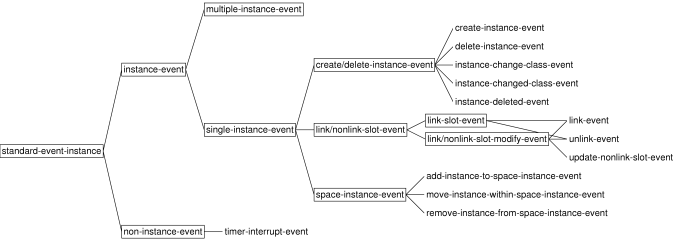
\includegraphics[scale=0.85]{gbbopen-events}
\end{center}
\W\end{iftex}

\noindent The event classes shown within rectangles are abstract classes
that cannot be signalled.

\W\xml{p}

Here are the defined event subclasses when both the
\code{:gbbopen-core} and \code{:agenda-shell} modules have been loaded:

\T\begin{ifhtml}
\xml{br}
\xml{img align="center" src="agenda-shell-events.png"}
\xml{br clear="both"}
\T\end{ifhtml}
\W\begin{iftex} 
\begin{center}
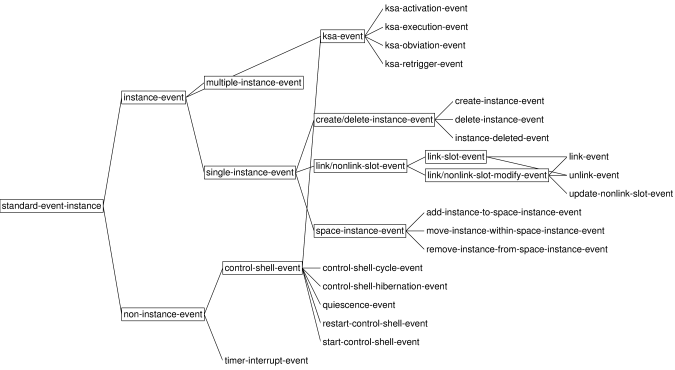
\includegraphics[scale=0.85]{agenda-shell-events}
\end{center}
\W\end{iftex}

\noindent The additional \code{control-shell-event} classes are
defined and signalled by the Agenda Shell.  Again classes shown within
rectangles are abstract classes that cannot be signalled.

\begin{alsos}{standard-event-class}
\also[print-instance-slots]
\also[standard-gbbopen-instance]
\also[standard-event-class]
\end{alsos}

\end{functiondoc}

%% ------------------------------------------------------------------------

\begin{functiondoc}{Class}{standard-space-class}{}
\index{class!standard-space-class@\textbf{standard-space-class}}%
  
\fnsyntax

\fnpackage \code{:gbbopen}

\fnmodule \code{:gbbopen-core}

\fndescription 
\bfindexit{define-space-class}%
\bfindexit{standard-unit-class}%
The class \textbf{standard-space-class} is the default class of
\glref{space~classes} defined by \textbf{\entlinknoex{define-space-class}}.
It is a subclass of \textbf{\entlinknoex{standard-unit-class}}.

\begin{alsos}{standard-space-instance}
\also[standard-space-instance]
\also[standard-unit-class]
\end{alsos}

\end{functiondoc}

%% ------------------------------------------------------------------------

\begin{functiondoc}{Unit~Class}{standard-space-instance}{}
\index{class!standard-space-instance@\textbf{standard-space-instance}}%
\index{unit class!standard-space-instance@\textbf{standard-space-instance}}%

\fnsyntax

\fnpackage \code{:gbbopen}

\fnmodule \code{:gbbopen-core}

\fndescription \bfindexit{make-space-instance}%
\bfindexit{standard-unit-instance}%
The class \textbf{standard-space-instance} is the default \glref{class} of
\glref{instances} created by \textbf{\entlinknoex{make-space-instance}}.  A
\glref{space~instance} is also a \glref{unit~instance}, so
\textbf{standard-space-instance} is a subclass of
\textbf{\entlinknoex{standard-unit-instance}}.

\begin{alsos}{standard-unit-instance}
\also[print-instance-slots]
\also[standard-space-class]
\also[standard-unit-instance]
\end{alsos}

\end{functiondoc}

%% ------------------------------------------------------------------------

\begin{functiondoc}{Class}{standard-unit-class}{}
\index{class!standard-unit-class@\textbf{standard-unit-class}}%

\fnsyntax

\fnpackage \code{:gbbopen}

\fnmodule \code{:gbbopen-core}

\fndescription 
\bfindexit{define-unit-class}%
The class \textbf{standard-unit-class} is the default class of classes defined
by \textbf{\entlinknoex{define-unit-class}}.  It is a subclass of
\code{standard-class}.

\begin{alsos}{standard-unit-instance}
\also[define-unit-class]
\also[standard-unit-instance]
\also[standard-space-class]
\end{alsos}

\end{functiondoc}

%% ------------------------------------------------------------------------

\begin{functiondoc}{Unit~Class}{standard-unit-instance}{}
\index{class!standard-unit-instance@\textbf{standard-unit-instance}}%
\index{unit class!standard-unit-instance@\textbf{standard-unit-instance}}%
  
\fnsyntax

\fnpackage \code{:gbbopen}

\fnmodule \code{:gbbopen-core}

\fndescription 
\bfindexit{standard-unit-class}%
\bfindexit{standard-space-instance}%
The class \textbf{standard-unit-instance} is an \glref{instance} of
\textbf{\entlinknoex{standard-unit-class}} and is a superclass of every
\glref{unit~class} that is an \glref{instance} of
\textbf{\entlinknoex{standard-unit-class}} except itself.  It is a subclass
of \textbf{\glref{standard-gbbopen-instance}}.

A \glref{space~instance} is also a \glref{unit~instance}, so
\textbf{\entlinknoex{standard-space-instance}} is a superclass of
\textbf{standard-unit-instance}.

\begin{alsos}{standard-space-instance}
\also[print-instance-slots]
\also[standard-gbbopen-instance]
\also[standard-space-instance]
\also[standard-unit-class]
\end{alsos}

\end{functiondoc}

%% ------------------------------------------------------------------------

\begin{functiondoc}{Function}{suspend-event-printing}%
{[\var{event-class-specifier\/} 
[\var{unit-class-or-instance-specifier\/}]] \\
\code{\&key} \var{slot-names paths\/}}
\index{event printing!suspending}%

%% Although the [] syntax is normally used for macros to denote optional
%% arguments, here we use them rather than &optional because of the 
%% keyword-driven argument parsing used in this function.

\fnsyntax

\fnpurpose Suspend the printing of printing-enabled events for one or more
\glref{event~classes}. 

\fnpackage \code{:gbbopen}

\fnmodule \code{:gbbopen-core}

\fnargs
\begin{args}{unit-class-or-instance-specifier}
\arg[event-class-specifier] An \glref{extended~event-class~specification} 
(see below; default is \code{t})
\arg[unit-class-or-instance-specifier] An 
\glref{extended~unit-class~or~instance~specification} 
(see below; default is \code{t})
\arg[slot-names\/ \textrm{or} slot-name \T\hfil] A slot-name or list of slot-names
(default is \code{t})
\arg[paths\/ \textrm{or} path \T\hfil] A \glref{space-instance~path} regular expression
(default is \code{(*)})
\end{args}

\fndsyntax
\eventclassspec
\subeventingspec
\syntaxsep
\unitclassinstancespec
\subclassingspec

\fndescription 
Suspending event printing is a convenient way of switching off event
printing without losing event-printing enabled/disabled settings.
Disabled event printing remains disabled if event printing is
resumed (by using \textbf{\entlinknoex{resume-event-printing}}).

The \var{paths\/} argument is either the symbol \code{t} (indicating
all \glref{space~instances}) or a list representing a regular
expression where the following reserved symbols are interpreted as
follows:
\spaceinstanceregexp

\begin{alsos}{describe-event-printing}
\also[describe-event-printing]
\also[disable-event-printing]
\also[enable-event-printing]
\also[resume-event-printing]
\end{alsos}

\fnexample
Suspend all event printing associated with \code{possible-hyp}
\glref{unit~instances}: 
\begin{example}
  (suspend-event-printing 't 'possible-hyp)
\end{example}

\fnnote
\instanceevfnsnyi

\end{functiondoc}

%% ------------------------------------------------------------------------

\begin{functiondoc}{Generic~Function}{unit-class-dimensions}%
  {\var{unit-classes-specifier\/}
    \returns{} \var{dimension-list\/}}
\index{dimensions!inquiring, of a unit class}%
\index{unit class!finding dimensions of}%

\fnsyntax

\fnpurpose Return the \glref{dimension} specifications for instances
of a \glref{unit~class}.

\fnmethods
\fnalternate{unit-class-dimensions}%
  {\code{(}\var{unit-classes-specifier\/} \code{cons)}
    \returns{} \var{dimension-list\/}}
\fnalternate{unit-class-dimensions}%
  {\code{(}\var{unit-class\/} \code{standard-unit-class)}
    \returns{} \var{dimension-list\/}}

\fnpackage \code{:gbbopen}

\fnmodule \code{:gbbopen-core}

\fnargs
\begin{args}{unit-classes-specifier}
  \arg[unit-classes-specifier] An \glref{extended~unit-classes~specification}
  or a list of \glref{extended~unit-classes~specifications}
\end{args}

\fnreturns A list of \glref{dimension~name}, \glref{dimension~type} pairs.

\begin{alsos}{space-instance-dimensions}
\also[define-unit-class]
\also[space-instance-dimensions]
\end{alsos}

\fnexample
Return the \glref{dimensions} defined for instances of
\glref{unit~class} \code{hyp}: 
\begin{example}
> (unit-class-dimensions 'hyp)
((x :ordered) (y :ordered) (belief :ordered) (classification :enumerated))
\end{example}

\end{functiondoc}

%% ------------------------------------------------------------------------

\begin{functiondoc}{Macro}{unlinkf}%
  {\var{\glref{link-slot-place} unit-instance-or-instances\/}
    \returns{} \var{unit-instance-or-instances\/}} 
\index{unit instance!removing links between}%
\index{link!removing}%

\fnsyntax

\fnpurpose Remove a \glref{link} between a \glref{unit~instance} and one
or more \glref{unit~instances}.

\fnpackage \code{:gbbopen}

\fnmodule \code{:gbbopen-core}

\fnargs
\begin{args}{unit-instance-or-instances}
\arg[\glref{link-slot-place}] A form which is suitable for use as a
\glref{generalized~reference} to a \glref{link~slot}
\arg[unit-instance-or-instances] A \glref{unit~instance} or a
list of \glref{unit~instances}
\end{args}

\fnreturns The supplied \var{unit-instance-or-instances}.

\fnevents
\index{events!generated by!unlinkf@\textbf{unlinkf}}%
\index{events!unlink-event@\code{unlink-event}|itidx}%
\codeindexit{unlink-event}%
An \code{unlink-event} is signaled for:
\begin{tightitemize}
\item all pointers that are removed from the specified
  \glref{link-slot-place}
\item each inverse pointer of the \glref{link} that is removed from
  another \glref{unit~instance}
\end{tightitemize}

\begin{alsos}{unlinkf-all}
\also[linkf]
\also[link-setf]
\also[unlinkf-all]
\end{alsos}

\fnexample Remove \code{support-hyp} from the \code{supporting-hyps}
\glref{link~slot} of the \code{hyp} \glref{unit~instance}
\code{unit-instance}:
\begin{example}
> (unlinkf (supporting-hyps-of unit-instance) support-hyp)
#<hyp 231 (1488 7405) .63>
\end{example}

\end{functiondoc}

%% ------------------------------------------------------------------------

\begin{functiondoc}{Macro}{unlinkf-all}{\var{\glref{link-slot-place}\/}}
\index{unit instance!removing links between}%
\index{link!removing}%

\fnsyntax

\fnpurpose Remove all the \glref{links} in the specified
\glref{link~slot}.

\fnpackage \code{:gbbopen}

\fnmodule \code{:gbbopen-core}

\fnargs
\begin{args}{link-slot-place}
\arg[\glref{link-slot-place}] A form which is suitable for use as a
\glref{generalized~reference} to a \glref{link~slot}
\end{args}

\fnevents
\index{events!generated by!unlinkf-all@\textbf{unlinkf-all}}%
\index{events!unlink-event@\code{unlink-event}|itidx}%
\codeindexit{unlink-event}%
An \code{unlink-event} is signaled for:
\begin{tightitemize}
\item all pointers that are removed from the specified
  \glref{link-slot-place}
\item each inverse pointer of the \glref{link} that is removed from
  another \glref{unit~instance}
\end{tightitemize}

\begin{alsos}{link-setf}
\also[linkf]
\also[link-setf]
\also[unlinkf]
\end{alsos}

\fnexample
Remove all supporting hypothesis \glref{links} from the
\code{supporting-hyps} \glref{link~slot} of the \code{hyp}
\glref{unit~instance} \code{unit-instance}:  
\begin{example}
  (unlinkf-all (supporting-hyps-of unit-instance))
\end{example}

\end{functiondoc}

%% ------------------------------------------------------------------------

\begin{functiondoc}{Macro}{with-changing-dimension-values}%
  {\code{(}\var{unit-instance\/} 
         \[\var{dimension-name\/}\superstar{}\]\code{)}
    \var{declaration\/}\superstar{}
    \var{form\/}\superstar{}
    \returns{} \var{result\/}\superstar}
\index{unit instance!storage repositioning}%
  
\fnsyntax

\fnpurpose Inform GBBopen that the dimensional values of a
\glref{unit~instance} will potentially be changed by the evaluation of
\var{forms}.

\fnpackage \code{:gbbopen}

\fnmodule \code{:gbbopen-core}

\fnargs
\begin{args}{dimension-name}
\arg[unit-instance] A \glref{unit~instance}
\arg[dimension-name] A symbol specifying a \glref{dimension} of
  \var{unit-instance} 
\arg[declaration] A declare expression
\arg[forms] An implicit \textbf{progn} of \glref{forms} to be evaluated
\end{args}

\fnreturns The values returned by evaluating the last \var{form}.

\fndescription The indexing for \var{unit-instance\/} is updated following the
evaluation of the last \var{form}.  Any retrieval operations performed during
the evaluation of \var{forms\/} may operate with indexes as they existed
before evaluation of the first \var{form}; therefore, retrievals should not be
included within the scope of \textbf{with-changing-dimension-values}.
Retrievals performed by separate threads also should be synchronized with
\textbf{with-changing-dimension-values}.

If \var{dimension-names\/} are specified, only the indexes for those
\glref{dimensions} of \var{unit-instance\/} will be updated. If no
\var{dimension-names\/} are specified, the values of any or all
\glref{dimensions} of \var{unit-instance\/} are assumed to have been
potentially changed by \var{forms}.

\fnexamples Notify GBBopen that the \code{x}, \code{y}, and \code{belief}
dimension values of \code{hyp} might be changed:
\begin{example}
> (with-changing-dimension-values (hyp x y belief)
    (setf (location-of hyp) '(30 40))
    (setf (belief-of hyp) 0.78))
\end{example}

Notify GBBopen that some dimension values of \code{hyp} might be changed:
\begin{example}
> (with-changing-dimension-values (hyp)
    (setf (location-of hyp) '(36 52))
    (incf (belief-of hyp) 0.05))
\end{example}

\end{functiondoc}

%% ------------------------------------------------------------------------

\begin{functiondoc}{Macro}{with-events-disabled}%
  {\code{(}\var{option\/}\superstar{}\code{)}
    \var{declaration\/}\superstar{}
    \var{form\/}\superstar{}
    \returns{} \var{result\/}\superstar}
\index{disabling!event signaling}%
\index{events!disabling signaling of}%
  
\fnsyntax

\fnpurpose Disable event signaling during evaluation of \var{forms}.

\fnpackage \code{:gbbopen}

\fnmodule \code{:gbbopen-core}

\fnargs
\begin{args}{options}
\arg[option] No options are currently supported
\arg[declaration] A declare expression
\arg[forms] An implicit \textbf{progn} of \glref{forms} to be evaluated
\end{args}

\fnreturns The values returned by evaluating the last \var{form}.

\begin{alsos}{with-events-enabled}
\also[signal-event]
\also[with-events-enabled]
\end{alsos}

\fnexample
\bfindexit{make-instance}%
Create a \code{hyp} without signaling any events:
\begin{example}
> (with-events-disabled ()
     (\entlink{make-instance} 'hyp 
        :location (list x y)
        :identity '(:car :truck :bus :motorcycle :duck-boat)
        :belief .85
        :supporting-hyps supporting-hyps))
#<hyp 119 (1835 4791) .85>
\end{example}

\end{functiondoc}

%% ------------------------------------------------------------------------

\begin{functiondoc}{Macro}{with-events-enabled}%
  {\code{(}\var{option\/}\superstar{}\code{)}
    \var{declaration\/}\superstar{}
    \var{form\/}\superstar{}
    \returns{} \var{result\/}\superstar}
\index{enabling event signaling}%
\index{events!enabling signaling of}%
  
\fnsyntax

\fnpurpose Restore event signaling during evaluation of \var{forms}.

\fnpackage \code{:gbbopen}

\fnmodule \code{:gbbopen-core}

\fnargs
\begin{args}{options}
\arg[option] No options are currently supported
\arg[declaration] A declare expression
\arg[forms] An implicit \textbf{progn} of \glref{forms} to be evaluated
\end{args}

\fnreturns The values returned by evaluating the last \var{form}.

\begin{alsos}{with-events-disabled}
\also[signal-event]
\also[with-events-disabled]
\end{alsos}

\fnexample
\bfindexit{make-instance}%
Create a \code{hyp} without signaling any events, then add
supporting-hypothesis links with events enabled:
\begin{example}
> (\entlink{with-events-disabled}
     (let ((hyp (\entlink{make-instance} 'hyp 
                    :location (list x y)
                    :identity '(:car :truck :bus :motorcycle :duck-boat)
                    :belief .85)))
        (with-events-enabled ()
           (linkf (supporting-hyps-of hyp) supporting-hyps))
        hyp))
#<hyp 119 (1835 4791) .85>
\end{example}

\end{functiondoc}

%% ------------------------------------------------------------------------

\begin{functiondoc}{Macro}{with-find-stats}%
  {\code{(}\code{\&key} \var{initialize report\/}\code{)}
    \var{declaration\/}\superstar{}
    \var{form\/}\superstar{} 
    \returns{} \var{result\/}\superstar}
\index{enabling retrieval statistics gathering}%
\index{displaying retrieval statistics}%
\index{find statistics!collecting and displaying}%
\index{retrieval!statistics, collecting and displaying}%
  
\fnsyntax

\fnpurpose 
\bfindexit{find-instances}%
\bfindexit{map-instances-on-space-instances}%
Record and optionally display retrieval statistics for 
\textbf{\entlinknoex{find-instances}} and
\textbf{\entlinknoex{map-instances-on-space-instances}}.

\fnpackage \code{:gbbopen}

\fnmodule \code{:gbbopen-core}

\fnargs
\begin{args}{initialize}
\arg[initialize] A \glref{generalized~boolean}(default is \code{t})
\arg[report] A \glref{generalized~boolean}(default is \code{t})
\arg[declaration] A declare expression
\arg[forms] An implicit \textbf{progn} of \glref{forms} to be evaluated
\end{args}

\fnreturns The values returned by evaluating the last \var{form}.

\begin{alsos}{map-instances-on-space-instances}
\also[find-instances]
\also[map-instances-on-space-instances]
\also[report-find-stats]
\also[without-find-stats]
\end{alsos}

\fnexample
\bfindexit{find-instance-by-name}%
Collect and display the retrieval statistics associated with
running an application \glref{function} \code{scanner}:
\begin{example}
> (with-find-stats ()
     (scanner (\entlink{find-instance-by-name} 471 'hyp)))
;; Find/Map Statistics:
;;        20 find/map operations (0 using marking, 20 using hashing)
;;       100 buckets scanned
;;      9240 instances touched
;;      9240 instances considered
;;       521 instances accepted
;;      0.16 seconds (0.80 msec/operation)
(#<hyp 119 (1835 4791) .85>
 #<hyp 233 (1835 4791) .89>)
\end{example}

\end{functiondoc}

%% ------------------------------------------------------------------------

\begin{functiondoc}{Macro}{without-find-stats}%
  {\var{declaration\/}\superstar{}
    \var{form\/}\superstar{}
    \returns{} \var{result\/}\superstar} 
\index{disabling!retrieval statistics gathering}%
\index{find statistics!disabling collection of}%
\index{retrieval!statistics, disabling collection of}%
  
\fnsyntax

\fnpurpose 
\bfindexit{find-instances}%
\bfindexit{map-instances-on-space-instances}%
Disable the collecting of retrieval statistics while executing \var{forms}.

\fnpackage \code{:gbbopen}

\fnmodule \code{:gbbopen-core}

\fnargs
\begin{args}{forms}
\arg[declaration] A declare expression
\arg[forms] An implicit \textbf{progn} of \glref{forms} to be evaluated
\end{args}

\fnreturns The values returned by evaluating the last \var{form}.

\begin{alsos}{with-find-stats}
\also[with-find-stats]
\end{alsos}

\fnexample
\bfindexit{find-instance-by-name}%
\bfindexit{with-find-stats}%
Collect and display the retrieval statistics associated with
running an application \glref{function} \code{scanner}:
\begin{example}
> (\entlink{with-find-stats} ()
     (scanner (\entlink{find-instance-by-name} 471 'hyp))
     (without-find-stats
        (scanner (\entlink{find-instance-by-name} 632 'hyp))))
;; Find/Map Statistics:
;;        20 find/map operations (0 using marking, 20 using hashing)
;;       100 buckets scanned
;;      9240 instances touched
;;      9240 instances considered
;;       521 instances accepted
;;      0.16 seconds (0.80 msec/operation)
(#<hyp 319 (1835 8419) .91>
 #<hyp 331 (1835 8419) .88>)
\end{example}

\end{functiondoc}

%% ========================================================================
%%  Agenda Control Shell

\T\markright{}%
\T\pagestyle{plain}
\T\cleardoublepage
\W\xname{ref-agenda-shell-entities}
\T\pagestyle{fancy}
\T\thispagestyle{fancybottom}
\T\global\def\fnlastname{ }%
\T\renewcommand{\headrulewidth}{0pt}
\section{Agenda Control Shell}

\index{module!:agenda-shell@\code{:agenda-shell}}%
\index{:agenda-shell@\code{:agenda-shell} module}%
The Agenda Shell module, \code{:agenda-shell}, provides a responsive,
agenda-based control shell.

\W\entities
\T\clearpage
\T\renewcommand{\headrulewidth}{0.01pt}

%% ------------------------------------------------------------------------

\begin{functiondoc}{Function}{abort-ks-execution}{\noargs}
\index{knowledge source execution!aborting}%

\fnsyntax

\fnpurpose Abort the currently executing KSA.

\fnpackage \code{:agenda-shell}

\fnmodule \code{:agenda-shell}

\begin{alsos}{exit-control-shell}
\also[exit-control-shell]
\end{alsos}

\fnexample
Abort the currently executing KSA::
\begin{example}
  (abort-ks-execution)
\end{example}

\end{functiondoc}

%% ------------------------------------------------------------------------

\begin{functiondoc}{Generic~Reader}{activation-cycle-of}{\var{ksa\/} 
    \returns{} \var{cycle-number\/}}
\index{activation cycle, of a KSA}%
\index{KSA!activation cycle of}%

\fnsyntax

\fnpurpose Returns the cycle number when a \glref{KSA} was activated

\fnmethods
\fnalternate{activation-cycle-of}{\code{(}\var{ksa\/} \code{ksa)}
  \returns{} \var{cycle-number\/}}

\fnpackage \code{:agenda-shell}

\fnmodule \code{:agenda-shell}

\fnargs
\begin{args}{ksa}
\arg[ksa] A \glref{KSA}
\end{args}

\fnreturns The activation cycle number of \var{ksa}
  
\fndescription 
This \glref{generic~function} accesses the value stored in the 
\code{activation-cycle} nonlink slot of \var{ksa}.  This value is
maintained by the Agenda Shell and should not be changed.

\begin{alsos}{ksa}
\also[ksa]
\end{alsos}

\fnexample
Return the activation cycle of \code{ksa}:
\begin{example}
> (activation-cycle-of ksa)
1192
\end{example}

\end{functiondoc}

%% ------------------------------------------------------------------------

\begin{functiondoc}{Generic~Function}{collect-trigger-instances}{\var{source\/}
    \returns{} \var{trigger-instances\/}} 
\index{trigger unit instance, of a KSA or event}%
\index{KSA!collecting trigger unit instances of}%
\index{event!collecting trigger unit instances of}%

\fnsyntax

\fnpurpose Return the trigger \glref{unit~instances} of a \glref{KSA},
\glref{event}, or a list of \glref{KSAs} or \glref{events}

\fnmethods
\fnalternate{collect-trigger-instances}%
  {\code{(}\var{cons\/} \code{cons)}
  \returns{} \var{trigger-instances}}
\fnalternate{collect-trigger-instances}%
  {\code{(}\var{event\/} \code{single-instance-event)}
  \returns{} \var{trigger-instances}}
\fnalternate{collect-trigger-instances}%
  {\code{(}\var{ksa\/} \code{ksa)}
  \returns{} \var{trigger-instances}}
\fnalternate{collect-trigger-instances}%
  {\code{(}\var{event\/} \code{multiple-instance-event)}
    \returns{} \var{trigger-instances}}
\fnalternate{collect-trigger-instances}%
  {\code{(}\var{event\/} \code{non-instance-event)}
  \returns{} \nil}

\fnpackage \code{:agenda-shell}

\fnmodule \code{:agenda-shell}

\fnargs
\begin{args}{source}
\arg[source] A \glref{KSA}, \glref{event},
or a list of \glref{KSAs} or \glref{events}
\end{args}

\fnreturns The list of trigger \glref{unit~instances}
  
\begin{alsos}{sole-trigger-instance-of}
\also[sole-trigger-instance-of]
\end{alsos}

\fnexample
Return the trigger \glref{unit~instances} of a KSA:
\begin{example}
> (collect-trigger-instances ksa)
(#<hyp 119 (1835 4791) .85>
 #<hyp 233 (1835 4791) .89>)
\end{example}

\end{functiondoc}

%% ------------------------------------------------------------------------

\begin{functiondoc}{Function}{control-shell-running-p}{\noargs{}
    \returns{} \var{boolean\/}}

\fnsyntax

\fnpurpose Return a value indicating whether a control shell is running.

\fnpackage \code{:agenda-shell}

\fnmodule \code{:agenda-shell}

\fnreturns True if the control shell is running; \nil{} otherwise.

\begin{alsos}{restart-control-shell}
\also[start-control-shell]
\also[restart-control-shell]
\end{alsos}

\fnexample
See if the control shell is running:
\begin{example}
> (control-shell-running-p)
nil
\end{example}

\end{functiondoc}

%% ------------------------------------------------------------------------

\begin{functiondoc}{Macro}{define-ks}{\var{ks-name\/} \code{\&key}
  \var{activation-predicate enabled execution-function 
       ks-class ksa-class
       obviation-events obviation-predicate 
       precondition-function rating
       retrigger-events retrigger-function 
       revalidation-predicate trigger-events\/} 
   \returns{} \var{ks\/}}
\index{knowledge source!defining/redefining}%
\index{defining!a knowledge source}%
\index{redefining!a knowledge source}%

\fnsyntax

\fnpurpose Define or redefine a \glref{knowledge~source} (KS).

\fnpackage \code{:agenda-shell}

\fnmodule \code{:agenda-shell}

\fnargs
\begin{args}{revalidation-predicate}
\arg[ks-name] A symbol naming the \glref{KS} (not evaluated)
\arg[activation-predicate] A \glref{function} of two arguments (the
\glref{KS} \glref{unit~instance} and the \glref{event} object) that returns a
\glref{generalized~boolean} or \nil{}
(default is \nil) 
\arg[enabled] A \glref{generalized~boolean} (default is \code{t})
\arg[execution-function]  A \glref{function} of one argument (the
\glref{KSA} \glref{unit~instance}) or \nil{} (default is \nil)
\arg[ks-class] A class or a symbol specifying a class (not evaluated)
\arg[ksa-class] A class or a symbol specifying a class (not evaluated)
\arg[obviation-events] An \var{event-specification\/} (see below, 
not evaluated)
\arg[obviation-predicate]  A \glref{function} of two arguments (the
\glref{KSA} \glref{unit~instance} and the \glref{event} object) that returns a
\glref{generalized~boolean} or \nil{}
(default is \nil) 
\arg[precondition-function] A \glref{function} of two arguments (the
\glref{KS} \glref{unit~instance} and the \glref{event} object) or \nil{}
(default is \nil) 
\arg[rating] A \glref{rating} (default is \code{1})
\arg[retrigger-events] An \var{event-specification\/} (see below, 
not evaluated)
\arg[retrigger-function] A \glref{function} of two arguments (the
\glref{KSA} \glref{unit~instance} and the \glref{event} object) or \nil{}
(default is \nil) 
\arg[revalidation-predicate] A \glref{function} of one argument (the
\glref{KSA} \glref{unit~instance}) that returns a
\glref{generalized~boolean} or \nil{} (default is \nil)
\arg[trigger-events] An \var{event-specification\/} (see below, not evaluated)

\end{args}

\fnreturns The \glref{unit~instance} representing the \glref{KS}

\fndsyntax
\begin{tabular}{@{~}l@{~}l}
\mbox{\var{event-specification\/} ::=}
  & \code{(}\var{event-signature\/}\superstar\code{)} \\
\end{tabular}
\T\\
\begin{tabular}{@{~}l@{~}l}
\mbox{\var{event-signature\/} ::=}
  & \code{(}\var{event-class-specifier\/} \\
  & ~ ~  [\var{unit-class-or-instance-specifier\/} \\
  & ~ ~ ~ ~ [\{\code{:slot-name} \var{slot-name\/}\} \vbar{} 
             \{\code{:slot-names} \var{slot-names\/}\} \vbar{} \\
  & ~ ~ ~ ~ ~ \{\code{:path} \var{path\/}\} \vbar{} 
              \{\code{:paths} \var{paths\/}\}]]\code{)} \\
\end{tabular}
\syntaxsep
\eventclassspec
\subeventingspec
\syntaxsep
\unitclassinstancespec
\subclassingspec

\fndescription
A \glref{KS} definition creates a \glref{unit~instance} of class
\var{ks-class\/} which specifies how \glref{activations} of the \glref{KS} are
created and executed.  The lifetime of each \glref{KS~activation} involves the
following sequence:

\begin{tightitemize}
\item When an \glref{event} matching one of the event specifications in
  \var{trigger-events\/} occurs and the \glref{KS} is enabled:
\begin{tightitemize}
\item the \var{activation-predicate\/}, if specified, is called and must
  return true for potential \glref{activation} to continue
\item the \var{precondition-function\/}, if specified, is called and must
  return an integer rating for potential \glref{activation} to continue
\end{tightitemize}
\item The \glref{KS} is activated (a \glref{unit~instance} of class
  \var{ksa-class\/} is created) and given the rating returned by the
  \var{precondition-function\/} or the constant \var{rating} value defined for
  the \glref{KS} if no \var{precondition-function\/} was specified.  The
  current control-shell cycle number is stored in the \code{activation-cycle}
  slot of the \glref{KSA} \glref{unit~instance}.
\item The \glref{KSA} is placed on the queue of
  \glref{pending~KSAs}.
\item If an \glref{event} matching one of the event specifications in
  \var{obviation-events\/} occurs, the \var{obviation-predicate\/}, if
  specified, is called.  If it returns true, the \glref{pending~KSA} is
  removed from the \glref{pending~KSAs} queue, the current
  control-shell cycle number is stored in the \code{obviation-cycle} slot of
  the \glref{KSA}, and the \glref{KSA} is placed on the queue of
  \glref{obviated~KSAs}.
\item If an \glref{event} matching one of the event specifications in
  \var{retrigger-events\/} occurs, the \var{retrigger-function\/}, if
  specified, is called.  A \var{retrigger-function\/} is often used to change
  the triggering context of the \glref{KSA} or its rating.
\indexit{minimum-ksa-execution-rating}%
\item When the \glref{pending~KSA} is selected for execution (typically
  because has the highest rating above the \var{minimum-ksa-execution-rating\/}
  currently in effect for the control shell), the
  \var{revalidation-predicate\/}, if specified, is called. If the
  \var{revalidation-predicate\/} returns \nil, the \glref{pending~KSA} is
  removed from the \glref{pending~KSAs} queue, the current
  control-shell cycle number is stored in the \code{obviation-cycle} slot of
  the \glref{KSA}, and the \glref{KSA}is placed on the queue of
  \glref{obviated~KSAs}.
\item The \glref{pending~KSA} is removed from the
  \glref{pending~KSAs} queue, the current control-shell cycle number
  is stored in the \code{execution-cycle} slot of the \glref{KSA}
  \glref{unit~instance}, and the \var{execution-function\/} is called.
\item The executed \glref{KSA} is placed on the queue of
  \glref{executed~KSAs}.
\end{tightitemize}

\fndspar{KS functions and predicates}

\codeindexqual{:stop}{value returned by a \glref{KS-execution} function}%
\index{agenda shell!exiting}%
\index{control shell!exiting}%
\index{exiting, agenda shell}%
\index{stopping, agenda shell}%
\index{KS!execution function}%
\index{execution function, of a KS}%
The Agenda Shell provides a rich set of \glref{KS} functions and predicates to
manage the progression of \glref{KSAs} from initial triggering and activation
through \glref{obviation} or execution.  A typicial \glref{KS} will only
require a subset of these functions and predicates.

An \var{activation-predicate\/} is a \glref{function} that is called with two
arguments, the \glref{unit~instance} representing the \glref{KS} and the
object representing the triggering event.  The \var{activation-predicate\/}
should return a \glref{generalized~boolean} that indicates whether the
\glref{KS} should continue to be considered for activation in response to the
event.  Typically, an \var{activation-predicate\/} is specified for a
\glref{KS} that does not require a \var{precondition-function\/} rating
computation, but that does require an activate/don't-activate decision.

A \var{precondition-function\/} is a \glref{function} that is called with two
arguments, the \glref{unit~instance} representing the \glref{KS} and the
object representing the triggering event.  The \var{precondition-function\/}
should return one of the following sets of values:
\begin{tightitemize}
\item \nil{} indicating the \glref{KS} is not to be activated in response to
  the event
\item \code{:stop} (and, optionally, additional values to be returned by the
  control shell) indicating that the control shell is to exit immediately
\item An integer execution \glref{rating} for the \glref{KSA} (and,
  optionally, initialization arguments to be used when creating the
  \glref{KSA} \glref{unit~instance})
\end{tightitemize}

An \var{execution-function\/} is a \glref{function} that implements the
\glref{KS}.  When an activation of the \glref{KS} is executed, this
\glref{function} is called with one argument, the \glref{unit~instance}
representing the \glref{KSA}. If the execution \glref{function} returns the value
\code{:stop} (and, optionally, a additional values to be returned by the
control shell), the control shell will exit immediately.

An \var{obviation-predicate\/} is a \glref{function} that is called with two
arguments, the \glref{unit~instance} representing the \glref{KSA} and the
object representing the \glref{obviation} event.  The \var{obviation-predicate\/}
should return a \glref{generalized~boolean} that indicates whether the
\glref{KSA} should be \glref{obviated}.

A \var{retrigger-function\/} is a \glref{function} that is called with
two arguments, the \glref{unit~instance} representing the \glref{KSA}
and the object representing the retrigger event.  The
\var{retrigger-function\/} can perform whatever activities are needed
in response to the event.  Typically this involves augmenting the
triggering context of the \glref{KSA} or changing its execution rating.

A \var{revalidation-predicate\/} is a \glref{function} that is called with one
argument, the \glref{unit~instance} representing the \glref{KSA}.  The
\var{revalidation-predicate\/} is called immediately before a \glref{KSA} is
executed and should return a \glref{generalized~boolean} that indicates
whether the \glref{KSA} should be executed (if true) or \glref{obviated} (if
false).

\begin{alsos}{standard-event-instance}
\also[define-ks-class]
\also[define-ksa-class]
\also[describe-ks]
\also[ensure-ks]
\also[ks]
\also[ks-enabled-p]
\also[standard-event-instance]
\also[undefine-ks]
\end{alsos}

\fnexamples
Define an initial \glref{KS} that is triggered when the control shell is started:
\begin{example}
  (define-ks inital
     :trigger-events ((start-control-shell-event)) 
     :execution-function #'initial-ks-function)
\end{example}

Define a \glref{KS} named \code{aggregate-hyps} that is triggered whenever a
\code{hyp} \glref{unit~instance} is created:
\begin{example}
  (define-ks aggregate-hyps
     :trigger-events ((create-instance-event hyp))
     :precondition-function #'aggregate-hyps-precondition-function
     :execution-function #'aggregate-hyps-ks-function)
\end{example}

\fnnote
\instancekstriggersnyi

\end{functiondoc}

%% ------------------------------------------------------------------------

\begin{functiondoc}{Macro}{define-ks-class}%
   {\var{ks-class-name\/} 
   \code{(}\{\var{superclass-name\/}\}\superstar\code{)}
   [\var{documentation\/}] \\
   \code{(}\{\var{slot-specifier\/}\}\superstar\code{)}
   \{\var{class-option\/}\}\superstar{} \returns{}
   \var{new-ks-class\/}}
\index{ks class!defining/redefining}%
\index{defining!a ks class}%
\index{redefining!a ks class}%

\fnsyntax

\fnpurpose Define or redefine a \glref{ks~class}.

\fnpackage \code{:agenda-shell}

\fnmodule \code{:agenda-shell}

\fnargs
\begin{args}{ks-class-name}
\arg[ks-class-name] A non-\nil, non-keyword symbol that names the
\glref{ks~class} 
\arg[superclass-name] A non-\nil, non-keyword symbol that specifies a
direct superclass of the \glref{ks~class} \var{ks-class-name\/}  
\arg[documentation] A documentation string
\arg[slot-specifiers] See below
\arg[class-options] See below
\end{args}

\fnreturns The newly defined \glref{ks~class} object.

\fnerrors The specified \var{superclass-names\/} do not include at least
one \glref{ks~class} name.  This error is signaled on class finalization.

\fndsyntax
\begin{tabular}{@{~}l@{~}l}
\mbox{\var{slot-specifier\/} ::=}
 & \var{slot-name\/} \vbar \\
 & \code{(}\var{nonlink-slot-name\/}
   [[\var{nonlink-slot-option\/}]]\code{)} \vbar \\
 & \code{(}\var{link-slot-name\/} [[\var{link-slot-option\/}]]\code{)} \\
\end{tabular}
\T\\
\begin{tabular}{@{~}l@{~}l}
\mbox{\var{nonlink-slot-name\/} ::=} & \var{slot-name}\\
\end{tabular}
\T\\
\begin{tabular}{@{~}l@{~}l}
\mbox{\var{link-slot-name\/} ::=} & \var{slot-name}\\
\end{tabular}
\T\\
\begin{tabular}{@{~}l@{~}l}
\mbox{\var{link-slot-option\/} ::=}
 & \var{slot-option\/} \vbar \\
 & \{\code{:link} \var{inverse-link-slot-specifier\/}\} \vbar \\
 & \{\code{:singular} \var{boolean\/}\} \vbar \\
 & \{\code{:sort-function} \var{function\/}\} \vbar \\
 & \{\code{:sort-key} \var{function\/}\} \\
\end{tabular}
\T\\
\begin{tabular}{@{~}l@{~}l}
\mbox{\var{inverse-link-slot-specifier\/} ::=} & 
  \code{(}\var{unit-class-name link-slot-name\/} 
    [\code{:singular} \var{boolean\/}]\code{)} \vbar{} \\
  & \code{:reflexive} \\
\end{tabular}
\T\\
\begin{tabular}{@{~}l@{~}l}
\mbox{\var{nonlink-slot-option\/} ::=}
 & \var{slot-option\/} \vbar \\
 & \{\code{:reader} \var{reader-function-name\/}\}\superstar{} \vbar \\
 & \{\code{:writer} \var{writer-function-name\/}\}\superstar{} \\
\end{tabular}
\T\\
\begin{tabular}{@{~}l@{~}l}
\mbox{\var{slot-option\/} ::=}
 & \{\code{:accessor} \var{reader-function-name\/}\}\superstar{} \vbar \\
 & \{\code{:allocation} \var{allocation-type\/}\} \vbar \\
 & \{\code{:documentation} \var{string\/}\} \vbar \\
 & \{\code{:initarg} \var{initarg-name\/}\}\superstar{} \vbar \\
 & \{\code{:initform} \var{form\/}\} \vbar \\
 & \{\code{:type} \var{type-specifier\/}\} \\
\end{tabular}
\T\\
\begin{tabular}{@{~}l@{~}l}
\mbox{\var{class-option\/} ::=}
 & \code{(:abstract} \var{boolean\/}\code{)} \vbar \\
 & \code{(:default-initargs .} \var{initarg-list\/}\code{)} \vbar \\
 & \code{(:dimensional-values} 
   \var{dimensional-value-spec\/}\superstar\code{)} \vbar \\
 & \code{(:documentation} \var{string\/}\code{)} \vbar \\
 & \code{(:export-class-name} \var{boolean\/}\code{)} \vbar \\
 & \code{(:export-accessors} \var{boolean\/}\code{)} \vbar \\
 & \code{(:generate-accessors} \var{direct-slots-specifier\/}\code{)} \vbar \\
 & \code{(:generate-accessors-format} 
     \{\code{:prefix} \vbar{} \code{:suffix}\} \vbar \\
 & \code{(:generate-accessors-prefix} \{\var{string\/} \vbar{}
     \var{symbol\/}\}\var\code{)} \vbar \\
 & \code{(:generate-accessors-suffix} \{\var{string\/} \vbar{}
     \var{symbol\/}\}\var\code{)} \vbar \\
 & \code{(:generate-initargs} \var{direct-slots-specifier\/}\code{)} \vbar \\
 & \code{(:initial-space-instances}
     \var{initial-space-instance-specifier\/}\code{)} \vbar \\
 & \code{(:instance-name-comparision-test}
     \var{instance-name-comparision-test\/}\code{)} \vbar \\
 & \code{(:metaclass} \var{class-name\/}\code{)} \\
\end{tabular}
\T\\
\begin{tabular}{@{~}l@{~}l}
\mbox{\var{initial-space-instance-specifier\/} ::=}
  & \{\var{space-instance-path\/}\superplus{} \vbar{}
  \var{function\/}\} \\ 
\end{tabular}
\T\\
\dimensionalvaluesspec
\T\\
\begin{tabular}{@{~}l@{~}l}
\mbox{\var{direct-slots-specifier\/} ::=} & \nil{} \vbar{} \code{t} \vbar{}
  \var{included-slot-name\/}\superstar{} \vbar \\
  & \{\code{t :exclude} \var{excluded-slot-name\/}\superstar{}\} \\
\end{tabular}

\fnterms
\begin{args}{instance-name-comparison-test}
\arg[class-name] A non-\nil, non-keyword symbol that names a
\glref{class} 
\arg[initarg-list] An \glref{initialization~argument~list}
\arg[slot-name] A non-\nil, non-keyword symbol
\arg[instance-name-comparison-test] One of the four standardized hash table
test function names: \code{eq}, \code{eql}, \code{equal}, or \code{equalp}
(default for classes of metaclass \textbf{\entlinknoex{standard-unit-class}}
is \code{eql})
\end{args}

\fndescription A \var{dimension-value-place\/} with two
\var{slot-names\/} can be specified only for \code{:interval}
dimension-value types.

\bfindexit{ks}%
Each \var{superclass-name} argument specifies a direct superclass of the new
class. If the superclass list is empty, then the direct superclass defaults to the
single class \textbf{\entlink{ks}}.

\bfindexit{standard-unit-class}%
The \code{:metaclass} \var{class-name\/}, if specified, must be a subclass of
\textbf{\entlinknoex{standard-unit-class}}.  The default metaclass value is
also \textbf{\entlinknoex{standard-unit-class}}.

\fndspar{Inheritance of class options}

\index{inheritance!unit-class options}%
\index{dimensional values!inheritance}%
\index{initial space instances!inheritance}%
The set of \var{dimensional-values\/} for a \glref{unit~class} is the
union of the sets specified in the \var{dimensional-values\/} options
of the class and its superclasses.  When more than one dimensional
index is supplied for a given dimension, the one supplied by the most
specific class is used.

The effective \var{initial-space-instances\/} value for a
\glref{unit~class} is the value specified in the definition of the
most specific \glref{unit~class}. If no definitions specify an
\var{initial-space-instances\/} value, \nil{} is used.

The \var{instance-name-comparison-test\/} value is not inherited.  If
no value is specified in the \glref{unit-class} definition, the
default initializtion value associated with the metaclass is used.

\begin{alsos}{with-generate-accessors-format}
\also[define-ks]
\also[standard-unit-class]
\also[with-generate-accessors-format]
\end{alsos}

\fnexamples
Define a \glref{ks~class},
\code{ks-with-lock}, that has an additional \glref{slot}
containing a \glref{lock} that can be used to synchronize
operations on each defined \glref{KS} of that class.
\begin{example}
> (define-ks-class ks-with-lock ()
    ((lock :initform (\entlink{make-lock} :name "KS Lock"))))
#<standard-unit-class ks-with-lock>
\end{example}

Do the same, but with a mixin class:
\begin{example}
> (define-unit-class lock-mixin (ks my-mixin)
    ((lock :initform (\entlink{make-lock} :name "KS Lock"))))
#<standard-unit-class lock-mixin>
> (define-ks-class ks-with-lock (ks lock-mixin)
    ())
#<standard-unit-class ks-with-lock>
\end{example}

\end{functiondoc}

%% ------------------------------------------------------------------------

\begin{functiondoc}{Macro}{define-ksa-class}%
   {\var{ksa-class-name\/} 
   \code{(}\{\var{superclass-name\/}\}\superstar\code{)}
   [\var{documentation\/}] \\
   \code{(}\{\var{slot-specifier\/}\}\superstar\code{)}
   \{\var{class-option\/}\}\superstar{} \returns{}
   \var{new-ksa-class\/}}
\index{ksa class!defining/redefining}%
\index{defining!a ksa class}%
\index{redefining!a ksa class}%

\fnsyntax

\fnpurpose Define or redefine a \glref{ksa~class}.

\fnpackage \code{:agenda-shell}

\fnmodule \code{:agenda-shell}

\fnargs
\begin{args}{ksa-class-name}
\arg[ksa-class-name] A non-\nil, non-keyword symbol that names the
\glref{ksa~class} 
\arg[superclass-name] A non-\nil, non-keyword symbol that specifies a
direct superclass of the \glref{ksa~class} \var{ksa-class-name\/}  
\arg[documentation] A documentation string
\arg[slot-specifiers] See below
\arg[class-options] See below
\end{args}

\fnreturns The newly defined \glref{ksa~class} object.

\fnerrors The specified \var{superclass-names\/} do not include at least
one \glref{ksa~class} name.  This error is signaled on class finalization.

\fndsyntax
\begin{tabular}{@{~}l@{~}l}
\mbox{\var{slot-specifier\/} ::=}
 & \var{slot-name\/} \vbar \\
 & \code{(}\var{nonlink-slot-name\/}
   [[\var{nonlink-slot-option\/}]]\code{)} \vbar \\
 & \code{(}\var{link-slot-name\/} [[\var{link-slot-option\/}]]\code{)} \\
\end{tabular}
\T\\
\begin{tabular}{@{~}l@{~}l}
\mbox{\var{nonlink-slot-name\/} ::=} & \var{slot-name}\\
\end{tabular}
\T\\
\begin{tabular}{@{~}l@{~}l}
\mbox{\var{link-slot-name\/} ::=} & \var{slot-name}\\
\end{tabular}
\T\\
\begin{tabular}{@{~}l@{~}l}
\mbox{\var{link-slot-option\/} ::=}
 & \var{slot-option\/} \vbar \\
 & \{\code{:link} \var{inverse-link-slot-specifier\/}\} \vbar \\
 & \{\code{:singular} \var{boolean\/}\} \vbar \\
 & \{\code{:sort-function} \var{function\/}\} \vbar \\
 & \{\code{:sort-key} \var{function\/}\} \\
\end{tabular}
\T\\
\begin{tabular}{@{~}l@{~}l}
\mbox{\var{inverse-link-slot-specifier\/} ::=} & 
  \code{(}\var{unit-class-name link-slot-name\/} 
    [\code{:singular} \var{boolean\/}]\code{)} \vbar{} \\
  & \code{:reflexive} \\
\end{tabular}
\T\\
\begin{tabular}{@{~}l@{~}l}
\mbox{\var{nonlink-slot-option\/} ::=}
 & \var{slot-option\/} \vbar \\
 & \{\code{:reader} \var{reader-function-name\/}\}\superstar{} \vbar \\
 & \{\code{:writer} \var{writer-function-name\/}\}\superstar{} \\
\end{tabular}
\T\\
\begin{tabular}{@{~}l@{~}l}
\mbox{\var{slot-option\/} ::=}
 & \{\code{:accessor} \var{reader-function-name\/}\}\superstar{} \vbar \\
 & \{\code{:allocation} \var{allocation-type\/}\} \vbar \\
 & \{\code{:documentation} \var{string\/}\} \vbar \\
 & \{\code{:initarg} \var{initarg-name\/}\}\superstar{} \vbar \\
 & \{\code{:initform} \var{form\/}\} \vbar \\
 & \{\code{:type} \var{type-specifier\/}\} \\
\end{tabular}
\T\\
\begin{tabular}{@{~}l@{~}l}
\mbox{\var{class-option\/} ::=}
 & \code{(:abstract} \var{boolean\/}\code{)} \vbar \\
 & \code{(:default-initargs .} \var{initarg-list\/}\code{)} \vbar \\
 & \code{(:dimensional-values} 
   \var{dimensional-value-spec\/}\superstar\code{)} \vbar \\
 & \code{(:documentation} \var{string\/}\code{)} \vbar \\
 & \code{(:export-class-name} \var{boolean\/}\code{)} \vbar \\
 & \code{(:export-accessors} \var{boolean\/}\code{)} \vbar \\
 & \code{(:generate-accessors} \var{direct-slots-specifier\/}\code{)} \vbar \\
 & \code{(:generate-accessors-format} 
     \{\code{:prefix} \vbar{} \code{:suffix}\} \vbar \\
 & \code{(:generate-accessors-prefix} \{\var{string\/} \vbar{}
     \var{symbol\/}\}\var\code{)} \vbar \\
 & \code{(:generate-accessors-suffix} \{\var{string\/} \vbar{}
     \var{symbol\/}\}\var\code{)} \vbar \\
 & \code{(:generate-initargs} \var{direct-slots-specifier\/}\code{)} \vbar \\
 & \code{(:initial-space-instances}
     \var{initial-space-instance-specifier\/}\code{)} \vbar \\
 & \code{(:instance-name-comparision-test}
     \var{instance-name-comparision-test\/}\code{)} \vbar \\
 & \code{(:metaclass} \var{class-name\/}\code{)} \\
\end{tabular}
\T\\
\begin{tabular}{@{~}l@{~}l}
\mbox{\var{initial-space-instance-specifier\/} ::=}
  & \{\var{space-instance-path\/}\superplus{} \vbar{}
  \var{function\/}\} \\ 
\end{tabular}
\T\\
\dimensionalvaluesspec
\T\\
\begin{tabular}{@{~}l@{~}l}
\mbox{\var{direct-slots-specifier\/} ::=} & \nil{} \vbar{} \code{t} \vbar{}
  \var{included-slot-name\/}\superstar{} \vbar \\
  & \{\code{t :exclude} \var{excluded-slot-name\/}\superstar{}\} \\
\end{tabular}

\fnterms
\begin{args}{instance-name-comparison-test}
\arg[class-name] A non-\nil, non-keyword symbol that names a
\glref{class} 
\arg[initarg-list] An \glref{initialization~argument~list}
\arg[slot-name] A non-\nil, non-keyword symbol
\arg[instance-name-comparison-test] One of the four standardized hash table
test function names: \code{eq}, \code{eql}, \code{equal}, or \code{equalp}
(default for classes of metaclass \textbf{\entlinknoex{standard-unit-class}}
is \code{eql})
\end{args}

\fndescription A \var{dimension-value-place\/} with two
\var{slot-names\/} can be specified only for \code{:interval}
dimension-value types.

\bfindexit{ksa}%
Each \var{superclass-name} argument specifies a direct superclass of the new
class. If the superclass list is empty, then the direct superclass defaults to the
single class \textbf{\entlink{ksa}}.

\bfindexit{standard-unit-class}%
The \code{:metaclass} \var{class-name\/}, if specified, must be a subclass of
\textbf{\entlinknoex{standard-ksa-class}}.  The default metaclass value is
also \textbf{\entlinknoex{standard-ksa-class}}.

\fndspar{Inheritance of class options}

\index{inheritance!unit-class options}%
\index{dimensional values!inheritance}%
\index{initial space instances!inheritance}%
The set of \var{dimensional-values\/} for a \glref{unit~class} is the
union of the sets specified in the \var{dimensional-values\/} options
of the class and its superclasses.  When more than one dimensional
index is supplied for a given dimension, the one supplied by the most
specific class is used.

The effective \var{initial-space-instances\/} value for a
\glref{unit~class} is the value specified in the definition of the
most specific \glref{unit~class}. If no definitions specify an
\var{initial-space-instances\/} value, \nil{} is used.

The \var{instance-name-comparison-test\/} value is not inherited.  If
no value is specified in the \glref{unit-class} definition, the
default initializtion value associated with the metaclass is used.

\begin{alsos}{with-generate-accessors-format}
\also[define-ks]
\also[standard-ksa-class]
\also[with-generate-accessors-format]
\end{alsos}

\fnexamples
Define a \glref{ksa~class},
\code{ksa-with-lock}, that has an additional \glref{slot}
containing a \glref{lock} that can be used to synchronize
operations on each \glref{KSA} of that class.
\begin{example}
> (define-ksa-class ksa-with-lock ()
    ((lock :initform (\entlink{make-lock} :name "KSA Lock"))))
#<standard-ksa-class ksa-with-lock>
\end{example}

Do the same, but with a mixin class:
\begin{example}
> (define-unit-class lock-mixin (ks my-mixin)
    ((lock :initform (\entlink{make-lock} :name "KS Lock"))))
#<standard-unit-class lock-mixin>
> (define-ksa-class ksa-with-lock (ksa lock-mixin)
    ())
#<standard-ksa-class ksa-with-lock>
\end{example}

\end{functiondoc}

%% ------------------------------------------------------------------------

\begin{functiondoc}{Generic~Function}{describe-ks}%
  {\var{ks-name\/}}
\index{KS!printing information about}%
\index{printing!information about!a KS}%

\fnsyntax

\fnpurpose
Print information about a \glref{knowledge~source} (KS).
 
\fnmethods
\fnalternate{describe-ks}{\code{(}\var{ks-name\/} \code{symbol)}}
\fnalternate{describe-ks}{\code{(}\var{ks\/} \code{ks)}}

\fnpackage \code{:agenda-shell}

\fnmodule \code{:agenda-shell}

\fnargs
\begin{args}{unit-class-name}
  \arg[unit-class-name] A \glref{unit-class} or a symbol specifying a
  \glref{unit~class}.
\end{args}

\fndescription
\bfindexit{*standard-output*}%
The description is printed to the {\bf *standard-output*} stream.

\begin{alsos}{define-ks}
\also[define-ks]
\also[ks]
\end{alsos}

\fnexample
\begin{example}
> (describe-ks 'start-control-shell-ks)

KS: start-control-shell-ks
  Trigger events:        ((start-control-shell-event))
  Precondition function: #<Function scse-precondition>
  Execution function:    #<Function scse-fn>
\end{example}

\end{functiondoc}

%% ------------------------------------------------------------------------

\begin{functiondoc}{Function}{ensure-ks}{\var{ks-name\/} \code{\&key}
  \var{activation-predicate enabled execution-function 
       ks-class ksa-class
       obviation-events obviation-predicate 
       precondition-function rating
       retrigger-events retrigger-function 
       revalidation-predicate trigger-events\/} 
   \returns{} \var{ks\/}}
\index{knowledge source!defining/redefining}%
\index{defining!a knowledge source}%
\index{redefining!a knowledge source}%

\fnsyntax

\fnpurpose Programatically define or redefine a \glref{knowledge~source} (KS).

\fnpackage \code{:agenda-shell}

\fnmodule \code{:agenda-shell}

\fnargs
\begin{args}{revalidation-predicate}
\arg[ks-name] A symbol naming the \glref{KS}
\arg[activation-predicate] A \glref{function} of two arguments (the
\glref{KS} \glref{unit~instance} and the \glref{event} object) that returns a
\glref{generalized~boolean} or \nil{}
(default is \nil) 
\arg[enabled] A \glref{generalized~boolean} (default is \code{t})
\arg[execution-function]  A \glref{function} of one argument (the
\glref{KSA} \glref{unit~instance}) or \nil{} (default is \nil)
\arg[ks-class] A class or a symbol specifying a class
\arg[ksa-class] A class or a symbol specifying a class
\arg[obviation-events] An \var{event-specification\/} (see below)
\arg[obviation-predicate]  A \glref{function} of two arguments (the
\glref{KSA} \glref{unit~instance} and the \glref{event} object) that returns a
\glref{generalized~boolean} or \nil{}
(default is \nil) 
\arg[precondition-function] A \glref{function} of two arguments (the
\glref{KS} \glref{unit~instance} and the \glref{event} object) or \nil{}
(default is \nil) 
\arg[rating] A \glref{rating} (default is \code{1})
\arg[retrigger-events] An \var{event-specification\/} (see below)
\arg[retrigger-function] A \glref{function} of two arguments (the
\glref{KSA} \glref{unit~instance} and the \glref{event} object) or \nil{}
(default is \nil) 
\arg[revalidation-predicate] A \glref{function} of one argument (the
\glref{KSA} \glref{unit~instance}) that returns a
\glref{generalized~boolean} or \nil{} (default is \nil)
\arg[trigger-events] An \var{event-specification\/} (see below)

\end{args}

\fnreturns The \glref{unit~instance} representing the \glref{KS}

\fndsyntax
\begin{tabular}{@{~}l@{~}l}
\mbox{\var{event-specification\/} ::=}
  & \code{(}\var{event-signature\/}\superstar\code{)} \\
\end{tabular}
\T\\
\begin{tabular}{@{~}l@{~}l}
\mbox{\var{event-signature\/} ::=}
  & \code{(}\var{event-class-specifier\/} \\
  & ~ ~  [\var{unit-class-or-instance-specifier\/} \\
  & ~ ~ ~ ~ [\{\code{:slot-name} \var{slot-name\/}\} \vbar{} 
             \{\code{:slot-names} \var{slot-names\/}\} \vbar{} \\
  & ~ ~ ~ ~ ~ \{\code{:path} \var{path\/}\} \vbar{} 
              \{\code{:paths} \var{paths\/}\}]]\code{)} \\
\end{tabular}
\syntaxsep
\eventclassspec
\subeventingspec
\syntaxsep
\unitclassinstancespec
\subclassingspec

\fndescription This function is called to define or redefine a \glref{KS}. It
is the functional equivalent of \textbf{\entlink{define-ks}} and is called by
the expansion of the \textbf{\entlink{define-ks}} macro.  (See the description
of \textbf{\entlink{define-ks}} for details of \glref{KS} definition and
redefinition.)

\begin{alsos}{define-ks}
\also[define-ks]
\also[ks]
\also[ks-enabled-p]
\also[undefine-ks]
\end{alsos}

\fnexample
Define an initial \glref{KS} that is triggered when the control shell is
started:
\begin{example}
  (ensure-ks 'inital
     :trigger-events '((start-control-shell-event)) 
     :execution-function #'initial-ks-function)
\end{example}

\end{functiondoc}

%% ------------------------------------------------------------------------

\begin{functiondoc}{Generic~Reader}{execution-cycle-of}{\var{ksa\/} 
    \returns{} \var{cycle-number\/}}
\index{execution cycle, of a KSA}%
\index{KSA!execution cycle of}%

\fnsyntax

\fnpurpose Returns the cycle number when a \glref{KSA} was executed

\fnmethods
\fnalternate{execution-cycle-of}{\code{(}\var{ksa\/} \code{ksa)}
  \returns{} \var{cycle-number\/}}

\fnpackage \code{:agenda-shell}

\fnmodule \code{:agenda-shell}

\fnargs
\begin{args}{ksa}
\arg[ksa] A \glref{KSA}
\end{args}

\fnreturns The execution cycle number of \var{ksa\/} or \nil, if \var{ksa\/} has
not been executed
  
\fndescription 
This \glref{generic~function} accesses the value stored in the 
\code{execution-cycle} nonlink slot of \var{ksa}. This value is
maintained by the Agenda Shell and should not be changed.

\begin{alsos}{ksa}
\also[ksa]
\end{alsos}

\fnexample
Return the execution cycle of \code{ksa}:
\begin{example}
> (execution-cycle-of ksa)
1237
\end{example}

\end{functiondoc}

%% ------------------------------------------------------------------------
 
\begin{functiondoc}{Function}{exit-control-shell}{\code{\&rest}
 \var{result-form\/}\superstar}
\index{agenda shell!exiting}%
\index{control shell!exiting}%
\index{exiting, agenda shell}%
\index{stoping, agenda shell}%

\fnsyntax

\fnpurpose Exit the Agenda Shell.

\fnpackage \code{:agenda-shell}

\fnmodule \code{:agenda-shell}

\fnargs
\begin{args}{result-form}
\arg[result-form] A \glref{form}
\end{args}

\fnerrors \textbf{Exit-control-shell} called outside the context of an
executing control shell.

\begin{alsos}{control-shell-running-p}
\also[abort-ks-execution]
\also[control-shell-running-p]
\also[restart-control-shell]
\also[start-control-shell]
\end{alsos}

\fnexample Exit the Agenda Shell, indicating that a solution, 
\code{solution}, was found:
\begin{example}
  (exit-control-shell ':solution-found solution)
\end{example}

\end{functiondoc}

%% ------------------------------------------------------------------------
 
\begin{functiondoc}{Function}{find-ks-by-name}{\var{ks-name\/} 
  \returns{} \var{ks\/}}
\index{KS!finding by name}%

\fnsyntax

\fnpurpose Return a ~\glref{KS} \glref{unit~instance} given its name

\fnpackage \code{:agenda-shell}

\fnmodule \code{:agenda-shell}

\fnargs
\begin{args}{ks-name}
\arg[ks-name] A symbol naming the \glref{KS}.
\end{args}

\fnreturns The \glref{KS} \glref{unit~instance} named \var{ks-name\/}
or \nil, if none has been defined.

\begin{alsos}{define-ks}
\also[define-ks]
\also[ks]
\end{alsos}

\fnexample Return the \glref{KS} named \code{start-control-shell-ks}:
\begin{example}
> (find-ks-by-name 'start-control-shell-ks)
#<ks start-control-shell-ks>
\end{example}

\end{functiondoc}

%% ------------------------------------------------------------------------

\begin{functiondoc}{Unit~Class}{ks}{}
\index{class!ks@\textbf{ks}}%
\index{unit class!ks@\textbf{ks}}%

\fnsyntax

\fnpackage \code{:agenda-shell}

\fnmodule \code{:agenda-shell}

\fndescription 
\bfindexit{define-ks}%
The class \textbf{ks} is the default \glref{class} of
\glref{instances} created by \textbf{\entlinknoex{define-ks}}.

\begin{alsos}{define-ks}
\also[define-ks]
\also[ksa]
\end{alsos}

\end{functiondoc}

%% ------------------------------------------------------------------------

\begin{functiondoc}{Unit~Class}{ksa}{}
\index{class!ksa@\textbf{ksa}}%
\index{unit class!ksa@\textbf{ksa}}%

\fnsyntax

\fnpackage \code{:agenda-shell}

\fnmodule \code{:agenda-shell}

\fndescription 
The class \textbf{ksa} is the default \glref{class} of
\glref{unit~instances} representing \glref{KS~activations}.

\begin{alsos}{ks}
\also[ks]
\end{alsos}

\end{functiondoc}

%% ------------------------------------------------------------------------

\begin{functiondoc}{Generic~Function}{ks-enabled-p}{\var{ks\/} 
    \returns{} \var{boolean\/}}
\index{KS!enabled}%

\fnsyntax

\fnpurpose Determine if the specified \glref{KS} is enabled for
execution

\fnsetf
\fnsetfsyntax{ks-enabled-p}{\var{ks\/}}{\var{boolean\/}}

\fnmethods
\fnalternate{ks-enabled-p}{\code{(}\var{ks\/} \code{ks)} 
  \returns{} \var{boolean\/}}
\fnalternate{(setf ks-enabled-p)}{\var{boolean\/} \code{(}\var{ks\/} \code{ks)}
  \returns{} \var{boolean\/}} 

\fnpackage \code{:agenda-shell}

\fnmodule \code{:agenda-shell}

\fnargs
\begin{args}{ks}
\arg[ks] A \glref{KS}
\arg[boolean] A \glref{generalized~boolean}
\end{args}

\fnreturns True if the \glref{KS} is enabled for execution; nil otherwise.
  
\fndescription 
This \glref{generic~function} accesses the value stored in the 
\code{enabled} nonlink slot of \var{ks\/}.

\begin{alsos}{undefine-ks}
\also[define-ks]
\also[ks]
\also[undefine-ks]
\end{alsos}

\fnexamples
See if \glref{KS} \var{ks} is enabled for execution:
\begin{example}
> (ks-enabled-p ks)
t
\end{example}

Now disable \glref{KS} \code{ks}:
\begin{example}
  (setf (ks-enabled-p ks) nil)
\end{example}

Check once again:
\begin{example}
> (ks-enabled-p ks)
nil
\end{example}

\end{functiondoc}

%% ------------------------------------------------------------------------

\begin{functiondoc}{Generic~Reader}{ks-of}{\var{ksa\/} 
    \returns{} \var{ks\/}}
\index{knowledge source!of a KSA}%
\index{KS!of a KSA}%
\index{KSA!KS of}%

\fnsyntax

\fnpurpose Returns the \glref{knowledge~source} (KS) \glref{unit~instance}
of a \glref{KSA}

\fnmethods
\fnalternate{ks-of}{\code{(}\var{ksa\/} \code{ksa)}
  \returns{} \var{ks\/}}

\fnpackage \code{:agenda-shell}

\fnmodule \code{:agenda-shell}

\fnargs
\begin{args}{ksa}
\arg[ksa] A \glref{KSA}
\end{args}

\fnreturns The \glref{KS} \glref{unit~instance} of \var{ksa}
  
\fndescription 
This \glref{generic~function} accesses the value stored in the
\code{ks} link slot of \var{ksa}.  This value is
maintained by the Agenda Shell and should not be changed.

\begin{alsos}{ksa}
\also[ks]
\also[ksa]
\end{alsos}

\fnexample
Return the \glref{KS} of a \glref{KSA}:
\begin{example}
> (ks-of ksa)
#<ks start-control-shell-ks>
\end{example}

\end{functiondoc}

%% ------------------------------------------------------------------------

\begin{functiondoc}{Generic~Reader}{obviation-cycle-of}{\var{ksa\/} 
    \returns{} \var{cycle-number\/}}
\index{KSA!obviation cycle of}%

\fnsyntax

\fnpurpose Returns the cycle number when a \glref{KSA} was \glref{obviated}

\fnmethods
\fnalternate{obviation-cycle-of}{\code{(}\var{ksa\/} \code{ksa)}
  \returns{} \var{cycle-number\/}}

\fnpackage \code{:agenda-shell}

\fnmodule \code{:agenda-shell}

\fnargs
\begin{args}{ksa}
\arg[ksa] A \glref{KSA}
\end{args}

\fnreturns The \glref{obviation} cycle number of \var{ksa\/} or \nil,
if \var{ksa\/} has not been \glref{obviated}
  
\fndescription 
This \glref{generic~function} accesses the value stored in the 
\code{obviation-cycle} nonlink slot of \var{ksa}.  This value is
maintained by the Agenda Shell and should not be changed.

\begin{alsos}{ksa}
\also[ksa]
\end{alsos}

\fnexample
Return the \glref{obviation} cycle of \code{ksa}:
\begin{example}
> (obviation-cycle-of ksa)
1211
\end{example}

\end{functiondoc}

%% ------------------------------------------------------------------------

\begin{functiondoc}{Type}{rating}{}
\index{types!rating@\textbf{rating}}%

\fnsyntax

\fnpackage \code{:agenda-shell}

\fnmodule \code{:agenda-shell}

\fndescription An integer between \code{most-negative-rating} (-32768)
and \code{most-positive-rating} (32767), inclusive. Ratings are used
by the Agenda Shell to order \glref{pending~KSAs}.

\end{functiondoc}

%% ------------------------------------------------------------------------

\begin{functiondoc}{Generic~Accessor}{rating-of}{\var{ksa\/} 
    \returns{} \var{rating\/}}
\index{KSA!rating of}%

\fnsyntax

\fnpurpose Accesses the rating of a \glref{KSA}

\fnsetf
\fnsetfsyntax{rating-of}{\var{ksa\/}}{\var{rating}}

\fnmethods
\fnalternate{rating-of}{\code{(}\var{ksa\/} \code{ksa)}
  \returns{} \var{rating\/}}
\fnalternate{(setf rating-of)}{\var{rating\/}
   \code{(}\var{ksa\/} \code{ksa)}
   \returns{} \var{rating\/}}

\fnpackage \code{:agenda-shell}

\fnmodule \code{:agenda-shell}

\fnargs
\begin{args}{ksa}
\arg[ksa] A \glref{KSA}
\arg[rating] A \glref{rating}
\end{args}

\fnreturns The rating of \var{ksa}
  
\fndescription 
This \glref{generic~function} accesses the value stored in the
\code{rating} nonlink slot of \var{ksa\/}.  This value is used by the
Agenda Shell to determine when to execute the \glref{KSA}.

\begin{alsos}{define-ks}
\also[define-ks]
\also[ks]
\also[ksa]
\end{alsos}

\fnexample
Return the rating of a \glref{KSA}:
\begin{example}
> (rating-of ksa)
58
\end{example}

\fnnote 
The rating of a \glref{pending~KSA} can be changed by using {\bf setf} or
related macros with this accessor.

\end{functiondoc}

%% ------------------------------------------------------------------------

\begin{functiondoc}{Function}{restart-control-shell}{\noargs
    \returns{} \var{value\/}\superstar}
\index{agenda shell, restarting}%
\index{control shell!restarting}%
\index{restart, agenda shell}%

\fnsyntax

\fnpurpose Restart the agenda shell.

\fnpackage \code{:agenda-shell}

\fnmodule \code{:agenda-shell}

\fnreturns
One of the following values: 
\begin{tightitemize}
\item \code{:quiescense}---If the control-shell scheduling loop is terminated
  due to \glref{quiescence} (that is, no more \glref{executable~KSAs} remain 
  in the queue of \glref{pending~KSAs}) 
\item \code{:stop} and (optionally) associated reasons, as multiple
  values---If one of the following conditions occurs:
\begin{tightitemize}
\item The \textbf{\entlinknoex{exit-control-shell}} \glref{function} is
  called.
\item A precondition \glref{function} or \glref{KS-execution} \glref{function}
  returns \code{:stop} and, optionally, associated reasons.
\end{tightitemize}
\item \var{Result-values\/}---If the control-shell is terminated by
  calling \textbf{\entlinknoex{exit-control-shell}}.
\end{tightitemize}

\fnevents
\index{events!generated by!restart-control-shell@\textbf{restart-control-shell}}%
\index{events!restart-control-shell-event@\code{restart-control-shell-event}|itidx}%
\codeindexit{restart-control-shell-event}%
A \code{restart-control-shell-event} is signaled.
 
\begin{alsos}{control-shell-running-p}
\also[abort-ks-execution]
\also[control-shell-running-p]
\also[exit-control-shell]
\also[run-polling-functions]
\also[start-control-shell]
\end{alsos}

\fnexample
Restart the Agenda Shell (in this case, without any \glref{KSs} defined):
\begin{example}
> (restart-control-shell)
;; Control shell restarting after cycle 2
;; No executable KSAs remain, exiting control shell
;; Control shell exited: 4 cycles completed
;; Run time: 0 seconds
;; Elapsed time: 0 seconds
:quiescence
\end{example}

\bfindexit{run-polling-functions}%
\fnnote \pollingnote

\end{functiondoc}

%% ------------------------------------------------------------------------

\begin{functiondoc}{Generic~Function}{sole-trigger-event-of}{\var{ksa\/} 
    \returns{} \var{event\/}}
\index{trigger event, of a KSA or event}%
\index{KSA!trigger event of}%
\index{event!trigger event of}%

\fnsyntax

\fnpurpose Return the sole trigger \glref{event} of a \glref{KSA}

\fnmethods
\fnalternate{sole-trigger-event-of}%
  {\code{(}\var{ksa\/} \code{ksa)}
  \returns{} \var{event\/} or \nil}

\fnpackage \code{:agenda-shell}

\fnmodule \code{:agenda-shell}

\fnargs
\begin{args}{ksa}
\arg[ksa] A \glref{KSA}
\end{args}

\fnreturns The trigger \glref{event} or \nil, if one was not found for
\var{ksa}
  
\fndescription If more than one trigger \glref{event} is found for
\var{ksa}, an error is signaled.

\begin{alsos}{sole-trigger-instance-of}
\also[sole-trigger-instance-of]
\end{alsos}

\fnexample
Return the (sole) trigger \glref{event} of a \glref{KSA}:
\begin{example}
> (sole-trigger-event-of ksa)
#<create-instance-event hyp>
\end{example}

\end{functiondoc}

%% ------------------------------------------------------------------------

\begin{functiondoc}{Generic~Function}{sole-trigger-instance-of}%
  {\var{source\/} 
    \returns{} \var{trigger-instance\/}}
\index{trigger unit instance, of a KSA or event}%
\index{KSA!trigger unit instance of}%
\index{event!trigger unit instance of}%

\fnsyntax

\fnpurpose Return the trigger \glref{unit~instance} of a \glref{KSA},
\glref{event}, or a list of \glref{KSAs} or \glref{events}

\fnmethods
\fnalternate{sole-trigger-instance-of}%
  {\code{(}\var{cons\/} \code{cons)}
  \returns{} \var{trigger-instance\/} or \nil}
\fnalternate{sole-trigger-instance-of}%
  {\code{(}\var{event\/} \code{single-instance-event)}
  \returns{} \var{trigger-instance\/} or \nil}
\fnalternate{sole-trigger-instance-of}%
  {\code{(}\var{ksa\/} \code{ksa)}
  \returns{} \var{trigger-instance\/} or \nil}
\fnalternate{sole-trigger-instance-of}%
  {\code{(}\var{event\/} \code{multiple-instance-event)}
  \returns{} \var{trigger-instance\/} or \nil}
\fnalternate{sole-trigger-instance-of}%
  {\code{(}\var{event\/} \code{non-instance-event)}
  \returns{} \nil}

\fnpackage \code{:agenda-shell}

\fnmodule \code{:agenda-shell}

\fnargs
\begin{args}{source}
\arg[source] A \glref{KSA}, \glref{event},
or a list of \glref{KSAs} or \glref{events}
\end{args}

\fnreturns The trigger \glref{unit~instance} or \nil, if one was not found in
\var{source}
  
\fndescription Typically, \textbf{sole-trigger-instance-of} is called with a
single \glref{KSA} or single-instance \glref{event}.  If more than one
trigger \glref{unit~instance} is found in \var{source}, an error is signaled.

\begin{alsos}{collect-trigger-instances}
\also[collect-trigger-instances]
\also[sole-trigger-event-of]
\end{alsos}

\fnexample
Return the (sole) trigger \glref{unit~instance} of a \glref{KSA}:
\begin{example}
> (sole-trigger-instance-of ksa)
#<hyp 119 (1835 4791) .85>
\end{example}

\end{functiondoc}

%% ------------------------------------------------------------------------

\begin{functiondoc}{Class}{standard-ksa-class}{}
\index{class!standard-ksa-class@\textbf{standard-ksa-class}}%
  
\fnsyntax

\fnpackage \code{:agenda-shell}

\fnmodule \code{:agenda-shell}

\fndescription 
\bfindexit{define-ksa-class}%
\bfindexit{standard-unit-class}%
The class \textbf{standard-ksa-class} is the default class of
\glref{ksa~classes} defined by \textbf{\entlinknoex{define-ksa-class}}.
It is a subclass of \textbf{\entlinknoex{standard-unit-class}}.

\begin{alsos}{print-instance-slots}
\also[define-ksa-class]
\also[print-instance-slots]
\also[standard-unit-class]
\end{alsos}

\end{functiondoc}

%% ------------------------------------------------------------------------

\begin{functiondoc}{Function}{start-control-shell}%
  {\code{\&rest} \var{initargs\/}
    \returns{} \var{value\/}\superstar}
\index{agenda shell!starting}%
\index{control shell!starting}%
\index{starting!agenda shell}%
\index{starting!control shell}%

\fnsyntax

\fnpurpose Start the Agenda Shell.

\fnpackage \code{:agenda-shell}

\fnmodule \code{:agenda-shell}

\fnargs
\begin{args}{initargs}
\arg[initargs] An \glref{initialization~argument~list} (see below)
\end{args}

\fnreturns
One of the following values: 

\begin{tightitemize}
\item \code{:quiescense}---If the control-shell scheduling loop is terminated
  due to \glref{quiescence} (that is, no more \glref{executable~KSAs} remain
  in the queue of \glref{pending~KSAs})
\item \code{:stop} and (optionally) associated reasons, as multiple
  values---If one of the following conditions occurs:
\begin{tightitemize}
\item The \textbf{\entlinknoex{exit-control-shell}} \glref{function} is
  called.
\item A precondition \glref{function} or \glref{KS-execution} \glref{function}
  returns \code{:stop} and, optionally, associated reasons.
\end{tightitemize}
\item \var{Result-values\/}---If the control-shell is terminated by
  calling \textbf{\entlinknoex{exit-control-shell}}.
\end{tightitemize}

\fnevents
\index{events!generated by!start-control-shell@\textbf{start-control-shell}}%
\index{events!start-control-shell-event@\code{start-control-shell-event}|itidx}%
\codeindexit{start-control-shell-event}%
A \code{start-control-shell-event} is signaled.
 
\fndsyntax
Available \var{initargs\/} are:
\begin{args}{minimum-ksa-execution-rating}
\codeindexqualit{:awaken-on-event}{\textbf{start-control-shell} initarg}%
\codeindexqualit{:continue-past-quiescence}{\textbf{start-control-shell}
  initarg}% 
\codeindexqualit{:fifo-queue}{\textbf{start-control-shell} initarg}%
\codeindexqualit{:hibernate-on-quiescence}{\textbf{start-control-shell}
  initarg}% 
\codeindexqualit{:minimum-ksa-execution-rating}{\textbf{start-control-shell}
  initarg}% 
\codeindexqualit{:pause}{\textbf{start-control-shell} initarg}%
\codeindexqualit{:print}{\textbf{start-control-shell} initarg}%
\codeindexqualit{:output-stream}{\textbf{start-control-shell} initarg}%
\codeindexqualit{:run-polling-functions}{\textbf{start-control-shell}
  initarg}% 
\codeindexqualit{:save-executed-ksas}{\textbf{start-control-shell} initarg}%
\codeindexqualit{:save-obviated-ksas}{\textbf{start-control-shell} initarg}%
\codeindexqualit{:stepping}{\textbf{start-control-shell} initarg}%
\codeindexqualit{:stepping-stream}{\textbf{start-control-shell} initarg}%
\arg[awaken-on-event] A \glref{generalized~boolean} (default is \code{t}) 
\arg[continue-past-quiescence] A \glref{generalized~boolean} (default
is \nil) 
\arg[fifo-queue-ordering] A \glref{generalized~boolean} (default is \code{t}) 
\arg[hibernate-on-quiescence] A \glref{generalized~boolean} (default is \nil) 
\arg[minimum-ksa-execution-rating] A \glref{rating} (default is \code{1}) 
\arg[output-stream] Control-shell output stream (default is
\code{*trace-output*}) 
\arg[pause] A \glref{generalized~boolean} (default is \nil) 
\arg[print] A \glref{generalized~boolean} (default is \code{t}) 
\arg[run-polling-functions] A \glref{generalized~boolean} (default is 
  \code{t} on non-threaded Common Lisp implementations; \nil{} otherwise) 
\arg[save-executed-ksas] A \glref{generalized~boolean} (default is \nil) 
\arg[save-obviated-ksas] A \glref{generalized~boolean} (default is \nil) 
\arg[stepping] Control-shell stepping options (default is \nil) 
\arg[stepping-stream] Control-shell stepping stream (default is
\code{*query-io*}) 
\end{args}

\fndescription
Many Agenda Shell behaviors can be customized by providing
non-default values for the following \var{initargs}:
\begin{keywords}{:minimum-ksa-execution-rating}

  \keyword[:awaken-on-event] A \glref{generalized~boolean} value indicating
  whether the control shell is to be awakened from hibernation when any event
  is signalled

  \keyword[:continue-past-quiescence] A \glref{generalized~boolean} value
  indicating whether the control shell loop should continue even when
  quiescence-event processing has failed to produce any
  \glref{executable~KSAs}; use with caution, as the control shell will only
  exit by an explicit call to \textbf{\entlinknoex{exit-control-shell}}

  \keyword[:fifo-queue-ordering] A \glref{generalized~boolean} value that
  indicates a newly rated \glref{pending~KSA} is to be placed ahead of equally
  rated \glref{KSAs} (first-in, first out) or after them (last-in, first out)

  \keyword[:hibernate-on-quiescence] A \glref{generalized~boolean} value that
  determines whether the control-shell will hibernate rather than exit
  when no executable \glref{KSA} exists; this decision point is never reached when
  \code{:continue-past-quiescence} is true

  \keyword[:minimum-ksa-execution-rating] The minimum \glref{rating} value
  that a \glref{pending~KSA} must have to be executed

  \keyword[:output-stream] The stream to be used for control shell 
  output

  \keyword[:pause] A \glref{generalized~boolean} that determines
  whether the control shell should hibernate until awakened at the
  start of each cycle

  \keyword[:print] A \glref{generalized~boolean} that determines
  whether start, restart, and termination messages are printed by the
  control shell 

  \keyword[:run-polling-functions] A \glref{generalized~boolean} that
  determines whether polling functions (provided by the
  \reflink{\code{:polling-functions} module}{sec:pollingfunctions})
  are to be run at the start of each control-shell cycle

  \keyword[:save-executed-ksas] A \glref{generalized~boolean} that determines
  whether \glref{executed~KSA} instances are to be saved on the executed-ksas
  queue

  \keyword[:save-obviated-ksas] A \glref{generalized~boolean} that determines
  whether \glref{obviated~KSA} instances are to be saved on the obviated-ksas
  queue

  \keyword[:stepping] A list of stepping options (see below) indicating the
  kinds of control-shell stepping that are to be enabled initially, or the
  symbol \code{t}, indicating all stepping options are enabled

  \keyword[:stepping-stream] The stream to be used for control shell stepping

\end{keywords}

\fndspar{Stepping options}

\index{agenda shell!stepping options}%
\index{control shell!stepping options}%
\index{stepping options, agenda shell}%
The supported stepping options and their interpretations are as follows:
\begin{keywords}{:precondition-function}
\keyword[:activation-predicate] about to execute the activation
predicate of a \glref{KS}
\keyword[:ks-activation] about to create a \glref{KS~activation}
\keyword[:ksa-execution] about to execute a \glref{KS~activation}
\keyword[:obviation-predicate] about to execute the \glref{obviation}
predicate of a \glref{KS}
\keyword[:precondition-function] about to execute the precondition
function of a \glref{KS} 
\keyword[:process-event] about to perform control-shell processing
associated with an \glref{event}
\keyword[:quiescence] about to perform activities triggered by 
control-shell \glref{quiescence} 
\keyword[:retrigger-function] about to execute the retrigger
function of a \glref{KS} 
\keyword[:retrigger-function] about to execute the revalidation predicate
of a \glref{KS} 
\end{keywords}


\begin{alsos}{control-shell-running-p}
\also[control-shell-running-p]
\also[exit-control-shell]
\also[run-polling-functions]
\also[restart-control-shell]
\end{alsos}

\fnexamples
Start the Agenda Shell (in this case, without any \glref{KSs} defined):
\begin{example}
> (start-control-shell)
;; Control shell started
;; No executable KSAs remain, exiting control shell
;; Control shell exited: 2 cycles completed
;; Run time: 0 seconds
;; Elapsed time: 0 seconds
:quiescence
\end{example}

Start the Agenda Shell (again without any \glref{KSs} defined, but with
stepping enabled):
\begin{example}
> (start-control-shell :stepping 't)
;; Control shell started
>> CS Step (cycle 1):
   About to signal quiescence... \entered{?}
Stepping commands (follow with <Return>):
   d       Disable this kind of stepping (:quiescence)
   e       Enable another kind of stepping
   f       Evaluate a form
   h or ?  Help (this text)
   q       Quit (disable all stepping and continue)
   s       Show enabled stepping kinds
   x       Exit control shell
   =       Describe the object of interest (bound to ==)
   +       Enable all stepping
   -       Disable all stepping
   <Space> Continue (resume processing)
>> CS Step (cycle 1):
   About to signal quiescence... \entered{d}
:quiescence stepping disabled
>> CS Step (cycle 1):
   About to signal quiescence... \entered{q}
All stepping disabled
;; No executable KSAs remain, exiting control shell
;; Control shell exited: 2 cycles completed
;; Run time: 0 seconds
;; Elapsed time: 54 seconds
:quiescence
\end{example}

\bfindexit{run-polling-functions}%
\fnnote \pollingnote

\end{functiondoc}

%% ------------------------------------------------------------------------

\begin{functiondoc}{Generic~Function}{trigger-events-of}{\var{ksa\/} 
    \returns{} \var{events\/}}
\index{events!that triggered a KSA}%
\index{KSA!triggering events of}%

\fnsyntax

\fnpurpose Returns the list of events that triggered a \glref{KSA}

\fnmethods
\fnalternate{trigger-events-of}{\code{(}\var{ksa\/} \code{ksa)}
  \returns{} \var{events\/}}

\fnpackage \code{:agenda-shell}

\fnmodule \code{:agenda-shell}

\fnargs
\begin{args}{ksa}
\arg[ksa] A \glref{KSA}
\end{args}

\fnreturns The list of events that triggered \var{ksa}
  
\fndescription 
This \glref{generic~function} accesses the value stored in the
\code{trigger-events} link slot of \var{ksa\/}.

\begin{alsos}{define-ks}
\also[define-ks]
\also[ks]
\also[ksa]
\end{alsos}

\fnexample
Return the events that triggered a \glref{KSA}:
\begin{example}
> (trigger-events-of ksa)
(#<create-instance-event #<hyp 233 (1835 4791) .89>)
\end{example}

\end{functiondoc}

%% ------------------------------------------------------------------------

\begin{functiondoc}{Macro}{undefine-ks}{\var{ks-name\/} \code{\&rest} 
  \var{ignored-initargs\/} \returns{} \var{deleted-KS-unit-instance\/}}
\index{knowledge source!undefining}%
\index{undefining!a knowledge source}%
\index{deleting!a knowledge source}%

\fnsyntax

\fnpurpose Undefine (delete) a \glref{knowledge~source} (KS).

\fnpackage \code{:agenda-shell}

\fnmodule \code{:agenda-shell}

\fnargs
\begin{args}{ignored-initargs}
\arg[ks-name] A symbol naming the \glref{KS} (not evaluated, but the remaining
arguments are evaluated)
\arg[ignored-initargs] The remainding initialization arguments are ignored
\end{args}

\fnreturns The (deleted) \glref{KS} \glref{unit~instance}, if
\glref{KS} \var{ks-name\/} was undefined (deleted).

\fndescription A \glref{KS} is undefined by deleting the \glref{unit~instance}
corresponding to the \glref{KS}.  The \textbf{undefine-ks} macro provides a
convenient shortcut for undefining a \glref{KS} by minimally editing the
defining form (such as from within an editor buffer).

\begin{alsos}{ks-enabled-p}
\also[define-ks]
\also[ks-enabled-p]
\end{alsos}

\fnexamples
Undefine the \glref{KS} named \code{initial}. The following forms are all
equivalent:
\begin{example}
> (undefine-ks inital
     :trigger-events '((start-control-shell-event)) 
     :execution-function #'initial-ks-function)
#<ks initial [Deleted]>
\end{example}
\begin{example}
> (undefine-ks inital)
#<ks initial [Deleted]>
\end{example}
\begin{example}
> (\entlink{delete-instance} 
     (\entlink{find-instance-by-name} 'initial '(ks :plus-subclasses)))
#<ks initial [Deleted]>
\end{example}

\end{functiondoc}

%% ========================================================================
%%  Glossary

\T\markright{}%
\T\pagestyle{plain}
\T\cleardoublepage
\T\markboth{Glossary}%
\T\markright{}%
\W\xname{ref-glossary}
\T\pagestyle{fancy}
\T\thispagestyle{fancybottom}
\T\addcontentsline{toc}{section}{\textbf{Glossary}}%
\T\global\def\fnlastname{ }%
\T\renewcommand{\headrulewidth}{0pt}
\section*{Glossary}

\begin{glossary-list}
  
%% ------------------------------------------------------------------------
  
\glent[alist]
%\index{alist|see{association list}}%
An \glref{association~list}.

%% ------------------------------------------------------------------------

\glent[association~list]
\index{association list}%
A list of \glref{conses} representing an association of keys with values. The
\glref{car} of each \glref{cons} is the key and the \glref{cdr} is the value
associated with that key.

%% ------------------------------------------------------------------------

\glent[atomic~operation]
\index{atomic operation}%
A computation that, once started, is completed without being interrupted by
another \glref{thread}.

%% ------------------------------------------------------------------------

\glent[blackboard~repository]
\index{blackboard repository}%
The internal storage containing all \glref{unit~instance} and
\glref{space~instance} objects and associated retrieval data structures.

%% ------------------------------------------------------------------------

\glent[boolean~dimension]
\gllabel{boolean~dimensions}%
\index{boolean dimension}%
\index{dimension type!boolean}%
A \glref{dimension} of \code{:boolean} \glref{dimension~type} where
\code{:boolean} \glref{dimension~values} are either true (non-\nil) or
false (\nil).

%% ------------------------------------------------------------------------

\glent[circular~list]
\index{circular list}%
A list that has no termination because it includes an earlier portion of
itself in its successive sublists.

%% ------------------------------------------------------------------------

\glent[class]
\gllabel{classes}%
\index{class}%
An object that uniquely (directly or indirectly) determines the structure and
behavior of a set of other objects. Members of this set are called
\glref{instances} of the class.

%% ------------------------------------------------------------------------

\glent[class~option]
\index{class!option}%
An option that refers to a \glref{class} as a whole or to all the slots of the
\glref{class}.

%% ------------------------------------------------------------------------

\glent[composite~dimension~value]
\index{composite dimension!value}% 
A dimension value that is a set, sequence, or series of
\glref{dimension~values}.

%% ------------------------------------------------------------------------

\glent[condition~variable]
\gllabel{condition~variables}%
\index{POSIX-style, condition variable}% 
A condition variable provides an atomic means for a \glref{thread} to release
a \glref{lock} (or \glref{recursive~lock}) that it holds and go to sleep until
it is awakened by another thread.  Once awakened, the lock that it was holding
is reacquired atomically before the awakened thread is allowed to do anything
else.  A Portable Threads condition variable object includes the lock that is
associated with the condition variable, and the condition-variable object can
be used directly as a lock.

%% ------------------------------------------------------------------------

\glent[cons]
\gllabel{car}%
\gllabel{cdr}%
\gllabel{conses}%
\bfindex{cons}%
\bfindex{car}%
\bfindex{cdr}%
An object with two components called the \textbf{car} and the \textbf{cdr}.
Conses are used to construct lists.

%% ------------------------------------------------------------------------

\glent[dimension] 
\gllabel{dimensions}%
A conceptual extent within which values that share some
relationship can be placed.  GBBopen uses dimensionality to relate the
extent representations of \glref{unit~instances},
\glref{space~instances}, and \glref{retrieval~patterns}.

GBBopen supports three \glref{dimension~types}:
\begin{tightenumerate}
\item \glref{ordered~dimensions} (\code{:ordered})
\item \glref{enumerated~dimensions} (\code{:enumerated})
\item \glref{boolean~dimensions} (\code{:boolean})
\end{tightenumerate}

Real-world dimensions (such as time and location) can be represented as
\glref{ordered~dimensions}.

%% ------------------------------------------------------------------------

\glent[dimension~name]
\index{dimension name}%
A symbol used to identify a \glref{dimension}.  Two \glref{dimensions}
with different \glref{dimension~types} should not be given the same
dimension name.

%% ------------------------------------------------------------------------

\glent[dimension~type]
\gllabel{dimension~types}%
\index{dimension type}%
\index{type!dimension}%
The interpretation associated with a \glref{dimension} of a
\glref{unit~instance}, \glref{space~instance}, or \glref{retrieval~pattern};
one of \code{:ordered}, \code{:enumerated}, or \code{:boolean}.

%% ------------------------------------------------------------------------

\glent[dimension~value]
\gllabel{dimension~values}%
\index{dimension value}%
The value that is used to position a \glref{unit~instance} on a
\glref{dimension} of one or more \glref{space~instances}.

%% ------------------------------------------------------------------------

\glent[dimension-value~type]
\gllabel{dimension-value~types}%
\index{dimension value!type}%
\index{type!dimension value}%
\codeindexit{:point}%
\codeindexit{:interval}%
\codeindexit{:mixed}%
\codeindexit{:element}%
\codeindexit{:boolean}%
The interpretation associated with a \glref{dimension~value} of a
\glref{unit~instance}; one of \code{:point}, \code{:interval}, \code{:mixed}
(both points and intervals), \code{:element}, or \code{:boolean}.  
The dimension-value types \code{:point}, \code{:interval}, and
\code{:mixed} indicate values in an \glref{ordered~dimension},
\code{:element} indicates a value in an \glref{enumerated~dimension}, and
\code{:boolean} indicates a value in a \glref{boolean~dimension}.

%% ------------------------------------------------------------------------

\glent[dimensional~extent]
\index{dimensional extent, of a space instance}%
\index{space instance!dimensional extent}%
The \glref{dimensions} of a \glref{space~instance}.

%% ------------------------------------------------------------------------

\glent[dotted~list]
\index{dotted list}%
\index{list!dotted}%
A list that is terminated by a non-\nil{} atom rather than the empty list,
\nil.

%% ------------------------------------------------------------------------

\glent[enumerated~dimension]
\gllabel{enumerated~dimensions}%
\index{enumerated dimension}%
\index{dimension type!enumerated}%
A \glref{dimension} of \code{:enumerated} \glref{dimension~type} where
\code{:element} \glref{dimension~values} are individual elements from an extensible
set of discrete elements.

%% ------------------------------------------------------------------------

\glent[event]
\gllabel{events}%
\index{event}%
An activity that is noticed, and signaled, by GBBopen.

%% ------------------------------------------------------------------------

\glent[event~class]
\gllabel{event-class}%
\gllabel{event~classes}%
\index{event class}%
\index{class!event}%
\bfindexit{standard-event-class}%
An object that is a subclass of \textbf{\entlinknoex{standard-event-class}}.

%% ------------------------------------------------------------------------

\glent[event~function]
\gllabel{event-function}%
\gllabel{event~functions}%
\index{event function}%
\index{function!event}%
A \glref{function} that is associated with one or more event specifications
and is called whenever such an event occurs.  (See
\textbf{\entlink{signal-event}} for the required event-function arguments for
each event metaclass.

%% ------------------------------------------------------------------------

\glent[event~instance] 
\gllabel{event-instance}%
\gllabel{event~instances}%
\index{event instance}%
\index{instance!event}%
\bfindexit{standard-event-instance}%
An object whose class is a subclass of
\textbf{\entlinknoex{standard-event-instance}}.

%% ------------------------------------------------------------------------

\glent[event~metaclass]
\gllabel{event-metaclass}%
\index{event metaclass}%
\index{metaclass!event}%
%
One of five ``types'' of \glref{event}.  Every \glref{event~class} has
one of the following event metaclasses:
\code{non-instance-event-class}, \code{instance-event-class},
\code{space-instance-event-class}, \code{nonlink-slot-event-class}, or
\code{link-slot-event-class}.

%% ------------------------------------------------------------------------

\glent[executable~KS~activation]
\gllabel{executable~KSA}%
\gllabel{executable~KSAs}%
\index{executable knowledge-source activation}%
\index{KS activation!executable}%
\index{KSA!executable}%
A \glref{pending~KS~activation} that meets the criteria for execution, such as
having a \glref{rating} above the minimum KSA execution rating in effect for
the control shell.

%% ------------------------------------------------------------------------

\glent[executed~KS~activation]
\gllabel{executed~KSA}%
\gllabel{executed~KSAs}%
\index{executed knowledge-source activation}%
\index{KS activation!executed}%
\index{KSA!executed}%
A \glref{KS~activation} that has completed execution and will, therefore, not
be operated on again by the control shell.

%% ------------------------------------------------------------------------

\glent[extended~event-class~specification]
\index{extended event-class specification}%
\index{event class!extended event-class specification}%
A specification of one or more \glref{event~classes} as indicated by
one of the following:
\begin{tightitemize}
\item a \glref{event~class}
\item a symbol naming a \glref{event~class}
\item
\codeindex{:plus-subevents}%
\codeindex{:no-subevents}%
a list containing one of the above followed by the keyword
\code{:plus-subevents} or the keyword \code{:no-subevents}
\item the symbol \code{t}, which is equivalent to
  \code{(standard-event-instance :plus-subevents)} 
\end{tightitemize}

%% ------------------------------------------------------------------------

\glent[extended~unit-class~specification]
\index{extended unit-class specification}%
\index{unit class!extended unit-class specification}%
A specification of one or more \glref{unit~classes} as indicated by
one of the following:
\begin{tightitemize}
\item a \glref{unit~class}
\item a symbol naming a \glref{unit~class}
\item
\codeindex{:plus-subclasses}%
\codeindex{:no-subclasses}%
a list containing one of the above followed by the keyword
\code{:plus-subclasses} or the keyword \code{:no-subclasses}
\item the symbol \code{t}, which is equivalent to
  \code{(standard-unit-instance :plus-subclasses)} 
\end{tightitemize}

%% ------------------------------------------------------------------------

\glent[extended~unit-class~or~instance~specification]
\index{extended unit-class specification}%
\index{unit instance!specification}%
\index{unit class!extended unit-class specification}%
A specification of one or more \glref{unit~instances} or one or more
\glref{unit~classes} as indicated by one of the following:
\begin{tightitemize}
\item a \glref{unit~class}
\item a symbol naming a \glref{unit~class}
\item
\codeindex{:plus-subclasses}%
\codeindex{:no-subclasses}%
a list containing one of the above followed by the keyword
\code{:plus-subclasses} or the keyword \code{:no-subclasses}
\item the symbol \code{t}, which is equivalent to
  \code{(standard-unit-instance :plus-subclasses)} 
\item a \glref{unit~instance}
\item a list of \glref{unit~instances}
\end{tightitemize}

%% ------------------------------------------------------------------------

\glent[extended~unit-classes~specification]
\gllabel{extended~unit-classes~specifications}%
\index{extended unit-classes specification}%
\index{unit class!extended unit-classes specification}%
A specification of one or more \glref{unit~classes} as indicated by
one of the following:
\begin{tightitemize}
\item a \glref{unit~class}
\item a symbol naming a \glref{unit~class}
\item
\codeindex{:plus-subclasses}%
\codeindex{:no-subclasses}%
a list containing one of the above followed by the keyword
\code{:plus-subclasses} or the keyword \code{:no-subclasses}
\item a list of one or more of the above
\item the symbol \code{t}, which is equivalent to
  \code{(standard-unit-instance :plus-subclasses)} 
\end{tightitemize}

%% ------------------------------------------------------------------------

\glent[feature]
\index{feature}%
\bfindexit{*features*}%
A symbol in the list value of the variable \textbf{*features*}.  The features
in this features list are used to control conditional compilation and
implementation-specific behaviors.

%% ------------------------------------------------------------------------

\glent[form]
\gllabel{forms}%
\gllabel{Form}%
\gllabel{forms}%
\index{form}%
An object (including an expression) to be evaluated.

%% ------------------------------------------------------------------------

\glent[function~designator]
\gllabel{function}%
\index{function designator}%
\indexit{function}%
\indexit{function object}%
An object that specifies a function.  Either: a symbol (denoting the function
named by that symbol in the global environment), or a \glref{function~object}
(denoting itself).  The term ``function'' is often used to denote a
function designator, with the term ``function object'' used when referring
specifically to a \glref{function~object}.

%% ------------------------------------------------------------------------

\glent[function~object]
An object of type \code{function}.  The term ``function'' is often
used to denote a \glref{function~designator}, with the term ``function
object'' used when referring specifically to a function object.

%% ------------------------------------------------------------------------

\glent[generalized~boolean]
\index{generalized boolean}%
\index{boolean, generalized}%
An object used as a truth value, where \nil{} represents false and all other
objects represent true.

%% ------------------------------------------------------------------------

\glent[generalized~reference]
\index{generalized reference}%
\index{reference, generalized}%
A reference to a location storing a value as if to a variable.

%% ------------------------------------------------------------------------

\glent[generic~function]
\index{generic function}%
A \glref{function} whose behavior depends on the classes or identities of the
arguments supplied to it.

%% ------------------------------------------------------------------------

\glent[incomposite~dimension~value]
\index{incomposite dimension value}%
\index{dimension value!incomposite}%
A \glref{dimension~value} that is a single point, interval, element, or
boolean (i.e., not a \glref{composite~dimension~value}).

%% ------------------------------------------------------------------------

\glent[initialization~argument~list]
\gllabel{initialization~arguments}%
\index{initialization argument list}%
\index{list!initialization arguments}%
A list of alternating names and values used to initialize or reinitialize
\glref{instances} of \glref{classes}.  If more than one name and value pair
has the same name, only the first such pair is used to provide the value.

%% ------------------------------------------------------------------------

\glent[instance]
\gllabel{instances}%
\index{instance}%
An object whose structure and behavior is uniquely (directly or indirectly)
determined by a \glref{class} object.

%% ------------------------------------------------------------------------

\glent[interval] 
A \glref{cons}, two-element list, or two-element array containing the start
and end value representing the set of real numbers between them, inclusive.

%% ------------------------------------------------------------------------

\glent[keyword~symbol]
\index{keyword symbol}%
\index{symbol!keyword}%
A symbol whose home package is the \code{keyword} package.

%% ------------------------------------------------------------------------

\glent[knowledge~source]
\gllabel{knowledge-source}%
\gllabel{KS}%
\gllabel{KSs}%
\index{knowledge source}%
The expertise associated with a collaborating computational entity in
a blackboard application (often abbreviated as ``KS''). More
specifically, a KS is an object containing the expertise and other
information associated with a computational entity. A \code{ks} object
is also a \glref{unit~instance}, but KSs are normally described
by their more specific categorization.

%% ------------------------------------------------------------------------

\glent[KS~activation]
\gllabel{KSA}%
\gllabel{KSAs}%
\gllabel{KS~activation}%
\gllabel{KS~activations}%
\gllabel{activation}%
\gllabel{activations}%
\index{knowledge source!activation}%
\index{KS!activation}%
The application of a \glref{KS} to a specific computational context
(often abbreviated as ``KSA'').  More specifically, a KSA is a
\glref{ksa-class} object representing the \glref{KS} activation.  A
\code{ksa} is also a \glref{unit~instance}, but they are normally
described by their more specific categorization.

%% ------------------------------------------------------------------------

\glent[KS~execution]
\gllabel{KS-execution}%
\gllabel{KS~executions}%
\index{knowledge source!execution}%
\index{KS!execution}%
The execution of a \glref{KS~activation}.

%% ------------------------------------------------------------------------

\glent[ks~class]
\gllabel{ks-class}%
\gllabel{ks~classes}%
\index{ks class}%
\index{class!ks}%
An object that is a subclass of
\textbf{\entlinknoex{standard-unit-class}} that is used to represent a
\glref{KS}.

%% ------------------------------------------------------------------------

\glent[ksa~class]
\gllabel{ksa-class}%
\gllabel{ksa~classes}%
\index{ksa class}%
\index{class!ksa}%
An object that is a subclass of \textbf{\entlinknoex{standard-ksa-class}}
that is used to represent a \glref{KSA}.

%% ------------------------------------------------------------------------

\glent[link]
\gllabel{links}%
\index{link}%
A bi-directional pair of pointers between two \glref{unit~instances}.
Link operators maintain bi-directional consistency of link pointers.

%% ------------------------------------------------------------------------

\glent[link~slot]
\gllabel{link-slot}%
\index{link slot}%
A \glref{slot} designated for the outgoing pointers of \glref{links}
associated with that \glref{slot}.

%% ------------------------------------------------------------------------

\glent[link-slot~place]
\gllabel{link-slot-place}%
\index{link slot!place}%
\index{place!link slot}%
A form which is suitable for use as a \glref{generalized~reference} to
a \glref{link~slot}.  Typical examples of link-slot-place forms
include:
\T\vspace{2pt}
\begin{example}
  (\var{slot-accessor unit-instance\/})
  (slot-value \var{unit-instance slot-name\/})
\end{example}
where:
\begin{args}{unit-instance}
\arg[slot-accessor] is a symbol specifying an accessor \glref{function} for a
link slot 
\arg[unit-instance] is a \glref{unit~instance}
\arg[slot-name] is a symbol naming a \glref{link~slot} in
\var{unit-instance\/} 
\end{args}

%% ------------------------------------------------------------------------

\glent[lock] 
\gllabel{locks}%
\index{lock}%
\index{lock!non-recursive}%
A mutual-exclusion object that allows multiple \glref{threads} to
synchronize activities or access to shared resources. A lock has two
states, unlocked or locked by a specific \glref{thread}. Once a lock
is held by a \glref{thread}, any other \glref{threads} attempting to
lock it will block. When the lock-holding \glref{thread} unlocks
(releases) the lock, one of the blocked \glref{threads} will acquire
(lock) it and proceed.  If the \glref{thread} that is holding the lock
attempts to re-acquire it, an error is signaled (see
\glref{recursive~lock}).

%% ------------------------------------------------------------------------

\glent[metaobject]
An \glref{instance} of a \glref{metaobject~class}.

%% ------------------------------------------------------------------------

\glent[metaobject~class]
\gllabel{metaobject-class}%
\index{class!metaobject}%
A \glref{class} object that is a subclass of exactly one of the following
classes: \code{class}, \code{slot-definition}, \code{generic-function},
\code{method}, and \code{method-combination}.

%% ------------------------------------------------------------------------

\glent[obviated~KS~activation]
\gllabel{obviated~KSA}%
\gllabel{obviated~KSAs}%
\gllabel{obviated}%
\gllabel{obviation}%
\index{obviated knowledge-source activation}%
\index{KS activation!obviated}%
\index{KSA!obviated}%
An unexecuted \glref{KS~activation} that has been deemed unnecessary and will
therefore never be executed.

%% ------------------------------------------------------------------------

\glent[ordered~dimension]
\gllabel{ordered-dimension}%
\gllabel{ordered~dimensions}%
\index{ordered dimension}%
\index{dimension type!ordered}%
A \glref{dimension} of \code{:ordered} \glref{dimension~type} where
\code{:point}, \code{:interval}, and \code{:mixed}
\glref{dimension~values} are points or intervals on a continuous,
real-number extent.

%% ------------------------------------------------------------------------

\glent[ordered~queue]
\gllabel{ordered~queues}
\index{ordered queue}%
\index{queue!ordered}%
\bfindexit{ordered-queue}%
A doubly linked, ordered queue.  A GBBopen queue is headed by an object that
is a subclass of \textbf{\entlinknoex{ordered-queue}}.

%% ------------------------------------------------------------------------

\glent[passive~socket]
\index{socket!passive}%
A socket that is used to accept a connection initiation to a specific service
port.

%% ------------------------------------------------------------------------

\glent[path~expression]
\gllabel{path-expression}%
\index{path!expression}%
\index{path!space instances expression}%
A regular expression representing one or more \glref{space-instance~paths}.

%% ------------------------------------------------------------------------

\glent[pending~KS~activation]
\gllabel{pending~KSA}%
\gllabel{pending~KSAs}%
\index{pending knowledge-source activation}%
\index{KS activation!pending}%
\index{KSA!pending}%
A \glref{KS~activation} that has not been executed or \glref{obviated}.

%% ---------------------------------------------------------------------------

\glent[periodic~function]
\gllabel{periodic-function}%
\gllabel{periodic~functions}%

A \glref{function} of no arguments that is run repeatedly at a specified interval, at
a resolution as brief as supported by \code{sleep}. A separate \glref{thread}
is spawned to manage the periodic invocations of the specified function.

A count can also be provided for the periodic function. When specified, this
value is decremented prior to each invocation of the function and, when it is
no longer positive, the periodic-function thread is terminated.

%% ------------------------------------------------------------------------

\glent[proper~list]
\index{proper list}%
\index{list!proper}%
A list terminated by the empty list. (The empty list is a proper list.)

%% ------------------------------------------------------------------------

\glent[property]
\index{property, of a property list}%
(of a \glref{property~list}) 1. A pair of elements in a \glref{property~list}
representing the name of a property and its associated value. 2. The value of
a property.

%% ------------------------------------------------------------------------

\glent[property~list]
\index{property list}%
\index{list!property list}%
A list containing an even number of elements that represent alternating names
(sometimes called indicators or keys) and their associated values.

%% ------------------------------------------------------------------------

\glent[queue]
\index{queue}%
\index{doubly-linked queue}%
A doubly linked queue.  A GBBopen queue is headed by an object that is a
subclass of \textbf{\entlinknoex{queue}}.  GBBopen queues that maintain a
sorted ordering of \glref{queue~elements} are provided by
\glref{ordered~queues}.

%% ------------------------------------------------------------------------

\glent[queue~element]
\gllabel{queue-element}%
\gllabel{queue~elements}%
\index{queue element}%
An object that is a subclass of \textbf{\entlinknoex{queue-element}}.

%% ------------------------------------------------------------------------

\glent[quiescence]
\index{agenda Shell!quiescence}%
\index{control shell!quiescence}%
A control-shell state when no more \glref{executable~KSAs} are in the queue of
\glref{pending~KSAs}.

%% ------------------------------------------------------------------------

\glent[rating]
\index{rating!of a KSA}%
An integer between -32768 and 32767 inclusive, used by the Agenda Shell to
order \glref{pending~KSAs} (see \textbf{\entlinknoex{rating}}).

%% ------------------------------------------------------------------------

\glent[recursive~lock] 
\gllabel{recursive-lock}%
\gllabel{recursive~locks}%
\index{recursive lock}%
\index{lock!recursive}%
A mutual-exclusion object that allows multiple \glref{threads} to synchronize
activities or access to shared resources. A recursive lock has two states,
unlocked or locked by a specific \glref{thread}. Once a recursive lock is held
by a \glref{thread}, any other \glref{threads} attempting to lock it will
block. When the lock-holding \glref{thread} unlocks (releases) the recursive
lock, one of the blocked \glref{threads} will acquire (lock) it and proceed.
If the \glref{thread} that is holding the recursive lock attempts to
re-acquire it, that \glref{thread} is allowed to proceed as if it had acquired
the lock (without error or blocking, see \glref{lock}).

%% ------------------------------------------------------------------------

\glent[relative~directory]
\index{relative directory}%
\index{directory!relative}%
A directory defined in relation to another directory definition.
Part of the \reflink{Mini Module system}{sec:mini-module}.

%% ------------------------------------------------------------------------

\glent[retrieval~pattern]
\gllabel{retrieval~patterns}%
\index{retrieval!pattern}%
\index{pattern!retrieval}%
\bfindexit{filter-instances}%
\bfindexit{find-instances}%
\bfindexit{map-instances-on-space-instances}%
A list argument to \textbf{\entlinknoex{filter-instances}},
\textbf{\entlinknoex{find-instances}}, and
\textbf{\entlinknoex{map-instances-on-space-instances}} specifying the
\glref{dimension}al requirements for selecting \glref{unit~instances}
to be returned.

%% ------------------------------------------------------------------------

\glent[root~directory]
\gllabel{root}%
\index{root directory}%
\index{directory!root}%
A fixed anchor directory for a tree of relative directory definitions.
Part of the \reflink{Mini Module system}{sec:mini-module}.

%% ---------------------------------------------------------------------------

\glent[scheduled~function]
\gllabel{scheduled~functions}%
\gllabel{Scheduled~functions}%
\gllabel{scheduled-function}%

An object that contains a \glref{function} that may be scheduled to run at an
absolute or relative time. When that specified time arrives, the function
is invoked with a single argument: the scheduled-function object.

A repeat interval can also be specified for the scheduled
function. When specified, this value is used whenever the function is
invoked to schedule the function again at a new time relative to the
current invocation.

Scheduled functions can be scheduled to a resolution of one second.  Periodic
function invocations at brief time intervals are provided by
\glref{periodic~functions}.

%% ------------------------------------------------------------------------

\glent[slot]
\index{slot}%
\index{object!slot}%
A component of an object that can store a value.

%% ------------------------------------------------------------------------

\glent[space~class]
\gllabel{space~classes}%
\index{class!space}%
\bfindexit{standard-space-class}%
An object that is a subclass of \textbf{\entlinknoex{standard-space-class}}.

%% ------------------------------------------------------------------------

\glent[space~instance]
\gllabel{space-instance}%
\gllabel{space~instances}%
\index{space instance}%
\index{instance!space instance}%
\bfindexit{standard-space-instance}%
An object whose class is a subclass of
\textbf{\entlinknoex{standard-space-instance}}.  A space instance is also a
\glref{unit~instance}, but space instances are normally described by their
more specific categorization.

%% ------------------------------------------------------------------------

\glent[space-instance~path] 
\gllabel{space-instance~paths}%
\index{space instance!path}%
\index{path!space instance}%
A complete list of space-instance names, starting with the most distant
indirect parent space-instance name, that uniquely identifies a
\glref{space~instance} in the \glref{blackboard~repository}.

%% ------------------------------------------------------------------------

\glent[standard-gbbopen-instance]
\bfindexit{standard-gbbopen-instance}%
An object whose class is a subclass of 
\textbf{\entlinknoex{standard-gbbopen-instance}}. It is a superclass of
\textbf{\entlink{standard-event-instance}} and
\textbf{\entlink{standard-unit-instance}}.

%% ------------------------------------------------------------------------

\glent[storage~specification]
\index{storage specification}%
\index{space instance!storage specification}%
A specification of how \glref{unit~instances} are to be stored on a
\glref{space~instance}.

%% ------------------------------------------------------------------------

\glent[subclasses]
\index{unit class!subclasses}%
\index{class!subclasses}%
The classes that inherit from a \glref{class}.

%% ------------------------------------------------------------------------

\glent[subevents]
\index{event class!subevents}%
The classes that inherit from an \glref{event~class}.

%% ------------------------------------------------------------------------

\glent[thread] 
\gllabel{threads}%
\index{thread}%
A thread in a multi-threaded Common Lisp implementation or a Lisp process in a
Common Lisp that provides multiprocessing.

%% ------------------------------------------------------------------------

\glent[time~zone]
\index{time zone}%
A rational number between -24 (inclusive) and 24 (inclusive) that represents a
time zone as a number of hours offset from Greenwich Mean Time. A non-integral
time zone must be a multiple of 
%
\W1/3600.  
\T$\frac{1}{3600}$.

%% ------------------------------------------------------------------------

\glent[unit~class]
\gllabel{unit-class}%
\gllabel{unit~classes}%
\index{unit class}%
\index{class!unit}%
\bfindexit{standard-unit-class}%
An object that is a subclass of \textbf{\entlinknoex{standard-unit-class}}.

%% ------------------------------------------------------------------------

\glent[unit~instance] 
\gllabel{unit~instances}%
\gllabel{unit-instance}%
\index{unit instance}%
\index{instance!unit}%
\bfindexit{standard-unit-instance}%
An object whose class is a subclass of
\textbf{\entlinknoex{standard-unit-instance}}. A \glref{space~instance} is
also a unit instance, but \glref{space~instances} are normally described by
their more specific categorization.

%% ------------------------------------------------------------------------

\glent[universal~time]
\index{univeral time}%
A non-negative integer number of seconds measured from the beginning of the
year 1900 (ignoring leap seconds).

%% ------------------------------------------------------------------------

\glent[variable~symbol]
\index{variable symbol}%
A symbol that can accept a binding.

\end{glossary-list}

%% ========================================================================
%%  Index

\renewcommand{\printindex}{%
  \htmlonly{\HlxSection{-5}{}*{\indexname}\label{hlxindex}}%
  \texorhtml{%% -*- Mode:TeX; Fonts:(hl12fb) -*-
%% *-* File: /usr/local/gbbopen/doc-source/reference.tex *-*
%% *-* Last-Edit: Tue Jun 10 05:51:33 2008; Edited-By: cork *-*
%% *-* Machine: cyclone.cs.umass.edu *-*

%% Copyright (C) 2003-2008, Dan Corkill <corkill@GBBopen.org>
%% Part of the GBBopen Project (see LICENSE for license information).
%%
%% ========================================================================
%%  The LaTeX and hyperlatex code used in producing GBBopen documentation
%%  is placed under and covered by the GBBopen software license that 
%%  accompanies each GBBopen distribution and is also available at
%%  http://GBBopen.org/downloads/LICENSE. 
%% ========================================================================
%%
%%  Note: To keep both LaTeX and hyperlatex happy with indexing, index
%%        commands must be positioned with care (including the use of
%%        % after all entries).  Follow the placement used here to
%%        minimize the creation of anchors by hyperlatex.  Indexes
%%        should only be placed at locations where an inserted &nbsp; 
%%        anchor does not visibly affect the html layout.
%%
%%        \indexit doesn't play well with @\xxx{} formating, so use
%%        the basic \index{...|itidx} rather than \indexit shorthand.
        
\documentclass[10pt,twoside,english,pdftex]{article} 
\usepackage{hyperlatex}
\usepackage{color}
\usepackage{makeidx}
\T\usepackage{atbeginend}
\T\usepackage{newcent}
% Use smaller TT font throughout
\W\begin{iftex}
  \makeatletter
  \DeclareRobustCommand\smallttfamily
  {\not@math@alphabet\ttfamily\mathtt
    \fontfamily\ttdefault\small\selectfont}
  \makeatother
\W\end{iftex}
\T\usepackage{fancyhdr}
\W\usepackage{frames}
%% Req'd for pdflatex -- note use epstopdf to convert eps figures;
%%                       ps2pdf won't create correct bounding boxes
\T\newcommand{\pdfgraphics}{\DeclareGraphicsExtensions{.pdf}}
\T\usepackage{graphicx}
\T\pdfgraphics

\newcommand{\docname}{Reference}

%% -*- Mode:TeX; Fonts:(hl12fb) -*-
%% *-* File: /home/gbbopen/current/doc-source/test-common.tex *-*
%% *-* Last-Edit: Thu Dec 28 06:25:02 2006; Edited-By: cork *-*
%% *-* Machine: ruby.corkills.org *-*

%% Copyright (C) 2003-2006, Dan Corkill <corkill@GBBopen.org>
%% Part of the GBBopen Project (see LICENSE for license information).
%%
%% ========================================================================
%%  The LaTeX and hyperlatex code used in producing GBBopen documentation
%%  is placed under and covered by  the GBBopen software license that 
%%  accompanies each GBBopen distribution and is also available at
%%  http://GBBopen.org/downloads/LICENSE. 
%% ========================================================================

\newcommand{\noargs}{$<$no arguments$>$}
\T\newcommand{\bkslash}{$\backslash$}
\W\newcommand{\bkslash}{\backslash}
\T\newcommand{\vbar}{$|$}
\W\newcommand{\vbar}{|}
\T\newcommand{\superstar}{\raisebox{2pt}{*}}
\W\newcommand{\superstar}{*}
\T\newcommand{\superplus}{\raisebox{4pt}{+}}
\W\newcommand{\superplus}{\xml{sup}+\xml{/sup}}
\definecolor{rulegray}{gray}{.75}
\definecolor{darkergray}{gray}{.55}
\definecolor{caution}{rgb}{.8,.6,.0}

%% ----------------------------------------------------------------------------
%%   Margins

\T\headsep 26pt
\T\footskip 36pt
\T\topmargin -40pt
\T\oddsidemargin 0pt
\T\evensidemargin 0pt
\T\textwidth 470pt
\T\textheight 630pt

%% ----------------------------------------------------------------------------
%%   Headings/Footings

\W\begin{iftex}
\fancyhf{} % clear all
\fancyhead[er,ol]{\textcolor{darkergray}{\rightmark}}
\fancyfoot[er,ol]{\textcolor{darkergray}{\runningtitle}
                \\\textcolor{darkergray}{\nouppercase{\leftmark}}}
\fancyfoot[el,or]{~\\\thepage}

\makeatletter

%% from fancyhdr
\def\ps@fancy{%
\@ifundefined{@chapapp}{\let\@chapapp\chaptername}{}%for amsbook
%
% Define \MakeUppercase for old LaTeXen.
% Note: we used \def rather than \let, so that \let\uppercase\relax (from
% the version 1 documentation) will still work.
%
\@ifundefined{MakeUppercase}{\def\MakeUppercase{\uppercase}}{}%
\@ifundefined{chapter}{\def\sectionmark##1{\markboth
{\ifnum \c@secnumdepth>\z@
 \thesection\hskip 1em\relax \fi ##1}{}}%
\def\subsectionmark##1{\markboth {\ifnum \c@secnumdepth >\@ne
 \thesubsection\hskip 1em\relax \fi ##1}{}}}%
{\def\chaptermark##1{\markboth {\MakeUppercase{\ifnum \c@secnumdepth>\m@ne
 \@chapapp\ \thechapter. \ \fi ##1}}{}}%
\def\sectionmark##1{\markboth{\ifnum \c@secnumdepth >\z@
 \thesection. \ \fi ##1}{}}}%
\ps@@fancy
\gdef\ps@fancy{\@fancyplainfalse\ps@@fancy}%
\ifdim\headwidth<0sp
    \global\advance\headwidth123456789sp\global\advance\headwidth\textwidth
\fi}
\def\ps@fancyplain{\ps@fancy \let\ps@plain\ps@plain@fancy}
\def\ps@plain@fancy{\@fancyplaintrue\ps@@fancy}
\let\ps@@empty\ps@empty

%% mod of \headrule from fancyhdr.sty (to make rule gray):
\def\headrule{{\if@fancyplain\let\headrulewidth\plainheadrulewidth\fi
    \vskip-0.8\baselineskip % tighten rule to \rightmark
    \textcolor{rulegray}{\hrule\@height\headrulewidth\@width\headwidth 
    \vskip-\headrulewidth}}}

%% mod of \ps@@fancy from fancyhdr.sty:
\def\ps@fancybottom{%
\def\@mkboth{\protect\markboth}%
\def\@oddhead{}%
\def\@oddfoot{\@fancyfoot\fancy@Oolf\f@ncyolf\f@ncyocf\f@ncyorf\fancy@Oorf}%
\def\@evenhead{}%
\def\@evenfoot{\@fancyfoot\fancy@Oelf\f@ncyelf\f@ncyecf\f@ncyerf\fancy@Oerf}%
}
\makeatother
\W\end{iftex}

\T\begin{ifhtml}
\newcommand\entities{\textbf{\large Entities}}
\T\end{ifhtml}

%% ----------------------------------------------------------------------------
%%  LaTeX Modifications

\W\begin{iftex}
\makeatletter

% article.cls
\renewcommand\@idxitem{\par\hangindent 30\p@}
\renewcommand\subitem{\@idxitem \hspace*{10\p@}}
\renewcommand\subsubitem{\@idxitem \hspace*{20\p@}}
% ppar
\newcommand{\ppar}[1]{\paragraph{#1}~\\[0.5\baselineskip]%
  \T\addcontentsline{toc}{subsubsection}{{#1}}
}
% Tighten up example environment (uses atbeginend.sty):
\AfterBegin{example}{\vspace*{-0.8\baselineskip}}

% fndocsec
\newcommand{\fndocsec}{\@startsection{subparagraph}{5}{\z@}%
                          {1.25ex \@plus1ex \@minus.1ex}%
                          {-1em}%
                          {\normalfont\large\sffamily\bfseries}}
% from article.cls - Increase TOC font for sections and subsections
\renewcommand*\l@section[2]{%
  \ifnum \c@tocdepth >\z@
    \addpenalty\@secpenalty
    \addvspace{1.0em \@plus\p@}%
    \setlength\@tempdima{2.0em}%
    \begingroup
      \parindent \z@ \rightskip \@pnumwidth
      \parfillskip -\@pnumwidth
      \leavevmode \bfseries
      \advance\leftskip\@tempdima
      \hskip -\leftskip
      {\large #1}\nobreak\hfil \nobreak\hb@xt@\@pnumwidth{\hss\large #2}\par
    \endgroup
    \addvspace{.5em \@plus\p@}%
  \fi}
\renewcommand*\l@subsection[2]{%
  \ifnum \c@tocdepth >\z@
    \addpenalty\@secpenalty
    \addvspace{0.4em \@plus\p@}%
    \setlength\@tempdima{2.3em}%
    \begingroup
      \parindent \z@ \rightskip \@pnumwidth
      \parfillskip -\@pnumwidth
      \leavevmode \bfseries
      \advance\leftskip\@tempdima
      \hskip -\leftskip
      #1\nobreak\hfil \nobreak\hb@xt@\@pnumwidth{\hss #2}\par
    \endgroup
    \addvspace{.2em \@plus\p@}%
  \fi}
% from article.cls - Decrease TOC leftmargin for subsubsections
\renewcommand*\l@subsubsection{\@dottedtocline{3}{3.3em}{2.3em}}

\makeatother
\W\end{iftex}

%% ----------------------------------------------------------------------------
%%  HyperLaTeX Modifications

\T\begin{ifhtml}

  %% No easy CSS hook for this (we don't want to mess up the navbar
  %% alignment):
  \xmlattributes{td}{valign="baseline"}

  \newcommand{\textrm}[1]{\xml{span 
    style="font-family: serif; font-style: normal"}{#1}\xml{/span}}
  \newcommand{\textsf}[1]{\xml{span 
    style="font-family: sans-serif; font-style: normal"}{#1}\xml{/span}}

  %% This should be the URL for the icons used in the navigation panels
  %% must end with a slash, unless you leave it empty
  %% (empty means the icons are in the same directory as the HTML file)
  \renewcommand{\HlxIcons}{}
  \renewcommand{\HlxStyleSheet}{}

  \renewcommand{\HlxMeta}{\xml{link rel="SHORTCUT ICON" href="favicon.ico"}}

  %% Add `GoTo Top' to Panel
  \renewcommand{\HlxPanelFields}{\xml*{td bgcolor="##99ccff"}%
    \GoToTopTarget%
    \HlxImage{GoTo Top}{top.png}%
    \xml{/a}%
    \xml*{/td}}

  \newcommand{\HlxAddressDatetime}{}

  %% Add logo to Navigation Panel
  \renewcommand{\HlxFramesNavigation}{%
    \HlxTocName
    \htmlpanel{0}%
    \HlxSection{-5}{}*{\xml{img align="left" src="GBBopen-logo-sm.png"}%
      \xml{br clear="both"}%
      {\large \navigationname}}%
    \xml{base target="main"}%
    \htmlmenu[0]{1}
    \renewcommand{\HlxAddressDatetime}{,\xml{nobr}~\today{}\xml{/nobr}
      \xml{nobr}\hhmm~\timezone\xml{/nobr}}
    \renewcommand{\bottommatter}{}}

\renewcommand{\HlxBottomMatter}{%
  \HlxBlk\htmlrule\EmptyP{\HlxAddress}%
  {\xml{address}\HlxAddress%
  \EmptyP{\HlxAddressDatetime}{\HlxAddressDatetime}{}%
  \HlxBlk\xml{/address}\\}{}}

\T\end{ifhtml}

% Things to skip/fake in HyperLaTeX
\W\newcommand{\vspace}[1]{}
\W\newcommand{\bigskip}{\\}
\W\newcommand{\medskip}{\\}
\W\newcommand{\smallskip}{\\}
\W\newcommand{\vfill}{\\}
\W\newcommand{\hfill}{\xml{p align="right"}}
\W\newcommand{\normalbaselines}{}
\W\newcommand{\^}{\xmlent{##94}}
%\W\NotSpecial{\do\^}

%% ----------------------------------------------------------------------------
%%  Special link & index commands
%%
%%  Note that \entlink and index commands can insert a space in hyperlatex
%%  format

% The following doesn't work in LaTeX example environments, due to 
% kerning/hyphenation:
%\T\newcommand{\entlink}[1]{\hyperref[ent:#1]{#1}}
% This doesn't get there either, but shows the problem with already
% kerned hyphen in the example environment:
%\T\newcommand{\entlink}[1]{\bgroup\let\-\@@hyph\typeout{ent:#1}#1\egroup}
\newcommand{\entlink}[1]{\link{#1}{ent:#1}}
% Special non-example \entlink for LaTeX:
\T\newcommand{\entlinknoex}[1]{\hyperref[ent:#1]{#1}}
\W\newcommand{\entlinknoex}[1]{\entlink{#1}}
%
\newcommand{\bfindex}[1]{\index{#1@\textbf{#1}}}
\T\newcommand{\bfindexstart}[1]{\index{#1@\textbf{#1}|(}} %match |
\T\newcommand{\bfindexend}[1]{\index{#1@\textbf{#1}|)}}
\newcommand{\codeindex}[1]{\cindex[#1]{\code{#1}}}
\newcommand{\codeindexqual}[2]{\index{#1, #2@\code{#1}, #2}}
\newcommand{\codeindexsub}[2]{\index{#1,#2@\code{#1}!#2}}
\newcommand{\indexit}[1]{\index{#1|itidx}}
\newcommand{\bfindexit}[1]{\index{#1@\textbf{#1}|itidx}}
\newcommand{\codeindexit}[1]{\index{#1@\code{#1}|itidx}}
\newcommand{\codeindexqualit}[2]{\index{#1, #2@\code{#1}, #2|itidx}}
\newcommand{\codeindexsubit}[2]{\index{#1,#2@\code{#1}!#2|itidx}}
\W\newcommand{\itidx}[2]{\xlink{\textit{#1}}{#2}}
\T\newcommand{\itidx}[1]{\textit{#1}}

%% Internal links (includes paper-format \ref references)
\W\newcommand{\reflink}[2]{\link{#1}{#2}}
\T\newcommand{\reflink}[2]{\link{#1}{#2} (see page~\pageref{#2})}

%% X-links (tutorial to hyperdoc)
\T\begin{ifhtml}
  \newcommand{\xentlink}[2]{\xml{a target="_top"
                                   href="../hyperdoc/#2.html"}#1\xml{/a}}
\T\end{ifhtml}
\T\newcommand{\xentlink}[2]{} % working version needed

\newcommand{\xreflink}[2]{#1} % working versions needed
%\W\newcommand{\xreflink}[2]{} 
%\T\newcommand{\xreflink}[2]{}

%% Links to external sites
\W\newcommand{\xsitelink}[2]{\xml{a target="_top" href="#2"}#1\xml{/a}}
\T\newcommand{\xsitelink}[2]{\href{#2}{#1}}

%% ----------------------------------------------------------------------------
%%  Useful Lengths

\T\newlength{\tlengtha}  %% These are temporaries used in 
\T\newlength{\tlengthb}  %% functiondoc environment and
\T\newlength{\tlengthc}  %% elsewhere.

%% ----------------------------------------------------------------------------
%% ppar
\W\newcommand{\ppar}[1]{\endpar\xml{h4}#1\xml{/h4}}

%% ----------------------------------------------------------------------------

\newcommand{\entered}[1]{\textcolor{green}{[\textit{{#1} entered}]}}

%% ----------------------------------------------------------------------------
%%  Function Documentation

\newenvironment{functiondoc}[4][]{\dofndoc[#1]{#2}{#3}{#4}{black}}%
{\endfndoc}

\newenvironment{depfunctiondoc}[4][]{\dofndoc[#1]{Deprecated~#2}{#3}{#4}{red}}%
{\endfndoc}

\T\begin{ifhtml}
  \newcommand{\fnidxoff}{}
  \newcommand{\subsubentities}{}
  \newcommand{\nofndocindex}{\renewcommand{\fnidxoff}{t}}
  
  \newcommand{\dofndoc}[5][]{\renewcommand{\fntype}{#2}%
    \renewcommand{\fnname}{\textcolor{#5}{#3}}%
    \renewcommand{\fnarglist}{#4}%
    \EmptyP{#1}{\xname{ref-#1}}{\xname{ref-#3}}%
    \EmptyP{\subsubentities}{\subsubsection*[\textcolor{#5}{#3}]{}}%
                            {\subsection*[\textcolor{#5}{#3}]{}}%
    \label{ent:#3}%
    \EmptyP{\fnidxoff}{\newcommand{\fnidxoff}{}}{\bfindex{#3}}}
  
  \newcommand{\endfndoc}{}
  
  \newcommand{\fnsyntax}{\endpar\par\xml{table class="tight" width="100%"}
      \xml{tr valign="top"}%
      \xml{td align="left"%}
      \xml{nobr}\textbf{\fnname}\xml{/nobr}%
      \xml{/td}%
      \xml{td} \xmlent{nbsp} \xml{/td}%
      \xml{td align="left" width="99%"}%
        \fnarglist
        \xml{/td}%
        \xml{td align="right"}%
        [\textit{\fntype}]
        \xml{/td}%
        \xml{/tr}%
        \xml{/table}%
        \endpar}

  \newcommand{\fnalternate}[2]{\endpar
    \xml{table class="tight" width="100%"}
      \xml{tr valign="top"}
      \xml{td align="left"}
        \xml{nobr}#1\xml{/nobr}
        \xml{/td}
        \xml{td}\xmlent{nbsp} \xml{/td}
        \xml{td align="left" width="99%"}
          #2
          \xml{/td}
          \xml{/tr}
          \xml{/table}}
  \newcommand{\endfnalternate}{}

  \newcommand{\fnsetfsyntax}[3]{\endpar
    \xml{table class="tight" width="100%"}
      \xml{tr valign="top"}
      \xml{td align="left"}
        \xml{nobr}(setf (#1\xml{/nobr}
        \xml{/td}
        \xml{td}\xmlent{nbsp} \xml{/td}
        \xml{td align="left" width="99%"}
          #2) #3)
          \xml{/td}
          \xml{/tr}
          \xml{/table}}
  \newcommand{\endfnsetfsyntax}{}

\T\end{ifhtml}

\W\begin{iftex}
\makeatletter

\newcounter{fnpartctr}

\newcommand{\ckfnpartctr}[2]{\ifnum\the\value{fnpartctr}>#1\errmessage{#2 is
  out of sequence}\fi
  \setcounter{fnpartctr}{#1}}

\def\fndocrule{\textcolor{rulegray}{\rule[2pt]{\textwidth}{2pt}}}
\newcounter{fnstartpage}
\newif\iffnidx\fnidxtrue
\newcommand{\nofndocindex}{\fnidxfalse}

\newcommand{\dofndoc}[5][]{\thispagestyle{fancybottom}%
  \global\def\fntype{#2}%
  \global\def\fnname{#3}%
  \global\def\fnarglist{#4}%
  \global\def\fnnamecolor{#5}%
  \setcounter{fnpartctr}{0}%
  \setcounter{fnstartpage}{\c@page}%
  \if \fnnamecolor black
    \addcontentsline{toc}{subsubsection}{\textbf{#3}}%
  \else
    \addcontentsline{toc}{subsubsection}{\textcolor{\fnnamecolor}{\textbf{#3}}}%
  \fi
  \markright{#3}%
  \iffnidx\bfindexstart{#3}\fi}

\def\fnsyntax{\fndocrule\\[2pt]
  \settowidth{\tlengtha}{\textbf{\fnname}}%      % length of function-name
  \settowidth{\tlengthb}{[\textit{\fntype\/}]}%  % length of [type] part
  \setlength{\tlengthc}{\hsize}%
  \addtolength{\tlengthc}{-\tlengtha}%           % subtract function-name length
  \addtolength{\tlengthc}{-\tlengthb}%           % subtract [function] part
  \addtolength{\tlengthc}{-10pt}%                % subtract a bit more whitespace
  \if \fnnamecolor black
    \mbox{\textbf{\fnname}}~{\parbox[t]{\tlengthc}%
      {\nohyphenation\raggedright\textrm{\frenchspacing\fnarglist\hfil}}}%
  \else
    \mbox{\textcolor{\fnnamecolor}{\textbf{\fnname}}}~{\parbox[t]{\tlengthc}%
      {\nohyphenation\raggedright\textrm{\frenchspacing\fnarglist\hfil}}}%
  \fi
  \hfill[\textit{\fntype\/}]\\[2pt]\fndocrule\\
  \label{ent:\fnname}}%

\def\fnalternate#1#2{%
  \settowidth{\tlengtha}{#1}%                    % length of function-name
  \setlength{\tlengthc}{\hsize}%
  \addtolength{\tlengthc}{-\tlengtha}%           % subtract function-name length  
  \vskip -3pt
  \par
  \mbox{#1}~{\parbox[t]{\tlengthc}%
    {\nohyphenation\raggedright\textrm{\frenchspacing #2\hfil}}}}%

\def\fnsetfsyntax#1#2#3{%
  \settowidth{\tlengtha}{(setf (#1}%             % length of function-name
  \setlength{\tlengthc}{\hsize}%
  \addtolength{\tlengthc}{-\tlengtha}%           % subtract function-name length  
  \par
  \mbox{(setf (#1}~{\parbox[t]{\tlengthc}%
    {\nohyphenation\raggedright\textrm{\frenchspacing #2) #3)\hfil}}}}%

\def\endfndoc{\nopagebreak\fndocrule\\\nopagebreak
  \ifnum\value{fnstartpage}=\c@page\else
  \if@twoside 
    \ifodd\c@page
      \hspace*{1in}\hfill\textcolor{darkergray}{\textbf{\fnname}}%
    \else
    \textcolor{darkergray}{\textbf{\fnname}}%
  \fi\fi\fi
  \iffnidx\bfindexend{\fnname}\else\global\fnidxtrue\fi
  \clearpage}

\makeatother
\W\end{iftex}

%% ----------------------------------------------------------------------------

\W\begin{iftex}
\makeatletter

\def\functionsyntax#1#2{%
  \leftindentby[\exampleindent]%
  \settowidth{\tlengtha}{\textbf{#1}}%           % length of function-name
  \setlength{\tlengthc}{\linewidth}%
  \addtolength{\tlengthc}{-\tlengtha}%           % subtract function-name length
  \addtolength{\tlengthc}{-3pt}%                 % subtract a bit more whitespace
  \vskip -\baselineskip
  \mbox{\textbf{#1}~{\parbox[t]{\tlengthc}%
      {\baselineskip 0.85\baselineskip
        \nohyphenation\raggedright\textrm{\frenchspacing #2\hfil}}}}%
  \hfill\par\endleftindent}

\makeatother
\W\end{iftex}

%% ----------------------------------------------------------------------------

\newcommand{\returns}{$\Rightarrow${}}
\newcommand{\expands}{$\Longrightarrow${}}
\newcommand{\nil}{\code{nil}}


\W\begin{iftex}
%% This is the desired order in each functiondoc entry
\newcommand{\fnpurpose}{\ckfnpartctr{1}{Purpose}%
 \fndocsec{Purpose}~\\[2pt]\nopagebreak}
\newcommand{\fnsetf}{\ckfnpartctr{2}{Setf}%
  \fndocsec{Setf syntax}~\\[2pt]\nopagebreak}
\newcommand{\fnmethods}{\ckfnpartctr{3}{Method signatures}%
  \fndocsec{Method signatures}~\\[4pt]\nopagebreak}
\newcommand{\fnpackage}{\ckfnpartctr{4}{Package}%
  \fndocsec{Package}}
\newcommand{\fnmodule}{\ckfnpartctr{5}{Module}%
  \fndocsec{Module}}
\newcommand{\fnvaluetype}{\ckfnpartctr{5}{Value type}%
  \fndocsec{Value type}}
\newcommand{\fninitialvalue}{\ckfnpartctr{6}{Initial value}%
  \fndocsec{Initial value}}
\newcommand{\fnargs}{\ckfnpartctr{7}{Arguments}%
  \fndocsec{Arguments}~\\[-2pt]\nopagebreak}
\newcommand{\fnreturns}{\ckfnpartctr{8}{Returns}%
  \fndocsec{Returns}~\\[2pt]\nopagebreak}
\newcommand{\fnevents}{\ckfnpartctr{9}{Events}%
  \fndocsec{Events}~\\[2pt]\nopagebreak}
\newcommand{\fnerrors}{\ckfnpartctr{10}{Errors}%
  \fndocsec{Errors}~\\[2pt]\nopagebreak}
\newcommand{\fndsyntax}{\ckfnpartctr{11}{Detailed syntax}%
  \fndocsec{Detailed syntax}~\\[2pt]\nopagebreak}
\newcommand{\fnterms}{\ckfnpartctr{12}{Terms}%
  \fndocsec{Terms}~\\[2pt]\nopagebreak}
\newcommand{\fndescription}{\ckfnpartctr{13}{Description}%
  \fndocsec{Description}~\\[2pt]\nopagebreak}
\newcommand{\fnalsos}{\ckfnpartctr{14}{See also}%
  \fndocsec{See also}~\\[2pt]\nopagebreak}
\newcommand{\fnexample}{\ckfnpartctr{14}{Example}%
  \fndocsec{Example}~\\[2pt]\nopagebreak} 
\newcommand{\fnexamples}{\ckfnpartctr{15}{Examples}%
  \fndocsec{Examples}~\\[2pt]\nopagebreak}
\newcommand{\fnnotes}{\ckfnpartctr{16}{Notes}%
  \fndocsec{Notes}~\\[2pt]\nopagebreak}

\let\syntaxsep=\par

\newenvironment{args}[1]{%
  \settowidth{\tlengtha}{{\var{#1\/}}}%
  \tlengthb=\tlengtha
  \advance\tlengthb by 0.5em
  \list{}{\topsep=5pt
    \partopsep=5pt
    \labelsep=0.5em
    \itemsep=-2pt
    \parskip=0pt
    \labelwidth=\tlengtha
    \leftmargin=\tlengthb
    \let\arg=\item
    \let\makelabel=\var}}{\endlist}

\newenvironment{keywords}[1]{%
  \settowidth{\tlengtha}{{\code{#1}}}%
  \tlengthb=\tlengtha
  \advance\tlengthb by 0.5em
  \list{}{\topsep=5pt
    \partopsep=5pt
    \labelsep=0.5em
    \itemsep=-2pt
    \parskip=0pt
    \labelwidth=\tlengtha
    \leftmargin=\tlengthb
    \let\arg=\item
    \let\makelabel=\code}}{\endlist}

\newcommand{\keyword}[1][]{\item[#1]}%

\newenvironment{alsos}[1]{\fnalsos
  \settowidth{\tlengtha}{{\textbf{#1}}}%
  \tlengthb=\tlengtha
  \advance\tlengthb by 0.5em
  \advance\tlengthb by \parindent
  \list{}{\topsep=5pt
    \partopsep=5pt
    \labelsep=0.5em
    \itemsep=-2pt
    \parskip=0pt
    \labelwidth=\tlengtha
    \leftmargin=\tlengthb
    \let\makelabel=\textbf}}{\endlist}

\newcommand{\also}[1][]{\item[#1] (page~\pageref{ent:#1})}%

\newcommand{\secalso}[2][]{\item[\rm #1\hfil] (page~\pageref{#2})}%

\makeatletter
\newcommand\fndspar{\@startsection{paragraph}{4}{\z@}%
  {-1ex \@plus -.2ex \@minus -.1ex}%
  {1pt}%
  {\normalfont\normalsize\bfseries}}
\makeatother
\W\end{iftex}

\T\begin{ifhtml}
\newcommand{\fnpurpose}{\par
  \xml{span class="fndoclabel"}Purpose\xml{/span} \\}
\newcommand{\fnsetf}{\par\endpar
  \xml{span class="fndoclabel"}Setf syntax\xml{/span}} 
\newcommand{\fnmethods}{\par\endpar
  \xml{span class="fndoclabel"}Method signatures\xml{/span}}
\newcommand{\fnpackage}{\par\endpar
  \xml{span class="fndoclabel"}Package\xml{/span}~~~}
\newcommand{\fnmodule}{\par\endpar
  \xml{span class="fndoclabel"}Module\xml{/span}~~~}
\newcommand{\fnvaluetype}{\par\endpar
  \xml{span class="fndoclabel"}Value type\xml{/span}~~~} 
\newcommand{\fninitialvalue}{\par\endpar
  \xml{span class="fndoclabel"}Initial value\xml{/span}~~~} 
\newcommand{\fnargs}{\par\endpar
  \xml{span class="fndoclabel"}Arguments\xml{/span}} 
\newcommand{\fnreturns}{\par
  \xml{span class="fndoclabel"}Returns\xml{/span} \\} 
\newcommand{\fnevents}{\par
  \xml{span class="fndoclabel"}Events\xml{/span} \\} 
\newcommand{\fnerrors}{\par
  \xml{span class="fndoclabel"}Errors\xml{/span} \\} 
\newcommand{\fndsyntax}{\par\endpar
  \xml{span class="fndoclabel"}Detailed syntax\xml{/span} \\}  
\newcommand{\fnterms}{\par\endpar
  \xml{span class="fndoclabel"}Terms\xml{/span}}  
\newcommand{\fndescription}{\par
  \xml{span class="fndoclabel"}Description\xml{/span} \\} 
% \fndetails is only for HyperLaTeX descriptions
\newcommand{\fndetails}{\par
  \xml{span class="fndoclabel"}Details\xml{/span} \\} 
\newcommand{\fnalsos}{\par\endpar
  \xml{span class="fndoclabel"}See also\xml{/span}}
\newcommand{\fnexample}{\par\endpar
  \xml{span class="fndoclabel"}Example\xml{/span} \\} 
\newcommand{\fnexamples}{\par\endpar
  \xml{span class="fndoclabel"}Examples\xml{/span} \\} 
\newcommand{\fnnotes}{\par
  \xml{span class="fndoclabel"}Notes\xml{/span} \\} 
\newcommand{\argstarted}{}
\newcommand{\syntaxsep}{\\}
\newenvironment{args}[1]{%
  \xml{table class="tight"}%
  \renewcommand{\argstarted}{}}%
{\xml{/td}\xml{/tr}\xml{/table}}%
\newcommand{\arg}[1][]{\EmptyP{\argstarted}{\xml{/td}\xml{/tr}}{}%
  \renewcommand{\argstarted}{*}%
  \xml{tr valign="top"}%
  \xml{td}\xml{i}#1\xml{/i}\xml{/td}%
  \xml{td}~~~~\xml{/td}%
  \xml{td}}
\newcommand{\keystarted}{}
\newenvironment{keywords}[1]{%
  \xml{table class="tight"}%
  \renewcommand{\keystarted}{}}%
{\xml{/td}\xml{/tr}\xml{/table}}%
\newcommand{\keyword}[1][]{\EmptyP{\keystarted}{\xml{/td}\xml{/tr}}{}%
  \renewcommand{\keystarted}{*}%
  \xml{tr valign="top"}%
  \xml{td}\xml{code}#1\xml{/code}\xml{/td}%
  \xml{td}~\xml{/td}%
  \xml{td}}
\newenvironment{alsos}[1]{\fnalsos}{}%
\newcommand{\also}[1][]{\xml{br}~~~~\link{\textbf{#1}}{ent:#1}}%
\newcommand{\secalso}[2][]{\xml{br}~~~~\link{#1}{#2}}%
\newcommand{\fndspar}[1]{\xml{p}\textbf{#1}\xml{/p}}
\T\end{ifhtml}

%% ----------------------------------------------------------------------------
%%  Glossary

\W\begin{iftex}
\newenvironment{glossary-list}{
  \list{}{\topsep=0pt
    \labelsep=0.5em
    \itemsep=0pt
    \parskip=0pt
    \let\makelabel=\textbf}}{\endlist}
\newcommand{\glent}[1][]{\item[#1]}
\newcommand{\glref}[1]{#1}
\newcommand{\gllabel}[1]{}
\W\end{iftex}

\T\begin{ifhtml}
\newenvironment{glossary-list}{\begin{description}}{\end{description}}
\newcommand{\glent}[1][]{\item [\label{gl:#1}#1]}
\newcommand{\glref}[1]{\link{#1}{gl:#1}}
\newcommand{\gllabel}[1]{\label{gl:#1}}
\T\end{ifhtml}

%% ----------------------------------------------------------------------------
%%  TightItemize

\W\begin{iftex}
\makeatletter
\def\tightitemize{%
  \ifnum \@itemdepth >\thr@@\@toodeep\else
    \advance\@itemdepth\@ne
    \edef\@itemitem{labelitem\romannumeral\the\@itemdepth}%
    \expandafter
    \list
      \csname\@itemitem\endcsname
      {\def\makelabel##1{\hss\llap{##1}}%
        \itemsep -1pt
        \topsep\z@
        \partopsep\z@
        }%
  \fi}
\def\endtightitemize{\endlist}
\makeatother
\W\end{iftex}

\T\begin{ifhtml}
\newenvironment{tightitemize}{\endpar\HlxBlk\xml{ul class="tight"}\begingroup
  \newcommand{\item}{\HlxBlk\xml{li}}\ignorespaces}{\endgroup
  \HlxBlk\xml{/ul}}
\T\end{ifhtml}

%% ----------------------------------------------------------------------------
%%  TightEnumerate

\W\begin{iftex}
\makeatletter
\def\tightenumerate{%
  \ifnum \@enumdepth >\thr@@\@toodeep\else
    \advance\@enumdepth\@ne
    \edef\@enumctr{enum\romannumeral\the\@enumdepth}%
      \expandafter
      \list
        \csname label\@enumctr\endcsname
        {\usecounter\@enumctr\def\makelabel##1{\hss\llap{##1}}%
        \itemsep -1pt
        \topsep\z@
        \partopsep\z@
        }%
  \fi}
\def\endtightenumerate{\endlist}
\makeatother
\W\end{iftex}

\T\begin{ifhtml}
\newenvironment{tightenumerate}{\endpar\HlxBlk\xml{ol class="tight"}\begingroup
  \newcommand{\item}{\HlxBlk\xml{li}}\ignorespaces}{\endgroup
  \HlxBlk\xml{/ol}}
\T\end{ifhtml}

%% ----------------------------------------------------------------------------
%%  NoHyphenation

\W\begin{iftex}
\makeatletter

\def\nohyphenation{\pretolerance=10000\tolerance=10000}
\def\nohyphenationpar{\par\nohyphenation}
\def\endnohyphenationpar{\par}

%% ----------------------------------------------------------------------------
%%  AvoidHyphenation

\def\avoidhyphenation{\@ifnextchar[{\@avoidhyphen}{\@avoidhyphen[4]}}
\def\@avoidhyphen[#1]{\pretolerance=550\tolerance=550
   \multiply \pretolerance #1
   \multiply \tolerance #1}
\def\avoidhyphenationpar{\@ifnextchar[{\par\@avoidhyphen}%
   {\par\@avoidhyphen[4]}}
\def\avoidnohyphenationpar{\par}

\makeatother
\W\end{iftex}

%% ----------------------------------------------------------------------------
%%  \hhmm Time of Day (from Nelson Beebe)

\W\begin{iftex}
\newcount\hh
\newcount\mm
\mm=\time
\hh=\time
\divide\hh by 60
\divide\mm by 60
\multiply\mm by 60
\mm=-\mm
\advance\mm by \time
\def\hhmm{\number\hh:\ifnum\mm<10{}0\fi\number\mm}
\W\end{iftex}

%% ----------------------------------------------------------------------------
%%  Hyperlatex Emacs-Debugging Help

%\T\begin{ifhtml}
%\HlxEval{
%(defun hyperlatex-format-buffer-0 ()
%  (progn 
%    (hyperlatex-format-buffer-1)
%    (hyperlatex-warning-summary)
%    0))
%}
%\T\end{ifhtml}

%% ----------------------------------------------------------------------------
%% Remove Hyperlatex Emacs version & date-and-time-string comment from
%% each generated page (to reduce repository changes)

\T\begin{ifhtml}
\HlxEval{

(defun hyperlatex-make-node-header (head)
  "Creates header for new node, with filename, title etc."
  (delete-region (point-min) (point))
  (setq hyperlatex-current-filename
	(concat hyperlatex-html-directory "/"
		(hyperlatex-fullname hyperlatex-node-number)))
  (setq hyperlatex-made-panel hyperlatex-make-panel)
;; RK's change (replace UTF-8 with hyperlatex-xml-charset)
;;  (hyperlatex-gen "?xml version=\"1.0\" encoding=\"UTF-8\"?" "\n")
  (hyperlatex-gen 
    (concat "?xml version=\"1.0\" encoding=\"" hyperlatex-xml-charset "\"?") 
    "\n")
  ;; XML intro is user defined
  (if hyperlatex-xml
      ()
    (hyperlatex-gen
     (concat
      "!DOCTYPE html PUBLIC \"-//W3C//DTD XHTML 1.0 Transitional//EN\"\n"
      "   \"DTD/xhtml1-transitional.dtd\"")
     "\n")
    (hyperlatex-gen "html xmlns=\"http://www.w3.org/1999/xhtml\"" "\n"))
  (hyperlatex-gen
   (concat "!-- XML file produced from " hyperlatex-produced-from
	   "\n     using Hyperlatex v "
	   hyperlatex-version " (c) Otfried Cheong"
           ;; Remove Emacs version & current time string -- DDC
	   ; "\n     on Emacs " emacs-version 
           ; ", " (current-time-string) 
           " --")
   "\n")
  (if hyperlatex-xml
      (let ((start (point)))
	(insert "\\HlxXmlIntro{}\n")
	(hyperlatex-format-region start (point)))
    (hyperlatex-gen (hyperlatex-get-attributes "head") "\n")
    (hyperlatex-gen (hyperlatex-get-attributes "title"))
    (insert hyperlatex-title 
	    (hyperlatex-purify (if head (concat " -- " head) "")))
    (hyperlatex-gen "/title" "\n")
    (if hyperlatex-final-pass
	(let ((start (point)))
	  (insert "\\HlxStyleSheet{}\n\\HlxMetaFields{}\n")
	  (hyperlatex-format-region start (point))))
    (hyperlatex-gen "/head" "\n")
    (hyperlatex-gen (hyperlatex-get-attributes "body") "\n"))
  (setq hyperlatex-label-number 1)
  (setq hyperlatex-node-section hyperlatex-sect-number)
  (if (and hyperlatex-final-pass hyperlatex-made-panel)
      (let ((start (point)))
	(insert "\\HlxTopPanel{}\n")
	(hyperlatex-format-region start (point))))
  (hyperlatex-format-resumepars))

(defun hyperlatex-make-frames-headers ()
  "Creates frameset file."
  ;; first we make the frameset
  (delete-region (point-min) (point))
;; RK's change
  (hyperlatex-gen "?xml version=\"1.0\" encoding=\"UTF-8\"?" "\n")
;;  (hyperlatex-gen 
;;    (concat "?xml version=\"1.0\" encoding=\"" hyperlatex-xml-charset "\"?") 
;;    "\n")
  (hyperlatex-gen
   (concat "!DOCTYPE html PUBLIC \"-//W3C//DTD XHTML 1.0 Frameset//EN\"\n"
           "   \"DTD/xhtml1-frameset.dtd\"")
   "\n")
  (hyperlatex-gen "html xmlns=\"http://www.w3.org/1999/xhtml\"" "\n")
  (hyperlatex-gen
   (concat "!-- XML file produced from " hyperlatex-produced-from
	   "\n     using Hyperlatex v "
	   hyperlatex-version " (c) Otfried Cheong"
           ;; Remove Emacs version & current time string -- DDC
	   ; "\n     on Emacs " emacs-version
           ; ", " (current-time-string) 
           " --")
         "\n")
  (hyperlatex-gen (hyperlatex-get-attributes "head") "\n")
  (hyperlatex-gen (hyperlatex-get-attributes "title"))
  (insert hyperlatex-title)
  (hyperlatex-gen "/title" "\n")
  (hyperlatex-gen "/head")
  (let ((begin (point)))
    (insert "\\HlxFramesDescription{"
	    hyperlatex-basename "}{" hyperlatex-html-ext "}")
    (hyperlatex-gen "/html" "\n")
    (let ((end (point-marker)))
      (hyperlatex-format-region begin end)
      (goto-char end)
      (set-marker end nil)))
;; RK's
  (hyperlatex-debug-show-p-positions)
;;
  ;; save the node
  (save-restriction
    (narrow-to-region (point-min) (point))
    (hyperlatex-final-substitutions)
    (hyperlatex-write-region (point-min) (point-max)
			     (concat hyperlatex-html-directory "/"
				     hyperlatex-basename hyperlatex-html-ext))
    (goto-char (point-max))))
}
\T\end{ifhtml}

%% ----------------------------------------------------------------------------
%%  Hyperlatex \hhmm

\T\begin{ifhtml}
\HlxEval{
(put 'HlxHHMM 'hyperlatex 'hyperlatex-HHMM)

(defun hyperlatex-HHMM ()
   (let* ((date (decode-time))
          (minutes (elt date 1))
          (hours (elt date 2)))
      (insert
         (concat (int-to-string hours)
             ":" (format "%02d" minutes)))))
}
\newcommand{\hhmm}{\HlxHHMM}
\T\end{ifhtml}

%% ----------------------------------------------------------------------------
%%  Hyperlatex tabular class="tight" Mod

\T\begin{ifhtml}
\HlxEval{
(defun hyperlatex-format-tabular ()
  (hyperlatex-parse-optional-argument)
  (setq hyperlatex-tabular-column-descr
	(cons (cons 0 (hyperlatex-tabular-posn
		       (hyperlatex-parse-required-argument)))
	      hyperlatex-tabular-column-descr))
  (hyperlatex-format-endpar)
  (hyperlatex-blk)
  ;; Add "tight" class DDC
  (hyperlatex-gen (concat (hyperlatex-get-attributes "table")
                          " class=\"tight\""))
  (hyperlatex-gen (hyperlatex-get-attributes "table"))
  (hyperlatex-gen (hyperlatex-get-attributes "tbody"))
  (hyperlatex-gen "tr" "\n")
  ;; Do not put "\n" after <td> because it disturbs paragraph recognition.
  ;; (A "\n" after <td> may precede one from the input, after \begin{tabular}, 
  ;; which thus would mean a paragraph ending command.)
  ;; Introducing a meta-character for "\n" would help for such cases.
  (hyperlatex-gen
   (format (concat "%s colspan=" hyperlatex-meta-dq "1" hyperlatex-meta-dq
		   " align=" hyperlatex-meta-dq "%s" hyperlatex-meta-dq)
	   (hyperlatex-get-attributes "td")
	   (hyperlatex-tabular-cell-align)))
;; RK's
  (hyperlatex-mode-level-up "format-tabular")
;; end of RK's
  ;; put cell text into a group to restore attributes like \bf at its end
  (hyperlatex-begin-group)
  ;; put contents of >{...} in front of the cell
  (hyperlatex-tabular-cell-front))
}
\T\end{ifhtml}

%% ----------------------------------------------------------------------------
%%  Hyperlatex remove Navigation section from Navigation menu and force
%%  inclusion of Tools subsections:

\T\begin{ifhtml}
\HlxEval{
(defun special-section-p (secname)
  "DDC added predicate for GBBopen Reference `special' Tools subsections" 
  (member secname
	  '("Declared Numerics"
	    "Portable Threads"
	    "Polling Functions"
	    "Portable Sockets"
	    "OS Interface"
	    "Queue Management")))

(defun hyperlatex-insert-menu (secnum depth)
  "Insert a menu for section SECNUM of depth DEPTH."
  (let ((sp hyperlatex-rev-sections))
    (hyperlatex-blk)
    (while (/= (hyperlatex-sect-num (car sp)) secnum)
      (setq sp (cdr sp)))
    ;; sp points to section 
    (let* ((lev (hyperlatex-sect-level (car sp)))
	   (nodenum (hyperlatex-sect-node (car sp)))
	   (lastlev lev)
	   ;; DDC added:
	   (node-secname (third (car sp))))
      (setq sp (cdr sp))
      (while (and sp (> (hyperlatex-sect-level (car sp)) lev))
	;; sp points to a subsection of mine!
        ;; DDC mods ---
	(let* ((secname (third (car sp)))
               ;; The Navigation section starts with "<img":
	       (nav-string "\274img"))
	  (unless (or
		   ;; don't add the Navigation section to the 
		   ;; navigation menu:
		   (equal (and (>= (length secname) 4)
			       (substring secname 0 4))
			  nav-string)
		   ;; don't add the special section to the Tools
		   ;; entities:
		   (and (string= node-secname "Tools")
			(special-section-p secname)))
	    (when (or (<= (hyperlatex-sect-level (car sp)) (+ lev depth))
		      ;; DDC: This is ugly, but it allows is to increase the 
		      ;; depth level of these sections on the fly...
                      (special-section-p secname))
              ;; End DDC mods ----
              ;; make a menu entry
              (let ((newlev (hyperlatex-sect-level (car sp))))
                (hyperlatex-close-menus newlev lastlev)
                (setq lastlev newlev)
                (hyperlatex-gen (hyperlatex-get-attributes "li"))
                (hyperlatex-gen (format hyperlatex-a-href-format
                                        (hyperlatex-get-attributes "a")
                                        (hyperlatex-gen-url
                                         (hyperlatex-sect-node (car sp))
                                         (hyperlatex-sect-label (car sp)))))
                ;;nodenum)))
                (insert (hyperlatex-sect-head (car sp)))
                (hyperlatex-gen "/a")
                (hyperlatex-gen "/li" "\n")))))
	(setq sp (cdr sp)))
      (hyperlatex-close-menus lev lastlev))))
}
\T\end{ifhtml}

%% ----------------------------------------------------------------------------
%%  Hyperlatex - Christopher League's dash and dquote mods

\T\begin{ifhtml}
\HlxEval{
  (defvar hyperlatex-special-chars-basic-regexp
     (concat "\\\\%{}]\\|---?\\|``?\\|''?\\|\\?`\\|!`\\|"
	      hyperlatex-meta-|))
 
  (put '-  'hyperlatex-active 'hyperlatex-active-dash)

  (defun hyperlatex-active-tilde ()
     (hyperlatex-gensym "nbsp"))
 
  (defun hyperlatex-active-dash ()
     (let ((prechar (char-before (1- (point)))))
        (cond ((= prechar ?-)
	       (delete-char -2)
               (hyperlatex-gensym "mdash"))
              (t
               (delete-char -1)
               (hyperlatex-gensym "ndash")))))

  (defun hyperlatex-active-quote ()
     (let ((prechar (preceding-char)))
       (cond ((= prechar ?')
              (delete-char -1)
              (hyperlatex-gensym "#8221"))
             (t
              (hyperlatex-gensym "#8217")))))
 
  (defun hyperlatex-active-backquote ()
     (let ((prechar (preceding-char)))
       (cond ((= prechar ?`)
              (delete-char -1)
              (hyperlatex-gensym "#8220"))
             ((= prechar ??)
              (delete-char -1)
 	      (hyperlatex-gensym "#191"))
             ((= prechar ?!)
              (delete-char -1)
              (hyperlatex-gensym "#161"))
             (t
              (hyperlatex-gensym "#8216"))))) 
}
\T\end{ifhtml}

%% ----------------------------------------------------------------------------

%%  Hyperlatex makeidx.hlx extensions for subentry support 
%%  Extensions Version 1.03
%%  December 3 2004
%%  Dan Corkill <corkill@cs.umass.edu>
%%
%%  The following changes to makeidx.hlx (Version 1.0) support hyperlatex
%%  indexing with subentries (via "!" char) and commands (via "|" char).  As
%%  with normal LaTeX indexing, the double-quote character can be used to
%%  quote special characters.
%%
%%  To use, load this file after makeidx.hlx.
%%
%%  Note that since hyperlatex entries do not have page numbers
%%  (unless hyperlatex-index-node-format is true--the new default),
%%  entries involving a command do not generate an automatic \xlink
%%  (so the ! command must handle the xlink arguments itself). 
%%  For example, to do italic page numbers, \index{alpha|itidx},
%%  the command definitions for itidx would be:
%%     \W\newcommand{\itidx}[2]{\textit{\xlink{#1}{#2}}}
%%     \T\newcommand{\itidx}[1]{\textit{#1}}
%%  A command like \index{beta|see{alpha}} (where \see is already
%%  defined for LaTeX indexing) would call \see with 3 arguments in
%%  hyperlatex: (1) alpha, (2) beta, and (3) the url. (This definition
%%  of \see appears below.)
%%
%%  Some examples:
%%     \index{aaa"!bbb!ccc}%
%%     \index{aaa!bbb"!ccc}%
%%     \index{aaa!bbb!ccc@\textbf{ccc}}%
%%     \index{aaa!bbb@\textbf{bbb}!ccc}%
%%     \index{aaa@\textbf{aaa}!bbb!ccc}%
%%     \cindex[aaa!bbb!ccc]{aaa!bbb!\textbf{ccc}}%
%%     \cindex[aa!bb!cc]{aa!\textbf{bb}!\textit{cc}}%
%%     \cindex[aa"!bb!cc]{aa"!\textbf{bb}!\textit{cc}}%
%%     \index{aaa|see{aaa"!bbb}}%
%%     \index{aaa|itidx}%
%%     \index{aaa"!bbb"|ccc""ddd|see{wow}}%
%%     \index{aaa"!bbb"|ccc""ddd@fff|see{wow}}%
%%     \index{aaa"!bbb"|ccc""ddd"@fff|see{wow}}%

\T\begin{ifhtml}
%% \see definition for nil hyperlatex-index-node-format:
%% \W\newcommand{\see}[3]{#2, \textit{see} #1}
\W\newcommand{\see}[3]{\textit{see} #1}

\HlxEval{
(defvar hyperlatex-index-node-format t)

(defun hyperlatex-se-format-index ()
  "Adds an index entry."
  (let ((opt (hyperlatex-single-line (hyperlatex-parse-optional-argument)))
        (arg (hyperlatex-single-line (hyperlatex-parse-required-argument)))
        (label (hyperlatex-drop-label)))
    (unless hyperlatex-final-pass
      (unless opt 
        ;; If opt is specified, no @ commands should be present
        (let ((entry arg)
              (subentry nil)
              (subsubentry nil)
              entry-opt
              subentry-opt
              subsubentry-opt
              (pos (subentry-match arg))) 
          ;; break up entry into sub & subentries
          (cond 
           (pos (setq entry (substring arg 0 pos))
                (setq arg (substring arg (+ 1 pos)))
                (setq subentry arg)
                (setq pos (subentry-match arg))
                (cond
                 (pos (setq subentry (substring arg 0 pos))
                      (setq subsubentry (substring arg (+ 1 pos)))
                      ;; check subsubentry for @
                      (setq pos (atentry-match subsubentry))
                      (cond
                       (pos (setq subsubentry-opt 
                              (substring subsubentry 0 pos))
                            (setq subsubentry
                              (substring subsubentry (+ 1 pos))))
                       (t (setq subsubentry-opt subsubentry)))))
                ;; check subentry for @
                (setq pos (atentry-match subentry))
                (cond
                 (pos (setq subentry-opt 
                        (substring subentry 0 pos))
                      (setq subentry
                        (substring subentry (+ 1 pos))))
                 (t (setq subentry-opt subentry)))))
          ;; check entry for @
          (setq pos (atentry-match entry))
          (cond
           (pos (setq entry-opt 
                  (substring entry 0 pos))
                (setq entry
                  (substring entry (+ 1 pos))))
           (t (setq entry-opt entry)))
          (cond 
           (subsubentry
            (setq arg (concat entry "!" subentry "!" subsubentry))
            (setq opt (concat entry-opt "!" subentry-opt "!" subsubentry-opt)))
           (subentry
            (setq arg (concat entry "!" subentry))
            (setq opt (concat entry-opt "!" subentry-opt)))
           (t
            (setq arg entry)
            (setq opt entry-opt)))))
      (setq hyperlatex-index
        (cons (list (if opt opt arg) arg hyperlatex-node-number label)
              hyperlatex-index)))))

(defun hyperlatex-se-format-printindex ()
  (if (not hyperlatex-final-pass)
      ()
    (setq hyperlatex-index
          (sort hyperlatex-index 'hyperlatex-se-index-compare))
    (let ((indexelts hyperlatex-index)
          (used-chars (make-vector 256 nil))
          (toc-num    0)
          (symbol-num 1)
          (number-num 2)
          (char-num   3)
          (prev-num  -1)
          (first-in-section? t)
          (prev-entry "")
          (entry1 nil)
          (entry2 nil)
          this-num
          this-char)
      ;;
      ;; insert index body
      ;;
      (insert "\\begin{description}\n")
      (while indexelts
        (setq this-char (aref (upcase (car (car indexelts))) 0))
        ;;
        ;; determine entry type (numeric, alphabetic, symbol)
        ;;
        (cond ((and (<= ?0 this-char) (<= this-char ?9)
                    (string-match "^[0-9]+$" (car (car indexelts))))
               (setq this-num number-num))
              ((and (<= ?A this-char) (<= this-char ?Z))
               (setq this-num (+ (- this-char ?A) char-num)))
              (t
               (setq this-num symbol-num)))
        ;;
        ;; insert entry
        ;;
        (unless (= prev-num this-num)
          (aset used-chars this-num t)
          (let ((keyname this-char))
            (cond ((= this-num symbol-num)
                   (setq keyname "\\HlxIdxSymbols"))
                  ((= this-num number-num)
                   (setq keyname "\\HlxIdxNumbers")
                   (if (= prev-num symbol-num)
                       (insert "\\xml{p}"))))
            (insert "\\item[")
            (hyperlatex-se-insert-url toc-num this-num keyname)
            (insert "]\n")
            (setq first-in-section? t)
            (setq entry1 nil entry2 nil)
            (setq prev-num this-num)))
        (let* ((el (nth 1 (car indexelts)))
               (pos (subentry-match el))
               entry)
          (cond (pos
                 (setq entry (substring el 0 pos))
                 (unless (string= entry entry1)
                   (subentry-indent nil nil first-in-section?)
                   (setq first-in-section? nil)
                   (insert (format "%s\n" 
                                   (strip-quotes-from-string
                                    (setq entry1 entry)))))
                 (setq el (substring el (+ 1 pos)))
                 ;; sub-sub-entry?
                 (setq pos (subentry-match el))
                 (cond (pos
                        (setq entry (substring el 0 pos))
                        (unless (string= entry entry2)
                          (subentry-indent entry1 nil first-in-section?)
                          (insert (format "%s\n" 
                                          (strip-quotes-from-string
                                           (setq entry2 entry)))))
                        (setq el (substring el (+ 1 pos))))
                       (t (setq entry2 nil))))
                (t (setq entry1 nil)
                   (setq entry2 nil)))
          (let* ((pos (commandentry-match el))
                 (node (nth 2 (car indexelts)))
                 (url (hyperlatex-gen-url node
                                          (nth 3 (car indexelts)))))
            (cond (pos 
                   (cond (hyperlatex-index-node-format
                          (let ((ent 
                                 (strip-quotes-from-string  
                                  (substring el 0 pos))))
                            (unless (string= ent prev-entry)
                              (subentry-indent entry1 entry2 first-in-section?)
                              (insert ent)
                              (setq prev-entry ent)))
                          (insert ", ")
                          (insert (format "\\%s{%s}{%s}\n" 
                                          (strip-quotes-from-string
                                           (substring el (+ 1 pos)))
                                            node
                                            url)))
                         (t (subentry-indent entry1 entry2 first-in-section?)
                            (insert (format "\\%s{%s}{%s}\n" 
                                            (strip-quotes-from-string
                                             (substring el (+ 1 pos)))
                                            (strip-quotes-from-string 
                                             (substring el 0 pos))
                                            url)))))
                  (t (cond 
                      (hyperlatex-index-node-format
                       (let ((ent (strip-quotes-from-string el)))
                         (unless (string= ent prev-entry)
                           (subentry-indent entry1 entry2 first-in-section?)
                           (insert ent)
                           (setq prev-entry ent)))
                       (insert ", \n")
                       (insert (format "\\xlink{%s}{%s}" node url)))
                      (t (subentry-indent entry1 entry2 first-in-section?)
                         (insert (format "\\xlink{%s}{%s}"
                                         (strip-quotes-from-string el)
                                         url))))))))
        (setq first-in-section? nil)
        (setq indexelts (cdr indexelts)))
      (insert "\\end{description}\n")
      ;;
      ;; insert index directory
      ;;
      (goto-char hyperlatex-command-start)
      (insert "\\HlxBeginIndexDir{}")
      (let ((sep "")
            (name toc-num))
        (if (aref used-chars symbol-num)
            (progn
              (insert sep "\\HlxIndexDirActive{")
              (hyperlatex-se-insert-url symbol-num name "\\HlxIdxSymbols")
              (insert "}")
              (setq sep "\\HlxIndexDirSep{}")
              (setq name nil)))
        (if (aref used-chars number-num)
            (progn
              (insert sep "\\HlxIndexDirActive{")
              (hyperlatex-se-insert-url number-num name "\\HlxIdxNumbers")
              (insert "}")
              (setq sep "\\HlxIndexDirSep{}")
              (setq name nil)))
        (setq this-char ?A)
        (setq this-num char-num)
        (while (<= this-char ?Z)
          (if (aref used-chars this-num)
              (progn
                (insert sep "\\HlxIndexDirActive{")
                (hyperlatex-se-insert-url this-num name
                                          (char-to-string this-char))
                (insert "}")
                (setq name nil))
            (insert sep "\\HlxIndexDirInactive{" this-char "}"))
          (setq sep "\\HlxIndexDirSep{}")
          (setq this-char (1+ this-char))
          (setq this-num (1+ this-num))))
      (insert "\\HlxEndIndexDir{}\n")
      (goto-char hyperlatex-command-start)))
  ;; allocate label numbers
  (setq hyperlatex-label-number (+ hyperlatex-label-number 29)))

(defun subentry-indent (entry1 entry2 first-in-section?)
  (unless first-in-section? (insert "\\\\"))
  (cond (entry2 (insert "~~~~~~~~~~~~"))
        (entry1 (insert "~~~~~~"))))

(defun atentry-match (str &optional start)
  (let ((pos (string-match "@" str (or start 0))))
    (cond ((and pos (char-equal ?\" (aref str (- pos 1))))
           (atentry-match str (+ pos 1)))
          (t pos))))

(defun subentry-match (str &optional start)
  (let ((pos (string-match "!" str (or start 0))))
    (cond ((and pos (char-equal ?\" (aref str (- pos 1))))
           (subentry-match str (+ pos 1)))
          (t pos))))

(defun commandentry-match (str &optional start)
  (let ((pos (string-match "|" str (or start 0))))
    (cond ((and pos (char-equal ?\" (aref str (- pos 1))))
           (commandentry-match str (+ pos 1)))
          (t pos))))

(defun strip-quotes-from-string (str)
  (let* ((ptr 0)
         (end (length str))
         (offset 0))
    (while (< ptr end)
      (let ((char (aref str (+ ptr offset))))
        (when (and (char-equal ?\" char) 
                   ; ignore an erroneous quote at end of string
                   (< ptr (decf end)))
          (incf offset)
          (setq char (aref str (+ ptr offset))))
        (aset str ptr char)
        (incf ptr)))
    (substring str 0 end)))

;;; From makeindex(1):
;;;
;;; Modified to compare hyperlatex-index-node numbers on identitcal
;;; matches
;;;
;;; Numbers are always sorted in numeric order. Letters are first
;;; sorted without regard to case; when words are identical, the
;;; uppercase version precedes its lowercase counterpart.
;;;  
;;; A special symbol is defined here to be any character not appearing
;;; in the union of digits and the English alphabetic characters.
;;; Patterns starting with special symbols precede numbers, which
;;; precede patterns starting with letters. As a special case, a string
;;; starting with a digit but mixed with non-digits is considered to be
;;; a pattern starting with a special character.

(defun hyperlatex-se-index-compare (a b)
  (let* ((au (upcase (car a)))
         (bu (upcase (car b)))
         (a0 (aref au 0))
         (b0 (aref bu 0)))
    (cond
     ;; a is a number
     ((and (<= ?0 a0) (<= a0 ?9) (string-match "^[0-9]+$" au))
      (cond
       ((and (<= ?0 b0) (<= b0 ?9)      ; b is a number
             (string-match "^[0-9]+$" bu))
        (or (< (string-to-number au)
               (string-to-number bu))
            (and (= (string-to-number au)
                    (string-to-number bu))
                 ;; differentiate on node number
                 (< (nth 2 a) (nth 2 b)))))
       ((and (<= ?A b0) (<= b0 ?Z)) t)  ; b0 is alphabetic
       (t nil)))                        ; b0 is a symbol
     ;; a0 is alphabetic
     ((and (<= ?A a0) (<= a0 ?Z))
      (cond
       ((and (<= ?A b0) (<= b0 ?Z))     ; b0 is alphabetic
        (or (string< au bu)
            (and (string= au bu)
                 (or (string< (car a) (car b))
                     (and (string= (car a) (car b))
                          ;; differentiate on node number
                          (< (nth 2 a) (nth 2 b)))))))
       (t nil)))                        ; b0 is a digit or symbol
     ;; a0 is a symbol
     (t
      (cond
       ((and (<= ?0 b0) (<= b0 ?9)) t)  ; b0 is a digit
       ((and (<= ?A b0) (<= b0 ?Z)) t)  ; b0 is alphabetic
       (t (or (string< (car a) (car b)) ; b0 is a symbol
              (and (string= (car a) (car b))
                   ; differentiate  on node number
                   (< (nth 2 a) (nth 2 b))))))))))

}
\T\end{ifhtml}
  
%%% Local Variables: 
%%% mode: latex
%%% End: 


\htmldirectory{../hyperdoc}
\htmladdress{\xml{a target="_top" class="address"
    href="http://GBBopen.org/"}The GBBopen Project\xml{/a}}
\htmlcss{gbbopen.css}
\newcommand{\homepage}{http://GBBopen.org/}
\W\setcounter{htmldepth}{4}
\T\setcounter{secnumdepth}{2}

\W\newcommand{\GoToTopTarget}{\xml{a target="_top" href="reference.html"}}

%% ----------------------------------------------------------------------------
%%  Titlepage (LaTeX version only)

\W\begin{iftex}
\makeatletter

%% Add logo to article.cls version
\def\@maketitle{%
  \newpage
  \hfill\includegraphics[scale=0.5]{GBBopen-logo}\\
  \null
  \vskip 2em%
  \begin{center}%
  \let \footnote \thanks
    {\LARGE \@title \par}%
    \vskip 1.5em%
    {\large
      \lineskip .5em%
      \begin{tabular}[t]{c}%
        \@author
      \end{tabular}\par}%
    \vskip 1em%
    {\large \@date}%
  \end{center}%
  \par
  \vskip 1.5em}

\makeatother
\W\end{iftex}

%% ----------------------------------------------------------------------------

\title{\vspace{3in}{\LARGE\textbf{GBBopen Reference Manual}}\\[14pt] 
{\Large\textbf{Version \gbbopenversion}}}

\author{\vspace{1in}~\\{\Large\textbf{Dan Corkill}}\\~\\~\\
  {\Large\textbf{The GBBopen Project}}\\[4pt]
  {\large\textbf{\xsitelink{http://GBBopen.org}{http://GBBopen.org}}}}

\date{\today\\[4pt] \hhmm~\timezone}

\W\renewcommand{\navigationname}{{\Large Reference Manual}}

\newcommand{\inprogress}{\vfill\textcolor{darkergray}{\textsf{\textbf{This
        reference manual is being revised and expanded on a regular basis.}}}}
  
\newcommand{\inline}{This function is compiled in-line for top performance.}

\W\begin{iftex}
\usepackage[bookmarks=true,
            plainpages=false,
            linktocpage=true,
            colorlinks=true,
            linkcolor=blue,
            pagecolor=blue,
            urlcolor=blue,
            pdfstartview=FitH,
            pdfpagemode=None]{hyperref}
\W\end{iftex}

\makeindex

\begin{document}
\T\pagenumbering{roman}
\T\pagestyle{plain}
\T\thispagestyle{empty}
\T\raggedright
\T\sloppy
\T\parskip=0.5\baselineskip
\T\parindent=0pt
\T\maketitle
\T\renewcommand{\headrulewidth}{0pt}

\T\begin{ifhtml}
\xml{p class="tiny" align="right"} 
\xsitelink{PDF version}{http://gbbopen.org/downloads/reference.pdf}
\xml{/p}
\xml{img align="left" src="GBBopen-logo.png"}
\xml{br clear="both"}
{\LARGE\bf Reference Manual}\\
{\large\bf Version \gbbopenversion}
\T\end{ifhtml}

%\begin{center}
%\inprogress\\
%\end{center}

\newcommand{\intro}{%

GBBopen is a modern, high-performance, open source blackboard-system
development environment that is based on the concepts that were explored and
refined in the \xsitelink{UMass Generic Blackboard
  system}{http://dancorkill.home.comcast.net/pubs/aaai87.pdf} and the
commercial GBB product.  GBBopen is not, however, a clone or updated version
of either system.  The GBBopen Project is applying the knowledge and
experience gained with these earlier tools to create a new generation of
blackboard-system capabilities and make them freely available to a wide
audience.

GBBopen is structured for high-performance and scalability while
maintaining flexibility and adaptability to changes in representation,
\glref{knowledge-source} (KS) components, and control strategies.
Multi-dimensional abstraction of blackboard components
(``\glref{space~instances}''), blackboard objects
(``\glref{unit~instances}''), and proximity-based retrieval patterns
is used to provide a semantically meaningful separation of
blackboard-repository storage mechanisms from \glref{KS} and control code.
This separation allows storage and search strategies and optimizations
to change dynamically as well as to be adapted to a broad range of
application areas.  GBBopen also provides highly efficient and
extensible event primitives that form the foundation for fast, yet
effective, opportunistic control reasoning.

At the implementation level, GBBopen is designed as a smooth extension
of \xsitelink{Common
  Lisp}{http://www.lispworks.com/documentation/HyperSpec/Front/index.htm},
providing all the advantages of a rich, dynamic, reflective, and
extensible programming language to the blackboard-system architects
and component writers.  These capabilities are crucial in building
complex blackboard-based applications where object representations,
knowledge sources (\glref{KSs}), and control mechanisms will change
during development and over the operational lifetime of the blackboard
application. GBBopen is tightly integrated with CLOS (the Common Lisp
Object System) and provides additional blackboard-specific object
mechanisms via the \xsitelink{Metaobject
  Protocol}{http://www.lisp.org/mop/index.html}.

The open-source licensing of GBBopen provides a number of important benefits:
\begin{itemize}
\item A modular, open-source reference implementation of
  blackboard-system infrastructure that serves as a basis for research
  and development activities.
\item The availability of source code and the right to modify it
  enables unlimited improvement and enhancement of the software. It
  also makes it possible to port the code to new hardware and
  software, to adapt it to changing conditions, and to reach a
  detailed understanding of how GBBopen works. Source code
  availability also makes it much easier to isolate and fix bugs.
\item The right to redistribute improvements and extensions to the
  GBBopen source code.
\item The right to use the software.
\item There is no single entity on which the future of the GBBopen
  software depends. This is particularly important given the highly
  specialized nature of blackboard-system software and the lack of
  multiple implementations.
\item GBBopen supports alternative and additional GBBopen \glref{modules} for
  use in research and experimentation.
\end{itemize}
}% end of intro

%% ========================================================================
%%  Introduction (HTML version only)

\T\begin{ifhtml} 
  \intro
  % Turn off the auto Navigation menu:
  \setcounter{htmlautomenu}{0}
\T\end{ifhtml}

% This should be redundant, given the one above, but it is needed!
\T\thispagestyle{empty}

%% ========================================================================
%%  Copyright page

\T\newpage
\T~
\T\vfill
\W\xname{ref-copyright}
\W\section*{Copyright}

Copyright \copyright{} 2003--2008 by Daniel D. Corkill for the
GBBopen Project.

This manual may be reproduced and distributed in whole or in
part, subject to the following conditions: 

\begin{tightitemize}
\item The copyright notice above and this permission notice must be
  preserved complete on all complete or partial copies.
\item Any translation or derivative work of this manual must be
  approved by the copyright holder in writing before distribution.
\item If you distribute this manual in part, instructions and a means
  for obtaining a complete version of this manual must be included.
\item Small portions may be reproduced as illustrations for reviews or
quotes in other works without this permission notice if proper
citation is given.
\item Distribution of this work or a derivative of this work in any
  standard (hard copy) book form is prohibited without prior written
  permission from the copyright holder.
\end{tightitemize}

All source code examples in this work are placed under and covered by
the GBBopen software license that accompanies each GBBopen
distribution and is also available at
\xsitelink{http://GBBopen.org/svn/GBBopen/trunk/LICENSE}%
{http://GBBopen.org/svn/GBBopen/trunk/LICENSE}.

\T\bigskip 
This work is licensed and provided ``as is'' without warranty
of any kind, express or implied, including, but not limited to, the
implied warranties of merchantability and fitness for a particular
purpose or a warranty of non-infringement.  GBBopen software and the
information in this manual are subject to change without notice.

\T\bigskip 
Please help improve this manual by reporting any errors, inaccuracies, bugs,
misleading or confusing statements, missing or unhelpful index entries, and
typographical errors that you find. E-mail bug reports, comments, and
suggestions to \xsitelink{bugs@GBBopen.org}{mailto:bugs@GBBopen.org}.  Your
help is greatly appreciated and will be acknowledged.

\T\bigskip
GBBopen is a trademark of the GBBopen Project.\\
Any other brand or product names are trademarks or registered
trademarks of their respective holders.

\T\bigskip
\hfill\begin{tabular}{@{}l@{}}
\textbf{The GBBopen Project}\\
181 Pondview Drive\\
Amherst, Massachusetts ~ 01002\\~\\
\xsitelink{GBBopen@GBBopen.org}{mailto:GBBopen@GBBopen.org}\\
\xsitelink{http://GBBopen.org}{http://GBBopen.org}\\
\end{tabular}

\T\vspace{0.5in}
\W\bigskip

\W\begin{iftex}
This manual was produced using
\xsitelink{\LaTeX}{http://www.latex-project.org} and PDF\LaTeX.
\W\end{iftex}

\T\begin{ifhtml}
This manual was produced using
\xsitelink{\LaTeX}{http://www.latex-project.org}
and \xsitelink{Hyperlatex}{http://hyperlatex.sourceforge.net/} 2.9a.
\T\end{ifhtml}

\T\cleardoublepage
\W\xname{ref-contents}
\T\bgroup
\T\parskip 0pt

\tableofcontents

\T\egroup
\T\cleardoublepage


%% ========================================================================
%%  Acknowledgments

\T\cleardoublepage
\W\xname{ref-acknowledgments}

% Turn the auto Navigation menu back on:
\W\setcounter{htmlautomenu}{1}

%% -*- Mode:TeX; Fonts:(hl12fb) -*-
%% *-* File: /usr/local/gbbopen/doc-source/acknowledgments.tex *-*
%% *-* Last-Edit: Wed Jun 25 11:14:30 2008; Edited-By: cork *-*
%% *-* Machine: cyclone.cs.umass.edu *-*

%% Copyright (C) 2003-2008, Dan Corkill <corkill@GBBopen.org>
%% Part of the GBBopen Project (see LICENSE for license information).

%% ========================================================================
%%  Shared Acknowledgments text

\section*{Acknowledgments}
\T\addcontentsline{toc}{section}{\textbf{Acknowledgments}}%
\label{sec:acknowledgments}%
\index{acknowledgments}%

Many people have contributed comments, suggestions, design ideas, questions
(and answers), bug reports, and code to GBBopen, and we appreciate their time
and effort.  Acknowledgment of some of their contributions here does not
necessarily imply that any individual or the organizations with which they are
affiliated endorse GBBopen or this documentation.  Disclaimers aside, GBBopen
users thank each of you!

Douglas Crosher ported GBBopen to \xsitelink{Scieneer
  CL}{http://www.scieneer.com/scl/}.  \xsitelink{Gary
  King}{http://www.metabang.com/} worked on the initial \xsitelink{Digitool
  MCL}{http://www.digitool.com/} and
\xsitelink{OpenMCL}{http://openmcl.clozure.com/} porting efforts.
Christian Lynbech performed the initial CMUCL port.  \xsitelink{Sam
  Steingold}{http://www.podval.org/~sds/} initiated the
\xsitelink{CLISP}{http://clisp.cons.org/} port.

Questioners, bug reporters, capability demanders, and great idea suggesters
include: \xsitelink{Pascal Costanza}{http://p-cos.net/}, Matthew Danish,
Michael Hannemann, Susan Lander, Attila Lendvai, Wendall Marvel,
\xsitelink{Clayton Morrison}{http://www.isi.edu/~clayton/}, \xsitelink{Zack
  Rubinstein}{http://www.cs.cmu.edu/~zbr/}, Earl Wagner, Paul Werkowski, and
\xsitelink{Huzaifa Zafar}{http://www.cs.umass.edu/~hzafar/}.

\paragraph{Organizations}

\xsitelink{Franz Inc.}{http://www.franz.com} and \xsitelink{LispWorks
  Ltd.}{http://www.lispworks.com} provided (and continue to provide)
Common Lisp licenses and technical support to the Project.
\xsitelink{BBTech Corporation}{http://BBTech.com} provided hardware
and Internet resources.  

Some early design work for GBBopen was supported by DARPA's Information
Exploitation Office (\xsitelink{IXO}{http://dtsn.darpa.mil/ixo/}) under
contract MDA-972-02-C-0028 to \xsitelink{Information Extraction \& Transport,
  Inc.}{http://www.iet.com/}

Other efforts using GBBopen that have indirectly led to contributed GBBopen
improvements and enhancements include: research supported by the ``Fusion
Based Knowledge for the Future Force'' ATO program and the ``Advanced REsearch
Solutions - Fused Intelligence with Speed and Trust'' program at the U.S. Army
RDECOM CERDEC Intelligence and Information Warfare Directorate, Fort Monmouth,
NJ, under contract W15P7T-05-C-P621; research on ``Command \& Control and Data
Fusion Architectures'' supported by DND Canada under contract W7701-4-2118;
and research supported by the AFRL ``Advanced Computing Architecture''
program, under contract FA8750-05-1-0039.

\paragraph{Legacy  Contributors}

GBBopen builds upon concepts and ideas that were explored and refined in the
UMass Generic Blackboard system and the commercial GBB product.  The following
people made significant contributions to those systems:

\begin{tabular}{llll}
  ~~~~~& \textbf{UMass Generic} & ~~~~~~~~~~~~~ & \textbf{GBB Product}\\
  & \textbf{Blackboard System} & & Tony Carrico \\  
  & Dan Corkill & & Dan Corkill \\
  & Kevin Gallagher & & Raymond de Lacaze\\
  & Philip Johnson & & Kevin Gallagher\\
  & Kelly Murray & & Susan Lander \\
  & & & Zack Rubinstein\\
  & & & Suzanne Tromara\\
\end{tabular}

The UMass Generic Blackboard Project received research support from The
National Science Foundation, the Defense Advanced Research Projects Agency,
the Office of Naval Research, and Texas Instruments, Inc.

%% ========================================================================


%% ========================================================================
%%  NYI notices

\newcommand{\instanceevfnsnyi}{Unit-instance-specific event functions
  are not yet implemented in GBBopen.}

\newcommand{\instancekstriggersnyi}{Unit-instance-specific \glref{KS}
  triggers are not yet implemented in GBBopen.}

%% ========================================================================
%%  Global index entries

\index{alist|see{association list}}%
\index{slot, link|see{link slot}}%
\index{KS|see{knowledge source}}%
\index{KSA|see{knowledge-source activation}}%
%
\REPLindexnd{:commands}{Show extended-REPL commands}%
\REPLindexnd{:ds}{Describe object}
\REPLindexnd{:exit}{Exit Lisp}
\REPLindexnd{:pa}{Set current package}%
\REPLindexnd{:systems}{Show all systems}%
\REPLindexnd{:undefine-system}{Undefine a system}

%% ========================================================================
%%  Global syntax specifications

\newcommand{\compilemoduleoptions}{\T\\[4pt]
\begin{tabular}{@{~~~}l@{}l@{}}
\code{:create-dirs}~~~ & Creates any needed directories that are missing in the
  compiled-file tree\\[2pt]
\code{:noautorun} & Binds \textbf{\entlink{*autorun-modules*}} to nil
  during compilation and loading\\[2pt]
\code{:nopropagate} & Cancels (overrides) a specified :propagate option\\[2pt]
\code{:print} & Incrementally prints information during compilation and
  loading\\[2pt]
\code{:propagate} & Applies the specified options to all 
  \glref{required~modules}\\[2pt]
\code{:recompile} & Compiles files even if the existing compiled file is newer 
  than the source file\\[2pt]
\code{:reload} & Loads files even if they are already loaded\\[2pt]
\code{:source} & Loads from the source file even if the existing compiled file
  is newer than the source file (implies \code{:reload})\\[2pt]
\end{tabular}
%
\codeindexqual{:create-dirs}{compile/load-module option}%
\codeindexqual{:noautorun}{compile/load-module option}%
\codeindexqual{:nopropagate}{compile/load-module option}%
\codeindexqual{:print}{compile/load-module option}%
\codeindexqual{:propagate}{compile/load-module option}%
\codeindexsub{:recompile}{compile/load-module option}%
\codeindexsub{:reload}{compile/load-module option}%
\codeindexsub{:source}{compile/load-module option}%
}

\newcommand{\loadmoduleoptions}{\T\\[4pt]
\begin{tabular}{@{~~~}l@{}l@{}}
\code{:noautorun}~~~ & Binds \textbf{\entlink{*autorun-modules*}} to nil
  during compilation and loading\\[2pt]
\code{:nopropagate} & Cancels (overrides) a specified :propagate option\\[2pt]
\code{:print} & Incrementally prints information during compilation and
  loading\\[2pt]
\code{:propagate} & Applies the specified options to all 
  \glref{required~modules}\\[2pt]
\code{:reload} & Loads files even if they are already loaded\\[2pt]
\code{:source} & Loads from the source file even if the existing compiled file
  is newer than the source file (implies \code{:reload})\\[2pt]
\end{tabular}
%
\codeindexqual{:noautorun}{compile/load-module option}%
\codeindexqual{:nopropagate}{compile/load-module option}%
\codeindexqual{:print}{compile/load-module option}%
\codeindexqual{:propagate}{compile/load-module option}%
\codeindexsub{:reload}{compile/load-module option}%
\codeindexsub{:source}{compile/load-module option}%
}

\newcommand{\loadonefilemoduleoptions}{\T\\[4pt]
\begin{tabular}{@{~~~}l@{}l@{}}
\code{:noautorun}~~~ & Binds \textbf{\entlink{*autorun-modules*}} to nil
  during compilation and loading\\[2pt]
\code{:print} & Incrementally prints information during compilation and
  loading\\[2pt]
\code{:source} & Loads from the source file even if the existing compiled file
  is newer than the source file\\[2pt]
\end{tabular}
%
\codeindexqual{:noautorun}{compile/load-module option}%
\codeindexqual{:print}{compile/load-module option}%
\codeindexsub{:source}{compile/load-module option}%
}

\newcommand{\compilemodulefileoptions}{\T\\[4pt] 
\begin{tabular}{@{~~~}l@{}l@{}}
\code{:forces-recompile}~~~ & If the file has changed, recompile and
reload all subsequent files and \glref{modules}\\[2pt]
\code{:noload} & Compile, but do not load the file \\[2pt]
\code{:recompile} & Always recompile the file \\[2pt]
\code{:reload} & Always reload the file \\[2pt]
\code{:source} & Do not compile the file (load the source instead) \\
\end{tabular}
%
\codeindexqual{:forces-recompile}{define-module file option}%
\codeindexqual{:noload}{define-module file option}%
\codeindexsub{:recompile}{define-module file option}%
\codeindexsub{:reload}{define-module file option}%
\codeindexsub{:source}{define-module file option}%
}

\newcommand{\loadmodulefileoptions}{\T\\[4pt] 
\begin{tabular}{@{~~~}l@{}l@{}}
\code{:forces-recompile}~~~ & If the file has changed, recompile and
reload all subsequent files and \glref{modules}\\[2pt]
\code{:noautorun}~~~ & Binds \textbf{\entlink{*autorun-modules*}} to nil
  during compilation and loading\\[2pt]
\code{:print} & Incrementally prints information during compilation and
  loading\\[2pt]
\code{:reload} & Always reload the file \\[2pt]
\code{:source} & Do not compile the file (load the source instead) \\
\end{tabular}
%
\codeindexqual{:noautorun}{compile/load-module option}%
\codeindexqual{:print}{compile/load-module option}%
\codeindexsub{:reload}{define-module file option}%
\codeindexsub{:source}{define-module file option}%
}

%% ---------------------------------------------------------------------------

\newcommand{\patternspec}[1]{%
\begin{tabular}{@{~}l@{~}l}
\mbox{\var{pattern\/} ::=}
\index{pattern!specification}%
 & \var{subpattern\/} \vbar{} \code{t} #1\\
\end{tabular}
\T\\
\begin{tabular}{@{~}l@{~}l}
\mbox{\var{subpattern\/} ::=} 
\index{pattern!negation}%
\index{pattern!conjunctive}%
\index{pattern!disjunctive}%
\index{pattern!t@\code{t}}%
\index{conjunctive pattern}%
\index{disjunctive pattern}%
\index{t@\code{t} pattern|itidx}%
\index{not@\code{not} ~(pattern-negation operator)|itidx}%
\index{and@\code{and} ~(conjunctive-pattern operator)|itidx}%
\index{or@\code{or} ~(disjunctive-pattern operator)|itidx}%
 & \var{pattern-element\/} \vbar{}\\
 & \code{(not} \var{subpattern\/}\code{)} \vbar{} \\
 & \code{(and} \var{subpattern\/}\superstar\code{)} \vbar{} \\
 & \code{(or} \var{subpattern\/}\superstar\code{)}\\
\end{tabular}
\T\\
\begin{tabular}{@{~}l@{~}l}
\mbox{\var{pattern-element\/} ::=} & \code{(}\var{pattern-op dimension-names\/}
  \var{pattern-values\/} \var{option\/}\superstar\code{)} \vbar{} \\
  & \code{(}\var{boolean-dimension-unary-pattern-op dimension-names\/} 
     \var{option\/}\superstar\code{)} \\
\end{tabular}
\T\\
\begin{tabular}{@{~}l@{~}l}
\mbox{\var{pattern-op\/} ::=} & \var{ordered-dimension-pattern-op\/} \vbar{} \\
    & \var{enumerated-dimension-pattern-op\/} \vbar{} \\
    & \var{boolean-dimension-binary-pattern-op\/} \\
\end{tabular}
\T\\
\begin{tabular}{@{~}l@{~}l}
\mbox{\var{ordered-dimension-pattern-op\/} ::=}
\index{ordered dimension!pattern operators}%
    & \var{ordered-dimension-any-numeric-value-pattern-op\/} \vbar{} \\
    & \var{ordered-dimension-explicit-type-pattern-op\/} \\
\end{tabular}
\T\\
\begin{tabular}{@{~}l@{~}l}
\mbox{\var{ordered-dimension-explicit-type-pattern-op\/} ::=}
\index{ordered dimension!pattern operators}%
    & \var{ordered-dimension-fixnum-pattern-op\/} \vbar{} \\
    & \var{ordered-dimension-short-float-pattern-op\/} \vbar{} \\
    & \var{ordered-dimension-single-float-pattern-op\/} \vbar{} \\
    & \var{ordered-dimension-double-float-pattern-op\/} \vbar{} \\
    & \var{ordered-dimension-long-float-pattern-op\/} \\
\end{tabular}
\T\\
\begin{tabular}{@{~}l@{~}l}
\mbox{\var{ordered-dimension-any-numeric-value-pattern-op\/} ::=}
\index{$<$@\code{$<$} ~(ordered-dimension pattern operator)|itidx}%
\index{$<$=@\code{$<$=} ~(ordered-dimension pattern operator)|itidx}%
\index{$>$=@\code{$>$=} ~(ordered-dimension pattern operator)|itidx}%
\index{$>$@\code{$>$} ~(ordered-dimension pattern operator)|itidx}%
\index{=@\code{=} ~(ordered-dimension pattern operator)|itidx}%
\index{/=@\code{/=} ~(ordered-dimension pattern operator)|itidx}%
\index{within@\code{within} ~(ordered-dimension pattern operator)|itidx}%
\index{covers@\code{covers} ~(ordered-dimension pattern operator)|itidx}%
\index{overlaps@\code{overlaps} ~(ordered-dimension pattern operator)|itidx}%
\index{starts@\code{starts} ~(ordered-dimension pattern operator)|itidx}%
\index{ends@\code{ends} ~(ordered-dimension pattern operator)|itidx}%
     & \code{$<$} \vbar{} \code{$<$=} \vbar{} \code{$>$=} \vbar{} 
       \code{$>$} \vbar{} \code{=} \vbar{} \code{/=} \vbar{} \\
     & \code{within} \vbar{} \code{covers} \vbar{} \code{overlaps} \vbar{}
       \code{starts} \vbar{} \code{ends} \\
\end{tabular}
\T\\
\begin{tabular}{@{~}l@{~}l}
\mbox{\var{ordered-dimension-fixnum-pattern-op\/} ::=}
\index{$<$\&@\code{$<$\&} ~(ordered-dimension fixnum
  pattern operator)|itidx}%
\index{$<$\&=@\code{$<$=\&} ~(ordered-dimension fixnum
  pattern operator)|itidx}%
\index{$>$\&=@\code{$>$=\&} ~(ordered-dimension fixnum
  pattern operator)|itidx}%
\index{$>$\&@\code{$>$\&} ~(ordered-dimension fixnum
  pattern operator)|itidx}%
\index{=\&@\code{=\&} ~(ordered-dimension fixnum
  pattern operator)|itidx}%
\index{/=\&@\code{/=\&} ~(ordered-dimension fixnum
  pattern operator)|itidx}%
\index{within\&@\code{within\&} ~(ordered-dimension fixnum
  pattern operator)|itidx}%
\index{covers\&@\code{covers\&} ~(ordered-dimension fixnum
  pattern operator)|itidx}%
\index{overlaps\&@\code{overlaps\&} ~(ordered-dimension fixnum
  pattern operator)|itidx}%
\index{starts\&@\code{starts\&} ~(ordered-dimension fixnum
  pattern operator)|itidx}%
\index{ends\&@\code{ends\&} ~(ordered-dimension fixnum
  pattern operator)|itidx}%
     & \code{$<$\&} \vbar{} \code{$<$=\&} \vbar{} \code{$>$=\&} \vbar{} 
       \code{$>$\&} \vbar{} \code{=\&} \vbar{} \code{/=\&} \vbar{} \\
     & \code{within\&} \vbar{} \code{covers\&} \vbar{} \code{overlaps\&} \vbar{}
       \code{starts\&} \vbar{} \code{ends\&} \\
\end{tabular}
\T\\
\begin{tabular}{@{~}l@{~}l}
\mbox{\var{ordered-dimension-short-float-pattern-op\/} ::=}
\index{$<$\$\&@\code{$<$\$\&} ~(ordered-dimension short-float 
  pattern operator)|itidx}%
\index{$<$\$\&=@\code{$<$=\$\&} ~(ordered-dimension short-float
  pattern operator)|itidx}%
\index{$>$\$\&=@\code{$>$=\$\&} ~(ordered-dimension short-float
  pattern operator)|itidx}%
\index{$>$\$\&@\code{$>$\$\&} ~(ordered-dimension short-float
  pattern operator)|itidx}%
\index{=\$\&@\code{=\$\&} ~(ordered-dimension short-float
  pattern operator)|itidx}%
\index{/=\$\&@\code{/=\$\&} ~(ordered-dimension short-float
  pattern operator)|itidx}%
\index{within\$\&@\code{within\$\&} ~(ordered-dimension short-float 
  pattern operator)|itidx}%
\index{covers\$\&@\code{covers\$\&} ~(ordered-dimension short-float
  pattern operator)|itidx}%
\index{overlaps\$\&@\code{overlaps\$\&} ~(ordered-dimension short-float
  pattern operator)|itidx}%
\index{starts\$\&@\code{starts\$\&} ~(ordered-dimension short-float
  pattern operator)|itidx}%
\index{ends\$\&@\code{ends\$\&} ~(ordered-dimension short-float 
  pattern operator)|itidx}%
     & \code{$<$\$\&} \vbar{} \code{$<$=\$\&} \vbar{} \code{$>$=\$\&} \vbar{} 
       \code{$>$\$\&} \vbar{} \code{=\$\&} \vbar{} \code{/=\$\&} \vbar{} \\
     & \code{within\$\&} \vbar{} \code{covers\$\&} \vbar{}
       \code{overlaps\$\&} \vbar{} \\
     & \code{starts\$\&} \vbar{} \code{ends\$\&} \\
\end{tabular}
\T\\
\begin{tabular}{@{~}l@{~}l}
\mbox{\var{ordered-dimension-single-float-pattern-op\/} ::=}
\index{$<$\$@\code{$<$\$} ~(ordered-dimension single-float
  pattern operator)|itidx}%
\index{$<$\$=@\code{$<$=\$} ~(ordered-dimension single-float
  pattern operator)|itidx}%
\index{$>$\$=@\code{$>$=\$} ~(ordered-dimension single-float
  pattern operator)|itidx}%
\index{$>$\$@\code{$>$\$} ~(ordered-dimension single-float
  pattern operator)|itidx}%
\index{=\$@\code{=\$} ~(ordered-dimension single-float
  pattern operator)|itidx}%
\index{/=\$@\code{/=\$} ~(ordered-dimension single-float
  pattern operator)|itidx}%
\index{within\$@\code{within\$} ~(ordered-dimension single-float
  pattern operator)|itidx}%
\index{covers\$@\code{covers\$} ~(ordered-dimension single-float
  pattern operator)|itidx}%
\index{overlaps\$@\code{overlaps\$} ~(ordered-dimension single-float
  pattern operator)|itidx}%
\index{starts\$@\code{starts\$} ~(ordered-dimension single-float
  pattern operator)|itidx}%
\index{ends\$@\code{ends\$} ~(ordered-dimension single-float
  pattern operator)|itidx}%
     & \code{$<$\$} \vbar{} \code{$<$=\$} \vbar{} \code{$>$=\$} \vbar{} 
       \code{$>$\$} \vbar{} \code{=\$} \vbar{} \code{/=\$} \vbar{} \\
     & \code{within\$} \vbar{} \code{covers\$} \vbar{} 
       \code{overlaps\$} \vbar{} \\
     & \code{starts\$} \vbar{} \code{ends\$} \\
\end{tabular}
\T\\
\begin{tabular}{@{~}l@{~}l}
\mbox{\var{ordered-dimension-double-float-pattern-op\/} ::=}
\index{$<$\$\$@\code{$<$\$\$} ~(ordered-dimension double-float
  pattern operator)|itidx}%
\index{$<$\$\$=@\code{$<$=\$\$} ~(ordered-dimension double-float
  pattern operator)|itidx}%
\index{$>$\$\$=@\code{$>$=\$\$} ~(ordered-dimension double-float
  pattern operator)|itidx}%
\index{$>$\$\$@\code{$>$\$\$} ~(ordered-dimension double-float
  pattern operator)|itidx}%
\index{=\$\$@\code{=\$\$} ~(ordered-dimension double-float
  pattern operator)|itidx}%
\index{/=\$\$@\code{/=\$\$} ~(ordered-dimension double-float
  pattern operator)|itidx}%
\index{within\$\$@\code{within\$\$} ~(ordered-dimension double-float
  pattern operator)|itidx}%
\index{covers\$\$@\code{covers\$\$} ~(ordered-dimension double-float
  pattern operator)|itidx}%
\index{overlaps\$\$@\code{overlaps\$\$} ~(ordered-dimension double-float
  pattern operator)|itidx}%
\index{starts\$\$@\code{starts\$\$} ~(ordered-dimension double-float
  pattern operator)|itidx}%
\index{ends\$\$@\code{ends\$\$} ~(ordered-dimension double-float
  pattern operator)|itidx}%
     & \code{$<$\$\$} \vbar{} \code{$<$=\$\$} \vbar{} \code{$>$=\$\$} \vbar{} 
       \code{$>$\$\$} \vbar{} \code{=\$\$} \vbar{} \code{/=\$\$} \vbar{} \\
     & \code{within\$\$} \vbar{} \code{covers\$\$} \vbar{} 
       \code{overlaps\$\$} \vbar{} \\
     & \code{starts\$\$} \vbar{} \code{ends\$\$} \\
\end{tabular}
\T\\
\begin{tabular}{@{~}l@{~}l}
\mbox{\var{ordered-dimension-long-float-pattern-op\/} ::=}
\index{$<$\$\$\$@\code{$<$\$\$\$} ~(ordered-dimension long-float
  pattern operator)|itidx}%
\index{$<$\$\$\$=@\code{$<$=\$\$\$} ~(ordered-dimension long-float
  pattern operator)|itidx}%
\index{$>$\$\$\$=@\code{$>$=\$\$\$} ~(ordered-dimension long-float
  pattern operator)|itidx}%
\index{$>$\$\$\$@\code{$>$\$\$\$} ~(ordered-dimension long-float
  pattern operator)|itidx}%
\index{=\$\$\$@\code{=\$\$\$} ~(ordered-dimension long-float
  pattern operator)|itidx}%
\index{/=\$\$\$@\code{/=\$\$\$} ~(ordered-dimension long-float
  pattern operator)|itidx}%
\index{within\$\$\$@\code{within\$\$\$} ~(ordered-dimension long-float
  pattern operator)|itidx}%
\index{covers\$\$\$@\code{covers\$\$\$} ~(ordered-dimension long-float
  pattern operator)|itidx}%
\index{overlaps\$\$\$@\code{overlaps\$\$\$} ~(ordered-dimension long-float
  pattern operator)|itidx}%
\index{starts\$\$\$@\code{starts\$\$\$} ~(ordered-dimension long-float
  pattern operator)|itidx}%
\index{ends\$\$\$@\code{ends\$\$\$} ~(ordered-dimension long-float
  pattern operator)|itidx}%
     & \code{$<$\$\$\$} \vbar{} \code{$<$=\$\$\$} \vbar{}
       \code{$>$=\$\$\$} \vbar{} 
       \code{$>$\$\$\$} \vbar{} \code{=\$\$\$} \vbar{}
       \code{/=\$\$\$} \vbar{} \\
     & \code{within\$\$\$} \vbar{} \code{covers\$\$\$} \vbar{} 
       \code{overlaps\$\$\$} \vbar{} \\
     & \code{starts\$\$\$} \vbar{} \code{ends\$\$\$} \\
\end{tabular}
\T\\
\begin{tabular}{@{~}l@{~}l}
\mbox{\var{enumerated-dimension-pattern-op\/} ::=} 
\index{enumerated dimension!pattern operators}%
\index{is@\code{is} ~(enumerated-dimension pattern operator)|itidx}%
  & \code{is} \vbar{} \var{enumerated-dimension-explicit-test-pattern-op\/} \\
\end{tabular}
\T\\
\begin{tabular}{@{~}l@{~}l}
\mbox{\var{enumerated-dimension-explicit-test-pattern-op\/} ::=} 
\index{is-eq@\code{is-eq} ~(enumerated-dimension pattern operator)|itidx}%
\index{is-eql@\code{is-eql} ~(enumerated-dimension pattern operator)|itidx}%
\index{is-equal@\code{is-equal} ~(enumerated-dimension pattern operator)|itidx}%
\index{ie-equalp@\code{ie-equalp} ~(enumerated-dimension
  pattern operator)|itidx}%
   & \code{is-eq} \vbar{} \code{is-eql} \vbar{} \code{is-equal} \vbar{}
     \code{is-equalp} \\
\end{tabular}
\T\\
\begin{tabular}{@{~}l@{~}l}
\mbox{\var{boolean-dimension-binary-pattern-op\/} ::=} 
\index{boolean dimension!pattern operators}%
\index{eqv@\code{eqv} ~(boolean-dimension pattern operator)|itidx}%
  & \code{eqv} \\
\end{tabular}
\T\\
\begin{tabular}{@{~}l@{~}l}
\mbox{\var{boolean-dimension-unary-pattern-op\/} ::=} 
\index{boolean dimension!unary-pattern operators}%
\index{true@\code{true} ~(boolean-dimension pattern operator)|itidx}%
\index{false@\code{false} ~(boolean-dimension pattern operator)|itidx}%
  & \code{true} \vbar{} \code{false} \\
\end{tabular}
\T\\
\begin{tabular}{@{~}l@{~}l}
\mbox{\var{dimension-names\/} ::=} & \var{dimension-name\/} \vbar{} 
    \code{(}\var{dimension-name\/}\superplus\code{)} \\
\end{tabular}
\T\\
\begin{tabular}{@{~}l@{~}l}
\mbox{\var{pattern-values\/} ::=} 
\index{pattern!value}%
\index{dotted list!pattern values}%
\index{list!pattern values}%
\index{vector!pattern values}%
  & \var{pattern-value\/} \vbar{} \\
  & \code{(}\var{pattern-value\/}\superplus\code{)} \vbar{} \\
  & \code{(}\var{pattern-value\/}\superplus{} \code{.} 
            \var{pattern-value\/}\code{)} \vbar{} \\ 
  & \code{\#(}\var{pattern-value\/}\superplus\code{)} \\
\end{tabular}
\T\\
\begin{tabular}{@{~}l@{~}l}
\mbox{\var{pattern-value\/} ::=} 
\index{point!pattern value}%
\index{interval!pattern value}%
\index{element!pattern value}%
\index{set!pattern value}%
  & \var{point\/} \vbar{} \var{interval\/} \vbar{}
    \var{element\/} \vbar{} \var{set\/} \\
\end{tabular}
\T\\
\begin{tabular}{@{~}l@{~}l}
\mbox{\var{interval\/} ::=} & \code{(}\var{start end\/}\code{)} \vbar{} 
   \code{(}\var{start\/} \code{.} \var{end\/}\code{)} \vbar{} 
   \code{\#(}\var{start end\/}\code{)} \\
\end{tabular}
}

\newcommand{\patternterms}{%
\begin{tabular}{@{}l@{}l@{}l@{}}
\var{point\/}
\codeindexqualit{infinity}{interval end value}%
\codeindexqualit{-infinity}{interval start value}%
 & & A number, \code{infinity}, or \code{-infinity}\\
\var{start\/} & & A number or \code{infinity}\\
\var{end\/} & & A number or \code{-infinity}\\
\var{element\/} & ~~ & An object\\
\end{tabular}
}

%% ---------------------------------------------------------------------------

\newcommand{\eventclassspec}{%
\begin{tabular}{@{~}l@{~}l}
\mbox{\var{event-class-specifier\/} ::=} & \var{atomic-event-class\/} \vbar{}
     \code{(}\var{atomic-event-class subeventing-specifier\/}\code{)}
     \vbar{} \code{t}\\
\end{tabular}
\T\\
\begin{tabular}{@{~}l@{~}l}
\mbox{\var{atomic-event-class\/} ::=} & \var{event-class\/} \vbar{} 
      \var{event-class-name\/} \\
\end{tabular}
}

%% ---------------------------------------------------------------------------

\newcommand{\unitclassinstancespec}{%
\begin{tabular}{@{~}l@{~}l}
\mbox{\var{unit-class-or-instance-specifier\/} ::=} 
  & \var{unit-instance\/} \vbar{} 
    \code{(}\var{unit-instance\/}\superstar\code{)} \vbar{} \\
  & \var{atomic-unit-class\/} \vbar{} \\
  & \code{(}\var{atomic-unit-class subclassing-specifier\/}\code{)} \vbar{}
    \code{t}\\
\end{tabular}
\T\\
\begin{tabular}{@{~}l@{~}l}
\mbox{\var{atomic-unit-class\/} ::= } & \var{unit-class\/} \vbar{} 
   \var{unit-class-name\/} \\
\end{tabular}
}

%% ---------------------------------------------------------------------------

\newcommand{\unitclassspec}{%
\begin{tabular}{@{~}l@{~}l}
\mbox{\var{unit-class-specifier\/} ::=} & \var{atomic-unit-class\/} \vbar{}
     \code{(}\var{atomic-unit-class subclassing-specifier\/}\code{)} \vbar{}
     \code{t}\\
\end{tabular}
\T\\
\begin{tabular}{@{~}l@{~}l}
\mbox{\var{atomic-unit-class\/} ::=} & \var{unit-class\/} \vbar{} 
      \var{unit-class-name\/} \\
\end{tabular}
}

%% ---------------------------------------------------------------------------

\newcommand{\unitclassesspec}{%
\begin{tabular}{@{~}l@{~}l}
\mbox{\var{unit-classes-specifier\/} ::=} & \code{t} \vbar{} 
      \var{single-unit-class-specifier\/} 
      \vbar{} \code{(}\var{single-unit-class-specifier\/}\superplus\code{)}\\
\end{tabular}
\T\\
\begin{tabular}{@{~}l@{~}l}
\mbox{\var{single-unit-class-specifier\/} ::=} 
  & \var{atomic-unit-class\/} \vbar{}
    \code{(}\var{atomic-unit-class subclassing-specifier\/}\code{)}\\
\end{tabular}
\T\\
\begin{tabular}{@{~}l@{~}l}
\mbox{\var{atomic-unit-class\/} ::=} & \var{unit-class\/} \vbar{} 
      \var{unit-class-name\/} \\
\end{tabular}
}

%% ---------------------------------------------------------------------------

\newcommand{\subclassingspec}{%
\begin{tabular}{@{~}l@{~}l}
\mbox{\var{subclassing-specifier\/} ::=} 
\codeindexit{:plus-subclasses}%
\codeindexit{:no-subclasses}%
  & \code{:plus-subclasses} \vbar{} \code{:no-subclasses} \\
\end{tabular}
}

%% ---------------------------------------------------------------------------

\newcommand{\subeventingspec}{%
\begin{tabular}{@{~}l@{~}l}
\mbox{\var{subeventing-specifier\/} ::=} 
\codeindexit{:plus-subevents}%
\codeindexit{:no-subevents}%
  & \code{:plus-subevents} \vbar{} \code{:no-subevents} \\
\end{tabular}
}

%% ---------------------------------------------------------------------------

\newcommand{\storagespec}{%
\begin{tabular}{@{~}l@{~}l}
\mbox{\var{storage\/} ::=} 
  & \code{(}\var{unit-class-specifier dimension-names 
                 storage-specification\/}\code{)\superstar{}}\\
\end{tabular}
\T\\
\begin{tabular}{@{~}l@{~}l}
\mbox{\var{dimension-names\/} ::=} & \var{dimension-name\/} \vbar{} 
  \code{(}\var{dimension-name\/}\superplus\code{)} \vbar{} \code{t} \\
\end{tabular}
\T\\
\begin{tabular}{@{~}l@{~}l}
\mbox{\var{storage-specification\/} ::=}
\index{unit instance!storage specification!unstructured@\code{unstructured}|itidx}%
\index{unit instance!storage specification!boolean@\code{boolean}|itidx}%
\index{unit instance!storage specification!uniform-buckets@\code{uniform-buckets}|itidx}%
%\index{unit instance!storage specification!quadtree@\code{quadtree}|itidx}%
\index{unit instance!storage specification!hashed@\code{hashed}|itidx}%
  & \code{unstructured} \vbar{}\\
  & \code{boolean} \vbar{}\\
  & \code{uniform-buckets} \code{:layout} 
    \var{dimension-buckets-specification\/}\superplus{} \vbar{}\\
  & \code{hashed}\\
\end{tabular}
\T\\
\begin{tabular}{@{~}l@{~}l}
\mbox{\var{dimension-buckets-specification\/} ::=} 
  & \code{(}\var{start-value end-value bucket-width\/}\code{)}\\
\end{tabular}
}

%% ---------------------------------------------------------------------------

\newcommand{\comparisontypespecs}{%
\begin{tabular}{@{~}l@{~}l}
\mbox{\var{ordered-comparison-type\/} ::=}
\codeindexit{number}%
\codeindexit{fixnum}%
\codeindexit{short-float}%
\codeindexit{single-float}%
\codeindexit{double-float}%
\codeindexit{long-float}%
  & \code{number} \vbar{} \code{fixnum} \vbar{}
    \code{short-float} \vbar{} \code{single-float} \vbar{} \\
  & \code{double-float} \vbar{} \code{long-float} \\
\end{tabular}
\T\\
\begin{tabular}{@{~}l@{~}l}
\mbox{\var{enumerated-comparison-type\/} ::=}
\codeindexit{eq}%
\codeindexit{eql}%
\codeindexit{equal}%
\codeindexit{equalp}%
  & \code{eq} \vbar{} \code{eql} \vbar{}
    \code{equal} \vbar{} \code{equalp} \\
\end{tabular}
\T\\
\begin{tabular}{@{~}l@{~}l}
\mbox{\var{boolean-comparison-type\/} ::=}
  & \code{t} \\
\end{tabular}
}

\newcommand{\comparisontypenote}{%
The default \var{ordered-comparison-type\/}, if unspecified, is \code{number}. 
The default \var{enumerated-comparison-type\/}, if unspecified, is \code{eql}. 
The default \var{boolean-comparison-type\/} is \code{t}.}

%% ---------------------------------------------------------------------------

\newcommand{\dimensionalvaluesspec}{%
\begin{tabular}{@{~}l@{~}l}
\mbox{\var{dimensional-value-specifier\/} ::=}
  & \var{incomposite-dv-specifier\/} \vbar{} \var{composite-dv-specifier\/} \\
\end{tabular}
\T\\
\begin{tabular}{@{~}l@{~}l}
\mbox{\var{incomposite-dv-specifier\/} ::=}
  & \code{(}\var{dimension-name dimension-value-spec 
     dimension-value-place\/}\code{)} \\
\end{tabular}
\T\\
\begin{tabular}{@{~}l@{~}l}
\mbox{\var{composite-dv-specifier\/} ::=}
  & \code{(}\var{dimension-name dimension-value-specifier\/} \\
  & ~ \var{composite-type dimension-value-place\/}\code{)} \\
\end{tabular}
\T\\
\begin{tabular}{@{~}l@{~}l}
\mbox{\var{composite-type\/} ::=}
  & \code{:set} \vbar{} \textcolor{darkergray}{\code{:sequence}} \vbar{} \\
  & \textcolor{darkergray}{\{\code{:ascending-series} \var{ordering-dimension-name\/}\}} \vbar{} \\
  & \textcolor{darkergray}{\{\code{:descending-series} \var{ordering-dimension-name\/}\}} \\
\end{tabular}
\T\\
\begin{tabular}{@{~}l@{~}l}
\mbox{\var{dimension-value-specifier\/} ::=}
  & \var{dimension-value-type\/} \vbar{} \\
  &  \code{(}\var{ordered-dimension-value-type\/}
           [\var{ordered-comparison-type\/}]\code{)} \vbar{} \\
  & \code{(}\var{enumerated-dimension-value-type\/}
           [\var{enumerated-comparison-type\/}]\code{)} \vbar{} \\
  & \code{(}\var{boolean-dimension-value-type\/}
           [\var{boolean-comparison-type\/}]\code{)} \\
\end{tabular}
\T\\
\begin{tabular}{@{~}l@{~}l}
\mbox{\var{dimension-value-type\/} ::=}
  & \var{ordered-dimension-value-type\/} \vbar{} \\
  & \var{enumerated-dimension-value-type\/} \vbar{} \\
  & \var{boolean-dimension-value-type\/} \\
\end{tabular}
\T\\
\begin{tabular}{@{~}l@{~}l}
\mbox{\var{ordered-dimension-value-type\/} ::=}
\codeindexit{:point}%
\codeindexit{:range}%
\codeindexit{:mixed}%
  & \code{:point} \vbar{} \code{:interval} \vbar{} \code{:mixed}\\
\end{tabular}
\T\\
\begin{tabular}{@{~}l@{~}l}
\mbox{\var{enumerated-dimension-value-type\/} ::=}
\codeindexit{:element}%
  & \code{:element} \\
\end{tabular}
\T\\
\begin{tabular}{@{~}l@{~}l}
\mbox{\var{boolean-dimension-value-type\/} ::=}
\codeindexit{:boolean}%
  &  \code{:boolean}\\
\end{tabular}
\T\\
\comparisontypespecs
\T\\
\begin{tabular}{@{~}l@{~}l}
\mbox{\var{dimension-value-place\/} ::=}
  & \{\var{slot-name\/} [\var{slot-name\/}]\} \vbar{} 
    \{\var{function} [\var{slot-name\/}]\} \\
\end{tabular}
}

\newcommand{\dimensionalspecnote}{%
A \var{dimension-value-place\/} with two
  \var{slot-names\/} is allowed only for an \code{:interval} dimension-value
  specification.}

\newcommand{\classoptioninheritance}{%
  \index{inheritance!unit-class options}%
  \index{dimensional values!inheritance}%
  \index{initial space instances!inheritance}%
  \index{retention, of unit instances!inheritance}%
  \index{unit instance!retaining, by delete-blackboard-repository!inheritance}%
  %
  The set of \var{dimensional-values\/} for a \glref{unit~class} is the union
  of the sets specified in the \var{dimensional-values\/} options of the class
  and its superclasses.  When more than one dimensional index is supplied for
  a given dimension, the one supplied by the most specific class is used.

  The effective \var{initial-space-instances\/} value for a \glref{unit~class}
  is the value specified in the definition of the most specific
  \glref{unit~class}. If no definitions specify an
  \var{initial-space-instances\/} value, \nil{} is used.

  The \var{instance-name-comparison-test\/} value is not inherited.  If no
  value is specified in the \glref{unit-class} definition, the default
  initialization value associated with the metaclass is used.

  If a \var{retain\/} value is not specified, a value of \code{:propagate} is
  used as the default if any parent \glref{unit~classes} have a
  \code{:propagate} retention value; otherwise \nil{} is used as the default
  value.
}

%% ========================================================================
%%  Errors & notes

\newcommand{\relativedircircularity}{A \glref{relative~directory}
  specification contains a circularity.}

\newcommand{\nothreads}{Threads (multiprocessing) is not supported on the
  Common Lisp implementation.}

\newcommand{\threadsnotstarted}{The idle-loop process has not been started on
  \xsitelink{CMUCL}{http://www.cons.org/cmucl/}.  Multiprocessing has not been
  started on \xsitelink{LispWorks}{http://www.lispworks.com}.}

\newcommand{\nocvlock}{The \glref{lock} (or \glref{recursive~lock}) associated
  with \var{condition-variable} is not held by the executing process.}

\newcommand{\pollingnote}{When a non-\nil{} \code{:run-polling-functions}
  value is supplied to \textbf{\entlink{start-control-shell}} (the default on
  Common Lisp implementations without threads),
  \textbf{\entlink{run-polling-functions}} is called at the beginning of every
  control-shell-cycle and at one-half-second intervals when the Agenda Shell
  is hibernating due to \glref{quiescence}.}

%% ========================================================================
%%  Other global specifications

\newcommand{\spaceinstanceregexp}{%
\index{=@\code{=} (path-expression match character)}%
\index{?@\code{?} (path-expression match character)}%
\index{+@\code{+} (path-expression match character)}%
\index{*@\code{*} (path-expression match character)}%
\index{\^@\code{\^} (path-expression match character)}%
\index{path!expression!match characters}%
%
\begin{tabular}{@{}l@{}c@{}l@{}l@{}}
   & \code{=} & & matches one occurrence in a 
      \glref{space-instance\/} path \\ 
   & \code{?} & & matches zero or one occurrence in a 
      \glref{space-instance\/} path \\
   & \code{+} & & matches one or more occurrences in a
      \glref{space-instance\/} path \\
   & \code{*} & & matches zero or more occurrences in a 
      \glref{space-instance\/} path \\
~~ & \code{\^} & ~~ & move to parent \\
  \end{tabular}
}

%% ========================================================================
%%  Introduction (LaTeX version only)

\W\begin{iftex}
  \markright{}%
  \cleardoublepage
  \setcounter{page}{1}
  \pagenumbering{arabic}
  \pagestyle{fancy}
  \thispagestyle{fancybottom}
  \section*{Introduction}
  \addcontentsline{toc}{section}{\textbf{Introduction}}%
  \label{sec:introduction}%
  \intro
\W\end{iftex}

%% ========================================================================
%%  Starting Up

\T\markright{}%
\T\pagestyle{plain}
\T\cleardoublepage
\W\xname{ref-mini-module-entities}
\T\pagestyle{fancy}
\T\thispagestyle{fancybottom}
\W\xname{ref-starting-up}
\T\global\def\fnlastname{ }%
\section{Starting Up}
\label{sec:startup}%

GBBopen is packaged with its own \reflink{module system}{sec:mini-module} that
supports compiling and loading GBBopen components.  The Mini Module system
is designed for ease of use and for simplicity in porting to Common Lisp
implementations.  For example, to compile all core GBBopen \glref{modules} and
execute a basic trip-tests file, you only need to evaluate the following forms
within your Common Lisp environment:
%
\W\supp
\begin{example}
  > (load "\var{<install-dir>\/}/startup.lisp")
  ;; Loading \var{<install-dir>\/}/startup.lisp
  ;;  Loading \var{<install-dir>\/}/source/mini-module/mini-module-loader.lisp
  ;;   Loading \var{<install-dir>\/}/source/mini-module/mini-module.lisp
  ;;     Loading \var{<install-dir>\/}/source/mini-module/mini-module-user.lisp
  ;;  Loading \var{<install-dir>\/}/source/modules.lisp
  T
  > (mini-module:\entlink{compile-module} :gbbopen-test :propagate :create-dirs)
  ;; Compiling \var{<install-dir>\/}/source/mini-module/mini-module.lisp
       ...
  ;; Running basic GBBopen tests...
       ...
\end{example}
%
GBBopen should compile, load, and run the basic tests file without error.

\index{backslash character, in Windows file specifications}%
\index{Windows file specification, backslash characters}%
If you are running GBBopen on Windows, note that backslash is the
escape character in the standard Common Lisp reader; it causes the
next character to treated as a normal character rather than as having
any special syntactic characteristics. So, each backslash in a
file-specification string must be entered as two backslash characters.
For example:
%
\W\supp
\begin{verbatim}
  > (load "c:\\GBBopen\\startup.lisp")
\end{verbatim}
%
As can be seen from the file-loading messages, the \code{startup.lisp} file
loads a bootstrap loader file for the \reflink{Mini Module
  system}{sec:mini-module} (the file
\code{source/mini-module/mini-module-loader.lisp}).  This bootstrap file then
loads the mini-module files (\code{source/mini-module/mini-module.lisp} and
\code{source/mini-module/mini-module-user.lisp}) followed by the module
definitions for all GBBopen \glref{modules} (contained in the file
\code{source/modules.lisp}).

\codeindexqualit{:propagate}{compile/load-module option}%
\codeindexqualit{:create-dirs}{compile/load-module option}%
The \code{:propagate} option to \textbf{\entlinknoex{compile-module}} causes
any file in the \glref{required~modules} to be compiled if its binary file
does not exist or is not up to date.  The \code{:create-dirs} option
automatically creates any directories that are missing in the compiled-file
directory tree.

\ppar{Personal \texttt{gbbopen-init.lisp} file}

\index{initialization, personal gbbopen-init.lisp@\code{gbbopen-init.lisp}
  file}%
\index{gbbopen-init.lisp@\code{gbbopen-init.lisp}, personal initializations
  file}%
\index{loading!user-specific module definitions}%
\index{module definitions, loading user-specific}%
\bfindexit{user-homedir-pathname}%
%
If a \code{gbbopen-init.lisp} file (source or compiled) is present in the
user's ``home'' directory (as defined by \textbf{user-homedir-pathname}), it
is loaded by the \code{\var{<install-directory>\/}/startup.lisp} file after
the \reflink{Mini Module system}{sec:mini-module} and definitions have been
loaded.  A personal \code{\var{<homedir>\/}/gbbopen-init.lisp} file is a handy
mechanism for defining user-specific modules, application \glref{modules},
GBBopen parameters, and other personalizations.

Here is a simple example of a personal
\code{\var{<homedir>\/}/gbbopen-init.lisp} file that defines a root directory
named \code{:my-app-root} and the \glref{module} \code{:my-app}:
%
\W\supp
\begin{example}
  ;;;; -*- Mode:Common-Lisp; Package:CL-USER -*-

  (in-package :cl-user)

  (mini-module:\entlink{define-root-directory} :my-app-root 
      (make-pathname :directory "~/my-app"))    

  (mini-module:\entlink{define-module} :my-app
    (:requires :gbbopen-user)
    (:directory :my-app-root)
    (:files "my-file"))

  ;;; ===============================================
  ;;;   End of File
  ;;; ===============================================
\end{example}

For shared or more substantial application \glref{modules}, we recommend a
packaging convention that mirrors that of GBBopen.  This will be discussed
shortly in conjunction with using a \reflink{personal \code{gbbopen-modules}
  directory}{sec:personal-gbbopen-modules-directory}.

Next, we show how to add convenient GBBopen \glref{keyword~commands} to the
top level read-eval-print loop (REPL) in your Common Lisp environment and how
to define a personal REPL \glref{command} that makes it easy to compile and
load the \code{:my-app} module---even if GBBopen has not yet been loaded into
your Common Lisp image.

\ppar{Top-level REPL commands}
\index{REPL, top-level (keyword) commands}%
\index{SLIME!REPL keyword commands}%
%
The file \code{\var{<install-directory>\/}/initiate.lisp} is a highly
recommended alternative for \code{\var{<install-directory>\/}/startup.lisp}
that adds some handy \glref{keyword~commands} to the top-level REPL listener
for
%
\xsitelink{Allegro CL}{http://www.franz.com},
\xsitelink{CLISP}{http://clisp.cons.org/},
\xsitelink{Clozure CL}{http://trac.clozure.com/openmcl/},
\xsitelink{CMUCL}{http://www.cons.org/cmucl/},
\xsitelink{ECL}{http://common-lisp.net/project/ecl/},
\xsitelink{LispWorks}{http://www.lispworks.com},
\xsitelink{SBCL}{http://sbcl.sourceforge.net} and
\xsitelink{Scieneer CL}{http://www.scieneer.com/scl/}
%
users.  Some interaction interfaces, such as
\xsitelink{SLIME}{http://common-lisp.net/project/slime/}, use their own REPL
rather than the top-level listener provided by the Common Lisp implementation
and, therefore, may not support \glref{keyword} \glref{REPL~command}
processing.  GBBopen does provide a Swank extension to the
\xsitelink{SLIME}{http://common-lisp.net/project/slime/} REPL that supports
REPL \glref{keyword~commands}.

To make GBBopen's \glref{REPL~commands} available, simply load
\code{\var{<install-directory>\/}/initiate.lisp} from your personal Common
Lisp initialization file.  (You should not explicitly load the
\code{\var{<install-directory>\/}/startup.lisp} file when using
\code{\var{<install-directory>\/}/initiate.lisp}---it will handle the
\code{\var{<install-directory>\/}/startup.lisp} file loading for you at the
appropriate time.)

Built-in and GBBopen \glref{REPL~commands} are defined in the file
\code{\var{<install-directory>\/}/commands.lisp}.  In many Common Lisp
implementations and in the
\xsitelink{SLIME}{http://common-lisp.net/project/slime/} REPL interface,
\glref{REPL~commands} that have arguments can be specified using either a list
or a spread representation.  For example:
%
\W\supp
\begin{example}
  > (:gbbopen-test :create-dirs)
\end{example}
%
or
%
\W\supp\notpretop
\begin{example}
  > :gbbopen-test :create-dirs
\end{example}
%
However, \xsitelink{Allegro CL}{http://www.franz.com},
\xsitelink{CLISP}{http://clisp.cons.org/}, and
\xsitelink{LispWorks}{http://www.lispworks.com} do not support the list
notation.  CLISP versions prior to 2.45 and
\xsitelink{ECL}{http://common-lisp.net/project/ecl/} only support the spread
notation---but without arguments.

Equivalent functions in the \code{:common-lisp-user} package are always
defined for each \glref{REPL~command}, and these functions can be used when
REPL \glref{keyword-command} processing is not fully supported.

\ppar{Personal \texttt{gbbopen-commands.lisp} file}
\index{initialization, personal
  gbbopen-commands.lisp@\code{gbbopen-commands.lisp} file}%
\index{gbbopen-commands.lisp@\code{gbbopen-commands.lisp}, personal
  initializations file}%
\index{loading!user-specific, REPL command definitions}%
\index{REPL command definitions, loading user-specific}%
\bfindexit{user-homedir-pathname}%
%
You can create your own \glref{REPL~commands} by defining them in a personal
\code{gbbopen-commands.lisp} file.  If a \code{gbbopen-commands} file (source
or compiled) is present in the user's ``homedir'' home directory (as defined
by \textbf{user-homedir-pathname}), it is loaded automatically by GBBopen's
\code{initiate.lisp} file.  For example, the following personal
\code{gbbopen-commands.lisp} file defines a \glref{REPL~command} (named
\code{:my-app}) and an equivalent \glref{function} (\code{cl-user::my-app})
for compiling and loading the \code{:my-app} \glref{module} that was defined
above:
%
\W\supp\notpretop
\begin{example}
  ;;;; -*- Mode:Common-Lisp; Package:CL-USER -*-

  (in-package :cl-user)

  (\entlink{define-repl-command} :my-app (&rest options)
    "Compile and load my GBBopen application module"
    (\entlink{startup-module} :my-app options :gbbopen-user))

  ;;; ===============================================
  ;;;   End of File
  ;;; ===============================================
\end{example}
%
The macro \code{define-repl-command} and the \glref{function}
\code{startup-module} that are used in this example are both defined in the
file \code{\var{<install-directory>\/}/initiate.lisp}.  Experienced GBBopen
users prefer to have their Common Lisp initialization file load
\code{\var{<install-directory>\/}/initiate.lisp} rather than
\code{\var{<install-directory>\/}/startup.lisp} in order to use the standard
\glref{REPL~commands} for GBBopen---as well as their own, personalized
extensions---in the Lisp listener.  See the ``Enhancing Your Development
Environment'' exercise in the GBBopen Tutorial for details.

\ppar{Personal \texttt{gbbopen-modules} directory}
\label{sec:personal-gbbopen-modules-directory}

\index{initialization, personal gbbopen-modules@\code{gbbopen-modules}
  directory files}%
\index{gbbopen-modules@\code{gbbopen-modules}, personal module definitions}%
\index{loading!user-specific module definitions}%
\index{module definitions, loading user-specific}%
\bfindexit{user-homedir-pathname}%
%
Previously, we showed a simple example of using a personal
\code{gbbopen-init.lisp} file to define the \glref{module} \code{:my-app}.  If
you develop or use a number of \glref{modules} or applications, GBBopen
provides an alternative mechanism that is even more convenient.

If a \code{gbbopen-modules} directory is present in the user's home directory
(as defined by \textbf{user-homedir-pathname}), it is expected to consist of
directories each containing an individual GBBopen application.  Although the
application directories can be placed directly in the \code{gbbopen-modules}
directory, it is generally more convenient to use a symbolic link (or a
``pseudo symbolic-link file'' on Windows) to point to the actual application
directory.  For example, an application can be provided to a number of users
by creating a symbolic link to the application directory in each user's
\code{gbbopen-modules} directory.

Each application directory can contain:
%
\begin{tightitemize}
\item a \code{modules.lisp} file that contains \glref{module} definitions
  (loaded after the personal \code{gbbopen-init.lisp} file if there is one in
  the user's ``homedir'')
\item a directory named \code{source} containing all the source files for the
  \glref{module} or application
\item an optional \code{commands.lisp} file that specifies
  \glref{REPL~commands} for the \glref{module} (loaded after the personal
  \code{gbbopen-commands.lisp} file if there is one in the user's ``homedir'')
\end{tightitemize}

We highly recommend following this packaging convention, which mirrors that of
GBBopen itself. It is very easy to create, use, and share \glref{modules}
defined in this way by placing symbolic links to the module directories in
your personal \code{gbbopen-modules} directory.  Windows, unfortunately, is
the exception to this as Windows does not provide symbolic links.  GBBopen
users running on Windows must create a text file of type \code{.sym} (that
contains the target directory path as its sole line) as a stand-in for the
symbolic link.

\ppar{Installation-wide \texttt{shared-gbbopen-modules} directory}
\label{sec:shared-gbbopen-modules-directory}

\index{initialization, shared-gbbopen-modules@\code{shared-gbbopen-modules}
  directory files}%
\index{shared-gbbopen-modules@\code{shared-gbbopen-modules}, shared module definitions}%
\index{loading!installation-wide, shared module definitions}%
\index{module definitions, loading installation-wide, shared}%
%
There is also an \code{\var{<install-directory>\/}/shared-gbbopen-modules}
directory.  As with a user's \code{gbbopen-modules} directory (discussed
above), the \code{shared-gbbopen-modules} directory is assumed to contain
symbolic links (or ``pseudo-symbolic-link'' files on Windows) to individual
GBBopen module directory trees.

This is the recommended mechanism for installation-wide managing and sharing
of modules and applications.

\ppar{GBBopen Hyperdoc}
\label{sec:hyperdoc}
\index{GBBopen!Hyperdoc}%
\index{GBBopen!Hyperdoc!access from Emacs}%
\index{Emacs!GBBopen Hyperdoc access}%
\index{Emacs!Meta-?}%
\index{Meta-?, Emacs key binding}%
\index{Hyperdoc, on line}%
\indexit{Common Lisp HyperSpec}%
\indexit{SLIME}%
\indexit{ILISP}%
\codeindex{browse-hyperdoc.el}%
\codeindex{hyperspec.el}%

Convenient access to a local copy of the GBBopen Hyperdoc manual from Common
Lisp is available by using the \textbf{\entlink{browse-hyperdoc}} function;
part of the \reflink{\code{:os-interface}}{sec:os-interface}
\glref{module}. The browser used by \textbf{\entlink{browse-hyperdoc}} is
specified by the value of \code{\entlink{*preferred-browser*}}.  A different
value can be specified in either your Common Lisp initialization file or,
preferably, in your personal \code{gbbopen-init.lisp} file.  Changing the
default setting in \code{startup.lisp} is not recommended.

\xsitelink{Emacs}{http://www.gnu.org/software/emacs/emacs.html} access to the
GBBopen Hyperdoc is provided by
\code{\var{<install-directory>\/}/browse-hyperdoc.el}.  This file defines the
interactive Emacs command \code{browse-hyperdoc} and binds it to
\code{META-?}.  To enable this command, load
\code{\var{<install-directory>\/}/browse-hyperdoc.el} from your \code{.emacs}
initialization file.

If you already use the
\xsitelink{hyperspec.el}{http://cvs.sourceforge.net/viewcvs.py/ilisp/ILISP/extra/hyperspec.el?rev=1.5&view=auto}
utility (included with
\xsitelink{SLIME}{http://common-lisp.net/project/slime/} and
\xsitelink{ILISP}{http://sourceforge.net/projects/ilisp/} distributions, but
usable on its own), the Emacs \code{browse-hyperdoc} command will
automatically defer to the \xsitelink{Common Lisp
  HyperSpec}{http://www.lispworks.com/documentation/HyperSpec/} when given a
non-GBBopen entity.  You can also download and install a local copy of the
Common Lisp HyperSpec for use without a network connection.  In this case, set
the value of \code{common-lisp-hyperspec-root} in your \code{.emacs}
initialization file to point to your local copy of the HyperSpec.  For
example:
%
\W\supp
\begin{example}
  (setf common-lisp-hyperspec-root "file:/usr/local/CLHS/")
\end{example}

Highly recommended!


\W\entities
\T\clearpage
\T\renewcommand{\headrulewidth}{0.01pt}

%% ------------------------------------------------------------------------

\begin{functiondoc}[preferred-browser-var]{Variable}{*preferred-browser*}{}%

\fnsyntax

\fnpurpose Specify the preferred browser program.

\fnpackage \code{:common-lisp-user}

\fnmodule Defined in \code{startup.lisp}

\fnvaluetype A string

\fninitialvalue (see the first example below)

\fndescription To change the preferred browser, set the value of
\code{*preferred-browser*} in either your Common Lisp initialization
file or your personal \code{gbbopen-init.lisp} file.  Because
\code{startup.lisp} is under Subversion source control, changing
\code{startup.lisp} directly is not recommended.

\begin{alsos}{browse-hyperdoc}
\also[browse-hyperdoc]
\end{alsos}

\fnexamples
Here is the setting that is made in \code{startup.lisp}:
%
\W\supp
\begin{example}
  (defvar *preferred-browser* 
      ;; On Mac OSX we defer to the OS default browser:
      #+(or macosx darwin)
      "open"
      ;; LispWorks (non-Windows) and SBCL do not search PATH for programs, so
      ;; the path must be explicitly included in the preferred browser setting:
      #+(or (and lispworks (not win32)) sbcl) "/usr/bin/firefox"
      #-(or macosx darwin (and lispworks (not win32)) sbcl) "firefox")
\end{example}

Specify a different browser (in a personal \code{gbbopen-init.lisp}
file) on Linux machines:
%
\W\supp
\begin{example}
  (in-package :common-lisp-user)

  #+linux
  (setf *preferred-browser* 
    ;; Lispworks (non-Windows) and SBCL do not search PATH for programs, so
    ;; the path must be explicitly included in the preferred browser setting:
     #+(or lispworks sbcl) "/usr/bin/opera"
     #-(or lispworks sbcl) "opera")
\end{example}

\fnnote \xsitelink{LispWorks}{http://www.lispworks.com} (non-Windows
platforms) and \xsitelink{SBCL}{http://sbcl.sourceforge.net} do not perform a
\code{PATH} search for programs, so the browser-program path must be explicitly
included in the preferred browser setting.

\end{functiondoc}

%% ------------------------------------------------------------------------

\begin{functiondoc}{Macro}{define-repl-command}{\var{command-name-spec 
     lambda-list\/} [\var{declaration\/}\superstar{} \vbar{}
     \var{documentation\/}] \var{form\/}\superstar}
\index{startup!defining REPL commands}%
\index{command, top-level loop, defining}%
\index{defining!a REPL command}%
  
\fnsyntax

\fnpurpose Define a top-level REPL (read-eval-print loop) \glref{command}.

\fnpackage \code{:common-lisp-user}
(also imported into and exported from \code{:mini-module})

\fnmodule Defined in \code{extended-repl.lisp}

\fnargs
\begin{args}{command-name-spec}
\arg[command-name-spec] A \var{command-name\/} or a list
  \mbox{\code{(}\var{command-name} \var{option\/}\superstar\code{)}}
\arg[lambda-list] A lambda-list
\arg[declaration] A declare expression
\arg[documentation] A string
\arg[form] A \glref{form}
\end{args}

\fndsyntax
\W\supp\tabletop
\begin{tabular}{@{~}l@{~}l}
\mbox{\var{option\/} ::=}
  & \code{:add-to-native-help} \vbar{} \code{:no-help} \vbar{}
    \code{:no-cl-user-function}\\
\end{tabular}

\fnterms
\begin{args}{command-name}
\arg[command-name] A \glref{keyword~symbol} naming the \glref{command}
\end{args}

\fndescription The arguments to the \glref{command} are not evaluated before
the command is invoked; it is up to the command to perform argument evaluation
if needed (see the example, below).

If the \code{:add-to-native-help} option is specified, then the
\glref{command} and its \var{documentation\/} string are added to the Common
Lisp implementation's primary REPL help; otherwise the command is only added
to the extended-REPL commands help that is displayed by the \code{:commands}
REPL command.  (Not all Common Lisp implementations distinguish primary and
secondary command-help levels.)

If the \code{:no-help} option is specified, then the \glref{command} is not
added to either the primary or secondary help displays.

An equivalent function in the \code{:common-lisp-user} package is normally
defined for the \var{command-name\/} \glref{keyword~command}, and this
function can be used when REPL keyword-command processing is not fully
supported.  However, a \code{:common-lisp-user} functional version of the
\glref{command} is not defined if the \code{:no-cl-user-function} option is
specified.

\var{Documentation\/} is a documentation string to be associated
with the \glref{REPL~command} \var{command-name}.

\begin{alsos}{startup-module}
\also[startup-module]
\end{alsos}

\fnexamples
Define a \glref{REPL~command} named \code{:ds} to be a handy
shortcut to the Common Lisp \code{describe} function:
%
\W\supp
\begin{example}
  (define-repl-command (:ds :add-to-native-help) (obj)
    "Describe object"
    (describe (eval obj)))
\end{example}

Define a \glref{REPL~command} named \code{:my-app} that compiles and loads the
\glref{module} \code{:my-app} and sets the current package to the
\code{:gbbopen-user} package:
%
\W\supp
\begin{example}
  (define-repl-command :my-app (&rest options)
    "Compile and load my GBBopen application module"
    (\entlink{startup-module} :my-app options :gbbopen-user))
\end{example} 

\end{functiondoc}

%% ------------------------------------------------------------------------

\begin{functiondoc}{Function}{startup-module}%
  {\var{module-name options \code{\&optional} package-name\/}}
\index{compiling, a module, and also loading module}%
\index{loading!a module}% 
\index{module!compiling, recompiling, and loading}%
\index{module!directory}%
\index{recompiling, a module, and also loading module}%
\index{startup!compiling a module and also loading}%
\index{startup!setting current package}%

\fnsyntax 

\fnpurpose Compile and load a GBBopen \glref{module}, even if the
\reflink{Mini Module system}{sec:mini-module}is not yet loaded, and optionally
set the current package.

\fnpackage \code{:common-lisp-user} (not exported)

\fnmodule Defined in \code{initiate.lisp}

\fnargs
\begin{args}{package-name}
\arg[module-name] A \glref{keyword~symbol} naming a \glref{module}
\arg[option] Any of the following \glref{keywords}: 
\compilemoduleoptions
\arg[package-name] A package name (default is \nil)
\end{args}

\fnerrors Module \var{module-name\/} has not been defined.\\
\relativedircircularity

\fndescription This function bootstraps GBBopen loading, if needed, before
calling \textbf{\entlinknoex{compile-module}} on \var{module-name\/} with
\var{options}.  Then, unless \var{package-name\/} is \nil, the current package
is set to the package named by \var{package-name}.  The named package does not
need to be defined before calling \textbf{startup-module}, but it must be
defined at the conclusion of \glref{module} compilation and loading.

\codeindexqualit{:nopropagate}{compile/load-module option}%
\codeindexqualit{:propagate}{compile/load-module option}%
%
\textbf{Startup-module} adds the option \code{:propagate} to the supplied
\var{options}.  If this propagation behavior is not desired, the
\code{:nopropagate} option can be specified to override (cancel) propagation.

\begin{alsos}{define-repl-command}
\also[compile-module]
\also[define-module]
\also[define-repl-command]
\end{alsos}

\fnexample
%
Define a \glref{REPL~command} named \code{:my-app} that compiles and loads the
\glref{module} \code{:my-app} and sets the current package to the
\code{:gbbopen-user} package:
%
\W\supp
\begin{example}
  (\entlink{define-repl-command} :my-app (&rest options)
    "Compile and load my GBBopen application module"
    (startup-module :my-app options :gbbopen-user))
\end{example} 

\end{functiondoc}

%% ------------------------------------------------------------------------

\begin{functiondoc}{Macro}{with-system-name}{%
    \code{(}\var{system-name\/}\code{)} \var{form\/}\superstar{}
    \returns{} \var{result\/}\superstar}
\index{compiling, a module, and also loading module}%
\index{loading!a module}% 
\index{module!compiling, recompiling, and loading}%
\index{module!directory}%
\index{recompiling, a module, and also loading module}%
\index{startup!compiling a module and also loading}%
\index{startup!setting current package}%

\fnsyntax 

\fnpurpose Associate \var{system-name} with \glref{REPL~commands}, directory
definitions, and module definitions defined in \var{forms}.

\fnpackage \code{:common-lisp-user}
(also imported into and exported from \code{:mini-module})

\fnmodule Defined in \code{extended-repl.lisp}

\fnargs
\begin{args}{system-name}
\arg[system-name] A \glref{keyword~symbol} identifying a \glref{system}
\arg[form] A \glref{form}
\arg[results] The values returned by evaluating the last \var{form}
\end{args}

\fnreturns The values returned by evaluating the last \var{form}.

\begin{alsos}{define-relative-directory}
\also[define-relative-directory]
\also[define-root-directory]
\also[define-module]
\also[define-repl-command]
\end{alsos}

\fnexamples
%
Define a \glref{REPL~command} named \code{:my-app} associated with system
\code{:my-app} that compiles and loads the \glref{module} \code{:my-app} and
sets the current package to the \code{:gbbopen-user} package:
%
\W\supp
\begin{example}
  (with-system-name (:my-app)
    (\entlink{define-repl-command} :my-app (&rest options)
      "Compile and load my GBBopen application module"
      (\entlink{startup-module} :my-app options :gbbopen-user)))
\end{example} 

Now, show the \glref{commands} associated with \glref{system} \code{:my-app}:
%
\W\supp
\begin{example}
  > :commands :my-app
  Command           Description
  -------           -----------
  :my-app           Compile and load my GBBopen application module
  >
\end{example}

Now, undefine all the \glref{commands}, directories, and module definitions
associated with \glref{system} \code{:my-app}: 
%
\W\supp
\begin{example}
  > :undefine-system :my-app
  Really undefine commands, directories, & modules of :my-app?  y
  ;; System :my-app undefined.
  > :commands :my-app
  ;; System :my-app was not found.
  >
\end{example}

\fnnotes A developer will typically wrap the
\textbf{\entlink{define-repl-command}} forms in an application's
\code{commands.lisp} file with a single \textbf{with-system-name} macro and
the definitions in the application's \code{modules.lisp} file with a second
\textbf{with-system-name} macro.

\end{functiondoc}

%% ========================================================================
%%  Mini-Module Facility

\T\markright{}%
\T\pagestyle{plain}
\T\cleardoublepage
\W\xname{ref-mini-module-entities}
\T\pagestyle{fancy}
\T\thispagestyle{fancybottom}
\T\global\def\fnlastname{ }%
\T\renewcommand{\headrulewidth}{0pt}
\section{Mini-Module Facility}
\label{sec:mini-module}%

\index{module!:mini-module@\code{:mini-module}}%
\index{:mini-module@\code{:mini-module} module}%
\index{:mini-module@\code{:mini-module} module!loading}%
\index{module!:mini-module@\code{:mini-module}!loading}%
\index{loading!:mini-module@\code{:mini-module} module}%
\index{module!loading!:mini-module@\code{:mini-module} module}%
\index{startup.lisp@\code{startup.lisp} file|itidx}%
\index{defsystem packages}%
\index{ASDF (Another System Definition Facility)}%
%
The Mini Module facility provides a lightweight and easy to use mechanism for
compiling and loading \glref{module} files.  The facility keeps track of the
dependencies between modules and the modules that have been compiled and
loaded. The Mini Module facility was designed for simplicity and portability,
yet it is powerful enough to manage substantial software projects, each
operating on multiple hardware platforms and Common Lisp implementations.

The Mini Module facility is sufficient for many situations, and if not,
there are more complex open-source \textbf{defsystem} packages, such as ASDF
(\xsitelink{http://constantly.at/lisp/asdf/}%
{http://constantly.at/lisp/asdf/}), that are available.

\index{initialization, personal gbbopen-init.lisp@\code{gbbopen-init.lisp}
  file}%
\index{gbbopen-init.lisp@\code{gbbopen-init.lisp}, personal initializations
  file}%
\index{loading!user-specific module definitions}%
\index{module definitions, loading user-specific}%
\bfindexit{user-homedir-pathname}%
%
The \code{:mini-module} \glref{module} is automatically loaded by the GBBopen
\mbox{\code{\var{<install-directory>\/}/startup.lisp}} file (via the
\code{mini-module-loader.lisp} file located in the \code{mini-module}
subdirectory). If a \code{gbbopen-init.lisp} file (source or compiled) is
present in the user's ``home'' directory, it is loaded immediately following
the loading of the Mini Module facility by the
\code{\var{<install-directory>\/}/startup.lisp} file.  A personal
\code{\var{<homedir>\/}/gbbopen-init.lisp} file is very useful for defining
GBBopen parameters and other personalizations
%
\W\begin{iftex}
  (see \link{Section~\ref{sec:startup}}{sec:startup}).
\W\end{iftex}
\T\begin{ifhtml}
  (see the GBBopen \link{start-up description}{sec:startup}).
\T\end{ifhtml}

\T\subsubsection*{Stand-alone usage}
\W\xml{h3}Stand-alone usage\xml{/h3}

To bootstrap the Mini Module facility stand-alone (separate from the GBBopen
Project software tree), do the following:
\begin{tightitemize}
\item create a ``root'' directory to contain the mini-module software tree\\
  (for example: \code{\$ mkdir my-tree})
\item create the mini-module portion of the source tree in the newly created
  ``root'' directory\\
  (for example: \code{\$ cd my-tree ; mkdir -p source/mini-module})
\item copy the
  \xsitelink{\code{mini-module-loader.lisp}}{http://gbbopen.org/svn/GBBopen/trunk/source/mini-module/mini-module-loader.lisp},
  \W~
  \xsitelink{\code{mini-module.lisp}}{http://gbbopen.org/svn/GBBopen/trunk/source/mini-module/mini-module.lisp},
  \W~
  and
  \xsitelink{\code{mini-module-user.lisp}}{http://gbbopen.org/svn/GBBopen/trunk/source/mini-module/mini-module-user.lisp}
  files into the\\
  \code{source/mini-module} directory
\item start your Common Lisp implementation and then load the
  \code{mini-module-loader.lisp} file\\
~~~\code{> (load "my-tree/source/mini-module/mini-module-loader")}
\item compile the \code{:mini-module} and \code{:mini-module-user} modules:\\
~~~\code{> (mini-module:\entlink{compile-module} :mini-module-user :create-dirs :propagate)}
\end{tightitemize}
%
The Mini Module facility can now be used stand-alone by loading
\code{source/mini-module-loader.lisp} as part of your Common Lisp
initialization.

\W\entities
\T\clearpage
\T\renewcommand{\headrulewidth}{0.01pt}

%% ------------------------------------------------------------------------

\begin{functiondoc}[automatically-create-missing-directories-var]{Variable}%
  {*automatically-create-missing-directories*}{}%

\fnsyntax

\fnpurpose Controls whether any directories that are missing
in the compiled-file tree should be created when needed.

\fnpackage \code{:common-lisp-user} 
(also imported into and exported from \code{:mini-module})

\fnmodule \code{:mini-module}

\fnvaluetype A \glref{generalized~boolean}

\fninitialvalue \code{nil}

\fndescription By default, \textbf{*automatically-create-missing-directories*}
is set to \code{nil}, but it can be set or bound to true to instruct
\textbf{\entlink{compile-module}} to create any needed directories in the
compiled-file tree rather than generating a continuable error. The
compile-module option \code{:create-dirs} can also be specified to bind
\textbf{*automatically-create-missing-directories*} to true during
\glref{module} compilation.

\begin{alsos}{compile-module}
\also[compile-module]
\end{alsos}

\fnexample 
Automatically create, as needed, any missing directory in the compiled-file
tree, rather than generating a continuable error:
%
\W\supp
\begin{example}
  (setf common-lisp-user::*automatically-create-missing-directories* 't)
\end{example}

\end{functiondoc}

%% ------------------------------------------------------------------------

\begin{functiondoc}[autorun-modules-var]{Variable}{*autorun-modules*}{}%

\fnsyntax

\fnpurpose Indicates whether a \glref{module} should evaluate
\glref{autorun~forms} when it is loaded.

\fnpackage \code{:common-lisp-user}
(also imported into and exported from \code{:mini-module})

\fnmodule \code{:mini-module}

\fnvaluetype A \glref{generalized~boolean}

\fninitialvalue True

\fndescription The value of \textbf{*autorun-modules*} can be used to
conditionally evaluate forms when \glref{module} files are loaded.  By
default, the value of \textbf{*autorun-modules*} is set to true, but it can be
set or bound to \code{nil} to disable conditional \glref{autorun~forms}.  The
compile-module or load-module option \code{:noautorun} can also be specified
to bind \textbf{*autorun-modules*} to \code{nil} during module compilation and
loading.

\begin{alsos}{load-module-file}
\also[compile-module]
\also[load-module]
\also[load-module-file]
\end{alsos}

\fnexample
Conditionally evaluate the \code{http-test} function when the file 
\code{http-test.lisp} that includes the following form is loaded:
%
\W\supp
\begin{example}
  (when common-lisp-user::*autorun-modules*
    (http-test "GBBopen.org" 80))
\end{example}

\end{functiondoc}

%% ------------------------------------------------------------------------

\begin{functiondoc}{Function}{compile-module}{\var{module-name\/}
    \code{\&rest} \var{options\/}} 
\index{compiling, a module, and also loading module}%
\index{loading!a module}% 
\index{module!compiling, recompiling, and loading}%
\index{module!directory}%
\index{recompiling, a module, and also loading module}%

\fnsyntax 

\fnpurpose Compiles and loads the files in a \glref{module}.

\fnpackage \code{:mini-module}

\fnmodule \code{:mini-module}

\fnargs
\begin{args}{module-name}
\arg[module-name] A \glref{keyword~symbol} naming a \glref{module}
\arg[option] Any of the following \glref{keywords}: 
\compilemoduleoptions
\end{args}

\fnerrors Module \var{module-name\/} has not been defined.\\
\relativedircircularity

\fndescription These file options, when specified for individual files in the
\glref{module} definition (see \textbf{\entlinknoex{define-module}}), have the
following effects (overriding the behavior of \var{options\/} supplied to
\textbf{compile-module}): 
%
\W\supp\tabletop
\compilemodulefileoptions

\begin{alsos}{*automatically-create-missing-directories-modules*}
\also[:disable-compiler-macros]
\also[:full-safety]
\also[*automatically-create-missing-directories*]
\also[*autorun-modules*]
\also[define-module]
\also[load-module]
\also[load-module-file]
\also[startup-module]
\end{alsos}

\fnexample Compile and load the GBBopen User \glref{module} and all its
\glref{required~modules}, creating new compilation directories if they do not
exist already:
%
\W\supp
\begin{example}
  (compile-module :gbbopen-user :propagate :create-dirs)
\end{example}

\fnnote \textbf{Compile-module} can be invoked using the \glref{REPL~command}:
%
\REPLindex{:cm}%
%
\W\supp
\begin{example}
  :cm \textrm{[}\var{module-name\/} \textrm{[}\var{option\/}\superstar\textrm{]]}
\end{example}
%
which remembers the last specified \var{module-name\/} and \var{options} as
default values for the command.

\end{functiondoc}

%% ------------------------------------------------------------------------

\begin{functiondoc}{Macro}{define-module}{\var{module-name
      module-option\/}\superstar} 
\index{module!defining or redefining}%
\index{defining!a module}%
\index{redefining!a module}%

\fnsyntax 

\fnpurpose Defines a \glref{module} to the Mini Module facility.

\fnpackage \code{:mini-module}

\fnmodule \code{:mini-module}

\fnargs
\begin{args}{module-options}
\arg[module-name] A \glref{keyword~symbol} naming a \glref{module}
\arg[module-options] See below
\end{args}

\fnerrors 
The \code{:requires} module option specifies a fully expanded
\glref{required-module} order that contains a circularity.\\
%
The \code{:requires} module option specifies a fully expanded
\glref{required-module} order that conflicts with the fully expanded
\glref{required-module} order in a previously defined \glref{module}.

\fndsyntax
\W\supp\tabletop
\begin{tabular}{@{~}l@{~}l}
\mbox{\var{module-option\/} ::=}
  & \code{(:requires} \var{module-name\/}\superstar\code{)} \vbar{} \\
  & \code{(:directory} \var{directory-specifier\/}\code{)} \vbar{} \\
  & \code{(:files} \var{file-specifier\/}\superstar\code{)}\\
\end{tabular}
\T\\
\begin{tabular}{@{~}l@{~}l}
\mbox{\var{directory-specifier\/} ::=}
  & \var{root-or-relative-directory subdirectory\/}\superstar{} \\
\end{tabular}
\T\\
\begin{tabular}{@{~}l@{~}l}
\mbox{\var{file-specifier\/} ::=} 
  & \var{file-name\/} \vbar{} \\
  & \code{(}\var{file-name file-option\/}\superstar\code{)} \\
\end{tabular}
\T\\
\begin{tabular}{@{~}l@{~}l}
\mbox{\var{file-option\/} ::=} & \code{:recompile} \vbar{} 
    \code{:reload} \vbar{} \code{:source} \vbar{} 
    \code{:forces-recompile} \vbar{} \code{:noload} \\
\end{tabular}

\fnterms
\begin{args}{root-or-relative-directory}
\arg[root-or-relative-directory] A \glref{keyword} naming a \glref{root} or
  \glref{relative~directory}, a \glref{keyword} naming another \glref{module}, or
  \nil{}, indicating that the module is rooted at the \code{*load-truename*}
  value in effect when the module definition is loaded
\arg[subdirectory] A string naming a subdirectory
\arg[file-name] A string naming a file
\arg[module-name] A \glref{keyword~symbol} naming a \glref{module}
\end{args}

\fndescription The \var{module-options} \code{:requires},
\code{:directory}, and \code{:files} can be specified in any order,
but at most one of each is allowed.

If a \code{:directory} module option is not specified, an implicit root
directory for the \glref{module} (at the \code{*load-truename*} of the file
containing the \textbf{define-module} form) is used.  If the \code{:directory}
module option specifies a \glref{keyword} naming another \glref{module}, the directory
specification of the named module is used as the base (root or relative)
directory for the module that is being defined.  If both a \glref{module} and
a \glref{root} or \glref{relative~directory} definition have the same name,
the directory definition takes precedence over the module directory
specification.

The \code{:requires} module option specifies, in order, the \glref{modules}
that must be loaded before this \glref{module}.  The fully expanded
\glref{required-module} order determined from the specified \code{:requires}
module option must be consistent with all previously defined modules.

The \code{:files} module option specifies, in order, the files that are
compiled (when appropriate) and loaded for this \glref{module}.  The
combination of the \code{:requires} and \code{:files} module options specifies
a total ordering of all the files that must be loaded for this \glref{module}
(the files associated with each of the \glref{required~modules} followed by
the files specified for this \glref{module}).

\var{File-options\/} have the following effects: 
%
\W\supp\tabletop
\compilemodulefileoptions

\begin{alsos}{define-relative-directory}
\also[define-relative-directory]
\also[define-root-directory]
\also[compile-module]
\also[load-module]
\also[load-module-file]
\also[with-system-name]
\also[with-module-redefinitions]
\end{alsos}

\fnexamples
\bfindexit{define-root-directory}%
Define a \glref{root~directory} and \glref{module} for \code{:my-app}:
%
\W\supp
\begin{example}
  (\entlink{define-root-directory} :my-app-root 
    (make-pathname :directory "~/my-app"))

  (define-module :my-app
    (:requires :gbbopen-user)
    (:directory :my-app-root)
    (:files "preamble"
            ("macros" :forces-recompile)
            "classes"
            "my-app"
            "epilogue"))
\end{example}

Define a \glref{module} for \code{:my-app} rooted relative to the file 
containing the \textbf{define-module} form:
%
\W\supp
\begin{example}
  (define-module :my-app
    (:requires :gbbopen-user)
    (:files "preamble"
            ("macros" :forces-recompile)
            "classes"
            "my-app"
            "epilogue"))
\end{example}

\end{functiondoc}

%% ------------------------------------------------------------------------

\begin{functiondoc}{Function}{define-relative-directory}%
  {\var{name directory\/} 
    \code{\&rest} \var{subdirectories\/}} 
\index{directory!defining relative}%
\index{relative directory!defining}%
\index{defining!a relative directory}%
\index{redefining!a relative directory}%

\fnsyntax 

\fnpurpose Defines a directory relative to a \glref{root} or
\glref{relative~directory} or to the directory specification of a
\glref{module} definition.

\fnpackage \code{:mini-module}

\fnmodule \code{:mini-module}

\fnargs
\begin{args}{subdirectories}
\arg[name] A \glref{keyword~symbol} naming the \glref{relative~directory}
\arg[directory] The \glref{keyword~symbol} name of a \glref{root} or 
  \glref{relative~directory} or the name of a \glref{module}
\arg[subdirectories] One or more strings specifying, in order,
  subdirectories from \var{directory\/} to the relative directory. (The
  \glref{keyword} \code{:up} or \code{:back} can also be supplied in addition to any
  of these strings, indicating to go upward one semantic or syntactic level of
  directory structure, respectively.)
\end{args}

\fndescription \glref{Root} and \glref{relative~directory} definitions are
used to isolate file-system details from \glref{module} definitions.  A
\glref{relative~directory} is defined in relation to another directory
definition, that is either a \glref{root~directory} or another
\glref{relative~directory} (which itself is eventually associated with a
\glref{root~directory}).  If this \glref{root} directory location changes,
every \glref{relative~directory} associated with it is adjusted automatically.

\begin{alsos}{show-defined-directories}
\also[define-root-directory]
\also[show-defined-directories]
\also[with-system-name]
\end{alsos}

\fnexamples Define a relative directory below \code{:my-app-root} named
\code{:my-tests}:
%
\W\supp
\begin{example}
  (define-relative-directory :my-tests :my-app-root "tests")
\end{example}
%
Define another relative directory named \code{:my-performance-tests} below
\code{:my-tests}:
%
\W\supp\notpretop
\begin{example}
  (define-relative-directory :my-performance-tests :my-tests "performance") 
\end{example}
%
Define a data directory sibling to the \code{source} directory of
\code{:my-app} \glref{module}:
%
\W\supp\notpretop
\begin{example}
  (define-relative-directory :app-data :my-app :up "data") 
\end{example}

\end{functiondoc}

%% ------------------------------------------------------------------------

\begin{functiondoc}{Function}{define-root-directory}%
  {\var{name directory-specification\/} 
    \code{\&rest} \var{subdirectories\/}} 
\index{directory!defining root}%
\index{root directory!defining}%
\index{defining!a directory}%
\index{redefining!a directory}%

\fnsyntax 

\fnpurpose Define a \glref{root~directory}.

\fnpackage \code{:mini-module}

\fnmodule \code{:mini-module}

\fnargs
\begin{args}{directory-specification}
\arg[name] A \glref{keyword~symbol} naming the \glref{root~directory} or a list
  containing the keyword-symbol name and, optionally, an
  application-version-identifier string
\arg[directory-specification] One of the following:
\begin{tightitemize}
\item A string specifying the \glref{root~directory}
\item A pathname specifying the \glref{root~directory}
\item A \glref{keyword} naming a previously defined \glref{root~directory}
\item A symbol whose value is one of the above
\end{tightitemize}
\arg[subdirectories] One or more strings specifying, in order, subdirectories
from \var{directory-specification\/} to the \glref{root~directory}. (The
\glref{keyword} \code{:up} or \code{:back} can also be supplied in addition to any of
these strings, indicating to go upward one semantic or syntactic level of
directory structure, respectively.)
\end{args}

\fndescription \glref{Root} and \glref{relative~directory} definitions are
used to isolate file-system details from \glref{module} definitions.
\glref{Root~directories} specify a fixed anchor directory for a tree of
\glref{relative~directory} definitions.  If the \glref{root~directory} is
redefined to a new location, all \glref{relative~directories} beneath it are
updated automatically.

Note: When a \glref{root~directory} is used as the
\var{directory-specification\/} for a new \glref{root~directory}, the new
\glref{root-directory} location will not be changed if the location of the
source \glref{root~directory} is changed.

When an application-version-identifier string is supplied in \var{name\/}, it
is concatenated to the standard \var{<platform-dir>\/} compiled-directory name
for all compiled module files that are defined relative to this
\glref{root-directory}.

\begin{alsos}{show-defined-directories}
\also[define-relative-directory]
\also[get-directory]
\also[get-root-directory]
\also[show-defined-directories]
\also[with-system-name]
\end{alsos}

\fnexamples Define a \glref{root~directory} named \code{:my-app-root}:
%
\W\supp
\begin{example}
  (define-root-directory :my-app-root 
    (make-pathname :directory "~/my-app"))
\end{example}
%
Define a \glref{root~directory} named \code{:my-app-root} to be the directory
containing the file containing the \textbf{define-root-directory} form:
%
\W\supp\notpretop
\begin{example}
  (define-root-directory :my-app-root *load-truename*)
\end{example}
%
Define a \glref{root~directory} named \code{:my-app-root} to be the directory
containing the file containing the \textbf{define-root-directory} form, but if
the \code{:my-app-preprelease} feature is present, place the compiled files in
a separate ``beta'' compile tree:
%
\W\supp\notpretop
\begin{example}
  (define-root-directory '(:my-app-root #+my-app-prerelease "beta")
    *load-truename*)
\end{example}

\end{functiondoc}

%% ------------------------------------------------------------------------

\begin{functiondoc}{Function}{describe-module}{\var{module-name\/}}
\index{module!describing}%
\index{module!printing information about}%
\index{printing!information about!a module}%

\fnsyntax 

\fnpurpose Print information about a \glref{module}.

\fnpackage \code{:mini-module}

\fnmodule \code{:mini-module}

\fnargs
\begin{args}{module-name}
\arg[module-name] A \glref{keyword~symbol} naming a \glref{module}
\end{args}

\fnerrors
Module \var{module-name\/} has not been defined.\\
\relativedircircularity

\fndescription
\bfindexit{*standard-output*}%
The description is printed to the {\bf *standard-output*} stream.

\begin{alsos}{define-module}
\also[define-module]
\end{alsos}

\fnexample
Describe the \code{:gbbopen-tools} \glref{module}:
%
\W\supp
\begin{example}
> (describe-module :gbbopen-tools)
Module :gbbopen-tools (loaded)
  Requires: (:mini-module)
  Fully expanded requires: (:mini-module)
  Source directory: \var{<install-dir>\/}/source/tools/
  Compiled directory: \var{<install-dir>\/}/linux86-allegro-8.1/tools/
  Forces recompile date: Jan 15 17:11
  Files: Jan 15 17:11 preamble 
         Jan 15 17:11 declarations (:forces-recompile)
         Jan 15 17:11 declared-numerics (:forces-recompile)
         Jan 15 17:11 defflags (:forces-recompile)
         Jan 15 17:11 tools (:forces-recompile)
         Jan 15 17:11 define-class (:forces-recompile)
         Jan 15 17:11 epilogue 
\end{example} 

\end{functiondoc}

%% ------------------------------------------------------------------------

\begin{functiondoc}{Function}{get-directory}{\var{name\/}
    \returns{} \var{pathname\/}}
\index{directory!getting pathname from name}%

\fnsyntax 

\fnpurpose Return the pathname of \glref{root~directory}, a
\glref{relative~directory}, or a \glref{module}.

\fnpackage \code{:mini-module}

\fnmodule \code{:mini-module}

\fnargs
\begin{args}{directory-specification}
\arg[name] A \glref{keyword~symbol} naming a \glref{root~directory}, a
\glref{relative~directory}, or a \glref{module}.
\arg[pathname] A \glref{pathname}
\end{args}

\fnreturns The pathname of the defined directory or module.

\fnerrors
\relativedircircularity

\fndescription \glref{Root} and \glref{relative-directory} definitions are
searched first.  If no \var{name\/} directory definition is found,
\glref{module} definitions are searched.  \glref{Root~directories} specify a
fixed anchor directory for a tree of \glref{relative~directory} definitions.
The pathname returned for relative directories is the source pathname.

\begin{alsos}{show-defined-directories}
\also[define-relative-directory]
\also[define-root-directory]
\also[get-root-directory]
\also[show-defined-directories]
\end{alsos}

\fnexamples

Return the pathname of the \code{:my-app-root} \glref{root~directory}:
%
\W\supp
\begin{example}
> (get-directory :my-app-root)
#P"~/my-app/"
\end{example}
%
Return the pathname of the \code{:gbbopen-tools} \glref{relative~directory}:
%
\W\supp\notpretop
\begin{example}
> (get-directory :gbbopen-tools)
#P"\var{<install-dir>\/}/source/tools/"
\end{example}
%
Return the pathname of the \code{:gbbopen-user} \glref{module}:
%
\W\supp\notpretop
\begin{example}
> (get-directory :gbbopen-user)
#P"\var{<install-dir>\/}/source/gbbopen/"
\end{example}

\end{functiondoc}

%% ------------------------------------------------------------------------

\begin{functiondoc}{Function}{get-root-directory}{\var{name\/}
    \returns{} \var{pathname\/}}
\index{directory!getting root-directory pathname from name}%

\fnsyntax 

\fnpurpose Return the pathname of the \glref{root~directory} of a
\glref{root~directory}, a \glref{relative~directory}, or a \glref{module}.

\fnpackage \code{:mini-module}

\fnmodule \code{:mini-module}

\fnargs
\begin{args}{pathname}
\arg[name] A \glref{keyword~symbol} naming a \glref{root~directory}, a
\glref{relative~directory}, or a \glref{module}.
\arg[pathname] A \glref{pathname}
\end{args}

\fnreturns The \glref{root-directory} pathname of the defined directory or
module.

\fndescription \glref{Root} and \glref{relative-directory} definitions are
searched first.  If no \var{name\/} directory definition is found,
\glref{module} definitions are searched.  \glref{Root~directories} specify a
fixed anchor directory for a tree of \glref{relative~directory} definitions.

\begin{alsos}{show-defined-directories}
\also[define-relative-directory]
\also[define-root-directory]
\also[get-directory]
\also[show-defined-directories]
\end{alsos}

\fnexamples
%
Return the \glref{root-directory} pathname of the \code{:gbbopen-root} 
\glref{root~directory}:
%
\W\supp
\begin{example}
> (get-root-directory :gbbopen-root)
#P"\var{<install-dir>\/}/"
\end{example}
%
Return the \glref{root-directory} pathname of the \code{:gbbopen-tools} 
\glref{relative~directory}:
%
\W\supp\notpretop
\begin{example}
> (get-root-directory :gbbopen-tools)
#P"\var{<install-dir>\/}/"
\end{example}
Return the \glref{root-directory} pathname of the \code{:gbbopen-user} 
\glref{module}:
%
\W\supp\notpretop
\begin{example}
> (get-root-directory :gbbopen-user)
#P"\var{<install-dir>\/}/"
\end{example}

\end{functiondoc}

%% ------------------------------------------------------------------------

\begin{functiondoc}{Function}{load-module}{\var{module-name\/}
    \code{\&rest} \var{options\/}}
\index{module!loading}%
\index{loading!a module}% 

\fnsyntax 

\fnpurpose Load the files in a \glref{module}.

\fnpackage \code{:mini-module}

\fnmodule \code{:mini-module}

\fnargs
\begin{args}{module-name}
\arg[module-name] A \glref{keyword~symbol} naming a \glref{module}
\arg[option] Any of the following \glref{keywords}: 
\loadmoduleoptions
\end{args}

\fnerrors Module \var{module-name\/} has not been defined.\\
\relativedircircularity

\fndescription These file options, when specified for individual files in the
\glref{module} definition (see \textbf{\entlinknoex{define-module}}), have the
following effects (overriding the behavior of \var{options\/} supplied to
\textbf{load-module}):
%
\W\supp\tabletop
\loadmodulefileoptions

\begin{alsos}{*autorun-modules*}
\also[*autorun-modules*]
\also[compile-module]
\also[define-module]
\also[load-module-file]
\end{alsos}

\fnexample 
%
Load the GBBopen User \glref{module} and all its \glref{required~modules}:
%
\W\supp
\begin{example}
  (load-module :gbbopen-user)
\end{example}

\fnnote \textbf{Load-module} can be invoked using the \glref{REPL~command}:
%
\REPLindex{:lm}%
%
\W\supp
\begin{example}
  :lm \textrm{[}\var{module-name\/} \textrm{[}\var{option\/}\superstar\textrm{]]}
\end{example}
%
which remembers the last specified \var{module-name\/} and \var{options} as
default values for the command.

\end{functiondoc}

%% ------------------------------------------------------------------------

\begin{functiondoc}{Function}{load-module-file}%
  {\var{module-name file-name\/} 
    \code{\&rest} \var{options\/} 
    \returns{} \var{pathname\/}}
\index{module!loading a file of}%
\index{loading!a module file}% 

\fnsyntax 

\fnpurpose Load a single file from a \glref{module}.

\fnpackage \code{:mini-module}

\fnmodule \code{:mini-module}

\fnargs
\begin{args}{module-name}
\arg[module-name] A \glref{keyword~symbol} naming a \glref{module}
\arg[file-name] A string naming a file in the \glref{module}
\arg[option] Any of the following \glref{keywords}: 
\loadonefilemoduleoptions
\arg[pathname] A \glref{pathname}
\end{args}

\fnreturns The pathname of the loaded file.

\fnerrors Module \var{module-name\/} has not been defined.\\
%
File \var{file-name\/} is not associated with the module.

\relativedircircularity

\fndescription File options specified for individual files in the
\glref{module} definition (see \textbf{\entlinknoex{define-module}}) are
ignored by \textbf{load-module-file}.

\begin{alsos}{*autorun-modules*}
\also[*autorun-modules*]
\also[define-module]
\also[load-module]
\end{alsos}

\fnexample Load the source of the file \code{tools} from the GBBopen
Tools \glref{module}:
%
\W\supp
\begin{example}
> (load-module-file :gbbopen-tools "tools" :source)
;; Loading \var{<install-dir>\/}/source/tools/tools.lisp
#P"\var{<install-dir>\/}/source/tools/tools.lisp"
\end{example}

\end{functiondoc}

%% ------------------------------------------------------------------------

\begin{functiondoc}{Function}{module-directories}{\var{module-name\/}
    \mbox{\returns{} \var{source-directory, compiled-directory\/}}}
\index{module!directories}%
\index{directories, of a module}%

\fnsyntax 

\fnpurpose Return the source and compiled directories of a \glref{module}.

\fnpackage \code{:mini-module}

\fnmodule \code{:mini-module}

\fnargs
\begin{args}{module-name}
\arg[module-name] A \glref{keyword~symbol} naming a \glref{module}
\arg[source-directory] A \glref{pathname}
\arg[compiled-directory] A \glref{pathname}
\end{args}

\fnreturns Two values: the source directory \glref{pathname} and the compiled
directory \glref{pathname}.

\fnerrors
Module \var{module-name\/} has not been defined.\\
\relativedircircularity

\begin{alsos}{load-module-file}
\also[define-module]
\also[load-module-file]
\end{alsos}

\fnexample
%
Return the source and compiled directories of the Agenda Shell \glref{module}:
%
\W\supp
\begin{example}
> (module-directories :agenda-shell)
#P"\var{<install-dir>\/}/source/gbbopen/control-shells"
#P"\var{<install-dir>\/}/\var{<platform-dir>\/}/gbbopen/control-shells"
\end{example} 

\end{functiondoc}

%% ------------------------------------------------------------------------

\begin{functiondoc}{Function}{module-loaded-p}{\var{module-name\/}
    \returns{} \var{boolean\/}}
\index{module!loaded, checking for}%
\index{loaded module, checking for}%

\fnsyntax 

\fnpurpose Return a value indicating whether a \glref{module} has been fully
loaded into Common Lisp.

\fnpackage \code{:mini-module}

\fnmodule \code{:mini-module}

\fnargs
\begin{args}{module-name}
\arg[module-name] A \glref{keyword~symbol} naming a \glref{module}
\arg[boolean] A \glref{generalized~boolean}
\end{args}

\fnreturns True if the \glref{module} has been fully loaded; \nil{} otherwise.

\fnerrors
Module \var{module-name\/} has not been defined.

\begin{alsos}{define-module}
\also[define-module]
\also[load-module]
\end{alsos}

\fnexample
Check if the Agenda Shell \glref{module} has been loaded:
%
\begin{example}
\W\supp
> (module-loaded-p :agenda-shell)
t
\end{example} 

\end{functiondoc}

%% ------------------------------------------------------------------------

\begin{functiondoc}{Function}{show-defined-directories}{\noargs}
\index{directory!show defined}%
\index{relative directory!show defined}
\index{root directory!show defined}%

\fnsyntax

\fnpurpose Show all \glref{root} and \glref{relative-directory} definitions.

\fnpackage \code{:mini-module}

\fnmodule \code{:mini-module}

\begin{alsos}{define-relative-directory}
\also[define-relative-directory]
\also[define-root-directory]
\also[get-directory]
\also[get-root-directory]
\end{alsos}

\fnexample 
%
List the currently defined \glref{root} and \glref{relative~directories}:
%
\begin{example}
%
\W\supp
> (show-defined-directories)
:gbbopen
    Relative to :gbbopen-root
    Subdirectories: ("gbbopen")
:gbbopen-root
    Root: \var{<install-dir>\/}
:gbbopen-tools
    Relative to :gbbopen-root
    Subdirectories: ("tools")
:mini-module-root
    Root: \var{<install-dir>\/}
\end{example}

\end{functiondoc}

%% ------------------------------------------------------------------------

\begin{functiondoc}{Macro}{with-module-redefinitions}%
  {\var{form\/}\superstar} 
\index{module!defining or redefining}%
\index{defining!a module}%
\index{redefining!a module}%

\fnsyntax 

\fnpurpose Defer \glref{required-module} order checking of \glref{module}
definitions in \var{forms} until all \var{forms} have been processed.

\fnpackage \code{:mini-module}

\fnmodule \code{:mini-module}

\fnargs
\begin{args}{form}
\arg[form] A \glref{form}
\end{args}

\fnerrors The fully expanded \glref{required-module} order of a module
redefined in \var{forms} conflicts with the fully expanded
\glref{required-module} order of another \glref{module}.

\fndescription Normally, the fully expanded \glref{required-module} order
specified by the \code{:requires} option is checked immediately for conflicts
with previously defined \glref{modules} by \textbf{\entlink{define-module}}.
Wrapping several \textbf{\entlink{define-module}} forms with
\textbf{with-module-redefinitions} allows the definitions to be conflicting
temporarily, until all the \var{forms} have been processed.

\begin{alsos}{define-module}
\also[define-module]
\end{alsos}

\fnexample
\bfindexit{define-module}%
Redefine several modules with deferred conflict checking:
%
\W\supp
\begin{example}
  (with-module-redefinitions
    (\entlink{define-module} :alpha \textrm{...})
    (\entlink{define-module} :beta \textrm{...}))
            \textbf{...}
    (\entlink{define-module} :omega \textrm{...})))
\end{example}

\end{functiondoc}

%% ========================================================================
%%  Tools

\T\markright{}%
\T\pagestyle{plain}
\T\cleardoublepage
\W\xname{ref-tools-entities}
\T\pagestyle{fancy}
\T\thispagestyle{fancybottom}
\T\global\def\fnlastname{ }%
\T\renewcommand{\headrulewidth}{0pt}
\section{Tools}

\index{module!:gbbopen-tools@\code{:gbbopen-tools}}%
\index{:gbbopen-tools@\code{:gbbopen-tools} module}%
%
The GBBopen Tools \glref{module}, \code{:gbbopen-tools}, contains useful
Common Lisp additions and utilities.  Convenient (\reflink{shorthand
  macros}{sec:declared-numerics} for declared \glref{fixnum}, short-float,
single-float, double-float, and long-float numeric operators are also provided
by the \code{:gbbopen-tools} module.  Date and time \reflink{parsing and
  formatting entities}{sec:dateandtime} and efficient
\reflink{offset-universal-time functions}{sec:offsettime} are also included in
GBBopen Tools.

Uniform interfaces to implementation-specific thread (multiprocessing)
capabilities are provided by the \reflink{\code{:portable-threads}
  module}{sec:portablethreads}, polling functions for Common Lisp
implementations that do not provide thread capabilities are
provided by the \reflink{\code{:polling-functions}
  module}{sec:pollingfunctions}, uniform socket interfaces are
provided by the \reflink{\code{:portable-sockets}
  module}{sec:portablesockets}, and uniform interfaces to the operating
system are provided by the \reflink{\code{:os-interface}
  module}{sec:os-interface}.

Several entities in the \code{:gbbopen-tools} module that are extended by
additional methods in the \code{:gbbopen-core} module are documented in the
\reflink{GBBopen Core section}{sec:gbbopen-core}
 of this Reference.  These and related entities that are
documented in the GBBopen Core section are:
\textbf{\entlink{*print-object-for-sending*}},
\textbf{\entlink{*save/send-references-only*}},
\textbf{\entlink{initialize-saved/sent-instance}}, 
\textbf{\entlink{make-duplicate-instance}},
\textbf{\entlink{omitted-slots-for-saving/sending}},
\textbf{\entlink{print-object-for-saving/sending}},
\textbf{\entlink{print-slot-for-saving/sending}},
\textbf{\entlink{with-reading-saved/sent-objects-block}},
and \textbf{\entlink{with-saving/sending-block}}.

\W\entities
\T\clearpage
\T\renewcommand{\headrulewidth}{0.01pt}

%% ------------------------------------------------------------------------

\begin{functiondoc}[disable-compiler-macros]{Feature}%
  {:disable-compiler-macros}{}%
\index{compiler macros!disabling}%
\index{disabling!compiler macros}%
\index{compiler, disabling compiler macros}%

\fnsyntax

\fnpurpose Disable GBBopen compiler macros.

\begin{alsos}{:full-safety}
\also[:full-safety]
\end{alsos}

\fnexample
\bfindexit{compile-module}%
\codeindexsubit{:recompile}{compile/load-module option}%
\codeindexqualit{:propagate}{compile/load-module option}%
Recompile a GBBopen application (and GBBopen itself) with all GBBopen
compiler macros disabled:
%
\W\supp
\begin{example}
  (pushnew :disable-compiler-macros *features*)
  (\entlink{compile-module} :my-app :recompile :propagate)
\end{example}

\end{functiondoc}

%% ------------------------------------------------------------------------

\begin{functiondoc}[full-safety]{Feature}{:full-safety}{}%
\index{optimizations!disabling}%
\index{disabling!optimizations}%
\index{safety, disabling optimizations}%

\fnsyntax

\fnpurpose Disable GBBopen compile-time optimizations.

\fndescription
%
The \textbf{:full-safety} feature disables all compile-time optimizations,
including the use of compiler macros.  Compiler macros can be disabled without
disabling other compile-time optimizations with the feature
\textbf{\entlink{:disable-compiler-macros}}.

\begin{alsos}{:disable-compiler-macros}
\also[:disable-compiler-macros]
\end{alsos}

\fnexample
\bfindexit{compile-module}%
\codeindexsubit{:recompile}{compile/load-module option}%
\codeindexqualit{:propagate}{compile/load-module option}%
Recompile a GBBopen application (and GBBopen itself) with all GBBopen
optimizations disabled:
%
\W\supp
\begin{example}
  (pushnew :full-safety *features*)
  (\entlink{compile-module} :my-app :recompile :propagate)
\end{example}

\end{functiondoc}

%% ------------------------------------------------------------------------

\begin{functiondoc}{Macro}{allow-redefinition}{%
    \var{form\/}\superstar{}
    \returns{} \var{result\/}\superstar}
\index{redefining!functions without warnings}%
\index{redefining!classes without warnings}%

\fnsyntax 

\fnpurpose Suppress redefinition warnings associated with processing 
\var{forms}.

\fnpackage \code{:gbbopen-tools}

\fnmodule \code{:gbbopen-tools}

\fnargs
\begin{args}{form}
\arg[form] A \glref{form}
\arg[results] The values returned by evaluating the last \var{form}
\end{args}

\fnreturns The values returned by evaluating the last \var{form}.

\fnexample
%
\W\supp
\begin{example}
> (defun redefined-function () "Silly.")
silly
> (defclass also-silly () ())
also-silly
> (allow-redefinition
     (defun redefined-function "Even more silliness.")
     (\entlink{define-unit-class} also-silly () ()))
also-silly
\end{example}

\end{functiondoc}

%% ------------------------------------------------------------------------

\begin{functiondoc}{Function}{bounded-value}{\var{min number max\/}
  \returns{} \var{bounded-number\/}}
\index{numeric value!bounding within a range}%

\fnsyntax

\fnpurpose Return a numeric value that is bounded between a minimum
and maximum value.

\fnpackage \code{:gbbopen-tools}

\fnmodule \code{:gbbopen-tools}

\fnargs
\begin{args}{number}
\arg[min] A number (the minimum bound)
\arg[number] A number
\arg[max] A number (the maximum bound)
\arg[bounded-number] A number
\end{args}

\fnreturns One of the following values:
\begin{tightitemize}
\item \var{number\/} if it between \var{min\/} and \var{max\/}, inclusive
\item \var{min\/} if \var{number\/} is less than \var{min\/}
\item \var{max\/} if \var{number\/} is greater than \var{max\/}
\end{tightitemize}

\fnexamples
\begin{example}
%
\W\supp
> (bounded-value 3 pi 4)
3.141592653589793d0
> (bounded-value 3.5 pi 4)
3.5
> (bounded-value 2 pi 3)
3
\end{example}

\fnnote
%
\bfindex{bounded-value\&}%
\bfindex{bounded-value\$\&}%
\bfindex{bounded-value\$}%
\bfindex{bounded-value\$\$}%
\bfindex{bounded-value\$\$\$}%
%
\reflink{Declared numeric}{sec:declared-numerics} versions of
\textbf{bounded-value} are also provided: \textbf{bounded-value\&},
\textbf{bounded-value\$\&}, \textbf{bounded-value\$},
\textbf{bounded-value\$\$}, and \textbf{bounded-value\$\$\$}.

\end{functiondoc}

%% ------------------------------------------------------------------------

\begin{functiondoc}{Function}{compiler-macroexpand}{%
    \var{form\/} \code{\&optional} \var{env\/} 
    \mbox{\returns{} \var{expansion, expanded-p\/}}}
\index{compiler macro!expanding}%
\index{macroexpand!compiler macro}%
  
\fnsyntax

\fnpurpose Expand \var{form\/} until it is no longer a compiler-macro form.

\fnpackage \code{:gbbopen-tools}

\fnmodule \code{:gbbopen-tools}

\fnargs
\begin{args}{form}
\arg[form] A \glref{form}
\arg[env] An environment object (default is \nil)
\arg[expansion] A \glref{form}
\arg[expanded-p] A \glref{generalized~boolean}
\end{args}

\fnreturns
Two values:
\begin{tightitemize}
\item if \var{form\/} is a compiler-macro form, then return the 
  repeatedly expanded compiler-macro form and true
\item otherwise, return the given \var{form} and \nil{}
\end{tightitemize}

\fndescription
%
\var{Form\/} is expanded repeatedly by calling
\textbf{\entlink{compiler-macroexpand-1}} until it is no longer a
compiler-macro form.

\begin{alsos}{compiler-macroexpand-1}
\also[compiler-macroexpand-1]
\end{alsos}

\fnexamples
%
\W\supp
\begin{example}
> (compiler-macroexpand '(ensure-list x))
(let ((#:g7105 x)) (if (listp #:g7105) #:g7105 (list #:g7105)))
t
> (compiler-macroexpand '(cons x nil))
(cons x nil)
nil
>
\end{example}

\end{functiondoc}

%% ------------------------------------------------------------------------

\begin{functiondoc}{Function}{compiler-macroexpand-1}{%
    \var{form\/} \code{\&optional} \var{env\/} 
    \mbox{\returns{} \var{expansion, expanded-p\/}}}
\index{compiler macro!expanding}%
\index{macroexpand!compiler macro}%
  
\fnsyntax

\fnpurpose Expand \var{form\/} if it is a compiler-macro form.

\fnpackage \code{:gbbopen-tools}

\fnmodule \code{:gbbopen-tools}

\fnargs
\begin{args}{form}
\arg[form] A \glref{form}
\arg[env] An environment object (default is \nil)
\arg[expansion] A \glref{form}
\arg[expanded-p] A \glref{generalized~boolean}
\end{args}

\fnreturns
Two values:
\begin{tightitemize}
\item if \var{form\/} is a compiler-macro form, then return the compiler-macro
  expansion of \var{form\/} and true
\item otherwise, return the given \var{form} and \nil{}
\end{tightitemize}

\fndescription 
%
If \var{form\/} is a compiler-macro form, then \textbf{compiler-macroexpand-1}
expands the compiler-macro-form call once.

\begin{alsos}{compiler-macroexpand}
\also[compiler-macroexpand]
\end{alsos}

\fnexamples
%
\W\supp
\begin{example}
> (compiler-macroexpand-1 '(ensure-list x))
(let ((#:g7105 x)) (if (listp #:g7105) #:g7105 (list #:g7105)))
t
> (compiler-macroexpand-1 '(cons x nil))
(cons x nil)
nil
>
\end{example}

\end{functiondoc}

%% ------------------------------------------------------------------------

\begin{functiondoc}{Function}{counted-delete}{\var{item sequence\/}
    \code{\&key} \var{from-end test test-not start end count key\/}
    \mbox{\returns{} \var{result-sequence, count\/}}}

\fnsyntax

\fnpurpose A version of \textbf{delete} that returns the number of items
that were deleted as a second value. 

\fnpackage \code{:gbbopen-tools}

\fnmodule \code{:gbbopen-tools}

\fnargs
\begin{args}{from-end}
\arg[item] An object
\arg[sequence] A proper sequence
\arg[from-end] A \glref{generalized~boolean} (default is \nil)
\arg[test] A \glref{function} of two arguments that returns a
\glref{generalized~boolean} (default is \code{\#'eql}) 
\arg[test-not] A \glref{function} of two arguments that returns a
\glref{generalized~boolean} (use of \code{:test-not} is deprecated)
\arg[start] Starting index into \var{sequence\/} (default is \code{0})
\arg[end] Ending index into \var{sequence\/} (default is \nil, meaning
end of \var{sequence\/})
\arg[count] An integer or \nil{} (default is \nil)
\arg[key] A \glref{function} of one argument, or \nil{} (default is \nil)
\arg[result-sequence] A sequence
\end{args}

\fnreturns Two values: 
\begin{tightitemize}
\item the \var{sequence\/} from which the elements that satisfy the
  \var{test\/} have been removed 
\item the number of items that have been removed, or \nil
\end{tightitemize}

\fndescription Returns a sequence from which elements that satisfy the
\var{test\/} have been deleted.  The supplied \var{sequence\/} may be modified
in constructing the result; however, modification of the supplied
\var{sequence\/} itself is not guaranteed.

Specifying a \var{from-end\/} value of true matters only when
the \var{count\/} is provided, and in that case only the rightmost
\var{count\/} elements satisfying the \var{test\/} are deleted.

\begin{alsos}{atomic-delete}
\also[atomic-delete]
\end{alsos}

\fnexamples
\begin{example}
%
\W\supp
> (counted-delete 'a '(a b c a b c))
(b c b c)
2
> (counted-delete #\bkslash{}a "abcabc")
"bcbc"
2\goodpagebreak
> (counted-delete 'z '(a b c a b c))
(a b c a b c)
0
> (counted-delete #\bkslash{}a "abcabc" :from-end 't :count 1)
"abcbc"
1
\end{example}

\fnnote This is what \textbf{delete} should have been (and was on the
Lisp Machines). 

\end{functiondoc}

%% ------------------------------------------------------------------------

\begin{functiondoc}[decf-delete-acons]{Macro}{decf/delete-acons}{\var{item
      decrement place\/}
    \code{\&key} \var{key test test-not\/}
    \returns{} \var{new-place-value\/}}
\index{pushing!a new pair onto an association list}%
\index{decrementing, the value of an association-list pair}%
\index{association list!pushing a new pair onto}%
\index{association list!decrementing the value of a pair}%
  
\fnsyntax

\fnpurpose Decrement by \var{decrement\/} the value associated with
\var{item\/} in an \glref{association~list} stored in \var{place\/}, deleting
the \glref{cons} associated with \var{item\/} if the value becomes zero.

\fnpackage \code{:gbbopen-tools}

\fnmodule \code{:gbbopen-tools}

\fnargs
\begin{args}{new-place-value}
\arg[item] An object
\arg[decrement] A number
\arg[place] A form which is suitable for use as a
\glref{generalized~reference} 
\arg[key] A \glref{function} of one argument, or \nil{} (default is \nil)
\arg[test] A \glref{function} of two arguments that returns a
\glref{generalized~boolean} (default is \code{\#'eql}) 
\arg[test-not] A \glref{function} of two arguments that returns a
\glref{generalized~boolean} (use of \code{:test-not} is deprecated)
\arg[new-place-value] An \glref{association~list} 
\end{args}

\fnreturns An \glref{association~list} (the new value of \var{place}). 

\fnerrors Item \var{item\/} is not present in the \glref{association~list}
stored in \var{place\/}.

\fndescription
This is the inverse of \textbf{\entlink{pushnew/incf-acons}}.

\begin{alsos}{pushnew/incf-acons}
\also[pushnew/incf-acons]
\end{alsos}

\fnexamples
%
\W\supp
\begin{example}
> (setf alist '((x . 2)(y . 2))
((x . 2)(y . 2))
> (decf/delete-acons 'x 1 alist)
((x . 1)(y . 2))
> (decf/delete-acons 'x 1 alist)
((y . 2))\goodpagebreak
> (decf/delete-acons 'y 2 alist)
nil
\end{example}

\fnnote
%
\bfindex{decf/delete\&-acons}%
\bfindex{decf/delete\$\&-acons}%
\bfindex{decf/delete\$-acons}%
\bfindex{decf/delete\$\$-acons}%
\bfindex{decf/delete\$\$\$-acons}%
%
\reflink{Declared numeric}{sec:declared-numerics} versions of
\textbf{decf/delete-acons} are also provided: \textbf{decf/delete\&-acons},
\textbf{decf/delete\$\&-acons}, \textbf{decf/delete\$-acons},
\textbf{decf/delete\$\$-acons}, and \textbf{decf/delete\$\$\$-acons}.

\end{functiondoc}

%% ------------------------------------------------------------------------

\begin{functiondoc}{Function}{delq}{\var{item list\/}
    \returns{} \var{list\/}} 
\index{deleting!an item from a list}%
  
\fnsyntax

\fnpurpose Destructively delete all \var{item}s from \var{list\/} using
\code{eq} as the comparison function.

\fnpackage \code{:gbbopen-tools}

\fnmodule \code{:gbbopen-tools}

\fnargs
\begin{args}{symbol}
\arg[item] An object
\arg[list] A \glref{proper~list}
\end{args}

\fnreturns A list from which all \var{item\/}s have been deleted.

\fndescription \textbf{Delq} is a convenient shorthand for:
%
\W\supp
\begin{example}
  (delete \var{item\/} (the list \var{list\/}) :test #'eq)
\end{example}
As is the case with \code{delete}, \textbf{delq} may modify the top-level
structure of \var{list\/} in constructing the \var{result-list}.

\fnexamples
\W\supp
\begin{example}
> (delq 'b '(a b c b))
(a c)
> (delq 'x '(a b c b))
(a b c b)
\end{example}

\end{functiondoc}

%% ------------------------------------------------------------------------

\begin{functiondoc}{Macro}{define-class}{\var{class-name\/} 
   \code{(}\{\var{superclass-name\/}\}\superstar\code{)}
   [\var{documentation\/}] \\
   \code{(}\{\var{slot-specifier\/}\}\superstar\code{)}
   \{\var{class-option\/}\}\superstar{} 
   \returns{} \var{new-class\/}}
\index{class!defining/redefining}%
\index{defining!a class}%
\index{redefining!a class}%

\fnsyntax

\fnpurpose Extended macro for defining or redefining a \glref{class}.

\fnpackage \code{:gbbopen-tools}

\fnmodule \code{:gbbopen-tools}

\fnargs
\begin{args}{superclass-name}
\arg[class-name] A non-\nil, \glref{non-keyword~symbol} that names the
\glref{class} 
\arg[superclass-name] A non-\nil, \glref{non-keyword~symbol} that specifies a
direct superclass of the \glref{class} \var{class-name\/}  
\arg[documentation] A documentation string
\arg[slot-specifiers] See below
\arg[class-options] See below
\arg[new-class] A new or modified \glref{class} object
\end{args}

\fnreturns The newly defined or modified \glref{class} object.

\fndsyntax
\W\supp\tabletop
\begin{tabular}{@{~}l@{~}l}
\mbox{\var{slot-specifier\/} ::=}
 & \var{slot-name\/} \vbar \\
 & \code{(}\var{slot-name\/} [[\var{slot-option\/}]]\code{)} \\
\end{tabular}
\T\\
\begin{tabular}{@{~}l@{~}l}
\mbox{\var{slot-option\/} ::=}
 & \{\code{:accessor} \var{reader-function-name\/}\}\superstar{} \vbar \\
 & \{\code{:allocation} \var{allocation-type\/}\} \vbar \\
 & \{\code{:documentation} \var{string\/}\} \vbar \\
 & \{\code{:initarg} \var{initarg-name\/}\}\superstar{} \vbar \\
 & \{\code{:initform} \var{form\/}\} \vbar \\
 & \{\code{:reader} \var{reader-function-name\/}\}\superstar{} \vbar \\
 & \{\code{:type} \var{type-specifier\/}\} \vbar \\
 & \{\code{:writer} \var{writer-function-name\/}\}\superstar{} \\
\end{tabular}
\T\\
\begin{tabular}{@{~}l@{~}l}
\mbox{\var{class-option\/} ::=}
 & \code{(:default-initargs .} \var{initarg-list\/}\code{)} \vbar \\
 & \code{(:documentation} \var{string\/}\code{)} \vbar \\
 & \code{(:export-class-name} \var{boolean\/}\code{)} \vbar \\
 & \code{(:export-accessors} \var{boolean\/}\code{)} \vbar \\
 & \code{(:generate-accessors} \var{slots-specifier\/}\code{)} \vbar \\
 & \code{(:generate-accessors-format} 
     \{\code{:prefix} \vbar{} \code{:suffix}\} \vbar \\
 & \code{(:generate-accessors-prefix} \{\var{string\/} \vbar{}
     \var{symbol\/}\}\var\code{)} \vbar \\
 & \code{(:generate-accessors-suffix} \{\var{string\/} \vbar{}
     \var{symbol\/}\}\var\code{)} \vbar \\
 & \code{(:generate-initargs} \var{slots-specifier\/}\code{)} \vbar \\
 & \code{(:metaclass} \var{class-name\/}\code{)} \\
\end{tabular}
\T\\
\begin{tabular}{@{~}l@{~}l}
\mbox{\var{slots-specifier\/} ::=} & \nil{} \vbar{} \code{t} \vbar{}
  \var{included-slot-name\/}\superstar{} \vbar \\
  & \{\code{t :exclude} \var{excluded-slot-name\/}\superstar{}\} \\
\end{tabular}

\fnterms
\begin{args}{initarg-list}
\arg[class-name] A non-\nil, \glref{non-keyword~symbol} that names a
\glref{class} 
\arg[initarg-list] An \glref{initialization~argument~list}
\arg[slot-name] A non-\nil, \glref{non-keyword~symbol}
\end{args}

\fndescription 
Each \var{superclass-name} argument specifies a direct superclass of
the new class. If the superclass list is empty, then the direct
superclass defaults to the single class \code{standard-object}.

\bfindexit{standard-class}%
The \code{:metaclass} class option, if specified, must be a subclass
of \code{standard-class}.  The default metaclass value is
\code{standard-class}.

\begin{alsos}{with-generate-accessors-format}
\also[define-unit-class]
\also[make-instance]
\also[with-generate-accessors-format]
\end{alsos}

\fnexamples
Define a class, \code{rectangle}, generating ``\code{-of}'' slot accessors:
%
\W\supp
\begin{example}
> (define-class rectangle (point)
    (length width))
#<standard-class rectangle>
\end{example}

Define a class, \code{foo}, generating
``\var{class-name}\code{.}\var{slot-name}'' slot accessors:
%
\W\supp
\begin{example}
> (define-class foo ()
    ((slot :initform ':uninitialized))
    (:generate-accessors-format :prefix))
#<standard-class foo>
\end{example}

\end{functiondoc}

%% ------------------------------------------------------------------------

\begin{functiondoc}{Macro}{do-until}{\var{form test-form\/}} 
\index{iteration!do-until@\textbf{do-until}}%
  
\fnsyntax

\fnpurpose Evaluates \var{form\/} and then \var{test-form\/}
repeatedly, as long as \var{test-form\/} evaluates to \nil.

\fnpackage \code{:gbbopen-tools}

\fnmodule \code{:gbbopen-tools}

\fnargs
\begin{args}{test-form}
\arg[form] A \glref{form}
\arg[test-form] A \glref{form}
\end{args}

\begin{alsos}{while}
\also[until]
\also[while]
\end{alsos}

\fnexamples
%
\W\supp
\begin{example}
> (let ((i 0)) 
    (do-until (print i)
        (> (incf i) 3)))
1 
2 
3 
nil\goodpagebreak
> (let ((i 10)) 
    (do-until (print i)
        (> (incf i) 3)))
10
nil
\end{example}

\end{functiondoc}

%% ------------------------------------------------------------------------

\begin{functiondoc}{Macro}{dosequence}{(\var{var sequence-form\/} 
  [\var{result-form\/}]) \var{declaration\/}\superstar{} 
  \mbox{\{\var{tag\/} \vbar{} \var{form\/}\}\superstar}
  \returns{} \var{result\/}\superstar}
\index{iteration!dosequence@\textbf{dosequence}}%
  
\fnsyntax

\fnpurpose A generalized \code{dolist}-style iterator for any sequence.

\fnpackage \code{:gbbopen-tools}

\fnmodule \code{:gbbopen-tools}

\fnargs
\begin{args}{sequence-form}
\arg[var] A \glref{variable~symbol}
\arg[sequence-form] A \glref{form} that evaluates to a sequence
\arg[result-form] A \glref{form}
\arg[declarations] A declare expression (not evaluated)
\arg[tag] A \code{go} tag (not evaluated)
\arg[form] A \glref{form}
\arg[results] The values returned by evaluating the last \var{form}
\end{args}

\fnreturns If a \code{return} or \code{return-from} form is executed, then
the values passed from that form are returned; otherwise, the values
returned by evaluating the \var{result-form\/} are returned, or \nil{} if
there is no \var{result-form}.

\fndescription The body of \textbf{dosequence} is like a \code{tagbody}.
\textbf{Dosequence} evaluates \var{sequence-form}, which should produce a
sequence. It then executes the body once for each element in the sequence,
with \var{var\/} bound to the element.

The scope of the binding of \var{var\/} does not include the
\var{sequence-form}, but it does include the \var{result-form}.

\fnexamples
%
\W\supp
\begin{example}
> (dosequence (elt #(1 2 3)) (print elt))
1 
2 
3 
nil\goodpagebreak
> (dosequence (char "abc") (print char))
#\(\backslash\)a 
#\(\backslash\)b 
#\(\backslash\)c
nil
\end{example}

\end{functiondoc}

%% ------------------------------------------------------------------------

\begin{functiondoc}{Function}{dotted-length}{\var{list\/}
  \returns{} \var{n\/}}
\index{length!of a dotted list}%
\index{dotted list!obtaining the length of}%

\fnsyntax

\fnpurpose Return the length of a \glref{proper~list} or \glref{dotted~list}.

\fnpackage \code{:gbbopen-tools}

\fnmodule \code{:gbbopen-tools}

\fnargs
\begin{args}{list}
\arg[list] A \glref{proper~list} or a \glref{dotted~list}
\arg[n] An integer
\end{args}

\fnreturns The length of \var{list\/}.

\fnexamples
%
\W\supp
\begin{example}
> (dotted-length '(a b))
2
> (dotted-length '(a b . c))
2
\end{example}

\fnnote This \glref{function} will not work on a \glref{circular~list}.

\end{functiondoc}

%% ------------------------------------------------------------------------

\begin{functiondoc}{Function}{ensure-finalized-class}{\var{class\/} 
    \returns{} \var{finalized-class\/}}
\index{class!finalization}%
\index{finalizing, a class}%

\fnsyntax

\fnpurpose Finalizes \var{class\/} if it is not already finalized.

\fnpackage \code{:gbbopen-tools}

\fnmodule \code{:gbbopen-tools}

\fnargs
\begin{args}{finalized-class}
\arg[class] A \glref{class~designator}
\arg[finalized-class] A \glref{class} object
\end{args}

\fnreturns The finalized \var{class\/}.

\fnexample
%
\W\supp
\begin{example}
> (ensure-finalized-class (find-class 'hyp))
#<standard-unit-class hyp>
\end{example}

\fnnote \inline

\end{functiondoc}

%% ------------------------------------------------------------------------

\begin{functiondoc}{Function}{ensure-list}{\var{object\/} 
    \returns{} \var{list\/}}
\index{list!assuring}%

\fnsyntax

\fnpurpose Construct a list containing an object, if the object is not
already a list.

\fnpackage \code{:gbbopen-tools}

\fnmodule \code{:gbbopen-tools}

\fnargs
\begin{args}{object}
\arg[object] An object
\arg[list] A list
\end{args}

\fnreturns The \var{object\/} if it is a list or, if \var{object\/} is
an atom, a newly consed list containing \var{object\/} as its sole element.
  
\fnexamples
%
\W\supp
\begin{example}
> (ensure-list 'x)
(x)
> (ensure-list '(x))
(x)
> (ensure-list nil)
nil
\end{example}

\fnnote \inline

\end{functiondoc}

%% ------------------------------------------------------------------------

\begin{functiondoc}{Function}{list-length-1-p}%
  {\var{list\/} 
    \returns{} \var{boolean\/}}
\index{length!testing a list for length = 1}%
\index{list!testing length = 1}%

\fnsyntax

\fnpurpose Fast length = 1 test of a list.

\fnpackage \code{:gbbopen-tools}

\fnmodule \code{:gbbopen-tools}

\fnargs
\begin{args}{boolean}
\arg[list] A \glref{proper~list} or a \glref{dotted~list}
\arg[boolean] A \glref{generalized~boolean}
\end{args}

\fnreturns True if \var{list\/} has length 1; \nil{} otherwise.

\begin{alsos}{list-length-2-p}
\also[list-length>]
\also[list-length>1]
\also[list-length-2-p]
\end{alsos}

\fnexamples
%
\W\supp
\begin{example}
> (list-length-1-p '(a))
t
> (list-length-1-p '(a b))
nil
> (list-length-1-p nil)
nil
> (list-length-1-p '(a . b))
nil
\end{example}

\end{functiondoc}

%% ------------------------------------------------------------------------

\begin{functiondoc}{Function}{list-length-2-p}%
  {\var{list\/}
    \returns{} \var{boolean\/}}
\index{length!testing a list for length = 2}%
\index{list!testing length = 2}%

\fnsyntax

\fnpurpose Fast length = 2 test of a list.

\fnpackage \code{:gbbopen-tools}

\fnmodule \code{:gbbopen-tools}

\fnargs
\begin{args}{boolean}
\arg[list] A \glref{proper~list} or a \glref{dotted~list}
\arg[boolean] A \glref{generalized~boolean}
\end{args}

\fnreturns True if \var{list\/} has length 2; \nil{} otherwise.

\begin{alsos}{list-length-1-p}
\also[list-length-1-p]
\also[list-length>]
\also[list-length>1]
\end{alsos}

\fnexamples
%
\W\supp
\begin{example}
> (list-length-2-p '(a b))
t
> (list-length-2-p '(a b c))
nil
> (list-length-2-p '(a))
nil
> (list-length-2-p '(a b . c))
nil
\end{example}

\end{functiondoc}

%% ------------------------------------------------------------------------

\begin{functiondoc}[list-length-gt]{Function}{list-length>}%
  {\var{n list\/}
    \returns{} \var{boolean\/}}
\index{length!testing a list for length > $n$}%
\index{list!testing length > $n$}%

\fnsyntax

\fnpurpose Fast length > $n$ test of a list.

\fnpackage \code{:gbbopen-tools}

\fnmodule \code{:gbbopen-tools}

\fnargs
\begin{args}{boolean}
\arg[n] A non-negative \glref{fixnum}
\arg[list] A \glref{proper~list} or a \glref{dotted~list}
\arg[boolean] A \glref{generalized~boolean}
\end{args}

\fnreturns True if \var{list\/} has length > $n$; \nil{} otherwise.

\begin{alsos}{list-length-2-p}
\also[list-length>]
\also[list-length-1-p]
\also[list-length-2-p]
\end{alsos}

\fnexamples
%
\W\supp
\begin{example}
> (list-length> 1 '(a b))
t
> (list-length> 2 '(a b))
nil
> (list-length> 1 '(a))
nil\goodpagebreak
> (list-length> 1 '(a . b))
nil
> (list-length> 1 '(a b . c))
t
\end{example}

\end{functiondoc}

%% ------------------------------------------------------------------------

\begin{functiondoc}[list-length-gt-1]{Function}{list-length>1}%
  {\var{list\/}
    \returns{} \var{boolean\/}}
\index{length!testing a list for length > 1}%
\index{list!testing length > 1}%

\fnsyntax

\fnpurpose Fast length > 1 test of a list.

\fnpackage \code{:gbbopen-tools}

\fnmodule \code{:gbbopen-tools}

\fnargs
\begin{args}{boolean}
\arg[list] A \glref{proper~list} or a \glref{dotted~list}
\arg[boolean] A \glref{generalized~boolean}
\end{args}

\fnreturns True if \var{list\/} has length > 1; \nil{} otherwise.

\begin{alsos}{list-length-2-p}
\also[list-length>]
\also[list-length-1-p]
\also[list-length-2-p]
\end{alsos}

\fnexamples
%
\W\supp
\begin{example}
> (list-length>1 '(a b))
t
> (list-length>1 '(a))
nil\goodpagebreak
> (list-length>1 '(a . b))
nil
> (list-length>1 '(a b . c))
t
\end{example}

\end{functiondoc}

%% ------------------------------------------------------------------------

\begin{functiondoc}{Function}{make-keyword}{\var{x\/}
    \returns{} \var{keyword\/}} 
\index{creating!a keyword symbol}%
\index{making!a keyword symbol}%
  
\fnsyntax

\fnpurpose Return a \glref{keyword~symbol} as specified by \var{x\/}.

\fnpackage \code{:gbbopen-tools}

\fnmodule \code{:gbbopen-tools}

\fnargs
\begin{args}{keyword}
\arg[x] A string, symbol, or character
\arg[keyword] A \glref{keyword~symbol}
\end{args}

\fnreturns The \glref{keyword~symbol}.

\fnexamples
%
\W\supp
\begin{example}
> (make-keyword 'gbbopen)
:gbbopen
> (make-keyword "GBBOPEN")
:gbbopen
> (make-keyword #\bkslash{}X)
:x
\end{example}

\fnnote \inline

\end{functiondoc}

%% ------------------------------------------------------------------------

\begin{functiondoc}{Function}{memq}{\var{item list\/}
    \returns{} \var{tail\/}} 
\index{searching!for an item in a list}%
  
\fnsyntax

\fnpurpose Search for \var{item} in \var{list\/} using \code{eq} as the
comparison function.

\fnpackage \code{:gbbopen-tools}

\fnmodule \code{:gbbopen-tools}

\fnargs
\begin{args}{symbol}
\arg[item] An object
\arg[list] A \glref{proper~list}
\arg[tail] A \glref{proper~list}
\end{args}

\fnreturns The tail of \var{list\/} beginning with \var{item\/} if
\var{item\/} is present; \nil{} otherwise.

\fndescription \textbf{Memq} is a convenient shorthand for:
%
\W\supp
\begin{example}
  (member \var{item\/} (the list \var{list\/}) :test #'eq)
\end{example}

\begin{alsos}{delq}
\also[delq]
\end{alsos}

\fnexamples
%
\W\supp
\begin{example}
> (memq 'b '(a b c b))
(b c b)
> (memq 'x '(a b c b))
nil
\end{example}

\end{functiondoc}

%% ------------------------------------------------------------------------

\begin{functiondoc}{Macro}{multiple-value-setf}{%
 \code{(\var{place\/}\superstar)} \var{form\/}
 \returns{} \var{primary-value\/}} 
  
\fnsyntax

\fnpurpose Assign values to \var{places}.

\fnpackage \code{:gbbopen-tools}

\fnmodule \code{:gbbopen-tools}

\fnargs
\begin{args}{test-form}
\arg[place] A form which is suitable for use as a
  \glref{generalized~reference} or \nil 
\arg[form] A \glref{form}
\arg[primary-value] The first value returned by evaluating \var{form}
\end{args}

\fnreturns The primary value returned by \var{form}.

\fndescription
% 
The \var{form\/} is evaluated, and each \var{place\/} is assigned to the
corresponding value returned by \var{form\/}.  If \nil{} is used one or more
\var{places\/}, no assignment is made to the \nil{} ``place,'' but the
corresponding value is consumed (ignored). If there are more \var{places\/}
than values returned, \nil{} is assigned to the extra \var{places}. If there
are more values than \var{places}, the extra values are discarded.

\fnexamples
%
\W\supp
\begin{example}
> (setf *x* (cons 0 0))
(0 . 0)
> (multiple-value-setf ((car *x*) (cdr *x*)) (values 1 2 3))
1
> *x*
(1 . 2)\goodpagebreak
> (multiple-value-setf (nil nil (cdr *x*)) (values -1 -2 -3))
-1
> *x*
(1 . -3)\goodpagebreak
> (multiple-value-setf ((car *x*) (cdr *x*)) 100)
100
> *x*
(100)\goodpagebreak
> (multiple-value-setf ((car *x*) (cdr *x*)) nil)
nil
> *x*
(nil)\goodpagebreak

\end{example}

\end{functiondoc}

%% ------------------------------------------------------------------------

\begin{functiondoc}{Function}{nsorted-insert}{\var{item list\/}
    \code{\&optional} \var{predicate key\/} 
    \returns{} \var{result-list\/}} 
\index{inserting an item!into a sorted list}%
\index{sorted list!inserting an item into}%
  
\fnsyntax

\fnpurpose Positionally insert \var{item\/} in \var{list\/} based on
\var{predicate\/} and \var{key\/} functions.

\fnpackage \code{:gbbopen-tools}

\fnmodule \code{:gbbopen-tools}

\fnargs
\begin{args}{result-list}
\arg[item] An object
\arg[list] A \glref{proper~list}
\arg[predicate] A \glref{function} of two arguments that returns a
\glref{generalized~boolean} (default is \code{\#'$<$})
\arg[key] A \glref{function} of one argument, or \nil{} (default is \nil)
\arg[result-list] A \glref{proper~list}
\end{args}

\fnreturns A list into which \var{item\/} has been inserted.

\fndescription The supplied \var{list\/} may be modified in
constructing the result; however, modification of the supplied
\var{list\/} itself is not guaranteed.

\fnexample
%
\W\supp
\begin{example}
> (nsorted-insert 5 '(2 4 6 8))
(2 4 5 6 8)
\end{example}

\end{functiondoc}

%% ------------------------------------------------------------------------

\begin{functiondoc}{Function}{object-address}{\var{object\/}
    \code{\&optional} \var{hex-string-p\/}
    \returns{} \var{address\/}} 
\index{searching!for an item in a list}%
  
\fnsyntax

\fnpurpose Return the internal address of \var{object\/}.

\fnpackage \code{:gbbopen-tools}

\fnmodule \code{:gbbopen-tools}

\fnargs
\begin{args}{hex-string-p}
\arg[object] An object
\arg[hex-string-p] A \glref{generalized~boolean} (default is \nil)
\arg[address] An integer or a string
\end{args}

\fnreturns The integer internal address of \var{object\/} or a string
containing the hexadecimal representation of the address if
\var{hex-string-p\/} is true.

\fndescription \textbf{Object-address} can be useful with \textbf{\entlink{printv}}.

\begin{alsos}{printv}
\also[printv]
\end{alsos}

\fnexamples
%
\W\supp
\begin{example}
> (object-address *package*)
1907568474
> (object-address *package* 't)
"71B32F5A"
\end{example}

\end{functiondoc}

%% ------------------------------------------------------------------------

\begin{functiondoc}{Generic~Function}{print-instance-slots}%
  {\var{instance stream\/}}

\fnsyntax

\fnpurpose Extend \glref{standard-gbbopen-instance} printing performed by
\textbf{print-object} to include additional \glref{slot}-value
information.

\fnmethods
\fnalternate{print-instance-slots}{\code{(}\var{instance\/}
  \code{standard-gbbopen-instance)} stream\/}
\fnalternate{print-instance-slots}{\code{(}\var{instance\/}
  \code{standard-unit-instance)} stream\/}
\fnalternate{print-instance-slots}{\code{(}\var{instance\/}
  \code{standard-event-instance)} stream\/}
\fnalternate{print-instance-slots}{\code{(}\var{instance\/}
  \code{single-instance-event)} stream\/}
\fnalternate{print-instance-slots}{\code{(}\var{instance\/}
  \code{multiple-instances-event)} stream\/}
\fnalternate{print-instance-slots}{\code{(}\var{instance\/}
  \code{space-instance-event)} stream\/}
\fnalternate{print-instance-slots}{\code{(}\var{instance\/}
  \code{link/nonlink-slot-event)} stream\/}
\fnalternate{print-instance-slots}{\code{(}\var{instance\/}
  \code{ksa)} stream\/}
\fnalternate{print-instance-slots}{\code{:after (}\var{instance\/}
  \code{standard-unit-instance)} stream\/}

\fnpackage \code{:gbbopen-tools}

\fnmodule \code{:gbbopen-tools}

\fnargs
\begin{args}{instance}
\arg[instance] A \glref{standard-gbbopen-instance} object
\arg[stream] A stream
\end{args}

\begin{alsos}{standard-gbbopen-instance}
\also[standard-gbbopen-instance]
\end{alsos}

\fnexample
%
\W\supp
\begin{example}
  (defmethod print-instance-slots ((obj hyp) stream)
    (call-next-method)
    (when (and (slot-boundp obj 'location)
               (slot-boundp obj 'belief))
      (format stream " ~s ~s"
              (slot-value obj 'location)
              (slot-value obj 'belief))))
\end{example}

\end{functiondoc}

%% ------------------------------------------------------------------------

\begin{functiondoc}{Macro}{printv}{\var{form\/}\superstar{} 
    \returns{} \var{result\/}\superstar}
\index{debugging, using printv@using \textbf{printv}}% 

\fnsyntax

\fnpurpose Assist debugging by printing forms and the results of
evaluating them to \code{*trace-output*}.

\fnpackage \code{:gbbopen-tools}

\fnmodule \code{:gbbopen-tools}

\fnargs
\begin{args}{results}
\arg[forms] An implicit \textbf{progn} of \glref{forms} to be
evaluated and printed  
\arg[results] The values returned by evaluating the last \var{form}
\end{args}

\fnreturns The values returned by evaluating the last \var{form}.

\fndescription Evaluates \var{forms\/}, printing the \var{form\/} and the
result values of each evaluation to \code{*trace-output*}.  Any \var{form\/}
that is a string (before evaluation) is simply printed without enclosing
double-quote characters.

\begin{alsos}{object-address}
\also[object-address]
\end{alsos}

\bfindexit{object-address}%
\fnexamples
%
\W\supp
\begin{example}
> (printv (list 1 2) (list 3 4) '"A string" 
          "Return multiple values:" (values 5 6))
;;  (list 1 2) => (1 2)
;;  (list 3 4) => (3 4)
;;  '"A string" => "A string"
;; Return multiple values:
;;  (values 5 6) => 5; 6
5
6\goodpagebreak
> (printv *package* (\entlink{object-address} *package* 't))
;;  *package* => #<The GBBOPEN-USER package>
;;  (object-address *package* 't) => "71b32f5a"
"71b32f5a"
\end{example}

\end{functiondoc}

%% ------------------------------------------------------------------------

\begin{functiondoc}{Macro}{push-acons}{\var{item value place\/}
    \returns{} \var{new-place-value\/}} 
\index{pushing!a pair onto an association list}%
\index{association list!pushing a pair onto}%
  
\fnsyntax

\fnpurpose Add a new \var{item value\/} \glref{cons} to an
\glref{association~list} stored in \var{place}.

\fnpackage \code{:gbbopen-tools}

\fnmodule \code{:gbbopen-tools}

\fnargs
\begin{args}{new-place-value}
\arg[item] An object
\arg[value] An object
\arg[place] A form which is suitable for use as a
\glref{generalized~reference} 
\arg[new-place-value] An \glref{association~list}
\end{args}

\fnreturns An \glref{association~list} (the new value of
\var{place\/}). 

\begin{alsos}{pushnew/incf-acons}
\also[pushnew-acons]
\also[pushnew/incf-acons]
\end{alsos}

\fnexamples
%
\W\supp
\begin{example}
> (setf alist nil)
nil
> (push-acons 'x 1 alist)
((x . 1))\goodpagebreak
> (push-acons 'y 2 alist)
((y . 2) (x . 1))
> alist
((y . 2) (x . 1))
\end{example}

\end{functiondoc}

%% ------------------------------------------------------------------------

\begin{functiondoc}{Macro}{pushnew-acons}{\var{item value place\/} 
    \code{\&key} \var{key test test-not\/}
    \returns{} \var{new-place-value\/}} 
\index{pushing!a new pair onto an association list}%
\index{updating, the value of an association-list pair}%
\index{association list!pushing a new pair onto}%
\index{association list!updating the value of a pair}%
  
\fnsyntax

\fnpurpose Replace the \var{value\/} associated with \var{item\/} in an 
\glref{association~list} stored in \var{place\/} or add a new \var{item
  value\/} \glref{cons} to the \glref{association~list} if there is no 
existing association for \var{item}.

\fnpackage \code{:gbbopen-tools}

\fnmodule \code{:gbbopen-tools}

\fnargs
\begin{args}{new-place-value}
\arg[item] An object
\arg[value] An object
\arg[place] A form which is suitable for use as a
\glref{generalized~reference} 
\arg[key] A \glref{function} of one argument, or \nil{} (default is \nil)
\arg[test] A \glref{function} of two arguments that returns a
\glref{generalized~boolean} (default is \code{\#'eql}) 
\arg[test-not] A \glref{function} of two arguments that returns a
\glref{generalized~boolean} (use of \code{:test-not} is deprecated)
\arg[new-place-value] An \glref{association~list}
\end{args}

\fnreturns An \glref{association~list} (the new value of
\var{place}). 

\begin{alsos}{pushnew/incf-acons}
\also[push-acons]
\also[pushnew/incf-acons]
\end{alsos}

\fnexamples
%
\W\supp
\begin{example}
> (setf alist nil)
nil
> (pushnew-acons 'x 1 alist)
((x . 1))
> (pushnew-acons 'y 2 alist)
((y . 2) (x . 1))\goodpagebreak
> (pushnew-acons 'x -1 alist)
((y . 2) (x . -1))
> alist
((y . 2) (x . -1))
\end{example}

\end{functiondoc}

%% ------------------------------------------------------------------------

\begin{functiondoc}{Macro}{pushnew-elements}{\var{list place\/}
    \code{\&key} \var{key test test-not\/} 
    \returns{} \var{new-place-value\/}} 
\index{pushing!new elements onto a list}%
\index{list!pushing new elements onto}%
  
\fnsyntax

\fnpurpose Pushes new elements in \var{list\/} onto the list stored in
\var{place}. 

\fnpackage \code{:gbbopen-tools}

\fnmodule \code{:gbbopen-tools}

\fnargs
\begin{args}{new-place-value}
\arg[list] A \glref{proper~list}
\arg[place] A form which is suitable for use as a
\glref{generalized~reference} 
\arg[key] A \glref{function} of one argument, or \nil{} (default is \nil)
\arg[test] A \glref{function} of two arguments that returns a
\glref{generalized~boolean} (default is \code{\#'eql}) 
\arg[test-not] A \glref{function} of two arguments that returns a
\glref{generalized~boolean} (use of \code{:test-not} is deprecated)
\arg[new-place-value] An \glref{association~list}
\end{args}

\fnreturns The new value of \var{place}. 

\fndescription Each element in \var{list\/} is checked to see if it is
already present in the \glref{proper~list} stored in \var{place}. If
the element is not already present, it is prepended to the list stored
in \var{place}.

\fnexamples
%
\W\supp
\begin{example}
> (setf x '(1 3 5))
(1 3 5)
> (pushnew-elements '(1 2 3) x)
(2 1 3 5)
> (pushnew-elements '(3 4 5) x)
(4 2 1 3 5)
\end{example}

\end{functiondoc}

%% ------------------------------------------------------------------------

\begin{functiondoc}[pushnew-incf-acons]{Macro}{pushnew/incf-acons}{\var{item
      increment place\/}
    \code{\&key} \var{key test test-not\/}
    \returns{} \var{new-place-value\/}}
\index{pushing!a new pair onto an association list}%
\index{incrementing, the value of an association-list pair}%
\index{association list!pushing a new pair onto}%
\index{association list!incrementing the value of a pair}%
  
\fnsyntax

\fnpurpose Increment by \var{increment\/} the value associated with
\var{item\/} in an \glref{association~list} stored in \var{place\/} or
add a new \var{item increment\/} \glref{cons} to the
\glref{association~list} if there is no existing association for
\var{item}.

\fnpackage \code{:gbbopen-tools}

\fnmodule \code{:gbbopen-tools}

\fnargs
\begin{args}{new-place-value}
\arg[item] An object
\arg[increment] A number
\arg[place] A form which is suitable for use as a
\glref{generalized~reference} 
\arg[key] A \glref{function} of one argument, or \nil{} (default is \nil)
\arg[test] A \glref{function} of two arguments that returns a
\glref{generalized~boolean} (default is \code{\#'eql}) 
\arg[test-not] A \glref{function} of two arguments that returns a
\glref{generalized~boolean} (use of \code{:test-not} is deprecated)
\arg[new-place-value] An \glref{association~list}
\end{args}

\fnreturns An \glref{association~list} (the new value of \var{place}). 

\begin{alsos}{decf/delete-acons}
\also[push-acons]
\also[pushnew-acons]
\also[decf/delete-acons]
\end{alsos}

\fnexamples
%
\W\supp
\begin{example}
> (setf alist nil)
nil
> (pushnew/incf-acons 'x 1 alist)
((x . 1))
> (pushnew/incf-acons 'x 1 alist)
((x . 2))\goodpagebreak
> (pushnew/incf-acons 'y 2 alist)
((y . 2) (x . 2))
> (pushnew/incf-acons 'x -1 alist)
((y . 2) (x . 1))
> alist
((y . 2) (x . 1))
\end{example}

\fnnote
%
\bfindex{pushnew/incf\&-acons}%
\bfindex{pushnew/incf\$\&-acons}%
\bfindex{pushnew/incf\$-acons}%
\bfindex{pushnew/incf\$\$-acons}%
\bfindex{pushnew/incf\$\$\$-acons}%
%
\reflink{Declared numeric}{sec:declared-numerics} versions of
\textbf{pushnew/incf-acons} are also provided: \textbf{pushnew/incf\&-acons},
\textbf{pushnew/incf\$\&-acons}, \textbf{pushnew/incf\$-acons},
\textbf{pushnew/incf\$\$-acons}, and \textbf{pushnew/incf\$\$\$-acons}.

\end{functiondoc}

%% ------------------------------------------------------------------------

\begin{functiondoc}{Function}{remove-property}{\var{plist indicator\/} 
  \returns{} \var{new-plist\/}} 
\index{property list!removing property from}%
\index{removing property, from a property list}%
  
\fnsyntax

\fnpurpose Non-destructively remove a \glref{property} from a
\glref{property~list}. 

\fnpackage \code{:gbbopen-tools}

\fnmodule \code{:gbbopen-tools}

\fnargs
\begin{args}{indicator}
\arg[plist] A \glref{property~list}
\arg[indicator] An object
\arg[new-plist] A \glref{property~list}
\end{args}

\fnreturns The new \glref{property~list}. 

\fndescription If there is more than one \glref{instance} of
\glref{property} in the \glref{property~list} only the first one is
removed.

\fnexamples
%
\W\supp
\begin{example}
> (remove-property '(:x 1 :y 2 :z 3) :y)
(:x 1 :z 3)
> (remove-property '(:x 1 :y 2 :x 11 :y 12) :y)
(:x 1 :x 11 :y 12)
> (remove-property '(:x 1 :y 2 :z 3) :missing)
(:x 1 :y 2 :z 3)
\end{example}

\end{functiondoc}

%% ------------------------------------------------------------------------

\begin{functiondoc}{Function}{set-equal}{\var{list-1 list-2\/}
    \code{\&key} \var{test test-not key\/}
    \returns{} \var{boolean\/}}

\fnsyntax

\fnpurpose Determine if all elements in two lists are present in both lists.

\fnpackage \code{:gbbopen-tools}

\fnmodule \code{:gbbopen-tools}

\fnargs
\begin{args}{test-not}
\arg[list-1] A proper list
\arg[list-2] A proper list
\arg[test] A \glref{function} of two arguments that returns a
\glref{generalized~boolean} (default is \code{\#'eql}) 
\arg[test-not] A \glref{function} of two arguments that returns a
\glref{generalized~boolean} (use of \code{:test-not} is deprecated)
\arg[key] A \glref{function} of one argument, or \nil{} (default is \nil)
\arg[boolean] A \glref{generalized~boolean}
\end{args}

\fnreturns True if all elements in \var{list-1\/} are also in
\var{list-2\/} and vice versa; \nil{} otherwise.

\fndescription Duplicate elements in either list are permitted, so the
lengths of \var{list-1} and \var{list-2} can differ and still return
true.

\fnexamples
%
\W\supp
\begin{example}
> (set-equal '(1 2 3) '(3 2 1))
t
> (set-equal '(1 2) '(3 2 1))
nil\goodpagebreak
> (set-equal '(1 2 3) '(3 1))
nil
> (set-equal '(1 2 3) '(3 3 3 2 1))
t
> (set-equal '(1 2 3) '(4 5 6 7) :test #'/=)
t
\end{example}

\end{functiondoc}

%% ------------------------------------------------------------------------

\begin{functiondoc}{Function}{sets-overlap-p}{\var{list-1 list-2\/}
    \code{\&key} \var{test test-not key\/}
    \returns{} \var{boolean\/}}

\fnsyntax

\fnpurpose Determine if any element in \var{list1\/} appears in 
\var{list2}.

\fnpackage \code{:gbbopen-tools}

\fnmodule \code{:gbbopen-tools}

\fnargs
\begin{args}{test-not}
\arg[list-1] A proper list
\arg[list-2] A proper list
\arg[test] A \glref{function} of two arguments that returns a
\glref{generalized~boolean} (default is \code{\#'eql}) 
\arg[test-not] A \glref{function} of two arguments that returns a
\glref{generalized~boolean} (use of \code{:test-not} is deprecated)
\arg[key] A \glref{function} of one argument, or \nil{} (default is \nil)
\arg[boolean] A \glref{generalized~boolean}
\end{args}

\fnreturns True if any element in \var{list-1\/} is also in
\var{list-2\/}; \nil{} otherwise.

\fndescription Duplicate elements in either list are permitted.

\fnexamples
%
\W\supp
\begin{example}
> (sets-overlap-p '(1 2 3) '(3 4 5))
t
> (sets-overlap-p '(1 2) '(3 4 5))
nil
> (sets-overlap-p '(1 3 7) '(3 4 5 6) :test #'/=)
t
\end{example}

\end{functiondoc}

%% ------------------------------------------------------------------------

\begin{functiondoc}{Function}{shuffle-list}{\var{list\/}
  \returns{} \var{shuffled-list\/}}
\index{list!shuffling}%

\fnsyntax

\fnpurpose Return a copy of a list, with the elements in random order.

\fnpackage \code{:gbbopen-tools}

\fnmodule \code{:gbbopen-tools}

\fnargs
\begin{args}{shuffled-list}
\arg[list] A \glref{proper~list}
\arg[shuffled-list] A \glref{proper~list}
\end{args}

\fnreturns The shuffled copy of \var{list\/}.

\fnexamples
%
\W\supp
\begin{example}
> (shuffle-list '(a b c d))
(b a c d)
> (shuffle-list '(a b c d))
(c a d b)
\end{example}

\end{functiondoc}

%% ------------------------------------------------------------------------

\begin{functiondoc}{Function}{shrink-vector}{\var{vector length\/}
    \returns{} \var{vector\/}} 
  
\fnsyntax

\fnpurpose Shorten a one-dimensional simple array destructively, if 
possible.

\fnpackage \code{:gbbopen-tools}

\fnmodule \code{:gbbopen-tools}

\fnargs
\begin{args}{list}
\arg[vector] A ``simple'' vector that is a one-dimensional simple array
\arg[length] A non-negative integer, not greater than the length of
\var{vector}
\end{args}

\fnreturns The truncated \var{vector}, which may not be identical (\code{eq})
to the original \var{vector\/} argument on some Common Lisp implementations.

\fndescription This function provides access to the Common Lisp
implementation's low-level truncation operation.

\fnexample
%
\W\supp
\begin{example}
> (shrink-vector "abcdefghijklmnopqrstuvwxyz" 3)
"abc"
\end{example}

\fnnote \inline

\end{functiondoc}

%% ------------------------------------------------------------------------

\begin{functiondoc}{Function}{sole-element}{\var{list\/}
    \returns{} \var{element\/}} 
\index{list!returning first element of}%
\index{first element! of a list, returning}%
  
\fnsyntax

\fnpurpose Return the first element of a list containing, at most, one element.

\fnpackage \code{:gbbopen-tools}

\fnmodule \code{:gbbopen-tools}

\fnargs
\begin{args}{object}
\arg[list] A \glref{proper~list}
\arg[element] An object
\end{args}

\fnreturns The sole element of \var{list} or \nil.

\fnerrors
\var{List\/} contains more than one element.

\fndescription If \var{list\/} is a \glref{cons}, \textbf{sole-element}
returns the \glref{car} of that \glref{cons}. If \var{list\/} is \nil,
\textbf{sole-element} returns \nil.  If \var{list\/} is a \glref{cons} and the
\glref{cdr} of that \glref{cons} is not \nil, a continuable error is
signaled.  If you continue from the error, the first element is returned.

\bfindexit{find-instances}%
\bfindexit{filter-instances}%
This \glref{function} is preferable to \textbf{\glref{car}} when you expect a
list of, at most, one element.  For example, this \glref{function} is often
used on the results of calling \textbf{\entlinknoex{find-instances}} or
\textbf{\entlinknoex{filter-instances}} when only a single
\glref{unit~instance} is expected in the result list.

\fnexamples
%
\W\supp
\begin{example}
> (sole-element '(a))
a
> (sole-element nil)
nil\goodpagebreak
> (sole-element '(a b))
Error: The list (a b) contains more than 1 element.
       If continued - Ignore the remaining elements.
\end{example}

\fnnote \inline

\end{functiondoc}

%% ------------------------------------------------------------------------

\begin{functiondoc}{Function}{splitting-butlast}{\var{list\/}
    \code{\&optional} \var{n\/} 
    \mbox{\returns{} \var{result-list, tail\/}}}
\index{list!splitting into two sublists}%
\index{splitting a list}%
  
\fnsyntax

\fnpurpose Return all but the last \var{n\/} elements of \var{list\/}
and, as a second value, the tail containing those last \var{n\/}
elements. 

\fnpackage \code{:gbbopen-tools}

\fnmodule \code{:gbbopen-tools}

\fnargs
\begin{args}{result-list}
\arg[list] A \glref{proper~list} or a \glref{dotted~list}
\arg[n] A non-negative integer (default is \code{1})
\arg[result-list] A \glref{proper~list}
\arg[tail] A \glref{proper~list} or a \glref{dotted~list}
\end{args}

\fnreturns Two values:
\begin{tightitemize}
\item a copy of \var{list\/} up to, but not including, the last
  \var{n\/} \glref{conses}
\item the unused tail of \var{list}
\end{tightitemize}

\fnexamples
%
\W\supp
\begin{example}
> (splitting-butlast '(a b c d e))
(a b c d)
(e)
> (splitting-butlast '(a b c d e) 3)
(a b)
(c d e)\goodpagebreak
> (splitting-butlast '(a b . c))
(a)
(b . c)
\end{example}

\end{functiondoc}

%% ------------------------------------------------------------------------

\begin{functiondoc}{Class}{standard-gbbopen-instance}{}
\index{class!standard-gbbopen-instance@\textbf{standard-gbbopen-instance}}%
  
\fnsyntax

\fnpackage \code{:gbbopen-tools}

\fnmodule \code{:gbbopen-tools}

\fndescription The class \textbf{standard-gbbopen-instance} is a subclass of
\code{standard-object}.  It is a superclass of
\textbf{\entlink{standard-event-instance}} and
\textbf{\entlink{standard-unit-instance}}.
%% and gbbopen-node-state, when documented!

\begin{alsos}{standard-event-instance}
\also[print-instance-slots]
\also[standard-event-instance]
\also[standard-unit-instance]
\end{alsos}

\end{functiondoc}

%% ------------------------------------------------------------------------

\begin{functiondoc}{Function}{trimmed-substring}%
  {\var{character-bag string\/} 
    \code{\&optional} \var{start end\/}
    \returns{} \var{trimmed-substring\/}}
\index{date!formatted}% 

\fnsyntax

\fnpurpose Extract and trim a substring from \var{string}.

\fnpackage \code{:gbbopen-tools}

\fnmodule \code{:gbbopen-tools}

\fnargs
\begin{args}{character-bag}
\arg[character-bag] A sequence containing characters
\arg[string] A \glref{string~designator}
\arg[start] Starting index into \var{string\/} (default is \code{0})
\arg[end] Ending index into \var{string\/} (default is \nil, meaning
end of \var{string\/})
\arg[trimmed-substring] A string
\end{args}

\fnreturns The extracted, trimmed string

\fnexamples
%
\W\supp
\begin{example}
> (trimmed-substring '(#\bkslash{}space #\bkslash{}tab) "xxx   abc   yyy" 3 12)
"abc"
> (trimmed-substring " " "xxx   abc   yyy" 3 12)
"abc"\goodpagebreak
> (trimmed-substring " " "xxx   abc   yyy" 3)
"abc   yyy"\goodpagebreak
> (trimmed-substring " " "xxx   abc   yyy" 3 13)
"abc   y"
> (trimmed-substring " " "xxx   abc   yyy" 2 12)
"x   abc"
> (trimmed-substring " " "   abc   ")
"abc"
\end{example}

\fnnote 
The function \textbf{trimmed-substring} is semantically equivalent to
%
\W\supp
\begin{example}
  (string-trim \var{character-bag\/} (subseq \var{string start end\/}))
\end{example} 
%
but avoids allocating an intermediate substring.

\end{functiondoc}

%% ------------------------------------------------------------------------

\begin{functiondoc}{Macro}{undefmethod}{\var{function-name\/}
    \{\var{method-qualifier\/}\}\superstar{} \var{specialized-lambda-list\/} 
    \mbox{[[\var{declaration\/}\superstar{} \vbar{} \var{documentation\/}]]}
    \var{form\/}\superstar}
\index{method!undefining}%
\index{defmethod@\textbf{defmethod}!undoing}%
\index{undefining!a method}%
  
\fnsyntax

\fnpurpose Locate and undefine a method.

\fnpackage \code{:gbbopen-tools}

\fnmodule \code{:gbbopen-tools}

\fnargs
\begin{args}{specialized-lambda-list}
\arg[function-name] Either a symbol or \code{(setf \var{symbol\/})}
\arg[method-qualifier] A non-list method qualifier object (such as
\code{:before}, \code{:after}, or \code{:around})
\arg[specialized-lambda-list] A specialized lambda list (as per
\textbf{defmethod}) 
\arg[declarations] A declare expression (not evaluated)
\arg[documentation] A string (not evaluated)
\arg[forms] Zero or more \glref{forms}
\end{args}

\fnexample
\bfindexit{instance-name-of}%
\bfindexit{find-instance-by-name}%
After creating an undesired method, use \textbf{undefmethod} to remove it:
%
\W\supp
\begin{example}
> (defmethod instance-name-of :before ((instance standard-unit-instance))
     (print "Opps"))
#<standard-method instance-name-of :before (standard-unit-instance)>
> (\entlink{instance-name-of} (\entlink{find-instance-by-name} 112 'hyp))
"Opps" 
112
> (undefmethod instance-name-of :before ((instance standard-unit-instance))
     (print "Opps"))
#<standard-generic-function instance-name-of>
> (\entlink{instance-name-of} (\entlink{find-instance-by-name} 112 'hyp))
112
\end{example}

\fnnote This macro may not be able to locate and undefine some methods with
environment-specific eql specializers.

\end{functiondoc}

%% ------------------------------------------------------------------------

\begin{functiondoc}{Constant}{unbound-value-indicator}{}%

\fnsyntax

\fnpurpose Represent an unbound value.

\fnpackage \code{:gbbopen-tools}

\fnmodule \code{:gbbopen-tools}

\begin{alsos}{define-unit-class}
\also[define-unit-class]
\end{alsos}

\fnexample
Define a slot-reader \glref{function} that returns the value of \code{my-slot} or 
\textbf{unbound-value-indicator} if the slot is unbound: 
%
\W\supp
\begin{example}
(defun safe-my-slot-of (instance)
  (if (slot-bound-p instance 'my-slot)
      (slot-value instance 'my-slot)
      unbound-value-indicator))
\end{example}

\end{functiondoc}

%% ------------------------------------------------------------------------

\begin{functiondoc}{Macro}{until}{\var{test-form\/} 
    \var{declaration\/}\superstar{}
    \var{form\/}\superstar}
\index{iteration!until@\textbf{until}}%
  
\fnsyntax

\fnpurpose Evaluates \var{test-form\/} and \var{forms\/} repeatedly,
as long as \var{test-form\/} evaluates to \nil.

\fnpackage \code{:gbbopen-tools}

\fnmodule \code{:gbbopen-tools}

\fnargs
\begin{args}{test-form}
\arg[test-form] A \glref{form}
\arg[declaration] A declare expression
\arg[forms] An implicit \textbf{progn} of \glref{forms} to be evaluated
\end{args}

\begin{alsos}{do-until}
\also[do-until]
\also[while]
\end{alsos}

\fnexamples
%
\W\supp
\begin{example}
> (let ((i 0)) 
    (until (> (incf i) 3) 
       (print i)))
1 
2 
3 
nil\goodpagebreak
> (until 't (print "No"))
nil
\end{example}

\end{functiondoc}

%% ------------------------------------------------------------------------

\begin{functiondoc}{Macro}{while}{\var{test-form\/} 
    \var{declaration\/}\superstar{}
    \var{form\/}\superstar}
\index{iteration!while@\textbf{while}}%
  
\fnsyntax

\fnpurpose Evaluates \var{test-form\/} and \var{forms\/} repeatedly,
until \var{test-form\/} evaluates to \nil.

\fnpackage \code{:gbbopen-tools}

\fnmodule \code{:gbbopen-tools}

\fnargs
\begin{args}{test-form}
\arg[test-form] A \glref{form}
\arg[declaration] A declare expression
\arg[forms] An implicit \textbf{progn} of \glref{forms} to be evaluated
\end{args}

\begin{alsos}{do-until}
\also[do-until]
\also[until]
\end{alsos}

\fnexamples
%
\W\supp
\begin{example}
> (let ((i 0)) 
    (while (<= (incf i) 3) 
       (print i)))
1 
2 
3 
nil\goodpagebreak
> (while nil (print "No"))
nil
\end{example}

\end{functiondoc}

%% ------------------------------------------------------------------------

\begin{functiondoc}{Macro}{with-error-handling}{[\var{form\/} \vbar{}
    \code{(}\var{form handler-form\/}\superstar{}\code{)}]
    \var{error-form\/}\superstar{} 
    \returns{} \var{result\/}\superstar} 
\index{ignoring errors}%
\index{handling errors}%
\index{error-condition@\textbf{error-condition}, in \textbf{with-error-handling}}%  
\index{error-message@\textbf{error-message}, in \textbf{with-error-handling}}%  
\fnsyntax

\fnpurpose Evaluate \var{handler-forms\/} and \var{error-forms\/} if an error
occurs while evaluating \var{form}.

\fnpackage \code{:gbbopen-tools}

\fnmodule \code{:gbbopen-tools}

\fnargs
\begin{args}{handler-forms}
\arg[form] A \glref{form}
\arg[handler-forms] Zero or more \glref{forms}
\arg[error-forms] Zero or more \glref{forms}
\arg[results] The values returned by evaluating the last \var{form}
\end{args}

\fnreturns The values returned by evaluating \var{form\/} unless an
error occurs during that evaluation in which case:
\begin{tightitemize}
\item values of evaluating \var{error-forms\/}, if specified, are returned
\item otherwise, values of evaluating \var{handler-forms\/}, if specified, are returned
\item otherwise, no values are returned
\end{tightitemize}

\fndescription If an error occurs while evaluating \var{form},
\var{handler-forms\/} are evaluated in the dynamic context of the error, then
the dynamic context is unwound to that in which \var{form\/} was evaluated and
the \var{error-forms\/} are evaluated.

A lexical \glref{function}, \textbf{error-message}, is available for use
within \var{handler-forms\/} and \var{error-forms}.  This lexical function
accepts no arguments and returns a string describing the error that occurred
during the evaluation of \var{form}.

Another lexical \glref{function}, \textbf{error-condition}, is also available for use
within \var{handler-forms\/} and \var{error-forms}.  This lexical function
accepts no arguments and returns the condition object that signaled the error.

\bfindexit{printv}%
\fnexamples
%
\W\supp
\begin{example}
> (with-error-handling (values 1 2 3) :error-occurred)
1
2
3
> (with-error-handling (values 1 2 (error "Bad")) :error-occurred)
:error-occurred
> (with-error-handling (values 1 2 (/ 10 0)) (\entlink{printv} (error-message)) nil)
;;  (error-message) => "Attempt to divide 10 by zero."
nil\goodpagebreak
> (let ((x 0)) 
    (with-error-handling 
        ((let ((x 1))
           (error "A silly error has occurred."))
         (\entlink{printv} "Handler form" (error-message) x)
         (values :c :b :a))
      (\entlink{printv} "Error form" (error-message) x)
      (values :a :b :c)))
;; Handler form
;;  (error-message) => "A silly error has occurred."
;;  x => 1
;; Error form
;;  (error-message) => "A silly error has occurred."
;;  x => 0
:a
:b
:c\goodpagebreak
> (let ((x 0)) 
    (with-error-handling 
        ((let ((x 1))
           (error "A silly error has occurred."))
         (\entlink{printv} "Handler form" (error-message) x)
         (values :c :b :a))))
;; Handler form
;;  (error-message) => "A silly error has occurred."
;;  x => 1
:c
:b
:a\goodpagebreak
> (let ((x 0)) 
    (with-error-handling 
        ;; No handler-forms:
        ((let ((x 1))
           (error "A silly error has occurred.")))
      (\entlink{printv} "Error form" (error-message) x)
      (values :a :b :c)))
;; Error form
;;  (error-message) => "A silly error has occurred."
;;  x => 0
:a
:b
:c\goodpagebreak
> (let ((x 0)) 
    (with-error-handling 
        ;; Just a form:
        (let ((x 1))
          (error "A silly error has occurred."))
      (\entlink{printv} "Error form" (error-message) x)
      (values :a :b :c)))
;; Error form
;;  (error-message) => "A silly error has occurred."
;;  x => 0
:a
:b
:c
\end{example}

\end{functiondoc}

%% ------------------------------------------------------------------------

\begin{functiondoc}{Macro}{with-full-optimization}%
  {\code{(}\var{option\/}\superstar{}\code{)}
    \var{declaration\/}\superstar{}
    \var{form\/}\superstar{} 
    \returns{} \var{result\/}\superstar}
\index{optimizations!declaring full}%
  
\fnsyntax

\fnpurpose Compile \var{forms\/} with \code{(speed 3)}, \code{(safety
  0)}, \code{(debug 0)}, and \code{(compilation-speed 0)} optimization
settings.

\fnpackage \code{:gbbopen-tools}

\fnmodule \code{:gbbopen-tools}

\fnargs
\begin{args}{options}
\arg[option] No options are currently supported
\arg[declaration] A declare expression
\arg[forms] An implicit \textbf{progn} of \glref{forms} to be evaluated
\arg[results] The values returned by evaluating the last \var{form}
\end{args}

\fnreturns The values returned by evaluating \var{form\/}.

\fndescription
\bfindexit{:full-safety}%
This macro provides a convenient means of declaring small code fragments for
fastest (and least safe) compiler optimizations.  If the \glref{feature}
\textbf{\entlinknoex{:full-safety}} is present at compile time, this macro
has no effect on optimization settings.

\fnexamples Declare a \glref{function} definition, including argument checking,
to be fully optimized for the fastest (and least safe) execution:
%
\W\supp
\begin{example}
  (with-full-optimization ()
    (defun extent-> (value)
      `(,value ,infinity)))
\end{example}
%
Optimize the same \glref{function} definition, but this time without
invocation and argument-checking optimizations:
%
\W\supp\notpretop
\begin{example}
  (defun extent-> (value)
    (with-full-optimization ()
      `(,value ,infinity)))
\end{example}

\end{functiondoc}

%% ------------------------------------------------------------------------

\begin{functiondoc}{Macro}{with-generate-accessors-format}%
  {(\var{format\/} [\var{prefix/suffix-name\/}])
    \var{form\/}\superstar{}
    \returns{} \var{result\/}\superstar{}}

\fnsyntax

\fnpurpose Change the default for accessor names generated by
\textbf{\entlink{define-class}}, \textbf{\entlink{define-event-class}},
\textbf{\entlink{define-space-class}}, and
\textbf{\entlink{define-unit-class}} definitions appearing in \var{forms}.

\fnpackage \code{:gbbopen-tools}

\fnmodule \code{:gbbopen-tools}

\fnargs
\begin{args}{error-forms}
\arg[format] Either the \glref{keyword} \code{:prefix} or \code{:suffix}
\arg[prefix/suffix-name] One of the following (evaluated):
\begin{tightitemize}
\item A string 
\item A symbol
\item A \glref{function~object} accepting two arguments, class-name and
  slot-name, that returns the complete string to be used for the accessor name
\end{tightitemize}
\arg[forms] An implicit \textbf{progn} of \glref{forms}
\arg[results] The values returned by evaluating the last \var{form}
\end{args}

\fnreturns The values returned by evaluating the last \var{form}.

\fndescription If a \glref{function~object} \var{prefix/suffix-name\/} is
specified, it is called to produce the complete accessor-name string, no
matter which \var{format\/} value is provided.  Otherwise, if \code{:prefix}
is specified as the \var{format\/} value, a string or symbol
\var{prefix/suffix-name\/} is concatenated in front of the slot name to
generate the slot-accessor name.  If \code{:suffix} is specified as the
\var{format\/} value, a string or symbol \var{prefix/suffix-name\/} is
concatenated after the slot name.

The default \var{prefix/suffix-name\/} for \code{:prefix} is a
\glref{function} that generates historical GBB-style
``\var{class-name}\code{.}\var{slot-name}'' slot accessors; the default for
\code{:suffix} is \code{'\#:-of}.

\begin{alsos}{define-space-class}
\also[define-class]
\also[define-event-class]
\also[define-space-class]
\also[define-unit-class]
\end{alsos}

\fnexamples
Define three classes, \code{point}, \code{circle} and
\code{rectangle}, generating GBB-style
``\var{class-name}\code{.}\var{slot-name}'' slot accessors:
%
\W\supp
\begin{example}
> (with-generate-accessors-format (:prefix)
    (define-class point ()
      (x y))
    (define-class circle (point)
      (radius))
    (define-class rectangle (point)
      (length width)))
#<standard-class rectangle>
\end{example}
%
Re-define the classes, generating ``\var{slot-name}''-only slot accessors:
%
\W\supp\notpretop
\begin{example}
> (with-generate-accessors-format (:suffix "")
    (define-class point ()
      (x y))
    (define-class circle (point)
      (radius))
    (define-class rectangle (point)
      (length width)))
#<standard-class rectangle>
\end{example}
%
Re-define the classes, generating
``\var{slot-name}\code{-of-}\var{class-name}'' slot accessors (note that the
\code{strange-name-string} name-generation \glref{function} must be available
at compile time):
%
\W\supp\notpretop
\begin{example}
> (eval-when (:compile-toplevel :load-toplevel :execute)
    (defun strange-name-string (class-name slot-name)
      (concatenate 'simple-string
        (symbol-name class-name) "-" 
        (symbol-name '#:of) "-" 
        (symbol-name slot-name))))
strange-name-string
> (with-generate-accessors-format (:prefix (symbol-function 'strange-name-string))
    (define-class point ()
      (x y))
    (define-class circle (point)
      (radius))
    (define-class rectangle (point)
      (length width)))
#<standard-class rectangle>
\end{example}

\end{functiondoc}

%% ------------------------------------------------------------------------

\begin{functiondoc}{Macro}{with-gensyms}{(\var{symbol\/}\superstar{})
    \var{declaration\/}\superstar{}
    \var{form\/}\superstar{}
    \returns{} \var{result\/}\superstar{}}
\fnsyntax

\fnpurpose Bind each \var{symbol} to a gensym symbol.

\fnpackage \code{:gbbopen-tools}

\fnmodule \code{:gbbopen-tools}

\fnargs
\begin{args}{error-forms}
\arg[symbols] Zero or more symbols to be bound to gensyms
\arg[declaration] A declare expression
\arg[forms] An implicit \textbf{progn} of \glref{forms} to be evaluated
\arg[results] The values returned by evaluating the last \var{form}
\end{args}

\fnreturns The values returned by evaluating the last \var{form}.

\fnexamples
%
\W\supp
\begin{example}
> (pprint (macroexpand '(with-gensyms (a b) (form))))
(let ((a (gensym))
      (b (gensym)))
  (form))
\end{example}

\end{functiondoc}

%% ------------------------------------------------------------------------

\begin{functiondoc}{Macro}{with-once-only-bindings}{(\var{symbol\/}\superstar{})
    \var{declaration\/}\superstar{}
    \var{form\/}\superstar{} 
    \returns{} \var{result\/}\superstar{}}

\fnsyntax

\fnpurpose Evaluate, in order, the forms associated with each \var{symbol\/}
and make every \var{symbol\/} references inside \var{form\/}s refer to that
value.

\fnpackage \code{:gbbopen-tools}

\fnmodule \code{:gbbopen-tools}

\fnargs
\begin{args}{error-forms}
\arg[symbols] Zero or more symbols to be evaluated once only
\arg[declaration] A declare expression
\arg[forms] An implicit \textbf{progn} of \glref{forms} to be evaluated
\arg[results] The values returned by evaluating the last \var{form}
\end{args}

\fnreturns The values returned by evaluating the last \var{form}.

\fndescription This is GBBopen's version of the ``once-only'' macro-writing
macro that ensures that the forms associated with macro arguments are
only evaluated once and in the specified order.

\bfindexit{ensure-list}%
\fnexample
%
\W\supp
\begin{example}
  (define-compiler-macro \entlink{ensure-list} (x)
    (with-once-only-bindings (x)
      `(if (listp ,x) ,x (list ,x))))
\end{example}

\end{functiondoc}

%% ------------------------------------------------------------------------

\begin{functiondoc}{Function}{xor}{\code{\&rest} \var{args\/} 
   \returns{} \var{boolean\/}}

\fnsyntax

\fnpurpose Return the exclusive or (XOR) of zero or more arguments.

\fnpackage \code{:gbbopen-tools}

\fnmodule \code{:gbbopen-tools}

\fnargs
\begin{args}{boolean}
\arg[arg] A \glref{generalized~boolean} (an object)
\arg[boolean] A \glref{generalized~boolean}
\end{args}

\fnreturns True if there are an even odd number of true arguments; \nil{}
otherwise.

\fnexamples
%
\W\supp
\begin{example}
> (xor)
nil
> (xor nil nil)
nil
> (xor 't 't)
nil\goodpagebreak
> (xor nil 't)
t
> (xor 't nil)
t
> (xor nil 't nil 't 't nil)
t
\end{example}

\end{functiondoc}

%% ------------------------------------------------------------------------

% Set subsubentities indicator
\W\renewcommand{\subsubentities}{1}

\T\markright{}%
\T\pagestyle{plain}
\T\clearpage
\W\xname{ref-declared-numerics}
\T\pagestyle{fancy}
\T\thispagestyle{fancybottom}
\T\global\def\fnlastname{ }%
\subsection{Declared Numerics}
\label{sec:declared-numerics}%
\label{ent:incfAMP}%

\index{declared numeric macros}%
\index{macro!declared numerics}%
\index{fixnum!declared-numeric macros}%
\index{single-float!declared-numeric macros}%
\index{double-float!declared-numeric macros}%
\index{module!:gbbopen-tools@\code{:gbbopen-tools}|itidx}%
\index{:gbbopen-tools@\code{:gbbopen-tools} module|itidx}%
\bfindexit{:full-safety}%
The \code{:gbbopen-tools} \glref{module} contains a set of
numeric-operation macros that provide convenient shorthands for
declaring \glref{fixnum}, short-float, single-float, double-float, and
long-float numeric operators. If the \glref{feature}
\textbf{\entlinknoex{:full-safety}} is present at compile time, these
macros do not make their fixnum, single-float, double-float, and long-float
declarations.

The names of the declared-numeric macros include these ``type-indicator''
characters:
%
\begin{tabular}{l@{}l@{}l}
  \textbf{Characters} & ~~~ & \textbf{Declared Type} \\
  \&     & & \code{fixnum} \\
  \$\&   & & \code{short-float} \\
  \$     & & \code{single-float} \\
  \$\$   & & \code{double-float} \\
  \$\$\$ & & \code{long-float} \\
\end{tabular}

Thus, the declared-numeric \code{+} macros are:
%
\begin{tabular}{l@{}l@{}l}
  +\&     & ~~~  & \code{fixnum} addition \\
  +\$\&   & & \code{short-float} addition \\
  +\$     & & \code{single-float} addition \\
  +\$\$   & & \code{double-float} addition \\
  +\$\$\$ & & \code{long-float} addition\\
\end{tabular}

Some examples of declared-numeric macros include:
%
\W\supp
\begin{example}
  (\& x) \expands (the fixnum x)
  (+\& x y) \expands (the fixnum (+ (the fixnum x) (the fixnum y))
  (>\$ a b) \expands (> (the single-float a) (the single-float b))
  (minusp$$ value) \expands (minusp (the double-float value))
  (truncate\& x y)) \expands (the (values fixnum fixnum) (truncate (& x) (& y)))
\end{example}
%
The complete set of macros for each declared numeric type are listed in the
following sections.

\fnnotes 
\index{floating-point type declarations!Common Lisp implementation notes}%
\index{floating-point formats!IEEE 754}%
\index{single format!IEEE 754}%
\index{double format!IEEE 754}%
\index{IEEE 754 floating-point formats}%
\index{Macintosh Common Lisp!floating-point type declarations}%
Most Common Lisp implementations map double-float numbers to the
64-bit \xsitelink{IEEE
  754}{http://www.psc.edu/general/software/packages/ieee/ieee.html}
double format and single-float numbers to the 32-bit \xsitelink{IEEE
  754}{http://www.psc.edu/general/software/packages/ieee/ieee.html}
single format.  Digitool's \xsitelink{Macintosh Common
  Lisp}{http://www.digitool.com} maps both double-float and
single-float types to the 64-bit \xsitelink{IEEE
  754}{http://www.psc.edu/general/software/packages/ieee/ieee.html}
double format (\textit{only\/} the short-float type maps to the
\xsitelink{IEEE
  754}{http://www.psc.edu/general/software/packages/ieee/ieee.html}
single format).  

\T\clearpage
\W\xname{ref-fixnum-macros}
\subsubsection{Fixnum  numeric-operation macros}

\bfindex{\&}%
\bfindex{/\&}%
\bfindex{$*$\&}%
\bfindex{+\&}%
\bfindex{-\&}%
\bfindex{/=\&}%
\bfindex{1+\&}%
\bfindex{1-\&}%
\bfindex{$<$\&}%
\bfindex{$<$=\&}%
\bfindex{=\&}% 
\bfindex{$>$\&}%
\bfindex{$>$=\&}%
\bfindexit{bounded-value\&}% 
\bfindex{ceiling\&}%
\bfindex{decf\&}%
%\bfindex{decf\&-after}%
\bfindexit{decf/delete\&-acons}%
\bfindex{evenp\&}% 
\bfindex{floor\&}%
\bfindex{incf\&}% 
%\bfindex{incf\&-after}%
\bfindexit{pushnew/incf\&-acons}% 
\bfindex{max\&}%
\bfindex{min\&}% 
\bfindex{minusp\&}%
\bfindex{abs\&}% 
\bfindex{mod\&}% 
\bfindex{oddp\&}% 
\bfindex{plusp\&}% 
\bfindex{round\&}%
\bfindex{truncate\&}%
\bfindex{zerop\&}%
%
These \glref{fixnum} numeric-operation macros are defined in the
\code{:gbbopen-tools} \glref{module}:

\code{%
  \begin{tabular}{l@{}l@{}l@{}l@{}l}
    \textbf{Macro} & ~~~ & \textbf{Operator}  & ~~~ & 
    \textbf{Example} \\ \hline
    \&       & & the fixnum     & & (\& x)\\
    +\&      & & +              & & (+\& x y z)\\
    -\&      & & -              & & (-\& x y z)\\
    1+\&     & & 1+             & & (1+\& x)\\
    1-\&     & & 1-             & & (1-\& x)\\
    $*$\&    & & $*$            & & (*\& x y z)\\
    /\&      & & /              & & (/\& x y z)\\
    =\&      & & =              & & (=\& x y z)\\
    /=\&     & & /=             & & (/=\& x y z)\\
    $<$\&    & & $<$            & & ($<$\& x y z)\\
    $<$=\&   & & $<$=           & & ($<$=\& x y z)\\
    $>$\&    & & $>$            & & ($>$\& x y z)\\
    $>$=\&   & & $>$=           & & ($>$=\& x y z)\\
    abs\&    & & abs            & & (abs\& x)\\
    bounded-value\& & & \entlink{bounded-value} 
    & & (bounded-value\& x y z)\\
    ceiling\& & & ceiling       & & (ceiling\& x divisor)\\
    decf\&   & & decf           & & (decf\& x delta)\\
%   decf-\&after & & decf-after & & (decf\&-after x delta)\\
    decf/delete\&-acons & & \entlink{decf/delete-acons}
    & & (decf/delete\&-acons\\
    & & & & ~~~ 'x delta alist)\\
    evenp\&  & & evenp          & & (evenp\& x)\\
    floor\&  & & floor          & & (floor\& x divisor)\\
    incf\&   & & incf           & & (incf\& x delta)\\
%   incf\&-after & & incf-after & & (incf\&-after x delta)\\
    max\&    & & max            & & (max\& x y z)\\
    min\&    & & min            & & (min\& x y z)\\
    minusp\& & & minusp         & & (minusp\& x)\\
    mod\&    & & mod            & & (mod\& x divisor)\\
    oddp\&   & & oddp           & & (oddp\& x)\\
    plusp\&  & & plusp          & & (plusp\& x)\\
    pushnew/incf\&-acons & & \entlink{pushnew/incf-acons}
    & & (pushnew/incf\&-acons\\
    & & & & ~~~ 'x delta alist)\\
    round\&  & & round          & & (round\& x divisor)\\
    truncate\& & & truncate     & & (truncate\& x divisor)\\
    zerop\&  & & zerop          & & (zerop\& x)\\ \hline
  \end{tabular}}

\T\medskip

\bfindex{coerce\&}%
The one-argument \glref{function} \textbf{coerce\&} provides convenient 
\glref{fixnum} coercion:
%
\W\supp
\begin{example}
  (setf x (coerce& x))
\end{example}
%
Although \mbox{\code{(coerce x 'fixnum)}} is not permitted in Common Lisp,
\mbox{\code{(coerce\& x)}} is equivalent to \mbox{\code{(truncate x)}} when
the remainder is zero and the returned quotient is a \glref{fixnum}.  Otherwise,
\mbox{\code{(coerce\& x)}} signals an error.

\T\clearpage
\W\xname{ref-short-float-macros}
\subsubsection{Short-float macros}

\bfindex{\$\&}%
\bfindex{/\$\&}%
\bfindex{$*$\$\&}%
\bfindex{+\$\&}%
\bfindex{-\$\&}%
\bfindex{/=\$\&}%
\bfindex{1+\$\&}%
\bfindex{1-\$\&}%
\bfindex{$<$\$\&}%
\bfindex{$<$=\$\&}%
\bfindex{=\$\&}% 
\bfindex{$>$\$\&}%
\bfindex{$>$=\$\&}%
\bfindexit{bounded-value\$\&}% 
\bfindex{ceiling\$\&}%
\bfindex{decf\$\&}%
%\bfindex{decf\$\&-after}%
\bfindexit{decf/delete\$\&-acons}%
\bfindex{evenp\$\&}% 
\bfindex{floor\$\&}%
\bfindex{incf\$\&}% 
%\bfindex{incf\$\&-after}%
\bfindexit{pushnew/incf\$\&-acons}% 
\bfindex{max\$\&}%
\bfindex{min\$\&}% 
\bfindex{minusp\$\&}%
\bfindex{abs\$\&}% 
\bfindex{mod\$\&}% 
\bfindex{oddp\$\&}% 
\bfindex{plusp\$\&}% 
\bfindex{round\$\&}%
\bfindex{truncate\$\&}%
\bfindex{zerop\$\&}%
%
These short-float numeric operation macros are defined in the
\code{:gbbopen-tools} \glref{module}:

\code{%
  \begin{tabular}{l@{}l@{}l@{}l@{}l}
    \textbf{Macro} & ~~~ & \textbf{Operator}  & ~~~ & 
    \textbf{Example} \\ \hline
    \$\&       & & the short-float & & (\$\& x)\\
    +\$\&      & & +              & & (+\$\& x y z)\\
    -\$\&      & & -              & & (-\$\& x y z)\\
    1+\$\&     & & 1+             & & (1+\$\& x)\\
    1-\$\&     & & 1-             & & (1-\$\& x)\\
    $*$\$\&    & & $*$            & & (*\$\& x y z)\\
    /\$\&      & & /              & & (/\$\& x y z)\\
    =\$\&      & & =              & & (=\$\& x y z)\\
    /=\$\&     & & /=             & & (/=\$\& x y z)\\
    $<$\$\&    & & $<$            & & ($<$\$\& x y z)\\
    $<$=\$\&   & & $<$=           & & ($<$=\$\& x y z)\\
    $>$\$\&    & & $>$            & & ($>$\$\& x y z)\\
    $>$=\$\&   & & $>$=           & & ($>$=\$\& x y z)\\
    abs\$\&    & & abs            & & (abs\$\& x)\\
    bounded-value\$\& & & \entlink{bounded-value} 
    & & (bounded-value\$\& x y z)\\
    ceiling\$\& & & ceiling       & & (ceiling\$\& x divisor)\\
    decf\$\&   & & decf           & & (decf\$\& x delta)\\
%   decf-\$\&after & & decf-after & & (decf\$\&-after x delta)\\
    decf/delete\$\&-acons & & \entlink{decf/delete-acons}
    & & (decf/delete\$\&-acons\\
    & & & & ~~~ 'x delta alist)\\
    evenp\$\&  & & evenp          & & (evenp\$\& x)\\
    floor\$\&  & & floor          & & (floor\$\& x divisor)\\
    incf\$\&   & & incf           & & (incf\$\& x delta)\\
%   incf\$\&-after & & incf-after & & (incf\$\&-after x delta)\\
    max\$\&    & & max            & & (max\$\& x y z)\\
    min\$\&    & & min            & & (min\$\& x y z)\\
    minusp\$\& & & minusp         & & (minusp\$\& x)\\
    mod\$\&    & & mod            & & (mod\$\& x divisor)\\
    oddp\$\&   & & oddp           & & (oddp\$\& x)\\
    plusp\$\&  & & plusp          & & (plusp\$\& x)\\
    pushnew/incf\$\&-acons & & \entlink{pushnew/incf-acons}
    & & (pushnew/incf\$\&-acons\\
    & & & & ~~~ 'x delta alist)\\
    round\$\&  & & round          & & (round\$\& x divisor)\\
    truncate\$\& & & truncate     & & (truncate\$\& x divisor)\\
    zerop\$\&  & & zerop          & & (zerop\$\& x)\\ \hline
  \end{tabular}}
  
\T\medskip

\bfindex{coerce\$\&}%
The one-argument \glref{function} \textbf{coerce\$\&} provides convenient 
short-float coercion:
%
\W\supp
\begin{example}
  (setf x (coerce\$& x))
\end{example}

\T\clearpage
\W\xname{ref-single-float-macros}
\subsubsection{Single-float macros}

\bfindex{\$}%
\bfindex{/\$}%
\bfindex{$*$\$}%
\bfindex{+\$}%
\bfindex{-\$}%
\bfindex{/=\$}%
\bfindex{1+\$}%
\bfindex{1-\$}%
\bfindex{$<$\$}%
\bfindex{$<$=\$}%
\bfindex{=\$}% 
\bfindex{$>$\$}%
\bfindex{$>$=\$}%
\bfindexit{bounded-value\$}% 
\bfindex{ceiling\$}%
\bfindex{decf\$}%
%\bfindex{decf\$-after}%
\bfindexit{decf/delete\$-acons}%
\bfindex{evenp\$}% 
\bfindex{floor\$}%
\bfindex{incf\$}% 
%\bfindex{incf\$-after}%
\bfindexit{pushnew/incf\$-acons}% 
\bfindex{max\$}%
\bfindex{min\$}% 
\bfindex{minusp\$}%
\bfindex{abs\$}% 
\bfindex{mod\$}% 
\bfindex{oddp\$}% 
\bfindex{plusp\$}% 
\bfindex{round\$}%
\bfindex{truncate\$}%
\bfindex{zerop\$}%
%
These single-float numeric operation macros are defined in the
\code{:gbbopen-tools} \glref{module}:

\code{%
  \begin{tabular}{l@{}l@{}l@{}l@{}l}
    \textbf{Macro} & ~~~ & \textbf{Operator}  & ~~~ & 
    \textbf{Example} \\ \hline
    \$       & & the single-float & & (\$ x)\\
    +\$      & & +              & & (+\$ x y z)\\
    -\$      & & -              & & (-\$ x y z)\\
    1+\$     & & 1+             & & (1+\$ x)\\
    1-\$     & & 1-             & & (1-\$ x)\\
    $*$\$    & & $*$            & & (*\$ x y z)\\
    /\$      & & /              & & (/\$ x y z)\\
    =\$      & & =              & & (=\$ x y z)\\
    /=\$     & & /=             & & (/=\$ x y z)\\
    $<$\$    & & $<$            & & ($<$\$ x y z)\\
    $<$=\$   & & $<$=           & & ($<$=\$ x y z)\\
    $>$\$    & & $>$            & & ($>$\$ x y z)\\
    $>$=\$   & & $>$=           & & ($>$=\$ x y z)\\
    abs\$    & & abs            & & (abs\$ x)\\
    bounded-value\$ & & \entlink{bounded-value} 
    & & (bounded-value\$ x y z)\\
    ceiling\$ & & ceiling       & & (ceiling\$ x divisor)\\
    decf\$   & & decf           & & (decf\$ x delta)\\
%   decf-\$after & & decf-after & & (decf\$-after x delta)\\
    decf/delete\$-acons & & \entlink{decf/delete-acons}
    & & (decf/delete\$-acons\\
    & & & & ~~~ 'x delta alist)\\
    evenp\$  & & evenp          & & (evenp\$ x)\\
    floor\$  & & floor          & & (floor\$ x divisor)\\
    incf\$   & & incf           & & (incf\$ x delta)\\
%   incf\$-after & & incf-after & & (incf\$-after x delta)\\
    max\$    & & max            & & (max\$ x y z)\\
    min\$    & & min            & & (min\$ x y z)\\
    minusp\$ & & minusp         & & (minusp\$ x)\\
    mod\$    & & mod            & & (mod\$ x divisor)\\
    oddp\$   & & oddp           & & (oddp\$ x)\\
    plusp\$  & & plusp          & & (plusp\$ x)\\
    pushnew/incf\$-acons & & \entlink{pushnew/incf-acons}
    & & (pushnew/incf\$-acons\\
    & & & & ~~~ 'x delta alist)\\
    round\$  & & round          & & (round\$ x divisor)\\
    truncate\$ & & truncate     & & (truncate\$ x divisor)\\
    zerop\$  & & zerop          & & (zerop\$ x)\\ \hline
  \end{tabular}}
  
\T\medskip

\bfindex{coerce\$}%
The one-argument \glref{function} \textbf{coerce\$} provides convenient 
single-float coercion:
%
\W\supp
\begin{example}
  (setf x (coerce\$ x))
\end{example}

\T\clearpage
\W\xname{ref-double-float-macros}
\subsubsection{Double-float macros}

\bfindex{\$\$}%
\bfindex{/\$\$}%
\bfindex{$*$\$\$}%
\bfindex{+\$\$}%
\bfindex{-\$\$}%
\bfindex{/=\$\$}%
\bfindex{1+\$\$}%
\bfindex{1-\$\$}%
\bfindex{$<$\$\$}%
\bfindex{$<$=\$\$}%
\bfindex{=\$\$}% 
\bfindex{$>$\$\$}%
\bfindex{$>$=\$\$}%
\bfindexit{bounded-value\$\$}% 
\bfindex{ceiling\$\$}%
\bfindex{decf\$\$}%
%\bfindex{decf\$\$-after}%
\bfindexit{decf/delete\$\$-acons}%
\bfindex{evenp\$\$}% 
\bfindex{floor\$\$}%
\bfindex{incf\$\$}% 
%\bfindex{incf\$\$-after}%
\bfindexit{pushnew/incf\$\$-acons}% 
\bfindex{max\$\$}%
\bfindex{min\$\$}% 
\bfindex{minusp\$\$}%
\bfindex{abs\$\$}% 
\bfindex{mod\$\$}% 
\bfindex{oddp\$\$}% 
\bfindex{plusp\$\$}% 
\bfindex{round\$\$}%
\bfindex{truncate\$\$}%
\bfindex{zerop\$\$}% 
%
These double-float numeric operation macros are defined in the
\code{:gbbopen-tools} \glref{module}:

\code{%
  \begin{tabular}{l@{}l@{}l@{}l@{}l}
    \textbf{Macro} & ~~~ & \textbf{Operator}  & ~~~ & 
    \textbf{Example} \\ \hline
    \$\$       & & the double-float & & (\$\$ x)\\
    +\$\$      & & +              & & (+\$\$ x y z)\\
    -\$\$      & & -              & & (-\$\$ x y z)\\
    1+\$\$     & & 1+             & & (1+\$\$ x)\\
    1-\$\$     & & 1-             & & (1-\$\$ x)\\
    $*$\$\$    & & $*$            & & (*\$\$ x y z)\\
    /\$\$      & & /              & & (/\$\$ x y z)\\
    =\$\$      & & =              & & (=\$\$ x y z)\\
    /=\$\$     & & /=             & & (/=\$\$ x y z)\\
    $<$\$\$    & & $<$            & & ($<$\$\$ x y z)\\
    $<$=\$\$   & & $<$=           & & ($<$=\$\$ x y z)\\
    $>$\$\$    & & $>$            & & ($>$\$\$ x y z)\\
    $>$=\$\$   & & $>$=           & & ($>$=\$\$ x y z)\\
    abs\$\$    & & abs            & & (abs\$\$ x)\\
    bounded-value\$\$ & & \entlink{bounded-value} 
    & & (bounded-value\$\$ x y z)\\
    ceiling\$\$ & & ceiling       & & (ceiling\$\$ x divisor)\\
    decf\$\$   & & decf           & & (decf\$\$ x delta)\\
%   decf-\$\$after & & decf-after & & (decf\$\$-after x delta)\\
    decf/delete\$\$-acons & & \entlink{decf/delete-acons}
    & & (decf/delete\$\$-acons\\
    & & & & ~~~ 'x delta alist)\\
    evenp\$\$  & & evenp          & & (evenp\$\$ x)\\
    floor\$\$  & & floor          & & (floor\$\$ x divisor)\\
    incf\$\$   & & incf           & & (incf\$\$ x delta)\\
%   incf\$\$-after & & incf-after & & (incf\$\$-after x delta)\\
    max\$\$    & & max            & & (max\$\$ x y z)\\
    min\$\$    & & min            & & (min\$\$ x y z)\\
    minusp\$\$ & & minusp         & & (minusp\$\$ x)\\
    mod\$\$    & & mod            & & (mod\$\$ x divisor)\\
    oddp\$\$   & & oddp           & & (oddp\$\$ x)\\
    plusp\$\$  & & plusp          & & (plusp\$\$ x)\\
    pushnew/incf\$\$-acons & & \entlink{pushnew/incf-acons}
    & & (pushnew/incf\$\$-acons\\
    & & & & ~~~ 'x delta alist)\\
    round\$\$  & & round          & & (round\$\$ x divisor)\\
    truncate\$\$ & & truncate     & & (truncate\$\$ x divisor)\\
    zerop\$\$  & & zerop          & & (zerop\$\$ x)\\ \hline
  \end{tabular}}
  
\T\medskip

\bfindex{coerce\$\$}%
The one-argument \glref{function} \textbf{coerce\$\$} provides convenient 
double-float coercion:
%
\W\supp
\begin{example}
  (setf x (coerce\$\$ x))
\end{example}

\T\clearpage
\W\xname{ref-long-float-macros}
\subsubsection{Long-float macros}

\bfindex{\$\$\$}%
\bfindex{/\$\$\$}%
\bfindex{$*$\$\$\$}%
\bfindex{+\$\$\$}%
\bfindex{-\$\$\$}%
\bfindex{/=\$\$\$}%
\bfindex{1+\$\$\$}%
\bfindex{1-\$\$\$}%
\bfindex{$<$\$\$\$}%
\bfindex{$<$=\$\$\$}%
\bfindex{=\$\$\$}% 
\bfindex{$>$\$\$\$}%
\bfindex{$>$=\$\$\$}%
\bfindexit{bounded-value\$\$\$}% 
\bfindex{ceiling\$\$\$}%
\bfindex{decf\$\$\$}%
%\bfindex{decf\$\$\$-after}%
\bfindexit{decf/delete\$\$\$-acons}%
\bfindex{evenp\$\$\$}% 
\bfindex{floor\$\$\$}%
\bfindex{incf\$\$\$}% 
%\bfindex{incf\$\$\$-after}%
\bfindexit{pushnew/incf\$\$\$-acons}%
\bfindex{max\$\$\$}%
\bfindex{min\$\$\$}%
\bfindex{minusp\$\$\$}%
\bfindex{abs\$\$\$}%
\bfindex{mod\$\$\$}%
\bfindex{oddp\$\$\$}%
\bfindex{plusp\$\$\$}%
\bfindex{round\$\$\$}%
\bfindex{truncate\$\$\$}%
\bfindex{zerop\$\$\$}%
%
These long-float numeric operation macros are defined in the
\code{:gbbopen-tools} \glref{module}:

\code{%
  \begin{tabular}{l@{}l@{}l@{}l@{}l}
    \textbf{Macro} & ~~~ & \textbf{Operator}  & ~~~ & 
    \textbf{Example} \\ \hline
    \$\$\$       & & the long-float & & (\$\$\$ x)\\
    +\$\$\$      & & +              & & (+\$\$\$ x y z)\\
    -\$\$\$      & & -              & & (-\$\$\$ x y z)\\
    1+\$\$\$     & & 1+             & & (1+\$\$\$ x)\\
    1-\$\$\$     & & 1-             & & (1-\$\$\$ x)\\
    $*$\$\$\$    & & $*$            & & (*\$\$\$ x y z)\\
    /\$\$\$      & & /              & & (/\$\$\$ x y z)\\
    =\$\$\$      & & =              & & (=\$\$\$ x y z)\\
    /=\$\$\$     & & /=             & & (/=\$\$\$ x y z)\\
    $<$\$\$\$    & & $<$            & & ($<$\$\$\$ x y z)\\
    $<$=\$\$\$   & & $<$=           & & ($<$=\$\$\$ x y z)\\
    $>$\$\$\$    & & $>$            & & ($>$\$\$\$ x y z)\\
    $>$=\$\$\$   & & $>$=           & & ($>$=\$\$\$ x y z)\\
    abs\$\$\$    & & abs            & & (abs\$\$\$ x)\\
    bounded-value\$\$\$ & & \entlink{bounded-value} 
    & & (bounded-value\$\$\$ x y z)\\
    ceiling\$\$\$ & & ceiling       & & (ceiling\$\$\$ x divisor)\\
    decf\$\$\$   & & decf           & & (decf\$\$\$ x delta)\\
%   decf-\$\$\$after & & decf-after & & (decf\$\$\$-after x delta)\\
    decf/delete\$\$\$-acons & & \entlink{decf/delete-acons}
    & & (decf/delete\$\$\$-acons\\
    & & & & ~~~ 'x delta alist)\\
    evenp\$\$\$  & & evenp          & & (evenp\$\$\$ x)\\
    floor\$\$\$  & & floor          & & (floor\$\$\$ x divisor)\\
    incf\$\$\$   & & incf           & & (incf\$\$\$ x delta)\\
%   incf\$\$\$-after & & incf-after & & (incf\$\$\$-after x delta)\\
    max\$\$\$    & & max            & & (max\$\$\$ x y z)\\
    min\$\$\$    & & min            & & (min\$\$\$ x y z)\\
    minusp\$\$\$ & & minusp         & & (minusp\$\$\$ x)\\
    mod\$\$\$    & & mod            & & (mod\$\$\$ x divisor)\\
    oddp\$\$\$   & & oddp           & & (oddp\$\$\$ x)\\
    plusp\$\$\$  & & plusp          & & (plusp\$\$\$ x)\\
    pushnew/incf\$\$\$-acons & & \entlink{pushnew/incf-acons}
    & & (pushnew/incf\$\$\$-acons\\
    & & & & ~~~ 'x delta alist)\\
    round\$\$\$  & & round          & & (round\$\$\$ x divisor)\\
    truncate\$\$\$ & & truncate     & & (truncate\$\$\$ x divisor)\\
    zerop\$\$\$  & & zerop          & & (zerop\$\$\$ x)\\ \hline
  \end{tabular}}

\T\medskip

\bfindex{coerce\$\$\$}%
The one-argument \glref{function} \textbf{coerce\$\$\$} provides convenient 
long-float coercion:
%
\W\supp
\begin{example}
  (setf x (coerce\$ x))
\end{example}

%% ------------------------------------------------------------------------

\T\markright{}%
\T\pagestyle{plain}
\T\clearpage
\W\xname{ref-date-and-time-entities}
\T\pagestyle{fancy}
\T\thispagestyle{fancybottom}
\T\global\def\fnlastname{ }%

\subsection{Date and Time}
\label{sec:dateandtime}%

\index{date and time entities}%
The \code{:gbbopen-tools} module includes useful (and specialized) date and
time parsing and formatting entities.

\W\entities
\T\clearpage

%% ------------------------------------------------------------------------

\begin{functiondoc}[month-precedes-date-var]{Variable}%
{*month-precedes-date*}{}%

\fnsyntax

\fnpurpose Control month and date ordering for GBBopen Tools date and time
entities.

\fnpackage \code{:gbbopen-tools} (home package is \code{:mini-module})

\fnmodule \code{:mini-module}

\fnvaluetype A \glref{generalized~boolean}

\fninitialvalue True

\begin{alsos}{brief-date-and-time}
\also[brief-date-and-time]
\also[parse-date]
\end{alsos}

\fnexamples
Toggle between date formatting options:
%
\W\supp
\begin{example}
> (let ((*month-precedes-date* t))
    (brief-date-and-time))
"Feb 16 12:11"
> (let ((*month-precedes-date* nil))
    (brief-date-and-time))
"16 Feb 12:11"
\end{example}

\fnnote
\indexit{module!:mini-module@\code{:mini-module}}%
\indexit{:mini-module@\code{:mini-module} module}%
%
This variable is defined in the \code{:mini-module} \glref{module} in order to
make it available as early as possible.

\end{functiondoc}

%% ------------------------------------------------------------------------

\begin{functiondoc}{Function}{brief-date-and-time}{%
    \code{\&optional} \var{universal-time time-zone include-seconds
      destination\/}
    \returns{} \var{result\/}}
\index{date!formatted}% 
\index{time, formatted}% 

\fnsyntax

\fnpurpose Generate a brief date-and-time description.

\fnpackage \code{:gbbopen-tools} (home package is \code{:mini-module})

\fnmodule \code{:mini-module}

\fnargs
\begin{args}{universal-time}
\arg[universal-time] A \glref{universal~time} (default is \nil,
  which is equivalent to the value returned by
  \code{(get-universal-time)})
\arg[time-zone] A \glref{time~zone} (default is \nil,
  which is equivalent to the current time zone adjusted for daylight
  saving time)
\arg[include-seconds] A \glref{generalized~boolean} (default is \nil)
\arg[destination] Either \nil, \code{t}, a stream, or a string with a fill 
pointer (default is \nil)
\arg[result] A string or \nil{}
\end{args}

\fnreturns If \var{destination\/} is non-\nil, then \nil; otherwise, a string.

\fndescription 
A 12-character description (15-characters if \var{include-seconds\/} is non-\nil{}) is generated.  If the \var{universal-time\/} value is within 120 days
of the current time, the result \var{string\/} includes the time of
day but not the year; otherwise, the year is included but not the time
of day.

\W\xml{p}
\bfindexit{get-universal-time}%
If \var{universal-time\/} is not supplied or is \nil, the current time
(as returned by \textbf{get-universal-time} is used.  

\W\xml{p}
If \var{time-zone\/} is not supplied or is \nil, it defaults to the
current time zone adjusted for daylight saving time. If
\var{time-zone} is supplied, it is assumed to include any adjustment
for daylight saving time.

\begin{alsos}{internet-text-date-and-time}
\also[*month-precedes-date*]
\also[internet-text-date-and-time]
\also[iso8661-date-and-time]
\also[message-log-date-and-time]
\end{alsos}

\fnexamples
Display the current date and time: 
%
\W\supp
\begin{example}
> (brief-date-and-time)
"Feb 16 12:11"
\end{example}
%
Display the current date and time (with seconds):
%
\W\supp\notpretop
\begin{example}
> (brief-date-and-time nil nil 't)
"Feb 16 12:11:38"
\end{example}
%
Display the current date and time as GMT: 
%
\W\supp\notpretop
\begin{example}
> (brief-date-and-time nil 0)
"Feb 16 17:11"
\end{example}
%
The date and time 10 days ago:
%
\W\supp\notpretop
\begin{example}
> (brief-date-and-time (- (get-universal-time) (* 60 60 24 10)))
"Feb 6 12:11"
\end{example}
%
The date and time 100 days ago:
%
\W\supp\notpretop
\begin{example}
> (brief-date-and-time (- (get-universal-time) (* 60 60 24 100)))
"Nov  8, 2004"
\end{example}
%
The date and time 100 days ago (with seconds):
%
\W\supp\notpretop
\begin{example}
> (brief-date-and-time (- (get-universal-time) (* 60 60 24 100)))
"Nov  8, 2004   "
\end{example}

\fnnote
\indexit{module!:mini-module@\code{:mini-module}}%
\indexit{:mini-module@\code{:mini-module} module}%
%
This function is loaded with the \code{:mini-module} \glref{module} in order
to to make it available as early as possible.

\end{functiondoc}

%% ------------------------------------------------------------------------

\begin{functiondoc}{Function}{internet-text-date-and-time}{%
    \code{\&optional} \var{universal-time time-zone destination\/} 
    \returns{} \var{result\/}}
\index{time!formatting}% 

\fnsyntax

\fnpurpose Convert a universal time into Internet Text Message format.

\fnpackage \code{:gbbopen-tools}

\fnmodule \code{:gbbopen-tools}

\fnargs
\begin{args}{maximum-fields}
\arg[universal-time] A \glref{universal~time} (default is \nil,
  which is equivalent to the value returned by
  \code{(get-universal-time)})
\arg[time-zone] A \glref{time~zone} (default is \nil,
  which is equivalent to the current time zone adjusted for daylight
  saving time)
\arg[destination] Either \nil, \code{t}, a stream, or a string with a fill 
pointer (default is \nil)
\arg[result] A string or \nil{}
\end{args}

\fnreturns If \var{destination\/} is non-\nil, then \nil; otherwise, a string.

\begin{alsos}{iso8661-date-and-time}
\also[brief-date-and-time]
\also[iso8661-date-and-time]
\also[message-log-date-and-time]
\end{alsos}

\fnexamples
%
\W\supp
\begin{example}
> (internet-text-date-and-time)
"Sat, 17 May 2008 04:02:49 -0400 (EDT)"
> (internet-text-date-and-time (get-universal-time) 0)
"Sat, 17 May 2008 08:02:49 -0000 (GMT)"
\end{example}

\end{functiondoc}

%% ------------------------------------------------------------------------

\begin{functiondoc}{Function}{iso8661-date-and-time}{%
    \code{\&optional} \var{universal-time destination\/} 
    \returns{} \var{result\/}}
\index{time!formatting}% 

\fnsyntax

\fnpurpose Convert a universal time into ISO8661 (XML dateTime) format.

\fnpackage \code{:gbbopen-tools}

\fnmodule \code{:gbbopen-tools}

\fnargs
\begin{args}{maximum-fields}
\arg[universal-time] A \glref{universal~time} (default is \nil,
  which is equivalent to the value returned by
  \code{(get-universal-time)})
\arg[destination] Either \nil, \code{t}, a stream, or a string with a fill 
pointer (default is \nil)
\arg[result] A string or \nil{}
\end{args}

\fnreturns If \var{destination\/} is non-\nil, then \nil; otherwise, a string.

\begin{alsos}{internet-text-date-and-time}
\also[brief-date-and-time]
\also[internet-text-date-and-time]
\also[message-log-date-and-time]
\end{alsos}

\fnexample
%
\W\supp
\begin{example}
> (iso8661-date-and-time)
"2008-05-17T08:02:49Z"
\end{example}

\end{functiondoc}

%% ------------------------------------------------------------------------

\begin{functiondoc}{Function}{message-log-date-and-time}{%
    \code{\&optional} \var{universal-time destination\/} 
    \returns{} \var{result\/}}
\index{time!formatting}% 

\fnsyntax

\fnpurpose Convert a universal time into ``message log''
(\code{MMM DD HH:MM:SS}) format.

\fnpackage \code{:gbbopen-tools}

\fnmodule \code{:gbbopen-tools}

\fnargs
\begin{args}{maximum-fields}
\arg[universal-time] A \glref{universal~time} (default is \nil,
  which is equivalent to the value returned by
  \code{(get-universal-time)})
\arg[destination] Either \nil, \code{t}, a stream, or a string with a fill 
pointer (default is \nil)
\arg[result] A string or \nil{}
\end{args}

\fnreturns If \var{destination\/} is non-\nil, then \nil; otherwise, a string.

\begin{alsos}{internet-text-date-and-time}
\also[brief-date-and-time]
\also[internet-text-date-and-time]
\also[iso8661-date-and-time]
\end{alsos}

\fnexample
%
\W\supp
\begin{example}
> (message-log-date-and-time)
"May 17 04:02:49"
\end{example}

\end{functiondoc}

%% ------------------------------------------------------------------------

\begin{functiondoc}{Function}{parse-date}{%
    \var{string\/}
    \code{\&key} \var{start end junk-allowed separators month-precedes-date\/}
    \mbox{\returns{} \var{date, month, year\/}}}
\index{date!parsing}% 

\fnsyntax

\fnpurpose Parse a date-specification string.

\fnpackage \code{:gbbopen-tools}

\fnmodule \code{:gbbopen-tools}

\fnargs
\begin{args}{month-precedes-date}
\arg[start] Starting index into \var{string\/} (default is \code{0})
\arg[end] Ending index into \var{string\/} (default is \nil, meaning
end of \var{string\/})
\arg[junk-allowed] A \glref{generalized~boolean} (default is \nil)
\arg[separators] A sequence of characters that are skipped and separate the
 date, month, and year fields in \var{string\/}, if needed (default is 
 \code{"-/ ,"})
\arg[month-precedes-date] A \glref{generalized~boolean} (default is 
\textbf{\entlink{*month-precedes-date*}})
\arg[date] An integer between 1 and up to 31, inclusive, depending
  on the month and year
\arg[month] An integer between 1 and 12, inclusive
\arg[year] An integer
\end{args}

\fnreturns Three values: \var{date}, \var{month}, and \var{year}

\fnerrors
%
If \var{junk-allowed\/} is false, an error is signaled if a numeric field in
\var{string\/} does not consist entirely of the representation of a integer,
possibly surrounded on either side by characters in \var{separators}.

\fndescription
%
Both the month and date must be specified in \var{string\/},
optionally followed by the year. The month can be a numeric value (1--12), a
three-letter abbreviation, or the full month name.  If the month is specified
numerically, then the value of \var{month-precedes-date\/} is used to
determine the month and date ordering. If no year is specified in
\var{string}, the current year is assumed, unless the specified month and date
have passed, in which case next year is assumed.

\begin{alsos}{*month-precedes-date*}
\also[*month-precedes-date*]
\end{alsos}

\fnexamples
%
\W\supp
\begin{example}
> (parse-date "1 Apr 2010")
1
4
2010
> (parse-date "April 1, 2010")
1
4
2010\goodpagebreak
> (parse-date "1-4-10" :month-precedes-date 't)
4
1
2010
> (parse-date "1-4-10" :month-precedes-date nil)
1
4
2010\goodpagebreak
> (parse-date "4 Jul") \textcolor{darkergray}{;; entered before July 4, 2008}
4
7
2008
> (parse-date "4/7" :month-precedes-date nil)
4
7
2008
\end{example}

\end{functiondoc}

%% ------------------------------------------------------------------------

\begin{functiondoc}{Function}{pretty-run-time-interval}{%
    \var{internal-time-units\/}
    \code{\&optional} \var{maximum-fields destination\/} 
    \returns{} \var{result\/}}
  \index{interval!time, formatting}% 
\index{time interval!formatting}% 
\index{internal time units, formatting}% 

\fnsyntax

\fnpurpose Format a run-time interval (in \var{internal-time-units\/}) into
descriptive text.

\fnpackage \code{:gbbopen-tools}

\fnmodule \code{:gbbopen-tools}

\fnargs
\begin{args}{internal-time-units}
\arg[internal-time-units] A number
\arg[maximum-fields] An integer from 1--5 indicating maximum number of fields 
to include in the descriptive \var{string\/} (default is 5, indicating all 
fields should be included)
\arg[destination] Either \nil, \code{t}, a stream, or a string with a fill 
pointer (default is \nil)
\arg[result] A string or \nil{}
\end{args}

\fnreturns If \var{destination\/} is non-\nil, then \nil; otherwise, a string.

\fndescription The \var{internal-time-units\/} run-time interval is rounded to
the nearest 100$^{th}$ of a second before conversion. Fields omitted by
\var{maximum-fields\/} cause appropriate rounding of the generated description.

\begin{alsos}{pretty-time-interval}
\also[pretty-time-interval]
\end{alsos}

\fnexamples
%
\W\supp
\begin{example}
> internal-time-units-per-second
1000
> (pretty-run-time-interval 1000)
"1 second"
> (pretty-run-time-interval 5)
"0 seconds"
> (pretty-run-time-interval 6)
"0.01 seconds"
> (pretty-run-time-interval most-positive-fixnum)
"6 days, 5 hours, 7 minutes, 50.94 seconds"
\end{example}

\end{functiondoc}

%% ------------------------------------------------------------------------

\begin{functiondoc}{Function}{pretty-time-interval}{%
    \var{seconds\/}
    \code{\&optional} \var{maximum-fields destination\/} 
    \returns{} \var{result\/}}
  \index{interval!time, formatting}% 
\index{time interval!formatting}% 

\fnsyntax

\fnpurpose Format a numeric time interval (in \var{seconds\/}) into
descriptive text.

\fnpackage \code{:gbbopen-tools}

\fnmodule \code{:gbbopen-tools}

\fnargs
\begin{args}{maximum-fields}
\arg[seconds] A number
\arg[maximum-fields] An integer from 1--5 indicating maximum number of fields 
to include in the descriptive \var{string\/} (default is 5, indicating all 
fields should be included)
\arg[destination] Either \nil, \code{t}, a stream, or a string with a fill 
pointer (default is \nil)
\arg[result] A string or \nil{}
\end{args}

\fnreturns If \var{destination\/} is non-\nil, then \nil; otherwise, a string.

\fndescription The value of \var{seconds\/} is rounded to the nearest
100$^{th}$ of a second before conversion.  Fields omitted by
\var{maximum-fields\/} cause appropriate rounding of the generated
description.

\begin{alsos}{pretty-run-time-interval}
\also[pretty-run-time-interval]
\end{alsos}

\fnexamples
%
\W\supp
\begin{example}
> (pretty-time-interval 1000)
"16 minutes, 40 seconds"
> (pretty-time-interval -1000)
"minus 16 minutes, 40 seconds"
> (pretty-time-interval -1000.12345)
"minus 16 minutes, 40.12 seconds"
> (pretty-time-interval -1000.12543)
"minus 16 minutes, 40.13 seconds"\goodpagebreak
> (pretty-time-interval 166611.9)
"1 day, 22 hours, 16 minutes, 51.91 seconds"
> (pretty-time-interval 166611.9 4)
"1 day, 22 hours, 16 minutes, 52 seconds"
> (pretty-time-interval 166611.9 3)
"1 day, 22 hours, 17 minutes"
> (pretty-time-interval 166611.9 2)
"1 day, 22 hours"
> (pretty-time-interval 166611.9 1)
"2 days"
\end{example}

\end{functiondoc}

%% ------------------------------------------------------------------------

\T\markright{}%
\T\pagestyle{plain}
\T\clearpage
\W\xname{ref-offset-universal-time-entities}
\T\pagestyle{fancy}
\T\thispagestyle{fancybottom}
\T\global\def\fnlastname{ }%

\subsection{Offset Universal Time}
\label{sec:offsettime}%

\index{offset universal time}%
Common Lisp has three time representations: Decoded Time, Universal
Time, and Internal Time.  Universal Time (UT) allows specific points
in time from the beginning of 1900 to be represented with one-second
resolution (ignoring leap seconds).  The disadvantage of absolute
Universal Time values is that they are bignums in most Common Lisp
implementations.

To reduce computation and storage requirements, a fourth time
representation, Offset Universal Time (OT), can be used.  Offset
Universal Time is Universal Time that is offset by an integer
time-base value so that the most often used Offset Universal Time
values in an application are \glref{fixnums}.

Nearly all Common Lisp implementations provide fixnums of at least 30
bits (34 years of time range) or more, but CLISP on 32-bit machines
provides only 25 bits (388 days).  The ANSI standard requires an
implementation to provide fixnums with at least 16 bits (only 18
hours), but fortunately Common Lisp implementations are considerably more
generous!

When developing applications that must represent time values that
exceed the fixnum range, it is important to choose the best time-base
offset value to reduce bignum costs.  Of course, existing Offset
Universal Time values will appear shifted if the time-base offset
value is changed.

\W\entities
\T\clearpage

%% ------------------------------------------------------------------------

\begin{functiondoc}[ot-base-var]{Variable}{*ot-base*}{}%

\fnsyntax

\fnpurpose Holds the Offset Universal Time time-base value.

\fnpackage \code{:gbbopen-tools} 

\fnmodule \code{:gbbopen-tools}

\fnvaluetype An Offset Universal Time time-base value

\fninitialvalue Must be set by using \textbf{\entlink{set-ot-base}}

\begin{alsos}{check-ot-base}
\also[check-ot-base]
\also[ot2ut]
\also[set-ot-base]
\also[ut2ot]
\end{alsos}

\end{functiondoc}

%% ------------------------------------------------------------------------

\begin{functiondoc}{Function}{check-ot-base}{\code{\&optional}
    \var{suppress-warning\/}
    \returns{} \var{boolean\/}}

\index{universal time!setting the time base value}%

\fnsyntax

\fnpurpose Check if the current time can be represented as a \glref{fixnum}
given the current Offset Universal Time time-base value.

\fnpackage \code{:gbbopen-tools}

\fnmodule \code{:gbbopen-tools}

\fnargs
\begin{args}{universal-time}
\arg[suppress-warning] A \glref{generalized~boolean} (default is \nil)
\arg[boolean] A \glref{generalized~boolean}
\end{args}

\fnreturns True if the current time can be represented as a \glref{fixnum}
Offset Universal Time value; nil otherwise.

\fnerrors The Offset Universal Time time-base value has not been set.

\begin{alsos}{set-ot-base}
\also[*ot-base*]
\also[ot2ut]
\also[set-ot-base]
\also[ut2ot]
\end{alsos}

\fnexamples
Set the time base for Offset Universal Time to today and check:
%
\W\supp
\begin{example}
> (\entlink{set-ot-base})
3410655616
> (check-ot-base)
t
\end{example}
%
Set the time base for Offset Universal Time to January 1, 1900 and check:
%
\W\supp\notpretop
\begin{example}
> (\entlink{set-ot-base} 1 1 1900)
16777216
> (check-ot-base)
Warning: The current time represented as an Offset Universal Time is not a fixnum.
nil
> (check-ot-base 't)
nil
\end{example}

\end{functiondoc}

%% ------------------------------------------------------------------------

\begin{functiondoc}{Function}{ot2ut}{\var{offset-universal-time\/}
  \returns{} \var{universal-time\/}}
\index{offset universal time!converting to universal time}%

\fnsyntax

\fnpurpose Convert an Offset Universal Time value to a Universal Time 
value.

\fnpackage \code{:gbbopen-tools}

\fnmodule \code{:gbbopen-tools}

\fnargs
\begin{args}{offset-universal-time}
\arg[offset-universal-time] An Offset Universal Time value
\arg[universal-time] A \glref{universal~time}
\end{args}

\fnreturns The equivalent Universal Time value

\fnerrors The Offset Universal Time time-base value has not been set.

\begin{alsos}{check-ot-base}
\also[*ot-base*]
\also[check-ot-base]
\also[ut2ot]
\also[set-ot-base]
\end{alsos}

\fnexample
%
\W\supp
\begin{example}
> (\entlink{set-ot-base} 1 7 2007)
3409014016
> (ot2ut -15071348)
3393942668
\end{example}

\end{functiondoc}

%% ------------------------------------------------------------------------

\begin{functiondoc}{Function}{set-ot-base}{[\var{date month year\/}
   [\var{time-zone\/}]]
  \returns{} \var{ot-base\/}}
\index{universal time!setting the time base value}%

\fnsyntax

\fnpurpose Set the Offset Universal Time time-base value.

\fnpackage \code{:gbbopen-tools}

\fnmodule \code{:gbbopen-tools}

\fnargs
\begin{args}{universal-time}
  \arg[date] An integer between 1 and up to 31, inclusive, depending
  on the month and year
  \arg[month] An integer between 1 and 12, inclusive
  \arg[year] An integer indicating the year A.D. However, if this
  integer is between 0 and 99, the ``obvious'' year is assumed.
  \arg[time-zone] A time zone: a rational multiple of 1/3600 between
  -24 and 24 that represents the number of hours offset from GMT 
  (default is zero)
\end{args}

\fnreturns The Offset Universal Time time-base value

\fndescription Without any arguments, \textbf{set-ot-base} sets the
time-base value to the current date.  This can be useful for
initializing applications that do not need to represent historical
dates or save or communicate Offset Universal Time values.

\begin{alsos}{check-ot-base}
\also[*ot-base*]
\also[check-ot-base]
\also[ot2ut]
\also[ut2ot]
\end{alsos}

\fnexamples
Set the time base for Offset Universal Time to today:
%
\W\supp
\begin{example}
> (set-ot-base)
3436662016
\end{example}
Note that the returned Offset Universal Time time-base value (above) is not
the current Universal Time value:
%
\W\supp\notpretop
\begin{example}
> (get-universal-time)
3419947437
\end{example}

Set the time base for Offset Universal Time to July 1, 2007:
%
\W\supp
\begin{example}
> (set-ot-base 1 7 2007)
3409014016
\end{example}

\end{functiondoc}

%% ------------------------------------------------------------------------

\begin{functiondoc}{Function}{ut2ot}{\code{\&optional} 
    \var{universal-time\/}
  \returns{} \var{offset-universal-time\/}}
\index{universal time!converting to offset universal time}%

\fnsyntax

\fnpurpose Convert a Universal Time value to an Offset Universal Time 
value.

\fnpackage \code{:gbbopen-tools}

\fnmodule \code{:gbbopen-tools}

\fnargs
\begin{args}{offset-universal-time}
\arg[universal-time] A Universal Time value (default is the current
   Universal Time)
\arg[offset-universal-time] An Offset Universal Time value
\end{args}

\fnreturns The equivalent Offset Universal Time value

\fnerrors The Offset Universal Time time-base value has not been set.

\begin{alsos}{check-ot-base}
\also[*ot-base*]
\also[check-ot-base]
\also[ot2ut]
\also[set-ot-base]
\end{alsos}

\fnexamples
%
codeindexit{multiple-value-call}%
codeindexit{encode-universal-time}%
%
\W\supp
\begin{example}
> (\entlink{set-ot-base} 1 7 2007)
3409014016
> (ut2ot)
-15071348
> (ut2ot 3393942668)
-15071348
> (ut2ot (multiple-value-call #'encode-universal-time 
           ;; noon on the Fourth of July, 2008:
           0 0 12 (parse-date "July 4, 2008")))
15161984
\end{example}

\end{functiondoc}

%% ------------------------------------------------------------------------

\T\markright{}%
\T\pagestyle{plain}
\T\clearpage
\W\xname{ref-portable-thread-entities}
\T\pagestyle{fancy}
\T\thispagestyle{fancybottom}
\T\global\def\fnlastname{ }%

\subsection{Portable Threads}
\label{sec:portablethreads}%

%% -*- Mode:TeX; Fonts:(hl12fb) -*-
%% *-* File: /usr/local/gbbopen/doc-source/portable-threads-entities.tex *-*
%% *-* Last-Edit: Wed Oct 28 12:39:12 2009; Edited-By: cork *-*
%% *-* Machine: cyclone.cs.umass.edu *-*

\index{module!:portable-threads@\code{:portable-threads}}%
\index{:portable-threads@\code{:portable-threads} module}%
GBBopen's Portable Threads provides a uniform interface to commonly used
\glref{thread} (multiprocessing) entities.  Wherever possible, these entities
do something reasonable in Common Lisp implementations that do not provide
threads. However, entities that make no sense without threads signal errors in
non-threaded implementations (as noted with each entity).  The \glref{feature}
\nobr{\code{:threads-not-available}} is added on Common Lisp implementations
without thread support, and the \glref{feature}
\nobr{\code{:with-timeout-not-available}} is added on implementations that do
not support \nobr{\textbf{\entlink{with-timeout}}}.

Portable Threads entities are provided by the \nobr{\code{:portable-threads}}
module in GBBopen.  Stand-alone use of the Portable Threads interface is also
easy, requiring only the
\xsitelink{\nobr{\code{portable-threads.lisp}}}{http://gbbopen.org/svn/GBBopen/trunk/source/tools/portable-threads.lisp}
file.

\psubpar{Threads and Processes}

Common Lisp implementations that provide multiprocessing capabilities use one
of two approaches:
\begin{tightitemize}
\item \textit{Application-level threads\/} (also called ``Lisp processes'') which are
  created, deleted, and scheduled internally by the Common Lisp implementation
\item \textit{Operating-system threads\/} (or ``native threads'') which are
  lightweight, operating-system threads that are created, deleted, and
  scheduled by the operating system
\end{tightitemize}

There are advantages and complexities associated with each approach, and the
Portable Threads Interface is designed to provide a uniform abstraction over
them that can be used to code applications that perform consistently and
efficiently on any supported Common Lisp implementation.

\psubpar{Locks}

Common Lisp implementations provide differing semantics for the behavior of
mutual-exclusion locks that are acquired recursively by the same
\glref{thread}: some always allow recursive use, others provide special
``recursive'' lock objects in addition to non-recursive locks, and still
others allow recursive use to be specified at the time that a lock is being
acquired.  To enable behavioral consistency in all Common Lisp
implementations, the \nobr{\code{:portable-threads}} interface module provides
(non-recursive) \glref{locks} and \glref{recursive~locks} and a single
acquisition form, \nobr{\textbf{\entlink{with-lock-held}}}, that behaves
appropriately for each lock type.

\psubpar{Condition Variables}

POSIX-style \glref{condition~variables} provide an atomic means for a
\glref{thread} to release a lock that it holds and go to sleep until it is
awakened by another thread.  Once awakened, the lock that it was holding is
reacquired atomically before the thread is allowed to do anything else.

A condition variable must always be associated with a \glref{lock} (or
\glref{recursive~lock}) in order to avoid a race condition created when one
thread signals a condition while another thread is preparing to wait on it.
In this situation, the second thread would be perpetually waiting for the
signal that has already been sent.  In the POSIX model, there is no explicit
link between the lock used to control access to the condition variable and the
condition variable.  The Portable Threads Interface makes this association
explicit by bundling the lock with the
\nobr{\textbf{\entlink{condition-variable}}} CLOS object instance and allowing
the \nobr{\textbf{\entlink{condition-variable}}} object to be used directly in
lock entities.

\psubpar{Hibernation}

Sometimes it is desirable to put a thread to sleep (perhaps for a long time) until some event has occurred.  The Portable Threads Interface provides two entities that make this situation easy to code: \nobr{\textbf{\entlink{hibernate-thread}}} and \nobr{\textbf{\entlink{awaken-thread}}}.  Thread hibernation can only be performed by the thread on itself, eliminating issues of a thread being hibernated at an undesirable time.  Note that there is the potential for a hibernate/awaken race condition if a thread hibernates itself again soon after being awakened (when a second \nobr{\textbf{\entlink{awaken-thread}}} intended for the original hiberation is applied to the second hibernation rather than being ignored because the target thread is not hibernating).  Using a \nobr{\textbf{\entlink{condition-variable}}} is preferable in this situation.

When a thread is hibernating, it remains available to respond to \nobr{\textbf{\entlink{run-in-thread}}} and \nobr{\textbf{\entlink{symbol-value-in-thread}}} operations as well as to be awakened by a dynamically surrounding \nobr{\textbf{\entlink{with-timeout}}}.

\psubpar{What about Process Wait?}

Thread coordination functions, such as \nobr{\code{process-wait}}, are
expensive to implement with operating-system threads.  Such functions stop the
executing thread until a Common Lisp \glref{predicate~function} returns a true
value.  With application-level threads, the Lisp-based scheduler evaluates the
\glref{predicate~function} periodically when looking for other threads that
can be run.  With operating-system threads, however, thread scheduling is
performed by the operating system and evaluating a Common Lisp
\glref{predicate~function} requires complex and expensive interaction between
the operating-system thread scheduling and the Common Lisp implementation.
Given this cost and complexity, many Common Lisp implementations that use
operating-system threads have elected not to provide
\nobr{\code{process-wait}}-style coordination functions, and this issue
extends to the Portable Threads Interface as well.

Fortunately, most uses of \nobr{\code{process-wait}} can be replaced by a
different strategy that relies on the producer of a change that would affect
the \nobr{\code{process-wait}} \glref{predicate~function} to signal the event
rather than having the consumers of the change use predicate functions to poll
for it.  Condition variables, the Portable Threads
\nobr{\textbf{\entlink{hibernate-thread}}} and
\nobr{\textbf{\entlink{awaken-thread}}} mechanism, or blocking I/O functions
cover most of the typical uses of \nobr{\code{process-wait}}.

\psubpar{Scheduled Functions}

A \glref{scheduled~function} is an object that contains a \glref{function} to
be run at a specified time. When that specified time arrives, the
\glref{function} is invoked with a single argument: the
\glref{scheduled~function} object. A repeat interval (in seconds) can also be
specified for the \glref{scheduled~function}. This value is used whenever the
\glref{scheduled~function} is invoked to schedule itself again at a new time
relative to the current invocation.  \glref{Scheduled~functions} can be
scheduled to a resolution of one second.

\glref{Scheduled~functions} are scheduled and invoked by a separate
\nobr{\code{"Scheduled-Function Scheduler"}} \glref{thread}.  Unless the run
time of the invoked \glref{function} is brief, the \glref{function} should
spawn a new \glref{thread} in which to perform its activities so as to avoid
delaying the invocation of a subsequent \glref{scheduled~function}.

\psubpar{Periodic Functions} 

\codeindexit{sleep}%
%
A \glref{periodic~function} is a \glref{function} to be run repeatedly at a
specified interval.  Unlike \glref{scheduled~functions}, which can be
scheduled only to a resolution of one second, a \glref{periodic~function} can
be repeated at intervals as brief as is supported by the \nobr{\code{sleep}}
function of the Common Lisp implementation.  A \glref{periodic~function} is
scheduled and executed in its own \glref{thread}.  As with
\glref{scheduled~functions}, however, \glref{function} should spawn a new
\glref{thread} in which to perform its activities, unless its run time is
brief.

\W\entities
\T\psubpar{Portable Threads entities}
\T Descriptions of the Portable Threads entities follow.
\T\clearpage

%% ------------------------------------------------------------------------

\begin{functiondoc}[periodic-function-verbose-var]{Variable}%
  {*periodic-function-verbose*}{}%

\fnsyntax

\fnpurpose Controls whether initiation and termination of
\glref{periodic-function} \glref{threads} are printed as comments.

\fnpackage \code{:portable-threads}

\fnmodule \code{:portable-threads}

\fnvaluetype A \glref{generalized~boolean}

\fninitialvalue \nil

\fndescription The value of \nobr{\textbf{*periodic-function-verbose*}} can be
changed globally to display the management of \glref{periodic~functions}.

\begin{alsos}{spawn-periodic-function}
\also[kill-periodic-function]
\also[spawn-periodic-function]
\end{alsos}

\bfindexit{spawn-periodic-function}%
\fnexample 
Schedule a simple \glref{periodic~function} with verbose printing enabled:
%
\W\supp
\begin{example}
  > (setf *periodic-function-verbose* 't)
  t
  > (\entlink{spawn-periodic-function} #'(lambda () (print "Hello!")) 0.1 
      :name 'hello
      :count 2)
  ;; Spawning periodic-function thread for hello...
  #<thread Periodic Function hello>
  >
  "Hello!" 
  "Hello!" 
  ;; Exiting periodic-function thread hello
  >
\end{example}

\end{functiondoc}

%% ------------------------------------------------------------------------

\begin{functiondoc}[schedule-function-verbose-var]{Variable}%
  {*schedule-function-verbose*}{}%

\fnsyntax

\fnpurpose Controls whether scheduling changes made to
\glref{scheduled~functions} are printed as comments. 

\fnpackage \code{:portable-threads}

\fnmodule \code{:portable-threads}

\fnvaluetype A \glref{generalized~boolean}

\fninitialvalue \nil

\fndescription The value of \nobr{\textbf{*schedule-function-verbose*}} can be
changed globally to display the activities of the \glref{scheduled~function}
scheduler.

\begin{alsos}{schedule-function-relative}
\also[schedule-function]
\also[schedule-function-relative]
\also[unschedule-function]
\end{alsos}

\bfindexit{encode-time-of-day}%
\fnexample Change the invocation time of \glref{scheduled~function}
\nobr{\code{quitting-time}} from 5pm to 5:30pm with verbose printing enabled:
%
\W\supp
\begin{example}
  > (setf *schedule-function-verbose* 't)
  t
  > (schedule-function 'quitting-time (\entlink{encode-time-of-day} 17 30 0)
      :repeat-interval #.(* 24 60 60))
  ;; Unscheduling #<scheduled-function quitting-time [17:00:00]>...
  ;; Scheduling #<scheduled-function quitting-time [17:30:00]> 
  ;; as the next scheduled-function...
  >
\end{example}

\end{functiondoc}

%% ------------------------------------------------------------------------

\begin{functiondoc}{Function}{all-scheduled-functions}{\noargs{} 
    \returns{} \var{list-of-scheduled-functions\/}}
\index{scheduled functions!obtaining all}%
\index{function!scheduled, obtaining all}%

\fnsyntax

\fnpurpose Return a list of all \glref{scheduled~functions} that are
currently scheduled.

\fnpackage \code{:portable-threads}

\fnmodule \code{:portable-threads}

\fnargs
\begin{args}{list-of-scheduled-functions}
\arg[list-of-scheduled-functions] A proper list
\end{args}

\fnreturns A list of \nobr{\code{scheduled-function}} objects. 

\begin{alsos}{schedule-function-relative}
\also[make-scheduled-function]
\also[schedule-function]
\also[schedule-function-relative]
\also[unschedule-function]
\end{alsos}

\fnexample
%
\W\supp
\begin{example}
  > (all-threads)
  (#<thread Listener 1>)
  >
\end{example}

\fnnotes On Common Lisp implementations without threads, \nil{} is returned.

The returned list of \glref{scheduled~functions} should not be
destructively altered.

\end{functiondoc}

%% ------------------------------------------------------------------------

\begin{functiondoc}{Function}{all-threads}{\noargs{} 
    \returns{} \var{list-of-threads\/}}
\index{thread!obtaining all}%

\fnsyntax

\fnpurpose Return a list of all known \glref{threads}.

\fnpackage \code{:portable-threads}

\fnmodule \code{:portable-threads}

\fnargs
\begin{args}{list-of-threads}
\arg[list-of-threads] A proper list
\end{args}

\fnreturns A list of objects representing the \glref{threads}.

\fndescription The returned list of \glref{threads} is accurate only at the
precise instant the \nobr{\textbf{all-threads}} function is called.  New
threads may be created or existing threads killed at any time, so the returned
list is always potentially outdated.

\begin{alsos}{thread-alive-p}
\also[current-thread]
\also[thread-alive-p]
\also[threadp]
\also[spawn-form]
\also[spawn-thread]
\end{alsos}

\fnexample
%
\W\supp
\begin{example}
  > (all-threads)
  (#<thread Listener 1>)
  >
\end{example}

\fnnotes On Common Lisp implementations without threads, \nil{} is returned.

The returned list of \glref{threads} should not be destructively
altered.

\end{functiondoc}

%% ------------------------------------------------------------------------

\begin{functiondoc}{Macro}{as-atomic-operation}%
  {\var{form\/}\superstar{} 
    \returns{} \var{primary-value\/}}

\fnsyntax

\fnpurpose Execute \var{forms\/} as an atomic operation.

\fnpackage \code{:portable-threads}

\fnmodule \code{:portable-threads}

\fnargs
\begin{args}{form}
\arg[primary-value] The first value returned by evaluating the last 
\var{form}
\end{args}

\fnreturns The primary value returned by evaluating the last
\nobr{\var{form}}.

\fndescription This macro provides atomicity in the following entities (when
the Common Lisp implementation does not support them directly):
%
\nobr{\textbf{\entlink{atomic-decf}}},
\nobr{\textbf{\entlink{atomic-decf\&}}},
\nobr{\textbf{\entlink{atomic-delete}}},
\nobr{\textbf{\entlink{atomic-flush}}}, 
\nobr{\textbf{\entlink{atomic-incf}}},
\nobr{\textbf{\entlink{atomic-incf\&}}},
\nobr{\textbf{\entlink{atomic-push}}},
\nobr{\textbf{\entlink{atomic-pushnew}}}, and
\nobr{\textbf{\entlink{atomic-pop}}}.  
%
It is intended only for implementing very brief atomic operations and should
not be used for long computations or computations that wait or block.

Note that \nobr{\textbf{as-atomic-operation}} is only guaranteed to return a
single value, not multiple values.

\begin{alsos}{browse-hyperdoc}
\also[atomic-decf]
\also[atomic-decf\&]
\also[atomic-delete]
\also[atomic-flush]
\also[atomic-incf]
\also[atomic-incf\&]
\also[atomic-push]
\also[atomic-pushnew]
\also[atomic-pop]
\end{alsos}

\fnexample
Define an atomic \nobr{\textbf{\entlink{nsorted-insert}}}:
%
\W\supp
\begin{example}
  (defun atomic-nsorted-insert (\&rest args)
    (declare (dynamic-extent args))
    (as-atomic-operation (apply #'\entlink{nsorted-insert} args)))
\end{example}

\end{functiondoc}

%% ------------------------------------------------------------------------

\begin{functiondoc}{Macro}{atomic-decf}{\var{place\/} [\var{delta-form\/}]
      \returns{} \var{new-place-value\/}}
\index{atomic operations!decf@\textbf{decf}}%

\fnsyntax \fnpurpose Decrement the value stored in \nobr{\var{place\/}} as an
\glref{atomic~operation}.

\fnpackage \code{:portable-threads}

\fnmodule \code{:portable-threads}

\fnargs
\begin{args}{place}
\arg[place] A \glref{form} which is suitable for use as a
\glref{generalized~reference} 
\arg[delta-form] A \glref{form} that is evaluated to produce a delta value
(default is 1)
\arg[new-place-value] A number
\end{args}

\fnreturns The new value of \var{place}. 

\begin{alsos}{as-atomic-operation}
\also[as-atomic-operation]
\also[atomic-decf\&]
\also[atomic-delete]
\also[atomic-flush]
\also[atomic-incf]
\also[atomic-incf\&]
\also[atomic-pop]
\also[atomic-pushnew]
\end{alsos}

\fnexamples
%
\W\supp
\begin{example}
  > x
  5
  > (atomic-decf x)
  4
  > (atomic-decf x 1.5)
  2.5
  >
\end{example}

\end{functiondoc}

%% ------------------------------------------------------------------------

\begin{functiondoc}[atomic-decf-amp]{Macro}{atomic-decf\&}{\var{place\/}
    [\var{delta-form\/}]
    \returns{} \var{new-place-value\/}}
\index{atomic operations!decf\&@\textbf{decf\&}}%

\fnsyntax \fnpurpose Decrement the \glref{fixnum} value stored in
\nobr{\var{place\/}} as an \glref{atomic~operation}.

\fnpackage \code{:portable-threads}

\fnmodule \code{:portable-threads}

\fnargs
\begin{args}{place}
\arg[place] A \glref{form} which is suitable for use as a
\glref{generalized~reference} containing a fixnum value
\arg[delta-form] A \glref{form} that is evaluated to produce a fixnum delta
value (default is 1)
\arg[new-place-value] A fixnum
\end{args}

\fnreturns The new fixnum value of \var{place}. 

\begin{alsos}{as-atomic-operation}
\also[as-atomic-operation]
\also[atomic-decf]
\also[atomic-delete]
\also[atomic-flush]
\also[atomic-incf]
\also[atomic-incf\&]
\also[atomic-pop]
\also[atomic-pushnew]
\end{alsos}

\fnexamples
%
\W\supp
\begin{example}
  > x
  5
  > (atomic-decf\& x)
  4
  > (atomic-decf\& x 2)
  2
  >
\end{example}

\end{functiondoc}

%% ------------------------------------------------------------------------

\begin{functiondoc}{Macro}{atomic-delete}{\var{item place\/}
    \code{\&key} \var{from-end test test-not start end count key\/}
    \returns{} \var{sequence\/}}
\index{atomic operations!delete@\textbf{delete}}%

\fnsyntax

\fnpurpose As an \glref{atomic~operation}, set \nobr{\var{place\/}} to the
sequence in \nobr{\var{place\/}} from which the elements that satisfy the
\nobr{\var{test\/}} have been removed.

\fnpackage \code{:portable-threads}

\fnmodule \code{:portable-threads}

\fnargs
\begin{args}{from-end}
\arg[item] An object
\arg[place] A \glref{form} which is suitable for use as a
\glref{generalized~reference} that contains a proper sequence
\arg[from-end] A \glref{generalized~boolean} (default is \nil)
\arg[test] A \glref{function} of two arguments that returns a
\glref{generalized~boolean} (default is \nobr{\code{\#'eql}}) 
\arg[test-not] A \glref{function} of two arguments that returns a
\glref{generalized~boolean} (use of \nobr{\code{:test-not}} is deprecated)
\arg[start] Starting index into \nobr{\var{sequence\/}} (default is \code{0})
\arg[end] Ending index into \nobr{\var{sequence\/}} (default is \nil, meaning
end of \nobr{\var{sequence\/}})
\arg[count] An integer or \nil{} (default is \nil)
\arg[key] A \glref{function} of one argument, or \nil{} (default is \nil)
\arg[sequence] A sequence
\end{args}

\fnreturns The sequence in \var{place\/} from which the elements that
satisfy the test have been removed.

\fndescription Replaces \var{place\/} with the sequence in
\nobr{\var{place\/}} from which elements that satisfy the \nobr{\var{test\/}}
have been deleted.  The supplied \nobr{\var{place\/}} sequence may be modified
in constructing the result; however, modification of the sequence itself is
not guaranteed.

Specifying a \nobr{\var{from-end\/}} value of true matters only when
the \nobr{\var{count\/}} is provided, and in that case only the rightmost
\nobr{\var{count\/}} elements satisfying the \nobr{\var{test\/}} are deleted.

\begin{alsos}{as-atomic-operation}
\also[as-atomic-operation]
\also[atomic-flush]
\also[atomic-pop]
\also[atomic-push]
\also[atomic-pushnew]
\also[counted-delete]
\end{alsos}

\fnexample
%
\W\supp
\begin{example}
  > list
  (1 2 3)
  > (atomic-delete 2 list)
  (2 3)
  > list
  (2 3)
  >
\end{example}

\end{functiondoc}

%% ------------------------------------------------------------------------

\begin{functiondoc}{Macro}{atomic-flush}{\var{place\/} \returns{}
    \var{old-place-value\/}}
\index{atomic operations!flush}%

\fnsyntax

\fnpurpose As an \glref{atomic~operation}, set the value of
\nobr{\var{place\/}} to \nil, and return the value \nobr{\var{place\/}} had
prior to being set.

\fnpackage \code{:portable-threads}

\fnmodule \code{:portable-threads}

\fnargs
\begin{args}{old-place-value}
\arg[place] A \glref{form} which is suitable for use as a
\glref{generalized~reference} 
\arg[old-place-value] An object
\end{args}

\fnreturns The \var{place\/} value prior to being set to \nil.

\begin{alsos}{as-atomic-operation}
\also[as-atomic-operation]
\also[atomic-delete]
\also[atomic-pop]
\also[atomic-push]
\also[atomic-pushnew]
\end{alsos}

\fnexample
%
\W\supp
\begin{example}
  > list
  (1 2 3)
  > (atomic-flush list)
  (1 2 3)
  > list
  nil
  >
\end{example}

\end{functiondoc}

%% ------------------------------------------------------------------------

\begin{functiondoc}{Macro}{atomic-incf}{\var{place\/} [\var{delta-form\/}]
      \returns{} \var{new-place-value\/}}
\index{atomic operations!incf@\textbf{incf}}%

\fnsyntax \fnpurpose Increment the value stored in \nobr{\var{place\/}} as an
\glref{atomic~operation}.

\fnpackage \code{:portable-threads}

\fnmodule \code{:portable-threads}

\fnargs
\begin{args}{new-place-value}
\arg[place] A \glref{form} which is suitable for use as a
\glref{generalized~reference} 
\arg[delta-form] A \glref{form} that is evaluated to produce a delta value
(default is 1)
\arg[new-place-value] A number
\end{args}

\fnreturns The new value of \var{place}. 

\begin{alsos}{as-atomic-operation}
\also[as-atomic-operation]
\also[atomic-decf]
\also[atomic-decf\&]
\also[atomic-delete]
\also[atomic-flush]
\also[atomic-incf\&]
\also[atomic-pop]
\also[atomic-pushnew]
\end{alsos}

\fnexamples
%
\W\supp
\begin{example}
  > x
  2
  > (atomic-incf x)
  3
  > (atomic-incf x 1.5)
  4.5
  >
\end{example}

\end{functiondoc}

%% ------------------------------------------------------------------------

\begin{functiondoc}[atomic-incf-amp]{Macro}{atomic-incf\&}{\var{place\/} 
    [\var{delta-form\/}]
    \returns{} \var{new-place-value\/}}
\index{atomic operations!incf\&@\textbf{incf\&}}%

\fnsyntax \fnpurpose Increment the \glref{fixnum} value stored in
\nobr{\var{place\/}} as an \glref{atomic~operation}.

\fnpackage \code{:portable-threads}

\fnmodule \code{:portable-threads}

\fnargs
\begin{args}{new-place-value}
\arg[place] A \glref{form} which is suitable for use as a
\glref{generalized~reference} containing a fixnum value
\arg[delta-form] A \glref{form} that is evaluated to produce a fixnum delta
value (default is 1)
\arg[new-place-value] A fixnum
\end{args}

\fnreturns The new fixnum value of \var{place}. 

\begin{alsos}{as-atomic-operation}
\also[as-atomic-operation]
\also[atomic-decf]
\also[atomic-decf\&]
\also[atomic-delete]
\also[atomic-flush]
\also[atomic-incf]
\also[atomic-pop]
\also[atomic-pushnew]
\end{alsos}

\fnexamples
%
\W\supp
\begin{example}
  > x
  2
  > (atomic-incf\& x)
  3
  > (atomic-incf\& x 2)
  5
  >
\end{example}

\end{functiondoc}

%% ------------------------------------------------------------------------

\begin{functiondoc}{Macro}{atomic-pop}{\var{place\/} \returns{}
    \var{element\/}}
\index{atomic operations!pop@\textbf{pop}}%

\fnsyntax

\fnpurpose As an \glref{atomic~operation}, remove the first element
from the list stored in \nobr{\var{place}}, store the updated list in
\nobr{\var{place}}, and return the removed first element.

\fnpackage \code{:portable-threads}

\fnmodule \code{:portable-threads}

\fnargs
\begin{args}{element}
\arg[place] A \glref{form} which is suitable for use as a
  \glref{generalized~reference} that contains a \glref{proper~list} or
   a \glref{dotted~list}
\arg[element] An object
\end{args}

\fnreturns The first element (the \glref{car}) of the list stored in
\nobr{\var{place}}.

\begin{alsos}{as-atomic-operation}
\also[as-atomic-operation]
\also[atomic-delete]
\also[atomic-flush]
\also[atomic-push]
\also[atomic-pushnew]
\end{alsos}

\fnexample
%
\W\supp
\begin{example}
  > list
  (1 2 3)
  > (atomic-pop list)
  1
  > list
  (2 3)
  >
\end{example}

\end{functiondoc}

%% ------------------------------------------------------------------------

\begin{functiondoc}{Macro}{atomic-push}{\var{item place\/} \returns{}
    \var{new-place-value\/}}
\index{atomic operations!push@\textbf{push}}%

\fnsyntax

\fnpurpose As an \glref{atomic~operation}, prepend \var{item\/} to the
list stored in \nobr{\var{place\/}} and store the updated list in
\nobr{\var{place}}.

\fnpackage \code{:portable-threads}

\fnmodule \code{:portable-threads}

\fnargs
\begin{args}{new-place-value}
\arg[item] An object
\arg[place] A \glref{form} which is suitable for use as a
\glref{generalized~reference} 
\arg[new-place-value] A proper list
\end{args}

\fnreturns The new value of \var{place}. 

\begin{alsos}{as-atomic-operation}
\also[as-atomic-operation]
\also[atomic-delete]
\also[atomic-flush]
\also[atomic-pop]
\also[atomic-pushnew]
\end{alsos}

\fnexample
%
\W\supp
\begin{example}
  > list
  (1 2 3)
  > (atomic-push 10 list)
  (10 1 2 3)
  >
\end{example}

\end{functiondoc}

%% ------------------------------------------------------------------------

\begin{functiondoc}{Macro}{atomic-pushnew}{\var{item place\/} 
    \code{\&key} \var{key test test-not\/}
    \returns{} \var{new-place-value\/}}
\index{atomic operations!pushnew@\textbf{pushnew}}%

\fnsyntax

\fnpurpose As an \glref{atomic~operation}, when \var{item\/} is not
the same as any element in the list stored in \nobr{\var{place}}, prepend
\var{item\/} to the list and store the updated list in \nobr{\var{place}}.

\fnpackage \code{:portable-threads}

\fnmodule \code{:portable-threads}

\fnargs
\begin{args}{new-place-value}
\arg[item] An object
\arg[place] A \glref{form} which is suitable for use as a
\glref{generalized~reference} that contains a \glref{proper~list} 
\arg[key] A \glref{function} of one argument, or \nil{} (default is \nil)
\arg[test] A \glref{function} of two arguments that returns a
\glref{generalized~boolean} (default is \nobr{\code{\#'eql}}) 
\arg[test-not] A \glref{function} of two arguments that returns a
\glref{generalized~boolean} (use of \nobr{\code{:test-not}} is deprecated)
\arg[new-place-value] A proper list
\end{args}

\fnreturns The new value of \var{place}. 

\begin{alsos}{as-atomic-operation}
\also[as-atomic-operation]
\also[atomic-delete]
\also[atomic-flush]
\also[atomic-pop]
\also[atomic-push]
\end{alsos}

\fnexamples
%
\W\supp
\begin{example}
  > list
  (1 2 3)
  > (atomic-pushnew 2 list)
  (1 2 3)
  > (atomic-pushnew 10 list)
  (10 1 2 3)
  >
\end{example}

\end{functiondoc}

%% ------------------------------------------------------------------------

\begin{functiondoc}{Function}{awaken-thread}{\var{thread\/}}
\index{thread!awakening}%
\index{awakening a thread}%

\fnsyntax

\fnpurpose Awaken a hibernating \glref{thread}.

\fnpackage \code{:portable-threads}

\fnmodule \code{:portable-threads}

\fnargs
\begin{args}{thread}
\arg[thread] A \glref{thread}
\end{args}

\fnerrors
\nothreads{}

\fndescription An attempt to awaken a non-hibernating thread is ignored.

\begin{alsos}{hibernate-thread}
\also[hibernate-thread]
\end{alsos}

\fnexample
%
\W\supp
\begin{example}
  (awaken-thread thread)
\end{example}

\end{functiondoc}

%% ------------------------------------------------------------------------

\begin{functiondoc}{Class}{condition-variable}{}
\index{class!condition-variable@\textbf{condition-variable}}%
  
\fnsyntax

\fnpackage \code{:portable-threads}

\fnmodule \code{:portable-threads}

\fndescription The class \nobr{\textbf{condition-variable}} is a subclass of
\nobr{\code{standard-object}}.  Instances of
\nobr{\textbf{condition-variable}} include an associated lock, which can be
either a \glref{lock} (the default) or a \glref{recursive~lock}.

\begin{alsos}{make-condition-variable}
\also[make-condition-variable]
\also[define-class]
\end{alsos}

\end{functiondoc}

%% ------------------------------------------------------------------------

\begin{functiondoc}{Function}{condition-variable-broadcast}%
  {\var{condition-variable}}
\index{signaling, condition variable!all blocked threads}%

\fnsyntax

\fnpurpose Unblock all \glref{threads} that are blocked on \nobr{\var{condition-variable}}.

\fnpackage \code{:portable-threads}

\fnmodule \code{:portable-threads}

\fnargs
\begin{args}{condition-variable}
\arg[condition-variable] A \glref{condition~variable}
\end{args}

\fnerrors
\nocvlock{}

\fndescription If no threads are blocked on \nobr{\var{condition-variable}},
this function is a no-op.

\begin{alsos}{condition-variable-wait-with-timeout}
\also[condition-variable-signal]
\also[condition-variable-wait]
\also[condition-variable-wait-with-timeout]
\also[make-condition-variable]
\also[with-lock-held]
\also[without-lock-held]
\end{alsos}

\bfindexit{with-lock-held}%
\fnexample Acquire the \glref{lock} associated with
\nobr{\code{condition-variable}} and then signal all blocked \glref{threads}
that are waiting on it:
%
\W\supp
\begin{example}
  (\entlink{with-lock-held} (condition-variable)
    (condition-variable-broadcast condition-variable))
\end{example}

\fnnote On Common Lisp implementations without threads, this function does
nothing.

\end{functiondoc}

%% ------------------------------------------------------------------------

\begin{functiondoc}{Function}{condition-variable-signal}%
  {\var{condition-variable}}
\index{signaling, condition variable!one blocked thread}%

\fnsyntax

\fnpurpose Unblock one \glref{thread} that is blocked on \nobr{\var{condition-variable}}.

\fnpackage \code{:portable-threads}

\fnmodule \code{:portable-threads}

\fnargs
\begin{args}{condition-variable}
\arg[condition-variable] A \glref{condition~variable}
\end{args}

\fnerrors
\nocvlock{}

\fndescription If no threads are blocked on \nobr{\var{condition-variable}},
this function is a no-op.

\begin{alsos}{condition-variable-wait-with-timeout}
\also[condition-variable-broadcast]
\also[condition-variable-wait]
\also[condition-variable-wait-with-timeout]
\also[make-condition-variable]
\also[with-lock-held]
\also[without-lock-held]
\end{alsos}

\bfindexit{with-lock-held}%
\fnexample Acquire the \glref{lock} associated with
\nobr{\code{condition-variable}} and then signal one blocked \glref{thread}
that is waiting on it:
%
\W\supp
\begin{example}
  (\entlink{with-lock-held} (condition-variable)
    (condition-variable-signal condition-variable))
\end{example}

\fnnote On Common Lisp implementations without threads, this function does
nothing.

\end{functiondoc}

%% ------------------------------------------------------------------------

\begin{functiondoc}{Function}{condition-variable-wait}%
  {\var{condition-variable}}
\index{waiting, on condition variable}%

\fnsyntax

\fnpurpose Block the current \glref{thread} on \nobr{\var{condition-variable}}.

\fnpackage \code{:portable-threads}

\fnmodule \code{:portable-threads}

\fnargs
\begin{args}{condition-variable}
\arg[condition-variable] A \glref{condition~variable}
\end{args}

\fnerrors
\nocvlock{}
\par
\nothreads{}

\begin{alsos}{condition-variable-wait-with-timeout}
\also[condition-variable-broadcast]
\also[condition-variable-signal]
\also[condition-variable-wait-with-timeout]
\also[make-condition-variable]
\also[with-lock-held]
\also[without-lock-held]
\end{alsos}

\bfindexit{with-lock-held}%
\fnexample Acquire the condition-variable \glref{lock} and then wait until
signaled by another \glref{thread}:
%
\W\supp
\begin{example}
  (\entlink{with-lock-held} (condition-variable)
    (condition-variable-wait condition-variable))
\end{example}

\end{functiondoc}

%% ------------------------------------------------------------------------

\begin{functiondoc}{Function}{condition-variable-wait-with-timeout}%
  {\var{condition-variable seconds}
    \returns{} \var{boolean\/}}

\index{waiting, on condition variable, time limited}%

\fnsyntax

\fnpurpose Block the current \glref{thread} on
\nobr{\var{condition-variable\/}} or until \nobr{\var{seconds\/}} seconds have
elapsed.

\fnpackage \code{:portable-threads}

\fnmodule \code{:portable-threads}

\fnargs
\begin{args}{condition-variable}
\arg[condition-variable] A \glref{condition~variable}
\arg[seconds] A number
\arg[boolean] A \glref{generalized~boolean}
\end{args}

\fnreturns True if \nobr{\var{condition-variable\/}} is unblocked before
\nobr{\var{seconds\/}} seconds have elapsed; \nil{} if the timeout has occurred.

\fnerrors
\nocvlock{}
\par
\nothreads{}

\begin{alsos}{condition-variable-broadcast}
\also[condition-variable-broadcast]
\also[condition-variable-signal]
\also[condition-variable-wait]
\also[make-condition-variable]
\also[with-lock-held]
\also[without-lock-held]
\end{alsos}

\bfindexit{with-lock-held}%
\fnexample Acquire the condition-variable \glref{lock} and then wait until
signaled by another \glref{thread} or until 5 seconds have elapsed:
%
\W\supp
\begin{example}
  (\entlink{with-lock-held} (condition-variable)
    (condition-variable-wait-with-timeout condition-variable 5))
\end{example}

\end{functiondoc}

%% ------------------------------------------------------------------------

\begin{functiondoc}{Function}{current-thread}{\noargs{} 
    \returns{} \var{thread\/}}
\index{thread!obtaining the current}%

\fnsyntax

\fnpurpose Return the object representing the current \glref{thread}.

\fnpackage \code{:portable-threads}

\fnmodule \code{:portable-threads}

\fnargs
\begin{args}{thread}
\arg[thread] A \glref{thread}
\end{args}

\fnreturns The object representing the current \glref{thread}. 

\begin{alsos}{spawn-thread}
\also[all-threads]
\also[spawn-form]
\also[spawn-thread]
\end{alsos}

\fnexample
%
\W\supp
\begin{example}
  > (current-thread)
  #<thread Listener 1>
  >
\end{example}

\fnnote On Common Lisp implementations without threads,
the keyword symbol \nobr{\code{:threads-not-available}} is returned.

\end{functiondoc}

%% ------------------------------------------------------------------------

\begin{functiondoc}{Function}{hibernate-thread}{\noargs{}}
\index{thread!hibernating}%

\fnsyntax

\fnpurpose Hibernate the current \glref{thread}.

\fnpackage \code{:portable-threads}

\fnmodule \code{:portable-threads}

\fnerrors
\nothreads{}

\begin{alsos}{awaken-thread}
\also[awaken-thread]
\end{alsos}

\fnexample
Hibernate the current \glref{thread}:
%
\W\supp
\begin{example}
  (hibernate-thread)
\end{example}

\end{functiondoc}

%% ------------------------------------------------------------------------

\begin{functiondoc}{Function}{kill-periodic-function}{\noargs{}}
\index{periodic function!terminating}%
\index{function!periodic, terminating}%

\fnsyntax

\fnpurpose Terminate the thread invoking a \glref{periodic~function}.

\fnpackage \code{:portable-threads}

\fnmodule \code{:portable-threads}

\fnerrors
\nothreads{}

\textbf{Kill-periodic-function} called outside the dynamic scope of a
\glref{periodic~function}.

\begin{alsos}{*periodic-function-verbose*}
\also[*periodic-function-verbose*]
\also[all-threads]
\also[kill-thread]
\also[spawn-periodic-function]
\end{alsos}

\bfindexit{define-event-class}%
\bfindexit{signal-event}%
\bfindexit{control-shell-running-p}%
\bfindexit{spawn-periodic-function}%
%
\fnexample Define and spawn a \glref{periodic~function} that is invoked every
0.5 seconds to signal a \nobr{\code{half-second-interrupt-event}}, continuing
as long as the control shell is running:
%
\W\supp
\begin{example}
  > (\entlink{define-event-class} half-second-timer-event (timer-interrupt-event)
      ())
  half-second-timer-event
  > (defun half-second-timer ()
      (unless (\entlink{control-shell-running-p})
        (kill-periodic-function))
      (\entlink{signal-event} 'half-second-timer-event))
  half-second-timer
  > (\entlink{spawn-periodic-function} 'half-second-timer 0.5)
  #<thread Periodic Function half-second-timer>
  >
\end{example}

\end{functiondoc}

%% ------------------------------------------------------------------------

\begin{functiondoc}{Function}{kill-thread}{\var{thread\/}}
\index{thread!killing}%
\index{killing a thread}%

\fnsyntax

\fnpurpose Kill a \glref{thread}.

\fnpackage \code{:portable-threads}

\fnmodule \code{:portable-threads}

\fnargs
\begin{args}{thread}
\arg[thread] A \glref{thread}
\end{args}

\fnerrors
\nothreads{}

\begin{alsos}{thread-alive-p}
\also[spawn-form]
\also[spawn-thread]
\also[thread-alive-p]
\end{alsos}

\fnexample
%
\W\supp
\begin{example}
  (kill-thread thread)
\end{example}

\end{functiondoc}

%% ------------------------------------------------------------------------

\begin{functiondoc}{Function}{make-condition-variable}%
  {\code{\&rest} \var{initargs\/} \\ 
   \code{\&key} \var{class lock\/} \\
   \returns{} \var{condition-variable\/}}
\index{creating!a condition variable}%
\index{making!a condition variable}%
\index{condition variable!creating}%
 
\fnsyntax

\fnpurpose Create a new \glref{condition~variable}.

\fnpackage \code{:portable-threads}

\fnmodule \code{:portable-threads}

\fnargs
\begin{args}{condition-variable}
\arg[initargs] An \glref{initialization~argument~list}
\arg[class] The name of the \glref{class} for the created
\glref{condition-variable} instance (default is
\nobr{\code{condition-variable}})
\arg[lock] A \glref{lock}, a \glref{recursive~lock}, or a 
\glref{condition~variable} (default is a non-recursive lock)
\arg[condition-variable] A \glref{condition~variable}
\end{args}

\fnreturns
The created \nobr{\textbf{\entlink{condition-variable}}}.

\begin{alsos}{make-recursive-lock}
\also[make-instance]
\also[make-lock]
\also[make-recursive-lock]
\also[with-lock-held]
\also[without-lock-held]
\end{alsos}

\fnexamples
Make a \nobr{\textbf{condition-variable}} instance with a non-recursive 
\glref{lock}:
%
\W\supp
\begin{example}
  > (make-condition-variable)
  #<condition-variable>
  >
\end{example}
%
Make a \nobr{\textbf{condition-variable}} instance with a
\glref{recursive~lock}:
%
\W\supp\notpretop
\begin{example}
  > (make-condition-variable :lock (\entlink{make-recursive-lock}))
  #<condition-variable>
  >
\end{example}
%
Define a subclass of \nobr{\textbf{condition-variable}} that includes a 
\nobr{\code{state}} slot:
%
\W\supp\notpretop
\begin{example}
  (defclass state-cv (condition-variable)
    ((state :initarg :state
            :initform nil
            :accessor state-of)))
\end{example}
%
and then create a \nobr{\code{state-cv}} instance with a
\glref{recursive~lock}:
%
\W\supp\notpretop
\begin{example}
  > (make-condition-variable :class 'state-cv
                             :lock (\entlink{make-recursive-lock}))
  #<state-cv>
  >
\end{example}

\fnnote The \textbf{make-condition-variable} function is equivalent to using
\nobr{\textbf{\entlinknoex{make-instance}}} with the desired \glref{class} for
the created \glref{condition-variable} instance.  However, using
\nobr{\textbf{make-condition-variable}} is preferable stylistically.

\end{functiondoc}

%% ------------------------------------------------------------------------

\begin{functiondoc}{Function}{make-lock}{\code{\&key} \var{name\/}
    \returns{} \var{lock\/}} 
\index{lock!creating}%
\index{creating!a lock}%
\index{making!a lock}%

\fnsyntax

\fnpurpose Create a \glref{lock}.

\fnpackage \code{:portable-threads}

\fnmodule \code{:portable-threads}

\fnargs
\begin{args}{name}
\arg[name] A string.
\arg[lock] A \glref{lock}
\end{args}

\fnreturns The newly created \glref{lock}. 

\begin{alsos}{make-condition-variable}
\also[make-condition-variable]
\also[make-recursive-lock]
\also[thread-holds-lock-p]
\also[with-lock-held]
\also[without-lock-held]
\end{alsos}

\fnexample
%
\W\supp
\begin{example}
  > (make-lock :name "Priority Queue")
  #<lock Priority Queue>
  >
\end{example}

\fnnote On Common Lisp implementations without threads, a
``pseudo-lock'' object is returned.

\end{functiondoc}

%% ------------------------------------------------------------------------

\begin{functiondoc}{Function}{make-recursive-lock}{\code{\&key} \var{name\/}
    \returns{} \var{recursive-lock\/}} 
\index{lock!creating}%
\index{creating!a lock}%
\index{making!a lock}%

\fnsyntax

\fnpurpose Create a \glref{recursive~lock}.

\fnpackage \code{:portable-threads}

\fnmodule \code{:portable-threads}

\fnargs
\begin{args}{name}
\arg[name] A string.
\arg[lock] A \glref{recursive~lock}
\end{args}

\fnreturns The newly created \glref{recursive~lock}. 

\begin{alsos}{make-condition-variable}
\also[make-condition-variable]
\also[make-lock]
\also[thread-holds-lock-p]
\also[with-lock-held]
\also[without-lock-held]
\end{alsos}

\fnexample
%
\W\supp
\begin{example}
  > (make-recursive-lock :name "Priority Queue")
  #<recursive-lock Priority Queue>
  >
\end{example}

\fnnote On Common Lisp implementations without threads, a
``pseudo-recursive-lock'' object is returned.

\end{functiondoc}

%% ------------------------------------------------------------------------

\begin{functiondoc}{Function}{make-scheduled-function}{\var{function\/} 
    \code{\&key} \var{name key test\/}
    \returns{} \var{scheduled-function\/}} 
\index{scheduled function!creating}%
\index{function!scheduled, creating}%
\index{creating!a scheduled function}%
\index{making!a scheduled function}%

\fnsyntax

\fnpurpose Create a \glref{scheduled~function}.

\fnpackage \code{:portable-threads}

\fnmodule \code{:portable-threads}

\fnargs
\begin{args}{scheduled-function}
\arg[function] A \glref{function~designator} specifying a
  \glref{function~object} of one argument 
\arg[name] An object (typically a
  string or a symbol; default is \nobr{\var{function}}, if
  \nobr{\var{function\/}} is a symbol, otherwise \nil)
\arg[key] An object (default is \nil)
\arg[test] A \glref{function} of two arguments that returns a
\glref{generalized~boolean} (default is \nobr{\code{\#'eql}})
\arg[scheduled-function] A \glref{scheduled~function}
\end{args}

\fnreturns The newly created \glref{scheduled~function}. 

\fnerrors
\nothreads{}

\fndescription Unless the run time to perform \nobr{\var{function\/}} is
brief, it should spawn a new \glref{thread} in which to perform its activities
so as to avoid delaying the invocation of a subsequent
\glref{scheduled~function}.

The optional \var{key\/} and associated key-comparison \var{test\/} can be
specified to distinguish \glref{scheduled~functions} with the same \var{name}
or \var{function}.

\begin{alsos}{*schedule-function-verbose*}
\also[*schedule-function-verbose*]
\also[all-scheduled-functions]
\also[schedule-function]
\also[schedule-function-relative]
\also[scheduled-function-key]
\also[scheduled-function-name]
\also[scheduled-function-repeat-interval]
\also[scheduled-function-test]
\also[spawn-periodic-function]
\also[unschedule-function]
\end{alsos}

\fnexamples
%
Create a \glref{scheduled~function} that simply prints \nobr{\code{"Hello"}}
when invoked:
%
\W\supp
\begin{example}
  > (make-scheduled-function 
      #'(lambda (scheduled-function)
          (declare (ignore scheduled-function))
          (print "Hello"))
      :name 'hello)
  #<scheduled-function hello [unscheduled]>
  >
\end{example}

\bfindexit{scheduled-function-repeat-interval}%
\bfindexit{spawn-thread}%
%
A more complex \glref{scheduled~function} that spawns a new \glref{thread} to
do its work and randomly sets whether to reschedule itself (and at what
interval):
%
\W\supp
\begin{example}
  > (defun complex-function (scheduled-function)
      (let ((interval (random 100)))
        (setf (\entlink{scheduled-function-repeat-interval} scheduled-function)
              (if (plusp interval) 
                  ;; repeat 1-99 seconds from now:
                  interval
                  ;; don't repeat 1\% of the time:
                  nil)))
      (\entlink{spawn-thread} "Lots of stuff doer" #'do-lots-of-stuff))
  complex-function
  > (make-scheduled-function 'complex-function)
  #<scheduled-function complex-function [unscheduled]>
  >
\end{example}

\end{functiondoc}

%% ------------------------------------------------------------------------

\begin{functiondoc}[nearly-forever-seconds]{Constant}%
  {nearly-forever-seconds}{}%

\codeindexit{sleep}%

\bfindexit{nearly-forever-seconds}%

\fnsyntax

\fnpurpose The maximum number of seconds supported by \code{sleep}.

\fnpackage \code{:portable-threads}

\fnmodule \code{:portable-threads}

\fnvaluetype A \glref{fixnum}

\fnvalue Implementation dependent

\begin{alsos}{sleep-nearly-forever}
\also[sleep-nearly-forever]
\end{alsos}

\end{functiondoc}

%% ------------------------------------------------------------------------

\begin{functiondoc}{Function}{restart-scheduled-function-scheduler}%
  {\noargs{} \returns{} \var{thread\/}}
\index{scheduled function!scheduler, restarting}%

\fnsyntax

\fnpurpose Restart the \glref{scheduled-function} scheduling thread.

\fnpackage \code{:portable-threads}

\fnmodule \code{:portable-threads}

\fnargs
\begin{args}{thread}
\arg[thread] A \glref{thread} or \nil{}
\end{args}

\fnreturns The object representing the newly spawned
\glref{scheduled-function} scheduler \glref{thread} or \nil{} if the
\glref{scheduled-function} scheduler was already running.

\fnerrors
\nothreads{}

\fndescription If the \glref{scheduled-function} scheduler \glref{thread} has
been killed accidentally, this function can be used to start a new scheduler
\glref{thread}.

\begin{alsos}{scheduled-function-repeat-interval}
\also[schedule-function]
\also[scheduled-function-repeat-interval]
\also[unschedule-function]
\end{alsos}

\fnexamples
Restart the \glref{scheduled-function} scheduler:
%
\W\supp
\begin{example}
  > (restart-scheduled-function-scheduler)
  #<thread Scheduled-Function Scheduler>
  >
\end{example}
%
Restarting a \glref{scheduled-function} scheduler that is already running has
no effect:
%
\W\supp\notpretop
\begin{example}
  > (restart-scheduled-function-scheduler)
  ;; The scheduled-function scheduler is already running.
  nil
  >
\end{example}

\end{functiondoc}

%% ------------------------------------------------------------------------

\begin{functiondoc}{Function}{run-in-thread}{\var{thread function\/}
    \code{\&rest} \var{args\/}}
\index{thread!running a function in}%

\fnsyntax

\fnpurpose Force \var{thread\/} to apply \nobr{\var{function\/}} to \nobr{\var{args\/}}

\fnpackage \code{:portable-threads}

\fnmodule \code{:portable-threads}

\fnargs
\begin{args}{function}
\arg[thread] A \glref{thread}
\arg[function] A \glref{function~designator}
\arg[args] Arguments to the function
\end{args}

\fnerrors
\nothreads{}

\begin{alsos}{spawn-thread}
\also[spawn-form]
\also[spawn-thread]
\end{alsos}

\fnexample
%
\W\supp
\begin{example}
  (run-in-thread thread
                 #'(lambda (result) (throw ':exit result)) 
                 result)
\end{example}

\end{functiondoc}

%% ------------------------------------------------------------------------

\begin{functiondoc}{Function}{schedule-function}%
  {\var{name-or-scheduled-function invocation-time\/} 
    \code{\&key} \var{key repeat-interval verbose\/}}
\index{scheduled function!scheduling}%
\index{function!scheduled, scheduling}%
\index{scheduling!a scheduled function}%

\fnsyntax

\fnpurpose Schedule a \glref{scheduled~function} at an absolute invocation time.

\fnpackage \code{:portable-threads}

\fnmodule \code{:portable-threads}

\fnargs
\begin{args}{name-or-scheduled-function}
\arg[name-or-scheduled-function] An object (typically a string or a
  symbol) naming a currently scheduled \glref{scheduled~function} or a
  \nobr{\code{scheduled-function}} object
\arg[invocation-time] A \glref{universal~time}
\arg[key] An object (default is \nil)
\arg[repeat-interval] A positive integer (representing seconds) or
  \nil{} (default is \nil)
\arg[verbose] A \glref{generalized~boolean} 
  (default is \nobr{\textbf{\entlink{*schedule-function-verbose*}}})
\end{args}

\fnerrors
\nothreads{}

\fndescription If the \nobr{\var{scheduled-function\/}} object is unscheduled,
it is added to the list of currently scheduled \glref{scheduled~functions}
with the specified \nobr{\var{invocation-time\/}} and
\nobr{\var{repeat-interval}}.  If the \nobr{\var{scheduled-function\/}} object
is currently scheduled, it is first unscheduled and then rescheduled with the
specified \nobr{\var{invocation-time\/}} and \nobr{\var{repeat-interval}}.

\begin{alsos}{restart-scheduled-function-scheduler}
\also[*schedule-function-verbose*]
\also[all-scheduled-functions]
\also[encode-time-of-day]
\also[make-scheduled-function]
\also[restart-scheduled-function-scheduler]
\also[schedule-function-relative]
\also[scheduled-function-repeat-interval]
\also[spawn-periodic-function]
\also[unschedule-function]
\end{alsos}

\bfindexit{make-scheduled-function}%
\fnexamples Schedule a \glref{scheduled~function} that simply prints
\nobr{\code{"Happy New Year!"}}  at midnight (local time) on January 1, 2010:
%
\W\supp
\begin{example}
  > (schedule-function
      (\entlink{make-scheduled-function}
        #'(lambda (scheduled-function)
            (declare (ignore scheduled-function))
            (print "Happy New Year!")))
       (encode-universal-time 0 0 0 1 1 2010))
  > (all-scheduled-functions)
  (#<scheduled-function nil [Jan 1, 2010 00:00:00]>)
  >
\end{example}
%
\bfindexit{make-scheduled-function}%
\bfindexit{encode-time-of-day}%
%
Schedule a \glref{scheduled~function} that prints \nobr{\code{"It's quitting
    time!"}}  every day at 5pm:
%
\W\supp\notpretop
\begin{example}
  > (schedule-function
      (\entlink{make-scheduled-function}
        #'(lambda (scheduled-function)
            (declare (ignore scheduled-function))
            (print "It's quitting time!"))
        :name 'quitting-time)
       (\entlink{encode-time-of-day} 17 0 0) :repeat-interval #.(* 24 60 60))
  >
\end{example}
%
\bfindexit{encode-time-of-day}%
%
Verbosely change \nobr{\code{quitting-time}} to 5:30pm every day:
%
\W\supp\notpretop
\begin{example}
  > (schedule-function 'quitting-time (\entlink{encode-time-of-day} 17 30 0)
      :repeat-interval #.(* 24 60 60)
      :verbose 't)
  ;; Unscheduling #<scheduled-function quitting-time [17:00:00]>...
  ;; Scheduling #<scheduled-function quitting-time [17:30:00]> 
  ;; as the next scheduled-function...
  >
\end{example}

\end{functiondoc}

%% ------------------------------------------------------------------------

\begin{functiondoc}{Function}{schedule-function-relative}%
  {\var{name-or-scheduled-function seconds\/} 
    \code{\&key} \var{key repeat-interval verbose\/}}
\index{scheduled function!scheduling}%
\index{function!scheduled, scheduling}%
\index{scheduling!a scheduled function}%

\fnsyntax

\fnpurpose Schedule a \glref{scheduled~function} a specified number of
seconds from now.

\fnpackage \code{:portable-threads}

\fnmodule \code{:portable-threads}

\fnargs
\begin{args}{name-or-scheduled-function}
\arg[name-or-scheduled-function] An object (typically a string or a
  symbol) naming a currently scheduled \glref{scheduled~function} or a
  \nobr{\code{scheduled-function}} object
\arg[seconds] A positive integer
\arg[key] An object (default is \nil)
\arg[repeat-interval] A positive integer (representing seconds) or
  \nil{} (default is \nil)
\arg[verbose] A \glref{generalized~boolean}
  (default is \nobr{\textbf{\entlink{*schedule-function-verbose*}}})
\end{args}

\fnerrors
\nothreads{}

\fndescription If the \nobr{\var{scheduled-function\/}} object is unscheduled,
it is added to the list of currently scheduled \glref{scheduled~functions}
with an invocation time of \nobr{\var{interval\/}} seconds from the current
time and the specified \nobr{\var{repeat-interval}}.  If the
\nobr{\var{scheduled-function\/}} object is currently scheduled, it is first
unscheduled and then rescheduled with an invocation time of
\nobr{\var{interval\/}} seconds from the current time and the specified
\nobr{\var{repeat-interval}}.

\begin{alsos}{restart-scheduled-function-scheduler}
\also[*schedule-function-verbose*]
\also[all-scheduled-functions]
\also[make-scheduled-function]
\also[restart-scheduled-function-scheduler]
\also[schedule-function]
\also[scheduled-function-invocation-time]
\also[scheduled-function-key]
\also[scheduled-function-name]
\also[scheduled-function-repeat-interval]
\also[scheduled-function-test]
\also[spawn-periodic-function]
\also[unschedule-function]
\end{alsos}

\bfindexit{make-scheduled-function}%
\fnexamples
%
Schedule a \glref{scheduled~function} that simply prints \nobr{\code{"Hello!"}} 
5 seconds from now:
%
\W\supp
\begin{example}
  > (schedule-function-relative
      (\entlink{make-scheduled-function}
        #'(lambda (scheduled-function)
            (declare (ignore scheduled-function))
            (print "Hello!")))
       5)
  >
\end{example}
%
\bfindexit{make-scheduled-function}%
\bfindexit{signal-event}%
%
Schedule a \glref{scheduled~function} that signals a GBBopen
\nobr{\code{timer-interrupt-event}} every 30 seconds:
%
\W\supp\notpretop
\begin{example}
  > (schedule-function-relative
      (\entlink{make-scheduled-function}
        #'(lambda (scheduled-function)
            (declare (ignore scheduled-function))
            (\entlink{signal-event} 'timer-interrupt-event)))
      30
      :repeat-interval 30)
  >
\end{example}

\fnnote The form \nobr{\code{(schedule-function-relative}
  \nobr{\var{scheduled-function\/}} \code{10)}} is equivalent to
\nobr{\code{(\entlink{schedule-function}} \var{scheduled-function\/}
\code{(+ (get-universal-time) 10))}}.

\end{functiondoc}

%% ------------------------------------------------------------------------

\begin{functiondoc}{Function}{scheduled-function-invocation-time}%
  {\var{scheduled-function\/}
    \returns{} \var{invocation-time\/}}

\index{function!scheduled, invocation time}%

\fnsyntax

\fnpurpose Return the invocation time of a \glref{scheduled~function}.

\fnpackage \code{:portable-threads}

\fnmodule \code{:portable-threads}

\fnargs
\begin{args}{scheduled-function}
\arg[scheduled-function] A \glref{scheduled~function}
\arg[invocation-time] A \glref{universal~time}
\end{args}

\fnreturns The invocation time of \var{scheduled-function}. 

\begin{alsos}{schedule-function-relative}
\also[all-scheduled-functions]
\also[make-scheduled-function]
\also[schedule-function]
\also[schedule-function-relative]
\also[scheduled-function-key]
\also[scheduled-function-name]
\also[scheduled-function-repeat-interval]
\also[scheduled-function-test]
\end{alsos}

\fnexample
%
Return the invocation-time of \glref{scheduled~function}
\nobr{\code{scheduled-function}}:
%
\W\supp
\begin{example}
  > (scheduled-function-invocation-time scheduled-function)
  3465679813
  >
\end{example}

\end{functiondoc}

%% ------------------------------------------------------------------------

\begin{functiondoc}{Function}{scheduled-function-key}%
  {\var{scheduled-function\/}
    \returns{} \var{key\/}}
\index{function!scheduled, key}%

\fnsyntax

\fnpurpose Return the key of a \glref{scheduled~function}.

\fnpackage \code{:portable-threads}

\fnmodule \code{:portable-threads}

\fnargs
\begin{args}{scheduled-function}
\arg[scheduled-function] A \glref{scheduled~function}
\arg[key] An object
\end{args}

\fnreturns The key of \var{scheduled-function}. 

\begin{alsos}{schedule-function-relative}
\also[all-scheduled-functions]
\also[make-scheduled-function]
\also[schedule-function]
\also[schedule-function-relative]
\also[scheduled-function-name]
\also[scheduled-function-repeat-interval]
\also[scheduled-function-test]
\end{alsos}

\bfindexit{all-scheduled-functions}%
\fnexample
%
Return the key of all currently scheduled \glref{scheduled~functions}:
%
\W\supp
\begin{example}
  > (mapcar #'scheduled-function-key (\entlink{all-scheduled-functions}))
  (nil)
  >
\end{example}

\end{functiondoc}

%% ------------------------------------------------------------------------

\begin{functiondoc}{Function}{scheduled-function-name}%
  {\var{scheduled-function\/}
    \returns{} \var{name\/}}
\index{function!scheduled, name}%

\fnsyntax

\fnpurpose Return the name of a \glref{scheduled~function}.

\fnpackage \code{:portable-threads}

\fnmodule \code{:portable-threads}

\fnargs
\begin{args}{scheduled-function}
\arg[scheduled-function] A \glref{scheduled~function}
\arg[name] An object (typically a string or a symbol)
\end{args}

\fnreturns The name of \var{scheduled-function}. 

\begin{alsos}{schedule-function-relative}
\also[all-scheduled-functions]
\also[make-scheduled-function]
\also[schedule-function]
\also[schedule-function-relative]
\also[scheduled-function-key]
\also[scheduled-function-repeat-interval]
\also[scheduled-function-test]
\end{alsos}

\bfindexit{all-scheduled-functions}%
\fnexample
%
Return the names of all currently scheduled \glref{scheduled~functions}:
%
\W\supp
\begin{example}
  > (mapcar #'scheduled-function-name (\entlink{all-scheduled-functions}))
  (quitting-time)
  >
\end{example}

\end{functiondoc}

%% ------------------------------------------------------------------------

\begin{functiondoc}{Function}{scheduled-function-repeat-interval}%
  {\var{scheduled-function\/}
    \returns{} \var{repeat-interval\/}}
\index{function!scheduled, repeat-interval value}%
\index{changing!repeat-interval, of a scheduled function}%

\fnsyntax

\fnpurpose Return the repeat interval of a \glref{scheduled~function}.

\fnsetf
\fnsetfsyntax{scheduled-function-repeat-interval}%
  {\var{scheduled-function\/}}{\var{repeat-interval\/}}

\fnpackage \code{:portable-threads}

\fnmodule \code{:portable-threads}

\fnargs
\begin{args}{scheduled-function}
\arg[scheduled-function] A \glref{scheduled~function}
\arg[repeat-interval] A positive integer (representing seconds) or \nil
\end{args}

\fnreturns The repeat interval of \var{scheduled-function}. 

\begin{alsos}{schedule-function-relative}
\also[all-scheduled-functions]
\also[make-scheduled-function]
\also[schedule-function]
\also[schedule-function-relative]
\also[scheduled-function-key]
\also[scheduled-function-name]
\also[scheduled-function-test]
\end{alsos}

\bfindexit{all-scheduled-functions}%
\fnexamples
% 
Display the \nobr{\code{scheduled-function}} object and its repeat interval
for each currently scheduled \glref{scheduled~function}:
%
\W\supp
\begin{example}
  > (dolist (scheduled-function (\entlink{all-scheduled-functions}))
     (format t "~&;; ~s ~s~%"
             scheduled-function
             (scheduled-function-repeat-interval scheduled-function)))
  ;; #<scheduled-function quitting-time [17:00:00]> 86400
  nil
  >
\end{example}

Define a \glref{function} to be used as a \glref{scheduled~function} that
randomly sets whether to reschedule itself (and at what interval):
%
\W\supp
\begin{example}
  (defun complex-function (scheduled-function)
    (let ((interval (random 100)))
      (setf (scheduled-function-repeat-interval scheduled-function)
            (if (plusp interval) 
                ;; repeat 1-99 seconds from now:
                interval
                ;; don't repeat 1\% of the time:
                nil)))
    (do-some-stuff))
\end{example}

\end{functiondoc}

%% ------------------------------------------------------------------------

\begin{functiondoc}{Function}{scheduled-function-test}%
  {\var{scheduled-function\/}
    \returns{} \var{key\/}}
\index{function!scheduled, test}%

\fnsyntax

\fnpurpose Return the key-comparison test of a \glref{scheduled~function}.

\fnpackage \code{:portable-threads}

\fnmodule \code{:portable-threads}

\fnargs
\begin{args}{scheduled-function}
\arg[scheduled-function] A \glref{scheduled~function}
\arg[test] A \glref{function} of two arguments that returns a
\glref{generalized~boolean}
\end{args}

\fnreturns The key-comparison test of \var{scheduled-function}. 

\begin{alsos}{schedule-function-relative}
\also[all-scheduled-functions]
\also[make-scheduled-function]
\also[schedule-function]
\also[schedule-function-relative]
\also[scheduled-function-key]
\also[scheduled-function-invocation-time]
\also[scheduled-function-name]
\end{alsos}

\bfindexit{all-scheduled-functions}%
\fnexample
%
Return the key-comparison tests of all currently scheduled
\glref{scheduled~functions}:
%
\W\supp
\begin{example}
  > (mapcar #'scheduled-function-key (\entlink{all-scheduled-functions}))
  (#'eql)
  >
\end{example}

\end{functiondoc}

%% ------------------------------------------------------------------------

\begin{functiondoc}{Function}{sleep-nearly-forever}{\code{\&optional}
    \var{seconds\/}}

\fnsyntax

\fnpurpose A maximum-time-bounded \code{sleep}.

\fnpackage \code{:portable-threads}

\fnmodule \code{:portable-threads}

\fnargs
\begin{args}{function}
\arg[seconds] An integer (default is 
  \nobr{\textbf{\entlink{nearly-forever-seconds}}})
\end{args}

\fndescription 
%
\codeindexit{sleep}%
\bfindexit{nearly-forever-seconds}%
%
Calls \code{sleep} with \var{seconds\/} or \nobr{\textbf{\entlink{nearly-forever-seconds}}}, whichever is less.  Using \nobr{\textbf{nearly-forever-seconds}} protects against exceeding the duration limit of the Common Lisp implementation's \code{sleep} function for very long duration sleeping, by truncating the duration to \nobr{\textbf{\entlink{nearly-forever-seconds}}}.


\begin{alsos}{nearly-forever-seconds}
\also[nearly-forever-seconds]
\end{alsos}

\fnexamples
%
\W\supp
\begin{example}
  > (sleep-nearly-forever)    ; sleep for a very long time
        ...
  > (sleep-nearly-forever     ; sleep as long as the above
       (* 2 most-positive-fixnum))
        ...
  >
\end{example}

\end{functiondoc}

%% ------------------------------------------------------------------------

\begin{functiondoc}{Macro}{spawn-form}{\var{form\/}\superstar
  \returns{} \var{thread\/}}
\index{thread!spawning}%
\index{creating!a thread}%
\index{making!a thread}%

\fnsyntax

\fnpurpose Evaluate \var{forms\/} in a new \glref{thread}.

\fnpackage \code{:portable-threads}

\fnmodule \code{:portable-threads}

\fnargs
\begin{args}{function}
\arg[form] A \glref{form}
\arg[thread] A \glref{thread}
\end{args}

\fnreturns The object representing the new \glref{thread}.
  
\fnerrors
\nothreads{}

\begin{alsos}{symbol-value-in-thread}
\also[all-threads]
\also[awaken-thread]
\also[current-thread]
\also[hibernate-thread]
\also[kill-thread]
\also[spawn-thread]
\also[thread-alive-p]
\also[thread-name]
\also[thread-whostate]
\also[threadp]
\also[run-in-thread]
\also[symbol-value-in-thread]
\end{alsos}

\fnexample
%
\W\supp
\begin{example}
  > (spawn-form (sleep 60))
  #<thread Form (sleep 60)>
  >
\end{example}

\end{functiondoc}

%% ------------------------------------------------------------------------

\begin{functiondoc}{Function}{spawn-periodic-function}%
  {\var{function repeat-interval\/} 
    \code{\&key} \var{count name verbose\/}
    \returns{} \var{thread\/}}
\index{periodic function!spawning}%
\index{function!periodic, spawning}%

\fnsyntax

\fnpurpose Spawn a thread invoking \nobr{\var{function\/}} every
\nobr{\var{repeat-interval\/}} seconds.

\fnpackage \code{:portable-threads}

\fnmodule \code{:portable-threads}

\fnargs
\begin{args}{repeat-interval}
\arg[function] A \glref{function~designator} specifying a
  \glref{function~object} of no arguments
\arg[repeat-interval] A number (representing seconds)
\arg[count] A number or \nil{} (default is \nil)
\arg[name] An object (typically a string or a symbol; default is
\nobr{\var{function}}, if \nobr{\var{function\/}} is a symbol, otherwise \nil)
\arg[verbose] A \glref{generalized~boolean}
  (default is \nobr{\textbf{\entlink{*periodic-function-verbose*}}})
\arg[thread] A \glref{thread}
\end{args}

\fnreturns The object representing the \glref{thread} associated with the
\glref{periodic~function}.

\fnerrors
\nothreads{}

\fndescription If \var{count\/} is \nil, \nobr{\var{function\/}} will continue
to be invoked every \nobr{\var{repeat-interval\/}} seconds until the
\glref{periodic-function} \glref{thread} is killed or until
\nobr{\var{function\/}} calls
\nobr{\textbf{\entlink{kill-periodic-function}}}.  Otherwise,
\nobr{\var{count\/}} is decremented by one prior to each invocation of
\nobr{\var{function\/}} and, if it is negative, the \glref{periodic~function}
is terminated.

\begin{alsos}{*periodic-function-verbose*}
\also[*periodic-function-verbose*]
\also[all-threads]
\also[kill-periodic-function]
\also[kill-thread]
\also[make-scheduled-function]
\also[schedule-function]
\also[schedule-function-relative]
\end{alsos}

\fnexamples 
Spawn a simple \glref{periodic~function} that is invoked every 0.1 seconds,
but that only runs twice:
%
\W\supp
\begin{example}
  > (spawn-periodic-function #'(lambda () (print "Hello!")) 0.1 
      :name 'hello
      :count 2)
  #<thread Periodic Function hello>
  >
  "Hello!" 
  "Hello!" 
\end{example}
%
\bfindexit{kill-periodic-function}%
%
Spawn a simple \glref{periodic~function} that is invoked every 0.1 seconds
that runs up to 20 times, but with a 10\% chance on each invocation of
terminating early:
%
\W\supp\notpretop
\begin{example}
  > (spawn-periodic-function 
       #'(lambda ()
           (when (zerop (random 10))
             (kill-periodic-function))
           (print "Hello!")) 
       0.1
       :count 20
       :verbose 't)
  ;; Spawning periodic-function thread for...
  #<thread Periodic Function>
  >
  "Hello!" 
  "Hello!" 
  "Hello!" 
  "Hello!" 
  ;; Killing periodic-function...
  ;; Exiting periodic-function thread
\end{example}
%
\bfindexit{define-event-class}%
\bfindexit{signal-event}%
\bfindexit{control-shell-running-p}%
\bfindexit{kill-periodic-function}%
%
Define and spawn a \glref{periodic~function} that is invoked every 0.5 seconds
to signal a \nobr{\code{half-second-interrupt-event}}, continuing as long as
the control shell is running:
%
\W\supp\notpretop
\begin{example}
  > (\entlink{define-event-class} half-second-timer-event (timer-interrupt-event)
      ())
  half-second-timer-event
  > (defun half-second-timer ()
      (unless (\entlink{control-shell-running-p})
        (\entlink{kill-periodic-function}))
      (\entlink{signal-event} 'half-second-timer-event))
  half-second-timer
  > (spawn-periodic-function 'half-second-timer 0.5)
  #<thread Periodic Function half-second-timer>
  >
\end{example}

\end{functiondoc}

%% ------------------------------------------------------------------------

\begin{functiondoc}{Function}{spawn-thread}{\var{name function\/}
    \code{\&rest} \var{args\/} 
    \returns{} \var{thread\/}}
\index{thread!spawning}%
\index{creating!a thread}%
\index{making!a thread}%

\fnsyntax

\fnpurpose Spawn a new \glref{thread}.

\fnpackage \code{:portable-threads}

\fnmodule \code{:portable-threads}

\fnargs
\begin{args}{function}
\arg[name] A string
\arg[function] A \glref{function~designator}
\arg[args] Arguments to the function
\arg[thread] A \glref{thread}
\end{args}

\fnreturns The object representing the new \glref{thread}.
  
\fnerrors
\nothreads{}

\begin{alsos}{symbol-value-in-thread}
\also[all-threads]
\also[awaken-thread]
\also[current-thread]
\also[hibernate-thread]
\also[kill-thread]
\also[spawn-form]
\also[thread-alive-p]
\also[thread-name]
\also[thread-whostate]
\also[threadp]
\also[run-in-thread]
\also[symbol-value-in-thread]
\end{alsos}

\fnexample
%
\W\supp
\begin{example}
  > (spawn-thread "Sleepy" #'sleep 60)
  #<thread Sleepy>
  >
\end{example}

\end{functiondoc}

%% ------------------------------------------------------------------------

\begin{functiondoc}{Function}{symbol-value-in-thread}{\var{symbol 
    thread\/}
    \returns{} \nobr{\var{object, boundp\/}}}
\index{thread!symbol value in}%
\index{value, of a symbol in a thread}%

\fnsyntax

\fnpurpose Return the value of \var{symbol\/} in a \glref{thread}.

\fnpackage \code{:portable-threads}

\fnmodule \code{:portable-threads}

\fnargs
\begin{args}{function}
\arg[symbol] A symbol
\arg[thread] A \glref{thread}
\arg[object] An object
\arg[boundp] A \glref{generalized~boolean}
\end{args}

\fnreturns Two values:
\begin{tightitemize}
\item the value of \var{symbol\/} in \nobr{\var{thread\/}} or nil if no value
  is bound
\item \code{t} if \var{symbol\/} is specially or globally bound in 
  \nobr{\var{thread}}; otherwise \nil
\end{tightitemize}
  
\fndescription The global symbol value is returned as the first value if no
thread-local value is bound.

\begin{alsos}{spawn-thread}
\also[spawn-form]
\also[spawn-thread]
\end{alsos}

\fnexamples
%
\W\supp
\begin{example}
  > (symbol-value-in-thread '*x* thread)
  33
  t
  > (symbol-value-in-thread 'pi thread)
  3.141592653589793d0
  t
  > (symbol-value-in-thread '*unbound* thread)
  nil
  nil
  >
\end{example}

\fnnote On Common Lisp implementations without threads, this function obtains
the global symbol value.

\end{functiondoc}

%% ------------------------------------------------------------------------

\begin{functiondoc}{Function}{thread-alive-p}{\var{thread\/} 
    \returns{} \var{boolean\/}}

\fnsyntax

\fnpurpose Return a value indicating whether a \glref{thread} is alive.

\fnpackage \code{:portable-threads}

\fnmodule \code{:portable-threads}

\fnargs
\begin{args}{thread}
\arg[thread] A \glref{thread}
\arg[boolean] A \glref{generalized~boolean}
\end{args}

\fnreturns True if \var{thread\/} is alive; \nil{} otherwise.

\fnerrors
\nothreads{}

\begin{alsos}{spawn-thread}
\also[all-threads]
\also[kill-thread]
\also[spawn-form]
\also[spawn-thread]
\end{alsos}

\bfindexit{spawn-thread}%
\bfindexit{kill-thread}%
\fnexamples
%
\W\supp
\begin{example}
  > (defparameter *silly-thread* (\entlink{spawn-thread} "Sleeper" 'sleep 10000))
  #<thread Sleeper>
  > (thread-alive-p *silly-thread*)
  t
  > (\entlink{kill-thread} *silly-thread*)
  t
  > (thread-alive-p *silly-thread*)
  nil
  >
\end{example}

\end{functiondoc}

%% ------------------------------------------------------------------------

\begin{functiondoc}{Function}{thread-name}{\var{thread\/} 
   \returns{} \var{name-string\/}} 

\fnsyntax

\fnpurpose Return the name of a \glref{thread}.

\fnsetf
\fnsetfsyntax{thread-name}{\var{thread\/}}{\var{name-string\/}}

\fnpackage \code{:portable-threads}

\fnmodule \code{:portable-threads}

\fnargs
\begin{args}{thread}
\arg[thread] A \glref{thread}
\arg[name-string] A string
\end{args}

\fnreturns The name of \var{thread}.

\fnerrors
\nothreads{}

\begin{alsos}{spawn-thread}
\also[spawn-form]
\also[spawn-thread]
\end{alsos}

\fnexamples
%
\W\supp
\begin{example}
  > (thread-name thread)
  "Initial"
  > (setf (thread-name thread) "Version 2")
  "Version 2"
  > (thread-name thread)
  "Version 2"
  >
\end{example}

\fnnote Digitool's \xsitelink{Macintosh Common Lisp}{http://www.digitool.com}
does not support changing the thread name via \nobr{\textbf{setf}}.

\end{functiondoc}

%% ------------------------------------------------------------------------

\begin{functiondoc}{Function}{thread-whostate}{\var{thread\/}
   \returns{} \var{whostate\/}} 

\fnsyntax

\fnpurpose Return a string that describes the current state of a 
\glref{thread}.

\fnsetf
\fnsetfsyntax{thread-whostate}%
  {\var{thread\/}}{\var{whostate\/}}

\fnpackage \code{:portable-threads}

\fnmodule \code{:portable-threads}

\fnargs
\begin{args}{whostate}
\arg[thread] A \glref{thread}
\arg[whostate] A string or \nil{}
\end{args}

\fnreturns The whostate string of the \glref{thread} or \nil.

\fnerrors
\nothreads{}

\begin{alsos}{spawn-thread}
\also[spawn-form]
\also[spawn-thread]
\end{alsos}

\fnexample
%
\W\supp
\begin{example}
  > (thread-whostate thread)
  "Running"
  >
\end{example}

\fnnote Although the \var{whostate\/} value can provide helpful information
when debugging, specific \nobr{\var{whostate\/}} values and their meanings
vary among Common Lisp implementations and should not be used
programmatically.

Only \xsitelink{Allegro CL}{http://www.franz.com}, \xsitelink{Clozure
  CL}{http://clozure.com/clozurecl.html}, and Digitool's \xsitelink{Macintosh
  Common Lisp}{http://www.digitool.com} support user-settable whostates;
\nobr{\textbf{(setf~whostate)}} is a no-op on other Common Lisp
implementations.

\end{functiondoc}

%% ------------------------------------------------------------------------

\begin{functiondoc}{Function}{thread-yield}{\noargs{}}
\index{thread!yielding to other threads}%
\index{yielding to other threads}%

\fnsyntax

\fnpurpose Give other \glref{threads} a chance to execute.

\fnpackage \code{:portable-threads}

\fnmodule \code{:portable-threads}

\fnexample
%
\W\supp
\begin{example}
  (thread-yield)
\end{example}

\fnnote On Common Lisp implementations without thread support, this function
executes \nobr{\textbf{\entlink{run-polling-functions}}} if the
\nobr{\code{:polling-functions}} module has been loaded.  Otherwise, it is a
no-op on non-threaded implementations.

\end{functiondoc}

%% ------------------------------------------------------------------------

\begin{functiondoc}{Function}{threadp}{\var{object\/} 
    \returns{} \var{boolean\/}}
\index{thread!checking state}%

\fnsyntax

\fnpurpose Check if \var{object\/} is an object representing a
\glref{thread}.

\fnpackage \code{:portable-threads}

\fnmodule \code{:portable-threads}

\fnargs
\begin{args}{object}
\arg[object] An object
\arg[boolean] A \glref{generalized~boolean}
\end{args}

\fnreturns True if \var{object\/} is an object representing a 
\glref{thread}; \nil{} otherwise.

\begin{alsos}{thread-alive-p}
\also[all-threads]
\also[spawn-form]
\also[spawn-thread]
\also[thread-alive-p]
\end{alsos}

\bfindexit{all-threads}%
\fnexample
%
\W\supp
\begin{example}
  > (threadp (car (\entlink{all-threads})))
  t
  >
\end{example}

\end{functiondoc}

%% ------------------------------------------------------------------------

\begin{functiondoc}{Function}{thread-holds-lock-p}{\var{lock\/}
    \returns{} \var{boolean\/}}
\index{lock, held by current thread}%

\fnsyntax

\fnpurpose Determine if \var{lock\/} is held by the current \glref{thread}.

\fnpackage \code{:portable-threads}

\fnmodule \code{:portable-threads}

\fnargs
\begin{args}{boolean}
\arg[lock] A \glref{lock}, a \glref{recursive~lock}, or a 
\glref{condition~variable}
\arg[boolean] A \glref{generalized~boolean}
\end{args}

\fnreturns True if the current thread holds \var{lock}; \nil{} otherwise.

\begin{alsos}{make-condition-variable}
\also[make-condition-variable]
\also[make-lock]
\also[make-recursive-lock]
\also[with-lock-held]
\also[without-lock-held]
\end{alsos}

\bfindexit{with-lock-held}%
\fnexamples
Two simple examples using a \glref{lock}:
%
\W\supp
\begin{example}
  > (thread-holds-lock-p lock)
  nil
  > (\entlink{with-lock-held} (lock)
      (thread-holds-lock-p lock))
  t
  >
\end{example}
%
Two more simple examples using a \glref{condition~variable}:
%
\W\supp\notpretop
\begin{example}
  > (thread-holds-lock-p condition-variable)
  nil
  > (\entlink{with-lock-held} (condition-variable)
      (thread-holds-lock-p condition-variable))
  t
  >
\end{example}

\end{functiondoc}

%% ------------------------------------------------------------------------

\begin{functiondoc}{Function}{unschedule-function}%
  {\var{name-or-scheduled-function\/}
    \code{\&key} \var{key warnp verbose\/}
  \returns{} \var{boolean\/}} 
\index{scheduled function!canceling scheduling}%
\index{function!scheduled, canceling scheduling}%
\index{scheduling!canceling a scheduled function}%
\index{unscheduling!a scheduled function}%

\fnsyntax

\fnpurpose Cancel the upcoming invocation of a currently scheduled
\glref{scheduled~function}.

\fnpackage \code{:portable-threads}

\fnmodule \code{:portable-threads}

\fnargs
\begin{args}{name-or-scheduled-function}
\arg[name-or-scheduled-function] An object (typically a string or a
  symbol) naming a currently scheduled \glref{scheduled~function} or a
  \nobr{\code{scheduled-function}} object
\arg[key] An object (default is \nil)
\arg[warnp] A \glref{generalized~boolean} (default is \code{t}) 
\arg[verbose] A \glref{generalized~boolean} 
  (default is \nobr{\textbf{\entlink{*schedule-function-verbose*}}})
\arg[boolean] A \glref{generalized~boolean}
\end{args}

\fnreturns The \glref{scheduled~function} if it was unscheduled; \nil{} if the 
\glref{scheduled~function} was not currently scheduled or was not found.

\fnerrors
\nothreads{}

\fndescription If the \nobr{\var{scheduled-function\/}} object is scheduled,
it is removed from the list of currently scheduled
\glref{scheduled~functions}.

If \var{warnp} is true, a warning is issued if the \glref{scheduled~function}
was not currently scheduled or was not found.

\begin{alsos}{restart-scheduled-function-scheduler}
\also[*schedule-function-verbose*]
\also[all-scheduled-functions]
\also[make-scheduled-function]
\also[schedule-function]
\also[schedule-function-relative]
\end{alsos}

\fnexamples
Unschedule the \nobr{\code{quitting-time}} \glref{scheduled~function}:
%
\W\supp
\begin{example}
  > (unschedule-function 'quitting-time)
  #<scheduled-function quitting-time [unscheduled]>
  >
\end{example}
%
\bfindexit{all-scheduled-functions}%
%
Unschedule all currently scheduled \glref{scheduled~functions}:
%
\W\supp\notpretop
\begin{example}
  > (\entlink{all-scheduled-functions})
  (#<scheduled-function nil [Jan 1, 2010 00:00:00]>)
  > (mapc #'unschedule-function (\entlink{all-scheduled-functions}))
  (#<scheduled-function nil [unscheduled]>)
  > (\entlink{all-scheduled-functions})
  nil
  >
\end{example}
%
Unschedule a non-existent \glref{scheduled~function}:
%
\W\supp\notpretop
\begin{example}
  > (unschedule-function 'non-existent)
  ;; Warning: Scheduled-function non-existent was not scheduled; no action taken.
  nil
  >
\end{example}

\end{functiondoc}

%% ------------------------------------------------------------------------

\begin{functiondoc}{Macro}{with-lock-held}{\code{(}\var{lock\/} 
    \code{\&key}
    \var{whostate\/}\code{)}
    \var{form\/}\superstar{} 
    \returns{} \var{result\/}\superstar}
\index{lock!acquiring}%
\index{acquiring!a lock}%
\index{recursive lock!acquiring}%
\index{acquiring!a recursive lock}%

\fnsyntax

\fnpurpose After acquiring a \glref{lock} or a \glref{recursive~lock},
execute forms and then release the lock.

\fnpackage \code{:portable-threads}

\fnmodule \code{:portable-threads}

\fnargs
\begin{args}{whostate}
\arg[lock] A \glref{lock}, a \glref{recursive~lock}, or a 
\glref{condition~variable}
\arg[whostate] A string (default \nobr{\code{"With Lock Held"}})
\arg[forms] An implicit \nobr{\textbf{progn}} of \glref{forms} to be evaluated
\arg[results] The values returned by evaluating the last \var{form}
\end{args}

\fnreturns The values returned by evaluating the last \var{form}.

\fnerrors A \glref{thread} attempts to re-acquire a (non-recursive)
\glref{lock} that it holds.
  
\fndescription If a \glref{thread} executes a \nobr{\textbf{with-lock-held}}
that is dynamically inside another \nobr{\textbf{with-lock-held}} involving
the same \glref{recursive~lock}, the inner \nobr{\textbf{with-lock-held}}
simply proceeds as if it had acquired the lock.

\begin{alsos}{thread-holds-lock-p}
\also[make-condition-variable]
\also[make-lock]
\also[make-recursive-lock]
\also[thread-holds-lock-p]
\also[thread-whostate]
\also[without-lock-held]
\end{alsos}

\fnexamples
Acquire the lock controlling access to a critical section of code:
%
\W\supp
\begin{example}
  (with-lock-held (lock :whostate "Waiting for Critical Lock")
    (critical-section))
\end{example}
%
A silly example showing a recursive re-acquisition of a
\glref{recursive~lock}:
%
\W\supp\notpretop
\begin{example}
  (with-lock-held (recursive-lock :whostate "Waiting for Critical Lock")
    (with-lock-held (recursive-lock :whostate "Again Waiting for Critical Lock")
      (critical-section)))
\end{example}
%
\bfindexit{condition-variable-signal}%
%
Acquire the \glref{lock} associated with \nobr{\code{condition-variable}} and
then signal all blocked \glref{threads} that are waiting on it:
%
\W\supp\notpretop
\begin{example}
  (with-lock-held (condition-variable)
    (\entlink{condition-variable-signal} condition-variable))
\end{example}

\fnnote The \var{whostate\/} value is ignored by
\xsitelink{SBCL}{http://sbcl.sourceforge.net}.

\end{functiondoc}

%% ------------------------------------------------------------------------

\begin{functiondoc}{Macro}{with-timeout}{\code{(}\var{seconds\/} 
    \var{timeout-form\/}\superstar{}\code{)}
    \var{form\/}\superstar{} 
    \returns{} \var{result\/}\superstar}
\fnsyntax

\fnpurpose Bound the time allowed to evaluate \nobr{\var{forms\/}} to
\nobr{\var{seconds}}, evaluating \nobr{\var{timeout-forms\/}} if the time
limit is reached.

\fnpackage \code{:portable-threads}

\fnmodule \code{:portable-threads}

\fnargs
\begin{args}{whostate}
\arg[seconds] A number
\arg[timeout-forms] An implicit \nobr{\textbf{progn}} of \glref{forms} to be
evaluated if the timed \nobr{\var{forms\/}} do not complete before \nobr{\var{seconds\/}} seconds have elapsed
\arg[forms] An implicit \nobr{\textbf{progn}} of \glref{forms} to be evaluated
\arg[results] The values returned by evaluating the last \var{form}
\end{args}

\fnreturns The values returned by evaluating the last \var{form\/} if
completed in less than \nobr{\var{seconds\/}} seconds; otherwise the values
returned by evaluating the last \nobr{\var{timeout-form\/}}

\fnerrors \nothreads{} However, \nobr{\textbf{with-timeout}} is also
supported on non-threaded \xsitelink{SBCL}{http://sbcl.sourceforge.net}.

\fndescription If the evaluation of \nobr{\var{forms\/}} does not complete
within \nobr{\var{seconds\/}} seconds, execution of \nobr{\var{forms\/}} is
terminated and the \nobr{\var{timeout-forms\/}} are evaluated, returning the
result of the last \nobr{\var{timeout-form}}. The \nobr{\var{timeout-forms\/}}
are not evaluated if the \nobr{\var{forms\/}} complete within
\nobr{\var{seconds\/}} seconds, in which case the result of the last
\var{form\/} is returned.

\begin{alsos}{condition-variable-wait-with-timeout}
\also[condition-variable-wait-with-timeout]
\end{alsos}

\fnexamples
Evaluate a simple form, with a one-second time out:
%
\W\supp
\begin{example}
  > (with-timeout (1 ':timed-out) 
       ':did-not-time-out)
  :did-not-time-out
  >
\end{example}
%
Again, but this time sleep for two seconds to cause a time out:
%
\W\supp\notpretop
\begin{example}
  > (with-timeout (1 ':timed-out)
       (sleep 2) 
       ':did-not-time-out)
  :timed-out              \textrm{\textcolor{green}{; (after 2 seconds)}}
  >
\end{example}

\end{functiondoc}

%% ------------------------------------------------------------------------

\begin{functiondoc}{Macro}{without-lock-held}{\code{(}\var{lock\/} 
    \code{\&key}
    \var{whostate\/}\code{)}
    \var{form\/}\superstar{} 
    \returns{} \var{result\/}\superstar}
\index{lock!releaseing temporarily}%
\index{releasing!a lock, temporarily}%
\index{recursive lock!releasing temporarily}%
\index{releasing!a recursive lock, temporarily}%

\fnsyntax

\fnpurpose Temporarily release a \glref{lock} or a \glref{recursive~lock},
execute forms and then reacquire the lock.

\fnpackage \code{:portable-threads}

\fnmodule \code{:portable-threads}

\fnargs
\begin{args}{whostate}
\arg[lock] A \glref{lock}, a \glref{recursive~lock}, or a 
\glref{condition~variable}
\arg[whostate] A string (default \nobr{\code{"Without Lock Held"}})
\arg[forms] An implicit \nobr{\textbf{progn}} of \glref{forms} to be evaluated
\arg[results] The values returned by evaluating the last \var{form}
\end{args}

\fnreturns The values returned by evaluating the last \var{form}.

\fnerrors A \glref{thread} attempts to release a \glref{lock} that it does not
hold.
  
\begin{alsos}{thread-holds-lock-p}
\also[make-condition-variable]
\also[make-lock]
\also[make-recursive-lock]
\also[thread-holds-lock-p]
\also[thread-whostate]
\also[with-lock-held]
\end{alsos}

\fnexample 
%
\bfindexit{with-lock-held}%
%
Acquire and temporarily release a lock controlling access to several
critical sections of code:
%
\W\supp
\begin{example}
  (\entlink{with-lock-held} (lock :whostate "Waiting for Critical Lock")
    (critical-section-1)
    (without-lock-held (lock :whostate "Doing non-critical stuff")
      (non-critical-section))
    (critical-section-2))
\end{example}

\fnnote The \var{whostate\/} value is ignored by
\xsitelink{SBCL}{http://sbcl.sourceforge.net}.

\end{functiondoc}

%% ========================================================================


%% ------------------------------------------------------------------------

\T\markright{}%
\T\pagestyle{plain}
\T\clearpage
\W\xname{ref-polling-function-entities}
\T\pagestyle{fancy}
\T\thispagestyle{fancybottom}
\T\global\def\fnlastname{ }%

\subsection{Polling Functions}
\label{sec:pollingfunctions}%

\index{module!:polling-functions@\code{:polling-functions}}%
\index{:polling-functions@\code{:polling-functions} module}%
%
The \code{:polling-functions} \glref{module} provides a set of \textit{polling
  functions\/} that can be used to support ``event-loop'' processing on Common
Lisp implementations that do not provide threads.  These functions are
available for use with all Common Lisp implementations.

\W\entities
\T\clearpage

%% ------------------------------------------------------------------------

\begin{functiondoc}{Function}{add-polling-function}%
  {\var{function\/} 
    \code{\&key} \var{priority\/}}
\index{polling function!adding a}%

\fnsyntax 

\fnpurpose Add a polling \glref{function} to the list of polling functions at the
position indicated by \var{priority\/}.

\fnpackage \code{:gbbopen-tools}

\fnmodule \code{:polling-functions}

\fnargs
\begin{args}{priority}
\arg[function] A \glref{function~designator} specifying a 
 \glref{function~object} of no arguments
\arg[priority] A \glref{fixnum} (default is \code{0})
\end{args}

\fndescription
\bfindexit{*standard-output*}%
The description is printed to the {\bf *standard-output*} stream.

\begin{alsos}{describe-all-polling-functions}
\also[describe-all-polling-functions]
\also[remove-all-polling-functions]
\also[remove-polling-function]
\also[run-polling-functions]
\end{alsos}

\fnexample
Add the \glref{function} \code{check-for-new-connection} to the list of polling 
functions (with priority -10):
%
\W\supp
\begin{example}
  (add-polling-function #'check-for-new-connection
     :priority -10)
\end{example}

\end{functiondoc}

%% ------------------------------------------------------------------------

\begin{functiondoc}{Function}{describe-all-polling-functions}{\noargs}
\index{polling function!printing information about}%
\index{printing!information about!polling functions}%

\fnsyntax 

\fnpurpose Describe the polling functions in the list of polling functions.

\fnpackage \code{:gbbopen-tools}

\fnmodule \code{:polling-functions}

\fndescription
\bfindexit{*standard-output*}%
The description is printed to the {\bf *standard-output*} stream.

\begin{alsos}{remove-all-polling-functions}
\also[add-polling-function]
\also[remove-all-polling-functions]
\also[remove-polling-function]
\also[run-polling-functions]
\end{alsos}

\fnexample
Describe list of polling functions:
%
\W\supp
\begin{example}
> (describe-all-polling-functions)
; Polling functions:
;    -10 #<Function check-for-new-connection>
\end{example}

\end{functiondoc}

%% ------------------------------------------------------------------------

\begin{functiondoc}{Function}{remove-polling-function}{\var{function\/}}
\index{polling function!removing a}%

\fnsyntax 

\fnpurpose Remove a polling \glref{function} from the list of polling functions.

\fnpackage \code{:gbbopen-tools}

\fnmodule \code{:polling-functions}

\fnargs
\begin{args}{function}
\arg[function] A \glref{function~designator}
\end{args}

\begin{alsos}{describe-all-polling-functions}
\also[add-polling-function]
\also[describe-all-polling-functions]
\also[remove-all-polling-functions]
\also[run-polling-functions]
\end{alsos}

\fnexample
Remove the \glref{function} \code{check-for-new-connection} from the list of polling 
functions:
%
\W\supp
\begin{example}
  (remove-polling-function #'check-for-new-connection)
\end{example}

\end{functiondoc}

%% ------------------------------------------------------------------------

\begin{functiondoc}{Function}{remove-all-polling-functions}{\noargs}
\index{polling function!removing every}%

\fnsyntax 

\fnpurpose Remove all polling functions from the list of polling functions.

\fnpackage \code{:gbbopen-tools}

\fnmodule \code{:polling-functions}

\begin{alsos}{describe-all-polling-functions}
\also[add-polling-function]
\also[describe-all-polling-functions]
\also[remove-polling-function]
\also[run-polling-functions]
\end{alsos}

\fnexample
Remove all functions from the list of polling functions:
%
\W\supp
\begin{example}
  (remove-all-polling-functions)
\end{example}

\end{functiondoc}

%% ------------------------------------------------------------------------

\begin{functiondoc}{Function}{run-polling-functions}{\noargs}
\index{polling function!running}%

\fnsyntax 

\fnpurpose Run every polling \glref{function} in the list of polling functions.

\fnpackage \code{:gbbopen-tools}

\fnmodule \code{:polling-functions}

\begin{alsos}{describe-all-polling-functions}
\also[add-polling-function]
\also[describe-all-polling-functions]
\also[remove-all-polling-functions]
\also[remove-polling-function]
\also[start-control-shell]
\end{alsos}

\fnexample
Run the polling functions (once, in sequence):
%
\W\supp
\begin{example}
  (run-polling-functions)
\end{example}

\bfindexit{start-control-shell}%
\index{polling function!called by the control shell}%

\fnnote \pollingnote

\end{functiondoc}

%% ------------------------------------------------------------------------

\T\markright{}%
\T\pagestyle{plain}
\T\clearpage
\W\xname{ref-portable-socket-entities}
\T\pagestyle{fancy}
\T\thispagestyle{fancybottom}
\T\global\def\fnlastname{ }%
\subsection{Portable Sockets}
\label{sec:portablesockets}%

\index{module!:portable-sockets@\code{:portable-sockets}}%
\index{:portable-sockets@\code{:portable-sockets} module}%
%
The \code{:portable-sockets} \glref{module} provides a uniform interface to
commonly used socket entities.

\W\entities
\T\clearpage

%% ------------------------------------------------------------------------

\begin{functiondoc}{Function}{accept-connection}{\var{passive-socket\/}
    \code{\&key} \var{wait\/}
    \returns{} \var{socket-stream\/}} 
\index{connection!accepting}%
\index{socket stream!accept connection}%
\index{accept a socket stream connection}%

\fnsyntax

\fnpurpose Accept a socket-stream connection.

\fnpackage \code{:portable-sockets}

\fnmodule \code{:portable-sockets}

\fnargs
\begin{args}{passive-socket}
\arg[passive-socket] A \glref{passive~socket}
\arg[wait] A \glref{generalized~boolean} (default is \code{t})
\arg[socket-stream] A socket stream
\end{args}

\fnreturns A socket stream.

\begin{alsos}{shutdown-socket-stream}
\also[shutdown-socket-stream]
\also[start-connection-server]
\end{alsos}

\bfindexit{make-passive-socket}%
\bfindexit{close-passive-socket}%
\fnexample
Accept a connection made to a newly created passive socket:
%
\W\supp
\begin{example}
> (let* ((passive-socket (\entlink{make-passive-socket} 5555))
         (connection (accept-connection passive-socket)))
     (\entlink{close-passive-socket} passive-socket)
     connection)
#<stream socket connected from localhost/5555 to localhost/59946>
\end{example}

\fnnote Connections should always be closed using \textbf{close}
(from both sides) to free up operating-system resources when they are
no longer needed.

\end{functiondoc}

%% ------------------------------------------------------------------------

\begin{functiondoc}{Function}{close-passive-socket}{\var{passive-socket\/}}
\index{socket!passive, closing}%
\index{passive socket, closing}%

\fnsyntax

\fnpurpose Close a passive socket.

\fnpackage \code{:portable-sockets}

\fnmodule \code{:portable-sockets}

\fnargs
\begin{args}{passive-socket}
\arg[passive-socket] A \glref{passive~socket}
\end{args}

\begin{alsos}{make-passive-socket}
\also[make-passive-socket]
\end{alsos}

\fnexample
Close a passive socket:
%
\W\supp
\begin{example}
  (close-passive-socket passive-socket)
\end{example}

\end{functiondoc}

%% ------------------------------------------------------------------------

\begin{functiondoc}{Function}{local-hostname-and-port}%
  {\var{socket-stream\/}
    \code{\&optional} \var{do-not-resolve\/} 
    \mbox{\returns{} \var{hostname, port}}}
\index{socket stream!local hostname}%
\index{socket stream!local port}%
\index{local hostname!of an open socket stream}%
\index{local port!of an open socket stream}%

\fnsyntax

\fnpurpose Return the name of the host on the local side of the
\var{socket-stream\/} connection and its port number.

\fnpackage \code{:portable-sockets}

\fnmodule \code{:portable-sockets}

\fnargs
\begin{args}{socket-stream}
\arg[socket-stream] A socket stream
\arg[do-not-resolve] A \glref{generalized~boolean} (default is \nil)
\arg[hostname] A string
\arg[port] An integer
\end{args}

\fnreturns Two values:
\begin{tightitemize}
\item a string containing the name of the local host
\item the integer port number at the local host
\end{tightitemize}

\begin{alsos}{remote-hostname-and-port}
\also[open-connection]
\also[remote-hostname-and-port]
\also[with-open-connection]
\end{alsos}

\fnexamples
Return the local hostname and port of an open socket-stream
connection to the \code{wiki.alu.org} web server:
%
\W\supp
\begin{example}
> (local-hostname-and-port connection)
"192.168.240.104 (ruby.gbbopen.org)"
56833
\end{example}
%
Return the local hostname and port of the open socket-stream
connection, but without hostname resolution:
%
\W\supp\notpretop
\begin{example}
> (local-hostname-and-port connection 't)
"192.168.240.104"
56833
\end{example}

\end{functiondoc}

%% ------------------------------------------------------------------------

\begin{functiondoc}{Function}{make-passive-socket}%
  {\var{port\/} 
    \code{\&key} \var{backlog interface reuse-address\/}
    \returns{} \var{passive-socket\/}}
\index{socket!passive, making}%
\index{passive socket, making}%

\fnsyntax

\fnpurpose Create a \glref{passive~socket} that can accept connections.

\fnpackage \code{:portable-sockets}

\fnmodule \code{:portable-sockets}

\fnargs
\begin{args}{reuse-address}
\arg[port] An integer or a string specifying the service port
\arg[backlog] An integer (default is 5)
\arg[interface] A 32-bit internet address or a string specifying a network 
interface on the local machine or \nil 
\arg[reuse-address] A \glref{generalized~boolean} (default is \nil)
\arg[passive-socket] A \glref{passive~socket}
\end{args}

\fnreturns The new \glref{passive~socket}.

\fndescription An \var{interface\/} string can be either a host name, such as
\code{"localhost"} or a ``dotted'' IP address, such as \code{"127.0.0.1"}.

The value of \var{backlog\/} tells the operating system
how many unprocessed connections can be held pending (connected but
still awaiting an \textbf{\entlink{accept-connection}}).

\begin{alsos}{start-connection-server}
\also[accept-connection]
\also[start-connection-server]
\end{alsos}

\fnexample
Create a passive socket, listening on port 5555:
%
\W\supp
\begin{example}
> (make-passive-socket 5555)
#<passive socket waiting for connection at */5555>
\end{example}

\bfindexit{close-passive-socket}%
\fnnote The passive socket should be closed using
\textbf{\entlink{close-passive-socket}} when the service is no longer
needed in order to free up operating system resources.

\end{functiondoc}

%% ------------------------------------------------------------------------

\begin{functiondoc}{Generic~Function}{open-connection}{\var{host port\/}
  \returns{} \var{socket-stream\/}}
\index{connection!opening}%
\index{socket stream connection!opening}%
\index{opening!a socket stream connection}%

\fnsyntax

\fnpurpose Open a socket-stream connection to server \var{host}.

\fnmethods
\fnalternate{open-connection}{\code{(}\var{host\/} \code{integer)}
  \var{port\/}
  \returns{} \var{socket-stream\/}}
\fnalternate{open-connection}{\code{(}\var{host\/} \code{string)} \var{port\/}
  \returns{} \var{socket-stream\/}}

\fnpackage \code{:portable-sockets}

\fnmodule \code{:portable-sockets}

\fnargs
\begin{args}{socket-stream}
\arg[host] A 32-bit internet address or a string specifying the remote host
\arg[port] An integer or a string specifying the service port
\arg[socket-stream] A socket stream
\end{args}

\fnreturns A socket stream.

\fndescription A \var{host\/} string can be either a host name or a
``dotted'' IP address, such as \code{"127.0.0.1"}.

String values available for specifying \var{port\/}
are found in the operating system's services file and labeled as being
\code{tcp} services. On Unix systems, the services file is
\code{/etc/services}. On Windows, it is the file \code{services} in
the \code{Windows} directory.

\begin{alsos}{shutdown-socket-stream}
\also[shutdown-socket-stream]
\also[with-open-connection]
\end{alsos}

\fnexample
Open a socket connection to the GBBopen Project web server:
%
\W\supp
\begin{example}
> (open-connection "GBBopen.org" 80)
#<stream socket connected from localhost/51756 to gbbopen.org/80>
\end{example}

\fnnote Connections should always be closed using \textbf{close} (from
both sides) when they are no longer needed to free up operating-system
resources.

\end{functiondoc}

%% ------------------------------------------------------------------------

\begin{functiondoc}{Function}{remote-hostname-and-port}%
  {\var{socket-stream\/} 
    \code{\&optional} \var{do-not-resolve\/} 
    \mbox{\returns{} \var{hostname, port}}}
\index{socket stream!remote hostname}%
\index{socket stream!remote port}%
\index{remote hostname!of an open socket stream}%
\index{remote port!of an open socket stream}%

\fnsyntax

\fnpurpose Return the name of the host on the remote side of the
\var{socket-stream\/} connection and its port number.

\fnpackage \code{:portable-sockets}

\fnmodule \code{:portable-sockets}

\fnargs
\begin{args}{socket-stream}
\arg[socket-stream] A socket stream
\arg[do-not-resolve] A \glref{generalized~boolean} (default is \nil)
\arg[hostname] A string
\arg[port] An integer
\end{args}

\fnreturns Two values:
\begin{tightitemize}
\item a string containing the name of the remote host
\item the integer port number at the remote host
\end{tightitemize}

\begin{alsos}{local-hostname-and-port}
\also[open-connection]
\also[local-hostname-and-port]
\also[with-open-connection]
\end{alsos}

\fnexamples
Return the remote hostname and port of an open socket-stream
connection to the \code{wiki.alu.org} web server:
%
\W\supp
\begin{example}
> (remote-hostname-and-port connection)
"206.169.106.4 (bibop.alu.org)"
80
\end{example}
%
Return the remote hostname and port of the open socket-stream
connection, but without hostname resolution:
%
\W\supp\notpretop
\begin{example}
> (remote-hostname-and-port connection 't)
"206.169.106.4"
80
\end{example}

\end{functiondoc}

%% ------------------------------------------------------------------------

\begin{functiondoc}{Function}{shutdown-socket-stream}%
  {\var{socket-stream direction\/}}
\index{socket stream!shutdown}%
\index{close one direction of an open socket stream}%

\fnsyntax

\fnpurpose Shut down (close) one direction of an open connection.

\fnpackage \code{:portable-sockets}

\fnmodule \code{:portable-sockets}

\fnargs
\begin{args}{socket-stream}
\arg[socket-stream] A socket stream
\arg[direction] The \glref{keyword~symbol} \code{:input} or \code{:output} 
specifying the direction to be closed
\end{args}

\begin{alsos}{start-connection-server}
\also[start-connection-server]
\also[open-connection]
\also[with-open-connection]
\end{alsos}

\fnexample
Tell the other end of a socket connection that we are done sending
output on the socket stream (send an end-of-file indication):
%
\W\supp
\begin{example}
  (shutdown-socket-stream socket-stream ':output)
\end{example}

\fnnote Connections should always be closed using \textbf{close} (from
both sides) when they are no longer needed to free up operating-system
resources.

\end{functiondoc}

%% ------------------------------------------------------------------------

\begin{functiondoc}{Function}{start-connection-server}%
  {\var{function port\/}
    \code{\&key} \var{backlog interface name reuse-address\/}
    \returns{} \var{thread\/}}
\index{socket!accepting connections}%
\index{socket!connection server}%
\index{connection server!starting}%
\index{starting!a connection server}%

\fnsyntax

\fnpurpose Create a connection-server thread that accepts connections
and processes them according to \var{function}.

\fnpackage \code{:portable-sockets}

\fnmodule \code{:portable-sockets}

\fnargs
\begin{args}{reuse-address}
\arg[function] A \glref{function~designator} specifying a 
  \glref{function~object} of one argument
\arg[port] An integer or a string specifying the service port
\arg[backlog] An integer (default is 5)
\arg[interface] A 32-bit internet address or a string specifying a network 
interface on the local machine or \nil 
\arg[name] A string (default is \code{"Connection Server"})
\arg[reuse-address] A \glref{generalized~boolean} (default is \nil)
\arg[thread] A \glref{thread}
\end{args}

\fnreturns The new connection-server \glref{thread}.

\fnerrors
\nothreads{}

\bfindexit{accept-connection}%
\fndescription The connection server will not accept another
connection until \var{function\/} returns, so normally
\var{function\/} should spawn another thread to handle the
connection.  

An \var{interface\/} string can be either a host name, such as
\code{"localhost"} or a ``dotted'' IP address, such as \code{"127.0.0.1"}.

The value of \var{backlog\/} tells the operating system
how many unprocessed connections can be held pending (connected but
still awaiting an \textbf{\entlink{accept-connection}}).

\begin{alsos}{with-open-connection}
\also[kill-thread]
\also[open-connection]
\also[with-open-connection]
\end{alsos}

\fnexample
Start a simple connection server that accepts connections on port
5555, reads one line of input, and closes the connection:
%
\W\supp
\begin{verbatim}
> (start-connection-server
     #'(lambda (connection)
          (let ((line (read-line connection nil)))
             (format t "~&;; New Connection: ~a~%" line)
             (close connection)))
     5555)
#<thread Connection Server>
\end{verbatim}

\bfindexit{kill-thread}%
\fnnote
Use \textbf{\entlink{kill-thread}} to kill the connection-server thread.

\end{functiondoc}

%% ------------------------------------------------------------------------

\begin{functiondoc}{Macro}{with-open-connection}%
  {\code{(}\var{var host port\/}\code{)}
    \var{declaration\/}\superstar{}
    \var{form\/}\superstar{}}
\index{connection!opening}%
\index{socket stream!opening}%
\index{opening!a socket stream connection}%

\fnsyntax

\fnpurpose Open a socket-stream connection to server \var{host},
perform a series of operations on the connection, and then close the
connection.

\fnpackage \code{:portable-sockets}

\fnmodule \code{:portable-sockets}

\fnargs
\begin{args}{host}
\arg[var] A \glref{variable~symbol}
\arg[host] A 32-bit internet address or a string specifying the remote host
\arg[port] An integer or a string specifying the service port
\arg[declaration] A declare expression
\arg[forms] An implicit \textbf{progn} of \glref{forms} to be evaluated
\end{args}

\fndescription This macro ensures that the opened connection is closed when
control leaves the body of the macro.

A \var{host\/} string can be either a host name or a ``dotted'' IP address,
such as \code{"127.0.0.1"}.

String values available for specifying \var{port\/} are found in the operating
system's services file and labeled as being \code{tcp} services. On Unix
systems, the services file is \code{/etc/services}. On Windows, it is the file
\code{services} in the \code{Windows} directory.

\begin{alsos}{shutdown-socket-stream}
\also[open-connection]
\also[shutdown-socket-stream]
\end{alsos}

\fnexample
Open a socket connection to the GBBopen Project web server:
%
\W\supp
\begin{verbatim}
> (with-open-connection (connection "GBBopen.org" 80)
     (flet ((write-crlf (stream)
              ;; HTTP requires CR/LF line termination: 
              (write-char #\return stream)
              (write-char #\linefeed stream)))
        (format connection "GET / HTTP/1.1")
        (write-crlf connection)
        (format connection "Host: ~a:~a" host port)
        (write-crlf connection)
        (write-crlf connection)
        (force-output connection)
        (let ((line (read-line connection)))
          (format t "~&;; Received: ~a~%" line))))
;; Received: HTTP/1.1 200 OK
\end{verbatim}

\end{functiondoc}

%% ------------------------------------------------------------------------

\T\markright{}%
\T\pagestyle{plain}
\T\clearpage
\W\xname{ref-os-interface-entities}
\T\pagestyle{fancy}
\T\thispagestyle{fancybottom}
\T\global\def\fnlastname{ }%
\subsection{OS Interface}
\label{sec:os-interface}%

\index{module!:os-interface@\code{:os-interface}}%
\index{:os-interface@\code{:os-interface} module}%
%
The \code{:os-interface} \glref{module} provides a uniform interface to
commonly used operating-system entities.

\W\entities
\T\clearpage

%% ------------------------------------------------------------------------

\begin{functiondoc}{Function}{browse-hyperdoc}{\var{symbol\/}
  \returns{} \var{boolean\/}} 
\index{GBBopen!Hyperdoc!displaying an entity}%
\index{Hyperdoc, on line!displaying an entity}%
\index{documentation, GBBopen Hyperdoc access}%

\fnsyntax

\fnpurpose Display the GBBopen Hyperdoc page for \var{symbol\/} in a
browser window.

\fnpackage \code{:gbbopen-tools}

\fnmodule \code{:os-interface}

\fnargs
\begin{args}{boolean}
\arg[symbol] A symbol
\arg[boolean] A \glref{generalized~boolean}
\end{args}

\fnreturns True if the Hyperdoc file associated with \var{symbol\/} is
available and has been passed to the preferred browser; no value otherwise.

\bfindexit{*preferred-browser*}%
\fndescription The desired browser can be specified in
\code{\entlink{*preferred-browser*}} (see the discussion in \reflink{GBBopen
  hyperdoc}{sec:hyperdoc} for details).

\begin{alsos}{*preferred-browser*}
\also[*preferred-browser*]
\end{alsos}

\fnexample
%
\W\supp
\begin{example}
> (browse-hyperdoc 'standard-event-instance)
t
\end{example}

\end{functiondoc}

%% ------------------------------------------------------------------------

\begin{functiondoc}{Function}{close-external-program-stream}{\var{stream\/}}
\index{external-program!closing associated stream}%
\index{stream, closing external program}%

\fnsyntax

\bfindexit{run-external-program}%
\fnpurpose Close a stream created by
\textbf{\entlinknoex{run-external-program}}

\fnpackage \code{:gbbopen-tools}

\fnmodule \code{:os-interface}

\fnargs
\begin{args}{stream}
\arg[stream] The stream to be closed
\end{args}

\begin{alsos}{run-external-program}
\also[run-external-program]
\end{alsos}

\bfindexit{run-external-program}%
\fnexample
%
\W\supp
\begin{example}
> (let ((stream (\entlink{run-external-program} "date" nil)))
     (print (read-line stream))
     (close-external-program-stream stream))
"Mon Jul  4 14:06:04 EDT 2005" 
\end{example}

\end{functiondoc}

%% ------------------------------------------------------------------------

\begin{functiondoc}{Function}{run-external-program}{\var{program args\/}
  \&key \var{input output wait\/}
  \mbox{\returns{} \var{bidirectional-stream, process-id}}}
\index{external-program!running}%
\index{invoking an external program}%

\fnsyntax

\fnpurpose Run an external program.

\fnpackage \code{:gbbopen-tools}

\fnmodule \code{:os-interface}

\fnargs
\begin{args}{bidirectional-stream}
\arg[program] A string specifying the name of the program to be run
\arg[arguments] A list of strings passed to \var{program\/} as arguments
\arg[input] A stream specification (default is \code{:stream}, see below)
\arg[output] A stream specification (default is \code{:stream}, see below)
\arg[wait] A \glref{generalized~boolean} (default is \nil)
\arg[bidirectional-stream] A stream or \nil{}
\arg[process-id] A number or \nil{}
\end{args}

\fnreturns Two values:
\begin{tightitemize}
\item an input, output, or bi-directional stream or \nil{}
\item a process identifier, if available, or \nil{}
\end{tightitemize}
  
\fnerrors
Use of a true value for \var{wait\/} and a \code{:stream} value for
\var{input\/} or \var{output\/} is problematic or an error in most
Common Lisp implementations.

\fndescription
The values of \var{input\/} and \var{output\/} can be:
\begin{tightitemize}
\item \code{:stream} (the default) which creates a stream that is
  returned as the first result value; if both \var{input\/} and
  \var{output\/} are specified as \code{:stream}, a bi-directional
  stream is created and returned
\item a string specifying a file to be used as input or output
\end{tightitemize}

\xsitelink{LispWorks}{http://www.lispworks.com} (non-Windows platforms) and
\xsitelink{SBCL}{http://sbcl.sourceforge.net} do not use a search path for
locating \var{program}, the full path must be specified in the \var{program\/}
string.

\begin{alsos}{close-external-program-stream}
\also[close-external-program-stream]
\end{alsos}

\bfindexit{close-external-program-stream}%
\fnexample
%
\W\supp
\begin{example}
> (let ((stream (run-external-program "date" nil)))
     (print (read-line stream))
     (\entlink{close-external-program-stream} stream))
"Mon Jul  4 14:06:04 EDT 2005" 
\end{example}

\end{functiondoc}

%% ========================================================================
%%  GBBopen Core

% Clear subsubentities indicator
\W\renewcommand{\subsubentities}{}

\T\markright{}%
\T\pagestyle{plain}
\T\cleardoublepage
\W\xname{ref-GBBopen-core-entities}
\T\pagestyle{fancy}
\T\thispagestyle{fancybottom}
\T\global\def\fnlastname{ }%
\T\renewcommand{\headrulewidth}{0pt}
\section{GBBopen Core}
\label{sec:gbbopen-core}%
\index{module!:gbbopen-core@\code{:gbbopen-core}}%
\index{:gbbopen-core@\code{:gbbopen-core} module}%
%
The GBBopen Core \glref{module}, \code{:gbbopen-core}, provides support for
the \glref{blackboard~repository}, \glref{unit} and \glref{space} classes and
instances, inter-instance \glref{links}, and \glref{event} signaling.

Documentation for \glref{unit-class} and \glref{unit-instance} entities, as
well as general-purpose \code{:gbbopen-core} entities, is \texorhtml{included
  in this section}{available below}.  Documentation for the remaining
\code{:gbbopen-core} entities is arranged into the following
\texorhtml{sections}{groups}:

\begin{tightitemize}
\item \refsectionlink{link entities}{sec:links}
\item \refsectionlink{event, event function, event printing, and event
    signaling entities}{sec:events}
\item \refsectionlink{interval manipluation entities}{sec:interval}
\item \refsectionlink{space-instance and blackboard-repository
    entities}{sec:bb-repository}
\item \refsectionlink{instance retrieval and iteration/mapping
    entities}{sec:retrieval}
\item \refsectionlink{saving/sending and loading/reading 
    entities}{sec:saving-sending}
\item \refsectionlink{queue-management entities}{sec:queue}
\end{tightitemize}

\W\entities
\T\clearpage
\T\renewcommand{\headrulewidth}{0.01pt}

%% ------------------------------------------------------------------------

\begin{functiondoc}{Generic~Function}{change-class}%
  {\var{instance new-class\/} 
    \code{\&key} \code{\&allow-other-keys}
    \returns{} \var{changed-instance\/}}
\index{class!changing, of a unit instance}%
\index{unit instance!changing class}%

\fnsyntax

\fnpurpose Change the \glref{class} of an \glref{instance} to \var{new-class}.

\fnmethods
\fnalternate{change-class}%
  {\code{:around}
    \code{(}\var{instance\/} \code{standard-object)}
    \code{(}\var{new-class\/} \code{standard-unit-class)}
    \code{\&key} \code{\&allow-other-keys}
    \returns{} \var{instance\/}}
\fnalternate{change-class}%
  {\code{:around}
    \code{(}\var{instance\/} \code{standard-object)}
    \code{(}\var{new-class\/} \code{standard-unit-class)}
    \code{\&key} \code{\&allow-other-keys}
    \returns{} \var{instance\/}}
\fnalternate{change-class}%
  {\code{:before}
    \code{(}\var{instance\/} \code{standard-unit-instance)}
    \code{(}\var{new-class\/} \code{standard-class)}
    \code{\&key} \code{\&allow-other-keys}}
\fnalternate{change-class}%
  {\code{:after}
    \code{(}\var{instance\/} \code{standard-unit-instance)}
    \code{(}\var{new-class\/} \code{standard-unit-class)}
    \code{\&key} \code{\&allow-other-keys}}
\fnalternate{change-class}%
  {\code{:after}
    \code{(}\var{instance\/} \code{standard-object)}
    \code{(}\var{new-class\/} \code{standard-unit-class)}
    \code{\&key} \code{\&allow-other-keys}}

\fnpackage \code{:gbbopen}

\fnmodule \code{:gbbopen-core}

\fnargs
\begin{args}{changed-instance}
\arg[instance] A \code{standard-object} \glref{instance}
\arg[new-class] A \glref{class~designator}
\arg[changed-instance] A \code{standard-object} \glref{instance}
\end{args}

\fnreturns The destructively modified \var{instance}.

\fnevents
%
\index{events!generated by!change-class@\textbf{change-class}}%
%
\codeindexit{add-instance-to-space-instance-event}%
\codeindexit{change-instance-class-event}%
\codeindexit{instance-changed-class-event}%
\codeindexit{link-event}%
\codeindexit{remove-instance-from-space-instance-event}%
\codeindexit{unlink-event}%
\codeindexit{update-nonlink-slot-event}%
%
\index{events!add-instance-to-space-instance-event@\code{add-instance-to-space-instance-event}|itidx}%
\index{events!change-instance-class-event@\code{change-instance-class-event}|itidx}%
\index{events!instance-changed-class-event@\code{instance-changed-class-event}|itidx}%
\index{events!link-event@\code{link-event}|itidx}%
\index{events!remove-instance-from-space-instance-event@\code{remove-instance-from-space-instance-event}|itidx}%
\index{events!unlink-event@\code{unlink-event}|itidx}%
\index{events!update-nonlink-slot-event@\code{update-nonlink-slot-event}|itidx}%
%
If \var{instance\/} is a \glref{unit~instance}, a
\code{change-instance-class-event} is signaled at the start of the
class-change process.  If \var{new-class\/} is a \glref{unit~class}, an
\code{instance-changed-class-event} is signaled when the class change has been
completed.

The following events may also be signaled:
\begin{tightitemize}
\item \code{unlink-event}
\item \code{remove-instance-from-space-instance-event}
\item \code{link-event}
\item \code{update-nonlink-slot-event}
\item \code{add-instance-to-space-instance-event}
\end{tightitemize}

\begin{alsos}{next-class-instance-number}
\also[next-class-instance-number]
\end{alsos}

\fnexample
\bfindexit{next-class-instance-number}%
%
Change the class of \glref{unit~instance} \code{hyp} from \code{probable-hyp}
to \code{rejected-hyp}:
%
\W\supp
\begin{example}
> (change-class hyp 'rejected-hyp 
    :instance-name (\entlink{next-class-instance-number} 'rejected-hyp))
#<rejected-hyp 1409 (896 388) .68>
\end{example} 

\end{functiondoc}

%% ------------------------------------------------------------------------

\begin{functiondoc}{Generic~Function}{class-instances-count}%
  {\var{unit-class-or-name\/} 
    \returns{} \var{count\/}}
\index{unit class!instance count}%
\index{unit instance!counting}%

\fnsyntax

\fnpurpose Obtain the current count of \glref{unit~instances} of a
\glref{unit~class}. 

\fnmethods
\fnalternate{class-instances-count}%
  {\code{(}\var{unit-class-name\/} \code{symbol)}
  \returns{} \var{count\/}} 
\fnalternate{class-instances-count}%
  {\code{(}\var{unit-class-specifier\/} \code{cons)}
  \returns{} \var{count\/}} 
\fnalternate{class-instances-count}%
  {\code{(}\var{unit-class\/} \code{standard-unit-class)}
  \returns{} \var{count\/}}

\fnpackage \code{:gbbopen}

\fnmodule \code{:gbbopen-core}

\fnargs
\begin{args}{unit-class-or-name}
\arg[unit-class-or-name] A \glref{unit~class} or a symbol naming a
\glref{unit~class}
\arg[count] An integer
\end{args}

\fnreturns The count of \glref{unit~instances} of the
specified \glref{unit~class}.  If an
\glref{extended~unit-classes~specification} is supplied, the sum of the
\glref{unit~instance} counts of the specified classes is returned.

\begin{alsos}{next-class-instance-number}
\also[next-class-instance-number]
\end{alsos}

\fnexamples
Return the count of \glref{unit~instances} of
\code{standard-space-instance}: 
%
\W\supp
\begin{example}
> (class-instances-count 'standard-space-instance)
8
\end{example} 
%
Return the count of all \glref{space~instance}:
%
\W\supp\notpretop
\begin{example}
> (class-instances-count '(standard-space-instance :plus-subclasses))
14
\end{example} 

\end{functiondoc}

%% ------------------------------------------------------------------------

\begin{functiondoc}{Macro}{define-unit-class}{\var{unit-class-name\/} 
   \code{(}\{\var{superclass-name\/}\}\superstar\code{)}
   [\var{documentation\/}] \\
   \code{(}\{\var{slot-specifier\/}\}\superstar\code{)}
   \{\var{class-option\/}\}\superstar{}
   \returns{} \var{new-unit-class\/}}
\index{unit class!defining/redefining}%
\index{defining!a unit class}%
\index{redefining!a unit class}%

\fnsyntax

\fnpurpose Define or redefine a \glref{unit~class}.

\fnpackage \code{:gbbopen}

\fnmodule \code{:gbbopen-core}

\fnargs
\begin{args}{superclass-name}
\arg[unit-class-name] A non-\nil, \glref{non-keyword~symbol} that names the
\glref{unit~class} 
\arg[superclass-name] A non-\nil, \glref{non-keyword~symbol} that specifies a
direct superclass of the \glref{unit~class} \var{unit-class-name\/}  
\arg[documentation] A documentation string
\arg[slot-specifiers] See below
\arg[class-options] See below
\arg[new-unit-class] A new or modified \glref{unit~class} object
\end{args}

\fnreturns The newly defined or modified \glref{unit~class} object.

\fnerrors The specified \var{superclass-names\/} do not include at least
one \glref{unit~class} name.  This error is signaled on class finalization.

\fndsyntaxwgray
\W\supp\tabletop
\begin{tabular}{@{~}l@{~}l}
\mbox{\var{slot-specifier\/} ::=}
 & \var{slot-name\/} \vbar \\
 & \code{(}\var{nonlink-slot-name\/} 
   [[\var{nonlink-slot-option\/}]]\code{)} \vbar \\
 & \code{(}\var{link-slot-name\/} [[\var{link-slot-option\/}]]\code{)} \\
\end{tabular}
\T\\
\begin{tabular}{@{~}l@{~}l}
\mbox{\var{nonlink-slot-name\/} ::=} & \var{slot-name}\\
\end{tabular}
\T\\
\begin{tabular}{@{~}l@{~}l}
\mbox{\var{link-slot-name\/} ::=} & \var{slot-name}\\
\end{tabular}
\T\\
\begin{tabular}{@{~}l@{~}l}
\mbox{\var{link-slot-option\/} ::=} 
 & \var{slot-option\/} \vbar \\
 & \{\code{:link} \var{inverse-link-slot-specifier\/}\} \vbar \\
 & \{\code{:singular} \var{boolean\/}\} \vbar \\
 & \{\code{:sort-function} \var{function\/}\} \vbar \\
 & \{\code{:sort-key} \var{function\/}\} \\
\end{tabular}
\T\\
\begin{tabular}{@{~}l@{~}l}
\mbox{\var{inverse-link-slot-specifier\/} ::=} & 
  \code{(}\var{unit-class-name link-slot-name\/} 
    [\code{:singular} \var{boolean\/}]\code{)} \vbar{} \\
  & \code{:reflexive} \\
\end{tabular}
\T\\
\begin{tabular}{@{~}l@{~}l}
\mbox{\var{nonlink-slot-option\/} ::=}
 & \var{slot-option\/} \vbar \\
 & \{\code{:reader} \var{reader-function-name\/}\}\superstar{} \vbar \\
 & \{\code{:writer} \var{writer-function-name\/}\}\superstar{} \\
\end{tabular}
\T\\
\begin{tabular}{@{~}l@{~}l}
\mbox{\var{slot-option\/} ::=}
 & \{\code{:accessor} \var{reader-function-name\/}\}\superstar{} \vbar \\
 & \{\code{:allocation} \var{allocation-type\/}\} \vbar \\
 & \{\code{:documentation} \var{string\/}\} \vbar \\
 & \{\code{:initarg} \var{initarg-name\/}\}\superstar{} \vbar \\
 & \{\code{:initform} \var{form\/}\} \vbar \\
 & \{\code{:type} \var{type-specifier\/}\} \\
\end{tabular}
\T\\
\begin{tabular}{@{~}l@{~}l}
\mbox{\var{class-option\/} ::=}
 & \code{(:abstract} \var{boolean\/}\code{)} \vbar \\
 & \code{(:default-initargs .} \var{initarg-list\/}\code{)} \vbar \\
 & \code{(:dimensional-values} 
   \var{dimensional-value-specifier\/}\superstar\code{)} \vbar \\
 & \code{(:documentation} \var{string\/}\code{)} \vbar \\
 & \code{(:export-class-name} \var{boolean\/}\code{)} \vbar \\
 & \code{(:export-accessors} \var{boolean\/}\code{)} \vbar \\
 & \code{(:generate-accessors} \var{direct-slots-specifier\/}\code{)} \vbar \\
 & \code{(:generate-accessors-format} 
     \{\code{:prefix} \vbar{} \code{:suffix}\} \vbar \\
 & \code{(:generate-accessors-prefix} \{\var{string\/} \vbar{}
     \var{symbol\/}\}\var\code{)} \vbar \\
 & \code{(:generate-accessors-suffix} \{\var{string\/} \vbar{}
     \var{symbol\/}\}\var\code{)} \vbar \\
 & \code{(:generate-initargs} \var{direct-slots-specifier\/}\code{)} \vbar \\
 & \code{(:initial-space-instances}
     \var{initial-space-instance-specifier\/}\code{)} \vbar \\
 & \code{(:instance-name-comparison-test}
     \var{instance-name-comparison-test\/}\code{)} \vbar \\
 & \code{(:metaclass} \var{class-name\/}\code{)}  \vbar \\
 & \code{(:retain} \{\var{boolean\/} \vbar{} \code{:propagate}\}\code{)} \\
\end{tabular}
\T\\
\begin{tabular}{@{~}l@{~}l}
\mbox{\var{initial-space-instance-specifier\/} ::=}
  & \{\var{space-instance-path\/}\superplus{} \vbar{}
  \var{function\/}\} \\ 
\end{tabular}
\T\\
\dimensionalvaluesspec
\T\\
\begin{tabular}{@{~}l@{~}l}
\mbox{\var{direct-slots-specifier\/} ::=} & \nil{} \vbar{} \code{t} \vbar{}
  \var{included-slot-name\/}\superstar{} \vbar \\
  & \{\code{t :exclude} \var{excluded-slot-name\/}\superstar{}\} \\
\end{tabular}
\T\\[4pt]
\comparisontypenote
\\ % in both LaTeX and Hyperlatex
\dimensionalspecnote

\fnterms
\begin{args}{instance-name-comparison-test}
\arg[class-name] A non-\nil, \glref{non-keyword~symbol} that names a
\glref{class} 
\arg[dimension-name] A symbol specifying a \glref{dimension} 
\arg[initarg-list] An \glref{initialization~argument~list}
\arg[instance-name-comparison-test] One of the four standardized hash
table test function names: \code{eq}, \code{eql}, \code{equal}, or
\code{equalp} (default for classes of
metaclass \textbf{\entlinknoex{standard-unit-class}} is \code{eql})
\arg[\textcolor{darkergray}{ordering-dimension-name}] \textcolor{darkergray}{A 
  symbol specifying the \glref{ordering~dimension} used to order 
  \glref{series-composite~dimension~values}}
\arg[slot-name] A non-\nil, \glref{non-keyword~symbol}
\end{args}

\fndescription A \var{dimension-value-place\/} with two
\var{slot-names\/} can be specified only for \code{:interval}
dimension-value types.

\bfindexit{unbound-value-indicator}%
If \var{dimension-value-place\/} is specified as a \var{function\/}
without a qualifying \var{slot-name\/}, \var{function\/} is called
with the unit instance rather than a slot value.  In this case,
\var{function\/} is responsible for handling any unbound slots that it
references, returning \textbf{\entlink{unbound-value-indicator}} when
appropriate.

\bfindexit{standard-unit-class}%
Each \var{superclass-name} argument specifies a direct superclass of the new
class. If the superclass list is empty, then the direct superclass defaults to the
single class \textbf{\entlink{standard-unit-instance}}.

\bfindexit{standard-unit-class}%
The \code{:metaclass} class option, if specified, must be a subclass
of \textbf{\entlinknoex{standard-unit-class}}.  The default metaclass
value is \textbf{\entlinknoex{standard-unit-class}}.

\fndspar{Inheritance of class options}
\classoptioninheritance

\begin{alsos}{with-generate-accessors-format}
\also[define-space-class]
\also[define-class]
\also[delete-blackboard-repository]
\also[find-all-instances-by-name]
\also[find-instance-by-name]
\also[link-slot-p]
\also[make-instance]
\also[standard-unit-class]
\also[standard-unit-instance]
\also[with-generate-accessors-format]
\end{alsos}

\fnexamples
%
Define a unit class, \code{hyp}, that illustrates a number of
\textbf{define-unit-class} capabilities:
%
\W\supp
\begin{example}
> (define-unit-class hyp ()
    ((belief :initform 0.0)
     (location :initform nil)
     (velocity-range)
     (color)
     (classification :initform '(:car :truck :bus :motorcycle :train :duck-boat 
                                 :lawn-mower :anything))
     (supporting-hyps 
      :link (hyp supported-hyps))
     (supported-hyps 
      :link (hyp supporting-hyps)))
    (:dimensional-values 
     (belief :point belief)
     (velocity-range :interval velocity-range)
     (color (:element eq) color)
     (classification (:element eq) :set classification)
     (x (:point fixnum) #'location.x location)
     (y (:point fixnum) #'location.y location))
    (:initial-space-instances (bb hyps)))
#<standard-unit-class hyp>
\end{example}

Define a unit class, \code{word}, whose \glref{instances} are indexed by the
word's individual characters in an \glref{enumerated~dimension} and the
\textbf{code-char} values of the individual characters in an
\glref{ordered~dimension}:
%
\W\supp
\begin{example}
> (define-unit-class word ()
    ((string :initform "what's"))
    (:dimensional-values
     (character :element :set string)
     (char-code (:point fixnum) :set 
                #'(lambda (string)
                    (map 'list #'char-code string))
                string))
    (:initial-space-instances (words)))
#<standard-unit-class word>
\end{example}

\end{functiondoc}

%% ------------------------------------------------------------------------

\begin{functiondoc}{Generic~Function}{delete-instance}%
  {\var{unit-instance\/}
    \returns{} \var{unit-instance\/}}
\index{deleting!a unit instance}%
\index{unit instance!deleting}%

\fnsyntax

\fnpurpose Delete a \glref{unit~instance}.

\fnmethods
\fnalternate{delete-instance}%
  {\code{(}\var{unit-instance\/} \code{standard-unit-instance)}
    \returns{} \var{unit-instance\/}}
\fnalternate{delete-instance}%
  {\code{(}\var{space-instance\/} \code{standard-space-instance)}
    \returns{} \var{space-instance\/}}

\fnpackage \code{:gbbopen}

\fnmodule \code{:gbbopen-core}

\fnargs
\begin{args}{unit-instance}
\arg[unit-instance] The \glref{unit~instance} to be deleted
\end{args}

\fnreturns The (deleted) \glref{unit~instance}, \var{unit-instance}.

\fnevents
\index{events!generated by!delete-instance@\textbf{delete-instance}}%
%
\codeindexit{delete-instance-event}%
\codeindexit{instance-deleted-event}%
\codeindexit{remove-instance-from-space-instance-event}%
\codeindexit{unlink-event}%
%
\index{events!delete-instance-event@\code{delete-instance-event}|itidx}%
\index{events!instance-deleted-event@\code{instance-deleted-event}|itidx}%
\index{events!remove-instance-from-space-instance-event@\code{remove-instance-from-space-instance-event}|itidx}%
\index{events!unlink-event@\code{unlink-event}|itidx}%
%
A \code{delete-instance-event} is signaled at the start of the
deletion process and an \code{instance-deleted-event} is
signaled when the deletion has been completed.  The following events
may also be signaled:
\begin{tightitemize}
\item \code{unlink-event}
\item \code{remove-instance-from-space-instance-event}
\end{tightitemize}

\begin{alsos}{delete-blackboard-repository}
\also[delete-all-space-instances]
\also[delete-blackboard-repository]
\also[delete-space-instance]
\also[make-instance]
\also[reset-gbbopen]
\also[reset-unit-class]
\end{alsos}

\fnexample
\bfindexit{make-instance}%
Create, then delete, a \code{hyp} \glref{unit~instance}:
%
\W\supp
\begin{example}
> (delete-instance (\entlink{make-instance} 'hyp :location '(896 388) :belief .68))
#<hyp 311 (896 388) .68 [Deleted]>
\end{example}

\end{functiondoc}

%% ------------------------------------------------------------------------

\begin{functiondoc}{Generic~Function}{describe-instance}%
  {\var{instance\/}}
\index{unit instance!printing information about}%
\index{printing!information about!unit instance}%
\index{printing!information about!space instance, as a unit instance}%

\fnsyntax

\fnpurpose Describe a \glref{unit~instance} (or a
\glref{space~instance}, as a unit instance).

\fnmethods
\fnalternate{describe-instance}%
  {\code{(}\var{instance\/} \code{standard-unit-instance)}}
\fnpackage \code{:gbbopen}

\fnmodule \code{:gbbopen-core}

\fnargs
\begin{args}{instance}
\arg[instance] A \glref{unit~instance} (or \glref{space~instance})
\end{args}

\fndescription
\bfindexit{*standard-output*}%
The description is printed to the {\bf *standard-output*} stream.

\begin{alsos}{describe-space-instance-storage}
\also[describe-space-instance]
\also[describe-space-instance-storage]
\also[make-instance]
\also[make-space-instance]
\end{alsos}

\fnexample
Describe the \code{hyp} \glref{unit~instance}:
%
\W\supp
\begin{example}
> (describe-instance hyp)
Hyp #<hyp 419 (1835 4791) 0.85 [5..35]>
  Instance name: 419
  Space instances: ((bb hyps))
  Dimensional values:
    belief:  0.85
    classification:  (:car :truck)
    color:  :red
    velocity-range:  (5 35)
    x:  1835
    y:  4791
  Non-link slots:
    belief:  0.85
    classification:  (:car :truck)
    color:  :red
    location:  (1835 4791)
    velocity-range:  (5 35)
  Link slots:
    supported-hyps:  nil
    supporting-hyps:  (#<hyp 183 (1835 4791) 0.82 [0..35]>
                       #<hyp 233 (1835 4791) 0.89 [5..35]>)
  Space instances: (#<standard-space-instance (bb hyps)>)
\end{example}

\fnnote 
%
\REPLindex{:di}%
%
\textbf{Describe-instance} can be invoked using the \glref{REPL~command}
\code{:di}, which also sets \code{=} to the described \glref{unit~instance}.

\end{functiondoc}

%% ------------------------------------------------------------------------

\begin{functiondoc}{Generic~Function}{describe-unit-class}%
{\var{unit-class-name\/}}

\fnsyntax

\fnpurpose
\index{unit class!printing information about}%
\index{printing!information about!a unit class}%
Print information about a \glref{unit~class}.
 
\fnmethods
\fnalternate{describe-unit-class}%
  {\code{(}\var{unit-class-name\/} \code{symbol)}}
\fnalternate{describe-unit-class}%
  {\code{(}\var{unit-class-specifier\/} \code{cons)}}
\fnalternate{describe-unit-class}%
  {\code{(}\var{unit-class\/} \code{standard-unit-class)}}

\fnpackage \code{:gbbopen}

\fnmodule \code{:gbbopen-core}

\fnargs
\begin{args}{unit-class-name}
  \arg[unit-class-name] A \glref{unit-class} or an 
    \glref{extended~unit-classes~specification} (see below)
\end{args}

\fndsyntax
\W\supp\tabletop
\unitclassesspec
\subclassingspec

\fndescription
\bfindexit{*standard-output*}%
The description is printed to the {\bf *standard-output*} stream.

\fnexample
%
\W\supp
\begin{example}
> (describe-unit-class 'hyp)
Standard-unit-class #<standard-unit-class hyp>
  Direct superclasses:
    standard-unit-instance (abstract)
  Direct subclasses: None\goodpagebreak
  Direct nonlink slots:
    belief
      :allocation :instance
      :initargs (:belief)
      :initform 0.0
      :readers (belief-of)
      :writers ((setf belief-of))\goodpagebreak
    classification
      :allocation :instance
      :initargs (:classification)
      :initform '(:car :truck :bus :motorcycle :train :duck-boat :lawn-mower
                  :anything)
      :readers (classification-of)
      :writers ((setf classification-of))\goodpagebreak
    color
      :allocation :instance
      :initargs (:color)
      :readers (color-of)
      :writers ((setf color-of))\goodpagebreak
    location
      :allocation :instance
      :initargs (:location)
      :initform nil
      :readers (location-of)
      :writers ((setf location-of))\goodpagebreak
    velocity-range
      :allocation :instance
      :initargs (:velocity-range)
      :readers (velocity-range-of)
      :writers ((setf velocity-range-of))\goodpagebreak
  Direct link slots:
    supported-hyps
      :allocation :instance
      :initargs (:supported-hyps)
      :initform nil
      :readers (supported-hyps-of)
      :writers ((setf supported-hyps-of))
      :link (hyp supporting-hyps)\goodpagebreak
    supporting-hyps
      :allocation :instance
      :initargs (:supporting-hyps)
      :initform nil
      :readers (supporting-hyps-of)
      :writers ((setf supporting-hyps-of))
      :link (hyp supported-hyps)\goodpagebreak
  Effective nonlink slots:
    belief
      :allocation :instance
      :initargs (:belief)
      :initform 0.0\goodpagebreak
    classification
      :allocation :instance
      :initargs (:classification)
      :initform '(:car :truck :bus :motorcycle :train :duck-boat :lawn-mower
                  :anything)\goodpagebreak
    color
      :allocation :instance
      :initargs (:color)\goodpagebreak
    instance-name
      :allocation :instance
      :initargs (:instance-name)\goodpagebreak
    location
      :allocation :instance
      :initargs (:location)
      :initform nil\goodpagebreak
    velocity-range
      :allocation :instance
      :initargs (:velocity-range)\goodpagebreak
  Effective link slots:
    supported-hyps
      :allocation :instance
      :initargs (:supported-hyps)
      :initform nil\goodpagebreak
    supporting-hyps
      :allocation :instance
      :initargs (:supporting-hyps)
      :initform nil\goodpagebreak
  Dimensional values:
    belief (:point number)
    classification (:element eq) :set
    color (:element eq)
    velocity-range (:interval number)
    x (:point fixnum)
    y (:point fixnum)\goodpagebreak
  Effective dimensional values:
    belief (:point number)
    classification (:element eq) :set
    color (:element eq)
    velocity-range (:interval number)
    x (:point fixnum)
    y (:point fixnum)\goodpagebreak
  Initial space instances:
    (bb hyps)
  Effective initial space instances:
    (bb hyps)
  Retain: nil
\end{example}

\end{functiondoc}

%% ------------------------------------------------------------------------

\begin{functiondoc}{Generic~Function}{dimensions-of}%
  {\var{space-instance-or-unit-classes-specifier\/}
    \returns{} \var{dimension-specifications-list\/}}
\index{dimensions!inquiring, of a space instance}%
\index{space instance!finding dimensions of}%
\index{dimensions!inquiring, of a unit class}%
\index{unit class!finding dimensions of}%

\fnsyntax

\fnpurpose Return the \glref{dimension} specifications of a
\glref{space~instance} or one or more \glref{unit~classes}.

\fnmethods
\fnalternate{dimensions-of}%
  {\code{(}\var{space-instance\/} \code{standard-space-instance)}
    \returns{} \var{dimension-specifications-list\/}}
\fnalternate{dimensions-of}%
  {\code{(}\var{unit-classes-specifier\/} \code{cons)}
    \returns{} \var{dimension-specifications-list\/}}
\fnalternate{dimensions-of}%
  {\code{(}\var{unit-class\/} \code{standard-unit-class)}
    \returns{} \var{dimension-specifications-list\/}}

\fnpackage \code{:gbbopen}

\fnmodule \code{:gbbopen-core}

\fnargs
\begin{args}{space-instance-or-unit-classes-specifier}
\arg[space-instance-or-unit-classes-specifier] A \glref{space~instance}, 
  an \glref{extended~unit-classes~specification}
  or a list of \glref{extended~unit-classes~specifications}
\arg[dimension-specifications-list] A proper list
\end{args}

\fnreturns A list of \code{(\glref{dimension-name} (\glref{dimension-type}
  \glref{comparison-type}))} pairs.

\begin{alsos}{make-space-instance}
\also[define-unit-class]
\also[make-space-instance]
\also[dimensions-of]
\end{alsos}

\fnexamples
Return the \glref{dimensions} defined for instances of
\glref{unit~class} \code{hyp}: 
%
\W\supp
\begin{example}
> (dimensions-of 'hyp)
((x (:ordered fixnum)) (y (:ordered fixnum)) (belief (:ordered number))
 (velocity-range (:ordered number)) (color (:enumerated eq)) 
 (classification (:enumerated eq)))
\end{example}
%
\bfindexit{find-space-instance-by-path}%
%
Return the \glref{dimensions} of the \code{(bb hyps)} \glref{space~instance}:
%
\W\supp\notpretop
\begin{example}
> (dimensions-of (\entlink{find-space-instance-by-path} '(bb hyps)))
((x (:ordered fixnum)) (y (:ordered fixnum)) (belief (:ordered number))
 (velocity-range (:ordered number)) (color (:enumerated eq)) 
 (classification (:enumerated eq)))
\end{example}

\bfindexit{find-space-instance-by-path}%
\indexit{dimensional extent}%
Note that the \glref{dimensions} of a \glref{space~instance} (its
\glref{dimensional~extent} as a container for other \glref{unit~instances}) is
independent of any \glref{dimension~values} that the space instance might have
as a \glref{unit~instance}:
%
%
\W\supp
\begin{example}
> (\entlink{instance-dimension-values} (class-of (\entlink{find-space-instance-by-path} '(bb hyps))))
nil
\end{example}
%
or the \glref{dimensions} that the \glref{unit~class} of the space instance
might have:
%
\W\supp\notpretop
\begin{example}
> (dimensions-of (class-of (\entlink{find-space-instance-by-path} '(bb hyps))))
nil
\end{example}

\fnnote The returned list of \glref{dimension} specifications for a
\glref{space~instance} or for a \glref{unit~class} should not be destructively
altered.

\end{functiondoc}

%% ------------------------------------------------------------------------

\begin{functiondoc}{Metaobject~Class}{direct-nonlink-slot-definition}{}
\index{class!direct-nonlink-slot-definition@\textbf{direct-nonlink-slot-definition}}%

\fnsyntax

\fnpackage \code{:gbbopen}

\fnmodule \code{:gbbopen-core}

\fndescription The class \textbf{direct-nonlink-slot-definition} is the
default direct nonlink-slot-definition \glref{metaobject~class} of
\glref{unit~classes} created by \textbf{\entlinknoex{define-unit-class}}.
\textbf{Direct-nonlink-slot-definition} is a subclass of
\textbf{\entlinknoex{gbbopen-direct-slot-definition}}.

\begin{alsos}{effective-nonlink-slot-definition}
\also[direct-link-definition]
\also[effective-nonlink-slot-definition]
\also[gbbopen-direct-slot-definition]
\end{alsos}

\end{functiondoc}

%% ------------------------------------------------------------------------

\begin{functiondoc}{Metaobject~Class}{effective-nonlink-slot-definition}{}
\index{class!effective-nonlink-slot-definition@\textbf{effective-nonlink-slot-definition}}%

\fnsyntax

\fnpackage \code{:gbbopen}

\fnmodule \code{:gbbopen-core}

\fndescription The class \textbf{effective-nonlink-slot-definition} is the
default effective nonlink-slot-definition \glref{metaobject~class} of
\glref{unit~classes} created by \textbf{\entlinknoex{define-unit-class}}.
\textbf{Effective-nonlink-slot-definition} is a subclass of
\textbf{\entlinknoex{gbbopen-effective-slot-definition}}.

\begin{alsos}{gbbopen-effective-slot-definition}
\also[direct-nonlink-slot-definition]
\also[effective-link-definition]
\also[gbbopen-effective-slot-definition]
\end{alsos}

\end{functiondoc}

%% ------------------------------------------------------------------------

\begin{functiondoc}{Metaobject~Class}{gbbopen-direct-slot-definition}{}
\index{class!gbbopen-direct-slot-definition@\textbf{gbbopen-direct-slot-definition}}%

\fnsyntax

\fnpackage \code{:gbbopen}

\fnmodule \code{:gbbopen-core}

\fndescription The class \textbf{gbbopen-direct-slot-definition} is the
parent \glref{class} of \textbf{\entlinknoex{direct-link-definition}} and
\textbf{\entlinknoex{direct-nonlink-slot-definition}}.
 
\begin{alsos}{gbbopen-effective-slot-definition}
\also[direct-link-definition]
\also[direct-nonlink-slot-definition]
\also[gbbopen-effective-slot-definition]
\end{alsos}

\end{functiondoc}

%% ------------------------------------------------------------------------

\begin{functiondoc}{Metaobject~Class}{gbbopen-effective-slot-definition}{}
\index{class!gbbopen-effective-slot-definition@\textbf{gbbopen-effective-slot-definition}}%

\fnsyntax

\fnpackage \code{:gbbopen}

\fnmodule \code{:gbbopen-core}

\fndescription The class \textbf{gbbopen-effective-slot-definition} is the
parent \glref{class} of \textbf{\entlinknoex{effective-link-definition}} and
\textbf{\entlinknoex{effective-nonlink-slot-definition}}.
 
\begin{alsos}{effective-nonlink-slot-definition}
\also[effective-link-definition]
\also[effective-nonlink-slot-definition]
\also[gbbopen-direct-slot-definition]
\end{alsos}

\end{functiondoc}

%% ------------------------------------------------------------------------

\begin{functiondoc}{Function}{gbbopen-implementation-version}{\noargs{}
    \returns{} \var{string\/}}
\index{GBBopen!version string}%
\index{version!obtaining GBBopen version string}%

\fnsyntax

\fnpurpose Return the GBBopen implementation version.

\fnpackage \code{:gbbopen}

\fnmodule \code{:gbbopen-core}

\fnargs
\begin{args}{string}
\arg[string] A string
\end{args}

\fnreturns The GBBopen implementation-version string

\fnexample
Return the GBBopen implementation-version string:
%
\W\supp
\begin{example}
> (gbbopen-implementation-version)
"1.0"
\end{example}

\end{functiondoc}

%% ------------------------------------------------------------------------

\begin{functiondoc}{Generic~Function}{initial-class-instance-number}%
  {\var{unit-class-name-or-instance\/} 
    \returns{} \var{integer\/}}
\index{unit class!instance number, initial}%
\index{unit instance!instance number}%

\fnsyntax

\fnpurpose Return the initial instance-name counter value associated with a
\glref{unit~class}.

\fnmethods
\fnalternate{initial-class-instance-number}%
  {\code{(}\var{unit-class-name\/} \code{symbol)}
  \returns{} \var{integer\/}} 
\fnalternate{initial-class-instance-number}%
  {\code{(}\var{unit-instance\/} \code{standard-unit-instance)}
  \returns{} \code{0}}

\fnpackage \code{:gbbopen}

\fnmodule \code{:gbbopen-core}

\fnargs
\begin{args}{unit-class-or-name}
\arg[unit-class-name-or-instance] A \glref{unit~instance} or a symbol naming a
\glref{unit~class} 
\arg[integer] An integer
\end{args}

\fnreturns The initial instance-name counter value
associated with the \glref{unit~class}.

\begin{alsos}{next-class-instance-number}
\also[next-class-instance-number]
\also[make-instance]
\end{alsos}

\fnexamples Return the initial instance-name value associated with
\glref{unit~class} \code{ksa}:
%
\W\supp
\begin{example}
> (initial-class-instance-number 'ksa)
0
\end{example} 

\end{functiondoc}

%% ------------------------------------------------------------------------

\begin{functiondoc}{Function}{instance-deleted-p}{\var{unit-instance\/}
    \returns{} \var{boolean\/}}

\fnsyntax

\fnpurpose Determine whether a \glref{unit~instance} has been deleted. 

\fnpackage \code{:gbbopen}

\fnmodule \code{:gbbopen-core}

\fnargs
\begin{args}{unit-instance}
\arg[unit-instance] A \glref{unit~instance}
\arg[boolean] A \glref{generalized~boolean}
\end{args}

\fnreturns True if the \glref{unit~instance} is deleted; \nil{} otherwise.

\begin{alsos}{delete-instance}
\also[delete-instance]
\end{alsos}

\fnexample
\bfindexit{delete-instance}%
\bfindexit{make-instance}%
Create, then delete, then check, a \code{hyp} \glref{unit~instance}:
%
\W\supp
\begin{example}
> (instance-deleted-p (\entlink{delete-instance} (\entlink{make-instance} 'hyp)))
t
\end{example}

\end{functiondoc}

%% ------------------------------------------------------------------------

\begin{functiondoc}{Function}{instance-dimension-value}%
  {\var{unit-instance dimension-name\/}
    \mbox{\returns{} \var{dimension-value, dimension-value-type,
        comparison-type, composite-type, ordering-dimension-name\/}}}
\index{unit instance!obtaining a dimension value of}%
\index{dimension value!of a unit instance}%

\fnsyntax

\fnpurpose Obtain a \glref{dimension~value} of a \glref{unit~instance}.

\fnpackage \code{:gbbopen}

\fnmodule \code{:gbbopen-core}

\fnargs
\begin{args}{dimension-name}
\arg[unit-instance] A \glref{unit~instance}
\arg[dimension-name] A symbol specifying a \glref{dimension} of
  \var{unit-instance} 
\arg[dimension-value] An object
\arg[dimension-value-type] One of: \code{:point}, \code{:interval}, 
  \code{:mixed}, \code{:element}, or \code{:boolean}
\arg[comparison-type] One of: \code{number}, \code{fixnum},
  \code{short-float}, \code{single-float}, \code{double-float}, or
  \code{long-float}
\arg[composite-type] One of \code{:set},
  \textcolor{darkergray}{\code{:sequence}},
  \textcolor{darkergray}{(\code{:ascending-series} 
     \var{ordering-dimension-name\/})},
  \textcolor{darkergray}{(\code{:descending-series} 
     \var{ordering-dimension-name\/}0} or \nil{}
\arg[ordering-dimension-name] A \glref{non-keyword~symbol} or \nil{}
\end{args}

\fnreturns Five values: 
\begin{tightitemize}
\item the \glref{dimension~value} of the \var{unit-instance} in the specified
  \glref{dimension}
\item the dimension-value type of the specified \glref{dimension}
\item the comparison type of the specified \glref{dimension}
\item the composite type of the \glref{dimension~value} if it is a
  \glref{composite~dimension~value}; \nil{} if it is an
  \glref{incomposite~dimension~value}
\item the name of the \glref{ordering~dimension}, if the 
  \glref{dimension~value} is a \glref{series-composite~dimension~value};
  \nil{} otherwise
\end{tightitemize}

\fnerrors The \glref{dimension} \var{dimension-name\/} is not defined for
\var{unit-instance}. 

\begin{alsos}{instance-dimension-values}
\also[define-unit-class]
\also[instance-dimension-values]
\also[make-instance]
\end{alsos}

\fnexamples
%
Return the \code{x} \glref{dimension~value} of the \glref{unit~instance},
\code{hyp}:
%
\W\supp
\begin{example}
> (instance-dimension-value hyp 'x)
1835
:point
:fixnum
nil
nil
\end{example}
%
and its \code{classification} \glref{dimension~value}:
%
\W\supp\notpretop
\begin{example}
> (instance-dimension-value hyp 'classification)
(:car :truck)
:element
eq
:set
nil
\end{example}

Return the \code{character} \glref{dimension~value} of the
\glref{unit~instance}, \code{word}:
%
\W\supp
\begin{example}
> (instance-dimension-value w 'character)
"what's"
:element
eql
:set
nil
\end{example}
%
and its \code{char-code} \glref{dimension~value}:
%
\W\supp\notpretop
\begin{example}
> (instance-dimension-value word 'char-code)
(119 104 97 116 39 115)
:point
fixnum
:set
nil
\end{example}

\end{functiondoc}

%% ------------------------------------------------------------------------

\begin{functiondoc}{Function}{instance-dimension-values}%
  {\var{unit-instance\/}
    \code{\&optional} \var{dimension-names\/}
    \returns{} \var{dimension-values-alist\/}}
\index{unit instance!obtaining a dimension values of}%
\index{dimension value!of a unit instance}%

\fnsyntax

\fnpurpose Return \glref{dimension~values} of a \glref{unit~instance}.

\fnpackage \code{:gbbopen}

\fnmodule \code{:gbbopen-core}

\fnargs
\begin{args}{dimension-values-alist}
\arg[unit-instance] A \glref{unit~instance}
\arg[dimension-names] A list of symbols naming \glref{dimensions} of
  \var{unit-instance} or \code{t}, indicating all \glref{dimensions} of 
  \var{unit-instance} (default is \code{t})
\arg[dimension-values-alist] An \glref{association~list}
\end{args}

\fnreturns An \glref{association~list} of \glref{dimension~name} and
\glref{dimension~value} pairs.

\fnerrors A \glref{dimension~name} specified in \var{dimension-names\/} is not
defined for \var{unit-instance}.

\begin{alsos}{instance-dimension-value}
\also[define-unit-class]
\also[instance-dimension-value]
\also[make-instance]
\end{alsos}

\fnexamples
%
Return all \glref{dimension~values} of the \glref{unit~instance}, \code{hyp}:
%
\W\supp
\begin{example}
> (instance-dimension-values hyp)
((belief . 0.85) (velocity-range 5 35) (color . :red)
 (classification :car :truck) (x . 1835) (y . 4791))
\end{example}
%
Return the \code{x} and \code{y} \glref{dimension~values} of the
\glref{unit~instance}, \code{hyp}:
%
\W\supp\notpretop
\begin{example}
> (instance-dimension-values hyp '(x y))
((x . 1835) (y . 4791))
\end{example}

Return all \glref{dimension~values} of the \glref{unit~instance}, \code{word}:
%
\W\supp
\begin{example}
> (instance-dimension-values word)
((character . "what's") (char-code 119 104 97 116 39 115))
\end{example}

\fnnote Using \textbf{\entlink{instance-dimension-value}} is preferable to
using \textbf{instance-dimension-values} when obtaining individual
\glref{dimension~values} of a \glref{unit~instance}.

\end{functiondoc}

%% ------------------------------------------------------------------------

\begin{functiondoc}{Generic~Function}{instance-name-of}{\var{instance\/}
    \returns{} \var{instance-name\/}}

\fnsyntax

\fnpurpose
Return the \glref{instance~name} of a \glref{unit~instance}.

\fnsetf
\fnsetfsyntax{instance-name-of}{\var{instance\/}}{\var{instance-name\/}}

\fnmethods
\fnalternate{instance-name-of}%
  {\code{(}\var{instance\/} \code{standard-event-instance)}
  \returns{} \var{instance-name}}
\fnalternate{instance-name-of}%
  {\code{(}\var{instance\/} \code{standard-unit-instance)}
  \returns{} \var{instance-name}}

\fnpackage \code{:gbbopen}

\fnmodule \code{:gbbopen-core}

\fnargs
\begin{args}{instance}
\arg[instance] A \glref{unit~instance} or an \glref{event~instance}
\arg[instance-name] An object
\end{args}

\fnreturns The \glref{instance~name} of the \var{instance}.

\begin{alsos}{make-instance}
\also[make-instance]
\end{alsos}

\fnexamples
\bfindexit{find-instance-by-name}%
Return the \glref{instance~names} of the \glref{unit~instances} supporting
\code{hyp} \glref{unit~instance} \code{180}:
%
\W\supp
\begin{example}
> (mapcar #'instance-name-of 
          (supporting-hyps-of (\entlink{find-instance-by-name} 'hyp 180)))
(123 158 94)
\end{example}
%
\bfindexit{find-instance-by-name}%
%
Change the \glref{instance~name} of \code{hyp} \code{180} to 
\code{"bogus-180"}:
%
\W\supp\notpretop
\begin{example}
> (setf (instance-name-of (\entlink{find-instance-by-name} 180 'hyp)) "bogus-180")
"bogus-180"
\end{example}

\end{functiondoc}

%% ------------------------------------------------------------------------

\begin{functiondoc}{Generic~Function}{make-duplicate-instance}{%
    \var{instance unduplicated-slot-names\/}
    \code{\&rest} \var{initargs\/}
    \code{\&key} \code{\&allow-other-keys}
    \mbox{\returns{} \var{new-instance, slots\/}}}
\index{duplicating!an instance}%
\index{unit instance!duplicating}%

\fnsyntax

\fnpurpose Create a duplicate \glref{instance} of \var{instance}.

\fnmethods
\fnalternate{make-duplicate-instance}{%
  \code{(}\var{instance\/} \code{standard-object)}
  \var{unduplicated-slot-names\/}
  \code{\&rest} \var{initargs\/}
  \mbox{\returns{} \var{new-instance, slots\/}}}
\fnalternate{make-duplicate-instance}{%
  \code{(}\var{instance\/} \code{standard-space-instance)}
  \var{unduplicated-slot-names\/}
  \code{\&rest} \var{initargs\/}
  \mbox{\returns{} \var{new-instance, slots\/}}}
\fnalternate{make-duplicate-instance}{%
  \code{(}\var{instance\/} \code{standard-unit-instance)}
  \var{unduplicated-slot-names\/}
  \code{\&rest} \var{initargs\/}
  \mbox{\returns{} \var{new-instance, slots\/}}}
\fnalternate{make-duplicate-instance}{%
  \code{:around}
  \code{(}\var{instance\/} \code{standard-unit-instance)}
  \var{unduplicated-slot-names\/}
  \code{\&rest} \var{initargs\/}
  \mbox{\returns{} \var{new-instance, slots\/}}}

\fnpackage \code{:gbbopen-tools} (re-exported by \code{:gbbopen})

\fnmodule \code{:gbbopen-tools} (the \glref{unit-instance} and
\glref{space-instance} methods are added by \code{:gbbopen-core})

\fnargs
\begin{args}{new-instance}
\arg[instance] A \code{standard-object} \glref{instance}
\arg[unduplicated-slot-names] A list of slot names
\arg[initargs] An \glref{initialization~argument~list}
\arg[new-instance] A \code{standard-object} \glref{instance}
\arg[slots] A proper list of slot objects
\end{args}

\fnreturns Two values: the (newly created) duplicate \glref{instance} and a
list of the slots that were duplicated or explicitly initialized.

\fnevents
\index{events!generated by!make-duplicate-instance@\textbf{make-duplicate-instance}}%
%
\codeindexit{add-instance-to-space-instance-event}%
\codeindexit{create-instance-event}%
\codeindexit{link-event}%
\codeindexit{update-nonlink-slot-event}%
%
\index{events!add-instance-to-space-instance-event@\code{add-instance-to-space-instance-event}|itidx}%
\index{events!create-instance-event@\code{create-instance-event}|itidx}%
\index{events!link-event@\code{link-event}|itidx}%
\index{events!update-nonlink-slot-event@\code{update-nonlink-slot-event}|itidx}%
%
When a \glref{unit~instance} is duplicated, events are signaled in the
following sequence: 
\begin{tightenumerate}
\item An \code{update-nonlink-slot-event} or \code{link-event} is
  signaled for each initialized slot in the duplicated
  \glref{unit~instance}.  A \code{link-event} is also signaled for
  each inverse pointer from an existing \glref{unit~instance} to the
  (newly created) duplicate \glref{unit~instance}.
\item An \code{add-instance-to-space-instance-event} is signaled
  for each \glref{space~instance} on which the duplicate
  \glref{unit~instance} is added.
\item A \code{create-instance-event} is signaled.
\end{tightenumerate}

\fnerrors
Use of an initialization argument that has not been declared as valid.

\codeindexit{:space-instances}%
\codeindexit{:initial-space-instances}%
\codeindexit{:instance-name}%
\fndescription 
%
Slot initialization during instance duplication behaves as follows, regardless
of whether the slots are local or shared:
%
\begin{tightitemize}
\item If an initarg in \var{initargs\/} specifies a value for a slot, that
  value is stored into the slot.
\item All slots that are still unbound at this point and that are not named in
  \var{unduplicated-slot-names\/} or in the list of slot-names returned from
  calling \textbf{\entlink{unduplicated-slot-names}} on \var{instance\/} are
  set to the value of the slot in \var{instance}.
\item Any slots indicated by slot-names that are still unbound at this point
  are initialized according to their \code{:initform} forms. 
\end{tightitemize}

Specifying a \code{:instance-name} initialization argument
causes that value to be used as the \glref{instance~name} of the newly created
\glref{unit~instance} instead of the instance-name counter value associated
with the \glref{unit~class}. 

A \code{:space-instances} initialization argument must be provided when
duplicating a \glref{space~instance}.

\begin{alsos}{initial-class-instance-number}
\also[delete-instance]
\also[describe-instance]
\also[initial-class-instance-number]
\also[instance-name-of]
\also[make-instance]
\also[make-space-instance]
\also[next-class-instance-number]
\also[unduplicated-slot-names]
\end{alsos}

\fnexamples
Create some simple duplicate \glref{instances}:
%
\bfindexit{define-class}%
\bfindexit{make-instance}%
%
\W\supp
\begin{example}
> (\entlink{define-class} foo () 
     ((a :initform 1)
      (b :initform 2)))
#<standard-class foo>
> (defparameter *x* (\entlink{make-instance} 'foo :a 11 :b 12))
*x*
> :ds *x*
#<foo #x110fe6ea> is an instance of #<standard-class foo>:
 The following slots have :instance allocation:
  a   11
  b   12
> :ds (make-duplicate-instance *x* nil :a -1)
#<foo #x110ff93a> is an instance of #<standard-class foo>:
 The following slots have :instance allocation:
  a   -1
  b   12\goodpagebreak
> :ds (make-duplicate-instance *x* '(b) :a -1)
#<foo #x11104542> is an instance of #<standard-class foo>:
 The following slots have :instance allocation:
  a   -1
  b   2
> :ds (make-duplicate-instance *x* '(b))
#<foo #x11108c82> is an instance of #<standard-class foo>:
 The following slots have :instance allocation:
  a   11
  b   2
> (make-duplicate-instance *x* nil)
#<foo @ #x1110a0e2>
(#<standard-effective-slot-definition b>
 #<standard-effective-slot-definition a>)
\end{example}

Create a duplicate of the \code{hyp} \code{419} \glref{unit~instance}:
%
\W\supp
\begin{example}
> (make-duplicate-instance (find-instance-by-name 19 'hyp) nil)
#<hyp 681 (1835 4791) 0.85 [5..35]>
\end{example}

\end{functiondoc}

%% ------------------------------------------------------------------------

\begin{functiondoc}{Generic~Function}{make-instance}{\var{class\/}
    \code{\&rest} \var{initargs\/}
    \code{\&key} \code{\&allow-other-keys}
    \returns{} \var{instance\/}}
\index{creating!a unit instance}%
\index{making!a unit instance}%
\index{unit instance!creating}%

\fnsyntax

\fnpurpose Create a new \glref{instance} of \var{class}, such as a new
\glref{unit~instance}.

\fnmethods
\fnalternate{make-instance}{\code{(}\var{class\/} \code{standard-class)}
  \code{\&rest} \var{initargs\/}
  \returns{} \var{instance\/}}
\fnalternate{make-instance}{\code{(}\var{class\/} \code{symbol)}
  \code{\&rest} \var{initargs\/}
  \returns{} \var{instance\/}}

\fnpackage \code{:gbbopen}

\fnmodule \code{:gbbopen-core}

\fnargs
\begin{args}{instance}
\arg[class] A \glref{class~designator}
\arg[initargs] An \glref{initialization~argument~list}
\arg[instance] A \code{standard-object} \glref{instance}
\end{args}

\fnreturns The newly created \glref{instance} of \var{class}.

\fnevents
\index{events!generated by!make-instance@\textbf{make-instance}}%
%
\codeindexit{add-instance-to-space-instance-event}%
\codeindexit{create-instance-event}%
\codeindexit{link-event}%
\codeindexit{update-nonlink-slot-event}%
%
\index{events!add-instance-to-space-instance-event@\code{add-instance-to-space-instance-event}|itidx}%
\index{events!create-instance-event@\code{create-instance-event}|itidx}%
\index{events!link-event@\code{link-event}|itidx}%
\index{events!update-nonlink-slot-event@\code{update-nonlink-slot-event}|itidx}%
%
When a \glref{unit~instance} is created, events are signaled in the
following sequence: 
\begin{tightenumerate}
\item An \code{update-nonlink-slot-event} or \code{link-event} is
  signaled for each initialized slot in the newly created
  \glref{unit~instance}.  A \code{link-event} is also signaled for
  each inverse pointer from an existing \glref{unit~instance} to the
  newly created \glref{unit~instance}.
\item An \code{add-instance-to-space-instance-event} is signaled
  for each \glref{space~instance} on which the newly created
  \glref{unit~instance} is added.
\item A \code{create-instance-event} is signaled.
\end{tightenumerate}

\fnerrors
Use of an initialization argument that has not been declared as valid.

\codeindexit{:space-instances}%
\codeindexit{:initial-space-instances}%
\codeindexit{:instance-name}%
\fndescription Specifying a \code{:space-instances} initialization argument
causes that value to be used instead of the \code{:initial-space-instances}
specification associated with the \glref{unit~class}. Similarly, specifying a
\code{:instance-name} initialization argument causes that value to be used as
the \glref{instance~name} of the newly created \glref{unit~instance} instead
of the instance-name counter value associated with the \glref{unit~class}.

\begin{alsos}{initial-class-instance-number}
\also[define-event-class]
\also[define-unit-class]
\also[define-space-class]
\also[delete-instance]
\also[describe-instance]
\also[initial-class-instance-number]
\also[instance-name-of]
\also[make-duplicate-instance]
\also[make-space-instance]
\also[next-class-instance-number]
\end{alsos}

\fnexample
Create a new \code{hyp} \glref{unit~instance}:
%
\W\supp
\begin{example}
> (make-instance 'hyp 
     :location (list x y)
     :classification '(:car :truck)
     :color ':gray
     :belief .85
     :velocity-range '(5 35)
     :supporting-hyps supporting-hyps)
#<hyp 419 (1835 4791) 0.85 [5..35]>
\end{example}

\fnnote 
\bfindexit{make-space-instance}%
The \glref{function} \textbf{\entlinknoex{make-space-instance}} provides a
clear and convenient shorthand for creating \glref{space~instances}.

\end{functiondoc}

%% ------------------------------------------------------------------------

\begin{functiondoc}{Generic~Function}{next-class-instance-number}%
  {\var{unit-class-name-or-instance\/} 
    \returns{} \var{integer\/}}
\index{unit class!instance number, next}%
\index{unit instance!instance number}%

\fnsyntax

\fnpurpose Increment and return the instance-name counter value
associated with a \glref{unit~class}.

\fnmethods
\fnalternate{next-class-instance-number}%
  {\code{(}\var{unit-class-name\/} \code{symbol)}
  \returns{} \var{integer\/}} 
\fnalternate{next-class-instance-number}%
  {\code{(}\var{unit-instance\/} \code{standard-unit-instance)}
  \returns{} \var{integer\/}}

\fnpackage \code{:gbbopen}

\fnmodule \code{:gbbopen-core}

\fnargs
\begin{args}{unit-class-or-name}
\arg[unit-class-name-or-instance] A \glref{unit~instance} or a symbol naming a
\glref{unit~class} 
\arg[integer] An integer
\end{args}

\fnreturns The incremented instance-name counter value
associated with the \glref{unit~class}.

\begin{alsos}{initial-class-instance-number}
\also[change-class]
\also[class-instances-count]
\also[initial-class-instance-number]
\also[make-instance]
\end{alsos}

\fnexamples
%
Increment and return the next instance-name number of \glref{unit~instances}
of \code{ksa}:
%
\W\supp
\begin{example}
> (next-class-instance-number 'ksa)
8
\end{example} 

\bfindexit{change-class}%
%
Change the class of \glref{unit~instance} \code{hyp} from
\code{probable-hyp} to \code{rejected-hyp}:
%
\W\supp
\begin{example}
> (\entlink{change-class} hyp 'rejected-hyp 
    :instance-name (next-class-instance-number 'rejected-hyp))
#<rejected-hyp 1409 (896 388) .68>
\end{example} 

\end{functiondoc}

%% ------------------------------------------------------------------------

\begin{functiondoc}{Generic~Function}{reset-unit-class}%
  {\var{unit-class-or-name}}

\fnsyntax

\fnpurpose Resets the \glref{unit-class} instance-name counter of
\var{unit-class\/} to its initial value.

\fnmethods
\fnalternate{reset-unit-class}%
  {\code{(}\var{unit-class-name\/} \code{symbol)}}
\fnalternate{reset-unit-class}%
  {\code{(}\var{unit-class-specifier\/} \code{cons)}}
\fnalternate{reset-unit-class}%
  {\code{(}\var{unit-class\/} \code{standard-unit-instance)}}

\fnpackage \code{:gbbopen}

\fnmodule \code{:gbbopen-core}

\fnargs
\begin{args}{unit-class}
\arg[unit-class] A \glref{unit~class}
\end{args}

\fndescription The \glref{unit-class} instance-name counter of
\var{unit-class\/} is reset to the value returned by calling
\textbf{\entlink{initial-class-instance-number}} with \var{unit-class}, but
only if the \glref{unit~class} is not abstract and if there are no existing
instances of that class.  If instances do exist, a warning is issued.

\begin{alsos}{initial-class-instance-number}
\also[delete-blackboard-repository]
\also[initial-class-instance-number]
\also[reset-gbbopen]
\end{alsos}

\fnexample Reset the instance-name counters of all \glref{unit~classes}:
%
\W\supp
\begin{example}
> (reset-unit-class 't)
Warning: Unit class standard-space-instance has 4 instances; not reset
\end{example}
%
Note that a warning was issued when resetting
\textbf{\entlinknoex{standard-space-instance}} because 4 space instances of
that class exist.

\end{functiondoc}

%% ------------------------------------------------------------------------

\begin{functiondoc}{Function}{space-instances-of}%
  {\var{unit-instance\/}
    \returns{} \var{space-instances\/}}
\index{space instance!on which a unit instance resides}%
\index{unit instance!obtaining the space instances on which it resides}%

\fnsyntax

\fnpurpose Obtain the \glref{space~instances} on which a
\glref{unit~instance} resides. 

\fnpackage \code{:gbbopen}

\fnmodule \code{:gbbopen-core}

\fnargs
\begin{args}{unit-instance}
\arg[unit-instance] A \glref{unit~instance}
\arg[space-instances] A proper list
\end{args}

\fnreturns The list of \glref{space~instances} on which
\var{unit-instance\/} resides.

\fnexample
Return the \glref{space~instances} on which the \glref{unit~instance},
\code{unit-instance}, resides:
%
\W\supp
\begin{example}
> (space-instances-of unit-instance)
(#<standard-space-instance (bb hyps)>)
\end{example}

\fnnote The returned list of \glref{space~instances} should not be
destructively altered.

\end{functiondoc}

%% ------------------------------------------------------------------------

\begin{functiondoc}{Unit~Class}{standard-unit-class}{}
\index{class!standard-unit-class@\textbf{standard-unit-class}}%
\index{unit class!standard-unit-class@\textbf{standard-unit-class}}%

\fnsyntax

\fnpackage \code{:gbbopen}

\fnmodule \code{:gbbopen-core}

\fndescription 
\bfindexit{define-unit-class}%
The class \textbf{standard-unit-class} is the default class of classes defined
by \textbf{\entlinknoex{define-unit-class}}.  It is a subclass of
\code{standard-class}.

\begin{alsos}{standard-unit-instance}
\also[define-unit-class]
\also[standard-unit-instance]
\also[standard-space-class]
\end{alsos}

\end{functiondoc}

%% ------------------------------------------------------------------------

\begin{functiondoc}{Unit~Class}{standard-unit-instance}{}
\index{class!standard-unit-instance@\textbf{standard-unit-instance}}%
\index{unit class!standard-unit-instance@\textbf{standard-unit-instance}}%
  
\fnsyntax

\fnpackage \code{:gbbopen}

\fnmodule \code{:gbbopen-core}

\fndescription 
\bfindexit{standard-unit-class}%
\bfindexit{standard-space-instance}%
The class \textbf{standard-unit-instance} is an \glref{instance} of
\textbf{\entlinknoex{standard-unit-class}} and is a superclass of every
\glref{unit~class} that is an \glref{instance} of
\textbf{\entlinknoex{standard-unit-class}} except itself.  It is a subclass
of \textbf{\glref{standard-gbbopen-instance}}.

A \glref{space~instance} is also a \glref{unit~instance}, so
\textbf{\entlinknoex{standard-space-instance}} is a superclass of
\textbf{standard-unit-instance}.

\begin{alsos}{standard-space-instance}
\also[print-instance-slots]
\also[standard-gbbopen-instance]
\also[standard-space-instance]
\also[standard-unit-class]
\end{alsos}

\end{functiondoc}

%% ------------------------------------------------------------------------

\begin{functiondoc}{Generic~Function}{unduplicated-slot-names}{%
    \var{instance\/}
    \returns{} \var{unduplicated-slot-names\/}}
\index{instance!duplicating!unduplicated slots}%
\index{unit instance!duplicating!unduplicated slots}%
\index{duplicating!unit instance!specifying unduplicated slots}%

\fnsyntax

\fnpurpose Add slot names of a \glref{class} to the list of slots that
are not duplicated by \textbf{\entlink{make-duplicate-instance}}.

\fnmethods
\fnalternate{unduplicated-slot-names}%
  {\code{(}\var{instance\/} \code{standard-object)}
    \returns{} \nil}
\fnalternate{unduplicated-slot-names}%
  {\code{(}\var{instance\/} \code{standard-space-instance)}
    \returns{} \var{unduplicated-slot-names\/}}
\fnalternate{unduplicated-slot-names}%
  {\code{(}\var{instance\/} \code{standard-unit-instance)}
    \returns{} \var{unduplicated-slot-names\/}}

\fnpackage \code{:gbbopen-tools} (re-exported by \code{:gbbopen})

\fnmodule \code{:gbbopen-tools} (the \glref{unit-instance} and
\glref{space-instance} methods are added by \code{:gbbopen-core})

\fnargs
\begin{args}{unduplicated-slot-names}
\arg[instance] A \code{standard-object} \glref{instance}
\arg[unduplicated-slot-names] A proper list
\end{args}

\fnreturns A list of unduplicated slot names for the \glref{class} of 
\var{instance}.

\begin{alsos}{make-duplicate-instance}
\also[make-duplicate-instance]
\end{alsos}

\fnexample
%
Specify that slot \code{complex-unsaved-slot} in \code{my-unit-instance}
should be added to the list of slots that are not duplicated by
\textbf{\entlink{make-duplicate-instance}}:
%
\W\supp
\begin{example}
  (defmethod unduplicated-slot-names ((instance my-unit-instance))
    (cons 'complex-unsaved-slot (call-next-method)))
\end{example}

\end{functiondoc}

%% ------------------------------------------------------------------------

\begin{functiondoc}{Macro}{with-changing-dimension-values}%
  {\code{(}\var{unit-instance\/} 
         [\var{dimension-name\/}\superstar{}]\code{)}
    \var{declaration\/}\superstar{}
    \var{form\/}\superstar{}
    \returns{} \var{result\/}\superstar}
\index{unit instance!storage repositioning}%
  
\fnsyntax

\fnpurpose Inform GBBopen that the dimensional values of a
\glref{unit~instance} will potentially be changed by the evaluation of
\var{forms}.

\fnpackage \code{:gbbopen}

\fnmodule \code{:gbbopen-core}

\fnargs
\begin{args}{dimension-name}
\arg[unit-instance] A \glref{unit~instance}
\arg[dimension-name] A symbol specifying a \glref{dimension} of
  \var{unit-instance} 
\arg[declaration] A declare expression
\arg[forms] An implicit \textbf{progn} of \glref{forms} to be evaluated
\arg[results] The values returned by evaluating the last \var{form}
\end{args}

\fnreturns The values returned by evaluating the last \var{form}.

\fndescription The indexing for \var{unit-instance\/} is updated following the
evaluation of the last \var{form}.  Any retrieval operations performed during
the evaluation of \var{forms\/} may operate with indexes as they existed
before evaluation of the first \var{form}; therefore, retrievals should not be
included within the scope of \textbf{with-changing-dimension-values}.
Retrievals performed by separate threads also should be synchronized with
\textbf{with-changing-dimension-values}.

If \var{dimension-names\/} are specified, only the indexes for those
\glref{dimensions} of \var{unit-instance\/} will be updated. If no
\var{dimension-names\/} are specified, the values of any or all
\glref{dimensions} of \var{unit-instance\/} are assumed to have been
potentially changed by \var{forms}.

\fnexamples Notify GBBopen that the \code{x}, \code{y}, and \code{belief}
dimension values of \code{hyp} might be changed:
%
\W\supp
\begin{example}
> (with-changing-dimension-values (hyp x y belief)
    (setf (location-of hyp) '(30 40))
    (setf (belief-of hyp) 0.78))
\end{example}
%
Notify GBBopen that \textit{some\/} dimension values of \code{hyp} might be
changed:
%
\W\supp\notpretop
\begin{example}
> (with-changing-dimension-values (hyp)
    (setf (location-of hyp) '(36 52))
    (incf (belief-of hyp) 0.05))
\end{example}

\end{functiondoc}

%% ------------------------------------------------------------------------

% Set subsubentities indicator
\W\renewcommand{\subsubentities}{1}

\T\markright{}%
\T\pagestyle{plain}
\T\clearpage
\W\xname{ref-link-entities}
\T\pagestyle{fancy}
\T\thispagestyle{fancybottom}
\T\global\def\fnlastname{ }%

\subsection{Links}
\label{sec:links}%

This section contains \code{:gbbopen-core} entities that pertain to
\glref{links}.

%% ------------------------------------------------------------------------

\begin{functiondoc}{Function}{check-link-consistency}{\code{\&optional}
    \var{silent\/}
    \returns{} \var{boolean\/}}
\index{link!definitions, checking consistency of}%

\fnsyntax

\fnpurpose Check for consistency in \glref{link-slot} definitions of
\glref{unit~classes} to be linked.

\fnpackage \code{:gbbopen}

\fnmodule \code{:gbbopen-core}

\fnargs
\begin{args}{silent}
\arg[silent] If true, suppress warning/success printing (default is \nil) 
\arg[boolean] A \glref{generalized~boolean}
\end{args}

\fnreturns True if all \glref{link-slot} definitions are consistent; \nil{}
otherwise. 

\fndescription If a link inconsistency is found, details of the
inconsistency are printed to \code{*standard-output*}.  For clarity,
only the first inconsistency is displayed.  After the inconsistency
has been repaired, \textbf{check-link-consistency} should be used
again to check for additional inconsistencies.

\begin{alsos}{define-unit-class}
\also[define-unit-class]
\end{alsos}

\fnexamples
Check for consistency in \glref{link-slot} definitions in all
\glref{unit~classes}: 
%
\W\supp
\begin{example}
> (check-link-consistency)
;; All link definitions are consistent.
t
\end{example}
%
\bfindexit{define-unit-class}%
%
Create a \glref{link-slot} inconsistency:
%
\W\supp\notpretop
\begin{example}
> (\entlink{define-unit-class} bad () 
     ((mismatched-link :link (missing inverse))))
bad
> (check-link-consistency)
Warning: The inverse of link MISMATCHED-LINK in unit-class BAD refers
         to unit-class MISSING, which is not defined.
nil
\end{example}
%
Define the missing \glref{unit~class}, but incorrectly:
%
\W\supp\notpretop
\begin{example}
(\entlink{define-unit-class} missing () ((mismatched-link :link (missing bad))))
missing
> (check-link-consistency)
Warning: The inverse of link MISMATCHED-LINK in unit-class MISSING
         refers to link BAD which is not present in unit-class MISSING.
nil
\end{example}
%
Fix the definition and check again:
%
\W\supp\notpretop
\begin{example}
> (\entlink{define-unit-class} missing () ((inverse :link (bad mismatched-link))))
#<standard-unit-class missing>
> (check-link-consistency)
;; All link definitions are consistent.
t
\end{example}
%
Check again, but silently:
%
\W\supp\notpretop
\begin{example}
> (check-link-consistency 't)
t
\end{example}

\end{functiondoc}

%% ------------------------------------------------------------------------

\begin{functiondoc}{Metaobject~Class}{direct-link-definition}{}
\index{class!direct-link-definition@\textbf{direct-link-definition}}%

\fnsyntax

\fnpackage \code{:gbbopen}

\fnmodule \code{:gbbopen-core}

\fndescription The class \textbf{direct-link-definition} is the default
direct link-definition \glref{metaobject~class} of \glref{unit~classes}
created by \textbf{\entlinknoex{define-unit-class}}.
\textbf{Direct-link-definition} is a subclass of
\textbf{\entlinknoex{gbbopen-direct-slot-definition}}.

\begin{alsos}{gbbopen-direct-slot-definition}
\also[effective-link-definition]
\also[direct-nonlink-slot-definition]
\also[gbbopen-direct-slot-definition]
\end{alsos}

\end{functiondoc}

%% ------------------------------------------------------------------------

\begin{functiondoc}{Metaobject~Class}{effective-link-definition}{}
\index{class!effective-link-definition@\textbf{effective-link-definition}}%

\fnsyntax

\fnpackage \code{:gbbopen}

\fnmodule \code{:gbbopen-core}

\fndescription The class \textbf{effective-link-definition} is the default
effective link-definition \glref{metaobject~class} of \glref{unit~classes}
created by \textbf{\entlinknoex{define-unit-class}}.
\textbf{Effective-link-definition} is a subclass of
\textbf{\entlinknoex{gbbopen-effective-slot-definition}}.

\begin{alsos}{gbbopen-effective-slot-definition}
\also[direct-link-definition]
\also[effective-nonlink-slot-definition]
\also[gbbopen-effective-slot-definition]
\end{alsos}

\end{functiondoc}

%% ------------------------------------------------------------------------

\begin{functiondoc}{Macro}{linkf}%
 {\var{\glref{link-slot-place} unit-instance-or-instances\/}
   \returns{} \var{unit-instance-or-instances\/}} 
\index{unit instance!adding links between}%
\index{link!adding}%

\fnsyntax

\fnpurpose Add a \glref{link} between a \glref{unit~instance} and one
or more \glref{unit~instances}.

\fnpackage \code{:gbbopen}

\fnmodule \code{:gbbopen-core}

\fnargs
\begin{args}{unit-instance-or-instances}
\arg[\glref{link-slot-place}] A form which is suitable for use as a
\glref{generalized~reference} to a \glref{link~slot}
\arg[unit-instance-or-instances] A \glref{unit~instance} or a
list of \glref{unit~instances}
\end{args}

\fnreturns The supplied \var{unit-instance-or-instances}.

\fnevents
\index{events!generated by!linkf@\textbf{linkf}}%
%
\codeindexit{link-event}%
%
\index{events!link-event@\code{link-event}|itidx}%
%
A \code{link-event} is signaled for:
\begin{tightitemize}
\item all pointers that are added to the specified
  \glref{link-slot-place}
\item  each inverse pointer of the \glref{link} that is added to
  another \glref{unit~instance}
\end{tightitemize}

\begin{alsos}{unlinkf-all}
\also[link-setf]
\also[unlinkf]
\also[unlinkf-all]
\end{alsos}

\fnexample Add \code{support-hyp} to the \code{supporting-hyps}
\glref{link~slot} of the \code{hyp} \glref{unit~instance}
\code{unit-instance}:
%
\W\supp
\begin{example}
> (linkf (supporting-hyps-of unit-instance) support-hyp)
#<hyp 231 (1488 7405) 0.63 [0..8]>
\end{example}

\end{functiondoc}

%% ------------------------------------------------------------------------

\nofndocindex
\begin{functiondoc}{Macro}{link-setf}%
 {\var{\glref{link-slot-place} unit-instance-or-instances\/}
   \returns{} \var{unit-instance-or-instances\/}} 
\index{unit instance!adding links between}%
\index{unit instance!adding links between after removing}%
\index{link!adding}%
\index{link!adding after removing}%

\fnsyntax

\fnpurpose Set \var{\glref{link-slot-place}\/} to be precisely
\var{unit-instance-or-instances\/} \glref{links} between
\glref{unit~instance} and \var{unit-instance-or-instances}.

\fnpackage \code{:gbbopen}

\fnmodule \code{:gbbopen-core}

\fnargs
\begin{args}{unit-instance-or-instances}
\arg[\glref{link-slot-place}] A form which is suitable for use as a
\glref{generalized~reference} to a \glref{link~slot}
\arg[unit-instance-or-instances] A \glref{unit~instance} or a
list of \glref{unit~instances}
\end{args}

\fnreturns The supplied \var{unit-instance-or-instances}.

\fnevents
\index{events!generated by!linkf"!@\textbf{linkf"!}}%
%
\codeindexit{link-event}%
\codeindexit{unlink-event}%
%
\index{events!link-event@\code{link-event}|itidx}%
\index{events!unlink-event@\code{unlink-event}|itidx}%
%
An \code{unlink-event} is signaled for:
\begin{tightitemize}
\item all pointers that are removed from the specified
  \glref{link-slot-place}
\item each inverse pointer of the \glref{link} that is removed-from
  another \glref{unit~instance}
\end{tightitemize}
A \code{link-event} is signaled for:
\begin{tightitemize}
\item all pointers that are added to the specified
  \glref{link-slot-place}
\item each inverse pointer of the \glref{link} that is added to
  another \glref{unit~instance}
\end{tightitemize}

\fndescription Any existing \glref{links} in
\var{\glref{link-slot-place}} that do not involve
\var{unit-instance-or-instances\/} are unlinked.  Then \glref{links}
to any additional \glref{unit~instances} in
\var{unit-instance-or-instances\/} are added.

\begin{alsos}{unlinkf-all}
\also[linkf]
\also[unlinkf]
\also[unlinkf-all]
\end{alsos}

\fnexample Set the \code{supporting-hyps} \glref{link~slot} of the
\code{hyp} \glref{unit~instance} to the \glref{unit~instances} in
\code{supporting-hyps}:
%
\W\supp
\begin{example}
> (link-setf (supporting-hyps-of unit-instance) supporting-hyps)
#<hyp 231 (1488 7405) 0.63 [0..8]>
\end{example}

\fnnote 
\bfindexit{unlinkf-all}%
The form \mbox{\code{(link-setf} \var{\glref{link-slot-place}\/}
  \code{nil)}} is semantically equivalent to
\mbox{\code{(\entlinknoex{unlinkf-all}}
  \var{\glref{link-slot-place}\/}\code{)}}.  However, using
\textbf{\entlinknoex{unlinkf-all}} is preferable stylistically and
slightly faster.

\end{functiondoc}

%% ------------------------------------------------------------------------

\begin{functiondoc}{Generic~Function}{link-slot-p}{\var{slot\/}
    \returns{} \var{slot-or-nil\/}}

\fnsyntax

\fnpurpose Determine if a slot meta-object is a \glref{link~slot}.

\fnmethods
\fnalternate{link-slot-p}{\code{(}\var{slot\/} \code{direct-link-definition)}
  \returns{} \var{slot\/}}
\fnalternate{link-slot-p}{\code{(}\var{slot\/} \code{effective-link-definition)}
  \returns{} \var{slot\/}}
\fnalternate{link-slot-p}{\code{(}\var{slot\/} \code{slot-definition)}
  \returns{} \nil{}}

\fnpackage \code{:gbbopen}

\fnmodule \code{:gbbopen-core}

\fnargs
\begin{args}{slot-or-nil}
\arg[slot] A slot meta object
\arg[slot-or-nil] A slot meta object or \nil{}
\end{args}

\fnreturns The \var{slot} if it is a \glref{link~slot}; nil otherwise.

\begin{alsos}{define-unit-class}
\also[define-unit-class]
\end{alsos}

\fnexample
Return the names of the link slots of the \code{hyp} \glref{unit~class}:
%
\W\supp
\begin{example}
> (loop for slot in (class-slots (find-class 'hyp)) 
     if (link-slot-p slot) collect (slot-definition-name slot))
(supporting-hyps supported-hyps)
\end{example}

\end{functiondoc}

%% ------------------------------------------------------------------------

\begin{functiondoc}{Macro}{unlinkf}%
  {\var{\glref{link-slot-place} unit-instance-or-instances\/}
    \returns{} \var{unit-instance-or-instances\/}} 
\index{unit instance!removing links between}%
\index{link!removing}%

\fnsyntax

\fnpurpose Remove a \glref{link} between a \glref{unit~instance} and one
or more \glref{unit~instances}.

\fnpackage \code{:gbbopen}

\fnmodule \code{:gbbopen-core}

\fnargs
\begin{args}{unit-instance-or-instances}
\arg[\glref{link-slot-place}] A form which is suitable for use as a
\glref{generalized~reference} to a \glref{link~slot}
\arg[unit-instance-or-instances] A \glref{unit~instance} or a
list of \glref{unit~instances}
\end{args}

\fnreturns The supplied \var{unit-instance-or-instances}.

\fnevents
\index{events!generated by!unlinkf@\textbf{unlinkf}}%
%
\codeindexit{unlink-event}%
%
\index{events!unlink-event@\code{unlink-event}|itidx}%
%
An \code{unlink-event} is signaled for:
\begin{tightitemize}
\item all pointers that are removed from the specified
  \glref{link-slot-place}
\item each inverse pointer of the \glref{link} that is removed from
  another \glref{unit~instance}
\end{tightitemize}

\begin{alsos}{unlinkf-all}
\also[linkf]
\also[link-setf]
\also[unlinkf-all]
\end{alsos}

\fnexample Remove \code{support-hyp} from the \code{supporting-hyps}
\glref{link~slot} of the \code{hyp} \glref{unit~instance}
\code{unit-instance}:
%
\W\supp
\begin{example}
> (unlinkf (supporting-hyps-of unit-instance) support-hyp)
#<hyp 231 (1488 7405) 0.63 [0..8]>
\end{example}

\end{functiondoc}

%% ------------------------------------------------------------------------

\begin{functiondoc}{Macro}{unlinkf-all}{\var{\glref{link-slot-place}\/}}
\index{unit instance!removing links between}%
\index{link!removing}%

\fnsyntax

\fnpurpose Remove all the \glref{links} in the specified
\glref{link~slot}.

\fnpackage \code{:gbbopen}

\fnmodule \code{:gbbopen-core}

\fnargs
\begin{args}{link-slot-place}
\arg[\glref{link-slot-place}] A form which is suitable for use as a
\glref{generalized~reference} to a \glref{link~slot}
\end{args}

\fnevents
\index{events!generated by!unlinkf-all@\textbf{unlinkf-all}}%
%
\codeindexit{unlink-event}%
%
\index{events!unlink-event@\code{unlink-event}|itidx}%
%
An \code{unlink-event} is signaled for:
\begin{tightitemize}
\item all pointers that are removed from the specified
  \glref{link-slot-place}
\item each inverse pointer of the \glref{link} that is removed from
  another \glref{unit~instance}
\end{tightitemize}

\begin{alsos}{link-setf}
\also[linkf]
\also[link-setf]
\also[unlinkf]
\end{alsos}

\fnexample
Remove all supporting hypothesis \glref{links} from the
\code{supporting-hyps} \glref{link~slot} of the \code{hyp}
\glref{unit~instance} \code{unit-instance}:  
%
\W\supp
\begin{example}
  (unlinkf-all (supporting-hyps-of unit-instance))
\end{example}

\end{functiondoc}

%% ------------------------------------------------------------------------

% Set subsubentities indicator
\W\renewcommand{\subsubentities}{1}

\T\markright{}%
\T\pagestyle{plain}
\T\clearpage
\W\xname{ref-event-entities}
\T\pagestyle{fancy}
\T\thispagestyle{fancybottom}
\T\global\def\fnlastname{ }%

\subsection{Events}
\label{sec:events}%

This section contains \code{:gbbopen-core} entities that pertain to
\glref{events}, \glref{event~functions}, event printing, and event signaling.

\index{event classes, graph of}%
Here are the event subclasses of \textbf{standard-event-instance}
that are defined in the \code{:gbbopen-core} 
module:

\T\begin{ifhtml}
\xml{br}
\xml{img align="center" src="gbbopen-events.png"}
\xml{br clear="both"}
\T\end{ifhtml}
\W\begin{iftex} 
\begin{center}
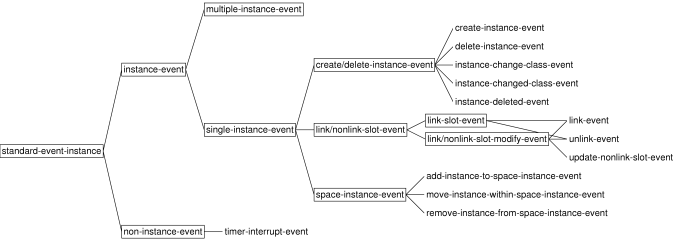
\includegraphics[scale=0.85]{gbbopen-events}
\end{center}
\W\end{iftex}

\noindent The event classes shown within rectangles are abstract classes
that cannot be signaled.

\W\xml{p}

Here are the defined event subclasses when both the \code{:gbbopen-core} and
\code{:agenda-shell} \glref{modules} have been loaded:
%
\T\begin{ifhtml}
\xml{br}
\xml{img align="center" src="agenda-shell-events.png"}
\xml{br clear="both"}
\T\end{ifhtml}
\W\begin{iftex} 
\begin{center}
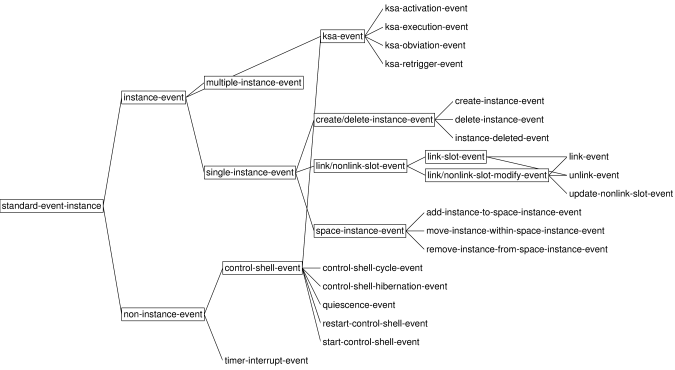
\includegraphics[scale=0.85]{agenda-shell-events}
\end{center}
\W\end{iftex}
%
The additional \code{control-shell-event} classes are defined and signaled by
the Agenda Shell.  Again classes shown within rectangles are abstract classes
that cannot be signaled.

\W\entities
\T\clearpage

%% ------------------------------------------------------------------------

\begin{functiondoc}{Function}{add-event-function}%
  {\var{function\/} [\var{event-class-specifier\/} 
    [\var{unit-class-or-instance-specifier\/}]] \\
    \code{\&key} \var{slot-names paths permanent priority\/}}
\index{event function!adding}%

%% Although the [] syntax is normally used for macros to denote optional
%% arguments, here we use them rather than &optional because of the 
%% keyword-driven argument parsing used in this function.

\fnsyntax

\fnpurpose Add an \glref{event~function} for one or more \glref{event~classes}.

\fnpackage \code{:gbbopen}

\fnmodule \code{:gbbopen-core}

\fnargs
\begin{args}{unit-class-or-instance-specifier}
\arg[function] A \glref{function~designator}
\arg[event-class-specifier] An \glref{extended~event-class~specification} 
(see below; default is \code{t})
\arg[unit-class-or-instance-specifier] An 
\glref{extended~unit-class~or~instance~specification} 
(see below; default is \code{t})
\arg[slot-names\/ \textrm{or} slot-name \T\hfil] A slot-name or list
of slot-names (default is \code{t})
\arg[paths\/ \textrm{or} path \T\hfil] A \glref{space-instance~path}
regular expression 
(default is \code{(*)})
\arg[permanent] A \glref{generalized~boolean} (default is \nil)
\arg[priority] An integer between -127 and 127, inclusive (default is \code{0})
\end{args}

\fndsyntax
\W\supp\tabletop
\eventclassspec
\subeventingspec
\syntaxsep
\unitclassinstancespec
\subclassingspec

\fndescription 
The specified \var{function\/} must accept the arguments associated with every
\glref{event~class} to which it is added.  In addition, \var{function\/}
should accept additional arguments that are associated with all
\glref{subevents} of the specified \glref{event~classes}. (This can be
achieved by specifying \code{\&allow-other-keys} in the lambda list of
\var{function}.)

The \var{paths\/} argument is either the symbol \code{t} (indicating
all \glref{space~instances}) or a list representing a regular
expression where the following reserved symbols are interpreted as
follows:
\spaceinstanceregexp

\begin{alsos}{remove-all-event-functions}
\also[remove-event-function]
\also[remove-all-event-functions]
\end{alsos}

\fnexamples
\bfindexit{evfn-printer}%
Add the event \glref{function} \entlink{evfn-printv} to the set of functions
to be invoked when \code{create-instance-event} is signaled on a
\code{hyp} \glref{unit~instance}:
%
\W\supp
\begin{example}
  (add-event-function 'evfn-printv 'create-instance-event 'hyp)
\end{example}
%
Add the event \glref{function} \entlink{evfn-printv} to the set of functions
to be invoked when \code{create-instance-event} is signaled on a
\code{hyp} \glref{unit~instance} or its subclasses:
%
\W\supp\notpretop
\begin{example}
  (add-event-function 'evfn-printv 'create-instance-event '(hyp :plus-subclasses))
\end{example}

\fnnote
\instanceevfnsnyi

\end{functiondoc}

%% ------------------------------------------------------------------------

\begin{functiondoc}{Macro}{define-event-class}{\var{event-class-name\/} 
   \code{(}\{\var{superclass-name\/}\}\superstar\code{)}
   [\var{documentation\/}] \\
   \code{(}\{\var{slot-specifier\/}\}\superstar\code{)}
   \{\var{class-option\/}\}\superstar{} 
   \returns{} \var{new-event-class\/}}
\index{event class!defining/redefining}%
\index{defining!an event class}%
\index{redefining!an event class}%

\fnsyntax

\fnpurpose Define or redefine an \glref{event~class}.

\fnpackage \code{:gbbopen}

\fnmodule \code{:gbbopen-core}

\fnargs
\begin{args}{event-class-name}
\arg[event-class-name] A non-\nil, \glref{non-keyword~symbol} that names the
\glref{event~class} 
\arg[superclass-name] A non-\nil, \glref{non-keyword~symbol} that specifies a
direct superclass of the \glref{event~class} \var{event-class-name\/}  
\arg[documentation] A documentation string
\arg[slot-specifiers] See below
\arg[class-options] See below
\arg[new-event-class] A new or modified \glref{event~class} object. 
\end{args}

\fnreturns The newly defined or modified \glref{event~class} object. 

\fndsyntax
\W\supp\tabletop
\begin{tabular}{@{~}l@{~}l}
\mbox{\var{slot-specifier\/} ::=}
 & \var{slot-name\/} \vbar{}
   \code{(}\var{slot-name\/} [[\var{slot-option\/}]]\code{)} \\
\end{tabular}
\T\\
\begin{tabular}{@{~}l@{~}l}
\mbox{\var{slot-option\/} ::=}
 & \{\code{:accessor} \var{reader-function-name\/}\}\superstar{} \vbar \\
 & \{\code{:allocation} \var{allocation-type\/}\} \vbar \\
 & \{\code{:documentation} \var{string\/}\} \vbar \\
 & \{\code{:initarg} \var{initarg-name\/}\}\superstar{} \vbar \\
 & \{\code{:initform} \var{form\/}\} \vbar \\
 & \{\code{:reader} \var{reader-function-name\/}\}\superstar{} \vbar \\
 & \{\code{:type} \var{type-specifier\/}\} \vbar{} \\
 & \{\code{:writer} \var{writer-function-name\/}\}\superstar{} \\
\end{tabular}
\T\\
\begin{tabular}{@{~}l@{~}l}
\mbox{\var{class-option\/} ::=}
 & \code{(:abstract} \var{boolean\/}\code{)} \vbar \\
 & \code{(:default-initargs .} \var{initarg-list\/}\code{)} \vbar \\
 & \code{(:documentation} \var{string\/}\code{)} \vbar \\
 & \code{(:event-metaclass} \var{event-metaclass-specifier\/}\code{)} \vbar \\
 & \code{(:event-printing} \var{event-printing-specifier\/}/code{)} \vbar \\
 & \code{(:export-class-name} \var{boolean\/}\code{)} \vbar \\
 & \code{(:export-accessors} \var{boolean\/}\code{)} \vbar \\
 & \code{(:generate-accessors} \var{direct-slots-specifier\/}\code{)} \vbar \\
 & \code{(:generate-accessors-format} 
     \{\code{:prefix} \vbar{} \code{:suffix}\} \vbar \\
 & \code{(:generate-accessors-prefix} \{\var{string\/} \vbar{}
     \var{symbol\/}\}\var\code{)} \vbar \\
 & \code{(:generate-accessors-suffix} \{\var{string\/} \vbar{}
     \var{symbol\/}\}\var\code{)} \vbar \\
 & \code{(:generate-initargs} \var{direct-slots-specifier\/}\code{)} \vbar \\
 & \code{(:metaclass} \var{class-name\/}\code{)} \\
\end{tabular}
\T\\
\begin{tabular}{@{~}l@{~}l}
\mbox{\var{event-metaclass-specifier\/} ::=}
  & non-instance-event-class \vbar{} instance-event-class \vbar{} \\
  & space-instance-event-class \vbar{} \\
  & nonlink-slot-event-class \vbar{} link-slot-event-class \\
\end{tabular}
\T\\
\begin{tabular}{@{~}l@{~}l}
\mbox{\var{direct-slots-specifier\/} ::=} & \nil{} \vbar{} \code{t} \vbar{}
  \var{included-slot-name\/}\superstar{} \vbar \\
  & \{\code{t :exclude} \var{excluded-slot-name\/}\superstar{}\} \\
\end{tabular}

\fnterms
\begin{args}{class-name}
\arg[class-name] A non-\nil, \glref{non-keyword~symbol} that names a
\glref{class} 
\arg[initarg-list] An \glref{initialization~argument~list}
\arg[slot-name] A non-\nil, \glref{non-keyword~symbol}
\end{args}

\fndescription 
\bfindexit{standard-event-class}%
Each \var{superclass-name} argument specifies a direct superclass of the new
class. If the superclass list is empty, then the direct superclass defaults to the
single class \textbf{\entlink{standard-event-instance}}.

\bfindexit{standard-event-class}%
The \code{:metaclass} \var{class-name\/} class option, if specified, must be a
subclass of \textbf{\entlinknoex{standard-event-class}}.  The default
metaclass value is the metaclass of the event superclasses of
\var{event-class-name} if they all have the same metaclass.  If the event
superclasses have multiple metaclasses, the metaclass of
\var{event-class-name} must be provided. The following table lists the
compatible event-superclass metaclasses for each \glref{event~metaclass}:

\begin{center}
\begin{tabular}{@{}l@{}l@{}c@{}l@{}c@{}l@{}c@{}l@{}c@{}l@{}c@{}}
& & \multicolumn{9}{c}{\textbf{Compatible Event-Superclass Metaclasses}}\\[4pt]
\multicolumn{1}{c}{\textbf{Event}}&~~~~~~&\code{non-}&~~&&~~&\code{space-}&~~& 
  \code{nonlink-}&~~&\code{link-}\\
\multicolumn{1}{c}{\textbf{Metaclass}}&&\code{instance}&&\code{instance}&&
   \code{instance}&&\code{slot}&&\code{slot}\\[4pt]
\code{non-instance-event-class}
   &&\textbf{X}&&          &&          &&          &&          \\
\code{instance-event-class}
   &&\textbf{X}&&\textbf{X}&&          &&          &&          \\
\code{space-instance-event-class}
   &&\textbf{X}&&\textbf{X}&&\textbf{X}&&          &&          \\
\code{nonlink-slot-event-class}
   &&\textbf{X}&&\textbf{X}&&          &&\textbf{X}&&          \\
\code{link-slot-event-class}
   &&\textbf{X}&&\textbf{X}&&          &&          &&\textbf{X}\\
\end{tabular}
\end{center}

The table in the documentation for \textbf{signal-event}
lists the \glref{initialization~arguments} that are required when
signaling an event.  These required \glref{initialization~arguments}
are based on the \glref{event~metaclass} of the \glref{event~class} of
the \glref{event} that is being signaled.

\begin{alsos}{with-generate-accessors-format}
\also[signal-event]
\also[standard-event-class]
\also[standard-event-instance]
\also[with-generate-accessors-format]
\end{alsos}

\bfindexit{non-instance-event}%
\fnexample
%
\W\supp
\begin{example}
> (define-event-class my-event (non-instance-event)
    ((my-event-arg1 :initform nil)
     (my-event-arg2 :initform nil)))
#<non-instance-event-class my-event>
\end{example}

\end{functiondoc}

%% ------------------------------------------------------------------------

\begin{functiondoc}{Function}{describe-event-printing}%
  {[\var{event-class-specifier\/} 
    [\var{unit-class-or-instance-specifier\/}]] \\
    \code{\&key} \var{slot-names paths\/}}
\index{event printing!printing information about}%
\index{printing!information about!event printing}%

%% Although the [] syntax is normally used for macros to denote optional
%% arguments, here we use them rather than &optional because of the 
%% keyword-driven argument parsing used in this function.

\fnsyntax

\fnpurpose Describe the printing of events for one or more
\glref{event~classes}. 

\fnpackage \code{:gbbopen}

\fnmodule \code{:gbbopen-core}

\fnargs
\begin{args}{unit-class-or-instance-specifier}
\arg[event-class-specifier] An \glref{extended~event-class~specification} 
(see below; default is \code{t})
\arg[unit-class-or-instance-specifier] An 
\glref{extended~unit-class~or~instance~specification} 
(see below; default is \code{t})
\arg[slot-names\/ \textrm{or} slot-name \T\hfil] A slot-name or list of
slot-names (default is \code{t})
\arg[paths\/ \textrm{or} path \T\hfil] A \glref{space-instance~path} regular
expression (default is \code{(*)})
\end{args}

\fndsyntax
\W\supp\tabletop
\eventclassspec
\subeventingspec
\syntaxsep
\unitclassinstancespec
\subclassingspec

\fndescription 
\bfindexit{*standard-output*}%
The \var{paths\/} argument is either the symbol \code{t} (indicating
all \glref{space~instances}) or a list representing a regular
expression where the following reserved symbols are interpreted as
follows:
\spaceinstanceregexp
The description is printed to the {\bf *standard-output*} stream.

\begin{alsos}{suspend-event-printing}
\also[disable-event-printing]
\also[enable-event-printing]
\also[resume-event-printing]
\also[suspend-event-printing]
\end{alsos}

\fnexample
Describe all event printing:
%
\W\supp
\begin{example}
> (describe-event-printing 'instance-event)
instance-event
  standard-unit-instance
  uc-2 [suspended]
  uc-1 [suspended]
  ksa
  ks
  root-space-instance
  standard-space-instance
\end{example}

\fnnote
\instanceevfnsnyi

\end{functiondoc}

%% ------------------------------------------------------------------------

\begin{functiondoc}{Function}{disable-event-printing}%
  {[\var{event-class-specifier\/} 
    [\var{unit-class-or-instance-specifier\/}]] \\
    \code{\&key} \var{slot-names paths\/}}
\index{event printing!disabling}%
\index{disabling!event printing}%

%% Although the [] syntax is normally used for macros to denote optional
%% arguments, here we use them rather than &optional because of the 
%% keyword-driven argument parsing used in this function.

\fnsyntax

\fnpurpose Disable the printing of events for one or more
\glref{event~classes}. 

\fnpackage \code{:gbbopen}

\fnmodule \code{:gbbopen-core}

\fnargs
\begin{args}{unit-class-or-instance-specifier}
\arg[event-class-specifier] An \glref{extended~event-class~specification} 
(see below; default is \code{t})
\arg[unit-class-or-instance-specifier] An 
\glref{extended~unit-class~or~instance~specification} 
(see below; default is \code{t})
\arg[slot-names\/ \textrm{or} slot-name \T\hfil] A slot-name or list of slot-names
(default is \code{t})
\arg[paths\/ \textrm{or} path \T\hfil] A \glref{space-instance~path} regular expression
(default is \code{(*)})
\end{args}

\fndsyntax
\W\supp\tabletop
\eventclassspec
\subeventingspec
\syntaxsep
\unitclassinstancespec
\subclassingspec

\fndescription 
The \var{paths\/} argument is either the symbol \code{t} (indicating
all \glref{space~instances}) or a list representing a regular
expression where the following reserved symbols are interpreted as
follows:
\spaceinstanceregexp

\begin{alsos}{describe-event-printing}
\also[describe-event-printing]
\also[enable-event-printing]
\also[resume-event-printing]
\also[suspend-event-printing]
\end{alsos}

\fnexample
Disable all event printing:
%
\W\supp
\begin{example}
  (disable-event-printing)
\end{example}

\fnnote
\instanceevfnsnyi

\end{functiondoc}

%% ------------------------------------------------------------------------

\begin{functiondoc}{Function}{enable-event-printing}%
{[\var{event-class-specifier\/} 
[\var{unit-class-or-instance-specifier\/}]] \\
\code{\&key} \var{slot-names paths\/}}
\index{event printing!enabling}%

%% Although the [] syntax is normally used for macros to denote optional
%% arguments, here we use them rather than &optional because of the 
%% keyword-driven argument parsing used in this function.

\fnsyntax

\fnpurpose Enable the printing of events for one or more \glref{event~classes}.

\fnpackage \code{:gbbopen}

\fnmodule \code{:gbbopen-core}

\fnargs
\begin{args}{unit-class-or-instance-specifier}
\arg[event-class-specifier] An \glref{extended~event-class~specification} 
(see below; default is \code{t})
\arg[unit-class-or-instance-specifier] An 
\glref{extended~unit-class~or~instance~specification} 
(see below; default is \code{t})
\arg[slot-names\/ \textrm{or} slot-name \T\hfil] A slot-name or list of slot-names
(default is \code{t})
\arg[paths\/ \textrm{or} path \T\hfil] A \glref{space-instance~path} regular expression
(default is \code{(*)})
\end{args}

\fndsyntax
\W\supp\tabletop
\eventclassspec
\subeventingspec
\syntaxsep
\unitclassinstancespec
\subclassingspec

\fndescription 
The \var{paths\/} argument is either the symbol \code{t} (indicating
all \glref{space~instances}) or a list representing a regular
expression where the following reserved symbols are interpreted as
follows:
\spaceinstanceregexp

\begin{alsos}{describe-event-printing}
\also[describe-event-printing]
\also[disable-event-printing]
\also[resume-event-printing]
\also[suspend-event-printing]
\end{alsos}

\fnexample
Enable event printing on all \glref{space-instance} events of
\code{hyp} \glref{unit~instances}:
%
\W\supp
\begin{example}
  (enable-event-printing '(space-instance-event :plus-subevents)
                         '(hyp :plus-subclasses))
\end{example}

\fnnote
\instanceevfnsnyi

\end{functiondoc}

%% ------------------------------------------------------------------------

\begin{functiondoc}{Function}{evfn-printv}{\var{event-class\/} 
    \&rest \var{args\/}}
\index{debugging, using evfn-printv@using \textbf{evfn-printv}}% 

\fnsyntax

\fnpurpose Assist debugging by printing forms and the results of
evaluating them to \code{*trace-output*}.

\fnpackage \code{:gbbopen}

\fnmodule \code{:gbbopen-core}

\fnargs
\begin{args}{results}
\arg[forms] An implicit \textbf{progn} of \glref{forms} to be
evaluated and printed  
\end{args}

\fnreturns The values returned by evaluating the last \var{form}.

\fndescription Evaluates \var{forms\/}, printing the \var{form\/} and the
result values of each evaluation to \code{*trace-output*}.  Any\var{form\/}
that is a string (before evaluation) is simply printed without enclosing
double-quote characters.

\fnexamples
\bfindexit{evfn-printer}%
Add the event \glref{function} \entlink{evfn-printv} to the set of functions
to be invoked when \code{create-instance-event} is signaled on a
\code{hyp} \glref{unit~instance}:
%
\W\supp
\begin{example}
  (add-event-function 'evfn-printv 'create-instance-event 'hyp)
\end{example}

\end{functiondoc}

%% ------------------------------------------------------------------------

\begin{functiondoc}{Function}{remove-all-event-functions}%
{[\var{event-class-specifier\/} 
[\var{unit-class-or-instance-specifier\/}]] \\
\code{\&key} \var{slot-names paths permanent\/}}
\index{event function!removing all}%

%% Although the [] syntax is normally used for macros to denote optional
%% arguments, here we use them rather than &optional because of the 
%% keyword-driven argument parsing used in this function.

\fnsyntax

\fnpurpose Remove all \glref{event~functions} for one or more \glref{event~classes}.

\fnpackage \code{:gbbopen}

\fnmodule \code{:gbbopen-core}

\fnargs
\begin{args}{unit-class-or-instance-specifier}
\arg[event-class-specifier] An \glref{extended~event-class~specification} 
(see below; default is \code{t})
\arg[unit-class-or-instance-specifier] An 
\glref{extended~unit-class~or~instance~specification}
(see below; default is \code{t})
\arg[slot-names\/ \textrm{or} slot-name \T\hfil] A slot-name or list of slot-names
(default is \code{t})
\arg[paths\/ \textrm{or} path \T\hfil] A \glref{space-instance~path} regular expression
(default is \code{(*)})
\arg[permanent] A \glref{generalized~boolean} (default is \nil)
\end{args}

\fndsyntax
\W\supp\tabletop
\eventclassspec
\subeventingspec
\syntaxsep
\unitclassinstancespec
\subclassingspec

\begin{alsos}{remove-event-function}
\also[add-event-function]
\also[remove-event-function]
\end{alsos}

\fnexamples
\bfindexit{evfn-printer}%
Remove all event functions associated with a
\code{create-instance-event} on a \code{hyp} \glref{unit~instance}:
%
\W\supp
\begin{example}
  (remove-all-event-functions 'create-instance-event 'hyp)
\end{example}
%
Remove all event functions associated with a
\code{create-instance-event} on a \code{hyp} \glref{unit~instance} or
its subclasses:
%
\W\supp\notpretop
\begin{example}
  (remove-all-event-functions 'create-instance-event '(hyp :plus-subclasses))
\end{example}

\fnnote
\instanceevfnsnyi

\end{functiondoc}

%% ------------------------------------------------------------------------

\begin{functiondoc}{Function}{remove-event-function}%
{\var{function\/} [\var{event-class-specifier\/} 
[\var{unit-class-or-instance-specifier\/}]] \\
\code{\&key} \var{slot-names paths permanent\/}}
\index{event function!removing}%

%% Although the [] syntax is normally used for macros to denote optional
%% arguments, here we use them rather than &optional because of the 
%% keyword-driven argument parsing used in this function.

\fnsyntax

\fnpurpose Remove an \glref{event~function} for one or more \glref{event~classes}.

\fnpackage \code{:gbbopen}

\fnmodule \code{:gbbopen-core}

\fnargs
\begin{args}{space-instance}
\arg[function] A \glref{function~designator}
\arg[event-class-specifier] An \glref{extended~event-class~specification} 
(see below; default is \code{t})
\arg[unit-class-or-instance-specifier] An 
\glref{extended~unit-class~or~instance~specification}
(see below; default is \code{t})
\arg[slot-names\/ \textrm{or} slot-name \T\hfil] A slot-name or list of slot-names
(default is \code{t})
\arg[paths\/ \textrm{or} path \T\hfil] A \glref{space-instance~path} regular expression
(default is \code{(*)})
\arg[permanent] A \glref{generalized~boolean} (default is \nil)
\end{args}

\fndsyntax
\W\supp\tabletop
\eventclassspec
\subeventingspec
\syntaxsep
\unitclassinstancespec
\subclassingspec

\begin{alsos}{remove-all-event-functions}
\also[add-event-function]
\also[remove-all-event-functions]
\end{alsos}

\fnexamples
\bfindexit{evfn-printer}%
Remove the event \glref{function} \entlink{evfn-printv} from the set of functions
to be invoked when \code{create-instance-event} is signaled on a
\code{hyp} \glref{unit~instance}:
%
\W\supp
\begin{example}
  (remove-event-function 'evfn-printv 'create-instance-event 'hyp)
\end{example}
%
Remove the event \glref{function} \entlink{evfn-printv} from the set of
functions to be invoked when \code{create-instance-event} is signaled on a
\code{hyp} \glref{unit~instance} or its subclasses:
%
\W\supp\notpretop
\begin{example}
  (remove-event-function 'evfn-printv 'create-instance-event '(hyp :plus-subclasses))
\end{example}

\fnnote
\instanceevfnsnyi

\end{functiondoc}

%% ------------------------------------------------------------------------

\begin{functiondoc}{Function}{resume-event-printing}%
{[\var{event-class-specifier\/} 
[\var{unit-class-or-instance-specifier\/}]] \\
\code{\&key} \var{slot-names paths\/}}
\index{event printing!resuming}%

%% Although the [] syntax is normally used for macros to denote optional
%% arguments, here we use them rather than &optional because of the 
%% keyword-driven argument parsing used in this function.

\fnsyntax

\fnpurpose Resume the printing of printing-enabled events for one or more
\glref{event~classes}. 

\fnpackage \code{:gbbopen}

\fnmodule \code{:gbbopen-core}

\fnargs
\begin{args}{unit-class-or-instance-specifier}
\arg[event-class-specifier] An \glref{extended~event-class~specification} 
(see below; default is \code{t})
\arg[unit-class-or-instance-specifier] An 
\glref{extended~unit-class~or~instance~specification} 
(see below; default is \code{t})
\arg[slot-names\/ \textrm{or} slot-name \T\hfil] A slot-name or list of slot-names
(default is \code{t})
\arg[paths\/ \textrm{or} path \T\hfil] A \glref{space-instance~path} regular expression
(default is \code{(*)})
\end{args}

\fndsyntax
\W\supp\tabletop
\eventclassspec
\subeventingspec
\syntaxsep
\unitclassinstancespec
\subclassingspec

\fndescription 
The \var{paths\/} argument is either the symbol \code{t} (indicating
all \glref{space~instances}) or a list representing a regular
expression where the following reserved symbols are interpreted as
follows:
\spaceinstanceregexp

\begin{alsos}{describe-event-printing}
\also[describe-event-printing]
\also[disable-event-printing]
\also[enable-event-printing]
\also[suspend-event-printing]
\end{alsos}

\fnexample
Resume all suspended event printing:
%
\W\supp
\begin{example}
  (resume-event-printing)
\end{example}

\fnnote
Resuming event printing does not enable event printing that is disabled.

\instanceevfnsnyi

\end{functiondoc}

%% ------------------------------------------------------------------------

\begin{functiondoc}{Function}{signal-event}{\var{event-class\/}
  \code{\&rest} \var{initargs\/}}
\index{event!signaling}%
\index{signaling!an event}%

\fnsyntax

\fnpurpose Signal an event

\fnpackage \code{:gbbopen}

\fnmodule \code{:gbbopen-core}

\fnargs
\begin{args}{initargs}
\arg[event-class] An \glref{event~class} or a non-\nil, \glref{non-keyword~symbol} that 
names an \glref{event~class} 
\arg[initargs] An \glref{initialization~argument~list}
\end{args}

\fndescription

\index{event function!required arguments}%
\index{function!event!required arguments}%
The following table lists the \glref{initialization~arguments} that
are required for specific event metaclasses:
\begin{center}
  \begin{tabular}{@{}l@{}l@{}}
  \textbf{Event metaclass} & \textbf{Required initargs} \\ \hline
  \code{non-instance-event-class} 
  & None \\
  \code{instance-event-class} 
  & \code{:instance} \var{unit-instance\/} \\
  \code{space-instance-event-class}~~~~~
  & \code{:instance} \var{unit-instance\/} \\
  & \code{:space-instance} \var{space-instance\/} \\ 
  \code{nonlink-slot-event-class}
  & \code{:instance} \var{unit-instance\/} \\
  & \code{:slot} \var{effective-nonlink-slot-definition\/} \\
  \code{link-slot-event-class}
  & \code{:instance} \var{unit-instance\/} \\
  & \code{:slot} \var{effective-link-definition\/} \\ \hline
\end{tabular}
\end{center}

\begin{alsos}{with-events-disabled}
\also[define-event-class]
\also[with-events-disabled]
\also[with-events-enabled]
\end{alsos}

\fnexample
%
\W\supp
\begin{example}
  (signal-event 'my-event :my-event-arg1 3)
\end{example}
\end{functiondoc}

%% ------------------------------------------------------------------------

\begin{functiondoc}{Class}{standard-event-class}{}
\index{class!standard-event-class@\textbf{standard-event-class}}%

\fnsyntax

\fnpackage \code{:gbbopen}

\fnmodule \code{:gbbopen-core}

\fndescription 
\bfindexit{define-event-class}%
The class \textbf{standard-event-class} is the superclass of classes defined
by \textbf{\entlinknoex{define-event-class}}.  It is a subclass of
\code{standard-class}.

\begin{alsos}{standard-event-instance}
\also[define-event-class]
\also[standard-event-instance]
\end{alsos}

\end{functiondoc}

%% ------------------------------------------------------------------------

\begin{functiondoc}{Event~Class}{standard-event-instance}{}
\index{class!standard-event-instance@\textbf{standard-event-instance}}%
\index{event class!standard-event-instance@\textbf{standard-event-instance}}%
  
\fnsyntax

\fnpackage \code{:gbbopen}

\fnmodule \code{:gbbopen-core}

\fndescription 
\bfindexit{standard-event-class}%
The class \textbf{standard-event-instance} is an \glref{instance} of
\textbf{\entlinknoex{standard-event-class}} and is a superclass of every
\glref{event~class} that is an \glref{instance} of
\textbf{\entlinknoex{standard-event-class}} except itself.  It is a subclass
of \textbf{\glref{standard-gbbopen-instance}}.

\begin{alsos}{standard-event-class}
\also[print-instance-slots]
\also[standard-gbbopen-instance]
\also[standard-event-class]
\end{alsos}

\end{functiondoc}

%% ------------------------------------------------------------------------

\begin{functiondoc}{Function}{suspend-event-printing}%
{[\var{event-class-specifier\/} 
[\var{unit-class-or-instance-specifier\/}]] \\
\code{\&key} \var{slot-names paths\/}}
\index{event printing!suspending}%

%% Although the [] syntax is normally used for macros to denote optional
%% arguments, here we use them rather than &optional because of the 
%% keyword-driven argument parsing used in this function.

\fnsyntax

\fnpurpose Suspend the printing of printing-enabled events for one or more
\glref{event~classes}. 

\fnpackage \code{:gbbopen}

\fnmodule \code{:gbbopen-core}

\fnargs
\begin{args}{unit-class-or-instance-specifier}
\arg[event-class-specifier] An \glref{extended~event-class~specification} 
(see below; default is \code{t})
\arg[unit-class-or-instance-specifier] An 
\glref{extended~unit-class~or~instance~specification} 
(see below; default is \code{t})
\arg[slot-names\/ \textrm{or} slot-name \T\hfil] A slot-name or list of slot-names
(default is \code{t})
\arg[paths\/ \textrm{or} path \T\hfil] A \glref{space-instance~path} regular expression
(default is \code{(*)})
\end{args}

\fndsyntax
\W\supp\tabletop
\eventclassspec
\subeventingspec
\syntaxsep
\unitclassinstancespec
\subclassingspec

\fndescription 
Suspending event printing is a convenient way of switching off event
printing without losing event-printing enabled/disabled settings.
Disabled event printing remains disabled if event printing is
resumed (by using \textbf{\entlinknoex{resume-event-printing}}).

The \var{paths\/} argument is either the symbol \code{t} (indicating
all \glref{space~instances}) or a list representing a regular
expression where the following reserved symbols are interpreted as
follows:
\spaceinstanceregexp

\begin{alsos}{describe-event-printing}
\also[describe-event-printing]
\also[disable-event-printing]
\also[enable-event-printing]
\also[resume-event-printing]
\end{alsos}

\fnexample
Suspend all event printing associated with \code{possible-hyp}
\glref{unit~instances}: 
%
\W\supp
\begin{example}
  (suspend-event-printing 't 'possible-hyp)
\end{example}

\fnnote
\instanceevfnsnyi

\end{functiondoc}

%% ------------------------------------------------------------------------

\begin{functiondoc}{Macro}{with-events-disabled}%
  {\code{(}\var{option\/}\superstar{}\code{)}
    \var{declaration\/}\superstar{}
    \var{form\/}\superstar{}
    \returns{} \var{result\/}\superstar}
\index{disabling!event signaling}%
\index{events!disabling signaling of}%
  
\fnsyntax

\fnpurpose Disable event signaling during evaluation of \var{forms}.

\fnpackage \code{:gbbopen}

\fnmodule \code{:gbbopen-core}

\fnargs
\begin{args}{options}
\arg[option] No options are currently supported
\arg[declaration] A declare expression
\arg[forms] An implicit \textbf{progn} of \glref{forms} to be evaluated
\arg[results] The values returned by evaluating the last \var{form}
\end{args}

\fnreturns The values returned by evaluating the last \var{form}.

\begin{alsos}{with-events-enabled}
\also[signal-event]
\also[with-events-enabled]
\end{alsos}

\fnexample
\bfindexit{make-instance}%
Create a \code{hyp} without signaling any events:
%
\W\supp
\begin{example}
> (with-events-disabled ()
     (\entlink{make-instance} 'hyp 
        :location (list x y)
        :classification '(:car :truck)
        :color ':red
        :belief .85
        :velocity-range '(5 35)
        :supporting-hyps supporting-hyps))
#<hyp 419 (1835 4791) 0.85 [5..35]>
\end{example}

\end{functiondoc}

%% ------------------------------------------------------------------------

\begin{functiondoc}{Macro}{with-events-enabled}%
  {\code{(}\var{option\/}\superstar{}\code{)}
    \var{declaration\/}\superstar{}
    \var{form\/}\superstar{}
    \returns{} \var{result\/}\superstar}
\index{enabling event signaling}%
\index{events!enabling signaling of}%
  
\fnsyntax

\fnpurpose Restore event signaling during evaluation of \var{forms}.

\fnpackage \code{:gbbopen}

\fnmodule \code{:gbbopen-core}

\fnargs
\begin{args}{options}
\arg[option] No options are currently supported
\arg[declaration] A declare expression
\arg[forms] An implicit \textbf{progn} of \glref{forms} to be evaluated
\arg[results] The values returned by evaluating the last \var{form}
\end{args}

\fnreturns The values returned by evaluating the last \var{form}.

\begin{alsos}{with-events-disabled}
\also[signal-event]
\also[with-events-disabled]
\end{alsos}

\fnexample
\bfindexit{make-instance}%
Create a \code{hyp} without signaling any events, then add
supporting-hypothesis links with events enabled:
%
\W\supp
\begin{example}
> (\entlink{with-events-disabled}
     (let ((hyp (\entlink{make-instance} 'hyp 
                   :location (list x y)
                   :classification '(:car :truck)
                   :color ':red
                   :belief .85
                   :velocity-range '(5 35))))
        (with-events-enabled ()
           (linkf (supporting-hyps-of hyp) supporting-hyps))
        hyp))
#<hyp 419 (1835 4791) 0.85 [5..35]>
\end{example}

\end{functiondoc}

%% ------------------------------------------------------------------------

\T\markright{}%
\T\pagestyle{plain}
\T\clearpage
\W\xname{ref-interval-entities}
\T\pagestyle{fancy}
\T\thispagestyle{fancybottom}
\T\global\def\fnlastname{ }%

\subsection{Intervals}
\label{sec:interval}%

This section contains \code{:gbbopen-core} entities that pertain to
\glref{intervals}. An interval $[a,b]$ is the set of real numbers between the
start value of the interval, $a$, and the end value, $b$, inclusive. The
interval $[x,x]$ represents the single point $x$.

An interval is represented as either a \glref{cons}, a two-element list, or a
two-element array containing the start and end values of the interval.  So, a
representation for the interval $[0,100]$ can be created as any of the
following:
\begin{tightitemize}
\item \code{(cons 0 100)}
\item \code{(list 0 100)}
\item \code{(vector 0 100)}
\end{tightitemize}
%
The function \textbf{\entlink{make-interval}} is provided for stylistic
clarity in creating an interval.

\bfindexit{make-interval}%
%
Intervals also include the unbounded intervals:
\begin{tightitemize}
\item $(-\infty,\infty)$ ~ (provided as the constant 
  \textbf{\entlink{infinite-interval}})
\item $(-\infty,x]$      ~ (for example, 
   \code{(\entlink{make-interval} x infinity)})
\item $[x,\infty)$       ~ (for example, 
   \code{(\entlink{make-interval} -infinity x)})
\end{tightitemize}

It is an error for the start value of an interval to be greater than the end
value.

\W\entities
\T\clearpage

%% ------------------------------------------------------------------------

\begin{functiondoc}[coerce-contracted-interval-rationals-to-floats-var]%
  {Variable}%
  {*coerce-contracted-interval-rationals-to-floats*}{}%

\fnsyntax

\fnpurpose Control automatic coercion of non-integer rationals to floats when
an interval is contracted into a non-integral point range by
\textbf{\entlink{expand-interval}} and \textbf{\entlink{nexpand-interval}}.

\fnpackage \code{:gbbopen}

\fnmodule \code{:gbbopen-core}

\fnvaluetype A \glref{generalized~boolean}

\fninitialvalue \nil{}

\begin{alsos}{nexpand-interval}
\also[expand-interval]
\also[nexpand-interval]
\end{alsos}

\fnexamples
%
\bfindexit{expand-interval}%
%
\W\supp
\begin{example}
> (let ((*coerce-contracted-interval-rationals-to-floats* 't))
     (expand-interval '(2 . 5) -3))
(3.5 . 3.5)
> (let ((*coerce-contracted-interval-rationals-to-floats* nil))
     (expand-interval '(2 . 5) -3))
(7/2 . 7/2)
>
\end{example}

\end{functiondoc}

%% ------------------------------------------------------------------------

\begin{functiondoc}{Function}{copy-interval}%
  {\var{interval\/}
    \returns{} \var{new-interval\/}}
\index{copy, an interval}%
\index{interval!copying}%

\fnsyntax

\fnpurpose Create a new \glref{interval} by copying \var{interval}.

\fnpackage \code{:gbbopen}

\fnmodule \code{:gbbopen-core}

\fnargs
\begin{args}{new-interval}
\arg[interval] An \glref{interval}
\arg[new-interval] An \glref{interval}
\end{args}

\fnreturns The new \glref{interval}.

\fndescription The structure of the original \var{interval\/} (\glref{cons},
two-element list, or two-element array) is maintained in the newly allocated
\var{new-interval}.

\begin{alsos}{infinite-interval}
\also[expand-interval]
\also[infinite-interval]
\also[interval-start]
\also[interval-end]
\also[make-interval]
\also[nexpand-interval]
\also[nshift-interval]
\also[shift-interval]
\end{alsos}

\fnexamples
%
\W\supp
\begin{example}
> (copy-interval '(2 5))
(2 5)
> (copy-interval '(2 . 5))
(2 . 5)
> (expand-interval #(2 5))
#(2 5)
\end{example}

\end{functiondoc}

%% ------------------------------------------------------------------------

\begin{functiondoc}{Function}{expand-interval}%
  {\var{interval amount\/}
    \returns{} \var{new-interval\/}}
\index{expand, an interval}%
\index{interval!expanding}%

\fnsyntax

\fnpurpose Create a new \glref{interval} by expanding \var{interval\/} by
\var{amount}.

\fnpackage \code{:gbbopen}

\fnmodule \code{:gbbopen-core}

\fnargs
\begin{args}{new-interval}
\arg[interval] An \glref{interval}
\arg[amount] A numbe
\arg[new-interval] An \glref{interval}
\end{args}

\fnreturns A new, expanded \glref{interval}.

\fndescription The structure of the original \var{interval\/}
(\glref{cons}, two-element list, or two-element array) is maintained in the
newly allocated, expanded \var{new-interval}.

An interval that is contracted (expanded negatively) by an amount greater than
one-half of its width will result in a zero-width \var{new-interval\/} at the
center point of the original \var{interval}.

\begin{alsos}{*coerce-contracted-interval-rationals-to-floats*}
\also[*coerce-contracted-interval-rationals-to-floats*]
\also[copy-interval]
\also[infinite-interval]
\also[interval-start]
\also[interval-end]
\also[interval-values]
\also[make-interval]
\also[nexpand-interval]
\also[nshift-interval]
\also[shift-interval]
\end{alsos}

\fnexamples
%
\W\supp
\begin{example}
> (expand-interval '(2 5) 2)
(0 7)
> (expand-interval '(2 . 5) -1)
(3 . 4)\goodpagebreak
> (expand-interval #(2 5) .5)
#(1.5 5.5)
> (expand-interval '(2 . 5) -3)
(3.5 . 3.5)
\end{example}

\end{functiondoc}

%% ------------------------------------------------------------------------

\begin{functiondoc}{Function}{expand-point}%
  {\var{point amount\/}
    \code{\&optional} \var{type-specifier\/} 
    \returns{} \var{new-interval\/}}
\index{expand, a point into an interval}%
\index{point!expanding into an interval}%

\fnsyntax

\fnpurpose Create a new \glref{interval} by expanding \var{point\/} by
\var{amount}.

\fnpackage \code{:gbbopen}

\fnmodule \code{:gbbopen-core}

\fnargs
\begin{args}{type-specifier}
\arg[point] A number
\arg[amount] A number
\arg[type-specifier] One of: \code{cons}, \code{list}, or \code{array}.
  (Default is \code{cons}.)
\arg[new-interval] An \glref{interval}
\end{args}

\fnreturns The new \glref{interval}.

\begin{alsos}{nexpand-interval}
\also[expand-interval]
\also[interval-start]
\also[interval-end]
\also[interval-values]
\also[make-interval]
\also[nexpand-interval]
\also[nshift-interval]
\also[shift-interval]
\end{alsos}

\fnexamples
%
\W\supp
\begin{example}
> (expand-point 3 2)
(1 . 5)
> (expand-point 3 2 'cons)
(1 . 5)
> (expand-point 3 2 'list)
(1 5)
> (expand-point 3 2 'array)
#(1 5)
\end{example}

\fnnote
%
\bfindex{expand-point\&}%
\bfindex{expand-point\$\&}%
\bfindex{expand-point\$}%
\bfindex{expand-point\$\$}%
\bfindex{expand-point\$\$\$}%
%
\reflink{Declared numeric}{sec:declared-numerics} versions of
\textbf{expand-point} are also provided: \textbf{expand-point\&},
\textbf{expand-point\$\&}, \textbf{expand-point\$},
\textbf{expand-point\$\$}, and \textbf{expand-point\$\$\$}.

\end{functiondoc}

%% ------------------------------------------------------------------------

\begin{functiondoc}{Constant}{infinite-interval}{}%

\fnsyntax

\fnpurpose An interval (represented as a cons) from \code{-infinity} to
\code{infinity}.

\fnpackage \code{:gbbopen}

\fnmodule \code{:gbbopen-core}

\begin{alsos}{nexpand-interval}
\also[copy-interval]
\also[expand-interval]
\also[interval-end]
\also[interval-start]
\also[interval-values]
\also[make-interval]
\also[nexpand-interval]
\also[nshift-interval]
\also[shift-interval]
\end{alsos}

\fnexample
%
\bfindexit{define-unit-class}%
\bfindexit{copy-interval}%
%
Define a \glref{unit~class}, \code{temporal-duration-mixin}, that contains a
\code{temporal-duration} slot and \glref{dimension~value} declaration:
%
\W\supp
\begin{example}
> (define-unit-class temporal-duration-mixin ()
    ((temporal-duration 
       ;; Copy the interval to allow destructive changes by
       ;; GBBopen's interval operators:
       :initform (copy-interval infinite-interval)))
    (:dimensional-values
     (temporal-duration :interval temporal-duration)))
#<standard-unit-class temporal-duration-mixin>
\end{example}

\end{functiondoc}

%% ------------------------------------------------------------------------

\begin{functiondoc}{Function}{interval-end}%
  {\var{interval\/}
    \returns{} \var{end-value\/}}
\index{end value, of an interval}%
\index{interval!obtaining the end value}%

\fnsyntax

\fnpurpose Obtain the end value of an \glref{interval}.

\fnsetf
\fnsetfsyntax{interval-end}{\var{interval\/}}{\var{end-value\/}}

\fnpackage \code{:gbbopen}

\fnmodule \code{:gbbopen-core}

\fnargs
\begin{args}{interval}
\arg[interval] An \glref{interval}
\arg[end-value] A number
\end{args}

\fnreturns The end value of the \glref{interval}.

\begin{alsos}{interval-values}
\also[interval-start]
\also[interval-values]
\end{alsos}

\fnexamples
%
\bfindexit{make-interval}
%
\W\supp
\begin{example}
> (interval-end '(1 2))
2
> (interval-end '(1 . 2))
2
> (interval-end #(1  2))
2\goodpagebreak
> (defparameter *x* (\entlink{make-interval} 1 2))
(1 . 2)
> (setf (interval-end *x*) 4)
4
> *x*
(1 . 4)
\end{example}

\end{functiondoc}

%% ------------------------------------------------------------------------

\begin{functiondoc}{Function}{interval-start}%
  {\var{interval\/} 
    \returns{} \var{start-value\/}}
\index{start value, of an interval}%
\index{interval!obtaining the start value}%

\fnsyntax

\fnpurpose Obtain the start value of an \glref{interval}.

\fnsetf
\fnsetfsyntax{interval-start}{\var{interval\/}}{\var{start-value\/}}

\fnpackage \code{:gbbopen}

\fnmodule \code{:gbbopen-core}

\fnargs
\begin{args}{interval}
\arg[interval] An \glref{interval}
\arg[start-value] A number
\end{args}

\fnreturns The start value of the \glref{interval}.

\begin{alsos}{interval-values}
\also[interval-end]
\also[interval-values]
\end{alsos}

\fnexamples
%
\bfindexit{make-interval}
%
\W\supp
\begin{example}
> (interval-start '(1 2))
1
> (interval-start '(1 . 2))
1
> (interval-start #(1 2))
1\goodpagebreak
> (defparameter *x* (\entlink{make-interval} 1 2))
(1 . 2)
> (setf (interval-start *x*) -1)
-1
> *x*
(-1 . 4)

\end{example}

\end{functiondoc}

%% ------------------------------------------------------------------------

\begin{functiondoc}{Function}{interval-values}%
  {\var{interval\/} 
    \returns{} \var{start-value, end-value\/}}
\index{start value, of an interval}%
\index{end value, of an interval}%
\index{values, start and end, of an interval}%
\index{interval!obtaining the start value}%
\index{interval!obtaining the end value}%
\index{interval!obtaining the start and end values}%

\fnsyntax

\fnpurpose Obtain the start and end values of an \glref{interval}.

\fnsetf
\fnsetfsyntax{interval-values}{\var{interval\/}}{\var{source-interval\/}}

\fnpackage \code{:gbbopen}

\fnmodule \code{:gbbopen-core}

\fnargs
\begin{args}{source-interval}
\arg[interval] An \glref{interval}
\arg[source-interval] An \glref{interval}
\arg[start-value] A number
\arg[end-value] A number
\end{args}

\fnreturns Two values: the start value and the end value of the \glref{interval}.

\begin{alsos}{interval-start}
\also[interval-end]
\also[interval-start]
\end{alsos}

\fnexamples
%
\bfindexit{make-interval}
%
\W\supp
\begin{example}
> (interval-values '(1 2))
1
2
> (interval-values '(1 . 2))
1
2
> (interval-values #(1  2))
1
2\goodpagebreak
> (defparameter *x* (\entlink{make-interval} 1 2))
(1 . 2)
> (setf (interval-values *x*) #(3 4))
#(3 4)
> *x*
(3 . 4)
\end{example}

\end{functiondoc}

%% ------------------------------------------------------------------------

\begin{functiondoc}{Function}{make-interval}%
  {\var{start end\/} 
    \code{\&optional} \var{type-specifier\/} 
    \returns{} \var{new-interval\/}}
\index{make, an interval}%
\index{interval!making}%

\fnsyntax

\fnpurpose Create a new \glref{interval} of type \var{type-specifier}.

\fnpackage \code{:gbbopen}

\fnmodule \code{:gbbopen-core}

\fnargs
\begin{args}{type-specifier}
\arg[start] A number
\arg[end] A number
\arg[type-specifier] One of: \code{cons}, \code{list}, or \code{array}.
  (Default is \code{cons}.)
\arg[new-interval] An \glref{interval}
\end{args}

\fnreturns The new \glref{interval}.

\begin{alsos}{infinite-interval}
\also[copy-interval]
\also[expand-interval]
\also[expand-point]
\also[infinite-interval]
\also[interval-start]
\also[interval-end]
\also[nexpand-interval]
\also[nshift-interval]
\also[shift-interval]
\end{alsos}

\fnexamples
%
\W\supp
\begin{example}
> (make-interval 2 5)
(2 . 5)
> (make-interval 2 5 'list)
(2 5)
> (make-interval 2 5 'cons)
(2 . 5)
> (make-interval 2 5 'array)
#(2 5)
\end{example}

\end{functiondoc}

%% ------------------------------------------------------------------------

\begin{functiondoc}{Function}{nexpand-interval}%
  {\var{interval amount\/}
    \returns{} \var{interval\/}}
\index{expand, an interval}%
\index{interval!expanding}%

\fnsyntax

\fnpurpose Expand an \glref{interval} by \var{amount}.

\fnpackage \code{:gbbopen}

\fnmodule \code{:gbbopen-core}

\fnargs
\begin{args}{interval}
\arg[interval] An \glref{interval}
\arg[amount] A number
\end{args}

\fnreturns The expanded \var{interval}.

\fndescription An interval that is contracted (expanded negatively) by an
amount greater than one-half of its width will result in a zero-width
\var{interval\/} at the center point of the original \var{interval}.

\begin{alsos}{*coerce-contracted-interval-rationals-to-floats*}
\also[*coerce-contracted-interval-rationals-to-floats*]
\also[copy-interval]
\also[expand-interval]
\also[expand-point]
\also[infinite-interval]
\also[interval-start]
\also[interval-values]
\also[interval-end]
\also[make-interval]
\also[nshift-interval]
\also[shift-interval]
\end{alsos}

\fnexamples
%
\W\supp
\begin{example}
> (nexpand-interval '(2 5) 2)
(0 7)
> (nexpand-interval '(2 . 5) -1)
(3 . 4)\goodpagebreak
> (nexpand-interval #(2 5) .5)
#(1.5 5.5)
> (nexpand-interval '(2 . 5) -3)
(3.5 . 3.5)
\end{example}

\end{functiondoc}

%% ------------------------------------------------------------------------

\begin{functiondoc}{Function}{nshift-interval}%
  {\var{interval amount\/}
    \returns{} \var{interval\/}}
\index{shift, an interval}%
\index{interval!shifting}%

\fnsyntax

\fnpurpose Shift an \glref{interval} by \var{amount}.

\fnpackage \code{:gbbopen}

\fnmodule \code{:gbbopen-core}

\fnargs
\begin{args}{interval}
\arg[interval] An \glref{interval}
\arg[amount] A number
\end{args}

\fnreturns The shifted \var{interval}.

\begin{alsos}{infinite-interval}
\also[copy-interval]
\also[expand-interval]
\also[expand-point]
\also[infinite-interval]
\also[interval-end]
\also[interval-start]
\also[interval-values]
\also[make-interval]
\also[nexpand-interval]
\also[shift-interval]
\end{alsos}

\fnexamples
%
\W\supp
\begin{example}
> (nshift-interval '(2 5) 2)
(4 7)
> (nshift-interval '(2 . 5) -1)
(1 . 4)
> (nshift-interval #(2 5) .5)
#(2.5 5.5)
\end{example}

\end{functiondoc}

%% ------------------------------------------------------------------------

\begin{functiondoc}{Function}{shift-interval}%
  {\var{interval amount\/}
    \returns{} \var{new-interval\/}}
\index{shift, an interval}%
\index{interval!shifting}%

\fnsyntax

\fnpurpose Create a new \glref{interval} by shifting \var{interval\/} by
\var{amount}.

\fnpackage \code{:gbbopen}

\fnmodule \code{:gbbopen-core}

\fnargs
\begin{args}{new-interval}
\arg[interval] An \glref{interval}
\arg[amount] A number
\arg[new-interval] An \glref{interval}
\end{args}

\fnreturns A new, shifted \glref{interval}.

\fndescription The structure of the original \var{interval\/}
(\glref{cons}, two-element list, or two-element array) is maintained in the
newly allocated, shifted \var{new-interval}.

\begin{alsos}{infinite-interval}
\also[copy-interval]
\also[expand-interval]
\also[expand-point]
\also[infinite-interval]
\also[interval-end]
\also[interval-start]
\also[interval-values]
\also[make-interval]
\also[nexpand-interval]
\also[nshift-interval]
\end{alsos}

\fnexamples
%
\W\supp
\begin{example}
> (shift-interval '(2 5) 2)
(4 7)
> (shift-interval '(2 . 5) -1)
(1 . 4)
> (shift-interval #(2 5) .5)
#(2.5 5.5)
\end{example}

\end{functiondoc}

%% ------------------------------------------------------------------------

\T\markright{}%
\T\pagestyle{plain}
\T\clearpage
\W\xname{ref-bb-repository-entities}
\T\pagestyle{fancy}
\T\thispagestyle{fancybottom}
\T\global\def\fnlastname{ }%

\subsection{Blackboard Repository}
\label{sec:bb-repository}%

This section contains \code{:gbbopen-core} entities that pertain to
\glref{space~instances} and the blackboard repository.

\W\entities
\T\clearpage

%% ------------------------------------------------------------------------

\begin{functiondoc}{Generic~Function}{add-instance-to-space-instance}%
  {\var{unit-instance space-instance-or-path\/}
    \returns{} \var{unit-instance\/}}
\index{unit instance!adding to a space instance}%
\index{space instance!adding unit instance to}%

\fnsyntax

\fnpurpose Add a \glref{unit~instance} to a \glref{space~instance}.

\fnmethods
\fnalternate{add-instance-to-space-instance}%
  {\code{(}\var{unit-instance\/} \code{standard-unit-instance)%
         (}\var{space-instance-path\/} \code{cons)}%
       \returns{} \var{unit-instance\/}}
\fnalternate{add-instance-to-space-instance}%
  {\code{(}\var{unit-instance\/} \code{standard-unit-instance)%
         (}\var{space-instance\/} \code{standard-space-instance)}%
       \returns{} \var{unit-instance\/}}

\fnpackage \code{:gbbopen}

\fnmodule \code{:gbbopen-core}

\fnargs
\begin{args}{space-instance}
\arg[unit-instance] The \glref{unit~instance} to be added
\arg[space-instance-or-path] The \glref{space~instance} or 
  \glref{space-instance~path} to which the \glref{unit~instance} is to be added
\end{args}

\fnreturns The supplied \var{unit-instance}

\fnevents
\index{events!generated by!add-instance-to-space-instance@\textbf{add-instance-to-space-instance}}%
%
\codeindexit{add-instance-to-space-instance-event}%
%
\index{events!add-instance-to-space-instance-event@\code{add-instance-to-space-instance-event}|itidx}%
%
An \code{add-instance-to-space-instance-event} is signaled.

\begin{alsos}{remove-instance-from-space-instance}
\also[define-unit-class]
\also[make-instance]
\also[make-space-instance]
\also[remove-instance-from-space-instance]
\end{alsos}

\fnexamples
\bfindexit{find-space-instance-by-path}%
Add a highly plausible hypothesis \glref{unit~instance},
\code{good-hyp}, to the \code{hyps} \glref{space~instance}:
%
\W\supp
\begin{example}
> (add-instance-to-space-instance 
    good-hyp (\entlink{find-space-instance-by-path} '(bb hyps)))
#<hyp 419 (1835 4791) 0.85 [5..35]>
\end{example}
%
or
%
\W\supp\notpretop
\begin{example}
> (add-instance-to-space-instance good-hyp '(bb hyps))
#<hyp 419 (1835 4791) 0.85 [5..35]>
\end{example}

\end{functiondoc}

%% ------------------------------------------------------------------------

\begin{functiondoc}{Generic~Function}{allowed-unit-classes-of}%
  {\var{space-instance\/}
    \returns{} \var{extended-unit-classes-specification-list\/}}
\index{space instance!allowed unit classes}%

\fnsyntax

\fnpurpose Return the \glref{extended~unit-classes~specifications} of
\glref{unit~classes} whose \glref{instances} are allowed on a
\glref{space~instance}.

\fnmethods
\fnalternate{allowed-unit-classes-of}%
  {\code{(}\var{space-instance\/} \code{standard-space-instance)}
    \returns{} \var{extended-unit-class-specification-list\/}}

\fnpackage \code{:gbbopen}

\fnmodule \code{:gbbopen-core}

\fnargs
\begin{args}{extended-unit-classes-specification-list}
\arg[space-instance] A \glref{space~instance}
\arg[extended-unit-classes-specification-list] A proper list
\end{args}

\fnreturns A list of \glref{extended~unit-classes~specifications}; \code{t},
if instances of any \glref{unit~class} are allowed on the
\glref{space~instance}; or \nil, if no \glref{unit~instances} are allowed on
the \glref{space~instance}

\begin{alsos}{make-space-instance}
\also[make-space-instance]
\end{alsos}

\fnexample
Return the \glref{extended~unit-classes~specifications} describing the allowed
classes that can have their \glref{unit~instances} stored on the \code{(bb
  hyps)} \glref{space~instance}:
%
\W\supp
\begin{example}
> (allowed-unit-classes-of '(bb hyps))
((hyp :plus-subclasses))
\end{example}

\end{functiondoc}

%% ------------------------------------------------------------------------

\begin{functiondoc}{Function}{change-space-instance}{%
    \var{space-instance\/}
    \code{\&key} \var{allowed-unit-classes dimensions storage\/}
    \returns{} \var{space-instance\/}}
\index{changing!a space instance characteristics}%
\index{allowed unit classes!of a space instance!changing}%
\index{dimensions!of a space instance!changing}%
\index{storage!of a space instance!changing}%
\index{space instance!changing!allowed unit classes}%
\index{space instance!changing!dimensions}%
\index{space instance!changing!storage}%
 
\fnsyntax

\fnpurpose Change the dimensions, allowed unit classes, and storage of a
\glref{space~instance}.

\fnpackage \code{:gbbopen}

\fnmodule \code{:gbbopen-core}

\fnargs
\begin{args}{allowed-unit-classes}
\arg[space-instance-or-path] The \glref{space~instance} or
  \glref{space-instance~path} to be changed
\arg[allowed-unit-classes] An \glref{extended~unit-classes~specification} 
  or \nil{} (see below; default is \code{t})
\arg[dimensions] A list of \code{(}\var{\glref{dimension-name}}
 \var{dimension-type-specifier\/}\code{)} pairs (default is \nil)  
\arg[storage] A \glref{storage~specification}
(see below; default is \mbox{\code{(t t unstructured)}} or \nil{} if
\var{allowed-unit-classes\/} is \nil) 
\arg[space-instance] The \glref{space~instance}
\end{args}

\fnreturns
The \glref{space~instance} that was changed.

\fnevents
\index{events!generated by!change-space-instance@\textbf{change-space-instance}}%
%
\codeindexit{remove-instance-from-space-instance-event}%
%
\index{events!remove-instance-from-space-instance-event@\code{remove-instance-from-space-instance-event}|itidx}%
%
When the allowed unit classes of \var{space-instance\/} are made more
restrictive, \glref{unit~instances} that are no longer allowed on the
\glref{space~instance} are removed from \var{space-instance\/}, signaling a
\code{remove-instance-from-space-instance-event} for each removed unit
instance.

\fndsyntax
\W\supp\tabletop
\begin{tabular}{@{~}l@{~}l}
\mbox{\var{allowed-unit-classes\/} ::=} \var{unit-classes-specifier\/}
  \vbar{} \nil\\
\end{tabular}
\T\\[4pt]
\begin{tabular}{@{~}l@{~}l}
\mbox{\var{dimension-type-specifier\/} ::=}
  & \code{:ordered} \vbar{} 
    \code{(:ordered} [\var{ordered-comparison-type\/}]\code{)} \vbar{} \\
  & \code{:enumerated} \vbar{}
    \code{(:enumerated} [\var{enumerated-comparison-type\/}]\code{)} \vbar{} \\
  & \code{:boolean} \vbar{}
    \code{(:boolean} [\var{boolean-comparison-type\/}]\code{)} \\
\end{tabular}
\T\\
\comparisontypespecs
\T\\[4pt]
\unitclassesspec
\syntaxsep
\storagespec
\T\\[4pt]
\comparisontypenote

\fnterms
\begin{args}{dimension-name}
\arg[dimension-name] A symbol specifying a \glref{dimension} 
\end{args}

\begin{alsos}{make-space-instance}
\also[make-space-instance]
\end{alsos}

\fnexamples
%
Change the storage of \glref{space~instance} \code{(bb hyp}) to the default
unstructured storage for all \glref{unit~instances}:
%
\W\supp
\begin{example}
> (change-space-instance '(bb hyps) :storage nil)
#<standard-space-instance (bb hyps)>
>
\end{example}
%
Now change it to store \code{hyp} \glref{unit~instances} with uniform-bucket
storage for indexing in the \code{x} and \code{y} dimensions and hashed
storage in the \code{classification} dimension:
%
\W\supp\notpretop
\begin{example}
> (change-space-instance-storage '(bb hyps)
     :storage '(((hyp :plus-subclasses) (x y) 
                  uniform-buckets :layout ((0 10000 100)
                                           (0 10000 100)))
                ((hyp :plus-subclasses) (classification) 
                  hashed)))
#<standard-space-instance (bb hyps)>
>
\end{example}
%
Now change it to store only \code{hyp} \glref{unit~instances} (no subclasses)
with uniform-bucket storage for indexing in the \code{x} and \code{y}
dimensions and hashed storage in the \code{classification} dimension:
%
\W\supp\notpretop
\begin{example}
> (change-space-instance-storage '(bb hyps)
     :allowed-unit-classes 'hyp     
     :storage '((hyp (x y) 
                 uniform-buckets :layout ((0 10000 100)
                                          (0 10000 100)))
                (hyp (classification) hashed)))
#<standard-space-instance (bb hyps)>
> 
\end{example}
%
Any \glref{unit~instances} that are subclasses of \code{hyp} are removed from
the \code{(bb hyps)} \glref{space~instance} by the above change in allowed
unit classes.

\end{functiondoc}

%% ------------------------------------------------------------------------

\begin{functiondoc}{Generic~Function}{children-of}%
  {\var{space-instance\/}
    \returns{} \var{space-instances\/}}
\index{space instance!finding children of}%

\fnsyntax

\fnpurpose Return the child space instances of a \glref{space~instance}.

\fnmethods
\fnalternate{children-of}%
  {\code{(}\var{space-instance\/} \code{root-space-instance)}
    \returns{} \var{space-instances\/}}

\fnpackage \code{:gbbopen}

\fnmodule \code{:gbbopen-core}

\fnargs
\begin{args}{space-instances}
\arg[space-instance] A \glref{space~instance}
\arg[space-instances] A proper list
\end{args}

\fnreturns A list of the child space instances.

\begin{alsos}{make-space-instance}
\also[make-space-instance]
\also[parent-of]
\end{alsos}

\fnexample
\bfindexit{find-space-instance-by-path}%
Return the child space instances  of the \code{(bb)} \glref{space~instance}:
%
\W\supp
\begin{example}
> (children-of (\entlink{find-space-instance-by-path} '(bb))
(#<standard-space-instance (bb hyps)>
 #<standard-space-instance (bb probable-hyps)>
 #<standard-space-instance (bb rejected-hyps)>)
\end{example}

\fnnote The returned list of child \glref{space~instances} should not be
destructively altered.

\end{functiondoc}

%% ------------------------------------------------------------------------

\begin{functiondoc}{Function}{clear-space-instances}%
{\var{space-instances\/}}
\index{space instance!removing all unit instances from}%

\fnsyntax

\fnpurpose Remove (but not delete) all \glref{unit~instances} from
\glref{space~instances}.

\fnpackage \code{:gbbopen}

\fnmodule \code{:gbbopen-core}

\fnargs
\begin{args}{space-instances}
\arg[space-instances] A \glref{space~instance}, a list of
  \glref{space~instances}, a \glref{space-instance~path} regular
  expression, or \code{t} (indicating all space instances)
\end{args}

\fnevents
\index{events!generated by!remove-instance-from-space-instance@\textbf{remove-instance-from-space-instance}}%
%
\codeindexit{remove-instance-from-space-instance-event}%
%
\index{events!remove-instance-from-space-instance-event@\code{remove-instance-from-space-instance-event}|itidx}%
%
A \code{remove-instance-from-space-instance-event} is signaled
for each \glref{unit~instance} that is removed from a \glref{space~instance}.

\begin{alsos}{map-instances-on-space-instances}
\also[do-instances-on-space-instances]
\also[map-instances-on-space-instances]
\end{alsos}

\fnexamples
\index{events!remove-instance-from-space-instance-event@\code{remove-instance-from-space-instance-event}|itidx}%
\bfindexit{remove-instance-from-space-instance}%
Remove all the \glref{unit~instances} that
reside on the \code{(bb probable-hyps)} \glref{space~instance}:
%
\W\supp
\begin{example}
  (clear-space-instances
    (\entlink{find-space-instance-by-path} '(bb probable-hyps)))
\end{example}
%
or
%
\W\supp\notpretop
\begin{example}
  (clear-space-instances '(bb probable-hyps))
\end{example}
%
or
%
\W\supp\notpretop
\begin{example}
  (clear-space-instances
    (\entlink{find-space-instances} '(bb probable-hyps)))
\end{example}

\end{functiondoc}

%% ------------------------------------------------------------------------

\begin{functiondoc}{Macro}{define-space-class}%
   {\var{space-class-name\/} 
   \code{(}\{\var{superclass-name\/}\}\superstar\code{)}
   [\var{documentation\/}] \\
   \code{(}\{\var{slot-specifier\/}\}\superstar\code{)}
   \{\var{class-option\/}\}\superstar{}
   \returns{} \var{new-space-class\/}}
\index{space class!defining/redefining}%
\index{defining!a space class}%
\index{redefining!a space class}%

\fnsyntax

\fnpurpose Define or redefine a \glref{space~class}.

\fnpackage \code{:gbbopen}

\fnmodule \code{:gbbopen-core}

\fnargs
\begin{args}{space-class-name}
\arg[space-class-name] A non-\nil, \glref{non-keyword~symbol} that names the
\glref{space~class} 
\arg[superclass-name] A non-\nil, \glref{non-keyword~symbol} that specifies a
direct superclass of the \glref{space~class} \var{space-class-name\/}  
\arg[documentation] A documentation string
\arg[slot-specifiers] See below
\arg[class-options] See below
\arg[new-space-class] A new or modified \glref{space~class} object
\end{args}

\fnreturns The newly defined or modified \glref{space~class} object.

\fnerrors The specified \var{superclass-names\/} do not include at least
one \glref{space~class} name.  This error is signaled on class finalization.

\fndsyntaxwgray
\W\supp\tabletop
\begin{tabular}{@{~}l@{~}l}
\mbox{\var{slot-specifier\/} ::=}
 & \var{slot-name\/} \vbar \\
 & \code{(}\var{nonlink-slot-name\/}
   [[\var{nonlink-slot-option\/}]]\code{)} \vbar \\
 & \code{(}\var{link-slot-name\/} [[\var{link-slot-option\/}]]\code{)} \\
\end{tabular}
\T\\
\begin{tabular}{@{~}l@{~}l}
\mbox{\var{nonlink-slot-name\/} ::=} & \var{slot-name}\\
\end{tabular}
\T\\
\begin{tabular}{@{~}l@{~}l}
\mbox{\var{link-slot-name\/} ::=} & \var{slot-name}\\
\end{tabular}
\T\\
\begin{tabular}{@{~}l@{~}l}
\mbox{\var{link-slot-option\/} ::=}
 & \var{slot-option\/} \vbar \\
 & \{\code{:link} \var{inverse-link-slot-specifier\/}\} \vbar \\
 & \{\code{:singular} \var{boolean\/}\} \vbar \\
 & \{\code{:sort-function} \var{function\/}\} \vbar \\
 & \{\code{:sort-key} \var{function\/}\} \\
\end{tabular}
\T\\
\begin{tabular}{@{~}l@{~}l}
\mbox{\var{inverse-link-slot-specifier\/} ::=} & 
  \code{(}\var{unit-class-name link-slot-name\/} 
    [\code{:singular} \var{boolean\/}]\code{)} \vbar{} \\
  & \code{:reflexive} \\
\end{tabular}
\T\\
\begin{tabular}{@{~}l@{~}l}
\mbox{\var{nonlink-slot-option\/} ::=}
 & \var{slot-option\/} \vbar \\
 & \{\code{:reader} \var{reader-function-name\/}\}\superstar{} \vbar \\
 & \{\code{:writer} \var{writer-function-name\/}\}\superstar{} \\
\end{tabular}
\T\\
\begin{tabular}{@{~}l@{~}l}
\mbox{\var{slot-option\/} ::=}
 & \{\code{:accessor} \var{reader-function-name\/}\}\superstar{} \vbar \\
 & \{\code{:allocation} \var{allocation-type\/}\} \vbar \\
 & \{\code{:documentation} \var{string\/}\} \vbar \\
 & \{\code{:initarg} \var{initarg-name\/}\}\superstar{} \vbar \\
 & \{\code{:initform} \var{form\/}\} \vbar \\
 & \{\code{:type} \var{type-specifier\/}\} \\
\end{tabular}
\T\\
\begin{tabular}{@{~}l@{~}l}
\mbox{\var{class-option\/} ::=}
 & \code{(:abstract} \var{boolean\/}\code{)} \vbar \\
 & \code{(:default-initargs .} \var{initarg-list\/}\code{)} \vbar \\
 & \code{(:dimensional-values} 
   \var{dimensional-value-specifier\/}\superstar\code{)} \vbar \\
 & \code{(:documentation} \var{string\/}\code{)} \vbar \\
 & \code{(:export-class-name} \var{boolean\/}\code{)} \vbar \\
 & \code{(:export-accessors} \var{boolean\/}\code{)} \vbar \\
 & \code{(:generate-accessors} \var{direct-slots-specifier\/}\code{)} \vbar \\
 & \code{(:generate-accessors-format} 
     \{\code{:prefix} \vbar{} \code{:suffix}\} \vbar \\
 & \code{(:generate-accessors-prefix} \{\var{string\/} \vbar{}
     \var{symbol\/}\}\var\code{)} \vbar \\
 & \code{(:generate-accessors-suffix} \{\var{string\/} \vbar{}
     \var{symbol\/}\}\var\code{)} \vbar \\
 & \code{(:generate-initargs} \var{direct-slots-specifier\/}\code{)} \vbar \\
 & \code{(:initial-space-instances}
     \var{initial-space-instance-specifier\/}\code{)} \vbar \\
 & \code{(:instance-name-comparison-test}
     \var{instance-name-comparison-test\/}\code{)} \vbar \\
 & \code{(:metaclass} \var{class-name\/}\code{)}  \vbar \\
 & \code{(:retain} \{\var{boolean\/} \vbar{} \code{:propagate}\}\code{)} \\
\end{tabular}
\T\\
\begin{tabular}{@{~}l@{~}l}
\mbox{\var{initial-space-instance-specifier\/} ::=}
  & \{\var{space-instance-path\/}\superplus{} \vbar{}
  \var{function\/}\} \\ 
\end{tabular}
\T\\
\dimensionalvaluesspec
\T\\
\begin{tabular}{@{~}l@{~}l}
\mbox{\var{direct-slots-specifier\/} ::=} & \nil{} \vbar{} \code{t} \vbar{}
  \var{included-slot-name\/}\superstar{} \vbar \\
  & \{\code{t :exclude} \var{excluded-slot-name\/}\superstar{}\} \\
\end{tabular}
\T\\[4pt]
\comparisontypenote
\T\\
\dimensionalspecnote

\fnterms
\begin{args}{instance-name-comparison-test}
\arg[class-name] A non-\nil, \glref{non-keyword~symbol} that names a
\glref{class} 
\arg[initarg-list] An \glref{initialization~argument~list}
\arg[slot-name] A non-\nil, \glref{non-keyword~symbol}
\arg[instance-name-comparison-test] One of the four standardized hash table
test function names: \code{eq}, \code{eql}, \code{equal}, or \code{equalp}
(default for classes of metaclass \textbf{\entlinknoex{standard-unit-class}}
is \code{eql})
\end{args}

\fndescription A \var{dimension-value-place\/} with two
\var{slot-names\/} can be specified only for \code{:interval}
dimension-value types.

\bfindexit{standard-space-class}%
Each \var{superclass-name} argument specifies a direct superclass of the new
class. If the superclass list is empty, then the direct superclass defaults to the
single class \textbf{\entlink{standard-space-instance}}.

\bfindexit{standard-space-class}%
The \code{:metaclass} \var{class-name\/} class option, if specified, must be a
subclass of \textbf{\entlinknoex{standard-space-class}}.  The default
metaclass value is \textbf{\entlinknoex{standard-space-class}}.

\fndspar{Inheritance of class options}
\classoptioninheritance

\begin{alsos}{with-generate-accessors-format}
\also[define-unit-class]
\also[delete-blackboard-repository]
\also[make-space-instance]
\also[standard-space-class]
\also[standard-space-instance]
\also[with-generate-accessors-format]
\end{alsos}

\fnexample 
\bfindexit{make-space-instance}%
Define a \glref{space~class},
\code{space-instance-with-lock}, that has an additional \glref{slot}
containing a \glref{lock} that can be used to synchronize
operations on each \glref{space~instance} of that class. Then, create
one \glref{instance} of the \code{space-instance-with-lock}
\glref{space~class}.
%
\W\supp
\begin{example}
> (define-space-class space-with-lock ()
    ((lock :initform (\entlink{make-lock} :name "Space-Instance Lock"))))
#<standard-space-class space-with-lock>
> (\entlink{make-space-instance} '(bb hyps) 
    :class 'space-with-lock)
#<space-with-lock (bb hyps)>
\end{example}

\end{functiondoc}

%% ------------------------------------------------------------------------

\begin{functiondoc}{Function}{delete-blackboard-repository}%
  {\code{\&key} \var{all-classes
                     disable-events 
                     retain-classes\/}}
\index{unit instance!deleting all}%
\index{space instance!deleting all}%

\fnsyntax

\fnpurpose Delete all \glref{unit} and \glref{space~instances}.

\fnpackage \code{:gbbopen}

\fnmodule \code{:gbbopen-core}

\fnargs
\begin{args}{disable-events}
\arg[all-classes] A \glref{generalized~boolean} (default is \nil)
\arg[disable-events] A \glref{generalized~boolean} (default is \code{t})
\arg[retain-classes] An \glref{extended~unit-classes~specification}
  (see below)
\end{args}

\fnevents
\index{events!generated by!delete-blackboard-repository@\textbf{delete-blackboard-repository}}%
%
\codeindexit{delete-instance-event}%
\codeindexit{instance-deleted-event}%
\codeindexit{remove-instance-from-space-instance-event}%
\codeindexit{unlink-event}%
%
\index{events!delete-instance-event@\code{delete-instance-event}|itidx}%
\index{events!instance-deleted-event@\code{instance-deleted-event}|itidx}%
\index{events!remove-instance-from-space-instance-event@\code{remove-instance-from-space-instance-event}|itidx}%
\index{events!unlink-event@\code{unlink-event}|itidx}%
%
If \var{disable-events} is \nil, the following events may be signaled as
\glref{unit~instances} and \glref{space~instances} are deleted:
\begin{tightitemize}
\item \code{delete-instance-event}
\item \code{unlink-event}
\item \code{remove-instance-from-space-instance-event}
\item \code{instance-deleted-event}
\end{tightitemize}

\fndsyntax
\W\supp\tabletop
\unitclassesspec

\fndescription Calling \textbf{delete-blackboard-repository} deletes all
\glref{unit~instances} and \glref{space~instances} that have not been defined
with a \code{:retain} class option (unless overridden by \var{all-classes\/}).
All \glref{unit~instances} of \glref{unit~classes} specified by
\var{retain-classes\/} are also retained.  If both \var{all-classes\/} and
\var{retain-classes\/} are specified, the classes specified
\var{retain-classes\/} are retained, but all other \glref{unit~instances} are
deleted.  The instance-name counters of all non-retained \glref{unit~classes}
are reset to their initial values.

\textbf{Delete-blackboard-repository} does not undefine any class
definitions, functions, methods, etc.

\begin{alsos}{initial-class-instance-number}
\also[delete-instance]
\also[delete-all-space-instances]
\also[delete-space-instance]
\also[initial-class-instance-number]
\end{alsos}

\fnexamples 

Delete all \glref{unit~instances} and \glref{space~instances}
(except for the \glref{unit~instances} of \glref{unit~classes} that have been
defined to be retained by default):
%
\W\supp
\begin{example}
  (delete-blackboard-repository)
\end{example}
%
As above, but also delete all \glref{unit~instances} of \glref{unit~classes}
that have been defined to be retained by default:
%
\W\supp\notpretop
\begin{example}
  (delete-blackboard-repository :all-classes t)
\end{example}

\fnnote 
\bfindexit{with-events-disabled}%
\bfindexit{with-events-enabled}%
This function and \textbf{\entlink{reset-gbbopen}} are the only GBBopen
functions that disable \glref{event} signaling by default.  This conflicts
with the normal use of \textbf{\entlinknoex{with-events-disabled}} and
\textbf{\entlinknoex{with-events-enabled}} macros for controlling
\glref{event} signaling, but having \glref{events} disabled is the desired
behavior in almost every \code{delete-blackboard-repository} situation.

\end{functiondoc}

%% ------------------------------------------------------------------------

\begin{functiondoc}{Function}{delete-all-space-instances}{\noargs}
\index{deleting!all space instances}%
\index{space instance!deleting}%

\fnsyntax

\fnpurpose Delete all \glref{space~instances}.

\fnpackage \code{:gbbopen}

\fnmodule \code{:gbbopen-core}

\fnevents \codeindexit{delete-instance-event}%
\index{events!generated by!delete-all-space-instances@\textbf{delete-all-space-instances}}%
%
\codeindexit{delete-instance-event}%
\codeindexit{instance-deleted-event}%
\codeindexit{remove-instance-from-space-instance-event}%
\codeindexit{unlink-event}%
%
\index{events!delete-instance-event@\code{delete-instance-event}|itidx}%
\index{events!instance-deleted-event@\code{instance-deleted-event}|itidx}%
\index{events!remove-instance-from-space-instance-event@\code{remove-instance-from-space-instance-event}|itidx}%
\index{events!unlink-event@\code{unlink-event}|itidx}%
%
A \code{delete-instance-event} is signaled at the start of the deletion
process of each \glref{space~instance} and an \code{instance-deleted-event} is
signaled when the deletion of each \glref{space~instance} has been completed.
The following events may also be signaled if a \var{space-instance} is,
itself, on a \glref{space~instance} or is linked to other
\glref{unit~instances}:
%
\begin{tightitemize}
\item \code{unlink-event}
\item \code{remove-instance-from-space-instance-event}
\end{tightitemize}

\begin{alsos}{delete-blackboard-repository}
\also[delete-all-space-instances]
\also[delete-blackboard-repository]
\also[delete-space-instance]
\also[make-space-instance]
\also[reset-gbbopen]
\also[reset-unit-class]
\end{alsos}

\fnexample
Delete every space instance:
%
\W\supp
\begin{example}
  (delete-all-space-instances)
\end{example}

\end{functiondoc}

%% ------------------------------------------------------------------------

\begin{functiondoc}{Generic~Function}{delete-space-instance}%
    {\var{space-instance-or-path\/}
    \returns{} \var{deleted-space-instance\/}}
\index{deleting!a space instance}%
\index{space instance!deleting}%

\fnsyntax

\fnpurpose Delete a \glref{space~instance}.

\fnmethods
\fnalternate{delete-space-instance}%
  {\code{(}\var{space-instance-path\/} \code{cons)}
    \returns{} \var{deleted-space-instance\/}}
\fnalternate{delete-space-instance}%
  {\code{(}\var{space-instance\/} \code{standard-space-instance)}
    \returns{} \var{deleted-space-instance\/}}

\fnpackage \code{:gbbopen}

\fnmodule \code{:gbbopen-core}

\fnargs
\begin{args}{space-instance-or-path}
\arg[space-instance-or-path] The \glref{space~instance} or
  \glref{space-instance~path} to be deleted
\arg[deleted-space-instance] A \glref{space~instance}
\end{args}

\fnreturns The deleted \glref{space~instance}.

\fnevents
\index{events!generated by!delete-space-instance@\textbf{delete-space-instance}}%
%
\codeindexit{delete-instance-event}%
\codeindexit{instance-deleted-event}%
\codeindexit{remove-instance-from-space-instance-event}%
\codeindexit{unlink-event}%
%
\index{events!delete-instance-event@\code{delete-instance-event}|itidx}%
\index{events!instance-deleted-event@\code{instance-deleted-event}|itidx}%
\index{events!remove-instance-from-space-instance-event@\code{remove-instance-from-space-instance-event}|itidx}%
\index{events!unlink-event@\code{unlink-event}|itidx}%
%
A \code{delete-instance-event} is signaled at the start of the
deletion process and an \code{instance-deleted-event} is
signaled when the deletion has been completed.  The following events
may also be signaled if the \var{space-instance} is, itself, on a
\glref{space~instance} or is linked to other \glref{unit~instances}:
\begin{tightitemize}
\item \code{unlink-event}
\item \code{remove-instance-from-space-instance-event}
\end{tightitemize}

\begin{alsos}{delete-blackboard-repository}
\also[delete-all-space-instances]
\also[delete-blackboard-repository]
\also[delete-instance]
\also[make-space-instance]
\also[reset-gbbopen]
\also[reset-unit-class]
\end{alsos}

\fnexamples
\bfindexit{find-space-instance-by-path}%
Delete the \code{(bb hyps)} \glref{space~instance}:
%
\W\supp
\begin{example}
> (delete-space-instance (\entlink{find-space-instance-by-path} '(bb hyps))
#<standard-space-instance (bb hyps) [Deleted]>
\end{example}
%
or simply
%
\W\supp\notpretop
\begin{example}
> (delete-space-instance '(bb hyps)
#<standard-space-instance (bb hyps) [Deleted]>
\end{example}

\end{functiondoc}

%% ------------------------------------------------------------------------

\begin{functiondoc}{Function}{describe-blackboard-repository}{\noargs}

\fnsyntax

\fnpurpose \index{space instance!printing information about}%
\index{blackboard repository!printing information about}%
\index{printing!information about!the blackboard repository}%
Print information about the \glref{unit} and \glref{space~instances} in the
blackboard repository.

\fnpackage \code{:gbbopen}

\fnmodule \code{:gbbopen-core}

\fndescription
\bfindexit{delete-blackboard-repository}%
\bfindexit{*standard-output*}%
Information is printed about the \glref{space~instances} in the blackboard
repository and their contents.  The total count of the
\glref{unit~instances} of each \glref{unit~class} (including ones that
do not reside on any \glref{space~instance}) is also printed, as well
as a character that indicates if the \glref{unit~class} has been
defined to be \textit{retained} by
\textbf{\entlink{delete-blackboard-repository}}.  A plus sign
indicates that the retention status will be propagated to subclasses
of the unit class, while an asterisk (\code{*}) indicates a retain,
But not propagated, status for the \glref{unit~class}.

The description is printed to the {\bf *standard-output*} stream.

\fnexample
%
\W\supp
\begin{example}
> (describe-blackboard-repository)

Space Instance                Contents
--------------                --------
bb                            
   hyps                       15223 Instances (hyp 1479; sensor-report 13744)
   probable-hyps              Empty
   rejected-hyps              216 Instances (hyp 216)

Unit Class                    Instances
----------                    ---------
control-shell                         1 *
hyp                                1695
ks                                   13 + 
ksa                                 891 +
ksa-queue                             2 +
ordered-ksa-queue                     1 +
sensor-report                     13744
standard-space-instance               3
                              ---------
                                  16350 instances
\end{example}

\fnnote 
%
\REPLindex{:dsbb}%
%
\textbf{Describe-blackboard-repository} can be invoked using the
\glref{REPL~command} \code{:dsbb}.

\end{functiondoc}

%% ------------------------------------------------------------------------

\begin{functiondoc}{Generic~Function}{describe-space-instance}%
  {\var{space-instance-or-path\/}}
\index{space instance!printing information about}%
\index{printing!information about!space instance}%

\fnsyntax

\fnpurpose Describe a \glref{space~instance}.

\fnmethods
\fnalternate{describe-space-instance}%
  {\code{(}\var{space-instance-path\/} \code{cons)}}
\fnalternate{describe-space-instance}%
  {\code{(}\var{space-instance\/} \code{standard-space-instance)}}

\fnpackage \code{:gbbopen}

\fnmodule \code{:gbbopen-core}

\fnargs
\begin{args}{space-instance}
\arg[space-instance-or-path] A \glref{space~instance} or a 
  \glref{space-instance~path}
\end{args}

\fndescription
\bfindexit{*standard-output*}%
The description is printed to the {\bf *standard-output*} stream.

\begin{alsos}{describe-space-instance-storage}
\also[describe-instance]
\also[describe-space-instance-storage]
\also[make-space-instance]
\end{alsos}

\fnexample
Describe the \code{hyps} \glref{space~instance}:
%
\W\supp
\begin{example}
> (describe-space-instance '(bb hyps))
  Standard-space-instance #<standard-space-instance (bb hyps)>
    Path: (bb hyps)
    Allowed unit classes:
      (hyp :plus-subclasses)
    Dimensions:
      (belief (:ordered number))
      (velocity-range (:ordered number))
      (color (:enumerated eq))
      (classification (:enumerated eq))
      (x (:ordered fixnum))
      (y (:ordered fixnum))
\end{example}

\fnnote 
%
\REPLindex{:dsi}%
%
\textbf{Describe-space-instance} can be invoked using the \glref{REPL~command}
\code{:dsi}, which also sets \code{=} to the described \glref{space~instance}.

\end{functiondoc}

%% ------------------------------------------------------------------------

\begin{functiondoc}{Generic~Function}{describe-space-instance-storage}%
  {\var{space-instance-or-path\/}}
\index{space instance!printing information about}%
\index{printing!information about!space instance}%

\fnsyntax

\fnpurpose Describe the storage structure of a \glref{space~instance}.

\fnmethods
\fnalternate{describe-space-instance-storage}%
  {\code{(}\var{space-instance-path\/} \code{cons)}}
\fnalternate{describe-space-instance-storage}%
  {\code{(}\var{space-instance\/} \code{standard-space-instance)}}

\fnpackage \code{:gbbopen}

\fnmodule \code{:gbbopen-core}

\fnargs
\begin{args}{space-instance}
\arg[space-instance-or-path] A \glref{space~instance} or a 
  \glref{space-instance~path}
\end{args}

\fndescription
\bfindexit{*standard-output*}%
The description is printed to the {\bf *standard-output*} stream.

\begin{alsos}{describe-space-instance}
\also[describe-space-instance]
\also[describe-instance]
\also[make-space-instance]
\end{alsos}

\fnexample
Describe the storage structure of the \code{hyps} \glref{space~instance}:
%
\W\supp
\begin{example}
> (describe-space-instance-storage '(bb hyps))
  Standard-space-instance #<standard-space-instance (bb hyps)>
  2d-Uniform-Buckets (hyp+) (x y) 1.4 (857/611)
     hyp             479
     sub-hyp         132
  Unstructured-Storage (t) t N/A
\end{example}

\fnnote 
%
\REPLindex{:dsis}%
%
\textbf{Describe-space-instance-storage} can be invoked using the
\glref{REPL~command} \code{:dsis}, which also sets \code{=} to the described
\glref{space~instance}.

\end{functiondoc}

%% ------------------------------------------------------------------------

\begin{functiondoc}{Macro}{do-space-instances}%
  {(\var{var space-instance-regexp\/})
    \mbox{\{\var{tag\/} \vbar{} \var{form\/}\}\superstar}}

\fnsyntax

\fnpurpose Iterate over each \glref{space~instance} that matches a
\glref{path-expression} pattern.

\fnpackage \code{:gbbopen}

\fnmodule \code{:gbbopen-core}

\fnargs
\begin{args}{space-instance-regexp}
\arg[var] A \glref{variable~symbol}
\arg[space-instance-regexp] A \glref{space-instance~path} regular expression
specifying the \glref{space~instances} to be mapped over
\arg[declaration] A declare expression
\arg[tag] A \code{go} tag (not evaluated)
\arg[form] A \glref{form}
\end{args}

\fndescription 
The \var{space-instance-regexp\/} argument is either the symbol
\code{t} (indicating all \glref{space~instances}) or a list
representing a regular expression where the following reserved symbols
are interpreted as follows:
\spaceinstanceregexp

A \var{space-instance-regexp\/} value consisting of a list of
\glref{space~instances} mapped over as supplied.

\begin{alsos}{find-space-instances}
\also[find-space-instances]
\also[map-space-instances]
\end{alsos}

\fnexample 
\bfindexit{remove-instance-from-space-instance}%
\bfindexit{map-instances-on-space-instances}%
Remove all \code{hyp} \glref{unit~instances} from
\glref{space~instances} that are rooted at \code{(bb)}:
%
\W\supp
\begin{example}
  (do-space-instances (space-instance '(bb +))
    (\entlink{do-instances-on-space-instances} (unit-instance 'hyp space-instance)
      (\entlink{remove-instance-from-space-instance} unit-instance space-instance)))
\end{example}

\end{functiondoc}

%% ------------------------------------------------------------------------

\begin{functiondoc}{Function}{find-space-instance-by-path}%
  {\var{space-instance-path\/}
    \returns{} \var{space-instance\/}}

\fnsyntax

\fnpurpose Return the \glref{space~instance} with the specified
\glref{space-instance~path}. 

\fnpackage \code{:gbbopen}

\fnmodule \code{:gbbopen-core}

\fnargs
\begin{args}{space-instance-path}
\arg[space-instance-path] A \glref{space-instance~path} specifying the
\glref{space~instance} to be returned 
\arg[space-instance] A \glref{space~instance} or \nil{}
\end{args}

\fnreturns The specified \glref{space~instance} if it exists; \nil{}
otherwise.

\begin{alsos}{find-space-instances}
\also[find-space-instances]
\end{alsos}

\fnexample
Find the \glref{space~instance} with path \code{(bb hyps)}:
%
\W\supp
\begin{example}
> (find-space-instance-by-path '(bb hyps))
#<standard-space-instance (bb hyps)>
\end{example}

\end{functiondoc}

%% ------------------------------------------------------------------------

\begin{functiondoc}{Function}{find-space-instances}%
  {\var{space-instance-regexp\/}
    \returns{} \var{space-instances\/}}

\fnsyntax

\fnpurpose Return the \glref{space~instances} that match a
\glref{path-expression} pattern.

\fnpackage \code{:gbbopen}

\fnmodule \code{:gbbopen-core}

\fnargs
\begin{args}{space-instance-regexp}
\arg[space-instance-regexp] A \glref{space-instance~path} regular expression
specifying the \glref{space~instances} to be returned 
\arg[space-instances] A proper list
\end{args}

\fnreturns The specified \glref{space~instances}.

\fndescription 
\index{space instance!returning all}%
The \var{space-instance-regexp\/} argument is either the symbol
\code{t} (indicating all \glref{space~instances}) or a list
representing a regular expression where the following reserved symbols
are interpreted as follows: 
\spaceinstanceregexp
Thus both \code{(find-space-instances '(*))} and
\code{(find-space-instances 't)} return all \glref{space~instances}.

A \var{space-instance-regexp\/} value consisting of a list of
\glref{space~instances} is returned unchanged.

\begin{alsos}{find-space-instance-by-path}
\also[find-space-instance-by-path]
\also[map-space-instances]
\end{alsos}

\fnexamples
Return the \glref{space~instances} that are rooted at \code{(bb)}:
%
\W\supp
\begin{example}
> (find-space-instances '(bb +))
(#<standard-space-instance (bb hyps)>
 #<standard-space-instance (bb probable-hyps)>)
 #<standard-space-instance (bb rejected-hyps)>)
\end{example}
%
Return all the \glref{space~instances} \code{(bb)} and below:
%
\W\supp\notpretop
\begin{example}
> (find-space-instances '(bb *))
(#<standard-space-instance (bb hyps)>
 #<standard-space-instance (bb probable-hyps)>)
 #<standard-space-instance (bb rejected-hyps)>
 #<standard-space-instance (bb)>)
\end{example}

\end{functiondoc}

%% ------------------------------------------------------------------------

\begin{functiondoc}{Function}{make-space-instance}{\var{path\/}
    \code{\&rest} \var{initargs\/} \\ 
    \code{\&key} \var{allowed-unit-classes dimensions storage 
      make-parents class\/} \\
    \returns{} \var{space-instance\/}}
\index{creating!a space instance}%
\index{making!a space instance}%
\index{space instance!creating}%
 
\fnsyntax

\fnpurpose Create a new \glref{space~instance}.

\fnpackage \code{:gbbopen}

\fnmodule \code{:gbbopen-core}

\fnargs
\begin{args}{allowed-unit-classes}
\arg[path] A \glref{space-instance~path} specifying the location in
the \glref{blackboard~repository} where the new \glref{space~instance}
is to be created
\arg[initargs] An \glref{initialization~argument~list}
\arg[allowed-unit-classes] An \glref{extended~unit-classes~specification} 
  or \nil{} (see below; default is \code{t})
\arg[dimensions] A list of \code{(}\var{\glref{dimension-name}}
 \var{dimension-type-specifier\/}\code{)} pairs (default is \nil)  
\arg[storage] A \glref{storage~specification}
(see below; default is \mbox{\code{(t t unstructured)}} or \nil{} if
\var{allowed-unit-classes\/} is \nil) 
\arg[make-parents] A \glref{generalized~boolean} (default is \nil)
\arg[class] The name of the \glref{space~class} for the created
\glref{space~instance} (default is \code{standard-space-instance})
\arg[space-instance] A \glref{space~instance}
\end{args}

\fnreturns
The created \glref{space~instance}.

\fnevents
\index{events!generated by!make-space-instance@\textbf{make-space-instance}}%
%
\codeindexit{add-instance-to-space-instance-event}%
\codeindexit{create-instance-event}%
\codeindexit{link-event}%
\codeindexit{update-nonlink-slot-event}%
%
\index{events!add-instance-to-space-instance-event@\code{add-instance-to-space-instance-event}|itidx}%
\index{events!create-instance-event@\code{create-instance-event}|itidx}%
\index{events!link-event@\code{link-event}|itidx}%
\index{events!update-nonlink-slot-event@\code{update-nonlink-slot-event}|itidx}%
%
When a \glref{space~instance} is created, events are signaled in the
following sequence: 
\begin{tightenumerate}
\item An \code{update-nonlink-slot-event} or
  \code{link-event} is signaled for each slot in
  the newly created \glref{space~instance}. A \code{link-event}
  is also signaled for each inverse pointer from an existing
  \glref{space~instance} or \glref{unit~instance} to the newly created
  \glref{space~instance}.
\item An \code{add-instance-to-space-instance-event} is signaled
  for each \glref{space~instance} on which the newly created
  \glref{space~instance} is added.
\item A \code{create-instance-event} is signaled.
\end{tightenumerate}

\fndsyntax
\W\supp\tabletop
\begin{tabular}{@{~}l@{~}l}
\mbox{\var{allowed-unit-classes\/} ::=} \var{unit-classes-specifier\/}
  \vbar{} \nil\\
\end{tabular}
\T\\[4pt]
\begin{tabular}{@{~}l@{~}l}
\mbox{\var{dimension-type-specifier\/} ::=}
  & \code{:ordered} \vbar{} 
    \code{(:ordered} [\var{ordered-comparison-type\/}]\code{)} \vbar{} \\
  & \code{:enumerated} \vbar{}
    \code{(:enumerated} [\var{enumerated-comparison-type\/}]\code{)} \vbar{} \\
  & \code{:boolean} \vbar{}
    \code{(:boolean} [\var{boolean-comparison-type\/}]\code{)} \\
\end{tabular}
\T\\
\comparisontypespecs
\T\\[4pt]
\unitclassesspec
\syntaxsep
\storagespec
\T\\[4pt]
\comparisontypenote

\fnterms
\begin{args}{dimension-name}
\arg[dimension-name] A symbol specifying a \glref{dimension} 
\end{args}

\fndescription 
%
\codeindexit{:space-instances}%
\codeindexit{:initial-space-instances}%
%
Specifying a \code{:space-instances} initialization argument
causes that value to be used instead of any \code{:initial-space-instances}
specification associated with the \glref{space~class}.  However, note that
placing a \glref{space~instance} on other \glref{space~instances} is unrelated
to the layout of \glref{blackboard~repository} hierarchy, which is specified
by the \code{:paths} initialization argument.  Placing a
\glref{space~instance} on other \glref{space~instances} is no different from
placing any other \glref{unit~instance} on a \glref{space~instance}.

\begin{alsos}{describe-space-instance-storage}
\also[allowed-unit-classes-of]
\also[change-space-instance]
\also[children-of]
\also[define-space-class]
\also[delete-all-space-instances]
\also[delete-space-instance]
\also[describe-instance]
\also[describe-space-instance]
\also[describe-space-instance-storage]
\also[dimensions-of]
\also[make-instance]
\also[parent-of]
\end{alsos}

\fnexamples
Create a top-level \glref{space~instance}, \code{bb},
that cannot store any \glref{unit~instances}:
%
\W\supp
\begin{example}
> (make-space-instance '(bb) 
     :allowed-unit-classes nil)
#<standard-space-instance (bb)>
\end{example}
%
\bfindexit{dimensions-of}%
%
Now create a \glref{space~instance} for \code{hyp} \glref{unit~instances},
named \code{hyps}, as a child of \code{bb}, with uniform, 100-wide, bucket
storage for indexing \glref{unit~instances} with dimensional values between 
0--10,000 in the \code{x} and \code{y} dimensions:
%
\W\supp\notpretop
\begin{example}
> (make-space-instance '(bb hyps)
     :dimensions (\entlink{dimensions-of} 'hyp)
     :allowed-unit-classes '((hyp :plus-subclasses))
     :storage '(((hyp :plus-subclasses) (x y) 
                 uniform-buckets :layout ((0 10000 100)
                                          (0 10000 100)))))
#<standard-space-instance (bb hyps)>
\end{example}

Here is an improved \glref{space~instance} for \code{hyp}
\glref{unit~instances} named \code{hyps}, with both uniform-bucket storage for
indexing in the \code{x} and \code{y} dimensions and hashed storage to
retrieve match candidates via \code{classification} dimensional values:
%
\W\supp
\begin{example}
> (make-space-instance '(bb hyps)
     :dimensions (\entlink{dimensions-of} 'hyp)
     :allowed-unit-classes '((hyp :plus-subclasses))
     :storage '(((hyp :plus-subclasses) (x y) 
                 uniform-buckets :layout ((0 10000 100)
                                          (0 10000 100)))
                ((hyp :plus-subclasses) (classification) 
                 hashed)))
#<standard-space-instance (bb hyps)>
\end{example}

\fnnote The \textbf{make-space-instance} function is equivalent to using
\textbf{\entlinknoex{make-instance}} with the desired \glref{space~class} and
with the initialization argument \code{:instance-name} containing the
\glref{space-instance~path}.  However, using \textbf{make-space-instance}
provides a convenient shorthand and is preferable stylistically.

\end{functiondoc}

%% ------------------------------------------------------------------------

\begin{functiondoc}{Function}{map-space-instances}%
  {\var{function space-instance-regexp\/}}

\fnsyntax

\fnpurpose Apply a \glref{function} once to each
\glref{space~instance} that matches a \glref{path-expression} pattern.

\fnpackage \code{:gbbopen}

\fnmodule \code{:gbbopen-core}

\fnargs
\begin{args}{space-instance-regexp}
\arg[function] A \glref{function~designator} specifying a 
 \glref{function~object} of one argument
\arg[space-instance-regexp] A \glref{space-instance~path} regular expression
specifying the \glref{space~instances} to be mapped over
\end{args}

\fndescription 
The \var{space-instance-regexp\/} argument is either the symbol
\code{t} (indicating all \glref{space~instances}) or a list
representing a regular expression where the following reserved symbols
are interpreted as follows:
\spaceinstanceregexp

A \var{space-instance-regexp\/} value consisting of a list of
\glref{space~instances} mapped over as supplied.

\begin{alsos}{find-space-instances}
\also[do-space-instances]
\also[find-space-instances]
\end{alsos}

\fnexample 
\bfindexit{remove-instance-from-space-instance}%
\bfindexit{map-instances-on-space-instances}%
Remove all \code{hyp} \glref{unit~instances} from
\glref{space~instances} that are rooted at \code{(bb)}:
%
\W\supp
\begin{example}
  (map-space-instances 
    #'(lambda (space-instance)
        (\entlink{map-instances-on-space-instances}
          #'(lambda (unit-instance)
              (\entlink{remove-instance-from-space-instance} unit-instance space-instance))
          'hyp
          space-instance))
    '(bb +))
\end{example}

\end{functiondoc}

%% ------------------------------------------------------------------------

\begin{functiondoc}{Generic~Function}{parent-of}%
  {\var{space-instance\/}
    \returns{} \var{space-instances\/}}
\index{space instance!finding parent of}%

\fnsyntax

\fnpurpose Return the parent space instance of a \glref{space~instance}.

\fnmethods
\fnalternate{parent-of}%
  {\code{(}\var{space-instance\/} \code{standard-space-instance)}
    \returns{} \var{space-instance\/}}

\fnpackage \code{:gbbopen}

\fnmodule \code{:gbbopen-core}

\fnargs
\begin{args}{space-instances}
\arg[space-instance] A \glref{space~instance}
\arg[space-instances] A proper list
\end{args}

\fnreturns The parent space instance or the special
\code{root-space-instance}, if \var{space-instance} does not have a
parent.

\fndescription If \var{space-instance} does not have a parent, the
\code{root-space-instance} is returned.  The function
\textbf{children-of} can be called on the returned
\code{root-space-instance} to obtain siblings of a parent-less
\var{space-instance}.

\begin{alsos}{make-space-instance}
\also[children-of]
\also[make-space-instance]
\end{alsos}

\fnexamples
\bfindexit{find-space-instance-by-path}%
\bfindexit{children-of}%
Return the parent space instances of the \code{(bb hyp)} 
\glref{space~instance}:
%
\W\supp
\begin{example}
> (parent-of (\entlink{find-space-instance-by-path} '(bb hyp))
#<standard-space-instance (bb)>
\end{example}
%
Return the parent space instances (the \code{root-space-instance}) of
the \code{(bb)} \glref{space~instance}:
%
\W\supp\notpretop
\begin{example}
> (parent-of (\entlink{find-space-instance-by-path} '(bb))
#<root-space-instance root-space-instance>
\end{example}
%
Return the siblings of the \code{(bb)} \glref{space~instance}:
%
\W\supp\notpretop
\begin{example}
> (children-of
    (\entlink{parent-of} (\entlink{find-space-instance-by-path} '(bb))
(#<standard-space-instance (bb)>
 #<standard-space-instance (control-shell)>)
\end{example}

\end{functiondoc}

%% ------------------------------------------------------------------------

\begin{functiondoc}{Generic~Function}{remove-instance-from-space-instance}%
  {\var{unit-instance space-instance\/}}
\index{unit instance!removing from a space instance}%
\index{space instance!removing unit instance from}%

\fnsyntax

\fnpurpose Remove a \glref{unit~instance} from a \glref{space~instance}.

\fnmethods
\fnalternate{remove-instance-from-space-instance}%
  {\code{(}\var{unit-instance\/} \code{standard-unit-instance)%
         (}\var{space-instance-path\/} \code{cons)}}
\fnalternate{remove-instance-from-space-instance}%
  {\code{(}\var{unit-instance\/} \code{standard-unit-instance)%
         (}\var{space-instance\/} \code{standard-space-instance)}}

\fnpackage \code{:gbbopen}

\fnmodule \code{:gbbopen-core}

\fnargs
\begin{args}{space-instance}
\arg[unit-instance] The \glref{unit~instance} to be removed
\arg[space-instance-or-path] The \glref{space~instance} or
\glref{space-instance~path} from which the \glref{unit~instance} is to be
removed
\end{args}

\fnevents
\index{events!generated by!remove-instance-from-space-instance@\textbf{remove-instance-from-space-instance}}%
%
\codeindexit{remove-instance-from-space-instance-event}%
%
\index{events!remove-instance-from-space-instance-event@\code{remove-instance-from-space-instance-event}|itidx}%
%
A \code{remove-instance-from-space-instance-event} is signaled.

\begin{alsos}{add-instance-to-space-instance}
\also[add-instance-to-space-instance]
\end{alsos}

\fnexamples
\bfindexit{find-space-instance-by-path}%
Remove an incorrect hypothesis \glref{unit~instance},
\code{incorrect-hyp}, from the \code{hyps} \glref{space~instance}:
%
\W\supp
\begin{example}
> (remove-instance-from-space-instance 
    incorrect-hyp (\entlink{find-space-instance-by-path} '(bb hyps)))
#<hyp 311 (896 388) 0.68 [0..6]>
\end{example}
%
or 
%
\W\supp\notpretop
\begin{example}
> (remove-instance-from-space-instance incorrect-hyp '(bb hyps))
#<hyp 311 (896 388) 0.68 [0..6]>
\end{example}

\end{functiondoc}

%% ------------------------------------------------------------------------

\begin{functiondoc}{Function}{reset-gbbopen}%
  {\code{\&key} \var{disable-events\/}}
\index{unit instance!deleting all}%
\index{space instance!deleting all}%

\fnsyntax

\fnpurpose Unconditionally delete all \glref{unit} and
\glref{space~instances}, remove all \glref{event~functions}, and disable event
printing.

\fnpackage \code{:gbbopen}

\fnmodule \code{:gbbopen-core}

\fnargs
\begin{args}{retain-event-functions}
\arg[disable-events] A \glref{generalized~boolean} (default is \code{t})
\end{args}

\fnevents
\index{events!generated by!reset-gbbopen@\textbf{reset-gbbopen}}%
%
\codeindexit{delete-instance-event}%
\codeindexit{instance-deleted-event}%
\codeindexit{remove-instance-from-space-instance-event}%
\codeindexit{unlink-event}%
%
\index{events!delete-instance-event@\code{delete-instance-event}|itidx}%
\index{events!instance-deleted-event@\code{instance-deleted-event}|itidx}%
\index{events!remove-instance-from-space-instance-event@\code{remove-instance-from-space-instance-event}|itidx}%
\index{events!unlink-event@\code{unlink-event}|itidx}%
%
If \var{disable-events} is \nil, the following events may be signaled (in
order) as \glref{unit~instances} and \glref{space~instances} are deleted:
\begin{tightitemize}
\item \code{delete-instance-event}
\item \code{unlink-event}
\item \code{remove-instance-from-space-instance-event}
\item \code{instance-deleted-event}
\end{tightitemize}

\fndescription Calling \textbf{reset-gbbopen} deletes all
\glref{unit~instances} and \glref{space~instances}, disables all event
printing, removes all event functions, and resets all \glref{unit-class}
instance-name counters to their initial values.  \textbf{Reset-gbbopen} does
not undefine any class definitions, functions, methods, etc.

\begin{alsos}{initial-class-instance-number}
\also[delete-all-space-instances]
\also[delete-instance]
\also[delete-space-instance]
\also[define-ks-class]
\also[define-ksa-class]
\also[define-space-class]
\also[define-unit-class]
\also[initial-class-instance-number]
\also[reset-gbbopen]
\also[reset-unit-class]
\end{alsos}

\fnexample

Prepare for a new application by resetting GBBopen:
%
\W\supp
\begin{example}
  (reset-gbbopen)
\end{example}

\fnnote 
\bfindexit{with-events-disabled}%
\bfindexit{with-events-enabled}%
This function and \textbf{\entlink{delete-blackboard-repository}} are the only
GBBopen functions that disable \glref{event} signaling by default.  This
conflicts with the normal use of \textbf{\entlinknoex{with-events-disabled}}
and \textbf{\entlinknoex{with-events-enabled}} macros for controlling
\glref{event} signaling, but having \glref{events} disabled is the desired
behavior in almost every reset situation.

\end{functiondoc}

%% ------------------------------------------------------------------------

\begin{functiondoc}{Space~Class}{standard-space-class}{}
\index{class!standard-space-class@\textbf{standard-space-class}}%
\index{unit class!standard-space-class@\textbf{standard-space-class}}%
\index{space class!standard-space-class@\textbf{standard-space-class}}%
  
\fnsyntax

\fnpackage \code{:gbbopen}

\fnmodule \code{:gbbopen-core}

\fndescription 
\bfindexit{define-space-class}%
\bfindexit{standard-unit-class}%
The class \textbf{standard-space-class} is the default class of
\glref{space~classes} defined by \textbf{\entlinknoex{define-space-class}}.
It is a subclass of \textbf{\entlinknoex{standard-unit-class}}.

\begin{alsos}{standard-space-instance}
\also[standard-space-instance]
\also[standard-unit-class]
\end{alsos}

\end{functiondoc}

%% ------------------------------------------------------------------------

\begin{functiondoc}{Unit~Class}{standard-space-instance}{}
\index{class!standard-space-instance@\textbf{standard-space-instance}}%
\index{unit class!standard-space-instance@\textbf{standard-space-instance}}%

\fnsyntax

\fnpackage \code{:gbbopen}

\fnmodule \code{:gbbopen-core}

\fndescription \bfindexit{make-space-instance}%
\bfindexit{standard-unit-instance}%
The class \textbf{standard-space-instance} is the default \glref{class} of
\glref{instances} created by \textbf{\entlinknoex{make-space-instance}}.  A
\glref{space~instance} is also a \glref{unit~instance}, so
\textbf{standard-space-instance} is a subclass of
\textbf{\entlinknoex{standard-unit-instance}}.

\begin{alsos}{standard-unit-instance}
\also[print-instance-slots]
\also[standard-space-class]
\also[standard-unit-instance]
\end{alsos}

\end{functiondoc}

%% ------------------------------------------------------------------------

\T\markright{}%
\T\pagestyle{plain}
\T\clearpage
\W\xname{ref-retrieval-entities}
\T\pagestyle{fancy}
\T\thispagestyle{fancybottom}
\T\global\def\fnlastname{ }%

\subsection{Instance Retrieval}
\label{sec:retrieval}%

This section contains \code{:gbbopen-core} entities that pertain to
\glref{unit-instance} retrieval and \glref{unit-instance} iteration and
mapping.


\W\entities
\T\clearpage

%% ------------------------------------------------------------------------

\begin{functiondoc}[warn-about-unusual-requests-var]{Variable}%
{*warn-about-unusual-requests*}{}%

\fnsyntax

\fnpurpose Control warning messages of ``unusual''
\textbf{\entlink{find-instances}} and \textbf{\entlink{filter-instances}}
requests that are likely to be mistakes.

\fnpackage \code{:gbbopen}

\fnmodule \code{:gbbopen-core}

\fnvaluetype A \glref{generalized~boolean}

\fninitialvalue True

\begin{alsos}{filter-instances}
\also[filter-instances]
\also[find-instances]
\end{alsos}

\fnexample
Suppress the warning message associated with an unachievable retrieval pattern:
%
\W\supp
\begin{example}
> (\entlink{filter-instances} nil '(and (> x 3) (< x 2)))
Warning: Pattern (and (> X 3) (< X 2)) can not be satisfied.
nil
> (let ((*warn-about-unusual-requests* nil))
    (\entlink{filter-instances} nil '(and (> x 3) (< x 2))))
nil
\end{example}

\end{functiondoc}

%% ------------------------------------------------------------------------

\begin{functiondoc}{Macro}{do-instances-of-class}%
{(\var{var unit-classes-specifier\/})   
  \var{declaration\/}\superstar{} 
  \mbox{\{\var{tag\/} \vbar{} \var{form\/}\}\superstar}}
\index{unit class!operating on all instances of}%
\index{unit instance!operating on}%

\fnsyntax

\fnpurpose Iterate over all \glref{unit~instances} of the specified
\glref{unit~classes}.

\fnpackage \code{:gbbopen}

\fnmodule \code{:gbbopen-core}

\fnargs
\begin{args}{unit-classes-specifier}
\arg[var] A \glref{variable~symbol}
\arg[unit-classes-specifier] An \glref{extended~unit-classes~specification}
(see below)
\arg[declaration] A declare expression
\arg[tag] A \code{go} tag (not evaluated)
\arg[form] A \glref{form}
\end{args}

\fndsyntax
\W\supp\tabletop
\unitclassesspec
\subclassingspec

\fndescription The iteration over the \glref{unit~instances} of the specified
\glref{unit~classes} is performed once for each \glref{unit~instance}, whether
or not the instances reside on any \glref{space~instances}.

\begin{alsos}{map-instances-on-space-instances}
\also[class-instances-count]
\also[clear-space-instances]
\also[do-instances-on-space-instances]
\also[find-instances-of-class]
\also[map-instances-of-class]
\also[map-instances-on-space-instances]
\also[map-sorted-instances-of-class]
\end{alsos}

\fnexamples
Delete all \glref{unit~instances} of the class \code{hyp}:
%
\W\supp
\begin{example}
  (do-instances-of-class (instance 'hyp)
    (\entlink{delete-instance} instance))
\end{example} 
%
Delete all \glref{unit~instances} of the class \code{hyp} and
instances of subclasses of \code{hyp}:
%
\W\supp\notpretop
\begin{example}
  (do-instances-of-class (instance '(hyp :plus-subclasses))
    (\entlink{delete-instance} instance))
\end{example} 

\fnnote \bfindexit{delete-space-instance}%
\bfindexit{standard-space-instance}%
The consequences are unspecified if an attempt is made to add or delete a
\glref{unit~instance} while \textbf{do-instances-of-class} is in progress.
There is one exception to this restriction: the current \glref{unit~instance}
in the iteration (bound to \var{var\/}) can be deleted, provided that the
deletion does not trigger the deletion of any other \glref{unit~instances}.
For example, the following form intended to delete all \glref{space~instances}
violates this restriction:
%
\W\supp
\begin{example}
   \textcolor{red}{(do-instances-of-class (space-instance '(\entlink{standard-space-instance} :plus-subclasses))
     (\entlink{delete-space-instance} space-instance))}
\end{example}
%
because deletion of a \glref{space~instance} with children automatically
deletes those child \glref{space~instances}.  The function
\textbf{\entlink{delete-all-space-instances}} provides an efficient means of
deleting all \glref{space~instances} without violating this rule.

\end{functiondoc}

%% ------------------------------------------------------------------------

\begin{functiondoc}{Macro}{do-instances-on-space-instances}%
  {(\var{var unit-classes-specifier space-instances\/} 
    \code{\&key} \var{pattern filter-before filter-after\/})
    \mbox{\{\var{tag\/} \vbar{} \var{form\/}\}\superstar}}
\index{unit class!operating on instances of}%
\index{unit instance!operating on}%
\index{space instance!operating on unit instances on}%
\index{pattern-based!mapping}%
\index{mapping, pattern-based!of unit instances}%

\fnsyntax

\fnpurpose Iterate over each \glref{unit~instance} on \glref{space~instances},
optionally selected by a \glref{retrieval~pattern}.

\fnpackage \code{:gbbopen}

\fnmodule \code{:gbbopen-core}

\fnargs
\begin{args}{unit-classes-specifier}
\arg[var] A \glref{variable~symbol}
\arg[unit-classes-specifier] An \glref{extended~unit-classes~specification}
  (see below)
\arg[space-instances] A \glref{space~instance}, a list of
  \glref{space~instances}, a \glref{space-instance~path} regular expression, or
  \code{t} (indicating all space instances)
\arg[pattern] A \glref{retrieval~pattern} (see below; default is \code{t})
\arg[filter-before] A single-argument predicate to be applied before
  pattern-matching tests occur
\arg[filter-after] A single-argument predicate to be
  applied after pattern-matching tests occur
\arg[declaration] A declare expression
\arg[tag] A \code{go} tag (not evaluated)
\arg[form] A \glref{form}
\end{args}

\fndsyntax
\index{pattern!specification!map-instances-on-space-instances@\textbf{map-instances-on-instances}}%
\index{map-instances-on-space-instances@\textbf{map-instances-on-space-instances}!pattern specification}%
%
\W\supp\tabletop
\unitclassesspec
\subclassingspec
\syntaxsep
%
\index{pattern!:all@\code{:all}}%
\index{:all@\code{:all} pattern|itidx}%
%
\patternspec{\vbar{} \code{:all}}

\fnterms
\W\supp\tabletop
\patternterms

\fndescription The iteration is performed only once for each selected
\glref{unit~instance}, even if the \glref{unit~instance} resides on multiple
\glref{space~instances}.

The \var{pattern\/} \code{t} matches all \glref{unit~instances} whose
\glref{dimension~values} overlap the \glref{dimensional~extent} of at least
one \glref{space~instance} in \var{space-instances}. The \var{pattern\/}
\code{:all} matches every \glref{unit~instance} on a \glref{space~instance} in
\var{space-instances}, regardless of dimensional overlap.

\reflink{Declared numeric}{sec:declared-numerics} pattern operators are also
supported, for example: \code{=\&}, \code{=\$\&}, \code{=\$}, \code{=\$\$},
and \code{=\$\$\$} and \code{within\&}, \code{within\$\&}, \code{within\$},
\code{within\$\$}, and \code{within\$\$\$}.

\begin{alsos}{map-instances-of-class}
\also[do-instances-of-class]
\also[find-instances]
\also[find-instances-of-class]
\also[map-instances-of-class]
\also[map-instances-on-space-instances]
\also[with-find-stats]
\secalso[Declared numerics]{sec:declared-numerics}
\end{alsos}

\fnexamples 
\bfindexit{space-instances-of}%
\bfindexit{find-space-instance-by-path}%
\bfindexit{delete-instance}%
\index{events!remove-instance-from-space-instance-event@\code{remove-instance-from-space-instance-event}|itidx}%
%
\bfindexit{remove-instance-from-space-instance}%
Remove all the \code{hyp} \glref{unit~instances} that
reside on the \code{(bb probable-hyps)} \glref{space~instance},
deleting those \glref{unit~instances} that do not reside on any other
\glref{space~instance}:
%
\W\supp
\begin{example}
  (let ((space-instance 
           (\entlink{find-space-instance-by-path} '(bb probable-hyps))))
    (do-instances-on-space-instances (instance 'hyp space-instance)
       (if (>= (length (\entlink{space-instances-of} instance) 1))
               (\entlink{remove-instance-from-space-instance}
                  instance space-instance)
               (\entlink{delete-instance} instance))))
\end{example}

\bfindexit{find-space-instance-by-path}%
\bfindexit{delete-instance}%
Delete \code{hyp} \glref{unit~instances} that
reside on the \code{(bb probable-hyps)} \glref{space~instance} that
have a belief value of less than 0.5:
%
\W\supp
\begin{example}
  (do-instances-on-space-instances (instance 'hyp '(bb probable-hyps)
                                    :pattern '(< belief .5))
     (\entlink{delete-instance} instance))
\end{example}

\end{functiondoc}

%% ------------------------------------------------------------------------

\begin{functiondoc}{Macro}{do-sorted-instances-of-class}%
  {(\var{var unit-classes-specifier predicate\/} \&key \var{key\/})
    \mbox{\{\var{tag\/} \vbar{} \var{form\/}\}\superstar}}
\index{unit class!operating on instances of}%
\index{unit instance!operating on}%

\fnsyntax

\fnpurpose Iterate over each \glref{unit~instance} of the specified
\glref{unit~classes}, in sorted order.

\fnpackage \code{:gbbopen}

\fnmodule \code{:gbbopen-core}

\fnargs
\begin{args}{unit-classes-specifier}
\arg[var] A \glref{variable~symbol}
\arg[unit-classes-specifier] An \glref{extended~unit-classes~specification}
(see below)
\arg[predicate] A \glref{function} of two arguments that returns a
\glref{generalized~boolean}
\arg[key] A \glref{function} of one argument, or \nil{} (default is \nil)
\arg[declaration] A declare expression
\arg[tag] A \code{go} tag (not evaluated)
\arg[form] A \glref{form}
\end{args}

\fndsyntax
\W\supp\tabletop
\unitclassesspec
\subclassingspec

\fndescription The iteration is performed once for each \glref{unit~instance}
of the specified \glref{unit~classes}, whether or not the instances reside on
any \glref{space~instances}.

\begin{alsos}{map-sorted-instances-of-class}
\also[do-instances-of-class]
\also[find-instances-of-class]
\also[map-instances-of-class]
\also[map-sorted-instances-of-class]
\end{alsos}

\fnexample
Print a list of all \code{hyp} \glref{instance~names}, in ascending order:
%
\W\supp
\begin{example}
  (do-sorted-instances-of-class (instance 'hyp #'< :key #'\entlink{instance-name-of})
     (print (\entlink{instance-name-of} instance)))
\end{example} 

\end{functiondoc}

%% ------------------------------------------------------------------------

\begin{functiondoc}{Function}{filter-instances}%
  {\var{unit-instances pattern\/}
    \code{\&key} \var{filter-before filter-after\/}
    \returns{} \var{matching-unit-instances\/}}
\index{unit instance!pattern-based filtering of}%
\index{pattern-based!filtering}%
\index{filtering, pattern-based, of unit instances}%

\fnsyntax

\fnpurpose Select matching \glref{unit~instances} from a list of
\glref{unit~instances} based on a \glref{retrieval~pattern}.

\fnpackage \code{:gbbopen}

\fnmodule \code{:gbbopen-core}

\fnargs
\begin{args}{matching-unit-instances}
\arg[unit-instances] A list of \glref{unit~instances}
\arg[pattern] A \glref{retrieval~pattern} (see below)
\arg[filter-before] A single-argument predicate to be applied before
pattern-matching tests occur
\arg[filter-after] A single-argument predicate to be
applied after pattern-matching tests occur
\arg[matching-unit-instances] A proper list of \glref{unit~instances}
\end{args}

\index{pattern!specification!filter-instances@\textbf{filter-instances}}%
\index{filter-instances@\textbf{filter-instances}!pattern specification}%
\fnreturns A newly consed list of \glref{unit~instances} that satisfy
the specified pattern and predicate filters.

\fndsyntax
\W\supp\tabletop
\patternspec{}

\fnterms
\W\supp\tabletop
\patternterms

\fndescription If a \glref{unit~instance} appears more than once in
\var{unit-instances}, it will be checked for selection---and potentially
included in the result---multiple times.

\reflink{Declared numeric}{sec:declared-numerics} pattern operators are also
supported, for example: \code{=\&}, \code{=\$\&}, \code{=\$}, \code{=\$\$},
and \code{=\$\$\$} and \code{within\&}, \code{within\$\&}, \code{within\$},
\code{within\$\$}, and \code{within\$\$\$}.

\begin{alsos}{*warn-about-unusual-requests*}
\also[*warn-about-unusual-requests*]
\also[find-all-instances-by-name]
\also[find-instance-by-name]
\also[find-instances]
\secalso[Declared numerics]{sec:declared-numerics}
\end{alsos}

\fnexamples
%
\W\supp
\begin{example}
> (filter-instances (supporting-hyps-of hyp) '(> belief .8))
(#<hyp 183 (1835 4791) 0.82 [0..35]>
 #<hyp 233 (1835 4791) 0.89 [5..35]>
 #<hyp 419 (1835 4791) 0.85 [5..35]>)\goodpagebreak
> (filter-instances (supporting-hyps-of hyp) `(within belief (.85 ,infinity)))
(#<hyp 233 (1835 4791) 0.89 [5..35]>
 #<hyp 419 (1835 4791) 0.85 [5..35]>)
\end{example}

\end{functiondoc}

%% ------------------------------------------------------------------------

\begin{functiondoc}{Function}{find-all-instances-by-name}%
  {\var{instance-name\/}
    \code{\&optional} \var{unit-class-specifier\/} 
    \returns{} \var{unit-instances\/}} 
\index{unit instance!retrieving by instance name}%
\index{name-based retrieval}%
\index{retrieval!name-based, of unit instances}%

\fnsyntax

\fnpurpose Retrieve \glref{unit~instances} with a given \var{name}.

\fnpackage \code{:gbbopen}

\fnmodule \code{:gbbopen-core}

\fnargs
\begin{args}{unit-classes-specifier}
\arg[instance-name] The \glref{instance~name} for the retrieval
\arg[unit-class-specifier] An \glref{extended~unit-class~specification}
(see below; default is \code{t})
\arg[unit-instances] A proper list of \glref{unit~instances}
\end{args}

\fnreturns A list of the \glref{unit~instances} with the specified
\var{name\/} of the specified \var{classes\/} if any exist; \nil{} otherwise.

\fndsyntax
\W\supp\tabletop
\unitclassspec
\subclassingspec

\fndescription The \code{:instance-name-comparison-test} function (\code{eq},
\code{eql}, \code{equal}, or \code{equalp}) specified in
\textbf{\entlink{define-unit-class}} is used to match \var{instance-name\/}
with the \glref{unit-instance}'s instance name.  If you are using strings as
the names of unit instances, you should specify \code{equal} (case sensitive)
or \code{equalp} (case insensitive) as the comparison \glref{function} in the
\glref{unit~classes} of those unit instances.

\begin{alsos}{find-all-instances-by-name}
\also[define-unit-class]
\also[filter-instances]
\also[find-all-instances-by-name]
\also[find-instance-by-name]
\also[find-instances]
\end{alsos}

\fnexamples
Find all \glref{unit~instances} (of any \glref{unit~class}) that are named
419:
%
\W\supp
\begin{example}
> (find-instances-by-name 419 't)
(#<hyp 419 (1835 4791) 0.85 [5..35]>)
\end{example}
%
Find all \glref{unit~instances} (of any \glref{unit~class}) that are named
419:
%
\W\supp\notpretop
\begin{example}
> (find-instances-by-name 419 '(hyp :plus-subclasses))
(#<hyp 419 (1835 4791) 0.85 [5..35]>)
\end{example}

\end{functiondoc}

%% ------------------------------------------------------------------------

\begin{functiondoc}{Function}{find-instance-by-name}{\var{instance-name\/}
    \code{\&optional} \var{unit-class-specifier\/} 
    \returns{} \var{unit-instance\/}} 
\index{unit instance!retrieving by instance name}%
\index{name-based retrieval}%
\index{retrieval!name-based, of unit instances}%

\fnsyntax

\fnpurpose Retrieve a \glref{unit~instance} by its \glref{instance~name}.

\fnpackage \code{:gbbopen}

\fnmodule \code{:gbbopen-core}

\fnargs
\begin{args}{unit-classes-specifier}
\arg[instance-name] The \glref{instance~name} for the retrieval
\arg[unit-class-specifier] An \glref{extended~unit-class~specification}
(see below; default is \code{t})
\arg[unit-instance] A \glref{unit~instance} or \nil{}
\end{args}

\fnreturns The first \glref{unit~instance} found of the specified
\var{class(es)\/} that has the specified \var{instance-name\/} if one exists;
\nil{} otherwise.

\fndsyntax
\W\supp\tabletop
\unitclassspec
\subclassingspec

\fndescription The \code{:instance-name-comparison-test} function (\code{eq},
\code{eql}, \code{equal}, or \code{equalp}) specified in
\textbf{\entlink{define-unit-class}} is used to match \var{instance-name\/}
with the \glref{unit-instance}'s instance name.  If you are using strings as
the names of unit instances, you should specify \code{equal} (case sensitive)
or \code{equalp} (case insensitive) as the comparison \glref{function} in the
\glref{unit~classes} of those unit instances.

\begin{alsos}{find-all-instances-by-name}
\also[define-unit-class]
\also[filter-instances]
\also[find-instances]
\also[find-all-instances-by-name]
\end{alsos}

\fnexample
Find the \code{hyp} \glref{unit~instance} 419:
%
\W\supp
\begin{example}
> (find-instance-by-name 419 'hyp)
#<hyp 419 (1835 4791) 0.85 [5..35]>
\end{example}

\fnnote 
%
\REPLindex{:fi}%
%
\textbf{Find-instance-by-name} can be invoked using the \glref{REPL~command}:
%
\W\supp
\begin{example}
  :fi \textrm{[}\var{instance-name\/} \textrm{[}\var{class-name\/}\textrm{]]}
\end{example}
%
which sets \code{=} to be the found \glref{unit~instance}.

\end{functiondoc}

%% ------------------------------------------------------------------------

\begin{functiondoc}{Function}{find-instances}%
  {\var{unit-classes-specifier space-instances pattern\/} \\ 
    \code{\&key} \var{filter-before filter-after\/} 
    \returns{} \var{unit-instances\/}}
\index{unit instance!retrieving from space instances}%
\index{space instance!retrieving unit instances on}%
\index{pattern-based!retrieval}%
\index{retrieval!pattern-based, of unit instances}%

\fnsyntax

\fnpurpose Retrieve \glref{unit~instances} from
\glref{space~instances} based on a \glref{retrieval~pattern}.

\fnpackage \code{:gbbopen}

\fnmodule \code{:gbbopen-core}

\fnargs
\begin{args}{unit-class-specifier}
\arg[unit-classes-specifier] An \glref{extended~unit-classes~specification}
  (see below)
\arg[space-instances] A \glref{space~instance}, a list of
  \glref{space~instances}, a \glref{space-instance~path} regular expression,
  or \code{t} (indicating all \glref{space~instances})
\arg[pattern] A \glref{retrieval~pattern} (see below)
\arg[filter-before] A single-argument predicate to be applied before
  pattern-matching tests occur
\arg[filter-after] A single-argument predicate to be applied after
  pattern-matching tests occur
\arg[unit-instances] A proper list of \glref{unit~instances}
\end{args}

\fnreturns 
\index{pattern!specification!find-instances@\textbf{find-instances}}%
\index{find-instances@\textbf{find-instances}!pattern specification}%
A newly consed list of \glref{unit~instances} specified by
\var{unit-class-specifier\/} that reside on \var{space-instances} and
satisfy the specified \var{pattern\/} and any predicate filters.

\fndsyntax
\W\supp\tabletop
\unitclassesspec
\subclassingspec
\syntaxsep
\index{pattern!:all@\code{:all}}%
\index{:all@\code{:all} pattern|itidx}%
\patternspec{\vbar{} \code{:all}}

\fnterms
\W\supp\tabletop
\patternterms

\fndescription The \var{pattern\/} \code{t} matches all
\glref{unit~instances} whose \glref{dimension~values} overlap the
\glref{dimensional~extent} of at least one \glref{space~instance} in
\var{space-instances}. The \var{pattern\/} \code{:all} matches every
\glref{unit~instance} on a \glref{space~instance} in
\var{space-instances}, regardless of dimensional overlap.

\reflink{Declared numeric}{sec:declared-numerics} pattern operators are also
supported, for example: \code{=\&}, \code{=\$\&}, \code{=\$}, \code{=\$\$},
and \code{=\$\$\$} and \code{within\&}, \code{within\$\&}, \code{within\$},
\code{within\$\$}, and \code{within\$\$\$}.

\begin{alsos}{map-sorted-instances-of-class}
\also[*warn-about-unusual-requests*]
\also[do-instances-of-class]
\also[do-sorted-instances-of-class]
\also[filter-instances]
\also[find-all-instances-by-name]
\also[find-instance-by-name]
\also[find-instances-of-class]
\also[map-instances-of-class]
\also[map-sorted-instances-of-class]
\secalso[Declared numerics]{sec:declared-numerics}
\end{alsos}

\fnexamples
\bfindexit{find-space-instance-by-path}%
\bfindexit{find-instance-by-name}%
%
Here are some basic examples of finding \code{hyp} \glref{unit~instances}:
%
\W\supp
\begin{example}
> (find-instances 'hyp (\entlink{find-space-instance-by-path} '(bb hyps)) 
    '(and (= x 1835) (> belief .8)))
(#<hyp 319 (1835 8419) 0.91 [4..12]>
 #<hyp 331 (1835 8419) 0.88 [15..30]>
 #<hyp 335 (1835 8419) 0.92 [15..35]>
 #<hyp 183 (1835 4791) 0.82 [0..35]>
 #<hyp 233 (1835 4791) 0.89 [5..35]>
 #<hyp 419 (1835 4791) 0.85 [5..35]>)\goodpagebreak
> (find-instances 'hyp '(bb hyps)
    `(and (= x 1835) 
          (> belief ,(belief-of (\entlink{find-instance-by-name} 331 'hyp)))))
(#<hyp 319 (1835 8419) 0.91 [4..12]>
 #<hyp 335 (1835 8419) 0.92 [15..35]>
 #<hyp 233 (1835 4791) 0.89 [5..35]>)\goodpagebreak
> (find-instances '(hyp :no-subclasses) '(bb hyps)
    '(=\& (x y) (1835 8419)))
(#<hyp 319 (1835 8419) 0.91 [4..12]>
 #<hyp 331 (1835 8419) 0.88 [15..30]>
 #<hyp 335 (1835 8419) 0.92 [15..35]>)\goodpagebreak
> (find-instances 'hyp '(bb hyps) 
    '(and (= x 1835) (within belief (.85 .9))))
(#<hyp 331 (1835 8419) 0.88 [15..30]>
 #<hyp 233 (1835 4791) 0.89 [5..35]>
 #<hyp 419 (1835 4791) 0.85 [5..35]>)\goodpagebreak
> (find-instances 'hyp '(bb hyps) 
    '(and (= x 1835) (overlaps velocity-range (0 10))))
(#<hyp 319 (1835 8419) 0.91 [4..12]>
 #<hyp 183 (1835 4791) 0.82 [0..35]>
 #<hyp 233 (1835 4791) 0.89 [5..35]>
 #<hyp 419 (1835 4791) 0.85 [5..35]>)\goodpagebreak
> (find-instances 'hyp '(bb hyps) 
    '(and (= x 1835) (overlaps velocity-range (35 40))))
(#<hyp 335 (1835 8419) 0.92 [15..35]>
 #<hyp 183 (1835 4791) 0.82 [0..35]>
 #<hyp 233 (1835 4791) 0.89 [5..35]>
 #<hyp 419 (1835 4791) 0.85 [5..35]>)\goodpagebreak
> (find-instances 'hyp '(bb hyps) 
    '(and (= x 1835) (covers velocity-range (0 10))))
(#<hyp 183 (1835 4791) 0.82 [0..35]>)
> (find-instances 'hyp '(bb hyps) 
    '(and (= x 1835) (covers velocity-range (4 10))))
(#<hyp 319 (1835 8419) 0.91 [4..12]>
 #<hyp 183 (1835 4791) 0.82 [0..35]>)\goodpagebreak
> (find-instances 'hyp '(bb hyps) 
    '(and (= x 1835) (within velocity-range (0 10))))
nil
> (find-instances 'hyp '(bb hyps) 
    '(and (= x 1835) (within velocity-range (0 20))))
(#<hyp 319 (1835 8419) 0.91 [4..12]>)\goodpagebreak
> (find-instances 'hyp '(bb hyps) 
    '(and (= x 1835) (starts velocity-range 5)))
(#<hyp 233 (1835 4791) 0.89 [5..35]>
 #<hyp 419 (1835 4791) 0.85 [5..35]>)\goodpagebreak
> (find-instances 'hyp '(bb hyps) 
    '(and (= x 1835) (ends velocity-range 30)))
(#<hyp 331 (1835 8419) 0.88 [15..30]>)
> (find-instances 'hyp '(bb hyps) 
    '(is color :silver))
(#<hyp 183 (1835 4791) 0.82 [0..35]> 
 #<hyp 233 (1835 4791) 0.89 [5..35]>
 #<hyp 231 (1488 7405) 0.63 [0..8]>)
> (find-instances 'hyp '(bb hyps) 
    '(is-eq color :yellow))
(#<hyp 331 (1835 8419) 0.88 [15..30]> 
 #<hyp 311 (896 388) 0.68 [0..6]>)
\end{example}

Some examples finding a \code{word} \glref{unit~instance}:
%
\W\supp
\begin{verbatim}
> (find-instances 'word '(words) '(is character #\s))
(#<word 1>)
> (find-instances 'word '(words) '(is character #\x))
nil
\end{verbatim}
%
Find \code{word} \glref{unit~instances} with special characters in them:
%
\W\supp\notpretop
\begin{example}
> (find-instances 'word '(words) '(overlaps char-code (0 64)))
(#<word 1>)
\end{example}

\end{functiondoc}

%% ------------------------------------------------------------------------

\begin{functiondoc}{Function}{find-instances-of-class}%
  {\var{unit-classes-specifier\/}
    \returns{} \var{unit-instances\/}}
\index{unit class!retrieving all instances of}%
\index{unit instance!of a unit class, retrieving all}%
\index{retrieval!all unit instances of a unit class}%

\fnsyntax

\fnpurpose Return a list of all \glref{unit~instances} of the
specified \glref{unit~classes}.

\fnpackage \code{:gbbopen}

\fnmodule \code{:gbbopen-core}

\fnargs
\begin{args}{unit-classes-specifier}
\arg[unit-classes-specifier] An \glref{extended~unit-classes~specification}
(see below)
\arg[unit-instances] A proper list of \glref{unit~instances}
\end{args}

\fnreturns
\index{pattern!specification!find-instances@\textbf{find-instances}}%
\index{find-instances@\textbf{find-instances}!pattern specification}%
A newly consed list of all \glref{unit~instances} of the
\glref{unit~classes} specified by \var{unit-class-specifier\/},
whether or not they reside on any \glref{space~instance}.

\fndsyntax
\W\supp\tabletop
\unitclassesspec
\subclassingspec

\begin{alsos}{map-instances-on-space-instances}
\also[class-instances-count]
\also[do-instances-of-class]
\also[map-instances-of-class]
\also[map-instances-on-space-instances]
\also[map-sorted-instances-of-class]
\end{alsos}

\fnexample
Return the list of all \code{hyp} \glref{unit~instances}:
%
\W\supp
\begin{example}
> (find-instances-of-class 'hyp)
(#<hyp 233 (1835 4791) 0.89 [5..35]>
 #<hyp 319 (1835 8419) 0.91 [4..12]>
 #<hyp 419 (1835 4791) 0.85 [5..35]>
 #<hyp 231 (1488 7405) 0.63 [0..8]>
 #<hyp 311 (896 388) 0.68 [0..6]> 
   \textrm{\ldots{}}
 #<hyp 331 (1835 8419) 0.88 [15..30]>
 #<hyp 183 (1835 4791) 0.82 [0..35]>
 #<hyp 335 (1835 8419) 0.92 [15..35]>)
\end{example} 

\fnnote In general, \textbf{\entlink{do-instances-of-class}} or
\textbf{\entlink{map-instances-of-class}} is preferred over operating
on the list created by \textbf{find-instances-of-class}.

\end{functiondoc}

%% ------------------------------------------------------------------------

\begin{functiondoc}{Function}{map-instances-of-class}%
{\var{function unit-classes-specifier\/}}
\index{unit class!applying a function to instances of}%
\index{unit instance!applying a function to}%

\fnsyntax

\fnpurpose Apply a \glref{function} once to each \glref{unit~instance} of the
specified \glref{unit~classes}. 

\fnpackage \code{:gbbopen}

\fnmodule \code{:gbbopen-core}

\fnargs
\begin{args}{unit-classes-specifier}
\arg[function] A \glref{function~designator} specifying a
 \glref{function~object} of one argument
\arg[unit-classes-specifier] An \glref{extended~unit-classes~specification}
(see below)
\end{args}

\fndsyntax
\W\supp\tabletop
\unitclassesspec
\subclassingspec

\fndescription The specified \glref{function} is applied once to each
\glref{unit~instance} of the specified \glref{unit~classes}, whether
or not the instances reside on any \glref{space~instances}.

\begin{alsos}{map-instances-on-space-instances}
\also[class-instances-count]
\also[clear-space-instances]
\also[do-instances-of-class]
\also[find-instances-of-class]
\also[map-instances-on-space-instances]
\also[map-sorted-instances-of-class]
\end{alsos}

\fnexamples
Delete all \glref{unit~instances} of the class \code{hyp}:
%
\W\supp
\begin{example}
  (map-instances-of-class #'\entlink{delete-instance} 'hyp)
\end{example} 
%
Delete all \glref{unit~instances} of the class \code{hyp} and
instances of subclasses of \code{hyp}:
%
\W\supp\notpretop
\begin{example}
  (map-instances-of-class #'\entlink{delete-instance} '(hyp :plus-subclasses))
\end{example} 

\fnnote
\bfindexit{delete-space-instance}%
\bfindexit{standard-space-instance}%
%
The consequences are unspecified if an attempt is made to add or delete a
\glref{unit~instance} while \textbf{map-instances-of-class} is in progress.
There is one exception to this restriction: \var{function\/} may delete its
\glref{unit~instance} argument, provided that deletion does not trigger the
deletion of any other \glref{unit~instances}.  For example, the following form
intended to delete all \glref{space~instances} violates this restriction:
%
\W\supp
\begin{example}
   \textcolor{red}{(map-instances-of-class 
     #'\entlink{delete-space-instance} '(\entlink{standard-space-instance} :plus-subclasses))}
\end{example}
%
because deletion of a \glref{space~instance} with children automatically
deletes those child \glref{space~instances}.  The function
\textbf{\entlink{delete-all-space-instances}} provides an efficient means of
deleting all \glref{space~instances} without violating this rule.

\end{functiondoc}

%% ------------------------------------------------------------------------

\begin{functiondoc}{Function}{map-instances-on-space-instances}%
{\var{function unit-classes-specifier space-instances\/} 
\code{\&key} \var{pattern filter-before filter-after\/}}
\index{unit class!applying a function to instances of}%
\index{unit instance!applying a function to}%
\index{space instance!applying a function to unit instances on}%
\index{pattern-based!mapping}%
\index{mapping, pattern-based!of unit instances}%

\fnsyntax

\fnpurpose Apply a \glref{function} once to each \glref{unit~instance} on
\glref{space~instances}, optionally selected by a
\glref{retrieval~pattern}. 

\fnpackage \code{:gbbopen}

\fnmodule \code{:gbbopen-core}

\fnargs
\begin{args}{unit-classes-specifier}
\arg[function] A \glref{function~designator} specifying a
  \glref{function~object} of one argument
\arg[unit-classes-specifier] An \glref{extended~unit-classes~specification}
  (see below)
\arg[space-instances] A \glref{space~instance}, a list of
  \glref{space~instances}, a \glref{space-instance~path} regular expression, or
  \code{t} (indicating all space instances)
\arg[pattern] A \glref{retrieval~pattern} (see below; default is \code{t})
\arg[filter-before] A single-argument predicate to be applied before
  pattern-matching tests occur
\arg[filter-after] A single-argument predicate to be
  applied after pattern-matching tests occur
\end{args}

\fndsyntax
%
\index{pattern!specification!map-instances-on-space-instances@\textbf{map-instances-on-instances}}%
\index{map-instances-on-space-instances@\textbf{map-instances-on-space-instances}!pattern specification}%
%
\W\supp\tabletop
\unitclassesspec
\subclassingspec
\syntaxsep
\index{pattern!:all@\code{:all}}%
\index{:all@\code{:all} pattern|itidx}%
\patternspec{\vbar{} \code{:all}}

\fnterms
\W\supp\tabletop
\patternterms

\fndescription The \var{function\/} will be applied only once to each
\glref{unit~instance}, even if the \glref{unit~instance} resides on
multiple \glref{space~instances}.

The \var{pattern\/} \code{t} matches all \glref{unit~instances} whose
\glref{dimension~values} overlap the \glref{dimensional~extent} of at
least one \glref{space~instance} in \var{space-instances}. The
\var{pattern\/} \code{:all} matches every \glref{unit~instance} on a
\glref{space~instance} in \var{space-instances}, regardless of
dimensional overlap.

\reflink{Declared numeric}{sec:declared-numerics} pattern operators are also
supported, for example: \code{=\&}, \code{=\$\&}, \code{=\$}, \code{=\$\$},
and \code{=\$\$\$} and \code{within\&}, \code{within\$\&}, \code{within\$},
\code{within\$\$}, and \code{within\$\$\$}.

\begin{alsos}{map-instances-of-class}
\also[do-instances-of-class]
\also[do-instances-on-space-instances]
\also[find-instances]
\also[find-instances-of-class]
\also[map-instances-of-class]
\also[with-find-stats]
\secalso[Declared numerics]{sec:declared-numerics}
\end{alsos}

\fnexamples 
\bfindexit{space-instances-of}%
\bfindexit{find-space-instance-by-path}%
\bfindexit{delete-instance}%
\index{events!remove-instance-from-space-instance-event@\code{remove-instance-from-space-instance-event}|itidx}%
\bfindexit{remove-instance-from-space-instance}%
%
Remove all the \code{hyp} \glref{unit~instances} that reside on the \code{(bb
  probable-hyps)} \glref{space~instance}, deleting those
\glref{unit~instances} that do not reside on any other \glref{space~instance}:
%
\W\supp
\begin{example}
  (let ((space-instance 
           (\entlink{find-space-instance-by-path} '(bb probable-hyps))))
    (map-instances-on-space-instances
       #'(lambda (instance)
            (if (>= (length (\entlink{space-instances-of} instance) 1))
                    (\entlink{remove-instance-from-space-instance} instance space-instance)
                    (\entlink{delete-instance} instance)))
       'hyp
       space-instance))
\end{example}

\bfindexit{find-space-instance-by-path}%
\bfindexit{delete-instance}%
%
Delete \code{hyp} \glref{unit~instances} that reside on the \code{(bb
  probable-hyps)} \glref{space~instance} that have a belief value of less than
0.5:
%
\W\supp
\begin{example}
  (map-instances-on-space-instances
     #'\entlink{delete-instance} 
     'hyp '(bb probable-hyps) :pattern '(< belief .5))
\end{example}

\end{functiondoc}

%% ------------------------------------------------------------------------

\begin{functiondoc}{Function}{map-sorted-instances-of-class}%
{\var{function unit-classes-specifier predicate\/} \&key \var{key\/}}
\index{unit class!applying a function to instances of}%
\index{unit instance!applying a function to}%

\fnsyntax

\fnpurpose Apply a \glref{function} once to each \glref{unit~instance}
of the specified \glref{unit~classes}, in sorted order.

\fnpackage \code{:gbbopen}

\fnmodule \code{:gbbopen-core}

\fnargs
\begin{args}{unit-classes-specifier}
\arg[function] A \glref{function~designator} specifying a
 \glref{function~object} of one argument
\arg[unit-classes-specifier] An \glref{extended~unit-classes~specification}
(see below)
\arg[predicate] A \glref{function} of two arguments that returns a
\glref{generalized~boolean}
\arg[key] A \glref{function} of one argument, or \nil{} (default is \nil)
\end{args}

\fndsyntax
\W\supp\tabletop
\unitclassesspec
\subclassingspec

\fndescription  The specified \glref{function} is applied once to each
\glref{unit~instance} of the specified \glref{unit~classes}, whether
or not the instances reside on any \glref{space~instances}.

\begin{alsos}{do-sorted-instances-of-class}
\also[do-sorted-instances-of-class]
\also[map-instances-of-class]
\end{alsos}

\fnexample
Print a list of all \code{hyp} \glref{instance~names}, in ascending order:
%
\W\supp
\begin{example}
  (map-sorted-instances-of-class 
     #'(lambda (instance)
         (print (\entlink{instance-name-of} instance)))
     'hyp #'< :key #'\entlink{instance-name-of})
\end{example} 

\end{functiondoc}

%% ------------------------------------------------------------------------

\begin{functiondoc}{Function}{report-find-stats}{\code{\&key} \var{reset\/}}
\index{displaying retrieval statistics}%
\index{find statistics!displaying}%
\index{retrieval!statistics, displaying}%
  
\fnsyntax

\fnpurpose 
\bfindexit{find-instances}%
\bfindexit{map-instances-on-space-instances}%
Display the retrieval statistics collected for
\textbf{\entlinknoex{find-instances}} and
\textbf{\entlinknoex{map-instances-on-space-instances}}.

\fnpackage \code{:gbbopen}

\fnmodule \code{:gbbopen-core}

\fnargs
\begin{args}{reset}
\arg[reset] A \glref{generalized~boolean} (default is \nil)
\end{args}

\fndescription 
\bfindexit{with-find-stats}%
\textbf{Report-find-stats} displays the retrieval statistics within
the scope of an active \textbf{\entlinknoex{with-find-stats}}.

If \var{reset} is non-\nil, the statistics are cleared after the
report is displayed.

\begin{alsos}{with-find-stats}
\also[with-find-stats]
\end{alsos}

\bfindexit{find-instance-by-name}%
\bfindexit{with-find-stats}%
\fnexamples
%
\W\supp
\begin{example}
> (\entlink{with-find-stats} ()
    (scanner (\entlink{find-instance-by-name} 471 'hyp))
    (report-find-stats)
    (scanner (\entlink{find-instance-by-name} 632 'hyp)))
;; Find/Map Statistics:
;;        20 find/map operations (0 using marking, 20 using hashing)
;;       100 buckets scanned
;;      9240 instances touched
;;      9240 instances considered
;;       521 instances accepted
;;      0.16 seconds (0.80 msec/operation)
;; Find/Map Statistics:
;;        40 find/map operations (0 using marking, 40 using hashing)
;;       200 buckets scanned
;;     18480 instances touched
;;     18480 instances considered
;;      1042 instances accepted
;;      0.32 seconds (0.80 msec/operation)
(#<hyp 319 (1835 8419) 0.91 [4..12]>
 #<hyp 331 (1835 8419) 0.88 [15..30]>)
> (report-find-stats)
;; No find/map statistics are available.
\end{example}

\end{functiondoc}

%% ------------------------------------------------------------------------

\begin{functiondoc}{Macro}{with-find-stats}%
  {\code{(}\code{\&key} \var{initialize report\/}\code{)}
    \var{declaration\/}\superstar{}
    \var{form\/}\superstar{} 
    \returns{} \var{result\/}\superstar}
\index{enabling retrieval statistics gathering}%
\index{displaying retrieval statistics}%
\index{find statistics!collecting and displaying}%
\index{retrieval!statistics, collecting and displaying}%
  
\fnsyntax

\fnpurpose 
\bfindexit{find-instances}%
\bfindexit{map-instances-on-space-instances}%
Record and optionally display retrieval statistics for 
\textbf{\entlinknoex{find-instances}} and
\textbf{\entlinknoex{map-instances-on-space-instances}}.

\fnpackage \code{:gbbopen}

\fnmodule \code{:gbbopen-core}

\fnargs
\begin{args}{initialize}
\arg[initialize] A \glref{generalized~boolean}(default is \code{t})
\arg[report] A \glref{generalized~boolean}(default is \code{t})
\arg[declaration] A declare expression
\arg[forms] An implicit \textbf{progn} of \glref{forms} to be evaluated
\arg[results] The values returned by evaluating the last \var{form}
\end{args}

\fnreturns The values returned by evaluating the last \var{form}.

\begin{alsos}{map-instances-on-space-instances}
\also[find-instances]
\also[map-instances-on-space-instances]
\also[report-find-stats]
\also[without-find-stats]
\end{alsos}

\fnexample
\bfindexit{find-instance-by-name}%
Collect and display the retrieval statistics associated with
running an application \glref{function} \code{scanner}:
%
\W\supp
\begin{example}
> (with-find-stats ()
     (scanner (\entlink{find-instance-by-name} 471 'hyp)))
;; Find/Map Statistics:
;;        20 find/map operations (0 using marking, 20 using hashing)
;;       100 buckets scanned
;;      9240 instances touched
;;      9240 instances considered
;;       521 instances accepted
;;      0.16 seconds (0.80 msec/operation)
(#<hyp 419 (1835 4791) 0.85 [5..35]>
 #<hyp 233 (1835 4791) 0.89 [5..35]>)
\end{example}

\end{functiondoc}

%% ------------------------------------------------------------------------

\begin{functiondoc}{Macro}{without-find-stats}%
  {\var{declaration\/}\superstar{}
    \var{form\/}\superstar{}
    \returns{} \var{result\/}\superstar} 
\index{disabling!retrieval statistics gathering}%
\index{find statistics!disabling collection of}%
\index{retrieval!statistics, disabling collection of}%
  
\fnsyntax

\fnpurpose 
\bfindexit{find-instances}%
\bfindexit{map-instances-on-space-instances}%
Disable the collecting of retrieval statistics while executing \var{forms}.

\fnpackage \code{:gbbopen}

\fnmodule \code{:gbbopen-core}

\fnargs
\begin{args}{forms}
\arg[declaration] A declare expression
\arg[forms] An implicit \textbf{progn} of \glref{forms} to be evaluated
\arg[results] The values returned by evaluating the last \var{form}
\end{args}

\fnreturns The values returned by evaluating the last \var{form}.

\begin{alsos}{with-find-stats}
\also[with-find-stats]
\end{alsos}

\fnexample
\bfindexit{find-instance-by-name}%
\bfindexit{with-find-stats}%
Collect and display the retrieval statistics associated with
running an application \glref{function} \code{scanner}:
%
\W\supp
\begin{example}
> (\entlink{with-find-stats} ()
     (scanner (\entlink{find-instance-by-name} 471 'hyp))
     (without-find-stats
        (scanner (\entlink{find-instance-by-name} 632 'hyp))))
;; Find/Map Statistics:
;;        20 find/map operations (0 using marking, 20 using hashing)
;;       100 buckets scanned
;;      9240 instances touched
;;      9240 instances considered
;;       521 instances accepted
;;      0.16 seconds (0.80 msec/operation)
(#<hyp 319 (1835 8419) 0.91 [4..12]>
 #<hyp 331 (1835 8419) 0.88 [15..30]>)
\end{example}

\end{functiondoc}

%% ------------------------------------------------------------------------

\T\markright{}%
\T\pagestyle{plain}
\T\clearpage
\W\xname{ref-saving-sending-entities}
\T\pagestyle{fancy}
\T\thispagestyle{fancybottom}
\T\global\def\fnlastname{ }%

\subsection{Saving and Sending}
\label{sec:saving-sending}%

This section contains \code{:gbbopen-core} entities that pertain to
saving/sending and loading/reading objects.

\W\entities
\T\clearpage

%% ------------------------------------------------------------------------

\begin{functiondoc}[print-object-for-sending-var]{Variable}%
{*print-object-for-sending*}{}%

\fnsyntax

\fnpurpose Controls \textbf{\entlink{print-object-for-saving/sending}}
printing customization for sending versus for saving.

\fnpackage \code{:gbbopen-tools}

\fnmodule \code{:gbbopen-tools}

\fnvaluetype A \glref{generalized~boolean}

\fninitialvalue \nil

\begin{alsos}{print-object-for-saving/sending}
\also[omitted-slots-for-saving/sending]
\also[print-object-for-saving/sending]
\also[print-slot-for-saving/sending]
\end{alsos}

\fnexample
\bfindexit{with-saving/sending-block}%
\bfindexit{*save/send-references-only*}%
\bfindexit{do-instances-of-class}%
\bfindexit{print-object-for-saving/sending}%
Send some \code{hyp} \glref{unit~instances} to another agent:
%
\W\supp
\begin{example}
> (let ((*print-object-for-sending* 't))
    (\entlink{with-saving/sending-block} (stream :package ':my-app)
      (let ((\entlink{*save/send-references-only*} nil))
        (\entlink{do-instances-of-class} (instance 'hyp :plus-subclasses)
          (\entlink{print-object-for-saving/sending} instance stream)))))
nil
\end{example}

\end{functiondoc}

%% ------------------------------------------------------------------------

\begin{functiondoc}[save-send-references-only-var]{Variable}%
{*save/send-references-only*}{}%

\fnsyntax

\fnpurpose Controls whether \textbf{\entlink{print-object-for-saving/sending}}
prints references to instances or the instance contents.

\fnpackage \code{:gbbopen-tools}

\fnmodule \code{:gbbopen-tools}

\fnvaluetype A \glref{generalized~boolean}

\fninitialvalue True

\begin{alsos}{print-object-for-saving/sending}
\also[omitted-slots-for-saving/sending]
\also[print-object-for-saving/sending]
\also[print-slot-for-saving/sending]
\end{alsos}

\fnexample
\bfindexit{with-saving/sending-block}%
\bfindexit{*print-object-for-sending*}%
\bfindexit{do-instances-of-class}%
\bfindexit{print-object-for-saving/sending}%
Send some \code{hyp} \glref{unit~instances} to another agent:
%
\W\supp
\begin{example}
> (let ((\entlink{*print-object-for-sending*} 't))
    (\entlink{with-saving/sending-block} (stream :package ':my-app)
      (let ((*save/send-references-only* nil))
        (\entlink{do-instances-of-class} (instance 'hyp :plus-subclasses)
          (\entlink{print-object-for-saving/sending} instance stream)))))
nil
\end{example}

\end{functiondoc}

%% ------------------------------------------------------------------------

\begin{functiondoc}[initialize-saved-sent-instance]{Generic~Function}%
  {initialize-saved/sent-instance}%
  {\var{instance slots slot-values 
      missing-slot-names\/}
    \returns{} \var{instance\/}}

\fnsyntax 

\fnpurpose Load the blackboard repository (all \glref{unit~instances} and
\glref{space~instances}) that has been saved to a file previously by
\textbf{\entlink{save-blackboard-repository}}.

\fnmethods
\fnalternate{initialize-saved/sent-instance}%
  {\code{(}\var{instance\/} \code{standard-object)}
    \var{slots slot-values missing-slot-names\/}
    \returns{} \var{instance\/}}
\fnalternate{initialize-saved/sent-instance}%
  {\code{(}\var{instance\/} \code{standard-unit-instance)}
    \var{slots slot-values missing-slot-names\/}
    \returns{} \var{instance\/}}
\fnalternate{initialize-saved/sent-instance}%
  {\code{(}\var{instance\/} \code{standard-space-instance)}
    \var{slots slot-values missing-slot-names\/}
    \returns{} \var{instance\/}}

\fnpackage \code{:gbbopen-tools}

\fnmodule \code{:gbbopen-tools} (the \glref{unit-instance} and
\glref{space-instance} methods are added by \code{:gbbopen-core})

\fnargs
\begin{args}{missing-slot-names}
\arg[instance] A \code{standard-object} \glref{instance}
\arg[slots] A list of \code{effective-slot-definition} objects
\arg[slot-values] A list of values (corresponding to the slots in \var{slots\/})
\arg[missing-slot-names] A list of symbols naming slots and slot values that
were saved/sent, but which are no longer present in the class definition of
\var{instance}.

\end{args}

\fnreturns The \var{instance}.

\begin{alsos}{with-reading-saved/sent-objects-block}
\also[load-blackboard-repository]
\also[with-reading-saved/sent-objects-block]
\end{alsos}


\fnexamples
\label{ex:song-read}
%
Restore the binary value of slot \code{song} in \glref{unit~instances} of
\code{bird} that was saved/sent as a Base64 portable string (see the companion
\texorhtml{encoding example on page~\pageref{ex:song-save}}{\link{encoding
    example}{ex:song-save}}):
%
\W\supp
\begin{example}
  (defmethod initialize-saved/sent-instance :after ((bird bird)
                                                    slots slot-values 
                                                    missing-slot-names)
    (declare (ignore slots slot-values missing-slot-names))
    (setf (song-of bird) (base64-decode (song-of bird))))
\end{example}
%
Transfer the slot value that was saved/sent as the slot named \code{old-slot}
to the slot named \code{new-slot} in the current class definition of
\code{hyp}:
%
\W\supp\notpretop
\begin{example}
  (defmethod initialize-saved/sent-instance :after ((hyp hyp)
                                                    slots slot-values 
                                                    missing-slot-names)
    (declare (ignore missing-slot-names))
    (let ((position (position 'old-slot slots 
                              :key #'slot-definition-name
                              :test #'eq)))
       (setf (new-slot-of hyp) (nth position slot-values))))
\end{example}

\end{functiondoc}

%% ------------------------------------------------------------------------

\begin{functiondoc}{Function}{load-blackboard-repository}{\var{pathname\/}
    \code{\&key} \var{class-name-translations
                      confirm-if-not-empty
                      disable-events 
                      external-format
                      ignore-after-loading-function
                      readtable
                      read-eval
                      retain-classes 
                      retain-event-functions
                      retain-event-printing\/} 
    \returns{} \var{pathname, result\/}\superstar}
\index{blackboard repository!loading from a file}%
\index{loading!the blackboard repository from a file}% 
\index{restoring!the blackboard repository from a file}% 

\fnsyntax 

\fnpurpose Load the blackboard repository (all \glref{unit~instances} and
\glref{space~instances}) that has been saved to a file previously by
\textbf{\entlink{save-blackboard-repository}}.

\fnpackage \code{:gbbopen}

\fnmodule \code{:gbbopen-core}

\fnargs
\begin{args}{ignore-after-loading-function}
\arg[pathname] A \glref{pathname~designator}
\arg[class-name-translations] An \glref{association~list} (default is \nil)
\arg[confirm-if-not-empty] A \glref{generalized~boolean} (default is true)
\arg[disable-events] A \glref{generalized~boolean} (default is \code{t})
\arg[external-format] An external-file-format designator (default is
  \code{:default})
\arg[ignore-after-loading-function] A \glref{generalized~boolean} (default is \nil)
\arg[readtable] A readtable (default is 
  \code{*reading-saved/sent-objects-readtable*})
\arg[read-eval] A \glref{generalized~boolean} (default is \nil)
\arg[retain-classes] An \glref{extended~unit-classes~specification}
  (see below)
\arg[retain-event-functions] A \glref{generalized~boolean} (default is \nil)
\arg[retain-event-printing] A \glref{generalized~boolean} (default is \nil)
\arg[pathname] A \glref{pathname}
\arg[results] The values returned by evaluating the after-loading function, 
if one was specified when the repository was saved
\end{args}

\fnreturns The pathname of the saved blackboard-repository data file
(or \nil{} if replacing a non-empty blackboard repository is not
confirmed) followed by the values returned by evaluating the
\var{after-loading-function\/}, if one was specified when the
repository was saved by using \textbf{\entlink{save-blackboard-repository}}.

\fnevents
\index{events!generated by!load-blackboard-repository@\textbf{load-blackboard-repository}}%
%
\codeindexit{delete-instance-event}%
\codeindexit{instance-deleted-event}%
\codeindexit{remove-instance-from-space-instance-event}%
\codeindexit{unlink-event}%
%
\index{events!delete-instance-event@\code{delete-instance-event}|itidx}%
\index{events!instance-deleted-event@\code{instance-deleted-event}|itidx}%
\index{events!remove-instance-from-space-instance-event@\code{remove-instance-from-space-instance-event}|itidx}%
\index{events!unlink-event@\code{unlink-event}|itidx}%
%
If \var{disable-events} is \nil, the following events may be signaled (in
order) as \glref{unit~instances} and \glref{space~instances} are deleted prior
to loading:
\begin{tightitemize}
\item \code{delete-instance-event}
\item \code{unlink-event}
\item \code{remove-instance-from-space-instance-event}
\item \code{instance-deleted-event}
\end{tightitemize}

\fndescription If \var{pathname\/} does not specify a file type, the type
\code{bb} is added to it.  Then, \code{(user-homedir-pathname)} is used to
supply any missing components to \var{pathname}.

The \var{class-name-translations\/} \glref{association~list}, if specified,
should contain \glref{conses} of the form:\\
%
~~~~~~~~\texttt{(\var{class-name\/} . \var{new-class-name\/})}\\
%
for any \glref{class} translations that should occur during repository
loading.

If \var{confirm-if-not-empty} is true, the user must confirm loading when the
current blackboard repository contains \glref{unit~instances}.

If \var{ignore-after-loading-function\/} is true, the
\var{after-loading-function\/} (if one was specified when the repository was
saved) is not executed.  Otherwise, the \var{after-loading-function\/} is
executed at the conclusion of repository loading.

\begin{alsos}{with-reading-saved/sent-objects-block}
\also[save-blackboard-repository]
\also[with-reading-saved/sent-objects-block]
\end{alsos}

\fnexamples Load the GBBopen Tutorial Example application (without running it)
and then load a blackboard repository that was saved previously:
%
\W\supp
\begin{example}
  > :tutorial-example :noautorun 
  > (load-blackboard-repository "tutorial")
  #P"\var{<homedir>\/}/tutorial.bb"
  #<path 1>
\end{example}
%
Try loading the repository again:
%
\W\supp\notpretop
\begin{example}
  > (load-blackboard-repository "tutorial")
  The blackboard repository is not empty.
  Continue anyway (the current contents will be deleted) [y or n]? n
  nil
\end{example}
%
Load the repository again, but without executing its
\var{after-loading-function\/}:
%
\W\supp\notpretop
\begin{example}
  > (load-blackboard-repository "tutorial" 
      :confirm-if-not-empty nil
      :ignore-after-loading-function 't)
  #P"\var{<homedir>\/}/tutorial.bb"
\end{example}
%
Define a new \glref{unit~class}, \code{new-location}, and then load the
repository again, translating all \code{location} \glref{unit~instances} to
\code{new-location} \glref{unit~instances}:
%
\W\supp\notpretop
\begin{example}
  > (define-unit-class new-location (location) ())
  #<standard-unit-class new-location>
  > (load-blackboard-repository "tutorial"
      :class-name-translations '((location . new-location))
      :confirm-if-not-empty nil)
  #P"\var{<homedir>\/}/tutorial.bb"
  > :dsbb

  Space Instance                Contents
  --------------                --------
  known-world                   54 instances (53 new-location; 1 path)

  Unit Class                    Instances
  ----------                    ---------
  control-shell                         1 *
  ks                                    4 +
  ksa-queue                             2 +
  new-location                         53  
  ordered-ksa-queue                     1 +
  path                                  1  
  standard-space-instance               1  
                                ---------
                                       63 instances
\end{example}

\end{functiondoc}

%% ------------------------------------------------------------------------

\begin{functiondoc}[omitted-slots-for-saving-sending]{Generic~Function}%
  {omitted-slots-for-saving/sending}{%
    \var{instance\/}
    \returns{} \var{omitted-slot-names\/}}
\index{instance!saving and sending!specifying omitted slots}%
\index{unit instance!saving and sending!specifying omitted slots}%
\index{saving!instance!specifying omitted slots}%
\index{sending!instance!specifying omitted slots}%

\fnsyntax

\fnpurpose Add slot names of a \glref{class} to the list of slots that
are not saved or sent.

\fnmethods
\fnalternate{omitted-slots-for-saving/sending}%
  {\code{(}\var{instance\/} \code{standard-space-instance)}
    \returns{} \var{omitted-slot-names\/}}
\fnalternate{omitted-slots-for-saving/sending}%
  {\code{(}\var{instance\/} \code{standard-unit-instance)}
    \returns{} \var{omitted-slot-names\/}}
\fnalternate{omitted-slots-for-saving/sending}%
  {\code{(}\var{instance\/} \code{t)}
    \returns{} \nil}

\fnpackage \code{:gbbopen-tools}

\fnmodule \code{:gbbopen-tools} (the \glref{unit-instance} and
\glref{space-instance} methods are added by \code{:gbbopen-core})

\fnargs
\begin{args}{omitted-slot-names}
\arg[instance] An \glref{instance}
\arg[omitted-slot-names] A proper list
\end{args}

\fnreturns A list of omitted slot names for the \glref{class} of 
\var{instance}.

\begin{alsos}{save-blackboard-repository}
\also[*print-object-for-sending*]
\also[load-blackboard-repository]
\also[print-object-for-saving/sending]
\also[print-slot-for-saving/sending]
\also[save-blackboard-repository]
\end{alsos}

\fnexample
%
Specify that slot \code{complex-unsaved-slot} in \code{my-unit-instance}
should be added to the list of slots that are not saved or sent:
%
\W\supp
\begin{example}
  (defmethod omitted-slots-for-saving/sending ((instance my-unit-instance))
    (cons 'complex-unsaved-slot (call-next-method)))
\end{example}

\end{functiondoc}

%% ------------------------------------------------------------------------

\begin{functiondoc}[print-object-for-saving-sending]{Generic~Function}%
  {print-object-for-saving/sending}%
  {\var{object stream\/}
    \returns{} \var{object\/}}

\index{saving!an object}%
\index{sending!an object}%
\index{object!saving}%
\index{object!sending}%

\fnsyntax

\fnpurpose Write the printed representation of \var{object\/} to
\var{stream\/} when saving or sending.

\fnmethods
\fnalternate{print-object-for-saving/sending}%
  {\code{(}\var{object\/} \code{array)}
    \var{stream\/}
    \returns{} \var{object\/}}
\fnalternate{print-object-for-saving/sending}%
  {\code{(}\var{object\/} \code{bit-vector)}
    \var{stream\/}
    \returns{} \var{object\/}}
\fnalternate{print-object-for-saving/sending}%
  {\code{(}\var{object\/} \code{cons)}
    \var{stream\/}
    \returns{} \var{object\/}}
\fnalternate{print-object-for-saving/sending}%
  {\code{(}\var{object\/} \code{function)}
    \var{stream\/}
    \returns{} \var{object\/}}
\fnalternate{print-object-for-saving/sending}%
  {\code{(}\var{object\/} \code{generic-function)}
    \var{stream\/}
    \returns{} \var{object\/}}
\fnalternate{print-object-for-saving/sending}%
  {\code{(}\var{object\/} \code{hash-table)}
    \var{stream\/}
    \returns{} \var{object\/}}
\fnalternate{print-object-for-saving/sending}%
  {\code{(}\var{object\/} \code{package)}
    \var{stream\/}
    \returns{} \var{object\/}}
\fnalternate{print-object-for-saving/sending}%
  {\code{(}\var{object\/} \code{standard-class)}
    \var{stream\/}
    \returns{} \var{object\/}}
\fnalternate{print-object-for-saving/sending}%
  {\code{(}\var{object\/} \code{standard-generic-function)}
    \var{stream\/}
    \returns{} \var{object\/}}
\fnalternate{print-object-for-saving/sending}%
  {\code{(}\var{object\/} \code{standard-object)}
    \var{stream\/}
    \returns{} \var{object\/}}
\fnalternate{print-object-for-saving/sending}%
  {\code{(}\var{object\/} \code{standard-unit-instance)}
    \var{stream\/}
    \returns{} \var{object\/}}
\fnalternate{print-object-for-saving/sending}%
  {\code{(}\var{object\/} \code{string)}
    \var{stream\/}
    \returns{} \var{object\/}}
\fnalternate{print-object-for-saving/sending}%
  {\code{(}\var{object\/} \code{structure-object)}
    \var{stream\/}
    \returns{} \var{object\/}}
\fnalternate{print-object-for-saving/sending}%
  {\code{(}\var{object\/} \code{vector)}
    \var{stream\/}
    \returns{} \var{object\/}}
\fnalternate{print-object-for-saving/sending}%
  {\code{(}\var{object\/} \code{t)}
    \var{stream\/}
    \returns{} \var{object\/}}

\fnpackage \code{:gbbopen-tools}

\fnmodule \code{:gbbopen-tools} (the \glref{unit-instance} method is added by
\code{:gbbopen-core})

\fnargs
\begin{args}{stream}
\arg[object] An object
\arg[stream] A stream
\end{args}

\fnreturns The \var{object}.

\fnerrors A call to \textbf{print-object-for-saving/sending} was made outside
the dynamic scope of a \textbf{\entlink{with-saving/sending-block}}.

\begin{alsos}{omitted-slots-for-saving/sending}
\also[*print-object-for-sending*]
\also[omitted-slots-for-saving/sending]
\also[print-slot-for-saving/sending]
\also[save-blackboard-repository]
\also[with-saving/sending-block]
\end{alsos}

\fnexample Define a method to save/send compiled-function references,
when possible:
%
\W\supp
\begin{example}
  (defmethod print-object-for-saving/sending ((fn function)
                                              stream)
    (flet ((save/send-error ()
             (let ((*print-readably* nil))
               (error "Unable to save/send ~s reliably." fn))))
      (typecase fn
        (compiled-function
         (multiple-value-bind (lambda-expression closure-p name)
             (function-lambda-expression fn)
           (declare (ignore lambda-expression)
                    #+(or cmu sbcl)
                    (ignore closure-p))
           (when (or 
                  ;; CMUCL and SBCL always return that
                  ;; closure-p is true, so we ignore their
                  ;; closure-p value and risk that `fn' might
                  ;; be a non-trivial closure that can't be
                  ;; represented externally:
                  #-(or cmu sbcl)
                  closure-p
                  ;; Implementations are free to always return
                  ;; nil as name or return an object that is
                  ;; not valid for use as a name in function.
                  ;; Fortunately, implementations usually
                  ;; provide a useful name value:
                  (not (symbolp name))
                  (not name))
             (save/send-error))
           (format stream "#'~s" name)))
        (otherwise (save/send-error))))
    fn)
\end{example}
Note that the above method is not without risk, but it will work in
many situations.
\end{functiondoc}

%% ------------------------------------------------------------------------

\begin{functiondoc}[print-slot-for-saving-sending]{Generic~Function}%
  {print-slot-for-saving/sending}%
  {\var{instance slot-name stream\/}}

\index{printing!a slot, for saving}%
\index{printing!a slot, for sending}%
\index{slot!printing for saving}%
\index{slot!printing for sending}%

\fnsyntax

\fnpurpose Write the printed representation of slot \var{slot-name\/} in
\var{object\/} to \var{stream\/} when saving or sending.

\fnmethods
\fnalternate{print-slot-for-saving/sending}%
  {\code{(}\var{instance\/} \code{standard-object)}
    \var{slot-name stream\/}}
\fnalternate{print-slot-for-saving/sending}%
  {\code{(}\var{instance\/} \code{standard-unit-instance)}
    \code{(}\var{slot-name\/} \code{(eql gbbopen::\%\%space-instances\%\%)}
    \var{stream\/}}
  
\fnpackage \code{:gbbopen-tools}

\fnmodule \code{:gbbopen-tools} (the \glref{unit-instance} method is added by
\code{:gbbopen-core})

\fnargs
\begin{args}{stream}
\arg[instance] A \code{standard-object} \glref{instance}
\arg[slot-name] A non-\nil, \glref{non-keyword~symbol}
\arg[stream] A stream
\end{args}

\fnerrors A call to \textbf{print-slot-for-saving/sending} was made outside
the dynamic scope of a \textbf{\entlink{with-saving/sending-block}}.

\begin{alsos}{omitted-slots-for-saving/sending}
\also[*print-object-for-sending*]
\also[omitted-slots-for-saving/sending]
\also[print-object-for-saving/sending]
\also[print-slot-for-saving/sending]
\also[save-blackboard-repository]
\end{alsos}

\label{ex:song-save}
\fnexample 
\bfindexit{print-object-for-saving/sending}%
%
Write the binary value of slot \code{song} in \glref{unit~instances} of
\code{bird} as a Base64 portable string (see the companion \texorhtml{decoding
  example on page~\pageref{ex:song-read}}{\link{decoding
    example}{ex:song-read}}):
%
\W\supp
\begin{example}
  (defmethod print-slot-for-saving/sending ((bird bird) (slot-name (eql 'song)) stream)
    (\entlink{print-object-for-saving/sending} (base64-encode (song-of bird)) stream))
\end{example}

\end{functiondoc}

%% ------------------------------------------------------------------------

\begin{functiondoc}{Function}{save-blackboard-repository}%
  {\var{after-loading-function pathname\/}
    \code{\&key} \var{external-format package read-default-float-format\/} 
    \returns{} \var{saved-repository-pathname\/}}
\index{blackboard repository!saving to a file}%
\index{saving!the blackboard repository to a file}% 

\fnsyntax 

\fnpurpose Save the blackboard repository (all \glref{unit~instances} and
\glref{space~instances} to a file.

\fnpackage \code{:gbbopen}

\fnmodule \code{:gbbopen-core}

\fnargs
\begin{args}{read-default-float-format}
\arg[pathname] A \glref{pathname~designator}
\arg[external-format] An external-file-format designator (default is
  \code{:default})
\arg[after-loading-function] A \glref{function} of no arguments, or
  \nil{} (default is \nil)
\arg[package] A \glref{package~designator} indicating the package to be used
when saving and loading the blackboard repository (default is
\code{:common-lisp-user})
\arg[read-default-float-format] One of the atomic type specifiers
\code{short-float}, \code{single-float}, \code{double-float}, or
\code{long-float} to be used when saving and loading the blackboard repository
(default is \code{single-float})
\arg[saved-repository-pathname] A \glref{pathname}
\end{args}

\fnreturns The pathname of the saved blackboard-repository data file.

\fndescription If \var{pathname\/} does not specify a file type, the type
\code{bb} is added to it.  Then, \code{(user-homedir-pathname)} is used to
supply any missing components to \var{pathname}.

The size of the blackboard-repository data file can be reduced by specifying a
\var{package\/} containing the majority of the symbols that are written to the
file.

A \textbf{\entlink{with-saving/sending-block}}, with the
\var{package\/} and \var{read-default-float-format\/} values, is
established when saving the blackboard repository.

\begin{alsos}{omitted-slots-for-saving/sending}
\also[load-blackboard-repository]
\also[omitted-slots-for-saving/sending]
\also[print-object-for-saving/sending]
\also[print-slot-for-saving/sending]
\also[with-saving/sending-block]
\end{alsos}

\fnexample Run the GBBopen Tutorial Example application and then save the
resulting blackboard repository:
%
\W\supp
\begin{example}
  > :tutorial-example
      \textrm{\ldots{}}
  ;; No executable KSAs remain, exiting control shell
  ;; Control shell 1 exited: 63 cycles completed
  ;; Run time: 0.04 seconds
  ;; Elapsed time: 0 seconds
  :quiescence
  > (save-blackboard-repository "tutorial" :package ':gbbopen-user)
  #P"\var{<homedir>\/}/tutorial.bb"
\end{example}

\end{functiondoc}

%% ------------------------------------------------------------------------

\begin{functiondoc}[with-reading-saved-sent-objects-block]{Macro}%
  {with-reading-saved/sent-objects-block}%
  {\code{(}\var{stream\/} 
    \code{\&key} \var{class-name-translations readtable read-eval\/}\code{)}
    \var{form\/}\superstar
    \returns{} \var{result\/}\superstar}
  
\fnsyntax

\fnpurpose Bind reader and GBBopen reading-saved/sent-objects control
variables) to values that produce standard GBBopen
reading-saved/sent-objects behavior when evaluating \var{forms}.

\fnpackage \code{:gbbopen-tools}

\fnmodule \code{:gbbopen-tools}

\fnargs
\begin{args}{read-default-float-format}
\arg[stream] A stream
\arg[class-name-translations] An \glref{association~list} (default is \nil)
\arg[readtable] A readtable (default is 
  \code{*reading-saved/sent-objects-readtable*})
\arg[read-eval] A \glref{generalized~boolean} (default is \nil)
\arg[forms] An implicit \textbf{progn} of \glref{forms} to be evaluated
\arg[results] The values returned by evaluating the last \var{form}
\end{args}

\fnreturns The values returned by evaluating the last \var{form}.

\fndescription Within the dynamic extent of the body of \var{forms},
all Common Lisp reader control variables (including any
implementation-defined ones) and GBBopen reading-saved/sent-objects
control variables are bound to values that produce standard GBBopen
reading-saved/sent-objects behavior.  The function
\textbf{\entlink{load-blackboard-repository}} establishes a
\textbf{with-reading-saved/sent-objects-block} when loading the
blackboard repository, and this macro can be used in constructing
specialized reading-saved/sent-objects operations.

The \var{class-name-translations\/} \glref{association~list}, if specified,
should contain \glref{conses} of the form:\\
%
~~~~~~~~\texttt{(\var{class-name\/} . \var{new-class-name\/})}\\
%
for any \glref{class} translations that should occur during reading.

\begin{alsos}{load-blackboard-repository}
\also[load-blackboard-repository]
\also[with-saving/sending-block]
\end{alsos}

\end{functiondoc}

%% ------------------------------------------------------------------------

\begin{functiondoc}[with-saving-sending-block]{Macro}%
  {with-saving/sending-block}%
  {\code{(}\var{stream\/} 
    \code{\&key} \var{package read-default-float-format\/}\code{)}
    \var{form\/}\superstar
    \returns{} \var{result\/}\superstar}
  
\fnsyntax

\fnpurpose Bind printer and GBBopen save/send control variables) to
values that produce standard GBBopen save/send-object behavior when
evaluating \var{forms}.

\fnpackage \code{:gbbopen-tools}

\fnmodule \code{:gbbopen-tools}

\fnargs
\begin{args}{read-default-float-format}
\arg[stream] A stream
\arg[package] A \glref{package~designator} indicating the package to
be used when saving/sending and when loading/receiving (default is
\code{:common-lisp-user})
\arg[read-default-float-format] One of the atomic type specifiers
\code{short-float}, \code{single-float}, \code{double-float}, or
\code{long-float} (default is \code{single-float})
\arg[forms] An implicit \textbf{progn} of \glref{forms} to be evaluated
\arg[results] The values returned by evaluating the last \var{form}
\end{args}

\fnreturns The values returned by evaluating the last \var{form}.

\fndescription 
Within the dynamic extent of the body of \var{forms}, all Common Lisp
printer control variables (including any implementation-defined ones)
and GBBopen save/send control variables are bound to values that
produce standard GBBopen save/send-object behavior.  The function
\textbf{\entlink{save-blackboard-repository}} establishes a
\textbf{with-saving/sending-block} when saving the blackboard
repository, and this macro can be used in constructing specialized
saving/sending operations.

\begin{alsos}{with-reading-saved/sent-objects-block}
\also[save-blackboard-repository]
\also[print-object-for-saving/sending]
\also[with-reading-saved/sent-objects-block]
\end{alsos}

\end{functiondoc}

%% ------------------------------------------------------------------------

\T\markright{}%
\T\pagestyle{plain}
\T\clearpage
\W\xname{ref-queue-entities}
\T\pagestyle{fancy}
\T\thispagestyle{fancybottom}
\T\global\def\fnlastname{ }%
\subsection{Queue Management}
\label{sec:queue}%

\index{module!:queue@\code{:queue}}%
\index{:queue@\code{:queue} module}%
%
The \code{:queue} \glref{module} provides queue-management objects and
operators.

\W\entities
\T\clearpage

%% ------------------------------------------------------------------------

\begin{functiondoc}{Macro}{do-queue}{(\var{var queue\/})
    \var{declaration\/}\superstar{} 
    \mbox{\{\var{tag\/} \vbar{} \var{form\/}\}\superstar}}
\index{queue!operating on all elements elements of}%
\index{queue!elements, operating on all elements of}%

\fnsyntax

\fnpurpose Iterate over each \glref{queue~element} on the
specified \var{queue\/}.

\fnpackage \code{:gbbopen}

\fnmodule \code{:queue}

\fnargs
\begin{args}{function}
\arg[var] A \glref{variable~symbol}
\arg[queue] A GBBopen \glref{queue}
\arg[declaration] A declare expression
\arg[tag] A \code{go} tag (not evaluated)
\arg[form] A \glref{form}
\end{args}

\fndescription The iteration over \glref{queue~elements} is performed
in queue order (first to last).

\begin{alsos}{ordered-queue}
\also[map-queue]
\also[queue]
\also[ordered-queue]
\end{alsos}

\fnexample
\bfindexit{incf\&}%
\bfindexit{memq}%
\bfindexit{collect-trigger-instances}%
%
Count the number of \glref{pending~KSAs} that were triggered by \code{hyp}:
%
\W\supp
\begin{example}
> (let ((count 0))
    (do-queue (ksa pending-ksas)
      (when (\entlink{memq} hyp (collect-trigger-instances ksa))
        (\link{incf&}{ent:incfAMP} count)))
     count)
31
\end{example}

\end{functiondoc}

%% ------------------------------------------------------------------------

\begin{functiondoc}{Generic~Function}{first-queue-element}{\var{queue\/}
    \returns{} \var{queue-element\/}}
\index{queue!returning first element}%
\index{first element! of a queue, returning}%

\fnsyntax

\fnpurpose Return the first \glref{queue~element} on \var{queue}.

\fnmethods
\fnalternate{first-queue-element}{\code{(}\var{queue\/} \code{queue)}
  \returns{} \var{queue-element}}

\fnpackage \code{:gbbopen}

\fnmodule \code{:queue}

\fnargs
\begin{args}{queue-element}
\arg[queue] A GBBopen \glref{queue}
\arg[queue-element] A GBBopen \glref{queue~element} object
\end{args}

\fnreturns The first \glref{queue~element} on \var{queue}.
  
\begin{alsos}{last-queue-element}
\also[last-queue-element]
\also[nth-queue-element]
\end{alsos}

\fnexample
%
\W\supp
\begin{example}
> (first-queue-element pending-ksas)
#<ksa 2217>
\end{example}

\end{functiondoc}

%% ------------------------------------------------------------------------

\begin{functiondoc}{Generic~Function}{insert-on-queue}%
  {\var{queue-element queue\/}
    \returns{} \var{queue-element\/}}
\index{queue!inserting an element on}%
\index{inserting an item!onto a queue}%
\index{inserting an item!into an ordered queue}%

\fnsyntax

\fnpurpose Insert a \glref{queue~element} on \var{queue}.

\fnmethods
\fnalternate{insert-on-queue}%
  {\code{(}\var{queue-element\/} queue-element\code{)}
  \code{(}\var{queue\/} \code{queue)}
  \returns{} \var{queue-element}}
\fnalternate{insert-on-queue}%
  {\code{(}\var{queue-element\/} \code{queue-element)}
  \code{(}\var{queue\/} \code{ordered-queue)} 
  \returns{} \var{queue-element}}

\fnpackage \code{:gbbopen}

\fnmodule \code{:queue}

\fnargs
\begin{args}{queue-element}
\arg[queue-element] A GBBopen \glref{queue~element} object
\arg[queue] A GBBopen \glref{queue}
\end{args}

\fnreturns The supplied \var{queue-element}.

\fndescription If \var{queue} is an
\glref{ordered~queue}, the position of \var{queue-element} in
\var{queue} is based on the key and test functions provided when the
queue was created.  If \var{queue} is a standard \glref{queue},
\var{queue-element} is inserted at the end of the queue.
  
\begin{alsos}{remove-from-queue}
\also[make-queue]
\also[remove-from-queue]
\end{alsos}

\fnexample
%
\W\supp
\begin{example}
> (insert-on-queue ksa pending-ksas)
#<ksa 2372>
\end{example}

\end{functiondoc}

%% ------------------------------------------------------------------------

\begin{functiondoc}{Generic~Function}{last-queue-element}{\var{queue\/}
    \returns{} \var{queue-element\/}}
\index{queue!returning last element}%

\fnsyntax

\fnpurpose Return the last \glref{queue~element} on \var{queue}.

\fnmethods
\fnalternate{last-queue-element}{\code{(}\var{queue\/} \code{queue)}
  \returns{} \var{queue-element}}

\fnpackage \code{:gbbopen}

\fnmodule \code{:queue}

\fnargs
\begin{args}{queue-element}
\arg[queue] A GBBopen \glref{queue}
\arg[queue-element] A GBBopen \glref{queue~element} object
\end{args}

\fnreturns The last \glref{queue~element} on \var{queue}.
  
\begin{alsos}{first-queue-element}
\also[first-queue-element]
\also[nth-queue-element]
\end{alsos}

\fnexample
%
\W\supp
\begin{example}
> (last-queue-element pending-ksas)
#<ksa 2372>
\end{example}

\end{functiondoc}

%% ------------------------------------------------------------------------

\begin{functiondoc}{Function}{make-queue}{\code{\&rest} \var{initargs\/}
    \returns{} \var{queue\/}}
\index{creating!a queue}%
\index{making!a queue}%
\index{queue!making a}%

\fnsyntax

\fnpurpose Make a GBBopen \glref{queue}.

\fnpackage \code{:gbbopen}

\fnmodule \code{:queue}

\fnargs
\begin{args}{initargs}
\arg[initargs] An \glref{initialization~argument~list}
\arg[queue] A GBBopen \glref{queue}
\end{args}

\fnreturns The newly created \glref{queue}.
  
\begin{alsos}{ordered-queue}
\also[queue]
\also[ordered-queue]
\end{alsos}

\fnexample
\bfindexit{ordered-queue}%
\bfindexit{rating-of}%
%
\W\supp
\begin{example}
> (setf pending-ksas (make-queue :class '\entlink{ordered-queue}
                                 :key #'\entlink{rating-of}))
#<ordered-queue>
\end{example}

\end{functiondoc}

%% ------------------------------------------------------------------------

\begin{functiondoc}{Generic~Function}{map-queue}{\var{function queue\/}}
\index{queue!applying a function to elements of}%
\index{queue!elements, applying a function to}%

\fnsyntax

\fnpurpose Apply a \glref{function} to each \glref{queue~element} on the
specified \var{queue\/}.

\fnmethods
\fnalternate{map-queue}{\code{(}\var{function\/} \code{t)}
   \code{(}\var{queue\/} \code{queue)}}

\fnpackage \code{:gbbopen}

\fnmodule \code{:queue}

\fnargs
\begin{args}{function}
\arg[function] A \glref{function~designator} specifying a
  \glref{function~object} of one argument
\arg[queue] A GBBopen \glref{queue}
\end{args}

\fndescription The \var{function\/} is applied to the
\glref{queue~elements} in queue order (first to last).

\begin{alsos}{ordered-queue}
\also[do-queue]
\also[queue]
\also[ordered-queue]
\end{alsos}

\fnexample
\bfindexit{incf\&}%
\bfindexit{memq}%
\bfindexit{collect-trigger-instances}%
Count the number of \glref{pending~KSAs} that were triggered by
\code{hyp}: 
%
\W\supp
\begin{example}
> (let ((count 0))
    (map-queue #'(lambda (ksa)
                   (when (\entlink{memq} hyp (\entlink{collect-trigger-instances} ksa))
                     (\link{incf&}{ent:incfAMP} count)))
               pending-ksas)
     count)
31
\end{example}

\end{functiondoc}

%% ------------------------------------------------------------------------

\begin{functiondoc}{Generic~Function}{next-queue-element}{\var{queue-element\/}
   \returns{} \var{next-queue-element\/}}
\index{queue!returning next element}%

\fnsyntax

\fnpurpose Return the \glref{queue~element} that follows \var{queue-element}
on a GBBopen queue.

\fnmethods
\fnalternate{next-queue-element}%
  {\code{(}\var{queue-element\/} \code{queue-element)}
  \returns{} \var{next-queue-element}}

\fnpackage \code{:gbbopen}

\fnmodule \code{:queue}

\fnargs
\begin{args}{next-queue-element}
\arg[queue-element] A GBBopen \glref{queue~element} object
\arg[next-queue-element] A GBBopen \glref{queue~element} object
\end{args}

\fnreturns The \glref{queue~element} that follows
\var{queue-element}. 
  
\begin{alsos}{previous-queue-element}
\also[previous-queue-element]
\end{alsos}

\fnexample
%
\W\supp
\begin{example}
> (next-queue-element ksa)
#<ksa 2166>
\end{example}

\end{functiondoc}

%% ------------------------------------------------------------------------

\begin{functiondoc}{Generic~Function}{nth-queue-element}{\var{n queue\/} 
    \returns{} \var{queue-element\/}}
\index{queue!returning nth element}%

\fnsyntax

\fnpurpose Return the nth \glref{queue~element} on \var{queue}.

\fnmethods
\fnalternate{nth-queue-element}{\code{(}\var{n} \code{fixnum)}
  \code{(}\var{queue\/} \code{queue)}
  \returns{} \var{queue-element}}

\fnpackage \code{:gbbopen}

\fnmodule \code{:queue}

\fnargs
\begin{args}{queue-element}
\arg[n] A \glref{fixnum}
\arg[queue] A GBBopen \glref{queue}
\arg[queue-element] A GBBopen \glref{queue~element} objec
\end{args}

\fnreturns The specified \glref{queue~element} or \nil{} if none exists.
  
\fndescription Returns the nth element in \var{queue\/} (zero origin) or
\nil{} if the queue is shorter than \var{n}.  If \var{n\/} is negative,
return the nth element counting backward from the end of the queue (one
origin).

\begin{alsos}{first-queue-element}
\also[first-queue-element]
\also[last-queue-element]
\end{alsos}

\bfindexit{first-queue-element}%
\bfindexit{last-queue-element}%
\fnexamples
Return the first element on \code{pending-ksas} (equivalent to
\textbf{\entlinknoex{first-queue-element}}):
%
\W\supp
\begin{example}
> (nth-queue-element 0 pending-ksas)
#<ksa 2217>
\end{example}
%
Return the last element on \code{pending-ksas} (equivalent to
\textbf{\entlinknoex{last-queue-element}}):
%
\W\supp\notpretop
\begin{example}
> (nth-queue-element -1 pending-ksas)
#<ksa 2372>
\end{example}

\end{functiondoc}

%% ------------------------------------------------------------------------

\begin{functiondoc}{Generic~Function}{on-queue-p}{\var{queue-element\/} 
    \returns{} \var{queue\/}}
\index{queue!determining membership on}%
\index{queue element!determining queue membership of}%

\fnsyntax

\fnpurpose Determine if \var{queue-element\/} resides on a
 \glref{queue} by returning the \glref{queue} or \nil.

\fnmethods
\fnalternate{on-queue-p}{\code{(}\var{queue-element\/} \code{queue-element)}
  \returns{} \var{queue}}

\fnpackage \code{:gbbopen}

\fnmodule \code{:queue}

\fnargs
\begin{args}{queue}
\arg[queue-element] A GBBopen \glref{queue~element} object
\arg[queue] A GBBopen \glref{queue}
\end{args}

\fnreturns The \glref{queue} queue on which \var{queue-element\/}
resides or \nil{} if \var{queue-element\/} is not on a queue.
  
\begin{alsos}{queue-element}
\also[queue-element]
\also[show-queue]
\end{alsos}

\fnexample
Return the queue on which \code{ksa} resides:
%
\W\supp
\begin{example}
> (on-queue-p ksa)
#<ordered-queue>
\end{example}

\end{functiondoc}

%% ------------------------------------------------------------------------

\begin{functiondoc}{Unit~Class}{ordered-queue}{}
\index{class!ordered-queue@\textbf{ordered-queue}}%
\index{unit class!ordered-queue@\textbf{ordered-queue}}%

\fnsyntax

\fnpackage \code{:gbbopen}

\fnmodule \code{:queue}

\fndescription The \glref{unit~class} whose \glref{instances} are used 
as the header of ordered (sorted) GBBopen queues.

\begin{alsos}{queue-element}
\also[ordered-ksa-queue]
\also[make-queue]
\also[queue]
\also[queue-element]
\also[show-queue]
\end{alsos}

\end{functiondoc}

%% ------------------------------------------------------------------------

\begin{functiondoc}{Generic~Function}{previous-queue-element}%
  {\var{queue-element\/}
    \returns{} \var{previous-queue-element\/}}
\index{queue!returning previous element}%

\fnsyntax

\fnpurpose Return the \glref{queue~element} that precedes
\var{queue-element} on a GBBopen queue.

\fnmethods
\fnalternate{previous-queue-element}%
  {\code{(}\var{queue-element\/} \code{queue-element)}
  \returns{} \var{previous-queue-element}}

\fnpackage \code{:gbbopen}

\fnmodule \code{:queue}

\fnargs
\begin{args}{previous-queue-element}
\arg[queue-element] A GBBopen \glref{queue~element} object
\arg[previuos-queue-element] A GBBopen \glref{queue~element} object
\end{args}

\fnreturns The \glref{queue~element} that precedes
\var{queue-element}. 
  
\begin{alsos}{next-queue-element}
\also[next-queue-element]
\end{alsos}

\fnexample
%
\W\supp
\begin{example}
> (previous-queue-element ksa)
#<ksa 2166>
\end{example}

\end{functiondoc}

%% ------------------------------------------------------------------------

\begin{functiondoc}{Unit~Class}{queue}{}
\index{class!queue@\textbf{queue}}%
\index{unit class!queue@\textbf{queue}}%
  
\fnsyntax

\fnpackage \code{:gbbopen}

\fnmodule \code{:queue}

\fndescription The \glref{unit~class} whose \glref{instances} are used as
the header of GBBopen queues.

\begin{alsos}{queue-element}
\also[ksa-queue]
\also[make-queue]
\also[ordered-queue]
\also[queue-element]
\also[show-queue]
\end{alsos}

\end{functiondoc}

%% ------------------------------------------------------------------------

\begin{functiondoc}{Unit~Class}{queue-element}{}
\index{class!queue-element@\textbf{queue-element}}%
\index{unit class!queue-element@\textbf{queue-element}}%
  
\fnsyntax

\fnpackage \code{:gbbopen}

\fnmodule \code{:queue}

\fndescription Objects that inherit from the \glref{unit~class}
\textbf{queue-element} can be elements of GBBopen queues.

\begin{alsos}{ordered-queue}
\also[on-queue-p]
\also[ordered-queue]
\also[queue]
\end{alsos}

\fnexample 
\bfindexit{standard-unit-instance}%
%
Define a \glref{KS~activation} class whose \glref{instances} can be kept in a
queue of \glref{pending~KSAs}:
%
\W\supp
\begin{example}
  (define-unit-class ksa (\entlink{standard-unit-instance} queue-element)
    ((rating
      :initform -1
      :type rating)
      \textrm{\ldots{}} ))
\end{example}

\end{functiondoc}

%% ------------------------------------------------------------------------

\begin{functiondoc}{Generic~Function}{queue-length}{\var{queue\/}
    \code{\&optional} \var{recount-p\/} 
    \returns{} \var{integer\/}}
\index{length!of a queue}%
\index{queue!obtaining the length of}%

\fnsyntax

\fnpurpose Return the length of \var{queue\/}.

\fnmethods
\fnalternate{queue-length}{\code{(}\var{queue\/} \code{queue)}
  \code{\&optional} \var{recount-p\/}
  \returns{} \var{integer\/}} 

\fnpackage \code{:gbbopen}

\fnmodule \code{:queue}

\fnargs
\begin{args}{function}
\arg[queue] A GBBopen \glref{queue}
\arg[recount-p] If true, actually counts the individual
\glref{queue~elements} (default is \nil) 
\arg[integer] An integer
\end{args}

\fnreturns The \var{queue\/} length.

\fndescription Normally \textbf{queue-length} simply returns a count
that is maintained with the queue.  Although highly unlikely, this
count could become inaccurate if \glref{queue-element} insertion or
deletion operations are aborted in process. If \var{recount-p} is
true, the elements are actually counted and then the count maintained
with the queue is updated and returned.

\fnexamples
Return the number of \glref{KSAs} in the queue \code{pending-ksas}:
%
\W\supp
\begin{example}
> (queue-length pending-ksas)
896
\end{example}
%
Count and then return the actual number of \glref{KSAs} in the
queue \code{pending-ksas}:
%
\W\supp\notpretop
\begin{example}
> (queue-length pending-ksas 't)
896
\end{example}

\end{functiondoc}

%% ------------------------------------------------------------------------

\begin{functiondoc}{Generic~Function}{remove-from-queue}%
  {\var{queue-element\/} 
    \returns{} \var{queue-element\/}}
\index{queue!removing an element from}%

\fnsyntax

\fnpurpose Remove a \glref{queue~element} from its \glref{queue}.

\fnmethods
\fnalternate{remove-from-queue}%
  {\code{(}\var{queue-element\/} \code{queue-element)}
   \returns{} \var{queue-element\/}}

\fnpackage \code{:gbbopen}

\fnmodule \code{:queue}

\fnargs
\begin{args}{queue-element}
\arg[queue-element] A GBBopen \glref{queue~element} object
\end{args}

\fnreturns The supplied \var{queue-element}.

\begin{alsos}{insert-on-queue}
\also[insert-on-queue]
\end{alsos}

\fnexample
%
\W\supp
\begin{example}
> (remove-from-queue ksa)
#<ksa 2372>
\end{example}

\end{functiondoc}

%% ------------------------------------------------------------------------

\begin{functiondoc}{Generic~Function}{show-queue}{\var{queue\/}
    \code{\&key} \var{start end show-element-function\/}}
\index{queue!printing elements of}%
\index{printing!queue, elements of}%
\index{elements!on a queue, printing}%

\fnsyntax

\fnpurpose Print the elements on \var{queue}.

\fnmethods
\fnalternate{show-queue}{\code{(}\var{queue\/} \code{queue)}
  \code{\&key} \var{start end show-element-function\/}}

\fnpackage \code{:gbbopen}

\fnmodule \code{:queue}

\fnargs
\begin{args}{show-element-function}
\arg[queue] A GBBopen \glref{queue}
\arg[start] An integer specifying the first \glref{queue~element} to
be shown (default is \code{0})
\arg[end] An integer specifying the last \glref{queue~element} to
be shown or \nil{} indicating that the last \glref{queue~element} is
to be shown (default is \nil) 
\arg[show-element-function] A two-argument \glref{function} used to print each
\glref{queue~element} line (default is \code{\#'standard-show-queue-element})
\end{args}

\begin{alsos}{on-queue-p}
\also[on-queue-p]
\end{alsos}

\fnexample
Show the first five \glref{KSAs} on the queue \code{pending-ksas}:
%
\W\supp
\begin{example}
> (show-queue pending-ksas :end 5)
    0. #<ksa 2217>
    1. #<ksa 2293>
    2. #<ksa 2303>
    3. #<ksa 2280>
    4. #<ksa 2249>
\end{example}

\end{functiondoc}

%% ========================================================================
%%  Agenda Control Shell

% Clear subsubentities indicator
\W\renewcommand{\subsubentities}{}

\T\markright{}%
\T\pagestyle{plain}
\T\cleardoublepage
\W\xname{ref-agenda-shell-entities}
\T\pagestyle{fancy}
\T\thispagestyle{fancybottom}
\T\global\def\fnlastname{ }%
\T\renewcommand{\headrulewidth}{0pt}
\section{Agenda Control Shell}

\index{module!:agenda-shell@\code{:agenda-shell}}%
\index{:agenda-shell@\code{:agenda-shell} module}%
%
The Agenda Shell \glref{module}, \code{:agenda-shell}, provides a responsive,
agenda-based control shell.

Note that the Agenda Shell requires that the idle-loop process has been
started on \xsitelink{CMUCL}{http://www.cons.org/cmucl/} and that
multiprocessing has been started on
\xsitelink{LispWorks}{http://www.lispworks.com}.  (An error message when the
Agenda Shell is started will instruct you on what to do if this is not the
case.)

\W\entities
\T\clearpage
\T\renewcommand{\headrulewidth}{0.01pt}

%% ------------------------------------------------------------------------

\begin{functiondoc}{Function}{abort-ks-execution}{\noargs}
\index{knowledge source execution!aborting}%

\fnsyntax

\fnpurpose Abort the currently executing KSA.

\fnpackage \code{:agenda-shell}

\fnmodule \code{:agenda-shell}

\begin{alsos}{exit-control-shell}
\also[exit-control-shell]
\end{alsos}

\fnexample
Abort the currently executing KSA::
%
\W\supp
\begin{example}
  (abort-ks-execution)
\end{example}

\end{functiondoc}

%% ------------------------------------------------------------------------

\begin{functiondoc}{Generic~Reader}{activation-cycle-of}{\var{ksa\/} 
    \returns{} \var{cycle-number\/}}
\index{activation cycle, of a KSA}%
\index{KSA!activation cycle of}%

\fnsyntax

\fnpurpose Returns the cycle number when a \glref{KSA} was activated

\fnmethods
\fnalternate{activation-cycle-of}{\code{(}\var{ksa\/} \code{ksa)}
  \returns{} \var{cycle-number\/}}

\fnpackage \code{:agenda-shell}

\fnmodule \code{:agenda-shell}

\fnargs
\begin{args}{cycle-number}
\arg[ksa] A \glref{KSA}
\arg[cycle-number] An integer
\end{args}

\fnreturns The activation cycle number of \var{ksa}
  
\fndescription 
This \glref{generic~function} accesses the value stored in the 
\code{activation-cycle} nonlink slot of \var{ksa}.  This value is
maintained by the Agenda Shell and should not be changed.

\begin{alsos}{ksa}
\also[ksa]
\end{alsos}

\fnexample
Return the activation cycle of \code{ksa}:
%
\W\supp
\begin{example}
> (activation-cycle-of ksa)
1192
\end{example}

\end{functiondoc}

%% ------------------------------------------------------------------------

\begin{functiondoc}{Generic~Function}{collect-trigger-instances}{\var{source\/}
    \returns{} \var{trigger-instances\/}} 
\index{trigger unit instance, of a KSA or event}%
\index{KSA!collecting trigger unit instances of}%
\index{event!collecting trigger unit instances of}%

\fnsyntax

\fnpurpose Return the trigger \glref{unit~instances} of a \glref{KSA}, an
\glref{event}, or a list of \glref{KSAs} or \glref{events}

\fnmethods
\fnalternate{collect-trigger-instances}%
  {\code{(}\var{cons\/} \code{cons)}
  \returns{} \var{trigger-instances}}
\fnalternate{collect-trigger-instances}%
  {\code{(}\var{event\/} \code{single-instance-event)}
  \returns{} \var{trigger-instances}}
\fnalternate{collect-trigger-instances}%
  {\code{(}\var{ksa\/} \code{ksa)}
  \returns{} \var{trigger-instances}}
\fnalternate{collect-trigger-instances}%
  {\code{(}\var{event\/} \code{multiple-instance-event)}
    \returns{} \var{trigger-instances}}
\fnalternate{collect-trigger-instances}%
  {\code{(}\var{event\/} \code{non-instance-event)}
  \returns{} \nil}

\fnpackage \code{:agenda-shell}

\fnmodule \code{:agenda-shell}

\fnargs
\begin{args}{trigger-instances}
\arg[source] A \glref{KSA}, \glref{event},
or a list of \glref{KSAs} or \glref{events}
\arg[trigger-instances] A proper list
\end{args}

\fnreturns The list of trigger \glref{unit~instances}
  
\begin{alsos}{sole-trigger-instance-of}
\also[sole-trigger-instance-of]
\end{alsos}

\fnexample
Return the trigger \glref{unit~instances} of a KSA:
%
\W\supp
\begin{example}
> (collect-trigger-instances ksa)
(#<hyp 419 (1835 4791) 0.85 [5..35]>
 #<hyp 233 (1835 4791) 0.89 [5..35]>)
\end{example}

\end{functiondoc}

%% ------------------------------------------------------------------------

\begin{functiondoc}{Function}{control-shell-running-p}{\noargs{}
    \returns{} \var{boolean\/}}

\fnsyntax

\fnpurpose Return a value indicating whether a control shell is running.

\fnpackage \code{:agenda-shell}

\fnmodule \code{:agenda-shell}

\fnargs
\begin{args}{boolean}
\arg[boolean] A \glref{generalized~boolean}
\end{args}

\fnreturns True if the control shell is running; \nil{} otherwise.

\begin{alsos}{restart-control-shell}
\also[start-control-shell]
\also[restart-control-shell]
\end{alsos}

\fnexample
See if the control shell is running:
%
\W\supp
\begin{example}
> (control-shell-running-p)
nil
\end{example}

\end{functiondoc}

%% ------------------------------------------------------------------------

\begin{functiondoc}{Macro}{define-ks}{\var{ks-name\/} \code{\&key}
  \var{activation-predicate enabled execution-function 
       ks-class ksa-class
       obviation-events obviation-predicate 
       precondition-function rating
       retrigger-events retrigger-function 
       revalidation-predicate trigger-events\/} 
   \returns{} \var{ks\/}}
\index{knowledge source!defining/redefining}%
\index{defining!a knowledge source}%
\index{redefining!a knowledge source}%

\fnsyntax

\fnpurpose Define or redefine a \glref{knowledge~source} (KS).

\fnpackage \code{:agenda-shell}

\fnmodule \code{:agenda-shell}

\fnargs
\begin{args}{revalidation-predicate}
\arg[ks-name] A symbol naming the \glref{KS} (not evaluated)
\arg[activation-predicate] A \glref{function} of two arguments (the
\glref{KS} \glref{unit~instance} and the \glref{event} object) that returns a
\glref{generalized~boolean} or \nil{}
(default is \nil) 
\arg[enabled] A \glref{generalized~boolean} (default is \code{t})
\arg[execution-function]  A \glref{function} of one argument (the
\glref{KSA} \glref{unit~instance}) or \nil{} (default is \nil)
\arg[ks-class] A class or a symbol specifying a class (not evaluated)
\arg[ksa-class] A class or a symbol specifying a class (not evaluated)
\arg[obviation-events] An \var{event-specification\/} (see below, 
not evaluated)
\arg[obviation-predicate]  A \glref{function} of two arguments (the
\glref{KSA} \glref{unit~instance} and the \glref{event} object) that returns a
\glref{generalized~boolean} or \nil{}
(default is \nil) 
\arg[precondition-function] A \glref{function} of two arguments (the
\glref{KS} \glref{unit~instance} and the \glref{event} object) or \nil{}
(default is \nil) 
\arg[rating] A \glref{rating} (default is \code{1})
\arg[retrigger-events] An \var{event-specification\/} (see below, 
not evaluated)
\arg[retrigger-function] A \glref{function} of two arguments (the
\glref{KSA} \glref{unit~instance} and the \glref{event} object) or \nil{}
(default is \nil) 
\arg[revalidation-predicate] A \glref{function} of one argument (the
\glref{KSA} \glref{unit~instance}) that returns a
\glref{generalized~boolean} or \nil{} (default is \nil)
\arg[trigger-events] An \var{event-specification\/} (see below, not evaluated)
\arg[ks] A \glref{KS}
\end{args}

\fnreturns The \glref{unit~instance} representing the \glref{KS}

\fndsyntax
\W\supp\tabletop
\begin{tabular}{@{~}l@{~}l}
\mbox{\var{event-specification\/} ::=}
  & \code{(}\var{event-signature\/}\superstar\code{)} \\
\end{tabular}
\T\\
\begin{tabular}{@{~}l@{~}l}
\mbox{\var{event-signature\/} ::=}
  & \code{(}\var{event-class-specifier\/} \\
  & ~ ~  [\var{unit-class-or-instance-specifier\/} \\
  & ~ ~ ~ ~ [\{\code{:slot-name} \var{slot-name\/}\} \vbar{} 
             \{\code{:slot-names} \var{slot-names\/}\} \vbar{} \\
  & ~ ~ ~ ~ ~ \{\code{:path} \var{path\/}\} \vbar{} 
              \{\code{:paths} \var{paths\/}\}]]\code{)} \\
\end{tabular}
\syntaxsep
\eventclassspec
\subeventingspec
\syntaxsep
\unitclassinstancespec
\subclassingspec

\fndescription
A \glref{KS} definition creates a \glref{unit~instance} of class
\var{ks-class\/} which specifies how \glref{activations} of the \glref{KS} are
created and executed.  The lifetime of each \glref{KS~activation} involves the
following sequence:

\begin{tightitemize}
\item When an \glref{event} matching one of the event specifications in
  \var{trigger-events\/} occurs and the \glref{KS} is enabled:
\begin{tightitemize}
\item the \var{activation-predicate\/}, if specified, is called and must
  return true for potential \glref{activation} to continue
\item the \var{precondition-function\/}, if specified, is called and must
  return an integer rating for potential \glref{activation} to continue
\end{tightitemize}
\item The \glref{KS} is activated (a \glref{unit~instance} of class
  \var{ksa-class\/} is created) and given the rating returned by the
  \var{precondition-function\/} or the constant \var{rating} value defined for
  the \glref{KS} if no \var{precondition-function\/} was specified.  The
  current control-shell cycle number is stored in the \code{activation-cycle}
  slot of the \glref{KSA} \glref{unit~instance}.
\item The \glref{KSA} is placed on the queue of
  \glref{pending~KSAs}.
\item If an \glref{event} matching one of the event specifications in
  \var{obviation-events\/} occurs, the \var{obviation-predicate\/}, if
  specified, is called.  If it returns true, the \glref{pending~KSA} is
  removed from the \glref{pending~KSAs} queue, the current
  control-shell cycle number is stored in the \code{obviation-cycle} slot of
  the \glref{KSA}, and the \glref{KSA} is placed on the queue of
  \glref{obviated~KSAs}.
\item If an \glref{event} matching one of the event specifications in
  \var{retrigger-events\/} occurs, the \var{retrigger-function\/}, if
  specified, is called.  A \var{retrigger-function\/} is often used to change
  the triggering context of the \glref{KSA} or its rating.
\indexit{minimum-ksa-execution-rating}%
\item When the \glref{pending~KSA} is selected for execution (typically
  because has the highest rating above the \var{minimum-ksa-execution-rating\/}
  currently in effect for the control shell), the
  \var{revalidation-predicate\/}, if specified, is called. If the
  \var{revalidation-predicate\/} returns \nil, the \glref{pending~KSA} is
  removed from the \glref{pending~KSAs} queue, the current
  control-shell cycle number is stored in the \code{obviation-cycle} slot of
  the \glref{KSA}, and the \glref{KSA}is placed on the queue of
  \glref{obviated~KSAs}.
\item The \glref{pending~KSA} is removed from the
  \glref{pending~KSAs} queue, the current control-shell cycle number
  is stored in the \code{execution-cycle} slot of the \glref{KSA}
  \glref{unit~instance}, and the \var{execution-function\/} is called.
\item The executed \glref{KSA} is placed on the queue of
  \glref{executed~KSAs}.
\end{tightitemize}

\fndspar{KS functions and predicates}

\codeindexqual{:stop}{value returned by a \glref{KS-execution} function}%
\index{agenda shell!exiting}%
\index{control shell!exiting}%
\index{exiting, agenda shell}%
\index{stopping, agenda shell}%
\index{KS!execution function}%
\index{execution function, of a KS}%
The Agenda Shell provides a rich set of \glref{KS} functions and predicates to
manage the progression of \glref{KSAs} from initial triggering and activation
through \glref{obviation} or execution.  A typical \glref{KS} will only
require a subset of these functions and predicates.

An \var{activation-predicate\/} is a \glref{function} that is called with two
arguments, the \glref{unit~instance} representing the \glref{KS} and the
object representing the triggering event.  The \var{activation-predicate\/}
should return a \glref{generalized~boolean} that indicates whether the
\glref{KS} should continue to be considered for activation in response to the
event.  Typically, an \var{activation-predicate\/} is specified for a
\glref{KS} that does not require a \var{precondition-function\/} rating
computation, but that does require an activate/don't-activate decision.

A \var{precondition-function\/} is a \glref{function} that is called with two
arguments, the \glref{unit~instance} representing the \glref{KS} and the
object representing the triggering event.  The \var{precondition-function\/}
should return one of the following sets of values:
\begin{tightitemize}
\item \nil{} indicating the \glref{KS} is not to be activated in response to
  the event
\item \code{:stop} (and, optionally, additional values to be returned by the
  control shell) indicating that the control shell is to exit immediately
\item An integer execution \glref{rating} for the \glref{KSA} (and,
  optionally, initialization arguments to be used when creating the
  \glref{KSA} \glref{unit~instance})
\end{tightitemize}

An \var{execution-function\/} is a \glref{function} that implements the
\glref{KS}.  When an activation of the \glref{KS} is executed, this
\glref{function} is called with one argument, the \glref{unit~instance}
representing the \glref{KSA}. If the execution \glref{function} returns the value
\code{:stop} (and, optionally, a additional values to be returned by the
control shell), the control shell will exit immediately.

An \var{obviation-predicate\/} is a \glref{function} that is called with two
arguments, the \glref{unit~instance} representing the \glref{KSA} and the
object representing the \glref{obviation} event.  The \var{obviation-predicate\/}
should return a \glref{generalized~boolean} that indicates whether the
\glref{KSA} should be \glref{obviated}.

A \var{retrigger-function\/} is a \glref{function} that is called with
two arguments, the \glref{unit~instance} representing the \glref{KSA}
and the object representing the retrigger event.  The
\var{retrigger-function\/} can perform whatever activities are needed
in response to the event.  Typically this involves augmenting the
triggering context of the \glref{KSA} or changing its execution rating.

A \var{revalidation-predicate\/} is a \glref{function} that is called with one
argument, the \glref{unit~instance} representing the \glref{KSA}.  The
\var{revalidation-predicate\/} is called immediately before a \glref{KSA} is
executed and should return a \glref{generalized~boolean} that indicates
whether the \glref{KSA} should be executed (if true) or \glref{obviated} (if
false).

\begin{alsos}{standard-event-instance}
\also[define-ks-class]
\also[define-ksa-class]
\also[describe-ks]
\also[ensure-ks]
\also[ks]
\also[ks-enabled-p]
\also[standard-event-instance]
\also[undefine-ks]
\end{alsos}

\fnexamples
Define an initial \glref{KS} that is triggered when the control shell is started:
%
\W\supp
\begin{example}
  (define-ks initial
     :trigger-events ((start-control-shell-event)) 
     :execution-function #'initial-ks-function)
\end{example}

Define a \glref{KS} named \code{aggregate-hyps} that is triggered whenever a
\code{hyp} \glref{unit~instance} is created:
%
\W\supp
\begin{example}
  (define-ks aggregate-hyps
     :trigger-events ((create-instance-event hyp))
     :precondition-function #'aggregate-hyps-precondition-function
     :execution-function #'aggregate-hyps-ks-function)
\end{example}

\fnnote
\instancekstriggersnyi

\end{functiondoc}

%% ------------------------------------------------------------------------

\begin{functiondoc}{Macro}{define-ks-class}%
   {\var{ks-class-name\/} 
   \code{(}\{\var{superclass-name\/}\}\superstar\code{)}
   [\var{documentation\/}] \\
   \code{(}\{\var{slot-specifier\/}\}\superstar\code{)}
   \{\var{class-option\/}\}\superstar{}
   \returns{} \var{new-ks-class\/}}
\index{ks class!defining/redefining}%
\index{defining!a ks class}%
\index{redefining!a ks class}%

\fnsyntax

\fnpurpose Define or redefine a \glref{ks~class}.

\fnpackage \code{:agenda-shell}

\fnmodule \code{:agenda-shell}

\fnargs
\begin{args}{ks-class-name}
\arg[ks-class-name] A non-\nil, \glref{non-keyword~symbol} that names the
\glref{ks~class} 
\arg[superclass-name] A non-\nil, \glref{non-keyword~symbol} that specifies a
direct superclass of the \glref{ks~class} \var{ks-class-name\/}  
\arg[documentation] A documentation string
\arg[slot-specifiers] See below
\arg[class-options] See below
\arg[new-ks-class] A new or modified \glref{ks~class} object
\end{args}

\fnreturns The newly defined or modified \glref{ks~class} object.

\fnerrors The specified \var{superclass-names\/} do not include at least
one \glref{ks~class} name.  This error is signaled on class finalization.

\fndsyntaxwgray
\W\supp\tabletop
\begin{tabular}{@{~}l@{~}l}
\mbox{\var{slot-specifier\/} ::=}
 & \var{slot-name\/} \vbar \\
 & \code{(}\var{nonlink-slot-name\/}
   [[\var{nonlink-slot-option\/}]]\code{)} \vbar \\
 & \code{(}\var{link-slot-name\/} [[\var{link-slot-option\/}]]\code{)} \\
\end{tabular}
\T\\
\begin{tabular}{@{~}l@{~}l}
\mbox{\var{nonlink-slot-name\/} ::=} & \var{slot-name}\\
\end{tabular}
\T\\
\begin{tabular}{@{~}l@{~}l}
\mbox{\var{link-slot-name\/} ::=} & \var{slot-name}\\
\end{tabular}
\T\\
\begin{tabular}{@{~}l@{~}l}
\mbox{\var{link-slot-option\/} ::=}
 & \var{slot-option\/} \vbar \\
 & \{\code{:link} \var{inverse-link-slot-specifier\/}\} \vbar \\
 & \{\code{:singular} \var{boolean\/}\} \vbar \\
 & \{\code{:sort-function} \var{function\/}\} \vbar \\
 & \{\code{:sort-key} \var{function\/}\} \\
\end{tabular}
\T\\
\begin{tabular}{@{~}l@{~}l}
\mbox{\var{inverse-link-slot-specifier\/} ::=} & 
  \code{(}\var{unit-class-name link-slot-name\/} 
    [\code{:singular} \var{boolean\/}]\code{)} \vbar{} \\
  & \code{:reflexive} \\
\end{tabular}
\T\\
\begin{tabular}{@{~}l@{~}l}
\mbox{\var{nonlink-slot-option\/} ::=}
 & \var{slot-option\/} \vbar \\
 & \{\code{:reader} \var{reader-function-name\/}\}\superstar{} \vbar \\
 & \{\code{:writer} \var{writer-function-name\/}\}\superstar{} \\
\end{tabular}
\T\\
\begin{tabular}{@{~}l@{~}l}
\mbox{\var{slot-option\/} ::=}
 & \{\code{:accessor} \var{reader-function-name\/}\}\superstar{} \vbar \\
 & \{\code{:allocation} \var{allocation-type\/}\} \vbar \\
 & \{\code{:documentation} \var{string\/}\} \vbar \\
 & \{\code{:initarg} \var{initarg-name\/}\}\superstar{} \vbar \\
 & \{\code{:initform} \var{form\/}\} \vbar \\
 & \{\code{:type} \var{type-specifier\/}\} \\
\end{tabular}
\T\\
\begin{tabular}{@{~}l@{~}l}
\mbox{\var{class-option\/} ::=}
 & \code{(:abstract} \var{boolean\/}\code{)} \vbar \\
 & \code{(:default-initargs .} \var{initarg-list\/}\code{)} \vbar \\
 & \code{(:dimensional-values} 
   \var{dimensional-value-specifier\/}\superstar\code{)} \vbar \\
 & \code{(:documentation} \var{string\/}\code{)} \vbar \\
 & \code{(:export-class-name} \var{boolean\/}\code{)} \vbar \\
 & \code{(:export-accessors} \var{boolean\/}\code{)} \vbar \\
 & \code{(:generate-accessors} \var{direct-slots-specifier\/}\code{)} \vbar \\
 & \code{(:generate-accessors-format} 
     \{\code{:prefix} \vbar{} \code{:suffix}\} \vbar \\
 & \code{(:generate-accessors-prefix} \{\var{string\/} \vbar{}
     \var{symbol\/}\}\var\code{)} \vbar \\
 & \code{(:generate-accessors-suffix} \{\var{string\/} \vbar{}
     \var{symbol\/}\}\var\code{)} \vbar \\
 & \code{(:generate-initargs} \var{direct-slots-specifier\/}\code{)} \vbar \\
 & \code{(:initial-space-instances}
     \var{initial-space-instance-specifier\/}\code{)} \vbar \\
 & \code{(:instance-name-comparison-test}
     \var{instance-name-comparison-test\/}\code{)} \vbar \\
 & \code{(:metaclass} \var{class-name\/}\code{)}  \vbar \\
 & \code{(:retain} \{\var{boolean\/} \vbar{} \code{:propagate}\}\code{)} \\
\end{tabular}
\T\\
\begin{tabular}{@{~}l@{~}l}
\mbox{\var{initial-space-instance-specifier\/} ::=}
  & \{\var{space-instance-path\/}\superplus{} \vbar{}
  \var{function\/}\} \\ 
\end{tabular}
\T\\
\dimensionalvaluesspec
\T\\
\begin{tabular}{@{~}l@{~}l}
\mbox{\var{direct-slots-specifier\/} ::=} & \nil{} \vbar{} \code{t} \vbar{}
  \var{included-slot-name\/}\superstar{} \vbar \\
  & \{\code{t :exclude} \var{excluded-slot-name\/}\superstar{}\} \\
\end{tabular}
\T\\[4pt]
\comparisontypenote
\T\\
\dimensionalspecnote

\fnterms
\begin{args}{instance-name-comparison-test}
\arg[class-name] A non-\nil, \glref{non-keyword~symbol} that names a
\glref{class} 
\arg[initarg-list] An \glref{initialization~argument~list}
\arg[slot-name] A non-\nil, \glref{non-keyword~symbol}
\arg[instance-name-comparison-test] One of the four standardized hash table
test function names: \code{eq}, \code{eql}, \code{equal}, or \code{equalp}
(default for classes of metaclass \textbf{\entlinknoex{standard-unit-class}}
is \code{eql})
\end{args}

\fndescription A \var{dimension-value-place\/} with two
\var{slot-names\/} can be specified only for \code{:interval}
dimension-value types.

\bfindexit{ks}%
Each \var{superclass-name} argument specifies a direct superclass of the new
class. If the superclass list is empty, then the direct superclass defaults to the
single class \textbf{\entlink{ks}}.

\bfindexit{standard-unit-class}%
The \code{:metaclass} \var{class-name\/} class option, if specified, must be a
subclass of \textbf{\entlinknoex{standard-unit-class}}.  The default metaclass
value is also \textbf{\entlinknoex{standard-unit-class}}.

\fndspar{Inheritance of class options}
\classoptioninheritance

\begin{alsos}{with-generate-accessors-format}
\also[define-ks]
\also[delete-blackboard-repository]
\also[standard-unit-class]
\also[with-generate-accessors-format]
\end{alsos}

\fnexamples
Define a \glref{ks~class},
\code{ks-with-lock}, that has an additional \glref{slot}
containing a \glref{lock} that can be used to synchronize
operations on each defined \glref{KS} of that class.
%
\W\supp
\begin{example}
> (define-ks-class ks-with-lock ()
    ((lock :initform (\entlink{make-lock} :name "KS Lock"))))
#<standard-unit-class ks-with-lock>
\end{example}
%
Do the same, but with a mixin class:
%
\W\supp\notpretop
\begin{example}
> (define-unit-class ks-lock-mixin ()
    ((lock :initform (\entlink{make-lock} :name "KS Lock"))))
#<standard-unit-class ks-lock-mixin>
> (define-ks-class ks-with-lock (ks ks-lock-mixin)
    ())
#<standard-unit-class ks-with-lock>
\end{example}

\end{functiondoc}

%% ------------------------------------------------------------------------

\begin{functiondoc}{Macro}{define-ksa-class}%
   {\var{ksa-class-name\/} 
   \code{(}\{\var{superclass-name\/}\}\superstar\code{)}
   [\var{documentation\/}] \\
   \code{(}\{\var{slot-specifier\/}\}\superstar\code{)}
   \{\var{class-option\/}\}\superstar{}
   \returns{} \var{new-ksa-class\/}}
\index{ksa class!defining/redefining}%
\index{defining!a ksa class}%
\index{redefining!a ksa class}%

\fnsyntax

\fnpurpose Define or redefine a \glref{ksa~class}.

\fnpackage \code{:agenda-shell}

\fnmodule \code{:agenda-shell}

\fnargs
\begin{args}{ksa-class-name}
\arg[ksa-class-name] A non-\nil, \glref{non-keyword~symbol} that names the
\glref{ksa~class} 
\arg[superclass-name] A non-\nil, \glref{non-keyword~symbol} that specifies a
direct superclass of the \glref{ksa~class} \var{ksa-class-name\/}  
\arg[documentation] A documentation string
\arg[slot-specifiers] See below
\arg[class-options] See below
\arg[new-ksa-class] A new or modified \glref{ksa~class} object
\end{args}

\fnreturns The newly defined or modified \glref{ksa~class} object.

\fnerrors The specified \var{superclass-names\/} do not include at least
one \glref{ksa~class} name.  This error is signaled on class finalization.

\fndsyntax
\W\supp\tabletop
\begin{tabular}{@{~}l@{~}l}
\mbox{\var{slot-specifier\/} ::=}
 & \var{slot-name\/} \vbar \\
 & \code{(}\var{nonlink-slot-name\/}
   [[\var{nonlink-slot-option\/}]]\code{)} \vbar \\
 & \code{(}\var{link-slot-name\/} [[\var{link-slot-option\/}]]\code{)} \\
\end{tabular}
\T\\
\begin{tabular}{@{~}l@{~}l}
\mbox{\var{nonlink-slot-name\/} ::=} & \var{slot-name}\\
\end{tabular}
\T\\
\begin{tabular}{@{~}l@{~}l}
\mbox{\var{link-slot-name\/} ::=} & \var{slot-name}\\
\end{tabular}
\T\\
\begin{tabular}{@{~}l@{~}l}
\mbox{\var{link-slot-option\/} ::=}
 & \var{slot-option\/} \vbar \\
 & \{\code{:link} \var{inverse-link-slot-specifier\/}\} \vbar \\
 & \{\code{:singular} \var{boolean\/}\} \vbar \\
 & \{\code{:sort-function} \var{function\/}\} \vbar \\
 & \{\code{:sort-key} \var{function\/}\} \\
\end{tabular}
\T\\
\begin{tabular}{@{~}l@{~}l}
\mbox{\var{inverse-link-slot-specifier\/} ::=} & 
  \code{(}\var{unit-class-name link-slot-name\/} 
    [\code{:singular} \var{boolean\/}]\code{)} \vbar{} \\
  & \code{:reflexive} \\
\end{tabular}
\T\\
\begin{tabular}{@{~}l@{~}l}
\mbox{\var{nonlink-slot-option\/} ::=}
 & \var{slot-option\/} \vbar \\
 & \{\code{:reader} \var{reader-function-name\/}\}\superstar{} \vbar \\
 & \{\code{:writer} \var{writer-function-name\/}\}\superstar{} \\
\end{tabular}
\T\\
\begin{tabular}{@{~}l@{~}l}
\mbox{\var{slot-option\/} ::=}
 & \{\code{:accessor} \var{reader-function-name\/}\}\superstar{} \vbar \\
 & \{\code{:allocation} \var{allocation-type\/}\} \vbar \\
 & \{\code{:documentation} \var{string\/}\} \vbar \\
 & \{\code{:initarg} \var{initarg-name\/}\}\superstar{} \vbar \\
 & \{\code{:initform} \var{form\/}\} \vbar \\
 & \{\code{:type} \var{type-specifier\/}\} \\
\end{tabular}
\T\\
\begin{tabular}{@{~}l@{~}l}
\mbox{\var{class-option\/} ::=}
 & \code{(:abstract} \var{boolean\/}\code{)} \vbar \\
 & \code{(:default-initargs .} \var{initarg-list\/}\code{)} \vbar \\
 & \code{(:dimensional-values} 
   \var{dimensional-value-specifier\/}\superstar\code{)} \vbar \\
 & \code{(:documentation} \var{string\/}\code{)} \vbar \\
 & \code{(:export-class-name} \var{boolean\/}\code{)} \vbar \\
 & \code{(:export-accessors} \var{boolean\/}\code{)} \vbar \\
 & \code{(:generate-accessors} \var{direct-slots-specifier\/}\code{)} \vbar \\
 & \code{(:generate-accessors-format} 
     \{\code{:prefix} \vbar{} \code{:suffix}\} \vbar \\
 & \code{(:generate-accessors-prefix} \{\var{string\/} \vbar{}
     \var{symbol\/}\}\var\code{)} \vbar \\
 & \code{(:generate-accessors-suffix} \{\var{string\/} \vbar{}
     \var{symbol\/}\}\var\code{)} \vbar \\
 & \code{(:generate-initargs} \var{direct-slots-specifier\/}\code{)} \vbar \\
 & \code{(:initial-space-instances}
     \var{initial-space-instance-specifier\/}\code{)} \vbar \\
 & \code{(:instance-name-comparison-test}
     \var{instance-name-comparison-test\/}\code{)} \vbar \\
 & \code{(:metaclass} \var{class-name\/}\code{)}  \vbar \\
 & \code{(:retain} \{\var{boolean\/} \vbar{} \code{:propagate}\}\code{)} \\
\end{tabular}
\T\\
\begin{tabular}{@{~}l@{~}l}
\mbox{\var{initial-space-instance-specifier\/} ::=}
  & \{\var{space-instance-path\/}\superplus{} \vbar{}
  \var{function\/}\} \\ 
\end{tabular}
\T\\
\dimensionalvaluesspec
\T\\
\begin{tabular}{@{~}l@{~}l}
\mbox{\var{direct-slots-specifier\/} ::=} & \nil{} \vbar{} \code{t} \vbar{}
  \var{included-slot-name\/}\superstar{} \vbar \\
  & \{\code{t :exclude} \var{excluded-slot-name\/}\superstar{}\} \\
\end{tabular}
\T\\[4pt]
\comparisontypenote
\T\\
\dimensionalspecnote

\fnterms
\begin{args}{instance-name-comparison-test}
\arg[class-name] A non-\nil, \glref{non-keyword~symbol} that names a
\glref{class} 
\arg[initarg-list] An \glref{initialization~argument~list}
\arg[slot-name] A non-\nil, \glref{non-keyword~symbol}
\arg[instance-name-comparison-test] One of the four standardized hash table
test function names: \code{eq}, \code{eql}, \code{equal}, or \code{equalp}
(default for classes of metaclass \textbf{\entlinknoex{standard-unit-class}}
is \code{eql})
\end{args}

\fndescription A \var{dimension-value-place\/} with two
\var{slot-names\/} can be specified only for \code{:interval}
dimension-value types.

\bfindexit{ksa}%
Each \var{superclass-name} argument specifies a direct superclass of the new
class. If the superclass list is empty, then the direct superclass defaults to the
single class \textbf{\entlink{ksa}}.

\bfindexit{standard-unit-class}%
The \code{:metaclass} \var{class-name\/} class option, if specified, must be a
subclass of \textbf{\entlinknoex{standard-ksa-class}}.  The default metaclass
value is also \textbf{\entlinknoex{standard-ksa-class}}.

\fndspar{Inheritance of class options}
\classoptioninheritance

\begin{alsos}{with-generate-accessors-format}
\also[define-ks]
\also[delete-blackboard-repository]
\also[standard-ksa-class]
\also[with-generate-accessors-format]
\end{alsos}

\fnexamples
Define a \glref{ksa~class},
\code{ksa-with-lock}, that has an additional \glref{slot}
containing a \glref{lock} that can be used to synchronize
operations on each \glref{KSA} of that class.
%
\W\supp
\begin{example}
> (define-ksa-class ksa-with-lock ()
    ((lock :initform (\entlink{make-lock} :name "KSA Lock"))))
#<standard-ksa-class ksa-with-lock>
\end{example}
%
Do the same, but with a mixin class:
%
\W\supp\notpretop
\begin{example}
> (define-unit-class ksa-lock-mixin ()
    ((lock :initform (\entlink{make-lock} :name "KSA Lock"))))
#<standard-unit-class ksa-lock-mixin>
> (define-ksa-class ksa-with-lock (ksa ksa-lock-mixin)
    ())
#<standard-ksa-class ksa-with-lock>
\end{example}

\end{functiondoc}

%% ------------------------------------------------------------------------

\begin{functiondoc}{Generic~Function}{describe-ks}%
  {\var{ks-name\/}}
\index{KS!printing information about}%
\index{printing!information about!a KS}%

\fnsyntax

\fnpurpose
Print information about a \glref{knowledge~source} (KS).
 
\fnmethods
\fnalternate{describe-ks}{\code{(}\var{ks-name\/} \code{symbol)}}
\fnalternate{describe-ks}{\code{(}\var{ks\/} \code{ks)}}

\fnpackage \code{:agenda-shell}

\fnmodule \code{:agenda-shell}

\fnargs
\begin{args}{unit-class-name}
  \arg[unit-class-name] A \glref{unit-class} or a symbol specifying a
  \glref{unit~class}.
\end{args}

\fndescription
\bfindexit{*standard-output*}%
The description is printed to the {\bf *standard-output*} stream.

\begin{alsos}{define-ks}
\also[define-ks]
\also[ks]
\end{alsos}

\fnexample
%
\W\supp
\begin{example}
> (describe-ks 'start-control-shell-ks)

KS: start-control-shell-ks
  Trigger events:        ((start-control-shell-event))
  Precondition function: #<Function scse-precondition>
  Execution function:    #<Function scse-fn>
\end{example}

\end{functiondoc}

%% ------------------------------------------------------------------------

\begin{functiondoc}{Function}{ensure-ks}{\var{ks-name\/} \code{\&key}
  \var{activation-predicate enabled execution-function 
       ks-class ksa-class
       obviation-events obviation-predicate 
       precondition-function rating
       retrigger-events retrigger-function 
       revalidation-predicate trigger-events\/} 
   \returns{} \var{ks\/}}
\index{knowledge source!defining/redefining}%
\index{defining!a knowledge source}%
\index{redefining!a knowledge source}%

\fnsyntax

\fnpurpose Programmatically define or redefine a \glref{knowledge~source} (KS).

\fnpackage \code{:agenda-shell}

\fnmodule \code{:agenda-shell}

\fnargs
\begin{args}{revalidation-predicate}
\arg[ks-name] A symbol naming the \glref{KS}
\arg[activation-predicate] A \glref{function} of two arguments (the
\glref{KS} \glref{unit~instance} and the \glref{event} object) that returns a
\glref{generalized~boolean} or \nil{}
(default is \nil) 
\arg[enabled] A \glref{generalized~boolean} (default is \code{t})
\arg[execution-function]  A \glref{function} of one argument (the
\glref{KSA} \glref{unit~instance}) or \nil{} (default is \nil)
\arg[ks-class] A class or a symbol specifying a class
\arg[ksa-class] A class or a symbol specifying a class
\arg[obviation-events] An \var{event-specification\/} (see below)
\arg[obviation-predicate]  A \glref{function} of two arguments (the
\glref{KSA} \glref{unit~instance} and the \glref{event} object) that returns a
\glref{generalized~boolean} or \nil{}
(default is \nil) 
\arg[precondition-function] A \glref{function} of two arguments (the
\glref{KS} \glref{unit~instance} and the \glref{event} object) or \nil{}
(default is \nil) 
\arg[rating] A \glref{rating} (default is \code{1})
\arg[retrigger-events] An \var{event-specification\/} (see below)
\arg[retrigger-function] A \glref{function} of two arguments (the
\glref{KSA} \glref{unit~instance} and the \glref{event} object) or \nil{}
(default is \nil) 
\arg[revalidation-predicate] A \glref{function} of one argument (the
\glref{KSA} \glref{unit~instance}) that returns a
\glref{generalized~boolean} or \nil{} (default is \nil)
\arg[trigger-events] An \var{event-specification\/} (see below)
\arg[ks] A \glref{KS}
\end{args}

\fnreturns The \glref{unit~instance} representing the \glref{KS}

\fndsyntax
\W\supp\tabletop
\begin{tabular}{@{~}l@{~}l}
\mbox{\var{event-specification\/} ::=}
  & \code{(}\var{event-signature\/}\superstar\code{)} \\
\end{tabular}
\T\\
\begin{tabular}{@{~}l@{~}l}
\mbox{\var{event-signature\/} ::=}
  & \code{(}\var{event-class-specifier\/} \\
  & ~ ~  [\var{unit-class-or-instance-specifier\/} \\
  & ~ ~ ~ ~ [\{\code{:slot-name} \var{slot-name\/}\} \vbar{} 
             \{\code{:slot-names} \var{slot-names\/}\} \vbar{} \\
  & ~ ~ ~ ~ ~ \{\code{:path} \var{path\/}\} \vbar{} 
              \{\code{:paths} \var{paths\/}\}]]\code{)} \\
\end{tabular}
\syntaxsep
\eventclassspec
\subeventingspec
\syntaxsep
\unitclassinstancespec
\subclassingspec

\fndescription This function is called to define or redefine a \glref{KS}. It
is the functional equivalent of \textbf{\entlink{define-ks}} and is called by
the expansion of the \textbf{\entlink{define-ks}} macro.  (See the description
of \textbf{\entlink{define-ks}} for details of \glref{KS} definition and
redefinition.)

\begin{alsos}{define-ks}
\also[define-ks]
\also[ks]
\also[ks-enabled-p]
\also[undefine-ks]
\end{alsos}

\fnexample
%
Define an initial \glref{KS} that is triggered when the control shell is
started:
%
\W\supp
\begin{example}
  (ensure-ks 'initial
     :trigger-events '((start-control-shell-event)) 
     :execution-function #'initial-ks-function)
\end{example}

\end{functiondoc}

%% ------------------------------------------------------------------------

\begin{functiondoc}{Generic~Reader}{execution-cycle-of}{\var{ksa\/} 
    \returns{} \var{cycle-number\/}}
\index{execution cycle, of a KSA}%
\index{KSA!execution cycle of}%

\fnsyntax

\fnpurpose Returns the cycle number when a \glref{KSA} was executed

\fnmethods
\fnalternate{execution-cycle-of}{\code{(}\var{ksa\/} \code{ksa)}
  \returns{} \var{cycle-number\/}}

\fnpackage \code{:agenda-shell}

\fnmodule \code{:agenda-shell}

\fnargs
\begin{args}{cycle-number}
\arg[ksa] A \glref{KSA}
\arg[cycle-number] An integer or \nil{}
\end{args}

\fnreturns The execution cycle number of \var{ksa\/} or \nil, if \var{ksa\/} has
not been executed
  
\fndescription 
This \glref{generic~function} accesses the value stored in the 
\code{execution-cycle} nonlink slot of \var{ksa}. This value is
maintained by the Agenda Shell and should not be changed.

\begin{alsos}{ksa}
\also[ksa]
\end{alsos}

\fnexample
Return the execution cycle of \code{ksa}:
%
\W\supp
\begin{example}
> (execution-cycle-of ksa)
1237
\end{example}

\end{functiondoc}

%% ------------------------------------------------------------------------
 
\begin{functiondoc}{Function}{exit-control-shell}%
  {\code{\&rest} \var{result-form\/}\superstar}
\index{agenda shell!exiting}%
\index{control shell!exiting}%
\index{exiting, agenda shell}%
\index{stopping, agenda shell}%

\fnsyntax

\fnpurpose Exit the Agenda Shell.

\fnpackage \code{:agenda-shell}

\fnmodule \code{:agenda-shell}

\fnargs
\begin{args}{result-form}
\arg[result-form] A \glref{form}
\end{args}

\fnerrors \textbf{Exit-control-shell} called outside the context of an
executing control shell.

\begin{alsos}{control-shell-running-p}
\also[abort-ks-execution]
\also[control-shell-running-p]
\also[restart-control-shell]
\also[start-control-shell]
\end{alsos}

\fnexample Exit the Agenda Shell, indicating that a solution, 
\code{solution}, was found:
%
\W\supp
\begin{example}
  (exit-control-shell ':solution-found solution)
\end{example}

\end{functiondoc}

%% ------------------------------------------------------------------------
 
\begin{functiondoc}{Function}{find-ks-by-name}{\var{ks-name\/} 
  \returns{} \var{ks\/}}
\index{KS!finding by name}%

\fnsyntax

\fnpurpose Return a ~\glref{KS} \glref{unit~instance} given its name

\fnpackage \code{:agenda-shell}

\fnmodule \code{:agenda-shell}

\fnargs
\begin{args}{ks-name}
\arg[ks-name] A symbol naming the \glref{KS}.
\arg[ks] A \glref{KS}
\end{args}

\fnreturns The \glref{KS} \glref{unit~instance} named \var{ks-name\/}
or \nil, if none has been defined.

\begin{alsos}{define-ks}
\also[define-ks]
\also[ks]
\end{alsos}

\fnexample Return the \glref{KS} named \code{start-control-shell-ks}:
%
\W\supp
\begin{example}
> (find-ks-by-name 'start-control-shell-ks)
#<ks start-control-shell-ks>
\end{example}

\end{functiondoc}

%% ------------------------------------------------------------------------

\begin{functiondoc}{Unit~Class}{ks}{}
\index{class!ks@\textbf{ks}}%
\index{unit class!ks@\textbf{ks}}%

\fnsyntax

\fnpackage \code{:agenda-shell}

\fnmodule \code{:agenda-shell}

\fndescription 
\bfindexit{define-ks}%
The class \textbf{ks} is the default \glref{class} of
\glref{instances} created by \textbf{\entlinknoex{define-ks}}.

\begin{alsos}{define-ks}
\also[define-ks]
\also[ksa]
\end{alsos}

\end{functiondoc}

%% ------------------------------------------------------------------------

\begin{functiondoc}{Generic~Function}{ks-enabled-p}{\var{ks\/} 
    \returns{} \var{boolean\/}}
\index{KS!enabled}%

\fnsyntax

\fnpurpose Determine if the specified \glref{KS} is enabled for
execution

\fnsetf
\fnsetfsyntax{ks-enabled-p}{\var{ks\/}}{\var{boolean\/}}

\fnmethods
\fnalternate{ks-enabled-p}{\code{(}\var{ks\/} \code{ks)} 
  \returns{} \var{boolean\/}}
\fnalternate{(setf ks-enabled-p)}{\var{boolean\/} \code{(}\var{ks\/} \code{ks)}
  \returns{} \var{boolean\/}} 

\fnpackage \code{:agenda-shell}

\fnmodule \code{:agenda-shell}

\fnargs
\begin{args}{ks}
\arg[ks] A \glref{KS}
\arg[boolean] A \glref{generalized~boolean}
\end{args}

\fnreturns True if the \glref{KS} is enabled for execution; nil otherwise.
  
\fndescription 
This \glref{generic~function} accesses the value stored in the 
\code{enabled} nonlink slot of \var{ks\/}.

\begin{alsos}{undefine-ks}
\also[define-ks]
\also[ks]
\also[undefine-ks]
\end{alsos}

\fnexamples
See if \glref{KS} \var{ks} is enabled for execution:
%
\W\supp
\begin{example}
> (ks-enabled-p ks)
t
\end{example}
%
Now disable \glref{KS} \code{ks}:
%
\W\supp\notpretop
\begin{example}
  (setf (ks-enabled-p ks) nil)
\end{example}
%
Check once again:
%
\W\supp\notpretop
\begin{example}
> (ks-enabled-p ks)
nil
\end{example}

\end{functiondoc}

%% ------------------------------------------------------------------------

\begin{functiondoc}{Generic~Reader}{ks-of}{\var{ksa\/} 
    \returns{} \var{ks\/}}
\index{knowledge source!of a KSA}%
\index{KS!of a KSA}%
\index{KSA!KS of}%

\fnsyntax

\fnpurpose Returns the \glref{knowledge~source} (KS) \glref{unit~instance}
of a \glref{KSA}

\fnmethods
\fnalternate{ks-of}{\code{(}\var{ksa\/} \code{ksa)}
  \returns{} \var{ks\/}}

\fnpackage \code{:agenda-shell}

\fnmodule \code{:agenda-shell}

\fnargs
\begin{args}{ksa}
\arg[ksa] A \glref{KSA}
\arg[ks] A \glref{KS}
\end{args}

\fnreturns The \glref{KS} \glref{unit~instance} of \var{ksa}
  
\fndescription 
This \glref{generic~function} accesses the value stored in the
\code{ks} link slot of \var{ksa}.  This value is
maintained by the Agenda Shell and should not be changed.

\begin{alsos}{ksa}
\also[ks]
\also[ksa]
\end{alsos}

\fnexample
Return the \glref{KS} of a \glref{KSA}:
%
\W\supp
\begin{example}
> (ks-of ksa)
#<ks start-control-shell-ks>
\end{example}

\end{functiondoc}

%% ------------------------------------------------------------------------

\begin{functiondoc}{Unit~Class}{ksa}{}
\index{class!ksa@\textbf{ksa}}%
\index{unit class!ksa@\textbf{ksa}}%

\fnsyntax

\fnpackage \code{:agenda-shell}

\fnmodule \code{:agenda-shell}

\fndescription 
The class \textbf{ksa} is the default \glref{class} of
\glref{unit~instances} representing \glref{KS~activations}.

\begin{alsos}{ks}
\also[ks]
\end{alsos}

\end{functiondoc}

%% ------------------------------------------------------------------------

\begin{functiondoc}{Unit~Class}{ksa-queue}{}
\index{class!ksa-queue@\textbf{ksa-queue}}%
\index{unit class!ksa-queue@\textbf{ksa-queue}}%
  
\fnsyntax

\fnpackage \code{:agenda-shell}

\fnmodule \code{:agenda-shell}

\fndescription The \glref{unit~class} whose \glref{instances} are used as
the header of \glref{KSA} queues.

\begin{alsos}{queue-element}
\also[make-queue]
\also[ordered-ksa-queue]
\also[ordered-queue]
\also[queue]
\also[queue-element]
\also[show-queue]
\end{alsos}

\end{functiondoc}

%% ------------------------------------------------------------------------

\begin{functiondoc}{Generic~Reader}{obviation-cycle-of}{\var{ksa\/} 
    \returns{} \var{cycle-number\/}}
\index{KSA!obviation cycle of}%

\fnsyntax

\fnpurpose Returns the cycle number when a \glref{KSA} was \glref{obviated}

\fnmethods
\fnalternate{obviation-cycle-of}{\code{(}\var{ksa\/} \code{ksa)}
  \returns{} \var{cycle-number\/}}

\fnpackage \code{:agenda-shell}

\fnmodule \code{:agenda-shell}

\fnargs
\begin{args}{cycle-number}
\arg[ksa] A \glref{KSA}
\arg[cycle-number] An integer or \nil{}
\end{args}

\fnreturns The \glref{obviation} cycle number of \var{ksa\/} or \nil,
if \var{ksa\/} has not been \glref{obviated}
  
\fndescription 
This \glref{generic~function} accesses the value stored in the 
\code{obviation-cycle} nonlink slot of \var{ksa}.  This value is
maintained by the Agenda Shell and should not be changed.

\begin{alsos}{ksa}
\also[ksa]
\end{alsos}

\fnexample
Return the \glref{obviation} cycle of \code{ksa}:
%
\W\supp
\begin{example}
> (obviation-cycle-of ksa)
1211
\end{example}

\end{functiondoc}

%% ------------------------------------------------------------------------

\begin{functiondoc}{Unit~Class}{ordered-ksa-queue}{}
\index{class!ordered-queue@\textbf{ordered-queue}}%
\index{unit class!ordered-queue@\textbf{ordered-queue}}%

\fnsyntax

\fnpackage \code{:agenda-shell}

\fnmodule \code{:agenda-shell}

\fndescription The \glref{unit~class} whose \glref{instances} are used as
the header of ordered (sorted) \glref{KSA} queues.

\begin{alsos}{queue-element}
\also[ksa-queue]
\also[make-queue]
\also[queue]
\also[queue-element]
\also[show-queue]
\end{alsos}

\end{functiondoc}

%% ------------------------------------------------------------------------

\begin{functiondoc}{Type}{rating}{}
\index{types!rating@\textbf{rating}}%

\fnsyntax

\fnpackage \code{:agenda-shell}

\fnmodule \code{:agenda-shell}

\fndescription An integer between \code{most-negative-rating} (-32768)
and \code{most-positive-rating} (32767), inclusive. Ratings are used
by the Agenda Shell to order \glref{pending~KSAs}.

\end{functiondoc}

%% ------------------------------------------------------------------------

\begin{functiondoc}{Generic~Accessor}{rating-of}{\var{ksa\/} 
    \returns{} \var{rating\/}}
\index{KSA!rating of}%

\fnsyntax

\fnpurpose Accesses the rating of a \glref{KSA}

\fnsetf
\fnsetfsyntax{rating-of}{\var{ksa\/}}{\var{rating}}

\fnmethods
\fnalternate{rating-of}{\code{(}\var{ksa\/} \code{ksa)}
  \returns{} \var{rating\/}}
\fnalternate{(setf rating-of)}{\var{rating\/}
   \code{(}\var{ksa\/} \code{ksa)}
   \returns{} \var{rating\/}}

\fnpackage \code{:agenda-shell}

\fnmodule \code{:agenda-shell}

\fnargs
\begin{args}{ksa}
\arg[ksa] A \glref{KSA}
\arg[rating] A \glref{rating}
\end{args}

\fnreturns The rating of \var{ksa}
  
\fndescription 
This \glref{generic~function} accesses the value stored in the
\code{rating} nonlink slot of \var{ksa\/}.  This value is used by the
Agenda Shell to determine when to execute the \glref{KSA}.

\begin{alsos}{define-ks}
\also[define-ks]
\also[ks]
\also[ksa]
\end{alsos}

\fnexamples
Return the rating of a \glref{KSA}:
%
\W\supp
\begin{example}
> (rating-of ksa)
58
> (setf (rating-of ksa) 80)
80
> (rating-of ksa)
80
\end{example}

\fnnote 
The rating of a \glref{pending~KSA} can be changed by using {\bf setf} or
related macros with this accessor.

\end{functiondoc}

%% ------------------------------------------------------------------------

\begin{functiondoc}{Function}{restart-control-shell}{%
    \code{\&key} \var{instance-name\/}
    \returns{} \var{result\/}\superstar}
\index{agenda shell, restarting}%
\index{control shell!restarting}%
\index{restart, agenda shell}%

\fnsyntax

\fnpurpose Restart the agenda shell named \var{instance-name\/}.

\fnpackage \code{:agenda-shell}

\fnmodule \code{:agenda-shell}

\codeindexqualit{:name}{\textbf{restart-control-shell} initarg}%
\fnargs
\begin{args}{instance-name}
\arg[instance-name] An object naming a control-shell instance (default is 
\code{1}) 
\arg[results] (see below)
\end{args}

\fnreturns
One of the following sets of multiple values: 
\begin{tightitemize}
\item \code{:quiescence}---If the control-shell scheduling loop is terminated
  due to \glref{quiescence} (that is, no more \glref{executable~KSAs} remain 
  in the queue of \glref{pending~KSAs}) 
\item \code{:stop} and (optionally) associated reasons, as multiple
  values---If one of the following conditions occurs:
\begin{tightitemize}
\item The \textbf{\entlinknoex{exit-control-shell}} \glref{function} is
  called.
\item A precondition \glref{function} or \glref{KS-execution} \glref{function}
  returns \code{:stop} and, optionally, associated reasons.
\end{tightitemize}
\item \var{Result-values\/}---If the control-shell is terminated by
  calling \textbf{\entlinknoex{exit-control-shell}}.
\end{tightitemize}

\fnevents
\index{events!generated by!restart-control-shell@\textbf{restart-control-shell}}%
%
\codeindexit{restart-control-shell-event}%
%
\index{events!restart-control-shell-event@\code{restart-control-shell-event}|itidx}%
%
A \code{restart-control-shell-event} is signaled.
 
\fnerrors
\threadsnotstarted

\begin{alsos}{control-shell-running-p}
\also[abort-ks-execution]
\also[control-shell-running-p]
\also[exit-control-shell]
\also[run-polling-functions]
\also[start-control-shell]
\end{alsos}

\fnexample
Restart the Agenda Shell (in this case, without any \glref{KSs} defined):
%
\W\supp
\begin{example}
> (restart-control-shell)
;; Control shell 1 restarting after cycle 2
;; No executable KSAs remain, exiting control shell
;; Control shell 1 exited: 4 cycles completed
;; Run time: 0 seconds
;; Elapsed time: 0 seconds
:quiescence
\end{example}

\bfindexit{run-polling-functions}%
\fnnote \pollingnote

\end{functiondoc}

%% ------------------------------------------------------------------------

\begin{functiondoc}{Generic~Function}{sole-trigger-event-of}{\var{ksa\/} 
    \returns{} \var{event\/}}
\index{trigger event, of a KSA or event}%
\index{KSA!trigger event of}%
\index{event!trigger event of}%

\fnsyntax

\fnpurpose Return the sole trigger \glref{event} of a \glref{KSA}

\fnmethods
\fnalternate{sole-trigger-event-of}%
  {\code{(}\var{ksa\/} \code{ksa)}
  \returns{} \var{event\/} or \nil}

\fnpackage \code{:agenda-shell}

\fnmodule \code{:agenda-shell}

\fnargs
\begin{args}{event}
\arg[ksa] A \glref{KSA}
\arg[event] An \glref{event} object or \nil{}
\end{args}

\fnreturns The trigger \glref{event} or \nil, if one was not found for
\var{ksa}
  
\fndescription If more than one trigger \glref{event} is found for
\var{ksa}, an error is signaled.

\begin{alsos}{sole-trigger-instance-of}
\also[sole-trigger-instance-of]
\end{alsos}

\fnexample
Return the (sole) trigger \glref{event} of a \glref{KSA}:
%
\W\supp
\begin{example}
> (sole-trigger-event-of ksa)
#<create-instance-event hyp>
\end{example}

\end{functiondoc}

%% ------------------------------------------------------------------------

\begin{functiondoc}{Generic~Function}{sole-trigger-instance-of}%
  {\var{source\/} 
    \returns{} \var{trigger-instance\/}}
\index{trigger unit instance, of a KSA or event}%
\index{KSA!trigger unit instance of}%
\index{event!trigger unit instance of}%

\fnsyntax

\fnpurpose Return the trigger \glref{unit~instance} of a \glref{KSA},
\glref{event}, or a list of \glref{KSAs} or \glref{events}

\fnmethods
\fnalternate{sole-trigger-instance-of}%
  {\code{(}\var{cons\/} \code{cons)}
  \returns{} \var{trigger-instance\/} or \nil}
\fnalternate{sole-trigger-instance-of}%
  {\code{(}\var{event\/} \code{single-instance-event)}
  \returns{} \var{trigger-instance\/} or \nil}
\fnalternate{sole-trigger-instance-of}%
  {\code{(}\var{ksa\/} \code{ksa)}
  \returns{} \var{trigger-instance\/} or \nil}
\fnalternate{sole-trigger-instance-of}%
  {\code{(}\var{event\/} \code{multiple-instance-event)}
  \returns{} \var{trigger-instance\/} or \nil}
\fnalternate{sole-trigger-instance-of}%
  {\code{(}\var{event\/} \code{non-instance-event)}
  \returns{} \nil}

\fnpackage \code{:agenda-shell}

\fnmodule \code{:agenda-shell}

\fnargs
\begin{args}{trigger-instance}
\arg[source] A \glref{KSA}, \glref{event}, or a list of \glref{KSAs} or
  \glref{events}
\arg[trigger-instance] A \glref{unit~instance} or \nil{}
\end{args}

\fnreturns The trigger \glref{unit~instance} or \nil, if one was not found in
\var{source}
  
\fndescription Typically, \textbf{sole-trigger-instance-of} is called with a
single \glref{KSA} or single-instance \glref{event}.  If more than one
trigger \glref{unit~instance} is found in \var{source}, an error is signaled.

\begin{alsos}{collect-trigger-instances}
\also[collect-trigger-instances]
\also[sole-trigger-event-of]
\end{alsos}

\fnexample
Return the (sole) trigger \glref{unit~instance} of a \glref{KSA}:
%
\W\supp
\begin{example}
> (sole-trigger-instance-of ksa)
#<hyp 419 (1835 4791) 0.85 [5..35]>
\end{example}

\end{functiondoc}

%% ------------------------------------------------------------------------

\begin{functiondoc}{Unit~Class}{standard-ksa-class}{}
\index{class!standard-ksa-class@\textbf{standard-ksa-class}}%
\index{unit class!standard-ksa-class@\textbf{standard-ksa-class}}%
  
\fnsyntax

\fnpackage \code{:agenda-shell}

\fnmodule \code{:agenda-shell}

\fndescription 
\bfindexit{define-ksa-class}%
\bfindexit{standard-unit-class}%
The class \textbf{standard-ksa-class} is the default class of
\glref{ksa~classes} defined by \textbf{\entlinknoex{define-ksa-class}}.
It is a subclass of \textbf{\entlinknoex{standard-unit-class}}.

\begin{alsos}{print-instance-slots}
\also[define-ksa-class]
\also[print-instance-slots]
\also[standard-unit-class]
\end{alsos}

\end{functiondoc}

%% ------------------------------------------------------------------------

\begin{functiondoc}{Function}{start-control-shell}%
  {\code{\&rest} \var{initargs\/}
    \returns{} \var{result\/}\superstar}
\index{agenda shell!starting}%
\index{control shell!starting}%
\index{starting!agenda shell}%
\index{starting!control shell}%

\fnsyntax

\fnpurpose Start the Agenda Shell.

\fnpackage \code{:agenda-shell}

\fnmodule \code{:agenda-shell}

\fnargs
\begin{args}{initargs}
\arg[initargs] An \glref{initialization~argument~list} (see below)
\arg[results] (See below)
\end{args}

\fnreturns
One of the following sets of multiple values: 

\begin{tightitemize}
\item \code{:quiescence}---If the control-shell scheduling loop is terminated
  due to \glref{quiescence} (that is, no more \glref{executable~KSAs} remain
  in the queue of \glref{pending~KSAs})
\item \code{:stop} and (optionally) associated reasons, as multiple
  values---If one of the following conditions occurs:
\begin{tightitemize}
\item The \textbf{\entlinknoex{exit-control-shell}} \glref{function} is
  called.
\item A precondition \glref{function} or \glref{KS-execution} \glref{function}
  returns \code{:stop} and, optionally, associated reasons.
\end{tightitemize}
\item \var{Result-values\/}---If the control-shell is terminated by
  calling \textbf{\entlinknoex{exit-control-shell}}.
\end{tightitemize}

\fnevents
\index{events!generated by!start-control-shell@\textbf{start-control-shell}}%
%
\codeindexit{start-control-shell-event}%
%
\index{events!start-control-shell-event@\code{start-control-shell-event}|itidx}%
%
A \code{start-control-shell-event} is signaled.
 
\fnerrors
\threadsnotstarted

\fndsyntax
Available \var{initargs\/} are:
\W\\~\\
\begin{args}{minimum-ksa-execution-rating}
\codeindexqualit{:awaken-on-event}{\textbf{start-control-shell} initarg}%
\codeindexqualit{:continue-past-quiescence}{\textbf{start-control-shell}
  initarg}% 
\codeindexqualit{:fifo-queue}{\textbf{start-control-shell} initarg}%
\codeindexqualit{:hibernate-on-quiescence}{\textbf{start-control-shell}
  initarg}% 
\codeindexqualit{:minimum-ksa-execution-rating}{\textbf{start-control-shell}
  initarg}% 
\codeindexqualit{:instance-name}{\textbf{start-control-shell} initarg}%
\codeindexqualit{:output-stream}{\textbf{start-control-shell} initarg}%
\codeindexqualit{:pause}{\textbf{start-control-shell} initarg}%
\codeindexqualit{:print}{\textbf{start-control-shell} initarg}%
\codeindexqualit{:run-polling-functions}{\textbf{start-control-shell}
  initarg}% 
\codeindexqualit{:save-executed-ksas}{\textbf{start-control-shell} initarg}%
\codeindexqualit{:save-obviated-ksas}{\textbf{start-control-shell} initarg}%
\codeindexqualit{:stepping}{\textbf{start-control-shell} initarg}%
\codeindexqualit{:stepping-stream}{\textbf{start-control-shell} initarg}%
\arg[awaken-on-event] A \glref{generalized~boolean} (default is \code{t}) 
\arg[continue-past-quiescence] A \glref{generalized~boolean} (default
is \nil) 
\arg[fifo-queue-ordering] A \glref{generalized~boolean} (default is \code{t}) 
\arg[hibernate-on-quiescence] A \glref{generalized~boolean} (default is \nil) 
\arg[minimum-ksa-execution-rating] A \glref{rating} (default is \code{1}) 
\arg[instance-name] An object naming this control-shell instance (default is 
\code{1}) 
\arg[output-stream] Control-shell output stream (default is
\code{*trace-output*}) 
\arg[pause] A \glref{generalized~boolean} (default is \nil) 
\arg[print] A \glref{generalized~boolean} (default is \code{t}) 
\arg[run-polling-functions] A \glref{generalized~boolean} (default is 
  \code{t} on non-threaded Common Lisp implementations; \nil{} otherwise) 
\arg[save-executed-ksas] A \glref{generalized~boolean} (default is \nil) 
\arg[save-obviated-ksas] A \glref{generalized~boolean} (default is \nil) 
\arg[stepping] Control-shell stepping options (default is \nil) 
\arg[stepping-stream] Control-shell stepping stream (default is
\code{*query-io*}) 
\end{args}

\fndescription
Many Agenda Shell behaviors can be customized by providing
non-default values for the following \var{initargs}:
\begin{keywords}{:minimum-ksa-execution-rating}

  \keyword[:awaken-on-event] A \glref{generalized~boolean} value indicating
  whether the control shell is to be awakened from hibernation when any event
  is signaled

  \keyword[:continue-past-quiescence] A \glref{generalized~boolean} value
  indicating whether the control shell loop should continue even when
  quiescence-event processing has failed to produce any
  \glref{executable~KSAs}; use with caution, as the control shell will only
  exit by an explicit call to \textbf{\entlinknoex{exit-control-shell}}

  \keyword[:fifo-queue-ordering] A \glref{generalized~boolean} value that
  indicates a newly rated \glref{pending~KSA} is to be placed ahead of equally
  rated \glref{KSAs} (first-in, first out) or after them (last-in, first out)

  \keyword[:hibernate-on-quiescence] A \glref{generalized~boolean} value that
  determines whether the control-shell will hibernate rather than exit
  when no executable \glref{KSA} exists; this decision point is never reached when
  \code{:continue-past-quiescence} is true

  \keyword[:minimum-ksa-execution-rating] The minimum \glref{rating} value
  that a \glref{pending~KSA} must have to be executed

  \keyword[:output-stream] The stream to be used for control shell 
  output

  \keyword[:pause] A \glref{generalized~boolean} that determines
  whether the control shell should hibernate until awakened at the
  start of each cycle

  \keyword[:print] A \glref{generalized~boolean} that determines
  whether start, restart, and termination messages are printed by the
  control shell 

  \keyword[:run-polling-functions] A \glref{generalized~boolean} that
  determines whether polling functions (provided by the
  \reflink{\code{:polling-functions} module}{sec:pollingfunctions})
  are to be run at the start of each control-shell cycle

  \keyword[:save-executed-ksas] A \glref{generalized~boolean} that determines
  whether \glref{executed~KSA} instances are to be saved on the executed-ksas
  queue

  \keyword[:save-obviated-ksas] A \glref{generalized~boolean} that determines
  whether \glref{obviated~KSA} instances are to be saved on the obviated-ksas
  queue

  \keyword[:stepping] A list of stepping options (see below) indicating the
  kinds of control-shell stepping that are to be enabled initially, or the
  symbol \code{t}, indicating all stepping options are enabled

  \keyword[:stepping-stream] The stream to be used for control shell stepping

\end{keywords}

\fndspar{Stepping options}

\index{agenda shell!stepping options}%
\index{control shell!stepping options}%
\index{stepping options, agenda shell}%
The supported stepping options and their interpretations are as follows:
\begin{keywords}{:precondition-function}
\keyword[:activation-predicate] about to execute the activation
predicate of a \glref{KS}
\keyword[:ks-activation] about to create a \glref{KS~activation}
\keyword[:ksa-execution] about to execute a \glref{KS~activation}
\keyword[:obviation-predicate] about to execute the \glref{obviation}
predicate of a \glref{KS}
\keyword[:precondition-function] about to execute the precondition
function of a \glref{KS} 
\keyword[:process-event] about to perform control-shell processing
associated with an \glref{event}
\keyword[:quiescence] about to perform activities triggered by 
control-shell \glref{quiescence} 
\keyword[:retrigger-function] about to execute the retrigger
function of a \glref{KS} 
\keyword[:retrigger-function] about to execute the revalidation predicate
of a \glref{KS} 
\end{keywords}


\begin{alsos}{control-shell-running-p}
\also[control-shell-running-p]
\also[exit-control-shell]
\also[run-polling-functions]
\also[restart-control-shell]
\end{alsos}

\fnexamples
Start the Agenda Shell (in this case, without any \glref{KSs} defined):
%
\W\supp
\begin{example}
> (start-control-shell)
;; Control shell 1 started
;; No executable KSAs remain, exiting control shell
;; Control shell 1 exited: 2 cycles completed
;; Run time: 0 seconds
;; Elapsed time: 0 seconds
:quiescence
\end{example}

Start the Agenda Shell (again without any \glref{KSs} defined, but with
stepping enabled):
%
\W\supp
\begin{example}
> (start-control-shell :stepping 't)
;; Control shell 1 started
>> CS Step (cycle 1):
   About to signal quiescence... \entered{?}
Stepping commands (follow with <Return>):
   d       Disable this kind of stepping (:quiescence)
   e       Enable another kind of stepping
   f       Evaluate a form
   h or ?  Help (this text)
   q       Quit (disable all stepping and continue)
   s       Show enabled stepping kinds
   x       Exit control shell
   =       Describe the object of interest (bound to ==)
   +       Enable all stepping
   -       Disable all stepping
   <Space> Continue (resume processing)
>> CS Step (cycle 1):
   About to signal quiescence... \entered{d}
:quiescence stepping disabled
>> CS Step (cycle 1):
   About to signal quiescence... \entered{q}
All stepping disabled
;; No executable KSAs remain, exiting control shell
;; Control shell 1 exited: 2 cycles completed
;; Run time: 0 seconds
;; Elapsed time: 54 seconds
:quiescence
\end{example}

\bfindexit{run-polling-functions}%
\fnnote \pollingnote

\end{functiondoc}

%% ------------------------------------------------------------------------

\begin{functiondoc}{Generic~Function}{trigger-events-of}{\var{ksa\/} 
    \returns{} \var{events\/}}
\index{events!that triggered a KSA}%
\index{KSA!triggering events of}%

\fnsyntax

\fnpurpose Returns the list of events that triggered a \glref{KSA}

\fnmethods
\fnalternate{trigger-events-of}{\code{(}\var{ksa\/} \code{ksa)}
  \returns{} \var{events\/}}

\fnpackage \code{:agenda-shell}

\fnmodule \code{:agenda-shell}

\fnargs
\begin{args}{events}
\arg[ksa] A \glref{KSA}
\arg[events] A proper list
\end{args}

\fnreturns The list of events that triggered \var{ksa}
  
\fndescription 
This \glref{generic~function} accesses the value stored in the
\code{trigger-events} link slot of \var{ksa\/}.

\begin{alsos}{define-ks}
\also[define-ks]
\also[ks]
\also[ksa]
\end{alsos}

\fnexample
Return the events that triggered a \glref{KSA}:
%
\W\supp
\begin{example}
> (trigger-events-of ksa)
(#<create-instance-event #<hyp 233 (1835 4791) 0.89 [5..35]>)
\end{example}

\end{functiondoc}

%% ------------------------------------------------------------------------

\begin{functiondoc}{Macro}{undefine-ks}{\var{ks-name\/}
    \code{\&rest} \var{ignored-initargs\/} 
    \returns{} \var{deleted-ks-unit-instance\/}}
\index{knowledge source!undefining}%
\index{undefining!a knowledge source}%
\index{deleting!a knowledge source}%

\fnsyntax

\fnpurpose Undefine (delete) a \glref{knowledge~source} (KS).

\fnpackage \code{:agenda-shell}

\fnmodule \code{:agenda-shell}

\fnargs
\begin{args}{deleted-ks-unit-instance}
\arg[ks-name] A symbol naming the \glref{KS} (not evaluated, but the remaining
arguments are evaluated)
\arg[ignored-initargs] The remaining initialization arguments are ignored
\arg[deleted-ks-unit-instance] A \glref{KS} \glref{unit~instance} or \nil{}
\end{args}

\fnreturns The deleted \glref{KS} \glref{unit~instance}, if
\glref{KS} \var{ks-name\/} was undefined (deleted).

\fndescription A \glref{KS} is undefined by deleting the \glref{unit~instance}
corresponding to the \glref{KS}.  The \textbf{undefine-ks} macro provides a
convenient shortcut for undefining a \glref{KS} by minimally editing the
defining form (such as from within an editor buffer).

\begin{alsos}{ks-enabled-p}
\also[define-ks]
\also[ks-enabled-p]
\end{alsos}

\fnexamples
Undefine the \glref{KS} named \code{initial}. The following forms are all
equivalent:
%
\W\supp
\begin{example}
> (undefine-ks initial
     :trigger-events '((start-control-shell-event)) 
     :execution-function #'initial-ks-function)
#<ks initial [Deleted]>\goodpagebreak
> (undefine-ks initial)
#<ks initial [Deleted]>\goodpagebreak
> (\entlink{delete-instance} 
     (\entlink{find-instance-by-name} 'initial '(ks :plus-subclasses)))
#<ks initial [Deleted]>
\end{example}

\end{functiondoc}

%% ========================================================================
%%  Glossary

\T\markright{}%
\T\pagestyle{plain}
\T\cleardoublepage
\T\markboth{Glossary}%
\T\markright{}%
\W\xname{ref-glossary}
\T\pagestyle{fancy}
\T\thispagestyle{fancybottom}
\T\addcontentsline{toc}{section}{\textbf{Glossary}}%
\T\global\def\fnlastname{ }%
\T\renewcommand{\headrulewidth}{0pt}
\section*{Glossary}

%% -*- Mode:TeX; Fonts:(hl12fb) -*-
%% *-* File: /usr/local/gbbopen/doc-source/glossary.tex *-*
%% *-* Last-Edit: Wed Mar  9 11:52:41 2011; Edited-By: cork *-*
%% *-* Machine: twister.local *-*

%% Copyright (C) 2003-2011, Dan Corkill <corkill@GBBopen.org>
%% Part of the GBBopen Project.
%% Licensed under Apache License 2.0 (see LICENSE for license information).

\begin{glossary-list}
  
%% ------------------------------------------------------------------------
  
\glent[alist]
\index{alist|see{association list}}%
%
An \glref{association~list}.

%% ------------------------------------------------------------------------

\glent[association~list]
\index{association list}%
%
A list of \glref{conses} representing an association of keys with values. The
\glref{car} of each \glref{cons} is the key and the \glref{cdr} is the value
associated with that key.

%% ------------------------------------------------------------------------

\glent[atomic~operation]
\index{atomic operation}%
%
A computation that, once started, is completed without being interrupted by
another \glref{thread}.

%% ------------------------------------------------------------------------

\glent[autorun~forms]
\index{autorun form, module}%
%
Forms in a \glref{module} file that are to be evaluated conditionally when the
file is loaded based on the value of \nobr{\textbf{\entlink{*autorun-modules*}}}.
Part of the \reflink{Module Manager Facility}{sec:module-manager}.

%% ------------------------------------------------------------------------

\glent[blackboard~repository]
\index{blackboard repository}%
%
The internal storage containing all \glref{unit~instance} and
\glref{space~instance} objects and associated retrieval data structures.

%% ------------------------------------------------------------------------

\glent[boolean~dimension]
\gllabel{boolean~dimensions}%
\index{boolean dimension}%
\index{dimension type!boolean}%
%
A \glref{dimension} of \code{:boolean} \glref{dimension~type} where
\code{:boolean} \glref{dimension~values} are either true (non-\nil) or
false (\nil).

%% ------------------------------------------------------------------------

\glent[circular~list]
\index{circular list}%
%
A list that has no termination because it includes an earlier portion of
itself in its successive sublists.

%% ------------------------------------------------------------------------

\glent[class]
\gllabel{classes}%
\index{class}%
%
An object that uniquely (directly or indirectly) determines the structure and
behavior of a set of other objects. Members of this set are called
\glref{instances} of the class.

%% ------------------------------------------------------------------------

\glent[class~designator]
\index{class designator}%
\indexit{class}%
\indexit{class object}%
%
A \glref{class} or a symbol that names a \glref{class}.

%% ------------------------------------------------------------------------

\glent[class~option]
\index{class!option}%
%
An option that refers to a \glref{class} as a whole or to all the slots of the
\glref{class}.

%% ------------------------------------------------------------------------

\glent[comparison~type]
\gllabel{comparison-type}
\index{comparison-type, of dimension values}%
\index{dimension value!comparison-type}%
\codeindexit{number}%
\codeindexit{fixnum}%
\codeindexit{short-float}%
\codeindexit{single-float}%
\codeindexit{double-float}%
\codeindexit{double-float}%
\codeindexit{long-float}%
\codeindexit{eq}%
\codeindexit{eql}%
\codeindexit{equal}%
\codeindexit{equalp}%
%
A symbol that indicates the way that \glref{dimension~values} are compared.
For an \code{:ordered} dimension value, one of: \code{number},
\code{fixnum}, \code{short-float}, \code{single-float}, \code{double-float},
or \code{long-float}.  For an \code{:enumerated} dimension value, one of:
\code{eq}, \code{eql}, \code{equal}, or \code{equalp}.  For a \code{:boolean}
dimension value: \code{t}.

%% ------------------------------------------------------------------------

\glent[composite~dimension~value]
\index{composite dimension!value}% 
%
A dimension value that is a set, sequence, or series of
\glref{dimension~values}.

%% ------------------------------------------------------------------------

\glent[condition~variable]
\gllabel{condition~variables}%
\gllabel{condition-variable}%
\index{POSIX-style, condition variable}% 
%
A condition variable provides an atomic means for a \glref{thread} to release
a \glref{lock} (or \glref{recursive~lock}) that it holds and go to sleep until
it is awakened by another thread.  Once awakened, the lock that it was holding
is reacquired atomically before the awakened thread is allowed to do anything
else.  A Portable Threads condition-variable object includes the lock that is
associated with the condition variable, and the condition-variable object can
be used directly as a lock.

%% ------------------------------------------------------------------------

\glent[cons]
\gllabel{car}%
\gllabel{cdr}%
\gllabel{conses}%
\bfindex{cons}%
\bfindex{car}%
\bfindex{cdr}%
%
An object with two components called the \textbf{car} and the \textbf{cdr}.
Conses are used to construct lists.

%% ------------------------------------------------------------------------

\glent[dimension] 
\gllabel{dimensions}%
%
A conceptual extent within which values that share some
relationship can be placed.  GBBopen uses dimensionality to relate the
extent representations of \glref{unit~instances},
\glref{space~instances}, and \glref{retrieval~patterns}.

GBBopen supports three \glref{dimension~types}:
\begin{tightenumerate}
\item \glref{ordered~dimensions} (\code{:ordered})
\item \glref{enumerated~dimensions} (\code{:enumerated})
\item \glref{boolean~dimensions} (\code{:boolean})
\end{tightenumerate}

Real-world dimensions (such as time and location) can be represented as
\glref{ordered~dimensions}.

%% ------------------------------------------------------------------------

\glent[dimension~name]
\gllabel{dimension-name}%
\index{dimension name}%
%
A symbol used to identify a \glref{dimension}.  In general, two
\glref{dimensions} with different \glref{dimension~types} should not be given
the same dimension name.

%% ------------------------------------------------------------------------

\glent[dimension~type]
\gllabel{dimension-type}%
\gllabel{dimension~types}%
\index{dimension type}%
\index{type!dimension}%
%
The interpretation associated with a \glref{dimension} of a
\glref{unit~class}, a \glref{space~instance}, or a \glref{retrieval~pattern};
one of \code{:ordered}, \code{:enumerated}, or \code{:boolean}.

%% ------------------------------------------------------------------------

\glent[dimension~value]
\gllabel{dimension~values}%
\index{dimension value}%
%
The value that can be used to position a \glref{unit~instance} on a
\glref{dimension} in one or more \glref{space~instances}.

%% ------------------------------------------------------------------------

\glent[dimension-value~type]
\gllabel{dimension-value~types}%
\index{dimension value!type}%
\index{type!dimension value}%
\codeindexit{:point}%
\codeindexit{:interval}%
\codeindexit{:mixed}%
\codeindexit{:element}%
\codeindexit{:boolean}%
%
The interpretation associated with a \glref{dimension~value} of a
\glref{unit~instance}; one of \code{:point}, \code{:interval}, \code{:mixed}
(both points and intervals), \code{:element}, or \code{:boolean}.  
The dimension-value types \code{:point}, \code{:interval}, and
\code{:mixed} indicate values in an \glref{ordered~dimension},
\code{:element} indicates a value in an \glref{enumerated~dimension}, and
\code{:boolean} indicates a value in a \glref{boolean~dimension}.

%% ------------------------------------------------------------------------

\glent[dimensional~extent]
\index{dimensional extent, of a space instance}%
\index{space instance!dimensional extent}%
%
The \glref{dimensions} of a \glref{space~instance}.

%% ------------------------------------------------------------------------

\glent[dotted~list]
\index{dotted list}%
\index{list!dotted}%
%
A list that is terminated by a non-\nil{} atom rather than the empty list,
\nil.

%% ------------------------------------------------------------------------

\glent[enumerated~dimension]
\gllabel{enumerated~dimensions}%
\index{enumerated dimension}%
\index{dimension type!enumerated}%
%
A \glref{dimension} of \code{:enumerated} \glref{dimension~type} where
\code{:element} \glref{dimension~values} are individual elements from an
extensible set of discrete elements.

%% ------------------------------------------------------------------------
  
\glent[ESET]
\gllabel{ESETs}%
%
A keys-only table that automatically transitions between list and hash-table
implementations.  The keys are compared using \code{eq}.

%% ------------------------------------------------------------------------
  
\glent[ET]
%
A key-and-value table that automatically transitions between list and hash-table
implementations.  The keys are compared using \code{eq}.

%% ------------------------------------------------------------------------

\glent[event]
\gllabel{events}%
\index{event}%
%
An activity that is noticed, and signaled, by GBBopen.

%% ------------------------------------------------------------------------

\glent[event~class]
\gllabel{event-class}%
\gllabel{event~classes}%
\index{event class}%
\index{class!event}%
\bfindexit{standard-event-class}%
%
An object that is a subclass of \nobr{\textbf{\entlinknoex{standard-event-class}}}.

%% ------------------------------------------------------------------------

\glent[event~function]
\gllabel{event-function}%
\gllabel{event~functions}%
\index{event function}%
\index{function!event}%
%
A \glref{function} that is associated with one or more event specifications
and is called whenever such an event occurs.  (See
\nobr{\textbf{\entlink{signal-event}}} for the required event-function arguments for
each event metaclass.

%% ------------------------------------------------------------------------

\glent[event~instance] 
\gllabel{event-instance}%
\gllabel{event~instances}%
\index{event instance}%
\index{instance!event}%
\bfindexit{standard-event-instance}%
%
An object whose class is a subclass of
\nobr{\textbf{\entlinknoex{standard-event-instance}}}.

%% ------------------------------------------------------------------------

\glent[event~metaclass]
\gllabel{event-metaclass}%
\index{event metaclass}%
\index{metaclass!event}%
%
One of five ``types'' of \glref{event}.  Every \glref{event~class} has
one of the following event metaclasses:
\code{non-instance-event-class}, \code{instance-event-class},
\code{space-instance-event-class}, \code{nonlink-slot-event-class}, or
\code{link-slot-event-class}.

%% ------------------------------------------------------------------------

\glent[executable~KS~activation]
\gllabel{executable~KSA}%
\gllabel{executable~KSAs}%
\index{executable knowledge-source activation}%
\index{KS activation!executable}%
\index{KSA!executable}%
%
A \glref{pending~KS~activation} that meets the criteria for execution, such as
having a \glref{rating} above the minimum KSA execution rating in effect for
the control shell.

%% ------------------------------------------------------------------------

\glent[executed~KS~activation]
\gllabel{executed~KSA}%
\gllabel{executed~KSAs}%
\index{executed knowledge-source activation}%
\index{KS activation!executed}%
\index{KSA!executed}%
%
A \glref{KS~activation} that has completed execution and will, therefore, not
be operated on again by the control shell.

%% ------------------------------------------------------------------------

\glent[extended~event-class~specification]
\index{extended event-class specification}%
\index{event class!extended event-class specification}%
%
A specification of one or more \glref{event~classes} as indicated by
one of the following:
\begin{tightitemize}
\item a \glref{event~class}
\item a symbol naming a \glref{event~class}
\item
\codeindex{:plus-subevents}%
\codeindex{:no-subevents}%
a list containing one of the above followed by the \glref{keyword}
\code{:plus-subevents} or the \glref{keyword} \code{:no-subevents}
\item the symbol \code{t}, which is equivalent to
  \code{(standard-event-instance :plus-subevents)} 
\end{tightitemize}

%% ------------------------------------------------------------------------

\glent[extended~unit-class~specification]
\index{extended unit-class specification}%
\index{unit class!extended unit-class specification}%
%
A specification of one or more \glref{unit~classes} as indicated by
one of the following:
\begin{tightitemize}
\item a \glref{unit~class}
\item a symbol naming a \glref{unit~class}
\item
\codeindex{:plus-subclasses}%
\codeindex{:no-subclasses}%
a list containing one of the above followed by the \glref{keyword}
\code{:plus-subclasses} or the \glref{keyword} \code{:no-subclasses}
\item the symbol \code{t}, which is equivalent to
  \code{(standard-unit-instance :plus-subclasses)} 
\end{tightitemize}

%% ------------------------------------------------------------------------

\glent[extended~unit-class~or~instance~specification]
\index{extended unit-class specification}%
\index{unit instance!specification}%
\index{unit class!extended unit-class specification}%
%
A specification of one or more \glref{unit~instances} or one or more
\glref{unit~classes} as indicated by one of the following:
\begin{tightitemize}
\item a \glref{unit~class}
\item a symbol naming a \glref{unit~class}
\item
\codeindex{:plus-subclasses}%
\codeindex{:no-subclasses}%
a list containing one of the above followed by the \glref{keyword}
\code{:plus-subclasses} or the \glref{keyword} \code{:no-subclasses}
\item the symbol \code{t}, which is equivalent to
  \code{(standard-unit-instance :plus-subclasses)} 
\item a \glref{unit~instance}
\item a list of \glref{unit~instances}
\end{tightitemize}

%% ------------------------------------------------------------------------

\glent[extended~unit-classes~specification]
\gllabel{extended~unit-classes~specifications}%
\index{extended unit-classes specification}%
\index{unit class!extended unit-classes specification}%
%
A specification of one or more \glref{unit~classes} as indicated by
one of the following:
\begin{tightitemize}
\item a \glref{unit~class}
\item a symbol naming a \glref{unit~class}
\item
\codeindex{:plus-subclasses}%
\codeindex{:no-subclasses}%
a list containing one of the above followed by the \glref{keyword}
\code{:plus-subclasses} or the \glref{keyword} \code{:no-subclasses}
\item a list of one or more of the above
\item the symbol \code{t}, which is equivalent to
  \code{(standard-unit-instance :plus-subclasses)} 
\end{tightitemize}

%% ------------------------------------------------------------------------

\glent[feature]
\index{feature}%
\bfindexit{*features*}%
%
A symbol in the list value of the variable \textbf{*features*}.  The features
in this features list are used to control conditional compilation and
implementation-specific behaviors.

%% ------------------------------------------------------------------------

\glent[form]
\gllabel{forms}%
\gllabel{Form}%
\gllabel{forms}%
\index{form}%
%
An object (including an expression) to be evaluated.

%% ------------------------------------------------------------------------

\glent[function~designator]
\gllabel{function}%
\index{function designator}%
\indexit{function}%
\indexit{function object}%
%
An object that specifies a function.  Either: a symbol (denoting the function
named by that symbol in the global environment), or a \glref{function~object}
(denoting itself).  The term ``function'' is often used to denote a
function designator, with the term ``function object'' used when referring
specifically to a \glref{function~object}.

%% ------------------------------------------------------------------------

\glent[function~object]
\index{function object}%
%
An object of type \code{function}.  The term ``function'' is often
used to denote a \glref{function~designator}, with the term ``function
object'' used when referring specifically to a function object.

%% ------------------------------------------------------------------------

\glent[fixnum]
\gllabel{fixnums}%
\index{fixnum}%
%
An integer between \code{most-negative-fixnum} and
\code{most-positive-fixnum} inclusive.

%% ------------------------------------------------------------------------

\glent[generalized~boolean]
\gllabel{generalized-boolean}%
\index{generalized boolean}%
\index{boolean, generalized}%
%
An object used as a truth value, where \nil{} represents false and all other
objects represent true.

%% ------------------------------------------------------------------------

\glent[generalized~reference]
\index{generalized reference}%
\index{reference, generalized}%
%
A reference to a location storing a value as if to a variable.

%% ------------------------------------------------------------------------

\glent[generic~function]
\index{generic function}%
%
A \glref{function} whose behavior depends on the classes or identities of the
arguments supplied to it.

%% ------------------------------------------------------------------------

\glent[incomposite~dimension~value]
\index{incomposite dimension value}%
\index{dimension value!incomposite}%
%
A \glref{dimension~value} that is a single point, interval, element, or
boolean (i.e., not a \glref{composite~dimension~value}).

%% ------------------------------------------------------------------------

\glent[initialization~argument~list]
\gllabel{initialization~arguments}%
\index{initialization argument list}%
\index{list!initialization arguments}%
%
A list of alternating names and values used to initialize or reinitialize
\glref{instances} of \glref{classes}.  If more than one name and value pair
has the same name, only the first such pair is used to provide the value.

%% ------------------------------------------------------------------------

\glent[instance]
\gllabel{instances}%
\index{instance}%
%
An object whose structure and behavior is uniquely (directly or indirectly)
determined by a \glref{class} object.

%% ------------------------------------------------------------------------

\glent[instance~name]
\gllabel{instance-name}%
\gllabel{instance~names}%
\index{instance name}%
%
An object that uniquely identifies an \glref{instance} of a
\glref{unit~class}.  The same object can be used to identify instances of
different unit classes, but the same instance name cannot be used with two
instances of the same class.

%% ------------------------------------------------------------------------

\glent[interval] 
\gllabel{intervals}%
\index{interval}%
%
A \glref{cons}, two-element list, or two-element array containing the start
and end value representing the set of real numbers between them, inclusive.

%% ------------------------------------------------------------------------

\glent[journal] 
\index{journal}%
%
A file containing changes made to the \glref{blackboard~repository} that can
be loaded in order to perform the recorded changes.

%% ------------------------------------------------------------------------

\glent[journal~streamer] 
\index{journal streamer}%
\index{streamer!journal}%
%
An object that is used as a saving destination for
\glref{journaling} functions.

%% ------------------------------------------------------------------------

\glent[journaling] 
\index{journaling}%
%
Writing changes made to the \glref{blackboard~repository} to a file that can
be loaded in order to perform the recorded changes.  Journaling can be used
with or without repository saving to recreate a blackboard repository.

%% ------------------------------------------------------------------------

\glent[keyword~symbol]
\gllabel{keyword}%
\gllabel{keywords}%
\index{keyword symbol}%
\index{symbol!keyword}%
%
A symbol whose home package is the \code{keyword} package.

%% ------------------------------------------------------------------------

\glent[knowledge~source]
\gllabel{knowledge-source}%
\gllabel{KS}%
\gllabel{KSs}%
\index{knowledge source}%
%
The expertise associated with a collaborating computational entity in
a blackboard application (often abbreviated as ``KS''). More
specifically, a KS is an object containing the expertise and other
information associated with a computational entity. A \code{ks} object
is also a \glref{unit~instance}, but KSs are normally described
by their more specific categorization.

%% ------------------------------------------------------------------------

\glent[KS~activation]
\gllabel{KSA}%
\gllabel{KSAs}%
\gllabel{KS~activation}%
\gllabel{KS~activations}%
\gllabel{activation}%
\gllabel{activations}%
\index{knowledge source!activation}%
\index{KS!activation}%
%
The application of a \glref{KS} to a specific computational context
(often abbreviated as ``KSA'').  More specifically, a KSA is a
\glref{ksa-class} object representing the \glref{KS} activation.  A
\code{ksa} is also a \glref{unit~instance}, but they are normally
described by their more specific categorization.

%% ------------------------------------------------------------------------

\glent[KS~execution]
\gllabel{KS-execution}%
\gllabel{KS~executions}%
\index{knowledge source!execution}%
\index{KS!execution}%
%
The execution of a \glref{KS~activation}.

%% ------------------------------------------------------------------------

\glent[ks~class]
\gllabel{ks-class}%
\gllabel{ks~classes}%
\index{ks class}%
\index{class!ks}%
%
An object that is a subclass of
\nobr{\textbf{\entlinknoex{standard-unit-class}}} that is used to represent a
\glref{KS}.

%% ------------------------------------------------------------------------

\glent[ksa~class]
\gllabel{ksa-class}%
\gllabel{ksa~classes}%
\index{ksa class}%
\index{class!ksa}%
%
An object that is a subclass of
\nobr{\textbf{\entlinknoex{standard-ksa-class}}} that is used to represent a
\glref{KSA}.

%% ------------------------------------------------------------------------

\glent[left-leaning~red-black~tree]
\index{left-leaning red-black tree|see{LLRB tree}}%
%
An \glref{LLRB~tree}.

%% ------------------------------------------------------------------------

\glent[LLRB~tree]
\gllabel{LLRB}%
\index{LLRB tree}%
%
A binary search tree that is roughly balanced, keeping the worst-case time for
operations such as inserting, deleting, and finding values proportional to the
height of the tree. Left-leaning red-black (LLRB) trees are a simpler version
of red-black trees introduced by Sedgewick in 2008 where all red links must
lean left except during inserts and deletes.

%% ------------------------------------------------------------------------

\glent[link]
\gllabel{links}%
\index{link}%
%
A bi-directional relationship between two \glref{unit~instances} represented
by a pair of pointers, one at each unit instance pointing to the other unit
instance.  GBBopen's link operators maintain the bi-directional consistency of
link pointers.

%% ------------------------------------------------------------------------

\glent[link~slot]
\gllabel{link-slot}%
\index{link slot}%
%
A \glref{slot} designated for the outgoing pointers of \glref{links}
associated with that \glref{slot}.

%% ------------------------------------------------------------------------

\glent[link-pointer~object] 
\gllabel{link-pointer-object}%
\gllabel{link-pointer~objects}%
\index{link-pointer object}%
\index{object!link-pointer}%
\indexit{link slot}%
\indexit{unit instance}%
\bfindexit{link-instance-of}%
%
An object that can be used as a pointer in a \nobr{\glref{link~slot}}.  A
link-pointer object must have a \nobr{\textbf{\entlink{link-instance-of}}}
method defined for it whose result returns the \glref{unit~instance} to be
used as the link pointer.

%% ------------------------------------------------------------------------

\glent[link-slot~place]
\gllabel{link-slot-place}%
\index{link slot!place}%
\index{place!link slot}%
%
A form which is suitable for use as a \glref{generalized~reference} to a
\glref{link~slot}.  Typical examples of link-slot-place forms include:
%
\W\supp\notpretop
\T\vspace{4pt}
\begin{example}
  (\var{slot-accessor unit-instance\/})
  (slot-value \var{unit-instance slot-name\/})
\end{example}
where:
\W\\~\\
\begin{args}{unit-instance}
\arg[slot-accessor] is a symbol specifying an accessor \glref{function} for
  a link slot
\arg[unit-instance] is a \glref{unit~instance}
\arg[slot-name] is a symbol naming a \glref{link~slot} in
\var{unit-instance\/} 
\end{args}

%% ------------------------------------------------------------------------

\glent[lock] 
\gllabel{locks}%
\index{lock}%
\index{lock!non-recursive}%
%
A mutual-exclusion object that allows multiple \glref{threads} to
synchronize activities or access to shared resources. A lock has two
states, unlocked or locked by a specific \glref{thread}. Once a lock
is held by a \glref{thread}, any other \glref{threads} attempting to
lock it will block. When the lock-holding \glref{thread} unlocks
(releases) the lock, one of the blocked \glref{threads} will acquire
(lock) it and proceed.  If the \glref{thread} that is holding the lock
attempts to re-acquire it, an error is signaled (see
\glref{recursive~lock}).

%% ------------------------------------------------------------------------

\glent[metaobject]
\index{metaobject}%
%
An \glref{instance} of a \glref{metaobject~class}.

%% ------------------------------------------------------------------------

\glent[metaobject~class]
\gllabel{metaobject-class}%
\index{class!metaobject}%
%
A \glref{class} object that is a subclass of exactly one of the following
classes: \code{class}, \code{slot-definition}, \code{generic-function},
\code{method}, and \code{method-combination}.

%% ------------------------------------------------------------------------

\glent[module]
\gllabel{modules}%
\index{module}%
%
A set of related files that form a component, library, or application.
Part of the \reflink{Module Manager Facility}{sec:module-manager}.

%% ------------------------------------------------------------------------

\glent[namestring]
\index{namestring}%
%
A string that represents a filename.

%% ------------------------------------------------------------------------

\glent[network~streamer] 
\index{network streamer}%
\index{streamer!network}%
%
An object that is used as a sending destination for
\glref{network~streaming} functions.

%% ------------------------------------------------------------------------

\glent[network~streaming] 
\gllabel{network-streaming}%
\index{network streaming}%
%
Sending \glref{unit~instances} (and \glref{space~instances}, changes made to the \glref{blackboard~repository}, and commands to a \glref{streamer~node} (typically in another Common Lisp image).

%% ------------------------------------------------------------------------

\glent[non-keyword~symbol]
\index{non-keyword symbol}%
\index{symbol!non-keyword}%
%
A symbol whose home package is not the \code{keyword} package.

%% ------------------------------------------------------------------------

\glent[obviated~KS~activation]
\gllabel{obviated~KSA}%
\gllabel{obviated~KSAs}%
\gllabel{obviated}%
\gllabel{obviation}%
\index{obviated knowledge-source activation}%
\index{KS activation!obviated}%
\index{KSA!obviated}%
%
An unexecuted \glref{KS~activation} that has been deemed unnecessary and will
therefore never be executed.

%% ------------------------------------------------------------------------

\glent[Offset~Universal~Time]
\index{Offset Universal Time}%
%
A non-negative integer number of seconds measured from the beginning of a time
base later than the year 1900 (ignoring leap seconds).  Offset Universal Time
is \glref{Universal~Time} that is offset by an integer time-base value so that
the most often used Offset Universal Time values in an application are
\glref{fixnums}.


%% ------------------------------------------------------------------------

\glent[ordered~dimension]
\gllabel{ordered-dimension}%
\gllabel{ordered~dimensions}%
\index{ordered dimension}%
\index{dimension type!ordered}%
%
A \glref{dimension} of \code{:ordered} \glref{dimension~type} where
\code{:point}, \code{:interval}, and \code{:mixed} \glref{dimension~values}
are points or intervals on a continuous, real-number extent.

%% ------------------------------------------------------------------------

\glent[ordering~dimension]
\index{ordering dimension}%
%
The \glref{dimension} whose \glref{dimension~values} are used to order a
\glref{series-composite~dimension~value}.

%% ------------------------------------------------------------------------

\glent[ordered~queue]
\gllabel{ordered~queues}
\index{ordered queue}%
\index{queue!ordered}%
\bfindexit{ordered-queue}%
%
A doubly linked, ordered queue.  A GBBopen queue is headed by an object that
is a subclass of \nobr{\textbf{\entlinknoex{ordered-queue}}}.

%% ------------------------------------------------------------------------

\glent[package~designator]
\index{package!designator}%
%
A \glref{string~designator} (denoting a string that designates the name or
nickname of a package) or a package (denoting itself).

%% ------------------------------------------------------------------------

\glent[passive~socket]
\index{socket!passive}%
%
A socket that is used to accept a connection initiation to a specific service
port.

%% ------------------------------------------------------------------------

\glent[patch]
\gllabel{patches}%
\index{patch}%
%
A modification to the existing code of an application that is loaded after the
regular application code, either at startup or into an executing application.

%% ------------------------------------------------------------------------

\glent[path~expression]
\gllabel{path-expression}%
\index{path!expression}%
\index{path!space instances expression}%
%
A regular expression representing one or more \glref{space-instance~paths}.

%% ------------------------------------------------------------------------

\glent[pathname]
\index{pathname}%
%
A structured representation of the name of a file. A pathname has six
components: host, device, directory, name, type, and version.

%% ------------------------------------------------------------------------

\glent[pathname~designator]
\index{pathname!designator}%

A \glref{namestring} (denoting the corresponding \glref{pathname}), a stream
associated with a file (denoting the \glref{pathname} used to open the file),
or a \glref{pathname} (denoting itself).

%% ------------------------------------------------------------------------

\glent[pending~KS~activation]
\gllabel{pending~KSA}%
\gllabel{pending~KSAs}%
\index{pending knowledge-source activation}%
\index{KS activation!pending}%
\index{KSA!pending}%
A \glref{KS~activation} that has not been executed or \glref{obviated}.

%% ---------------------------------------------------------------------------

\glent[periodic~function]
\gllabel{periodic-function}%
\gllabel{periodic~functions}%
\gllabel{periodic}%

A \glref{function} of no arguments that is run repeatedly at a specified
interval, at a resolution as brief as supported by \code{sleep}. A separate
\glref{thread} is spawned to manage the periodic invocations of the specified
function.

A count can also be provided for the periodic function. When specified, this
value is decremented prior to each invocation of the function and, when it is
no longer positive, the periodic-function thread is terminated.

%% ------------------------------------------------------------------------

\glent[predicate~function]
\gllabel{predicate-function}%
\index{predicate function}%
\index{function!predicate}%
A \glref{function} that returns a \glref{generalized-boolean} value.

%% ------------------------------------------------------------------------

\glent[proper~list]
\index{proper list}%
\index{list!proper}%
A list terminated by the empty list. (The empty list is a proper list.)

%% ------------------------------------------------------------------------

\glent[property]
\gllabel{properties}%
\index{property, of a property list}%
(of a \glref{property~list}) 1. A pair of elements in a \glref{property~list}
representing the name of a property and its associated value. 2. The value of
a property.

%% ------------------------------------------------------------------------

\glent[property~list]
\index{property list}%
\index{list!property list}%
A list containing an even number of elements that represent alternating names
(sometimes called indicators or keys) and their associated values.

%% ------------------------------------------------------------------------

\glent[pseudo-probability]

A discretized \code{\glref{fixnum}} representation for probability values that
maps probability values in the range [0.0..1.0] to integers in the range
[0..1000].

%% ------------------------------------------------------------------------

\glent[pseudo-probability-ln]

A discretized \code{\glref{fixnum}} representation for the natural logarithm
of a \glref{pseudo-probability} value.  Pseudo-probability-ln values range
from [-6907756..0].

%% ------------------------------------------------------------------------

\glent[queue]
\index{queue}%
\index{doubly-linked queue}%
A doubly linked queue.  A GBBopen queue is headed by an object that is a
subclass of \textbf{\entlinknoex{queue}}.  GBBopen queues that maintain a
sorted ordering of \glref{queue~elements} are provided by
\glref{ordered~queues}.

%% ------------------------------------------------------------------------

\glent[queue~element]
\gllabel{queue-element}%
\gllabel{queue~elements}%
\index{queue element}%
An object that is a subclass of \nobr{\textbf{\entlinknoex{queue-element}}}.

%% ------------------------------------------------------------------------

\glent[quiescence]
\index{agenda Shell!quiescence}%
\index{control shell!quiescence}%
A control-shell state when no more \glref{executable~KSAs} are in the queue of
\glref{pending~KSAs}.

%% ------------------------------------------------------------------------

\glent[rating]
\index{rating!of a KSA}%
An integer between -32768 and 32767 inclusive, used by the Agenda Shell to
order \glref{pending~KSAs} (see \textbf{\entlinknoex{rating}}).

%% ------------------------------------------------------------------------

\glent[recursive~lock] 
\gllabel{recursive-lock}%
\gllabel{recursive~locks}%
\index{recursive lock}%
\index{lock!recursive}%
%
A mutual-exclusion object that allows multiple \glref{threads} to synchronize
activities or access to shared resources. A recursive lock has two states,
unlocked or locked by a specific \glref{thread}. Once a recursive lock is held
by a \glref{thread}, any other \glref{threads} attempting to lock it will
block. When the lock-holding \glref{thread} unlocks (releases) the recursive
lock, one of the blocked \glref{threads} will acquire (lock) it and proceed.
If the \glref{thread} that is holding the recursive lock attempts to
re-acquire it, that \glref{thread} is allowed to proceed as if it had acquired
the lock (without error or blocking, see \glref{lock}).

%% ------------------------------------------------------------------------

\glent[relative~directory]
\gllabel{relative-directory}%
\gllabel{relative~directories}%
\index{relative directory}%
\index{directory!relative}%
%
A directory defined in relation to another directory definition.
Part of the \reflink{Module Manager Facility}{sec:module-manager}.

%% ------------------------------------------------------------------------

\glent[REPL~command] 
\gllabel{command}%
\gllabel{commands}%
\gllabel{keyword~command}%
\gllabel{keyword-command}%
\gllabel{keyword~commands}%
\gllabel{REPL~commands}%
\index{REPL command}%
\index{command!REPL}%
%
A \glref{keyword} command that can be entered at the top level read-eval-print
loop (REPL) in your Common Lisp environment.  REPL commands (some with
arguments) provide convenient shortcuts for often-used operations.

%% ------------------------------------------------------------------------

\glent[retrieval~pattern]
\gllabel{retrieval~patterns}%
\index{retrieval!pattern}%
\index{pattern!retrieval}%
\bfindexit{filter-instances}%
\bfindexit{find-instances}%
\bfindexit{map-instances-on-space-instances}%
%
A list argument to \nobr{\textbf{\entlinknoex{filter-instances}}},
\nobr{\textbf{\entlinknoex{find-instances}}}, and
\nobr{\textbf{\entlinknoex{map-instances-on-space-instances}}} specifying the
\glref{dimension~value} requirements for selecting \glref{unit~instances} to
be returned.

%% ------------------------------------------------------------------------

\glent[required~module]
\gllabel{required-module}%
\gllabel{required~modules}%
\index{module}%
%
A sequence of \glref{modules} that must be compiled (if needed) and loaded, in
order, before the requiring \glref{module} is compiled (if needed) and loaded.
Part of the \reflink{Module Manager Facility}{sec:module-manager}.

%% ------------------------------------------------------------------------

\glent[root~directory]
\gllabel{root-directory}%
\gllabel{root}%
\gllabel{Root}%
\gllabel{Root~directories}%
\index{root directory}%
\index{directory!root}%
%
A fixed anchor directory for a tree of relative directory definitions.
Part of the \reflink{Module Manager Facility}{sec:module-manager}.

%% ---------------------------------------------------------------------------

\glent[scheduled~function]
\gllabel{scheduled~functions}%
\gllabel{Scheduled~functions}%
\gllabel{scheduled-function}%
\gllabel{scheduled}%
%
An object that contains a \glref{function} that may be scheduled to run at an
absolute or relative time. When that specified time arrives, the function
is invoked with a single argument: the scheduled-function object.

A repeat interval can also be specified for the scheduled
function. When specified, this value is used whenever the function is
invoked to schedule the function again at a new time relative to the
current invocation.

Scheduled functions can be scheduled to a resolution of one second.  Periodic
function invocations at brief time intervals are provided by
\glref{periodic~functions}.

%% ------------------------------------------------------------------------

\glent[series-composite~dimension~value]
\gllabel{series-composite~dimension~values}%
\index{composite dimension!value, series}% 
\index{series-composite dimension!value}% 
%
A \glref{dimension~value} that is a series of \glref{dimension~values} that
are ordered by the \glref{dimension~values} of another \glref{dimension} (the
\glref{series-composite~ordering~dimension}).

%% ------------------------------------------------------------------------

\glent[series-composite~ordering~dimension]
\index{composite dimension!ordering dimension, of a series-composite 
  dimension}% 
\index{series-composite dimension!ordering dimension}% 
\index{ordering dimension, of a series-composite dimension}% 
%
The \glref{dimension} whose values are used to order a
\glref{series-composite~dimension~value}.

%% ------------------------------------------------------------------------

\glent[sequence-composite~dimension~value]
\index{composite dimension!value, sequence}% 
\index{sequence-composite dimension!value}% 
%
A dimension value that is a sequence of \glref{dimension~values}.

%% ------------------------------------------------------------------------

\glent[set-composite~dimension~value]
\index{composite dimension!value, set}% 
\index{set-composite dimension!value}% 
%
A dimension value that is a set of \glref{dimension~values}.

%% ------------------------------------------------------------------------

\glent[slot]
\index{slot}%
\index{object!slot}%
%
A component of an object that can store a value.

%% ------------------------------------------------------------------------

\glent[space]
\index{space!class}%
\index{space!instance}%
\index{instance!space instance}%
%
Pertaining to a \glref{space~class} or \glref{space~instance}.

%% ------------------------------------------------------------------------

\glent[space~class]
\gllabel{space~classes}%
\index{class!space}%
\index{space!class}%
\bfindexit{standard-space-class}%
%
An object that is a subclass of \nobr{\textbf{\entlinknoex{standard-space-class}}}.

%% ------------------------------------------------------------------------

\glent[space~instance]
\gllabel{space-instance}%
\gllabel{space~instances}%
\index{space!instance}%
\index{instance!space instance}%
\bfindexit{standard-space-instance}%
%
An object whose class is a subclass of
\nobr{\textbf{\entlinknoex{standard-space-instance}}}.  A space instance is also a
\glref{unit~instance}, but space instances are normally described by their
more specific categorization.

%% ------------------------------------------------------------------------

\glent[space-instance~path] 
\gllabel{space-instance~paths}%
\index{space instance!path}%
\index{path!space instance}%
%
A complete list of space-instance names, starting with the most distant
indirect parent space-instance name, that uniquely identifies a
\glref{space~instance} in the \glref{blackboard~repository}.

%% ------------------------------------------------------------------------

\glent[standard-gbbopen-instance]
\bfindexit{standard-gbbopen-instance}%
%
An object whose class is a subclass of 
\nobr{\textbf{\entlinknoex{standard-gbbopen-instance}}}. It is a superclass of
\nobr{\textbf{\entlink{standard-event-instance}}} and
\nobr{\textbf{\entlink{standard-unit-instance}}}.

%% ------------------------------------------------------------------------

\glent[storage~specification]
\index{storage specification}%
\index{space instance!storage specification}%
%
A specification of how \glref{unit~instances} are to be stored on a
\glref{space~instance}.

%% ------------------------------------------------------------------------

\glent[streamer] 
\index{streamer}%
%
An object that is used as a saving or sending destination for
\glref{journaling} or \glref{network-streaming} functions.

%% ------------------------------------------------------------------------

\glent[streamer~node] 
\gllabel{streamer~nodes}
\index{streamer node}%
\index{node!streamer}%
%
A logical ``host'' for sending and receiving streamed updates to
\glref{unit~instances} and to the \glref{blackboard~repository}.  Each
streaming node is resolved uniquely by \textit{host\/} and \textit{port\/} and
should be defined with a unique \textit{name\/}. Although multiple streaming
nodes can be defined for the same Common Lisp image, typically only one
streaming node is defined per image.

%% ------------------------------------------------------------------------

\glent[streamer~queue] 
\index{streamer queue}%
%
A \glref{thread~local} queue of changes associated with a \glref{streamer}
that are being held until in memory until the queue is written or cleared.

%% ------------------------------------------------------------------------

\glent[string~designator]
\index{string designator}%
%
An object that denotes a string. One of: a character (denoting a
singleton string that has the character as its only element), a symbol
(denoting the string that is its name), or a string (denoting itself).

%% ------------------------------------------------------------------------

\glent[subclasses]
\index{unit class!subclasses}%
\index{class!subclasses}%
%
The classes that inherit from a \glref{class}.

%% ------------------------------------------------------------------------

\glent[subevents]
\index{event class!subevents}%
%
The classes that inherit from an \glref{event~class}.

%% ------------------------------------------------------------------------

\glent[system~name] \gllabel{system}%
\index{system-name, keyword symbol}%
%
A \glref{keyword} associating a set of REPL commands, directory
definitions, and module definitions with a specific library or application.

%% ------------------------------------------------------------------------

\glent[thread] 
\gllabel{threads}%
\index{thread}%
%
A thread in a multi-threaded Common Lisp implementation or a Lisp process in a
Common Lisp that provides multiprocessing.

%% ------------------------------------------------------------------------

\glent[thread-local binding] 
\gllabel{thread~local}
\gllabel{thread-local}
\index{thread-local binding}%
%
A dynamic binding that is visible only to a single \glref{thread}.

%% ------------------------------------------------------------------------

\glent[three-way~comparison~test] 
\index{thread}%
%
A function of two arguments that returns: a negative \glref{fixnum} if the
first argument is less than the second argument, zero if the two arguments are
equal, and a positive \glref{fixnum} if the first argument is greater than the
second argument.

%% ------------------------------------------------------------------------

\glent[time~zone]
\index{time zone}%
%
A rational number between -24 (inclusive) and 24 (inclusive) that represents a
time zone as a number of hours offset from Greenwich Mean Time. A non-integral
time zone must be a multiple of 
%
\W1/3600.  
\T$\frac{1}{3600}$.

%% ------------------------------------------------------------------------

\glent[unit]
\index{unit!class}%
\index{unit!instance}%
\index{class!unit}%
\index{instance!unit}%
%
Pertaining to a \glref{unit~class} or \glref{unit~instance}.

%% ------------------------------------------------------------------------

\glent[unit~class]
\gllabel{unit-class}%
\gllabel{Unit~classes}%
\gllabel{unit~classes}%
\index{unit!class}%
\index{class!unit}%
\bfindexit{standard-unit-class}%
%
An object that is a subclass of \nobr{\textbf{\entlinknoex{standard-unit-class}}}.

%% ------------------------------------------------------------------------

\glent[unit~instance] 
\gllabel{unit~instances}%
\gllabel{Unit~instances}%
\gllabel{unit-instance}%
\gllabel{instance}%
\gllabel{instances}%
\index{unit!instance}%
\index{instance!unit}%
\bfindexit{standard-unit-instance}%
%
An object whose class is a subclass of
\nobr{\textbf{\entlinknoex{standard-unit-instance}}}. A \glref{space~instance} is
also a unit instance, but \glref{space~instances} are normally described by
their more specific categorization.

%% ------------------------------------------------------------------------

\glent[Universal~Time]
\index{Universal Time}%
%
A non-negative integer number of seconds measured from the beginning of the
year 1900 (ignoring leap seconds).

%% ------------------------------------------------------------------------

\glent[variable~symbol]
\index{variable symbol}%
%
A symbol that can accept a binding.

\end{glossary-list}

%% ========================================================================


%% ========================================================================
%%  Index

\T\markright{}%
\T\pagestyle{plain}
\T\cleardoublepage
\W\xname{ref-index}
\T\pagestyle{fancy}
\T\thispagestyle{fancybottom}
\T\fancyhead[er,ol]{}
\T\small
\T\addcontentsline{toc}{section}{\textbf{Index}}%

\T\twocolumn
%\printindex standin:
\htmlonly{\HlxSection{-5}{}*{\indexname}\label{hlxindex}}%
\texonly{\section*{\indexname}}%
% 
Page references are shown in \textbf{bold} when they refer to the definition
or main source of information on the entry. A page reference that is given in
\textit{\textcolor{verydarkgreen}{green italics}\/} indicates an instructive
example of the use of that entity.
%
\W\\~\\
\T\bigskip
%
\texorhtml{%% -*- Mode:TeX; Fonts:(hl12fb) -*-
%% *-* File: /usr/local/gbbopen/doc-source/reference.tex *-*
%% *-* Last-Edit: Tue Jun 10 05:51:33 2008; Edited-By: cork *-*
%% *-* Machine: cyclone.cs.umass.edu *-*

%% Copyright (C) 2003-2008, Dan Corkill <corkill@GBBopen.org>
%% Part of the GBBopen Project (see LICENSE for license information).
%%
%% ========================================================================
%%  The LaTeX and hyperlatex code used in producing GBBopen documentation
%%  is placed under and covered by the GBBopen software license that 
%%  accompanies each GBBopen distribution and is also available at
%%  http://GBBopen.org/downloads/LICENSE. 
%% ========================================================================
%%
%%  Note: To keep both LaTeX and hyperlatex happy with indexing, index
%%        commands must be positioned with care (including the use of
%%        % after all entries).  Follow the placement used here to
%%        minimize the creation of anchors by hyperlatex.  Indexes
%%        should only be placed at locations where an inserted &nbsp; 
%%        anchor does not visibly affect the html layout.
%%
%%        \indexit doesn't play well with @\xxx{} formating, so use
%%        the basic \index{...|itidx} rather than \indexit shorthand.
        
\documentclass[10pt,twoside,english,pdftex]{article} 
\usepackage{hyperlatex}
\usepackage{color}
\usepackage{makeidx}
\T\usepackage{atbeginend}
\T\usepackage{newcent}
% Use smaller TT font throughout
\W\begin{iftex}
  \makeatletter
  \DeclareRobustCommand\smallttfamily
  {\not@math@alphabet\ttfamily\mathtt
    \fontfamily\ttdefault\small\selectfont}
  \makeatother
\W\end{iftex}
\T\usepackage{fancyhdr}
\W\usepackage{frames}
%% Req'd for pdflatex -- note use epstopdf to convert eps figures;
%%                       ps2pdf won't create correct bounding boxes
\T\newcommand{\pdfgraphics}{\DeclareGraphicsExtensions{.pdf}}
\T\usepackage{graphicx}
\T\pdfgraphics

\newcommand{\docname}{Reference}

%% -*- Mode:TeX; Fonts:(hl12fb) -*-
%% *-* File: /home/gbbopen/current/doc-source/test-common.tex *-*
%% *-* Last-Edit: Thu Dec 28 06:25:02 2006; Edited-By: cork *-*
%% *-* Machine: ruby.corkills.org *-*

%% Copyright (C) 2003-2006, Dan Corkill <corkill@GBBopen.org>
%% Part of the GBBopen Project (see LICENSE for license information).
%%
%% ========================================================================
%%  The LaTeX and hyperlatex code used in producing GBBopen documentation
%%  is placed under and covered by  the GBBopen software license that 
%%  accompanies each GBBopen distribution and is also available at
%%  http://GBBopen.org/downloads/LICENSE. 
%% ========================================================================

\newcommand{\noargs}{$<$no arguments$>$}
\T\newcommand{\bkslash}{$\backslash$}
\W\newcommand{\bkslash}{\backslash}
\T\newcommand{\vbar}{$|$}
\W\newcommand{\vbar}{|}
\T\newcommand{\superstar}{\raisebox{2pt}{*}}
\W\newcommand{\superstar}{*}
\T\newcommand{\superplus}{\raisebox{4pt}{+}}
\W\newcommand{\superplus}{\xml{sup}+\xml{/sup}}
\definecolor{rulegray}{gray}{.75}
\definecolor{darkergray}{gray}{.55}
\definecolor{caution}{rgb}{.8,.6,.0}

%% ----------------------------------------------------------------------------
%%   Margins

\T\headsep 26pt
\T\footskip 36pt
\T\topmargin -40pt
\T\oddsidemargin 0pt
\T\evensidemargin 0pt
\T\textwidth 470pt
\T\textheight 630pt

%% ----------------------------------------------------------------------------
%%   Headings/Footings

\W\begin{iftex}
\fancyhf{} % clear all
\fancyhead[er,ol]{\textcolor{darkergray}{\rightmark}}
\fancyfoot[er,ol]{\textcolor{darkergray}{\runningtitle}
                \\\textcolor{darkergray}{\nouppercase{\leftmark}}}
\fancyfoot[el,or]{~\\\thepage}

\makeatletter

%% from fancyhdr
\def\ps@fancy{%
\@ifundefined{@chapapp}{\let\@chapapp\chaptername}{}%for amsbook
%
% Define \MakeUppercase for old LaTeXen.
% Note: we used \def rather than \let, so that \let\uppercase\relax (from
% the version 1 documentation) will still work.
%
\@ifundefined{MakeUppercase}{\def\MakeUppercase{\uppercase}}{}%
\@ifundefined{chapter}{\def\sectionmark##1{\markboth
{\ifnum \c@secnumdepth>\z@
 \thesection\hskip 1em\relax \fi ##1}{}}%
\def\subsectionmark##1{\markboth {\ifnum \c@secnumdepth >\@ne
 \thesubsection\hskip 1em\relax \fi ##1}{}}}%
{\def\chaptermark##1{\markboth {\MakeUppercase{\ifnum \c@secnumdepth>\m@ne
 \@chapapp\ \thechapter. \ \fi ##1}}{}}%
\def\sectionmark##1{\markboth{\ifnum \c@secnumdepth >\z@
 \thesection. \ \fi ##1}{}}}%
\ps@@fancy
\gdef\ps@fancy{\@fancyplainfalse\ps@@fancy}%
\ifdim\headwidth<0sp
    \global\advance\headwidth123456789sp\global\advance\headwidth\textwidth
\fi}
\def\ps@fancyplain{\ps@fancy \let\ps@plain\ps@plain@fancy}
\def\ps@plain@fancy{\@fancyplaintrue\ps@@fancy}
\let\ps@@empty\ps@empty

%% mod of \headrule from fancyhdr.sty (to make rule gray):
\def\headrule{{\if@fancyplain\let\headrulewidth\plainheadrulewidth\fi
    \vskip-0.8\baselineskip % tighten rule to \rightmark
    \textcolor{rulegray}{\hrule\@height\headrulewidth\@width\headwidth 
    \vskip-\headrulewidth}}}

%% mod of \ps@@fancy from fancyhdr.sty:
\def\ps@fancybottom{%
\def\@mkboth{\protect\markboth}%
\def\@oddhead{}%
\def\@oddfoot{\@fancyfoot\fancy@Oolf\f@ncyolf\f@ncyocf\f@ncyorf\fancy@Oorf}%
\def\@evenhead{}%
\def\@evenfoot{\@fancyfoot\fancy@Oelf\f@ncyelf\f@ncyecf\f@ncyerf\fancy@Oerf}%
}
\makeatother
\W\end{iftex}

\T\begin{ifhtml}
\newcommand\entities{\textbf{\large Entities}}
\T\end{ifhtml}

%% ----------------------------------------------------------------------------
%%  LaTeX Modifications

\W\begin{iftex}
\makeatletter

% article.cls
\renewcommand\@idxitem{\par\hangindent 30\p@}
\renewcommand\subitem{\@idxitem \hspace*{10\p@}}
\renewcommand\subsubitem{\@idxitem \hspace*{20\p@}}
% ppar
\newcommand{\ppar}[1]{\paragraph{#1}~\\[0.5\baselineskip]%
  \T\addcontentsline{toc}{subsubsection}{{#1}}
}
% Tighten up example environment (uses atbeginend.sty):
\AfterBegin{example}{\vspace*{-0.8\baselineskip}}

% fndocsec
\newcommand{\fndocsec}{\@startsection{subparagraph}{5}{\z@}%
                          {1.25ex \@plus1ex \@minus.1ex}%
                          {-1em}%
                          {\normalfont\large\sffamily\bfseries}}
% from article.cls - Increase TOC font for sections and subsections
\renewcommand*\l@section[2]{%
  \ifnum \c@tocdepth >\z@
    \addpenalty\@secpenalty
    \addvspace{1.0em \@plus\p@}%
    \setlength\@tempdima{2.0em}%
    \begingroup
      \parindent \z@ \rightskip \@pnumwidth
      \parfillskip -\@pnumwidth
      \leavevmode \bfseries
      \advance\leftskip\@tempdima
      \hskip -\leftskip
      {\large #1}\nobreak\hfil \nobreak\hb@xt@\@pnumwidth{\hss\large #2}\par
    \endgroup
    \addvspace{.5em \@plus\p@}%
  \fi}
\renewcommand*\l@subsection[2]{%
  \ifnum \c@tocdepth >\z@
    \addpenalty\@secpenalty
    \addvspace{0.4em \@plus\p@}%
    \setlength\@tempdima{2.3em}%
    \begingroup
      \parindent \z@ \rightskip \@pnumwidth
      \parfillskip -\@pnumwidth
      \leavevmode \bfseries
      \advance\leftskip\@tempdima
      \hskip -\leftskip
      #1\nobreak\hfil \nobreak\hb@xt@\@pnumwidth{\hss #2}\par
    \endgroup
    \addvspace{.2em \@plus\p@}%
  \fi}
% from article.cls - Decrease TOC leftmargin for subsubsections
\renewcommand*\l@subsubsection{\@dottedtocline{3}{3.3em}{2.3em}}

\makeatother
\W\end{iftex}

%% ----------------------------------------------------------------------------
%%  HyperLaTeX Modifications

\T\begin{ifhtml}

  %% No easy CSS hook for this (we don't want to mess up the navbar
  %% alignment):
  \xmlattributes{td}{valign="baseline"}

  \newcommand{\textrm}[1]{\xml{span 
    style="font-family: serif; font-style: normal"}{#1}\xml{/span}}
  \newcommand{\textsf}[1]{\xml{span 
    style="font-family: sans-serif; font-style: normal"}{#1}\xml{/span}}

  %% This should be the URL for the icons used in the navigation panels
  %% must end with a slash, unless you leave it empty
  %% (empty means the icons are in the same directory as the HTML file)
  \renewcommand{\HlxIcons}{}
  \renewcommand{\HlxStyleSheet}{}

  \renewcommand{\HlxMeta}{\xml{link rel="SHORTCUT ICON" href="favicon.ico"}}

  %% Add `GoTo Top' to Panel
  \renewcommand{\HlxPanelFields}{\xml*{td bgcolor="##99ccff"}%
    \GoToTopTarget%
    \HlxImage{GoTo Top}{top.png}%
    \xml{/a}%
    \xml*{/td}}

  \newcommand{\HlxAddressDatetime}{}

  %% Add logo to Navigation Panel
  \renewcommand{\HlxFramesNavigation}{%
    \HlxTocName
    \htmlpanel{0}%
    \HlxSection{-5}{}*{\xml{img align="left" src="GBBopen-logo-sm.png"}%
      \xml{br clear="both"}%
      {\large \navigationname}}%
    \xml{base target="main"}%
    \htmlmenu[0]{1}
    \renewcommand{\HlxAddressDatetime}{,\xml{nobr}~\today{}\xml{/nobr}
      \xml{nobr}\hhmm~\timezone\xml{/nobr}}
    \renewcommand{\bottommatter}{}}

\renewcommand{\HlxBottomMatter}{%
  \HlxBlk\htmlrule\EmptyP{\HlxAddress}%
  {\xml{address}\HlxAddress%
  \EmptyP{\HlxAddressDatetime}{\HlxAddressDatetime}{}%
  \HlxBlk\xml{/address}\\}{}}

\T\end{ifhtml}

% Things to skip/fake in HyperLaTeX
\W\newcommand{\vspace}[1]{}
\W\newcommand{\bigskip}{\\}
\W\newcommand{\medskip}{\\}
\W\newcommand{\smallskip}{\\}
\W\newcommand{\vfill}{\\}
\W\newcommand{\hfill}{\xml{p align="right"}}
\W\newcommand{\normalbaselines}{}
\W\newcommand{\^}{\xmlent{##94}}
%\W\NotSpecial{\do\^}

%% ----------------------------------------------------------------------------
%%  Special link & index commands
%%
%%  Note that \entlink and index commands can insert a space in hyperlatex
%%  format

% The following doesn't work in LaTeX example environments, due to 
% kerning/hyphenation:
%\T\newcommand{\entlink}[1]{\hyperref[ent:#1]{#1}}
% This doesn't get there either, but shows the problem with already
% kerned hyphen in the example environment:
%\T\newcommand{\entlink}[1]{\bgroup\let\-\@@hyph\typeout{ent:#1}#1\egroup}
\newcommand{\entlink}[1]{\link{#1}{ent:#1}}
% Special non-example \entlink for LaTeX:
\T\newcommand{\entlinknoex}[1]{\hyperref[ent:#1]{#1}}
\W\newcommand{\entlinknoex}[1]{\entlink{#1}}
%
\newcommand{\bfindex}[1]{\index{#1@\textbf{#1}}}
\T\newcommand{\bfindexstart}[1]{\index{#1@\textbf{#1}|(}} %match |
\T\newcommand{\bfindexend}[1]{\index{#1@\textbf{#1}|)}}
\newcommand{\codeindex}[1]{\cindex[#1]{\code{#1}}}
\newcommand{\codeindexqual}[2]{\index{#1, #2@\code{#1}, #2}}
\newcommand{\codeindexsub}[2]{\index{#1,#2@\code{#1}!#2}}
\newcommand{\indexit}[1]{\index{#1|itidx}}
\newcommand{\bfindexit}[1]{\index{#1@\textbf{#1}|itidx}}
\newcommand{\codeindexit}[1]{\index{#1@\code{#1}|itidx}}
\newcommand{\codeindexqualit}[2]{\index{#1, #2@\code{#1}, #2|itidx}}
\newcommand{\codeindexsubit}[2]{\index{#1,#2@\code{#1}!#2|itidx}}
\W\newcommand{\itidx}[2]{\xlink{\textit{#1}}{#2}}
\T\newcommand{\itidx}[1]{\textit{#1}}

%% Internal links (includes paper-format \ref references)
\W\newcommand{\reflink}[2]{\link{#1}{#2}}
\T\newcommand{\reflink}[2]{\link{#1}{#2} (see page~\pageref{#2})}

%% X-links (tutorial to hyperdoc)
\T\begin{ifhtml}
  \newcommand{\xentlink}[2]{\xml{a target="_top"
                                   href="../hyperdoc/#2.html"}#1\xml{/a}}
\T\end{ifhtml}
\T\newcommand{\xentlink}[2]{} % working version needed

\newcommand{\xreflink}[2]{#1} % working versions needed
%\W\newcommand{\xreflink}[2]{} 
%\T\newcommand{\xreflink}[2]{}

%% Links to external sites
\W\newcommand{\xsitelink}[2]{\xml{a target="_top" href="#2"}#1\xml{/a}}
\T\newcommand{\xsitelink}[2]{\href{#2}{#1}}

%% ----------------------------------------------------------------------------
%%  Useful Lengths

\T\newlength{\tlengtha}  %% These are temporaries used in 
\T\newlength{\tlengthb}  %% functiondoc environment and
\T\newlength{\tlengthc}  %% elsewhere.

%% ----------------------------------------------------------------------------
%% ppar
\W\newcommand{\ppar}[1]{\endpar\xml{h4}#1\xml{/h4}}

%% ----------------------------------------------------------------------------

\newcommand{\entered}[1]{\textcolor{green}{[\textit{{#1} entered}]}}

%% ----------------------------------------------------------------------------
%%  Function Documentation

\newenvironment{functiondoc}[4][]{\dofndoc[#1]{#2}{#3}{#4}{black}}%
{\endfndoc}

\newenvironment{depfunctiondoc}[4][]{\dofndoc[#1]{Deprecated~#2}{#3}{#4}{red}}%
{\endfndoc}

\T\begin{ifhtml}
  \newcommand{\fnidxoff}{}
  \newcommand{\subsubentities}{}
  \newcommand{\nofndocindex}{\renewcommand{\fnidxoff}{t}}
  
  \newcommand{\dofndoc}[5][]{\renewcommand{\fntype}{#2}%
    \renewcommand{\fnname}{\textcolor{#5}{#3}}%
    \renewcommand{\fnarglist}{#4}%
    \EmptyP{#1}{\xname{ref-#1}}{\xname{ref-#3}}%
    \EmptyP{\subsubentities}{\subsubsection*[\textcolor{#5}{#3}]{}}%
                            {\subsection*[\textcolor{#5}{#3}]{}}%
    \label{ent:#3}%
    \EmptyP{\fnidxoff}{\newcommand{\fnidxoff}{}}{\bfindex{#3}}}
  
  \newcommand{\endfndoc}{}
  
  \newcommand{\fnsyntax}{\endpar\par\xml{table class="tight" width="100%"}
      \xml{tr valign="top"}%
      \xml{td align="left"%}
      \xml{nobr}\textbf{\fnname}\xml{/nobr}%
      \xml{/td}%
      \xml{td} \xmlent{nbsp} \xml{/td}%
      \xml{td align="left" width="99%"}%
        \fnarglist
        \xml{/td}%
        \xml{td align="right"}%
        [\textit{\fntype}]
        \xml{/td}%
        \xml{/tr}%
        \xml{/table}%
        \endpar}

  \newcommand{\fnalternate}[2]{\endpar
    \xml{table class="tight" width="100%"}
      \xml{tr valign="top"}
      \xml{td align="left"}
        \xml{nobr}#1\xml{/nobr}
        \xml{/td}
        \xml{td}\xmlent{nbsp} \xml{/td}
        \xml{td align="left" width="99%"}
          #2
          \xml{/td}
          \xml{/tr}
          \xml{/table}}
  \newcommand{\endfnalternate}{}

  \newcommand{\fnsetfsyntax}[3]{\endpar
    \xml{table class="tight" width="100%"}
      \xml{tr valign="top"}
      \xml{td align="left"}
        \xml{nobr}(setf (#1\xml{/nobr}
        \xml{/td}
        \xml{td}\xmlent{nbsp} \xml{/td}
        \xml{td align="left" width="99%"}
          #2) #3)
          \xml{/td}
          \xml{/tr}
          \xml{/table}}
  \newcommand{\endfnsetfsyntax}{}

\T\end{ifhtml}

\W\begin{iftex}
\makeatletter

\newcounter{fnpartctr}

\newcommand{\ckfnpartctr}[2]{\ifnum\the\value{fnpartctr}>#1\errmessage{#2 is
  out of sequence}\fi
  \setcounter{fnpartctr}{#1}}

\def\fndocrule{\textcolor{rulegray}{\rule[2pt]{\textwidth}{2pt}}}
\newcounter{fnstartpage}
\newif\iffnidx\fnidxtrue
\newcommand{\nofndocindex}{\fnidxfalse}

\newcommand{\dofndoc}[5][]{\thispagestyle{fancybottom}%
  \global\def\fntype{#2}%
  \global\def\fnname{#3}%
  \global\def\fnarglist{#4}%
  \global\def\fnnamecolor{#5}%
  \setcounter{fnpartctr}{0}%
  \setcounter{fnstartpage}{\c@page}%
  \if \fnnamecolor black
    \addcontentsline{toc}{subsubsection}{\textbf{#3}}%
  \else
    \addcontentsline{toc}{subsubsection}{\textcolor{\fnnamecolor}{\textbf{#3}}}%
  \fi
  \markright{#3}%
  \iffnidx\bfindexstart{#3}\fi}

\def\fnsyntax{\fndocrule\\[2pt]
  \settowidth{\tlengtha}{\textbf{\fnname}}%      % length of function-name
  \settowidth{\tlengthb}{[\textit{\fntype\/}]}%  % length of [type] part
  \setlength{\tlengthc}{\hsize}%
  \addtolength{\tlengthc}{-\tlengtha}%           % subtract function-name length
  \addtolength{\tlengthc}{-\tlengthb}%           % subtract [function] part
  \addtolength{\tlengthc}{-10pt}%                % subtract a bit more whitespace
  \if \fnnamecolor black
    \mbox{\textbf{\fnname}}~{\parbox[t]{\tlengthc}%
      {\nohyphenation\raggedright\textrm{\frenchspacing\fnarglist\hfil}}}%
  \else
    \mbox{\textcolor{\fnnamecolor}{\textbf{\fnname}}}~{\parbox[t]{\tlengthc}%
      {\nohyphenation\raggedright\textrm{\frenchspacing\fnarglist\hfil}}}%
  \fi
  \hfill[\textit{\fntype\/}]\\[2pt]\fndocrule\\
  \label{ent:\fnname}}%

\def\fnalternate#1#2{%
  \settowidth{\tlengtha}{#1}%                    % length of function-name
  \setlength{\tlengthc}{\hsize}%
  \addtolength{\tlengthc}{-\tlengtha}%           % subtract function-name length  
  \vskip -3pt
  \par
  \mbox{#1}~{\parbox[t]{\tlengthc}%
    {\nohyphenation\raggedright\textrm{\frenchspacing #2\hfil}}}}%

\def\fnsetfsyntax#1#2#3{%
  \settowidth{\tlengtha}{(setf (#1}%             % length of function-name
  \setlength{\tlengthc}{\hsize}%
  \addtolength{\tlengthc}{-\tlengtha}%           % subtract function-name length  
  \par
  \mbox{(setf (#1}~{\parbox[t]{\tlengthc}%
    {\nohyphenation\raggedright\textrm{\frenchspacing #2) #3)\hfil}}}}%

\def\endfndoc{\nopagebreak\fndocrule\\\nopagebreak
  \ifnum\value{fnstartpage}=\c@page\else
  \if@twoside 
    \ifodd\c@page
      \hspace*{1in}\hfill\textcolor{darkergray}{\textbf{\fnname}}%
    \else
    \textcolor{darkergray}{\textbf{\fnname}}%
  \fi\fi\fi
  \iffnidx\bfindexend{\fnname}\else\global\fnidxtrue\fi
  \clearpage}

\makeatother
\W\end{iftex}

%% ----------------------------------------------------------------------------

\W\begin{iftex}
\makeatletter

\def\functionsyntax#1#2{%
  \leftindentby[\exampleindent]%
  \settowidth{\tlengtha}{\textbf{#1}}%           % length of function-name
  \setlength{\tlengthc}{\linewidth}%
  \addtolength{\tlengthc}{-\tlengtha}%           % subtract function-name length
  \addtolength{\tlengthc}{-3pt}%                 % subtract a bit more whitespace
  \vskip -\baselineskip
  \mbox{\textbf{#1}~{\parbox[t]{\tlengthc}%
      {\baselineskip 0.85\baselineskip
        \nohyphenation\raggedright\textrm{\frenchspacing #2\hfil}}}}%
  \hfill\par\endleftindent}

\makeatother
\W\end{iftex}

%% ----------------------------------------------------------------------------

\newcommand{\returns}{$\Rightarrow${}}
\newcommand{\expands}{$\Longrightarrow${}}
\newcommand{\nil}{\code{nil}}


\W\begin{iftex}
%% This is the desired order in each functiondoc entry
\newcommand{\fnpurpose}{\ckfnpartctr{1}{Purpose}%
 \fndocsec{Purpose}~\\[2pt]\nopagebreak}
\newcommand{\fnsetf}{\ckfnpartctr{2}{Setf}%
  \fndocsec{Setf syntax}~\\[2pt]\nopagebreak}
\newcommand{\fnmethods}{\ckfnpartctr{3}{Method signatures}%
  \fndocsec{Method signatures}~\\[4pt]\nopagebreak}
\newcommand{\fnpackage}{\ckfnpartctr{4}{Package}%
  \fndocsec{Package}}
\newcommand{\fnmodule}{\ckfnpartctr{5}{Module}%
  \fndocsec{Module}}
\newcommand{\fnvaluetype}{\ckfnpartctr{5}{Value type}%
  \fndocsec{Value type}}
\newcommand{\fninitialvalue}{\ckfnpartctr{6}{Initial value}%
  \fndocsec{Initial value}}
\newcommand{\fnargs}{\ckfnpartctr{7}{Arguments}%
  \fndocsec{Arguments}~\\[-2pt]\nopagebreak}
\newcommand{\fnreturns}{\ckfnpartctr{8}{Returns}%
  \fndocsec{Returns}~\\[2pt]\nopagebreak}
\newcommand{\fnevents}{\ckfnpartctr{9}{Events}%
  \fndocsec{Events}~\\[2pt]\nopagebreak}
\newcommand{\fnerrors}{\ckfnpartctr{10}{Errors}%
  \fndocsec{Errors}~\\[2pt]\nopagebreak}
\newcommand{\fndsyntax}{\ckfnpartctr{11}{Detailed syntax}%
  \fndocsec{Detailed syntax}~\\[2pt]\nopagebreak}
\newcommand{\fnterms}{\ckfnpartctr{12}{Terms}%
  \fndocsec{Terms}~\\[2pt]\nopagebreak}
\newcommand{\fndescription}{\ckfnpartctr{13}{Description}%
  \fndocsec{Description}~\\[2pt]\nopagebreak}
\newcommand{\fnalsos}{\ckfnpartctr{14}{See also}%
  \fndocsec{See also}~\\[2pt]\nopagebreak}
\newcommand{\fnexample}{\ckfnpartctr{14}{Example}%
  \fndocsec{Example}~\\[2pt]\nopagebreak} 
\newcommand{\fnexamples}{\ckfnpartctr{15}{Examples}%
  \fndocsec{Examples}~\\[2pt]\nopagebreak}
\newcommand{\fnnotes}{\ckfnpartctr{16}{Notes}%
  \fndocsec{Notes}~\\[2pt]\nopagebreak}

\let\syntaxsep=\par

\newenvironment{args}[1]{%
  \settowidth{\tlengtha}{{\var{#1\/}}}%
  \tlengthb=\tlengtha
  \advance\tlengthb by 0.5em
  \list{}{\topsep=5pt
    \partopsep=5pt
    \labelsep=0.5em
    \itemsep=-2pt
    \parskip=0pt
    \labelwidth=\tlengtha
    \leftmargin=\tlengthb
    \let\arg=\item
    \let\makelabel=\var}}{\endlist}

\newenvironment{keywords}[1]{%
  \settowidth{\tlengtha}{{\code{#1}}}%
  \tlengthb=\tlengtha
  \advance\tlengthb by 0.5em
  \list{}{\topsep=5pt
    \partopsep=5pt
    \labelsep=0.5em
    \itemsep=-2pt
    \parskip=0pt
    \labelwidth=\tlengtha
    \leftmargin=\tlengthb
    \let\arg=\item
    \let\makelabel=\code}}{\endlist}

\newcommand{\keyword}[1][]{\item[#1]}%

\newenvironment{alsos}[1]{\fnalsos
  \settowidth{\tlengtha}{{\textbf{#1}}}%
  \tlengthb=\tlengtha
  \advance\tlengthb by 0.5em
  \advance\tlengthb by \parindent
  \list{}{\topsep=5pt
    \partopsep=5pt
    \labelsep=0.5em
    \itemsep=-2pt
    \parskip=0pt
    \labelwidth=\tlengtha
    \leftmargin=\tlengthb
    \let\makelabel=\textbf}}{\endlist}

\newcommand{\also}[1][]{\item[#1] (page~\pageref{ent:#1})}%

\newcommand{\secalso}[2][]{\item[\rm #1\hfil] (page~\pageref{#2})}%

\makeatletter
\newcommand\fndspar{\@startsection{paragraph}{4}{\z@}%
  {-1ex \@plus -.2ex \@minus -.1ex}%
  {1pt}%
  {\normalfont\normalsize\bfseries}}
\makeatother
\W\end{iftex}

\T\begin{ifhtml}
\newcommand{\fnpurpose}{\par
  \xml{span class="fndoclabel"}Purpose\xml{/span} \\}
\newcommand{\fnsetf}{\par\endpar
  \xml{span class="fndoclabel"}Setf syntax\xml{/span}} 
\newcommand{\fnmethods}{\par\endpar
  \xml{span class="fndoclabel"}Method signatures\xml{/span}}
\newcommand{\fnpackage}{\par\endpar
  \xml{span class="fndoclabel"}Package\xml{/span}~~~}
\newcommand{\fnmodule}{\par\endpar
  \xml{span class="fndoclabel"}Module\xml{/span}~~~}
\newcommand{\fnvaluetype}{\par\endpar
  \xml{span class="fndoclabel"}Value type\xml{/span}~~~} 
\newcommand{\fninitialvalue}{\par\endpar
  \xml{span class="fndoclabel"}Initial value\xml{/span}~~~} 
\newcommand{\fnargs}{\par\endpar
  \xml{span class="fndoclabel"}Arguments\xml{/span}} 
\newcommand{\fnreturns}{\par
  \xml{span class="fndoclabel"}Returns\xml{/span} \\} 
\newcommand{\fnevents}{\par
  \xml{span class="fndoclabel"}Events\xml{/span} \\} 
\newcommand{\fnerrors}{\par
  \xml{span class="fndoclabel"}Errors\xml{/span} \\} 
\newcommand{\fndsyntax}{\par\endpar
  \xml{span class="fndoclabel"}Detailed syntax\xml{/span} \\}  
\newcommand{\fnterms}{\par\endpar
  \xml{span class="fndoclabel"}Terms\xml{/span}}  
\newcommand{\fndescription}{\par
  \xml{span class="fndoclabel"}Description\xml{/span} \\} 
% \fndetails is only for HyperLaTeX descriptions
\newcommand{\fndetails}{\par
  \xml{span class="fndoclabel"}Details\xml{/span} \\} 
\newcommand{\fnalsos}{\par\endpar
  \xml{span class="fndoclabel"}See also\xml{/span}}
\newcommand{\fnexample}{\par\endpar
  \xml{span class="fndoclabel"}Example\xml{/span} \\} 
\newcommand{\fnexamples}{\par\endpar
  \xml{span class="fndoclabel"}Examples\xml{/span} \\} 
\newcommand{\fnnotes}{\par
  \xml{span class="fndoclabel"}Notes\xml{/span} \\} 
\newcommand{\argstarted}{}
\newcommand{\syntaxsep}{\\}
\newenvironment{args}[1]{%
  \xml{table class="tight"}%
  \renewcommand{\argstarted}{}}%
{\xml{/td}\xml{/tr}\xml{/table}}%
\newcommand{\arg}[1][]{\EmptyP{\argstarted}{\xml{/td}\xml{/tr}}{}%
  \renewcommand{\argstarted}{*}%
  \xml{tr valign="top"}%
  \xml{td}\xml{i}#1\xml{/i}\xml{/td}%
  \xml{td}~~~~\xml{/td}%
  \xml{td}}
\newcommand{\keystarted}{}
\newenvironment{keywords}[1]{%
  \xml{table class="tight"}%
  \renewcommand{\keystarted}{}}%
{\xml{/td}\xml{/tr}\xml{/table}}%
\newcommand{\keyword}[1][]{\EmptyP{\keystarted}{\xml{/td}\xml{/tr}}{}%
  \renewcommand{\keystarted}{*}%
  \xml{tr valign="top"}%
  \xml{td}\xml{code}#1\xml{/code}\xml{/td}%
  \xml{td}~\xml{/td}%
  \xml{td}}
\newenvironment{alsos}[1]{\fnalsos}{}%
\newcommand{\also}[1][]{\xml{br}~~~~\link{\textbf{#1}}{ent:#1}}%
\newcommand{\secalso}[2][]{\xml{br}~~~~\link{#1}{#2}}%
\newcommand{\fndspar}[1]{\xml{p}\textbf{#1}\xml{/p}}
\T\end{ifhtml}

%% ----------------------------------------------------------------------------
%%  Glossary

\W\begin{iftex}
\newenvironment{glossary-list}{
  \list{}{\topsep=0pt
    \labelsep=0.5em
    \itemsep=0pt
    \parskip=0pt
    \let\makelabel=\textbf}}{\endlist}
\newcommand{\glent}[1][]{\item[#1]}
\newcommand{\glref}[1]{#1}
\newcommand{\gllabel}[1]{}
\W\end{iftex}

\T\begin{ifhtml}
\newenvironment{glossary-list}{\begin{description}}{\end{description}}
\newcommand{\glent}[1][]{\item [\label{gl:#1}#1]}
\newcommand{\glref}[1]{\link{#1}{gl:#1}}
\newcommand{\gllabel}[1]{\label{gl:#1}}
\T\end{ifhtml}

%% ----------------------------------------------------------------------------
%%  TightItemize

\W\begin{iftex}
\makeatletter
\def\tightitemize{%
  \ifnum \@itemdepth >\thr@@\@toodeep\else
    \advance\@itemdepth\@ne
    \edef\@itemitem{labelitem\romannumeral\the\@itemdepth}%
    \expandafter
    \list
      \csname\@itemitem\endcsname
      {\def\makelabel##1{\hss\llap{##1}}%
        \itemsep -1pt
        \topsep\z@
        \partopsep\z@
        }%
  \fi}
\def\endtightitemize{\endlist}
\makeatother
\W\end{iftex}

\T\begin{ifhtml}
\newenvironment{tightitemize}{\endpar\HlxBlk\xml{ul class="tight"}\begingroup
  \newcommand{\item}{\HlxBlk\xml{li}}\ignorespaces}{\endgroup
  \HlxBlk\xml{/ul}}
\T\end{ifhtml}

%% ----------------------------------------------------------------------------
%%  TightEnumerate

\W\begin{iftex}
\makeatletter
\def\tightenumerate{%
  \ifnum \@enumdepth >\thr@@\@toodeep\else
    \advance\@enumdepth\@ne
    \edef\@enumctr{enum\romannumeral\the\@enumdepth}%
      \expandafter
      \list
        \csname label\@enumctr\endcsname
        {\usecounter\@enumctr\def\makelabel##1{\hss\llap{##1}}%
        \itemsep -1pt
        \topsep\z@
        \partopsep\z@
        }%
  \fi}
\def\endtightenumerate{\endlist}
\makeatother
\W\end{iftex}

\T\begin{ifhtml}
\newenvironment{tightenumerate}{\endpar\HlxBlk\xml{ol class="tight"}\begingroup
  \newcommand{\item}{\HlxBlk\xml{li}}\ignorespaces}{\endgroup
  \HlxBlk\xml{/ol}}
\T\end{ifhtml}

%% ----------------------------------------------------------------------------
%%  NoHyphenation

\W\begin{iftex}
\makeatletter

\def\nohyphenation{\pretolerance=10000\tolerance=10000}
\def\nohyphenationpar{\par\nohyphenation}
\def\endnohyphenationpar{\par}

%% ----------------------------------------------------------------------------
%%  AvoidHyphenation

\def\avoidhyphenation{\@ifnextchar[{\@avoidhyphen}{\@avoidhyphen[4]}}
\def\@avoidhyphen[#1]{\pretolerance=550\tolerance=550
   \multiply \pretolerance #1
   \multiply \tolerance #1}
\def\avoidhyphenationpar{\@ifnextchar[{\par\@avoidhyphen}%
   {\par\@avoidhyphen[4]}}
\def\avoidnohyphenationpar{\par}

\makeatother
\W\end{iftex}

%% ----------------------------------------------------------------------------
%%  \hhmm Time of Day (from Nelson Beebe)

\W\begin{iftex}
\newcount\hh
\newcount\mm
\mm=\time
\hh=\time
\divide\hh by 60
\divide\mm by 60
\multiply\mm by 60
\mm=-\mm
\advance\mm by \time
\def\hhmm{\number\hh:\ifnum\mm<10{}0\fi\number\mm}
\W\end{iftex}

%% ----------------------------------------------------------------------------
%%  Hyperlatex Emacs-Debugging Help

%\T\begin{ifhtml}
%\HlxEval{
%(defun hyperlatex-format-buffer-0 ()
%  (progn 
%    (hyperlatex-format-buffer-1)
%    (hyperlatex-warning-summary)
%    0))
%}
%\T\end{ifhtml}

%% ----------------------------------------------------------------------------
%% Remove Hyperlatex Emacs version & date-and-time-string comment from
%% each generated page (to reduce repository changes)

\T\begin{ifhtml}
\HlxEval{

(defun hyperlatex-make-node-header (head)
  "Creates header for new node, with filename, title etc."
  (delete-region (point-min) (point))
  (setq hyperlatex-current-filename
	(concat hyperlatex-html-directory "/"
		(hyperlatex-fullname hyperlatex-node-number)))
  (setq hyperlatex-made-panel hyperlatex-make-panel)
;; RK's change (replace UTF-8 with hyperlatex-xml-charset)
;;  (hyperlatex-gen "?xml version=\"1.0\" encoding=\"UTF-8\"?" "\n")
  (hyperlatex-gen 
    (concat "?xml version=\"1.0\" encoding=\"" hyperlatex-xml-charset "\"?") 
    "\n")
  ;; XML intro is user defined
  (if hyperlatex-xml
      ()
    (hyperlatex-gen
     (concat
      "!DOCTYPE html PUBLIC \"-//W3C//DTD XHTML 1.0 Transitional//EN\"\n"
      "   \"DTD/xhtml1-transitional.dtd\"")
     "\n")
    (hyperlatex-gen "html xmlns=\"http://www.w3.org/1999/xhtml\"" "\n"))
  (hyperlatex-gen
   (concat "!-- XML file produced from " hyperlatex-produced-from
	   "\n     using Hyperlatex v "
	   hyperlatex-version " (c) Otfried Cheong"
           ;; Remove Emacs version & current time string -- DDC
	   ; "\n     on Emacs " emacs-version 
           ; ", " (current-time-string) 
           " --")
   "\n")
  (if hyperlatex-xml
      (let ((start (point)))
	(insert "\\HlxXmlIntro{}\n")
	(hyperlatex-format-region start (point)))
    (hyperlatex-gen (hyperlatex-get-attributes "head") "\n")
    (hyperlatex-gen (hyperlatex-get-attributes "title"))
    (insert hyperlatex-title 
	    (hyperlatex-purify (if head (concat " -- " head) "")))
    (hyperlatex-gen "/title" "\n")
    (if hyperlatex-final-pass
	(let ((start (point)))
	  (insert "\\HlxStyleSheet{}\n\\HlxMetaFields{}\n")
	  (hyperlatex-format-region start (point))))
    (hyperlatex-gen "/head" "\n")
    (hyperlatex-gen (hyperlatex-get-attributes "body") "\n"))
  (setq hyperlatex-label-number 1)
  (setq hyperlatex-node-section hyperlatex-sect-number)
  (if (and hyperlatex-final-pass hyperlatex-made-panel)
      (let ((start (point)))
	(insert "\\HlxTopPanel{}\n")
	(hyperlatex-format-region start (point))))
  (hyperlatex-format-resumepars))

(defun hyperlatex-make-frames-headers ()
  "Creates frameset file."
  ;; first we make the frameset
  (delete-region (point-min) (point))
;; RK's change
  (hyperlatex-gen "?xml version=\"1.0\" encoding=\"UTF-8\"?" "\n")
;;  (hyperlatex-gen 
;;    (concat "?xml version=\"1.0\" encoding=\"" hyperlatex-xml-charset "\"?") 
;;    "\n")
  (hyperlatex-gen
   (concat "!DOCTYPE html PUBLIC \"-//W3C//DTD XHTML 1.0 Frameset//EN\"\n"
           "   \"DTD/xhtml1-frameset.dtd\"")
   "\n")
  (hyperlatex-gen "html xmlns=\"http://www.w3.org/1999/xhtml\"" "\n")
  (hyperlatex-gen
   (concat "!-- XML file produced from " hyperlatex-produced-from
	   "\n     using Hyperlatex v "
	   hyperlatex-version " (c) Otfried Cheong"
           ;; Remove Emacs version & current time string -- DDC
	   ; "\n     on Emacs " emacs-version
           ; ", " (current-time-string) 
           " --")
         "\n")
  (hyperlatex-gen (hyperlatex-get-attributes "head") "\n")
  (hyperlatex-gen (hyperlatex-get-attributes "title"))
  (insert hyperlatex-title)
  (hyperlatex-gen "/title" "\n")
  (hyperlatex-gen "/head")
  (let ((begin (point)))
    (insert "\\HlxFramesDescription{"
	    hyperlatex-basename "}{" hyperlatex-html-ext "}")
    (hyperlatex-gen "/html" "\n")
    (let ((end (point-marker)))
      (hyperlatex-format-region begin end)
      (goto-char end)
      (set-marker end nil)))
;; RK's
  (hyperlatex-debug-show-p-positions)
;;
  ;; save the node
  (save-restriction
    (narrow-to-region (point-min) (point))
    (hyperlatex-final-substitutions)
    (hyperlatex-write-region (point-min) (point-max)
			     (concat hyperlatex-html-directory "/"
				     hyperlatex-basename hyperlatex-html-ext))
    (goto-char (point-max))))
}
\T\end{ifhtml}

%% ----------------------------------------------------------------------------
%%  Hyperlatex \hhmm

\T\begin{ifhtml}
\HlxEval{
(put 'HlxHHMM 'hyperlatex 'hyperlatex-HHMM)

(defun hyperlatex-HHMM ()
   (let* ((date (decode-time))
          (minutes (elt date 1))
          (hours (elt date 2)))
      (insert
         (concat (int-to-string hours)
             ":" (format "%02d" minutes)))))
}
\newcommand{\hhmm}{\HlxHHMM}
\T\end{ifhtml}

%% ----------------------------------------------------------------------------
%%  Hyperlatex tabular class="tight" Mod

\T\begin{ifhtml}
\HlxEval{
(defun hyperlatex-format-tabular ()
  (hyperlatex-parse-optional-argument)
  (setq hyperlatex-tabular-column-descr
	(cons (cons 0 (hyperlatex-tabular-posn
		       (hyperlatex-parse-required-argument)))
	      hyperlatex-tabular-column-descr))
  (hyperlatex-format-endpar)
  (hyperlatex-blk)
  ;; Add "tight" class DDC
  (hyperlatex-gen (concat (hyperlatex-get-attributes "table")
                          " class=\"tight\""))
  (hyperlatex-gen (hyperlatex-get-attributes "table"))
  (hyperlatex-gen (hyperlatex-get-attributes "tbody"))
  (hyperlatex-gen "tr" "\n")
  ;; Do not put "\n" after <td> because it disturbs paragraph recognition.
  ;; (A "\n" after <td> may precede one from the input, after \begin{tabular}, 
  ;; which thus would mean a paragraph ending command.)
  ;; Introducing a meta-character for "\n" would help for such cases.
  (hyperlatex-gen
   (format (concat "%s colspan=" hyperlatex-meta-dq "1" hyperlatex-meta-dq
		   " align=" hyperlatex-meta-dq "%s" hyperlatex-meta-dq)
	   (hyperlatex-get-attributes "td")
	   (hyperlatex-tabular-cell-align)))
;; RK's
  (hyperlatex-mode-level-up "format-tabular")
;; end of RK's
  ;; put cell text into a group to restore attributes like \bf at its end
  (hyperlatex-begin-group)
  ;; put contents of >{...} in front of the cell
  (hyperlatex-tabular-cell-front))
}
\T\end{ifhtml}

%% ----------------------------------------------------------------------------
%%  Hyperlatex remove Navigation section from Navigation menu and force
%%  inclusion of Tools subsections:

\T\begin{ifhtml}
\HlxEval{
(defun special-section-p (secname)
  "DDC added predicate for GBBopen Reference `special' Tools subsections" 
  (member secname
	  '("Declared Numerics"
	    "Portable Threads"
	    "Polling Functions"
	    "Portable Sockets"
	    "OS Interface"
	    "Queue Management")))

(defun hyperlatex-insert-menu (secnum depth)
  "Insert a menu for section SECNUM of depth DEPTH."
  (let ((sp hyperlatex-rev-sections))
    (hyperlatex-blk)
    (while (/= (hyperlatex-sect-num (car sp)) secnum)
      (setq sp (cdr sp)))
    ;; sp points to section 
    (let* ((lev (hyperlatex-sect-level (car sp)))
	   (nodenum (hyperlatex-sect-node (car sp)))
	   (lastlev lev)
	   ;; DDC added:
	   (node-secname (third (car sp))))
      (setq sp (cdr sp))
      (while (and sp (> (hyperlatex-sect-level (car sp)) lev))
	;; sp points to a subsection of mine!
        ;; DDC mods ---
	(let* ((secname (third (car sp)))
               ;; The Navigation section starts with "<img":
	       (nav-string "\274img"))
	  (unless (or
		   ;; don't add the Navigation section to the 
		   ;; navigation menu:
		   (equal (and (>= (length secname) 4)
			       (substring secname 0 4))
			  nav-string)
		   ;; don't add the special section to the Tools
		   ;; entities:
		   (and (string= node-secname "Tools")
			(special-section-p secname)))
	    (when (or (<= (hyperlatex-sect-level (car sp)) (+ lev depth))
		      ;; DDC: This is ugly, but it allows is to increase the 
		      ;; depth level of these sections on the fly...
                      (special-section-p secname))
              ;; End DDC mods ----
              ;; make a menu entry
              (let ((newlev (hyperlatex-sect-level (car sp))))
                (hyperlatex-close-menus newlev lastlev)
                (setq lastlev newlev)
                (hyperlatex-gen (hyperlatex-get-attributes "li"))
                (hyperlatex-gen (format hyperlatex-a-href-format
                                        (hyperlatex-get-attributes "a")
                                        (hyperlatex-gen-url
                                         (hyperlatex-sect-node (car sp))
                                         (hyperlatex-sect-label (car sp)))))
                ;;nodenum)))
                (insert (hyperlatex-sect-head (car sp)))
                (hyperlatex-gen "/a")
                (hyperlatex-gen "/li" "\n")))))
	(setq sp (cdr sp)))
      (hyperlatex-close-menus lev lastlev))))
}
\T\end{ifhtml}

%% ----------------------------------------------------------------------------
%%  Hyperlatex - Christopher League's dash and dquote mods

\T\begin{ifhtml}
\HlxEval{
  (defvar hyperlatex-special-chars-basic-regexp
     (concat "\\\\%{}]\\|---?\\|``?\\|''?\\|\\?`\\|!`\\|"
	      hyperlatex-meta-|))
 
  (put '-  'hyperlatex-active 'hyperlatex-active-dash)

  (defun hyperlatex-active-tilde ()
     (hyperlatex-gensym "nbsp"))
 
  (defun hyperlatex-active-dash ()
     (let ((prechar (char-before (1- (point)))))
        (cond ((= prechar ?-)
	       (delete-char -2)
               (hyperlatex-gensym "mdash"))
              (t
               (delete-char -1)
               (hyperlatex-gensym "ndash")))))

  (defun hyperlatex-active-quote ()
     (let ((prechar (preceding-char)))
       (cond ((= prechar ?')
              (delete-char -1)
              (hyperlatex-gensym "#8221"))
             (t
              (hyperlatex-gensym "#8217")))))
 
  (defun hyperlatex-active-backquote ()
     (let ((prechar (preceding-char)))
       (cond ((= prechar ?`)
              (delete-char -1)
              (hyperlatex-gensym "#8220"))
             ((= prechar ??)
              (delete-char -1)
 	      (hyperlatex-gensym "#191"))
             ((= prechar ?!)
              (delete-char -1)
              (hyperlatex-gensym "#161"))
             (t
              (hyperlatex-gensym "#8216"))))) 
}
\T\end{ifhtml}

%% ----------------------------------------------------------------------------

%%  Hyperlatex makeidx.hlx extensions for subentry support 
%%  Extensions Version 1.03
%%  December 3 2004
%%  Dan Corkill <corkill@cs.umass.edu>
%%
%%  The following changes to makeidx.hlx (Version 1.0) support hyperlatex
%%  indexing with subentries (via "!" char) and commands (via "|" char).  As
%%  with normal LaTeX indexing, the double-quote character can be used to
%%  quote special characters.
%%
%%  To use, load this file after makeidx.hlx.
%%
%%  Note that since hyperlatex entries do not have page numbers
%%  (unless hyperlatex-index-node-format is true--the new default),
%%  entries involving a command do not generate an automatic \xlink
%%  (so the ! command must handle the xlink arguments itself). 
%%  For example, to do italic page numbers, \index{alpha|itidx},
%%  the command definitions for itidx would be:
%%     \W\newcommand{\itidx}[2]{\textit{\xlink{#1}{#2}}}
%%     \T\newcommand{\itidx}[1]{\textit{#1}}
%%  A command like \index{beta|see{alpha}} (where \see is already
%%  defined for LaTeX indexing) would call \see with 3 arguments in
%%  hyperlatex: (1) alpha, (2) beta, and (3) the url. (This definition
%%  of \see appears below.)
%%
%%  Some examples:
%%     \index{aaa"!bbb!ccc}%
%%     \index{aaa!bbb"!ccc}%
%%     \index{aaa!bbb!ccc@\textbf{ccc}}%
%%     \index{aaa!bbb@\textbf{bbb}!ccc}%
%%     \index{aaa@\textbf{aaa}!bbb!ccc}%
%%     \cindex[aaa!bbb!ccc]{aaa!bbb!\textbf{ccc}}%
%%     \cindex[aa!bb!cc]{aa!\textbf{bb}!\textit{cc}}%
%%     \cindex[aa"!bb!cc]{aa"!\textbf{bb}!\textit{cc}}%
%%     \index{aaa|see{aaa"!bbb}}%
%%     \index{aaa|itidx}%
%%     \index{aaa"!bbb"|ccc""ddd|see{wow}}%
%%     \index{aaa"!bbb"|ccc""ddd@fff|see{wow}}%
%%     \index{aaa"!bbb"|ccc""ddd"@fff|see{wow}}%

\T\begin{ifhtml}
%% \see definition for nil hyperlatex-index-node-format:
%% \W\newcommand{\see}[3]{#2, \textit{see} #1}
\W\newcommand{\see}[3]{\textit{see} #1}

\HlxEval{
(defvar hyperlatex-index-node-format t)

(defun hyperlatex-se-format-index ()
  "Adds an index entry."
  (let ((opt (hyperlatex-single-line (hyperlatex-parse-optional-argument)))
        (arg (hyperlatex-single-line (hyperlatex-parse-required-argument)))
        (label (hyperlatex-drop-label)))
    (unless hyperlatex-final-pass
      (unless opt 
        ;; If opt is specified, no @ commands should be present
        (let ((entry arg)
              (subentry nil)
              (subsubentry nil)
              entry-opt
              subentry-opt
              subsubentry-opt
              (pos (subentry-match arg))) 
          ;; break up entry into sub & subentries
          (cond 
           (pos (setq entry (substring arg 0 pos))
                (setq arg (substring arg (+ 1 pos)))
                (setq subentry arg)
                (setq pos (subentry-match arg))
                (cond
                 (pos (setq subentry (substring arg 0 pos))
                      (setq subsubentry (substring arg (+ 1 pos)))
                      ;; check subsubentry for @
                      (setq pos (atentry-match subsubentry))
                      (cond
                       (pos (setq subsubentry-opt 
                              (substring subsubentry 0 pos))
                            (setq subsubentry
                              (substring subsubentry (+ 1 pos))))
                       (t (setq subsubentry-opt subsubentry)))))
                ;; check subentry for @
                (setq pos (atentry-match subentry))
                (cond
                 (pos (setq subentry-opt 
                        (substring subentry 0 pos))
                      (setq subentry
                        (substring subentry (+ 1 pos))))
                 (t (setq subentry-opt subentry)))))
          ;; check entry for @
          (setq pos (atentry-match entry))
          (cond
           (pos (setq entry-opt 
                  (substring entry 0 pos))
                (setq entry
                  (substring entry (+ 1 pos))))
           (t (setq entry-opt entry)))
          (cond 
           (subsubentry
            (setq arg (concat entry "!" subentry "!" subsubentry))
            (setq opt (concat entry-opt "!" subentry-opt "!" subsubentry-opt)))
           (subentry
            (setq arg (concat entry "!" subentry))
            (setq opt (concat entry-opt "!" subentry-opt)))
           (t
            (setq arg entry)
            (setq opt entry-opt)))))
      (setq hyperlatex-index
        (cons (list (if opt opt arg) arg hyperlatex-node-number label)
              hyperlatex-index)))))

(defun hyperlatex-se-format-printindex ()
  (if (not hyperlatex-final-pass)
      ()
    (setq hyperlatex-index
          (sort hyperlatex-index 'hyperlatex-se-index-compare))
    (let ((indexelts hyperlatex-index)
          (used-chars (make-vector 256 nil))
          (toc-num    0)
          (symbol-num 1)
          (number-num 2)
          (char-num   3)
          (prev-num  -1)
          (first-in-section? t)
          (prev-entry "")
          (entry1 nil)
          (entry2 nil)
          this-num
          this-char)
      ;;
      ;; insert index body
      ;;
      (insert "\\begin{description}\n")
      (while indexelts
        (setq this-char (aref (upcase (car (car indexelts))) 0))
        ;;
        ;; determine entry type (numeric, alphabetic, symbol)
        ;;
        (cond ((and (<= ?0 this-char) (<= this-char ?9)
                    (string-match "^[0-9]+$" (car (car indexelts))))
               (setq this-num number-num))
              ((and (<= ?A this-char) (<= this-char ?Z))
               (setq this-num (+ (- this-char ?A) char-num)))
              (t
               (setq this-num symbol-num)))
        ;;
        ;; insert entry
        ;;
        (unless (= prev-num this-num)
          (aset used-chars this-num t)
          (let ((keyname this-char))
            (cond ((= this-num symbol-num)
                   (setq keyname "\\HlxIdxSymbols"))
                  ((= this-num number-num)
                   (setq keyname "\\HlxIdxNumbers")
                   (if (= prev-num symbol-num)
                       (insert "\\xml{p}"))))
            (insert "\\item[")
            (hyperlatex-se-insert-url toc-num this-num keyname)
            (insert "]\n")
            (setq first-in-section? t)
            (setq entry1 nil entry2 nil)
            (setq prev-num this-num)))
        (let* ((el (nth 1 (car indexelts)))
               (pos (subentry-match el))
               entry)
          (cond (pos
                 (setq entry (substring el 0 pos))
                 (unless (string= entry entry1)
                   (subentry-indent nil nil first-in-section?)
                   (setq first-in-section? nil)
                   (insert (format "%s\n" 
                                   (strip-quotes-from-string
                                    (setq entry1 entry)))))
                 (setq el (substring el (+ 1 pos)))
                 ;; sub-sub-entry?
                 (setq pos (subentry-match el))
                 (cond (pos
                        (setq entry (substring el 0 pos))
                        (unless (string= entry entry2)
                          (subentry-indent entry1 nil first-in-section?)
                          (insert (format "%s\n" 
                                          (strip-quotes-from-string
                                           (setq entry2 entry)))))
                        (setq el (substring el (+ 1 pos))))
                       (t (setq entry2 nil))))
                (t (setq entry1 nil)
                   (setq entry2 nil)))
          (let* ((pos (commandentry-match el))
                 (node (nth 2 (car indexelts)))
                 (url (hyperlatex-gen-url node
                                          (nth 3 (car indexelts)))))
            (cond (pos 
                   (cond (hyperlatex-index-node-format
                          (let ((ent 
                                 (strip-quotes-from-string  
                                  (substring el 0 pos))))
                            (unless (string= ent prev-entry)
                              (subentry-indent entry1 entry2 first-in-section?)
                              (insert ent)
                              (setq prev-entry ent)))
                          (insert ", ")
                          (insert (format "\\%s{%s}{%s}\n" 
                                          (strip-quotes-from-string
                                           (substring el (+ 1 pos)))
                                            node
                                            url)))
                         (t (subentry-indent entry1 entry2 first-in-section?)
                            (insert (format "\\%s{%s}{%s}\n" 
                                            (strip-quotes-from-string
                                             (substring el (+ 1 pos)))
                                            (strip-quotes-from-string 
                                             (substring el 0 pos))
                                            url)))))
                  (t (cond 
                      (hyperlatex-index-node-format
                       (let ((ent (strip-quotes-from-string el)))
                         (unless (string= ent prev-entry)
                           (subentry-indent entry1 entry2 first-in-section?)
                           (insert ent)
                           (setq prev-entry ent)))
                       (insert ", \n")
                       (insert (format "\\xlink{%s}{%s}" node url)))
                      (t (subentry-indent entry1 entry2 first-in-section?)
                         (insert (format "\\xlink{%s}{%s}"
                                         (strip-quotes-from-string el)
                                         url))))))))
        (setq first-in-section? nil)
        (setq indexelts (cdr indexelts)))
      (insert "\\end{description}\n")
      ;;
      ;; insert index directory
      ;;
      (goto-char hyperlatex-command-start)
      (insert "\\HlxBeginIndexDir{}")
      (let ((sep "")
            (name toc-num))
        (if (aref used-chars symbol-num)
            (progn
              (insert sep "\\HlxIndexDirActive{")
              (hyperlatex-se-insert-url symbol-num name "\\HlxIdxSymbols")
              (insert "}")
              (setq sep "\\HlxIndexDirSep{}")
              (setq name nil)))
        (if (aref used-chars number-num)
            (progn
              (insert sep "\\HlxIndexDirActive{")
              (hyperlatex-se-insert-url number-num name "\\HlxIdxNumbers")
              (insert "}")
              (setq sep "\\HlxIndexDirSep{}")
              (setq name nil)))
        (setq this-char ?A)
        (setq this-num char-num)
        (while (<= this-char ?Z)
          (if (aref used-chars this-num)
              (progn
                (insert sep "\\HlxIndexDirActive{")
                (hyperlatex-se-insert-url this-num name
                                          (char-to-string this-char))
                (insert "}")
                (setq name nil))
            (insert sep "\\HlxIndexDirInactive{" this-char "}"))
          (setq sep "\\HlxIndexDirSep{}")
          (setq this-char (1+ this-char))
          (setq this-num (1+ this-num))))
      (insert "\\HlxEndIndexDir{}\n")
      (goto-char hyperlatex-command-start)))
  ;; allocate label numbers
  (setq hyperlatex-label-number (+ hyperlatex-label-number 29)))

(defun subentry-indent (entry1 entry2 first-in-section?)
  (unless first-in-section? (insert "\\\\"))
  (cond (entry2 (insert "~~~~~~~~~~~~"))
        (entry1 (insert "~~~~~~"))))

(defun atentry-match (str &optional start)
  (let ((pos (string-match "@" str (or start 0))))
    (cond ((and pos (char-equal ?\" (aref str (- pos 1))))
           (atentry-match str (+ pos 1)))
          (t pos))))

(defun subentry-match (str &optional start)
  (let ((pos (string-match "!" str (or start 0))))
    (cond ((and pos (char-equal ?\" (aref str (- pos 1))))
           (subentry-match str (+ pos 1)))
          (t pos))))

(defun commandentry-match (str &optional start)
  (let ((pos (string-match "|" str (or start 0))))
    (cond ((and pos (char-equal ?\" (aref str (- pos 1))))
           (commandentry-match str (+ pos 1)))
          (t pos))))

(defun strip-quotes-from-string (str)
  (let* ((ptr 0)
         (end (length str))
         (offset 0))
    (while (< ptr end)
      (let ((char (aref str (+ ptr offset))))
        (when (and (char-equal ?\" char) 
                   ; ignore an erroneous quote at end of string
                   (< ptr (decf end)))
          (incf offset)
          (setq char (aref str (+ ptr offset))))
        (aset str ptr char)
        (incf ptr)))
    (substring str 0 end)))

;;; From makeindex(1):
;;;
;;; Modified to compare hyperlatex-index-node numbers on identitcal
;;; matches
;;;
;;; Numbers are always sorted in numeric order. Letters are first
;;; sorted without regard to case; when words are identical, the
;;; uppercase version precedes its lowercase counterpart.
;;;  
;;; A special symbol is defined here to be any character not appearing
;;; in the union of digits and the English alphabetic characters.
;;; Patterns starting with special symbols precede numbers, which
;;; precede patterns starting with letters. As a special case, a string
;;; starting with a digit but mixed with non-digits is considered to be
;;; a pattern starting with a special character.

(defun hyperlatex-se-index-compare (a b)
  (let* ((au (upcase (car a)))
         (bu (upcase (car b)))
         (a0 (aref au 0))
         (b0 (aref bu 0)))
    (cond
     ;; a is a number
     ((and (<= ?0 a0) (<= a0 ?9) (string-match "^[0-9]+$" au))
      (cond
       ((and (<= ?0 b0) (<= b0 ?9)      ; b is a number
             (string-match "^[0-9]+$" bu))
        (or (< (string-to-number au)
               (string-to-number bu))
            (and (= (string-to-number au)
                    (string-to-number bu))
                 ;; differentiate on node number
                 (< (nth 2 a) (nth 2 b)))))
       ((and (<= ?A b0) (<= b0 ?Z)) t)  ; b0 is alphabetic
       (t nil)))                        ; b0 is a symbol
     ;; a0 is alphabetic
     ((and (<= ?A a0) (<= a0 ?Z))
      (cond
       ((and (<= ?A b0) (<= b0 ?Z))     ; b0 is alphabetic
        (or (string< au bu)
            (and (string= au bu)
                 (or (string< (car a) (car b))
                     (and (string= (car a) (car b))
                          ;; differentiate on node number
                          (< (nth 2 a) (nth 2 b)))))))
       (t nil)))                        ; b0 is a digit or symbol
     ;; a0 is a symbol
     (t
      (cond
       ((and (<= ?0 b0) (<= b0 ?9)) t)  ; b0 is a digit
       ((and (<= ?A b0) (<= b0 ?Z)) t)  ; b0 is alphabetic
       (t (or (string< (car a) (car b)) ; b0 is a symbol
              (and (string= (car a) (car b))
                   ; differentiate  on node number
                   (< (nth 2 a) (nth 2 b))))))))))

}
\T\end{ifhtml}
  
%%% Local Variables: 
%%% mode: latex
%%% End: 


\htmldirectory{../hyperdoc}
\htmladdress{\xml{a target="_top" class="address"
    href="http://GBBopen.org/"}The GBBopen Project\xml{/a}}
\htmlcss{gbbopen.css}
\newcommand{\homepage}{http://GBBopen.org/}
\W\setcounter{htmldepth}{4}
\T\setcounter{secnumdepth}{2}

\W\newcommand{\GoToTopTarget}{\xml{a target="_top" href="reference.html"}}

%% ----------------------------------------------------------------------------
%%  Titlepage (LaTeX version only)

\W\begin{iftex}
\makeatletter

%% Add logo to article.cls version
\def\@maketitle{%
  \newpage
  \hfill\includegraphics[scale=0.5]{GBBopen-logo}\\
  \null
  \vskip 2em%
  \begin{center}%
  \let \footnote \thanks
    {\LARGE \@title \par}%
    \vskip 1.5em%
    {\large
      \lineskip .5em%
      \begin{tabular}[t]{c}%
        \@author
      \end{tabular}\par}%
    \vskip 1em%
    {\large \@date}%
  \end{center}%
  \par
  \vskip 1.5em}

\makeatother
\W\end{iftex}

%% ----------------------------------------------------------------------------

\title{\vspace{3in}{\LARGE\textbf{GBBopen Reference Manual}}\\[14pt] 
{\Large\textbf{Version \gbbopenversion}}}

\author{\vspace{1in}~\\{\Large\textbf{Dan Corkill}}\\~\\~\\
  {\Large\textbf{The GBBopen Project}}\\[4pt]
  {\large\textbf{\xsitelink{http://GBBopen.org}{http://GBBopen.org}}}}

\date{\today\\[4pt] \hhmm~\timezone}

\W\renewcommand{\navigationname}{{\Large Reference Manual}}

\newcommand{\inprogress}{\vfill\textcolor{darkergray}{\textsf{\textbf{This
        reference manual is being revised and expanded on a regular basis.}}}}
  
\newcommand{\inline}{This function is compiled in-line for top performance.}

\W\begin{iftex}
\usepackage[bookmarks=true,
            plainpages=false,
            linktocpage=true,
            colorlinks=true,
            linkcolor=blue,
            pagecolor=blue,
            urlcolor=blue,
            pdfstartview=FitH,
            pdfpagemode=None]{hyperref}
\W\end{iftex}

\makeindex

\begin{document}
\T\pagenumbering{roman}
\T\pagestyle{plain}
\T\thispagestyle{empty}
\T\raggedright
\T\sloppy
\T\parskip=0.5\baselineskip
\T\parindent=0pt
\T\maketitle
\T\renewcommand{\headrulewidth}{0pt}

\T\begin{ifhtml}
\xml{p class="tiny" align="right"} 
\xsitelink{PDF version}{http://gbbopen.org/downloads/reference.pdf}
\xml{/p}
\xml{img align="left" src="GBBopen-logo.png"}
\xml{br clear="both"}
{\LARGE\bf Reference Manual}\\
{\large\bf Version \gbbopenversion}
\T\end{ifhtml}

%\begin{center}
%\inprogress\\
%\end{center}

\newcommand{\intro}{%

GBBopen is a modern, high-performance, open source blackboard-system
development environment that is based on the concepts that were explored and
refined in the \xsitelink{UMass Generic Blackboard
  system}{http://dancorkill.home.comcast.net/pubs/aaai87.pdf} and the
commercial GBB product.  GBBopen is not, however, a clone or updated version
of either system.  The GBBopen Project is applying the knowledge and
experience gained with these earlier tools to create a new generation of
blackboard-system capabilities and make them freely available to a wide
audience.

GBBopen is structured for high-performance and scalability while
maintaining flexibility and adaptability to changes in representation,
\glref{knowledge-source} (KS) components, and control strategies.
Multi-dimensional abstraction of blackboard components
(``\glref{space~instances}''), blackboard objects
(``\glref{unit~instances}''), and proximity-based retrieval patterns
is used to provide a semantically meaningful separation of
blackboard-repository storage mechanisms from \glref{KS} and control code.
This separation allows storage and search strategies and optimizations
to change dynamically as well as to be adapted to a broad range of
application areas.  GBBopen also provides highly efficient and
extensible event primitives that form the foundation for fast, yet
effective, opportunistic control reasoning.

At the implementation level, GBBopen is designed as a smooth extension
of \xsitelink{Common
  Lisp}{http://www.lispworks.com/documentation/HyperSpec/Front/index.htm},
providing all the advantages of a rich, dynamic, reflective, and
extensible programming language to the blackboard-system architects
and component writers.  These capabilities are crucial in building
complex blackboard-based applications where object representations,
knowledge sources (\glref{KSs}), and control mechanisms will change
during development and over the operational lifetime of the blackboard
application. GBBopen is tightly integrated with CLOS (the Common Lisp
Object System) and provides additional blackboard-specific object
mechanisms via the \xsitelink{Metaobject
  Protocol}{http://www.lisp.org/mop/index.html}.

The open-source licensing of GBBopen provides a number of important benefits:
\begin{itemize}
\item A modular, open-source reference implementation of
  blackboard-system infrastructure that serves as a basis for research
  and development activities.
\item The availability of source code and the right to modify it
  enables unlimited improvement and enhancement of the software. It
  also makes it possible to port the code to new hardware and
  software, to adapt it to changing conditions, and to reach a
  detailed understanding of how GBBopen works. Source code
  availability also makes it much easier to isolate and fix bugs.
\item The right to redistribute improvements and extensions to the
  GBBopen source code.
\item The right to use the software.
\item There is no single entity on which the future of the GBBopen
  software depends. This is particularly important given the highly
  specialized nature of blackboard-system software and the lack of
  multiple implementations.
\item GBBopen supports alternative and additional GBBopen \glref{modules} for
  use in research and experimentation.
\end{itemize}
}% end of intro

%% ========================================================================
%%  Introduction (HTML version only)

\T\begin{ifhtml} 
  \intro
  % Turn off the auto Navigation menu:
  \setcounter{htmlautomenu}{0}
\T\end{ifhtml}

% This should be redundant, given the one above, but it is needed!
\T\thispagestyle{empty}

%% ========================================================================
%%  Copyright page

\T\newpage
\T~
\T\vfill
\W\xname{ref-copyright}
\W\section*{Copyright}

Copyright \copyright{} 2003--2008 by Daniel D. Corkill for the
GBBopen Project.

This manual may be reproduced and distributed in whole or in
part, subject to the following conditions: 

\begin{tightitemize}
\item The copyright notice above and this permission notice must be
  preserved complete on all complete or partial copies.
\item Any translation or derivative work of this manual must be
  approved by the copyright holder in writing before distribution.
\item If you distribute this manual in part, instructions and a means
  for obtaining a complete version of this manual must be included.
\item Small portions may be reproduced as illustrations for reviews or
quotes in other works without this permission notice if proper
citation is given.
\item Distribution of this work or a derivative of this work in any
  standard (hard copy) book form is prohibited without prior written
  permission from the copyright holder.
\end{tightitemize}

All source code examples in this work are placed under and covered by
the GBBopen software license that accompanies each GBBopen
distribution and is also available at
\xsitelink{http://GBBopen.org/svn/GBBopen/trunk/LICENSE}%
{http://GBBopen.org/svn/GBBopen/trunk/LICENSE}.

\T\bigskip 
This work is licensed and provided ``as is'' without warranty
of any kind, express or implied, including, but not limited to, the
implied warranties of merchantability and fitness for a particular
purpose or a warranty of non-infringement.  GBBopen software and the
information in this manual are subject to change without notice.

\T\bigskip 
Please help improve this manual by reporting any errors, inaccuracies, bugs,
misleading or confusing statements, missing or unhelpful index entries, and
typographical errors that you find. E-mail bug reports, comments, and
suggestions to \xsitelink{bugs@GBBopen.org}{mailto:bugs@GBBopen.org}.  Your
help is greatly appreciated and will be acknowledged.

\T\bigskip
GBBopen is a trademark of the GBBopen Project.\\
Any other brand or product names are trademarks or registered
trademarks of their respective holders.

\T\bigskip
\hfill\begin{tabular}{@{}l@{}}
\textbf{The GBBopen Project}\\
181 Pondview Drive\\
Amherst, Massachusetts ~ 01002\\~\\
\xsitelink{GBBopen@GBBopen.org}{mailto:GBBopen@GBBopen.org}\\
\xsitelink{http://GBBopen.org}{http://GBBopen.org}\\
\end{tabular}

\T\vspace{0.5in}
\W\bigskip

\W\begin{iftex}
This manual was produced using
\xsitelink{\LaTeX}{http://www.latex-project.org} and PDF\LaTeX.
\W\end{iftex}

\T\begin{ifhtml}
This manual was produced using
\xsitelink{\LaTeX}{http://www.latex-project.org}
and \xsitelink{Hyperlatex}{http://hyperlatex.sourceforge.net/} 2.9a.
\T\end{ifhtml}

\T\cleardoublepage
\W\xname{ref-contents}
\T\bgroup
\T\parskip 0pt

\tableofcontents

\T\egroup
\T\cleardoublepage


%% ========================================================================
%%  Acknowledgments

\T\cleardoublepage
\W\xname{ref-acknowledgments}

% Turn the auto Navigation menu back on:
\W\setcounter{htmlautomenu}{1}

%% -*- Mode:TeX; Fonts:(hl12fb) -*-
%% *-* File: /usr/local/gbbopen/doc-source/acknowledgments.tex *-*
%% *-* Last-Edit: Wed Jun 25 11:14:30 2008; Edited-By: cork *-*
%% *-* Machine: cyclone.cs.umass.edu *-*

%% Copyright (C) 2003-2008, Dan Corkill <corkill@GBBopen.org>
%% Part of the GBBopen Project (see LICENSE for license information).

%% ========================================================================
%%  Shared Acknowledgments text

\section*{Acknowledgments}
\T\addcontentsline{toc}{section}{\textbf{Acknowledgments}}%
\label{sec:acknowledgments}%
\index{acknowledgments}%

Many people have contributed comments, suggestions, design ideas, questions
(and answers), bug reports, and code to GBBopen, and we appreciate their time
and effort.  Acknowledgment of some of their contributions here does not
necessarily imply that any individual or the organizations with which they are
affiliated endorse GBBopen or this documentation.  Disclaimers aside, GBBopen
users thank each of you!

Douglas Crosher ported GBBopen to \xsitelink{Scieneer
  CL}{http://www.scieneer.com/scl/}.  \xsitelink{Gary
  King}{http://www.metabang.com/} worked on the initial \xsitelink{Digitool
  MCL}{http://www.digitool.com/} and
\xsitelink{OpenMCL}{http://openmcl.clozure.com/} porting efforts.
Christian Lynbech performed the initial CMUCL port.  \xsitelink{Sam
  Steingold}{http://www.podval.org/~sds/} initiated the
\xsitelink{CLISP}{http://clisp.cons.org/} port.

Questioners, bug reporters, capability demanders, and great idea suggesters
include: \xsitelink{Pascal Costanza}{http://p-cos.net/}, Matthew Danish,
Michael Hannemann, Susan Lander, Attila Lendvai, Wendall Marvel,
\xsitelink{Clayton Morrison}{http://www.isi.edu/~clayton/}, \xsitelink{Zack
  Rubinstein}{http://www.cs.cmu.edu/~zbr/}, Earl Wagner, Paul Werkowski, and
\xsitelink{Huzaifa Zafar}{http://www.cs.umass.edu/~hzafar/}.

\paragraph{Organizations}

\xsitelink{Franz Inc.}{http://www.franz.com} and \xsitelink{LispWorks
  Ltd.}{http://www.lispworks.com} provided (and continue to provide)
Common Lisp licenses and technical support to the Project.
\xsitelink{BBTech Corporation}{http://BBTech.com} provided hardware
and Internet resources.  

Some early design work for GBBopen was supported by DARPA's Information
Exploitation Office (\xsitelink{IXO}{http://dtsn.darpa.mil/ixo/}) under
contract MDA-972-02-C-0028 to \xsitelink{Information Extraction \& Transport,
  Inc.}{http://www.iet.com/}

Other efforts using GBBopen that have indirectly led to contributed GBBopen
improvements and enhancements include: research supported by the ``Fusion
Based Knowledge for the Future Force'' ATO program and the ``Advanced REsearch
Solutions - Fused Intelligence with Speed and Trust'' program at the U.S. Army
RDECOM CERDEC Intelligence and Information Warfare Directorate, Fort Monmouth,
NJ, under contract W15P7T-05-C-P621; research on ``Command \& Control and Data
Fusion Architectures'' supported by DND Canada under contract W7701-4-2118;
and research supported by the AFRL ``Advanced Computing Architecture''
program, under contract FA8750-05-1-0039.

\paragraph{Legacy  Contributors}

GBBopen builds upon concepts and ideas that were explored and refined in the
UMass Generic Blackboard system and the commercial GBB product.  The following
people made significant contributions to those systems:

\begin{tabular}{llll}
  ~~~~~& \textbf{UMass Generic} & ~~~~~~~~~~~~~ & \textbf{GBB Product}\\
  & \textbf{Blackboard System} & & Tony Carrico \\  
  & Dan Corkill & & Dan Corkill \\
  & Kevin Gallagher & & Raymond de Lacaze\\
  & Philip Johnson & & Kevin Gallagher\\
  & Kelly Murray & & Susan Lander \\
  & & & Zack Rubinstein\\
  & & & Suzanne Tromara\\
\end{tabular}

The UMass Generic Blackboard Project received research support from The
National Science Foundation, the Defense Advanced Research Projects Agency,
the Office of Naval Research, and Texas Instruments, Inc.

%% ========================================================================


%% ========================================================================
%%  NYI notices

\newcommand{\instanceevfnsnyi}{Unit-instance-specific event functions
  are not yet implemented in GBBopen.}

\newcommand{\instancekstriggersnyi}{Unit-instance-specific \glref{KS}
  triggers are not yet implemented in GBBopen.}

%% ========================================================================
%%  Global index entries

\index{alist|see{association list}}%
\index{slot, link|see{link slot}}%
\index{KS|see{knowledge source}}%
\index{KSA|see{knowledge-source activation}}%
%
\REPLindexnd{:commands}{Show extended-REPL commands}%
\REPLindexnd{:ds}{Describe object}
\REPLindexnd{:exit}{Exit Lisp}
\REPLindexnd{:pa}{Set current package}%
\REPLindexnd{:systems}{Show all systems}%
\REPLindexnd{:undefine-system}{Undefine a system}

%% ========================================================================
%%  Global syntax specifications

\newcommand{\compilemoduleoptions}{\T\\[4pt]
\begin{tabular}{@{~~~}l@{}l@{}}
\code{:create-dirs}~~~ & Creates any needed directories that are missing in the
  compiled-file tree\\[2pt]
\code{:noautorun} & Binds \textbf{\entlink{*autorun-modules*}} to nil
  during compilation and loading\\[2pt]
\code{:nopropagate} & Cancels (overrides) a specified :propagate option\\[2pt]
\code{:print} & Incrementally prints information during compilation and
  loading\\[2pt]
\code{:propagate} & Applies the specified options to all 
  \glref{required~modules}\\[2pt]
\code{:recompile} & Compiles files even if the existing compiled file is newer 
  than the source file\\[2pt]
\code{:reload} & Loads files even if they are already loaded\\[2pt]
\code{:source} & Loads from the source file even if the existing compiled file
  is newer than the source file (implies \code{:reload})\\[2pt]
\end{tabular}
%
\codeindexqual{:create-dirs}{compile/load-module option}%
\codeindexqual{:noautorun}{compile/load-module option}%
\codeindexqual{:nopropagate}{compile/load-module option}%
\codeindexqual{:print}{compile/load-module option}%
\codeindexqual{:propagate}{compile/load-module option}%
\codeindexsub{:recompile}{compile/load-module option}%
\codeindexsub{:reload}{compile/load-module option}%
\codeindexsub{:source}{compile/load-module option}%
}

\newcommand{\loadmoduleoptions}{\T\\[4pt]
\begin{tabular}{@{~~~}l@{}l@{}}
\code{:noautorun}~~~ & Binds \textbf{\entlink{*autorun-modules*}} to nil
  during compilation and loading\\[2pt]
\code{:nopropagate} & Cancels (overrides) a specified :propagate option\\[2pt]
\code{:print} & Incrementally prints information during compilation and
  loading\\[2pt]
\code{:propagate} & Applies the specified options to all 
  \glref{required~modules}\\[2pt]
\code{:reload} & Loads files even if they are already loaded\\[2pt]
\code{:source} & Loads from the source file even if the existing compiled file
  is newer than the source file (implies \code{:reload})\\[2pt]
\end{tabular}
%
\codeindexqual{:noautorun}{compile/load-module option}%
\codeindexqual{:nopropagate}{compile/load-module option}%
\codeindexqual{:print}{compile/load-module option}%
\codeindexqual{:propagate}{compile/load-module option}%
\codeindexsub{:reload}{compile/load-module option}%
\codeindexsub{:source}{compile/load-module option}%
}

\newcommand{\loadonefilemoduleoptions}{\T\\[4pt]
\begin{tabular}{@{~~~}l@{}l@{}}
\code{:noautorun}~~~ & Binds \textbf{\entlink{*autorun-modules*}} to nil
  during compilation and loading\\[2pt]
\code{:print} & Incrementally prints information during compilation and
  loading\\[2pt]
\code{:source} & Loads from the source file even if the existing compiled file
  is newer than the source file\\[2pt]
\end{tabular}
%
\codeindexqual{:noautorun}{compile/load-module option}%
\codeindexqual{:print}{compile/load-module option}%
\codeindexsub{:source}{compile/load-module option}%
}

\newcommand{\compilemodulefileoptions}{\T\\[4pt] 
\begin{tabular}{@{~~~}l@{}l@{}}
\code{:forces-recompile}~~~ & If the file has changed, recompile and
reload all subsequent files and \glref{modules}\\[2pt]
\code{:noload} & Compile, but do not load the file \\[2pt]
\code{:recompile} & Always recompile the file \\[2pt]
\code{:reload} & Always reload the file \\[2pt]
\code{:source} & Do not compile the file (load the source instead) \\
\end{tabular}
%
\codeindexqual{:forces-recompile}{define-module file option}%
\codeindexqual{:noload}{define-module file option}%
\codeindexsub{:recompile}{define-module file option}%
\codeindexsub{:reload}{define-module file option}%
\codeindexsub{:source}{define-module file option}%
}

\newcommand{\loadmodulefileoptions}{\T\\[4pt] 
\begin{tabular}{@{~~~}l@{}l@{}}
\code{:forces-recompile}~~~ & If the file has changed, recompile and
reload all subsequent files and \glref{modules}\\[2pt]
\code{:noautorun}~~~ & Binds \textbf{\entlink{*autorun-modules*}} to nil
  during compilation and loading\\[2pt]
\code{:print} & Incrementally prints information during compilation and
  loading\\[2pt]
\code{:reload} & Always reload the file \\[2pt]
\code{:source} & Do not compile the file (load the source instead) \\
\end{tabular}
%
\codeindexqual{:noautorun}{compile/load-module option}%
\codeindexqual{:print}{compile/load-module option}%
\codeindexsub{:reload}{define-module file option}%
\codeindexsub{:source}{define-module file option}%
}

%% ---------------------------------------------------------------------------

\newcommand{\patternspec}[1]{%
\begin{tabular}{@{~}l@{~}l}
\mbox{\var{pattern\/} ::=}
\index{pattern!specification}%
 & \var{subpattern\/} \vbar{} \code{t} #1\\
\end{tabular}
\T\\
\begin{tabular}{@{~}l@{~}l}
\mbox{\var{subpattern\/} ::=} 
\index{pattern!negation}%
\index{pattern!conjunctive}%
\index{pattern!disjunctive}%
\index{pattern!t@\code{t}}%
\index{conjunctive pattern}%
\index{disjunctive pattern}%
\index{t@\code{t} pattern|itidx}%
\index{not@\code{not} ~(pattern-negation operator)|itidx}%
\index{and@\code{and} ~(conjunctive-pattern operator)|itidx}%
\index{or@\code{or} ~(disjunctive-pattern operator)|itidx}%
 & \var{pattern-element\/} \vbar{}\\
 & \code{(not} \var{subpattern\/}\code{)} \vbar{} \\
 & \code{(and} \var{subpattern\/}\superstar\code{)} \vbar{} \\
 & \code{(or} \var{subpattern\/}\superstar\code{)}\\
\end{tabular}
\T\\
\begin{tabular}{@{~}l@{~}l}
\mbox{\var{pattern-element\/} ::=} & \code{(}\var{pattern-op dimension-names\/}
  \var{pattern-values\/} \var{option\/}\superstar\code{)} \vbar{} \\
  & \code{(}\var{boolean-dimension-unary-pattern-op dimension-names\/} 
     \var{option\/}\superstar\code{)} \\
\end{tabular}
\T\\
\begin{tabular}{@{~}l@{~}l}
\mbox{\var{pattern-op\/} ::=} & \var{ordered-dimension-pattern-op\/} \vbar{} \\
    & \var{enumerated-dimension-pattern-op\/} \vbar{} \\
    & \var{boolean-dimension-binary-pattern-op\/} \\
\end{tabular}
\T\\
\begin{tabular}{@{~}l@{~}l}
\mbox{\var{ordered-dimension-pattern-op\/} ::=}
\index{ordered dimension!pattern operators}%
    & \var{ordered-dimension-any-numeric-value-pattern-op\/} \vbar{} \\
    & \var{ordered-dimension-explicit-type-pattern-op\/} \\
\end{tabular}
\T\\
\begin{tabular}{@{~}l@{~}l}
\mbox{\var{ordered-dimension-explicit-type-pattern-op\/} ::=}
\index{ordered dimension!pattern operators}%
    & \var{ordered-dimension-fixnum-pattern-op\/} \vbar{} \\
    & \var{ordered-dimension-short-float-pattern-op\/} \vbar{} \\
    & \var{ordered-dimension-single-float-pattern-op\/} \vbar{} \\
    & \var{ordered-dimension-double-float-pattern-op\/} \vbar{} \\
    & \var{ordered-dimension-long-float-pattern-op\/} \\
\end{tabular}
\T\\
\begin{tabular}{@{~}l@{~}l}
\mbox{\var{ordered-dimension-any-numeric-value-pattern-op\/} ::=}
\index{$<$@\code{$<$} ~(ordered-dimension pattern operator)|itidx}%
\index{$<$=@\code{$<$=} ~(ordered-dimension pattern operator)|itidx}%
\index{$>$=@\code{$>$=} ~(ordered-dimension pattern operator)|itidx}%
\index{$>$@\code{$>$} ~(ordered-dimension pattern operator)|itidx}%
\index{=@\code{=} ~(ordered-dimension pattern operator)|itidx}%
\index{/=@\code{/=} ~(ordered-dimension pattern operator)|itidx}%
\index{within@\code{within} ~(ordered-dimension pattern operator)|itidx}%
\index{covers@\code{covers} ~(ordered-dimension pattern operator)|itidx}%
\index{overlaps@\code{overlaps} ~(ordered-dimension pattern operator)|itidx}%
\index{starts@\code{starts} ~(ordered-dimension pattern operator)|itidx}%
\index{ends@\code{ends} ~(ordered-dimension pattern operator)|itidx}%
     & \code{$<$} \vbar{} \code{$<$=} \vbar{} \code{$>$=} \vbar{} 
       \code{$>$} \vbar{} \code{=} \vbar{} \code{/=} \vbar{} \\
     & \code{within} \vbar{} \code{covers} \vbar{} \code{overlaps} \vbar{}
       \code{starts} \vbar{} \code{ends} \\
\end{tabular}
\T\\
\begin{tabular}{@{~}l@{~}l}
\mbox{\var{ordered-dimension-fixnum-pattern-op\/} ::=}
\index{$<$\&@\code{$<$\&} ~(ordered-dimension fixnum
  pattern operator)|itidx}%
\index{$<$\&=@\code{$<$=\&} ~(ordered-dimension fixnum
  pattern operator)|itidx}%
\index{$>$\&=@\code{$>$=\&} ~(ordered-dimension fixnum
  pattern operator)|itidx}%
\index{$>$\&@\code{$>$\&} ~(ordered-dimension fixnum
  pattern operator)|itidx}%
\index{=\&@\code{=\&} ~(ordered-dimension fixnum
  pattern operator)|itidx}%
\index{/=\&@\code{/=\&} ~(ordered-dimension fixnum
  pattern operator)|itidx}%
\index{within\&@\code{within\&} ~(ordered-dimension fixnum
  pattern operator)|itidx}%
\index{covers\&@\code{covers\&} ~(ordered-dimension fixnum
  pattern operator)|itidx}%
\index{overlaps\&@\code{overlaps\&} ~(ordered-dimension fixnum
  pattern operator)|itidx}%
\index{starts\&@\code{starts\&} ~(ordered-dimension fixnum
  pattern operator)|itidx}%
\index{ends\&@\code{ends\&} ~(ordered-dimension fixnum
  pattern operator)|itidx}%
     & \code{$<$\&} \vbar{} \code{$<$=\&} \vbar{} \code{$>$=\&} \vbar{} 
       \code{$>$\&} \vbar{} \code{=\&} \vbar{} \code{/=\&} \vbar{} \\
     & \code{within\&} \vbar{} \code{covers\&} \vbar{} \code{overlaps\&} \vbar{}
       \code{starts\&} \vbar{} \code{ends\&} \\
\end{tabular}
\T\\
\begin{tabular}{@{~}l@{~}l}
\mbox{\var{ordered-dimension-short-float-pattern-op\/} ::=}
\index{$<$\$\&@\code{$<$\$\&} ~(ordered-dimension short-float 
  pattern operator)|itidx}%
\index{$<$\$\&=@\code{$<$=\$\&} ~(ordered-dimension short-float
  pattern operator)|itidx}%
\index{$>$\$\&=@\code{$>$=\$\&} ~(ordered-dimension short-float
  pattern operator)|itidx}%
\index{$>$\$\&@\code{$>$\$\&} ~(ordered-dimension short-float
  pattern operator)|itidx}%
\index{=\$\&@\code{=\$\&} ~(ordered-dimension short-float
  pattern operator)|itidx}%
\index{/=\$\&@\code{/=\$\&} ~(ordered-dimension short-float
  pattern operator)|itidx}%
\index{within\$\&@\code{within\$\&} ~(ordered-dimension short-float 
  pattern operator)|itidx}%
\index{covers\$\&@\code{covers\$\&} ~(ordered-dimension short-float
  pattern operator)|itidx}%
\index{overlaps\$\&@\code{overlaps\$\&} ~(ordered-dimension short-float
  pattern operator)|itidx}%
\index{starts\$\&@\code{starts\$\&} ~(ordered-dimension short-float
  pattern operator)|itidx}%
\index{ends\$\&@\code{ends\$\&} ~(ordered-dimension short-float 
  pattern operator)|itidx}%
     & \code{$<$\$\&} \vbar{} \code{$<$=\$\&} \vbar{} \code{$>$=\$\&} \vbar{} 
       \code{$>$\$\&} \vbar{} \code{=\$\&} \vbar{} \code{/=\$\&} \vbar{} \\
     & \code{within\$\&} \vbar{} \code{covers\$\&} \vbar{}
       \code{overlaps\$\&} \vbar{} \\
     & \code{starts\$\&} \vbar{} \code{ends\$\&} \\
\end{tabular}
\T\\
\begin{tabular}{@{~}l@{~}l}
\mbox{\var{ordered-dimension-single-float-pattern-op\/} ::=}
\index{$<$\$@\code{$<$\$} ~(ordered-dimension single-float
  pattern operator)|itidx}%
\index{$<$\$=@\code{$<$=\$} ~(ordered-dimension single-float
  pattern operator)|itidx}%
\index{$>$\$=@\code{$>$=\$} ~(ordered-dimension single-float
  pattern operator)|itidx}%
\index{$>$\$@\code{$>$\$} ~(ordered-dimension single-float
  pattern operator)|itidx}%
\index{=\$@\code{=\$} ~(ordered-dimension single-float
  pattern operator)|itidx}%
\index{/=\$@\code{/=\$} ~(ordered-dimension single-float
  pattern operator)|itidx}%
\index{within\$@\code{within\$} ~(ordered-dimension single-float
  pattern operator)|itidx}%
\index{covers\$@\code{covers\$} ~(ordered-dimension single-float
  pattern operator)|itidx}%
\index{overlaps\$@\code{overlaps\$} ~(ordered-dimension single-float
  pattern operator)|itidx}%
\index{starts\$@\code{starts\$} ~(ordered-dimension single-float
  pattern operator)|itidx}%
\index{ends\$@\code{ends\$} ~(ordered-dimension single-float
  pattern operator)|itidx}%
     & \code{$<$\$} \vbar{} \code{$<$=\$} \vbar{} \code{$>$=\$} \vbar{} 
       \code{$>$\$} \vbar{} \code{=\$} \vbar{} \code{/=\$} \vbar{} \\
     & \code{within\$} \vbar{} \code{covers\$} \vbar{} 
       \code{overlaps\$} \vbar{} \\
     & \code{starts\$} \vbar{} \code{ends\$} \\
\end{tabular}
\T\\
\begin{tabular}{@{~}l@{~}l}
\mbox{\var{ordered-dimension-double-float-pattern-op\/} ::=}
\index{$<$\$\$@\code{$<$\$\$} ~(ordered-dimension double-float
  pattern operator)|itidx}%
\index{$<$\$\$=@\code{$<$=\$\$} ~(ordered-dimension double-float
  pattern operator)|itidx}%
\index{$>$\$\$=@\code{$>$=\$\$} ~(ordered-dimension double-float
  pattern operator)|itidx}%
\index{$>$\$\$@\code{$>$\$\$} ~(ordered-dimension double-float
  pattern operator)|itidx}%
\index{=\$\$@\code{=\$\$} ~(ordered-dimension double-float
  pattern operator)|itidx}%
\index{/=\$\$@\code{/=\$\$} ~(ordered-dimension double-float
  pattern operator)|itidx}%
\index{within\$\$@\code{within\$\$} ~(ordered-dimension double-float
  pattern operator)|itidx}%
\index{covers\$\$@\code{covers\$\$} ~(ordered-dimension double-float
  pattern operator)|itidx}%
\index{overlaps\$\$@\code{overlaps\$\$} ~(ordered-dimension double-float
  pattern operator)|itidx}%
\index{starts\$\$@\code{starts\$\$} ~(ordered-dimension double-float
  pattern operator)|itidx}%
\index{ends\$\$@\code{ends\$\$} ~(ordered-dimension double-float
  pattern operator)|itidx}%
     & \code{$<$\$\$} \vbar{} \code{$<$=\$\$} \vbar{} \code{$>$=\$\$} \vbar{} 
       \code{$>$\$\$} \vbar{} \code{=\$\$} \vbar{} \code{/=\$\$} \vbar{} \\
     & \code{within\$\$} \vbar{} \code{covers\$\$} \vbar{} 
       \code{overlaps\$\$} \vbar{} \\
     & \code{starts\$\$} \vbar{} \code{ends\$\$} \\
\end{tabular}
\T\\
\begin{tabular}{@{~}l@{~}l}
\mbox{\var{ordered-dimension-long-float-pattern-op\/} ::=}
\index{$<$\$\$\$@\code{$<$\$\$\$} ~(ordered-dimension long-float
  pattern operator)|itidx}%
\index{$<$\$\$\$=@\code{$<$=\$\$\$} ~(ordered-dimension long-float
  pattern operator)|itidx}%
\index{$>$\$\$\$=@\code{$>$=\$\$\$} ~(ordered-dimension long-float
  pattern operator)|itidx}%
\index{$>$\$\$\$@\code{$>$\$\$\$} ~(ordered-dimension long-float
  pattern operator)|itidx}%
\index{=\$\$\$@\code{=\$\$\$} ~(ordered-dimension long-float
  pattern operator)|itidx}%
\index{/=\$\$\$@\code{/=\$\$\$} ~(ordered-dimension long-float
  pattern operator)|itidx}%
\index{within\$\$\$@\code{within\$\$\$} ~(ordered-dimension long-float
  pattern operator)|itidx}%
\index{covers\$\$\$@\code{covers\$\$\$} ~(ordered-dimension long-float
  pattern operator)|itidx}%
\index{overlaps\$\$\$@\code{overlaps\$\$\$} ~(ordered-dimension long-float
  pattern operator)|itidx}%
\index{starts\$\$\$@\code{starts\$\$\$} ~(ordered-dimension long-float
  pattern operator)|itidx}%
\index{ends\$\$\$@\code{ends\$\$\$} ~(ordered-dimension long-float
  pattern operator)|itidx}%
     & \code{$<$\$\$\$} \vbar{} \code{$<$=\$\$\$} \vbar{}
       \code{$>$=\$\$\$} \vbar{} 
       \code{$>$\$\$\$} \vbar{} \code{=\$\$\$} \vbar{}
       \code{/=\$\$\$} \vbar{} \\
     & \code{within\$\$\$} \vbar{} \code{covers\$\$\$} \vbar{} 
       \code{overlaps\$\$\$} \vbar{} \\
     & \code{starts\$\$\$} \vbar{} \code{ends\$\$\$} \\
\end{tabular}
\T\\
\begin{tabular}{@{~}l@{~}l}
\mbox{\var{enumerated-dimension-pattern-op\/} ::=} 
\index{enumerated dimension!pattern operators}%
\index{is@\code{is} ~(enumerated-dimension pattern operator)|itidx}%
  & \code{is} \vbar{} \var{enumerated-dimension-explicit-test-pattern-op\/} \\
\end{tabular}
\T\\
\begin{tabular}{@{~}l@{~}l}
\mbox{\var{enumerated-dimension-explicit-test-pattern-op\/} ::=} 
\index{is-eq@\code{is-eq} ~(enumerated-dimension pattern operator)|itidx}%
\index{is-eql@\code{is-eql} ~(enumerated-dimension pattern operator)|itidx}%
\index{is-equal@\code{is-equal} ~(enumerated-dimension pattern operator)|itidx}%
\index{ie-equalp@\code{ie-equalp} ~(enumerated-dimension
  pattern operator)|itidx}%
   & \code{is-eq} \vbar{} \code{is-eql} \vbar{} \code{is-equal} \vbar{}
     \code{is-equalp} \\
\end{tabular}
\T\\
\begin{tabular}{@{~}l@{~}l}
\mbox{\var{boolean-dimension-binary-pattern-op\/} ::=} 
\index{boolean dimension!pattern operators}%
\index{eqv@\code{eqv} ~(boolean-dimension pattern operator)|itidx}%
  & \code{eqv} \\
\end{tabular}
\T\\
\begin{tabular}{@{~}l@{~}l}
\mbox{\var{boolean-dimension-unary-pattern-op\/} ::=} 
\index{boolean dimension!unary-pattern operators}%
\index{true@\code{true} ~(boolean-dimension pattern operator)|itidx}%
\index{false@\code{false} ~(boolean-dimension pattern operator)|itidx}%
  & \code{true} \vbar{} \code{false} \\
\end{tabular}
\T\\
\begin{tabular}{@{~}l@{~}l}
\mbox{\var{dimension-names\/} ::=} & \var{dimension-name\/} \vbar{} 
    \code{(}\var{dimension-name\/}\superplus\code{)} \\
\end{tabular}
\T\\
\begin{tabular}{@{~}l@{~}l}
\mbox{\var{pattern-values\/} ::=} 
\index{pattern!value}%
\index{dotted list!pattern values}%
\index{list!pattern values}%
\index{vector!pattern values}%
  & \var{pattern-value\/} \vbar{} \\
  & \code{(}\var{pattern-value\/}\superplus\code{)} \vbar{} \\
  & \code{(}\var{pattern-value\/}\superplus{} \code{.} 
            \var{pattern-value\/}\code{)} \vbar{} \\ 
  & \code{\#(}\var{pattern-value\/}\superplus\code{)} \\
\end{tabular}
\T\\
\begin{tabular}{@{~}l@{~}l}
\mbox{\var{pattern-value\/} ::=} 
\index{point!pattern value}%
\index{interval!pattern value}%
\index{element!pattern value}%
\index{set!pattern value}%
  & \var{point\/} \vbar{} \var{interval\/} \vbar{}
    \var{element\/} \vbar{} \var{set\/} \\
\end{tabular}
\T\\
\begin{tabular}{@{~}l@{~}l}
\mbox{\var{interval\/} ::=} & \code{(}\var{start end\/}\code{)} \vbar{} 
   \code{(}\var{start\/} \code{.} \var{end\/}\code{)} \vbar{} 
   \code{\#(}\var{start end\/}\code{)} \\
\end{tabular}
}

\newcommand{\patternterms}{%
\begin{tabular}{@{}l@{}l@{}l@{}}
\var{point\/}
\codeindexqualit{infinity}{interval end value}%
\codeindexqualit{-infinity}{interval start value}%
 & & A number, \code{infinity}, or \code{-infinity}\\
\var{start\/} & & A number or \code{infinity}\\
\var{end\/} & & A number or \code{-infinity}\\
\var{element\/} & ~~ & An object\\
\end{tabular}
}

%% ---------------------------------------------------------------------------

\newcommand{\eventclassspec}{%
\begin{tabular}{@{~}l@{~}l}
\mbox{\var{event-class-specifier\/} ::=} & \var{atomic-event-class\/} \vbar{}
     \code{(}\var{atomic-event-class subeventing-specifier\/}\code{)}
     \vbar{} \code{t}\\
\end{tabular}
\T\\
\begin{tabular}{@{~}l@{~}l}
\mbox{\var{atomic-event-class\/} ::=} & \var{event-class\/} \vbar{} 
      \var{event-class-name\/} \\
\end{tabular}
}

%% ---------------------------------------------------------------------------

\newcommand{\unitclassinstancespec}{%
\begin{tabular}{@{~}l@{~}l}
\mbox{\var{unit-class-or-instance-specifier\/} ::=} 
  & \var{unit-instance\/} \vbar{} 
    \code{(}\var{unit-instance\/}\superstar\code{)} \vbar{} \\
  & \var{atomic-unit-class\/} \vbar{} \\
  & \code{(}\var{atomic-unit-class subclassing-specifier\/}\code{)} \vbar{}
    \code{t}\\
\end{tabular}
\T\\
\begin{tabular}{@{~}l@{~}l}
\mbox{\var{atomic-unit-class\/} ::= } & \var{unit-class\/} \vbar{} 
   \var{unit-class-name\/} \\
\end{tabular}
}

%% ---------------------------------------------------------------------------

\newcommand{\unitclassspec}{%
\begin{tabular}{@{~}l@{~}l}
\mbox{\var{unit-class-specifier\/} ::=} & \var{atomic-unit-class\/} \vbar{}
     \code{(}\var{atomic-unit-class subclassing-specifier\/}\code{)} \vbar{}
     \code{t}\\
\end{tabular}
\T\\
\begin{tabular}{@{~}l@{~}l}
\mbox{\var{atomic-unit-class\/} ::=} & \var{unit-class\/} \vbar{} 
      \var{unit-class-name\/} \\
\end{tabular}
}

%% ---------------------------------------------------------------------------

\newcommand{\unitclassesspec}{%
\begin{tabular}{@{~}l@{~}l}
\mbox{\var{unit-classes-specifier\/} ::=} & \code{t} \vbar{} 
      \var{single-unit-class-specifier\/} 
      \vbar{} \code{(}\var{single-unit-class-specifier\/}\superplus\code{)}\\
\end{tabular}
\T\\
\begin{tabular}{@{~}l@{~}l}
\mbox{\var{single-unit-class-specifier\/} ::=} 
  & \var{atomic-unit-class\/} \vbar{}
    \code{(}\var{atomic-unit-class subclassing-specifier\/}\code{)}\\
\end{tabular}
\T\\
\begin{tabular}{@{~}l@{~}l}
\mbox{\var{atomic-unit-class\/} ::=} & \var{unit-class\/} \vbar{} 
      \var{unit-class-name\/} \\
\end{tabular}
}

%% ---------------------------------------------------------------------------

\newcommand{\subclassingspec}{%
\begin{tabular}{@{~}l@{~}l}
\mbox{\var{subclassing-specifier\/} ::=} 
\codeindexit{:plus-subclasses}%
\codeindexit{:no-subclasses}%
  & \code{:plus-subclasses} \vbar{} \code{:no-subclasses} \\
\end{tabular}
}

%% ---------------------------------------------------------------------------

\newcommand{\subeventingspec}{%
\begin{tabular}{@{~}l@{~}l}
\mbox{\var{subeventing-specifier\/} ::=} 
\codeindexit{:plus-subevents}%
\codeindexit{:no-subevents}%
  & \code{:plus-subevents} \vbar{} \code{:no-subevents} \\
\end{tabular}
}

%% ---------------------------------------------------------------------------

\newcommand{\storagespec}{%
\begin{tabular}{@{~}l@{~}l}
\mbox{\var{storage\/} ::=} 
  & \code{(}\var{unit-class-specifier dimension-names 
                 storage-specification\/}\code{)\superstar{}}\\
\end{tabular}
\T\\
\begin{tabular}{@{~}l@{~}l}
\mbox{\var{dimension-names\/} ::=} & \var{dimension-name\/} \vbar{} 
  \code{(}\var{dimension-name\/}\superplus\code{)} \vbar{} \code{t} \\
\end{tabular}
\T\\
\begin{tabular}{@{~}l@{~}l}
\mbox{\var{storage-specification\/} ::=}
\index{unit instance!storage specification!unstructured@\code{unstructured}|itidx}%
\index{unit instance!storage specification!boolean@\code{boolean}|itidx}%
\index{unit instance!storage specification!uniform-buckets@\code{uniform-buckets}|itidx}%
%\index{unit instance!storage specification!quadtree@\code{quadtree}|itidx}%
\index{unit instance!storage specification!hashed@\code{hashed}|itidx}%
  & \code{unstructured} \vbar{}\\
  & \code{boolean} \vbar{}\\
  & \code{uniform-buckets} \code{:layout} 
    \var{dimension-buckets-specification\/}\superplus{} \vbar{}\\
  & \code{hashed}\\
\end{tabular}
\T\\
\begin{tabular}{@{~}l@{~}l}
\mbox{\var{dimension-buckets-specification\/} ::=} 
  & \code{(}\var{start-value end-value bucket-width\/}\code{)}\\
\end{tabular}
}

%% ---------------------------------------------------------------------------

\newcommand{\comparisontypespecs}{%
\begin{tabular}{@{~}l@{~}l}
\mbox{\var{ordered-comparison-type\/} ::=}
\codeindexit{number}%
\codeindexit{fixnum}%
\codeindexit{short-float}%
\codeindexit{single-float}%
\codeindexit{double-float}%
\codeindexit{long-float}%
  & \code{number} \vbar{} \code{fixnum} \vbar{}
    \code{short-float} \vbar{} \code{single-float} \vbar{} \\
  & \code{double-float} \vbar{} \code{long-float} \\
\end{tabular}
\T\\
\begin{tabular}{@{~}l@{~}l}
\mbox{\var{enumerated-comparison-type\/} ::=}
\codeindexit{eq}%
\codeindexit{eql}%
\codeindexit{equal}%
\codeindexit{equalp}%
  & \code{eq} \vbar{} \code{eql} \vbar{}
    \code{equal} \vbar{} \code{equalp} \\
\end{tabular}
\T\\
\begin{tabular}{@{~}l@{~}l}
\mbox{\var{boolean-comparison-type\/} ::=}
  & \code{t} \\
\end{tabular}
}

\newcommand{\comparisontypenote}{%
The default \var{ordered-comparison-type\/}, if unspecified, is \code{number}. 
The default \var{enumerated-comparison-type\/}, if unspecified, is \code{eql}. 
The default \var{boolean-comparison-type\/} is \code{t}.}

%% ---------------------------------------------------------------------------

\newcommand{\dimensionalvaluesspec}{%
\begin{tabular}{@{~}l@{~}l}
\mbox{\var{dimensional-value-specifier\/} ::=}
  & \var{incomposite-dv-specifier\/} \vbar{} \var{composite-dv-specifier\/} \\
\end{tabular}
\T\\
\begin{tabular}{@{~}l@{~}l}
\mbox{\var{incomposite-dv-specifier\/} ::=}
  & \code{(}\var{dimension-name dimension-value-spec 
     dimension-value-place\/}\code{)} \\
\end{tabular}
\T\\
\begin{tabular}{@{~}l@{~}l}
\mbox{\var{composite-dv-specifier\/} ::=}
  & \code{(}\var{dimension-name dimension-value-specifier\/} \\
  & ~ \var{composite-type dimension-value-place\/}\code{)} \\
\end{tabular}
\T\\
\begin{tabular}{@{~}l@{~}l}
\mbox{\var{composite-type\/} ::=}
  & \code{:set} \vbar{} \textcolor{darkergray}{\code{:sequence}} \vbar{} \\
  & \textcolor{darkergray}{\{\code{:ascending-series} \var{ordering-dimension-name\/}\}} \vbar{} \\
  & \textcolor{darkergray}{\{\code{:descending-series} \var{ordering-dimension-name\/}\}} \\
\end{tabular}
\T\\
\begin{tabular}{@{~}l@{~}l}
\mbox{\var{dimension-value-specifier\/} ::=}
  & \var{dimension-value-type\/} \vbar{} \\
  &  \code{(}\var{ordered-dimension-value-type\/}
           [\var{ordered-comparison-type\/}]\code{)} \vbar{} \\
  & \code{(}\var{enumerated-dimension-value-type\/}
           [\var{enumerated-comparison-type\/}]\code{)} \vbar{} \\
  & \code{(}\var{boolean-dimension-value-type\/}
           [\var{boolean-comparison-type\/}]\code{)} \\
\end{tabular}
\T\\
\begin{tabular}{@{~}l@{~}l}
\mbox{\var{dimension-value-type\/} ::=}
  & \var{ordered-dimension-value-type\/} \vbar{} \\
  & \var{enumerated-dimension-value-type\/} \vbar{} \\
  & \var{boolean-dimension-value-type\/} \\
\end{tabular}
\T\\
\begin{tabular}{@{~}l@{~}l}
\mbox{\var{ordered-dimension-value-type\/} ::=}
\codeindexit{:point}%
\codeindexit{:range}%
\codeindexit{:mixed}%
  & \code{:point} \vbar{} \code{:interval} \vbar{} \code{:mixed}\\
\end{tabular}
\T\\
\begin{tabular}{@{~}l@{~}l}
\mbox{\var{enumerated-dimension-value-type\/} ::=}
\codeindexit{:element}%
  & \code{:element} \\
\end{tabular}
\T\\
\begin{tabular}{@{~}l@{~}l}
\mbox{\var{boolean-dimension-value-type\/} ::=}
\codeindexit{:boolean}%
  &  \code{:boolean}\\
\end{tabular}
\T\\
\comparisontypespecs
\T\\
\begin{tabular}{@{~}l@{~}l}
\mbox{\var{dimension-value-place\/} ::=}
  & \{\var{slot-name\/} [\var{slot-name\/}]\} \vbar{} 
    \{\var{function} [\var{slot-name\/}]\} \\
\end{tabular}
}

\newcommand{\dimensionalspecnote}{%
A \var{dimension-value-place\/} with two
  \var{slot-names\/} is allowed only for an \code{:interval} dimension-value
  specification.}

\newcommand{\classoptioninheritance}{%
  \index{inheritance!unit-class options}%
  \index{dimensional values!inheritance}%
  \index{initial space instances!inheritance}%
  \index{retention, of unit instances!inheritance}%
  \index{unit instance!retaining, by delete-blackboard-repository!inheritance}%
  %
  The set of \var{dimensional-values\/} for a \glref{unit~class} is the union
  of the sets specified in the \var{dimensional-values\/} options of the class
  and its superclasses.  When more than one dimensional index is supplied for
  a given dimension, the one supplied by the most specific class is used.

  The effective \var{initial-space-instances\/} value for a \glref{unit~class}
  is the value specified in the definition of the most specific
  \glref{unit~class}. If no definitions specify an
  \var{initial-space-instances\/} value, \nil{} is used.

  The \var{instance-name-comparison-test\/} value is not inherited.  If no
  value is specified in the \glref{unit-class} definition, the default
  initialization value associated with the metaclass is used.

  If a \var{retain\/} value is not specified, a value of \code{:propagate} is
  used as the default if any parent \glref{unit~classes} have a
  \code{:propagate} retention value; otherwise \nil{} is used as the default
  value.
}

%% ========================================================================
%%  Errors & notes

\newcommand{\relativedircircularity}{A \glref{relative~directory}
  specification contains a circularity.}

\newcommand{\nothreads}{Threads (multiprocessing) is not supported on the
  Common Lisp implementation.}

\newcommand{\threadsnotstarted}{The idle-loop process has not been started on
  \xsitelink{CMUCL}{http://www.cons.org/cmucl/}.  Multiprocessing has not been
  started on \xsitelink{LispWorks}{http://www.lispworks.com}.}

\newcommand{\nocvlock}{The \glref{lock} (or \glref{recursive~lock}) associated
  with \var{condition-variable} is not held by the executing process.}

\newcommand{\pollingnote}{When a non-\nil{} \code{:run-polling-functions}
  value is supplied to \textbf{\entlink{start-control-shell}} (the default on
  Common Lisp implementations without threads),
  \textbf{\entlink{run-polling-functions}} is called at the beginning of every
  control-shell-cycle and at one-half-second intervals when the Agenda Shell
  is hibernating due to \glref{quiescence}.}

%% ========================================================================
%%  Other global specifications

\newcommand{\spaceinstanceregexp}{%
\index{=@\code{=} (path-expression match character)}%
\index{?@\code{?} (path-expression match character)}%
\index{+@\code{+} (path-expression match character)}%
\index{*@\code{*} (path-expression match character)}%
\index{\^@\code{\^} (path-expression match character)}%
\index{path!expression!match characters}%
%
\begin{tabular}{@{}l@{}c@{}l@{}l@{}}
   & \code{=} & & matches one occurrence in a 
      \glref{space-instance\/} path \\ 
   & \code{?} & & matches zero or one occurrence in a 
      \glref{space-instance\/} path \\
   & \code{+} & & matches one or more occurrences in a
      \glref{space-instance\/} path \\
   & \code{*} & & matches zero or more occurrences in a 
      \glref{space-instance\/} path \\
~~ & \code{\^} & ~~ & move to parent \\
  \end{tabular}
}

%% ========================================================================
%%  Introduction (LaTeX version only)

\W\begin{iftex}
  \markright{}%
  \cleardoublepage
  \setcounter{page}{1}
  \pagenumbering{arabic}
  \pagestyle{fancy}
  \thispagestyle{fancybottom}
  \section*{Introduction}
  \addcontentsline{toc}{section}{\textbf{Introduction}}%
  \label{sec:introduction}%
  \intro
\W\end{iftex}

%% ========================================================================
%%  Starting Up

\T\markright{}%
\T\pagestyle{plain}
\T\cleardoublepage
\W\xname{ref-mini-module-entities}
\T\pagestyle{fancy}
\T\thispagestyle{fancybottom}
\W\xname{ref-starting-up}
\T\global\def\fnlastname{ }%
\section{Starting Up}
\label{sec:startup}%

GBBopen is packaged with its own \reflink{module system}{sec:mini-module} that
supports compiling and loading GBBopen components.  The Mini Module system
is designed for ease of use and for simplicity in porting to Common Lisp
implementations.  For example, to compile all core GBBopen \glref{modules} and
execute a basic trip-tests file, you only need to evaluate the following forms
within your Common Lisp environment:
%
\W\supp
\begin{example}
  > (load "\var{<install-dir>\/}/startup.lisp")
  ;; Loading \var{<install-dir>\/}/startup.lisp
  ;;  Loading \var{<install-dir>\/}/source/mini-module/mini-module-loader.lisp
  ;;   Loading \var{<install-dir>\/}/source/mini-module/mini-module.lisp
  ;;     Loading \var{<install-dir>\/}/source/mini-module/mini-module-user.lisp
  ;;  Loading \var{<install-dir>\/}/source/modules.lisp
  T
  > (mini-module:\entlink{compile-module} :gbbopen-test :propagate :create-dirs)
  ;; Compiling \var{<install-dir>\/}/source/mini-module/mini-module.lisp
       ...
  ;; Running basic GBBopen tests...
       ...
\end{example}
%
GBBopen should compile, load, and run the basic tests file without error.

\index{backslash character, in Windows file specifications}%
\index{Windows file specification, backslash characters}%
If you are running GBBopen on Windows, note that backslash is the
escape character in the standard Common Lisp reader; it causes the
next character to treated as a normal character rather than as having
any special syntactic characteristics. So, each backslash in a
file-specification string must be entered as two backslash characters.
For example:
%
\W\supp
\begin{verbatim}
  > (load "c:\\GBBopen\\startup.lisp")
\end{verbatim}
%
As can be seen from the file-loading messages, the \code{startup.lisp} file
loads a bootstrap loader file for the \reflink{Mini Module
  system}{sec:mini-module} (the file
\code{source/mini-module/mini-module-loader.lisp}).  This bootstrap file then
loads the mini-module files (\code{source/mini-module/mini-module.lisp} and
\code{source/mini-module/mini-module-user.lisp}) followed by the module
definitions for all GBBopen \glref{modules} (contained in the file
\code{source/modules.lisp}).

\codeindexqualit{:propagate}{compile/load-module option}%
\codeindexqualit{:create-dirs}{compile/load-module option}%
The \code{:propagate} option to \textbf{\entlinknoex{compile-module}} causes
any file in the \glref{required~modules} to be compiled if its binary file
does not exist or is not up to date.  The \code{:create-dirs} option
automatically creates any directories that are missing in the compiled-file
directory tree.

\ppar{Personal \texttt{gbbopen-init.lisp} file}

\index{initialization, personal gbbopen-init.lisp@\code{gbbopen-init.lisp}
  file}%
\index{gbbopen-init.lisp@\code{gbbopen-init.lisp}, personal initializations
  file}%
\index{loading!user-specific module definitions}%
\index{module definitions, loading user-specific}%
\bfindexit{user-homedir-pathname}%
%
If a \code{gbbopen-init.lisp} file (source or compiled) is present in the
user's ``home'' directory (as defined by \textbf{user-homedir-pathname}), it
is loaded by the \code{\var{<install-directory>\/}/startup.lisp} file after
the \reflink{Mini Module system}{sec:mini-module} and definitions have been
loaded.  A personal \code{\var{<homedir>\/}/gbbopen-init.lisp} file is a handy
mechanism for defining user-specific modules, application \glref{modules},
GBBopen parameters, and other personalizations.

Here is a simple example of a personal
\code{\var{<homedir>\/}/gbbopen-init.lisp} file that defines a root directory
named \code{:my-app-root} and the \glref{module} \code{:my-app}:
%
\W\supp
\begin{example}
  ;;;; -*- Mode:Common-Lisp; Package:CL-USER -*-

  (in-package :cl-user)

  (mini-module:\entlink{define-root-directory} :my-app-root 
      (make-pathname :directory "~/my-app"))    

  (mini-module:\entlink{define-module} :my-app
    (:requires :gbbopen-user)
    (:directory :my-app-root)
    (:files "my-file"))

  ;;; ===============================================
  ;;;   End of File
  ;;; ===============================================
\end{example}

For shared or more substantial application \glref{modules}, we recommend a
packaging convention that mirrors that of GBBopen.  This will be discussed
shortly in conjunction with using a \reflink{personal \code{gbbopen-modules}
  directory}{sec:personal-gbbopen-modules-directory}.

Next, we show how to add convenient GBBopen \glref{keyword~commands} to the
top level read-eval-print loop (REPL) in your Common Lisp environment and how
to define a personal REPL \glref{command} that makes it easy to compile and
load the \code{:my-app} module---even if GBBopen has not yet been loaded into
your Common Lisp image.

\ppar{Top-level REPL commands}
\index{REPL, top-level (keyword) commands}%
\index{SLIME!REPL keyword commands}%
%
The file \code{\var{<install-directory>\/}/initiate.lisp} is a highly
recommended alternative for \code{\var{<install-directory>\/}/startup.lisp}
that adds some handy \glref{keyword~commands} to the top-level REPL listener
for
%
\xsitelink{Allegro CL}{http://www.franz.com},
\xsitelink{CLISP}{http://clisp.cons.org/},
\xsitelink{Clozure CL}{http://trac.clozure.com/openmcl/},
\xsitelink{CMUCL}{http://www.cons.org/cmucl/},
\xsitelink{ECL}{http://common-lisp.net/project/ecl/},
\xsitelink{LispWorks}{http://www.lispworks.com},
\xsitelink{SBCL}{http://sbcl.sourceforge.net} and
\xsitelink{Scieneer CL}{http://www.scieneer.com/scl/}
%
users.  Some interaction interfaces, such as
\xsitelink{SLIME}{http://common-lisp.net/project/slime/}, use their own REPL
rather than the top-level listener provided by the Common Lisp implementation
and, therefore, may not support \glref{keyword} \glref{REPL~command}
processing.  GBBopen does provide a Swank extension to the
\xsitelink{SLIME}{http://common-lisp.net/project/slime/} REPL that supports
REPL \glref{keyword~commands}.

To make GBBopen's \glref{REPL~commands} available, simply load
\code{\var{<install-directory>\/}/initiate.lisp} from your personal Common
Lisp initialization file.  (You should not explicitly load the
\code{\var{<install-directory>\/}/startup.lisp} file when using
\code{\var{<install-directory>\/}/initiate.lisp}---it will handle the
\code{\var{<install-directory>\/}/startup.lisp} file loading for you at the
appropriate time.)

Built-in and GBBopen \glref{REPL~commands} are defined in the file
\code{\var{<install-directory>\/}/commands.lisp}.  In many Common Lisp
implementations and in the
\xsitelink{SLIME}{http://common-lisp.net/project/slime/} REPL interface,
\glref{REPL~commands} that have arguments can be specified using either a list
or a spread representation.  For example:
%
\W\supp
\begin{example}
  > (:gbbopen-test :create-dirs)
\end{example}
%
or
%
\W\supp\notpretop
\begin{example}
  > :gbbopen-test :create-dirs
\end{example}
%
However, \xsitelink{Allegro CL}{http://www.franz.com},
\xsitelink{CLISP}{http://clisp.cons.org/}, and
\xsitelink{LispWorks}{http://www.lispworks.com} do not support the list
notation.  CLISP versions prior to 2.45 and
\xsitelink{ECL}{http://common-lisp.net/project/ecl/} only support the spread
notation---but without arguments.

Equivalent functions in the \code{:common-lisp-user} package are always
defined for each \glref{REPL~command}, and these functions can be used when
REPL \glref{keyword-command} processing is not fully supported.

\ppar{Personal \texttt{gbbopen-commands.lisp} file}
\index{initialization, personal
  gbbopen-commands.lisp@\code{gbbopen-commands.lisp} file}%
\index{gbbopen-commands.lisp@\code{gbbopen-commands.lisp}, personal
  initializations file}%
\index{loading!user-specific, REPL command definitions}%
\index{REPL command definitions, loading user-specific}%
\bfindexit{user-homedir-pathname}%
%
You can create your own \glref{REPL~commands} by defining them in a personal
\code{gbbopen-commands.lisp} file.  If a \code{gbbopen-commands} file (source
or compiled) is present in the user's ``homedir'' home directory (as defined
by \textbf{user-homedir-pathname}), it is loaded automatically by GBBopen's
\code{initiate.lisp} file.  For example, the following personal
\code{gbbopen-commands.lisp} file defines a \glref{REPL~command} (named
\code{:my-app}) and an equivalent \glref{function} (\code{cl-user::my-app})
for compiling and loading the \code{:my-app} \glref{module} that was defined
above:
%
\W\supp\notpretop
\begin{example}
  ;;;; -*- Mode:Common-Lisp; Package:CL-USER -*-

  (in-package :cl-user)

  (\entlink{define-repl-command} :my-app (&rest options)
    "Compile and load my GBBopen application module"
    (\entlink{startup-module} :my-app options :gbbopen-user))

  ;;; ===============================================
  ;;;   End of File
  ;;; ===============================================
\end{example}
%
The macro \code{define-repl-command} and the \glref{function}
\code{startup-module} that are used in this example are both defined in the
file \code{\var{<install-directory>\/}/initiate.lisp}.  Experienced GBBopen
users prefer to have their Common Lisp initialization file load
\code{\var{<install-directory>\/}/initiate.lisp} rather than
\code{\var{<install-directory>\/}/startup.lisp} in order to use the standard
\glref{REPL~commands} for GBBopen---as well as their own, personalized
extensions---in the Lisp listener.  See the ``Enhancing Your Development
Environment'' exercise in the GBBopen Tutorial for details.

\ppar{Personal \texttt{gbbopen-modules} directory}
\label{sec:personal-gbbopen-modules-directory}

\index{initialization, personal gbbopen-modules@\code{gbbopen-modules}
  directory files}%
\index{gbbopen-modules@\code{gbbopen-modules}, personal module definitions}%
\index{loading!user-specific module definitions}%
\index{module definitions, loading user-specific}%
\bfindexit{user-homedir-pathname}%
%
Previously, we showed a simple example of using a personal
\code{gbbopen-init.lisp} file to define the \glref{module} \code{:my-app}.  If
you develop or use a number of \glref{modules} or applications, GBBopen
provides an alternative mechanism that is even more convenient.

If a \code{gbbopen-modules} directory is present in the user's home directory
(as defined by \textbf{user-homedir-pathname}), it is expected to consist of
directories each containing an individual GBBopen application.  Although the
application directories can be placed directly in the \code{gbbopen-modules}
directory, it is generally more convenient to use a symbolic link (or a
``pseudo symbolic-link file'' on Windows) to point to the actual application
directory.  For example, an application can be provided to a number of users
by creating a symbolic link to the application directory in each user's
\code{gbbopen-modules} directory.

Each application directory can contain:
%
\begin{tightitemize}
\item a \code{modules.lisp} file that contains \glref{module} definitions
  (loaded after the personal \code{gbbopen-init.lisp} file if there is one in
  the user's ``homedir'')
\item a directory named \code{source} containing all the source files for the
  \glref{module} or application
\item an optional \code{commands.lisp} file that specifies
  \glref{REPL~commands} for the \glref{module} (loaded after the personal
  \code{gbbopen-commands.lisp} file if there is one in the user's ``homedir'')
\end{tightitemize}

We highly recommend following this packaging convention, which mirrors that of
GBBopen itself. It is very easy to create, use, and share \glref{modules}
defined in this way by placing symbolic links to the module directories in
your personal \code{gbbopen-modules} directory.  Windows, unfortunately, is
the exception to this as Windows does not provide symbolic links.  GBBopen
users running on Windows must create a text file of type \code{.sym} (that
contains the target directory path as its sole line) as a stand-in for the
symbolic link.

\ppar{Installation-wide \texttt{shared-gbbopen-modules} directory}
\label{sec:shared-gbbopen-modules-directory}

\index{initialization, shared-gbbopen-modules@\code{shared-gbbopen-modules}
  directory files}%
\index{shared-gbbopen-modules@\code{shared-gbbopen-modules}, shared module definitions}%
\index{loading!installation-wide, shared module definitions}%
\index{module definitions, loading installation-wide, shared}%
%
There is also an \code{\var{<install-directory>\/}/shared-gbbopen-modules}
directory.  As with a user's \code{gbbopen-modules} directory (discussed
above), the \code{shared-gbbopen-modules} directory is assumed to contain
symbolic links (or ``pseudo-symbolic-link'' files on Windows) to individual
GBBopen module directory trees.

This is the recommended mechanism for installation-wide managing and sharing
of modules and applications.

\ppar{GBBopen Hyperdoc}
\label{sec:hyperdoc}
\index{GBBopen!Hyperdoc}%
\index{GBBopen!Hyperdoc!access from Emacs}%
\index{Emacs!GBBopen Hyperdoc access}%
\index{Emacs!Meta-?}%
\index{Meta-?, Emacs key binding}%
\index{Hyperdoc, on line}%
\indexit{Common Lisp HyperSpec}%
\indexit{SLIME}%
\indexit{ILISP}%
\codeindex{browse-hyperdoc.el}%
\codeindex{hyperspec.el}%

Convenient access to a local copy of the GBBopen Hyperdoc manual from Common
Lisp is available by using the \textbf{\entlink{browse-hyperdoc}} function;
part of the \reflink{\code{:os-interface}}{sec:os-interface}
\glref{module}. The browser used by \textbf{\entlink{browse-hyperdoc}} is
specified by the value of \code{\entlink{*preferred-browser*}}.  A different
value can be specified in either your Common Lisp initialization file or,
preferably, in your personal \code{gbbopen-init.lisp} file.  Changing the
default setting in \code{startup.lisp} is not recommended.

\xsitelink{Emacs}{http://www.gnu.org/software/emacs/emacs.html} access to the
GBBopen Hyperdoc is provided by
\code{\var{<install-directory>\/}/browse-hyperdoc.el}.  This file defines the
interactive Emacs command \code{browse-hyperdoc} and binds it to
\code{META-?}.  To enable this command, load
\code{\var{<install-directory>\/}/browse-hyperdoc.el} from your \code{.emacs}
initialization file.

If you already use the
\xsitelink{hyperspec.el}{http://cvs.sourceforge.net/viewcvs.py/ilisp/ILISP/extra/hyperspec.el?rev=1.5&view=auto}
utility (included with
\xsitelink{SLIME}{http://common-lisp.net/project/slime/} and
\xsitelink{ILISP}{http://sourceforge.net/projects/ilisp/} distributions, but
usable on its own), the Emacs \code{browse-hyperdoc} command will
automatically defer to the \xsitelink{Common Lisp
  HyperSpec}{http://www.lispworks.com/documentation/HyperSpec/} when given a
non-GBBopen entity.  You can also download and install a local copy of the
Common Lisp HyperSpec for use without a network connection.  In this case, set
the value of \code{common-lisp-hyperspec-root} in your \code{.emacs}
initialization file to point to your local copy of the HyperSpec.  For
example:
%
\W\supp
\begin{example}
  (setf common-lisp-hyperspec-root "file:/usr/local/CLHS/")
\end{example}

Highly recommended!


\W\entities
\T\clearpage
\T\renewcommand{\headrulewidth}{0.01pt}

%% ------------------------------------------------------------------------

\begin{functiondoc}[preferred-browser-var]{Variable}{*preferred-browser*}{}%

\fnsyntax

\fnpurpose Specify the preferred browser program.

\fnpackage \code{:common-lisp-user}

\fnmodule Defined in \code{startup.lisp}

\fnvaluetype A string

\fninitialvalue (see the first example below)

\fndescription To change the preferred browser, set the value of
\code{*preferred-browser*} in either your Common Lisp initialization
file or your personal \code{gbbopen-init.lisp} file.  Because
\code{startup.lisp} is under Subversion source control, changing
\code{startup.lisp} directly is not recommended.

\begin{alsos}{browse-hyperdoc}
\also[browse-hyperdoc]
\end{alsos}

\fnexamples
Here is the setting that is made in \code{startup.lisp}:
%
\W\supp
\begin{example}
  (defvar *preferred-browser* 
      ;; On Mac OSX we defer to the OS default browser:
      #+(or macosx darwin)
      "open"
      ;; LispWorks (non-Windows) and SBCL do not search PATH for programs, so
      ;; the path must be explicitly included in the preferred browser setting:
      #+(or (and lispworks (not win32)) sbcl) "/usr/bin/firefox"
      #-(or macosx darwin (and lispworks (not win32)) sbcl) "firefox")
\end{example}

Specify a different browser (in a personal \code{gbbopen-init.lisp}
file) on Linux machines:
%
\W\supp
\begin{example}
  (in-package :common-lisp-user)

  #+linux
  (setf *preferred-browser* 
    ;; Lispworks (non-Windows) and SBCL do not search PATH for programs, so
    ;; the path must be explicitly included in the preferred browser setting:
     #+(or lispworks sbcl) "/usr/bin/opera"
     #-(or lispworks sbcl) "opera")
\end{example}

\fnnote \xsitelink{LispWorks}{http://www.lispworks.com} (non-Windows
platforms) and \xsitelink{SBCL}{http://sbcl.sourceforge.net} do not perform a
\code{PATH} search for programs, so the browser-program path must be explicitly
included in the preferred browser setting.

\end{functiondoc}

%% ------------------------------------------------------------------------

\begin{functiondoc}{Macro}{define-repl-command}{\var{command-name-spec 
     lambda-list\/} [\var{declaration\/}\superstar{} \vbar{}
     \var{documentation\/}] \var{form\/}\superstar}
\index{startup!defining REPL commands}%
\index{command, top-level loop, defining}%
\index{defining!a REPL command}%
  
\fnsyntax

\fnpurpose Define a top-level REPL (read-eval-print loop) \glref{command}.

\fnpackage \code{:common-lisp-user}
(also imported into and exported from \code{:mini-module})

\fnmodule Defined in \code{extended-repl.lisp}

\fnargs
\begin{args}{command-name-spec}
\arg[command-name-spec] A \var{command-name\/} or a list
  \mbox{\code{(}\var{command-name} \var{option\/}\superstar\code{)}}
\arg[lambda-list] A lambda-list
\arg[declaration] A declare expression
\arg[documentation] A string
\arg[form] A \glref{form}
\end{args}

\fndsyntax
\W\supp\tabletop
\begin{tabular}{@{~}l@{~}l}
\mbox{\var{option\/} ::=}
  & \code{:add-to-native-help} \vbar{} \code{:no-help} \vbar{}
    \code{:no-cl-user-function}\\
\end{tabular}

\fnterms
\begin{args}{command-name}
\arg[command-name] A \glref{keyword~symbol} naming the \glref{command}
\end{args}

\fndescription The arguments to the \glref{command} are not evaluated before
the command is invoked; it is up to the command to perform argument evaluation
if needed (see the example, below).

If the \code{:add-to-native-help} option is specified, then the
\glref{command} and its \var{documentation\/} string are added to the Common
Lisp implementation's primary REPL help; otherwise the command is only added
to the extended-REPL commands help that is displayed by the \code{:commands}
REPL command.  (Not all Common Lisp implementations distinguish primary and
secondary command-help levels.)

If the \code{:no-help} option is specified, then the \glref{command} is not
added to either the primary or secondary help displays.

An equivalent function in the \code{:common-lisp-user} package is normally
defined for the \var{command-name\/} \glref{keyword~command}, and this
function can be used when REPL keyword-command processing is not fully
supported.  However, a \code{:common-lisp-user} functional version of the
\glref{command} is not defined if the \code{:no-cl-user-function} option is
specified.

\var{Documentation\/} is a documentation string to be associated
with the \glref{REPL~command} \var{command-name}.

\begin{alsos}{startup-module}
\also[startup-module]
\end{alsos}

\fnexamples
Define a \glref{REPL~command} named \code{:ds} to be a handy
shortcut to the Common Lisp \code{describe} function:
%
\W\supp
\begin{example}
  (define-repl-command (:ds :add-to-native-help) (obj)
    "Describe object"
    (describe (eval obj)))
\end{example}

Define a \glref{REPL~command} named \code{:my-app} that compiles and loads the
\glref{module} \code{:my-app} and sets the current package to the
\code{:gbbopen-user} package:
%
\W\supp
\begin{example}
  (define-repl-command :my-app (&rest options)
    "Compile and load my GBBopen application module"
    (\entlink{startup-module} :my-app options :gbbopen-user))
\end{example} 

\end{functiondoc}

%% ------------------------------------------------------------------------

\begin{functiondoc}{Function}{startup-module}%
  {\var{module-name options \code{\&optional} package-name\/}}
\index{compiling, a module, and also loading module}%
\index{loading!a module}% 
\index{module!compiling, recompiling, and loading}%
\index{module!directory}%
\index{recompiling, a module, and also loading module}%
\index{startup!compiling a module and also loading}%
\index{startup!setting current package}%

\fnsyntax 

\fnpurpose Compile and load a GBBopen \glref{module}, even if the
\reflink{Mini Module system}{sec:mini-module}is not yet loaded, and optionally
set the current package.

\fnpackage \code{:common-lisp-user} (not exported)

\fnmodule Defined in \code{initiate.lisp}

\fnargs
\begin{args}{package-name}
\arg[module-name] A \glref{keyword~symbol} naming a \glref{module}
\arg[option] Any of the following \glref{keywords}: 
\compilemoduleoptions
\arg[package-name] A package name (default is \nil)
\end{args}

\fnerrors Module \var{module-name\/} has not been defined.\\
\relativedircircularity

\fndescription This function bootstraps GBBopen loading, if needed, before
calling \textbf{\entlinknoex{compile-module}} on \var{module-name\/} with
\var{options}.  Then, unless \var{package-name\/} is \nil, the current package
is set to the package named by \var{package-name}.  The named package does not
need to be defined before calling \textbf{startup-module}, but it must be
defined at the conclusion of \glref{module} compilation and loading.

\codeindexqualit{:nopropagate}{compile/load-module option}%
\codeindexqualit{:propagate}{compile/load-module option}%
%
\textbf{Startup-module} adds the option \code{:propagate} to the supplied
\var{options}.  If this propagation behavior is not desired, the
\code{:nopropagate} option can be specified to override (cancel) propagation.

\begin{alsos}{define-repl-command}
\also[compile-module]
\also[define-module]
\also[define-repl-command]
\end{alsos}

\fnexample
%
Define a \glref{REPL~command} named \code{:my-app} that compiles and loads the
\glref{module} \code{:my-app} and sets the current package to the
\code{:gbbopen-user} package:
%
\W\supp
\begin{example}
  (\entlink{define-repl-command} :my-app (&rest options)
    "Compile and load my GBBopen application module"
    (startup-module :my-app options :gbbopen-user))
\end{example} 

\end{functiondoc}

%% ------------------------------------------------------------------------

\begin{functiondoc}{Macro}{with-system-name}{%
    \code{(}\var{system-name\/}\code{)} \var{form\/}\superstar{}
    \returns{} \var{result\/}\superstar}
\index{compiling, a module, and also loading module}%
\index{loading!a module}% 
\index{module!compiling, recompiling, and loading}%
\index{module!directory}%
\index{recompiling, a module, and also loading module}%
\index{startup!compiling a module and also loading}%
\index{startup!setting current package}%

\fnsyntax 

\fnpurpose Associate \var{system-name} with \glref{REPL~commands}, directory
definitions, and module definitions defined in \var{forms}.

\fnpackage \code{:common-lisp-user}
(also imported into and exported from \code{:mini-module})

\fnmodule Defined in \code{extended-repl.lisp}

\fnargs
\begin{args}{system-name}
\arg[system-name] A \glref{keyword~symbol} identifying a \glref{system}
\arg[form] A \glref{form}
\arg[results] The values returned by evaluating the last \var{form}
\end{args}

\fnreturns The values returned by evaluating the last \var{form}.

\begin{alsos}{define-relative-directory}
\also[define-relative-directory]
\also[define-root-directory]
\also[define-module]
\also[define-repl-command]
\end{alsos}

\fnexamples
%
Define a \glref{REPL~command} named \code{:my-app} associated with system
\code{:my-app} that compiles and loads the \glref{module} \code{:my-app} and
sets the current package to the \code{:gbbopen-user} package:
%
\W\supp
\begin{example}
  (with-system-name (:my-app)
    (\entlink{define-repl-command} :my-app (&rest options)
      "Compile and load my GBBopen application module"
      (\entlink{startup-module} :my-app options :gbbopen-user)))
\end{example} 

Now, show the \glref{commands} associated with \glref{system} \code{:my-app}:
%
\W\supp
\begin{example}
  > :commands :my-app
  Command           Description
  -------           -----------
  :my-app           Compile and load my GBBopen application module
  >
\end{example}

Now, undefine all the \glref{commands}, directories, and module definitions
associated with \glref{system} \code{:my-app}: 
%
\W\supp
\begin{example}
  > :undefine-system :my-app
  Really undefine commands, directories, & modules of :my-app?  y
  ;; System :my-app undefined.
  > :commands :my-app
  ;; System :my-app was not found.
  >
\end{example}

\fnnotes A developer will typically wrap the
\textbf{\entlink{define-repl-command}} forms in an application's
\code{commands.lisp} file with a single \textbf{with-system-name} macro and
the definitions in the application's \code{modules.lisp} file with a second
\textbf{with-system-name} macro.

\end{functiondoc}

%% ========================================================================
%%  Mini-Module Facility

\T\markright{}%
\T\pagestyle{plain}
\T\cleardoublepage
\W\xname{ref-mini-module-entities}
\T\pagestyle{fancy}
\T\thispagestyle{fancybottom}
\T\global\def\fnlastname{ }%
\T\renewcommand{\headrulewidth}{0pt}
\section{Mini-Module Facility}
\label{sec:mini-module}%

\index{module!:mini-module@\code{:mini-module}}%
\index{:mini-module@\code{:mini-module} module}%
\index{:mini-module@\code{:mini-module} module!loading}%
\index{module!:mini-module@\code{:mini-module}!loading}%
\index{loading!:mini-module@\code{:mini-module} module}%
\index{module!loading!:mini-module@\code{:mini-module} module}%
\index{startup.lisp@\code{startup.lisp} file|itidx}%
\index{defsystem packages}%
\index{ASDF (Another System Definition Facility)}%
%
The Mini Module facility provides a lightweight and easy to use mechanism for
compiling and loading \glref{module} files.  The facility keeps track of the
dependencies between modules and the modules that have been compiled and
loaded. The Mini Module facility was designed for simplicity and portability,
yet it is powerful enough to manage substantial software projects, each
operating on multiple hardware platforms and Common Lisp implementations.

The Mini Module facility is sufficient for many situations, and if not,
there are more complex open-source \textbf{defsystem} packages, such as ASDF
(\xsitelink{http://constantly.at/lisp/asdf/}%
{http://constantly.at/lisp/asdf/}), that are available.

\index{initialization, personal gbbopen-init.lisp@\code{gbbopen-init.lisp}
  file}%
\index{gbbopen-init.lisp@\code{gbbopen-init.lisp}, personal initializations
  file}%
\index{loading!user-specific module definitions}%
\index{module definitions, loading user-specific}%
\bfindexit{user-homedir-pathname}%
%
The \code{:mini-module} \glref{module} is automatically loaded by the GBBopen
\mbox{\code{\var{<install-directory>\/}/startup.lisp}} file (via the
\code{mini-module-loader.lisp} file located in the \code{mini-module}
subdirectory). If a \code{gbbopen-init.lisp} file (source or compiled) is
present in the user's ``home'' directory, it is loaded immediately following
the loading of the Mini Module facility by the
\code{\var{<install-directory>\/}/startup.lisp} file.  A personal
\code{\var{<homedir>\/}/gbbopen-init.lisp} file is very useful for defining
GBBopen parameters and other personalizations
%
\W\begin{iftex}
  (see \link{Section~\ref{sec:startup}}{sec:startup}).
\W\end{iftex}
\T\begin{ifhtml}
  (see the GBBopen \link{start-up description}{sec:startup}).
\T\end{ifhtml}

\T\subsubsection*{Stand-alone usage}
\W\xml{h3}Stand-alone usage\xml{/h3}

To bootstrap the Mini Module facility stand-alone (separate from the GBBopen
Project software tree), do the following:
\begin{tightitemize}
\item create a ``root'' directory to contain the mini-module software tree\\
  (for example: \code{\$ mkdir my-tree})
\item create the mini-module portion of the source tree in the newly created
  ``root'' directory\\
  (for example: \code{\$ cd my-tree ; mkdir -p source/mini-module})
\item copy the
  \xsitelink{\code{mini-module-loader.lisp}}{http://gbbopen.org/svn/GBBopen/trunk/source/mini-module/mini-module-loader.lisp},
  \W~
  \xsitelink{\code{mini-module.lisp}}{http://gbbopen.org/svn/GBBopen/trunk/source/mini-module/mini-module.lisp},
  \W~
  and
  \xsitelink{\code{mini-module-user.lisp}}{http://gbbopen.org/svn/GBBopen/trunk/source/mini-module/mini-module-user.lisp}
  files into the\\
  \code{source/mini-module} directory
\item start your Common Lisp implementation and then load the
  \code{mini-module-loader.lisp} file\\
~~~\code{> (load "my-tree/source/mini-module/mini-module-loader")}
\item compile the \code{:mini-module} and \code{:mini-module-user} modules:\\
~~~\code{> (mini-module:\entlink{compile-module} :mini-module-user :create-dirs :propagate)}
\end{tightitemize}
%
The Mini Module facility can now be used stand-alone by loading
\code{source/mini-module-loader.lisp} as part of your Common Lisp
initialization.

\W\entities
\T\clearpage
\T\renewcommand{\headrulewidth}{0.01pt}

%% ------------------------------------------------------------------------

\begin{functiondoc}[automatically-create-missing-directories-var]{Variable}%
  {*automatically-create-missing-directories*}{}%

\fnsyntax

\fnpurpose Controls whether any directories that are missing
in the compiled-file tree should be created when needed.

\fnpackage \code{:common-lisp-user} 
(also imported into and exported from \code{:mini-module})

\fnmodule \code{:mini-module}

\fnvaluetype A \glref{generalized~boolean}

\fninitialvalue \code{nil}

\fndescription By default, \textbf{*automatically-create-missing-directories*}
is set to \code{nil}, but it can be set or bound to true to instruct
\textbf{\entlink{compile-module}} to create any needed directories in the
compiled-file tree rather than generating a continuable error. The
compile-module option \code{:create-dirs} can also be specified to bind
\textbf{*automatically-create-missing-directories*} to true during
\glref{module} compilation.

\begin{alsos}{compile-module}
\also[compile-module]
\end{alsos}

\fnexample 
Automatically create, as needed, any missing directory in the compiled-file
tree, rather than generating a continuable error:
%
\W\supp
\begin{example}
  (setf common-lisp-user::*automatically-create-missing-directories* 't)
\end{example}

\end{functiondoc}

%% ------------------------------------------------------------------------

\begin{functiondoc}[autorun-modules-var]{Variable}{*autorun-modules*}{}%

\fnsyntax

\fnpurpose Indicates whether a \glref{module} should evaluate
\glref{autorun~forms} when it is loaded.

\fnpackage \code{:common-lisp-user}
(also imported into and exported from \code{:mini-module})

\fnmodule \code{:mini-module}

\fnvaluetype A \glref{generalized~boolean}

\fninitialvalue True

\fndescription The value of \textbf{*autorun-modules*} can be used to
conditionally evaluate forms when \glref{module} files are loaded.  By
default, the value of \textbf{*autorun-modules*} is set to true, but it can be
set or bound to \code{nil} to disable conditional \glref{autorun~forms}.  The
compile-module or load-module option \code{:noautorun} can also be specified
to bind \textbf{*autorun-modules*} to \code{nil} during module compilation and
loading.

\begin{alsos}{load-module-file}
\also[compile-module]
\also[load-module]
\also[load-module-file]
\end{alsos}

\fnexample
Conditionally evaluate the \code{http-test} function when the file 
\code{http-test.lisp} that includes the following form is loaded:
%
\W\supp
\begin{example}
  (when common-lisp-user::*autorun-modules*
    (http-test "GBBopen.org" 80))
\end{example}

\end{functiondoc}

%% ------------------------------------------------------------------------

\begin{functiondoc}{Function}{compile-module}{\var{module-name\/}
    \code{\&rest} \var{options\/}} 
\index{compiling, a module, and also loading module}%
\index{loading!a module}% 
\index{module!compiling, recompiling, and loading}%
\index{module!directory}%
\index{recompiling, a module, and also loading module}%

\fnsyntax 

\fnpurpose Compiles and loads the files in a \glref{module}.

\fnpackage \code{:mini-module}

\fnmodule \code{:mini-module}

\fnargs
\begin{args}{module-name}
\arg[module-name] A \glref{keyword~symbol} naming a \glref{module}
\arg[option] Any of the following \glref{keywords}: 
\compilemoduleoptions
\end{args}

\fnerrors Module \var{module-name\/} has not been defined.\\
\relativedircircularity

\fndescription These file options, when specified for individual files in the
\glref{module} definition (see \textbf{\entlinknoex{define-module}}), have the
following effects (overriding the behavior of \var{options\/} supplied to
\textbf{compile-module}): 
%
\W\supp\tabletop
\compilemodulefileoptions

\begin{alsos}{*automatically-create-missing-directories-modules*}
\also[:disable-compiler-macros]
\also[:full-safety]
\also[*automatically-create-missing-directories*]
\also[*autorun-modules*]
\also[define-module]
\also[load-module]
\also[load-module-file]
\also[startup-module]
\end{alsos}

\fnexample Compile and load the GBBopen User \glref{module} and all its
\glref{required~modules}, creating new compilation directories if they do not
exist already:
%
\W\supp
\begin{example}
  (compile-module :gbbopen-user :propagate :create-dirs)
\end{example}

\fnnote \textbf{Compile-module} can be invoked using the \glref{REPL~command}:
%
\REPLindex{:cm}%
%
\W\supp
\begin{example}
  :cm \textrm{[}\var{module-name\/} \textrm{[}\var{option\/}\superstar\textrm{]]}
\end{example}
%
which remembers the last specified \var{module-name\/} and \var{options} as
default values for the command.

\end{functiondoc}

%% ------------------------------------------------------------------------

\begin{functiondoc}{Macro}{define-module}{\var{module-name
      module-option\/}\superstar} 
\index{module!defining or redefining}%
\index{defining!a module}%
\index{redefining!a module}%

\fnsyntax 

\fnpurpose Defines a \glref{module} to the Mini Module facility.

\fnpackage \code{:mini-module}

\fnmodule \code{:mini-module}

\fnargs
\begin{args}{module-options}
\arg[module-name] A \glref{keyword~symbol} naming a \glref{module}
\arg[module-options] See below
\end{args}

\fnerrors 
The \code{:requires} module option specifies a fully expanded
\glref{required-module} order that contains a circularity.\\
%
The \code{:requires} module option specifies a fully expanded
\glref{required-module} order that conflicts with the fully expanded
\glref{required-module} order in a previously defined \glref{module}.

\fndsyntax
\W\supp\tabletop
\begin{tabular}{@{~}l@{~}l}
\mbox{\var{module-option\/} ::=}
  & \code{(:requires} \var{module-name\/}\superstar\code{)} \vbar{} \\
  & \code{(:directory} \var{directory-specifier\/}\code{)} \vbar{} \\
  & \code{(:files} \var{file-specifier\/}\superstar\code{)}\\
\end{tabular}
\T\\
\begin{tabular}{@{~}l@{~}l}
\mbox{\var{directory-specifier\/} ::=}
  & \var{root-or-relative-directory subdirectory\/}\superstar{} \\
\end{tabular}
\T\\
\begin{tabular}{@{~}l@{~}l}
\mbox{\var{file-specifier\/} ::=} 
  & \var{file-name\/} \vbar{} \\
  & \code{(}\var{file-name file-option\/}\superstar\code{)} \\
\end{tabular}
\T\\
\begin{tabular}{@{~}l@{~}l}
\mbox{\var{file-option\/} ::=} & \code{:recompile} \vbar{} 
    \code{:reload} \vbar{} \code{:source} \vbar{} 
    \code{:forces-recompile} \vbar{} \code{:noload} \\
\end{tabular}

\fnterms
\begin{args}{root-or-relative-directory}
\arg[root-or-relative-directory] A \glref{keyword} naming a \glref{root} or
  \glref{relative~directory}, a \glref{keyword} naming another \glref{module}, or
  \nil{}, indicating that the module is rooted at the \code{*load-truename*}
  value in effect when the module definition is loaded
\arg[subdirectory] A string naming a subdirectory
\arg[file-name] A string naming a file
\arg[module-name] A \glref{keyword~symbol} naming a \glref{module}
\end{args}

\fndescription The \var{module-options} \code{:requires},
\code{:directory}, and \code{:files} can be specified in any order,
but at most one of each is allowed.

If a \code{:directory} module option is not specified, an implicit root
directory for the \glref{module} (at the \code{*load-truename*} of the file
containing the \textbf{define-module} form) is used.  If the \code{:directory}
module option specifies a \glref{keyword} naming another \glref{module}, the directory
specification of the named module is used as the base (root or relative)
directory for the module that is being defined.  If both a \glref{module} and
a \glref{root} or \glref{relative~directory} definition have the same name,
the directory definition takes precedence over the module directory
specification.

The \code{:requires} module option specifies, in order, the \glref{modules}
that must be loaded before this \glref{module}.  The fully expanded
\glref{required-module} order determined from the specified \code{:requires}
module option must be consistent with all previously defined modules.

The \code{:files} module option specifies, in order, the files that are
compiled (when appropriate) and loaded for this \glref{module}.  The
combination of the \code{:requires} and \code{:files} module options specifies
a total ordering of all the files that must be loaded for this \glref{module}
(the files associated with each of the \glref{required~modules} followed by
the files specified for this \glref{module}).

\var{File-options\/} have the following effects: 
%
\W\supp\tabletop
\compilemodulefileoptions

\begin{alsos}{define-relative-directory}
\also[define-relative-directory]
\also[define-root-directory]
\also[compile-module]
\also[load-module]
\also[load-module-file]
\also[with-system-name]
\also[with-module-redefinitions]
\end{alsos}

\fnexamples
\bfindexit{define-root-directory}%
Define a \glref{root~directory} and \glref{module} for \code{:my-app}:
%
\W\supp
\begin{example}
  (\entlink{define-root-directory} :my-app-root 
    (make-pathname :directory "~/my-app"))

  (define-module :my-app
    (:requires :gbbopen-user)
    (:directory :my-app-root)
    (:files "preamble"
            ("macros" :forces-recompile)
            "classes"
            "my-app"
            "epilogue"))
\end{example}

Define a \glref{module} for \code{:my-app} rooted relative to the file 
containing the \textbf{define-module} form:
%
\W\supp
\begin{example}
  (define-module :my-app
    (:requires :gbbopen-user)
    (:files "preamble"
            ("macros" :forces-recompile)
            "classes"
            "my-app"
            "epilogue"))
\end{example}

\end{functiondoc}

%% ------------------------------------------------------------------------

\begin{functiondoc}{Function}{define-relative-directory}%
  {\var{name directory\/} 
    \code{\&rest} \var{subdirectories\/}} 
\index{directory!defining relative}%
\index{relative directory!defining}%
\index{defining!a relative directory}%
\index{redefining!a relative directory}%

\fnsyntax 

\fnpurpose Defines a directory relative to a \glref{root} or
\glref{relative~directory} or to the directory specification of a
\glref{module} definition.

\fnpackage \code{:mini-module}

\fnmodule \code{:mini-module}

\fnargs
\begin{args}{subdirectories}
\arg[name] A \glref{keyword~symbol} naming the \glref{relative~directory}
\arg[directory] The \glref{keyword~symbol} name of a \glref{root} or 
  \glref{relative~directory} or the name of a \glref{module}
\arg[subdirectories] One or more strings specifying, in order,
  subdirectories from \var{directory\/} to the relative directory. (The
  \glref{keyword} \code{:up} or \code{:back} can also be supplied in addition to any
  of these strings, indicating to go upward one semantic or syntactic level of
  directory structure, respectively.)
\end{args}

\fndescription \glref{Root} and \glref{relative~directory} definitions are
used to isolate file-system details from \glref{module} definitions.  A
\glref{relative~directory} is defined in relation to another directory
definition, that is either a \glref{root~directory} or another
\glref{relative~directory} (which itself is eventually associated with a
\glref{root~directory}).  If this \glref{root} directory location changes,
every \glref{relative~directory} associated with it is adjusted automatically.

\begin{alsos}{show-defined-directories}
\also[define-root-directory]
\also[show-defined-directories]
\also[with-system-name]
\end{alsos}

\fnexamples Define a relative directory below \code{:my-app-root} named
\code{:my-tests}:
%
\W\supp
\begin{example}
  (define-relative-directory :my-tests :my-app-root "tests")
\end{example}
%
Define another relative directory named \code{:my-performance-tests} below
\code{:my-tests}:
%
\W\supp\notpretop
\begin{example}
  (define-relative-directory :my-performance-tests :my-tests "performance") 
\end{example}
%
Define a data directory sibling to the \code{source} directory of
\code{:my-app} \glref{module}:
%
\W\supp\notpretop
\begin{example}
  (define-relative-directory :app-data :my-app :up "data") 
\end{example}

\end{functiondoc}

%% ------------------------------------------------------------------------

\begin{functiondoc}{Function}{define-root-directory}%
  {\var{name directory-specification\/} 
    \code{\&rest} \var{subdirectories\/}} 
\index{directory!defining root}%
\index{root directory!defining}%
\index{defining!a directory}%
\index{redefining!a directory}%

\fnsyntax 

\fnpurpose Define a \glref{root~directory}.

\fnpackage \code{:mini-module}

\fnmodule \code{:mini-module}

\fnargs
\begin{args}{directory-specification}
\arg[name] A \glref{keyword~symbol} naming the \glref{root~directory} or a list
  containing the keyword-symbol name and, optionally, an
  application-version-identifier string
\arg[directory-specification] One of the following:
\begin{tightitemize}
\item A string specifying the \glref{root~directory}
\item A pathname specifying the \glref{root~directory}
\item A \glref{keyword} naming a previously defined \glref{root~directory}
\item A symbol whose value is one of the above
\end{tightitemize}
\arg[subdirectories] One or more strings specifying, in order, subdirectories
from \var{directory-specification\/} to the \glref{root~directory}. (The
\glref{keyword} \code{:up} or \code{:back} can also be supplied in addition to any of
these strings, indicating to go upward one semantic or syntactic level of
directory structure, respectively.)
\end{args}

\fndescription \glref{Root} and \glref{relative~directory} definitions are
used to isolate file-system details from \glref{module} definitions.
\glref{Root~directories} specify a fixed anchor directory for a tree of
\glref{relative~directory} definitions.  If the \glref{root~directory} is
redefined to a new location, all \glref{relative~directories} beneath it are
updated automatically.

Note: When a \glref{root~directory} is used as the
\var{directory-specification\/} for a new \glref{root~directory}, the new
\glref{root-directory} location will not be changed if the location of the
source \glref{root~directory} is changed.

When an application-version-identifier string is supplied in \var{name\/}, it
is concatenated to the standard \var{<platform-dir>\/} compiled-directory name
for all compiled module files that are defined relative to this
\glref{root-directory}.

\begin{alsos}{show-defined-directories}
\also[define-relative-directory]
\also[get-directory]
\also[get-root-directory]
\also[show-defined-directories]
\also[with-system-name]
\end{alsos}

\fnexamples Define a \glref{root~directory} named \code{:my-app-root}:
%
\W\supp
\begin{example}
  (define-root-directory :my-app-root 
    (make-pathname :directory "~/my-app"))
\end{example}
%
Define a \glref{root~directory} named \code{:my-app-root} to be the directory
containing the file containing the \textbf{define-root-directory} form:
%
\W\supp\notpretop
\begin{example}
  (define-root-directory :my-app-root *load-truename*)
\end{example}
%
Define a \glref{root~directory} named \code{:my-app-root} to be the directory
containing the file containing the \textbf{define-root-directory} form, but if
the \code{:my-app-preprelease} feature is present, place the compiled files in
a separate ``beta'' compile tree:
%
\W\supp\notpretop
\begin{example}
  (define-root-directory '(:my-app-root #+my-app-prerelease "beta")
    *load-truename*)
\end{example}

\end{functiondoc}

%% ------------------------------------------------------------------------

\begin{functiondoc}{Function}{describe-module}{\var{module-name\/}}
\index{module!describing}%
\index{module!printing information about}%
\index{printing!information about!a module}%

\fnsyntax 

\fnpurpose Print information about a \glref{module}.

\fnpackage \code{:mini-module}

\fnmodule \code{:mini-module}

\fnargs
\begin{args}{module-name}
\arg[module-name] A \glref{keyword~symbol} naming a \glref{module}
\end{args}

\fnerrors
Module \var{module-name\/} has not been defined.\\
\relativedircircularity

\fndescription
\bfindexit{*standard-output*}%
The description is printed to the {\bf *standard-output*} stream.

\begin{alsos}{define-module}
\also[define-module]
\end{alsos}

\fnexample
Describe the \code{:gbbopen-tools} \glref{module}:
%
\W\supp
\begin{example}
> (describe-module :gbbopen-tools)
Module :gbbopen-tools (loaded)
  Requires: (:mini-module)
  Fully expanded requires: (:mini-module)
  Source directory: \var{<install-dir>\/}/source/tools/
  Compiled directory: \var{<install-dir>\/}/linux86-allegro-8.1/tools/
  Forces recompile date: Jan 15 17:11
  Files: Jan 15 17:11 preamble 
         Jan 15 17:11 declarations (:forces-recompile)
         Jan 15 17:11 declared-numerics (:forces-recompile)
         Jan 15 17:11 defflags (:forces-recompile)
         Jan 15 17:11 tools (:forces-recompile)
         Jan 15 17:11 define-class (:forces-recompile)
         Jan 15 17:11 epilogue 
\end{example} 

\end{functiondoc}

%% ------------------------------------------------------------------------

\begin{functiondoc}{Function}{get-directory}{\var{name\/}
    \returns{} \var{pathname\/}}
\index{directory!getting pathname from name}%

\fnsyntax 

\fnpurpose Return the pathname of \glref{root~directory}, a
\glref{relative~directory}, or a \glref{module}.

\fnpackage \code{:mini-module}

\fnmodule \code{:mini-module}

\fnargs
\begin{args}{directory-specification}
\arg[name] A \glref{keyword~symbol} naming a \glref{root~directory}, a
\glref{relative~directory}, or a \glref{module}.
\arg[pathname] A \glref{pathname}
\end{args}

\fnreturns The pathname of the defined directory or module.

\fnerrors
\relativedircircularity

\fndescription \glref{Root} and \glref{relative-directory} definitions are
searched first.  If no \var{name\/} directory definition is found,
\glref{module} definitions are searched.  \glref{Root~directories} specify a
fixed anchor directory for a tree of \glref{relative~directory} definitions.
The pathname returned for relative directories is the source pathname.

\begin{alsos}{show-defined-directories}
\also[define-relative-directory]
\also[define-root-directory]
\also[get-root-directory]
\also[show-defined-directories]
\end{alsos}

\fnexamples

Return the pathname of the \code{:my-app-root} \glref{root~directory}:
%
\W\supp
\begin{example}
> (get-directory :my-app-root)
#P"~/my-app/"
\end{example}
%
Return the pathname of the \code{:gbbopen-tools} \glref{relative~directory}:
%
\W\supp\notpretop
\begin{example}
> (get-directory :gbbopen-tools)
#P"\var{<install-dir>\/}/source/tools/"
\end{example}
%
Return the pathname of the \code{:gbbopen-user} \glref{module}:
%
\W\supp\notpretop
\begin{example}
> (get-directory :gbbopen-user)
#P"\var{<install-dir>\/}/source/gbbopen/"
\end{example}

\end{functiondoc}

%% ------------------------------------------------------------------------

\begin{functiondoc}{Function}{get-root-directory}{\var{name\/}
    \returns{} \var{pathname\/}}
\index{directory!getting root-directory pathname from name}%

\fnsyntax 

\fnpurpose Return the pathname of the \glref{root~directory} of a
\glref{root~directory}, a \glref{relative~directory}, or a \glref{module}.

\fnpackage \code{:mini-module}

\fnmodule \code{:mini-module}

\fnargs
\begin{args}{pathname}
\arg[name] A \glref{keyword~symbol} naming a \glref{root~directory}, a
\glref{relative~directory}, or a \glref{module}.
\arg[pathname] A \glref{pathname}
\end{args}

\fnreturns The \glref{root-directory} pathname of the defined directory or
module.

\fndescription \glref{Root} and \glref{relative-directory} definitions are
searched first.  If no \var{name\/} directory definition is found,
\glref{module} definitions are searched.  \glref{Root~directories} specify a
fixed anchor directory for a tree of \glref{relative~directory} definitions.

\begin{alsos}{show-defined-directories}
\also[define-relative-directory]
\also[define-root-directory]
\also[get-directory]
\also[show-defined-directories]
\end{alsos}

\fnexamples
%
Return the \glref{root-directory} pathname of the \code{:gbbopen-root} 
\glref{root~directory}:
%
\W\supp
\begin{example}
> (get-root-directory :gbbopen-root)
#P"\var{<install-dir>\/}/"
\end{example}
%
Return the \glref{root-directory} pathname of the \code{:gbbopen-tools} 
\glref{relative~directory}:
%
\W\supp\notpretop
\begin{example}
> (get-root-directory :gbbopen-tools)
#P"\var{<install-dir>\/}/"
\end{example}
Return the \glref{root-directory} pathname of the \code{:gbbopen-user} 
\glref{module}:
%
\W\supp\notpretop
\begin{example}
> (get-root-directory :gbbopen-user)
#P"\var{<install-dir>\/}/"
\end{example}

\end{functiondoc}

%% ------------------------------------------------------------------------

\begin{functiondoc}{Function}{load-module}{\var{module-name\/}
    \code{\&rest} \var{options\/}}
\index{module!loading}%
\index{loading!a module}% 

\fnsyntax 

\fnpurpose Load the files in a \glref{module}.

\fnpackage \code{:mini-module}

\fnmodule \code{:mini-module}

\fnargs
\begin{args}{module-name}
\arg[module-name] A \glref{keyword~symbol} naming a \glref{module}
\arg[option] Any of the following \glref{keywords}: 
\loadmoduleoptions
\end{args}

\fnerrors Module \var{module-name\/} has not been defined.\\
\relativedircircularity

\fndescription These file options, when specified for individual files in the
\glref{module} definition (see \textbf{\entlinknoex{define-module}}), have the
following effects (overriding the behavior of \var{options\/} supplied to
\textbf{load-module}):
%
\W\supp\tabletop
\loadmodulefileoptions

\begin{alsos}{*autorun-modules*}
\also[*autorun-modules*]
\also[compile-module]
\also[define-module]
\also[load-module-file]
\end{alsos}

\fnexample 
%
Load the GBBopen User \glref{module} and all its \glref{required~modules}:
%
\W\supp
\begin{example}
  (load-module :gbbopen-user)
\end{example}

\fnnote \textbf{Load-module} can be invoked using the \glref{REPL~command}:
%
\REPLindex{:lm}%
%
\W\supp
\begin{example}
  :lm \textrm{[}\var{module-name\/} \textrm{[}\var{option\/}\superstar\textrm{]]}
\end{example}
%
which remembers the last specified \var{module-name\/} and \var{options} as
default values for the command.

\end{functiondoc}

%% ------------------------------------------------------------------------

\begin{functiondoc}{Function}{load-module-file}%
  {\var{module-name file-name\/} 
    \code{\&rest} \var{options\/} 
    \returns{} \var{pathname\/}}
\index{module!loading a file of}%
\index{loading!a module file}% 

\fnsyntax 

\fnpurpose Load a single file from a \glref{module}.

\fnpackage \code{:mini-module}

\fnmodule \code{:mini-module}

\fnargs
\begin{args}{module-name}
\arg[module-name] A \glref{keyword~symbol} naming a \glref{module}
\arg[file-name] A string naming a file in the \glref{module}
\arg[option] Any of the following \glref{keywords}: 
\loadonefilemoduleoptions
\arg[pathname] A \glref{pathname}
\end{args}

\fnreturns The pathname of the loaded file.

\fnerrors Module \var{module-name\/} has not been defined.\\
%
File \var{file-name\/} is not associated with the module.

\relativedircircularity

\fndescription File options specified for individual files in the
\glref{module} definition (see \textbf{\entlinknoex{define-module}}) are
ignored by \textbf{load-module-file}.

\begin{alsos}{*autorun-modules*}
\also[*autorun-modules*]
\also[define-module]
\also[load-module]
\end{alsos}

\fnexample Load the source of the file \code{tools} from the GBBopen
Tools \glref{module}:
%
\W\supp
\begin{example}
> (load-module-file :gbbopen-tools "tools" :source)
;; Loading \var{<install-dir>\/}/source/tools/tools.lisp
#P"\var{<install-dir>\/}/source/tools/tools.lisp"
\end{example}

\end{functiondoc}

%% ------------------------------------------------------------------------

\begin{functiondoc}{Function}{module-directories}{\var{module-name\/}
    \mbox{\returns{} \var{source-directory, compiled-directory\/}}}
\index{module!directories}%
\index{directories, of a module}%

\fnsyntax 

\fnpurpose Return the source and compiled directories of a \glref{module}.

\fnpackage \code{:mini-module}

\fnmodule \code{:mini-module}

\fnargs
\begin{args}{module-name}
\arg[module-name] A \glref{keyword~symbol} naming a \glref{module}
\arg[source-directory] A \glref{pathname}
\arg[compiled-directory] A \glref{pathname}
\end{args}

\fnreturns Two values: the source directory \glref{pathname} and the compiled
directory \glref{pathname}.

\fnerrors
Module \var{module-name\/} has not been defined.\\
\relativedircircularity

\begin{alsos}{load-module-file}
\also[define-module]
\also[load-module-file]
\end{alsos}

\fnexample
%
Return the source and compiled directories of the Agenda Shell \glref{module}:
%
\W\supp
\begin{example}
> (module-directories :agenda-shell)
#P"\var{<install-dir>\/}/source/gbbopen/control-shells"
#P"\var{<install-dir>\/}/\var{<platform-dir>\/}/gbbopen/control-shells"
\end{example} 

\end{functiondoc}

%% ------------------------------------------------------------------------

\begin{functiondoc}{Function}{module-loaded-p}{\var{module-name\/}
    \returns{} \var{boolean\/}}
\index{module!loaded, checking for}%
\index{loaded module, checking for}%

\fnsyntax 

\fnpurpose Return a value indicating whether a \glref{module} has been fully
loaded into Common Lisp.

\fnpackage \code{:mini-module}

\fnmodule \code{:mini-module}

\fnargs
\begin{args}{module-name}
\arg[module-name] A \glref{keyword~symbol} naming a \glref{module}
\arg[boolean] A \glref{generalized~boolean}
\end{args}

\fnreturns True if the \glref{module} has been fully loaded; \nil{} otherwise.

\fnerrors
Module \var{module-name\/} has not been defined.

\begin{alsos}{define-module}
\also[define-module]
\also[load-module]
\end{alsos}

\fnexample
Check if the Agenda Shell \glref{module} has been loaded:
%
\begin{example}
\W\supp
> (module-loaded-p :agenda-shell)
t
\end{example} 

\end{functiondoc}

%% ------------------------------------------------------------------------

\begin{functiondoc}{Function}{show-defined-directories}{\noargs}
\index{directory!show defined}%
\index{relative directory!show defined}
\index{root directory!show defined}%

\fnsyntax

\fnpurpose Show all \glref{root} and \glref{relative-directory} definitions.

\fnpackage \code{:mini-module}

\fnmodule \code{:mini-module}

\begin{alsos}{define-relative-directory}
\also[define-relative-directory]
\also[define-root-directory]
\also[get-directory]
\also[get-root-directory]
\end{alsos}

\fnexample 
%
List the currently defined \glref{root} and \glref{relative~directories}:
%
\begin{example}
%
\W\supp
> (show-defined-directories)
:gbbopen
    Relative to :gbbopen-root
    Subdirectories: ("gbbopen")
:gbbopen-root
    Root: \var{<install-dir>\/}
:gbbopen-tools
    Relative to :gbbopen-root
    Subdirectories: ("tools")
:mini-module-root
    Root: \var{<install-dir>\/}
\end{example}

\end{functiondoc}

%% ------------------------------------------------------------------------

\begin{functiondoc}{Macro}{with-module-redefinitions}%
  {\var{form\/}\superstar} 
\index{module!defining or redefining}%
\index{defining!a module}%
\index{redefining!a module}%

\fnsyntax 

\fnpurpose Defer \glref{required-module} order checking of \glref{module}
definitions in \var{forms} until all \var{forms} have been processed.

\fnpackage \code{:mini-module}

\fnmodule \code{:mini-module}

\fnargs
\begin{args}{form}
\arg[form] A \glref{form}
\end{args}

\fnerrors The fully expanded \glref{required-module} order of a module
redefined in \var{forms} conflicts with the fully expanded
\glref{required-module} order of another \glref{module}.

\fndescription Normally, the fully expanded \glref{required-module} order
specified by the \code{:requires} option is checked immediately for conflicts
with previously defined \glref{modules} by \textbf{\entlink{define-module}}.
Wrapping several \textbf{\entlink{define-module}} forms with
\textbf{with-module-redefinitions} allows the definitions to be conflicting
temporarily, until all the \var{forms} have been processed.

\begin{alsos}{define-module}
\also[define-module]
\end{alsos}

\fnexample
\bfindexit{define-module}%
Redefine several modules with deferred conflict checking:
%
\W\supp
\begin{example}
  (with-module-redefinitions
    (\entlink{define-module} :alpha \textrm{...})
    (\entlink{define-module} :beta \textrm{...}))
            \textbf{...}
    (\entlink{define-module} :omega \textrm{...})))
\end{example}

\end{functiondoc}

%% ========================================================================
%%  Tools

\T\markright{}%
\T\pagestyle{plain}
\T\cleardoublepage
\W\xname{ref-tools-entities}
\T\pagestyle{fancy}
\T\thispagestyle{fancybottom}
\T\global\def\fnlastname{ }%
\T\renewcommand{\headrulewidth}{0pt}
\section{Tools}

\index{module!:gbbopen-tools@\code{:gbbopen-tools}}%
\index{:gbbopen-tools@\code{:gbbopen-tools} module}%
%
The GBBopen Tools \glref{module}, \code{:gbbopen-tools}, contains useful
Common Lisp additions and utilities.  Convenient (\reflink{shorthand
  macros}{sec:declared-numerics} for declared \glref{fixnum}, short-float,
single-float, double-float, and long-float numeric operators are also provided
by the \code{:gbbopen-tools} module.  Date and time \reflink{parsing and
  formatting entities}{sec:dateandtime} and efficient
\reflink{offset-universal-time functions}{sec:offsettime} are also included in
GBBopen Tools.

Uniform interfaces to implementation-specific thread (multiprocessing)
capabilities are provided by the \reflink{\code{:portable-threads}
  module}{sec:portablethreads}, polling functions for Common Lisp
implementations that do not provide thread capabilities are
provided by the \reflink{\code{:polling-functions}
  module}{sec:pollingfunctions}, uniform socket interfaces are
provided by the \reflink{\code{:portable-sockets}
  module}{sec:portablesockets}, and uniform interfaces to the operating
system are provided by the \reflink{\code{:os-interface}
  module}{sec:os-interface}.

Several entities in the \code{:gbbopen-tools} module that are extended by
additional methods in the \code{:gbbopen-core} module are documented in the
\reflink{GBBopen Core section}{sec:gbbopen-core}
 of this Reference.  These and related entities that are
documented in the GBBopen Core section are:
\textbf{\entlink{*print-object-for-sending*}},
\textbf{\entlink{*save/send-references-only*}},
\textbf{\entlink{initialize-saved/sent-instance}}, 
\textbf{\entlink{make-duplicate-instance}},
\textbf{\entlink{omitted-slots-for-saving/sending}},
\textbf{\entlink{print-object-for-saving/sending}},
\textbf{\entlink{print-slot-for-saving/sending}},
\textbf{\entlink{with-reading-saved/sent-objects-block}},
and \textbf{\entlink{with-saving/sending-block}}.

\W\entities
\T\clearpage
\T\renewcommand{\headrulewidth}{0.01pt}

%% ------------------------------------------------------------------------

\begin{functiondoc}[disable-compiler-macros]{Feature}%
  {:disable-compiler-macros}{}%
\index{compiler macros!disabling}%
\index{disabling!compiler macros}%
\index{compiler, disabling compiler macros}%

\fnsyntax

\fnpurpose Disable GBBopen compiler macros.

\begin{alsos}{:full-safety}
\also[:full-safety]
\end{alsos}

\fnexample
\bfindexit{compile-module}%
\codeindexsubit{:recompile}{compile/load-module option}%
\codeindexqualit{:propagate}{compile/load-module option}%
Recompile a GBBopen application (and GBBopen itself) with all GBBopen
compiler macros disabled:
%
\W\supp
\begin{example}
  (pushnew :disable-compiler-macros *features*)
  (\entlink{compile-module} :my-app :recompile :propagate)
\end{example}

\end{functiondoc}

%% ------------------------------------------------------------------------

\begin{functiondoc}[full-safety]{Feature}{:full-safety}{}%
\index{optimizations!disabling}%
\index{disabling!optimizations}%
\index{safety, disabling optimizations}%

\fnsyntax

\fnpurpose Disable GBBopen compile-time optimizations.

\fndescription
%
The \textbf{:full-safety} feature disables all compile-time optimizations,
including the use of compiler macros.  Compiler macros can be disabled without
disabling other compile-time optimizations with the feature
\textbf{\entlink{:disable-compiler-macros}}.

\begin{alsos}{:disable-compiler-macros}
\also[:disable-compiler-macros]
\end{alsos}

\fnexample
\bfindexit{compile-module}%
\codeindexsubit{:recompile}{compile/load-module option}%
\codeindexqualit{:propagate}{compile/load-module option}%
Recompile a GBBopen application (and GBBopen itself) with all GBBopen
optimizations disabled:
%
\W\supp
\begin{example}
  (pushnew :full-safety *features*)
  (\entlink{compile-module} :my-app :recompile :propagate)
\end{example}

\end{functiondoc}

%% ------------------------------------------------------------------------

\begin{functiondoc}{Macro}{allow-redefinition}{%
    \var{form\/}\superstar{}
    \returns{} \var{result\/}\superstar}
\index{redefining!functions without warnings}%
\index{redefining!classes without warnings}%

\fnsyntax 

\fnpurpose Suppress redefinition warnings associated with processing 
\var{forms}.

\fnpackage \code{:gbbopen-tools}

\fnmodule \code{:gbbopen-tools}

\fnargs
\begin{args}{form}
\arg[form] A \glref{form}
\arg[results] The values returned by evaluating the last \var{form}
\end{args}

\fnreturns The values returned by evaluating the last \var{form}.

\fnexample
%
\W\supp
\begin{example}
> (defun redefined-function () "Silly.")
silly
> (defclass also-silly () ())
also-silly
> (allow-redefinition
     (defun redefined-function "Even more silliness.")
     (\entlink{define-unit-class} also-silly () ()))
also-silly
\end{example}

\end{functiondoc}

%% ------------------------------------------------------------------------

\begin{functiondoc}{Function}{bounded-value}{\var{min number max\/}
  \returns{} \var{bounded-number\/}}
\index{numeric value!bounding within a range}%

\fnsyntax

\fnpurpose Return a numeric value that is bounded between a minimum
and maximum value.

\fnpackage \code{:gbbopen-tools}

\fnmodule \code{:gbbopen-tools}

\fnargs
\begin{args}{number}
\arg[min] A number (the minimum bound)
\arg[number] A number
\arg[max] A number (the maximum bound)
\arg[bounded-number] A number
\end{args}

\fnreturns One of the following values:
\begin{tightitemize}
\item \var{number\/} if it between \var{min\/} and \var{max\/}, inclusive
\item \var{min\/} if \var{number\/} is less than \var{min\/}
\item \var{max\/} if \var{number\/} is greater than \var{max\/}
\end{tightitemize}

\fnexamples
\begin{example}
%
\W\supp
> (bounded-value 3 pi 4)
3.141592653589793d0
> (bounded-value 3.5 pi 4)
3.5
> (bounded-value 2 pi 3)
3
\end{example}

\fnnote
%
\bfindex{bounded-value\&}%
\bfindex{bounded-value\$\&}%
\bfindex{bounded-value\$}%
\bfindex{bounded-value\$\$}%
\bfindex{bounded-value\$\$\$}%
%
\reflink{Declared numeric}{sec:declared-numerics} versions of
\textbf{bounded-value} are also provided: \textbf{bounded-value\&},
\textbf{bounded-value\$\&}, \textbf{bounded-value\$},
\textbf{bounded-value\$\$}, and \textbf{bounded-value\$\$\$}.

\end{functiondoc}

%% ------------------------------------------------------------------------

\begin{functiondoc}{Function}{compiler-macroexpand}{%
    \var{form\/} \code{\&optional} \var{env\/} 
    \mbox{\returns{} \var{expansion, expanded-p\/}}}
\index{compiler macro!expanding}%
\index{macroexpand!compiler macro}%
  
\fnsyntax

\fnpurpose Expand \var{form\/} until it is no longer a compiler-macro form.

\fnpackage \code{:gbbopen-tools}

\fnmodule \code{:gbbopen-tools}

\fnargs
\begin{args}{form}
\arg[form] A \glref{form}
\arg[env] An environment object (default is \nil)
\arg[expansion] A \glref{form}
\arg[expanded-p] A \glref{generalized~boolean}
\end{args}

\fnreturns
Two values:
\begin{tightitemize}
\item if \var{form\/} is a compiler-macro form, then return the 
  repeatedly expanded compiler-macro form and true
\item otherwise, return the given \var{form} and \nil{}
\end{tightitemize}

\fndescription
%
\var{Form\/} is expanded repeatedly by calling
\textbf{\entlink{compiler-macroexpand-1}} until it is no longer a
compiler-macro form.

\begin{alsos}{compiler-macroexpand-1}
\also[compiler-macroexpand-1]
\end{alsos}

\fnexamples
%
\W\supp
\begin{example}
> (compiler-macroexpand '(ensure-list x))
(let ((#:g7105 x)) (if (listp #:g7105) #:g7105 (list #:g7105)))
t
> (compiler-macroexpand '(cons x nil))
(cons x nil)
nil
>
\end{example}

\end{functiondoc}

%% ------------------------------------------------------------------------

\begin{functiondoc}{Function}{compiler-macroexpand-1}{%
    \var{form\/} \code{\&optional} \var{env\/} 
    \mbox{\returns{} \var{expansion, expanded-p\/}}}
\index{compiler macro!expanding}%
\index{macroexpand!compiler macro}%
  
\fnsyntax

\fnpurpose Expand \var{form\/} if it is a compiler-macro form.

\fnpackage \code{:gbbopen-tools}

\fnmodule \code{:gbbopen-tools}

\fnargs
\begin{args}{form}
\arg[form] A \glref{form}
\arg[env] An environment object (default is \nil)
\arg[expansion] A \glref{form}
\arg[expanded-p] A \glref{generalized~boolean}
\end{args}

\fnreturns
Two values:
\begin{tightitemize}
\item if \var{form\/} is a compiler-macro form, then return the compiler-macro
  expansion of \var{form\/} and true
\item otherwise, return the given \var{form} and \nil{}
\end{tightitemize}

\fndescription 
%
If \var{form\/} is a compiler-macro form, then \textbf{compiler-macroexpand-1}
expands the compiler-macro-form call once.

\begin{alsos}{compiler-macroexpand}
\also[compiler-macroexpand]
\end{alsos}

\fnexamples
%
\W\supp
\begin{example}
> (compiler-macroexpand-1 '(ensure-list x))
(let ((#:g7105 x)) (if (listp #:g7105) #:g7105 (list #:g7105)))
t
> (compiler-macroexpand-1 '(cons x nil))
(cons x nil)
nil
>
\end{example}

\end{functiondoc}

%% ------------------------------------------------------------------------

\begin{functiondoc}{Function}{counted-delete}{\var{item sequence\/}
    \code{\&key} \var{from-end test test-not start end count key\/}
    \mbox{\returns{} \var{result-sequence, count\/}}}

\fnsyntax

\fnpurpose A version of \textbf{delete} that returns the number of items
that were deleted as a second value. 

\fnpackage \code{:gbbopen-tools}

\fnmodule \code{:gbbopen-tools}

\fnargs
\begin{args}{from-end}
\arg[item] An object
\arg[sequence] A proper sequence
\arg[from-end] A \glref{generalized~boolean} (default is \nil)
\arg[test] A \glref{function} of two arguments that returns a
\glref{generalized~boolean} (default is \code{\#'eql}) 
\arg[test-not] A \glref{function} of two arguments that returns a
\glref{generalized~boolean} (use of \code{:test-not} is deprecated)
\arg[start] Starting index into \var{sequence\/} (default is \code{0})
\arg[end] Ending index into \var{sequence\/} (default is \nil, meaning
end of \var{sequence\/})
\arg[count] An integer or \nil{} (default is \nil)
\arg[key] A \glref{function} of one argument, or \nil{} (default is \nil)
\arg[result-sequence] A sequence
\end{args}

\fnreturns Two values: 
\begin{tightitemize}
\item the \var{sequence\/} from which the elements that satisfy the
  \var{test\/} have been removed 
\item the number of items that have been removed, or \nil
\end{tightitemize}

\fndescription Returns a sequence from which elements that satisfy the
\var{test\/} have been deleted.  The supplied \var{sequence\/} may be modified
in constructing the result; however, modification of the supplied
\var{sequence\/} itself is not guaranteed.

Specifying a \var{from-end\/} value of true matters only when
the \var{count\/} is provided, and in that case only the rightmost
\var{count\/} elements satisfying the \var{test\/} are deleted.

\begin{alsos}{atomic-delete}
\also[atomic-delete]
\end{alsos}

\fnexamples
\begin{example}
%
\W\supp
> (counted-delete 'a '(a b c a b c))
(b c b c)
2
> (counted-delete #\bkslash{}a "abcabc")
"bcbc"
2\goodpagebreak
> (counted-delete 'z '(a b c a b c))
(a b c a b c)
0
> (counted-delete #\bkslash{}a "abcabc" :from-end 't :count 1)
"abcbc"
1
\end{example}

\fnnote This is what \textbf{delete} should have been (and was on the
Lisp Machines). 

\end{functiondoc}

%% ------------------------------------------------------------------------

\begin{functiondoc}[decf-delete-acons]{Macro}{decf/delete-acons}{\var{item
      decrement place\/}
    \code{\&key} \var{key test test-not\/}
    \returns{} \var{new-place-value\/}}
\index{pushing!a new pair onto an association list}%
\index{decrementing, the value of an association-list pair}%
\index{association list!pushing a new pair onto}%
\index{association list!decrementing the value of a pair}%
  
\fnsyntax

\fnpurpose Decrement by \var{decrement\/} the value associated with
\var{item\/} in an \glref{association~list} stored in \var{place\/}, deleting
the \glref{cons} associated with \var{item\/} if the value becomes zero.

\fnpackage \code{:gbbopen-tools}

\fnmodule \code{:gbbopen-tools}

\fnargs
\begin{args}{new-place-value}
\arg[item] An object
\arg[decrement] A number
\arg[place] A form which is suitable for use as a
\glref{generalized~reference} 
\arg[key] A \glref{function} of one argument, or \nil{} (default is \nil)
\arg[test] A \glref{function} of two arguments that returns a
\glref{generalized~boolean} (default is \code{\#'eql}) 
\arg[test-not] A \glref{function} of two arguments that returns a
\glref{generalized~boolean} (use of \code{:test-not} is deprecated)
\arg[new-place-value] An \glref{association~list} 
\end{args}

\fnreturns An \glref{association~list} (the new value of \var{place}). 

\fnerrors Item \var{item\/} is not present in the \glref{association~list}
stored in \var{place\/}.

\fndescription
This is the inverse of \textbf{\entlink{pushnew/incf-acons}}.

\begin{alsos}{pushnew/incf-acons}
\also[pushnew/incf-acons]
\end{alsos}

\fnexamples
%
\W\supp
\begin{example}
> (setf alist '((x . 2)(y . 2))
((x . 2)(y . 2))
> (decf/delete-acons 'x 1 alist)
((x . 1)(y . 2))
> (decf/delete-acons 'x 1 alist)
((y . 2))\goodpagebreak
> (decf/delete-acons 'y 2 alist)
nil
\end{example}

\fnnote
%
\bfindex{decf/delete\&-acons}%
\bfindex{decf/delete\$\&-acons}%
\bfindex{decf/delete\$-acons}%
\bfindex{decf/delete\$\$-acons}%
\bfindex{decf/delete\$\$\$-acons}%
%
\reflink{Declared numeric}{sec:declared-numerics} versions of
\textbf{decf/delete-acons} are also provided: \textbf{decf/delete\&-acons},
\textbf{decf/delete\$\&-acons}, \textbf{decf/delete\$-acons},
\textbf{decf/delete\$\$-acons}, and \textbf{decf/delete\$\$\$-acons}.

\end{functiondoc}

%% ------------------------------------------------------------------------

\begin{functiondoc}{Function}{delq}{\var{item list\/}
    \returns{} \var{list\/}} 
\index{deleting!an item from a list}%
  
\fnsyntax

\fnpurpose Destructively delete all \var{item}s from \var{list\/} using
\code{eq} as the comparison function.

\fnpackage \code{:gbbopen-tools}

\fnmodule \code{:gbbopen-tools}

\fnargs
\begin{args}{symbol}
\arg[item] An object
\arg[list] A \glref{proper~list}
\end{args}

\fnreturns A list from which all \var{item\/}s have been deleted.

\fndescription \textbf{Delq} is a convenient shorthand for:
%
\W\supp
\begin{example}
  (delete \var{item\/} (the list \var{list\/}) :test #'eq)
\end{example}
As is the case with \code{delete}, \textbf{delq} may modify the top-level
structure of \var{list\/} in constructing the \var{result-list}.

\fnexamples
\W\supp
\begin{example}
> (delq 'b '(a b c b))
(a c)
> (delq 'x '(a b c b))
(a b c b)
\end{example}

\end{functiondoc}

%% ------------------------------------------------------------------------

\begin{functiondoc}{Macro}{define-class}{\var{class-name\/} 
   \code{(}\{\var{superclass-name\/}\}\superstar\code{)}
   [\var{documentation\/}] \\
   \code{(}\{\var{slot-specifier\/}\}\superstar\code{)}
   \{\var{class-option\/}\}\superstar{} 
   \returns{} \var{new-class\/}}
\index{class!defining/redefining}%
\index{defining!a class}%
\index{redefining!a class}%

\fnsyntax

\fnpurpose Extended macro for defining or redefining a \glref{class}.

\fnpackage \code{:gbbopen-tools}

\fnmodule \code{:gbbopen-tools}

\fnargs
\begin{args}{superclass-name}
\arg[class-name] A non-\nil, \glref{non-keyword~symbol} that names the
\glref{class} 
\arg[superclass-name] A non-\nil, \glref{non-keyword~symbol} that specifies a
direct superclass of the \glref{class} \var{class-name\/}  
\arg[documentation] A documentation string
\arg[slot-specifiers] See below
\arg[class-options] See below
\arg[new-class] A new or modified \glref{class} object
\end{args}

\fnreturns The newly defined or modified \glref{class} object.

\fndsyntax
\W\supp\tabletop
\begin{tabular}{@{~}l@{~}l}
\mbox{\var{slot-specifier\/} ::=}
 & \var{slot-name\/} \vbar \\
 & \code{(}\var{slot-name\/} [[\var{slot-option\/}]]\code{)} \\
\end{tabular}
\T\\
\begin{tabular}{@{~}l@{~}l}
\mbox{\var{slot-option\/} ::=}
 & \{\code{:accessor} \var{reader-function-name\/}\}\superstar{} \vbar \\
 & \{\code{:allocation} \var{allocation-type\/}\} \vbar \\
 & \{\code{:documentation} \var{string\/}\} \vbar \\
 & \{\code{:initarg} \var{initarg-name\/}\}\superstar{} \vbar \\
 & \{\code{:initform} \var{form\/}\} \vbar \\
 & \{\code{:reader} \var{reader-function-name\/}\}\superstar{} \vbar \\
 & \{\code{:type} \var{type-specifier\/}\} \vbar \\
 & \{\code{:writer} \var{writer-function-name\/}\}\superstar{} \\
\end{tabular}
\T\\
\begin{tabular}{@{~}l@{~}l}
\mbox{\var{class-option\/} ::=}
 & \code{(:default-initargs .} \var{initarg-list\/}\code{)} \vbar \\
 & \code{(:documentation} \var{string\/}\code{)} \vbar \\
 & \code{(:export-class-name} \var{boolean\/}\code{)} \vbar \\
 & \code{(:export-accessors} \var{boolean\/}\code{)} \vbar \\
 & \code{(:generate-accessors} \var{slots-specifier\/}\code{)} \vbar \\
 & \code{(:generate-accessors-format} 
     \{\code{:prefix} \vbar{} \code{:suffix}\} \vbar \\
 & \code{(:generate-accessors-prefix} \{\var{string\/} \vbar{}
     \var{symbol\/}\}\var\code{)} \vbar \\
 & \code{(:generate-accessors-suffix} \{\var{string\/} \vbar{}
     \var{symbol\/}\}\var\code{)} \vbar \\
 & \code{(:generate-initargs} \var{slots-specifier\/}\code{)} \vbar \\
 & \code{(:metaclass} \var{class-name\/}\code{)} \\
\end{tabular}
\T\\
\begin{tabular}{@{~}l@{~}l}
\mbox{\var{slots-specifier\/} ::=} & \nil{} \vbar{} \code{t} \vbar{}
  \var{included-slot-name\/}\superstar{} \vbar \\
  & \{\code{t :exclude} \var{excluded-slot-name\/}\superstar{}\} \\
\end{tabular}

\fnterms
\begin{args}{initarg-list}
\arg[class-name] A non-\nil, \glref{non-keyword~symbol} that names a
\glref{class} 
\arg[initarg-list] An \glref{initialization~argument~list}
\arg[slot-name] A non-\nil, \glref{non-keyword~symbol}
\end{args}

\fndescription 
Each \var{superclass-name} argument specifies a direct superclass of
the new class. If the superclass list is empty, then the direct
superclass defaults to the single class \code{standard-object}.

\bfindexit{standard-class}%
The \code{:metaclass} class option, if specified, must be a subclass
of \code{standard-class}.  The default metaclass value is
\code{standard-class}.

\begin{alsos}{with-generate-accessors-format}
\also[define-unit-class]
\also[make-instance]
\also[with-generate-accessors-format]
\end{alsos}

\fnexamples
Define a class, \code{rectangle}, generating ``\code{-of}'' slot accessors:
%
\W\supp
\begin{example}
> (define-class rectangle (point)
    (length width))
#<standard-class rectangle>
\end{example}

Define a class, \code{foo}, generating
``\var{class-name}\code{.}\var{slot-name}'' slot accessors:
%
\W\supp
\begin{example}
> (define-class foo ()
    ((slot :initform ':uninitialized))
    (:generate-accessors-format :prefix))
#<standard-class foo>
\end{example}

\end{functiondoc}

%% ------------------------------------------------------------------------

\begin{functiondoc}{Macro}{do-until}{\var{form test-form\/}} 
\index{iteration!do-until@\textbf{do-until}}%
  
\fnsyntax

\fnpurpose Evaluates \var{form\/} and then \var{test-form\/}
repeatedly, as long as \var{test-form\/} evaluates to \nil.

\fnpackage \code{:gbbopen-tools}

\fnmodule \code{:gbbopen-tools}

\fnargs
\begin{args}{test-form}
\arg[form] A \glref{form}
\arg[test-form] A \glref{form}
\end{args}

\begin{alsos}{while}
\also[until]
\also[while]
\end{alsos}

\fnexamples
%
\W\supp
\begin{example}
> (let ((i 0)) 
    (do-until (print i)
        (> (incf i) 3)))
1 
2 
3 
nil\goodpagebreak
> (let ((i 10)) 
    (do-until (print i)
        (> (incf i) 3)))
10
nil
\end{example}

\end{functiondoc}

%% ------------------------------------------------------------------------

\begin{functiondoc}{Macro}{dosequence}{(\var{var sequence-form\/} 
  [\var{result-form\/}]) \var{declaration\/}\superstar{} 
  \mbox{\{\var{tag\/} \vbar{} \var{form\/}\}\superstar}
  \returns{} \var{result\/}\superstar}
\index{iteration!dosequence@\textbf{dosequence}}%
  
\fnsyntax

\fnpurpose A generalized \code{dolist}-style iterator for any sequence.

\fnpackage \code{:gbbopen-tools}

\fnmodule \code{:gbbopen-tools}

\fnargs
\begin{args}{sequence-form}
\arg[var] A \glref{variable~symbol}
\arg[sequence-form] A \glref{form} that evaluates to a sequence
\arg[result-form] A \glref{form}
\arg[declarations] A declare expression (not evaluated)
\arg[tag] A \code{go} tag (not evaluated)
\arg[form] A \glref{form}
\arg[results] The values returned by evaluating the last \var{form}
\end{args}

\fnreturns If a \code{return} or \code{return-from} form is executed, then
the values passed from that form are returned; otherwise, the values
returned by evaluating the \var{result-form\/} are returned, or \nil{} if
there is no \var{result-form}.

\fndescription The body of \textbf{dosequence} is like a \code{tagbody}.
\textbf{Dosequence} evaluates \var{sequence-form}, which should produce a
sequence. It then executes the body once for each element in the sequence,
with \var{var\/} bound to the element.

The scope of the binding of \var{var\/} does not include the
\var{sequence-form}, but it does include the \var{result-form}.

\fnexamples
%
\W\supp
\begin{example}
> (dosequence (elt #(1 2 3)) (print elt))
1 
2 
3 
nil\goodpagebreak
> (dosequence (char "abc") (print char))
#\(\backslash\)a 
#\(\backslash\)b 
#\(\backslash\)c
nil
\end{example}

\end{functiondoc}

%% ------------------------------------------------------------------------

\begin{functiondoc}{Function}{dotted-length}{\var{list\/}
  \returns{} \var{n\/}}
\index{length!of a dotted list}%
\index{dotted list!obtaining the length of}%

\fnsyntax

\fnpurpose Return the length of a \glref{proper~list} or \glref{dotted~list}.

\fnpackage \code{:gbbopen-tools}

\fnmodule \code{:gbbopen-tools}

\fnargs
\begin{args}{list}
\arg[list] A \glref{proper~list} or a \glref{dotted~list}
\arg[n] An integer
\end{args}

\fnreturns The length of \var{list\/}.

\fnexamples
%
\W\supp
\begin{example}
> (dotted-length '(a b))
2
> (dotted-length '(a b . c))
2
\end{example}

\fnnote This \glref{function} will not work on a \glref{circular~list}.

\end{functiondoc}

%% ------------------------------------------------------------------------

\begin{functiondoc}{Function}{ensure-finalized-class}{\var{class\/} 
    \returns{} \var{finalized-class\/}}
\index{class!finalization}%
\index{finalizing, a class}%

\fnsyntax

\fnpurpose Finalizes \var{class\/} if it is not already finalized.

\fnpackage \code{:gbbopen-tools}

\fnmodule \code{:gbbopen-tools}

\fnargs
\begin{args}{finalized-class}
\arg[class] A \glref{class~designator}
\arg[finalized-class] A \glref{class} object
\end{args}

\fnreturns The finalized \var{class\/}.

\fnexample
%
\W\supp
\begin{example}
> (ensure-finalized-class (find-class 'hyp))
#<standard-unit-class hyp>
\end{example}

\fnnote \inline

\end{functiondoc}

%% ------------------------------------------------------------------------

\begin{functiondoc}{Function}{ensure-list}{\var{object\/} 
    \returns{} \var{list\/}}
\index{list!assuring}%

\fnsyntax

\fnpurpose Construct a list containing an object, if the object is not
already a list.

\fnpackage \code{:gbbopen-tools}

\fnmodule \code{:gbbopen-tools}

\fnargs
\begin{args}{object}
\arg[object] An object
\arg[list] A list
\end{args}

\fnreturns The \var{object\/} if it is a list or, if \var{object\/} is
an atom, a newly consed list containing \var{object\/} as its sole element.
  
\fnexamples
%
\W\supp
\begin{example}
> (ensure-list 'x)
(x)
> (ensure-list '(x))
(x)
> (ensure-list nil)
nil
\end{example}

\fnnote \inline

\end{functiondoc}

%% ------------------------------------------------------------------------

\begin{functiondoc}{Function}{list-length-1-p}%
  {\var{list\/} 
    \returns{} \var{boolean\/}}
\index{length!testing a list for length = 1}%
\index{list!testing length = 1}%

\fnsyntax

\fnpurpose Fast length = 1 test of a list.

\fnpackage \code{:gbbopen-tools}

\fnmodule \code{:gbbopen-tools}

\fnargs
\begin{args}{boolean}
\arg[list] A \glref{proper~list} or a \glref{dotted~list}
\arg[boolean] A \glref{generalized~boolean}
\end{args}

\fnreturns True if \var{list\/} has length 1; \nil{} otherwise.

\begin{alsos}{list-length-2-p}
\also[list-length>]
\also[list-length>1]
\also[list-length-2-p]
\end{alsos}

\fnexamples
%
\W\supp
\begin{example}
> (list-length-1-p '(a))
t
> (list-length-1-p '(a b))
nil
> (list-length-1-p nil)
nil
> (list-length-1-p '(a . b))
nil
\end{example}

\end{functiondoc}

%% ------------------------------------------------------------------------

\begin{functiondoc}{Function}{list-length-2-p}%
  {\var{list\/}
    \returns{} \var{boolean\/}}
\index{length!testing a list for length = 2}%
\index{list!testing length = 2}%

\fnsyntax

\fnpurpose Fast length = 2 test of a list.

\fnpackage \code{:gbbopen-tools}

\fnmodule \code{:gbbopen-tools}

\fnargs
\begin{args}{boolean}
\arg[list] A \glref{proper~list} or a \glref{dotted~list}
\arg[boolean] A \glref{generalized~boolean}
\end{args}

\fnreturns True if \var{list\/} has length 2; \nil{} otherwise.

\begin{alsos}{list-length-1-p}
\also[list-length-1-p]
\also[list-length>]
\also[list-length>1]
\end{alsos}

\fnexamples
%
\W\supp
\begin{example}
> (list-length-2-p '(a b))
t
> (list-length-2-p '(a b c))
nil
> (list-length-2-p '(a))
nil
> (list-length-2-p '(a b . c))
nil
\end{example}

\end{functiondoc}

%% ------------------------------------------------------------------------

\begin{functiondoc}[list-length-gt]{Function}{list-length>}%
  {\var{n list\/}
    \returns{} \var{boolean\/}}
\index{length!testing a list for length > $n$}%
\index{list!testing length > $n$}%

\fnsyntax

\fnpurpose Fast length > $n$ test of a list.

\fnpackage \code{:gbbopen-tools}

\fnmodule \code{:gbbopen-tools}

\fnargs
\begin{args}{boolean}
\arg[n] A non-negative \glref{fixnum}
\arg[list] A \glref{proper~list} or a \glref{dotted~list}
\arg[boolean] A \glref{generalized~boolean}
\end{args}

\fnreturns True if \var{list\/} has length > $n$; \nil{} otherwise.

\begin{alsos}{list-length-2-p}
\also[list-length>]
\also[list-length-1-p]
\also[list-length-2-p]
\end{alsos}

\fnexamples
%
\W\supp
\begin{example}
> (list-length> 1 '(a b))
t
> (list-length> 2 '(a b))
nil
> (list-length> 1 '(a))
nil\goodpagebreak
> (list-length> 1 '(a . b))
nil
> (list-length> 1 '(a b . c))
t
\end{example}

\end{functiondoc}

%% ------------------------------------------------------------------------

\begin{functiondoc}[list-length-gt-1]{Function}{list-length>1}%
  {\var{list\/}
    \returns{} \var{boolean\/}}
\index{length!testing a list for length > 1}%
\index{list!testing length > 1}%

\fnsyntax

\fnpurpose Fast length > 1 test of a list.

\fnpackage \code{:gbbopen-tools}

\fnmodule \code{:gbbopen-tools}

\fnargs
\begin{args}{boolean}
\arg[list] A \glref{proper~list} or a \glref{dotted~list}
\arg[boolean] A \glref{generalized~boolean}
\end{args}

\fnreturns True if \var{list\/} has length > 1; \nil{} otherwise.

\begin{alsos}{list-length-2-p}
\also[list-length>]
\also[list-length-1-p]
\also[list-length-2-p]
\end{alsos}

\fnexamples
%
\W\supp
\begin{example}
> (list-length>1 '(a b))
t
> (list-length>1 '(a))
nil\goodpagebreak
> (list-length>1 '(a . b))
nil
> (list-length>1 '(a b . c))
t
\end{example}

\end{functiondoc}

%% ------------------------------------------------------------------------

\begin{functiondoc}{Function}{make-keyword}{\var{x\/}
    \returns{} \var{keyword\/}} 
\index{creating!a keyword symbol}%
\index{making!a keyword symbol}%
  
\fnsyntax

\fnpurpose Return a \glref{keyword~symbol} as specified by \var{x\/}.

\fnpackage \code{:gbbopen-tools}

\fnmodule \code{:gbbopen-tools}

\fnargs
\begin{args}{keyword}
\arg[x] A string, symbol, or character
\arg[keyword] A \glref{keyword~symbol}
\end{args}

\fnreturns The \glref{keyword~symbol}.

\fnexamples
%
\W\supp
\begin{example}
> (make-keyword 'gbbopen)
:gbbopen
> (make-keyword "GBBOPEN")
:gbbopen
> (make-keyword #\bkslash{}X)
:x
\end{example}

\fnnote \inline

\end{functiondoc}

%% ------------------------------------------------------------------------

\begin{functiondoc}{Function}{memq}{\var{item list\/}
    \returns{} \var{tail\/}} 
\index{searching!for an item in a list}%
  
\fnsyntax

\fnpurpose Search for \var{item} in \var{list\/} using \code{eq} as the
comparison function.

\fnpackage \code{:gbbopen-tools}

\fnmodule \code{:gbbopen-tools}

\fnargs
\begin{args}{symbol}
\arg[item] An object
\arg[list] A \glref{proper~list}
\arg[tail] A \glref{proper~list}
\end{args}

\fnreturns The tail of \var{list\/} beginning with \var{item\/} if
\var{item\/} is present; \nil{} otherwise.

\fndescription \textbf{Memq} is a convenient shorthand for:
%
\W\supp
\begin{example}
  (member \var{item\/} (the list \var{list\/}) :test #'eq)
\end{example}

\begin{alsos}{delq}
\also[delq]
\end{alsos}

\fnexamples
%
\W\supp
\begin{example}
> (memq 'b '(a b c b))
(b c b)
> (memq 'x '(a b c b))
nil
\end{example}

\end{functiondoc}

%% ------------------------------------------------------------------------

\begin{functiondoc}{Macro}{multiple-value-setf}{%
 \code{(\var{place\/}\superstar)} \var{form\/}
 \returns{} \var{primary-value\/}} 
  
\fnsyntax

\fnpurpose Assign values to \var{places}.

\fnpackage \code{:gbbopen-tools}

\fnmodule \code{:gbbopen-tools}

\fnargs
\begin{args}{test-form}
\arg[place] A form which is suitable for use as a
  \glref{generalized~reference} or \nil 
\arg[form] A \glref{form}
\arg[primary-value] The first value returned by evaluating \var{form}
\end{args}

\fnreturns The primary value returned by \var{form}.

\fndescription
% 
The \var{form\/} is evaluated, and each \var{place\/} is assigned to the
corresponding value returned by \var{form\/}.  If \nil{} is used one or more
\var{places\/}, no assignment is made to the \nil{} ``place,'' but the
corresponding value is consumed (ignored). If there are more \var{places\/}
than values returned, \nil{} is assigned to the extra \var{places}. If there
are more values than \var{places}, the extra values are discarded.

\fnexamples
%
\W\supp
\begin{example}
> (setf *x* (cons 0 0))
(0 . 0)
> (multiple-value-setf ((car *x*) (cdr *x*)) (values 1 2 3))
1
> *x*
(1 . 2)\goodpagebreak
> (multiple-value-setf (nil nil (cdr *x*)) (values -1 -2 -3))
-1
> *x*
(1 . -3)\goodpagebreak
> (multiple-value-setf ((car *x*) (cdr *x*)) 100)
100
> *x*
(100)\goodpagebreak
> (multiple-value-setf ((car *x*) (cdr *x*)) nil)
nil
> *x*
(nil)\goodpagebreak

\end{example}

\end{functiondoc}

%% ------------------------------------------------------------------------

\begin{functiondoc}{Function}{nsorted-insert}{\var{item list\/}
    \code{\&optional} \var{predicate key\/} 
    \returns{} \var{result-list\/}} 
\index{inserting an item!into a sorted list}%
\index{sorted list!inserting an item into}%
  
\fnsyntax

\fnpurpose Positionally insert \var{item\/} in \var{list\/} based on
\var{predicate\/} and \var{key\/} functions.

\fnpackage \code{:gbbopen-tools}

\fnmodule \code{:gbbopen-tools}

\fnargs
\begin{args}{result-list}
\arg[item] An object
\arg[list] A \glref{proper~list}
\arg[predicate] A \glref{function} of two arguments that returns a
\glref{generalized~boolean} (default is \code{\#'$<$})
\arg[key] A \glref{function} of one argument, or \nil{} (default is \nil)
\arg[result-list] A \glref{proper~list}
\end{args}

\fnreturns A list into which \var{item\/} has been inserted.

\fndescription The supplied \var{list\/} may be modified in
constructing the result; however, modification of the supplied
\var{list\/} itself is not guaranteed.

\fnexample
%
\W\supp
\begin{example}
> (nsorted-insert 5 '(2 4 6 8))
(2 4 5 6 8)
\end{example}

\end{functiondoc}

%% ------------------------------------------------------------------------

\begin{functiondoc}{Function}{object-address}{\var{object\/}
    \code{\&optional} \var{hex-string-p\/}
    \returns{} \var{address\/}} 
\index{searching!for an item in a list}%
  
\fnsyntax

\fnpurpose Return the internal address of \var{object\/}.

\fnpackage \code{:gbbopen-tools}

\fnmodule \code{:gbbopen-tools}

\fnargs
\begin{args}{hex-string-p}
\arg[object] An object
\arg[hex-string-p] A \glref{generalized~boolean} (default is \nil)
\arg[address] An integer or a string
\end{args}

\fnreturns The integer internal address of \var{object\/} or a string
containing the hexadecimal representation of the address if
\var{hex-string-p\/} is true.

\fndescription \textbf{Object-address} can be useful with \textbf{\entlink{printv}}.

\begin{alsos}{printv}
\also[printv]
\end{alsos}

\fnexamples
%
\W\supp
\begin{example}
> (object-address *package*)
1907568474
> (object-address *package* 't)
"71B32F5A"
\end{example}

\end{functiondoc}

%% ------------------------------------------------------------------------

\begin{functiondoc}{Generic~Function}{print-instance-slots}%
  {\var{instance stream\/}}

\fnsyntax

\fnpurpose Extend \glref{standard-gbbopen-instance} printing performed by
\textbf{print-object} to include additional \glref{slot}-value
information.

\fnmethods
\fnalternate{print-instance-slots}{\code{(}\var{instance\/}
  \code{standard-gbbopen-instance)} stream\/}
\fnalternate{print-instance-slots}{\code{(}\var{instance\/}
  \code{standard-unit-instance)} stream\/}
\fnalternate{print-instance-slots}{\code{(}\var{instance\/}
  \code{standard-event-instance)} stream\/}
\fnalternate{print-instance-slots}{\code{(}\var{instance\/}
  \code{single-instance-event)} stream\/}
\fnalternate{print-instance-slots}{\code{(}\var{instance\/}
  \code{multiple-instances-event)} stream\/}
\fnalternate{print-instance-slots}{\code{(}\var{instance\/}
  \code{space-instance-event)} stream\/}
\fnalternate{print-instance-slots}{\code{(}\var{instance\/}
  \code{link/nonlink-slot-event)} stream\/}
\fnalternate{print-instance-slots}{\code{(}\var{instance\/}
  \code{ksa)} stream\/}
\fnalternate{print-instance-slots}{\code{:after (}\var{instance\/}
  \code{standard-unit-instance)} stream\/}

\fnpackage \code{:gbbopen-tools}

\fnmodule \code{:gbbopen-tools}

\fnargs
\begin{args}{instance}
\arg[instance] A \glref{standard-gbbopen-instance} object
\arg[stream] A stream
\end{args}

\begin{alsos}{standard-gbbopen-instance}
\also[standard-gbbopen-instance]
\end{alsos}

\fnexample
%
\W\supp
\begin{example}
  (defmethod print-instance-slots ((obj hyp) stream)
    (call-next-method)
    (when (and (slot-boundp obj 'location)
               (slot-boundp obj 'belief))
      (format stream " ~s ~s"
              (slot-value obj 'location)
              (slot-value obj 'belief))))
\end{example}

\end{functiondoc}

%% ------------------------------------------------------------------------

\begin{functiondoc}{Macro}{printv}{\var{form\/}\superstar{} 
    \returns{} \var{result\/}\superstar}
\index{debugging, using printv@using \textbf{printv}}% 

\fnsyntax

\fnpurpose Assist debugging by printing forms and the results of
evaluating them to \code{*trace-output*}.

\fnpackage \code{:gbbopen-tools}

\fnmodule \code{:gbbopen-tools}

\fnargs
\begin{args}{results}
\arg[forms] An implicit \textbf{progn} of \glref{forms} to be
evaluated and printed  
\arg[results] The values returned by evaluating the last \var{form}
\end{args}

\fnreturns The values returned by evaluating the last \var{form}.

\fndescription Evaluates \var{forms\/}, printing the \var{form\/} and the
result values of each evaluation to \code{*trace-output*}.  Any \var{form\/}
that is a string (before evaluation) is simply printed without enclosing
double-quote characters.

\begin{alsos}{object-address}
\also[object-address]
\end{alsos}

\bfindexit{object-address}%
\fnexamples
%
\W\supp
\begin{example}
> (printv (list 1 2) (list 3 4) '"A string" 
          "Return multiple values:" (values 5 6))
;;  (list 1 2) => (1 2)
;;  (list 3 4) => (3 4)
;;  '"A string" => "A string"
;; Return multiple values:
;;  (values 5 6) => 5; 6
5
6\goodpagebreak
> (printv *package* (\entlink{object-address} *package* 't))
;;  *package* => #<The GBBOPEN-USER package>
;;  (object-address *package* 't) => "71b32f5a"
"71b32f5a"
\end{example}

\end{functiondoc}

%% ------------------------------------------------------------------------

\begin{functiondoc}{Macro}{push-acons}{\var{item value place\/}
    \returns{} \var{new-place-value\/}} 
\index{pushing!a pair onto an association list}%
\index{association list!pushing a pair onto}%
  
\fnsyntax

\fnpurpose Add a new \var{item value\/} \glref{cons} to an
\glref{association~list} stored in \var{place}.

\fnpackage \code{:gbbopen-tools}

\fnmodule \code{:gbbopen-tools}

\fnargs
\begin{args}{new-place-value}
\arg[item] An object
\arg[value] An object
\arg[place] A form which is suitable for use as a
\glref{generalized~reference} 
\arg[new-place-value] An \glref{association~list}
\end{args}

\fnreturns An \glref{association~list} (the new value of
\var{place\/}). 

\begin{alsos}{pushnew/incf-acons}
\also[pushnew-acons]
\also[pushnew/incf-acons]
\end{alsos}

\fnexamples
%
\W\supp
\begin{example}
> (setf alist nil)
nil
> (push-acons 'x 1 alist)
((x . 1))\goodpagebreak
> (push-acons 'y 2 alist)
((y . 2) (x . 1))
> alist
((y . 2) (x . 1))
\end{example}

\end{functiondoc}

%% ------------------------------------------------------------------------

\begin{functiondoc}{Macro}{pushnew-acons}{\var{item value place\/} 
    \code{\&key} \var{key test test-not\/}
    \returns{} \var{new-place-value\/}} 
\index{pushing!a new pair onto an association list}%
\index{updating, the value of an association-list pair}%
\index{association list!pushing a new pair onto}%
\index{association list!updating the value of a pair}%
  
\fnsyntax

\fnpurpose Replace the \var{value\/} associated with \var{item\/} in an 
\glref{association~list} stored in \var{place\/} or add a new \var{item
  value\/} \glref{cons} to the \glref{association~list} if there is no 
existing association for \var{item}.

\fnpackage \code{:gbbopen-tools}

\fnmodule \code{:gbbopen-tools}

\fnargs
\begin{args}{new-place-value}
\arg[item] An object
\arg[value] An object
\arg[place] A form which is suitable for use as a
\glref{generalized~reference} 
\arg[key] A \glref{function} of one argument, or \nil{} (default is \nil)
\arg[test] A \glref{function} of two arguments that returns a
\glref{generalized~boolean} (default is \code{\#'eql}) 
\arg[test-not] A \glref{function} of two arguments that returns a
\glref{generalized~boolean} (use of \code{:test-not} is deprecated)
\arg[new-place-value] An \glref{association~list}
\end{args}

\fnreturns An \glref{association~list} (the new value of
\var{place}). 

\begin{alsos}{pushnew/incf-acons}
\also[push-acons]
\also[pushnew/incf-acons]
\end{alsos}

\fnexamples
%
\W\supp
\begin{example}
> (setf alist nil)
nil
> (pushnew-acons 'x 1 alist)
((x . 1))
> (pushnew-acons 'y 2 alist)
((y . 2) (x . 1))\goodpagebreak
> (pushnew-acons 'x -1 alist)
((y . 2) (x . -1))
> alist
((y . 2) (x . -1))
\end{example}

\end{functiondoc}

%% ------------------------------------------------------------------------

\begin{functiondoc}{Macro}{pushnew-elements}{\var{list place\/}
    \code{\&key} \var{key test test-not\/} 
    \returns{} \var{new-place-value\/}} 
\index{pushing!new elements onto a list}%
\index{list!pushing new elements onto}%
  
\fnsyntax

\fnpurpose Pushes new elements in \var{list\/} onto the list stored in
\var{place}. 

\fnpackage \code{:gbbopen-tools}

\fnmodule \code{:gbbopen-tools}

\fnargs
\begin{args}{new-place-value}
\arg[list] A \glref{proper~list}
\arg[place] A form which is suitable for use as a
\glref{generalized~reference} 
\arg[key] A \glref{function} of one argument, or \nil{} (default is \nil)
\arg[test] A \glref{function} of two arguments that returns a
\glref{generalized~boolean} (default is \code{\#'eql}) 
\arg[test-not] A \glref{function} of two arguments that returns a
\glref{generalized~boolean} (use of \code{:test-not} is deprecated)
\arg[new-place-value] An \glref{association~list}
\end{args}

\fnreturns The new value of \var{place}. 

\fndescription Each element in \var{list\/} is checked to see if it is
already present in the \glref{proper~list} stored in \var{place}. If
the element is not already present, it is prepended to the list stored
in \var{place}.

\fnexamples
%
\W\supp
\begin{example}
> (setf x '(1 3 5))
(1 3 5)
> (pushnew-elements '(1 2 3) x)
(2 1 3 5)
> (pushnew-elements '(3 4 5) x)
(4 2 1 3 5)
\end{example}

\end{functiondoc}

%% ------------------------------------------------------------------------

\begin{functiondoc}[pushnew-incf-acons]{Macro}{pushnew/incf-acons}{\var{item
      increment place\/}
    \code{\&key} \var{key test test-not\/}
    \returns{} \var{new-place-value\/}}
\index{pushing!a new pair onto an association list}%
\index{incrementing, the value of an association-list pair}%
\index{association list!pushing a new pair onto}%
\index{association list!incrementing the value of a pair}%
  
\fnsyntax

\fnpurpose Increment by \var{increment\/} the value associated with
\var{item\/} in an \glref{association~list} stored in \var{place\/} or
add a new \var{item increment\/} \glref{cons} to the
\glref{association~list} if there is no existing association for
\var{item}.

\fnpackage \code{:gbbopen-tools}

\fnmodule \code{:gbbopen-tools}

\fnargs
\begin{args}{new-place-value}
\arg[item] An object
\arg[increment] A number
\arg[place] A form which is suitable for use as a
\glref{generalized~reference} 
\arg[key] A \glref{function} of one argument, or \nil{} (default is \nil)
\arg[test] A \glref{function} of two arguments that returns a
\glref{generalized~boolean} (default is \code{\#'eql}) 
\arg[test-not] A \glref{function} of two arguments that returns a
\glref{generalized~boolean} (use of \code{:test-not} is deprecated)
\arg[new-place-value] An \glref{association~list}
\end{args}

\fnreturns An \glref{association~list} (the new value of \var{place}). 

\begin{alsos}{decf/delete-acons}
\also[push-acons]
\also[pushnew-acons]
\also[decf/delete-acons]
\end{alsos}

\fnexamples
%
\W\supp
\begin{example}
> (setf alist nil)
nil
> (pushnew/incf-acons 'x 1 alist)
((x . 1))
> (pushnew/incf-acons 'x 1 alist)
((x . 2))\goodpagebreak
> (pushnew/incf-acons 'y 2 alist)
((y . 2) (x . 2))
> (pushnew/incf-acons 'x -1 alist)
((y . 2) (x . 1))
> alist
((y . 2) (x . 1))
\end{example}

\fnnote
%
\bfindex{pushnew/incf\&-acons}%
\bfindex{pushnew/incf\$\&-acons}%
\bfindex{pushnew/incf\$-acons}%
\bfindex{pushnew/incf\$\$-acons}%
\bfindex{pushnew/incf\$\$\$-acons}%
%
\reflink{Declared numeric}{sec:declared-numerics} versions of
\textbf{pushnew/incf-acons} are also provided: \textbf{pushnew/incf\&-acons},
\textbf{pushnew/incf\$\&-acons}, \textbf{pushnew/incf\$-acons},
\textbf{pushnew/incf\$\$-acons}, and \textbf{pushnew/incf\$\$\$-acons}.

\end{functiondoc}

%% ------------------------------------------------------------------------

\begin{functiondoc}{Function}{remove-property}{\var{plist indicator\/} 
  \returns{} \var{new-plist\/}} 
\index{property list!removing property from}%
\index{removing property, from a property list}%
  
\fnsyntax

\fnpurpose Non-destructively remove a \glref{property} from a
\glref{property~list}. 

\fnpackage \code{:gbbopen-tools}

\fnmodule \code{:gbbopen-tools}

\fnargs
\begin{args}{indicator}
\arg[plist] A \glref{property~list}
\arg[indicator] An object
\arg[new-plist] A \glref{property~list}
\end{args}

\fnreturns The new \glref{property~list}. 

\fndescription If there is more than one \glref{instance} of
\glref{property} in the \glref{property~list} only the first one is
removed.

\fnexamples
%
\W\supp
\begin{example}
> (remove-property '(:x 1 :y 2 :z 3) :y)
(:x 1 :z 3)
> (remove-property '(:x 1 :y 2 :x 11 :y 12) :y)
(:x 1 :x 11 :y 12)
> (remove-property '(:x 1 :y 2 :z 3) :missing)
(:x 1 :y 2 :z 3)
\end{example}

\end{functiondoc}

%% ------------------------------------------------------------------------

\begin{functiondoc}{Function}{set-equal}{\var{list-1 list-2\/}
    \code{\&key} \var{test test-not key\/}
    \returns{} \var{boolean\/}}

\fnsyntax

\fnpurpose Determine if all elements in two lists are present in both lists.

\fnpackage \code{:gbbopen-tools}

\fnmodule \code{:gbbopen-tools}

\fnargs
\begin{args}{test-not}
\arg[list-1] A proper list
\arg[list-2] A proper list
\arg[test] A \glref{function} of two arguments that returns a
\glref{generalized~boolean} (default is \code{\#'eql}) 
\arg[test-not] A \glref{function} of two arguments that returns a
\glref{generalized~boolean} (use of \code{:test-not} is deprecated)
\arg[key] A \glref{function} of one argument, or \nil{} (default is \nil)
\arg[boolean] A \glref{generalized~boolean}
\end{args}

\fnreturns True if all elements in \var{list-1\/} are also in
\var{list-2\/} and vice versa; \nil{} otherwise.

\fndescription Duplicate elements in either list are permitted, so the
lengths of \var{list-1} and \var{list-2} can differ and still return
true.

\fnexamples
%
\W\supp
\begin{example}
> (set-equal '(1 2 3) '(3 2 1))
t
> (set-equal '(1 2) '(3 2 1))
nil\goodpagebreak
> (set-equal '(1 2 3) '(3 1))
nil
> (set-equal '(1 2 3) '(3 3 3 2 1))
t
> (set-equal '(1 2 3) '(4 5 6 7) :test #'/=)
t
\end{example}

\end{functiondoc}

%% ------------------------------------------------------------------------

\begin{functiondoc}{Function}{sets-overlap-p}{\var{list-1 list-2\/}
    \code{\&key} \var{test test-not key\/}
    \returns{} \var{boolean\/}}

\fnsyntax

\fnpurpose Determine if any element in \var{list1\/} appears in 
\var{list2}.

\fnpackage \code{:gbbopen-tools}

\fnmodule \code{:gbbopen-tools}

\fnargs
\begin{args}{test-not}
\arg[list-1] A proper list
\arg[list-2] A proper list
\arg[test] A \glref{function} of two arguments that returns a
\glref{generalized~boolean} (default is \code{\#'eql}) 
\arg[test-not] A \glref{function} of two arguments that returns a
\glref{generalized~boolean} (use of \code{:test-not} is deprecated)
\arg[key] A \glref{function} of one argument, or \nil{} (default is \nil)
\arg[boolean] A \glref{generalized~boolean}
\end{args}

\fnreturns True if any element in \var{list-1\/} is also in
\var{list-2\/}; \nil{} otherwise.

\fndescription Duplicate elements in either list are permitted.

\fnexamples
%
\W\supp
\begin{example}
> (sets-overlap-p '(1 2 3) '(3 4 5))
t
> (sets-overlap-p '(1 2) '(3 4 5))
nil
> (sets-overlap-p '(1 3 7) '(3 4 5 6) :test #'/=)
t
\end{example}

\end{functiondoc}

%% ------------------------------------------------------------------------

\begin{functiondoc}{Function}{shuffle-list}{\var{list\/}
  \returns{} \var{shuffled-list\/}}
\index{list!shuffling}%

\fnsyntax

\fnpurpose Return a copy of a list, with the elements in random order.

\fnpackage \code{:gbbopen-tools}

\fnmodule \code{:gbbopen-tools}

\fnargs
\begin{args}{shuffled-list}
\arg[list] A \glref{proper~list}
\arg[shuffled-list] A \glref{proper~list}
\end{args}

\fnreturns The shuffled copy of \var{list\/}.

\fnexamples
%
\W\supp
\begin{example}
> (shuffle-list '(a b c d))
(b a c d)
> (shuffle-list '(a b c d))
(c a d b)
\end{example}

\end{functiondoc}

%% ------------------------------------------------------------------------

\begin{functiondoc}{Function}{shrink-vector}{\var{vector length\/}
    \returns{} \var{vector\/}} 
  
\fnsyntax

\fnpurpose Shorten a one-dimensional simple array destructively, if 
possible.

\fnpackage \code{:gbbopen-tools}

\fnmodule \code{:gbbopen-tools}

\fnargs
\begin{args}{list}
\arg[vector] A ``simple'' vector that is a one-dimensional simple array
\arg[length] A non-negative integer, not greater than the length of
\var{vector}
\end{args}

\fnreturns The truncated \var{vector}, which may not be identical (\code{eq})
to the original \var{vector\/} argument on some Common Lisp implementations.

\fndescription This function provides access to the Common Lisp
implementation's low-level truncation operation.

\fnexample
%
\W\supp
\begin{example}
> (shrink-vector "abcdefghijklmnopqrstuvwxyz" 3)
"abc"
\end{example}

\fnnote \inline

\end{functiondoc}

%% ------------------------------------------------------------------------

\begin{functiondoc}{Function}{sole-element}{\var{list\/}
    \returns{} \var{element\/}} 
\index{list!returning first element of}%
\index{first element! of a list, returning}%
  
\fnsyntax

\fnpurpose Return the first element of a list containing, at most, one element.

\fnpackage \code{:gbbopen-tools}

\fnmodule \code{:gbbopen-tools}

\fnargs
\begin{args}{object}
\arg[list] A \glref{proper~list}
\arg[element] An object
\end{args}

\fnreturns The sole element of \var{list} or \nil.

\fnerrors
\var{List\/} contains more than one element.

\fndescription If \var{list\/} is a \glref{cons}, \textbf{sole-element}
returns the \glref{car} of that \glref{cons}. If \var{list\/} is \nil,
\textbf{sole-element} returns \nil.  If \var{list\/} is a \glref{cons} and the
\glref{cdr} of that \glref{cons} is not \nil, a continuable error is
signaled.  If you continue from the error, the first element is returned.

\bfindexit{find-instances}%
\bfindexit{filter-instances}%
This \glref{function} is preferable to \textbf{\glref{car}} when you expect a
list of, at most, one element.  For example, this \glref{function} is often
used on the results of calling \textbf{\entlinknoex{find-instances}} or
\textbf{\entlinknoex{filter-instances}} when only a single
\glref{unit~instance} is expected in the result list.

\fnexamples
%
\W\supp
\begin{example}
> (sole-element '(a))
a
> (sole-element nil)
nil\goodpagebreak
> (sole-element '(a b))
Error: The list (a b) contains more than 1 element.
       If continued - Ignore the remaining elements.
\end{example}

\fnnote \inline

\end{functiondoc}

%% ------------------------------------------------------------------------

\begin{functiondoc}{Function}{splitting-butlast}{\var{list\/}
    \code{\&optional} \var{n\/} 
    \mbox{\returns{} \var{result-list, tail\/}}}
\index{list!splitting into two sublists}%
\index{splitting a list}%
  
\fnsyntax

\fnpurpose Return all but the last \var{n\/} elements of \var{list\/}
and, as a second value, the tail containing those last \var{n\/}
elements. 

\fnpackage \code{:gbbopen-tools}

\fnmodule \code{:gbbopen-tools}

\fnargs
\begin{args}{result-list}
\arg[list] A \glref{proper~list} or a \glref{dotted~list}
\arg[n] A non-negative integer (default is \code{1})
\arg[result-list] A \glref{proper~list}
\arg[tail] A \glref{proper~list} or a \glref{dotted~list}
\end{args}

\fnreturns Two values:
\begin{tightitemize}
\item a copy of \var{list\/} up to, but not including, the last
  \var{n\/} \glref{conses}
\item the unused tail of \var{list}
\end{tightitemize}

\fnexamples
%
\W\supp
\begin{example}
> (splitting-butlast '(a b c d e))
(a b c d)
(e)
> (splitting-butlast '(a b c d e) 3)
(a b)
(c d e)\goodpagebreak
> (splitting-butlast '(a b . c))
(a)
(b . c)
\end{example}

\end{functiondoc}

%% ------------------------------------------------------------------------

\begin{functiondoc}{Class}{standard-gbbopen-instance}{}
\index{class!standard-gbbopen-instance@\textbf{standard-gbbopen-instance}}%
  
\fnsyntax

\fnpackage \code{:gbbopen-tools}

\fnmodule \code{:gbbopen-tools}

\fndescription The class \textbf{standard-gbbopen-instance} is a subclass of
\code{standard-object}.  It is a superclass of
\textbf{\entlink{standard-event-instance}} and
\textbf{\entlink{standard-unit-instance}}.
%% and gbbopen-node-state, when documented!

\begin{alsos}{standard-event-instance}
\also[print-instance-slots]
\also[standard-event-instance]
\also[standard-unit-instance]
\end{alsos}

\end{functiondoc}

%% ------------------------------------------------------------------------

\begin{functiondoc}{Function}{trimmed-substring}%
  {\var{character-bag string\/} 
    \code{\&optional} \var{start end\/}
    \returns{} \var{trimmed-substring\/}}
\index{date!formatted}% 

\fnsyntax

\fnpurpose Extract and trim a substring from \var{string}.

\fnpackage \code{:gbbopen-tools}

\fnmodule \code{:gbbopen-tools}

\fnargs
\begin{args}{character-bag}
\arg[character-bag] A sequence containing characters
\arg[string] A \glref{string~designator}
\arg[start] Starting index into \var{string\/} (default is \code{0})
\arg[end] Ending index into \var{string\/} (default is \nil, meaning
end of \var{string\/})
\arg[trimmed-substring] A string
\end{args}

\fnreturns The extracted, trimmed string

\fnexamples
%
\W\supp
\begin{example}
> (trimmed-substring '(#\bkslash{}space #\bkslash{}tab) "xxx   abc   yyy" 3 12)
"abc"
> (trimmed-substring " " "xxx   abc   yyy" 3 12)
"abc"\goodpagebreak
> (trimmed-substring " " "xxx   abc   yyy" 3)
"abc   yyy"\goodpagebreak
> (trimmed-substring " " "xxx   abc   yyy" 3 13)
"abc   y"
> (trimmed-substring " " "xxx   abc   yyy" 2 12)
"x   abc"
> (trimmed-substring " " "   abc   ")
"abc"
\end{example}

\fnnote 
The function \textbf{trimmed-substring} is semantically equivalent to
%
\W\supp
\begin{example}
  (string-trim \var{character-bag\/} (subseq \var{string start end\/}))
\end{example} 
%
but avoids allocating an intermediate substring.

\end{functiondoc}

%% ------------------------------------------------------------------------

\begin{functiondoc}{Macro}{undefmethod}{\var{function-name\/}
    \{\var{method-qualifier\/}\}\superstar{} \var{specialized-lambda-list\/} 
    \mbox{[[\var{declaration\/}\superstar{} \vbar{} \var{documentation\/}]]}
    \var{form\/}\superstar}
\index{method!undefining}%
\index{defmethod@\textbf{defmethod}!undoing}%
\index{undefining!a method}%
  
\fnsyntax

\fnpurpose Locate and undefine a method.

\fnpackage \code{:gbbopen-tools}

\fnmodule \code{:gbbopen-tools}

\fnargs
\begin{args}{specialized-lambda-list}
\arg[function-name] Either a symbol or \code{(setf \var{symbol\/})}
\arg[method-qualifier] A non-list method qualifier object (such as
\code{:before}, \code{:after}, or \code{:around})
\arg[specialized-lambda-list] A specialized lambda list (as per
\textbf{defmethod}) 
\arg[declarations] A declare expression (not evaluated)
\arg[documentation] A string (not evaluated)
\arg[forms] Zero or more \glref{forms}
\end{args}

\fnexample
\bfindexit{instance-name-of}%
\bfindexit{find-instance-by-name}%
After creating an undesired method, use \textbf{undefmethod} to remove it:
%
\W\supp
\begin{example}
> (defmethod instance-name-of :before ((instance standard-unit-instance))
     (print "Opps"))
#<standard-method instance-name-of :before (standard-unit-instance)>
> (\entlink{instance-name-of} (\entlink{find-instance-by-name} 112 'hyp))
"Opps" 
112
> (undefmethod instance-name-of :before ((instance standard-unit-instance))
     (print "Opps"))
#<standard-generic-function instance-name-of>
> (\entlink{instance-name-of} (\entlink{find-instance-by-name} 112 'hyp))
112
\end{example}

\fnnote This macro may not be able to locate and undefine some methods with
environment-specific eql specializers.

\end{functiondoc}

%% ------------------------------------------------------------------------

\begin{functiondoc}{Constant}{unbound-value-indicator}{}%

\fnsyntax

\fnpurpose Represent an unbound value.

\fnpackage \code{:gbbopen-tools}

\fnmodule \code{:gbbopen-tools}

\begin{alsos}{define-unit-class}
\also[define-unit-class]
\end{alsos}

\fnexample
Define a slot-reader \glref{function} that returns the value of \code{my-slot} or 
\textbf{unbound-value-indicator} if the slot is unbound: 
%
\W\supp
\begin{example}
(defun safe-my-slot-of (instance)
  (if (slot-bound-p instance 'my-slot)
      (slot-value instance 'my-slot)
      unbound-value-indicator))
\end{example}

\end{functiondoc}

%% ------------------------------------------------------------------------

\begin{functiondoc}{Macro}{until}{\var{test-form\/} 
    \var{declaration\/}\superstar{}
    \var{form\/}\superstar}
\index{iteration!until@\textbf{until}}%
  
\fnsyntax

\fnpurpose Evaluates \var{test-form\/} and \var{forms\/} repeatedly,
as long as \var{test-form\/} evaluates to \nil.

\fnpackage \code{:gbbopen-tools}

\fnmodule \code{:gbbopen-tools}

\fnargs
\begin{args}{test-form}
\arg[test-form] A \glref{form}
\arg[declaration] A declare expression
\arg[forms] An implicit \textbf{progn} of \glref{forms} to be evaluated
\end{args}

\begin{alsos}{do-until}
\also[do-until]
\also[while]
\end{alsos}

\fnexamples
%
\W\supp
\begin{example}
> (let ((i 0)) 
    (until (> (incf i) 3) 
       (print i)))
1 
2 
3 
nil\goodpagebreak
> (until 't (print "No"))
nil
\end{example}

\end{functiondoc}

%% ------------------------------------------------------------------------

\begin{functiondoc}{Macro}{while}{\var{test-form\/} 
    \var{declaration\/}\superstar{}
    \var{form\/}\superstar}
\index{iteration!while@\textbf{while}}%
  
\fnsyntax

\fnpurpose Evaluates \var{test-form\/} and \var{forms\/} repeatedly,
until \var{test-form\/} evaluates to \nil.

\fnpackage \code{:gbbopen-tools}

\fnmodule \code{:gbbopen-tools}

\fnargs
\begin{args}{test-form}
\arg[test-form] A \glref{form}
\arg[declaration] A declare expression
\arg[forms] An implicit \textbf{progn} of \glref{forms} to be evaluated
\end{args}

\begin{alsos}{do-until}
\also[do-until]
\also[until]
\end{alsos}

\fnexamples
%
\W\supp
\begin{example}
> (let ((i 0)) 
    (while (<= (incf i) 3) 
       (print i)))
1 
2 
3 
nil\goodpagebreak
> (while nil (print "No"))
nil
\end{example}

\end{functiondoc}

%% ------------------------------------------------------------------------

\begin{functiondoc}{Macro}{with-error-handling}{[\var{form\/} \vbar{}
    \code{(}\var{form handler-form\/}\superstar{}\code{)}]
    \var{error-form\/}\superstar{} 
    \returns{} \var{result\/}\superstar} 
\index{ignoring errors}%
\index{handling errors}%
\index{error-condition@\textbf{error-condition}, in \textbf{with-error-handling}}%  
\index{error-message@\textbf{error-message}, in \textbf{with-error-handling}}%  
\fnsyntax

\fnpurpose Evaluate \var{handler-forms\/} and \var{error-forms\/} if an error
occurs while evaluating \var{form}.

\fnpackage \code{:gbbopen-tools}

\fnmodule \code{:gbbopen-tools}

\fnargs
\begin{args}{handler-forms}
\arg[form] A \glref{form}
\arg[handler-forms] Zero or more \glref{forms}
\arg[error-forms] Zero or more \glref{forms}
\arg[results] The values returned by evaluating the last \var{form}
\end{args}

\fnreturns The values returned by evaluating \var{form\/} unless an
error occurs during that evaluation in which case:
\begin{tightitemize}
\item values of evaluating \var{error-forms\/}, if specified, are returned
\item otherwise, values of evaluating \var{handler-forms\/}, if specified, are returned
\item otherwise, no values are returned
\end{tightitemize}

\fndescription If an error occurs while evaluating \var{form},
\var{handler-forms\/} are evaluated in the dynamic context of the error, then
the dynamic context is unwound to that in which \var{form\/} was evaluated and
the \var{error-forms\/} are evaluated.

A lexical \glref{function}, \textbf{error-message}, is available for use
within \var{handler-forms\/} and \var{error-forms}.  This lexical function
accepts no arguments and returns a string describing the error that occurred
during the evaluation of \var{form}.

Another lexical \glref{function}, \textbf{error-condition}, is also available for use
within \var{handler-forms\/} and \var{error-forms}.  This lexical function
accepts no arguments and returns the condition object that signaled the error.

\bfindexit{printv}%
\fnexamples
%
\W\supp
\begin{example}
> (with-error-handling (values 1 2 3) :error-occurred)
1
2
3
> (with-error-handling (values 1 2 (error "Bad")) :error-occurred)
:error-occurred
> (with-error-handling (values 1 2 (/ 10 0)) (\entlink{printv} (error-message)) nil)
;;  (error-message) => "Attempt to divide 10 by zero."
nil\goodpagebreak
> (let ((x 0)) 
    (with-error-handling 
        ((let ((x 1))
           (error "A silly error has occurred."))
         (\entlink{printv} "Handler form" (error-message) x)
         (values :c :b :a))
      (\entlink{printv} "Error form" (error-message) x)
      (values :a :b :c)))
;; Handler form
;;  (error-message) => "A silly error has occurred."
;;  x => 1
;; Error form
;;  (error-message) => "A silly error has occurred."
;;  x => 0
:a
:b
:c\goodpagebreak
> (let ((x 0)) 
    (with-error-handling 
        ((let ((x 1))
           (error "A silly error has occurred."))
         (\entlink{printv} "Handler form" (error-message) x)
         (values :c :b :a))))
;; Handler form
;;  (error-message) => "A silly error has occurred."
;;  x => 1
:c
:b
:a\goodpagebreak
> (let ((x 0)) 
    (with-error-handling 
        ;; No handler-forms:
        ((let ((x 1))
           (error "A silly error has occurred.")))
      (\entlink{printv} "Error form" (error-message) x)
      (values :a :b :c)))
;; Error form
;;  (error-message) => "A silly error has occurred."
;;  x => 0
:a
:b
:c\goodpagebreak
> (let ((x 0)) 
    (with-error-handling 
        ;; Just a form:
        (let ((x 1))
          (error "A silly error has occurred."))
      (\entlink{printv} "Error form" (error-message) x)
      (values :a :b :c)))
;; Error form
;;  (error-message) => "A silly error has occurred."
;;  x => 0
:a
:b
:c
\end{example}

\end{functiondoc}

%% ------------------------------------------------------------------------

\begin{functiondoc}{Macro}{with-full-optimization}%
  {\code{(}\var{option\/}\superstar{}\code{)}
    \var{declaration\/}\superstar{}
    \var{form\/}\superstar{} 
    \returns{} \var{result\/}\superstar}
\index{optimizations!declaring full}%
  
\fnsyntax

\fnpurpose Compile \var{forms\/} with \code{(speed 3)}, \code{(safety
  0)}, \code{(debug 0)}, and \code{(compilation-speed 0)} optimization
settings.

\fnpackage \code{:gbbopen-tools}

\fnmodule \code{:gbbopen-tools}

\fnargs
\begin{args}{options}
\arg[option] No options are currently supported
\arg[declaration] A declare expression
\arg[forms] An implicit \textbf{progn} of \glref{forms} to be evaluated
\arg[results] The values returned by evaluating the last \var{form}
\end{args}

\fnreturns The values returned by evaluating \var{form\/}.

\fndescription
\bfindexit{:full-safety}%
This macro provides a convenient means of declaring small code fragments for
fastest (and least safe) compiler optimizations.  If the \glref{feature}
\textbf{\entlinknoex{:full-safety}} is present at compile time, this macro
has no effect on optimization settings.

\fnexamples Declare a \glref{function} definition, including argument checking,
to be fully optimized for the fastest (and least safe) execution:
%
\W\supp
\begin{example}
  (with-full-optimization ()
    (defun extent-> (value)
      `(,value ,infinity)))
\end{example}
%
Optimize the same \glref{function} definition, but this time without
invocation and argument-checking optimizations:
%
\W\supp\notpretop
\begin{example}
  (defun extent-> (value)
    (with-full-optimization ()
      `(,value ,infinity)))
\end{example}

\end{functiondoc}

%% ------------------------------------------------------------------------

\begin{functiondoc}{Macro}{with-generate-accessors-format}%
  {(\var{format\/} [\var{prefix/suffix-name\/}])
    \var{form\/}\superstar{}
    \returns{} \var{result\/}\superstar{}}

\fnsyntax

\fnpurpose Change the default for accessor names generated by
\textbf{\entlink{define-class}}, \textbf{\entlink{define-event-class}},
\textbf{\entlink{define-space-class}}, and
\textbf{\entlink{define-unit-class}} definitions appearing in \var{forms}.

\fnpackage \code{:gbbopen-tools}

\fnmodule \code{:gbbopen-tools}

\fnargs
\begin{args}{error-forms}
\arg[format] Either the \glref{keyword} \code{:prefix} or \code{:suffix}
\arg[prefix/suffix-name] One of the following (evaluated):
\begin{tightitemize}
\item A string 
\item A symbol
\item A \glref{function~object} accepting two arguments, class-name and
  slot-name, that returns the complete string to be used for the accessor name
\end{tightitemize}
\arg[forms] An implicit \textbf{progn} of \glref{forms}
\arg[results] The values returned by evaluating the last \var{form}
\end{args}

\fnreturns The values returned by evaluating the last \var{form}.

\fndescription If a \glref{function~object} \var{prefix/suffix-name\/} is
specified, it is called to produce the complete accessor-name string, no
matter which \var{format\/} value is provided.  Otherwise, if \code{:prefix}
is specified as the \var{format\/} value, a string or symbol
\var{prefix/suffix-name\/} is concatenated in front of the slot name to
generate the slot-accessor name.  If \code{:suffix} is specified as the
\var{format\/} value, a string or symbol \var{prefix/suffix-name\/} is
concatenated after the slot name.

The default \var{prefix/suffix-name\/} for \code{:prefix} is a
\glref{function} that generates historical GBB-style
``\var{class-name}\code{.}\var{slot-name}'' slot accessors; the default for
\code{:suffix} is \code{'\#:-of}.

\begin{alsos}{define-space-class}
\also[define-class]
\also[define-event-class]
\also[define-space-class]
\also[define-unit-class]
\end{alsos}

\fnexamples
Define three classes, \code{point}, \code{circle} and
\code{rectangle}, generating GBB-style
``\var{class-name}\code{.}\var{slot-name}'' slot accessors:
%
\W\supp
\begin{example}
> (with-generate-accessors-format (:prefix)
    (define-class point ()
      (x y))
    (define-class circle (point)
      (radius))
    (define-class rectangle (point)
      (length width)))
#<standard-class rectangle>
\end{example}
%
Re-define the classes, generating ``\var{slot-name}''-only slot accessors:
%
\W\supp\notpretop
\begin{example}
> (with-generate-accessors-format (:suffix "")
    (define-class point ()
      (x y))
    (define-class circle (point)
      (radius))
    (define-class rectangle (point)
      (length width)))
#<standard-class rectangle>
\end{example}
%
Re-define the classes, generating
``\var{slot-name}\code{-of-}\var{class-name}'' slot accessors (note that the
\code{strange-name-string} name-generation \glref{function} must be available
at compile time):
%
\W\supp\notpretop
\begin{example}
> (eval-when (:compile-toplevel :load-toplevel :execute)
    (defun strange-name-string (class-name slot-name)
      (concatenate 'simple-string
        (symbol-name class-name) "-" 
        (symbol-name '#:of) "-" 
        (symbol-name slot-name))))
strange-name-string
> (with-generate-accessors-format (:prefix (symbol-function 'strange-name-string))
    (define-class point ()
      (x y))
    (define-class circle (point)
      (radius))
    (define-class rectangle (point)
      (length width)))
#<standard-class rectangle>
\end{example}

\end{functiondoc}

%% ------------------------------------------------------------------------

\begin{functiondoc}{Macro}{with-gensyms}{(\var{symbol\/}\superstar{})
    \var{declaration\/}\superstar{}
    \var{form\/}\superstar{}
    \returns{} \var{result\/}\superstar{}}
\fnsyntax

\fnpurpose Bind each \var{symbol} to a gensym symbol.

\fnpackage \code{:gbbopen-tools}

\fnmodule \code{:gbbopen-tools}

\fnargs
\begin{args}{error-forms}
\arg[symbols] Zero or more symbols to be bound to gensyms
\arg[declaration] A declare expression
\arg[forms] An implicit \textbf{progn} of \glref{forms} to be evaluated
\arg[results] The values returned by evaluating the last \var{form}
\end{args}

\fnreturns The values returned by evaluating the last \var{form}.

\fnexamples
%
\W\supp
\begin{example}
> (pprint (macroexpand '(with-gensyms (a b) (form))))
(let ((a (gensym))
      (b (gensym)))
  (form))
\end{example}

\end{functiondoc}

%% ------------------------------------------------------------------------

\begin{functiondoc}{Macro}{with-once-only-bindings}{(\var{symbol\/}\superstar{})
    \var{declaration\/}\superstar{}
    \var{form\/}\superstar{} 
    \returns{} \var{result\/}\superstar{}}

\fnsyntax

\fnpurpose Evaluate, in order, the forms associated with each \var{symbol\/}
and make every \var{symbol\/} references inside \var{form\/}s refer to that
value.

\fnpackage \code{:gbbopen-tools}

\fnmodule \code{:gbbopen-tools}

\fnargs
\begin{args}{error-forms}
\arg[symbols] Zero or more symbols to be evaluated once only
\arg[declaration] A declare expression
\arg[forms] An implicit \textbf{progn} of \glref{forms} to be evaluated
\arg[results] The values returned by evaluating the last \var{form}
\end{args}

\fnreturns The values returned by evaluating the last \var{form}.

\fndescription This is GBBopen's version of the ``once-only'' macro-writing
macro that ensures that the forms associated with macro arguments are
only evaluated once and in the specified order.

\bfindexit{ensure-list}%
\fnexample
%
\W\supp
\begin{example}
  (define-compiler-macro \entlink{ensure-list} (x)
    (with-once-only-bindings (x)
      `(if (listp ,x) ,x (list ,x))))
\end{example}

\end{functiondoc}

%% ------------------------------------------------------------------------

\begin{functiondoc}{Function}{xor}{\code{\&rest} \var{args\/} 
   \returns{} \var{boolean\/}}

\fnsyntax

\fnpurpose Return the exclusive or (XOR) of zero or more arguments.

\fnpackage \code{:gbbopen-tools}

\fnmodule \code{:gbbopen-tools}

\fnargs
\begin{args}{boolean}
\arg[arg] A \glref{generalized~boolean} (an object)
\arg[boolean] A \glref{generalized~boolean}
\end{args}

\fnreturns True if there are an even odd number of true arguments; \nil{}
otherwise.

\fnexamples
%
\W\supp
\begin{example}
> (xor)
nil
> (xor nil nil)
nil
> (xor 't 't)
nil\goodpagebreak
> (xor nil 't)
t
> (xor 't nil)
t
> (xor nil 't nil 't 't nil)
t
\end{example}

\end{functiondoc}

%% ------------------------------------------------------------------------

% Set subsubentities indicator
\W\renewcommand{\subsubentities}{1}

\T\markright{}%
\T\pagestyle{plain}
\T\clearpage
\W\xname{ref-declared-numerics}
\T\pagestyle{fancy}
\T\thispagestyle{fancybottom}
\T\global\def\fnlastname{ }%
\subsection{Declared Numerics}
\label{sec:declared-numerics}%
\label{ent:incfAMP}%

\index{declared numeric macros}%
\index{macro!declared numerics}%
\index{fixnum!declared-numeric macros}%
\index{single-float!declared-numeric macros}%
\index{double-float!declared-numeric macros}%
\index{module!:gbbopen-tools@\code{:gbbopen-tools}|itidx}%
\index{:gbbopen-tools@\code{:gbbopen-tools} module|itidx}%
\bfindexit{:full-safety}%
The \code{:gbbopen-tools} \glref{module} contains a set of
numeric-operation macros that provide convenient shorthands for
declaring \glref{fixnum}, short-float, single-float, double-float, and
long-float numeric operators. If the \glref{feature}
\textbf{\entlinknoex{:full-safety}} is present at compile time, these
macros do not make their fixnum, single-float, double-float, and long-float
declarations.

The names of the declared-numeric macros include these ``type-indicator''
characters:
%
\begin{tabular}{l@{}l@{}l}
  \textbf{Characters} & ~~~ & \textbf{Declared Type} \\
  \&     & & \code{fixnum} \\
  \$\&   & & \code{short-float} \\
  \$     & & \code{single-float} \\
  \$\$   & & \code{double-float} \\
  \$\$\$ & & \code{long-float} \\
\end{tabular}

Thus, the declared-numeric \code{+} macros are:
%
\begin{tabular}{l@{}l@{}l}
  +\&     & ~~~  & \code{fixnum} addition \\
  +\$\&   & & \code{short-float} addition \\
  +\$     & & \code{single-float} addition \\
  +\$\$   & & \code{double-float} addition \\
  +\$\$\$ & & \code{long-float} addition\\
\end{tabular}

Some examples of declared-numeric macros include:
%
\W\supp
\begin{example}
  (\& x) \expands (the fixnum x)
  (+\& x y) \expands (the fixnum (+ (the fixnum x) (the fixnum y))
  (>\$ a b) \expands (> (the single-float a) (the single-float b))
  (minusp$$ value) \expands (minusp (the double-float value))
  (truncate\& x y)) \expands (the (values fixnum fixnum) (truncate (& x) (& y)))
\end{example}
%
The complete set of macros for each declared numeric type are listed in the
following sections.

\fnnotes 
\index{floating-point type declarations!Common Lisp implementation notes}%
\index{floating-point formats!IEEE 754}%
\index{single format!IEEE 754}%
\index{double format!IEEE 754}%
\index{IEEE 754 floating-point formats}%
\index{Macintosh Common Lisp!floating-point type declarations}%
Most Common Lisp implementations map double-float numbers to the
64-bit \xsitelink{IEEE
  754}{http://www.psc.edu/general/software/packages/ieee/ieee.html}
double format and single-float numbers to the 32-bit \xsitelink{IEEE
  754}{http://www.psc.edu/general/software/packages/ieee/ieee.html}
single format.  Digitool's \xsitelink{Macintosh Common
  Lisp}{http://www.digitool.com} maps both double-float and
single-float types to the 64-bit \xsitelink{IEEE
  754}{http://www.psc.edu/general/software/packages/ieee/ieee.html}
double format (\textit{only\/} the short-float type maps to the
\xsitelink{IEEE
  754}{http://www.psc.edu/general/software/packages/ieee/ieee.html}
single format).  

\T\clearpage
\W\xname{ref-fixnum-macros}
\subsubsection{Fixnum  numeric-operation macros}

\bfindex{\&}%
\bfindex{/\&}%
\bfindex{$*$\&}%
\bfindex{+\&}%
\bfindex{-\&}%
\bfindex{/=\&}%
\bfindex{1+\&}%
\bfindex{1-\&}%
\bfindex{$<$\&}%
\bfindex{$<$=\&}%
\bfindex{=\&}% 
\bfindex{$>$\&}%
\bfindex{$>$=\&}%
\bfindexit{bounded-value\&}% 
\bfindex{ceiling\&}%
\bfindex{decf\&}%
%\bfindex{decf\&-after}%
\bfindexit{decf/delete\&-acons}%
\bfindex{evenp\&}% 
\bfindex{floor\&}%
\bfindex{incf\&}% 
%\bfindex{incf\&-after}%
\bfindexit{pushnew/incf\&-acons}% 
\bfindex{max\&}%
\bfindex{min\&}% 
\bfindex{minusp\&}%
\bfindex{abs\&}% 
\bfindex{mod\&}% 
\bfindex{oddp\&}% 
\bfindex{plusp\&}% 
\bfindex{round\&}%
\bfindex{truncate\&}%
\bfindex{zerop\&}%
%
These \glref{fixnum} numeric-operation macros are defined in the
\code{:gbbopen-tools} \glref{module}:

\code{%
  \begin{tabular}{l@{}l@{}l@{}l@{}l}
    \textbf{Macro} & ~~~ & \textbf{Operator}  & ~~~ & 
    \textbf{Example} \\ \hline
    \&       & & the fixnum     & & (\& x)\\
    +\&      & & +              & & (+\& x y z)\\
    -\&      & & -              & & (-\& x y z)\\
    1+\&     & & 1+             & & (1+\& x)\\
    1-\&     & & 1-             & & (1-\& x)\\
    $*$\&    & & $*$            & & (*\& x y z)\\
    /\&      & & /              & & (/\& x y z)\\
    =\&      & & =              & & (=\& x y z)\\
    /=\&     & & /=             & & (/=\& x y z)\\
    $<$\&    & & $<$            & & ($<$\& x y z)\\
    $<$=\&   & & $<$=           & & ($<$=\& x y z)\\
    $>$\&    & & $>$            & & ($>$\& x y z)\\
    $>$=\&   & & $>$=           & & ($>$=\& x y z)\\
    abs\&    & & abs            & & (abs\& x)\\
    bounded-value\& & & \entlink{bounded-value} 
    & & (bounded-value\& x y z)\\
    ceiling\& & & ceiling       & & (ceiling\& x divisor)\\
    decf\&   & & decf           & & (decf\& x delta)\\
%   decf-\&after & & decf-after & & (decf\&-after x delta)\\
    decf/delete\&-acons & & \entlink{decf/delete-acons}
    & & (decf/delete\&-acons\\
    & & & & ~~~ 'x delta alist)\\
    evenp\&  & & evenp          & & (evenp\& x)\\
    floor\&  & & floor          & & (floor\& x divisor)\\
    incf\&   & & incf           & & (incf\& x delta)\\
%   incf\&-after & & incf-after & & (incf\&-after x delta)\\
    max\&    & & max            & & (max\& x y z)\\
    min\&    & & min            & & (min\& x y z)\\
    minusp\& & & minusp         & & (minusp\& x)\\
    mod\&    & & mod            & & (mod\& x divisor)\\
    oddp\&   & & oddp           & & (oddp\& x)\\
    plusp\&  & & plusp          & & (plusp\& x)\\
    pushnew/incf\&-acons & & \entlink{pushnew/incf-acons}
    & & (pushnew/incf\&-acons\\
    & & & & ~~~ 'x delta alist)\\
    round\&  & & round          & & (round\& x divisor)\\
    truncate\& & & truncate     & & (truncate\& x divisor)\\
    zerop\&  & & zerop          & & (zerop\& x)\\ \hline
  \end{tabular}}

\T\medskip

\bfindex{coerce\&}%
The one-argument \glref{function} \textbf{coerce\&} provides convenient 
\glref{fixnum} coercion:
%
\W\supp
\begin{example}
  (setf x (coerce& x))
\end{example}
%
Although \mbox{\code{(coerce x 'fixnum)}} is not permitted in Common Lisp,
\mbox{\code{(coerce\& x)}} is equivalent to \mbox{\code{(truncate x)}} when
the remainder is zero and the returned quotient is a \glref{fixnum}.  Otherwise,
\mbox{\code{(coerce\& x)}} signals an error.

\T\clearpage
\W\xname{ref-short-float-macros}
\subsubsection{Short-float macros}

\bfindex{\$\&}%
\bfindex{/\$\&}%
\bfindex{$*$\$\&}%
\bfindex{+\$\&}%
\bfindex{-\$\&}%
\bfindex{/=\$\&}%
\bfindex{1+\$\&}%
\bfindex{1-\$\&}%
\bfindex{$<$\$\&}%
\bfindex{$<$=\$\&}%
\bfindex{=\$\&}% 
\bfindex{$>$\$\&}%
\bfindex{$>$=\$\&}%
\bfindexit{bounded-value\$\&}% 
\bfindex{ceiling\$\&}%
\bfindex{decf\$\&}%
%\bfindex{decf\$\&-after}%
\bfindexit{decf/delete\$\&-acons}%
\bfindex{evenp\$\&}% 
\bfindex{floor\$\&}%
\bfindex{incf\$\&}% 
%\bfindex{incf\$\&-after}%
\bfindexit{pushnew/incf\$\&-acons}% 
\bfindex{max\$\&}%
\bfindex{min\$\&}% 
\bfindex{minusp\$\&}%
\bfindex{abs\$\&}% 
\bfindex{mod\$\&}% 
\bfindex{oddp\$\&}% 
\bfindex{plusp\$\&}% 
\bfindex{round\$\&}%
\bfindex{truncate\$\&}%
\bfindex{zerop\$\&}%
%
These short-float numeric operation macros are defined in the
\code{:gbbopen-tools} \glref{module}:

\code{%
  \begin{tabular}{l@{}l@{}l@{}l@{}l}
    \textbf{Macro} & ~~~ & \textbf{Operator}  & ~~~ & 
    \textbf{Example} \\ \hline
    \$\&       & & the short-float & & (\$\& x)\\
    +\$\&      & & +              & & (+\$\& x y z)\\
    -\$\&      & & -              & & (-\$\& x y z)\\
    1+\$\&     & & 1+             & & (1+\$\& x)\\
    1-\$\&     & & 1-             & & (1-\$\& x)\\
    $*$\$\&    & & $*$            & & (*\$\& x y z)\\
    /\$\&      & & /              & & (/\$\& x y z)\\
    =\$\&      & & =              & & (=\$\& x y z)\\
    /=\$\&     & & /=             & & (/=\$\& x y z)\\
    $<$\$\&    & & $<$            & & ($<$\$\& x y z)\\
    $<$=\$\&   & & $<$=           & & ($<$=\$\& x y z)\\
    $>$\$\&    & & $>$            & & ($>$\$\& x y z)\\
    $>$=\$\&   & & $>$=           & & ($>$=\$\& x y z)\\
    abs\$\&    & & abs            & & (abs\$\& x)\\
    bounded-value\$\& & & \entlink{bounded-value} 
    & & (bounded-value\$\& x y z)\\
    ceiling\$\& & & ceiling       & & (ceiling\$\& x divisor)\\
    decf\$\&   & & decf           & & (decf\$\& x delta)\\
%   decf-\$\&after & & decf-after & & (decf\$\&-after x delta)\\
    decf/delete\$\&-acons & & \entlink{decf/delete-acons}
    & & (decf/delete\$\&-acons\\
    & & & & ~~~ 'x delta alist)\\
    evenp\$\&  & & evenp          & & (evenp\$\& x)\\
    floor\$\&  & & floor          & & (floor\$\& x divisor)\\
    incf\$\&   & & incf           & & (incf\$\& x delta)\\
%   incf\$\&-after & & incf-after & & (incf\$\&-after x delta)\\
    max\$\&    & & max            & & (max\$\& x y z)\\
    min\$\&    & & min            & & (min\$\& x y z)\\
    minusp\$\& & & minusp         & & (minusp\$\& x)\\
    mod\$\&    & & mod            & & (mod\$\& x divisor)\\
    oddp\$\&   & & oddp           & & (oddp\$\& x)\\
    plusp\$\&  & & plusp          & & (plusp\$\& x)\\
    pushnew/incf\$\&-acons & & \entlink{pushnew/incf-acons}
    & & (pushnew/incf\$\&-acons\\
    & & & & ~~~ 'x delta alist)\\
    round\$\&  & & round          & & (round\$\& x divisor)\\
    truncate\$\& & & truncate     & & (truncate\$\& x divisor)\\
    zerop\$\&  & & zerop          & & (zerop\$\& x)\\ \hline
  \end{tabular}}
  
\T\medskip

\bfindex{coerce\$\&}%
The one-argument \glref{function} \textbf{coerce\$\&} provides convenient 
short-float coercion:
%
\W\supp
\begin{example}
  (setf x (coerce\$& x))
\end{example}

\T\clearpage
\W\xname{ref-single-float-macros}
\subsubsection{Single-float macros}

\bfindex{\$}%
\bfindex{/\$}%
\bfindex{$*$\$}%
\bfindex{+\$}%
\bfindex{-\$}%
\bfindex{/=\$}%
\bfindex{1+\$}%
\bfindex{1-\$}%
\bfindex{$<$\$}%
\bfindex{$<$=\$}%
\bfindex{=\$}% 
\bfindex{$>$\$}%
\bfindex{$>$=\$}%
\bfindexit{bounded-value\$}% 
\bfindex{ceiling\$}%
\bfindex{decf\$}%
%\bfindex{decf\$-after}%
\bfindexit{decf/delete\$-acons}%
\bfindex{evenp\$}% 
\bfindex{floor\$}%
\bfindex{incf\$}% 
%\bfindex{incf\$-after}%
\bfindexit{pushnew/incf\$-acons}% 
\bfindex{max\$}%
\bfindex{min\$}% 
\bfindex{minusp\$}%
\bfindex{abs\$}% 
\bfindex{mod\$}% 
\bfindex{oddp\$}% 
\bfindex{plusp\$}% 
\bfindex{round\$}%
\bfindex{truncate\$}%
\bfindex{zerop\$}%
%
These single-float numeric operation macros are defined in the
\code{:gbbopen-tools} \glref{module}:

\code{%
  \begin{tabular}{l@{}l@{}l@{}l@{}l}
    \textbf{Macro} & ~~~ & \textbf{Operator}  & ~~~ & 
    \textbf{Example} \\ \hline
    \$       & & the single-float & & (\$ x)\\
    +\$      & & +              & & (+\$ x y z)\\
    -\$      & & -              & & (-\$ x y z)\\
    1+\$     & & 1+             & & (1+\$ x)\\
    1-\$     & & 1-             & & (1-\$ x)\\
    $*$\$    & & $*$            & & (*\$ x y z)\\
    /\$      & & /              & & (/\$ x y z)\\
    =\$      & & =              & & (=\$ x y z)\\
    /=\$     & & /=             & & (/=\$ x y z)\\
    $<$\$    & & $<$            & & ($<$\$ x y z)\\
    $<$=\$   & & $<$=           & & ($<$=\$ x y z)\\
    $>$\$    & & $>$            & & ($>$\$ x y z)\\
    $>$=\$   & & $>$=           & & ($>$=\$ x y z)\\
    abs\$    & & abs            & & (abs\$ x)\\
    bounded-value\$ & & \entlink{bounded-value} 
    & & (bounded-value\$ x y z)\\
    ceiling\$ & & ceiling       & & (ceiling\$ x divisor)\\
    decf\$   & & decf           & & (decf\$ x delta)\\
%   decf-\$after & & decf-after & & (decf\$-after x delta)\\
    decf/delete\$-acons & & \entlink{decf/delete-acons}
    & & (decf/delete\$-acons\\
    & & & & ~~~ 'x delta alist)\\
    evenp\$  & & evenp          & & (evenp\$ x)\\
    floor\$  & & floor          & & (floor\$ x divisor)\\
    incf\$   & & incf           & & (incf\$ x delta)\\
%   incf\$-after & & incf-after & & (incf\$-after x delta)\\
    max\$    & & max            & & (max\$ x y z)\\
    min\$    & & min            & & (min\$ x y z)\\
    minusp\$ & & minusp         & & (minusp\$ x)\\
    mod\$    & & mod            & & (mod\$ x divisor)\\
    oddp\$   & & oddp           & & (oddp\$ x)\\
    plusp\$  & & plusp          & & (plusp\$ x)\\
    pushnew/incf\$-acons & & \entlink{pushnew/incf-acons}
    & & (pushnew/incf\$-acons\\
    & & & & ~~~ 'x delta alist)\\
    round\$  & & round          & & (round\$ x divisor)\\
    truncate\$ & & truncate     & & (truncate\$ x divisor)\\
    zerop\$  & & zerop          & & (zerop\$ x)\\ \hline
  \end{tabular}}
  
\T\medskip

\bfindex{coerce\$}%
The one-argument \glref{function} \textbf{coerce\$} provides convenient 
single-float coercion:
%
\W\supp
\begin{example}
  (setf x (coerce\$ x))
\end{example}

\T\clearpage
\W\xname{ref-double-float-macros}
\subsubsection{Double-float macros}

\bfindex{\$\$}%
\bfindex{/\$\$}%
\bfindex{$*$\$\$}%
\bfindex{+\$\$}%
\bfindex{-\$\$}%
\bfindex{/=\$\$}%
\bfindex{1+\$\$}%
\bfindex{1-\$\$}%
\bfindex{$<$\$\$}%
\bfindex{$<$=\$\$}%
\bfindex{=\$\$}% 
\bfindex{$>$\$\$}%
\bfindex{$>$=\$\$}%
\bfindexit{bounded-value\$\$}% 
\bfindex{ceiling\$\$}%
\bfindex{decf\$\$}%
%\bfindex{decf\$\$-after}%
\bfindexit{decf/delete\$\$-acons}%
\bfindex{evenp\$\$}% 
\bfindex{floor\$\$}%
\bfindex{incf\$\$}% 
%\bfindex{incf\$\$-after}%
\bfindexit{pushnew/incf\$\$-acons}% 
\bfindex{max\$\$}%
\bfindex{min\$\$}% 
\bfindex{minusp\$\$}%
\bfindex{abs\$\$}% 
\bfindex{mod\$\$}% 
\bfindex{oddp\$\$}% 
\bfindex{plusp\$\$}% 
\bfindex{round\$\$}%
\bfindex{truncate\$\$}%
\bfindex{zerop\$\$}% 
%
These double-float numeric operation macros are defined in the
\code{:gbbopen-tools} \glref{module}:

\code{%
  \begin{tabular}{l@{}l@{}l@{}l@{}l}
    \textbf{Macro} & ~~~ & \textbf{Operator}  & ~~~ & 
    \textbf{Example} \\ \hline
    \$\$       & & the double-float & & (\$\$ x)\\
    +\$\$      & & +              & & (+\$\$ x y z)\\
    -\$\$      & & -              & & (-\$\$ x y z)\\
    1+\$\$     & & 1+             & & (1+\$\$ x)\\
    1-\$\$     & & 1-             & & (1-\$\$ x)\\
    $*$\$\$    & & $*$            & & (*\$\$ x y z)\\
    /\$\$      & & /              & & (/\$\$ x y z)\\
    =\$\$      & & =              & & (=\$\$ x y z)\\
    /=\$\$     & & /=             & & (/=\$\$ x y z)\\
    $<$\$\$    & & $<$            & & ($<$\$\$ x y z)\\
    $<$=\$\$   & & $<$=           & & ($<$=\$\$ x y z)\\
    $>$\$\$    & & $>$            & & ($>$\$\$ x y z)\\
    $>$=\$\$   & & $>$=           & & ($>$=\$\$ x y z)\\
    abs\$\$    & & abs            & & (abs\$\$ x)\\
    bounded-value\$\$ & & \entlink{bounded-value} 
    & & (bounded-value\$\$ x y z)\\
    ceiling\$\$ & & ceiling       & & (ceiling\$\$ x divisor)\\
    decf\$\$   & & decf           & & (decf\$\$ x delta)\\
%   decf-\$\$after & & decf-after & & (decf\$\$-after x delta)\\
    decf/delete\$\$-acons & & \entlink{decf/delete-acons}
    & & (decf/delete\$\$-acons\\
    & & & & ~~~ 'x delta alist)\\
    evenp\$\$  & & evenp          & & (evenp\$\$ x)\\
    floor\$\$  & & floor          & & (floor\$\$ x divisor)\\
    incf\$\$   & & incf           & & (incf\$\$ x delta)\\
%   incf\$\$-after & & incf-after & & (incf\$\$-after x delta)\\
    max\$\$    & & max            & & (max\$\$ x y z)\\
    min\$\$    & & min            & & (min\$\$ x y z)\\
    minusp\$\$ & & minusp         & & (minusp\$\$ x)\\
    mod\$\$    & & mod            & & (mod\$\$ x divisor)\\
    oddp\$\$   & & oddp           & & (oddp\$\$ x)\\
    plusp\$\$  & & plusp          & & (plusp\$\$ x)\\
    pushnew/incf\$\$-acons & & \entlink{pushnew/incf-acons}
    & & (pushnew/incf\$\$-acons\\
    & & & & ~~~ 'x delta alist)\\
    round\$\$  & & round          & & (round\$\$ x divisor)\\
    truncate\$\$ & & truncate     & & (truncate\$\$ x divisor)\\
    zerop\$\$  & & zerop          & & (zerop\$\$ x)\\ \hline
  \end{tabular}}
  
\T\medskip

\bfindex{coerce\$\$}%
The one-argument \glref{function} \textbf{coerce\$\$} provides convenient 
double-float coercion:
%
\W\supp
\begin{example}
  (setf x (coerce\$\$ x))
\end{example}

\T\clearpage
\W\xname{ref-long-float-macros}
\subsubsection{Long-float macros}

\bfindex{\$\$\$}%
\bfindex{/\$\$\$}%
\bfindex{$*$\$\$\$}%
\bfindex{+\$\$\$}%
\bfindex{-\$\$\$}%
\bfindex{/=\$\$\$}%
\bfindex{1+\$\$\$}%
\bfindex{1-\$\$\$}%
\bfindex{$<$\$\$\$}%
\bfindex{$<$=\$\$\$}%
\bfindex{=\$\$\$}% 
\bfindex{$>$\$\$\$}%
\bfindex{$>$=\$\$\$}%
\bfindexit{bounded-value\$\$\$}% 
\bfindex{ceiling\$\$\$}%
\bfindex{decf\$\$\$}%
%\bfindex{decf\$\$\$-after}%
\bfindexit{decf/delete\$\$\$-acons}%
\bfindex{evenp\$\$\$}% 
\bfindex{floor\$\$\$}%
\bfindex{incf\$\$\$}% 
%\bfindex{incf\$\$\$-after}%
\bfindexit{pushnew/incf\$\$\$-acons}%
\bfindex{max\$\$\$}%
\bfindex{min\$\$\$}%
\bfindex{minusp\$\$\$}%
\bfindex{abs\$\$\$}%
\bfindex{mod\$\$\$}%
\bfindex{oddp\$\$\$}%
\bfindex{plusp\$\$\$}%
\bfindex{round\$\$\$}%
\bfindex{truncate\$\$\$}%
\bfindex{zerop\$\$\$}%
%
These long-float numeric operation macros are defined in the
\code{:gbbopen-tools} \glref{module}:

\code{%
  \begin{tabular}{l@{}l@{}l@{}l@{}l}
    \textbf{Macro} & ~~~ & \textbf{Operator}  & ~~~ & 
    \textbf{Example} \\ \hline
    \$\$\$       & & the long-float & & (\$\$\$ x)\\
    +\$\$\$      & & +              & & (+\$\$\$ x y z)\\
    -\$\$\$      & & -              & & (-\$\$\$ x y z)\\
    1+\$\$\$     & & 1+             & & (1+\$\$\$ x)\\
    1-\$\$\$     & & 1-             & & (1-\$\$\$ x)\\
    $*$\$\$\$    & & $*$            & & (*\$\$\$ x y z)\\
    /\$\$\$      & & /              & & (/\$\$\$ x y z)\\
    =\$\$\$      & & =              & & (=\$\$\$ x y z)\\
    /=\$\$\$     & & /=             & & (/=\$\$\$ x y z)\\
    $<$\$\$\$    & & $<$            & & ($<$\$\$\$ x y z)\\
    $<$=\$\$\$   & & $<$=           & & ($<$=\$\$\$ x y z)\\
    $>$\$\$\$    & & $>$            & & ($>$\$\$\$ x y z)\\
    $>$=\$\$\$   & & $>$=           & & ($>$=\$\$\$ x y z)\\
    abs\$\$\$    & & abs            & & (abs\$\$\$ x)\\
    bounded-value\$\$\$ & & \entlink{bounded-value} 
    & & (bounded-value\$\$\$ x y z)\\
    ceiling\$\$\$ & & ceiling       & & (ceiling\$\$\$ x divisor)\\
    decf\$\$\$   & & decf           & & (decf\$\$\$ x delta)\\
%   decf-\$\$\$after & & decf-after & & (decf\$\$\$-after x delta)\\
    decf/delete\$\$\$-acons & & \entlink{decf/delete-acons}
    & & (decf/delete\$\$\$-acons\\
    & & & & ~~~ 'x delta alist)\\
    evenp\$\$\$  & & evenp          & & (evenp\$\$\$ x)\\
    floor\$\$\$  & & floor          & & (floor\$\$\$ x divisor)\\
    incf\$\$\$   & & incf           & & (incf\$\$\$ x delta)\\
%   incf\$\$\$-after & & incf-after & & (incf\$\$\$-after x delta)\\
    max\$\$\$    & & max            & & (max\$\$\$ x y z)\\
    min\$\$\$    & & min            & & (min\$\$\$ x y z)\\
    minusp\$\$\$ & & minusp         & & (minusp\$\$\$ x)\\
    mod\$\$\$    & & mod            & & (mod\$\$\$ x divisor)\\
    oddp\$\$\$   & & oddp           & & (oddp\$\$\$ x)\\
    plusp\$\$\$  & & plusp          & & (plusp\$\$\$ x)\\
    pushnew/incf\$\$\$-acons & & \entlink{pushnew/incf-acons}
    & & (pushnew/incf\$\$\$-acons\\
    & & & & ~~~ 'x delta alist)\\
    round\$\$\$  & & round          & & (round\$\$\$ x divisor)\\
    truncate\$\$\$ & & truncate     & & (truncate\$\$\$ x divisor)\\
    zerop\$\$\$  & & zerop          & & (zerop\$\$\$ x)\\ \hline
  \end{tabular}}

\T\medskip

\bfindex{coerce\$\$\$}%
The one-argument \glref{function} \textbf{coerce\$\$\$} provides convenient 
long-float coercion:
%
\W\supp
\begin{example}
  (setf x (coerce\$ x))
\end{example}

%% ------------------------------------------------------------------------

\T\markright{}%
\T\pagestyle{plain}
\T\clearpage
\W\xname{ref-date-and-time-entities}
\T\pagestyle{fancy}
\T\thispagestyle{fancybottom}
\T\global\def\fnlastname{ }%

\subsection{Date and Time}
\label{sec:dateandtime}%

\index{date and time entities}%
The \code{:gbbopen-tools} module includes useful (and specialized) date and
time parsing and formatting entities.

\W\entities
\T\clearpage

%% ------------------------------------------------------------------------

\begin{functiondoc}[month-precedes-date-var]{Variable}%
{*month-precedes-date*}{}%

\fnsyntax

\fnpurpose Control month and date ordering for GBBopen Tools date and time
entities.

\fnpackage \code{:gbbopen-tools} (home package is \code{:mini-module})

\fnmodule \code{:mini-module}

\fnvaluetype A \glref{generalized~boolean}

\fninitialvalue True

\begin{alsos}{brief-date-and-time}
\also[brief-date-and-time]
\also[parse-date]
\end{alsos}

\fnexamples
Toggle between date formatting options:
%
\W\supp
\begin{example}
> (let ((*month-precedes-date* t))
    (brief-date-and-time))
"Feb 16 12:11"
> (let ((*month-precedes-date* nil))
    (brief-date-and-time))
"16 Feb 12:11"
\end{example}

\fnnote
\indexit{module!:mini-module@\code{:mini-module}}%
\indexit{:mini-module@\code{:mini-module} module}%
%
This variable is defined in the \code{:mini-module} \glref{module} in order to
make it available as early as possible.

\end{functiondoc}

%% ------------------------------------------------------------------------

\begin{functiondoc}{Function}{brief-date-and-time}{%
    \code{\&optional} \var{universal-time time-zone include-seconds
      destination\/}
    \returns{} \var{result\/}}
\index{date!formatted}% 
\index{time, formatted}% 

\fnsyntax

\fnpurpose Generate a brief date-and-time description.

\fnpackage \code{:gbbopen-tools} (home package is \code{:mini-module})

\fnmodule \code{:mini-module}

\fnargs
\begin{args}{universal-time}
\arg[universal-time] A \glref{universal~time} (default is \nil,
  which is equivalent to the value returned by
  \code{(get-universal-time)})
\arg[time-zone] A \glref{time~zone} (default is \nil,
  which is equivalent to the current time zone adjusted for daylight
  saving time)
\arg[include-seconds] A \glref{generalized~boolean} (default is \nil)
\arg[destination] Either \nil, \code{t}, a stream, or a string with a fill 
pointer (default is \nil)
\arg[result] A string or \nil{}
\end{args}

\fnreturns If \var{destination\/} is non-\nil, then \nil; otherwise, a string.

\fndescription 
A 12-character description (15-characters if \var{include-seconds\/} is non-\nil{}) is generated.  If the \var{universal-time\/} value is within 120 days
of the current time, the result \var{string\/} includes the time of
day but not the year; otherwise, the year is included but not the time
of day.

\W\xml{p}
\bfindexit{get-universal-time}%
If \var{universal-time\/} is not supplied or is \nil, the current time
(as returned by \textbf{get-universal-time} is used.  

\W\xml{p}
If \var{time-zone\/} is not supplied or is \nil, it defaults to the
current time zone adjusted for daylight saving time. If
\var{time-zone} is supplied, it is assumed to include any adjustment
for daylight saving time.

\begin{alsos}{internet-text-date-and-time}
\also[*month-precedes-date*]
\also[internet-text-date-and-time]
\also[iso8661-date-and-time]
\also[message-log-date-and-time]
\end{alsos}

\fnexamples
Display the current date and time: 
%
\W\supp
\begin{example}
> (brief-date-and-time)
"Feb 16 12:11"
\end{example}
%
Display the current date and time (with seconds):
%
\W\supp\notpretop
\begin{example}
> (brief-date-and-time nil nil 't)
"Feb 16 12:11:38"
\end{example}
%
Display the current date and time as GMT: 
%
\W\supp\notpretop
\begin{example}
> (brief-date-and-time nil 0)
"Feb 16 17:11"
\end{example}
%
The date and time 10 days ago:
%
\W\supp\notpretop
\begin{example}
> (brief-date-and-time (- (get-universal-time) (* 60 60 24 10)))
"Feb 6 12:11"
\end{example}
%
The date and time 100 days ago:
%
\W\supp\notpretop
\begin{example}
> (brief-date-and-time (- (get-universal-time) (* 60 60 24 100)))
"Nov  8, 2004"
\end{example}
%
The date and time 100 days ago (with seconds):
%
\W\supp\notpretop
\begin{example}
> (brief-date-and-time (- (get-universal-time) (* 60 60 24 100)))
"Nov  8, 2004   "
\end{example}

\fnnote
\indexit{module!:mini-module@\code{:mini-module}}%
\indexit{:mini-module@\code{:mini-module} module}%
%
This function is loaded with the \code{:mini-module} \glref{module} in order
to to make it available as early as possible.

\end{functiondoc}

%% ------------------------------------------------------------------------

\begin{functiondoc}{Function}{internet-text-date-and-time}{%
    \code{\&optional} \var{universal-time time-zone destination\/} 
    \returns{} \var{result\/}}
\index{time!formatting}% 

\fnsyntax

\fnpurpose Convert a universal time into Internet Text Message format.

\fnpackage \code{:gbbopen-tools}

\fnmodule \code{:gbbopen-tools}

\fnargs
\begin{args}{maximum-fields}
\arg[universal-time] A \glref{universal~time} (default is \nil,
  which is equivalent to the value returned by
  \code{(get-universal-time)})
\arg[time-zone] A \glref{time~zone} (default is \nil,
  which is equivalent to the current time zone adjusted for daylight
  saving time)
\arg[destination] Either \nil, \code{t}, a stream, or a string with a fill 
pointer (default is \nil)
\arg[result] A string or \nil{}
\end{args}

\fnreturns If \var{destination\/} is non-\nil, then \nil; otherwise, a string.

\begin{alsos}{iso8661-date-and-time}
\also[brief-date-and-time]
\also[iso8661-date-and-time]
\also[message-log-date-and-time]
\end{alsos}

\fnexamples
%
\W\supp
\begin{example}
> (internet-text-date-and-time)
"Sat, 17 May 2008 04:02:49 -0400 (EDT)"
> (internet-text-date-and-time (get-universal-time) 0)
"Sat, 17 May 2008 08:02:49 -0000 (GMT)"
\end{example}

\end{functiondoc}

%% ------------------------------------------------------------------------

\begin{functiondoc}{Function}{iso8661-date-and-time}{%
    \code{\&optional} \var{universal-time destination\/} 
    \returns{} \var{result\/}}
\index{time!formatting}% 

\fnsyntax

\fnpurpose Convert a universal time into ISO8661 (XML dateTime) format.

\fnpackage \code{:gbbopen-tools}

\fnmodule \code{:gbbopen-tools}

\fnargs
\begin{args}{maximum-fields}
\arg[universal-time] A \glref{universal~time} (default is \nil,
  which is equivalent to the value returned by
  \code{(get-universal-time)})
\arg[destination] Either \nil, \code{t}, a stream, or a string with a fill 
pointer (default is \nil)
\arg[result] A string or \nil{}
\end{args}

\fnreturns If \var{destination\/} is non-\nil, then \nil; otherwise, a string.

\begin{alsos}{internet-text-date-and-time}
\also[brief-date-and-time]
\also[internet-text-date-and-time]
\also[message-log-date-and-time]
\end{alsos}

\fnexample
%
\W\supp
\begin{example}
> (iso8661-date-and-time)
"2008-05-17T08:02:49Z"
\end{example}

\end{functiondoc}

%% ------------------------------------------------------------------------

\begin{functiondoc}{Function}{message-log-date-and-time}{%
    \code{\&optional} \var{universal-time destination\/} 
    \returns{} \var{result\/}}
\index{time!formatting}% 

\fnsyntax

\fnpurpose Convert a universal time into ``message log''
(\code{MMM DD HH:MM:SS}) format.

\fnpackage \code{:gbbopen-tools}

\fnmodule \code{:gbbopen-tools}

\fnargs
\begin{args}{maximum-fields}
\arg[universal-time] A \glref{universal~time} (default is \nil,
  which is equivalent to the value returned by
  \code{(get-universal-time)})
\arg[destination] Either \nil, \code{t}, a stream, or a string with a fill 
pointer (default is \nil)
\arg[result] A string or \nil{}
\end{args}

\fnreturns If \var{destination\/} is non-\nil, then \nil; otherwise, a string.

\begin{alsos}{internet-text-date-and-time}
\also[brief-date-and-time]
\also[internet-text-date-and-time]
\also[iso8661-date-and-time]
\end{alsos}

\fnexample
%
\W\supp
\begin{example}
> (message-log-date-and-time)
"May 17 04:02:49"
\end{example}

\end{functiondoc}

%% ------------------------------------------------------------------------

\begin{functiondoc}{Function}{parse-date}{%
    \var{string\/}
    \code{\&key} \var{start end junk-allowed separators month-precedes-date\/}
    \mbox{\returns{} \var{date, month, year\/}}}
\index{date!parsing}% 

\fnsyntax

\fnpurpose Parse a date-specification string.

\fnpackage \code{:gbbopen-tools}

\fnmodule \code{:gbbopen-tools}

\fnargs
\begin{args}{month-precedes-date}
\arg[start] Starting index into \var{string\/} (default is \code{0})
\arg[end] Ending index into \var{string\/} (default is \nil, meaning
end of \var{string\/})
\arg[junk-allowed] A \glref{generalized~boolean} (default is \nil)
\arg[separators] A sequence of characters that are skipped and separate the
 date, month, and year fields in \var{string\/}, if needed (default is 
 \code{"-/ ,"})
\arg[month-precedes-date] A \glref{generalized~boolean} (default is 
\textbf{\entlink{*month-precedes-date*}})
\arg[date] An integer between 1 and up to 31, inclusive, depending
  on the month and year
\arg[month] An integer between 1 and 12, inclusive
\arg[year] An integer
\end{args}

\fnreturns Three values: \var{date}, \var{month}, and \var{year}

\fnerrors
%
If \var{junk-allowed\/} is false, an error is signaled if a numeric field in
\var{string\/} does not consist entirely of the representation of a integer,
possibly surrounded on either side by characters in \var{separators}.

\fndescription
%
Both the month and date must be specified in \var{string\/},
optionally followed by the year. The month can be a numeric value (1--12), a
three-letter abbreviation, or the full month name.  If the month is specified
numerically, then the value of \var{month-precedes-date\/} is used to
determine the month and date ordering. If no year is specified in
\var{string}, the current year is assumed, unless the specified month and date
have passed, in which case next year is assumed.

\begin{alsos}{*month-precedes-date*}
\also[*month-precedes-date*]
\end{alsos}

\fnexamples
%
\W\supp
\begin{example}
> (parse-date "1 Apr 2010")
1
4
2010
> (parse-date "April 1, 2010")
1
4
2010\goodpagebreak
> (parse-date "1-4-10" :month-precedes-date 't)
4
1
2010
> (parse-date "1-4-10" :month-precedes-date nil)
1
4
2010\goodpagebreak
> (parse-date "4 Jul") \textcolor{darkergray}{;; entered before July 4, 2008}
4
7
2008
> (parse-date "4/7" :month-precedes-date nil)
4
7
2008
\end{example}

\end{functiondoc}

%% ------------------------------------------------------------------------

\begin{functiondoc}{Function}{pretty-run-time-interval}{%
    \var{internal-time-units\/}
    \code{\&optional} \var{maximum-fields destination\/} 
    \returns{} \var{result\/}}
  \index{interval!time, formatting}% 
\index{time interval!formatting}% 
\index{internal time units, formatting}% 

\fnsyntax

\fnpurpose Format a run-time interval (in \var{internal-time-units\/}) into
descriptive text.

\fnpackage \code{:gbbopen-tools}

\fnmodule \code{:gbbopen-tools}

\fnargs
\begin{args}{internal-time-units}
\arg[internal-time-units] A number
\arg[maximum-fields] An integer from 1--5 indicating maximum number of fields 
to include in the descriptive \var{string\/} (default is 5, indicating all 
fields should be included)
\arg[destination] Either \nil, \code{t}, a stream, or a string with a fill 
pointer (default is \nil)
\arg[result] A string or \nil{}
\end{args}

\fnreturns If \var{destination\/} is non-\nil, then \nil; otherwise, a string.

\fndescription The \var{internal-time-units\/} run-time interval is rounded to
the nearest 100$^{th}$ of a second before conversion. Fields omitted by
\var{maximum-fields\/} cause appropriate rounding of the generated description.

\begin{alsos}{pretty-time-interval}
\also[pretty-time-interval]
\end{alsos}

\fnexamples
%
\W\supp
\begin{example}
> internal-time-units-per-second
1000
> (pretty-run-time-interval 1000)
"1 second"
> (pretty-run-time-interval 5)
"0 seconds"
> (pretty-run-time-interval 6)
"0.01 seconds"
> (pretty-run-time-interval most-positive-fixnum)
"6 days, 5 hours, 7 minutes, 50.94 seconds"
\end{example}

\end{functiondoc}

%% ------------------------------------------------------------------------

\begin{functiondoc}{Function}{pretty-time-interval}{%
    \var{seconds\/}
    \code{\&optional} \var{maximum-fields destination\/} 
    \returns{} \var{result\/}}
  \index{interval!time, formatting}% 
\index{time interval!formatting}% 

\fnsyntax

\fnpurpose Format a numeric time interval (in \var{seconds\/}) into
descriptive text.

\fnpackage \code{:gbbopen-tools}

\fnmodule \code{:gbbopen-tools}

\fnargs
\begin{args}{maximum-fields}
\arg[seconds] A number
\arg[maximum-fields] An integer from 1--5 indicating maximum number of fields 
to include in the descriptive \var{string\/} (default is 5, indicating all 
fields should be included)
\arg[destination] Either \nil, \code{t}, a stream, or a string with a fill 
pointer (default is \nil)
\arg[result] A string or \nil{}
\end{args}

\fnreturns If \var{destination\/} is non-\nil, then \nil; otherwise, a string.

\fndescription The value of \var{seconds\/} is rounded to the nearest
100$^{th}$ of a second before conversion.  Fields omitted by
\var{maximum-fields\/} cause appropriate rounding of the generated
description.

\begin{alsos}{pretty-run-time-interval}
\also[pretty-run-time-interval]
\end{alsos}

\fnexamples
%
\W\supp
\begin{example}
> (pretty-time-interval 1000)
"16 minutes, 40 seconds"
> (pretty-time-interval -1000)
"minus 16 minutes, 40 seconds"
> (pretty-time-interval -1000.12345)
"minus 16 minutes, 40.12 seconds"
> (pretty-time-interval -1000.12543)
"minus 16 minutes, 40.13 seconds"\goodpagebreak
> (pretty-time-interval 166611.9)
"1 day, 22 hours, 16 minutes, 51.91 seconds"
> (pretty-time-interval 166611.9 4)
"1 day, 22 hours, 16 minutes, 52 seconds"
> (pretty-time-interval 166611.9 3)
"1 day, 22 hours, 17 minutes"
> (pretty-time-interval 166611.9 2)
"1 day, 22 hours"
> (pretty-time-interval 166611.9 1)
"2 days"
\end{example}

\end{functiondoc}

%% ------------------------------------------------------------------------

\T\markright{}%
\T\pagestyle{plain}
\T\clearpage
\W\xname{ref-offset-universal-time-entities}
\T\pagestyle{fancy}
\T\thispagestyle{fancybottom}
\T\global\def\fnlastname{ }%

\subsection{Offset Universal Time}
\label{sec:offsettime}%

\index{offset universal time}%
Common Lisp has three time representations: Decoded Time, Universal
Time, and Internal Time.  Universal Time (UT) allows specific points
in time from the beginning of 1900 to be represented with one-second
resolution (ignoring leap seconds).  The disadvantage of absolute
Universal Time values is that they are bignums in most Common Lisp
implementations.

To reduce computation and storage requirements, a fourth time
representation, Offset Universal Time (OT), can be used.  Offset
Universal Time is Universal Time that is offset by an integer
time-base value so that the most often used Offset Universal Time
values in an application are \glref{fixnums}.

Nearly all Common Lisp implementations provide fixnums of at least 30
bits (34 years of time range) or more, but CLISP on 32-bit machines
provides only 25 bits (388 days).  The ANSI standard requires an
implementation to provide fixnums with at least 16 bits (only 18
hours), but fortunately Common Lisp implementations are considerably more
generous!

When developing applications that must represent time values that
exceed the fixnum range, it is important to choose the best time-base
offset value to reduce bignum costs.  Of course, existing Offset
Universal Time values will appear shifted if the time-base offset
value is changed.

\W\entities
\T\clearpage

%% ------------------------------------------------------------------------

\begin{functiondoc}[ot-base-var]{Variable}{*ot-base*}{}%

\fnsyntax

\fnpurpose Holds the Offset Universal Time time-base value.

\fnpackage \code{:gbbopen-tools} 

\fnmodule \code{:gbbopen-tools}

\fnvaluetype An Offset Universal Time time-base value

\fninitialvalue Must be set by using \textbf{\entlink{set-ot-base}}

\begin{alsos}{check-ot-base}
\also[check-ot-base]
\also[ot2ut]
\also[set-ot-base]
\also[ut2ot]
\end{alsos}

\end{functiondoc}

%% ------------------------------------------------------------------------

\begin{functiondoc}{Function}{check-ot-base}{\code{\&optional}
    \var{suppress-warning\/}
    \returns{} \var{boolean\/}}

\index{universal time!setting the time base value}%

\fnsyntax

\fnpurpose Check if the current time can be represented as a \glref{fixnum}
given the current Offset Universal Time time-base value.

\fnpackage \code{:gbbopen-tools}

\fnmodule \code{:gbbopen-tools}

\fnargs
\begin{args}{universal-time}
\arg[suppress-warning] A \glref{generalized~boolean} (default is \nil)
\arg[boolean] A \glref{generalized~boolean}
\end{args}

\fnreturns True if the current time can be represented as a \glref{fixnum}
Offset Universal Time value; nil otherwise.

\fnerrors The Offset Universal Time time-base value has not been set.

\begin{alsos}{set-ot-base}
\also[*ot-base*]
\also[ot2ut]
\also[set-ot-base]
\also[ut2ot]
\end{alsos}

\fnexamples
Set the time base for Offset Universal Time to today and check:
%
\W\supp
\begin{example}
> (\entlink{set-ot-base})
3410655616
> (check-ot-base)
t
\end{example}
%
Set the time base for Offset Universal Time to January 1, 1900 and check:
%
\W\supp\notpretop
\begin{example}
> (\entlink{set-ot-base} 1 1 1900)
16777216
> (check-ot-base)
Warning: The current time represented as an Offset Universal Time is not a fixnum.
nil
> (check-ot-base 't)
nil
\end{example}

\end{functiondoc}

%% ------------------------------------------------------------------------

\begin{functiondoc}{Function}{ot2ut}{\var{offset-universal-time\/}
  \returns{} \var{universal-time\/}}
\index{offset universal time!converting to universal time}%

\fnsyntax

\fnpurpose Convert an Offset Universal Time value to a Universal Time 
value.

\fnpackage \code{:gbbopen-tools}

\fnmodule \code{:gbbopen-tools}

\fnargs
\begin{args}{offset-universal-time}
\arg[offset-universal-time] An Offset Universal Time value
\arg[universal-time] A \glref{universal~time}
\end{args}

\fnreturns The equivalent Universal Time value

\fnerrors The Offset Universal Time time-base value has not been set.

\begin{alsos}{check-ot-base}
\also[*ot-base*]
\also[check-ot-base]
\also[ut2ot]
\also[set-ot-base]
\end{alsos}

\fnexample
%
\W\supp
\begin{example}
> (\entlink{set-ot-base} 1 7 2007)
3409014016
> (ot2ut -15071348)
3393942668
\end{example}

\end{functiondoc}

%% ------------------------------------------------------------------------

\begin{functiondoc}{Function}{set-ot-base}{[\var{date month year\/}
   [\var{time-zone\/}]]
  \returns{} \var{ot-base\/}}
\index{universal time!setting the time base value}%

\fnsyntax

\fnpurpose Set the Offset Universal Time time-base value.

\fnpackage \code{:gbbopen-tools}

\fnmodule \code{:gbbopen-tools}

\fnargs
\begin{args}{universal-time}
  \arg[date] An integer between 1 and up to 31, inclusive, depending
  on the month and year
  \arg[month] An integer between 1 and 12, inclusive
  \arg[year] An integer indicating the year A.D. However, if this
  integer is between 0 and 99, the ``obvious'' year is assumed.
  \arg[time-zone] A time zone: a rational multiple of 1/3600 between
  -24 and 24 that represents the number of hours offset from GMT 
  (default is zero)
\end{args}

\fnreturns The Offset Universal Time time-base value

\fndescription Without any arguments, \textbf{set-ot-base} sets the
time-base value to the current date.  This can be useful for
initializing applications that do not need to represent historical
dates or save or communicate Offset Universal Time values.

\begin{alsos}{check-ot-base}
\also[*ot-base*]
\also[check-ot-base]
\also[ot2ut]
\also[ut2ot]
\end{alsos}

\fnexamples
Set the time base for Offset Universal Time to today:
%
\W\supp
\begin{example}
> (set-ot-base)
3436662016
\end{example}
Note that the returned Offset Universal Time time-base value (above) is not
the current Universal Time value:
%
\W\supp\notpretop
\begin{example}
> (get-universal-time)
3419947437
\end{example}

Set the time base for Offset Universal Time to July 1, 2007:
%
\W\supp
\begin{example}
> (set-ot-base 1 7 2007)
3409014016
\end{example}

\end{functiondoc}

%% ------------------------------------------------------------------------

\begin{functiondoc}{Function}{ut2ot}{\code{\&optional} 
    \var{universal-time\/}
  \returns{} \var{offset-universal-time\/}}
\index{universal time!converting to offset universal time}%

\fnsyntax

\fnpurpose Convert a Universal Time value to an Offset Universal Time 
value.

\fnpackage \code{:gbbopen-tools}

\fnmodule \code{:gbbopen-tools}

\fnargs
\begin{args}{offset-universal-time}
\arg[universal-time] A Universal Time value (default is the current
   Universal Time)
\arg[offset-universal-time] An Offset Universal Time value
\end{args}

\fnreturns The equivalent Offset Universal Time value

\fnerrors The Offset Universal Time time-base value has not been set.

\begin{alsos}{check-ot-base}
\also[*ot-base*]
\also[check-ot-base]
\also[ot2ut]
\also[set-ot-base]
\end{alsos}

\fnexamples
%
codeindexit{multiple-value-call}%
codeindexit{encode-universal-time}%
%
\W\supp
\begin{example}
> (\entlink{set-ot-base} 1 7 2007)
3409014016
> (ut2ot)
-15071348
> (ut2ot 3393942668)
-15071348
> (ut2ot (multiple-value-call #'encode-universal-time 
           ;; noon on the Fourth of July, 2008:
           0 0 12 (parse-date "July 4, 2008")))
15161984
\end{example}

\end{functiondoc}

%% ------------------------------------------------------------------------

\T\markright{}%
\T\pagestyle{plain}
\T\clearpage
\W\xname{ref-portable-thread-entities}
\T\pagestyle{fancy}
\T\thispagestyle{fancybottom}
\T\global\def\fnlastname{ }%

\subsection{Portable Threads}
\label{sec:portablethreads}%

%% -*- Mode:TeX; Fonts:(hl12fb) -*-
%% *-* File: /usr/local/gbbopen/doc-source/portable-threads-entities.tex *-*
%% *-* Last-Edit: Wed Oct 28 12:39:12 2009; Edited-By: cork *-*
%% *-* Machine: cyclone.cs.umass.edu *-*

\index{module!:portable-threads@\code{:portable-threads}}%
\index{:portable-threads@\code{:portable-threads} module}%
GBBopen's Portable Threads provides a uniform interface to commonly used
\glref{thread} (multiprocessing) entities.  Wherever possible, these entities
do something reasonable in Common Lisp implementations that do not provide
threads. However, entities that make no sense without threads signal errors in
non-threaded implementations (as noted with each entity).  The \glref{feature}
\nobr{\code{:threads-not-available}} is added on Common Lisp implementations
without thread support, and the \glref{feature}
\nobr{\code{:with-timeout-not-available}} is added on implementations that do
not support \nobr{\textbf{\entlink{with-timeout}}}.

Portable Threads entities are provided by the \nobr{\code{:portable-threads}}
module in GBBopen.  Stand-alone use of the Portable Threads interface is also
easy, requiring only the
\xsitelink{\nobr{\code{portable-threads.lisp}}}{http://gbbopen.org/svn/GBBopen/trunk/source/tools/portable-threads.lisp}
file.

\psubpar{Threads and Processes}

Common Lisp implementations that provide multiprocessing capabilities use one
of two approaches:
\begin{tightitemize}
\item \textit{Application-level threads\/} (also called ``Lisp processes'') which are
  created, deleted, and scheduled internally by the Common Lisp implementation
\item \textit{Operating-system threads\/} (or ``native threads'') which are
  lightweight, operating-system threads that are created, deleted, and
  scheduled by the operating system
\end{tightitemize}

There are advantages and complexities associated with each approach, and the
Portable Threads Interface is designed to provide a uniform abstraction over
them that can be used to code applications that perform consistently and
efficiently on any supported Common Lisp implementation.

\psubpar{Locks}

Common Lisp implementations provide differing semantics for the behavior of
mutual-exclusion locks that are acquired recursively by the same
\glref{thread}: some always allow recursive use, others provide special
``recursive'' lock objects in addition to non-recursive locks, and still
others allow recursive use to be specified at the time that a lock is being
acquired.  To enable behavioral consistency in all Common Lisp
implementations, the \nobr{\code{:portable-threads}} interface module provides
(non-recursive) \glref{locks} and \glref{recursive~locks} and a single
acquisition form, \nobr{\textbf{\entlink{with-lock-held}}}, that behaves
appropriately for each lock type.

\psubpar{Condition Variables}

POSIX-style \glref{condition~variables} provide an atomic means for a
\glref{thread} to release a lock that it holds and go to sleep until it is
awakened by another thread.  Once awakened, the lock that it was holding is
reacquired atomically before the thread is allowed to do anything else.

A condition variable must always be associated with a \glref{lock} (or
\glref{recursive~lock}) in order to avoid a race condition created when one
thread signals a condition while another thread is preparing to wait on it.
In this situation, the second thread would be perpetually waiting for the
signal that has already been sent.  In the POSIX model, there is no explicit
link between the lock used to control access to the condition variable and the
condition variable.  The Portable Threads Interface makes this association
explicit by bundling the lock with the
\nobr{\textbf{\entlink{condition-variable}}} CLOS object instance and allowing
the \nobr{\textbf{\entlink{condition-variable}}} object to be used directly in
lock entities.

\psubpar{Hibernation}

Sometimes it is desirable to put a thread to sleep (perhaps for a long time) until some event has occurred.  The Portable Threads Interface provides two entities that make this situation easy to code: \nobr{\textbf{\entlink{hibernate-thread}}} and \nobr{\textbf{\entlink{awaken-thread}}}.  Thread hibernation can only be performed by the thread on itself, eliminating issues of a thread being hibernated at an undesirable time.  Note that there is the potential for a hibernate/awaken race condition if a thread hibernates itself again soon after being awakened (when a second \nobr{\textbf{\entlink{awaken-thread}}} intended for the original hiberation is applied to the second hibernation rather than being ignored because the target thread is not hibernating).  Using a \nobr{\textbf{\entlink{condition-variable}}} is preferable in this situation.

When a thread is hibernating, it remains available to respond to \nobr{\textbf{\entlink{run-in-thread}}} and \nobr{\textbf{\entlink{symbol-value-in-thread}}} operations as well as to be awakened by a dynamically surrounding \nobr{\textbf{\entlink{with-timeout}}}.

\psubpar{What about Process Wait?}

Thread coordination functions, such as \nobr{\code{process-wait}}, are
expensive to implement with operating-system threads.  Such functions stop the
executing thread until a Common Lisp \glref{predicate~function} returns a true
value.  With application-level threads, the Lisp-based scheduler evaluates the
\glref{predicate~function} periodically when looking for other threads that
can be run.  With operating-system threads, however, thread scheduling is
performed by the operating system and evaluating a Common Lisp
\glref{predicate~function} requires complex and expensive interaction between
the operating-system thread scheduling and the Common Lisp implementation.
Given this cost and complexity, many Common Lisp implementations that use
operating-system threads have elected not to provide
\nobr{\code{process-wait}}-style coordination functions, and this issue
extends to the Portable Threads Interface as well.

Fortunately, most uses of \nobr{\code{process-wait}} can be replaced by a
different strategy that relies on the producer of a change that would affect
the \nobr{\code{process-wait}} \glref{predicate~function} to signal the event
rather than having the consumers of the change use predicate functions to poll
for it.  Condition variables, the Portable Threads
\nobr{\textbf{\entlink{hibernate-thread}}} and
\nobr{\textbf{\entlink{awaken-thread}}} mechanism, or blocking I/O functions
cover most of the typical uses of \nobr{\code{process-wait}}.

\psubpar{Scheduled Functions}

A \glref{scheduled~function} is an object that contains a \glref{function} to
be run at a specified time. When that specified time arrives, the
\glref{function} is invoked with a single argument: the
\glref{scheduled~function} object. A repeat interval (in seconds) can also be
specified for the \glref{scheduled~function}. This value is used whenever the
\glref{scheduled~function} is invoked to schedule itself again at a new time
relative to the current invocation.  \glref{Scheduled~functions} can be
scheduled to a resolution of one second.

\glref{Scheduled~functions} are scheduled and invoked by a separate
\nobr{\code{"Scheduled-Function Scheduler"}} \glref{thread}.  Unless the run
time of the invoked \glref{function} is brief, the \glref{function} should
spawn a new \glref{thread} in which to perform its activities so as to avoid
delaying the invocation of a subsequent \glref{scheduled~function}.

\psubpar{Periodic Functions} 

\codeindexit{sleep}%
%
A \glref{periodic~function} is a \glref{function} to be run repeatedly at a
specified interval.  Unlike \glref{scheduled~functions}, which can be
scheduled only to a resolution of one second, a \glref{periodic~function} can
be repeated at intervals as brief as is supported by the \nobr{\code{sleep}}
function of the Common Lisp implementation.  A \glref{periodic~function} is
scheduled and executed in its own \glref{thread}.  As with
\glref{scheduled~functions}, however, \glref{function} should spawn a new
\glref{thread} in which to perform its activities, unless its run time is
brief.

\W\entities
\T\psubpar{Portable Threads entities}
\T Descriptions of the Portable Threads entities follow.
\T\clearpage

%% ------------------------------------------------------------------------

\begin{functiondoc}[periodic-function-verbose-var]{Variable}%
  {*periodic-function-verbose*}{}%

\fnsyntax

\fnpurpose Controls whether initiation and termination of
\glref{periodic-function} \glref{threads} are printed as comments.

\fnpackage \code{:portable-threads}

\fnmodule \code{:portable-threads}

\fnvaluetype A \glref{generalized~boolean}

\fninitialvalue \nil

\fndescription The value of \nobr{\textbf{*periodic-function-verbose*}} can be
changed globally to display the management of \glref{periodic~functions}.

\begin{alsos}{spawn-periodic-function}
\also[kill-periodic-function]
\also[spawn-periodic-function]
\end{alsos}

\bfindexit{spawn-periodic-function}%
\fnexample 
Schedule a simple \glref{periodic~function} with verbose printing enabled:
%
\W\supp
\begin{example}
  > (setf *periodic-function-verbose* 't)
  t
  > (\entlink{spawn-periodic-function} #'(lambda () (print "Hello!")) 0.1 
      :name 'hello
      :count 2)
  ;; Spawning periodic-function thread for hello...
  #<thread Periodic Function hello>
  >
  "Hello!" 
  "Hello!" 
  ;; Exiting periodic-function thread hello
  >
\end{example}

\end{functiondoc}

%% ------------------------------------------------------------------------

\begin{functiondoc}[schedule-function-verbose-var]{Variable}%
  {*schedule-function-verbose*}{}%

\fnsyntax

\fnpurpose Controls whether scheduling changes made to
\glref{scheduled~functions} are printed as comments. 

\fnpackage \code{:portable-threads}

\fnmodule \code{:portable-threads}

\fnvaluetype A \glref{generalized~boolean}

\fninitialvalue \nil

\fndescription The value of \nobr{\textbf{*schedule-function-verbose*}} can be
changed globally to display the activities of the \glref{scheduled~function}
scheduler.

\begin{alsos}{schedule-function-relative}
\also[schedule-function]
\also[schedule-function-relative]
\also[unschedule-function]
\end{alsos}

\bfindexit{encode-time-of-day}%
\fnexample Change the invocation time of \glref{scheduled~function}
\nobr{\code{quitting-time}} from 5pm to 5:30pm with verbose printing enabled:
%
\W\supp
\begin{example}
  > (setf *schedule-function-verbose* 't)
  t
  > (schedule-function 'quitting-time (\entlink{encode-time-of-day} 17 30 0)
      :repeat-interval #.(* 24 60 60))
  ;; Unscheduling #<scheduled-function quitting-time [17:00:00]>...
  ;; Scheduling #<scheduled-function quitting-time [17:30:00]> 
  ;; as the next scheduled-function...
  >
\end{example}

\end{functiondoc}

%% ------------------------------------------------------------------------

\begin{functiondoc}{Function}{all-scheduled-functions}{\noargs{} 
    \returns{} \var{list-of-scheduled-functions\/}}
\index{scheduled functions!obtaining all}%
\index{function!scheduled, obtaining all}%

\fnsyntax

\fnpurpose Return a list of all \glref{scheduled~functions} that are
currently scheduled.

\fnpackage \code{:portable-threads}

\fnmodule \code{:portable-threads}

\fnargs
\begin{args}{list-of-scheduled-functions}
\arg[list-of-scheduled-functions] A proper list
\end{args}

\fnreturns A list of \nobr{\code{scheduled-function}} objects. 

\begin{alsos}{schedule-function-relative}
\also[make-scheduled-function]
\also[schedule-function]
\also[schedule-function-relative]
\also[unschedule-function]
\end{alsos}

\fnexample
%
\W\supp
\begin{example}
  > (all-threads)
  (#<thread Listener 1>)
  >
\end{example}

\fnnotes On Common Lisp implementations without threads, \nil{} is returned.

The returned list of \glref{scheduled~functions} should not be
destructively altered.

\end{functiondoc}

%% ------------------------------------------------------------------------

\begin{functiondoc}{Function}{all-threads}{\noargs{} 
    \returns{} \var{list-of-threads\/}}
\index{thread!obtaining all}%

\fnsyntax

\fnpurpose Return a list of all known \glref{threads}.

\fnpackage \code{:portable-threads}

\fnmodule \code{:portable-threads}

\fnargs
\begin{args}{list-of-threads}
\arg[list-of-threads] A proper list
\end{args}

\fnreturns A list of objects representing the \glref{threads}.

\fndescription The returned list of \glref{threads} is accurate only at the
precise instant the \nobr{\textbf{all-threads}} function is called.  New
threads may be created or existing threads killed at any time, so the returned
list is always potentially outdated.

\begin{alsos}{thread-alive-p}
\also[current-thread]
\also[thread-alive-p]
\also[threadp]
\also[spawn-form]
\also[spawn-thread]
\end{alsos}

\fnexample
%
\W\supp
\begin{example}
  > (all-threads)
  (#<thread Listener 1>)
  >
\end{example}

\fnnotes On Common Lisp implementations without threads, \nil{} is returned.

The returned list of \glref{threads} should not be destructively
altered.

\end{functiondoc}

%% ------------------------------------------------------------------------

\begin{functiondoc}{Macro}{as-atomic-operation}%
  {\var{form\/}\superstar{} 
    \returns{} \var{primary-value\/}}

\fnsyntax

\fnpurpose Execute \var{forms\/} as an atomic operation.

\fnpackage \code{:portable-threads}

\fnmodule \code{:portable-threads}

\fnargs
\begin{args}{form}
\arg[primary-value] The first value returned by evaluating the last 
\var{form}
\end{args}

\fnreturns The primary value returned by evaluating the last
\nobr{\var{form}}.

\fndescription This macro provides atomicity in the following entities (when
the Common Lisp implementation does not support them directly):
%
\nobr{\textbf{\entlink{atomic-decf}}},
\nobr{\textbf{\entlink{atomic-decf\&}}},
\nobr{\textbf{\entlink{atomic-delete}}},
\nobr{\textbf{\entlink{atomic-flush}}}, 
\nobr{\textbf{\entlink{atomic-incf}}},
\nobr{\textbf{\entlink{atomic-incf\&}}},
\nobr{\textbf{\entlink{atomic-push}}},
\nobr{\textbf{\entlink{atomic-pushnew}}}, and
\nobr{\textbf{\entlink{atomic-pop}}}.  
%
It is intended only for implementing very brief atomic operations and should
not be used for long computations or computations that wait or block.

Note that \nobr{\textbf{as-atomic-operation}} is only guaranteed to return a
single value, not multiple values.

\begin{alsos}{browse-hyperdoc}
\also[atomic-decf]
\also[atomic-decf\&]
\also[atomic-delete]
\also[atomic-flush]
\also[atomic-incf]
\also[atomic-incf\&]
\also[atomic-push]
\also[atomic-pushnew]
\also[atomic-pop]
\end{alsos}

\fnexample
Define an atomic \nobr{\textbf{\entlink{nsorted-insert}}}:
%
\W\supp
\begin{example}
  (defun atomic-nsorted-insert (\&rest args)
    (declare (dynamic-extent args))
    (as-atomic-operation (apply #'\entlink{nsorted-insert} args)))
\end{example}

\end{functiondoc}

%% ------------------------------------------------------------------------

\begin{functiondoc}{Macro}{atomic-decf}{\var{place\/} [\var{delta-form\/}]
      \returns{} \var{new-place-value\/}}
\index{atomic operations!decf@\textbf{decf}}%

\fnsyntax \fnpurpose Decrement the value stored in \nobr{\var{place\/}} as an
\glref{atomic~operation}.

\fnpackage \code{:portable-threads}

\fnmodule \code{:portable-threads}

\fnargs
\begin{args}{place}
\arg[place] A \glref{form} which is suitable for use as a
\glref{generalized~reference} 
\arg[delta-form] A \glref{form} that is evaluated to produce a delta value
(default is 1)
\arg[new-place-value] A number
\end{args}

\fnreturns The new value of \var{place}. 

\begin{alsos}{as-atomic-operation}
\also[as-atomic-operation]
\also[atomic-decf\&]
\also[atomic-delete]
\also[atomic-flush]
\also[atomic-incf]
\also[atomic-incf\&]
\also[atomic-pop]
\also[atomic-pushnew]
\end{alsos}

\fnexamples
%
\W\supp
\begin{example}
  > x
  5
  > (atomic-decf x)
  4
  > (atomic-decf x 1.5)
  2.5
  >
\end{example}

\end{functiondoc}

%% ------------------------------------------------------------------------

\begin{functiondoc}[atomic-decf-amp]{Macro}{atomic-decf\&}{\var{place\/}
    [\var{delta-form\/}]
    \returns{} \var{new-place-value\/}}
\index{atomic operations!decf\&@\textbf{decf\&}}%

\fnsyntax \fnpurpose Decrement the \glref{fixnum} value stored in
\nobr{\var{place\/}} as an \glref{atomic~operation}.

\fnpackage \code{:portable-threads}

\fnmodule \code{:portable-threads}

\fnargs
\begin{args}{place}
\arg[place] A \glref{form} which is suitable for use as a
\glref{generalized~reference} containing a fixnum value
\arg[delta-form] A \glref{form} that is evaluated to produce a fixnum delta
value (default is 1)
\arg[new-place-value] A fixnum
\end{args}

\fnreturns The new fixnum value of \var{place}. 

\begin{alsos}{as-atomic-operation}
\also[as-atomic-operation]
\also[atomic-decf]
\also[atomic-delete]
\also[atomic-flush]
\also[atomic-incf]
\also[atomic-incf\&]
\also[atomic-pop]
\also[atomic-pushnew]
\end{alsos}

\fnexamples
%
\W\supp
\begin{example}
  > x
  5
  > (atomic-decf\& x)
  4
  > (atomic-decf\& x 2)
  2
  >
\end{example}

\end{functiondoc}

%% ------------------------------------------------------------------------

\begin{functiondoc}{Macro}{atomic-delete}{\var{item place\/}
    \code{\&key} \var{from-end test test-not start end count key\/}
    \returns{} \var{sequence\/}}
\index{atomic operations!delete@\textbf{delete}}%

\fnsyntax

\fnpurpose As an \glref{atomic~operation}, set \nobr{\var{place\/}} to the
sequence in \nobr{\var{place\/}} from which the elements that satisfy the
\nobr{\var{test\/}} have been removed.

\fnpackage \code{:portable-threads}

\fnmodule \code{:portable-threads}

\fnargs
\begin{args}{from-end}
\arg[item] An object
\arg[place] A \glref{form} which is suitable for use as a
\glref{generalized~reference} that contains a proper sequence
\arg[from-end] A \glref{generalized~boolean} (default is \nil)
\arg[test] A \glref{function} of two arguments that returns a
\glref{generalized~boolean} (default is \nobr{\code{\#'eql}}) 
\arg[test-not] A \glref{function} of two arguments that returns a
\glref{generalized~boolean} (use of \nobr{\code{:test-not}} is deprecated)
\arg[start] Starting index into \nobr{\var{sequence\/}} (default is \code{0})
\arg[end] Ending index into \nobr{\var{sequence\/}} (default is \nil, meaning
end of \nobr{\var{sequence\/}})
\arg[count] An integer or \nil{} (default is \nil)
\arg[key] A \glref{function} of one argument, or \nil{} (default is \nil)
\arg[sequence] A sequence
\end{args}

\fnreturns The sequence in \var{place\/} from which the elements that
satisfy the test have been removed.

\fndescription Replaces \var{place\/} with the sequence in
\nobr{\var{place\/}} from which elements that satisfy the \nobr{\var{test\/}}
have been deleted.  The supplied \nobr{\var{place\/}} sequence may be modified
in constructing the result; however, modification of the sequence itself is
not guaranteed.

Specifying a \nobr{\var{from-end\/}} value of true matters only when
the \nobr{\var{count\/}} is provided, and in that case only the rightmost
\nobr{\var{count\/}} elements satisfying the \nobr{\var{test\/}} are deleted.

\begin{alsos}{as-atomic-operation}
\also[as-atomic-operation]
\also[atomic-flush]
\also[atomic-pop]
\also[atomic-push]
\also[atomic-pushnew]
\also[counted-delete]
\end{alsos}

\fnexample
%
\W\supp
\begin{example}
  > list
  (1 2 3)
  > (atomic-delete 2 list)
  (2 3)
  > list
  (2 3)
  >
\end{example}

\end{functiondoc}

%% ------------------------------------------------------------------------

\begin{functiondoc}{Macro}{atomic-flush}{\var{place\/} \returns{}
    \var{old-place-value\/}}
\index{atomic operations!flush}%

\fnsyntax

\fnpurpose As an \glref{atomic~operation}, set the value of
\nobr{\var{place\/}} to \nil, and return the value \nobr{\var{place\/}} had
prior to being set.

\fnpackage \code{:portable-threads}

\fnmodule \code{:portable-threads}

\fnargs
\begin{args}{old-place-value}
\arg[place] A \glref{form} which is suitable for use as a
\glref{generalized~reference} 
\arg[old-place-value] An object
\end{args}

\fnreturns The \var{place\/} value prior to being set to \nil.

\begin{alsos}{as-atomic-operation}
\also[as-atomic-operation]
\also[atomic-delete]
\also[atomic-pop]
\also[atomic-push]
\also[atomic-pushnew]
\end{alsos}

\fnexample
%
\W\supp
\begin{example}
  > list
  (1 2 3)
  > (atomic-flush list)
  (1 2 3)
  > list
  nil
  >
\end{example}

\end{functiondoc}

%% ------------------------------------------------------------------------

\begin{functiondoc}{Macro}{atomic-incf}{\var{place\/} [\var{delta-form\/}]
      \returns{} \var{new-place-value\/}}
\index{atomic operations!incf@\textbf{incf}}%

\fnsyntax \fnpurpose Increment the value stored in \nobr{\var{place\/}} as an
\glref{atomic~operation}.

\fnpackage \code{:portable-threads}

\fnmodule \code{:portable-threads}

\fnargs
\begin{args}{new-place-value}
\arg[place] A \glref{form} which is suitable for use as a
\glref{generalized~reference} 
\arg[delta-form] A \glref{form} that is evaluated to produce a delta value
(default is 1)
\arg[new-place-value] A number
\end{args}

\fnreturns The new value of \var{place}. 

\begin{alsos}{as-atomic-operation}
\also[as-atomic-operation]
\also[atomic-decf]
\also[atomic-decf\&]
\also[atomic-delete]
\also[atomic-flush]
\also[atomic-incf\&]
\also[atomic-pop]
\also[atomic-pushnew]
\end{alsos}

\fnexamples
%
\W\supp
\begin{example}
  > x
  2
  > (atomic-incf x)
  3
  > (atomic-incf x 1.5)
  4.5
  >
\end{example}

\end{functiondoc}

%% ------------------------------------------------------------------------

\begin{functiondoc}[atomic-incf-amp]{Macro}{atomic-incf\&}{\var{place\/} 
    [\var{delta-form\/}]
    \returns{} \var{new-place-value\/}}
\index{atomic operations!incf\&@\textbf{incf\&}}%

\fnsyntax \fnpurpose Increment the \glref{fixnum} value stored in
\nobr{\var{place\/}} as an \glref{atomic~operation}.

\fnpackage \code{:portable-threads}

\fnmodule \code{:portable-threads}

\fnargs
\begin{args}{new-place-value}
\arg[place] A \glref{form} which is suitable for use as a
\glref{generalized~reference} containing a fixnum value
\arg[delta-form] A \glref{form} that is evaluated to produce a fixnum delta
value (default is 1)
\arg[new-place-value] A fixnum
\end{args}

\fnreturns The new fixnum value of \var{place}. 

\begin{alsos}{as-atomic-operation}
\also[as-atomic-operation]
\also[atomic-decf]
\also[atomic-decf\&]
\also[atomic-delete]
\also[atomic-flush]
\also[atomic-incf]
\also[atomic-pop]
\also[atomic-pushnew]
\end{alsos}

\fnexamples
%
\W\supp
\begin{example}
  > x
  2
  > (atomic-incf\& x)
  3
  > (atomic-incf\& x 2)
  5
  >
\end{example}

\end{functiondoc}

%% ------------------------------------------------------------------------

\begin{functiondoc}{Macro}{atomic-pop}{\var{place\/} \returns{}
    \var{element\/}}
\index{atomic operations!pop@\textbf{pop}}%

\fnsyntax

\fnpurpose As an \glref{atomic~operation}, remove the first element
from the list stored in \nobr{\var{place}}, store the updated list in
\nobr{\var{place}}, and return the removed first element.

\fnpackage \code{:portable-threads}

\fnmodule \code{:portable-threads}

\fnargs
\begin{args}{element}
\arg[place] A \glref{form} which is suitable for use as a
  \glref{generalized~reference} that contains a \glref{proper~list} or
   a \glref{dotted~list}
\arg[element] An object
\end{args}

\fnreturns The first element (the \glref{car}) of the list stored in
\nobr{\var{place}}.

\begin{alsos}{as-atomic-operation}
\also[as-atomic-operation]
\also[atomic-delete]
\also[atomic-flush]
\also[atomic-push]
\also[atomic-pushnew]
\end{alsos}

\fnexample
%
\W\supp
\begin{example}
  > list
  (1 2 3)
  > (atomic-pop list)
  1
  > list
  (2 3)
  >
\end{example}

\end{functiondoc}

%% ------------------------------------------------------------------------

\begin{functiondoc}{Macro}{atomic-push}{\var{item place\/} \returns{}
    \var{new-place-value\/}}
\index{atomic operations!push@\textbf{push}}%

\fnsyntax

\fnpurpose As an \glref{atomic~operation}, prepend \var{item\/} to the
list stored in \nobr{\var{place\/}} and store the updated list in
\nobr{\var{place}}.

\fnpackage \code{:portable-threads}

\fnmodule \code{:portable-threads}

\fnargs
\begin{args}{new-place-value}
\arg[item] An object
\arg[place] A \glref{form} which is suitable for use as a
\glref{generalized~reference} 
\arg[new-place-value] A proper list
\end{args}

\fnreturns The new value of \var{place}. 

\begin{alsos}{as-atomic-operation}
\also[as-atomic-operation]
\also[atomic-delete]
\also[atomic-flush]
\also[atomic-pop]
\also[atomic-pushnew]
\end{alsos}

\fnexample
%
\W\supp
\begin{example}
  > list
  (1 2 3)
  > (atomic-push 10 list)
  (10 1 2 3)
  >
\end{example}

\end{functiondoc}

%% ------------------------------------------------------------------------

\begin{functiondoc}{Macro}{atomic-pushnew}{\var{item place\/} 
    \code{\&key} \var{key test test-not\/}
    \returns{} \var{new-place-value\/}}
\index{atomic operations!pushnew@\textbf{pushnew}}%

\fnsyntax

\fnpurpose As an \glref{atomic~operation}, when \var{item\/} is not
the same as any element in the list stored in \nobr{\var{place}}, prepend
\var{item\/} to the list and store the updated list in \nobr{\var{place}}.

\fnpackage \code{:portable-threads}

\fnmodule \code{:portable-threads}

\fnargs
\begin{args}{new-place-value}
\arg[item] An object
\arg[place] A \glref{form} which is suitable for use as a
\glref{generalized~reference} that contains a \glref{proper~list} 
\arg[key] A \glref{function} of one argument, or \nil{} (default is \nil)
\arg[test] A \glref{function} of two arguments that returns a
\glref{generalized~boolean} (default is \nobr{\code{\#'eql}}) 
\arg[test-not] A \glref{function} of two arguments that returns a
\glref{generalized~boolean} (use of \nobr{\code{:test-not}} is deprecated)
\arg[new-place-value] A proper list
\end{args}

\fnreturns The new value of \var{place}. 

\begin{alsos}{as-atomic-operation}
\also[as-atomic-operation]
\also[atomic-delete]
\also[atomic-flush]
\also[atomic-pop]
\also[atomic-push]
\end{alsos}

\fnexamples
%
\W\supp
\begin{example}
  > list
  (1 2 3)
  > (atomic-pushnew 2 list)
  (1 2 3)
  > (atomic-pushnew 10 list)
  (10 1 2 3)
  >
\end{example}

\end{functiondoc}

%% ------------------------------------------------------------------------

\begin{functiondoc}{Function}{awaken-thread}{\var{thread\/}}
\index{thread!awakening}%
\index{awakening a thread}%

\fnsyntax

\fnpurpose Awaken a hibernating \glref{thread}.

\fnpackage \code{:portable-threads}

\fnmodule \code{:portable-threads}

\fnargs
\begin{args}{thread}
\arg[thread] A \glref{thread}
\end{args}

\fnerrors
\nothreads{}

\fndescription An attempt to awaken a non-hibernating thread is ignored.

\begin{alsos}{hibernate-thread}
\also[hibernate-thread]
\end{alsos}

\fnexample
%
\W\supp
\begin{example}
  (awaken-thread thread)
\end{example}

\end{functiondoc}

%% ------------------------------------------------------------------------

\begin{functiondoc}{Class}{condition-variable}{}
\index{class!condition-variable@\textbf{condition-variable}}%
  
\fnsyntax

\fnpackage \code{:portable-threads}

\fnmodule \code{:portable-threads}

\fndescription The class \nobr{\textbf{condition-variable}} is a subclass of
\nobr{\code{standard-object}}.  Instances of
\nobr{\textbf{condition-variable}} include an associated lock, which can be
either a \glref{lock} (the default) or a \glref{recursive~lock}.

\begin{alsos}{make-condition-variable}
\also[make-condition-variable]
\also[define-class]
\end{alsos}

\end{functiondoc}

%% ------------------------------------------------------------------------

\begin{functiondoc}{Function}{condition-variable-broadcast}%
  {\var{condition-variable}}
\index{signaling, condition variable!all blocked threads}%

\fnsyntax

\fnpurpose Unblock all \glref{threads} that are blocked on \nobr{\var{condition-variable}}.

\fnpackage \code{:portable-threads}

\fnmodule \code{:portable-threads}

\fnargs
\begin{args}{condition-variable}
\arg[condition-variable] A \glref{condition~variable}
\end{args}

\fnerrors
\nocvlock{}

\fndescription If no threads are blocked on \nobr{\var{condition-variable}},
this function is a no-op.

\begin{alsos}{condition-variable-wait-with-timeout}
\also[condition-variable-signal]
\also[condition-variable-wait]
\also[condition-variable-wait-with-timeout]
\also[make-condition-variable]
\also[with-lock-held]
\also[without-lock-held]
\end{alsos}

\bfindexit{with-lock-held}%
\fnexample Acquire the \glref{lock} associated with
\nobr{\code{condition-variable}} and then signal all blocked \glref{threads}
that are waiting on it:
%
\W\supp
\begin{example}
  (\entlink{with-lock-held} (condition-variable)
    (condition-variable-broadcast condition-variable))
\end{example}

\fnnote On Common Lisp implementations without threads, this function does
nothing.

\end{functiondoc}

%% ------------------------------------------------------------------------

\begin{functiondoc}{Function}{condition-variable-signal}%
  {\var{condition-variable}}
\index{signaling, condition variable!one blocked thread}%

\fnsyntax

\fnpurpose Unblock one \glref{thread} that is blocked on \nobr{\var{condition-variable}}.

\fnpackage \code{:portable-threads}

\fnmodule \code{:portable-threads}

\fnargs
\begin{args}{condition-variable}
\arg[condition-variable] A \glref{condition~variable}
\end{args}

\fnerrors
\nocvlock{}

\fndescription If no threads are blocked on \nobr{\var{condition-variable}},
this function is a no-op.

\begin{alsos}{condition-variable-wait-with-timeout}
\also[condition-variable-broadcast]
\also[condition-variable-wait]
\also[condition-variable-wait-with-timeout]
\also[make-condition-variable]
\also[with-lock-held]
\also[without-lock-held]
\end{alsos}

\bfindexit{with-lock-held}%
\fnexample Acquire the \glref{lock} associated with
\nobr{\code{condition-variable}} and then signal one blocked \glref{thread}
that is waiting on it:
%
\W\supp
\begin{example}
  (\entlink{with-lock-held} (condition-variable)
    (condition-variable-signal condition-variable))
\end{example}

\fnnote On Common Lisp implementations without threads, this function does
nothing.

\end{functiondoc}

%% ------------------------------------------------------------------------

\begin{functiondoc}{Function}{condition-variable-wait}%
  {\var{condition-variable}}
\index{waiting, on condition variable}%

\fnsyntax

\fnpurpose Block the current \glref{thread} on \nobr{\var{condition-variable}}.

\fnpackage \code{:portable-threads}

\fnmodule \code{:portable-threads}

\fnargs
\begin{args}{condition-variable}
\arg[condition-variable] A \glref{condition~variable}
\end{args}

\fnerrors
\nocvlock{}
\par
\nothreads{}

\begin{alsos}{condition-variable-wait-with-timeout}
\also[condition-variable-broadcast]
\also[condition-variable-signal]
\also[condition-variable-wait-with-timeout]
\also[make-condition-variable]
\also[with-lock-held]
\also[without-lock-held]
\end{alsos}

\bfindexit{with-lock-held}%
\fnexample Acquire the condition-variable \glref{lock} and then wait until
signaled by another \glref{thread}:
%
\W\supp
\begin{example}
  (\entlink{with-lock-held} (condition-variable)
    (condition-variable-wait condition-variable))
\end{example}

\end{functiondoc}

%% ------------------------------------------------------------------------

\begin{functiondoc}{Function}{condition-variable-wait-with-timeout}%
  {\var{condition-variable seconds}
    \returns{} \var{boolean\/}}

\index{waiting, on condition variable, time limited}%

\fnsyntax

\fnpurpose Block the current \glref{thread} on
\nobr{\var{condition-variable\/}} or until \nobr{\var{seconds\/}} seconds have
elapsed.

\fnpackage \code{:portable-threads}

\fnmodule \code{:portable-threads}

\fnargs
\begin{args}{condition-variable}
\arg[condition-variable] A \glref{condition~variable}
\arg[seconds] A number
\arg[boolean] A \glref{generalized~boolean}
\end{args}

\fnreturns True if \nobr{\var{condition-variable\/}} is unblocked before
\nobr{\var{seconds\/}} seconds have elapsed; \nil{} if the timeout has occurred.

\fnerrors
\nocvlock{}
\par
\nothreads{}

\begin{alsos}{condition-variable-broadcast}
\also[condition-variable-broadcast]
\also[condition-variable-signal]
\also[condition-variable-wait]
\also[make-condition-variable]
\also[with-lock-held]
\also[without-lock-held]
\end{alsos}

\bfindexit{with-lock-held}%
\fnexample Acquire the condition-variable \glref{lock} and then wait until
signaled by another \glref{thread} or until 5 seconds have elapsed:
%
\W\supp
\begin{example}
  (\entlink{with-lock-held} (condition-variable)
    (condition-variable-wait-with-timeout condition-variable 5))
\end{example}

\end{functiondoc}

%% ------------------------------------------------------------------------

\begin{functiondoc}{Function}{current-thread}{\noargs{} 
    \returns{} \var{thread\/}}
\index{thread!obtaining the current}%

\fnsyntax

\fnpurpose Return the object representing the current \glref{thread}.

\fnpackage \code{:portable-threads}

\fnmodule \code{:portable-threads}

\fnargs
\begin{args}{thread}
\arg[thread] A \glref{thread}
\end{args}

\fnreturns The object representing the current \glref{thread}. 

\begin{alsos}{spawn-thread}
\also[all-threads]
\also[spawn-form]
\also[spawn-thread]
\end{alsos}

\fnexample
%
\W\supp
\begin{example}
  > (current-thread)
  #<thread Listener 1>
  >
\end{example}

\fnnote On Common Lisp implementations without threads,
the keyword symbol \nobr{\code{:threads-not-available}} is returned.

\end{functiondoc}

%% ------------------------------------------------------------------------

\begin{functiondoc}{Function}{hibernate-thread}{\noargs{}}
\index{thread!hibernating}%

\fnsyntax

\fnpurpose Hibernate the current \glref{thread}.

\fnpackage \code{:portable-threads}

\fnmodule \code{:portable-threads}

\fnerrors
\nothreads{}

\begin{alsos}{awaken-thread}
\also[awaken-thread]
\end{alsos}

\fnexample
Hibernate the current \glref{thread}:
%
\W\supp
\begin{example}
  (hibernate-thread)
\end{example}

\end{functiondoc}

%% ------------------------------------------------------------------------

\begin{functiondoc}{Function}{kill-periodic-function}{\noargs{}}
\index{periodic function!terminating}%
\index{function!periodic, terminating}%

\fnsyntax

\fnpurpose Terminate the thread invoking a \glref{periodic~function}.

\fnpackage \code{:portable-threads}

\fnmodule \code{:portable-threads}

\fnerrors
\nothreads{}

\textbf{Kill-periodic-function} called outside the dynamic scope of a
\glref{periodic~function}.

\begin{alsos}{*periodic-function-verbose*}
\also[*periodic-function-verbose*]
\also[all-threads]
\also[kill-thread]
\also[spawn-periodic-function]
\end{alsos}

\bfindexit{define-event-class}%
\bfindexit{signal-event}%
\bfindexit{control-shell-running-p}%
\bfindexit{spawn-periodic-function}%
%
\fnexample Define and spawn a \glref{periodic~function} that is invoked every
0.5 seconds to signal a \nobr{\code{half-second-interrupt-event}}, continuing
as long as the control shell is running:
%
\W\supp
\begin{example}
  > (\entlink{define-event-class} half-second-timer-event (timer-interrupt-event)
      ())
  half-second-timer-event
  > (defun half-second-timer ()
      (unless (\entlink{control-shell-running-p})
        (kill-periodic-function))
      (\entlink{signal-event} 'half-second-timer-event))
  half-second-timer
  > (\entlink{spawn-periodic-function} 'half-second-timer 0.5)
  #<thread Periodic Function half-second-timer>
  >
\end{example}

\end{functiondoc}

%% ------------------------------------------------------------------------

\begin{functiondoc}{Function}{kill-thread}{\var{thread\/}}
\index{thread!killing}%
\index{killing a thread}%

\fnsyntax

\fnpurpose Kill a \glref{thread}.

\fnpackage \code{:portable-threads}

\fnmodule \code{:portable-threads}

\fnargs
\begin{args}{thread}
\arg[thread] A \glref{thread}
\end{args}

\fnerrors
\nothreads{}

\begin{alsos}{thread-alive-p}
\also[spawn-form]
\also[spawn-thread]
\also[thread-alive-p]
\end{alsos}

\fnexample
%
\W\supp
\begin{example}
  (kill-thread thread)
\end{example}

\end{functiondoc}

%% ------------------------------------------------------------------------

\begin{functiondoc}{Function}{make-condition-variable}%
  {\code{\&rest} \var{initargs\/} \\ 
   \code{\&key} \var{class lock\/} \\
   \returns{} \var{condition-variable\/}}
\index{creating!a condition variable}%
\index{making!a condition variable}%
\index{condition variable!creating}%
 
\fnsyntax

\fnpurpose Create a new \glref{condition~variable}.

\fnpackage \code{:portable-threads}

\fnmodule \code{:portable-threads}

\fnargs
\begin{args}{condition-variable}
\arg[initargs] An \glref{initialization~argument~list}
\arg[class] The name of the \glref{class} for the created
\glref{condition-variable} instance (default is
\nobr{\code{condition-variable}})
\arg[lock] A \glref{lock}, a \glref{recursive~lock}, or a 
\glref{condition~variable} (default is a non-recursive lock)
\arg[condition-variable] A \glref{condition~variable}
\end{args}

\fnreturns
The created \nobr{\textbf{\entlink{condition-variable}}}.

\begin{alsos}{make-recursive-lock}
\also[make-instance]
\also[make-lock]
\also[make-recursive-lock]
\also[with-lock-held]
\also[without-lock-held]
\end{alsos}

\fnexamples
Make a \nobr{\textbf{condition-variable}} instance with a non-recursive 
\glref{lock}:
%
\W\supp
\begin{example}
  > (make-condition-variable)
  #<condition-variable>
  >
\end{example}
%
Make a \nobr{\textbf{condition-variable}} instance with a
\glref{recursive~lock}:
%
\W\supp\notpretop
\begin{example}
  > (make-condition-variable :lock (\entlink{make-recursive-lock}))
  #<condition-variable>
  >
\end{example}
%
Define a subclass of \nobr{\textbf{condition-variable}} that includes a 
\nobr{\code{state}} slot:
%
\W\supp\notpretop
\begin{example}
  (defclass state-cv (condition-variable)
    ((state :initarg :state
            :initform nil
            :accessor state-of)))
\end{example}
%
and then create a \nobr{\code{state-cv}} instance with a
\glref{recursive~lock}:
%
\W\supp\notpretop
\begin{example}
  > (make-condition-variable :class 'state-cv
                             :lock (\entlink{make-recursive-lock}))
  #<state-cv>
  >
\end{example}

\fnnote The \textbf{make-condition-variable} function is equivalent to using
\nobr{\textbf{\entlinknoex{make-instance}}} with the desired \glref{class} for
the created \glref{condition-variable} instance.  However, using
\nobr{\textbf{make-condition-variable}} is preferable stylistically.

\end{functiondoc}

%% ------------------------------------------------------------------------

\begin{functiondoc}{Function}{make-lock}{\code{\&key} \var{name\/}
    \returns{} \var{lock\/}} 
\index{lock!creating}%
\index{creating!a lock}%
\index{making!a lock}%

\fnsyntax

\fnpurpose Create a \glref{lock}.

\fnpackage \code{:portable-threads}

\fnmodule \code{:portable-threads}

\fnargs
\begin{args}{name}
\arg[name] A string.
\arg[lock] A \glref{lock}
\end{args}

\fnreturns The newly created \glref{lock}. 

\begin{alsos}{make-condition-variable}
\also[make-condition-variable]
\also[make-recursive-lock]
\also[thread-holds-lock-p]
\also[with-lock-held]
\also[without-lock-held]
\end{alsos}

\fnexample
%
\W\supp
\begin{example}
  > (make-lock :name "Priority Queue")
  #<lock Priority Queue>
  >
\end{example}

\fnnote On Common Lisp implementations without threads, a
``pseudo-lock'' object is returned.

\end{functiondoc}

%% ------------------------------------------------------------------------

\begin{functiondoc}{Function}{make-recursive-lock}{\code{\&key} \var{name\/}
    \returns{} \var{recursive-lock\/}} 
\index{lock!creating}%
\index{creating!a lock}%
\index{making!a lock}%

\fnsyntax

\fnpurpose Create a \glref{recursive~lock}.

\fnpackage \code{:portable-threads}

\fnmodule \code{:portable-threads}

\fnargs
\begin{args}{name}
\arg[name] A string.
\arg[lock] A \glref{recursive~lock}
\end{args}

\fnreturns The newly created \glref{recursive~lock}. 

\begin{alsos}{make-condition-variable}
\also[make-condition-variable]
\also[make-lock]
\also[thread-holds-lock-p]
\also[with-lock-held]
\also[without-lock-held]
\end{alsos}

\fnexample
%
\W\supp
\begin{example}
  > (make-recursive-lock :name "Priority Queue")
  #<recursive-lock Priority Queue>
  >
\end{example}

\fnnote On Common Lisp implementations without threads, a
``pseudo-recursive-lock'' object is returned.

\end{functiondoc}

%% ------------------------------------------------------------------------

\begin{functiondoc}{Function}{make-scheduled-function}{\var{function\/} 
    \code{\&key} \var{name key test\/}
    \returns{} \var{scheduled-function\/}} 
\index{scheduled function!creating}%
\index{function!scheduled, creating}%
\index{creating!a scheduled function}%
\index{making!a scheduled function}%

\fnsyntax

\fnpurpose Create a \glref{scheduled~function}.

\fnpackage \code{:portable-threads}

\fnmodule \code{:portable-threads}

\fnargs
\begin{args}{scheduled-function}
\arg[function] A \glref{function~designator} specifying a
  \glref{function~object} of one argument 
\arg[name] An object (typically a
  string or a symbol; default is \nobr{\var{function}}, if
  \nobr{\var{function\/}} is a symbol, otherwise \nil)
\arg[key] An object (default is \nil)
\arg[test] A \glref{function} of two arguments that returns a
\glref{generalized~boolean} (default is \nobr{\code{\#'eql}})
\arg[scheduled-function] A \glref{scheduled~function}
\end{args}

\fnreturns The newly created \glref{scheduled~function}. 

\fnerrors
\nothreads{}

\fndescription Unless the run time to perform \nobr{\var{function\/}} is
brief, it should spawn a new \glref{thread} in which to perform its activities
so as to avoid delaying the invocation of a subsequent
\glref{scheduled~function}.

The optional \var{key\/} and associated key-comparison \var{test\/} can be
specified to distinguish \glref{scheduled~functions} with the same \var{name}
or \var{function}.

\begin{alsos}{*schedule-function-verbose*}
\also[*schedule-function-verbose*]
\also[all-scheduled-functions]
\also[schedule-function]
\also[schedule-function-relative]
\also[scheduled-function-key]
\also[scheduled-function-name]
\also[scheduled-function-repeat-interval]
\also[scheduled-function-test]
\also[spawn-periodic-function]
\also[unschedule-function]
\end{alsos}

\fnexamples
%
Create a \glref{scheduled~function} that simply prints \nobr{\code{"Hello"}}
when invoked:
%
\W\supp
\begin{example}
  > (make-scheduled-function 
      #'(lambda (scheduled-function)
          (declare (ignore scheduled-function))
          (print "Hello"))
      :name 'hello)
  #<scheduled-function hello [unscheduled]>
  >
\end{example}

\bfindexit{scheduled-function-repeat-interval}%
\bfindexit{spawn-thread}%
%
A more complex \glref{scheduled~function} that spawns a new \glref{thread} to
do its work and randomly sets whether to reschedule itself (and at what
interval):
%
\W\supp
\begin{example}
  > (defun complex-function (scheduled-function)
      (let ((interval (random 100)))
        (setf (\entlink{scheduled-function-repeat-interval} scheduled-function)
              (if (plusp interval) 
                  ;; repeat 1-99 seconds from now:
                  interval
                  ;; don't repeat 1\% of the time:
                  nil)))
      (\entlink{spawn-thread} "Lots of stuff doer" #'do-lots-of-stuff))
  complex-function
  > (make-scheduled-function 'complex-function)
  #<scheduled-function complex-function [unscheduled]>
  >
\end{example}

\end{functiondoc}

%% ------------------------------------------------------------------------

\begin{functiondoc}[nearly-forever-seconds]{Constant}%
  {nearly-forever-seconds}{}%

\codeindexit{sleep}%

\bfindexit{nearly-forever-seconds}%

\fnsyntax

\fnpurpose The maximum number of seconds supported by \code{sleep}.

\fnpackage \code{:portable-threads}

\fnmodule \code{:portable-threads}

\fnvaluetype A \glref{fixnum}

\fnvalue Implementation dependent

\begin{alsos}{sleep-nearly-forever}
\also[sleep-nearly-forever]
\end{alsos}

\end{functiondoc}

%% ------------------------------------------------------------------------

\begin{functiondoc}{Function}{restart-scheduled-function-scheduler}%
  {\noargs{} \returns{} \var{thread\/}}
\index{scheduled function!scheduler, restarting}%

\fnsyntax

\fnpurpose Restart the \glref{scheduled-function} scheduling thread.

\fnpackage \code{:portable-threads}

\fnmodule \code{:portable-threads}

\fnargs
\begin{args}{thread}
\arg[thread] A \glref{thread} or \nil{}
\end{args}

\fnreturns The object representing the newly spawned
\glref{scheduled-function} scheduler \glref{thread} or \nil{} if the
\glref{scheduled-function} scheduler was already running.

\fnerrors
\nothreads{}

\fndescription If the \glref{scheduled-function} scheduler \glref{thread} has
been killed accidentally, this function can be used to start a new scheduler
\glref{thread}.

\begin{alsos}{scheduled-function-repeat-interval}
\also[schedule-function]
\also[scheduled-function-repeat-interval]
\also[unschedule-function]
\end{alsos}

\fnexamples
Restart the \glref{scheduled-function} scheduler:
%
\W\supp
\begin{example}
  > (restart-scheduled-function-scheduler)
  #<thread Scheduled-Function Scheduler>
  >
\end{example}
%
Restarting a \glref{scheduled-function} scheduler that is already running has
no effect:
%
\W\supp\notpretop
\begin{example}
  > (restart-scheduled-function-scheduler)
  ;; The scheduled-function scheduler is already running.
  nil
  >
\end{example}

\end{functiondoc}

%% ------------------------------------------------------------------------

\begin{functiondoc}{Function}{run-in-thread}{\var{thread function\/}
    \code{\&rest} \var{args\/}}
\index{thread!running a function in}%

\fnsyntax

\fnpurpose Force \var{thread\/} to apply \nobr{\var{function\/}} to \nobr{\var{args\/}}

\fnpackage \code{:portable-threads}

\fnmodule \code{:portable-threads}

\fnargs
\begin{args}{function}
\arg[thread] A \glref{thread}
\arg[function] A \glref{function~designator}
\arg[args] Arguments to the function
\end{args}

\fnerrors
\nothreads{}

\begin{alsos}{spawn-thread}
\also[spawn-form]
\also[spawn-thread]
\end{alsos}

\fnexample
%
\W\supp
\begin{example}
  (run-in-thread thread
                 #'(lambda (result) (throw ':exit result)) 
                 result)
\end{example}

\end{functiondoc}

%% ------------------------------------------------------------------------

\begin{functiondoc}{Function}{schedule-function}%
  {\var{name-or-scheduled-function invocation-time\/} 
    \code{\&key} \var{key repeat-interval verbose\/}}
\index{scheduled function!scheduling}%
\index{function!scheduled, scheduling}%
\index{scheduling!a scheduled function}%

\fnsyntax

\fnpurpose Schedule a \glref{scheduled~function} at an absolute invocation time.

\fnpackage \code{:portable-threads}

\fnmodule \code{:portable-threads}

\fnargs
\begin{args}{name-or-scheduled-function}
\arg[name-or-scheduled-function] An object (typically a string or a
  symbol) naming a currently scheduled \glref{scheduled~function} or a
  \nobr{\code{scheduled-function}} object
\arg[invocation-time] A \glref{universal~time}
\arg[key] An object (default is \nil)
\arg[repeat-interval] A positive integer (representing seconds) or
  \nil{} (default is \nil)
\arg[verbose] A \glref{generalized~boolean} 
  (default is \nobr{\textbf{\entlink{*schedule-function-verbose*}}})
\end{args}

\fnerrors
\nothreads{}

\fndescription If the \nobr{\var{scheduled-function\/}} object is unscheduled,
it is added to the list of currently scheduled \glref{scheduled~functions}
with the specified \nobr{\var{invocation-time\/}} and
\nobr{\var{repeat-interval}}.  If the \nobr{\var{scheduled-function\/}} object
is currently scheduled, it is first unscheduled and then rescheduled with the
specified \nobr{\var{invocation-time\/}} and \nobr{\var{repeat-interval}}.

\begin{alsos}{restart-scheduled-function-scheduler}
\also[*schedule-function-verbose*]
\also[all-scheduled-functions]
\also[encode-time-of-day]
\also[make-scheduled-function]
\also[restart-scheduled-function-scheduler]
\also[schedule-function-relative]
\also[scheduled-function-repeat-interval]
\also[spawn-periodic-function]
\also[unschedule-function]
\end{alsos}

\bfindexit{make-scheduled-function}%
\fnexamples Schedule a \glref{scheduled~function} that simply prints
\nobr{\code{"Happy New Year!"}}  at midnight (local time) on January 1, 2010:
%
\W\supp
\begin{example}
  > (schedule-function
      (\entlink{make-scheduled-function}
        #'(lambda (scheduled-function)
            (declare (ignore scheduled-function))
            (print "Happy New Year!")))
       (encode-universal-time 0 0 0 1 1 2010))
  > (all-scheduled-functions)
  (#<scheduled-function nil [Jan 1, 2010 00:00:00]>)
  >
\end{example}
%
\bfindexit{make-scheduled-function}%
\bfindexit{encode-time-of-day}%
%
Schedule a \glref{scheduled~function} that prints \nobr{\code{"It's quitting
    time!"}}  every day at 5pm:
%
\W\supp\notpretop
\begin{example}
  > (schedule-function
      (\entlink{make-scheduled-function}
        #'(lambda (scheduled-function)
            (declare (ignore scheduled-function))
            (print "It's quitting time!"))
        :name 'quitting-time)
       (\entlink{encode-time-of-day} 17 0 0) :repeat-interval #.(* 24 60 60))
  >
\end{example}
%
\bfindexit{encode-time-of-day}%
%
Verbosely change \nobr{\code{quitting-time}} to 5:30pm every day:
%
\W\supp\notpretop
\begin{example}
  > (schedule-function 'quitting-time (\entlink{encode-time-of-day} 17 30 0)
      :repeat-interval #.(* 24 60 60)
      :verbose 't)
  ;; Unscheduling #<scheduled-function quitting-time [17:00:00]>...
  ;; Scheduling #<scheduled-function quitting-time [17:30:00]> 
  ;; as the next scheduled-function...
  >
\end{example}

\end{functiondoc}

%% ------------------------------------------------------------------------

\begin{functiondoc}{Function}{schedule-function-relative}%
  {\var{name-or-scheduled-function seconds\/} 
    \code{\&key} \var{key repeat-interval verbose\/}}
\index{scheduled function!scheduling}%
\index{function!scheduled, scheduling}%
\index{scheduling!a scheduled function}%

\fnsyntax

\fnpurpose Schedule a \glref{scheduled~function} a specified number of
seconds from now.

\fnpackage \code{:portable-threads}

\fnmodule \code{:portable-threads}

\fnargs
\begin{args}{name-or-scheduled-function}
\arg[name-or-scheduled-function] An object (typically a string or a
  symbol) naming a currently scheduled \glref{scheduled~function} or a
  \nobr{\code{scheduled-function}} object
\arg[seconds] A positive integer
\arg[key] An object (default is \nil)
\arg[repeat-interval] A positive integer (representing seconds) or
  \nil{} (default is \nil)
\arg[verbose] A \glref{generalized~boolean}
  (default is \nobr{\textbf{\entlink{*schedule-function-verbose*}}})
\end{args}

\fnerrors
\nothreads{}

\fndescription If the \nobr{\var{scheduled-function\/}} object is unscheduled,
it is added to the list of currently scheduled \glref{scheduled~functions}
with an invocation time of \nobr{\var{interval\/}} seconds from the current
time and the specified \nobr{\var{repeat-interval}}.  If the
\nobr{\var{scheduled-function\/}} object is currently scheduled, it is first
unscheduled and then rescheduled with an invocation time of
\nobr{\var{interval\/}} seconds from the current time and the specified
\nobr{\var{repeat-interval}}.

\begin{alsos}{restart-scheduled-function-scheduler}
\also[*schedule-function-verbose*]
\also[all-scheduled-functions]
\also[make-scheduled-function]
\also[restart-scheduled-function-scheduler]
\also[schedule-function]
\also[scheduled-function-invocation-time]
\also[scheduled-function-key]
\also[scheduled-function-name]
\also[scheduled-function-repeat-interval]
\also[scheduled-function-test]
\also[spawn-periodic-function]
\also[unschedule-function]
\end{alsos}

\bfindexit{make-scheduled-function}%
\fnexamples
%
Schedule a \glref{scheduled~function} that simply prints \nobr{\code{"Hello!"}} 
5 seconds from now:
%
\W\supp
\begin{example}
  > (schedule-function-relative
      (\entlink{make-scheduled-function}
        #'(lambda (scheduled-function)
            (declare (ignore scheduled-function))
            (print "Hello!")))
       5)
  >
\end{example}
%
\bfindexit{make-scheduled-function}%
\bfindexit{signal-event}%
%
Schedule a \glref{scheduled~function} that signals a GBBopen
\nobr{\code{timer-interrupt-event}} every 30 seconds:
%
\W\supp\notpretop
\begin{example}
  > (schedule-function-relative
      (\entlink{make-scheduled-function}
        #'(lambda (scheduled-function)
            (declare (ignore scheduled-function))
            (\entlink{signal-event} 'timer-interrupt-event)))
      30
      :repeat-interval 30)
  >
\end{example}

\fnnote The form \nobr{\code{(schedule-function-relative}
  \nobr{\var{scheduled-function\/}} \code{10)}} is equivalent to
\nobr{\code{(\entlink{schedule-function}} \var{scheduled-function\/}
\code{(+ (get-universal-time) 10))}}.

\end{functiondoc}

%% ------------------------------------------------------------------------

\begin{functiondoc}{Function}{scheduled-function-invocation-time}%
  {\var{scheduled-function\/}
    \returns{} \var{invocation-time\/}}

\index{function!scheduled, invocation time}%

\fnsyntax

\fnpurpose Return the invocation time of a \glref{scheduled~function}.

\fnpackage \code{:portable-threads}

\fnmodule \code{:portable-threads}

\fnargs
\begin{args}{scheduled-function}
\arg[scheduled-function] A \glref{scheduled~function}
\arg[invocation-time] A \glref{universal~time}
\end{args}

\fnreturns The invocation time of \var{scheduled-function}. 

\begin{alsos}{schedule-function-relative}
\also[all-scheduled-functions]
\also[make-scheduled-function]
\also[schedule-function]
\also[schedule-function-relative]
\also[scheduled-function-key]
\also[scheduled-function-name]
\also[scheduled-function-repeat-interval]
\also[scheduled-function-test]
\end{alsos}

\fnexample
%
Return the invocation-time of \glref{scheduled~function}
\nobr{\code{scheduled-function}}:
%
\W\supp
\begin{example}
  > (scheduled-function-invocation-time scheduled-function)
  3465679813
  >
\end{example}

\end{functiondoc}

%% ------------------------------------------------------------------------

\begin{functiondoc}{Function}{scheduled-function-key}%
  {\var{scheduled-function\/}
    \returns{} \var{key\/}}
\index{function!scheduled, key}%

\fnsyntax

\fnpurpose Return the key of a \glref{scheduled~function}.

\fnpackage \code{:portable-threads}

\fnmodule \code{:portable-threads}

\fnargs
\begin{args}{scheduled-function}
\arg[scheduled-function] A \glref{scheduled~function}
\arg[key] An object
\end{args}

\fnreturns The key of \var{scheduled-function}. 

\begin{alsos}{schedule-function-relative}
\also[all-scheduled-functions]
\also[make-scheduled-function]
\also[schedule-function]
\also[schedule-function-relative]
\also[scheduled-function-name]
\also[scheduled-function-repeat-interval]
\also[scheduled-function-test]
\end{alsos}

\bfindexit{all-scheduled-functions}%
\fnexample
%
Return the key of all currently scheduled \glref{scheduled~functions}:
%
\W\supp
\begin{example}
  > (mapcar #'scheduled-function-key (\entlink{all-scheduled-functions}))
  (nil)
  >
\end{example}

\end{functiondoc}

%% ------------------------------------------------------------------------

\begin{functiondoc}{Function}{scheduled-function-name}%
  {\var{scheduled-function\/}
    \returns{} \var{name\/}}
\index{function!scheduled, name}%

\fnsyntax

\fnpurpose Return the name of a \glref{scheduled~function}.

\fnpackage \code{:portable-threads}

\fnmodule \code{:portable-threads}

\fnargs
\begin{args}{scheduled-function}
\arg[scheduled-function] A \glref{scheduled~function}
\arg[name] An object (typically a string or a symbol)
\end{args}

\fnreturns The name of \var{scheduled-function}. 

\begin{alsos}{schedule-function-relative}
\also[all-scheduled-functions]
\also[make-scheduled-function]
\also[schedule-function]
\also[schedule-function-relative]
\also[scheduled-function-key]
\also[scheduled-function-repeat-interval]
\also[scheduled-function-test]
\end{alsos}

\bfindexit{all-scheduled-functions}%
\fnexample
%
Return the names of all currently scheduled \glref{scheduled~functions}:
%
\W\supp
\begin{example}
  > (mapcar #'scheduled-function-name (\entlink{all-scheduled-functions}))
  (quitting-time)
  >
\end{example}

\end{functiondoc}

%% ------------------------------------------------------------------------

\begin{functiondoc}{Function}{scheduled-function-repeat-interval}%
  {\var{scheduled-function\/}
    \returns{} \var{repeat-interval\/}}
\index{function!scheduled, repeat-interval value}%
\index{changing!repeat-interval, of a scheduled function}%

\fnsyntax

\fnpurpose Return the repeat interval of a \glref{scheduled~function}.

\fnsetf
\fnsetfsyntax{scheduled-function-repeat-interval}%
  {\var{scheduled-function\/}}{\var{repeat-interval\/}}

\fnpackage \code{:portable-threads}

\fnmodule \code{:portable-threads}

\fnargs
\begin{args}{scheduled-function}
\arg[scheduled-function] A \glref{scheduled~function}
\arg[repeat-interval] A positive integer (representing seconds) or \nil
\end{args}

\fnreturns The repeat interval of \var{scheduled-function}. 

\begin{alsos}{schedule-function-relative}
\also[all-scheduled-functions]
\also[make-scheduled-function]
\also[schedule-function]
\also[schedule-function-relative]
\also[scheduled-function-key]
\also[scheduled-function-name]
\also[scheduled-function-test]
\end{alsos}

\bfindexit{all-scheduled-functions}%
\fnexamples
% 
Display the \nobr{\code{scheduled-function}} object and its repeat interval
for each currently scheduled \glref{scheduled~function}:
%
\W\supp
\begin{example}
  > (dolist (scheduled-function (\entlink{all-scheduled-functions}))
     (format t "~&;; ~s ~s~%"
             scheduled-function
             (scheduled-function-repeat-interval scheduled-function)))
  ;; #<scheduled-function quitting-time [17:00:00]> 86400
  nil
  >
\end{example}

Define a \glref{function} to be used as a \glref{scheduled~function} that
randomly sets whether to reschedule itself (and at what interval):
%
\W\supp
\begin{example}
  (defun complex-function (scheduled-function)
    (let ((interval (random 100)))
      (setf (scheduled-function-repeat-interval scheduled-function)
            (if (plusp interval) 
                ;; repeat 1-99 seconds from now:
                interval
                ;; don't repeat 1\% of the time:
                nil)))
    (do-some-stuff))
\end{example}

\end{functiondoc}

%% ------------------------------------------------------------------------

\begin{functiondoc}{Function}{scheduled-function-test}%
  {\var{scheduled-function\/}
    \returns{} \var{key\/}}
\index{function!scheduled, test}%

\fnsyntax

\fnpurpose Return the key-comparison test of a \glref{scheduled~function}.

\fnpackage \code{:portable-threads}

\fnmodule \code{:portable-threads}

\fnargs
\begin{args}{scheduled-function}
\arg[scheduled-function] A \glref{scheduled~function}
\arg[test] A \glref{function} of two arguments that returns a
\glref{generalized~boolean}
\end{args}

\fnreturns The key-comparison test of \var{scheduled-function}. 

\begin{alsos}{schedule-function-relative}
\also[all-scheduled-functions]
\also[make-scheduled-function]
\also[schedule-function]
\also[schedule-function-relative]
\also[scheduled-function-key]
\also[scheduled-function-invocation-time]
\also[scheduled-function-name]
\end{alsos}

\bfindexit{all-scheduled-functions}%
\fnexample
%
Return the key-comparison tests of all currently scheduled
\glref{scheduled~functions}:
%
\W\supp
\begin{example}
  > (mapcar #'scheduled-function-key (\entlink{all-scheduled-functions}))
  (#'eql)
  >
\end{example}

\end{functiondoc}

%% ------------------------------------------------------------------------

\begin{functiondoc}{Function}{sleep-nearly-forever}{\code{\&optional}
    \var{seconds\/}}

\fnsyntax

\fnpurpose A maximum-time-bounded \code{sleep}.

\fnpackage \code{:portable-threads}

\fnmodule \code{:portable-threads}

\fnargs
\begin{args}{function}
\arg[seconds] An integer (default is 
  \nobr{\textbf{\entlink{nearly-forever-seconds}}})
\end{args}

\fndescription 
%
\codeindexit{sleep}%
\bfindexit{nearly-forever-seconds}%
%
Calls \code{sleep} with \var{seconds\/} or \nobr{\textbf{\entlink{nearly-forever-seconds}}}, whichever is less.  Using \nobr{\textbf{nearly-forever-seconds}} protects against exceeding the duration limit of the Common Lisp implementation's \code{sleep} function for very long duration sleeping, by truncating the duration to \nobr{\textbf{\entlink{nearly-forever-seconds}}}.


\begin{alsos}{nearly-forever-seconds}
\also[nearly-forever-seconds]
\end{alsos}

\fnexamples
%
\W\supp
\begin{example}
  > (sleep-nearly-forever)    ; sleep for a very long time
        ...
  > (sleep-nearly-forever     ; sleep as long as the above
       (* 2 most-positive-fixnum))
        ...
  >
\end{example}

\end{functiondoc}

%% ------------------------------------------------------------------------

\begin{functiondoc}{Macro}{spawn-form}{\var{form\/}\superstar
  \returns{} \var{thread\/}}
\index{thread!spawning}%
\index{creating!a thread}%
\index{making!a thread}%

\fnsyntax

\fnpurpose Evaluate \var{forms\/} in a new \glref{thread}.

\fnpackage \code{:portable-threads}

\fnmodule \code{:portable-threads}

\fnargs
\begin{args}{function}
\arg[form] A \glref{form}
\arg[thread] A \glref{thread}
\end{args}

\fnreturns The object representing the new \glref{thread}.
  
\fnerrors
\nothreads{}

\begin{alsos}{symbol-value-in-thread}
\also[all-threads]
\also[awaken-thread]
\also[current-thread]
\also[hibernate-thread]
\also[kill-thread]
\also[spawn-thread]
\also[thread-alive-p]
\also[thread-name]
\also[thread-whostate]
\also[threadp]
\also[run-in-thread]
\also[symbol-value-in-thread]
\end{alsos}

\fnexample
%
\W\supp
\begin{example}
  > (spawn-form (sleep 60))
  #<thread Form (sleep 60)>
  >
\end{example}

\end{functiondoc}

%% ------------------------------------------------------------------------

\begin{functiondoc}{Function}{spawn-periodic-function}%
  {\var{function repeat-interval\/} 
    \code{\&key} \var{count name verbose\/}
    \returns{} \var{thread\/}}
\index{periodic function!spawning}%
\index{function!periodic, spawning}%

\fnsyntax

\fnpurpose Spawn a thread invoking \nobr{\var{function\/}} every
\nobr{\var{repeat-interval\/}} seconds.

\fnpackage \code{:portable-threads}

\fnmodule \code{:portable-threads}

\fnargs
\begin{args}{repeat-interval}
\arg[function] A \glref{function~designator} specifying a
  \glref{function~object} of no arguments
\arg[repeat-interval] A number (representing seconds)
\arg[count] A number or \nil{} (default is \nil)
\arg[name] An object (typically a string or a symbol; default is
\nobr{\var{function}}, if \nobr{\var{function\/}} is a symbol, otherwise \nil)
\arg[verbose] A \glref{generalized~boolean}
  (default is \nobr{\textbf{\entlink{*periodic-function-verbose*}}})
\arg[thread] A \glref{thread}
\end{args}

\fnreturns The object representing the \glref{thread} associated with the
\glref{periodic~function}.

\fnerrors
\nothreads{}

\fndescription If \var{count\/} is \nil, \nobr{\var{function\/}} will continue
to be invoked every \nobr{\var{repeat-interval\/}} seconds until the
\glref{periodic-function} \glref{thread} is killed or until
\nobr{\var{function\/}} calls
\nobr{\textbf{\entlink{kill-periodic-function}}}.  Otherwise,
\nobr{\var{count\/}} is decremented by one prior to each invocation of
\nobr{\var{function\/}} and, if it is negative, the \glref{periodic~function}
is terminated.

\begin{alsos}{*periodic-function-verbose*}
\also[*periodic-function-verbose*]
\also[all-threads]
\also[kill-periodic-function]
\also[kill-thread]
\also[make-scheduled-function]
\also[schedule-function]
\also[schedule-function-relative]
\end{alsos}

\fnexamples 
Spawn a simple \glref{periodic~function} that is invoked every 0.1 seconds,
but that only runs twice:
%
\W\supp
\begin{example}
  > (spawn-periodic-function #'(lambda () (print "Hello!")) 0.1 
      :name 'hello
      :count 2)
  #<thread Periodic Function hello>
  >
  "Hello!" 
  "Hello!" 
\end{example}
%
\bfindexit{kill-periodic-function}%
%
Spawn a simple \glref{periodic~function} that is invoked every 0.1 seconds
that runs up to 20 times, but with a 10\% chance on each invocation of
terminating early:
%
\W\supp\notpretop
\begin{example}
  > (spawn-periodic-function 
       #'(lambda ()
           (when (zerop (random 10))
             (kill-periodic-function))
           (print "Hello!")) 
       0.1
       :count 20
       :verbose 't)
  ;; Spawning periodic-function thread for...
  #<thread Periodic Function>
  >
  "Hello!" 
  "Hello!" 
  "Hello!" 
  "Hello!" 
  ;; Killing periodic-function...
  ;; Exiting periodic-function thread
\end{example}
%
\bfindexit{define-event-class}%
\bfindexit{signal-event}%
\bfindexit{control-shell-running-p}%
\bfindexit{kill-periodic-function}%
%
Define and spawn a \glref{periodic~function} that is invoked every 0.5 seconds
to signal a \nobr{\code{half-second-interrupt-event}}, continuing as long as
the control shell is running:
%
\W\supp\notpretop
\begin{example}
  > (\entlink{define-event-class} half-second-timer-event (timer-interrupt-event)
      ())
  half-second-timer-event
  > (defun half-second-timer ()
      (unless (\entlink{control-shell-running-p})
        (\entlink{kill-periodic-function}))
      (\entlink{signal-event} 'half-second-timer-event))
  half-second-timer
  > (spawn-periodic-function 'half-second-timer 0.5)
  #<thread Periodic Function half-second-timer>
  >
\end{example}

\end{functiondoc}

%% ------------------------------------------------------------------------

\begin{functiondoc}{Function}{spawn-thread}{\var{name function\/}
    \code{\&rest} \var{args\/} 
    \returns{} \var{thread\/}}
\index{thread!spawning}%
\index{creating!a thread}%
\index{making!a thread}%

\fnsyntax

\fnpurpose Spawn a new \glref{thread}.

\fnpackage \code{:portable-threads}

\fnmodule \code{:portable-threads}

\fnargs
\begin{args}{function}
\arg[name] A string
\arg[function] A \glref{function~designator}
\arg[args] Arguments to the function
\arg[thread] A \glref{thread}
\end{args}

\fnreturns The object representing the new \glref{thread}.
  
\fnerrors
\nothreads{}

\begin{alsos}{symbol-value-in-thread}
\also[all-threads]
\also[awaken-thread]
\also[current-thread]
\also[hibernate-thread]
\also[kill-thread]
\also[spawn-form]
\also[thread-alive-p]
\also[thread-name]
\also[thread-whostate]
\also[threadp]
\also[run-in-thread]
\also[symbol-value-in-thread]
\end{alsos}

\fnexample
%
\W\supp
\begin{example}
  > (spawn-thread "Sleepy" #'sleep 60)
  #<thread Sleepy>
  >
\end{example}

\end{functiondoc}

%% ------------------------------------------------------------------------

\begin{functiondoc}{Function}{symbol-value-in-thread}{\var{symbol 
    thread\/}
    \returns{} \nobr{\var{object, boundp\/}}}
\index{thread!symbol value in}%
\index{value, of a symbol in a thread}%

\fnsyntax

\fnpurpose Return the value of \var{symbol\/} in a \glref{thread}.

\fnpackage \code{:portable-threads}

\fnmodule \code{:portable-threads}

\fnargs
\begin{args}{function}
\arg[symbol] A symbol
\arg[thread] A \glref{thread}
\arg[object] An object
\arg[boundp] A \glref{generalized~boolean}
\end{args}

\fnreturns Two values:
\begin{tightitemize}
\item the value of \var{symbol\/} in \nobr{\var{thread\/}} or nil if no value
  is bound
\item \code{t} if \var{symbol\/} is specially or globally bound in 
  \nobr{\var{thread}}; otherwise \nil
\end{tightitemize}
  
\fndescription The global symbol value is returned as the first value if no
thread-local value is bound.

\begin{alsos}{spawn-thread}
\also[spawn-form]
\also[spawn-thread]
\end{alsos}

\fnexamples
%
\W\supp
\begin{example}
  > (symbol-value-in-thread '*x* thread)
  33
  t
  > (symbol-value-in-thread 'pi thread)
  3.141592653589793d0
  t
  > (symbol-value-in-thread '*unbound* thread)
  nil
  nil
  >
\end{example}

\fnnote On Common Lisp implementations without threads, this function obtains
the global symbol value.

\end{functiondoc}

%% ------------------------------------------------------------------------

\begin{functiondoc}{Function}{thread-alive-p}{\var{thread\/} 
    \returns{} \var{boolean\/}}

\fnsyntax

\fnpurpose Return a value indicating whether a \glref{thread} is alive.

\fnpackage \code{:portable-threads}

\fnmodule \code{:portable-threads}

\fnargs
\begin{args}{thread}
\arg[thread] A \glref{thread}
\arg[boolean] A \glref{generalized~boolean}
\end{args}

\fnreturns True if \var{thread\/} is alive; \nil{} otherwise.

\fnerrors
\nothreads{}

\begin{alsos}{spawn-thread}
\also[all-threads]
\also[kill-thread]
\also[spawn-form]
\also[spawn-thread]
\end{alsos}

\bfindexit{spawn-thread}%
\bfindexit{kill-thread}%
\fnexamples
%
\W\supp
\begin{example}
  > (defparameter *silly-thread* (\entlink{spawn-thread} "Sleeper" 'sleep 10000))
  #<thread Sleeper>
  > (thread-alive-p *silly-thread*)
  t
  > (\entlink{kill-thread} *silly-thread*)
  t
  > (thread-alive-p *silly-thread*)
  nil
  >
\end{example}

\end{functiondoc}

%% ------------------------------------------------------------------------

\begin{functiondoc}{Function}{thread-name}{\var{thread\/} 
   \returns{} \var{name-string\/}} 

\fnsyntax

\fnpurpose Return the name of a \glref{thread}.

\fnsetf
\fnsetfsyntax{thread-name}{\var{thread\/}}{\var{name-string\/}}

\fnpackage \code{:portable-threads}

\fnmodule \code{:portable-threads}

\fnargs
\begin{args}{thread}
\arg[thread] A \glref{thread}
\arg[name-string] A string
\end{args}

\fnreturns The name of \var{thread}.

\fnerrors
\nothreads{}

\begin{alsos}{spawn-thread}
\also[spawn-form]
\also[spawn-thread]
\end{alsos}

\fnexamples
%
\W\supp
\begin{example}
  > (thread-name thread)
  "Initial"
  > (setf (thread-name thread) "Version 2")
  "Version 2"
  > (thread-name thread)
  "Version 2"
  >
\end{example}

\fnnote Digitool's \xsitelink{Macintosh Common Lisp}{http://www.digitool.com}
does not support changing the thread name via \nobr{\textbf{setf}}.

\end{functiondoc}

%% ------------------------------------------------------------------------

\begin{functiondoc}{Function}{thread-whostate}{\var{thread\/}
   \returns{} \var{whostate\/}} 

\fnsyntax

\fnpurpose Return a string that describes the current state of a 
\glref{thread}.

\fnsetf
\fnsetfsyntax{thread-whostate}%
  {\var{thread\/}}{\var{whostate\/}}

\fnpackage \code{:portable-threads}

\fnmodule \code{:portable-threads}

\fnargs
\begin{args}{whostate}
\arg[thread] A \glref{thread}
\arg[whostate] A string or \nil{}
\end{args}

\fnreturns The whostate string of the \glref{thread} or \nil.

\fnerrors
\nothreads{}

\begin{alsos}{spawn-thread}
\also[spawn-form]
\also[spawn-thread]
\end{alsos}

\fnexample
%
\W\supp
\begin{example}
  > (thread-whostate thread)
  "Running"
  >
\end{example}

\fnnote Although the \var{whostate\/} value can provide helpful information
when debugging, specific \nobr{\var{whostate\/}} values and their meanings
vary among Common Lisp implementations and should not be used
programmatically.

Only \xsitelink{Allegro CL}{http://www.franz.com}, \xsitelink{Clozure
  CL}{http://clozure.com/clozurecl.html}, and Digitool's \xsitelink{Macintosh
  Common Lisp}{http://www.digitool.com} support user-settable whostates;
\nobr{\textbf{(setf~whostate)}} is a no-op on other Common Lisp
implementations.

\end{functiondoc}

%% ------------------------------------------------------------------------

\begin{functiondoc}{Function}{thread-yield}{\noargs{}}
\index{thread!yielding to other threads}%
\index{yielding to other threads}%

\fnsyntax

\fnpurpose Give other \glref{threads} a chance to execute.

\fnpackage \code{:portable-threads}

\fnmodule \code{:portable-threads}

\fnexample
%
\W\supp
\begin{example}
  (thread-yield)
\end{example}

\fnnote On Common Lisp implementations without thread support, this function
executes \nobr{\textbf{\entlink{run-polling-functions}}} if the
\nobr{\code{:polling-functions}} module has been loaded.  Otherwise, it is a
no-op on non-threaded implementations.

\end{functiondoc}

%% ------------------------------------------------------------------------

\begin{functiondoc}{Function}{threadp}{\var{object\/} 
    \returns{} \var{boolean\/}}
\index{thread!checking state}%

\fnsyntax

\fnpurpose Check if \var{object\/} is an object representing a
\glref{thread}.

\fnpackage \code{:portable-threads}

\fnmodule \code{:portable-threads}

\fnargs
\begin{args}{object}
\arg[object] An object
\arg[boolean] A \glref{generalized~boolean}
\end{args}

\fnreturns True if \var{object\/} is an object representing a 
\glref{thread}; \nil{} otherwise.

\begin{alsos}{thread-alive-p}
\also[all-threads]
\also[spawn-form]
\also[spawn-thread]
\also[thread-alive-p]
\end{alsos}

\bfindexit{all-threads}%
\fnexample
%
\W\supp
\begin{example}
  > (threadp (car (\entlink{all-threads})))
  t
  >
\end{example}

\end{functiondoc}

%% ------------------------------------------------------------------------

\begin{functiondoc}{Function}{thread-holds-lock-p}{\var{lock\/}
    \returns{} \var{boolean\/}}
\index{lock, held by current thread}%

\fnsyntax

\fnpurpose Determine if \var{lock\/} is held by the current \glref{thread}.

\fnpackage \code{:portable-threads}

\fnmodule \code{:portable-threads}

\fnargs
\begin{args}{boolean}
\arg[lock] A \glref{lock}, a \glref{recursive~lock}, or a 
\glref{condition~variable}
\arg[boolean] A \glref{generalized~boolean}
\end{args}

\fnreturns True if the current thread holds \var{lock}; \nil{} otherwise.

\begin{alsos}{make-condition-variable}
\also[make-condition-variable]
\also[make-lock]
\also[make-recursive-lock]
\also[with-lock-held]
\also[without-lock-held]
\end{alsos}

\bfindexit{with-lock-held}%
\fnexamples
Two simple examples using a \glref{lock}:
%
\W\supp
\begin{example}
  > (thread-holds-lock-p lock)
  nil
  > (\entlink{with-lock-held} (lock)
      (thread-holds-lock-p lock))
  t
  >
\end{example}
%
Two more simple examples using a \glref{condition~variable}:
%
\W\supp\notpretop
\begin{example}
  > (thread-holds-lock-p condition-variable)
  nil
  > (\entlink{with-lock-held} (condition-variable)
      (thread-holds-lock-p condition-variable))
  t
  >
\end{example}

\end{functiondoc}

%% ------------------------------------------------------------------------

\begin{functiondoc}{Function}{unschedule-function}%
  {\var{name-or-scheduled-function\/}
    \code{\&key} \var{key warnp verbose\/}
  \returns{} \var{boolean\/}} 
\index{scheduled function!canceling scheduling}%
\index{function!scheduled, canceling scheduling}%
\index{scheduling!canceling a scheduled function}%
\index{unscheduling!a scheduled function}%

\fnsyntax

\fnpurpose Cancel the upcoming invocation of a currently scheduled
\glref{scheduled~function}.

\fnpackage \code{:portable-threads}

\fnmodule \code{:portable-threads}

\fnargs
\begin{args}{name-or-scheduled-function}
\arg[name-or-scheduled-function] An object (typically a string or a
  symbol) naming a currently scheduled \glref{scheduled~function} or a
  \nobr{\code{scheduled-function}} object
\arg[key] An object (default is \nil)
\arg[warnp] A \glref{generalized~boolean} (default is \code{t}) 
\arg[verbose] A \glref{generalized~boolean} 
  (default is \nobr{\textbf{\entlink{*schedule-function-verbose*}}})
\arg[boolean] A \glref{generalized~boolean}
\end{args}

\fnreturns The \glref{scheduled~function} if it was unscheduled; \nil{} if the 
\glref{scheduled~function} was not currently scheduled or was not found.

\fnerrors
\nothreads{}

\fndescription If the \nobr{\var{scheduled-function\/}} object is scheduled,
it is removed from the list of currently scheduled
\glref{scheduled~functions}.

If \var{warnp} is true, a warning is issued if the \glref{scheduled~function}
was not currently scheduled or was not found.

\begin{alsos}{restart-scheduled-function-scheduler}
\also[*schedule-function-verbose*]
\also[all-scheduled-functions]
\also[make-scheduled-function]
\also[schedule-function]
\also[schedule-function-relative]
\end{alsos}

\fnexamples
Unschedule the \nobr{\code{quitting-time}} \glref{scheduled~function}:
%
\W\supp
\begin{example}
  > (unschedule-function 'quitting-time)
  #<scheduled-function quitting-time [unscheduled]>
  >
\end{example}
%
\bfindexit{all-scheduled-functions}%
%
Unschedule all currently scheduled \glref{scheduled~functions}:
%
\W\supp\notpretop
\begin{example}
  > (\entlink{all-scheduled-functions})
  (#<scheduled-function nil [Jan 1, 2010 00:00:00]>)
  > (mapc #'unschedule-function (\entlink{all-scheduled-functions}))
  (#<scheduled-function nil [unscheduled]>)
  > (\entlink{all-scheduled-functions})
  nil
  >
\end{example}
%
Unschedule a non-existent \glref{scheduled~function}:
%
\W\supp\notpretop
\begin{example}
  > (unschedule-function 'non-existent)
  ;; Warning: Scheduled-function non-existent was not scheduled; no action taken.
  nil
  >
\end{example}

\end{functiondoc}

%% ------------------------------------------------------------------------

\begin{functiondoc}{Macro}{with-lock-held}{\code{(}\var{lock\/} 
    \code{\&key}
    \var{whostate\/}\code{)}
    \var{form\/}\superstar{} 
    \returns{} \var{result\/}\superstar}
\index{lock!acquiring}%
\index{acquiring!a lock}%
\index{recursive lock!acquiring}%
\index{acquiring!a recursive lock}%

\fnsyntax

\fnpurpose After acquiring a \glref{lock} or a \glref{recursive~lock},
execute forms and then release the lock.

\fnpackage \code{:portable-threads}

\fnmodule \code{:portable-threads}

\fnargs
\begin{args}{whostate}
\arg[lock] A \glref{lock}, a \glref{recursive~lock}, or a 
\glref{condition~variable}
\arg[whostate] A string (default \nobr{\code{"With Lock Held"}})
\arg[forms] An implicit \nobr{\textbf{progn}} of \glref{forms} to be evaluated
\arg[results] The values returned by evaluating the last \var{form}
\end{args}

\fnreturns The values returned by evaluating the last \var{form}.

\fnerrors A \glref{thread} attempts to re-acquire a (non-recursive)
\glref{lock} that it holds.
  
\fndescription If a \glref{thread} executes a \nobr{\textbf{with-lock-held}}
that is dynamically inside another \nobr{\textbf{with-lock-held}} involving
the same \glref{recursive~lock}, the inner \nobr{\textbf{with-lock-held}}
simply proceeds as if it had acquired the lock.

\begin{alsos}{thread-holds-lock-p}
\also[make-condition-variable]
\also[make-lock]
\also[make-recursive-lock]
\also[thread-holds-lock-p]
\also[thread-whostate]
\also[without-lock-held]
\end{alsos}

\fnexamples
Acquire the lock controlling access to a critical section of code:
%
\W\supp
\begin{example}
  (with-lock-held (lock :whostate "Waiting for Critical Lock")
    (critical-section))
\end{example}
%
A silly example showing a recursive re-acquisition of a
\glref{recursive~lock}:
%
\W\supp\notpretop
\begin{example}
  (with-lock-held (recursive-lock :whostate "Waiting for Critical Lock")
    (with-lock-held (recursive-lock :whostate "Again Waiting for Critical Lock")
      (critical-section)))
\end{example}
%
\bfindexit{condition-variable-signal}%
%
Acquire the \glref{lock} associated with \nobr{\code{condition-variable}} and
then signal all blocked \glref{threads} that are waiting on it:
%
\W\supp\notpretop
\begin{example}
  (with-lock-held (condition-variable)
    (\entlink{condition-variable-signal} condition-variable))
\end{example}

\fnnote The \var{whostate\/} value is ignored by
\xsitelink{SBCL}{http://sbcl.sourceforge.net}.

\end{functiondoc}

%% ------------------------------------------------------------------------

\begin{functiondoc}{Macro}{with-timeout}{\code{(}\var{seconds\/} 
    \var{timeout-form\/}\superstar{}\code{)}
    \var{form\/}\superstar{} 
    \returns{} \var{result\/}\superstar}
\fnsyntax

\fnpurpose Bound the time allowed to evaluate \nobr{\var{forms\/}} to
\nobr{\var{seconds}}, evaluating \nobr{\var{timeout-forms\/}} if the time
limit is reached.

\fnpackage \code{:portable-threads}

\fnmodule \code{:portable-threads}

\fnargs
\begin{args}{whostate}
\arg[seconds] A number
\arg[timeout-forms] An implicit \nobr{\textbf{progn}} of \glref{forms} to be
evaluated if the timed \nobr{\var{forms\/}} do not complete before \nobr{\var{seconds\/}} seconds have elapsed
\arg[forms] An implicit \nobr{\textbf{progn}} of \glref{forms} to be evaluated
\arg[results] The values returned by evaluating the last \var{form}
\end{args}

\fnreturns The values returned by evaluating the last \var{form\/} if
completed in less than \nobr{\var{seconds\/}} seconds; otherwise the values
returned by evaluating the last \nobr{\var{timeout-form\/}}

\fnerrors \nothreads{} However, \nobr{\textbf{with-timeout}} is also
supported on non-threaded \xsitelink{SBCL}{http://sbcl.sourceforge.net}.

\fndescription If the evaluation of \nobr{\var{forms\/}} does not complete
within \nobr{\var{seconds\/}} seconds, execution of \nobr{\var{forms\/}} is
terminated and the \nobr{\var{timeout-forms\/}} are evaluated, returning the
result of the last \nobr{\var{timeout-form}}. The \nobr{\var{timeout-forms\/}}
are not evaluated if the \nobr{\var{forms\/}} complete within
\nobr{\var{seconds\/}} seconds, in which case the result of the last
\var{form\/} is returned.

\begin{alsos}{condition-variable-wait-with-timeout}
\also[condition-variable-wait-with-timeout]
\end{alsos}

\fnexamples
Evaluate a simple form, with a one-second time out:
%
\W\supp
\begin{example}
  > (with-timeout (1 ':timed-out) 
       ':did-not-time-out)
  :did-not-time-out
  >
\end{example}
%
Again, but this time sleep for two seconds to cause a time out:
%
\W\supp\notpretop
\begin{example}
  > (with-timeout (1 ':timed-out)
       (sleep 2) 
       ':did-not-time-out)
  :timed-out              \textrm{\textcolor{green}{; (after 2 seconds)}}
  >
\end{example}

\end{functiondoc}

%% ------------------------------------------------------------------------

\begin{functiondoc}{Macro}{without-lock-held}{\code{(}\var{lock\/} 
    \code{\&key}
    \var{whostate\/}\code{)}
    \var{form\/}\superstar{} 
    \returns{} \var{result\/}\superstar}
\index{lock!releaseing temporarily}%
\index{releasing!a lock, temporarily}%
\index{recursive lock!releasing temporarily}%
\index{releasing!a recursive lock, temporarily}%

\fnsyntax

\fnpurpose Temporarily release a \glref{lock} or a \glref{recursive~lock},
execute forms and then reacquire the lock.

\fnpackage \code{:portable-threads}

\fnmodule \code{:portable-threads}

\fnargs
\begin{args}{whostate}
\arg[lock] A \glref{lock}, a \glref{recursive~lock}, or a 
\glref{condition~variable}
\arg[whostate] A string (default \nobr{\code{"Without Lock Held"}})
\arg[forms] An implicit \nobr{\textbf{progn}} of \glref{forms} to be evaluated
\arg[results] The values returned by evaluating the last \var{form}
\end{args}

\fnreturns The values returned by evaluating the last \var{form}.

\fnerrors A \glref{thread} attempts to release a \glref{lock} that it does not
hold.
  
\begin{alsos}{thread-holds-lock-p}
\also[make-condition-variable]
\also[make-lock]
\also[make-recursive-lock]
\also[thread-holds-lock-p]
\also[thread-whostate]
\also[with-lock-held]
\end{alsos}

\fnexample 
%
\bfindexit{with-lock-held}%
%
Acquire and temporarily release a lock controlling access to several
critical sections of code:
%
\W\supp
\begin{example}
  (\entlink{with-lock-held} (lock :whostate "Waiting for Critical Lock")
    (critical-section-1)
    (without-lock-held (lock :whostate "Doing non-critical stuff")
      (non-critical-section))
    (critical-section-2))
\end{example}

\fnnote The \var{whostate\/} value is ignored by
\xsitelink{SBCL}{http://sbcl.sourceforge.net}.

\end{functiondoc}

%% ========================================================================


%% ------------------------------------------------------------------------

\T\markright{}%
\T\pagestyle{plain}
\T\clearpage
\W\xname{ref-polling-function-entities}
\T\pagestyle{fancy}
\T\thispagestyle{fancybottom}
\T\global\def\fnlastname{ }%

\subsection{Polling Functions}
\label{sec:pollingfunctions}%

\index{module!:polling-functions@\code{:polling-functions}}%
\index{:polling-functions@\code{:polling-functions} module}%
%
The \code{:polling-functions} \glref{module} provides a set of \textit{polling
  functions\/} that can be used to support ``event-loop'' processing on Common
Lisp implementations that do not provide threads.  These functions are
available for use with all Common Lisp implementations.

\W\entities
\T\clearpage

%% ------------------------------------------------------------------------

\begin{functiondoc}{Function}{add-polling-function}%
  {\var{function\/} 
    \code{\&key} \var{priority\/}}
\index{polling function!adding a}%

\fnsyntax 

\fnpurpose Add a polling \glref{function} to the list of polling functions at the
position indicated by \var{priority\/}.

\fnpackage \code{:gbbopen-tools}

\fnmodule \code{:polling-functions}

\fnargs
\begin{args}{priority}
\arg[function] A \glref{function~designator} specifying a 
 \glref{function~object} of no arguments
\arg[priority] A \glref{fixnum} (default is \code{0})
\end{args}

\fndescription
\bfindexit{*standard-output*}%
The description is printed to the {\bf *standard-output*} stream.

\begin{alsos}{describe-all-polling-functions}
\also[describe-all-polling-functions]
\also[remove-all-polling-functions]
\also[remove-polling-function]
\also[run-polling-functions]
\end{alsos}

\fnexample
Add the \glref{function} \code{check-for-new-connection} to the list of polling 
functions (with priority -10):
%
\W\supp
\begin{example}
  (add-polling-function #'check-for-new-connection
     :priority -10)
\end{example}

\end{functiondoc}

%% ------------------------------------------------------------------------

\begin{functiondoc}{Function}{describe-all-polling-functions}{\noargs}
\index{polling function!printing information about}%
\index{printing!information about!polling functions}%

\fnsyntax 

\fnpurpose Describe the polling functions in the list of polling functions.

\fnpackage \code{:gbbopen-tools}

\fnmodule \code{:polling-functions}

\fndescription
\bfindexit{*standard-output*}%
The description is printed to the {\bf *standard-output*} stream.

\begin{alsos}{remove-all-polling-functions}
\also[add-polling-function]
\also[remove-all-polling-functions]
\also[remove-polling-function]
\also[run-polling-functions]
\end{alsos}

\fnexample
Describe list of polling functions:
%
\W\supp
\begin{example}
> (describe-all-polling-functions)
; Polling functions:
;    -10 #<Function check-for-new-connection>
\end{example}

\end{functiondoc}

%% ------------------------------------------------------------------------

\begin{functiondoc}{Function}{remove-polling-function}{\var{function\/}}
\index{polling function!removing a}%

\fnsyntax 

\fnpurpose Remove a polling \glref{function} from the list of polling functions.

\fnpackage \code{:gbbopen-tools}

\fnmodule \code{:polling-functions}

\fnargs
\begin{args}{function}
\arg[function] A \glref{function~designator}
\end{args}

\begin{alsos}{describe-all-polling-functions}
\also[add-polling-function]
\also[describe-all-polling-functions]
\also[remove-all-polling-functions]
\also[run-polling-functions]
\end{alsos}

\fnexample
Remove the \glref{function} \code{check-for-new-connection} from the list of polling 
functions:
%
\W\supp
\begin{example}
  (remove-polling-function #'check-for-new-connection)
\end{example}

\end{functiondoc}

%% ------------------------------------------------------------------------

\begin{functiondoc}{Function}{remove-all-polling-functions}{\noargs}
\index{polling function!removing every}%

\fnsyntax 

\fnpurpose Remove all polling functions from the list of polling functions.

\fnpackage \code{:gbbopen-tools}

\fnmodule \code{:polling-functions}

\begin{alsos}{describe-all-polling-functions}
\also[add-polling-function]
\also[describe-all-polling-functions]
\also[remove-polling-function]
\also[run-polling-functions]
\end{alsos}

\fnexample
Remove all functions from the list of polling functions:
%
\W\supp
\begin{example}
  (remove-all-polling-functions)
\end{example}

\end{functiondoc}

%% ------------------------------------------------------------------------

\begin{functiondoc}{Function}{run-polling-functions}{\noargs}
\index{polling function!running}%

\fnsyntax 

\fnpurpose Run every polling \glref{function} in the list of polling functions.

\fnpackage \code{:gbbopen-tools}

\fnmodule \code{:polling-functions}

\begin{alsos}{describe-all-polling-functions}
\also[add-polling-function]
\also[describe-all-polling-functions]
\also[remove-all-polling-functions]
\also[remove-polling-function]
\also[start-control-shell]
\end{alsos}

\fnexample
Run the polling functions (once, in sequence):
%
\W\supp
\begin{example}
  (run-polling-functions)
\end{example}

\bfindexit{start-control-shell}%
\index{polling function!called by the control shell}%

\fnnote \pollingnote

\end{functiondoc}

%% ------------------------------------------------------------------------

\T\markright{}%
\T\pagestyle{plain}
\T\clearpage
\W\xname{ref-portable-socket-entities}
\T\pagestyle{fancy}
\T\thispagestyle{fancybottom}
\T\global\def\fnlastname{ }%
\subsection{Portable Sockets}
\label{sec:portablesockets}%

\index{module!:portable-sockets@\code{:portable-sockets}}%
\index{:portable-sockets@\code{:portable-sockets} module}%
%
The \code{:portable-sockets} \glref{module} provides a uniform interface to
commonly used socket entities.

\W\entities
\T\clearpage

%% ------------------------------------------------------------------------

\begin{functiondoc}{Function}{accept-connection}{\var{passive-socket\/}
    \code{\&key} \var{wait\/}
    \returns{} \var{socket-stream\/}} 
\index{connection!accepting}%
\index{socket stream!accept connection}%
\index{accept a socket stream connection}%

\fnsyntax

\fnpurpose Accept a socket-stream connection.

\fnpackage \code{:portable-sockets}

\fnmodule \code{:portable-sockets}

\fnargs
\begin{args}{passive-socket}
\arg[passive-socket] A \glref{passive~socket}
\arg[wait] A \glref{generalized~boolean} (default is \code{t})
\arg[socket-stream] A socket stream
\end{args}

\fnreturns A socket stream.

\begin{alsos}{shutdown-socket-stream}
\also[shutdown-socket-stream]
\also[start-connection-server]
\end{alsos}

\bfindexit{make-passive-socket}%
\bfindexit{close-passive-socket}%
\fnexample
Accept a connection made to a newly created passive socket:
%
\W\supp
\begin{example}
> (let* ((passive-socket (\entlink{make-passive-socket} 5555))
         (connection (accept-connection passive-socket)))
     (\entlink{close-passive-socket} passive-socket)
     connection)
#<stream socket connected from localhost/5555 to localhost/59946>
\end{example}

\fnnote Connections should always be closed using \textbf{close}
(from both sides) to free up operating-system resources when they are
no longer needed.

\end{functiondoc}

%% ------------------------------------------------------------------------

\begin{functiondoc}{Function}{close-passive-socket}{\var{passive-socket\/}}
\index{socket!passive, closing}%
\index{passive socket, closing}%

\fnsyntax

\fnpurpose Close a passive socket.

\fnpackage \code{:portable-sockets}

\fnmodule \code{:portable-sockets}

\fnargs
\begin{args}{passive-socket}
\arg[passive-socket] A \glref{passive~socket}
\end{args}

\begin{alsos}{make-passive-socket}
\also[make-passive-socket]
\end{alsos}

\fnexample
Close a passive socket:
%
\W\supp
\begin{example}
  (close-passive-socket passive-socket)
\end{example}

\end{functiondoc}

%% ------------------------------------------------------------------------

\begin{functiondoc}{Function}{local-hostname-and-port}%
  {\var{socket-stream\/}
    \code{\&optional} \var{do-not-resolve\/} 
    \mbox{\returns{} \var{hostname, port}}}
\index{socket stream!local hostname}%
\index{socket stream!local port}%
\index{local hostname!of an open socket stream}%
\index{local port!of an open socket stream}%

\fnsyntax

\fnpurpose Return the name of the host on the local side of the
\var{socket-stream\/} connection and its port number.

\fnpackage \code{:portable-sockets}

\fnmodule \code{:portable-sockets}

\fnargs
\begin{args}{socket-stream}
\arg[socket-stream] A socket stream
\arg[do-not-resolve] A \glref{generalized~boolean} (default is \nil)
\arg[hostname] A string
\arg[port] An integer
\end{args}

\fnreturns Two values:
\begin{tightitemize}
\item a string containing the name of the local host
\item the integer port number at the local host
\end{tightitemize}

\begin{alsos}{remote-hostname-and-port}
\also[open-connection]
\also[remote-hostname-and-port]
\also[with-open-connection]
\end{alsos}

\fnexamples
Return the local hostname and port of an open socket-stream
connection to the \code{wiki.alu.org} web server:
%
\W\supp
\begin{example}
> (local-hostname-and-port connection)
"192.168.240.104 (ruby.gbbopen.org)"
56833
\end{example}
%
Return the local hostname and port of the open socket-stream
connection, but without hostname resolution:
%
\W\supp\notpretop
\begin{example}
> (local-hostname-and-port connection 't)
"192.168.240.104"
56833
\end{example}

\end{functiondoc}

%% ------------------------------------------------------------------------

\begin{functiondoc}{Function}{make-passive-socket}%
  {\var{port\/} 
    \code{\&key} \var{backlog interface reuse-address\/}
    \returns{} \var{passive-socket\/}}
\index{socket!passive, making}%
\index{passive socket, making}%

\fnsyntax

\fnpurpose Create a \glref{passive~socket} that can accept connections.

\fnpackage \code{:portable-sockets}

\fnmodule \code{:portable-sockets}

\fnargs
\begin{args}{reuse-address}
\arg[port] An integer or a string specifying the service port
\arg[backlog] An integer (default is 5)
\arg[interface] A 32-bit internet address or a string specifying a network 
interface on the local machine or \nil 
\arg[reuse-address] A \glref{generalized~boolean} (default is \nil)
\arg[passive-socket] A \glref{passive~socket}
\end{args}

\fnreturns The new \glref{passive~socket}.

\fndescription An \var{interface\/} string can be either a host name, such as
\code{"localhost"} or a ``dotted'' IP address, such as \code{"127.0.0.1"}.

The value of \var{backlog\/} tells the operating system
how many unprocessed connections can be held pending (connected but
still awaiting an \textbf{\entlink{accept-connection}}).

\begin{alsos}{start-connection-server}
\also[accept-connection]
\also[start-connection-server]
\end{alsos}

\fnexample
Create a passive socket, listening on port 5555:
%
\W\supp
\begin{example}
> (make-passive-socket 5555)
#<passive socket waiting for connection at */5555>
\end{example}

\bfindexit{close-passive-socket}%
\fnnote The passive socket should be closed using
\textbf{\entlink{close-passive-socket}} when the service is no longer
needed in order to free up operating system resources.

\end{functiondoc}

%% ------------------------------------------------------------------------

\begin{functiondoc}{Generic~Function}{open-connection}{\var{host port\/}
  \returns{} \var{socket-stream\/}}
\index{connection!opening}%
\index{socket stream connection!opening}%
\index{opening!a socket stream connection}%

\fnsyntax

\fnpurpose Open a socket-stream connection to server \var{host}.

\fnmethods
\fnalternate{open-connection}{\code{(}\var{host\/} \code{integer)}
  \var{port\/}
  \returns{} \var{socket-stream\/}}
\fnalternate{open-connection}{\code{(}\var{host\/} \code{string)} \var{port\/}
  \returns{} \var{socket-stream\/}}

\fnpackage \code{:portable-sockets}

\fnmodule \code{:portable-sockets}

\fnargs
\begin{args}{socket-stream}
\arg[host] A 32-bit internet address or a string specifying the remote host
\arg[port] An integer or a string specifying the service port
\arg[socket-stream] A socket stream
\end{args}

\fnreturns A socket stream.

\fndescription A \var{host\/} string can be either a host name or a
``dotted'' IP address, such as \code{"127.0.0.1"}.

String values available for specifying \var{port\/}
are found in the operating system's services file and labeled as being
\code{tcp} services. On Unix systems, the services file is
\code{/etc/services}. On Windows, it is the file \code{services} in
the \code{Windows} directory.

\begin{alsos}{shutdown-socket-stream}
\also[shutdown-socket-stream]
\also[with-open-connection]
\end{alsos}

\fnexample
Open a socket connection to the GBBopen Project web server:
%
\W\supp
\begin{example}
> (open-connection "GBBopen.org" 80)
#<stream socket connected from localhost/51756 to gbbopen.org/80>
\end{example}

\fnnote Connections should always be closed using \textbf{close} (from
both sides) when they are no longer needed to free up operating-system
resources.

\end{functiondoc}

%% ------------------------------------------------------------------------

\begin{functiondoc}{Function}{remote-hostname-and-port}%
  {\var{socket-stream\/} 
    \code{\&optional} \var{do-not-resolve\/} 
    \mbox{\returns{} \var{hostname, port}}}
\index{socket stream!remote hostname}%
\index{socket stream!remote port}%
\index{remote hostname!of an open socket stream}%
\index{remote port!of an open socket stream}%

\fnsyntax

\fnpurpose Return the name of the host on the remote side of the
\var{socket-stream\/} connection and its port number.

\fnpackage \code{:portable-sockets}

\fnmodule \code{:portable-sockets}

\fnargs
\begin{args}{socket-stream}
\arg[socket-stream] A socket stream
\arg[do-not-resolve] A \glref{generalized~boolean} (default is \nil)
\arg[hostname] A string
\arg[port] An integer
\end{args}

\fnreturns Two values:
\begin{tightitemize}
\item a string containing the name of the remote host
\item the integer port number at the remote host
\end{tightitemize}

\begin{alsos}{local-hostname-and-port}
\also[open-connection]
\also[local-hostname-and-port]
\also[with-open-connection]
\end{alsos}

\fnexamples
Return the remote hostname and port of an open socket-stream
connection to the \code{wiki.alu.org} web server:
%
\W\supp
\begin{example}
> (remote-hostname-and-port connection)
"206.169.106.4 (bibop.alu.org)"
80
\end{example}
%
Return the remote hostname and port of the open socket-stream
connection, but without hostname resolution:
%
\W\supp\notpretop
\begin{example}
> (remote-hostname-and-port connection 't)
"206.169.106.4"
80
\end{example}

\end{functiondoc}

%% ------------------------------------------------------------------------

\begin{functiondoc}{Function}{shutdown-socket-stream}%
  {\var{socket-stream direction\/}}
\index{socket stream!shutdown}%
\index{close one direction of an open socket stream}%

\fnsyntax

\fnpurpose Shut down (close) one direction of an open connection.

\fnpackage \code{:portable-sockets}

\fnmodule \code{:portable-sockets}

\fnargs
\begin{args}{socket-stream}
\arg[socket-stream] A socket stream
\arg[direction] The \glref{keyword~symbol} \code{:input} or \code{:output} 
specifying the direction to be closed
\end{args}

\begin{alsos}{start-connection-server}
\also[start-connection-server]
\also[open-connection]
\also[with-open-connection]
\end{alsos}

\fnexample
Tell the other end of a socket connection that we are done sending
output on the socket stream (send an end-of-file indication):
%
\W\supp
\begin{example}
  (shutdown-socket-stream socket-stream ':output)
\end{example}

\fnnote Connections should always be closed using \textbf{close} (from
both sides) when they are no longer needed to free up operating-system
resources.

\end{functiondoc}

%% ------------------------------------------------------------------------

\begin{functiondoc}{Function}{start-connection-server}%
  {\var{function port\/}
    \code{\&key} \var{backlog interface name reuse-address\/}
    \returns{} \var{thread\/}}
\index{socket!accepting connections}%
\index{socket!connection server}%
\index{connection server!starting}%
\index{starting!a connection server}%

\fnsyntax

\fnpurpose Create a connection-server thread that accepts connections
and processes them according to \var{function}.

\fnpackage \code{:portable-sockets}

\fnmodule \code{:portable-sockets}

\fnargs
\begin{args}{reuse-address}
\arg[function] A \glref{function~designator} specifying a 
  \glref{function~object} of one argument
\arg[port] An integer or a string specifying the service port
\arg[backlog] An integer (default is 5)
\arg[interface] A 32-bit internet address or a string specifying a network 
interface on the local machine or \nil 
\arg[name] A string (default is \code{"Connection Server"})
\arg[reuse-address] A \glref{generalized~boolean} (default is \nil)
\arg[thread] A \glref{thread}
\end{args}

\fnreturns The new connection-server \glref{thread}.

\fnerrors
\nothreads{}

\bfindexit{accept-connection}%
\fndescription The connection server will not accept another
connection until \var{function\/} returns, so normally
\var{function\/} should spawn another thread to handle the
connection.  

An \var{interface\/} string can be either a host name, such as
\code{"localhost"} or a ``dotted'' IP address, such as \code{"127.0.0.1"}.

The value of \var{backlog\/} tells the operating system
how many unprocessed connections can be held pending (connected but
still awaiting an \textbf{\entlink{accept-connection}}).

\begin{alsos}{with-open-connection}
\also[kill-thread]
\also[open-connection]
\also[with-open-connection]
\end{alsos}

\fnexample
Start a simple connection server that accepts connections on port
5555, reads one line of input, and closes the connection:
%
\W\supp
\begin{verbatim}
> (start-connection-server
     #'(lambda (connection)
          (let ((line (read-line connection nil)))
             (format t "~&;; New Connection: ~a~%" line)
             (close connection)))
     5555)
#<thread Connection Server>
\end{verbatim}

\bfindexit{kill-thread}%
\fnnote
Use \textbf{\entlink{kill-thread}} to kill the connection-server thread.

\end{functiondoc}

%% ------------------------------------------------------------------------

\begin{functiondoc}{Macro}{with-open-connection}%
  {\code{(}\var{var host port\/}\code{)}
    \var{declaration\/}\superstar{}
    \var{form\/}\superstar{}}
\index{connection!opening}%
\index{socket stream!opening}%
\index{opening!a socket stream connection}%

\fnsyntax

\fnpurpose Open a socket-stream connection to server \var{host},
perform a series of operations on the connection, and then close the
connection.

\fnpackage \code{:portable-sockets}

\fnmodule \code{:portable-sockets}

\fnargs
\begin{args}{host}
\arg[var] A \glref{variable~symbol}
\arg[host] A 32-bit internet address or a string specifying the remote host
\arg[port] An integer or a string specifying the service port
\arg[declaration] A declare expression
\arg[forms] An implicit \textbf{progn} of \glref{forms} to be evaluated
\end{args}

\fndescription This macro ensures that the opened connection is closed when
control leaves the body of the macro.

A \var{host\/} string can be either a host name or a ``dotted'' IP address,
such as \code{"127.0.0.1"}.

String values available for specifying \var{port\/} are found in the operating
system's services file and labeled as being \code{tcp} services. On Unix
systems, the services file is \code{/etc/services}. On Windows, it is the file
\code{services} in the \code{Windows} directory.

\begin{alsos}{shutdown-socket-stream}
\also[open-connection]
\also[shutdown-socket-stream]
\end{alsos}

\fnexample
Open a socket connection to the GBBopen Project web server:
%
\W\supp
\begin{verbatim}
> (with-open-connection (connection "GBBopen.org" 80)
     (flet ((write-crlf (stream)
              ;; HTTP requires CR/LF line termination: 
              (write-char #\return stream)
              (write-char #\linefeed stream)))
        (format connection "GET / HTTP/1.1")
        (write-crlf connection)
        (format connection "Host: ~a:~a" host port)
        (write-crlf connection)
        (write-crlf connection)
        (force-output connection)
        (let ((line (read-line connection)))
          (format t "~&;; Received: ~a~%" line))))
;; Received: HTTP/1.1 200 OK
\end{verbatim}

\end{functiondoc}

%% ------------------------------------------------------------------------

\T\markright{}%
\T\pagestyle{plain}
\T\clearpage
\W\xname{ref-os-interface-entities}
\T\pagestyle{fancy}
\T\thispagestyle{fancybottom}
\T\global\def\fnlastname{ }%
\subsection{OS Interface}
\label{sec:os-interface}%

\index{module!:os-interface@\code{:os-interface}}%
\index{:os-interface@\code{:os-interface} module}%
%
The \code{:os-interface} \glref{module} provides a uniform interface to
commonly used operating-system entities.

\W\entities
\T\clearpage

%% ------------------------------------------------------------------------

\begin{functiondoc}{Function}{browse-hyperdoc}{\var{symbol\/}
  \returns{} \var{boolean\/}} 
\index{GBBopen!Hyperdoc!displaying an entity}%
\index{Hyperdoc, on line!displaying an entity}%
\index{documentation, GBBopen Hyperdoc access}%

\fnsyntax

\fnpurpose Display the GBBopen Hyperdoc page for \var{symbol\/} in a
browser window.

\fnpackage \code{:gbbopen-tools}

\fnmodule \code{:os-interface}

\fnargs
\begin{args}{boolean}
\arg[symbol] A symbol
\arg[boolean] A \glref{generalized~boolean}
\end{args}

\fnreturns True if the Hyperdoc file associated with \var{symbol\/} is
available and has been passed to the preferred browser; no value otherwise.

\bfindexit{*preferred-browser*}%
\fndescription The desired browser can be specified in
\code{\entlink{*preferred-browser*}} (see the discussion in \reflink{GBBopen
  hyperdoc}{sec:hyperdoc} for details).

\begin{alsos}{*preferred-browser*}
\also[*preferred-browser*]
\end{alsos}

\fnexample
%
\W\supp
\begin{example}
> (browse-hyperdoc 'standard-event-instance)
t
\end{example}

\end{functiondoc}

%% ------------------------------------------------------------------------

\begin{functiondoc}{Function}{close-external-program-stream}{\var{stream\/}}
\index{external-program!closing associated stream}%
\index{stream, closing external program}%

\fnsyntax

\bfindexit{run-external-program}%
\fnpurpose Close a stream created by
\textbf{\entlinknoex{run-external-program}}

\fnpackage \code{:gbbopen-tools}

\fnmodule \code{:os-interface}

\fnargs
\begin{args}{stream}
\arg[stream] The stream to be closed
\end{args}

\begin{alsos}{run-external-program}
\also[run-external-program]
\end{alsos}

\bfindexit{run-external-program}%
\fnexample
%
\W\supp
\begin{example}
> (let ((stream (\entlink{run-external-program} "date" nil)))
     (print (read-line stream))
     (close-external-program-stream stream))
"Mon Jul  4 14:06:04 EDT 2005" 
\end{example}

\end{functiondoc}

%% ------------------------------------------------------------------------

\begin{functiondoc}{Function}{run-external-program}{\var{program args\/}
  \&key \var{input output wait\/}
  \mbox{\returns{} \var{bidirectional-stream, process-id}}}
\index{external-program!running}%
\index{invoking an external program}%

\fnsyntax

\fnpurpose Run an external program.

\fnpackage \code{:gbbopen-tools}

\fnmodule \code{:os-interface}

\fnargs
\begin{args}{bidirectional-stream}
\arg[program] A string specifying the name of the program to be run
\arg[arguments] A list of strings passed to \var{program\/} as arguments
\arg[input] A stream specification (default is \code{:stream}, see below)
\arg[output] A stream specification (default is \code{:stream}, see below)
\arg[wait] A \glref{generalized~boolean} (default is \nil)
\arg[bidirectional-stream] A stream or \nil{}
\arg[process-id] A number or \nil{}
\end{args}

\fnreturns Two values:
\begin{tightitemize}
\item an input, output, or bi-directional stream or \nil{}
\item a process identifier, if available, or \nil{}
\end{tightitemize}
  
\fnerrors
Use of a true value for \var{wait\/} and a \code{:stream} value for
\var{input\/} or \var{output\/} is problematic or an error in most
Common Lisp implementations.

\fndescription
The values of \var{input\/} and \var{output\/} can be:
\begin{tightitemize}
\item \code{:stream} (the default) which creates a stream that is
  returned as the first result value; if both \var{input\/} and
  \var{output\/} are specified as \code{:stream}, a bi-directional
  stream is created and returned
\item a string specifying a file to be used as input or output
\end{tightitemize}

\xsitelink{LispWorks}{http://www.lispworks.com} (non-Windows platforms) and
\xsitelink{SBCL}{http://sbcl.sourceforge.net} do not use a search path for
locating \var{program}, the full path must be specified in the \var{program\/}
string.

\begin{alsos}{close-external-program-stream}
\also[close-external-program-stream]
\end{alsos}

\bfindexit{close-external-program-stream}%
\fnexample
%
\W\supp
\begin{example}
> (let ((stream (run-external-program "date" nil)))
     (print (read-line stream))
     (\entlink{close-external-program-stream} stream))
"Mon Jul  4 14:06:04 EDT 2005" 
\end{example}

\end{functiondoc}

%% ========================================================================
%%  GBBopen Core

% Clear subsubentities indicator
\W\renewcommand{\subsubentities}{}

\T\markright{}%
\T\pagestyle{plain}
\T\cleardoublepage
\W\xname{ref-GBBopen-core-entities}
\T\pagestyle{fancy}
\T\thispagestyle{fancybottom}
\T\global\def\fnlastname{ }%
\T\renewcommand{\headrulewidth}{0pt}
\section{GBBopen Core}
\label{sec:gbbopen-core}%
\index{module!:gbbopen-core@\code{:gbbopen-core}}%
\index{:gbbopen-core@\code{:gbbopen-core} module}%
%
The GBBopen Core \glref{module}, \code{:gbbopen-core}, provides support for
the \glref{blackboard~repository}, \glref{unit} and \glref{space} classes and
instances, inter-instance \glref{links}, and \glref{event} signaling.

Documentation for \glref{unit-class} and \glref{unit-instance} entities, as
well as general-purpose \code{:gbbopen-core} entities, is \texorhtml{included
  in this section}{available below}.  Documentation for the remaining
\code{:gbbopen-core} entities is arranged into the following
\texorhtml{sections}{groups}:

\begin{tightitemize}
\item \refsectionlink{link entities}{sec:links}
\item \refsectionlink{event, event function, event printing, and event
    signaling entities}{sec:events}
\item \refsectionlink{interval manipluation entities}{sec:interval}
\item \refsectionlink{space-instance and blackboard-repository
    entities}{sec:bb-repository}
\item \refsectionlink{instance retrieval and iteration/mapping
    entities}{sec:retrieval}
\item \refsectionlink{saving/sending and loading/reading 
    entities}{sec:saving-sending}
\item \refsectionlink{queue-management entities}{sec:queue}
\end{tightitemize}

\W\entities
\T\clearpage
\T\renewcommand{\headrulewidth}{0.01pt}

%% ------------------------------------------------------------------------

\begin{functiondoc}{Generic~Function}{change-class}%
  {\var{instance new-class\/} 
    \code{\&key} \code{\&allow-other-keys}
    \returns{} \var{changed-instance\/}}
\index{class!changing, of a unit instance}%
\index{unit instance!changing class}%

\fnsyntax

\fnpurpose Change the \glref{class} of an \glref{instance} to \var{new-class}.

\fnmethods
\fnalternate{change-class}%
  {\code{:around}
    \code{(}\var{instance\/} \code{standard-object)}
    \code{(}\var{new-class\/} \code{standard-unit-class)}
    \code{\&key} \code{\&allow-other-keys}
    \returns{} \var{instance\/}}
\fnalternate{change-class}%
  {\code{:around}
    \code{(}\var{instance\/} \code{standard-object)}
    \code{(}\var{new-class\/} \code{standard-unit-class)}
    \code{\&key} \code{\&allow-other-keys}
    \returns{} \var{instance\/}}
\fnalternate{change-class}%
  {\code{:before}
    \code{(}\var{instance\/} \code{standard-unit-instance)}
    \code{(}\var{new-class\/} \code{standard-class)}
    \code{\&key} \code{\&allow-other-keys}}
\fnalternate{change-class}%
  {\code{:after}
    \code{(}\var{instance\/} \code{standard-unit-instance)}
    \code{(}\var{new-class\/} \code{standard-unit-class)}
    \code{\&key} \code{\&allow-other-keys}}
\fnalternate{change-class}%
  {\code{:after}
    \code{(}\var{instance\/} \code{standard-object)}
    \code{(}\var{new-class\/} \code{standard-unit-class)}
    \code{\&key} \code{\&allow-other-keys}}

\fnpackage \code{:gbbopen}

\fnmodule \code{:gbbopen-core}

\fnargs
\begin{args}{changed-instance}
\arg[instance] A \code{standard-object} \glref{instance}
\arg[new-class] A \glref{class~designator}
\arg[changed-instance] A \code{standard-object} \glref{instance}
\end{args}

\fnreturns The destructively modified \var{instance}.

\fnevents
%
\index{events!generated by!change-class@\textbf{change-class}}%
%
\codeindexit{add-instance-to-space-instance-event}%
\codeindexit{change-instance-class-event}%
\codeindexit{instance-changed-class-event}%
\codeindexit{link-event}%
\codeindexit{remove-instance-from-space-instance-event}%
\codeindexit{unlink-event}%
\codeindexit{update-nonlink-slot-event}%
%
\index{events!add-instance-to-space-instance-event@\code{add-instance-to-space-instance-event}|itidx}%
\index{events!change-instance-class-event@\code{change-instance-class-event}|itidx}%
\index{events!instance-changed-class-event@\code{instance-changed-class-event}|itidx}%
\index{events!link-event@\code{link-event}|itidx}%
\index{events!remove-instance-from-space-instance-event@\code{remove-instance-from-space-instance-event}|itidx}%
\index{events!unlink-event@\code{unlink-event}|itidx}%
\index{events!update-nonlink-slot-event@\code{update-nonlink-slot-event}|itidx}%
%
If \var{instance\/} is a \glref{unit~instance}, a
\code{change-instance-class-event} is signaled at the start of the
class-change process.  If \var{new-class\/} is a \glref{unit~class}, an
\code{instance-changed-class-event} is signaled when the class change has been
completed.

The following events may also be signaled:
\begin{tightitemize}
\item \code{unlink-event}
\item \code{remove-instance-from-space-instance-event}
\item \code{link-event}
\item \code{update-nonlink-slot-event}
\item \code{add-instance-to-space-instance-event}
\end{tightitemize}

\begin{alsos}{next-class-instance-number}
\also[next-class-instance-number]
\end{alsos}

\fnexample
\bfindexit{next-class-instance-number}%
%
Change the class of \glref{unit~instance} \code{hyp} from \code{probable-hyp}
to \code{rejected-hyp}:
%
\W\supp
\begin{example}
> (change-class hyp 'rejected-hyp 
    :instance-name (\entlink{next-class-instance-number} 'rejected-hyp))
#<rejected-hyp 1409 (896 388) .68>
\end{example} 

\end{functiondoc}

%% ------------------------------------------------------------------------

\begin{functiondoc}{Generic~Function}{class-instances-count}%
  {\var{unit-class-or-name\/} 
    \returns{} \var{count\/}}
\index{unit class!instance count}%
\index{unit instance!counting}%

\fnsyntax

\fnpurpose Obtain the current count of \glref{unit~instances} of a
\glref{unit~class}. 

\fnmethods
\fnalternate{class-instances-count}%
  {\code{(}\var{unit-class-name\/} \code{symbol)}
  \returns{} \var{count\/}} 
\fnalternate{class-instances-count}%
  {\code{(}\var{unit-class-specifier\/} \code{cons)}
  \returns{} \var{count\/}} 
\fnalternate{class-instances-count}%
  {\code{(}\var{unit-class\/} \code{standard-unit-class)}
  \returns{} \var{count\/}}

\fnpackage \code{:gbbopen}

\fnmodule \code{:gbbopen-core}

\fnargs
\begin{args}{unit-class-or-name}
\arg[unit-class-or-name] A \glref{unit~class} or a symbol naming a
\glref{unit~class}
\arg[count] An integer
\end{args}

\fnreturns The count of \glref{unit~instances} of the
specified \glref{unit~class}.  If an
\glref{extended~unit-classes~specification} is supplied, the sum of the
\glref{unit~instance} counts of the specified classes is returned.

\begin{alsos}{next-class-instance-number}
\also[next-class-instance-number]
\end{alsos}

\fnexamples
Return the count of \glref{unit~instances} of
\code{standard-space-instance}: 
%
\W\supp
\begin{example}
> (class-instances-count 'standard-space-instance)
8
\end{example} 
%
Return the count of all \glref{space~instance}:
%
\W\supp\notpretop
\begin{example}
> (class-instances-count '(standard-space-instance :plus-subclasses))
14
\end{example} 

\end{functiondoc}

%% ------------------------------------------------------------------------

\begin{functiondoc}{Macro}{define-unit-class}{\var{unit-class-name\/} 
   \code{(}\{\var{superclass-name\/}\}\superstar\code{)}
   [\var{documentation\/}] \\
   \code{(}\{\var{slot-specifier\/}\}\superstar\code{)}
   \{\var{class-option\/}\}\superstar{}
   \returns{} \var{new-unit-class\/}}
\index{unit class!defining/redefining}%
\index{defining!a unit class}%
\index{redefining!a unit class}%

\fnsyntax

\fnpurpose Define or redefine a \glref{unit~class}.

\fnpackage \code{:gbbopen}

\fnmodule \code{:gbbopen-core}

\fnargs
\begin{args}{superclass-name}
\arg[unit-class-name] A non-\nil, \glref{non-keyword~symbol} that names the
\glref{unit~class} 
\arg[superclass-name] A non-\nil, \glref{non-keyword~symbol} that specifies a
direct superclass of the \glref{unit~class} \var{unit-class-name\/}  
\arg[documentation] A documentation string
\arg[slot-specifiers] See below
\arg[class-options] See below
\arg[new-unit-class] A new or modified \glref{unit~class} object
\end{args}

\fnreturns The newly defined or modified \glref{unit~class} object.

\fnerrors The specified \var{superclass-names\/} do not include at least
one \glref{unit~class} name.  This error is signaled on class finalization.

\fndsyntaxwgray
\W\supp\tabletop
\begin{tabular}{@{~}l@{~}l}
\mbox{\var{slot-specifier\/} ::=}
 & \var{slot-name\/} \vbar \\
 & \code{(}\var{nonlink-slot-name\/} 
   [[\var{nonlink-slot-option\/}]]\code{)} \vbar \\
 & \code{(}\var{link-slot-name\/} [[\var{link-slot-option\/}]]\code{)} \\
\end{tabular}
\T\\
\begin{tabular}{@{~}l@{~}l}
\mbox{\var{nonlink-slot-name\/} ::=} & \var{slot-name}\\
\end{tabular}
\T\\
\begin{tabular}{@{~}l@{~}l}
\mbox{\var{link-slot-name\/} ::=} & \var{slot-name}\\
\end{tabular}
\T\\
\begin{tabular}{@{~}l@{~}l}
\mbox{\var{link-slot-option\/} ::=} 
 & \var{slot-option\/} \vbar \\
 & \{\code{:link} \var{inverse-link-slot-specifier\/}\} \vbar \\
 & \{\code{:singular} \var{boolean\/}\} \vbar \\
 & \{\code{:sort-function} \var{function\/}\} \vbar \\
 & \{\code{:sort-key} \var{function\/}\} \\
\end{tabular}
\T\\
\begin{tabular}{@{~}l@{~}l}
\mbox{\var{inverse-link-slot-specifier\/} ::=} & 
  \code{(}\var{unit-class-name link-slot-name\/} 
    [\code{:singular} \var{boolean\/}]\code{)} \vbar{} \\
  & \code{:reflexive} \\
\end{tabular}
\T\\
\begin{tabular}{@{~}l@{~}l}
\mbox{\var{nonlink-slot-option\/} ::=}
 & \var{slot-option\/} \vbar \\
 & \{\code{:reader} \var{reader-function-name\/}\}\superstar{} \vbar \\
 & \{\code{:writer} \var{writer-function-name\/}\}\superstar{} \\
\end{tabular}
\T\\
\begin{tabular}{@{~}l@{~}l}
\mbox{\var{slot-option\/} ::=}
 & \{\code{:accessor} \var{reader-function-name\/}\}\superstar{} \vbar \\
 & \{\code{:allocation} \var{allocation-type\/}\} \vbar \\
 & \{\code{:documentation} \var{string\/}\} \vbar \\
 & \{\code{:initarg} \var{initarg-name\/}\}\superstar{} \vbar \\
 & \{\code{:initform} \var{form\/}\} \vbar \\
 & \{\code{:type} \var{type-specifier\/}\} \\
\end{tabular}
\T\\
\begin{tabular}{@{~}l@{~}l}
\mbox{\var{class-option\/} ::=}
 & \code{(:abstract} \var{boolean\/}\code{)} \vbar \\
 & \code{(:default-initargs .} \var{initarg-list\/}\code{)} \vbar \\
 & \code{(:dimensional-values} 
   \var{dimensional-value-specifier\/}\superstar\code{)} \vbar \\
 & \code{(:documentation} \var{string\/}\code{)} \vbar \\
 & \code{(:export-class-name} \var{boolean\/}\code{)} \vbar \\
 & \code{(:export-accessors} \var{boolean\/}\code{)} \vbar \\
 & \code{(:generate-accessors} \var{direct-slots-specifier\/}\code{)} \vbar \\
 & \code{(:generate-accessors-format} 
     \{\code{:prefix} \vbar{} \code{:suffix}\} \vbar \\
 & \code{(:generate-accessors-prefix} \{\var{string\/} \vbar{}
     \var{symbol\/}\}\var\code{)} \vbar \\
 & \code{(:generate-accessors-suffix} \{\var{string\/} \vbar{}
     \var{symbol\/}\}\var\code{)} \vbar \\
 & \code{(:generate-initargs} \var{direct-slots-specifier\/}\code{)} \vbar \\
 & \code{(:initial-space-instances}
     \var{initial-space-instance-specifier\/}\code{)} \vbar \\
 & \code{(:instance-name-comparison-test}
     \var{instance-name-comparison-test\/}\code{)} \vbar \\
 & \code{(:metaclass} \var{class-name\/}\code{)}  \vbar \\
 & \code{(:retain} \{\var{boolean\/} \vbar{} \code{:propagate}\}\code{)} \\
\end{tabular}
\T\\
\begin{tabular}{@{~}l@{~}l}
\mbox{\var{initial-space-instance-specifier\/} ::=}
  & \{\var{space-instance-path\/}\superplus{} \vbar{}
  \var{function\/}\} \\ 
\end{tabular}
\T\\
\dimensionalvaluesspec
\T\\
\begin{tabular}{@{~}l@{~}l}
\mbox{\var{direct-slots-specifier\/} ::=} & \nil{} \vbar{} \code{t} \vbar{}
  \var{included-slot-name\/}\superstar{} \vbar \\
  & \{\code{t :exclude} \var{excluded-slot-name\/}\superstar{}\} \\
\end{tabular}
\T\\[4pt]
\comparisontypenote
\\ % in both LaTeX and Hyperlatex
\dimensionalspecnote

\fnterms
\begin{args}{instance-name-comparison-test}
\arg[class-name] A non-\nil, \glref{non-keyword~symbol} that names a
\glref{class} 
\arg[dimension-name] A symbol specifying a \glref{dimension} 
\arg[initarg-list] An \glref{initialization~argument~list}
\arg[instance-name-comparison-test] One of the four standardized hash
table test function names: \code{eq}, \code{eql}, \code{equal}, or
\code{equalp} (default for classes of
metaclass \textbf{\entlinknoex{standard-unit-class}} is \code{eql})
\arg[\textcolor{darkergray}{ordering-dimension-name}] \textcolor{darkergray}{A 
  symbol specifying the \glref{ordering~dimension} used to order 
  \glref{series-composite~dimension~values}}
\arg[slot-name] A non-\nil, \glref{non-keyword~symbol}
\end{args}

\fndescription A \var{dimension-value-place\/} with two
\var{slot-names\/} can be specified only for \code{:interval}
dimension-value types.

\bfindexit{unbound-value-indicator}%
If \var{dimension-value-place\/} is specified as a \var{function\/}
without a qualifying \var{slot-name\/}, \var{function\/} is called
with the unit instance rather than a slot value.  In this case,
\var{function\/} is responsible for handling any unbound slots that it
references, returning \textbf{\entlink{unbound-value-indicator}} when
appropriate.

\bfindexit{standard-unit-class}%
Each \var{superclass-name} argument specifies a direct superclass of the new
class. If the superclass list is empty, then the direct superclass defaults to the
single class \textbf{\entlink{standard-unit-instance}}.

\bfindexit{standard-unit-class}%
The \code{:metaclass} class option, if specified, must be a subclass
of \textbf{\entlinknoex{standard-unit-class}}.  The default metaclass
value is \textbf{\entlinknoex{standard-unit-class}}.

\fndspar{Inheritance of class options}
\classoptioninheritance

\begin{alsos}{with-generate-accessors-format}
\also[define-space-class]
\also[define-class]
\also[delete-blackboard-repository]
\also[find-all-instances-by-name]
\also[find-instance-by-name]
\also[link-slot-p]
\also[make-instance]
\also[standard-unit-class]
\also[standard-unit-instance]
\also[with-generate-accessors-format]
\end{alsos}

\fnexamples
%
Define a unit class, \code{hyp}, that illustrates a number of
\textbf{define-unit-class} capabilities:
%
\W\supp
\begin{example}
> (define-unit-class hyp ()
    ((belief :initform 0.0)
     (location :initform nil)
     (velocity-range)
     (color)
     (classification :initform '(:car :truck :bus :motorcycle :train :duck-boat 
                                 :lawn-mower :anything))
     (supporting-hyps 
      :link (hyp supported-hyps))
     (supported-hyps 
      :link (hyp supporting-hyps)))
    (:dimensional-values 
     (belief :point belief)
     (velocity-range :interval velocity-range)
     (color (:element eq) color)
     (classification (:element eq) :set classification)
     (x (:point fixnum) #'location.x location)
     (y (:point fixnum) #'location.y location))
    (:initial-space-instances (bb hyps)))
#<standard-unit-class hyp>
\end{example}

Define a unit class, \code{word}, whose \glref{instances} are indexed by the
word's individual characters in an \glref{enumerated~dimension} and the
\textbf{code-char} values of the individual characters in an
\glref{ordered~dimension}:
%
\W\supp
\begin{example}
> (define-unit-class word ()
    ((string :initform "what's"))
    (:dimensional-values
     (character :element :set string)
     (char-code (:point fixnum) :set 
                #'(lambda (string)
                    (map 'list #'char-code string))
                string))
    (:initial-space-instances (words)))
#<standard-unit-class word>
\end{example}

\end{functiondoc}

%% ------------------------------------------------------------------------

\begin{functiondoc}{Generic~Function}{delete-instance}%
  {\var{unit-instance\/}
    \returns{} \var{unit-instance\/}}
\index{deleting!a unit instance}%
\index{unit instance!deleting}%

\fnsyntax

\fnpurpose Delete a \glref{unit~instance}.

\fnmethods
\fnalternate{delete-instance}%
  {\code{(}\var{unit-instance\/} \code{standard-unit-instance)}
    \returns{} \var{unit-instance\/}}
\fnalternate{delete-instance}%
  {\code{(}\var{space-instance\/} \code{standard-space-instance)}
    \returns{} \var{space-instance\/}}

\fnpackage \code{:gbbopen}

\fnmodule \code{:gbbopen-core}

\fnargs
\begin{args}{unit-instance}
\arg[unit-instance] The \glref{unit~instance} to be deleted
\end{args}

\fnreturns The (deleted) \glref{unit~instance}, \var{unit-instance}.

\fnevents
\index{events!generated by!delete-instance@\textbf{delete-instance}}%
%
\codeindexit{delete-instance-event}%
\codeindexit{instance-deleted-event}%
\codeindexit{remove-instance-from-space-instance-event}%
\codeindexit{unlink-event}%
%
\index{events!delete-instance-event@\code{delete-instance-event}|itidx}%
\index{events!instance-deleted-event@\code{instance-deleted-event}|itidx}%
\index{events!remove-instance-from-space-instance-event@\code{remove-instance-from-space-instance-event}|itidx}%
\index{events!unlink-event@\code{unlink-event}|itidx}%
%
A \code{delete-instance-event} is signaled at the start of the
deletion process and an \code{instance-deleted-event} is
signaled when the deletion has been completed.  The following events
may also be signaled:
\begin{tightitemize}
\item \code{unlink-event}
\item \code{remove-instance-from-space-instance-event}
\end{tightitemize}

\begin{alsos}{delete-blackboard-repository}
\also[delete-all-space-instances]
\also[delete-blackboard-repository]
\also[delete-space-instance]
\also[make-instance]
\also[reset-gbbopen]
\also[reset-unit-class]
\end{alsos}

\fnexample
\bfindexit{make-instance}%
Create, then delete, a \code{hyp} \glref{unit~instance}:
%
\W\supp
\begin{example}
> (delete-instance (\entlink{make-instance} 'hyp :location '(896 388) :belief .68))
#<hyp 311 (896 388) .68 [Deleted]>
\end{example}

\end{functiondoc}

%% ------------------------------------------------------------------------

\begin{functiondoc}{Generic~Function}{describe-instance}%
  {\var{instance\/}}
\index{unit instance!printing information about}%
\index{printing!information about!unit instance}%
\index{printing!information about!space instance, as a unit instance}%

\fnsyntax

\fnpurpose Describe a \glref{unit~instance} (or a
\glref{space~instance}, as a unit instance).

\fnmethods
\fnalternate{describe-instance}%
  {\code{(}\var{instance\/} \code{standard-unit-instance)}}
\fnpackage \code{:gbbopen}

\fnmodule \code{:gbbopen-core}

\fnargs
\begin{args}{instance}
\arg[instance] A \glref{unit~instance} (or \glref{space~instance})
\end{args}

\fndescription
\bfindexit{*standard-output*}%
The description is printed to the {\bf *standard-output*} stream.

\begin{alsos}{describe-space-instance-storage}
\also[describe-space-instance]
\also[describe-space-instance-storage]
\also[make-instance]
\also[make-space-instance]
\end{alsos}

\fnexample
Describe the \code{hyp} \glref{unit~instance}:
%
\W\supp
\begin{example}
> (describe-instance hyp)
Hyp #<hyp 419 (1835 4791) 0.85 [5..35]>
  Instance name: 419
  Space instances: ((bb hyps))
  Dimensional values:
    belief:  0.85
    classification:  (:car :truck)
    color:  :red
    velocity-range:  (5 35)
    x:  1835
    y:  4791
  Non-link slots:
    belief:  0.85
    classification:  (:car :truck)
    color:  :red
    location:  (1835 4791)
    velocity-range:  (5 35)
  Link slots:
    supported-hyps:  nil
    supporting-hyps:  (#<hyp 183 (1835 4791) 0.82 [0..35]>
                       #<hyp 233 (1835 4791) 0.89 [5..35]>)
  Space instances: (#<standard-space-instance (bb hyps)>)
\end{example}

\fnnote 
%
\REPLindex{:di}%
%
\textbf{Describe-instance} can be invoked using the \glref{REPL~command}
\code{:di}, which also sets \code{=} to the described \glref{unit~instance}.

\end{functiondoc}

%% ------------------------------------------------------------------------

\begin{functiondoc}{Generic~Function}{describe-unit-class}%
{\var{unit-class-name\/}}

\fnsyntax

\fnpurpose
\index{unit class!printing information about}%
\index{printing!information about!a unit class}%
Print information about a \glref{unit~class}.
 
\fnmethods
\fnalternate{describe-unit-class}%
  {\code{(}\var{unit-class-name\/} \code{symbol)}}
\fnalternate{describe-unit-class}%
  {\code{(}\var{unit-class-specifier\/} \code{cons)}}
\fnalternate{describe-unit-class}%
  {\code{(}\var{unit-class\/} \code{standard-unit-class)}}

\fnpackage \code{:gbbopen}

\fnmodule \code{:gbbopen-core}

\fnargs
\begin{args}{unit-class-name}
  \arg[unit-class-name] A \glref{unit-class} or an 
    \glref{extended~unit-classes~specification} (see below)
\end{args}

\fndsyntax
\W\supp\tabletop
\unitclassesspec
\subclassingspec

\fndescription
\bfindexit{*standard-output*}%
The description is printed to the {\bf *standard-output*} stream.

\fnexample
%
\W\supp
\begin{example}
> (describe-unit-class 'hyp)
Standard-unit-class #<standard-unit-class hyp>
  Direct superclasses:
    standard-unit-instance (abstract)
  Direct subclasses: None\goodpagebreak
  Direct nonlink slots:
    belief
      :allocation :instance
      :initargs (:belief)
      :initform 0.0
      :readers (belief-of)
      :writers ((setf belief-of))\goodpagebreak
    classification
      :allocation :instance
      :initargs (:classification)
      :initform '(:car :truck :bus :motorcycle :train :duck-boat :lawn-mower
                  :anything)
      :readers (classification-of)
      :writers ((setf classification-of))\goodpagebreak
    color
      :allocation :instance
      :initargs (:color)
      :readers (color-of)
      :writers ((setf color-of))\goodpagebreak
    location
      :allocation :instance
      :initargs (:location)
      :initform nil
      :readers (location-of)
      :writers ((setf location-of))\goodpagebreak
    velocity-range
      :allocation :instance
      :initargs (:velocity-range)
      :readers (velocity-range-of)
      :writers ((setf velocity-range-of))\goodpagebreak
  Direct link slots:
    supported-hyps
      :allocation :instance
      :initargs (:supported-hyps)
      :initform nil
      :readers (supported-hyps-of)
      :writers ((setf supported-hyps-of))
      :link (hyp supporting-hyps)\goodpagebreak
    supporting-hyps
      :allocation :instance
      :initargs (:supporting-hyps)
      :initform nil
      :readers (supporting-hyps-of)
      :writers ((setf supporting-hyps-of))
      :link (hyp supported-hyps)\goodpagebreak
  Effective nonlink slots:
    belief
      :allocation :instance
      :initargs (:belief)
      :initform 0.0\goodpagebreak
    classification
      :allocation :instance
      :initargs (:classification)
      :initform '(:car :truck :bus :motorcycle :train :duck-boat :lawn-mower
                  :anything)\goodpagebreak
    color
      :allocation :instance
      :initargs (:color)\goodpagebreak
    instance-name
      :allocation :instance
      :initargs (:instance-name)\goodpagebreak
    location
      :allocation :instance
      :initargs (:location)
      :initform nil\goodpagebreak
    velocity-range
      :allocation :instance
      :initargs (:velocity-range)\goodpagebreak
  Effective link slots:
    supported-hyps
      :allocation :instance
      :initargs (:supported-hyps)
      :initform nil\goodpagebreak
    supporting-hyps
      :allocation :instance
      :initargs (:supporting-hyps)
      :initform nil\goodpagebreak
  Dimensional values:
    belief (:point number)
    classification (:element eq) :set
    color (:element eq)
    velocity-range (:interval number)
    x (:point fixnum)
    y (:point fixnum)\goodpagebreak
  Effective dimensional values:
    belief (:point number)
    classification (:element eq) :set
    color (:element eq)
    velocity-range (:interval number)
    x (:point fixnum)
    y (:point fixnum)\goodpagebreak
  Initial space instances:
    (bb hyps)
  Effective initial space instances:
    (bb hyps)
  Retain: nil
\end{example}

\end{functiondoc}

%% ------------------------------------------------------------------------

\begin{functiondoc}{Generic~Function}{dimensions-of}%
  {\var{space-instance-or-unit-classes-specifier\/}
    \returns{} \var{dimension-specifications-list\/}}
\index{dimensions!inquiring, of a space instance}%
\index{space instance!finding dimensions of}%
\index{dimensions!inquiring, of a unit class}%
\index{unit class!finding dimensions of}%

\fnsyntax

\fnpurpose Return the \glref{dimension} specifications of a
\glref{space~instance} or one or more \glref{unit~classes}.

\fnmethods
\fnalternate{dimensions-of}%
  {\code{(}\var{space-instance\/} \code{standard-space-instance)}
    \returns{} \var{dimension-specifications-list\/}}
\fnalternate{dimensions-of}%
  {\code{(}\var{unit-classes-specifier\/} \code{cons)}
    \returns{} \var{dimension-specifications-list\/}}
\fnalternate{dimensions-of}%
  {\code{(}\var{unit-class\/} \code{standard-unit-class)}
    \returns{} \var{dimension-specifications-list\/}}

\fnpackage \code{:gbbopen}

\fnmodule \code{:gbbopen-core}

\fnargs
\begin{args}{space-instance-or-unit-classes-specifier}
\arg[space-instance-or-unit-classes-specifier] A \glref{space~instance}, 
  an \glref{extended~unit-classes~specification}
  or a list of \glref{extended~unit-classes~specifications}
\arg[dimension-specifications-list] A proper list
\end{args}

\fnreturns A list of \code{(\glref{dimension-name} (\glref{dimension-type}
  \glref{comparison-type}))} pairs.

\begin{alsos}{make-space-instance}
\also[define-unit-class]
\also[make-space-instance]
\also[dimensions-of]
\end{alsos}

\fnexamples
Return the \glref{dimensions} defined for instances of
\glref{unit~class} \code{hyp}: 
%
\W\supp
\begin{example}
> (dimensions-of 'hyp)
((x (:ordered fixnum)) (y (:ordered fixnum)) (belief (:ordered number))
 (velocity-range (:ordered number)) (color (:enumerated eq)) 
 (classification (:enumerated eq)))
\end{example}
%
\bfindexit{find-space-instance-by-path}%
%
Return the \glref{dimensions} of the \code{(bb hyps)} \glref{space~instance}:
%
\W\supp\notpretop
\begin{example}
> (dimensions-of (\entlink{find-space-instance-by-path} '(bb hyps)))
((x (:ordered fixnum)) (y (:ordered fixnum)) (belief (:ordered number))
 (velocity-range (:ordered number)) (color (:enumerated eq)) 
 (classification (:enumerated eq)))
\end{example}

\bfindexit{find-space-instance-by-path}%
\indexit{dimensional extent}%
Note that the \glref{dimensions} of a \glref{space~instance} (its
\glref{dimensional~extent} as a container for other \glref{unit~instances}) is
independent of any \glref{dimension~values} that the space instance might have
as a \glref{unit~instance}:
%
%
\W\supp
\begin{example}
> (\entlink{instance-dimension-values} (class-of (\entlink{find-space-instance-by-path} '(bb hyps))))
nil
\end{example}
%
or the \glref{dimensions} that the \glref{unit~class} of the space instance
might have:
%
\W\supp\notpretop
\begin{example}
> (dimensions-of (class-of (\entlink{find-space-instance-by-path} '(bb hyps))))
nil
\end{example}

\fnnote The returned list of \glref{dimension} specifications for a
\glref{space~instance} or for a \glref{unit~class} should not be destructively
altered.

\end{functiondoc}

%% ------------------------------------------------------------------------

\begin{functiondoc}{Metaobject~Class}{direct-nonlink-slot-definition}{}
\index{class!direct-nonlink-slot-definition@\textbf{direct-nonlink-slot-definition}}%

\fnsyntax

\fnpackage \code{:gbbopen}

\fnmodule \code{:gbbopen-core}

\fndescription The class \textbf{direct-nonlink-slot-definition} is the
default direct nonlink-slot-definition \glref{metaobject~class} of
\glref{unit~classes} created by \textbf{\entlinknoex{define-unit-class}}.
\textbf{Direct-nonlink-slot-definition} is a subclass of
\textbf{\entlinknoex{gbbopen-direct-slot-definition}}.

\begin{alsos}{effective-nonlink-slot-definition}
\also[direct-link-definition]
\also[effective-nonlink-slot-definition]
\also[gbbopen-direct-slot-definition]
\end{alsos}

\end{functiondoc}

%% ------------------------------------------------------------------------

\begin{functiondoc}{Metaobject~Class}{effective-nonlink-slot-definition}{}
\index{class!effective-nonlink-slot-definition@\textbf{effective-nonlink-slot-definition}}%

\fnsyntax

\fnpackage \code{:gbbopen}

\fnmodule \code{:gbbopen-core}

\fndescription The class \textbf{effective-nonlink-slot-definition} is the
default effective nonlink-slot-definition \glref{metaobject~class} of
\glref{unit~classes} created by \textbf{\entlinknoex{define-unit-class}}.
\textbf{Effective-nonlink-slot-definition} is a subclass of
\textbf{\entlinknoex{gbbopen-effective-slot-definition}}.

\begin{alsos}{gbbopen-effective-slot-definition}
\also[direct-nonlink-slot-definition]
\also[effective-link-definition]
\also[gbbopen-effective-slot-definition]
\end{alsos}

\end{functiondoc}

%% ------------------------------------------------------------------------

\begin{functiondoc}{Metaobject~Class}{gbbopen-direct-slot-definition}{}
\index{class!gbbopen-direct-slot-definition@\textbf{gbbopen-direct-slot-definition}}%

\fnsyntax

\fnpackage \code{:gbbopen}

\fnmodule \code{:gbbopen-core}

\fndescription The class \textbf{gbbopen-direct-slot-definition} is the
parent \glref{class} of \textbf{\entlinknoex{direct-link-definition}} and
\textbf{\entlinknoex{direct-nonlink-slot-definition}}.
 
\begin{alsos}{gbbopen-effective-slot-definition}
\also[direct-link-definition]
\also[direct-nonlink-slot-definition]
\also[gbbopen-effective-slot-definition]
\end{alsos}

\end{functiondoc}

%% ------------------------------------------------------------------------

\begin{functiondoc}{Metaobject~Class}{gbbopen-effective-slot-definition}{}
\index{class!gbbopen-effective-slot-definition@\textbf{gbbopen-effective-slot-definition}}%

\fnsyntax

\fnpackage \code{:gbbopen}

\fnmodule \code{:gbbopen-core}

\fndescription The class \textbf{gbbopen-effective-slot-definition} is the
parent \glref{class} of \textbf{\entlinknoex{effective-link-definition}} and
\textbf{\entlinknoex{effective-nonlink-slot-definition}}.
 
\begin{alsos}{effective-nonlink-slot-definition}
\also[effective-link-definition]
\also[effective-nonlink-slot-definition]
\also[gbbopen-direct-slot-definition]
\end{alsos}

\end{functiondoc}

%% ------------------------------------------------------------------------

\begin{functiondoc}{Function}{gbbopen-implementation-version}{\noargs{}
    \returns{} \var{string\/}}
\index{GBBopen!version string}%
\index{version!obtaining GBBopen version string}%

\fnsyntax

\fnpurpose Return the GBBopen implementation version.

\fnpackage \code{:gbbopen}

\fnmodule \code{:gbbopen-core}

\fnargs
\begin{args}{string}
\arg[string] A string
\end{args}

\fnreturns The GBBopen implementation-version string

\fnexample
Return the GBBopen implementation-version string:
%
\W\supp
\begin{example}
> (gbbopen-implementation-version)
"1.0"
\end{example}

\end{functiondoc}

%% ------------------------------------------------------------------------

\begin{functiondoc}{Generic~Function}{initial-class-instance-number}%
  {\var{unit-class-name-or-instance\/} 
    \returns{} \var{integer\/}}
\index{unit class!instance number, initial}%
\index{unit instance!instance number}%

\fnsyntax

\fnpurpose Return the initial instance-name counter value associated with a
\glref{unit~class}.

\fnmethods
\fnalternate{initial-class-instance-number}%
  {\code{(}\var{unit-class-name\/} \code{symbol)}
  \returns{} \var{integer\/}} 
\fnalternate{initial-class-instance-number}%
  {\code{(}\var{unit-instance\/} \code{standard-unit-instance)}
  \returns{} \code{0}}

\fnpackage \code{:gbbopen}

\fnmodule \code{:gbbopen-core}

\fnargs
\begin{args}{unit-class-or-name}
\arg[unit-class-name-or-instance] A \glref{unit~instance} or a symbol naming a
\glref{unit~class} 
\arg[integer] An integer
\end{args}

\fnreturns The initial instance-name counter value
associated with the \glref{unit~class}.

\begin{alsos}{next-class-instance-number}
\also[next-class-instance-number]
\also[make-instance]
\end{alsos}

\fnexamples Return the initial instance-name value associated with
\glref{unit~class} \code{ksa}:
%
\W\supp
\begin{example}
> (initial-class-instance-number 'ksa)
0
\end{example} 

\end{functiondoc}

%% ------------------------------------------------------------------------

\begin{functiondoc}{Function}{instance-deleted-p}{\var{unit-instance\/}
    \returns{} \var{boolean\/}}

\fnsyntax

\fnpurpose Determine whether a \glref{unit~instance} has been deleted. 

\fnpackage \code{:gbbopen}

\fnmodule \code{:gbbopen-core}

\fnargs
\begin{args}{unit-instance}
\arg[unit-instance] A \glref{unit~instance}
\arg[boolean] A \glref{generalized~boolean}
\end{args}

\fnreturns True if the \glref{unit~instance} is deleted; \nil{} otherwise.

\begin{alsos}{delete-instance}
\also[delete-instance]
\end{alsos}

\fnexample
\bfindexit{delete-instance}%
\bfindexit{make-instance}%
Create, then delete, then check, a \code{hyp} \glref{unit~instance}:
%
\W\supp
\begin{example}
> (instance-deleted-p (\entlink{delete-instance} (\entlink{make-instance} 'hyp)))
t
\end{example}

\end{functiondoc}

%% ------------------------------------------------------------------------

\begin{functiondoc}{Function}{instance-dimension-value}%
  {\var{unit-instance dimension-name\/}
    \mbox{\returns{} \var{dimension-value, dimension-value-type,
        comparison-type, composite-type, ordering-dimension-name\/}}}
\index{unit instance!obtaining a dimension value of}%
\index{dimension value!of a unit instance}%

\fnsyntax

\fnpurpose Obtain a \glref{dimension~value} of a \glref{unit~instance}.

\fnpackage \code{:gbbopen}

\fnmodule \code{:gbbopen-core}

\fnargs
\begin{args}{dimension-name}
\arg[unit-instance] A \glref{unit~instance}
\arg[dimension-name] A symbol specifying a \glref{dimension} of
  \var{unit-instance} 
\arg[dimension-value] An object
\arg[dimension-value-type] One of: \code{:point}, \code{:interval}, 
  \code{:mixed}, \code{:element}, or \code{:boolean}
\arg[comparison-type] One of: \code{number}, \code{fixnum},
  \code{short-float}, \code{single-float}, \code{double-float}, or
  \code{long-float}
\arg[composite-type] One of \code{:set},
  \textcolor{darkergray}{\code{:sequence}},
  \textcolor{darkergray}{(\code{:ascending-series} 
     \var{ordering-dimension-name\/})},
  \textcolor{darkergray}{(\code{:descending-series} 
     \var{ordering-dimension-name\/}0} or \nil{}
\arg[ordering-dimension-name] A \glref{non-keyword~symbol} or \nil{}
\end{args}

\fnreturns Five values: 
\begin{tightitemize}
\item the \glref{dimension~value} of the \var{unit-instance} in the specified
  \glref{dimension}
\item the dimension-value type of the specified \glref{dimension}
\item the comparison type of the specified \glref{dimension}
\item the composite type of the \glref{dimension~value} if it is a
  \glref{composite~dimension~value}; \nil{} if it is an
  \glref{incomposite~dimension~value}
\item the name of the \glref{ordering~dimension}, if the 
  \glref{dimension~value} is a \glref{series-composite~dimension~value};
  \nil{} otherwise
\end{tightitemize}

\fnerrors The \glref{dimension} \var{dimension-name\/} is not defined for
\var{unit-instance}. 

\begin{alsos}{instance-dimension-values}
\also[define-unit-class]
\also[instance-dimension-values]
\also[make-instance]
\end{alsos}

\fnexamples
%
Return the \code{x} \glref{dimension~value} of the \glref{unit~instance},
\code{hyp}:
%
\W\supp
\begin{example}
> (instance-dimension-value hyp 'x)
1835
:point
:fixnum
nil
nil
\end{example}
%
and its \code{classification} \glref{dimension~value}:
%
\W\supp\notpretop
\begin{example}
> (instance-dimension-value hyp 'classification)
(:car :truck)
:element
eq
:set
nil
\end{example}

Return the \code{character} \glref{dimension~value} of the
\glref{unit~instance}, \code{word}:
%
\W\supp
\begin{example}
> (instance-dimension-value w 'character)
"what's"
:element
eql
:set
nil
\end{example}
%
and its \code{char-code} \glref{dimension~value}:
%
\W\supp\notpretop
\begin{example}
> (instance-dimension-value word 'char-code)
(119 104 97 116 39 115)
:point
fixnum
:set
nil
\end{example}

\end{functiondoc}

%% ------------------------------------------------------------------------

\begin{functiondoc}{Function}{instance-dimension-values}%
  {\var{unit-instance\/}
    \code{\&optional} \var{dimension-names\/}
    \returns{} \var{dimension-values-alist\/}}
\index{unit instance!obtaining a dimension values of}%
\index{dimension value!of a unit instance}%

\fnsyntax

\fnpurpose Return \glref{dimension~values} of a \glref{unit~instance}.

\fnpackage \code{:gbbopen}

\fnmodule \code{:gbbopen-core}

\fnargs
\begin{args}{dimension-values-alist}
\arg[unit-instance] A \glref{unit~instance}
\arg[dimension-names] A list of symbols naming \glref{dimensions} of
  \var{unit-instance} or \code{t}, indicating all \glref{dimensions} of 
  \var{unit-instance} (default is \code{t})
\arg[dimension-values-alist] An \glref{association~list}
\end{args}

\fnreturns An \glref{association~list} of \glref{dimension~name} and
\glref{dimension~value} pairs.

\fnerrors A \glref{dimension~name} specified in \var{dimension-names\/} is not
defined for \var{unit-instance}.

\begin{alsos}{instance-dimension-value}
\also[define-unit-class]
\also[instance-dimension-value]
\also[make-instance]
\end{alsos}

\fnexamples
%
Return all \glref{dimension~values} of the \glref{unit~instance}, \code{hyp}:
%
\W\supp
\begin{example}
> (instance-dimension-values hyp)
((belief . 0.85) (velocity-range 5 35) (color . :red)
 (classification :car :truck) (x . 1835) (y . 4791))
\end{example}
%
Return the \code{x} and \code{y} \glref{dimension~values} of the
\glref{unit~instance}, \code{hyp}:
%
\W\supp\notpretop
\begin{example}
> (instance-dimension-values hyp '(x y))
((x . 1835) (y . 4791))
\end{example}

Return all \glref{dimension~values} of the \glref{unit~instance}, \code{word}:
%
\W\supp
\begin{example}
> (instance-dimension-values word)
((character . "what's") (char-code 119 104 97 116 39 115))
\end{example}

\fnnote Using \textbf{\entlink{instance-dimension-value}} is preferable to
using \textbf{instance-dimension-values} when obtaining individual
\glref{dimension~values} of a \glref{unit~instance}.

\end{functiondoc}

%% ------------------------------------------------------------------------

\begin{functiondoc}{Generic~Function}{instance-name-of}{\var{instance\/}
    \returns{} \var{instance-name\/}}

\fnsyntax

\fnpurpose
Return the \glref{instance~name} of a \glref{unit~instance}.

\fnsetf
\fnsetfsyntax{instance-name-of}{\var{instance\/}}{\var{instance-name\/}}

\fnmethods
\fnalternate{instance-name-of}%
  {\code{(}\var{instance\/} \code{standard-event-instance)}
  \returns{} \var{instance-name}}
\fnalternate{instance-name-of}%
  {\code{(}\var{instance\/} \code{standard-unit-instance)}
  \returns{} \var{instance-name}}

\fnpackage \code{:gbbopen}

\fnmodule \code{:gbbopen-core}

\fnargs
\begin{args}{instance}
\arg[instance] A \glref{unit~instance} or an \glref{event~instance}
\arg[instance-name] An object
\end{args}

\fnreturns The \glref{instance~name} of the \var{instance}.

\begin{alsos}{make-instance}
\also[make-instance]
\end{alsos}

\fnexamples
\bfindexit{find-instance-by-name}%
Return the \glref{instance~names} of the \glref{unit~instances} supporting
\code{hyp} \glref{unit~instance} \code{180}:
%
\W\supp
\begin{example}
> (mapcar #'instance-name-of 
          (supporting-hyps-of (\entlink{find-instance-by-name} 'hyp 180)))
(123 158 94)
\end{example}
%
\bfindexit{find-instance-by-name}%
%
Change the \glref{instance~name} of \code{hyp} \code{180} to 
\code{"bogus-180"}:
%
\W\supp\notpretop
\begin{example}
> (setf (instance-name-of (\entlink{find-instance-by-name} 180 'hyp)) "bogus-180")
"bogus-180"
\end{example}

\end{functiondoc}

%% ------------------------------------------------------------------------

\begin{functiondoc}{Generic~Function}{make-duplicate-instance}{%
    \var{instance unduplicated-slot-names\/}
    \code{\&rest} \var{initargs\/}
    \code{\&key} \code{\&allow-other-keys}
    \mbox{\returns{} \var{new-instance, slots\/}}}
\index{duplicating!an instance}%
\index{unit instance!duplicating}%

\fnsyntax

\fnpurpose Create a duplicate \glref{instance} of \var{instance}.

\fnmethods
\fnalternate{make-duplicate-instance}{%
  \code{(}\var{instance\/} \code{standard-object)}
  \var{unduplicated-slot-names\/}
  \code{\&rest} \var{initargs\/}
  \mbox{\returns{} \var{new-instance, slots\/}}}
\fnalternate{make-duplicate-instance}{%
  \code{(}\var{instance\/} \code{standard-space-instance)}
  \var{unduplicated-slot-names\/}
  \code{\&rest} \var{initargs\/}
  \mbox{\returns{} \var{new-instance, slots\/}}}
\fnalternate{make-duplicate-instance}{%
  \code{(}\var{instance\/} \code{standard-unit-instance)}
  \var{unduplicated-slot-names\/}
  \code{\&rest} \var{initargs\/}
  \mbox{\returns{} \var{new-instance, slots\/}}}
\fnalternate{make-duplicate-instance}{%
  \code{:around}
  \code{(}\var{instance\/} \code{standard-unit-instance)}
  \var{unduplicated-slot-names\/}
  \code{\&rest} \var{initargs\/}
  \mbox{\returns{} \var{new-instance, slots\/}}}

\fnpackage \code{:gbbopen-tools} (re-exported by \code{:gbbopen})

\fnmodule \code{:gbbopen-tools} (the \glref{unit-instance} and
\glref{space-instance} methods are added by \code{:gbbopen-core})

\fnargs
\begin{args}{new-instance}
\arg[instance] A \code{standard-object} \glref{instance}
\arg[unduplicated-slot-names] A list of slot names
\arg[initargs] An \glref{initialization~argument~list}
\arg[new-instance] A \code{standard-object} \glref{instance}
\arg[slots] A proper list of slot objects
\end{args}

\fnreturns Two values: the (newly created) duplicate \glref{instance} and a
list of the slots that were duplicated or explicitly initialized.

\fnevents
\index{events!generated by!make-duplicate-instance@\textbf{make-duplicate-instance}}%
%
\codeindexit{add-instance-to-space-instance-event}%
\codeindexit{create-instance-event}%
\codeindexit{link-event}%
\codeindexit{update-nonlink-slot-event}%
%
\index{events!add-instance-to-space-instance-event@\code{add-instance-to-space-instance-event}|itidx}%
\index{events!create-instance-event@\code{create-instance-event}|itidx}%
\index{events!link-event@\code{link-event}|itidx}%
\index{events!update-nonlink-slot-event@\code{update-nonlink-slot-event}|itidx}%
%
When a \glref{unit~instance} is duplicated, events are signaled in the
following sequence: 
\begin{tightenumerate}
\item An \code{update-nonlink-slot-event} or \code{link-event} is
  signaled for each initialized slot in the duplicated
  \glref{unit~instance}.  A \code{link-event} is also signaled for
  each inverse pointer from an existing \glref{unit~instance} to the
  (newly created) duplicate \glref{unit~instance}.
\item An \code{add-instance-to-space-instance-event} is signaled
  for each \glref{space~instance} on which the duplicate
  \glref{unit~instance} is added.
\item A \code{create-instance-event} is signaled.
\end{tightenumerate}

\fnerrors
Use of an initialization argument that has not been declared as valid.

\codeindexit{:space-instances}%
\codeindexit{:initial-space-instances}%
\codeindexit{:instance-name}%
\fndescription 
%
Slot initialization during instance duplication behaves as follows, regardless
of whether the slots are local or shared:
%
\begin{tightitemize}
\item If an initarg in \var{initargs\/} specifies a value for a slot, that
  value is stored into the slot.
\item All slots that are still unbound at this point and that are not named in
  \var{unduplicated-slot-names\/} or in the list of slot-names returned from
  calling \textbf{\entlink{unduplicated-slot-names}} on \var{instance\/} are
  set to the value of the slot in \var{instance}.
\item Any slots indicated by slot-names that are still unbound at this point
  are initialized according to their \code{:initform} forms. 
\end{tightitemize}

Specifying a \code{:instance-name} initialization argument
causes that value to be used as the \glref{instance~name} of the newly created
\glref{unit~instance} instead of the instance-name counter value associated
with the \glref{unit~class}. 

A \code{:space-instances} initialization argument must be provided when
duplicating a \glref{space~instance}.

\begin{alsos}{initial-class-instance-number}
\also[delete-instance]
\also[describe-instance]
\also[initial-class-instance-number]
\also[instance-name-of]
\also[make-instance]
\also[make-space-instance]
\also[next-class-instance-number]
\also[unduplicated-slot-names]
\end{alsos}

\fnexamples
Create some simple duplicate \glref{instances}:
%
\bfindexit{define-class}%
\bfindexit{make-instance}%
%
\W\supp
\begin{example}
> (\entlink{define-class} foo () 
     ((a :initform 1)
      (b :initform 2)))
#<standard-class foo>
> (defparameter *x* (\entlink{make-instance} 'foo :a 11 :b 12))
*x*
> :ds *x*
#<foo #x110fe6ea> is an instance of #<standard-class foo>:
 The following slots have :instance allocation:
  a   11
  b   12
> :ds (make-duplicate-instance *x* nil :a -1)
#<foo #x110ff93a> is an instance of #<standard-class foo>:
 The following slots have :instance allocation:
  a   -1
  b   12\goodpagebreak
> :ds (make-duplicate-instance *x* '(b) :a -1)
#<foo #x11104542> is an instance of #<standard-class foo>:
 The following slots have :instance allocation:
  a   -1
  b   2
> :ds (make-duplicate-instance *x* '(b))
#<foo #x11108c82> is an instance of #<standard-class foo>:
 The following slots have :instance allocation:
  a   11
  b   2
> (make-duplicate-instance *x* nil)
#<foo @ #x1110a0e2>
(#<standard-effective-slot-definition b>
 #<standard-effective-slot-definition a>)
\end{example}

Create a duplicate of the \code{hyp} \code{419} \glref{unit~instance}:
%
\W\supp
\begin{example}
> (make-duplicate-instance (find-instance-by-name 19 'hyp) nil)
#<hyp 681 (1835 4791) 0.85 [5..35]>
\end{example}

\end{functiondoc}

%% ------------------------------------------------------------------------

\begin{functiondoc}{Generic~Function}{make-instance}{\var{class\/}
    \code{\&rest} \var{initargs\/}
    \code{\&key} \code{\&allow-other-keys}
    \returns{} \var{instance\/}}
\index{creating!a unit instance}%
\index{making!a unit instance}%
\index{unit instance!creating}%

\fnsyntax

\fnpurpose Create a new \glref{instance} of \var{class}, such as a new
\glref{unit~instance}.

\fnmethods
\fnalternate{make-instance}{\code{(}\var{class\/} \code{standard-class)}
  \code{\&rest} \var{initargs\/}
  \returns{} \var{instance\/}}
\fnalternate{make-instance}{\code{(}\var{class\/} \code{symbol)}
  \code{\&rest} \var{initargs\/}
  \returns{} \var{instance\/}}

\fnpackage \code{:gbbopen}

\fnmodule \code{:gbbopen-core}

\fnargs
\begin{args}{instance}
\arg[class] A \glref{class~designator}
\arg[initargs] An \glref{initialization~argument~list}
\arg[instance] A \code{standard-object} \glref{instance}
\end{args}

\fnreturns The newly created \glref{instance} of \var{class}.

\fnevents
\index{events!generated by!make-instance@\textbf{make-instance}}%
%
\codeindexit{add-instance-to-space-instance-event}%
\codeindexit{create-instance-event}%
\codeindexit{link-event}%
\codeindexit{update-nonlink-slot-event}%
%
\index{events!add-instance-to-space-instance-event@\code{add-instance-to-space-instance-event}|itidx}%
\index{events!create-instance-event@\code{create-instance-event}|itidx}%
\index{events!link-event@\code{link-event}|itidx}%
\index{events!update-nonlink-slot-event@\code{update-nonlink-slot-event}|itidx}%
%
When a \glref{unit~instance} is created, events are signaled in the
following sequence: 
\begin{tightenumerate}
\item An \code{update-nonlink-slot-event} or \code{link-event} is
  signaled for each initialized slot in the newly created
  \glref{unit~instance}.  A \code{link-event} is also signaled for
  each inverse pointer from an existing \glref{unit~instance} to the
  newly created \glref{unit~instance}.
\item An \code{add-instance-to-space-instance-event} is signaled
  for each \glref{space~instance} on which the newly created
  \glref{unit~instance} is added.
\item A \code{create-instance-event} is signaled.
\end{tightenumerate}

\fnerrors
Use of an initialization argument that has not been declared as valid.

\codeindexit{:space-instances}%
\codeindexit{:initial-space-instances}%
\codeindexit{:instance-name}%
\fndescription Specifying a \code{:space-instances} initialization argument
causes that value to be used instead of the \code{:initial-space-instances}
specification associated with the \glref{unit~class}. Similarly, specifying a
\code{:instance-name} initialization argument causes that value to be used as
the \glref{instance~name} of the newly created \glref{unit~instance} instead
of the instance-name counter value associated with the \glref{unit~class}.

\begin{alsos}{initial-class-instance-number}
\also[define-event-class]
\also[define-unit-class]
\also[define-space-class]
\also[delete-instance]
\also[describe-instance]
\also[initial-class-instance-number]
\also[instance-name-of]
\also[make-duplicate-instance]
\also[make-space-instance]
\also[next-class-instance-number]
\end{alsos}

\fnexample
Create a new \code{hyp} \glref{unit~instance}:
%
\W\supp
\begin{example}
> (make-instance 'hyp 
     :location (list x y)
     :classification '(:car :truck)
     :color ':gray
     :belief .85
     :velocity-range '(5 35)
     :supporting-hyps supporting-hyps)
#<hyp 419 (1835 4791) 0.85 [5..35]>
\end{example}

\fnnote 
\bfindexit{make-space-instance}%
The \glref{function} \textbf{\entlinknoex{make-space-instance}} provides a
clear and convenient shorthand for creating \glref{space~instances}.

\end{functiondoc}

%% ------------------------------------------------------------------------

\begin{functiondoc}{Generic~Function}{next-class-instance-number}%
  {\var{unit-class-name-or-instance\/} 
    \returns{} \var{integer\/}}
\index{unit class!instance number, next}%
\index{unit instance!instance number}%

\fnsyntax

\fnpurpose Increment and return the instance-name counter value
associated with a \glref{unit~class}.

\fnmethods
\fnalternate{next-class-instance-number}%
  {\code{(}\var{unit-class-name\/} \code{symbol)}
  \returns{} \var{integer\/}} 
\fnalternate{next-class-instance-number}%
  {\code{(}\var{unit-instance\/} \code{standard-unit-instance)}
  \returns{} \var{integer\/}}

\fnpackage \code{:gbbopen}

\fnmodule \code{:gbbopen-core}

\fnargs
\begin{args}{unit-class-or-name}
\arg[unit-class-name-or-instance] A \glref{unit~instance} or a symbol naming a
\glref{unit~class} 
\arg[integer] An integer
\end{args}

\fnreturns The incremented instance-name counter value
associated with the \glref{unit~class}.

\begin{alsos}{initial-class-instance-number}
\also[change-class]
\also[class-instances-count]
\also[initial-class-instance-number]
\also[make-instance]
\end{alsos}

\fnexamples
%
Increment and return the next instance-name number of \glref{unit~instances}
of \code{ksa}:
%
\W\supp
\begin{example}
> (next-class-instance-number 'ksa)
8
\end{example} 

\bfindexit{change-class}%
%
Change the class of \glref{unit~instance} \code{hyp} from
\code{probable-hyp} to \code{rejected-hyp}:
%
\W\supp
\begin{example}
> (\entlink{change-class} hyp 'rejected-hyp 
    :instance-name (next-class-instance-number 'rejected-hyp))
#<rejected-hyp 1409 (896 388) .68>
\end{example} 

\end{functiondoc}

%% ------------------------------------------------------------------------

\begin{functiondoc}{Generic~Function}{reset-unit-class}%
  {\var{unit-class-or-name}}

\fnsyntax

\fnpurpose Resets the \glref{unit-class} instance-name counter of
\var{unit-class\/} to its initial value.

\fnmethods
\fnalternate{reset-unit-class}%
  {\code{(}\var{unit-class-name\/} \code{symbol)}}
\fnalternate{reset-unit-class}%
  {\code{(}\var{unit-class-specifier\/} \code{cons)}}
\fnalternate{reset-unit-class}%
  {\code{(}\var{unit-class\/} \code{standard-unit-instance)}}

\fnpackage \code{:gbbopen}

\fnmodule \code{:gbbopen-core}

\fnargs
\begin{args}{unit-class}
\arg[unit-class] A \glref{unit~class}
\end{args}

\fndescription The \glref{unit-class} instance-name counter of
\var{unit-class\/} is reset to the value returned by calling
\textbf{\entlink{initial-class-instance-number}} with \var{unit-class}, but
only if the \glref{unit~class} is not abstract and if there are no existing
instances of that class.  If instances do exist, a warning is issued.

\begin{alsos}{initial-class-instance-number}
\also[delete-blackboard-repository]
\also[initial-class-instance-number]
\also[reset-gbbopen]
\end{alsos}

\fnexample Reset the instance-name counters of all \glref{unit~classes}:
%
\W\supp
\begin{example}
> (reset-unit-class 't)
Warning: Unit class standard-space-instance has 4 instances; not reset
\end{example}
%
Note that a warning was issued when resetting
\textbf{\entlinknoex{standard-space-instance}} because 4 space instances of
that class exist.

\end{functiondoc}

%% ------------------------------------------------------------------------

\begin{functiondoc}{Function}{space-instances-of}%
  {\var{unit-instance\/}
    \returns{} \var{space-instances\/}}
\index{space instance!on which a unit instance resides}%
\index{unit instance!obtaining the space instances on which it resides}%

\fnsyntax

\fnpurpose Obtain the \glref{space~instances} on which a
\glref{unit~instance} resides. 

\fnpackage \code{:gbbopen}

\fnmodule \code{:gbbopen-core}

\fnargs
\begin{args}{unit-instance}
\arg[unit-instance] A \glref{unit~instance}
\arg[space-instances] A proper list
\end{args}

\fnreturns The list of \glref{space~instances} on which
\var{unit-instance\/} resides.

\fnexample
Return the \glref{space~instances} on which the \glref{unit~instance},
\code{unit-instance}, resides:
%
\W\supp
\begin{example}
> (space-instances-of unit-instance)
(#<standard-space-instance (bb hyps)>)
\end{example}

\fnnote The returned list of \glref{space~instances} should not be
destructively altered.

\end{functiondoc}

%% ------------------------------------------------------------------------

\begin{functiondoc}{Unit~Class}{standard-unit-class}{}
\index{class!standard-unit-class@\textbf{standard-unit-class}}%
\index{unit class!standard-unit-class@\textbf{standard-unit-class}}%

\fnsyntax

\fnpackage \code{:gbbopen}

\fnmodule \code{:gbbopen-core}

\fndescription 
\bfindexit{define-unit-class}%
The class \textbf{standard-unit-class} is the default class of classes defined
by \textbf{\entlinknoex{define-unit-class}}.  It is a subclass of
\code{standard-class}.

\begin{alsos}{standard-unit-instance}
\also[define-unit-class]
\also[standard-unit-instance]
\also[standard-space-class]
\end{alsos}

\end{functiondoc}

%% ------------------------------------------------------------------------

\begin{functiondoc}{Unit~Class}{standard-unit-instance}{}
\index{class!standard-unit-instance@\textbf{standard-unit-instance}}%
\index{unit class!standard-unit-instance@\textbf{standard-unit-instance}}%
  
\fnsyntax

\fnpackage \code{:gbbopen}

\fnmodule \code{:gbbopen-core}

\fndescription 
\bfindexit{standard-unit-class}%
\bfindexit{standard-space-instance}%
The class \textbf{standard-unit-instance} is an \glref{instance} of
\textbf{\entlinknoex{standard-unit-class}} and is a superclass of every
\glref{unit~class} that is an \glref{instance} of
\textbf{\entlinknoex{standard-unit-class}} except itself.  It is a subclass
of \textbf{\glref{standard-gbbopen-instance}}.

A \glref{space~instance} is also a \glref{unit~instance}, so
\textbf{\entlinknoex{standard-space-instance}} is a superclass of
\textbf{standard-unit-instance}.

\begin{alsos}{standard-space-instance}
\also[print-instance-slots]
\also[standard-gbbopen-instance]
\also[standard-space-instance]
\also[standard-unit-class]
\end{alsos}

\end{functiondoc}

%% ------------------------------------------------------------------------

\begin{functiondoc}{Generic~Function}{unduplicated-slot-names}{%
    \var{instance\/}
    \returns{} \var{unduplicated-slot-names\/}}
\index{instance!duplicating!unduplicated slots}%
\index{unit instance!duplicating!unduplicated slots}%
\index{duplicating!unit instance!specifying unduplicated slots}%

\fnsyntax

\fnpurpose Add slot names of a \glref{class} to the list of slots that
are not duplicated by \textbf{\entlink{make-duplicate-instance}}.

\fnmethods
\fnalternate{unduplicated-slot-names}%
  {\code{(}\var{instance\/} \code{standard-object)}
    \returns{} \nil}
\fnalternate{unduplicated-slot-names}%
  {\code{(}\var{instance\/} \code{standard-space-instance)}
    \returns{} \var{unduplicated-slot-names\/}}
\fnalternate{unduplicated-slot-names}%
  {\code{(}\var{instance\/} \code{standard-unit-instance)}
    \returns{} \var{unduplicated-slot-names\/}}

\fnpackage \code{:gbbopen-tools} (re-exported by \code{:gbbopen})

\fnmodule \code{:gbbopen-tools} (the \glref{unit-instance} and
\glref{space-instance} methods are added by \code{:gbbopen-core})

\fnargs
\begin{args}{unduplicated-slot-names}
\arg[instance] A \code{standard-object} \glref{instance}
\arg[unduplicated-slot-names] A proper list
\end{args}

\fnreturns A list of unduplicated slot names for the \glref{class} of 
\var{instance}.

\begin{alsos}{make-duplicate-instance}
\also[make-duplicate-instance]
\end{alsos}

\fnexample
%
Specify that slot \code{complex-unsaved-slot} in \code{my-unit-instance}
should be added to the list of slots that are not duplicated by
\textbf{\entlink{make-duplicate-instance}}:
%
\W\supp
\begin{example}
  (defmethod unduplicated-slot-names ((instance my-unit-instance))
    (cons 'complex-unsaved-slot (call-next-method)))
\end{example}

\end{functiondoc}

%% ------------------------------------------------------------------------

\begin{functiondoc}{Macro}{with-changing-dimension-values}%
  {\code{(}\var{unit-instance\/} 
         [\var{dimension-name\/}\superstar{}]\code{)}
    \var{declaration\/}\superstar{}
    \var{form\/}\superstar{}
    \returns{} \var{result\/}\superstar}
\index{unit instance!storage repositioning}%
  
\fnsyntax

\fnpurpose Inform GBBopen that the dimensional values of a
\glref{unit~instance} will potentially be changed by the evaluation of
\var{forms}.

\fnpackage \code{:gbbopen}

\fnmodule \code{:gbbopen-core}

\fnargs
\begin{args}{dimension-name}
\arg[unit-instance] A \glref{unit~instance}
\arg[dimension-name] A symbol specifying a \glref{dimension} of
  \var{unit-instance} 
\arg[declaration] A declare expression
\arg[forms] An implicit \textbf{progn} of \glref{forms} to be evaluated
\arg[results] The values returned by evaluating the last \var{form}
\end{args}

\fnreturns The values returned by evaluating the last \var{form}.

\fndescription The indexing for \var{unit-instance\/} is updated following the
evaluation of the last \var{form}.  Any retrieval operations performed during
the evaluation of \var{forms\/} may operate with indexes as they existed
before evaluation of the first \var{form}; therefore, retrievals should not be
included within the scope of \textbf{with-changing-dimension-values}.
Retrievals performed by separate threads also should be synchronized with
\textbf{with-changing-dimension-values}.

If \var{dimension-names\/} are specified, only the indexes for those
\glref{dimensions} of \var{unit-instance\/} will be updated. If no
\var{dimension-names\/} are specified, the values of any or all
\glref{dimensions} of \var{unit-instance\/} are assumed to have been
potentially changed by \var{forms}.

\fnexamples Notify GBBopen that the \code{x}, \code{y}, and \code{belief}
dimension values of \code{hyp} might be changed:
%
\W\supp
\begin{example}
> (with-changing-dimension-values (hyp x y belief)
    (setf (location-of hyp) '(30 40))
    (setf (belief-of hyp) 0.78))
\end{example}
%
Notify GBBopen that \textit{some\/} dimension values of \code{hyp} might be
changed:
%
\W\supp\notpretop
\begin{example}
> (with-changing-dimension-values (hyp)
    (setf (location-of hyp) '(36 52))
    (incf (belief-of hyp) 0.05))
\end{example}

\end{functiondoc}

%% ------------------------------------------------------------------------

% Set subsubentities indicator
\W\renewcommand{\subsubentities}{1}

\T\markright{}%
\T\pagestyle{plain}
\T\clearpage
\W\xname{ref-link-entities}
\T\pagestyle{fancy}
\T\thispagestyle{fancybottom}
\T\global\def\fnlastname{ }%

\subsection{Links}
\label{sec:links}%

This section contains \code{:gbbopen-core} entities that pertain to
\glref{links}.

%% ------------------------------------------------------------------------

\begin{functiondoc}{Function}{check-link-consistency}{\code{\&optional}
    \var{silent\/}
    \returns{} \var{boolean\/}}
\index{link!definitions, checking consistency of}%

\fnsyntax

\fnpurpose Check for consistency in \glref{link-slot} definitions of
\glref{unit~classes} to be linked.

\fnpackage \code{:gbbopen}

\fnmodule \code{:gbbopen-core}

\fnargs
\begin{args}{silent}
\arg[silent] If true, suppress warning/success printing (default is \nil) 
\arg[boolean] A \glref{generalized~boolean}
\end{args}

\fnreturns True if all \glref{link-slot} definitions are consistent; \nil{}
otherwise. 

\fndescription If a link inconsistency is found, details of the
inconsistency are printed to \code{*standard-output*}.  For clarity,
only the first inconsistency is displayed.  After the inconsistency
has been repaired, \textbf{check-link-consistency} should be used
again to check for additional inconsistencies.

\begin{alsos}{define-unit-class}
\also[define-unit-class]
\end{alsos}

\fnexamples
Check for consistency in \glref{link-slot} definitions in all
\glref{unit~classes}: 
%
\W\supp
\begin{example}
> (check-link-consistency)
;; All link definitions are consistent.
t
\end{example}
%
\bfindexit{define-unit-class}%
%
Create a \glref{link-slot} inconsistency:
%
\W\supp\notpretop
\begin{example}
> (\entlink{define-unit-class} bad () 
     ((mismatched-link :link (missing inverse))))
bad
> (check-link-consistency)
Warning: The inverse of link MISMATCHED-LINK in unit-class BAD refers
         to unit-class MISSING, which is not defined.
nil
\end{example}
%
Define the missing \glref{unit~class}, but incorrectly:
%
\W\supp\notpretop
\begin{example}
(\entlink{define-unit-class} missing () ((mismatched-link :link (missing bad))))
missing
> (check-link-consistency)
Warning: The inverse of link MISMATCHED-LINK in unit-class MISSING
         refers to link BAD which is not present in unit-class MISSING.
nil
\end{example}
%
Fix the definition and check again:
%
\W\supp\notpretop
\begin{example}
> (\entlink{define-unit-class} missing () ((inverse :link (bad mismatched-link))))
#<standard-unit-class missing>
> (check-link-consistency)
;; All link definitions are consistent.
t
\end{example}
%
Check again, but silently:
%
\W\supp\notpretop
\begin{example}
> (check-link-consistency 't)
t
\end{example}

\end{functiondoc}

%% ------------------------------------------------------------------------

\begin{functiondoc}{Metaobject~Class}{direct-link-definition}{}
\index{class!direct-link-definition@\textbf{direct-link-definition}}%

\fnsyntax

\fnpackage \code{:gbbopen}

\fnmodule \code{:gbbopen-core}

\fndescription The class \textbf{direct-link-definition} is the default
direct link-definition \glref{metaobject~class} of \glref{unit~classes}
created by \textbf{\entlinknoex{define-unit-class}}.
\textbf{Direct-link-definition} is a subclass of
\textbf{\entlinknoex{gbbopen-direct-slot-definition}}.

\begin{alsos}{gbbopen-direct-slot-definition}
\also[effective-link-definition]
\also[direct-nonlink-slot-definition]
\also[gbbopen-direct-slot-definition]
\end{alsos}

\end{functiondoc}

%% ------------------------------------------------------------------------

\begin{functiondoc}{Metaobject~Class}{effective-link-definition}{}
\index{class!effective-link-definition@\textbf{effective-link-definition}}%

\fnsyntax

\fnpackage \code{:gbbopen}

\fnmodule \code{:gbbopen-core}

\fndescription The class \textbf{effective-link-definition} is the default
effective link-definition \glref{metaobject~class} of \glref{unit~classes}
created by \textbf{\entlinknoex{define-unit-class}}.
\textbf{Effective-link-definition} is a subclass of
\textbf{\entlinknoex{gbbopen-effective-slot-definition}}.

\begin{alsos}{gbbopen-effective-slot-definition}
\also[direct-link-definition]
\also[effective-nonlink-slot-definition]
\also[gbbopen-effective-slot-definition]
\end{alsos}

\end{functiondoc}

%% ------------------------------------------------------------------------

\begin{functiondoc}{Macro}{linkf}%
 {\var{\glref{link-slot-place} unit-instance-or-instances\/}
   \returns{} \var{unit-instance-or-instances\/}} 
\index{unit instance!adding links between}%
\index{link!adding}%

\fnsyntax

\fnpurpose Add a \glref{link} between a \glref{unit~instance} and one
or more \glref{unit~instances}.

\fnpackage \code{:gbbopen}

\fnmodule \code{:gbbopen-core}

\fnargs
\begin{args}{unit-instance-or-instances}
\arg[\glref{link-slot-place}] A form which is suitable for use as a
\glref{generalized~reference} to a \glref{link~slot}
\arg[unit-instance-or-instances] A \glref{unit~instance} or a
list of \glref{unit~instances}
\end{args}

\fnreturns The supplied \var{unit-instance-or-instances}.

\fnevents
\index{events!generated by!linkf@\textbf{linkf}}%
%
\codeindexit{link-event}%
%
\index{events!link-event@\code{link-event}|itidx}%
%
A \code{link-event} is signaled for:
\begin{tightitemize}
\item all pointers that are added to the specified
  \glref{link-slot-place}
\item  each inverse pointer of the \glref{link} that is added to
  another \glref{unit~instance}
\end{tightitemize}

\begin{alsos}{unlinkf-all}
\also[link-setf]
\also[unlinkf]
\also[unlinkf-all]
\end{alsos}

\fnexample Add \code{support-hyp} to the \code{supporting-hyps}
\glref{link~slot} of the \code{hyp} \glref{unit~instance}
\code{unit-instance}:
%
\W\supp
\begin{example}
> (linkf (supporting-hyps-of unit-instance) support-hyp)
#<hyp 231 (1488 7405) 0.63 [0..8]>
\end{example}

\end{functiondoc}

%% ------------------------------------------------------------------------

\nofndocindex
\begin{functiondoc}{Macro}{link-setf}%
 {\var{\glref{link-slot-place} unit-instance-or-instances\/}
   \returns{} \var{unit-instance-or-instances\/}} 
\index{unit instance!adding links between}%
\index{unit instance!adding links between after removing}%
\index{link!adding}%
\index{link!adding after removing}%

\fnsyntax

\fnpurpose Set \var{\glref{link-slot-place}\/} to be precisely
\var{unit-instance-or-instances\/} \glref{links} between
\glref{unit~instance} and \var{unit-instance-or-instances}.

\fnpackage \code{:gbbopen}

\fnmodule \code{:gbbopen-core}

\fnargs
\begin{args}{unit-instance-or-instances}
\arg[\glref{link-slot-place}] A form which is suitable for use as a
\glref{generalized~reference} to a \glref{link~slot}
\arg[unit-instance-or-instances] A \glref{unit~instance} or a
list of \glref{unit~instances}
\end{args}

\fnreturns The supplied \var{unit-instance-or-instances}.

\fnevents
\index{events!generated by!linkf"!@\textbf{linkf"!}}%
%
\codeindexit{link-event}%
\codeindexit{unlink-event}%
%
\index{events!link-event@\code{link-event}|itidx}%
\index{events!unlink-event@\code{unlink-event}|itidx}%
%
An \code{unlink-event} is signaled for:
\begin{tightitemize}
\item all pointers that are removed from the specified
  \glref{link-slot-place}
\item each inverse pointer of the \glref{link} that is removed-from
  another \glref{unit~instance}
\end{tightitemize}
A \code{link-event} is signaled for:
\begin{tightitemize}
\item all pointers that are added to the specified
  \glref{link-slot-place}
\item each inverse pointer of the \glref{link} that is added to
  another \glref{unit~instance}
\end{tightitemize}

\fndescription Any existing \glref{links} in
\var{\glref{link-slot-place}} that do not involve
\var{unit-instance-or-instances\/} are unlinked.  Then \glref{links}
to any additional \glref{unit~instances} in
\var{unit-instance-or-instances\/} are added.

\begin{alsos}{unlinkf-all}
\also[linkf]
\also[unlinkf]
\also[unlinkf-all]
\end{alsos}

\fnexample Set the \code{supporting-hyps} \glref{link~slot} of the
\code{hyp} \glref{unit~instance} to the \glref{unit~instances} in
\code{supporting-hyps}:
%
\W\supp
\begin{example}
> (link-setf (supporting-hyps-of unit-instance) supporting-hyps)
#<hyp 231 (1488 7405) 0.63 [0..8]>
\end{example}

\fnnote 
\bfindexit{unlinkf-all}%
The form \mbox{\code{(link-setf} \var{\glref{link-slot-place}\/}
  \code{nil)}} is semantically equivalent to
\mbox{\code{(\entlinknoex{unlinkf-all}}
  \var{\glref{link-slot-place}\/}\code{)}}.  However, using
\textbf{\entlinknoex{unlinkf-all}} is preferable stylistically and
slightly faster.

\end{functiondoc}

%% ------------------------------------------------------------------------

\begin{functiondoc}{Generic~Function}{link-slot-p}{\var{slot\/}
    \returns{} \var{slot-or-nil\/}}

\fnsyntax

\fnpurpose Determine if a slot meta-object is a \glref{link~slot}.

\fnmethods
\fnalternate{link-slot-p}{\code{(}\var{slot\/} \code{direct-link-definition)}
  \returns{} \var{slot\/}}
\fnalternate{link-slot-p}{\code{(}\var{slot\/} \code{effective-link-definition)}
  \returns{} \var{slot\/}}
\fnalternate{link-slot-p}{\code{(}\var{slot\/} \code{slot-definition)}
  \returns{} \nil{}}

\fnpackage \code{:gbbopen}

\fnmodule \code{:gbbopen-core}

\fnargs
\begin{args}{slot-or-nil}
\arg[slot] A slot meta object
\arg[slot-or-nil] A slot meta object or \nil{}
\end{args}

\fnreturns The \var{slot} if it is a \glref{link~slot}; nil otherwise.

\begin{alsos}{define-unit-class}
\also[define-unit-class]
\end{alsos}

\fnexample
Return the names of the link slots of the \code{hyp} \glref{unit~class}:
%
\W\supp
\begin{example}
> (loop for slot in (class-slots (find-class 'hyp)) 
     if (link-slot-p slot) collect (slot-definition-name slot))
(supporting-hyps supported-hyps)
\end{example}

\end{functiondoc}

%% ------------------------------------------------------------------------

\begin{functiondoc}{Macro}{unlinkf}%
  {\var{\glref{link-slot-place} unit-instance-or-instances\/}
    \returns{} \var{unit-instance-or-instances\/}} 
\index{unit instance!removing links between}%
\index{link!removing}%

\fnsyntax

\fnpurpose Remove a \glref{link} between a \glref{unit~instance} and one
or more \glref{unit~instances}.

\fnpackage \code{:gbbopen}

\fnmodule \code{:gbbopen-core}

\fnargs
\begin{args}{unit-instance-or-instances}
\arg[\glref{link-slot-place}] A form which is suitable for use as a
\glref{generalized~reference} to a \glref{link~slot}
\arg[unit-instance-or-instances] A \glref{unit~instance} or a
list of \glref{unit~instances}
\end{args}

\fnreturns The supplied \var{unit-instance-or-instances}.

\fnevents
\index{events!generated by!unlinkf@\textbf{unlinkf}}%
%
\codeindexit{unlink-event}%
%
\index{events!unlink-event@\code{unlink-event}|itidx}%
%
An \code{unlink-event} is signaled for:
\begin{tightitemize}
\item all pointers that are removed from the specified
  \glref{link-slot-place}
\item each inverse pointer of the \glref{link} that is removed from
  another \glref{unit~instance}
\end{tightitemize}

\begin{alsos}{unlinkf-all}
\also[linkf]
\also[link-setf]
\also[unlinkf-all]
\end{alsos}

\fnexample Remove \code{support-hyp} from the \code{supporting-hyps}
\glref{link~slot} of the \code{hyp} \glref{unit~instance}
\code{unit-instance}:
%
\W\supp
\begin{example}
> (unlinkf (supporting-hyps-of unit-instance) support-hyp)
#<hyp 231 (1488 7405) 0.63 [0..8]>
\end{example}

\end{functiondoc}

%% ------------------------------------------------------------------------

\begin{functiondoc}{Macro}{unlinkf-all}{\var{\glref{link-slot-place}\/}}
\index{unit instance!removing links between}%
\index{link!removing}%

\fnsyntax

\fnpurpose Remove all the \glref{links} in the specified
\glref{link~slot}.

\fnpackage \code{:gbbopen}

\fnmodule \code{:gbbopen-core}

\fnargs
\begin{args}{link-slot-place}
\arg[\glref{link-slot-place}] A form which is suitable for use as a
\glref{generalized~reference} to a \glref{link~slot}
\end{args}

\fnevents
\index{events!generated by!unlinkf-all@\textbf{unlinkf-all}}%
%
\codeindexit{unlink-event}%
%
\index{events!unlink-event@\code{unlink-event}|itidx}%
%
An \code{unlink-event} is signaled for:
\begin{tightitemize}
\item all pointers that are removed from the specified
  \glref{link-slot-place}
\item each inverse pointer of the \glref{link} that is removed from
  another \glref{unit~instance}
\end{tightitemize}

\begin{alsos}{link-setf}
\also[linkf]
\also[link-setf]
\also[unlinkf]
\end{alsos}

\fnexample
Remove all supporting hypothesis \glref{links} from the
\code{supporting-hyps} \glref{link~slot} of the \code{hyp}
\glref{unit~instance} \code{unit-instance}:  
%
\W\supp
\begin{example}
  (unlinkf-all (supporting-hyps-of unit-instance))
\end{example}

\end{functiondoc}

%% ------------------------------------------------------------------------

% Set subsubentities indicator
\W\renewcommand{\subsubentities}{1}

\T\markright{}%
\T\pagestyle{plain}
\T\clearpage
\W\xname{ref-event-entities}
\T\pagestyle{fancy}
\T\thispagestyle{fancybottom}
\T\global\def\fnlastname{ }%

\subsection{Events}
\label{sec:events}%

This section contains \code{:gbbopen-core} entities that pertain to
\glref{events}, \glref{event~functions}, event printing, and event signaling.

\index{event classes, graph of}%
Here are the event subclasses of \textbf{standard-event-instance}
that are defined in the \code{:gbbopen-core} 
module:

\T\begin{ifhtml}
\xml{br}
\xml{img align="center" src="gbbopen-events.png"}
\xml{br clear="both"}
\T\end{ifhtml}
\W\begin{iftex} 
\begin{center}
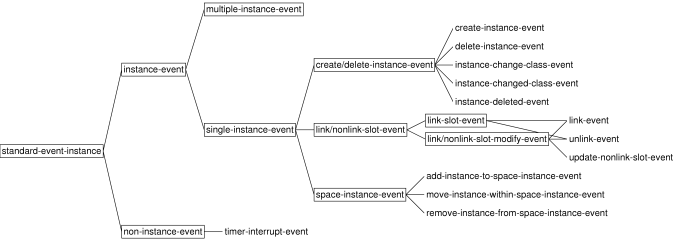
\includegraphics[scale=0.85]{gbbopen-events}
\end{center}
\W\end{iftex}

\noindent The event classes shown within rectangles are abstract classes
that cannot be signaled.

\W\xml{p}

Here are the defined event subclasses when both the \code{:gbbopen-core} and
\code{:agenda-shell} \glref{modules} have been loaded:
%
\T\begin{ifhtml}
\xml{br}
\xml{img align="center" src="agenda-shell-events.png"}
\xml{br clear="both"}
\T\end{ifhtml}
\W\begin{iftex} 
\begin{center}
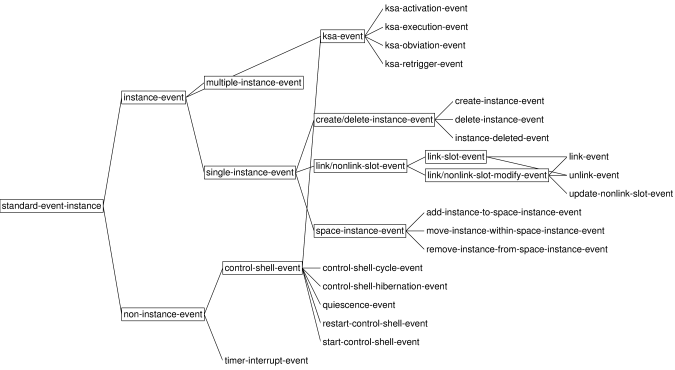
\includegraphics[scale=0.85]{agenda-shell-events}
\end{center}
\W\end{iftex}
%
The additional \code{control-shell-event} classes are defined and signaled by
the Agenda Shell.  Again classes shown within rectangles are abstract classes
that cannot be signaled.

\W\entities
\T\clearpage

%% ------------------------------------------------------------------------

\begin{functiondoc}{Function}{add-event-function}%
  {\var{function\/} [\var{event-class-specifier\/} 
    [\var{unit-class-or-instance-specifier\/}]] \\
    \code{\&key} \var{slot-names paths permanent priority\/}}
\index{event function!adding}%

%% Although the [] syntax is normally used for macros to denote optional
%% arguments, here we use them rather than &optional because of the 
%% keyword-driven argument parsing used in this function.

\fnsyntax

\fnpurpose Add an \glref{event~function} for one or more \glref{event~classes}.

\fnpackage \code{:gbbopen}

\fnmodule \code{:gbbopen-core}

\fnargs
\begin{args}{unit-class-or-instance-specifier}
\arg[function] A \glref{function~designator}
\arg[event-class-specifier] An \glref{extended~event-class~specification} 
(see below; default is \code{t})
\arg[unit-class-or-instance-specifier] An 
\glref{extended~unit-class~or~instance~specification} 
(see below; default is \code{t})
\arg[slot-names\/ \textrm{or} slot-name \T\hfil] A slot-name or list
of slot-names (default is \code{t})
\arg[paths\/ \textrm{or} path \T\hfil] A \glref{space-instance~path}
regular expression 
(default is \code{(*)})
\arg[permanent] A \glref{generalized~boolean} (default is \nil)
\arg[priority] An integer between -127 and 127, inclusive (default is \code{0})
\end{args}

\fndsyntax
\W\supp\tabletop
\eventclassspec
\subeventingspec
\syntaxsep
\unitclassinstancespec
\subclassingspec

\fndescription 
The specified \var{function\/} must accept the arguments associated with every
\glref{event~class} to which it is added.  In addition, \var{function\/}
should accept additional arguments that are associated with all
\glref{subevents} of the specified \glref{event~classes}. (This can be
achieved by specifying \code{\&allow-other-keys} in the lambda list of
\var{function}.)

The \var{paths\/} argument is either the symbol \code{t} (indicating
all \glref{space~instances}) or a list representing a regular
expression where the following reserved symbols are interpreted as
follows:
\spaceinstanceregexp

\begin{alsos}{remove-all-event-functions}
\also[remove-event-function]
\also[remove-all-event-functions]
\end{alsos}

\fnexamples
\bfindexit{evfn-printer}%
Add the event \glref{function} \entlink{evfn-printv} to the set of functions
to be invoked when \code{create-instance-event} is signaled on a
\code{hyp} \glref{unit~instance}:
%
\W\supp
\begin{example}
  (add-event-function 'evfn-printv 'create-instance-event 'hyp)
\end{example}
%
Add the event \glref{function} \entlink{evfn-printv} to the set of functions
to be invoked when \code{create-instance-event} is signaled on a
\code{hyp} \glref{unit~instance} or its subclasses:
%
\W\supp\notpretop
\begin{example}
  (add-event-function 'evfn-printv 'create-instance-event '(hyp :plus-subclasses))
\end{example}

\fnnote
\instanceevfnsnyi

\end{functiondoc}

%% ------------------------------------------------------------------------

\begin{functiondoc}{Macro}{define-event-class}{\var{event-class-name\/} 
   \code{(}\{\var{superclass-name\/}\}\superstar\code{)}
   [\var{documentation\/}] \\
   \code{(}\{\var{slot-specifier\/}\}\superstar\code{)}
   \{\var{class-option\/}\}\superstar{} 
   \returns{} \var{new-event-class\/}}
\index{event class!defining/redefining}%
\index{defining!an event class}%
\index{redefining!an event class}%

\fnsyntax

\fnpurpose Define or redefine an \glref{event~class}.

\fnpackage \code{:gbbopen}

\fnmodule \code{:gbbopen-core}

\fnargs
\begin{args}{event-class-name}
\arg[event-class-name] A non-\nil, \glref{non-keyword~symbol} that names the
\glref{event~class} 
\arg[superclass-name] A non-\nil, \glref{non-keyword~symbol} that specifies a
direct superclass of the \glref{event~class} \var{event-class-name\/}  
\arg[documentation] A documentation string
\arg[slot-specifiers] See below
\arg[class-options] See below
\arg[new-event-class] A new or modified \glref{event~class} object. 
\end{args}

\fnreturns The newly defined or modified \glref{event~class} object. 

\fndsyntax
\W\supp\tabletop
\begin{tabular}{@{~}l@{~}l}
\mbox{\var{slot-specifier\/} ::=}
 & \var{slot-name\/} \vbar{}
   \code{(}\var{slot-name\/} [[\var{slot-option\/}]]\code{)} \\
\end{tabular}
\T\\
\begin{tabular}{@{~}l@{~}l}
\mbox{\var{slot-option\/} ::=}
 & \{\code{:accessor} \var{reader-function-name\/}\}\superstar{} \vbar \\
 & \{\code{:allocation} \var{allocation-type\/}\} \vbar \\
 & \{\code{:documentation} \var{string\/}\} \vbar \\
 & \{\code{:initarg} \var{initarg-name\/}\}\superstar{} \vbar \\
 & \{\code{:initform} \var{form\/}\} \vbar \\
 & \{\code{:reader} \var{reader-function-name\/}\}\superstar{} \vbar \\
 & \{\code{:type} \var{type-specifier\/}\} \vbar{} \\
 & \{\code{:writer} \var{writer-function-name\/}\}\superstar{} \\
\end{tabular}
\T\\
\begin{tabular}{@{~}l@{~}l}
\mbox{\var{class-option\/} ::=}
 & \code{(:abstract} \var{boolean\/}\code{)} \vbar \\
 & \code{(:default-initargs .} \var{initarg-list\/}\code{)} \vbar \\
 & \code{(:documentation} \var{string\/}\code{)} \vbar \\
 & \code{(:event-metaclass} \var{event-metaclass-specifier\/}\code{)} \vbar \\
 & \code{(:event-printing} \var{event-printing-specifier\/}/code{)} \vbar \\
 & \code{(:export-class-name} \var{boolean\/}\code{)} \vbar \\
 & \code{(:export-accessors} \var{boolean\/}\code{)} \vbar \\
 & \code{(:generate-accessors} \var{direct-slots-specifier\/}\code{)} \vbar \\
 & \code{(:generate-accessors-format} 
     \{\code{:prefix} \vbar{} \code{:suffix}\} \vbar \\
 & \code{(:generate-accessors-prefix} \{\var{string\/} \vbar{}
     \var{symbol\/}\}\var\code{)} \vbar \\
 & \code{(:generate-accessors-suffix} \{\var{string\/} \vbar{}
     \var{symbol\/}\}\var\code{)} \vbar \\
 & \code{(:generate-initargs} \var{direct-slots-specifier\/}\code{)} \vbar \\
 & \code{(:metaclass} \var{class-name\/}\code{)} \\
\end{tabular}
\T\\
\begin{tabular}{@{~}l@{~}l}
\mbox{\var{event-metaclass-specifier\/} ::=}
  & non-instance-event-class \vbar{} instance-event-class \vbar{} \\
  & space-instance-event-class \vbar{} \\
  & nonlink-slot-event-class \vbar{} link-slot-event-class \\
\end{tabular}
\T\\
\begin{tabular}{@{~}l@{~}l}
\mbox{\var{direct-slots-specifier\/} ::=} & \nil{} \vbar{} \code{t} \vbar{}
  \var{included-slot-name\/}\superstar{} \vbar \\
  & \{\code{t :exclude} \var{excluded-slot-name\/}\superstar{}\} \\
\end{tabular}

\fnterms
\begin{args}{class-name}
\arg[class-name] A non-\nil, \glref{non-keyword~symbol} that names a
\glref{class} 
\arg[initarg-list] An \glref{initialization~argument~list}
\arg[slot-name] A non-\nil, \glref{non-keyword~symbol}
\end{args}

\fndescription 
\bfindexit{standard-event-class}%
Each \var{superclass-name} argument specifies a direct superclass of the new
class. If the superclass list is empty, then the direct superclass defaults to the
single class \textbf{\entlink{standard-event-instance}}.

\bfindexit{standard-event-class}%
The \code{:metaclass} \var{class-name\/} class option, if specified, must be a
subclass of \textbf{\entlinknoex{standard-event-class}}.  The default
metaclass value is the metaclass of the event superclasses of
\var{event-class-name} if they all have the same metaclass.  If the event
superclasses have multiple metaclasses, the metaclass of
\var{event-class-name} must be provided. The following table lists the
compatible event-superclass metaclasses for each \glref{event~metaclass}:

\begin{center}
\begin{tabular}{@{}l@{}l@{}c@{}l@{}c@{}l@{}c@{}l@{}c@{}l@{}c@{}}
& & \multicolumn{9}{c}{\textbf{Compatible Event-Superclass Metaclasses}}\\[4pt]
\multicolumn{1}{c}{\textbf{Event}}&~~~~~~&\code{non-}&~~&&~~&\code{space-}&~~& 
  \code{nonlink-}&~~&\code{link-}\\
\multicolumn{1}{c}{\textbf{Metaclass}}&&\code{instance}&&\code{instance}&&
   \code{instance}&&\code{slot}&&\code{slot}\\[4pt]
\code{non-instance-event-class}
   &&\textbf{X}&&          &&          &&          &&          \\
\code{instance-event-class}
   &&\textbf{X}&&\textbf{X}&&          &&          &&          \\
\code{space-instance-event-class}
   &&\textbf{X}&&\textbf{X}&&\textbf{X}&&          &&          \\
\code{nonlink-slot-event-class}
   &&\textbf{X}&&\textbf{X}&&          &&\textbf{X}&&          \\
\code{link-slot-event-class}
   &&\textbf{X}&&\textbf{X}&&          &&          &&\textbf{X}\\
\end{tabular}
\end{center}

The table in the documentation for \textbf{signal-event}
lists the \glref{initialization~arguments} that are required when
signaling an event.  These required \glref{initialization~arguments}
are based on the \glref{event~metaclass} of the \glref{event~class} of
the \glref{event} that is being signaled.

\begin{alsos}{with-generate-accessors-format}
\also[signal-event]
\also[standard-event-class]
\also[standard-event-instance]
\also[with-generate-accessors-format]
\end{alsos}

\bfindexit{non-instance-event}%
\fnexample
%
\W\supp
\begin{example}
> (define-event-class my-event (non-instance-event)
    ((my-event-arg1 :initform nil)
     (my-event-arg2 :initform nil)))
#<non-instance-event-class my-event>
\end{example}

\end{functiondoc}

%% ------------------------------------------------------------------------

\begin{functiondoc}{Function}{describe-event-printing}%
  {[\var{event-class-specifier\/} 
    [\var{unit-class-or-instance-specifier\/}]] \\
    \code{\&key} \var{slot-names paths\/}}
\index{event printing!printing information about}%
\index{printing!information about!event printing}%

%% Although the [] syntax is normally used for macros to denote optional
%% arguments, here we use them rather than &optional because of the 
%% keyword-driven argument parsing used in this function.

\fnsyntax

\fnpurpose Describe the printing of events for one or more
\glref{event~classes}. 

\fnpackage \code{:gbbopen}

\fnmodule \code{:gbbopen-core}

\fnargs
\begin{args}{unit-class-or-instance-specifier}
\arg[event-class-specifier] An \glref{extended~event-class~specification} 
(see below; default is \code{t})
\arg[unit-class-or-instance-specifier] An 
\glref{extended~unit-class~or~instance~specification} 
(see below; default is \code{t})
\arg[slot-names\/ \textrm{or} slot-name \T\hfil] A slot-name or list of
slot-names (default is \code{t})
\arg[paths\/ \textrm{or} path \T\hfil] A \glref{space-instance~path} regular
expression (default is \code{(*)})
\end{args}

\fndsyntax
\W\supp\tabletop
\eventclassspec
\subeventingspec
\syntaxsep
\unitclassinstancespec
\subclassingspec

\fndescription 
\bfindexit{*standard-output*}%
The \var{paths\/} argument is either the symbol \code{t} (indicating
all \glref{space~instances}) or a list representing a regular
expression where the following reserved symbols are interpreted as
follows:
\spaceinstanceregexp
The description is printed to the {\bf *standard-output*} stream.

\begin{alsos}{suspend-event-printing}
\also[disable-event-printing]
\also[enable-event-printing]
\also[resume-event-printing]
\also[suspend-event-printing]
\end{alsos}

\fnexample
Describe all event printing:
%
\W\supp
\begin{example}
> (describe-event-printing 'instance-event)
instance-event
  standard-unit-instance
  uc-2 [suspended]
  uc-1 [suspended]
  ksa
  ks
  root-space-instance
  standard-space-instance
\end{example}

\fnnote
\instanceevfnsnyi

\end{functiondoc}

%% ------------------------------------------------------------------------

\begin{functiondoc}{Function}{disable-event-printing}%
  {[\var{event-class-specifier\/} 
    [\var{unit-class-or-instance-specifier\/}]] \\
    \code{\&key} \var{slot-names paths\/}}
\index{event printing!disabling}%
\index{disabling!event printing}%

%% Although the [] syntax is normally used for macros to denote optional
%% arguments, here we use them rather than &optional because of the 
%% keyword-driven argument parsing used in this function.

\fnsyntax

\fnpurpose Disable the printing of events for one or more
\glref{event~classes}. 

\fnpackage \code{:gbbopen}

\fnmodule \code{:gbbopen-core}

\fnargs
\begin{args}{unit-class-or-instance-specifier}
\arg[event-class-specifier] An \glref{extended~event-class~specification} 
(see below; default is \code{t})
\arg[unit-class-or-instance-specifier] An 
\glref{extended~unit-class~or~instance~specification} 
(see below; default is \code{t})
\arg[slot-names\/ \textrm{or} slot-name \T\hfil] A slot-name or list of slot-names
(default is \code{t})
\arg[paths\/ \textrm{or} path \T\hfil] A \glref{space-instance~path} regular expression
(default is \code{(*)})
\end{args}

\fndsyntax
\W\supp\tabletop
\eventclassspec
\subeventingspec
\syntaxsep
\unitclassinstancespec
\subclassingspec

\fndescription 
The \var{paths\/} argument is either the symbol \code{t} (indicating
all \glref{space~instances}) or a list representing a regular
expression where the following reserved symbols are interpreted as
follows:
\spaceinstanceregexp

\begin{alsos}{describe-event-printing}
\also[describe-event-printing]
\also[enable-event-printing]
\also[resume-event-printing]
\also[suspend-event-printing]
\end{alsos}

\fnexample
Disable all event printing:
%
\W\supp
\begin{example}
  (disable-event-printing)
\end{example}

\fnnote
\instanceevfnsnyi

\end{functiondoc}

%% ------------------------------------------------------------------------

\begin{functiondoc}{Function}{enable-event-printing}%
{[\var{event-class-specifier\/} 
[\var{unit-class-or-instance-specifier\/}]] \\
\code{\&key} \var{slot-names paths\/}}
\index{event printing!enabling}%

%% Although the [] syntax is normally used for macros to denote optional
%% arguments, here we use them rather than &optional because of the 
%% keyword-driven argument parsing used in this function.

\fnsyntax

\fnpurpose Enable the printing of events for one or more \glref{event~classes}.

\fnpackage \code{:gbbopen}

\fnmodule \code{:gbbopen-core}

\fnargs
\begin{args}{unit-class-or-instance-specifier}
\arg[event-class-specifier] An \glref{extended~event-class~specification} 
(see below; default is \code{t})
\arg[unit-class-or-instance-specifier] An 
\glref{extended~unit-class~or~instance~specification} 
(see below; default is \code{t})
\arg[slot-names\/ \textrm{or} slot-name \T\hfil] A slot-name or list of slot-names
(default is \code{t})
\arg[paths\/ \textrm{or} path \T\hfil] A \glref{space-instance~path} regular expression
(default is \code{(*)})
\end{args}

\fndsyntax
\W\supp\tabletop
\eventclassspec
\subeventingspec
\syntaxsep
\unitclassinstancespec
\subclassingspec

\fndescription 
The \var{paths\/} argument is either the symbol \code{t} (indicating
all \glref{space~instances}) or a list representing a regular
expression where the following reserved symbols are interpreted as
follows:
\spaceinstanceregexp

\begin{alsos}{describe-event-printing}
\also[describe-event-printing]
\also[disable-event-printing]
\also[resume-event-printing]
\also[suspend-event-printing]
\end{alsos}

\fnexample
Enable event printing on all \glref{space-instance} events of
\code{hyp} \glref{unit~instances}:
%
\W\supp
\begin{example}
  (enable-event-printing '(space-instance-event :plus-subevents)
                         '(hyp :plus-subclasses))
\end{example}

\fnnote
\instanceevfnsnyi

\end{functiondoc}

%% ------------------------------------------------------------------------

\begin{functiondoc}{Function}{evfn-printv}{\var{event-class\/} 
    \&rest \var{args\/}}
\index{debugging, using evfn-printv@using \textbf{evfn-printv}}% 

\fnsyntax

\fnpurpose Assist debugging by printing forms and the results of
evaluating them to \code{*trace-output*}.

\fnpackage \code{:gbbopen}

\fnmodule \code{:gbbopen-core}

\fnargs
\begin{args}{results}
\arg[forms] An implicit \textbf{progn} of \glref{forms} to be
evaluated and printed  
\end{args}

\fnreturns The values returned by evaluating the last \var{form}.

\fndescription Evaluates \var{forms\/}, printing the \var{form\/} and the
result values of each evaluation to \code{*trace-output*}.  Any\var{form\/}
that is a string (before evaluation) is simply printed without enclosing
double-quote characters.

\fnexamples
\bfindexit{evfn-printer}%
Add the event \glref{function} \entlink{evfn-printv} to the set of functions
to be invoked when \code{create-instance-event} is signaled on a
\code{hyp} \glref{unit~instance}:
%
\W\supp
\begin{example}
  (add-event-function 'evfn-printv 'create-instance-event 'hyp)
\end{example}

\end{functiondoc}

%% ------------------------------------------------------------------------

\begin{functiondoc}{Function}{remove-all-event-functions}%
{[\var{event-class-specifier\/} 
[\var{unit-class-or-instance-specifier\/}]] \\
\code{\&key} \var{slot-names paths permanent\/}}
\index{event function!removing all}%

%% Although the [] syntax is normally used for macros to denote optional
%% arguments, here we use them rather than &optional because of the 
%% keyword-driven argument parsing used in this function.

\fnsyntax

\fnpurpose Remove all \glref{event~functions} for one or more \glref{event~classes}.

\fnpackage \code{:gbbopen}

\fnmodule \code{:gbbopen-core}

\fnargs
\begin{args}{unit-class-or-instance-specifier}
\arg[event-class-specifier] An \glref{extended~event-class~specification} 
(see below; default is \code{t})
\arg[unit-class-or-instance-specifier] An 
\glref{extended~unit-class~or~instance~specification}
(see below; default is \code{t})
\arg[slot-names\/ \textrm{or} slot-name \T\hfil] A slot-name or list of slot-names
(default is \code{t})
\arg[paths\/ \textrm{or} path \T\hfil] A \glref{space-instance~path} regular expression
(default is \code{(*)})
\arg[permanent] A \glref{generalized~boolean} (default is \nil)
\end{args}

\fndsyntax
\W\supp\tabletop
\eventclassspec
\subeventingspec
\syntaxsep
\unitclassinstancespec
\subclassingspec

\begin{alsos}{remove-event-function}
\also[add-event-function]
\also[remove-event-function]
\end{alsos}

\fnexamples
\bfindexit{evfn-printer}%
Remove all event functions associated with a
\code{create-instance-event} on a \code{hyp} \glref{unit~instance}:
%
\W\supp
\begin{example}
  (remove-all-event-functions 'create-instance-event 'hyp)
\end{example}
%
Remove all event functions associated with a
\code{create-instance-event} on a \code{hyp} \glref{unit~instance} or
its subclasses:
%
\W\supp\notpretop
\begin{example}
  (remove-all-event-functions 'create-instance-event '(hyp :plus-subclasses))
\end{example}

\fnnote
\instanceevfnsnyi

\end{functiondoc}

%% ------------------------------------------------------------------------

\begin{functiondoc}{Function}{remove-event-function}%
{\var{function\/} [\var{event-class-specifier\/} 
[\var{unit-class-or-instance-specifier\/}]] \\
\code{\&key} \var{slot-names paths permanent\/}}
\index{event function!removing}%

%% Although the [] syntax is normally used for macros to denote optional
%% arguments, here we use them rather than &optional because of the 
%% keyword-driven argument parsing used in this function.

\fnsyntax

\fnpurpose Remove an \glref{event~function} for one or more \glref{event~classes}.

\fnpackage \code{:gbbopen}

\fnmodule \code{:gbbopen-core}

\fnargs
\begin{args}{space-instance}
\arg[function] A \glref{function~designator}
\arg[event-class-specifier] An \glref{extended~event-class~specification} 
(see below; default is \code{t})
\arg[unit-class-or-instance-specifier] An 
\glref{extended~unit-class~or~instance~specification}
(see below; default is \code{t})
\arg[slot-names\/ \textrm{or} slot-name \T\hfil] A slot-name or list of slot-names
(default is \code{t})
\arg[paths\/ \textrm{or} path \T\hfil] A \glref{space-instance~path} regular expression
(default is \code{(*)})
\arg[permanent] A \glref{generalized~boolean} (default is \nil)
\end{args}

\fndsyntax
\W\supp\tabletop
\eventclassspec
\subeventingspec
\syntaxsep
\unitclassinstancespec
\subclassingspec

\begin{alsos}{remove-all-event-functions}
\also[add-event-function]
\also[remove-all-event-functions]
\end{alsos}

\fnexamples
\bfindexit{evfn-printer}%
Remove the event \glref{function} \entlink{evfn-printv} from the set of functions
to be invoked when \code{create-instance-event} is signaled on a
\code{hyp} \glref{unit~instance}:
%
\W\supp
\begin{example}
  (remove-event-function 'evfn-printv 'create-instance-event 'hyp)
\end{example}
%
Remove the event \glref{function} \entlink{evfn-printv} from the set of
functions to be invoked when \code{create-instance-event} is signaled on a
\code{hyp} \glref{unit~instance} or its subclasses:
%
\W\supp\notpretop
\begin{example}
  (remove-event-function 'evfn-printv 'create-instance-event '(hyp :plus-subclasses))
\end{example}

\fnnote
\instanceevfnsnyi

\end{functiondoc}

%% ------------------------------------------------------------------------

\begin{functiondoc}{Function}{resume-event-printing}%
{[\var{event-class-specifier\/} 
[\var{unit-class-or-instance-specifier\/}]] \\
\code{\&key} \var{slot-names paths\/}}
\index{event printing!resuming}%

%% Although the [] syntax is normally used for macros to denote optional
%% arguments, here we use them rather than &optional because of the 
%% keyword-driven argument parsing used in this function.

\fnsyntax

\fnpurpose Resume the printing of printing-enabled events for one or more
\glref{event~classes}. 

\fnpackage \code{:gbbopen}

\fnmodule \code{:gbbopen-core}

\fnargs
\begin{args}{unit-class-or-instance-specifier}
\arg[event-class-specifier] An \glref{extended~event-class~specification} 
(see below; default is \code{t})
\arg[unit-class-or-instance-specifier] An 
\glref{extended~unit-class~or~instance~specification} 
(see below; default is \code{t})
\arg[slot-names\/ \textrm{or} slot-name \T\hfil] A slot-name or list of slot-names
(default is \code{t})
\arg[paths\/ \textrm{or} path \T\hfil] A \glref{space-instance~path} regular expression
(default is \code{(*)})
\end{args}

\fndsyntax
\W\supp\tabletop
\eventclassspec
\subeventingspec
\syntaxsep
\unitclassinstancespec
\subclassingspec

\fndescription 
The \var{paths\/} argument is either the symbol \code{t} (indicating
all \glref{space~instances}) or a list representing a regular
expression where the following reserved symbols are interpreted as
follows:
\spaceinstanceregexp

\begin{alsos}{describe-event-printing}
\also[describe-event-printing]
\also[disable-event-printing]
\also[enable-event-printing]
\also[suspend-event-printing]
\end{alsos}

\fnexample
Resume all suspended event printing:
%
\W\supp
\begin{example}
  (resume-event-printing)
\end{example}

\fnnote
Resuming event printing does not enable event printing that is disabled.

\instanceevfnsnyi

\end{functiondoc}

%% ------------------------------------------------------------------------

\begin{functiondoc}{Function}{signal-event}{\var{event-class\/}
  \code{\&rest} \var{initargs\/}}
\index{event!signaling}%
\index{signaling!an event}%

\fnsyntax

\fnpurpose Signal an event

\fnpackage \code{:gbbopen}

\fnmodule \code{:gbbopen-core}

\fnargs
\begin{args}{initargs}
\arg[event-class] An \glref{event~class} or a non-\nil, \glref{non-keyword~symbol} that 
names an \glref{event~class} 
\arg[initargs] An \glref{initialization~argument~list}
\end{args}

\fndescription

\index{event function!required arguments}%
\index{function!event!required arguments}%
The following table lists the \glref{initialization~arguments} that
are required for specific event metaclasses:
\begin{center}
  \begin{tabular}{@{}l@{}l@{}}
  \textbf{Event metaclass} & \textbf{Required initargs} \\ \hline
  \code{non-instance-event-class} 
  & None \\
  \code{instance-event-class} 
  & \code{:instance} \var{unit-instance\/} \\
  \code{space-instance-event-class}~~~~~
  & \code{:instance} \var{unit-instance\/} \\
  & \code{:space-instance} \var{space-instance\/} \\ 
  \code{nonlink-slot-event-class}
  & \code{:instance} \var{unit-instance\/} \\
  & \code{:slot} \var{effective-nonlink-slot-definition\/} \\
  \code{link-slot-event-class}
  & \code{:instance} \var{unit-instance\/} \\
  & \code{:slot} \var{effective-link-definition\/} \\ \hline
\end{tabular}
\end{center}

\begin{alsos}{with-events-disabled}
\also[define-event-class]
\also[with-events-disabled]
\also[with-events-enabled]
\end{alsos}

\fnexample
%
\W\supp
\begin{example}
  (signal-event 'my-event :my-event-arg1 3)
\end{example}
\end{functiondoc}

%% ------------------------------------------------------------------------

\begin{functiondoc}{Class}{standard-event-class}{}
\index{class!standard-event-class@\textbf{standard-event-class}}%

\fnsyntax

\fnpackage \code{:gbbopen}

\fnmodule \code{:gbbopen-core}

\fndescription 
\bfindexit{define-event-class}%
The class \textbf{standard-event-class} is the superclass of classes defined
by \textbf{\entlinknoex{define-event-class}}.  It is a subclass of
\code{standard-class}.

\begin{alsos}{standard-event-instance}
\also[define-event-class]
\also[standard-event-instance]
\end{alsos}

\end{functiondoc}

%% ------------------------------------------------------------------------

\begin{functiondoc}{Event~Class}{standard-event-instance}{}
\index{class!standard-event-instance@\textbf{standard-event-instance}}%
\index{event class!standard-event-instance@\textbf{standard-event-instance}}%
  
\fnsyntax

\fnpackage \code{:gbbopen}

\fnmodule \code{:gbbopen-core}

\fndescription 
\bfindexit{standard-event-class}%
The class \textbf{standard-event-instance} is an \glref{instance} of
\textbf{\entlinknoex{standard-event-class}} and is a superclass of every
\glref{event~class} that is an \glref{instance} of
\textbf{\entlinknoex{standard-event-class}} except itself.  It is a subclass
of \textbf{\glref{standard-gbbopen-instance}}.

\begin{alsos}{standard-event-class}
\also[print-instance-slots]
\also[standard-gbbopen-instance]
\also[standard-event-class]
\end{alsos}

\end{functiondoc}

%% ------------------------------------------------------------------------

\begin{functiondoc}{Function}{suspend-event-printing}%
{[\var{event-class-specifier\/} 
[\var{unit-class-or-instance-specifier\/}]] \\
\code{\&key} \var{slot-names paths\/}}
\index{event printing!suspending}%

%% Although the [] syntax is normally used for macros to denote optional
%% arguments, here we use them rather than &optional because of the 
%% keyword-driven argument parsing used in this function.

\fnsyntax

\fnpurpose Suspend the printing of printing-enabled events for one or more
\glref{event~classes}. 

\fnpackage \code{:gbbopen}

\fnmodule \code{:gbbopen-core}

\fnargs
\begin{args}{unit-class-or-instance-specifier}
\arg[event-class-specifier] An \glref{extended~event-class~specification} 
(see below; default is \code{t})
\arg[unit-class-or-instance-specifier] An 
\glref{extended~unit-class~or~instance~specification} 
(see below; default is \code{t})
\arg[slot-names\/ \textrm{or} slot-name \T\hfil] A slot-name or list of slot-names
(default is \code{t})
\arg[paths\/ \textrm{or} path \T\hfil] A \glref{space-instance~path} regular expression
(default is \code{(*)})
\end{args}

\fndsyntax
\W\supp\tabletop
\eventclassspec
\subeventingspec
\syntaxsep
\unitclassinstancespec
\subclassingspec

\fndescription 
Suspending event printing is a convenient way of switching off event
printing without losing event-printing enabled/disabled settings.
Disabled event printing remains disabled if event printing is
resumed (by using \textbf{\entlinknoex{resume-event-printing}}).

The \var{paths\/} argument is either the symbol \code{t} (indicating
all \glref{space~instances}) or a list representing a regular
expression where the following reserved symbols are interpreted as
follows:
\spaceinstanceregexp

\begin{alsos}{describe-event-printing}
\also[describe-event-printing]
\also[disable-event-printing]
\also[enable-event-printing]
\also[resume-event-printing]
\end{alsos}

\fnexample
Suspend all event printing associated with \code{possible-hyp}
\glref{unit~instances}: 
%
\W\supp
\begin{example}
  (suspend-event-printing 't 'possible-hyp)
\end{example}

\fnnote
\instanceevfnsnyi

\end{functiondoc}

%% ------------------------------------------------------------------------

\begin{functiondoc}{Macro}{with-events-disabled}%
  {\code{(}\var{option\/}\superstar{}\code{)}
    \var{declaration\/}\superstar{}
    \var{form\/}\superstar{}
    \returns{} \var{result\/}\superstar}
\index{disabling!event signaling}%
\index{events!disabling signaling of}%
  
\fnsyntax

\fnpurpose Disable event signaling during evaluation of \var{forms}.

\fnpackage \code{:gbbopen}

\fnmodule \code{:gbbopen-core}

\fnargs
\begin{args}{options}
\arg[option] No options are currently supported
\arg[declaration] A declare expression
\arg[forms] An implicit \textbf{progn} of \glref{forms} to be evaluated
\arg[results] The values returned by evaluating the last \var{form}
\end{args}

\fnreturns The values returned by evaluating the last \var{form}.

\begin{alsos}{with-events-enabled}
\also[signal-event]
\also[with-events-enabled]
\end{alsos}

\fnexample
\bfindexit{make-instance}%
Create a \code{hyp} without signaling any events:
%
\W\supp
\begin{example}
> (with-events-disabled ()
     (\entlink{make-instance} 'hyp 
        :location (list x y)
        :classification '(:car :truck)
        :color ':red
        :belief .85
        :velocity-range '(5 35)
        :supporting-hyps supporting-hyps))
#<hyp 419 (1835 4791) 0.85 [5..35]>
\end{example}

\end{functiondoc}

%% ------------------------------------------------------------------------

\begin{functiondoc}{Macro}{with-events-enabled}%
  {\code{(}\var{option\/}\superstar{}\code{)}
    \var{declaration\/}\superstar{}
    \var{form\/}\superstar{}
    \returns{} \var{result\/}\superstar}
\index{enabling event signaling}%
\index{events!enabling signaling of}%
  
\fnsyntax

\fnpurpose Restore event signaling during evaluation of \var{forms}.

\fnpackage \code{:gbbopen}

\fnmodule \code{:gbbopen-core}

\fnargs
\begin{args}{options}
\arg[option] No options are currently supported
\arg[declaration] A declare expression
\arg[forms] An implicit \textbf{progn} of \glref{forms} to be evaluated
\arg[results] The values returned by evaluating the last \var{form}
\end{args}

\fnreturns The values returned by evaluating the last \var{form}.

\begin{alsos}{with-events-disabled}
\also[signal-event]
\also[with-events-disabled]
\end{alsos}

\fnexample
\bfindexit{make-instance}%
Create a \code{hyp} without signaling any events, then add
supporting-hypothesis links with events enabled:
%
\W\supp
\begin{example}
> (\entlink{with-events-disabled}
     (let ((hyp (\entlink{make-instance} 'hyp 
                   :location (list x y)
                   :classification '(:car :truck)
                   :color ':red
                   :belief .85
                   :velocity-range '(5 35))))
        (with-events-enabled ()
           (linkf (supporting-hyps-of hyp) supporting-hyps))
        hyp))
#<hyp 419 (1835 4791) 0.85 [5..35]>
\end{example}

\end{functiondoc}

%% ------------------------------------------------------------------------

\T\markright{}%
\T\pagestyle{plain}
\T\clearpage
\W\xname{ref-interval-entities}
\T\pagestyle{fancy}
\T\thispagestyle{fancybottom}
\T\global\def\fnlastname{ }%

\subsection{Intervals}
\label{sec:interval}%

This section contains \code{:gbbopen-core} entities that pertain to
\glref{intervals}. An interval $[a,b]$ is the set of real numbers between the
start value of the interval, $a$, and the end value, $b$, inclusive. The
interval $[x,x]$ represents the single point $x$.

An interval is represented as either a \glref{cons}, a two-element list, or a
two-element array containing the start and end values of the interval.  So, a
representation for the interval $[0,100]$ can be created as any of the
following:
\begin{tightitemize}
\item \code{(cons 0 100)}
\item \code{(list 0 100)}
\item \code{(vector 0 100)}
\end{tightitemize}
%
The function \textbf{\entlink{make-interval}} is provided for stylistic
clarity in creating an interval.

\bfindexit{make-interval}%
%
Intervals also include the unbounded intervals:
\begin{tightitemize}
\item $(-\infty,\infty)$ ~ (provided as the constant 
  \textbf{\entlink{infinite-interval}})
\item $(-\infty,x]$      ~ (for example, 
   \code{(\entlink{make-interval} x infinity)})
\item $[x,\infty)$       ~ (for example, 
   \code{(\entlink{make-interval} -infinity x)})
\end{tightitemize}

It is an error for the start value of an interval to be greater than the end
value.

\W\entities
\T\clearpage

%% ------------------------------------------------------------------------

\begin{functiondoc}[coerce-contracted-interval-rationals-to-floats-var]%
  {Variable}%
  {*coerce-contracted-interval-rationals-to-floats*}{}%

\fnsyntax

\fnpurpose Control automatic coercion of non-integer rationals to floats when
an interval is contracted into a non-integral point range by
\textbf{\entlink{expand-interval}} and \textbf{\entlink{nexpand-interval}}.

\fnpackage \code{:gbbopen}

\fnmodule \code{:gbbopen-core}

\fnvaluetype A \glref{generalized~boolean}

\fninitialvalue \nil{}

\begin{alsos}{nexpand-interval}
\also[expand-interval]
\also[nexpand-interval]
\end{alsos}

\fnexamples
%
\bfindexit{expand-interval}%
%
\W\supp
\begin{example}
> (let ((*coerce-contracted-interval-rationals-to-floats* 't))
     (expand-interval '(2 . 5) -3))
(3.5 . 3.5)
> (let ((*coerce-contracted-interval-rationals-to-floats* nil))
     (expand-interval '(2 . 5) -3))
(7/2 . 7/2)
>
\end{example}

\end{functiondoc}

%% ------------------------------------------------------------------------

\begin{functiondoc}{Function}{copy-interval}%
  {\var{interval\/}
    \returns{} \var{new-interval\/}}
\index{copy, an interval}%
\index{interval!copying}%

\fnsyntax

\fnpurpose Create a new \glref{interval} by copying \var{interval}.

\fnpackage \code{:gbbopen}

\fnmodule \code{:gbbopen-core}

\fnargs
\begin{args}{new-interval}
\arg[interval] An \glref{interval}
\arg[new-interval] An \glref{interval}
\end{args}

\fnreturns The new \glref{interval}.

\fndescription The structure of the original \var{interval\/} (\glref{cons},
two-element list, or two-element array) is maintained in the newly allocated
\var{new-interval}.

\begin{alsos}{infinite-interval}
\also[expand-interval]
\also[infinite-interval]
\also[interval-start]
\also[interval-end]
\also[make-interval]
\also[nexpand-interval]
\also[nshift-interval]
\also[shift-interval]
\end{alsos}

\fnexamples
%
\W\supp
\begin{example}
> (copy-interval '(2 5))
(2 5)
> (copy-interval '(2 . 5))
(2 . 5)
> (expand-interval #(2 5))
#(2 5)
\end{example}

\end{functiondoc}

%% ------------------------------------------------------------------------

\begin{functiondoc}{Function}{expand-interval}%
  {\var{interval amount\/}
    \returns{} \var{new-interval\/}}
\index{expand, an interval}%
\index{interval!expanding}%

\fnsyntax

\fnpurpose Create a new \glref{interval} by expanding \var{interval\/} by
\var{amount}.

\fnpackage \code{:gbbopen}

\fnmodule \code{:gbbopen-core}

\fnargs
\begin{args}{new-interval}
\arg[interval] An \glref{interval}
\arg[amount] A numbe
\arg[new-interval] An \glref{interval}
\end{args}

\fnreturns A new, expanded \glref{interval}.

\fndescription The structure of the original \var{interval\/}
(\glref{cons}, two-element list, or two-element array) is maintained in the
newly allocated, expanded \var{new-interval}.

An interval that is contracted (expanded negatively) by an amount greater than
one-half of its width will result in a zero-width \var{new-interval\/} at the
center point of the original \var{interval}.

\begin{alsos}{*coerce-contracted-interval-rationals-to-floats*}
\also[*coerce-contracted-interval-rationals-to-floats*]
\also[copy-interval]
\also[infinite-interval]
\also[interval-start]
\also[interval-end]
\also[interval-values]
\also[make-interval]
\also[nexpand-interval]
\also[nshift-interval]
\also[shift-interval]
\end{alsos}

\fnexamples
%
\W\supp
\begin{example}
> (expand-interval '(2 5) 2)
(0 7)
> (expand-interval '(2 . 5) -1)
(3 . 4)\goodpagebreak
> (expand-interval #(2 5) .5)
#(1.5 5.5)
> (expand-interval '(2 . 5) -3)
(3.5 . 3.5)
\end{example}

\end{functiondoc}

%% ------------------------------------------------------------------------

\begin{functiondoc}{Function}{expand-point}%
  {\var{point amount\/}
    \code{\&optional} \var{type-specifier\/} 
    \returns{} \var{new-interval\/}}
\index{expand, a point into an interval}%
\index{point!expanding into an interval}%

\fnsyntax

\fnpurpose Create a new \glref{interval} by expanding \var{point\/} by
\var{amount}.

\fnpackage \code{:gbbopen}

\fnmodule \code{:gbbopen-core}

\fnargs
\begin{args}{type-specifier}
\arg[point] A number
\arg[amount] A number
\arg[type-specifier] One of: \code{cons}, \code{list}, or \code{array}.
  (Default is \code{cons}.)
\arg[new-interval] An \glref{interval}
\end{args}

\fnreturns The new \glref{interval}.

\begin{alsos}{nexpand-interval}
\also[expand-interval]
\also[interval-start]
\also[interval-end]
\also[interval-values]
\also[make-interval]
\also[nexpand-interval]
\also[nshift-interval]
\also[shift-interval]
\end{alsos}

\fnexamples
%
\W\supp
\begin{example}
> (expand-point 3 2)
(1 . 5)
> (expand-point 3 2 'cons)
(1 . 5)
> (expand-point 3 2 'list)
(1 5)
> (expand-point 3 2 'array)
#(1 5)
\end{example}

\fnnote
%
\bfindex{expand-point\&}%
\bfindex{expand-point\$\&}%
\bfindex{expand-point\$}%
\bfindex{expand-point\$\$}%
\bfindex{expand-point\$\$\$}%
%
\reflink{Declared numeric}{sec:declared-numerics} versions of
\textbf{expand-point} are also provided: \textbf{expand-point\&},
\textbf{expand-point\$\&}, \textbf{expand-point\$},
\textbf{expand-point\$\$}, and \textbf{expand-point\$\$\$}.

\end{functiondoc}

%% ------------------------------------------------------------------------

\begin{functiondoc}{Constant}{infinite-interval}{}%

\fnsyntax

\fnpurpose An interval (represented as a cons) from \code{-infinity} to
\code{infinity}.

\fnpackage \code{:gbbopen}

\fnmodule \code{:gbbopen-core}

\begin{alsos}{nexpand-interval}
\also[copy-interval]
\also[expand-interval]
\also[interval-end]
\also[interval-start]
\also[interval-values]
\also[make-interval]
\also[nexpand-interval]
\also[nshift-interval]
\also[shift-interval]
\end{alsos}

\fnexample
%
\bfindexit{define-unit-class}%
\bfindexit{copy-interval}%
%
Define a \glref{unit~class}, \code{temporal-duration-mixin}, that contains a
\code{temporal-duration} slot and \glref{dimension~value} declaration:
%
\W\supp
\begin{example}
> (define-unit-class temporal-duration-mixin ()
    ((temporal-duration 
       ;; Copy the interval to allow destructive changes by
       ;; GBBopen's interval operators:
       :initform (copy-interval infinite-interval)))
    (:dimensional-values
     (temporal-duration :interval temporal-duration)))
#<standard-unit-class temporal-duration-mixin>
\end{example}

\end{functiondoc}

%% ------------------------------------------------------------------------

\begin{functiondoc}{Function}{interval-end}%
  {\var{interval\/}
    \returns{} \var{end-value\/}}
\index{end value, of an interval}%
\index{interval!obtaining the end value}%

\fnsyntax

\fnpurpose Obtain the end value of an \glref{interval}.

\fnsetf
\fnsetfsyntax{interval-end}{\var{interval\/}}{\var{end-value\/}}

\fnpackage \code{:gbbopen}

\fnmodule \code{:gbbopen-core}

\fnargs
\begin{args}{interval}
\arg[interval] An \glref{interval}
\arg[end-value] A number
\end{args}

\fnreturns The end value of the \glref{interval}.

\begin{alsos}{interval-values}
\also[interval-start]
\also[interval-values]
\end{alsos}

\fnexamples
%
\bfindexit{make-interval}
%
\W\supp
\begin{example}
> (interval-end '(1 2))
2
> (interval-end '(1 . 2))
2
> (interval-end #(1  2))
2\goodpagebreak
> (defparameter *x* (\entlink{make-interval} 1 2))
(1 . 2)
> (setf (interval-end *x*) 4)
4
> *x*
(1 . 4)
\end{example}

\end{functiondoc}

%% ------------------------------------------------------------------------

\begin{functiondoc}{Function}{interval-start}%
  {\var{interval\/} 
    \returns{} \var{start-value\/}}
\index{start value, of an interval}%
\index{interval!obtaining the start value}%

\fnsyntax

\fnpurpose Obtain the start value of an \glref{interval}.

\fnsetf
\fnsetfsyntax{interval-start}{\var{interval\/}}{\var{start-value\/}}

\fnpackage \code{:gbbopen}

\fnmodule \code{:gbbopen-core}

\fnargs
\begin{args}{interval}
\arg[interval] An \glref{interval}
\arg[start-value] A number
\end{args}

\fnreturns The start value of the \glref{interval}.

\begin{alsos}{interval-values}
\also[interval-end]
\also[interval-values]
\end{alsos}

\fnexamples
%
\bfindexit{make-interval}
%
\W\supp
\begin{example}
> (interval-start '(1 2))
1
> (interval-start '(1 . 2))
1
> (interval-start #(1 2))
1\goodpagebreak
> (defparameter *x* (\entlink{make-interval} 1 2))
(1 . 2)
> (setf (interval-start *x*) -1)
-1
> *x*
(-1 . 4)

\end{example}

\end{functiondoc}

%% ------------------------------------------------------------------------

\begin{functiondoc}{Function}{interval-values}%
  {\var{interval\/} 
    \returns{} \var{start-value, end-value\/}}
\index{start value, of an interval}%
\index{end value, of an interval}%
\index{values, start and end, of an interval}%
\index{interval!obtaining the start value}%
\index{interval!obtaining the end value}%
\index{interval!obtaining the start and end values}%

\fnsyntax

\fnpurpose Obtain the start and end values of an \glref{interval}.

\fnsetf
\fnsetfsyntax{interval-values}{\var{interval\/}}{\var{source-interval\/}}

\fnpackage \code{:gbbopen}

\fnmodule \code{:gbbopen-core}

\fnargs
\begin{args}{source-interval}
\arg[interval] An \glref{interval}
\arg[source-interval] An \glref{interval}
\arg[start-value] A number
\arg[end-value] A number
\end{args}

\fnreturns Two values: the start value and the end value of the \glref{interval}.

\begin{alsos}{interval-start}
\also[interval-end]
\also[interval-start]
\end{alsos}

\fnexamples
%
\bfindexit{make-interval}
%
\W\supp
\begin{example}
> (interval-values '(1 2))
1
2
> (interval-values '(1 . 2))
1
2
> (interval-values #(1  2))
1
2\goodpagebreak
> (defparameter *x* (\entlink{make-interval} 1 2))
(1 . 2)
> (setf (interval-values *x*) #(3 4))
#(3 4)
> *x*
(3 . 4)
\end{example}

\end{functiondoc}

%% ------------------------------------------------------------------------

\begin{functiondoc}{Function}{make-interval}%
  {\var{start end\/} 
    \code{\&optional} \var{type-specifier\/} 
    \returns{} \var{new-interval\/}}
\index{make, an interval}%
\index{interval!making}%

\fnsyntax

\fnpurpose Create a new \glref{interval} of type \var{type-specifier}.

\fnpackage \code{:gbbopen}

\fnmodule \code{:gbbopen-core}

\fnargs
\begin{args}{type-specifier}
\arg[start] A number
\arg[end] A number
\arg[type-specifier] One of: \code{cons}, \code{list}, or \code{array}.
  (Default is \code{cons}.)
\arg[new-interval] An \glref{interval}
\end{args}

\fnreturns The new \glref{interval}.

\begin{alsos}{infinite-interval}
\also[copy-interval]
\also[expand-interval]
\also[expand-point]
\also[infinite-interval]
\also[interval-start]
\also[interval-end]
\also[nexpand-interval]
\also[nshift-interval]
\also[shift-interval]
\end{alsos}

\fnexamples
%
\W\supp
\begin{example}
> (make-interval 2 5)
(2 . 5)
> (make-interval 2 5 'list)
(2 5)
> (make-interval 2 5 'cons)
(2 . 5)
> (make-interval 2 5 'array)
#(2 5)
\end{example}

\end{functiondoc}

%% ------------------------------------------------------------------------

\begin{functiondoc}{Function}{nexpand-interval}%
  {\var{interval amount\/}
    \returns{} \var{interval\/}}
\index{expand, an interval}%
\index{interval!expanding}%

\fnsyntax

\fnpurpose Expand an \glref{interval} by \var{amount}.

\fnpackage \code{:gbbopen}

\fnmodule \code{:gbbopen-core}

\fnargs
\begin{args}{interval}
\arg[interval] An \glref{interval}
\arg[amount] A number
\end{args}

\fnreturns The expanded \var{interval}.

\fndescription An interval that is contracted (expanded negatively) by an
amount greater than one-half of its width will result in a zero-width
\var{interval\/} at the center point of the original \var{interval}.

\begin{alsos}{*coerce-contracted-interval-rationals-to-floats*}
\also[*coerce-contracted-interval-rationals-to-floats*]
\also[copy-interval]
\also[expand-interval]
\also[expand-point]
\also[infinite-interval]
\also[interval-start]
\also[interval-values]
\also[interval-end]
\also[make-interval]
\also[nshift-interval]
\also[shift-interval]
\end{alsos}

\fnexamples
%
\W\supp
\begin{example}
> (nexpand-interval '(2 5) 2)
(0 7)
> (nexpand-interval '(2 . 5) -1)
(3 . 4)\goodpagebreak
> (nexpand-interval #(2 5) .5)
#(1.5 5.5)
> (nexpand-interval '(2 . 5) -3)
(3.5 . 3.5)
\end{example}

\end{functiondoc}

%% ------------------------------------------------------------------------

\begin{functiondoc}{Function}{nshift-interval}%
  {\var{interval amount\/}
    \returns{} \var{interval\/}}
\index{shift, an interval}%
\index{interval!shifting}%

\fnsyntax

\fnpurpose Shift an \glref{interval} by \var{amount}.

\fnpackage \code{:gbbopen}

\fnmodule \code{:gbbopen-core}

\fnargs
\begin{args}{interval}
\arg[interval] An \glref{interval}
\arg[amount] A number
\end{args}

\fnreturns The shifted \var{interval}.

\begin{alsos}{infinite-interval}
\also[copy-interval]
\also[expand-interval]
\also[expand-point]
\also[infinite-interval]
\also[interval-end]
\also[interval-start]
\also[interval-values]
\also[make-interval]
\also[nexpand-interval]
\also[shift-interval]
\end{alsos}

\fnexamples
%
\W\supp
\begin{example}
> (nshift-interval '(2 5) 2)
(4 7)
> (nshift-interval '(2 . 5) -1)
(1 . 4)
> (nshift-interval #(2 5) .5)
#(2.5 5.5)
\end{example}

\end{functiondoc}

%% ------------------------------------------------------------------------

\begin{functiondoc}{Function}{shift-interval}%
  {\var{interval amount\/}
    \returns{} \var{new-interval\/}}
\index{shift, an interval}%
\index{interval!shifting}%

\fnsyntax

\fnpurpose Create a new \glref{interval} by shifting \var{interval\/} by
\var{amount}.

\fnpackage \code{:gbbopen}

\fnmodule \code{:gbbopen-core}

\fnargs
\begin{args}{new-interval}
\arg[interval] An \glref{interval}
\arg[amount] A number
\arg[new-interval] An \glref{interval}
\end{args}

\fnreturns A new, shifted \glref{interval}.

\fndescription The structure of the original \var{interval\/}
(\glref{cons}, two-element list, or two-element array) is maintained in the
newly allocated, shifted \var{new-interval}.

\begin{alsos}{infinite-interval}
\also[copy-interval]
\also[expand-interval]
\also[expand-point]
\also[infinite-interval]
\also[interval-end]
\also[interval-start]
\also[interval-values]
\also[make-interval]
\also[nexpand-interval]
\also[nshift-interval]
\end{alsos}

\fnexamples
%
\W\supp
\begin{example}
> (shift-interval '(2 5) 2)
(4 7)
> (shift-interval '(2 . 5) -1)
(1 . 4)
> (shift-interval #(2 5) .5)
#(2.5 5.5)
\end{example}

\end{functiondoc}

%% ------------------------------------------------------------------------

\T\markright{}%
\T\pagestyle{plain}
\T\clearpage
\W\xname{ref-bb-repository-entities}
\T\pagestyle{fancy}
\T\thispagestyle{fancybottom}
\T\global\def\fnlastname{ }%

\subsection{Blackboard Repository}
\label{sec:bb-repository}%

This section contains \code{:gbbopen-core} entities that pertain to
\glref{space~instances} and the blackboard repository.

\W\entities
\T\clearpage

%% ------------------------------------------------------------------------

\begin{functiondoc}{Generic~Function}{add-instance-to-space-instance}%
  {\var{unit-instance space-instance-or-path\/}
    \returns{} \var{unit-instance\/}}
\index{unit instance!adding to a space instance}%
\index{space instance!adding unit instance to}%

\fnsyntax

\fnpurpose Add a \glref{unit~instance} to a \glref{space~instance}.

\fnmethods
\fnalternate{add-instance-to-space-instance}%
  {\code{(}\var{unit-instance\/} \code{standard-unit-instance)%
         (}\var{space-instance-path\/} \code{cons)}%
       \returns{} \var{unit-instance\/}}
\fnalternate{add-instance-to-space-instance}%
  {\code{(}\var{unit-instance\/} \code{standard-unit-instance)%
         (}\var{space-instance\/} \code{standard-space-instance)}%
       \returns{} \var{unit-instance\/}}

\fnpackage \code{:gbbopen}

\fnmodule \code{:gbbopen-core}

\fnargs
\begin{args}{space-instance}
\arg[unit-instance] The \glref{unit~instance} to be added
\arg[space-instance-or-path] The \glref{space~instance} or 
  \glref{space-instance~path} to which the \glref{unit~instance} is to be added
\end{args}

\fnreturns The supplied \var{unit-instance}

\fnevents
\index{events!generated by!add-instance-to-space-instance@\textbf{add-instance-to-space-instance}}%
%
\codeindexit{add-instance-to-space-instance-event}%
%
\index{events!add-instance-to-space-instance-event@\code{add-instance-to-space-instance-event}|itidx}%
%
An \code{add-instance-to-space-instance-event} is signaled.

\begin{alsos}{remove-instance-from-space-instance}
\also[define-unit-class]
\also[make-instance]
\also[make-space-instance]
\also[remove-instance-from-space-instance]
\end{alsos}

\fnexamples
\bfindexit{find-space-instance-by-path}%
Add a highly plausible hypothesis \glref{unit~instance},
\code{good-hyp}, to the \code{hyps} \glref{space~instance}:
%
\W\supp
\begin{example}
> (add-instance-to-space-instance 
    good-hyp (\entlink{find-space-instance-by-path} '(bb hyps)))
#<hyp 419 (1835 4791) 0.85 [5..35]>
\end{example}
%
or
%
\W\supp\notpretop
\begin{example}
> (add-instance-to-space-instance good-hyp '(bb hyps))
#<hyp 419 (1835 4791) 0.85 [5..35]>
\end{example}

\end{functiondoc}

%% ------------------------------------------------------------------------

\begin{functiondoc}{Generic~Function}{allowed-unit-classes-of}%
  {\var{space-instance\/}
    \returns{} \var{extended-unit-classes-specification-list\/}}
\index{space instance!allowed unit classes}%

\fnsyntax

\fnpurpose Return the \glref{extended~unit-classes~specifications} of
\glref{unit~classes} whose \glref{instances} are allowed on a
\glref{space~instance}.

\fnmethods
\fnalternate{allowed-unit-classes-of}%
  {\code{(}\var{space-instance\/} \code{standard-space-instance)}
    \returns{} \var{extended-unit-class-specification-list\/}}

\fnpackage \code{:gbbopen}

\fnmodule \code{:gbbopen-core}

\fnargs
\begin{args}{extended-unit-classes-specification-list}
\arg[space-instance] A \glref{space~instance}
\arg[extended-unit-classes-specification-list] A proper list
\end{args}

\fnreturns A list of \glref{extended~unit-classes~specifications}; \code{t},
if instances of any \glref{unit~class} are allowed on the
\glref{space~instance}; or \nil, if no \glref{unit~instances} are allowed on
the \glref{space~instance}

\begin{alsos}{make-space-instance}
\also[make-space-instance]
\end{alsos}

\fnexample
Return the \glref{extended~unit-classes~specifications} describing the allowed
classes that can have their \glref{unit~instances} stored on the \code{(bb
  hyps)} \glref{space~instance}:
%
\W\supp
\begin{example}
> (allowed-unit-classes-of '(bb hyps))
((hyp :plus-subclasses))
\end{example}

\end{functiondoc}

%% ------------------------------------------------------------------------

\begin{functiondoc}{Function}{change-space-instance}{%
    \var{space-instance\/}
    \code{\&key} \var{allowed-unit-classes dimensions storage\/}
    \returns{} \var{space-instance\/}}
\index{changing!a space instance characteristics}%
\index{allowed unit classes!of a space instance!changing}%
\index{dimensions!of a space instance!changing}%
\index{storage!of a space instance!changing}%
\index{space instance!changing!allowed unit classes}%
\index{space instance!changing!dimensions}%
\index{space instance!changing!storage}%
 
\fnsyntax

\fnpurpose Change the dimensions, allowed unit classes, and storage of a
\glref{space~instance}.

\fnpackage \code{:gbbopen}

\fnmodule \code{:gbbopen-core}

\fnargs
\begin{args}{allowed-unit-classes}
\arg[space-instance-or-path] The \glref{space~instance} or
  \glref{space-instance~path} to be changed
\arg[allowed-unit-classes] An \glref{extended~unit-classes~specification} 
  or \nil{} (see below; default is \code{t})
\arg[dimensions] A list of \code{(}\var{\glref{dimension-name}}
 \var{dimension-type-specifier\/}\code{)} pairs (default is \nil)  
\arg[storage] A \glref{storage~specification}
(see below; default is \mbox{\code{(t t unstructured)}} or \nil{} if
\var{allowed-unit-classes\/} is \nil) 
\arg[space-instance] The \glref{space~instance}
\end{args}

\fnreturns
The \glref{space~instance} that was changed.

\fnevents
\index{events!generated by!change-space-instance@\textbf{change-space-instance}}%
%
\codeindexit{remove-instance-from-space-instance-event}%
%
\index{events!remove-instance-from-space-instance-event@\code{remove-instance-from-space-instance-event}|itidx}%
%
When the allowed unit classes of \var{space-instance\/} are made more
restrictive, \glref{unit~instances} that are no longer allowed on the
\glref{space~instance} are removed from \var{space-instance\/}, signaling a
\code{remove-instance-from-space-instance-event} for each removed unit
instance.

\fndsyntax
\W\supp\tabletop
\begin{tabular}{@{~}l@{~}l}
\mbox{\var{allowed-unit-classes\/} ::=} \var{unit-classes-specifier\/}
  \vbar{} \nil\\
\end{tabular}
\T\\[4pt]
\begin{tabular}{@{~}l@{~}l}
\mbox{\var{dimension-type-specifier\/} ::=}
  & \code{:ordered} \vbar{} 
    \code{(:ordered} [\var{ordered-comparison-type\/}]\code{)} \vbar{} \\
  & \code{:enumerated} \vbar{}
    \code{(:enumerated} [\var{enumerated-comparison-type\/}]\code{)} \vbar{} \\
  & \code{:boolean} \vbar{}
    \code{(:boolean} [\var{boolean-comparison-type\/}]\code{)} \\
\end{tabular}
\T\\
\comparisontypespecs
\T\\[4pt]
\unitclassesspec
\syntaxsep
\storagespec
\T\\[4pt]
\comparisontypenote

\fnterms
\begin{args}{dimension-name}
\arg[dimension-name] A symbol specifying a \glref{dimension} 
\end{args}

\begin{alsos}{make-space-instance}
\also[make-space-instance]
\end{alsos}

\fnexamples
%
Change the storage of \glref{space~instance} \code{(bb hyp}) to the default
unstructured storage for all \glref{unit~instances}:
%
\W\supp
\begin{example}
> (change-space-instance '(bb hyps) :storage nil)
#<standard-space-instance (bb hyps)>
>
\end{example}
%
Now change it to store \code{hyp} \glref{unit~instances} with uniform-bucket
storage for indexing in the \code{x} and \code{y} dimensions and hashed
storage in the \code{classification} dimension:
%
\W\supp\notpretop
\begin{example}
> (change-space-instance-storage '(bb hyps)
     :storage '(((hyp :plus-subclasses) (x y) 
                  uniform-buckets :layout ((0 10000 100)
                                           (0 10000 100)))
                ((hyp :plus-subclasses) (classification) 
                  hashed)))
#<standard-space-instance (bb hyps)>
>
\end{example}
%
Now change it to store only \code{hyp} \glref{unit~instances} (no subclasses)
with uniform-bucket storage for indexing in the \code{x} and \code{y}
dimensions and hashed storage in the \code{classification} dimension:
%
\W\supp\notpretop
\begin{example}
> (change-space-instance-storage '(bb hyps)
     :allowed-unit-classes 'hyp     
     :storage '((hyp (x y) 
                 uniform-buckets :layout ((0 10000 100)
                                          (0 10000 100)))
                (hyp (classification) hashed)))
#<standard-space-instance (bb hyps)>
> 
\end{example}
%
Any \glref{unit~instances} that are subclasses of \code{hyp} are removed from
the \code{(bb hyps)} \glref{space~instance} by the above change in allowed
unit classes.

\end{functiondoc}

%% ------------------------------------------------------------------------

\begin{functiondoc}{Generic~Function}{children-of}%
  {\var{space-instance\/}
    \returns{} \var{space-instances\/}}
\index{space instance!finding children of}%

\fnsyntax

\fnpurpose Return the child space instances of a \glref{space~instance}.

\fnmethods
\fnalternate{children-of}%
  {\code{(}\var{space-instance\/} \code{root-space-instance)}
    \returns{} \var{space-instances\/}}

\fnpackage \code{:gbbopen}

\fnmodule \code{:gbbopen-core}

\fnargs
\begin{args}{space-instances}
\arg[space-instance] A \glref{space~instance}
\arg[space-instances] A proper list
\end{args}

\fnreturns A list of the child space instances.

\begin{alsos}{make-space-instance}
\also[make-space-instance]
\also[parent-of]
\end{alsos}

\fnexample
\bfindexit{find-space-instance-by-path}%
Return the child space instances  of the \code{(bb)} \glref{space~instance}:
%
\W\supp
\begin{example}
> (children-of (\entlink{find-space-instance-by-path} '(bb))
(#<standard-space-instance (bb hyps)>
 #<standard-space-instance (bb probable-hyps)>
 #<standard-space-instance (bb rejected-hyps)>)
\end{example}

\fnnote The returned list of child \glref{space~instances} should not be
destructively altered.

\end{functiondoc}

%% ------------------------------------------------------------------------

\begin{functiondoc}{Function}{clear-space-instances}%
{\var{space-instances\/}}
\index{space instance!removing all unit instances from}%

\fnsyntax

\fnpurpose Remove (but not delete) all \glref{unit~instances} from
\glref{space~instances}.

\fnpackage \code{:gbbopen}

\fnmodule \code{:gbbopen-core}

\fnargs
\begin{args}{space-instances}
\arg[space-instances] A \glref{space~instance}, a list of
  \glref{space~instances}, a \glref{space-instance~path} regular
  expression, or \code{t} (indicating all space instances)
\end{args}

\fnevents
\index{events!generated by!remove-instance-from-space-instance@\textbf{remove-instance-from-space-instance}}%
%
\codeindexit{remove-instance-from-space-instance-event}%
%
\index{events!remove-instance-from-space-instance-event@\code{remove-instance-from-space-instance-event}|itidx}%
%
A \code{remove-instance-from-space-instance-event} is signaled
for each \glref{unit~instance} that is removed from a \glref{space~instance}.

\begin{alsos}{map-instances-on-space-instances}
\also[do-instances-on-space-instances]
\also[map-instances-on-space-instances]
\end{alsos}

\fnexamples
\index{events!remove-instance-from-space-instance-event@\code{remove-instance-from-space-instance-event}|itidx}%
\bfindexit{remove-instance-from-space-instance}%
Remove all the \glref{unit~instances} that
reside on the \code{(bb probable-hyps)} \glref{space~instance}:
%
\W\supp
\begin{example}
  (clear-space-instances
    (\entlink{find-space-instance-by-path} '(bb probable-hyps)))
\end{example}
%
or
%
\W\supp\notpretop
\begin{example}
  (clear-space-instances '(bb probable-hyps))
\end{example}
%
or
%
\W\supp\notpretop
\begin{example}
  (clear-space-instances
    (\entlink{find-space-instances} '(bb probable-hyps)))
\end{example}

\end{functiondoc}

%% ------------------------------------------------------------------------

\begin{functiondoc}{Macro}{define-space-class}%
   {\var{space-class-name\/} 
   \code{(}\{\var{superclass-name\/}\}\superstar\code{)}
   [\var{documentation\/}] \\
   \code{(}\{\var{slot-specifier\/}\}\superstar\code{)}
   \{\var{class-option\/}\}\superstar{}
   \returns{} \var{new-space-class\/}}
\index{space class!defining/redefining}%
\index{defining!a space class}%
\index{redefining!a space class}%

\fnsyntax

\fnpurpose Define or redefine a \glref{space~class}.

\fnpackage \code{:gbbopen}

\fnmodule \code{:gbbopen-core}

\fnargs
\begin{args}{space-class-name}
\arg[space-class-name] A non-\nil, \glref{non-keyword~symbol} that names the
\glref{space~class} 
\arg[superclass-name] A non-\nil, \glref{non-keyword~symbol} that specifies a
direct superclass of the \glref{space~class} \var{space-class-name\/}  
\arg[documentation] A documentation string
\arg[slot-specifiers] See below
\arg[class-options] See below
\arg[new-space-class] A new or modified \glref{space~class} object
\end{args}

\fnreturns The newly defined or modified \glref{space~class} object.

\fnerrors The specified \var{superclass-names\/} do not include at least
one \glref{space~class} name.  This error is signaled on class finalization.

\fndsyntaxwgray
\W\supp\tabletop
\begin{tabular}{@{~}l@{~}l}
\mbox{\var{slot-specifier\/} ::=}
 & \var{slot-name\/} \vbar \\
 & \code{(}\var{nonlink-slot-name\/}
   [[\var{nonlink-slot-option\/}]]\code{)} \vbar \\
 & \code{(}\var{link-slot-name\/} [[\var{link-slot-option\/}]]\code{)} \\
\end{tabular}
\T\\
\begin{tabular}{@{~}l@{~}l}
\mbox{\var{nonlink-slot-name\/} ::=} & \var{slot-name}\\
\end{tabular}
\T\\
\begin{tabular}{@{~}l@{~}l}
\mbox{\var{link-slot-name\/} ::=} & \var{slot-name}\\
\end{tabular}
\T\\
\begin{tabular}{@{~}l@{~}l}
\mbox{\var{link-slot-option\/} ::=}
 & \var{slot-option\/} \vbar \\
 & \{\code{:link} \var{inverse-link-slot-specifier\/}\} \vbar \\
 & \{\code{:singular} \var{boolean\/}\} \vbar \\
 & \{\code{:sort-function} \var{function\/}\} \vbar \\
 & \{\code{:sort-key} \var{function\/}\} \\
\end{tabular}
\T\\
\begin{tabular}{@{~}l@{~}l}
\mbox{\var{inverse-link-slot-specifier\/} ::=} & 
  \code{(}\var{unit-class-name link-slot-name\/} 
    [\code{:singular} \var{boolean\/}]\code{)} \vbar{} \\
  & \code{:reflexive} \\
\end{tabular}
\T\\
\begin{tabular}{@{~}l@{~}l}
\mbox{\var{nonlink-slot-option\/} ::=}
 & \var{slot-option\/} \vbar \\
 & \{\code{:reader} \var{reader-function-name\/}\}\superstar{} \vbar \\
 & \{\code{:writer} \var{writer-function-name\/}\}\superstar{} \\
\end{tabular}
\T\\
\begin{tabular}{@{~}l@{~}l}
\mbox{\var{slot-option\/} ::=}
 & \{\code{:accessor} \var{reader-function-name\/}\}\superstar{} \vbar \\
 & \{\code{:allocation} \var{allocation-type\/}\} \vbar \\
 & \{\code{:documentation} \var{string\/}\} \vbar \\
 & \{\code{:initarg} \var{initarg-name\/}\}\superstar{} \vbar \\
 & \{\code{:initform} \var{form\/}\} \vbar \\
 & \{\code{:type} \var{type-specifier\/}\} \\
\end{tabular}
\T\\
\begin{tabular}{@{~}l@{~}l}
\mbox{\var{class-option\/} ::=}
 & \code{(:abstract} \var{boolean\/}\code{)} \vbar \\
 & \code{(:default-initargs .} \var{initarg-list\/}\code{)} \vbar \\
 & \code{(:dimensional-values} 
   \var{dimensional-value-specifier\/}\superstar\code{)} \vbar \\
 & \code{(:documentation} \var{string\/}\code{)} \vbar \\
 & \code{(:export-class-name} \var{boolean\/}\code{)} \vbar \\
 & \code{(:export-accessors} \var{boolean\/}\code{)} \vbar \\
 & \code{(:generate-accessors} \var{direct-slots-specifier\/}\code{)} \vbar \\
 & \code{(:generate-accessors-format} 
     \{\code{:prefix} \vbar{} \code{:suffix}\} \vbar \\
 & \code{(:generate-accessors-prefix} \{\var{string\/} \vbar{}
     \var{symbol\/}\}\var\code{)} \vbar \\
 & \code{(:generate-accessors-suffix} \{\var{string\/} \vbar{}
     \var{symbol\/}\}\var\code{)} \vbar \\
 & \code{(:generate-initargs} \var{direct-slots-specifier\/}\code{)} \vbar \\
 & \code{(:initial-space-instances}
     \var{initial-space-instance-specifier\/}\code{)} \vbar \\
 & \code{(:instance-name-comparison-test}
     \var{instance-name-comparison-test\/}\code{)} \vbar \\
 & \code{(:metaclass} \var{class-name\/}\code{)}  \vbar \\
 & \code{(:retain} \{\var{boolean\/} \vbar{} \code{:propagate}\}\code{)} \\
\end{tabular}
\T\\
\begin{tabular}{@{~}l@{~}l}
\mbox{\var{initial-space-instance-specifier\/} ::=}
  & \{\var{space-instance-path\/}\superplus{} \vbar{}
  \var{function\/}\} \\ 
\end{tabular}
\T\\
\dimensionalvaluesspec
\T\\
\begin{tabular}{@{~}l@{~}l}
\mbox{\var{direct-slots-specifier\/} ::=} & \nil{} \vbar{} \code{t} \vbar{}
  \var{included-slot-name\/}\superstar{} \vbar \\
  & \{\code{t :exclude} \var{excluded-slot-name\/}\superstar{}\} \\
\end{tabular}
\T\\[4pt]
\comparisontypenote
\T\\
\dimensionalspecnote

\fnterms
\begin{args}{instance-name-comparison-test}
\arg[class-name] A non-\nil, \glref{non-keyword~symbol} that names a
\glref{class} 
\arg[initarg-list] An \glref{initialization~argument~list}
\arg[slot-name] A non-\nil, \glref{non-keyword~symbol}
\arg[instance-name-comparison-test] One of the four standardized hash table
test function names: \code{eq}, \code{eql}, \code{equal}, or \code{equalp}
(default for classes of metaclass \textbf{\entlinknoex{standard-unit-class}}
is \code{eql})
\end{args}

\fndescription A \var{dimension-value-place\/} with two
\var{slot-names\/} can be specified only for \code{:interval}
dimension-value types.

\bfindexit{standard-space-class}%
Each \var{superclass-name} argument specifies a direct superclass of the new
class. If the superclass list is empty, then the direct superclass defaults to the
single class \textbf{\entlink{standard-space-instance}}.

\bfindexit{standard-space-class}%
The \code{:metaclass} \var{class-name\/} class option, if specified, must be a
subclass of \textbf{\entlinknoex{standard-space-class}}.  The default
metaclass value is \textbf{\entlinknoex{standard-space-class}}.

\fndspar{Inheritance of class options}
\classoptioninheritance

\begin{alsos}{with-generate-accessors-format}
\also[define-unit-class]
\also[delete-blackboard-repository]
\also[make-space-instance]
\also[standard-space-class]
\also[standard-space-instance]
\also[with-generate-accessors-format]
\end{alsos}

\fnexample 
\bfindexit{make-space-instance}%
Define a \glref{space~class},
\code{space-instance-with-lock}, that has an additional \glref{slot}
containing a \glref{lock} that can be used to synchronize
operations on each \glref{space~instance} of that class. Then, create
one \glref{instance} of the \code{space-instance-with-lock}
\glref{space~class}.
%
\W\supp
\begin{example}
> (define-space-class space-with-lock ()
    ((lock :initform (\entlink{make-lock} :name "Space-Instance Lock"))))
#<standard-space-class space-with-lock>
> (\entlink{make-space-instance} '(bb hyps) 
    :class 'space-with-lock)
#<space-with-lock (bb hyps)>
\end{example}

\end{functiondoc}

%% ------------------------------------------------------------------------

\begin{functiondoc}{Function}{delete-blackboard-repository}%
  {\code{\&key} \var{all-classes
                     disable-events 
                     retain-classes\/}}
\index{unit instance!deleting all}%
\index{space instance!deleting all}%

\fnsyntax

\fnpurpose Delete all \glref{unit} and \glref{space~instances}.

\fnpackage \code{:gbbopen}

\fnmodule \code{:gbbopen-core}

\fnargs
\begin{args}{disable-events}
\arg[all-classes] A \glref{generalized~boolean} (default is \nil)
\arg[disable-events] A \glref{generalized~boolean} (default is \code{t})
\arg[retain-classes] An \glref{extended~unit-classes~specification}
  (see below)
\end{args}

\fnevents
\index{events!generated by!delete-blackboard-repository@\textbf{delete-blackboard-repository}}%
%
\codeindexit{delete-instance-event}%
\codeindexit{instance-deleted-event}%
\codeindexit{remove-instance-from-space-instance-event}%
\codeindexit{unlink-event}%
%
\index{events!delete-instance-event@\code{delete-instance-event}|itidx}%
\index{events!instance-deleted-event@\code{instance-deleted-event}|itidx}%
\index{events!remove-instance-from-space-instance-event@\code{remove-instance-from-space-instance-event}|itidx}%
\index{events!unlink-event@\code{unlink-event}|itidx}%
%
If \var{disable-events} is \nil, the following events may be signaled as
\glref{unit~instances} and \glref{space~instances} are deleted:
\begin{tightitemize}
\item \code{delete-instance-event}
\item \code{unlink-event}
\item \code{remove-instance-from-space-instance-event}
\item \code{instance-deleted-event}
\end{tightitemize}

\fndsyntax
\W\supp\tabletop
\unitclassesspec

\fndescription Calling \textbf{delete-blackboard-repository} deletes all
\glref{unit~instances} and \glref{space~instances} that have not been defined
with a \code{:retain} class option (unless overridden by \var{all-classes\/}).
All \glref{unit~instances} of \glref{unit~classes} specified by
\var{retain-classes\/} are also retained.  If both \var{all-classes\/} and
\var{retain-classes\/} are specified, the classes specified
\var{retain-classes\/} are retained, but all other \glref{unit~instances} are
deleted.  The instance-name counters of all non-retained \glref{unit~classes}
are reset to their initial values.

\textbf{Delete-blackboard-repository} does not undefine any class
definitions, functions, methods, etc.

\begin{alsos}{initial-class-instance-number}
\also[delete-instance]
\also[delete-all-space-instances]
\also[delete-space-instance]
\also[initial-class-instance-number]
\end{alsos}

\fnexamples 

Delete all \glref{unit~instances} and \glref{space~instances}
(except for the \glref{unit~instances} of \glref{unit~classes} that have been
defined to be retained by default):
%
\W\supp
\begin{example}
  (delete-blackboard-repository)
\end{example}
%
As above, but also delete all \glref{unit~instances} of \glref{unit~classes}
that have been defined to be retained by default:
%
\W\supp\notpretop
\begin{example}
  (delete-blackboard-repository :all-classes t)
\end{example}

\fnnote 
\bfindexit{with-events-disabled}%
\bfindexit{with-events-enabled}%
This function and \textbf{\entlink{reset-gbbopen}} are the only GBBopen
functions that disable \glref{event} signaling by default.  This conflicts
with the normal use of \textbf{\entlinknoex{with-events-disabled}} and
\textbf{\entlinknoex{with-events-enabled}} macros for controlling
\glref{event} signaling, but having \glref{events} disabled is the desired
behavior in almost every \code{delete-blackboard-repository} situation.

\end{functiondoc}

%% ------------------------------------------------------------------------

\begin{functiondoc}{Function}{delete-all-space-instances}{\noargs}
\index{deleting!all space instances}%
\index{space instance!deleting}%

\fnsyntax

\fnpurpose Delete all \glref{space~instances}.

\fnpackage \code{:gbbopen}

\fnmodule \code{:gbbopen-core}

\fnevents \codeindexit{delete-instance-event}%
\index{events!generated by!delete-all-space-instances@\textbf{delete-all-space-instances}}%
%
\codeindexit{delete-instance-event}%
\codeindexit{instance-deleted-event}%
\codeindexit{remove-instance-from-space-instance-event}%
\codeindexit{unlink-event}%
%
\index{events!delete-instance-event@\code{delete-instance-event}|itidx}%
\index{events!instance-deleted-event@\code{instance-deleted-event}|itidx}%
\index{events!remove-instance-from-space-instance-event@\code{remove-instance-from-space-instance-event}|itidx}%
\index{events!unlink-event@\code{unlink-event}|itidx}%
%
A \code{delete-instance-event} is signaled at the start of the deletion
process of each \glref{space~instance} and an \code{instance-deleted-event} is
signaled when the deletion of each \glref{space~instance} has been completed.
The following events may also be signaled if a \var{space-instance} is,
itself, on a \glref{space~instance} or is linked to other
\glref{unit~instances}:
%
\begin{tightitemize}
\item \code{unlink-event}
\item \code{remove-instance-from-space-instance-event}
\end{tightitemize}

\begin{alsos}{delete-blackboard-repository}
\also[delete-all-space-instances]
\also[delete-blackboard-repository]
\also[delete-space-instance]
\also[make-space-instance]
\also[reset-gbbopen]
\also[reset-unit-class]
\end{alsos}

\fnexample
Delete every space instance:
%
\W\supp
\begin{example}
  (delete-all-space-instances)
\end{example}

\end{functiondoc}

%% ------------------------------------------------------------------------

\begin{functiondoc}{Generic~Function}{delete-space-instance}%
    {\var{space-instance-or-path\/}
    \returns{} \var{deleted-space-instance\/}}
\index{deleting!a space instance}%
\index{space instance!deleting}%

\fnsyntax

\fnpurpose Delete a \glref{space~instance}.

\fnmethods
\fnalternate{delete-space-instance}%
  {\code{(}\var{space-instance-path\/} \code{cons)}
    \returns{} \var{deleted-space-instance\/}}
\fnalternate{delete-space-instance}%
  {\code{(}\var{space-instance\/} \code{standard-space-instance)}
    \returns{} \var{deleted-space-instance\/}}

\fnpackage \code{:gbbopen}

\fnmodule \code{:gbbopen-core}

\fnargs
\begin{args}{space-instance-or-path}
\arg[space-instance-or-path] The \glref{space~instance} or
  \glref{space-instance~path} to be deleted
\arg[deleted-space-instance] A \glref{space~instance}
\end{args}

\fnreturns The deleted \glref{space~instance}.

\fnevents
\index{events!generated by!delete-space-instance@\textbf{delete-space-instance}}%
%
\codeindexit{delete-instance-event}%
\codeindexit{instance-deleted-event}%
\codeindexit{remove-instance-from-space-instance-event}%
\codeindexit{unlink-event}%
%
\index{events!delete-instance-event@\code{delete-instance-event}|itidx}%
\index{events!instance-deleted-event@\code{instance-deleted-event}|itidx}%
\index{events!remove-instance-from-space-instance-event@\code{remove-instance-from-space-instance-event}|itidx}%
\index{events!unlink-event@\code{unlink-event}|itidx}%
%
A \code{delete-instance-event} is signaled at the start of the
deletion process and an \code{instance-deleted-event} is
signaled when the deletion has been completed.  The following events
may also be signaled if the \var{space-instance} is, itself, on a
\glref{space~instance} or is linked to other \glref{unit~instances}:
\begin{tightitemize}
\item \code{unlink-event}
\item \code{remove-instance-from-space-instance-event}
\end{tightitemize}

\begin{alsos}{delete-blackboard-repository}
\also[delete-all-space-instances]
\also[delete-blackboard-repository]
\also[delete-instance]
\also[make-space-instance]
\also[reset-gbbopen]
\also[reset-unit-class]
\end{alsos}

\fnexamples
\bfindexit{find-space-instance-by-path}%
Delete the \code{(bb hyps)} \glref{space~instance}:
%
\W\supp
\begin{example}
> (delete-space-instance (\entlink{find-space-instance-by-path} '(bb hyps))
#<standard-space-instance (bb hyps) [Deleted]>
\end{example}
%
or simply
%
\W\supp\notpretop
\begin{example}
> (delete-space-instance '(bb hyps)
#<standard-space-instance (bb hyps) [Deleted]>
\end{example}

\end{functiondoc}

%% ------------------------------------------------------------------------

\begin{functiondoc}{Function}{describe-blackboard-repository}{\noargs}

\fnsyntax

\fnpurpose \index{space instance!printing information about}%
\index{blackboard repository!printing information about}%
\index{printing!information about!the blackboard repository}%
Print information about the \glref{unit} and \glref{space~instances} in the
blackboard repository.

\fnpackage \code{:gbbopen}

\fnmodule \code{:gbbopen-core}

\fndescription
\bfindexit{delete-blackboard-repository}%
\bfindexit{*standard-output*}%
Information is printed about the \glref{space~instances} in the blackboard
repository and their contents.  The total count of the
\glref{unit~instances} of each \glref{unit~class} (including ones that
do not reside on any \glref{space~instance}) is also printed, as well
as a character that indicates if the \glref{unit~class} has been
defined to be \textit{retained} by
\textbf{\entlink{delete-blackboard-repository}}.  A plus sign
indicates that the retention status will be propagated to subclasses
of the unit class, while an asterisk (\code{*}) indicates a retain,
But not propagated, status for the \glref{unit~class}.

The description is printed to the {\bf *standard-output*} stream.

\fnexample
%
\W\supp
\begin{example}
> (describe-blackboard-repository)

Space Instance                Contents
--------------                --------
bb                            
   hyps                       15223 Instances (hyp 1479; sensor-report 13744)
   probable-hyps              Empty
   rejected-hyps              216 Instances (hyp 216)

Unit Class                    Instances
----------                    ---------
control-shell                         1 *
hyp                                1695
ks                                   13 + 
ksa                                 891 +
ksa-queue                             2 +
ordered-ksa-queue                     1 +
sensor-report                     13744
standard-space-instance               3
                              ---------
                                  16350 instances
\end{example}

\fnnote 
%
\REPLindex{:dsbb}%
%
\textbf{Describe-blackboard-repository} can be invoked using the
\glref{REPL~command} \code{:dsbb}.

\end{functiondoc}

%% ------------------------------------------------------------------------

\begin{functiondoc}{Generic~Function}{describe-space-instance}%
  {\var{space-instance-or-path\/}}
\index{space instance!printing information about}%
\index{printing!information about!space instance}%

\fnsyntax

\fnpurpose Describe a \glref{space~instance}.

\fnmethods
\fnalternate{describe-space-instance}%
  {\code{(}\var{space-instance-path\/} \code{cons)}}
\fnalternate{describe-space-instance}%
  {\code{(}\var{space-instance\/} \code{standard-space-instance)}}

\fnpackage \code{:gbbopen}

\fnmodule \code{:gbbopen-core}

\fnargs
\begin{args}{space-instance}
\arg[space-instance-or-path] A \glref{space~instance} or a 
  \glref{space-instance~path}
\end{args}

\fndescription
\bfindexit{*standard-output*}%
The description is printed to the {\bf *standard-output*} stream.

\begin{alsos}{describe-space-instance-storage}
\also[describe-instance]
\also[describe-space-instance-storage]
\also[make-space-instance]
\end{alsos}

\fnexample
Describe the \code{hyps} \glref{space~instance}:
%
\W\supp
\begin{example}
> (describe-space-instance '(bb hyps))
  Standard-space-instance #<standard-space-instance (bb hyps)>
    Path: (bb hyps)
    Allowed unit classes:
      (hyp :plus-subclasses)
    Dimensions:
      (belief (:ordered number))
      (velocity-range (:ordered number))
      (color (:enumerated eq))
      (classification (:enumerated eq))
      (x (:ordered fixnum))
      (y (:ordered fixnum))
\end{example}

\fnnote 
%
\REPLindex{:dsi}%
%
\textbf{Describe-space-instance} can be invoked using the \glref{REPL~command}
\code{:dsi}, which also sets \code{=} to the described \glref{space~instance}.

\end{functiondoc}

%% ------------------------------------------------------------------------

\begin{functiondoc}{Generic~Function}{describe-space-instance-storage}%
  {\var{space-instance-or-path\/}}
\index{space instance!printing information about}%
\index{printing!information about!space instance}%

\fnsyntax

\fnpurpose Describe the storage structure of a \glref{space~instance}.

\fnmethods
\fnalternate{describe-space-instance-storage}%
  {\code{(}\var{space-instance-path\/} \code{cons)}}
\fnalternate{describe-space-instance-storage}%
  {\code{(}\var{space-instance\/} \code{standard-space-instance)}}

\fnpackage \code{:gbbopen}

\fnmodule \code{:gbbopen-core}

\fnargs
\begin{args}{space-instance}
\arg[space-instance-or-path] A \glref{space~instance} or a 
  \glref{space-instance~path}
\end{args}

\fndescription
\bfindexit{*standard-output*}%
The description is printed to the {\bf *standard-output*} stream.

\begin{alsos}{describe-space-instance}
\also[describe-space-instance]
\also[describe-instance]
\also[make-space-instance]
\end{alsos}

\fnexample
Describe the storage structure of the \code{hyps} \glref{space~instance}:
%
\W\supp
\begin{example}
> (describe-space-instance-storage '(bb hyps))
  Standard-space-instance #<standard-space-instance (bb hyps)>
  2d-Uniform-Buckets (hyp+) (x y) 1.4 (857/611)
     hyp             479
     sub-hyp         132
  Unstructured-Storage (t) t N/A
\end{example}

\fnnote 
%
\REPLindex{:dsis}%
%
\textbf{Describe-space-instance-storage} can be invoked using the
\glref{REPL~command} \code{:dsis}, which also sets \code{=} to the described
\glref{space~instance}.

\end{functiondoc}

%% ------------------------------------------------------------------------

\begin{functiondoc}{Macro}{do-space-instances}%
  {(\var{var space-instance-regexp\/})
    \mbox{\{\var{tag\/} \vbar{} \var{form\/}\}\superstar}}

\fnsyntax

\fnpurpose Iterate over each \glref{space~instance} that matches a
\glref{path-expression} pattern.

\fnpackage \code{:gbbopen}

\fnmodule \code{:gbbopen-core}

\fnargs
\begin{args}{space-instance-regexp}
\arg[var] A \glref{variable~symbol}
\arg[space-instance-regexp] A \glref{space-instance~path} regular expression
specifying the \glref{space~instances} to be mapped over
\arg[declaration] A declare expression
\arg[tag] A \code{go} tag (not evaluated)
\arg[form] A \glref{form}
\end{args}

\fndescription 
The \var{space-instance-regexp\/} argument is either the symbol
\code{t} (indicating all \glref{space~instances}) or a list
representing a regular expression where the following reserved symbols
are interpreted as follows:
\spaceinstanceregexp

A \var{space-instance-regexp\/} value consisting of a list of
\glref{space~instances} mapped over as supplied.

\begin{alsos}{find-space-instances}
\also[find-space-instances]
\also[map-space-instances]
\end{alsos}

\fnexample 
\bfindexit{remove-instance-from-space-instance}%
\bfindexit{map-instances-on-space-instances}%
Remove all \code{hyp} \glref{unit~instances} from
\glref{space~instances} that are rooted at \code{(bb)}:
%
\W\supp
\begin{example}
  (do-space-instances (space-instance '(bb +))
    (\entlink{do-instances-on-space-instances} (unit-instance 'hyp space-instance)
      (\entlink{remove-instance-from-space-instance} unit-instance space-instance)))
\end{example}

\end{functiondoc}

%% ------------------------------------------------------------------------

\begin{functiondoc}{Function}{find-space-instance-by-path}%
  {\var{space-instance-path\/}
    \returns{} \var{space-instance\/}}

\fnsyntax

\fnpurpose Return the \glref{space~instance} with the specified
\glref{space-instance~path}. 

\fnpackage \code{:gbbopen}

\fnmodule \code{:gbbopen-core}

\fnargs
\begin{args}{space-instance-path}
\arg[space-instance-path] A \glref{space-instance~path} specifying the
\glref{space~instance} to be returned 
\arg[space-instance] A \glref{space~instance} or \nil{}
\end{args}

\fnreturns The specified \glref{space~instance} if it exists; \nil{}
otherwise.

\begin{alsos}{find-space-instances}
\also[find-space-instances]
\end{alsos}

\fnexample
Find the \glref{space~instance} with path \code{(bb hyps)}:
%
\W\supp
\begin{example}
> (find-space-instance-by-path '(bb hyps))
#<standard-space-instance (bb hyps)>
\end{example}

\end{functiondoc}

%% ------------------------------------------------------------------------

\begin{functiondoc}{Function}{find-space-instances}%
  {\var{space-instance-regexp\/}
    \returns{} \var{space-instances\/}}

\fnsyntax

\fnpurpose Return the \glref{space~instances} that match a
\glref{path-expression} pattern.

\fnpackage \code{:gbbopen}

\fnmodule \code{:gbbopen-core}

\fnargs
\begin{args}{space-instance-regexp}
\arg[space-instance-regexp] A \glref{space-instance~path} regular expression
specifying the \glref{space~instances} to be returned 
\arg[space-instances] A proper list
\end{args}

\fnreturns The specified \glref{space~instances}.

\fndescription 
\index{space instance!returning all}%
The \var{space-instance-regexp\/} argument is either the symbol
\code{t} (indicating all \glref{space~instances}) or a list
representing a regular expression where the following reserved symbols
are interpreted as follows: 
\spaceinstanceregexp
Thus both \code{(find-space-instances '(*))} and
\code{(find-space-instances 't)} return all \glref{space~instances}.

A \var{space-instance-regexp\/} value consisting of a list of
\glref{space~instances} is returned unchanged.

\begin{alsos}{find-space-instance-by-path}
\also[find-space-instance-by-path]
\also[map-space-instances]
\end{alsos}

\fnexamples
Return the \glref{space~instances} that are rooted at \code{(bb)}:
%
\W\supp
\begin{example}
> (find-space-instances '(bb +))
(#<standard-space-instance (bb hyps)>
 #<standard-space-instance (bb probable-hyps)>)
 #<standard-space-instance (bb rejected-hyps)>)
\end{example}
%
Return all the \glref{space~instances} \code{(bb)} and below:
%
\W\supp\notpretop
\begin{example}
> (find-space-instances '(bb *))
(#<standard-space-instance (bb hyps)>
 #<standard-space-instance (bb probable-hyps)>)
 #<standard-space-instance (bb rejected-hyps)>
 #<standard-space-instance (bb)>)
\end{example}

\end{functiondoc}

%% ------------------------------------------------------------------------

\begin{functiondoc}{Function}{make-space-instance}{\var{path\/}
    \code{\&rest} \var{initargs\/} \\ 
    \code{\&key} \var{allowed-unit-classes dimensions storage 
      make-parents class\/} \\
    \returns{} \var{space-instance\/}}
\index{creating!a space instance}%
\index{making!a space instance}%
\index{space instance!creating}%
 
\fnsyntax

\fnpurpose Create a new \glref{space~instance}.

\fnpackage \code{:gbbopen}

\fnmodule \code{:gbbopen-core}

\fnargs
\begin{args}{allowed-unit-classes}
\arg[path] A \glref{space-instance~path} specifying the location in
the \glref{blackboard~repository} where the new \glref{space~instance}
is to be created
\arg[initargs] An \glref{initialization~argument~list}
\arg[allowed-unit-classes] An \glref{extended~unit-classes~specification} 
  or \nil{} (see below; default is \code{t})
\arg[dimensions] A list of \code{(}\var{\glref{dimension-name}}
 \var{dimension-type-specifier\/}\code{)} pairs (default is \nil)  
\arg[storage] A \glref{storage~specification}
(see below; default is \mbox{\code{(t t unstructured)}} or \nil{} if
\var{allowed-unit-classes\/} is \nil) 
\arg[make-parents] A \glref{generalized~boolean} (default is \nil)
\arg[class] The name of the \glref{space~class} for the created
\glref{space~instance} (default is \code{standard-space-instance})
\arg[space-instance] A \glref{space~instance}
\end{args}

\fnreturns
The created \glref{space~instance}.

\fnevents
\index{events!generated by!make-space-instance@\textbf{make-space-instance}}%
%
\codeindexit{add-instance-to-space-instance-event}%
\codeindexit{create-instance-event}%
\codeindexit{link-event}%
\codeindexit{update-nonlink-slot-event}%
%
\index{events!add-instance-to-space-instance-event@\code{add-instance-to-space-instance-event}|itidx}%
\index{events!create-instance-event@\code{create-instance-event}|itidx}%
\index{events!link-event@\code{link-event}|itidx}%
\index{events!update-nonlink-slot-event@\code{update-nonlink-slot-event}|itidx}%
%
When a \glref{space~instance} is created, events are signaled in the
following sequence: 
\begin{tightenumerate}
\item An \code{update-nonlink-slot-event} or
  \code{link-event} is signaled for each slot in
  the newly created \glref{space~instance}. A \code{link-event}
  is also signaled for each inverse pointer from an existing
  \glref{space~instance} or \glref{unit~instance} to the newly created
  \glref{space~instance}.
\item An \code{add-instance-to-space-instance-event} is signaled
  for each \glref{space~instance} on which the newly created
  \glref{space~instance} is added.
\item A \code{create-instance-event} is signaled.
\end{tightenumerate}

\fndsyntax
\W\supp\tabletop
\begin{tabular}{@{~}l@{~}l}
\mbox{\var{allowed-unit-classes\/} ::=} \var{unit-classes-specifier\/}
  \vbar{} \nil\\
\end{tabular}
\T\\[4pt]
\begin{tabular}{@{~}l@{~}l}
\mbox{\var{dimension-type-specifier\/} ::=}
  & \code{:ordered} \vbar{} 
    \code{(:ordered} [\var{ordered-comparison-type\/}]\code{)} \vbar{} \\
  & \code{:enumerated} \vbar{}
    \code{(:enumerated} [\var{enumerated-comparison-type\/}]\code{)} \vbar{} \\
  & \code{:boolean} \vbar{}
    \code{(:boolean} [\var{boolean-comparison-type\/}]\code{)} \\
\end{tabular}
\T\\
\comparisontypespecs
\T\\[4pt]
\unitclassesspec
\syntaxsep
\storagespec
\T\\[4pt]
\comparisontypenote

\fnterms
\begin{args}{dimension-name}
\arg[dimension-name] A symbol specifying a \glref{dimension} 
\end{args}

\fndescription 
%
\codeindexit{:space-instances}%
\codeindexit{:initial-space-instances}%
%
Specifying a \code{:space-instances} initialization argument
causes that value to be used instead of any \code{:initial-space-instances}
specification associated with the \glref{space~class}.  However, note that
placing a \glref{space~instance} on other \glref{space~instances} is unrelated
to the layout of \glref{blackboard~repository} hierarchy, which is specified
by the \code{:paths} initialization argument.  Placing a
\glref{space~instance} on other \glref{space~instances} is no different from
placing any other \glref{unit~instance} on a \glref{space~instance}.

\begin{alsos}{describe-space-instance-storage}
\also[allowed-unit-classes-of]
\also[change-space-instance]
\also[children-of]
\also[define-space-class]
\also[delete-all-space-instances]
\also[delete-space-instance]
\also[describe-instance]
\also[describe-space-instance]
\also[describe-space-instance-storage]
\also[dimensions-of]
\also[make-instance]
\also[parent-of]
\end{alsos}

\fnexamples
Create a top-level \glref{space~instance}, \code{bb},
that cannot store any \glref{unit~instances}:
%
\W\supp
\begin{example}
> (make-space-instance '(bb) 
     :allowed-unit-classes nil)
#<standard-space-instance (bb)>
\end{example}
%
\bfindexit{dimensions-of}%
%
Now create a \glref{space~instance} for \code{hyp} \glref{unit~instances},
named \code{hyps}, as a child of \code{bb}, with uniform, 100-wide, bucket
storage for indexing \glref{unit~instances} with dimensional values between 
0--10,000 in the \code{x} and \code{y} dimensions:
%
\W\supp\notpretop
\begin{example}
> (make-space-instance '(bb hyps)
     :dimensions (\entlink{dimensions-of} 'hyp)
     :allowed-unit-classes '((hyp :plus-subclasses))
     :storage '(((hyp :plus-subclasses) (x y) 
                 uniform-buckets :layout ((0 10000 100)
                                          (0 10000 100)))))
#<standard-space-instance (bb hyps)>
\end{example}

Here is an improved \glref{space~instance} for \code{hyp}
\glref{unit~instances} named \code{hyps}, with both uniform-bucket storage for
indexing in the \code{x} and \code{y} dimensions and hashed storage to
retrieve match candidates via \code{classification} dimensional values:
%
\W\supp
\begin{example}
> (make-space-instance '(bb hyps)
     :dimensions (\entlink{dimensions-of} 'hyp)
     :allowed-unit-classes '((hyp :plus-subclasses))
     :storage '(((hyp :plus-subclasses) (x y) 
                 uniform-buckets :layout ((0 10000 100)
                                          (0 10000 100)))
                ((hyp :plus-subclasses) (classification) 
                 hashed)))
#<standard-space-instance (bb hyps)>
\end{example}

\fnnote The \textbf{make-space-instance} function is equivalent to using
\textbf{\entlinknoex{make-instance}} with the desired \glref{space~class} and
with the initialization argument \code{:instance-name} containing the
\glref{space-instance~path}.  However, using \textbf{make-space-instance}
provides a convenient shorthand and is preferable stylistically.

\end{functiondoc}

%% ------------------------------------------------------------------------

\begin{functiondoc}{Function}{map-space-instances}%
  {\var{function space-instance-regexp\/}}

\fnsyntax

\fnpurpose Apply a \glref{function} once to each
\glref{space~instance} that matches a \glref{path-expression} pattern.

\fnpackage \code{:gbbopen}

\fnmodule \code{:gbbopen-core}

\fnargs
\begin{args}{space-instance-regexp}
\arg[function] A \glref{function~designator} specifying a 
 \glref{function~object} of one argument
\arg[space-instance-regexp] A \glref{space-instance~path} regular expression
specifying the \glref{space~instances} to be mapped over
\end{args}

\fndescription 
The \var{space-instance-regexp\/} argument is either the symbol
\code{t} (indicating all \glref{space~instances}) or a list
representing a regular expression where the following reserved symbols
are interpreted as follows:
\spaceinstanceregexp

A \var{space-instance-regexp\/} value consisting of a list of
\glref{space~instances} mapped over as supplied.

\begin{alsos}{find-space-instances}
\also[do-space-instances]
\also[find-space-instances]
\end{alsos}

\fnexample 
\bfindexit{remove-instance-from-space-instance}%
\bfindexit{map-instances-on-space-instances}%
Remove all \code{hyp} \glref{unit~instances} from
\glref{space~instances} that are rooted at \code{(bb)}:
%
\W\supp
\begin{example}
  (map-space-instances 
    #'(lambda (space-instance)
        (\entlink{map-instances-on-space-instances}
          #'(lambda (unit-instance)
              (\entlink{remove-instance-from-space-instance} unit-instance space-instance))
          'hyp
          space-instance))
    '(bb +))
\end{example}

\end{functiondoc}

%% ------------------------------------------------------------------------

\begin{functiondoc}{Generic~Function}{parent-of}%
  {\var{space-instance\/}
    \returns{} \var{space-instances\/}}
\index{space instance!finding parent of}%

\fnsyntax

\fnpurpose Return the parent space instance of a \glref{space~instance}.

\fnmethods
\fnalternate{parent-of}%
  {\code{(}\var{space-instance\/} \code{standard-space-instance)}
    \returns{} \var{space-instance\/}}

\fnpackage \code{:gbbopen}

\fnmodule \code{:gbbopen-core}

\fnargs
\begin{args}{space-instances}
\arg[space-instance] A \glref{space~instance}
\arg[space-instances] A proper list
\end{args}

\fnreturns The parent space instance or the special
\code{root-space-instance}, if \var{space-instance} does not have a
parent.

\fndescription If \var{space-instance} does not have a parent, the
\code{root-space-instance} is returned.  The function
\textbf{children-of} can be called on the returned
\code{root-space-instance} to obtain siblings of a parent-less
\var{space-instance}.

\begin{alsos}{make-space-instance}
\also[children-of]
\also[make-space-instance]
\end{alsos}

\fnexamples
\bfindexit{find-space-instance-by-path}%
\bfindexit{children-of}%
Return the parent space instances of the \code{(bb hyp)} 
\glref{space~instance}:
%
\W\supp
\begin{example}
> (parent-of (\entlink{find-space-instance-by-path} '(bb hyp))
#<standard-space-instance (bb)>
\end{example}
%
Return the parent space instances (the \code{root-space-instance}) of
the \code{(bb)} \glref{space~instance}:
%
\W\supp\notpretop
\begin{example}
> (parent-of (\entlink{find-space-instance-by-path} '(bb))
#<root-space-instance root-space-instance>
\end{example}
%
Return the siblings of the \code{(bb)} \glref{space~instance}:
%
\W\supp\notpretop
\begin{example}
> (children-of
    (\entlink{parent-of} (\entlink{find-space-instance-by-path} '(bb))
(#<standard-space-instance (bb)>
 #<standard-space-instance (control-shell)>)
\end{example}

\end{functiondoc}

%% ------------------------------------------------------------------------

\begin{functiondoc}{Generic~Function}{remove-instance-from-space-instance}%
  {\var{unit-instance space-instance\/}}
\index{unit instance!removing from a space instance}%
\index{space instance!removing unit instance from}%

\fnsyntax

\fnpurpose Remove a \glref{unit~instance} from a \glref{space~instance}.

\fnmethods
\fnalternate{remove-instance-from-space-instance}%
  {\code{(}\var{unit-instance\/} \code{standard-unit-instance)%
         (}\var{space-instance-path\/} \code{cons)}}
\fnalternate{remove-instance-from-space-instance}%
  {\code{(}\var{unit-instance\/} \code{standard-unit-instance)%
         (}\var{space-instance\/} \code{standard-space-instance)}}

\fnpackage \code{:gbbopen}

\fnmodule \code{:gbbopen-core}

\fnargs
\begin{args}{space-instance}
\arg[unit-instance] The \glref{unit~instance} to be removed
\arg[space-instance-or-path] The \glref{space~instance} or
\glref{space-instance~path} from which the \glref{unit~instance} is to be
removed
\end{args}

\fnevents
\index{events!generated by!remove-instance-from-space-instance@\textbf{remove-instance-from-space-instance}}%
%
\codeindexit{remove-instance-from-space-instance-event}%
%
\index{events!remove-instance-from-space-instance-event@\code{remove-instance-from-space-instance-event}|itidx}%
%
A \code{remove-instance-from-space-instance-event} is signaled.

\begin{alsos}{add-instance-to-space-instance}
\also[add-instance-to-space-instance]
\end{alsos}

\fnexamples
\bfindexit{find-space-instance-by-path}%
Remove an incorrect hypothesis \glref{unit~instance},
\code{incorrect-hyp}, from the \code{hyps} \glref{space~instance}:
%
\W\supp
\begin{example}
> (remove-instance-from-space-instance 
    incorrect-hyp (\entlink{find-space-instance-by-path} '(bb hyps)))
#<hyp 311 (896 388) 0.68 [0..6]>
\end{example}
%
or 
%
\W\supp\notpretop
\begin{example}
> (remove-instance-from-space-instance incorrect-hyp '(bb hyps))
#<hyp 311 (896 388) 0.68 [0..6]>
\end{example}

\end{functiondoc}

%% ------------------------------------------------------------------------

\begin{functiondoc}{Function}{reset-gbbopen}%
  {\code{\&key} \var{disable-events\/}}
\index{unit instance!deleting all}%
\index{space instance!deleting all}%

\fnsyntax

\fnpurpose Unconditionally delete all \glref{unit} and
\glref{space~instances}, remove all \glref{event~functions}, and disable event
printing.

\fnpackage \code{:gbbopen}

\fnmodule \code{:gbbopen-core}

\fnargs
\begin{args}{retain-event-functions}
\arg[disable-events] A \glref{generalized~boolean} (default is \code{t})
\end{args}

\fnevents
\index{events!generated by!reset-gbbopen@\textbf{reset-gbbopen}}%
%
\codeindexit{delete-instance-event}%
\codeindexit{instance-deleted-event}%
\codeindexit{remove-instance-from-space-instance-event}%
\codeindexit{unlink-event}%
%
\index{events!delete-instance-event@\code{delete-instance-event}|itidx}%
\index{events!instance-deleted-event@\code{instance-deleted-event}|itidx}%
\index{events!remove-instance-from-space-instance-event@\code{remove-instance-from-space-instance-event}|itidx}%
\index{events!unlink-event@\code{unlink-event}|itidx}%
%
If \var{disable-events} is \nil, the following events may be signaled (in
order) as \glref{unit~instances} and \glref{space~instances} are deleted:
\begin{tightitemize}
\item \code{delete-instance-event}
\item \code{unlink-event}
\item \code{remove-instance-from-space-instance-event}
\item \code{instance-deleted-event}
\end{tightitemize}

\fndescription Calling \textbf{reset-gbbopen} deletes all
\glref{unit~instances} and \glref{space~instances}, disables all event
printing, removes all event functions, and resets all \glref{unit-class}
instance-name counters to their initial values.  \textbf{Reset-gbbopen} does
not undefine any class definitions, functions, methods, etc.

\begin{alsos}{initial-class-instance-number}
\also[delete-all-space-instances]
\also[delete-instance]
\also[delete-space-instance]
\also[define-ks-class]
\also[define-ksa-class]
\also[define-space-class]
\also[define-unit-class]
\also[initial-class-instance-number]
\also[reset-gbbopen]
\also[reset-unit-class]
\end{alsos}

\fnexample

Prepare for a new application by resetting GBBopen:
%
\W\supp
\begin{example}
  (reset-gbbopen)
\end{example}

\fnnote 
\bfindexit{with-events-disabled}%
\bfindexit{with-events-enabled}%
This function and \textbf{\entlink{delete-blackboard-repository}} are the only
GBBopen functions that disable \glref{event} signaling by default.  This
conflicts with the normal use of \textbf{\entlinknoex{with-events-disabled}}
and \textbf{\entlinknoex{with-events-enabled}} macros for controlling
\glref{event} signaling, but having \glref{events} disabled is the desired
behavior in almost every reset situation.

\end{functiondoc}

%% ------------------------------------------------------------------------

\begin{functiondoc}{Space~Class}{standard-space-class}{}
\index{class!standard-space-class@\textbf{standard-space-class}}%
\index{unit class!standard-space-class@\textbf{standard-space-class}}%
\index{space class!standard-space-class@\textbf{standard-space-class}}%
  
\fnsyntax

\fnpackage \code{:gbbopen}

\fnmodule \code{:gbbopen-core}

\fndescription 
\bfindexit{define-space-class}%
\bfindexit{standard-unit-class}%
The class \textbf{standard-space-class} is the default class of
\glref{space~classes} defined by \textbf{\entlinknoex{define-space-class}}.
It is a subclass of \textbf{\entlinknoex{standard-unit-class}}.

\begin{alsos}{standard-space-instance}
\also[standard-space-instance]
\also[standard-unit-class]
\end{alsos}

\end{functiondoc}

%% ------------------------------------------------------------------------

\begin{functiondoc}{Unit~Class}{standard-space-instance}{}
\index{class!standard-space-instance@\textbf{standard-space-instance}}%
\index{unit class!standard-space-instance@\textbf{standard-space-instance}}%

\fnsyntax

\fnpackage \code{:gbbopen}

\fnmodule \code{:gbbopen-core}

\fndescription \bfindexit{make-space-instance}%
\bfindexit{standard-unit-instance}%
The class \textbf{standard-space-instance} is the default \glref{class} of
\glref{instances} created by \textbf{\entlinknoex{make-space-instance}}.  A
\glref{space~instance} is also a \glref{unit~instance}, so
\textbf{standard-space-instance} is a subclass of
\textbf{\entlinknoex{standard-unit-instance}}.

\begin{alsos}{standard-unit-instance}
\also[print-instance-slots]
\also[standard-space-class]
\also[standard-unit-instance]
\end{alsos}

\end{functiondoc}

%% ------------------------------------------------------------------------

\T\markright{}%
\T\pagestyle{plain}
\T\clearpage
\W\xname{ref-retrieval-entities}
\T\pagestyle{fancy}
\T\thispagestyle{fancybottom}
\T\global\def\fnlastname{ }%

\subsection{Instance Retrieval}
\label{sec:retrieval}%

This section contains \code{:gbbopen-core} entities that pertain to
\glref{unit-instance} retrieval and \glref{unit-instance} iteration and
mapping.


\W\entities
\T\clearpage

%% ------------------------------------------------------------------------

\begin{functiondoc}[warn-about-unusual-requests-var]{Variable}%
{*warn-about-unusual-requests*}{}%

\fnsyntax

\fnpurpose Control warning messages of ``unusual''
\textbf{\entlink{find-instances}} and \textbf{\entlink{filter-instances}}
requests that are likely to be mistakes.

\fnpackage \code{:gbbopen}

\fnmodule \code{:gbbopen-core}

\fnvaluetype A \glref{generalized~boolean}

\fninitialvalue True

\begin{alsos}{filter-instances}
\also[filter-instances]
\also[find-instances]
\end{alsos}

\fnexample
Suppress the warning message associated with an unachievable retrieval pattern:
%
\W\supp
\begin{example}
> (\entlink{filter-instances} nil '(and (> x 3) (< x 2)))
Warning: Pattern (and (> X 3) (< X 2)) can not be satisfied.
nil
> (let ((*warn-about-unusual-requests* nil))
    (\entlink{filter-instances} nil '(and (> x 3) (< x 2))))
nil
\end{example}

\end{functiondoc}

%% ------------------------------------------------------------------------

\begin{functiondoc}{Macro}{do-instances-of-class}%
{(\var{var unit-classes-specifier\/})   
  \var{declaration\/}\superstar{} 
  \mbox{\{\var{tag\/} \vbar{} \var{form\/}\}\superstar}}
\index{unit class!operating on all instances of}%
\index{unit instance!operating on}%

\fnsyntax

\fnpurpose Iterate over all \glref{unit~instances} of the specified
\glref{unit~classes}.

\fnpackage \code{:gbbopen}

\fnmodule \code{:gbbopen-core}

\fnargs
\begin{args}{unit-classes-specifier}
\arg[var] A \glref{variable~symbol}
\arg[unit-classes-specifier] An \glref{extended~unit-classes~specification}
(see below)
\arg[declaration] A declare expression
\arg[tag] A \code{go} tag (not evaluated)
\arg[form] A \glref{form}
\end{args}

\fndsyntax
\W\supp\tabletop
\unitclassesspec
\subclassingspec

\fndescription The iteration over the \glref{unit~instances} of the specified
\glref{unit~classes} is performed once for each \glref{unit~instance}, whether
or not the instances reside on any \glref{space~instances}.

\begin{alsos}{map-instances-on-space-instances}
\also[class-instances-count]
\also[clear-space-instances]
\also[do-instances-on-space-instances]
\also[find-instances-of-class]
\also[map-instances-of-class]
\also[map-instances-on-space-instances]
\also[map-sorted-instances-of-class]
\end{alsos}

\fnexamples
Delete all \glref{unit~instances} of the class \code{hyp}:
%
\W\supp
\begin{example}
  (do-instances-of-class (instance 'hyp)
    (\entlink{delete-instance} instance))
\end{example} 
%
Delete all \glref{unit~instances} of the class \code{hyp} and
instances of subclasses of \code{hyp}:
%
\W\supp\notpretop
\begin{example}
  (do-instances-of-class (instance '(hyp :plus-subclasses))
    (\entlink{delete-instance} instance))
\end{example} 

\fnnote \bfindexit{delete-space-instance}%
\bfindexit{standard-space-instance}%
The consequences are unspecified if an attempt is made to add or delete a
\glref{unit~instance} while \textbf{do-instances-of-class} is in progress.
There is one exception to this restriction: the current \glref{unit~instance}
in the iteration (bound to \var{var\/}) can be deleted, provided that the
deletion does not trigger the deletion of any other \glref{unit~instances}.
For example, the following form intended to delete all \glref{space~instances}
violates this restriction:
%
\W\supp
\begin{example}
   \textcolor{red}{(do-instances-of-class (space-instance '(\entlink{standard-space-instance} :plus-subclasses))
     (\entlink{delete-space-instance} space-instance))}
\end{example}
%
because deletion of a \glref{space~instance} with children automatically
deletes those child \glref{space~instances}.  The function
\textbf{\entlink{delete-all-space-instances}} provides an efficient means of
deleting all \glref{space~instances} without violating this rule.

\end{functiondoc}

%% ------------------------------------------------------------------------

\begin{functiondoc}{Macro}{do-instances-on-space-instances}%
  {(\var{var unit-classes-specifier space-instances\/} 
    \code{\&key} \var{pattern filter-before filter-after\/})
    \mbox{\{\var{tag\/} \vbar{} \var{form\/}\}\superstar}}
\index{unit class!operating on instances of}%
\index{unit instance!operating on}%
\index{space instance!operating on unit instances on}%
\index{pattern-based!mapping}%
\index{mapping, pattern-based!of unit instances}%

\fnsyntax

\fnpurpose Iterate over each \glref{unit~instance} on \glref{space~instances},
optionally selected by a \glref{retrieval~pattern}.

\fnpackage \code{:gbbopen}

\fnmodule \code{:gbbopen-core}

\fnargs
\begin{args}{unit-classes-specifier}
\arg[var] A \glref{variable~symbol}
\arg[unit-classes-specifier] An \glref{extended~unit-classes~specification}
  (see below)
\arg[space-instances] A \glref{space~instance}, a list of
  \glref{space~instances}, a \glref{space-instance~path} regular expression, or
  \code{t} (indicating all space instances)
\arg[pattern] A \glref{retrieval~pattern} (see below; default is \code{t})
\arg[filter-before] A single-argument predicate to be applied before
  pattern-matching tests occur
\arg[filter-after] A single-argument predicate to be
  applied after pattern-matching tests occur
\arg[declaration] A declare expression
\arg[tag] A \code{go} tag (not evaluated)
\arg[form] A \glref{form}
\end{args}

\fndsyntax
\index{pattern!specification!map-instances-on-space-instances@\textbf{map-instances-on-instances}}%
\index{map-instances-on-space-instances@\textbf{map-instances-on-space-instances}!pattern specification}%
%
\W\supp\tabletop
\unitclassesspec
\subclassingspec
\syntaxsep
%
\index{pattern!:all@\code{:all}}%
\index{:all@\code{:all} pattern|itidx}%
%
\patternspec{\vbar{} \code{:all}}

\fnterms
\W\supp\tabletop
\patternterms

\fndescription The iteration is performed only once for each selected
\glref{unit~instance}, even if the \glref{unit~instance} resides on multiple
\glref{space~instances}.

The \var{pattern\/} \code{t} matches all \glref{unit~instances} whose
\glref{dimension~values} overlap the \glref{dimensional~extent} of at least
one \glref{space~instance} in \var{space-instances}. The \var{pattern\/}
\code{:all} matches every \glref{unit~instance} on a \glref{space~instance} in
\var{space-instances}, regardless of dimensional overlap.

\reflink{Declared numeric}{sec:declared-numerics} pattern operators are also
supported, for example: \code{=\&}, \code{=\$\&}, \code{=\$}, \code{=\$\$},
and \code{=\$\$\$} and \code{within\&}, \code{within\$\&}, \code{within\$},
\code{within\$\$}, and \code{within\$\$\$}.

\begin{alsos}{map-instances-of-class}
\also[do-instances-of-class]
\also[find-instances]
\also[find-instances-of-class]
\also[map-instances-of-class]
\also[map-instances-on-space-instances]
\also[with-find-stats]
\secalso[Declared numerics]{sec:declared-numerics}
\end{alsos}

\fnexamples 
\bfindexit{space-instances-of}%
\bfindexit{find-space-instance-by-path}%
\bfindexit{delete-instance}%
\index{events!remove-instance-from-space-instance-event@\code{remove-instance-from-space-instance-event}|itidx}%
%
\bfindexit{remove-instance-from-space-instance}%
Remove all the \code{hyp} \glref{unit~instances} that
reside on the \code{(bb probable-hyps)} \glref{space~instance},
deleting those \glref{unit~instances} that do not reside on any other
\glref{space~instance}:
%
\W\supp
\begin{example}
  (let ((space-instance 
           (\entlink{find-space-instance-by-path} '(bb probable-hyps))))
    (do-instances-on-space-instances (instance 'hyp space-instance)
       (if (>= (length (\entlink{space-instances-of} instance) 1))
               (\entlink{remove-instance-from-space-instance}
                  instance space-instance)
               (\entlink{delete-instance} instance))))
\end{example}

\bfindexit{find-space-instance-by-path}%
\bfindexit{delete-instance}%
Delete \code{hyp} \glref{unit~instances} that
reside on the \code{(bb probable-hyps)} \glref{space~instance} that
have a belief value of less than 0.5:
%
\W\supp
\begin{example}
  (do-instances-on-space-instances (instance 'hyp '(bb probable-hyps)
                                    :pattern '(< belief .5))
     (\entlink{delete-instance} instance))
\end{example}

\end{functiondoc}

%% ------------------------------------------------------------------------

\begin{functiondoc}{Macro}{do-sorted-instances-of-class}%
  {(\var{var unit-classes-specifier predicate\/} \&key \var{key\/})
    \mbox{\{\var{tag\/} \vbar{} \var{form\/}\}\superstar}}
\index{unit class!operating on instances of}%
\index{unit instance!operating on}%

\fnsyntax

\fnpurpose Iterate over each \glref{unit~instance} of the specified
\glref{unit~classes}, in sorted order.

\fnpackage \code{:gbbopen}

\fnmodule \code{:gbbopen-core}

\fnargs
\begin{args}{unit-classes-specifier}
\arg[var] A \glref{variable~symbol}
\arg[unit-classes-specifier] An \glref{extended~unit-classes~specification}
(see below)
\arg[predicate] A \glref{function} of two arguments that returns a
\glref{generalized~boolean}
\arg[key] A \glref{function} of one argument, or \nil{} (default is \nil)
\arg[declaration] A declare expression
\arg[tag] A \code{go} tag (not evaluated)
\arg[form] A \glref{form}
\end{args}

\fndsyntax
\W\supp\tabletop
\unitclassesspec
\subclassingspec

\fndescription The iteration is performed once for each \glref{unit~instance}
of the specified \glref{unit~classes}, whether or not the instances reside on
any \glref{space~instances}.

\begin{alsos}{map-sorted-instances-of-class}
\also[do-instances-of-class]
\also[find-instances-of-class]
\also[map-instances-of-class]
\also[map-sorted-instances-of-class]
\end{alsos}

\fnexample
Print a list of all \code{hyp} \glref{instance~names}, in ascending order:
%
\W\supp
\begin{example}
  (do-sorted-instances-of-class (instance 'hyp #'< :key #'\entlink{instance-name-of})
     (print (\entlink{instance-name-of} instance)))
\end{example} 

\end{functiondoc}

%% ------------------------------------------------------------------------

\begin{functiondoc}{Function}{filter-instances}%
  {\var{unit-instances pattern\/}
    \code{\&key} \var{filter-before filter-after\/}
    \returns{} \var{matching-unit-instances\/}}
\index{unit instance!pattern-based filtering of}%
\index{pattern-based!filtering}%
\index{filtering, pattern-based, of unit instances}%

\fnsyntax

\fnpurpose Select matching \glref{unit~instances} from a list of
\glref{unit~instances} based on a \glref{retrieval~pattern}.

\fnpackage \code{:gbbopen}

\fnmodule \code{:gbbopen-core}

\fnargs
\begin{args}{matching-unit-instances}
\arg[unit-instances] A list of \glref{unit~instances}
\arg[pattern] A \glref{retrieval~pattern} (see below)
\arg[filter-before] A single-argument predicate to be applied before
pattern-matching tests occur
\arg[filter-after] A single-argument predicate to be
applied after pattern-matching tests occur
\arg[matching-unit-instances] A proper list of \glref{unit~instances}
\end{args}

\index{pattern!specification!filter-instances@\textbf{filter-instances}}%
\index{filter-instances@\textbf{filter-instances}!pattern specification}%
\fnreturns A newly consed list of \glref{unit~instances} that satisfy
the specified pattern and predicate filters.

\fndsyntax
\W\supp\tabletop
\patternspec{}

\fnterms
\W\supp\tabletop
\patternterms

\fndescription If a \glref{unit~instance} appears more than once in
\var{unit-instances}, it will be checked for selection---and potentially
included in the result---multiple times.

\reflink{Declared numeric}{sec:declared-numerics} pattern operators are also
supported, for example: \code{=\&}, \code{=\$\&}, \code{=\$}, \code{=\$\$},
and \code{=\$\$\$} and \code{within\&}, \code{within\$\&}, \code{within\$},
\code{within\$\$}, and \code{within\$\$\$}.

\begin{alsos}{*warn-about-unusual-requests*}
\also[*warn-about-unusual-requests*]
\also[find-all-instances-by-name]
\also[find-instance-by-name]
\also[find-instances]
\secalso[Declared numerics]{sec:declared-numerics}
\end{alsos}

\fnexamples
%
\W\supp
\begin{example}
> (filter-instances (supporting-hyps-of hyp) '(> belief .8))
(#<hyp 183 (1835 4791) 0.82 [0..35]>
 #<hyp 233 (1835 4791) 0.89 [5..35]>
 #<hyp 419 (1835 4791) 0.85 [5..35]>)\goodpagebreak
> (filter-instances (supporting-hyps-of hyp) `(within belief (.85 ,infinity)))
(#<hyp 233 (1835 4791) 0.89 [5..35]>
 #<hyp 419 (1835 4791) 0.85 [5..35]>)
\end{example}

\end{functiondoc}

%% ------------------------------------------------------------------------

\begin{functiondoc}{Function}{find-all-instances-by-name}%
  {\var{instance-name\/}
    \code{\&optional} \var{unit-class-specifier\/} 
    \returns{} \var{unit-instances\/}} 
\index{unit instance!retrieving by instance name}%
\index{name-based retrieval}%
\index{retrieval!name-based, of unit instances}%

\fnsyntax

\fnpurpose Retrieve \glref{unit~instances} with a given \var{name}.

\fnpackage \code{:gbbopen}

\fnmodule \code{:gbbopen-core}

\fnargs
\begin{args}{unit-classes-specifier}
\arg[instance-name] The \glref{instance~name} for the retrieval
\arg[unit-class-specifier] An \glref{extended~unit-class~specification}
(see below; default is \code{t})
\arg[unit-instances] A proper list of \glref{unit~instances}
\end{args}

\fnreturns A list of the \glref{unit~instances} with the specified
\var{name\/} of the specified \var{classes\/} if any exist; \nil{} otherwise.

\fndsyntax
\W\supp\tabletop
\unitclassspec
\subclassingspec

\fndescription The \code{:instance-name-comparison-test} function (\code{eq},
\code{eql}, \code{equal}, or \code{equalp}) specified in
\textbf{\entlink{define-unit-class}} is used to match \var{instance-name\/}
with the \glref{unit-instance}'s instance name.  If you are using strings as
the names of unit instances, you should specify \code{equal} (case sensitive)
or \code{equalp} (case insensitive) as the comparison \glref{function} in the
\glref{unit~classes} of those unit instances.

\begin{alsos}{find-all-instances-by-name}
\also[define-unit-class]
\also[filter-instances]
\also[find-all-instances-by-name]
\also[find-instance-by-name]
\also[find-instances]
\end{alsos}

\fnexamples
Find all \glref{unit~instances} (of any \glref{unit~class}) that are named
419:
%
\W\supp
\begin{example}
> (find-instances-by-name 419 't)
(#<hyp 419 (1835 4791) 0.85 [5..35]>)
\end{example}
%
Find all \glref{unit~instances} (of any \glref{unit~class}) that are named
419:
%
\W\supp\notpretop
\begin{example}
> (find-instances-by-name 419 '(hyp :plus-subclasses))
(#<hyp 419 (1835 4791) 0.85 [5..35]>)
\end{example}

\end{functiondoc}

%% ------------------------------------------------------------------------

\begin{functiondoc}{Function}{find-instance-by-name}{\var{instance-name\/}
    \code{\&optional} \var{unit-class-specifier\/} 
    \returns{} \var{unit-instance\/}} 
\index{unit instance!retrieving by instance name}%
\index{name-based retrieval}%
\index{retrieval!name-based, of unit instances}%

\fnsyntax

\fnpurpose Retrieve a \glref{unit~instance} by its \glref{instance~name}.

\fnpackage \code{:gbbopen}

\fnmodule \code{:gbbopen-core}

\fnargs
\begin{args}{unit-classes-specifier}
\arg[instance-name] The \glref{instance~name} for the retrieval
\arg[unit-class-specifier] An \glref{extended~unit-class~specification}
(see below; default is \code{t})
\arg[unit-instance] A \glref{unit~instance} or \nil{}
\end{args}

\fnreturns The first \glref{unit~instance} found of the specified
\var{class(es)\/} that has the specified \var{instance-name\/} if one exists;
\nil{} otherwise.

\fndsyntax
\W\supp\tabletop
\unitclassspec
\subclassingspec

\fndescription The \code{:instance-name-comparison-test} function (\code{eq},
\code{eql}, \code{equal}, or \code{equalp}) specified in
\textbf{\entlink{define-unit-class}} is used to match \var{instance-name\/}
with the \glref{unit-instance}'s instance name.  If you are using strings as
the names of unit instances, you should specify \code{equal} (case sensitive)
or \code{equalp} (case insensitive) as the comparison \glref{function} in the
\glref{unit~classes} of those unit instances.

\begin{alsos}{find-all-instances-by-name}
\also[define-unit-class]
\also[filter-instances]
\also[find-instances]
\also[find-all-instances-by-name]
\end{alsos}

\fnexample
Find the \code{hyp} \glref{unit~instance} 419:
%
\W\supp
\begin{example}
> (find-instance-by-name 419 'hyp)
#<hyp 419 (1835 4791) 0.85 [5..35]>
\end{example}

\fnnote 
%
\REPLindex{:fi}%
%
\textbf{Find-instance-by-name} can be invoked using the \glref{REPL~command}:
%
\W\supp
\begin{example}
  :fi \textrm{[}\var{instance-name\/} \textrm{[}\var{class-name\/}\textrm{]]}
\end{example}
%
which sets \code{=} to be the found \glref{unit~instance}.

\end{functiondoc}

%% ------------------------------------------------------------------------

\begin{functiondoc}{Function}{find-instances}%
  {\var{unit-classes-specifier space-instances pattern\/} \\ 
    \code{\&key} \var{filter-before filter-after\/} 
    \returns{} \var{unit-instances\/}}
\index{unit instance!retrieving from space instances}%
\index{space instance!retrieving unit instances on}%
\index{pattern-based!retrieval}%
\index{retrieval!pattern-based, of unit instances}%

\fnsyntax

\fnpurpose Retrieve \glref{unit~instances} from
\glref{space~instances} based on a \glref{retrieval~pattern}.

\fnpackage \code{:gbbopen}

\fnmodule \code{:gbbopen-core}

\fnargs
\begin{args}{unit-class-specifier}
\arg[unit-classes-specifier] An \glref{extended~unit-classes~specification}
  (see below)
\arg[space-instances] A \glref{space~instance}, a list of
  \glref{space~instances}, a \glref{space-instance~path} regular expression,
  or \code{t} (indicating all \glref{space~instances})
\arg[pattern] A \glref{retrieval~pattern} (see below)
\arg[filter-before] A single-argument predicate to be applied before
  pattern-matching tests occur
\arg[filter-after] A single-argument predicate to be applied after
  pattern-matching tests occur
\arg[unit-instances] A proper list of \glref{unit~instances}
\end{args}

\fnreturns 
\index{pattern!specification!find-instances@\textbf{find-instances}}%
\index{find-instances@\textbf{find-instances}!pattern specification}%
A newly consed list of \glref{unit~instances} specified by
\var{unit-class-specifier\/} that reside on \var{space-instances} and
satisfy the specified \var{pattern\/} and any predicate filters.

\fndsyntax
\W\supp\tabletop
\unitclassesspec
\subclassingspec
\syntaxsep
\index{pattern!:all@\code{:all}}%
\index{:all@\code{:all} pattern|itidx}%
\patternspec{\vbar{} \code{:all}}

\fnterms
\W\supp\tabletop
\patternterms

\fndescription The \var{pattern\/} \code{t} matches all
\glref{unit~instances} whose \glref{dimension~values} overlap the
\glref{dimensional~extent} of at least one \glref{space~instance} in
\var{space-instances}. The \var{pattern\/} \code{:all} matches every
\glref{unit~instance} on a \glref{space~instance} in
\var{space-instances}, regardless of dimensional overlap.

\reflink{Declared numeric}{sec:declared-numerics} pattern operators are also
supported, for example: \code{=\&}, \code{=\$\&}, \code{=\$}, \code{=\$\$},
and \code{=\$\$\$} and \code{within\&}, \code{within\$\&}, \code{within\$},
\code{within\$\$}, and \code{within\$\$\$}.

\begin{alsos}{map-sorted-instances-of-class}
\also[*warn-about-unusual-requests*]
\also[do-instances-of-class]
\also[do-sorted-instances-of-class]
\also[filter-instances]
\also[find-all-instances-by-name]
\also[find-instance-by-name]
\also[find-instances-of-class]
\also[map-instances-of-class]
\also[map-sorted-instances-of-class]
\secalso[Declared numerics]{sec:declared-numerics}
\end{alsos}

\fnexamples
\bfindexit{find-space-instance-by-path}%
\bfindexit{find-instance-by-name}%
%
Here are some basic examples of finding \code{hyp} \glref{unit~instances}:
%
\W\supp
\begin{example}
> (find-instances 'hyp (\entlink{find-space-instance-by-path} '(bb hyps)) 
    '(and (= x 1835) (> belief .8)))
(#<hyp 319 (1835 8419) 0.91 [4..12]>
 #<hyp 331 (1835 8419) 0.88 [15..30]>
 #<hyp 335 (1835 8419) 0.92 [15..35]>
 #<hyp 183 (1835 4791) 0.82 [0..35]>
 #<hyp 233 (1835 4791) 0.89 [5..35]>
 #<hyp 419 (1835 4791) 0.85 [5..35]>)\goodpagebreak
> (find-instances 'hyp '(bb hyps)
    `(and (= x 1835) 
          (> belief ,(belief-of (\entlink{find-instance-by-name} 331 'hyp)))))
(#<hyp 319 (1835 8419) 0.91 [4..12]>
 #<hyp 335 (1835 8419) 0.92 [15..35]>
 #<hyp 233 (1835 4791) 0.89 [5..35]>)\goodpagebreak
> (find-instances '(hyp :no-subclasses) '(bb hyps)
    '(=\& (x y) (1835 8419)))
(#<hyp 319 (1835 8419) 0.91 [4..12]>
 #<hyp 331 (1835 8419) 0.88 [15..30]>
 #<hyp 335 (1835 8419) 0.92 [15..35]>)\goodpagebreak
> (find-instances 'hyp '(bb hyps) 
    '(and (= x 1835) (within belief (.85 .9))))
(#<hyp 331 (1835 8419) 0.88 [15..30]>
 #<hyp 233 (1835 4791) 0.89 [5..35]>
 #<hyp 419 (1835 4791) 0.85 [5..35]>)\goodpagebreak
> (find-instances 'hyp '(bb hyps) 
    '(and (= x 1835) (overlaps velocity-range (0 10))))
(#<hyp 319 (1835 8419) 0.91 [4..12]>
 #<hyp 183 (1835 4791) 0.82 [0..35]>
 #<hyp 233 (1835 4791) 0.89 [5..35]>
 #<hyp 419 (1835 4791) 0.85 [5..35]>)\goodpagebreak
> (find-instances 'hyp '(bb hyps) 
    '(and (= x 1835) (overlaps velocity-range (35 40))))
(#<hyp 335 (1835 8419) 0.92 [15..35]>
 #<hyp 183 (1835 4791) 0.82 [0..35]>
 #<hyp 233 (1835 4791) 0.89 [5..35]>
 #<hyp 419 (1835 4791) 0.85 [5..35]>)\goodpagebreak
> (find-instances 'hyp '(bb hyps) 
    '(and (= x 1835) (covers velocity-range (0 10))))
(#<hyp 183 (1835 4791) 0.82 [0..35]>)
> (find-instances 'hyp '(bb hyps) 
    '(and (= x 1835) (covers velocity-range (4 10))))
(#<hyp 319 (1835 8419) 0.91 [4..12]>
 #<hyp 183 (1835 4791) 0.82 [0..35]>)\goodpagebreak
> (find-instances 'hyp '(bb hyps) 
    '(and (= x 1835) (within velocity-range (0 10))))
nil
> (find-instances 'hyp '(bb hyps) 
    '(and (= x 1835) (within velocity-range (0 20))))
(#<hyp 319 (1835 8419) 0.91 [4..12]>)\goodpagebreak
> (find-instances 'hyp '(bb hyps) 
    '(and (= x 1835) (starts velocity-range 5)))
(#<hyp 233 (1835 4791) 0.89 [5..35]>
 #<hyp 419 (1835 4791) 0.85 [5..35]>)\goodpagebreak
> (find-instances 'hyp '(bb hyps) 
    '(and (= x 1835) (ends velocity-range 30)))
(#<hyp 331 (1835 8419) 0.88 [15..30]>)
> (find-instances 'hyp '(bb hyps) 
    '(is color :silver))
(#<hyp 183 (1835 4791) 0.82 [0..35]> 
 #<hyp 233 (1835 4791) 0.89 [5..35]>
 #<hyp 231 (1488 7405) 0.63 [0..8]>)
> (find-instances 'hyp '(bb hyps) 
    '(is-eq color :yellow))
(#<hyp 331 (1835 8419) 0.88 [15..30]> 
 #<hyp 311 (896 388) 0.68 [0..6]>)
\end{example}

Some examples finding a \code{word} \glref{unit~instance}:
%
\W\supp
\begin{verbatim}
> (find-instances 'word '(words) '(is character #\s))
(#<word 1>)
> (find-instances 'word '(words) '(is character #\x))
nil
\end{verbatim}
%
Find \code{word} \glref{unit~instances} with special characters in them:
%
\W\supp\notpretop
\begin{example}
> (find-instances 'word '(words) '(overlaps char-code (0 64)))
(#<word 1>)
\end{example}

\end{functiondoc}

%% ------------------------------------------------------------------------

\begin{functiondoc}{Function}{find-instances-of-class}%
  {\var{unit-classes-specifier\/}
    \returns{} \var{unit-instances\/}}
\index{unit class!retrieving all instances of}%
\index{unit instance!of a unit class, retrieving all}%
\index{retrieval!all unit instances of a unit class}%

\fnsyntax

\fnpurpose Return a list of all \glref{unit~instances} of the
specified \glref{unit~classes}.

\fnpackage \code{:gbbopen}

\fnmodule \code{:gbbopen-core}

\fnargs
\begin{args}{unit-classes-specifier}
\arg[unit-classes-specifier] An \glref{extended~unit-classes~specification}
(see below)
\arg[unit-instances] A proper list of \glref{unit~instances}
\end{args}

\fnreturns
\index{pattern!specification!find-instances@\textbf{find-instances}}%
\index{find-instances@\textbf{find-instances}!pattern specification}%
A newly consed list of all \glref{unit~instances} of the
\glref{unit~classes} specified by \var{unit-class-specifier\/},
whether or not they reside on any \glref{space~instance}.

\fndsyntax
\W\supp\tabletop
\unitclassesspec
\subclassingspec

\begin{alsos}{map-instances-on-space-instances}
\also[class-instances-count]
\also[do-instances-of-class]
\also[map-instances-of-class]
\also[map-instances-on-space-instances]
\also[map-sorted-instances-of-class]
\end{alsos}

\fnexample
Return the list of all \code{hyp} \glref{unit~instances}:
%
\W\supp
\begin{example}
> (find-instances-of-class 'hyp)
(#<hyp 233 (1835 4791) 0.89 [5..35]>
 #<hyp 319 (1835 8419) 0.91 [4..12]>
 #<hyp 419 (1835 4791) 0.85 [5..35]>
 #<hyp 231 (1488 7405) 0.63 [0..8]>
 #<hyp 311 (896 388) 0.68 [0..6]> 
   \textrm{\ldots{}}
 #<hyp 331 (1835 8419) 0.88 [15..30]>
 #<hyp 183 (1835 4791) 0.82 [0..35]>
 #<hyp 335 (1835 8419) 0.92 [15..35]>)
\end{example} 

\fnnote In general, \textbf{\entlink{do-instances-of-class}} or
\textbf{\entlink{map-instances-of-class}} is preferred over operating
on the list created by \textbf{find-instances-of-class}.

\end{functiondoc}

%% ------------------------------------------------------------------------

\begin{functiondoc}{Function}{map-instances-of-class}%
{\var{function unit-classes-specifier\/}}
\index{unit class!applying a function to instances of}%
\index{unit instance!applying a function to}%

\fnsyntax

\fnpurpose Apply a \glref{function} once to each \glref{unit~instance} of the
specified \glref{unit~classes}. 

\fnpackage \code{:gbbopen}

\fnmodule \code{:gbbopen-core}

\fnargs
\begin{args}{unit-classes-specifier}
\arg[function] A \glref{function~designator} specifying a
 \glref{function~object} of one argument
\arg[unit-classes-specifier] An \glref{extended~unit-classes~specification}
(see below)
\end{args}

\fndsyntax
\W\supp\tabletop
\unitclassesspec
\subclassingspec

\fndescription The specified \glref{function} is applied once to each
\glref{unit~instance} of the specified \glref{unit~classes}, whether
or not the instances reside on any \glref{space~instances}.

\begin{alsos}{map-instances-on-space-instances}
\also[class-instances-count]
\also[clear-space-instances]
\also[do-instances-of-class]
\also[find-instances-of-class]
\also[map-instances-on-space-instances]
\also[map-sorted-instances-of-class]
\end{alsos}

\fnexamples
Delete all \glref{unit~instances} of the class \code{hyp}:
%
\W\supp
\begin{example}
  (map-instances-of-class #'\entlink{delete-instance} 'hyp)
\end{example} 
%
Delete all \glref{unit~instances} of the class \code{hyp} and
instances of subclasses of \code{hyp}:
%
\W\supp\notpretop
\begin{example}
  (map-instances-of-class #'\entlink{delete-instance} '(hyp :plus-subclasses))
\end{example} 

\fnnote
\bfindexit{delete-space-instance}%
\bfindexit{standard-space-instance}%
%
The consequences are unspecified if an attempt is made to add or delete a
\glref{unit~instance} while \textbf{map-instances-of-class} is in progress.
There is one exception to this restriction: \var{function\/} may delete its
\glref{unit~instance} argument, provided that deletion does not trigger the
deletion of any other \glref{unit~instances}.  For example, the following form
intended to delete all \glref{space~instances} violates this restriction:
%
\W\supp
\begin{example}
   \textcolor{red}{(map-instances-of-class 
     #'\entlink{delete-space-instance} '(\entlink{standard-space-instance} :plus-subclasses))}
\end{example}
%
because deletion of a \glref{space~instance} with children automatically
deletes those child \glref{space~instances}.  The function
\textbf{\entlink{delete-all-space-instances}} provides an efficient means of
deleting all \glref{space~instances} without violating this rule.

\end{functiondoc}

%% ------------------------------------------------------------------------

\begin{functiondoc}{Function}{map-instances-on-space-instances}%
{\var{function unit-classes-specifier space-instances\/} 
\code{\&key} \var{pattern filter-before filter-after\/}}
\index{unit class!applying a function to instances of}%
\index{unit instance!applying a function to}%
\index{space instance!applying a function to unit instances on}%
\index{pattern-based!mapping}%
\index{mapping, pattern-based!of unit instances}%

\fnsyntax

\fnpurpose Apply a \glref{function} once to each \glref{unit~instance} on
\glref{space~instances}, optionally selected by a
\glref{retrieval~pattern}. 

\fnpackage \code{:gbbopen}

\fnmodule \code{:gbbopen-core}

\fnargs
\begin{args}{unit-classes-specifier}
\arg[function] A \glref{function~designator} specifying a
  \glref{function~object} of one argument
\arg[unit-classes-specifier] An \glref{extended~unit-classes~specification}
  (see below)
\arg[space-instances] A \glref{space~instance}, a list of
  \glref{space~instances}, a \glref{space-instance~path} regular expression, or
  \code{t} (indicating all space instances)
\arg[pattern] A \glref{retrieval~pattern} (see below; default is \code{t})
\arg[filter-before] A single-argument predicate to be applied before
  pattern-matching tests occur
\arg[filter-after] A single-argument predicate to be
  applied after pattern-matching tests occur
\end{args}

\fndsyntax
%
\index{pattern!specification!map-instances-on-space-instances@\textbf{map-instances-on-instances}}%
\index{map-instances-on-space-instances@\textbf{map-instances-on-space-instances}!pattern specification}%
%
\W\supp\tabletop
\unitclassesspec
\subclassingspec
\syntaxsep
\index{pattern!:all@\code{:all}}%
\index{:all@\code{:all} pattern|itidx}%
\patternspec{\vbar{} \code{:all}}

\fnterms
\W\supp\tabletop
\patternterms

\fndescription The \var{function\/} will be applied only once to each
\glref{unit~instance}, even if the \glref{unit~instance} resides on
multiple \glref{space~instances}.

The \var{pattern\/} \code{t} matches all \glref{unit~instances} whose
\glref{dimension~values} overlap the \glref{dimensional~extent} of at
least one \glref{space~instance} in \var{space-instances}. The
\var{pattern\/} \code{:all} matches every \glref{unit~instance} on a
\glref{space~instance} in \var{space-instances}, regardless of
dimensional overlap.

\reflink{Declared numeric}{sec:declared-numerics} pattern operators are also
supported, for example: \code{=\&}, \code{=\$\&}, \code{=\$}, \code{=\$\$},
and \code{=\$\$\$} and \code{within\&}, \code{within\$\&}, \code{within\$},
\code{within\$\$}, and \code{within\$\$\$}.

\begin{alsos}{map-instances-of-class}
\also[do-instances-of-class]
\also[do-instances-on-space-instances]
\also[find-instances]
\also[find-instances-of-class]
\also[map-instances-of-class]
\also[with-find-stats]
\secalso[Declared numerics]{sec:declared-numerics}
\end{alsos}

\fnexamples 
\bfindexit{space-instances-of}%
\bfindexit{find-space-instance-by-path}%
\bfindexit{delete-instance}%
\index{events!remove-instance-from-space-instance-event@\code{remove-instance-from-space-instance-event}|itidx}%
\bfindexit{remove-instance-from-space-instance}%
%
Remove all the \code{hyp} \glref{unit~instances} that reside on the \code{(bb
  probable-hyps)} \glref{space~instance}, deleting those
\glref{unit~instances} that do not reside on any other \glref{space~instance}:
%
\W\supp
\begin{example}
  (let ((space-instance 
           (\entlink{find-space-instance-by-path} '(bb probable-hyps))))
    (map-instances-on-space-instances
       #'(lambda (instance)
            (if (>= (length (\entlink{space-instances-of} instance) 1))
                    (\entlink{remove-instance-from-space-instance} instance space-instance)
                    (\entlink{delete-instance} instance)))
       'hyp
       space-instance))
\end{example}

\bfindexit{find-space-instance-by-path}%
\bfindexit{delete-instance}%
%
Delete \code{hyp} \glref{unit~instances} that reside on the \code{(bb
  probable-hyps)} \glref{space~instance} that have a belief value of less than
0.5:
%
\W\supp
\begin{example}
  (map-instances-on-space-instances
     #'\entlink{delete-instance} 
     'hyp '(bb probable-hyps) :pattern '(< belief .5))
\end{example}

\end{functiondoc}

%% ------------------------------------------------------------------------

\begin{functiondoc}{Function}{map-sorted-instances-of-class}%
{\var{function unit-classes-specifier predicate\/} \&key \var{key\/}}
\index{unit class!applying a function to instances of}%
\index{unit instance!applying a function to}%

\fnsyntax

\fnpurpose Apply a \glref{function} once to each \glref{unit~instance}
of the specified \glref{unit~classes}, in sorted order.

\fnpackage \code{:gbbopen}

\fnmodule \code{:gbbopen-core}

\fnargs
\begin{args}{unit-classes-specifier}
\arg[function] A \glref{function~designator} specifying a
 \glref{function~object} of one argument
\arg[unit-classes-specifier] An \glref{extended~unit-classes~specification}
(see below)
\arg[predicate] A \glref{function} of two arguments that returns a
\glref{generalized~boolean}
\arg[key] A \glref{function} of one argument, or \nil{} (default is \nil)
\end{args}

\fndsyntax
\W\supp\tabletop
\unitclassesspec
\subclassingspec

\fndescription  The specified \glref{function} is applied once to each
\glref{unit~instance} of the specified \glref{unit~classes}, whether
or not the instances reside on any \glref{space~instances}.

\begin{alsos}{do-sorted-instances-of-class}
\also[do-sorted-instances-of-class]
\also[map-instances-of-class]
\end{alsos}

\fnexample
Print a list of all \code{hyp} \glref{instance~names}, in ascending order:
%
\W\supp
\begin{example}
  (map-sorted-instances-of-class 
     #'(lambda (instance)
         (print (\entlink{instance-name-of} instance)))
     'hyp #'< :key #'\entlink{instance-name-of})
\end{example} 

\end{functiondoc}

%% ------------------------------------------------------------------------

\begin{functiondoc}{Function}{report-find-stats}{\code{\&key} \var{reset\/}}
\index{displaying retrieval statistics}%
\index{find statistics!displaying}%
\index{retrieval!statistics, displaying}%
  
\fnsyntax

\fnpurpose 
\bfindexit{find-instances}%
\bfindexit{map-instances-on-space-instances}%
Display the retrieval statistics collected for
\textbf{\entlinknoex{find-instances}} and
\textbf{\entlinknoex{map-instances-on-space-instances}}.

\fnpackage \code{:gbbopen}

\fnmodule \code{:gbbopen-core}

\fnargs
\begin{args}{reset}
\arg[reset] A \glref{generalized~boolean} (default is \nil)
\end{args}

\fndescription 
\bfindexit{with-find-stats}%
\textbf{Report-find-stats} displays the retrieval statistics within
the scope of an active \textbf{\entlinknoex{with-find-stats}}.

If \var{reset} is non-\nil, the statistics are cleared after the
report is displayed.

\begin{alsos}{with-find-stats}
\also[with-find-stats]
\end{alsos}

\bfindexit{find-instance-by-name}%
\bfindexit{with-find-stats}%
\fnexamples
%
\W\supp
\begin{example}
> (\entlink{with-find-stats} ()
    (scanner (\entlink{find-instance-by-name} 471 'hyp))
    (report-find-stats)
    (scanner (\entlink{find-instance-by-name} 632 'hyp)))
;; Find/Map Statistics:
;;        20 find/map operations (0 using marking, 20 using hashing)
;;       100 buckets scanned
;;      9240 instances touched
;;      9240 instances considered
;;       521 instances accepted
;;      0.16 seconds (0.80 msec/operation)
;; Find/Map Statistics:
;;        40 find/map operations (0 using marking, 40 using hashing)
;;       200 buckets scanned
;;     18480 instances touched
;;     18480 instances considered
;;      1042 instances accepted
;;      0.32 seconds (0.80 msec/operation)
(#<hyp 319 (1835 8419) 0.91 [4..12]>
 #<hyp 331 (1835 8419) 0.88 [15..30]>)
> (report-find-stats)
;; No find/map statistics are available.
\end{example}

\end{functiondoc}

%% ------------------------------------------------------------------------

\begin{functiondoc}{Macro}{with-find-stats}%
  {\code{(}\code{\&key} \var{initialize report\/}\code{)}
    \var{declaration\/}\superstar{}
    \var{form\/}\superstar{} 
    \returns{} \var{result\/}\superstar}
\index{enabling retrieval statistics gathering}%
\index{displaying retrieval statistics}%
\index{find statistics!collecting and displaying}%
\index{retrieval!statistics, collecting and displaying}%
  
\fnsyntax

\fnpurpose 
\bfindexit{find-instances}%
\bfindexit{map-instances-on-space-instances}%
Record and optionally display retrieval statistics for 
\textbf{\entlinknoex{find-instances}} and
\textbf{\entlinknoex{map-instances-on-space-instances}}.

\fnpackage \code{:gbbopen}

\fnmodule \code{:gbbopen-core}

\fnargs
\begin{args}{initialize}
\arg[initialize] A \glref{generalized~boolean}(default is \code{t})
\arg[report] A \glref{generalized~boolean}(default is \code{t})
\arg[declaration] A declare expression
\arg[forms] An implicit \textbf{progn} of \glref{forms} to be evaluated
\arg[results] The values returned by evaluating the last \var{form}
\end{args}

\fnreturns The values returned by evaluating the last \var{form}.

\begin{alsos}{map-instances-on-space-instances}
\also[find-instances]
\also[map-instances-on-space-instances]
\also[report-find-stats]
\also[without-find-stats]
\end{alsos}

\fnexample
\bfindexit{find-instance-by-name}%
Collect and display the retrieval statistics associated with
running an application \glref{function} \code{scanner}:
%
\W\supp
\begin{example}
> (with-find-stats ()
     (scanner (\entlink{find-instance-by-name} 471 'hyp)))
;; Find/Map Statistics:
;;        20 find/map operations (0 using marking, 20 using hashing)
;;       100 buckets scanned
;;      9240 instances touched
;;      9240 instances considered
;;       521 instances accepted
;;      0.16 seconds (0.80 msec/operation)
(#<hyp 419 (1835 4791) 0.85 [5..35]>
 #<hyp 233 (1835 4791) 0.89 [5..35]>)
\end{example}

\end{functiondoc}

%% ------------------------------------------------------------------------

\begin{functiondoc}{Macro}{without-find-stats}%
  {\var{declaration\/}\superstar{}
    \var{form\/}\superstar{}
    \returns{} \var{result\/}\superstar} 
\index{disabling!retrieval statistics gathering}%
\index{find statistics!disabling collection of}%
\index{retrieval!statistics, disabling collection of}%
  
\fnsyntax

\fnpurpose 
\bfindexit{find-instances}%
\bfindexit{map-instances-on-space-instances}%
Disable the collecting of retrieval statistics while executing \var{forms}.

\fnpackage \code{:gbbopen}

\fnmodule \code{:gbbopen-core}

\fnargs
\begin{args}{forms}
\arg[declaration] A declare expression
\arg[forms] An implicit \textbf{progn} of \glref{forms} to be evaluated
\arg[results] The values returned by evaluating the last \var{form}
\end{args}

\fnreturns The values returned by evaluating the last \var{form}.

\begin{alsos}{with-find-stats}
\also[with-find-stats]
\end{alsos}

\fnexample
\bfindexit{find-instance-by-name}%
\bfindexit{with-find-stats}%
Collect and display the retrieval statistics associated with
running an application \glref{function} \code{scanner}:
%
\W\supp
\begin{example}
> (\entlink{with-find-stats} ()
     (scanner (\entlink{find-instance-by-name} 471 'hyp))
     (without-find-stats
        (scanner (\entlink{find-instance-by-name} 632 'hyp))))
;; Find/Map Statistics:
;;        20 find/map operations (0 using marking, 20 using hashing)
;;       100 buckets scanned
;;      9240 instances touched
;;      9240 instances considered
;;       521 instances accepted
;;      0.16 seconds (0.80 msec/operation)
(#<hyp 319 (1835 8419) 0.91 [4..12]>
 #<hyp 331 (1835 8419) 0.88 [15..30]>)
\end{example}

\end{functiondoc}

%% ------------------------------------------------------------------------

\T\markright{}%
\T\pagestyle{plain}
\T\clearpage
\W\xname{ref-saving-sending-entities}
\T\pagestyle{fancy}
\T\thispagestyle{fancybottom}
\T\global\def\fnlastname{ }%

\subsection{Saving and Sending}
\label{sec:saving-sending}%

This section contains \code{:gbbopen-core} entities that pertain to
saving/sending and loading/reading objects.

\W\entities
\T\clearpage

%% ------------------------------------------------------------------------

\begin{functiondoc}[print-object-for-sending-var]{Variable}%
{*print-object-for-sending*}{}%

\fnsyntax

\fnpurpose Controls \textbf{\entlink{print-object-for-saving/sending}}
printing customization for sending versus for saving.

\fnpackage \code{:gbbopen-tools}

\fnmodule \code{:gbbopen-tools}

\fnvaluetype A \glref{generalized~boolean}

\fninitialvalue \nil

\begin{alsos}{print-object-for-saving/sending}
\also[omitted-slots-for-saving/sending]
\also[print-object-for-saving/sending]
\also[print-slot-for-saving/sending]
\end{alsos}

\fnexample
\bfindexit{with-saving/sending-block}%
\bfindexit{*save/send-references-only*}%
\bfindexit{do-instances-of-class}%
\bfindexit{print-object-for-saving/sending}%
Send some \code{hyp} \glref{unit~instances} to another agent:
%
\W\supp
\begin{example}
> (let ((*print-object-for-sending* 't))
    (\entlink{with-saving/sending-block} (stream :package ':my-app)
      (let ((\entlink{*save/send-references-only*} nil))
        (\entlink{do-instances-of-class} (instance 'hyp :plus-subclasses)
          (\entlink{print-object-for-saving/sending} instance stream)))))
nil
\end{example}

\end{functiondoc}

%% ------------------------------------------------------------------------

\begin{functiondoc}[save-send-references-only-var]{Variable}%
{*save/send-references-only*}{}%

\fnsyntax

\fnpurpose Controls whether \textbf{\entlink{print-object-for-saving/sending}}
prints references to instances or the instance contents.

\fnpackage \code{:gbbopen-tools}

\fnmodule \code{:gbbopen-tools}

\fnvaluetype A \glref{generalized~boolean}

\fninitialvalue True

\begin{alsos}{print-object-for-saving/sending}
\also[omitted-slots-for-saving/sending]
\also[print-object-for-saving/sending]
\also[print-slot-for-saving/sending]
\end{alsos}

\fnexample
\bfindexit{with-saving/sending-block}%
\bfindexit{*print-object-for-sending*}%
\bfindexit{do-instances-of-class}%
\bfindexit{print-object-for-saving/sending}%
Send some \code{hyp} \glref{unit~instances} to another agent:
%
\W\supp
\begin{example}
> (let ((\entlink{*print-object-for-sending*} 't))
    (\entlink{with-saving/sending-block} (stream :package ':my-app)
      (let ((*save/send-references-only* nil))
        (\entlink{do-instances-of-class} (instance 'hyp :plus-subclasses)
          (\entlink{print-object-for-saving/sending} instance stream)))))
nil
\end{example}

\end{functiondoc}

%% ------------------------------------------------------------------------

\begin{functiondoc}[initialize-saved-sent-instance]{Generic~Function}%
  {initialize-saved/sent-instance}%
  {\var{instance slots slot-values 
      missing-slot-names\/}
    \returns{} \var{instance\/}}

\fnsyntax 

\fnpurpose Load the blackboard repository (all \glref{unit~instances} and
\glref{space~instances}) that has been saved to a file previously by
\textbf{\entlink{save-blackboard-repository}}.

\fnmethods
\fnalternate{initialize-saved/sent-instance}%
  {\code{(}\var{instance\/} \code{standard-object)}
    \var{slots slot-values missing-slot-names\/}
    \returns{} \var{instance\/}}
\fnalternate{initialize-saved/sent-instance}%
  {\code{(}\var{instance\/} \code{standard-unit-instance)}
    \var{slots slot-values missing-slot-names\/}
    \returns{} \var{instance\/}}
\fnalternate{initialize-saved/sent-instance}%
  {\code{(}\var{instance\/} \code{standard-space-instance)}
    \var{slots slot-values missing-slot-names\/}
    \returns{} \var{instance\/}}

\fnpackage \code{:gbbopen-tools}

\fnmodule \code{:gbbopen-tools} (the \glref{unit-instance} and
\glref{space-instance} methods are added by \code{:gbbopen-core})

\fnargs
\begin{args}{missing-slot-names}
\arg[instance] A \code{standard-object} \glref{instance}
\arg[slots] A list of \code{effective-slot-definition} objects
\arg[slot-values] A list of values (corresponding to the slots in \var{slots\/})
\arg[missing-slot-names] A list of symbols naming slots and slot values that
were saved/sent, but which are no longer present in the class definition of
\var{instance}.

\end{args}

\fnreturns The \var{instance}.

\begin{alsos}{with-reading-saved/sent-objects-block}
\also[load-blackboard-repository]
\also[with-reading-saved/sent-objects-block]
\end{alsos}


\fnexamples
\label{ex:song-read}
%
Restore the binary value of slot \code{song} in \glref{unit~instances} of
\code{bird} that was saved/sent as a Base64 portable string (see the companion
\texorhtml{encoding example on page~\pageref{ex:song-save}}{\link{encoding
    example}{ex:song-save}}):
%
\W\supp
\begin{example}
  (defmethod initialize-saved/sent-instance :after ((bird bird)
                                                    slots slot-values 
                                                    missing-slot-names)
    (declare (ignore slots slot-values missing-slot-names))
    (setf (song-of bird) (base64-decode (song-of bird))))
\end{example}
%
Transfer the slot value that was saved/sent as the slot named \code{old-slot}
to the slot named \code{new-slot} in the current class definition of
\code{hyp}:
%
\W\supp\notpretop
\begin{example}
  (defmethod initialize-saved/sent-instance :after ((hyp hyp)
                                                    slots slot-values 
                                                    missing-slot-names)
    (declare (ignore missing-slot-names))
    (let ((position (position 'old-slot slots 
                              :key #'slot-definition-name
                              :test #'eq)))
       (setf (new-slot-of hyp) (nth position slot-values))))
\end{example}

\end{functiondoc}

%% ------------------------------------------------------------------------

\begin{functiondoc}{Function}{load-blackboard-repository}{\var{pathname\/}
    \code{\&key} \var{class-name-translations
                      confirm-if-not-empty
                      disable-events 
                      external-format
                      ignore-after-loading-function
                      readtable
                      read-eval
                      retain-classes 
                      retain-event-functions
                      retain-event-printing\/} 
    \returns{} \var{pathname, result\/}\superstar}
\index{blackboard repository!loading from a file}%
\index{loading!the blackboard repository from a file}% 
\index{restoring!the blackboard repository from a file}% 

\fnsyntax 

\fnpurpose Load the blackboard repository (all \glref{unit~instances} and
\glref{space~instances}) that has been saved to a file previously by
\textbf{\entlink{save-blackboard-repository}}.

\fnpackage \code{:gbbopen}

\fnmodule \code{:gbbopen-core}

\fnargs
\begin{args}{ignore-after-loading-function}
\arg[pathname] A \glref{pathname~designator}
\arg[class-name-translations] An \glref{association~list} (default is \nil)
\arg[confirm-if-not-empty] A \glref{generalized~boolean} (default is true)
\arg[disable-events] A \glref{generalized~boolean} (default is \code{t})
\arg[external-format] An external-file-format designator (default is
  \code{:default})
\arg[ignore-after-loading-function] A \glref{generalized~boolean} (default is \nil)
\arg[readtable] A readtable (default is 
  \code{*reading-saved/sent-objects-readtable*})
\arg[read-eval] A \glref{generalized~boolean} (default is \nil)
\arg[retain-classes] An \glref{extended~unit-classes~specification}
  (see below)
\arg[retain-event-functions] A \glref{generalized~boolean} (default is \nil)
\arg[retain-event-printing] A \glref{generalized~boolean} (default is \nil)
\arg[pathname] A \glref{pathname}
\arg[results] The values returned by evaluating the after-loading function, 
if one was specified when the repository was saved
\end{args}

\fnreturns The pathname of the saved blackboard-repository data file
(or \nil{} if replacing a non-empty blackboard repository is not
confirmed) followed by the values returned by evaluating the
\var{after-loading-function\/}, if one was specified when the
repository was saved by using \textbf{\entlink{save-blackboard-repository}}.

\fnevents
\index{events!generated by!load-blackboard-repository@\textbf{load-blackboard-repository}}%
%
\codeindexit{delete-instance-event}%
\codeindexit{instance-deleted-event}%
\codeindexit{remove-instance-from-space-instance-event}%
\codeindexit{unlink-event}%
%
\index{events!delete-instance-event@\code{delete-instance-event}|itidx}%
\index{events!instance-deleted-event@\code{instance-deleted-event}|itidx}%
\index{events!remove-instance-from-space-instance-event@\code{remove-instance-from-space-instance-event}|itidx}%
\index{events!unlink-event@\code{unlink-event}|itidx}%
%
If \var{disable-events} is \nil, the following events may be signaled (in
order) as \glref{unit~instances} and \glref{space~instances} are deleted prior
to loading:
\begin{tightitemize}
\item \code{delete-instance-event}
\item \code{unlink-event}
\item \code{remove-instance-from-space-instance-event}
\item \code{instance-deleted-event}
\end{tightitemize}

\fndescription If \var{pathname\/} does not specify a file type, the type
\code{bb} is added to it.  Then, \code{(user-homedir-pathname)} is used to
supply any missing components to \var{pathname}.

The \var{class-name-translations\/} \glref{association~list}, if specified,
should contain \glref{conses} of the form:\\
%
~~~~~~~~\texttt{(\var{class-name\/} . \var{new-class-name\/})}\\
%
for any \glref{class} translations that should occur during repository
loading.

If \var{confirm-if-not-empty} is true, the user must confirm loading when the
current blackboard repository contains \glref{unit~instances}.

If \var{ignore-after-loading-function\/} is true, the
\var{after-loading-function\/} (if one was specified when the repository was
saved) is not executed.  Otherwise, the \var{after-loading-function\/} is
executed at the conclusion of repository loading.

\begin{alsos}{with-reading-saved/sent-objects-block}
\also[save-blackboard-repository]
\also[with-reading-saved/sent-objects-block]
\end{alsos}

\fnexamples Load the GBBopen Tutorial Example application (without running it)
and then load a blackboard repository that was saved previously:
%
\W\supp
\begin{example}
  > :tutorial-example :noautorun 
  > (load-blackboard-repository "tutorial")
  #P"\var{<homedir>\/}/tutorial.bb"
  #<path 1>
\end{example}
%
Try loading the repository again:
%
\W\supp\notpretop
\begin{example}
  > (load-blackboard-repository "tutorial")
  The blackboard repository is not empty.
  Continue anyway (the current contents will be deleted) [y or n]? n
  nil
\end{example}
%
Load the repository again, but without executing its
\var{after-loading-function\/}:
%
\W\supp\notpretop
\begin{example}
  > (load-blackboard-repository "tutorial" 
      :confirm-if-not-empty nil
      :ignore-after-loading-function 't)
  #P"\var{<homedir>\/}/tutorial.bb"
\end{example}
%
Define a new \glref{unit~class}, \code{new-location}, and then load the
repository again, translating all \code{location} \glref{unit~instances} to
\code{new-location} \glref{unit~instances}:
%
\W\supp\notpretop
\begin{example}
  > (define-unit-class new-location (location) ())
  #<standard-unit-class new-location>
  > (load-blackboard-repository "tutorial"
      :class-name-translations '((location . new-location))
      :confirm-if-not-empty nil)
  #P"\var{<homedir>\/}/tutorial.bb"
  > :dsbb

  Space Instance                Contents
  --------------                --------
  known-world                   54 instances (53 new-location; 1 path)

  Unit Class                    Instances
  ----------                    ---------
  control-shell                         1 *
  ks                                    4 +
  ksa-queue                             2 +
  new-location                         53  
  ordered-ksa-queue                     1 +
  path                                  1  
  standard-space-instance               1  
                                ---------
                                       63 instances
\end{example}

\end{functiondoc}

%% ------------------------------------------------------------------------

\begin{functiondoc}[omitted-slots-for-saving-sending]{Generic~Function}%
  {omitted-slots-for-saving/sending}{%
    \var{instance\/}
    \returns{} \var{omitted-slot-names\/}}
\index{instance!saving and sending!specifying omitted slots}%
\index{unit instance!saving and sending!specifying omitted slots}%
\index{saving!instance!specifying omitted slots}%
\index{sending!instance!specifying omitted slots}%

\fnsyntax

\fnpurpose Add slot names of a \glref{class} to the list of slots that
are not saved or sent.

\fnmethods
\fnalternate{omitted-slots-for-saving/sending}%
  {\code{(}\var{instance\/} \code{standard-space-instance)}
    \returns{} \var{omitted-slot-names\/}}
\fnalternate{omitted-slots-for-saving/sending}%
  {\code{(}\var{instance\/} \code{standard-unit-instance)}
    \returns{} \var{omitted-slot-names\/}}
\fnalternate{omitted-slots-for-saving/sending}%
  {\code{(}\var{instance\/} \code{t)}
    \returns{} \nil}

\fnpackage \code{:gbbopen-tools}

\fnmodule \code{:gbbopen-tools} (the \glref{unit-instance} and
\glref{space-instance} methods are added by \code{:gbbopen-core})

\fnargs
\begin{args}{omitted-slot-names}
\arg[instance] An \glref{instance}
\arg[omitted-slot-names] A proper list
\end{args}

\fnreturns A list of omitted slot names for the \glref{class} of 
\var{instance}.

\begin{alsos}{save-blackboard-repository}
\also[*print-object-for-sending*]
\also[load-blackboard-repository]
\also[print-object-for-saving/sending]
\also[print-slot-for-saving/sending]
\also[save-blackboard-repository]
\end{alsos}

\fnexample
%
Specify that slot \code{complex-unsaved-slot} in \code{my-unit-instance}
should be added to the list of slots that are not saved or sent:
%
\W\supp
\begin{example}
  (defmethod omitted-slots-for-saving/sending ((instance my-unit-instance))
    (cons 'complex-unsaved-slot (call-next-method)))
\end{example}

\end{functiondoc}

%% ------------------------------------------------------------------------

\begin{functiondoc}[print-object-for-saving-sending]{Generic~Function}%
  {print-object-for-saving/sending}%
  {\var{object stream\/}
    \returns{} \var{object\/}}

\index{saving!an object}%
\index{sending!an object}%
\index{object!saving}%
\index{object!sending}%

\fnsyntax

\fnpurpose Write the printed representation of \var{object\/} to
\var{stream\/} when saving or sending.

\fnmethods
\fnalternate{print-object-for-saving/sending}%
  {\code{(}\var{object\/} \code{array)}
    \var{stream\/}
    \returns{} \var{object\/}}
\fnalternate{print-object-for-saving/sending}%
  {\code{(}\var{object\/} \code{bit-vector)}
    \var{stream\/}
    \returns{} \var{object\/}}
\fnalternate{print-object-for-saving/sending}%
  {\code{(}\var{object\/} \code{cons)}
    \var{stream\/}
    \returns{} \var{object\/}}
\fnalternate{print-object-for-saving/sending}%
  {\code{(}\var{object\/} \code{function)}
    \var{stream\/}
    \returns{} \var{object\/}}
\fnalternate{print-object-for-saving/sending}%
  {\code{(}\var{object\/} \code{generic-function)}
    \var{stream\/}
    \returns{} \var{object\/}}
\fnalternate{print-object-for-saving/sending}%
  {\code{(}\var{object\/} \code{hash-table)}
    \var{stream\/}
    \returns{} \var{object\/}}
\fnalternate{print-object-for-saving/sending}%
  {\code{(}\var{object\/} \code{package)}
    \var{stream\/}
    \returns{} \var{object\/}}
\fnalternate{print-object-for-saving/sending}%
  {\code{(}\var{object\/} \code{standard-class)}
    \var{stream\/}
    \returns{} \var{object\/}}
\fnalternate{print-object-for-saving/sending}%
  {\code{(}\var{object\/} \code{standard-generic-function)}
    \var{stream\/}
    \returns{} \var{object\/}}
\fnalternate{print-object-for-saving/sending}%
  {\code{(}\var{object\/} \code{standard-object)}
    \var{stream\/}
    \returns{} \var{object\/}}
\fnalternate{print-object-for-saving/sending}%
  {\code{(}\var{object\/} \code{standard-unit-instance)}
    \var{stream\/}
    \returns{} \var{object\/}}
\fnalternate{print-object-for-saving/sending}%
  {\code{(}\var{object\/} \code{string)}
    \var{stream\/}
    \returns{} \var{object\/}}
\fnalternate{print-object-for-saving/sending}%
  {\code{(}\var{object\/} \code{structure-object)}
    \var{stream\/}
    \returns{} \var{object\/}}
\fnalternate{print-object-for-saving/sending}%
  {\code{(}\var{object\/} \code{vector)}
    \var{stream\/}
    \returns{} \var{object\/}}
\fnalternate{print-object-for-saving/sending}%
  {\code{(}\var{object\/} \code{t)}
    \var{stream\/}
    \returns{} \var{object\/}}

\fnpackage \code{:gbbopen-tools}

\fnmodule \code{:gbbopen-tools} (the \glref{unit-instance} method is added by
\code{:gbbopen-core})

\fnargs
\begin{args}{stream}
\arg[object] An object
\arg[stream] A stream
\end{args}

\fnreturns The \var{object}.

\fnerrors A call to \textbf{print-object-for-saving/sending} was made outside
the dynamic scope of a \textbf{\entlink{with-saving/sending-block}}.

\begin{alsos}{omitted-slots-for-saving/sending}
\also[*print-object-for-sending*]
\also[omitted-slots-for-saving/sending]
\also[print-slot-for-saving/sending]
\also[save-blackboard-repository]
\also[with-saving/sending-block]
\end{alsos}

\fnexample Define a method to save/send compiled-function references,
when possible:
%
\W\supp
\begin{example}
  (defmethod print-object-for-saving/sending ((fn function)
                                              stream)
    (flet ((save/send-error ()
             (let ((*print-readably* nil))
               (error "Unable to save/send ~s reliably." fn))))
      (typecase fn
        (compiled-function
         (multiple-value-bind (lambda-expression closure-p name)
             (function-lambda-expression fn)
           (declare (ignore lambda-expression)
                    #+(or cmu sbcl)
                    (ignore closure-p))
           (when (or 
                  ;; CMUCL and SBCL always return that
                  ;; closure-p is true, so we ignore their
                  ;; closure-p value and risk that `fn' might
                  ;; be a non-trivial closure that can't be
                  ;; represented externally:
                  #-(or cmu sbcl)
                  closure-p
                  ;; Implementations are free to always return
                  ;; nil as name or return an object that is
                  ;; not valid for use as a name in function.
                  ;; Fortunately, implementations usually
                  ;; provide a useful name value:
                  (not (symbolp name))
                  (not name))
             (save/send-error))
           (format stream "#'~s" name)))
        (otherwise (save/send-error))))
    fn)
\end{example}
Note that the above method is not without risk, but it will work in
many situations.
\end{functiondoc}

%% ------------------------------------------------------------------------

\begin{functiondoc}[print-slot-for-saving-sending]{Generic~Function}%
  {print-slot-for-saving/sending}%
  {\var{instance slot-name stream\/}}

\index{printing!a slot, for saving}%
\index{printing!a slot, for sending}%
\index{slot!printing for saving}%
\index{slot!printing for sending}%

\fnsyntax

\fnpurpose Write the printed representation of slot \var{slot-name\/} in
\var{object\/} to \var{stream\/} when saving or sending.

\fnmethods
\fnalternate{print-slot-for-saving/sending}%
  {\code{(}\var{instance\/} \code{standard-object)}
    \var{slot-name stream\/}}
\fnalternate{print-slot-for-saving/sending}%
  {\code{(}\var{instance\/} \code{standard-unit-instance)}
    \code{(}\var{slot-name\/} \code{(eql gbbopen::\%\%space-instances\%\%)}
    \var{stream\/}}
  
\fnpackage \code{:gbbopen-tools}

\fnmodule \code{:gbbopen-tools} (the \glref{unit-instance} method is added by
\code{:gbbopen-core})

\fnargs
\begin{args}{stream}
\arg[instance] A \code{standard-object} \glref{instance}
\arg[slot-name] A non-\nil, \glref{non-keyword~symbol}
\arg[stream] A stream
\end{args}

\fnerrors A call to \textbf{print-slot-for-saving/sending} was made outside
the dynamic scope of a \textbf{\entlink{with-saving/sending-block}}.

\begin{alsos}{omitted-slots-for-saving/sending}
\also[*print-object-for-sending*]
\also[omitted-slots-for-saving/sending]
\also[print-object-for-saving/sending]
\also[print-slot-for-saving/sending]
\also[save-blackboard-repository]
\end{alsos}

\label{ex:song-save}
\fnexample 
\bfindexit{print-object-for-saving/sending}%
%
Write the binary value of slot \code{song} in \glref{unit~instances} of
\code{bird} as a Base64 portable string (see the companion \texorhtml{decoding
  example on page~\pageref{ex:song-read}}{\link{decoding
    example}{ex:song-read}}):
%
\W\supp
\begin{example}
  (defmethod print-slot-for-saving/sending ((bird bird) (slot-name (eql 'song)) stream)
    (\entlink{print-object-for-saving/sending} (base64-encode (song-of bird)) stream))
\end{example}

\end{functiondoc}

%% ------------------------------------------------------------------------

\begin{functiondoc}{Function}{save-blackboard-repository}%
  {\var{after-loading-function pathname\/}
    \code{\&key} \var{external-format package read-default-float-format\/} 
    \returns{} \var{saved-repository-pathname\/}}
\index{blackboard repository!saving to a file}%
\index{saving!the blackboard repository to a file}% 

\fnsyntax 

\fnpurpose Save the blackboard repository (all \glref{unit~instances} and
\glref{space~instances} to a file.

\fnpackage \code{:gbbopen}

\fnmodule \code{:gbbopen-core}

\fnargs
\begin{args}{read-default-float-format}
\arg[pathname] A \glref{pathname~designator}
\arg[external-format] An external-file-format designator (default is
  \code{:default})
\arg[after-loading-function] A \glref{function} of no arguments, or
  \nil{} (default is \nil)
\arg[package] A \glref{package~designator} indicating the package to be used
when saving and loading the blackboard repository (default is
\code{:common-lisp-user})
\arg[read-default-float-format] One of the atomic type specifiers
\code{short-float}, \code{single-float}, \code{double-float}, or
\code{long-float} to be used when saving and loading the blackboard repository
(default is \code{single-float})
\arg[saved-repository-pathname] A \glref{pathname}
\end{args}

\fnreturns The pathname of the saved blackboard-repository data file.

\fndescription If \var{pathname\/} does not specify a file type, the type
\code{bb} is added to it.  Then, \code{(user-homedir-pathname)} is used to
supply any missing components to \var{pathname}.

The size of the blackboard-repository data file can be reduced by specifying a
\var{package\/} containing the majority of the symbols that are written to the
file.

A \textbf{\entlink{with-saving/sending-block}}, with the
\var{package\/} and \var{read-default-float-format\/} values, is
established when saving the blackboard repository.

\begin{alsos}{omitted-slots-for-saving/sending}
\also[load-blackboard-repository]
\also[omitted-slots-for-saving/sending]
\also[print-object-for-saving/sending]
\also[print-slot-for-saving/sending]
\also[with-saving/sending-block]
\end{alsos}

\fnexample Run the GBBopen Tutorial Example application and then save the
resulting blackboard repository:
%
\W\supp
\begin{example}
  > :tutorial-example
      \textrm{\ldots{}}
  ;; No executable KSAs remain, exiting control shell
  ;; Control shell 1 exited: 63 cycles completed
  ;; Run time: 0.04 seconds
  ;; Elapsed time: 0 seconds
  :quiescence
  > (save-blackboard-repository "tutorial" :package ':gbbopen-user)
  #P"\var{<homedir>\/}/tutorial.bb"
\end{example}

\end{functiondoc}

%% ------------------------------------------------------------------------

\begin{functiondoc}[with-reading-saved-sent-objects-block]{Macro}%
  {with-reading-saved/sent-objects-block}%
  {\code{(}\var{stream\/} 
    \code{\&key} \var{class-name-translations readtable read-eval\/}\code{)}
    \var{form\/}\superstar
    \returns{} \var{result\/}\superstar}
  
\fnsyntax

\fnpurpose Bind reader and GBBopen reading-saved/sent-objects control
variables) to values that produce standard GBBopen
reading-saved/sent-objects behavior when evaluating \var{forms}.

\fnpackage \code{:gbbopen-tools}

\fnmodule \code{:gbbopen-tools}

\fnargs
\begin{args}{read-default-float-format}
\arg[stream] A stream
\arg[class-name-translations] An \glref{association~list} (default is \nil)
\arg[readtable] A readtable (default is 
  \code{*reading-saved/sent-objects-readtable*})
\arg[read-eval] A \glref{generalized~boolean} (default is \nil)
\arg[forms] An implicit \textbf{progn} of \glref{forms} to be evaluated
\arg[results] The values returned by evaluating the last \var{form}
\end{args}

\fnreturns The values returned by evaluating the last \var{form}.

\fndescription Within the dynamic extent of the body of \var{forms},
all Common Lisp reader control variables (including any
implementation-defined ones) and GBBopen reading-saved/sent-objects
control variables are bound to values that produce standard GBBopen
reading-saved/sent-objects behavior.  The function
\textbf{\entlink{load-blackboard-repository}} establishes a
\textbf{with-reading-saved/sent-objects-block} when loading the
blackboard repository, and this macro can be used in constructing
specialized reading-saved/sent-objects operations.

The \var{class-name-translations\/} \glref{association~list}, if specified,
should contain \glref{conses} of the form:\\
%
~~~~~~~~\texttt{(\var{class-name\/} . \var{new-class-name\/})}\\
%
for any \glref{class} translations that should occur during reading.

\begin{alsos}{load-blackboard-repository}
\also[load-blackboard-repository]
\also[with-saving/sending-block]
\end{alsos}

\end{functiondoc}

%% ------------------------------------------------------------------------

\begin{functiondoc}[with-saving-sending-block]{Macro}%
  {with-saving/sending-block}%
  {\code{(}\var{stream\/} 
    \code{\&key} \var{package read-default-float-format\/}\code{)}
    \var{form\/}\superstar
    \returns{} \var{result\/}\superstar}
  
\fnsyntax

\fnpurpose Bind printer and GBBopen save/send control variables) to
values that produce standard GBBopen save/send-object behavior when
evaluating \var{forms}.

\fnpackage \code{:gbbopen-tools}

\fnmodule \code{:gbbopen-tools}

\fnargs
\begin{args}{read-default-float-format}
\arg[stream] A stream
\arg[package] A \glref{package~designator} indicating the package to
be used when saving/sending and when loading/receiving (default is
\code{:common-lisp-user})
\arg[read-default-float-format] One of the atomic type specifiers
\code{short-float}, \code{single-float}, \code{double-float}, or
\code{long-float} (default is \code{single-float})
\arg[forms] An implicit \textbf{progn} of \glref{forms} to be evaluated
\arg[results] The values returned by evaluating the last \var{form}
\end{args}

\fnreturns The values returned by evaluating the last \var{form}.

\fndescription 
Within the dynamic extent of the body of \var{forms}, all Common Lisp
printer control variables (including any implementation-defined ones)
and GBBopen save/send control variables are bound to values that
produce standard GBBopen save/send-object behavior.  The function
\textbf{\entlink{save-blackboard-repository}} establishes a
\textbf{with-saving/sending-block} when saving the blackboard
repository, and this macro can be used in constructing specialized
saving/sending operations.

\begin{alsos}{with-reading-saved/sent-objects-block}
\also[save-blackboard-repository]
\also[print-object-for-saving/sending]
\also[with-reading-saved/sent-objects-block]
\end{alsos}

\end{functiondoc}

%% ------------------------------------------------------------------------

\T\markright{}%
\T\pagestyle{plain}
\T\clearpage
\W\xname{ref-queue-entities}
\T\pagestyle{fancy}
\T\thispagestyle{fancybottom}
\T\global\def\fnlastname{ }%
\subsection{Queue Management}
\label{sec:queue}%

\index{module!:queue@\code{:queue}}%
\index{:queue@\code{:queue} module}%
%
The \code{:queue} \glref{module} provides queue-management objects and
operators.

\W\entities
\T\clearpage

%% ------------------------------------------------------------------------

\begin{functiondoc}{Macro}{do-queue}{(\var{var queue\/})
    \var{declaration\/}\superstar{} 
    \mbox{\{\var{tag\/} \vbar{} \var{form\/}\}\superstar}}
\index{queue!operating on all elements elements of}%
\index{queue!elements, operating on all elements of}%

\fnsyntax

\fnpurpose Iterate over each \glref{queue~element} on the
specified \var{queue\/}.

\fnpackage \code{:gbbopen}

\fnmodule \code{:queue}

\fnargs
\begin{args}{function}
\arg[var] A \glref{variable~symbol}
\arg[queue] A GBBopen \glref{queue}
\arg[declaration] A declare expression
\arg[tag] A \code{go} tag (not evaluated)
\arg[form] A \glref{form}
\end{args}

\fndescription The iteration over \glref{queue~elements} is performed
in queue order (first to last).

\begin{alsos}{ordered-queue}
\also[map-queue]
\also[queue]
\also[ordered-queue]
\end{alsos}

\fnexample
\bfindexit{incf\&}%
\bfindexit{memq}%
\bfindexit{collect-trigger-instances}%
%
Count the number of \glref{pending~KSAs} that were triggered by \code{hyp}:
%
\W\supp
\begin{example}
> (let ((count 0))
    (do-queue (ksa pending-ksas)
      (when (\entlink{memq} hyp (collect-trigger-instances ksa))
        (\link{incf&}{ent:incfAMP} count)))
     count)
31
\end{example}

\end{functiondoc}

%% ------------------------------------------------------------------------

\begin{functiondoc}{Generic~Function}{first-queue-element}{\var{queue\/}
    \returns{} \var{queue-element\/}}
\index{queue!returning first element}%
\index{first element! of a queue, returning}%

\fnsyntax

\fnpurpose Return the first \glref{queue~element} on \var{queue}.

\fnmethods
\fnalternate{first-queue-element}{\code{(}\var{queue\/} \code{queue)}
  \returns{} \var{queue-element}}

\fnpackage \code{:gbbopen}

\fnmodule \code{:queue}

\fnargs
\begin{args}{queue-element}
\arg[queue] A GBBopen \glref{queue}
\arg[queue-element] A GBBopen \glref{queue~element} object
\end{args}

\fnreturns The first \glref{queue~element} on \var{queue}.
  
\begin{alsos}{last-queue-element}
\also[last-queue-element]
\also[nth-queue-element]
\end{alsos}

\fnexample
%
\W\supp
\begin{example}
> (first-queue-element pending-ksas)
#<ksa 2217>
\end{example}

\end{functiondoc}

%% ------------------------------------------------------------------------

\begin{functiondoc}{Generic~Function}{insert-on-queue}%
  {\var{queue-element queue\/}
    \returns{} \var{queue-element\/}}
\index{queue!inserting an element on}%
\index{inserting an item!onto a queue}%
\index{inserting an item!into an ordered queue}%

\fnsyntax

\fnpurpose Insert a \glref{queue~element} on \var{queue}.

\fnmethods
\fnalternate{insert-on-queue}%
  {\code{(}\var{queue-element\/} queue-element\code{)}
  \code{(}\var{queue\/} \code{queue)}
  \returns{} \var{queue-element}}
\fnalternate{insert-on-queue}%
  {\code{(}\var{queue-element\/} \code{queue-element)}
  \code{(}\var{queue\/} \code{ordered-queue)} 
  \returns{} \var{queue-element}}

\fnpackage \code{:gbbopen}

\fnmodule \code{:queue}

\fnargs
\begin{args}{queue-element}
\arg[queue-element] A GBBopen \glref{queue~element} object
\arg[queue] A GBBopen \glref{queue}
\end{args}

\fnreturns The supplied \var{queue-element}.

\fndescription If \var{queue} is an
\glref{ordered~queue}, the position of \var{queue-element} in
\var{queue} is based on the key and test functions provided when the
queue was created.  If \var{queue} is a standard \glref{queue},
\var{queue-element} is inserted at the end of the queue.
  
\begin{alsos}{remove-from-queue}
\also[make-queue]
\also[remove-from-queue]
\end{alsos}

\fnexample
%
\W\supp
\begin{example}
> (insert-on-queue ksa pending-ksas)
#<ksa 2372>
\end{example}

\end{functiondoc}

%% ------------------------------------------------------------------------

\begin{functiondoc}{Generic~Function}{last-queue-element}{\var{queue\/}
    \returns{} \var{queue-element\/}}
\index{queue!returning last element}%

\fnsyntax

\fnpurpose Return the last \glref{queue~element} on \var{queue}.

\fnmethods
\fnalternate{last-queue-element}{\code{(}\var{queue\/} \code{queue)}
  \returns{} \var{queue-element}}

\fnpackage \code{:gbbopen}

\fnmodule \code{:queue}

\fnargs
\begin{args}{queue-element}
\arg[queue] A GBBopen \glref{queue}
\arg[queue-element] A GBBopen \glref{queue~element} object
\end{args}

\fnreturns The last \glref{queue~element} on \var{queue}.
  
\begin{alsos}{first-queue-element}
\also[first-queue-element]
\also[nth-queue-element]
\end{alsos}

\fnexample
%
\W\supp
\begin{example}
> (last-queue-element pending-ksas)
#<ksa 2372>
\end{example}

\end{functiondoc}

%% ------------------------------------------------------------------------

\begin{functiondoc}{Function}{make-queue}{\code{\&rest} \var{initargs\/}
    \returns{} \var{queue\/}}
\index{creating!a queue}%
\index{making!a queue}%
\index{queue!making a}%

\fnsyntax

\fnpurpose Make a GBBopen \glref{queue}.

\fnpackage \code{:gbbopen}

\fnmodule \code{:queue}

\fnargs
\begin{args}{initargs}
\arg[initargs] An \glref{initialization~argument~list}
\arg[queue] A GBBopen \glref{queue}
\end{args}

\fnreturns The newly created \glref{queue}.
  
\begin{alsos}{ordered-queue}
\also[queue]
\also[ordered-queue]
\end{alsos}

\fnexample
\bfindexit{ordered-queue}%
\bfindexit{rating-of}%
%
\W\supp
\begin{example}
> (setf pending-ksas (make-queue :class '\entlink{ordered-queue}
                                 :key #'\entlink{rating-of}))
#<ordered-queue>
\end{example}

\end{functiondoc}

%% ------------------------------------------------------------------------

\begin{functiondoc}{Generic~Function}{map-queue}{\var{function queue\/}}
\index{queue!applying a function to elements of}%
\index{queue!elements, applying a function to}%

\fnsyntax

\fnpurpose Apply a \glref{function} to each \glref{queue~element} on the
specified \var{queue\/}.

\fnmethods
\fnalternate{map-queue}{\code{(}\var{function\/} \code{t)}
   \code{(}\var{queue\/} \code{queue)}}

\fnpackage \code{:gbbopen}

\fnmodule \code{:queue}

\fnargs
\begin{args}{function}
\arg[function] A \glref{function~designator} specifying a
  \glref{function~object} of one argument
\arg[queue] A GBBopen \glref{queue}
\end{args}

\fndescription The \var{function\/} is applied to the
\glref{queue~elements} in queue order (first to last).

\begin{alsos}{ordered-queue}
\also[do-queue]
\also[queue]
\also[ordered-queue]
\end{alsos}

\fnexample
\bfindexit{incf\&}%
\bfindexit{memq}%
\bfindexit{collect-trigger-instances}%
Count the number of \glref{pending~KSAs} that were triggered by
\code{hyp}: 
%
\W\supp
\begin{example}
> (let ((count 0))
    (map-queue #'(lambda (ksa)
                   (when (\entlink{memq} hyp (\entlink{collect-trigger-instances} ksa))
                     (\link{incf&}{ent:incfAMP} count)))
               pending-ksas)
     count)
31
\end{example}

\end{functiondoc}

%% ------------------------------------------------------------------------

\begin{functiondoc}{Generic~Function}{next-queue-element}{\var{queue-element\/}
   \returns{} \var{next-queue-element\/}}
\index{queue!returning next element}%

\fnsyntax

\fnpurpose Return the \glref{queue~element} that follows \var{queue-element}
on a GBBopen queue.

\fnmethods
\fnalternate{next-queue-element}%
  {\code{(}\var{queue-element\/} \code{queue-element)}
  \returns{} \var{next-queue-element}}

\fnpackage \code{:gbbopen}

\fnmodule \code{:queue}

\fnargs
\begin{args}{next-queue-element}
\arg[queue-element] A GBBopen \glref{queue~element} object
\arg[next-queue-element] A GBBopen \glref{queue~element} object
\end{args}

\fnreturns The \glref{queue~element} that follows
\var{queue-element}. 
  
\begin{alsos}{previous-queue-element}
\also[previous-queue-element]
\end{alsos}

\fnexample
%
\W\supp
\begin{example}
> (next-queue-element ksa)
#<ksa 2166>
\end{example}

\end{functiondoc}

%% ------------------------------------------------------------------------

\begin{functiondoc}{Generic~Function}{nth-queue-element}{\var{n queue\/} 
    \returns{} \var{queue-element\/}}
\index{queue!returning nth element}%

\fnsyntax

\fnpurpose Return the nth \glref{queue~element} on \var{queue}.

\fnmethods
\fnalternate{nth-queue-element}{\code{(}\var{n} \code{fixnum)}
  \code{(}\var{queue\/} \code{queue)}
  \returns{} \var{queue-element}}

\fnpackage \code{:gbbopen}

\fnmodule \code{:queue}

\fnargs
\begin{args}{queue-element}
\arg[n] A \glref{fixnum}
\arg[queue] A GBBopen \glref{queue}
\arg[queue-element] A GBBopen \glref{queue~element} objec
\end{args}

\fnreturns The specified \glref{queue~element} or \nil{} if none exists.
  
\fndescription Returns the nth element in \var{queue\/} (zero origin) or
\nil{} if the queue is shorter than \var{n}.  If \var{n\/} is negative,
return the nth element counting backward from the end of the queue (one
origin).

\begin{alsos}{first-queue-element}
\also[first-queue-element]
\also[last-queue-element]
\end{alsos}

\bfindexit{first-queue-element}%
\bfindexit{last-queue-element}%
\fnexamples
Return the first element on \code{pending-ksas} (equivalent to
\textbf{\entlinknoex{first-queue-element}}):
%
\W\supp
\begin{example}
> (nth-queue-element 0 pending-ksas)
#<ksa 2217>
\end{example}
%
Return the last element on \code{pending-ksas} (equivalent to
\textbf{\entlinknoex{last-queue-element}}):
%
\W\supp\notpretop
\begin{example}
> (nth-queue-element -1 pending-ksas)
#<ksa 2372>
\end{example}

\end{functiondoc}

%% ------------------------------------------------------------------------

\begin{functiondoc}{Generic~Function}{on-queue-p}{\var{queue-element\/} 
    \returns{} \var{queue\/}}
\index{queue!determining membership on}%
\index{queue element!determining queue membership of}%

\fnsyntax

\fnpurpose Determine if \var{queue-element\/} resides on a
 \glref{queue} by returning the \glref{queue} or \nil.

\fnmethods
\fnalternate{on-queue-p}{\code{(}\var{queue-element\/} \code{queue-element)}
  \returns{} \var{queue}}

\fnpackage \code{:gbbopen}

\fnmodule \code{:queue}

\fnargs
\begin{args}{queue}
\arg[queue-element] A GBBopen \glref{queue~element} object
\arg[queue] A GBBopen \glref{queue}
\end{args}

\fnreturns The \glref{queue} queue on which \var{queue-element\/}
resides or \nil{} if \var{queue-element\/} is not on a queue.
  
\begin{alsos}{queue-element}
\also[queue-element]
\also[show-queue]
\end{alsos}

\fnexample
Return the queue on which \code{ksa} resides:
%
\W\supp
\begin{example}
> (on-queue-p ksa)
#<ordered-queue>
\end{example}

\end{functiondoc}

%% ------------------------------------------------------------------------

\begin{functiondoc}{Unit~Class}{ordered-queue}{}
\index{class!ordered-queue@\textbf{ordered-queue}}%
\index{unit class!ordered-queue@\textbf{ordered-queue}}%

\fnsyntax

\fnpackage \code{:gbbopen}

\fnmodule \code{:queue}

\fndescription The \glref{unit~class} whose \glref{instances} are used 
as the header of ordered (sorted) GBBopen queues.

\begin{alsos}{queue-element}
\also[ordered-ksa-queue]
\also[make-queue]
\also[queue]
\also[queue-element]
\also[show-queue]
\end{alsos}

\end{functiondoc}

%% ------------------------------------------------------------------------

\begin{functiondoc}{Generic~Function}{previous-queue-element}%
  {\var{queue-element\/}
    \returns{} \var{previous-queue-element\/}}
\index{queue!returning previous element}%

\fnsyntax

\fnpurpose Return the \glref{queue~element} that precedes
\var{queue-element} on a GBBopen queue.

\fnmethods
\fnalternate{previous-queue-element}%
  {\code{(}\var{queue-element\/} \code{queue-element)}
  \returns{} \var{previous-queue-element}}

\fnpackage \code{:gbbopen}

\fnmodule \code{:queue}

\fnargs
\begin{args}{previous-queue-element}
\arg[queue-element] A GBBopen \glref{queue~element} object
\arg[previuos-queue-element] A GBBopen \glref{queue~element} object
\end{args}

\fnreturns The \glref{queue~element} that precedes
\var{queue-element}. 
  
\begin{alsos}{next-queue-element}
\also[next-queue-element]
\end{alsos}

\fnexample
%
\W\supp
\begin{example}
> (previous-queue-element ksa)
#<ksa 2166>
\end{example}

\end{functiondoc}

%% ------------------------------------------------------------------------

\begin{functiondoc}{Unit~Class}{queue}{}
\index{class!queue@\textbf{queue}}%
\index{unit class!queue@\textbf{queue}}%
  
\fnsyntax

\fnpackage \code{:gbbopen}

\fnmodule \code{:queue}

\fndescription The \glref{unit~class} whose \glref{instances} are used as
the header of GBBopen queues.

\begin{alsos}{queue-element}
\also[ksa-queue]
\also[make-queue]
\also[ordered-queue]
\also[queue-element]
\also[show-queue]
\end{alsos}

\end{functiondoc}

%% ------------------------------------------------------------------------

\begin{functiondoc}{Unit~Class}{queue-element}{}
\index{class!queue-element@\textbf{queue-element}}%
\index{unit class!queue-element@\textbf{queue-element}}%
  
\fnsyntax

\fnpackage \code{:gbbopen}

\fnmodule \code{:queue}

\fndescription Objects that inherit from the \glref{unit~class}
\textbf{queue-element} can be elements of GBBopen queues.

\begin{alsos}{ordered-queue}
\also[on-queue-p]
\also[ordered-queue]
\also[queue]
\end{alsos}

\fnexample 
\bfindexit{standard-unit-instance}%
%
Define a \glref{KS~activation} class whose \glref{instances} can be kept in a
queue of \glref{pending~KSAs}:
%
\W\supp
\begin{example}
  (define-unit-class ksa (\entlink{standard-unit-instance} queue-element)
    ((rating
      :initform -1
      :type rating)
      \textrm{\ldots{}} ))
\end{example}

\end{functiondoc}

%% ------------------------------------------------------------------------

\begin{functiondoc}{Generic~Function}{queue-length}{\var{queue\/}
    \code{\&optional} \var{recount-p\/} 
    \returns{} \var{integer\/}}
\index{length!of a queue}%
\index{queue!obtaining the length of}%

\fnsyntax

\fnpurpose Return the length of \var{queue\/}.

\fnmethods
\fnalternate{queue-length}{\code{(}\var{queue\/} \code{queue)}
  \code{\&optional} \var{recount-p\/}
  \returns{} \var{integer\/}} 

\fnpackage \code{:gbbopen}

\fnmodule \code{:queue}

\fnargs
\begin{args}{function}
\arg[queue] A GBBopen \glref{queue}
\arg[recount-p] If true, actually counts the individual
\glref{queue~elements} (default is \nil) 
\arg[integer] An integer
\end{args}

\fnreturns The \var{queue\/} length.

\fndescription Normally \textbf{queue-length} simply returns a count
that is maintained with the queue.  Although highly unlikely, this
count could become inaccurate if \glref{queue-element} insertion or
deletion operations are aborted in process. If \var{recount-p} is
true, the elements are actually counted and then the count maintained
with the queue is updated and returned.

\fnexamples
Return the number of \glref{KSAs} in the queue \code{pending-ksas}:
%
\W\supp
\begin{example}
> (queue-length pending-ksas)
896
\end{example}
%
Count and then return the actual number of \glref{KSAs} in the
queue \code{pending-ksas}:
%
\W\supp\notpretop
\begin{example}
> (queue-length pending-ksas 't)
896
\end{example}

\end{functiondoc}

%% ------------------------------------------------------------------------

\begin{functiondoc}{Generic~Function}{remove-from-queue}%
  {\var{queue-element\/} 
    \returns{} \var{queue-element\/}}
\index{queue!removing an element from}%

\fnsyntax

\fnpurpose Remove a \glref{queue~element} from its \glref{queue}.

\fnmethods
\fnalternate{remove-from-queue}%
  {\code{(}\var{queue-element\/} \code{queue-element)}
   \returns{} \var{queue-element\/}}

\fnpackage \code{:gbbopen}

\fnmodule \code{:queue}

\fnargs
\begin{args}{queue-element}
\arg[queue-element] A GBBopen \glref{queue~element} object
\end{args}

\fnreturns The supplied \var{queue-element}.

\begin{alsos}{insert-on-queue}
\also[insert-on-queue]
\end{alsos}

\fnexample
%
\W\supp
\begin{example}
> (remove-from-queue ksa)
#<ksa 2372>
\end{example}

\end{functiondoc}

%% ------------------------------------------------------------------------

\begin{functiondoc}{Generic~Function}{show-queue}{\var{queue\/}
    \code{\&key} \var{start end show-element-function\/}}
\index{queue!printing elements of}%
\index{printing!queue, elements of}%
\index{elements!on a queue, printing}%

\fnsyntax

\fnpurpose Print the elements on \var{queue}.

\fnmethods
\fnalternate{show-queue}{\code{(}\var{queue\/} \code{queue)}
  \code{\&key} \var{start end show-element-function\/}}

\fnpackage \code{:gbbopen}

\fnmodule \code{:queue}

\fnargs
\begin{args}{show-element-function}
\arg[queue] A GBBopen \glref{queue}
\arg[start] An integer specifying the first \glref{queue~element} to
be shown (default is \code{0})
\arg[end] An integer specifying the last \glref{queue~element} to
be shown or \nil{} indicating that the last \glref{queue~element} is
to be shown (default is \nil) 
\arg[show-element-function] A two-argument \glref{function} used to print each
\glref{queue~element} line (default is \code{\#'standard-show-queue-element})
\end{args}

\begin{alsos}{on-queue-p}
\also[on-queue-p]
\end{alsos}

\fnexample
Show the first five \glref{KSAs} on the queue \code{pending-ksas}:
%
\W\supp
\begin{example}
> (show-queue pending-ksas :end 5)
    0. #<ksa 2217>
    1. #<ksa 2293>
    2. #<ksa 2303>
    3. #<ksa 2280>
    4. #<ksa 2249>
\end{example}

\end{functiondoc}

%% ========================================================================
%%  Agenda Control Shell

% Clear subsubentities indicator
\W\renewcommand{\subsubentities}{}

\T\markright{}%
\T\pagestyle{plain}
\T\cleardoublepage
\W\xname{ref-agenda-shell-entities}
\T\pagestyle{fancy}
\T\thispagestyle{fancybottom}
\T\global\def\fnlastname{ }%
\T\renewcommand{\headrulewidth}{0pt}
\section{Agenda Control Shell}

\index{module!:agenda-shell@\code{:agenda-shell}}%
\index{:agenda-shell@\code{:agenda-shell} module}%
%
The Agenda Shell \glref{module}, \code{:agenda-shell}, provides a responsive,
agenda-based control shell.

Note that the Agenda Shell requires that the idle-loop process has been
started on \xsitelink{CMUCL}{http://www.cons.org/cmucl/} and that
multiprocessing has been started on
\xsitelink{LispWorks}{http://www.lispworks.com}.  (An error message when the
Agenda Shell is started will instruct you on what to do if this is not the
case.)

\W\entities
\T\clearpage
\T\renewcommand{\headrulewidth}{0.01pt}

%% ------------------------------------------------------------------------

\begin{functiondoc}{Function}{abort-ks-execution}{\noargs}
\index{knowledge source execution!aborting}%

\fnsyntax

\fnpurpose Abort the currently executing KSA.

\fnpackage \code{:agenda-shell}

\fnmodule \code{:agenda-shell}

\begin{alsos}{exit-control-shell}
\also[exit-control-shell]
\end{alsos}

\fnexample
Abort the currently executing KSA::
%
\W\supp
\begin{example}
  (abort-ks-execution)
\end{example}

\end{functiondoc}

%% ------------------------------------------------------------------------

\begin{functiondoc}{Generic~Reader}{activation-cycle-of}{\var{ksa\/} 
    \returns{} \var{cycle-number\/}}
\index{activation cycle, of a KSA}%
\index{KSA!activation cycle of}%

\fnsyntax

\fnpurpose Returns the cycle number when a \glref{KSA} was activated

\fnmethods
\fnalternate{activation-cycle-of}{\code{(}\var{ksa\/} \code{ksa)}
  \returns{} \var{cycle-number\/}}

\fnpackage \code{:agenda-shell}

\fnmodule \code{:agenda-shell}

\fnargs
\begin{args}{cycle-number}
\arg[ksa] A \glref{KSA}
\arg[cycle-number] An integer
\end{args}

\fnreturns The activation cycle number of \var{ksa}
  
\fndescription 
This \glref{generic~function} accesses the value stored in the 
\code{activation-cycle} nonlink slot of \var{ksa}.  This value is
maintained by the Agenda Shell and should not be changed.

\begin{alsos}{ksa}
\also[ksa]
\end{alsos}

\fnexample
Return the activation cycle of \code{ksa}:
%
\W\supp
\begin{example}
> (activation-cycle-of ksa)
1192
\end{example}

\end{functiondoc}

%% ------------------------------------------------------------------------

\begin{functiondoc}{Generic~Function}{collect-trigger-instances}{\var{source\/}
    \returns{} \var{trigger-instances\/}} 
\index{trigger unit instance, of a KSA or event}%
\index{KSA!collecting trigger unit instances of}%
\index{event!collecting trigger unit instances of}%

\fnsyntax

\fnpurpose Return the trigger \glref{unit~instances} of a \glref{KSA}, an
\glref{event}, or a list of \glref{KSAs} or \glref{events}

\fnmethods
\fnalternate{collect-trigger-instances}%
  {\code{(}\var{cons\/} \code{cons)}
  \returns{} \var{trigger-instances}}
\fnalternate{collect-trigger-instances}%
  {\code{(}\var{event\/} \code{single-instance-event)}
  \returns{} \var{trigger-instances}}
\fnalternate{collect-trigger-instances}%
  {\code{(}\var{ksa\/} \code{ksa)}
  \returns{} \var{trigger-instances}}
\fnalternate{collect-trigger-instances}%
  {\code{(}\var{event\/} \code{multiple-instance-event)}
    \returns{} \var{trigger-instances}}
\fnalternate{collect-trigger-instances}%
  {\code{(}\var{event\/} \code{non-instance-event)}
  \returns{} \nil}

\fnpackage \code{:agenda-shell}

\fnmodule \code{:agenda-shell}

\fnargs
\begin{args}{trigger-instances}
\arg[source] A \glref{KSA}, \glref{event},
or a list of \glref{KSAs} or \glref{events}
\arg[trigger-instances] A proper list
\end{args}

\fnreturns The list of trigger \glref{unit~instances}
  
\begin{alsos}{sole-trigger-instance-of}
\also[sole-trigger-instance-of]
\end{alsos}

\fnexample
Return the trigger \glref{unit~instances} of a KSA:
%
\W\supp
\begin{example}
> (collect-trigger-instances ksa)
(#<hyp 419 (1835 4791) 0.85 [5..35]>
 #<hyp 233 (1835 4791) 0.89 [5..35]>)
\end{example}

\end{functiondoc}

%% ------------------------------------------------------------------------

\begin{functiondoc}{Function}{control-shell-running-p}{\noargs{}
    \returns{} \var{boolean\/}}

\fnsyntax

\fnpurpose Return a value indicating whether a control shell is running.

\fnpackage \code{:agenda-shell}

\fnmodule \code{:agenda-shell}

\fnargs
\begin{args}{boolean}
\arg[boolean] A \glref{generalized~boolean}
\end{args}

\fnreturns True if the control shell is running; \nil{} otherwise.

\begin{alsos}{restart-control-shell}
\also[start-control-shell]
\also[restart-control-shell]
\end{alsos}

\fnexample
See if the control shell is running:
%
\W\supp
\begin{example}
> (control-shell-running-p)
nil
\end{example}

\end{functiondoc}

%% ------------------------------------------------------------------------

\begin{functiondoc}{Macro}{define-ks}{\var{ks-name\/} \code{\&key}
  \var{activation-predicate enabled execution-function 
       ks-class ksa-class
       obviation-events obviation-predicate 
       precondition-function rating
       retrigger-events retrigger-function 
       revalidation-predicate trigger-events\/} 
   \returns{} \var{ks\/}}
\index{knowledge source!defining/redefining}%
\index{defining!a knowledge source}%
\index{redefining!a knowledge source}%

\fnsyntax

\fnpurpose Define or redefine a \glref{knowledge~source} (KS).

\fnpackage \code{:agenda-shell}

\fnmodule \code{:agenda-shell}

\fnargs
\begin{args}{revalidation-predicate}
\arg[ks-name] A symbol naming the \glref{KS} (not evaluated)
\arg[activation-predicate] A \glref{function} of two arguments (the
\glref{KS} \glref{unit~instance} and the \glref{event} object) that returns a
\glref{generalized~boolean} or \nil{}
(default is \nil) 
\arg[enabled] A \glref{generalized~boolean} (default is \code{t})
\arg[execution-function]  A \glref{function} of one argument (the
\glref{KSA} \glref{unit~instance}) or \nil{} (default is \nil)
\arg[ks-class] A class or a symbol specifying a class (not evaluated)
\arg[ksa-class] A class or a symbol specifying a class (not evaluated)
\arg[obviation-events] An \var{event-specification\/} (see below, 
not evaluated)
\arg[obviation-predicate]  A \glref{function} of two arguments (the
\glref{KSA} \glref{unit~instance} and the \glref{event} object) that returns a
\glref{generalized~boolean} or \nil{}
(default is \nil) 
\arg[precondition-function] A \glref{function} of two arguments (the
\glref{KS} \glref{unit~instance} and the \glref{event} object) or \nil{}
(default is \nil) 
\arg[rating] A \glref{rating} (default is \code{1})
\arg[retrigger-events] An \var{event-specification\/} (see below, 
not evaluated)
\arg[retrigger-function] A \glref{function} of two arguments (the
\glref{KSA} \glref{unit~instance} and the \glref{event} object) or \nil{}
(default is \nil) 
\arg[revalidation-predicate] A \glref{function} of one argument (the
\glref{KSA} \glref{unit~instance}) that returns a
\glref{generalized~boolean} or \nil{} (default is \nil)
\arg[trigger-events] An \var{event-specification\/} (see below, not evaluated)
\arg[ks] A \glref{KS}
\end{args}

\fnreturns The \glref{unit~instance} representing the \glref{KS}

\fndsyntax
\W\supp\tabletop
\begin{tabular}{@{~}l@{~}l}
\mbox{\var{event-specification\/} ::=}
  & \code{(}\var{event-signature\/}\superstar\code{)} \\
\end{tabular}
\T\\
\begin{tabular}{@{~}l@{~}l}
\mbox{\var{event-signature\/} ::=}
  & \code{(}\var{event-class-specifier\/} \\
  & ~ ~  [\var{unit-class-or-instance-specifier\/} \\
  & ~ ~ ~ ~ [\{\code{:slot-name} \var{slot-name\/}\} \vbar{} 
             \{\code{:slot-names} \var{slot-names\/}\} \vbar{} \\
  & ~ ~ ~ ~ ~ \{\code{:path} \var{path\/}\} \vbar{} 
              \{\code{:paths} \var{paths\/}\}]]\code{)} \\
\end{tabular}
\syntaxsep
\eventclassspec
\subeventingspec
\syntaxsep
\unitclassinstancespec
\subclassingspec

\fndescription
A \glref{KS} definition creates a \glref{unit~instance} of class
\var{ks-class\/} which specifies how \glref{activations} of the \glref{KS} are
created and executed.  The lifetime of each \glref{KS~activation} involves the
following sequence:

\begin{tightitemize}
\item When an \glref{event} matching one of the event specifications in
  \var{trigger-events\/} occurs and the \glref{KS} is enabled:
\begin{tightitemize}
\item the \var{activation-predicate\/}, if specified, is called and must
  return true for potential \glref{activation} to continue
\item the \var{precondition-function\/}, if specified, is called and must
  return an integer rating for potential \glref{activation} to continue
\end{tightitemize}
\item The \glref{KS} is activated (a \glref{unit~instance} of class
  \var{ksa-class\/} is created) and given the rating returned by the
  \var{precondition-function\/} or the constant \var{rating} value defined for
  the \glref{KS} if no \var{precondition-function\/} was specified.  The
  current control-shell cycle number is stored in the \code{activation-cycle}
  slot of the \glref{KSA} \glref{unit~instance}.
\item The \glref{KSA} is placed on the queue of
  \glref{pending~KSAs}.
\item If an \glref{event} matching one of the event specifications in
  \var{obviation-events\/} occurs, the \var{obviation-predicate\/}, if
  specified, is called.  If it returns true, the \glref{pending~KSA} is
  removed from the \glref{pending~KSAs} queue, the current
  control-shell cycle number is stored in the \code{obviation-cycle} slot of
  the \glref{KSA}, and the \glref{KSA} is placed on the queue of
  \glref{obviated~KSAs}.
\item If an \glref{event} matching one of the event specifications in
  \var{retrigger-events\/} occurs, the \var{retrigger-function\/}, if
  specified, is called.  A \var{retrigger-function\/} is often used to change
  the triggering context of the \glref{KSA} or its rating.
\indexit{minimum-ksa-execution-rating}%
\item When the \glref{pending~KSA} is selected for execution (typically
  because has the highest rating above the \var{minimum-ksa-execution-rating\/}
  currently in effect for the control shell), the
  \var{revalidation-predicate\/}, if specified, is called. If the
  \var{revalidation-predicate\/} returns \nil, the \glref{pending~KSA} is
  removed from the \glref{pending~KSAs} queue, the current
  control-shell cycle number is stored in the \code{obviation-cycle} slot of
  the \glref{KSA}, and the \glref{KSA}is placed on the queue of
  \glref{obviated~KSAs}.
\item The \glref{pending~KSA} is removed from the
  \glref{pending~KSAs} queue, the current control-shell cycle number
  is stored in the \code{execution-cycle} slot of the \glref{KSA}
  \glref{unit~instance}, and the \var{execution-function\/} is called.
\item The executed \glref{KSA} is placed on the queue of
  \glref{executed~KSAs}.
\end{tightitemize}

\fndspar{KS functions and predicates}

\codeindexqual{:stop}{value returned by a \glref{KS-execution} function}%
\index{agenda shell!exiting}%
\index{control shell!exiting}%
\index{exiting, agenda shell}%
\index{stopping, agenda shell}%
\index{KS!execution function}%
\index{execution function, of a KS}%
The Agenda Shell provides a rich set of \glref{KS} functions and predicates to
manage the progression of \glref{KSAs} from initial triggering and activation
through \glref{obviation} or execution.  A typical \glref{KS} will only
require a subset of these functions and predicates.

An \var{activation-predicate\/} is a \glref{function} that is called with two
arguments, the \glref{unit~instance} representing the \glref{KS} and the
object representing the triggering event.  The \var{activation-predicate\/}
should return a \glref{generalized~boolean} that indicates whether the
\glref{KS} should continue to be considered for activation in response to the
event.  Typically, an \var{activation-predicate\/} is specified for a
\glref{KS} that does not require a \var{precondition-function\/} rating
computation, but that does require an activate/don't-activate decision.

A \var{precondition-function\/} is a \glref{function} that is called with two
arguments, the \glref{unit~instance} representing the \glref{KS} and the
object representing the triggering event.  The \var{precondition-function\/}
should return one of the following sets of values:
\begin{tightitemize}
\item \nil{} indicating the \glref{KS} is not to be activated in response to
  the event
\item \code{:stop} (and, optionally, additional values to be returned by the
  control shell) indicating that the control shell is to exit immediately
\item An integer execution \glref{rating} for the \glref{KSA} (and,
  optionally, initialization arguments to be used when creating the
  \glref{KSA} \glref{unit~instance})
\end{tightitemize}

An \var{execution-function\/} is a \glref{function} that implements the
\glref{KS}.  When an activation of the \glref{KS} is executed, this
\glref{function} is called with one argument, the \glref{unit~instance}
representing the \glref{KSA}. If the execution \glref{function} returns the value
\code{:stop} (and, optionally, a additional values to be returned by the
control shell), the control shell will exit immediately.

An \var{obviation-predicate\/} is a \glref{function} that is called with two
arguments, the \glref{unit~instance} representing the \glref{KSA} and the
object representing the \glref{obviation} event.  The \var{obviation-predicate\/}
should return a \glref{generalized~boolean} that indicates whether the
\glref{KSA} should be \glref{obviated}.

A \var{retrigger-function\/} is a \glref{function} that is called with
two arguments, the \glref{unit~instance} representing the \glref{KSA}
and the object representing the retrigger event.  The
\var{retrigger-function\/} can perform whatever activities are needed
in response to the event.  Typically this involves augmenting the
triggering context of the \glref{KSA} or changing its execution rating.

A \var{revalidation-predicate\/} is a \glref{function} that is called with one
argument, the \glref{unit~instance} representing the \glref{KSA}.  The
\var{revalidation-predicate\/} is called immediately before a \glref{KSA} is
executed and should return a \glref{generalized~boolean} that indicates
whether the \glref{KSA} should be executed (if true) or \glref{obviated} (if
false).

\begin{alsos}{standard-event-instance}
\also[define-ks-class]
\also[define-ksa-class]
\also[describe-ks]
\also[ensure-ks]
\also[ks]
\also[ks-enabled-p]
\also[standard-event-instance]
\also[undefine-ks]
\end{alsos}

\fnexamples
Define an initial \glref{KS} that is triggered when the control shell is started:
%
\W\supp
\begin{example}
  (define-ks initial
     :trigger-events ((start-control-shell-event)) 
     :execution-function #'initial-ks-function)
\end{example}

Define a \glref{KS} named \code{aggregate-hyps} that is triggered whenever a
\code{hyp} \glref{unit~instance} is created:
%
\W\supp
\begin{example}
  (define-ks aggregate-hyps
     :trigger-events ((create-instance-event hyp))
     :precondition-function #'aggregate-hyps-precondition-function
     :execution-function #'aggregate-hyps-ks-function)
\end{example}

\fnnote
\instancekstriggersnyi

\end{functiondoc}

%% ------------------------------------------------------------------------

\begin{functiondoc}{Macro}{define-ks-class}%
   {\var{ks-class-name\/} 
   \code{(}\{\var{superclass-name\/}\}\superstar\code{)}
   [\var{documentation\/}] \\
   \code{(}\{\var{slot-specifier\/}\}\superstar\code{)}
   \{\var{class-option\/}\}\superstar{}
   \returns{} \var{new-ks-class\/}}
\index{ks class!defining/redefining}%
\index{defining!a ks class}%
\index{redefining!a ks class}%

\fnsyntax

\fnpurpose Define or redefine a \glref{ks~class}.

\fnpackage \code{:agenda-shell}

\fnmodule \code{:agenda-shell}

\fnargs
\begin{args}{ks-class-name}
\arg[ks-class-name] A non-\nil, \glref{non-keyword~symbol} that names the
\glref{ks~class} 
\arg[superclass-name] A non-\nil, \glref{non-keyword~symbol} that specifies a
direct superclass of the \glref{ks~class} \var{ks-class-name\/}  
\arg[documentation] A documentation string
\arg[slot-specifiers] See below
\arg[class-options] See below
\arg[new-ks-class] A new or modified \glref{ks~class} object
\end{args}

\fnreturns The newly defined or modified \glref{ks~class} object.

\fnerrors The specified \var{superclass-names\/} do not include at least
one \glref{ks~class} name.  This error is signaled on class finalization.

\fndsyntaxwgray
\W\supp\tabletop
\begin{tabular}{@{~}l@{~}l}
\mbox{\var{slot-specifier\/} ::=}
 & \var{slot-name\/} \vbar \\
 & \code{(}\var{nonlink-slot-name\/}
   [[\var{nonlink-slot-option\/}]]\code{)} \vbar \\
 & \code{(}\var{link-slot-name\/} [[\var{link-slot-option\/}]]\code{)} \\
\end{tabular}
\T\\
\begin{tabular}{@{~}l@{~}l}
\mbox{\var{nonlink-slot-name\/} ::=} & \var{slot-name}\\
\end{tabular}
\T\\
\begin{tabular}{@{~}l@{~}l}
\mbox{\var{link-slot-name\/} ::=} & \var{slot-name}\\
\end{tabular}
\T\\
\begin{tabular}{@{~}l@{~}l}
\mbox{\var{link-slot-option\/} ::=}
 & \var{slot-option\/} \vbar \\
 & \{\code{:link} \var{inverse-link-slot-specifier\/}\} \vbar \\
 & \{\code{:singular} \var{boolean\/}\} \vbar \\
 & \{\code{:sort-function} \var{function\/}\} \vbar \\
 & \{\code{:sort-key} \var{function\/}\} \\
\end{tabular}
\T\\
\begin{tabular}{@{~}l@{~}l}
\mbox{\var{inverse-link-slot-specifier\/} ::=} & 
  \code{(}\var{unit-class-name link-slot-name\/} 
    [\code{:singular} \var{boolean\/}]\code{)} \vbar{} \\
  & \code{:reflexive} \\
\end{tabular}
\T\\
\begin{tabular}{@{~}l@{~}l}
\mbox{\var{nonlink-slot-option\/} ::=}
 & \var{slot-option\/} \vbar \\
 & \{\code{:reader} \var{reader-function-name\/}\}\superstar{} \vbar \\
 & \{\code{:writer} \var{writer-function-name\/}\}\superstar{} \\
\end{tabular}
\T\\
\begin{tabular}{@{~}l@{~}l}
\mbox{\var{slot-option\/} ::=}
 & \{\code{:accessor} \var{reader-function-name\/}\}\superstar{} \vbar \\
 & \{\code{:allocation} \var{allocation-type\/}\} \vbar \\
 & \{\code{:documentation} \var{string\/}\} \vbar \\
 & \{\code{:initarg} \var{initarg-name\/}\}\superstar{} \vbar \\
 & \{\code{:initform} \var{form\/}\} \vbar \\
 & \{\code{:type} \var{type-specifier\/}\} \\
\end{tabular}
\T\\
\begin{tabular}{@{~}l@{~}l}
\mbox{\var{class-option\/} ::=}
 & \code{(:abstract} \var{boolean\/}\code{)} \vbar \\
 & \code{(:default-initargs .} \var{initarg-list\/}\code{)} \vbar \\
 & \code{(:dimensional-values} 
   \var{dimensional-value-specifier\/}\superstar\code{)} \vbar \\
 & \code{(:documentation} \var{string\/}\code{)} \vbar \\
 & \code{(:export-class-name} \var{boolean\/}\code{)} \vbar \\
 & \code{(:export-accessors} \var{boolean\/}\code{)} \vbar \\
 & \code{(:generate-accessors} \var{direct-slots-specifier\/}\code{)} \vbar \\
 & \code{(:generate-accessors-format} 
     \{\code{:prefix} \vbar{} \code{:suffix}\} \vbar \\
 & \code{(:generate-accessors-prefix} \{\var{string\/} \vbar{}
     \var{symbol\/}\}\var\code{)} \vbar \\
 & \code{(:generate-accessors-suffix} \{\var{string\/} \vbar{}
     \var{symbol\/}\}\var\code{)} \vbar \\
 & \code{(:generate-initargs} \var{direct-slots-specifier\/}\code{)} \vbar \\
 & \code{(:initial-space-instances}
     \var{initial-space-instance-specifier\/}\code{)} \vbar \\
 & \code{(:instance-name-comparison-test}
     \var{instance-name-comparison-test\/}\code{)} \vbar \\
 & \code{(:metaclass} \var{class-name\/}\code{)}  \vbar \\
 & \code{(:retain} \{\var{boolean\/} \vbar{} \code{:propagate}\}\code{)} \\
\end{tabular}
\T\\
\begin{tabular}{@{~}l@{~}l}
\mbox{\var{initial-space-instance-specifier\/} ::=}
  & \{\var{space-instance-path\/}\superplus{} \vbar{}
  \var{function\/}\} \\ 
\end{tabular}
\T\\
\dimensionalvaluesspec
\T\\
\begin{tabular}{@{~}l@{~}l}
\mbox{\var{direct-slots-specifier\/} ::=} & \nil{} \vbar{} \code{t} \vbar{}
  \var{included-slot-name\/}\superstar{} \vbar \\
  & \{\code{t :exclude} \var{excluded-slot-name\/}\superstar{}\} \\
\end{tabular}
\T\\[4pt]
\comparisontypenote
\T\\
\dimensionalspecnote

\fnterms
\begin{args}{instance-name-comparison-test}
\arg[class-name] A non-\nil, \glref{non-keyword~symbol} that names a
\glref{class} 
\arg[initarg-list] An \glref{initialization~argument~list}
\arg[slot-name] A non-\nil, \glref{non-keyword~symbol}
\arg[instance-name-comparison-test] One of the four standardized hash table
test function names: \code{eq}, \code{eql}, \code{equal}, or \code{equalp}
(default for classes of metaclass \textbf{\entlinknoex{standard-unit-class}}
is \code{eql})
\end{args}

\fndescription A \var{dimension-value-place\/} with two
\var{slot-names\/} can be specified only for \code{:interval}
dimension-value types.

\bfindexit{ks}%
Each \var{superclass-name} argument specifies a direct superclass of the new
class. If the superclass list is empty, then the direct superclass defaults to the
single class \textbf{\entlink{ks}}.

\bfindexit{standard-unit-class}%
The \code{:metaclass} \var{class-name\/} class option, if specified, must be a
subclass of \textbf{\entlinknoex{standard-unit-class}}.  The default metaclass
value is also \textbf{\entlinknoex{standard-unit-class}}.

\fndspar{Inheritance of class options}
\classoptioninheritance

\begin{alsos}{with-generate-accessors-format}
\also[define-ks]
\also[delete-blackboard-repository]
\also[standard-unit-class]
\also[with-generate-accessors-format]
\end{alsos}

\fnexamples
Define a \glref{ks~class},
\code{ks-with-lock}, that has an additional \glref{slot}
containing a \glref{lock} that can be used to synchronize
operations on each defined \glref{KS} of that class.
%
\W\supp
\begin{example}
> (define-ks-class ks-with-lock ()
    ((lock :initform (\entlink{make-lock} :name "KS Lock"))))
#<standard-unit-class ks-with-lock>
\end{example}
%
Do the same, but with a mixin class:
%
\W\supp\notpretop
\begin{example}
> (define-unit-class ks-lock-mixin ()
    ((lock :initform (\entlink{make-lock} :name "KS Lock"))))
#<standard-unit-class ks-lock-mixin>
> (define-ks-class ks-with-lock (ks ks-lock-mixin)
    ())
#<standard-unit-class ks-with-lock>
\end{example}

\end{functiondoc}

%% ------------------------------------------------------------------------

\begin{functiondoc}{Macro}{define-ksa-class}%
   {\var{ksa-class-name\/} 
   \code{(}\{\var{superclass-name\/}\}\superstar\code{)}
   [\var{documentation\/}] \\
   \code{(}\{\var{slot-specifier\/}\}\superstar\code{)}
   \{\var{class-option\/}\}\superstar{}
   \returns{} \var{new-ksa-class\/}}
\index{ksa class!defining/redefining}%
\index{defining!a ksa class}%
\index{redefining!a ksa class}%

\fnsyntax

\fnpurpose Define or redefine a \glref{ksa~class}.

\fnpackage \code{:agenda-shell}

\fnmodule \code{:agenda-shell}

\fnargs
\begin{args}{ksa-class-name}
\arg[ksa-class-name] A non-\nil, \glref{non-keyword~symbol} that names the
\glref{ksa~class} 
\arg[superclass-name] A non-\nil, \glref{non-keyword~symbol} that specifies a
direct superclass of the \glref{ksa~class} \var{ksa-class-name\/}  
\arg[documentation] A documentation string
\arg[slot-specifiers] See below
\arg[class-options] See below
\arg[new-ksa-class] A new or modified \glref{ksa~class} object
\end{args}

\fnreturns The newly defined or modified \glref{ksa~class} object.

\fnerrors The specified \var{superclass-names\/} do not include at least
one \glref{ksa~class} name.  This error is signaled on class finalization.

\fndsyntax
\W\supp\tabletop
\begin{tabular}{@{~}l@{~}l}
\mbox{\var{slot-specifier\/} ::=}
 & \var{slot-name\/} \vbar \\
 & \code{(}\var{nonlink-slot-name\/}
   [[\var{nonlink-slot-option\/}]]\code{)} \vbar \\
 & \code{(}\var{link-slot-name\/} [[\var{link-slot-option\/}]]\code{)} \\
\end{tabular}
\T\\
\begin{tabular}{@{~}l@{~}l}
\mbox{\var{nonlink-slot-name\/} ::=} & \var{slot-name}\\
\end{tabular}
\T\\
\begin{tabular}{@{~}l@{~}l}
\mbox{\var{link-slot-name\/} ::=} & \var{slot-name}\\
\end{tabular}
\T\\
\begin{tabular}{@{~}l@{~}l}
\mbox{\var{link-slot-option\/} ::=}
 & \var{slot-option\/} \vbar \\
 & \{\code{:link} \var{inverse-link-slot-specifier\/}\} \vbar \\
 & \{\code{:singular} \var{boolean\/}\} \vbar \\
 & \{\code{:sort-function} \var{function\/}\} \vbar \\
 & \{\code{:sort-key} \var{function\/}\} \\
\end{tabular}
\T\\
\begin{tabular}{@{~}l@{~}l}
\mbox{\var{inverse-link-slot-specifier\/} ::=} & 
  \code{(}\var{unit-class-name link-slot-name\/} 
    [\code{:singular} \var{boolean\/}]\code{)} \vbar{} \\
  & \code{:reflexive} \\
\end{tabular}
\T\\
\begin{tabular}{@{~}l@{~}l}
\mbox{\var{nonlink-slot-option\/} ::=}
 & \var{slot-option\/} \vbar \\
 & \{\code{:reader} \var{reader-function-name\/}\}\superstar{} \vbar \\
 & \{\code{:writer} \var{writer-function-name\/}\}\superstar{} \\
\end{tabular}
\T\\
\begin{tabular}{@{~}l@{~}l}
\mbox{\var{slot-option\/} ::=}
 & \{\code{:accessor} \var{reader-function-name\/}\}\superstar{} \vbar \\
 & \{\code{:allocation} \var{allocation-type\/}\} \vbar \\
 & \{\code{:documentation} \var{string\/}\} \vbar \\
 & \{\code{:initarg} \var{initarg-name\/}\}\superstar{} \vbar \\
 & \{\code{:initform} \var{form\/}\} \vbar \\
 & \{\code{:type} \var{type-specifier\/}\} \\
\end{tabular}
\T\\
\begin{tabular}{@{~}l@{~}l}
\mbox{\var{class-option\/} ::=}
 & \code{(:abstract} \var{boolean\/}\code{)} \vbar \\
 & \code{(:default-initargs .} \var{initarg-list\/}\code{)} \vbar \\
 & \code{(:dimensional-values} 
   \var{dimensional-value-specifier\/}\superstar\code{)} \vbar \\
 & \code{(:documentation} \var{string\/}\code{)} \vbar \\
 & \code{(:export-class-name} \var{boolean\/}\code{)} \vbar \\
 & \code{(:export-accessors} \var{boolean\/}\code{)} \vbar \\
 & \code{(:generate-accessors} \var{direct-slots-specifier\/}\code{)} \vbar \\
 & \code{(:generate-accessors-format} 
     \{\code{:prefix} \vbar{} \code{:suffix}\} \vbar \\
 & \code{(:generate-accessors-prefix} \{\var{string\/} \vbar{}
     \var{symbol\/}\}\var\code{)} \vbar \\
 & \code{(:generate-accessors-suffix} \{\var{string\/} \vbar{}
     \var{symbol\/}\}\var\code{)} \vbar \\
 & \code{(:generate-initargs} \var{direct-slots-specifier\/}\code{)} \vbar \\
 & \code{(:initial-space-instances}
     \var{initial-space-instance-specifier\/}\code{)} \vbar \\
 & \code{(:instance-name-comparison-test}
     \var{instance-name-comparison-test\/}\code{)} \vbar \\
 & \code{(:metaclass} \var{class-name\/}\code{)}  \vbar \\
 & \code{(:retain} \{\var{boolean\/} \vbar{} \code{:propagate}\}\code{)} \\
\end{tabular}
\T\\
\begin{tabular}{@{~}l@{~}l}
\mbox{\var{initial-space-instance-specifier\/} ::=}
  & \{\var{space-instance-path\/}\superplus{} \vbar{}
  \var{function\/}\} \\ 
\end{tabular}
\T\\
\dimensionalvaluesspec
\T\\
\begin{tabular}{@{~}l@{~}l}
\mbox{\var{direct-slots-specifier\/} ::=} & \nil{} \vbar{} \code{t} \vbar{}
  \var{included-slot-name\/}\superstar{} \vbar \\
  & \{\code{t :exclude} \var{excluded-slot-name\/}\superstar{}\} \\
\end{tabular}
\T\\[4pt]
\comparisontypenote
\T\\
\dimensionalspecnote

\fnterms
\begin{args}{instance-name-comparison-test}
\arg[class-name] A non-\nil, \glref{non-keyword~symbol} that names a
\glref{class} 
\arg[initarg-list] An \glref{initialization~argument~list}
\arg[slot-name] A non-\nil, \glref{non-keyword~symbol}
\arg[instance-name-comparison-test] One of the four standardized hash table
test function names: \code{eq}, \code{eql}, \code{equal}, or \code{equalp}
(default for classes of metaclass \textbf{\entlinknoex{standard-unit-class}}
is \code{eql})
\end{args}

\fndescription A \var{dimension-value-place\/} with two
\var{slot-names\/} can be specified only for \code{:interval}
dimension-value types.

\bfindexit{ksa}%
Each \var{superclass-name} argument specifies a direct superclass of the new
class. If the superclass list is empty, then the direct superclass defaults to the
single class \textbf{\entlink{ksa}}.

\bfindexit{standard-unit-class}%
The \code{:metaclass} \var{class-name\/} class option, if specified, must be a
subclass of \textbf{\entlinknoex{standard-ksa-class}}.  The default metaclass
value is also \textbf{\entlinknoex{standard-ksa-class}}.

\fndspar{Inheritance of class options}
\classoptioninheritance

\begin{alsos}{with-generate-accessors-format}
\also[define-ks]
\also[delete-blackboard-repository]
\also[standard-ksa-class]
\also[with-generate-accessors-format]
\end{alsos}

\fnexamples
Define a \glref{ksa~class},
\code{ksa-with-lock}, that has an additional \glref{slot}
containing a \glref{lock} that can be used to synchronize
operations on each \glref{KSA} of that class.
%
\W\supp
\begin{example}
> (define-ksa-class ksa-with-lock ()
    ((lock :initform (\entlink{make-lock} :name "KSA Lock"))))
#<standard-ksa-class ksa-with-lock>
\end{example}
%
Do the same, but with a mixin class:
%
\W\supp\notpretop
\begin{example}
> (define-unit-class ksa-lock-mixin ()
    ((lock :initform (\entlink{make-lock} :name "KSA Lock"))))
#<standard-unit-class ksa-lock-mixin>
> (define-ksa-class ksa-with-lock (ksa ksa-lock-mixin)
    ())
#<standard-ksa-class ksa-with-lock>
\end{example}

\end{functiondoc}

%% ------------------------------------------------------------------------

\begin{functiondoc}{Generic~Function}{describe-ks}%
  {\var{ks-name\/}}
\index{KS!printing information about}%
\index{printing!information about!a KS}%

\fnsyntax

\fnpurpose
Print information about a \glref{knowledge~source} (KS).
 
\fnmethods
\fnalternate{describe-ks}{\code{(}\var{ks-name\/} \code{symbol)}}
\fnalternate{describe-ks}{\code{(}\var{ks\/} \code{ks)}}

\fnpackage \code{:agenda-shell}

\fnmodule \code{:agenda-shell}

\fnargs
\begin{args}{unit-class-name}
  \arg[unit-class-name] A \glref{unit-class} or a symbol specifying a
  \glref{unit~class}.
\end{args}

\fndescription
\bfindexit{*standard-output*}%
The description is printed to the {\bf *standard-output*} stream.

\begin{alsos}{define-ks}
\also[define-ks]
\also[ks]
\end{alsos}

\fnexample
%
\W\supp
\begin{example}
> (describe-ks 'start-control-shell-ks)

KS: start-control-shell-ks
  Trigger events:        ((start-control-shell-event))
  Precondition function: #<Function scse-precondition>
  Execution function:    #<Function scse-fn>
\end{example}

\end{functiondoc}

%% ------------------------------------------------------------------------

\begin{functiondoc}{Function}{ensure-ks}{\var{ks-name\/} \code{\&key}
  \var{activation-predicate enabled execution-function 
       ks-class ksa-class
       obviation-events obviation-predicate 
       precondition-function rating
       retrigger-events retrigger-function 
       revalidation-predicate trigger-events\/} 
   \returns{} \var{ks\/}}
\index{knowledge source!defining/redefining}%
\index{defining!a knowledge source}%
\index{redefining!a knowledge source}%

\fnsyntax

\fnpurpose Programmatically define or redefine a \glref{knowledge~source} (KS).

\fnpackage \code{:agenda-shell}

\fnmodule \code{:agenda-shell}

\fnargs
\begin{args}{revalidation-predicate}
\arg[ks-name] A symbol naming the \glref{KS}
\arg[activation-predicate] A \glref{function} of two arguments (the
\glref{KS} \glref{unit~instance} and the \glref{event} object) that returns a
\glref{generalized~boolean} or \nil{}
(default is \nil) 
\arg[enabled] A \glref{generalized~boolean} (default is \code{t})
\arg[execution-function]  A \glref{function} of one argument (the
\glref{KSA} \glref{unit~instance}) or \nil{} (default is \nil)
\arg[ks-class] A class or a symbol specifying a class
\arg[ksa-class] A class or a symbol specifying a class
\arg[obviation-events] An \var{event-specification\/} (see below)
\arg[obviation-predicate]  A \glref{function} of two arguments (the
\glref{KSA} \glref{unit~instance} and the \glref{event} object) that returns a
\glref{generalized~boolean} or \nil{}
(default is \nil) 
\arg[precondition-function] A \glref{function} of two arguments (the
\glref{KS} \glref{unit~instance} and the \glref{event} object) or \nil{}
(default is \nil) 
\arg[rating] A \glref{rating} (default is \code{1})
\arg[retrigger-events] An \var{event-specification\/} (see below)
\arg[retrigger-function] A \glref{function} of two arguments (the
\glref{KSA} \glref{unit~instance} and the \glref{event} object) or \nil{}
(default is \nil) 
\arg[revalidation-predicate] A \glref{function} of one argument (the
\glref{KSA} \glref{unit~instance}) that returns a
\glref{generalized~boolean} or \nil{} (default is \nil)
\arg[trigger-events] An \var{event-specification\/} (see below)
\arg[ks] A \glref{KS}
\end{args}

\fnreturns The \glref{unit~instance} representing the \glref{KS}

\fndsyntax
\W\supp\tabletop
\begin{tabular}{@{~}l@{~}l}
\mbox{\var{event-specification\/} ::=}
  & \code{(}\var{event-signature\/}\superstar\code{)} \\
\end{tabular}
\T\\
\begin{tabular}{@{~}l@{~}l}
\mbox{\var{event-signature\/} ::=}
  & \code{(}\var{event-class-specifier\/} \\
  & ~ ~  [\var{unit-class-or-instance-specifier\/} \\
  & ~ ~ ~ ~ [\{\code{:slot-name} \var{slot-name\/}\} \vbar{} 
             \{\code{:slot-names} \var{slot-names\/}\} \vbar{} \\
  & ~ ~ ~ ~ ~ \{\code{:path} \var{path\/}\} \vbar{} 
              \{\code{:paths} \var{paths\/}\}]]\code{)} \\
\end{tabular}
\syntaxsep
\eventclassspec
\subeventingspec
\syntaxsep
\unitclassinstancespec
\subclassingspec

\fndescription This function is called to define or redefine a \glref{KS}. It
is the functional equivalent of \textbf{\entlink{define-ks}} and is called by
the expansion of the \textbf{\entlink{define-ks}} macro.  (See the description
of \textbf{\entlink{define-ks}} for details of \glref{KS} definition and
redefinition.)

\begin{alsos}{define-ks}
\also[define-ks]
\also[ks]
\also[ks-enabled-p]
\also[undefine-ks]
\end{alsos}

\fnexample
%
Define an initial \glref{KS} that is triggered when the control shell is
started:
%
\W\supp
\begin{example}
  (ensure-ks 'initial
     :trigger-events '((start-control-shell-event)) 
     :execution-function #'initial-ks-function)
\end{example}

\end{functiondoc}

%% ------------------------------------------------------------------------

\begin{functiondoc}{Generic~Reader}{execution-cycle-of}{\var{ksa\/} 
    \returns{} \var{cycle-number\/}}
\index{execution cycle, of a KSA}%
\index{KSA!execution cycle of}%

\fnsyntax

\fnpurpose Returns the cycle number when a \glref{KSA} was executed

\fnmethods
\fnalternate{execution-cycle-of}{\code{(}\var{ksa\/} \code{ksa)}
  \returns{} \var{cycle-number\/}}

\fnpackage \code{:agenda-shell}

\fnmodule \code{:agenda-shell}

\fnargs
\begin{args}{cycle-number}
\arg[ksa] A \glref{KSA}
\arg[cycle-number] An integer or \nil{}
\end{args}

\fnreturns The execution cycle number of \var{ksa\/} or \nil, if \var{ksa\/} has
not been executed
  
\fndescription 
This \glref{generic~function} accesses the value stored in the 
\code{execution-cycle} nonlink slot of \var{ksa}. This value is
maintained by the Agenda Shell and should not be changed.

\begin{alsos}{ksa}
\also[ksa]
\end{alsos}

\fnexample
Return the execution cycle of \code{ksa}:
%
\W\supp
\begin{example}
> (execution-cycle-of ksa)
1237
\end{example}

\end{functiondoc}

%% ------------------------------------------------------------------------
 
\begin{functiondoc}{Function}{exit-control-shell}%
  {\code{\&rest} \var{result-form\/}\superstar}
\index{agenda shell!exiting}%
\index{control shell!exiting}%
\index{exiting, agenda shell}%
\index{stopping, agenda shell}%

\fnsyntax

\fnpurpose Exit the Agenda Shell.

\fnpackage \code{:agenda-shell}

\fnmodule \code{:agenda-shell}

\fnargs
\begin{args}{result-form}
\arg[result-form] A \glref{form}
\end{args}

\fnerrors \textbf{Exit-control-shell} called outside the context of an
executing control shell.

\begin{alsos}{control-shell-running-p}
\also[abort-ks-execution]
\also[control-shell-running-p]
\also[restart-control-shell]
\also[start-control-shell]
\end{alsos}

\fnexample Exit the Agenda Shell, indicating that a solution, 
\code{solution}, was found:
%
\W\supp
\begin{example}
  (exit-control-shell ':solution-found solution)
\end{example}

\end{functiondoc}

%% ------------------------------------------------------------------------
 
\begin{functiondoc}{Function}{find-ks-by-name}{\var{ks-name\/} 
  \returns{} \var{ks\/}}
\index{KS!finding by name}%

\fnsyntax

\fnpurpose Return a ~\glref{KS} \glref{unit~instance} given its name

\fnpackage \code{:agenda-shell}

\fnmodule \code{:agenda-shell}

\fnargs
\begin{args}{ks-name}
\arg[ks-name] A symbol naming the \glref{KS}.
\arg[ks] A \glref{KS}
\end{args}

\fnreturns The \glref{KS} \glref{unit~instance} named \var{ks-name\/}
or \nil, if none has been defined.

\begin{alsos}{define-ks}
\also[define-ks]
\also[ks]
\end{alsos}

\fnexample Return the \glref{KS} named \code{start-control-shell-ks}:
%
\W\supp
\begin{example}
> (find-ks-by-name 'start-control-shell-ks)
#<ks start-control-shell-ks>
\end{example}

\end{functiondoc}

%% ------------------------------------------------------------------------

\begin{functiondoc}{Unit~Class}{ks}{}
\index{class!ks@\textbf{ks}}%
\index{unit class!ks@\textbf{ks}}%

\fnsyntax

\fnpackage \code{:agenda-shell}

\fnmodule \code{:agenda-shell}

\fndescription 
\bfindexit{define-ks}%
The class \textbf{ks} is the default \glref{class} of
\glref{instances} created by \textbf{\entlinknoex{define-ks}}.

\begin{alsos}{define-ks}
\also[define-ks]
\also[ksa]
\end{alsos}

\end{functiondoc}

%% ------------------------------------------------------------------------

\begin{functiondoc}{Generic~Function}{ks-enabled-p}{\var{ks\/} 
    \returns{} \var{boolean\/}}
\index{KS!enabled}%

\fnsyntax

\fnpurpose Determine if the specified \glref{KS} is enabled for
execution

\fnsetf
\fnsetfsyntax{ks-enabled-p}{\var{ks\/}}{\var{boolean\/}}

\fnmethods
\fnalternate{ks-enabled-p}{\code{(}\var{ks\/} \code{ks)} 
  \returns{} \var{boolean\/}}
\fnalternate{(setf ks-enabled-p)}{\var{boolean\/} \code{(}\var{ks\/} \code{ks)}
  \returns{} \var{boolean\/}} 

\fnpackage \code{:agenda-shell}

\fnmodule \code{:agenda-shell}

\fnargs
\begin{args}{ks}
\arg[ks] A \glref{KS}
\arg[boolean] A \glref{generalized~boolean}
\end{args}

\fnreturns True if the \glref{KS} is enabled for execution; nil otherwise.
  
\fndescription 
This \glref{generic~function} accesses the value stored in the 
\code{enabled} nonlink slot of \var{ks\/}.

\begin{alsos}{undefine-ks}
\also[define-ks]
\also[ks]
\also[undefine-ks]
\end{alsos}

\fnexamples
See if \glref{KS} \var{ks} is enabled for execution:
%
\W\supp
\begin{example}
> (ks-enabled-p ks)
t
\end{example}
%
Now disable \glref{KS} \code{ks}:
%
\W\supp\notpretop
\begin{example}
  (setf (ks-enabled-p ks) nil)
\end{example}
%
Check once again:
%
\W\supp\notpretop
\begin{example}
> (ks-enabled-p ks)
nil
\end{example}

\end{functiondoc}

%% ------------------------------------------------------------------------

\begin{functiondoc}{Generic~Reader}{ks-of}{\var{ksa\/} 
    \returns{} \var{ks\/}}
\index{knowledge source!of a KSA}%
\index{KS!of a KSA}%
\index{KSA!KS of}%

\fnsyntax

\fnpurpose Returns the \glref{knowledge~source} (KS) \glref{unit~instance}
of a \glref{KSA}

\fnmethods
\fnalternate{ks-of}{\code{(}\var{ksa\/} \code{ksa)}
  \returns{} \var{ks\/}}

\fnpackage \code{:agenda-shell}

\fnmodule \code{:agenda-shell}

\fnargs
\begin{args}{ksa}
\arg[ksa] A \glref{KSA}
\arg[ks] A \glref{KS}
\end{args}

\fnreturns The \glref{KS} \glref{unit~instance} of \var{ksa}
  
\fndescription 
This \glref{generic~function} accesses the value stored in the
\code{ks} link slot of \var{ksa}.  This value is
maintained by the Agenda Shell and should not be changed.

\begin{alsos}{ksa}
\also[ks]
\also[ksa]
\end{alsos}

\fnexample
Return the \glref{KS} of a \glref{KSA}:
%
\W\supp
\begin{example}
> (ks-of ksa)
#<ks start-control-shell-ks>
\end{example}

\end{functiondoc}

%% ------------------------------------------------------------------------

\begin{functiondoc}{Unit~Class}{ksa}{}
\index{class!ksa@\textbf{ksa}}%
\index{unit class!ksa@\textbf{ksa}}%

\fnsyntax

\fnpackage \code{:agenda-shell}

\fnmodule \code{:agenda-shell}

\fndescription 
The class \textbf{ksa} is the default \glref{class} of
\glref{unit~instances} representing \glref{KS~activations}.

\begin{alsos}{ks}
\also[ks]
\end{alsos}

\end{functiondoc}

%% ------------------------------------------------------------------------

\begin{functiondoc}{Unit~Class}{ksa-queue}{}
\index{class!ksa-queue@\textbf{ksa-queue}}%
\index{unit class!ksa-queue@\textbf{ksa-queue}}%
  
\fnsyntax

\fnpackage \code{:agenda-shell}

\fnmodule \code{:agenda-shell}

\fndescription The \glref{unit~class} whose \glref{instances} are used as
the header of \glref{KSA} queues.

\begin{alsos}{queue-element}
\also[make-queue]
\also[ordered-ksa-queue]
\also[ordered-queue]
\also[queue]
\also[queue-element]
\also[show-queue]
\end{alsos}

\end{functiondoc}

%% ------------------------------------------------------------------------

\begin{functiondoc}{Generic~Reader}{obviation-cycle-of}{\var{ksa\/} 
    \returns{} \var{cycle-number\/}}
\index{KSA!obviation cycle of}%

\fnsyntax

\fnpurpose Returns the cycle number when a \glref{KSA} was \glref{obviated}

\fnmethods
\fnalternate{obviation-cycle-of}{\code{(}\var{ksa\/} \code{ksa)}
  \returns{} \var{cycle-number\/}}

\fnpackage \code{:agenda-shell}

\fnmodule \code{:agenda-shell}

\fnargs
\begin{args}{cycle-number}
\arg[ksa] A \glref{KSA}
\arg[cycle-number] An integer or \nil{}
\end{args}

\fnreturns The \glref{obviation} cycle number of \var{ksa\/} or \nil,
if \var{ksa\/} has not been \glref{obviated}
  
\fndescription 
This \glref{generic~function} accesses the value stored in the 
\code{obviation-cycle} nonlink slot of \var{ksa}.  This value is
maintained by the Agenda Shell and should not be changed.

\begin{alsos}{ksa}
\also[ksa]
\end{alsos}

\fnexample
Return the \glref{obviation} cycle of \code{ksa}:
%
\W\supp
\begin{example}
> (obviation-cycle-of ksa)
1211
\end{example}

\end{functiondoc}

%% ------------------------------------------------------------------------

\begin{functiondoc}{Unit~Class}{ordered-ksa-queue}{}
\index{class!ordered-queue@\textbf{ordered-queue}}%
\index{unit class!ordered-queue@\textbf{ordered-queue}}%

\fnsyntax

\fnpackage \code{:agenda-shell}

\fnmodule \code{:agenda-shell}

\fndescription The \glref{unit~class} whose \glref{instances} are used as
the header of ordered (sorted) \glref{KSA} queues.

\begin{alsos}{queue-element}
\also[ksa-queue]
\also[make-queue]
\also[queue]
\also[queue-element]
\also[show-queue]
\end{alsos}

\end{functiondoc}

%% ------------------------------------------------------------------------

\begin{functiondoc}{Type}{rating}{}
\index{types!rating@\textbf{rating}}%

\fnsyntax

\fnpackage \code{:agenda-shell}

\fnmodule \code{:agenda-shell}

\fndescription An integer between \code{most-negative-rating} (-32768)
and \code{most-positive-rating} (32767), inclusive. Ratings are used
by the Agenda Shell to order \glref{pending~KSAs}.

\end{functiondoc}

%% ------------------------------------------------------------------------

\begin{functiondoc}{Generic~Accessor}{rating-of}{\var{ksa\/} 
    \returns{} \var{rating\/}}
\index{KSA!rating of}%

\fnsyntax

\fnpurpose Accesses the rating of a \glref{KSA}

\fnsetf
\fnsetfsyntax{rating-of}{\var{ksa\/}}{\var{rating}}

\fnmethods
\fnalternate{rating-of}{\code{(}\var{ksa\/} \code{ksa)}
  \returns{} \var{rating\/}}
\fnalternate{(setf rating-of)}{\var{rating\/}
   \code{(}\var{ksa\/} \code{ksa)}
   \returns{} \var{rating\/}}

\fnpackage \code{:agenda-shell}

\fnmodule \code{:agenda-shell}

\fnargs
\begin{args}{ksa}
\arg[ksa] A \glref{KSA}
\arg[rating] A \glref{rating}
\end{args}

\fnreturns The rating of \var{ksa}
  
\fndescription 
This \glref{generic~function} accesses the value stored in the
\code{rating} nonlink slot of \var{ksa\/}.  This value is used by the
Agenda Shell to determine when to execute the \glref{KSA}.

\begin{alsos}{define-ks}
\also[define-ks]
\also[ks]
\also[ksa]
\end{alsos}

\fnexamples
Return the rating of a \glref{KSA}:
%
\W\supp
\begin{example}
> (rating-of ksa)
58
> (setf (rating-of ksa) 80)
80
> (rating-of ksa)
80
\end{example}

\fnnote 
The rating of a \glref{pending~KSA} can be changed by using {\bf setf} or
related macros with this accessor.

\end{functiondoc}

%% ------------------------------------------------------------------------

\begin{functiondoc}{Function}{restart-control-shell}{%
    \code{\&key} \var{instance-name\/}
    \returns{} \var{result\/}\superstar}
\index{agenda shell, restarting}%
\index{control shell!restarting}%
\index{restart, agenda shell}%

\fnsyntax

\fnpurpose Restart the agenda shell named \var{instance-name\/}.

\fnpackage \code{:agenda-shell}

\fnmodule \code{:agenda-shell}

\codeindexqualit{:name}{\textbf{restart-control-shell} initarg}%
\fnargs
\begin{args}{instance-name}
\arg[instance-name] An object naming a control-shell instance (default is 
\code{1}) 
\arg[results] (see below)
\end{args}

\fnreturns
One of the following sets of multiple values: 
\begin{tightitemize}
\item \code{:quiescence}---If the control-shell scheduling loop is terminated
  due to \glref{quiescence} (that is, no more \glref{executable~KSAs} remain 
  in the queue of \glref{pending~KSAs}) 
\item \code{:stop} and (optionally) associated reasons, as multiple
  values---If one of the following conditions occurs:
\begin{tightitemize}
\item The \textbf{\entlinknoex{exit-control-shell}} \glref{function} is
  called.
\item A precondition \glref{function} or \glref{KS-execution} \glref{function}
  returns \code{:stop} and, optionally, associated reasons.
\end{tightitemize}
\item \var{Result-values\/}---If the control-shell is terminated by
  calling \textbf{\entlinknoex{exit-control-shell}}.
\end{tightitemize}

\fnevents
\index{events!generated by!restart-control-shell@\textbf{restart-control-shell}}%
%
\codeindexit{restart-control-shell-event}%
%
\index{events!restart-control-shell-event@\code{restart-control-shell-event}|itidx}%
%
A \code{restart-control-shell-event} is signaled.
 
\fnerrors
\threadsnotstarted

\begin{alsos}{control-shell-running-p}
\also[abort-ks-execution]
\also[control-shell-running-p]
\also[exit-control-shell]
\also[run-polling-functions]
\also[start-control-shell]
\end{alsos}

\fnexample
Restart the Agenda Shell (in this case, without any \glref{KSs} defined):
%
\W\supp
\begin{example}
> (restart-control-shell)
;; Control shell 1 restarting after cycle 2
;; No executable KSAs remain, exiting control shell
;; Control shell 1 exited: 4 cycles completed
;; Run time: 0 seconds
;; Elapsed time: 0 seconds
:quiescence
\end{example}

\bfindexit{run-polling-functions}%
\fnnote \pollingnote

\end{functiondoc}

%% ------------------------------------------------------------------------

\begin{functiondoc}{Generic~Function}{sole-trigger-event-of}{\var{ksa\/} 
    \returns{} \var{event\/}}
\index{trigger event, of a KSA or event}%
\index{KSA!trigger event of}%
\index{event!trigger event of}%

\fnsyntax

\fnpurpose Return the sole trigger \glref{event} of a \glref{KSA}

\fnmethods
\fnalternate{sole-trigger-event-of}%
  {\code{(}\var{ksa\/} \code{ksa)}
  \returns{} \var{event\/} or \nil}

\fnpackage \code{:agenda-shell}

\fnmodule \code{:agenda-shell}

\fnargs
\begin{args}{event}
\arg[ksa] A \glref{KSA}
\arg[event] An \glref{event} object or \nil{}
\end{args}

\fnreturns The trigger \glref{event} or \nil, if one was not found for
\var{ksa}
  
\fndescription If more than one trigger \glref{event} is found for
\var{ksa}, an error is signaled.

\begin{alsos}{sole-trigger-instance-of}
\also[sole-trigger-instance-of]
\end{alsos}

\fnexample
Return the (sole) trigger \glref{event} of a \glref{KSA}:
%
\W\supp
\begin{example}
> (sole-trigger-event-of ksa)
#<create-instance-event hyp>
\end{example}

\end{functiondoc}

%% ------------------------------------------------------------------------

\begin{functiondoc}{Generic~Function}{sole-trigger-instance-of}%
  {\var{source\/} 
    \returns{} \var{trigger-instance\/}}
\index{trigger unit instance, of a KSA or event}%
\index{KSA!trigger unit instance of}%
\index{event!trigger unit instance of}%

\fnsyntax

\fnpurpose Return the trigger \glref{unit~instance} of a \glref{KSA},
\glref{event}, or a list of \glref{KSAs} or \glref{events}

\fnmethods
\fnalternate{sole-trigger-instance-of}%
  {\code{(}\var{cons\/} \code{cons)}
  \returns{} \var{trigger-instance\/} or \nil}
\fnalternate{sole-trigger-instance-of}%
  {\code{(}\var{event\/} \code{single-instance-event)}
  \returns{} \var{trigger-instance\/} or \nil}
\fnalternate{sole-trigger-instance-of}%
  {\code{(}\var{ksa\/} \code{ksa)}
  \returns{} \var{trigger-instance\/} or \nil}
\fnalternate{sole-trigger-instance-of}%
  {\code{(}\var{event\/} \code{multiple-instance-event)}
  \returns{} \var{trigger-instance\/} or \nil}
\fnalternate{sole-trigger-instance-of}%
  {\code{(}\var{event\/} \code{non-instance-event)}
  \returns{} \nil}

\fnpackage \code{:agenda-shell}

\fnmodule \code{:agenda-shell}

\fnargs
\begin{args}{trigger-instance}
\arg[source] A \glref{KSA}, \glref{event}, or a list of \glref{KSAs} or
  \glref{events}
\arg[trigger-instance] A \glref{unit~instance} or \nil{}
\end{args}

\fnreturns The trigger \glref{unit~instance} or \nil, if one was not found in
\var{source}
  
\fndescription Typically, \textbf{sole-trigger-instance-of} is called with a
single \glref{KSA} or single-instance \glref{event}.  If more than one
trigger \glref{unit~instance} is found in \var{source}, an error is signaled.

\begin{alsos}{collect-trigger-instances}
\also[collect-trigger-instances]
\also[sole-trigger-event-of]
\end{alsos}

\fnexample
Return the (sole) trigger \glref{unit~instance} of a \glref{KSA}:
%
\W\supp
\begin{example}
> (sole-trigger-instance-of ksa)
#<hyp 419 (1835 4791) 0.85 [5..35]>
\end{example}

\end{functiondoc}

%% ------------------------------------------------------------------------

\begin{functiondoc}{Unit~Class}{standard-ksa-class}{}
\index{class!standard-ksa-class@\textbf{standard-ksa-class}}%
\index{unit class!standard-ksa-class@\textbf{standard-ksa-class}}%
  
\fnsyntax

\fnpackage \code{:agenda-shell}

\fnmodule \code{:agenda-shell}

\fndescription 
\bfindexit{define-ksa-class}%
\bfindexit{standard-unit-class}%
The class \textbf{standard-ksa-class} is the default class of
\glref{ksa~classes} defined by \textbf{\entlinknoex{define-ksa-class}}.
It is a subclass of \textbf{\entlinknoex{standard-unit-class}}.

\begin{alsos}{print-instance-slots}
\also[define-ksa-class]
\also[print-instance-slots]
\also[standard-unit-class]
\end{alsos}

\end{functiondoc}

%% ------------------------------------------------------------------------

\begin{functiondoc}{Function}{start-control-shell}%
  {\code{\&rest} \var{initargs\/}
    \returns{} \var{result\/}\superstar}
\index{agenda shell!starting}%
\index{control shell!starting}%
\index{starting!agenda shell}%
\index{starting!control shell}%

\fnsyntax

\fnpurpose Start the Agenda Shell.

\fnpackage \code{:agenda-shell}

\fnmodule \code{:agenda-shell}

\fnargs
\begin{args}{initargs}
\arg[initargs] An \glref{initialization~argument~list} (see below)
\arg[results] (See below)
\end{args}

\fnreturns
One of the following sets of multiple values: 

\begin{tightitemize}
\item \code{:quiescence}---If the control-shell scheduling loop is terminated
  due to \glref{quiescence} (that is, no more \glref{executable~KSAs} remain
  in the queue of \glref{pending~KSAs})
\item \code{:stop} and (optionally) associated reasons, as multiple
  values---If one of the following conditions occurs:
\begin{tightitemize}
\item The \textbf{\entlinknoex{exit-control-shell}} \glref{function} is
  called.
\item A precondition \glref{function} or \glref{KS-execution} \glref{function}
  returns \code{:stop} and, optionally, associated reasons.
\end{tightitemize}
\item \var{Result-values\/}---If the control-shell is terminated by
  calling \textbf{\entlinknoex{exit-control-shell}}.
\end{tightitemize}

\fnevents
\index{events!generated by!start-control-shell@\textbf{start-control-shell}}%
%
\codeindexit{start-control-shell-event}%
%
\index{events!start-control-shell-event@\code{start-control-shell-event}|itidx}%
%
A \code{start-control-shell-event} is signaled.
 
\fnerrors
\threadsnotstarted

\fndsyntax
Available \var{initargs\/} are:
\W\\~\\
\begin{args}{minimum-ksa-execution-rating}
\codeindexqualit{:awaken-on-event}{\textbf{start-control-shell} initarg}%
\codeindexqualit{:continue-past-quiescence}{\textbf{start-control-shell}
  initarg}% 
\codeindexqualit{:fifo-queue}{\textbf{start-control-shell} initarg}%
\codeindexqualit{:hibernate-on-quiescence}{\textbf{start-control-shell}
  initarg}% 
\codeindexqualit{:minimum-ksa-execution-rating}{\textbf{start-control-shell}
  initarg}% 
\codeindexqualit{:instance-name}{\textbf{start-control-shell} initarg}%
\codeindexqualit{:output-stream}{\textbf{start-control-shell} initarg}%
\codeindexqualit{:pause}{\textbf{start-control-shell} initarg}%
\codeindexqualit{:print}{\textbf{start-control-shell} initarg}%
\codeindexqualit{:run-polling-functions}{\textbf{start-control-shell}
  initarg}% 
\codeindexqualit{:save-executed-ksas}{\textbf{start-control-shell} initarg}%
\codeindexqualit{:save-obviated-ksas}{\textbf{start-control-shell} initarg}%
\codeindexqualit{:stepping}{\textbf{start-control-shell} initarg}%
\codeindexqualit{:stepping-stream}{\textbf{start-control-shell} initarg}%
\arg[awaken-on-event] A \glref{generalized~boolean} (default is \code{t}) 
\arg[continue-past-quiescence] A \glref{generalized~boolean} (default
is \nil) 
\arg[fifo-queue-ordering] A \glref{generalized~boolean} (default is \code{t}) 
\arg[hibernate-on-quiescence] A \glref{generalized~boolean} (default is \nil) 
\arg[minimum-ksa-execution-rating] A \glref{rating} (default is \code{1}) 
\arg[instance-name] An object naming this control-shell instance (default is 
\code{1}) 
\arg[output-stream] Control-shell output stream (default is
\code{*trace-output*}) 
\arg[pause] A \glref{generalized~boolean} (default is \nil) 
\arg[print] A \glref{generalized~boolean} (default is \code{t}) 
\arg[run-polling-functions] A \glref{generalized~boolean} (default is 
  \code{t} on non-threaded Common Lisp implementations; \nil{} otherwise) 
\arg[save-executed-ksas] A \glref{generalized~boolean} (default is \nil) 
\arg[save-obviated-ksas] A \glref{generalized~boolean} (default is \nil) 
\arg[stepping] Control-shell stepping options (default is \nil) 
\arg[stepping-stream] Control-shell stepping stream (default is
\code{*query-io*}) 
\end{args}

\fndescription
Many Agenda Shell behaviors can be customized by providing
non-default values for the following \var{initargs}:
\begin{keywords}{:minimum-ksa-execution-rating}

  \keyword[:awaken-on-event] A \glref{generalized~boolean} value indicating
  whether the control shell is to be awakened from hibernation when any event
  is signaled

  \keyword[:continue-past-quiescence] A \glref{generalized~boolean} value
  indicating whether the control shell loop should continue even when
  quiescence-event processing has failed to produce any
  \glref{executable~KSAs}; use with caution, as the control shell will only
  exit by an explicit call to \textbf{\entlinknoex{exit-control-shell}}

  \keyword[:fifo-queue-ordering] A \glref{generalized~boolean} value that
  indicates a newly rated \glref{pending~KSA} is to be placed ahead of equally
  rated \glref{KSAs} (first-in, first out) or after them (last-in, first out)

  \keyword[:hibernate-on-quiescence] A \glref{generalized~boolean} value that
  determines whether the control-shell will hibernate rather than exit
  when no executable \glref{KSA} exists; this decision point is never reached when
  \code{:continue-past-quiescence} is true

  \keyword[:minimum-ksa-execution-rating] The minimum \glref{rating} value
  that a \glref{pending~KSA} must have to be executed

  \keyword[:output-stream] The stream to be used for control shell 
  output

  \keyword[:pause] A \glref{generalized~boolean} that determines
  whether the control shell should hibernate until awakened at the
  start of each cycle

  \keyword[:print] A \glref{generalized~boolean} that determines
  whether start, restart, and termination messages are printed by the
  control shell 

  \keyword[:run-polling-functions] A \glref{generalized~boolean} that
  determines whether polling functions (provided by the
  \reflink{\code{:polling-functions} module}{sec:pollingfunctions})
  are to be run at the start of each control-shell cycle

  \keyword[:save-executed-ksas] A \glref{generalized~boolean} that determines
  whether \glref{executed~KSA} instances are to be saved on the executed-ksas
  queue

  \keyword[:save-obviated-ksas] A \glref{generalized~boolean} that determines
  whether \glref{obviated~KSA} instances are to be saved on the obviated-ksas
  queue

  \keyword[:stepping] A list of stepping options (see below) indicating the
  kinds of control-shell stepping that are to be enabled initially, or the
  symbol \code{t}, indicating all stepping options are enabled

  \keyword[:stepping-stream] The stream to be used for control shell stepping

\end{keywords}

\fndspar{Stepping options}

\index{agenda shell!stepping options}%
\index{control shell!stepping options}%
\index{stepping options, agenda shell}%
The supported stepping options and their interpretations are as follows:
\begin{keywords}{:precondition-function}
\keyword[:activation-predicate] about to execute the activation
predicate of a \glref{KS}
\keyword[:ks-activation] about to create a \glref{KS~activation}
\keyword[:ksa-execution] about to execute a \glref{KS~activation}
\keyword[:obviation-predicate] about to execute the \glref{obviation}
predicate of a \glref{KS}
\keyword[:precondition-function] about to execute the precondition
function of a \glref{KS} 
\keyword[:process-event] about to perform control-shell processing
associated with an \glref{event}
\keyword[:quiescence] about to perform activities triggered by 
control-shell \glref{quiescence} 
\keyword[:retrigger-function] about to execute the retrigger
function of a \glref{KS} 
\keyword[:retrigger-function] about to execute the revalidation predicate
of a \glref{KS} 
\end{keywords}


\begin{alsos}{control-shell-running-p}
\also[control-shell-running-p]
\also[exit-control-shell]
\also[run-polling-functions]
\also[restart-control-shell]
\end{alsos}

\fnexamples
Start the Agenda Shell (in this case, without any \glref{KSs} defined):
%
\W\supp
\begin{example}
> (start-control-shell)
;; Control shell 1 started
;; No executable KSAs remain, exiting control shell
;; Control shell 1 exited: 2 cycles completed
;; Run time: 0 seconds
;; Elapsed time: 0 seconds
:quiescence
\end{example}

Start the Agenda Shell (again without any \glref{KSs} defined, but with
stepping enabled):
%
\W\supp
\begin{example}
> (start-control-shell :stepping 't)
;; Control shell 1 started
>> CS Step (cycle 1):
   About to signal quiescence... \entered{?}
Stepping commands (follow with <Return>):
   d       Disable this kind of stepping (:quiescence)
   e       Enable another kind of stepping
   f       Evaluate a form
   h or ?  Help (this text)
   q       Quit (disable all stepping and continue)
   s       Show enabled stepping kinds
   x       Exit control shell
   =       Describe the object of interest (bound to ==)
   +       Enable all stepping
   -       Disable all stepping
   <Space> Continue (resume processing)
>> CS Step (cycle 1):
   About to signal quiescence... \entered{d}
:quiescence stepping disabled
>> CS Step (cycle 1):
   About to signal quiescence... \entered{q}
All stepping disabled
;; No executable KSAs remain, exiting control shell
;; Control shell 1 exited: 2 cycles completed
;; Run time: 0 seconds
;; Elapsed time: 54 seconds
:quiescence
\end{example}

\bfindexit{run-polling-functions}%
\fnnote \pollingnote

\end{functiondoc}

%% ------------------------------------------------------------------------

\begin{functiondoc}{Generic~Function}{trigger-events-of}{\var{ksa\/} 
    \returns{} \var{events\/}}
\index{events!that triggered a KSA}%
\index{KSA!triggering events of}%

\fnsyntax

\fnpurpose Returns the list of events that triggered a \glref{KSA}

\fnmethods
\fnalternate{trigger-events-of}{\code{(}\var{ksa\/} \code{ksa)}
  \returns{} \var{events\/}}

\fnpackage \code{:agenda-shell}

\fnmodule \code{:agenda-shell}

\fnargs
\begin{args}{events}
\arg[ksa] A \glref{KSA}
\arg[events] A proper list
\end{args}

\fnreturns The list of events that triggered \var{ksa}
  
\fndescription 
This \glref{generic~function} accesses the value stored in the
\code{trigger-events} link slot of \var{ksa\/}.

\begin{alsos}{define-ks}
\also[define-ks]
\also[ks]
\also[ksa]
\end{alsos}

\fnexample
Return the events that triggered a \glref{KSA}:
%
\W\supp
\begin{example}
> (trigger-events-of ksa)
(#<create-instance-event #<hyp 233 (1835 4791) 0.89 [5..35]>)
\end{example}

\end{functiondoc}

%% ------------------------------------------------------------------------

\begin{functiondoc}{Macro}{undefine-ks}{\var{ks-name\/}
    \code{\&rest} \var{ignored-initargs\/} 
    \returns{} \var{deleted-ks-unit-instance\/}}
\index{knowledge source!undefining}%
\index{undefining!a knowledge source}%
\index{deleting!a knowledge source}%

\fnsyntax

\fnpurpose Undefine (delete) a \glref{knowledge~source} (KS).

\fnpackage \code{:agenda-shell}

\fnmodule \code{:agenda-shell}

\fnargs
\begin{args}{deleted-ks-unit-instance}
\arg[ks-name] A symbol naming the \glref{KS} (not evaluated, but the remaining
arguments are evaluated)
\arg[ignored-initargs] The remaining initialization arguments are ignored
\arg[deleted-ks-unit-instance] A \glref{KS} \glref{unit~instance} or \nil{}
\end{args}

\fnreturns The deleted \glref{KS} \glref{unit~instance}, if
\glref{KS} \var{ks-name\/} was undefined (deleted).

\fndescription A \glref{KS} is undefined by deleting the \glref{unit~instance}
corresponding to the \glref{KS}.  The \textbf{undefine-ks} macro provides a
convenient shortcut for undefining a \glref{KS} by minimally editing the
defining form (such as from within an editor buffer).

\begin{alsos}{ks-enabled-p}
\also[define-ks]
\also[ks-enabled-p]
\end{alsos}

\fnexamples
Undefine the \glref{KS} named \code{initial}. The following forms are all
equivalent:
%
\W\supp
\begin{example}
> (undefine-ks initial
     :trigger-events '((start-control-shell-event)) 
     :execution-function #'initial-ks-function)
#<ks initial [Deleted]>\goodpagebreak
> (undefine-ks initial)
#<ks initial [Deleted]>\goodpagebreak
> (\entlink{delete-instance} 
     (\entlink{find-instance-by-name} 'initial '(ks :plus-subclasses)))
#<ks initial [Deleted]>
\end{example}

\end{functiondoc}

%% ========================================================================
%%  Glossary

\T\markright{}%
\T\pagestyle{plain}
\T\cleardoublepage
\T\markboth{Glossary}%
\T\markright{}%
\W\xname{ref-glossary}
\T\pagestyle{fancy}
\T\thispagestyle{fancybottom}
\T\addcontentsline{toc}{section}{\textbf{Glossary}}%
\T\global\def\fnlastname{ }%
\T\renewcommand{\headrulewidth}{0pt}
\section*{Glossary}

%% -*- Mode:TeX; Fonts:(hl12fb) -*-
%% *-* File: /usr/local/gbbopen/doc-source/glossary.tex *-*
%% *-* Last-Edit: Wed Mar  9 11:52:41 2011; Edited-By: cork *-*
%% *-* Machine: twister.local *-*

%% Copyright (C) 2003-2011, Dan Corkill <corkill@GBBopen.org>
%% Part of the GBBopen Project.
%% Licensed under Apache License 2.0 (see LICENSE for license information).

\begin{glossary-list}
  
%% ------------------------------------------------------------------------
  
\glent[alist]
\index{alist|see{association list}}%
%
An \glref{association~list}.

%% ------------------------------------------------------------------------

\glent[association~list]
\index{association list}%
%
A list of \glref{conses} representing an association of keys with values. The
\glref{car} of each \glref{cons} is the key and the \glref{cdr} is the value
associated with that key.

%% ------------------------------------------------------------------------

\glent[atomic~operation]
\index{atomic operation}%
%
A computation that, once started, is completed without being interrupted by
another \glref{thread}.

%% ------------------------------------------------------------------------

\glent[autorun~forms]
\index{autorun form, module}%
%
Forms in a \glref{module} file that are to be evaluated conditionally when the
file is loaded based on the value of \nobr{\textbf{\entlink{*autorun-modules*}}}.
Part of the \reflink{Module Manager Facility}{sec:module-manager}.

%% ------------------------------------------------------------------------

\glent[blackboard~repository]
\index{blackboard repository}%
%
The internal storage containing all \glref{unit~instance} and
\glref{space~instance} objects and associated retrieval data structures.

%% ------------------------------------------------------------------------

\glent[boolean~dimension]
\gllabel{boolean~dimensions}%
\index{boolean dimension}%
\index{dimension type!boolean}%
%
A \glref{dimension} of \code{:boolean} \glref{dimension~type} where
\code{:boolean} \glref{dimension~values} are either true (non-\nil) or
false (\nil).

%% ------------------------------------------------------------------------

\glent[circular~list]
\index{circular list}%
%
A list that has no termination because it includes an earlier portion of
itself in its successive sublists.

%% ------------------------------------------------------------------------

\glent[class]
\gllabel{classes}%
\index{class}%
%
An object that uniquely (directly or indirectly) determines the structure and
behavior of a set of other objects. Members of this set are called
\glref{instances} of the class.

%% ------------------------------------------------------------------------

\glent[class~designator]
\index{class designator}%
\indexit{class}%
\indexit{class object}%
%
A \glref{class} or a symbol that names a \glref{class}.

%% ------------------------------------------------------------------------

\glent[class~option]
\index{class!option}%
%
An option that refers to a \glref{class} as a whole or to all the slots of the
\glref{class}.

%% ------------------------------------------------------------------------

\glent[comparison~type]
\gllabel{comparison-type}
\index{comparison-type, of dimension values}%
\index{dimension value!comparison-type}%
\codeindexit{number}%
\codeindexit{fixnum}%
\codeindexit{short-float}%
\codeindexit{single-float}%
\codeindexit{double-float}%
\codeindexit{double-float}%
\codeindexit{long-float}%
\codeindexit{eq}%
\codeindexit{eql}%
\codeindexit{equal}%
\codeindexit{equalp}%
%
A symbol that indicates the way that \glref{dimension~values} are compared.
For an \code{:ordered} dimension value, one of: \code{number},
\code{fixnum}, \code{short-float}, \code{single-float}, \code{double-float},
or \code{long-float}.  For an \code{:enumerated} dimension value, one of:
\code{eq}, \code{eql}, \code{equal}, or \code{equalp}.  For a \code{:boolean}
dimension value: \code{t}.

%% ------------------------------------------------------------------------

\glent[composite~dimension~value]
\index{composite dimension!value}% 
%
A dimension value that is a set, sequence, or series of
\glref{dimension~values}.

%% ------------------------------------------------------------------------

\glent[condition~variable]
\gllabel{condition~variables}%
\gllabel{condition-variable}%
\index{POSIX-style, condition variable}% 
%
A condition variable provides an atomic means for a \glref{thread} to release
a \glref{lock} (or \glref{recursive~lock}) that it holds and go to sleep until
it is awakened by another thread.  Once awakened, the lock that it was holding
is reacquired atomically before the awakened thread is allowed to do anything
else.  A Portable Threads condition-variable object includes the lock that is
associated with the condition variable, and the condition-variable object can
be used directly as a lock.

%% ------------------------------------------------------------------------

\glent[cons]
\gllabel{car}%
\gllabel{cdr}%
\gllabel{conses}%
\bfindex{cons}%
\bfindex{car}%
\bfindex{cdr}%
%
An object with two components called the \textbf{car} and the \textbf{cdr}.
Conses are used to construct lists.

%% ------------------------------------------------------------------------

\glent[dimension] 
\gllabel{dimensions}%
%
A conceptual extent within which values that share some
relationship can be placed.  GBBopen uses dimensionality to relate the
extent representations of \glref{unit~instances},
\glref{space~instances}, and \glref{retrieval~patterns}.

GBBopen supports three \glref{dimension~types}:
\begin{tightenumerate}
\item \glref{ordered~dimensions} (\code{:ordered})
\item \glref{enumerated~dimensions} (\code{:enumerated})
\item \glref{boolean~dimensions} (\code{:boolean})
\end{tightenumerate}

Real-world dimensions (such as time and location) can be represented as
\glref{ordered~dimensions}.

%% ------------------------------------------------------------------------

\glent[dimension~name]
\gllabel{dimension-name}%
\index{dimension name}%
%
A symbol used to identify a \glref{dimension}.  In general, two
\glref{dimensions} with different \glref{dimension~types} should not be given
the same dimension name.

%% ------------------------------------------------------------------------

\glent[dimension~type]
\gllabel{dimension-type}%
\gllabel{dimension~types}%
\index{dimension type}%
\index{type!dimension}%
%
The interpretation associated with a \glref{dimension} of a
\glref{unit~class}, a \glref{space~instance}, or a \glref{retrieval~pattern};
one of \code{:ordered}, \code{:enumerated}, or \code{:boolean}.

%% ------------------------------------------------------------------------

\glent[dimension~value]
\gllabel{dimension~values}%
\index{dimension value}%
%
The value that can be used to position a \glref{unit~instance} on a
\glref{dimension} in one or more \glref{space~instances}.

%% ------------------------------------------------------------------------

\glent[dimension-value~type]
\gllabel{dimension-value~types}%
\index{dimension value!type}%
\index{type!dimension value}%
\codeindexit{:point}%
\codeindexit{:interval}%
\codeindexit{:mixed}%
\codeindexit{:element}%
\codeindexit{:boolean}%
%
The interpretation associated with a \glref{dimension~value} of a
\glref{unit~instance}; one of \code{:point}, \code{:interval}, \code{:mixed}
(both points and intervals), \code{:element}, or \code{:boolean}.  
The dimension-value types \code{:point}, \code{:interval}, and
\code{:mixed} indicate values in an \glref{ordered~dimension},
\code{:element} indicates a value in an \glref{enumerated~dimension}, and
\code{:boolean} indicates a value in a \glref{boolean~dimension}.

%% ------------------------------------------------------------------------

\glent[dimensional~extent]
\index{dimensional extent, of a space instance}%
\index{space instance!dimensional extent}%
%
The \glref{dimensions} of a \glref{space~instance}.

%% ------------------------------------------------------------------------

\glent[dotted~list]
\index{dotted list}%
\index{list!dotted}%
%
A list that is terminated by a non-\nil{} atom rather than the empty list,
\nil.

%% ------------------------------------------------------------------------

\glent[enumerated~dimension]
\gllabel{enumerated~dimensions}%
\index{enumerated dimension}%
\index{dimension type!enumerated}%
%
A \glref{dimension} of \code{:enumerated} \glref{dimension~type} where
\code{:element} \glref{dimension~values} are individual elements from an
extensible set of discrete elements.

%% ------------------------------------------------------------------------
  
\glent[ESET]
\gllabel{ESETs}%
%
A keys-only table that automatically transitions between list and hash-table
implementations.  The keys are compared using \code{eq}.

%% ------------------------------------------------------------------------
  
\glent[ET]
%
A key-and-value table that automatically transitions between list and hash-table
implementations.  The keys are compared using \code{eq}.

%% ------------------------------------------------------------------------

\glent[event]
\gllabel{events}%
\index{event}%
%
An activity that is noticed, and signaled, by GBBopen.

%% ------------------------------------------------------------------------

\glent[event~class]
\gllabel{event-class}%
\gllabel{event~classes}%
\index{event class}%
\index{class!event}%
\bfindexit{standard-event-class}%
%
An object that is a subclass of \nobr{\textbf{\entlinknoex{standard-event-class}}}.

%% ------------------------------------------------------------------------

\glent[event~function]
\gllabel{event-function}%
\gllabel{event~functions}%
\index{event function}%
\index{function!event}%
%
A \glref{function} that is associated with one or more event specifications
and is called whenever such an event occurs.  (See
\nobr{\textbf{\entlink{signal-event}}} for the required event-function arguments for
each event metaclass.

%% ------------------------------------------------------------------------

\glent[event~instance] 
\gllabel{event-instance}%
\gllabel{event~instances}%
\index{event instance}%
\index{instance!event}%
\bfindexit{standard-event-instance}%
%
An object whose class is a subclass of
\nobr{\textbf{\entlinknoex{standard-event-instance}}}.

%% ------------------------------------------------------------------------

\glent[event~metaclass]
\gllabel{event-metaclass}%
\index{event metaclass}%
\index{metaclass!event}%
%
One of five ``types'' of \glref{event}.  Every \glref{event~class} has
one of the following event metaclasses:
\code{non-instance-event-class}, \code{instance-event-class},
\code{space-instance-event-class}, \code{nonlink-slot-event-class}, or
\code{link-slot-event-class}.

%% ------------------------------------------------------------------------

\glent[executable~KS~activation]
\gllabel{executable~KSA}%
\gllabel{executable~KSAs}%
\index{executable knowledge-source activation}%
\index{KS activation!executable}%
\index{KSA!executable}%
%
A \glref{pending~KS~activation} that meets the criteria for execution, such as
having a \glref{rating} above the minimum KSA execution rating in effect for
the control shell.

%% ------------------------------------------------------------------------

\glent[executed~KS~activation]
\gllabel{executed~KSA}%
\gllabel{executed~KSAs}%
\index{executed knowledge-source activation}%
\index{KS activation!executed}%
\index{KSA!executed}%
%
A \glref{KS~activation} that has completed execution and will, therefore, not
be operated on again by the control shell.

%% ------------------------------------------------------------------------

\glent[extended~event-class~specification]
\index{extended event-class specification}%
\index{event class!extended event-class specification}%
%
A specification of one or more \glref{event~classes} as indicated by
one of the following:
\begin{tightitemize}
\item a \glref{event~class}
\item a symbol naming a \glref{event~class}
\item
\codeindex{:plus-subevents}%
\codeindex{:no-subevents}%
a list containing one of the above followed by the \glref{keyword}
\code{:plus-subevents} or the \glref{keyword} \code{:no-subevents}
\item the symbol \code{t}, which is equivalent to
  \code{(standard-event-instance :plus-subevents)} 
\end{tightitemize}

%% ------------------------------------------------------------------------

\glent[extended~unit-class~specification]
\index{extended unit-class specification}%
\index{unit class!extended unit-class specification}%
%
A specification of one or more \glref{unit~classes} as indicated by
one of the following:
\begin{tightitemize}
\item a \glref{unit~class}
\item a symbol naming a \glref{unit~class}
\item
\codeindex{:plus-subclasses}%
\codeindex{:no-subclasses}%
a list containing one of the above followed by the \glref{keyword}
\code{:plus-subclasses} or the \glref{keyword} \code{:no-subclasses}
\item the symbol \code{t}, which is equivalent to
  \code{(standard-unit-instance :plus-subclasses)} 
\end{tightitemize}

%% ------------------------------------------------------------------------

\glent[extended~unit-class~or~instance~specification]
\index{extended unit-class specification}%
\index{unit instance!specification}%
\index{unit class!extended unit-class specification}%
%
A specification of one or more \glref{unit~instances} or one or more
\glref{unit~classes} as indicated by one of the following:
\begin{tightitemize}
\item a \glref{unit~class}
\item a symbol naming a \glref{unit~class}
\item
\codeindex{:plus-subclasses}%
\codeindex{:no-subclasses}%
a list containing one of the above followed by the \glref{keyword}
\code{:plus-subclasses} or the \glref{keyword} \code{:no-subclasses}
\item the symbol \code{t}, which is equivalent to
  \code{(standard-unit-instance :plus-subclasses)} 
\item a \glref{unit~instance}
\item a list of \glref{unit~instances}
\end{tightitemize}

%% ------------------------------------------------------------------------

\glent[extended~unit-classes~specification]
\gllabel{extended~unit-classes~specifications}%
\index{extended unit-classes specification}%
\index{unit class!extended unit-classes specification}%
%
A specification of one or more \glref{unit~classes} as indicated by
one of the following:
\begin{tightitemize}
\item a \glref{unit~class}
\item a symbol naming a \glref{unit~class}
\item
\codeindex{:plus-subclasses}%
\codeindex{:no-subclasses}%
a list containing one of the above followed by the \glref{keyword}
\code{:plus-subclasses} or the \glref{keyword} \code{:no-subclasses}
\item a list of one or more of the above
\item the symbol \code{t}, which is equivalent to
  \code{(standard-unit-instance :plus-subclasses)} 
\end{tightitemize}

%% ------------------------------------------------------------------------

\glent[feature]
\index{feature}%
\bfindexit{*features*}%
%
A symbol in the list value of the variable \textbf{*features*}.  The features
in this features list are used to control conditional compilation and
implementation-specific behaviors.

%% ------------------------------------------------------------------------

\glent[form]
\gllabel{forms}%
\gllabel{Form}%
\gllabel{forms}%
\index{form}%
%
An object (including an expression) to be evaluated.

%% ------------------------------------------------------------------------

\glent[function~designator]
\gllabel{function}%
\index{function designator}%
\indexit{function}%
\indexit{function object}%
%
An object that specifies a function.  Either: a symbol (denoting the function
named by that symbol in the global environment), or a \glref{function~object}
(denoting itself).  The term ``function'' is often used to denote a
function designator, with the term ``function object'' used when referring
specifically to a \glref{function~object}.

%% ------------------------------------------------------------------------

\glent[function~object]
\index{function object}%
%
An object of type \code{function}.  The term ``function'' is often
used to denote a \glref{function~designator}, with the term ``function
object'' used when referring specifically to a function object.

%% ------------------------------------------------------------------------

\glent[fixnum]
\gllabel{fixnums}%
\index{fixnum}%
%
An integer between \code{most-negative-fixnum} and
\code{most-positive-fixnum} inclusive.

%% ------------------------------------------------------------------------

\glent[generalized~boolean]
\gllabel{generalized-boolean}%
\index{generalized boolean}%
\index{boolean, generalized}%
%
An object used as a truth value, where \nil{} represents false and all other
objects represent true.

%% ------------------------------------------------------------------------

\glent[generalized~reference]
\index{generalized reference}%
\index{reference, generalized}%
%
A reference to a location storing a value as if to a variable.

%% ------------------------------------------------------------------------

\glent[generic~function]
\index{generic function}%
%
A \glref{function} whose behavior depends on the classes or identities of the
arguments supplied to it.

%% ------------------------------------------------------------------------

\glent[incomposite~dimension~value]
\index{incomposite dimension value}%
\index{dimension value!incomposite}%
%
A \glref{dimension~value} that is a single point, interval, element, or
boolean (i.e., not a \glref{composite~dimension~value}).

%% ------------------------------------------------------------------------

\glent[initialization~argument~list]
\gllabel{initialization~arguments}%
\index{initialization argument list}%
\index{list!initialization arguments}%
%
A list of alternating names and values used to initialize or reinitialize
\glref{instances} of \glref{classes}.  If more than one name and value pair
has the same name, only the first such pair is used to provide the value.

%% ------------------------------------------------------------------------

\glent[instance]
\gllabel{instances}%
\index{instance}%
%
An object whose structure and behavior is uniquely (directly or indirectly)
determined by a \glref{class} object.

%% ------------------------------------------------------------------------

\glent[instance~name]
\gllabel{instance-name}%
\gllabel{instance~names}%
\index{instance name}%
%
An object that uniquely identifies an \glref{instance} of a
\glref{unit~class}.  The same object can be used to identify instances of
different unit classes, but the same instance name cannot be used with two
instances of the same class.

%% ------------------------------------------------------------------------

\glent[interval] 
\gllabel{intervals}%
\index{interval}%
%
A \glref{cons}, two-element list, or two-element array containing the start
and end value representing the set of real numbers between them, inclusive.

%% ------------------------------------------------------------------------

\glent[journal] 
\index{journal}%
%
A file containing changes made to the \glref{blackboard~repository} that can
be loaded in order to perform the recorded changes.

%% ------------------------------------------------------------------------

\glent[journal~streamer] 
\index{journal streamer}%
\index{streamer!journal}%
%
An object that is used as a saving destination for
\glref{journaling} functions.

%% ------------------------------------------------------------------------

\glent[journaling] 
\index{journaling}%
%
Writing changes made to the \glref{blackboard~repository} to a file that can
be loaded in order to perform the recorded changes.  Journaling can be used
with or without repository saving to recreate a blackboard repository.

%% ------------------------------------------------------------------------

\glent[keyword~symbol]
\gllabel{keyword}%
\gllabel{keywords}%
\index{keyword symbol}%
\index{symbol!keyword}%
%
A symbol whose home package is the \code{keyword} package.

%% ------------------------------------------------------------------------

\glent[knowledge~source]
\gllabel{knowledge-source}%
\gllabel{KS}%
\gllabel{KSs}%
\index{knowledge source}%
%
The expertise associated with a collaborating computational entity in
a blackboard application (often abbreviated as ``KS''). More
specifically, a KS is an object containing the expertise and other
information associated with a computational entity. A \code{ks} object
is also a \glref{unit~instance}, but KSs are normally described
by their more specific categorization.

%% ------------------------------------------------------------------------

\glent[KS~activation]
\gllabel{KSA}%
\gllabel{KSAs}%
\gllabel{KS~activation}%
\gllabel{KS~activations}%
\gllabel{activation}%
\gllabel{activations}%
\index{knowledge source!activation}%
\index{KS!activation}%
%
The application of a \glref{KS} to a specific computational context
(often abbreviated as ``KSA'').  More specifically, a KSA is a
\glref{ksa-class} object representing the \glref{KS} activation.  A
\code{ksa} is also a \glref{unit~instance}, but they are normally
described by their more specific categorization.

%% ------------------------------------------------------------------------

\glent[KS~execution]
\gllabel{KS-execution}%
\gllabel{KS~executions}%
\index{knowledge source!execution}%
\index{KS!execution}%
%
The execution of a \glref{KS~activation}.

%% ------------------------------------------------------------------------

\glent[ks~class]
\gllabel{ks-class}%
\gllabel{ks~classes}%
\index{ks class}%
\index{class!ks}%
%
An object that is a subclass of
\nobr{\textbf{\entlinknoex{standard-unit-class}}} that is used to represent a
\glref{KS}.

%% ------------------------------------------------------------------------

\glent[ksa~class]
\gllabel{ksa-class}%
\gllabel{ksa~classes}%
\index{ksa class}%
\index{class!ksa}%
%
An object that is a subclass of
\nobr{\textbf{\entlinknoex{standard-ksa-class}}} that is used to represent a
\glref{KSA}.

%% ------------------------------------------------------------------------

\glent[left-leaning~red-black~tree]
\index{left-leaning red-black tree|see{LLRB tree}}%
%
An \glref{LLRB~tree}.

%% ------------------------------------------------------------------------

\glent[LLRB~tree]
\gllabel{LLRB}%
\index{LLRB tree}%
%
A binary search tree that is roughly balanced, keeping the worst-case time for
operations such as inserting, deleting, and finding values proportional to the
height of the tree. Left-leaning red-black (LLRB) trees are a simpler version
of red-black trees introduced by Sedgewick in 2008 where all red links must
lean left except during inserts and deletes.

%% ------------------------------------------------------------------------

\glent[link]
\gllabel{links}%
\index{link}%
%
A bi-directional relationship between two \glref{unit~instances} represented
by a pair of pointers, one at each unit instance pointing to the other unit
instance.  GBBopen's link operators maintain the bi-directional consistency of
link pointers.

%% ------------------------------------------------------------------------

\glent[link~slot]
\gllabel{link-slot}%
\index{link slot}%
%
A \glref{slot} designated for the outgoing pointers of \glref{links}
associated with that \glref{slot}.

%% ------------------------------------------------------------------------

\glent[link-pointer~object] 
\gllabel{link-pointer-object}%
\gllabel{link-pointer~objects}%
\index{link-pointer object}%
\index{object!link-pointer}%
\indexit{link slot}%
\indexit{unit instance}%
\bfindexit{link-instance-of}%
%
An object that can be used as a pointer in a \nobr{\glref{link~slot}}.  A
link-pointer object must have a \nobr{\textbf{\entlink{link-instance-of}}}
method defined for it whose result returns the \glref{unit~instance} to be
used as the link pointer.

%% ------------------------------------------------------------------------

\glent[link-slot~place]
\gllabel{link-slot-place}%
\index{link slot!place}%
\index{place!link slot}%
%
A form which is suitable for use as a \glref{generalized~reference} to a
\glref{link~slot}.  Typical examples of link-slot-place forms include:
%
\W\supp\notpretop
\T\vspace{4pt}
\begin{example}
  (\var{slot-accessor unit-instance\/})
  (slot-value \var{unit-instance slot-name\/})
\end{example}
where:
\W\\~\\
\begin{args}{unit-instance}
\arg[slot-accessor] is a symbol specifying an accessor \glref{function} for
  a link slot
\arg[unit-instance] is a \glref{unit~instance}
\arg[slot-name] is a symbol naming a \glref{link~slot} in
\var{unit-instance\/} 
\end{args}

%% ------------------------------------------------------------------------

\glent[lock] 
\gllabel{locks}%
\index{lock}%
\index{lock!non-recursive}%
%
A mutual-exclusion object that allows multiple \glref{threads} to
synchronize activities or access to shared resources. A lock has two
states, unlocked or locked by a specific \glref{thread}. Once a lock
is held by a \glref{thread}, any other \glref{threads} attempting to
lock it will block. When the lock-holding \glref{thread} unlocks
(releases) the lock, one of the blocked \glref{threads} will acquire
(lock) it and proceed.  If the \glref{thread} that is holding the lock
attempts to re-acquire it, an error is signaled (see
\glref{recursive~lock}).

%% ------------------------------------------------------------------------

\glent[metaobject]
\index{metaobject}%
%
An \glref{instance} of a \glref{metaobject~class}.

%% ------------------------------------------------------------------------

\glent[metaobject~class]
\gllabel{metaobject-class}%
\index{class!metaobject}%
%
A \glref{class} object that is a subclass of exactly one of the following
classes: \code{class}, \code{slot-definition}, \code{generic-function},
\code{method}, and \code{method-combination}.

%% ------------------------------------------------------------------------

\glent[module]
\gllabel{modules}%
\index{module}%
%
A set of related files that form a component, library, or application.
Part of the \reflink{Module Manager Facility}{sec:module-manager}.

%% ------------------------------------------------------------------------

\glent[namestring]
\index{namestring}%
%
A string that represents a filename.

%% ------------------------------------------------------------------------

\glent[network~streamer] 
\index{network streamer}%
\index{streamer!network}%
%
An object that is used as a sending destination for
\glref{network~streaming} functions.

%% ------------------------------------------------------------------------

\glent[network~streaming] 
\gllabel{network-streaming}%
\index{network streaming}%
%
Sending \glref{unit~instances} (and \glref{space~instances}, changes made to the \glref{blackboard~repository}, and commands to a \glref{streamer~node} (typically in another Common Lisp image).

%% ------------------------------------------------------------------------

\glent[non-keyword~symbol]
\index{non-keyword symbol}%
\index{symbol!non-keyword}%
%
A symbol whose home package is not the \code{keyword} package.

%% ------------------------------------------------------------------------

\glent[obviated~KS~activation]
\gllabel{obviated~KSA}%
\gllabel{obviated~KSAs}%
\gllabel{obviated}%
\gllabel{obviation}%
\index{obviated knowledge-source activation}%
\index{KS activation!obviated}%
\index{KSA!obviated}%
%
An unexecuted \glref{KS~activation} that has been deemed unnecessary and will
therefore never be executed.

%% ------------------------------------------------------------------------

\glent[Offset~Universal~Time]
\index{Offset Universal Time}%
%
A non-negative integer number of seconds measured from the beginning of a time
base later than the year 1900 (ignoring leap seconds).  Offset Universal Time
is \glref{Universal~Time} that is offset by an integer time-base value so that
the most often used Offset Universal Time values in an application are
\glref{fixnums}.


%% ------------------------------------------------------------------------

\glent[ordered~dimension]
\gllabel{ordered-dimension}%
\gllabel{ordered~dimensions}%
\index{ordered dimension}%
\index{dimension type!ordered}%
%
A \glref{dimension} of \code{:ordered} \glref{dimension~type} where
\code{:point}, \code{:interval}, and \code{:mixed} \glref{dimension~values}
are points or intervals on a continuous, real-number extent.

%% ------------------------------------------------------------------------

\glent[ordering~dimension]
\index{ordering dimension}%
%
The \glref{dimension} whose \glref{dimension~values} are used to order a
\glref{series-composite~dimension~value}.

%% ------------------------------------------------------------------------

\glent[ordered~queue]
\gllabel{ordered~queues}
\index{ordered queue}%
\index{queue!ordered}%
\bfindexit{ordered-queue}%
%
A doubly linked, ordered queue.  A GBBopen queue is headed by an object that
is a subclass of \nobr{\textbf{\entlinknoex{ordered-queue}}}.

%% ------------------------------------------------------------------------

\glent[package~designator]
\index{package!designator}%
%
A \glref{string~designator} (denoting a string that designates the name or
nickname of a package) or a package (denoting itself).

%% ------------------------------------------------------------------------

\glent[passive~socket]
\index{socket!passive}%
%
A socket that is used to accept a connection initiation to a specific service
port.

%% ------------------------------------------------------------------------

\glent[patch]
\gllabel{patches}%
\index{patch}%
%
A modification to the existing code of an application that is loaded after the
regular application code, either at startup or into an executing application.

%% ------------------------------------------------------------------------

\glent[path~expression]
\gllabel{path-expression}%
\index{path!expression}%
\index{path!space instances expression}%
%
A regular expression representing one or more \glref{space-instance~paths}.

%% ------------------------------------------------------------------------

\glent[pathname]
\index{pathname}%
%
A structured representation of the name of a file. A pathname has six
components: host, device, directory, name, type, and version.

%% ------------------------------------------------------------------------

\glent[pathname~designator]
\index{pathname!designator}%

A \glref{namestring} (denoting the corresponding \glref{pathname}), a stream
associated with a file (denoting the \glref{pathname} used to open the file),
or a \glref{pathname} (denoting itself).

%% ------------------------------------------------------------------------

\glent[pending~KS~activation]
\gllabel{pending~KSA}%
\gllabel{pending~KSAs}%
\index{pending knowledge-source activation}%
\index{KS activation!pending}%
\index{KSA!pending}%
A \glref{KS~activation} that has not been executed or \glref{obviated}.

%% ---------------------------------------------------------------------------

\glent[periodic~function]
\gllabel{periodic-function}%
\gllabel{periodic~functions}%
\gllabel{periodic}%

A \glref{function} of no arguments that is run repeatedly at a specified
interval, at a resolution as brief as supported by \code{sleep}. A separate
\glref{thread} is spawned to manage the periodic invocations of the specified
function.

A count can also be provided for the periodic function. When specified, this
value is decremented prior to each invocation of the function and, when it is
no longer positive, the periodic-function thread is terminated.

%% ------------------------------------------------------------------------

\glent[predicate~function]
\gllabel{predicate-function}%
\index{predicate function}%
\index{function!predicate}%
A \glref{function} that returns a \glref{generalized-boolean} value.

%% ------------------------------------------------------------------------

\glent[proper~list]
\index{proper list}%
\index{list!proper}%
A list terminated by the empty list. (The empty list is a proper list.)

%% ------------------------------------------------------------------------

\glent[property]
\gllabel{properties}%
\index{property, of a property list}%
(of a \glref{property~list}) 1. A pair of elements in a \glref{property~list}
representing the name of a property and its associated value. 2. The value of
a property.

%% ------------------------------------------------------------------------

\glent[property~list]
\index{property list}%
\index{list!property list}%
A list containing an even number of elements that represent alternating names
(sometimes called indicators or keys) and their associated values.

%% ------------------------------------------------------------------------

\glent[pseudo-probability]

A discretized \code{\glref{fixnum}} representation for probability values that
maps probability values in the range [0.0..1.0] to integers in the range
[0..1000].

%% ------------------------------------------------------------------------

\glent[pseudo-probability-ln]

A discretized \code{\glref{fixnum}} representation for the natural logarithm
of a \glref{pseudo-probability} value.  Pseudo-probability-ln values range
from [-6907756..0].

%% ------------------------------------------------------------------------

\glent[queue]
\index{queue}%
\index{doubly-linked queue}%
A doubly linked queue.  A GBBopen queue is headed by an object that is a
subclass of \textbf{\entlinknoex{queue}}.  GBBopen queues that maintain a
sorted ordering of \glref{queue~elements} are provided by
\glref{ordered~queues}.

%% ------------------------------------------------------------------------

\glent[queue~element]
\gllabel{queue-element}%
\gllabel{queue~elements}%
\index{queue element}%
An object that is a subclass of \nobr{\textbf{\entlinknoex{queue-element}}}.

%% ------------------------------------------------------------------------

\glent[quiescence]
\index{agenda Shell!quiescence}%
\index{control shell!quiescence}%
A control-shell state when no more \glref{executable~KSAs} are in the queue of
\glref{pending~KSAs}.

%% ------------------------------------------------------------------------

\glent[rating]
\index{rating!of a KSA}%
An integer between -32768 and 32767 inclusive, used by the Agenda Shell to
order \glref{pending~KSAs} (see \textbf{\entlinknoex{rating}}).

%% ------------------------------------------------------------------------

\glent[recursive~lock] 
\gllabel{recursive-lock}%
\gllabel{recursive~locks}%
\index{recursive lock}%
\index{lock!recursive}%
%
A mutual-exclusion object that allows multiple \glref{threads} to synchronize
activities or access to shared resources. A recursive lock has two states,
unlocked or locked by a specific \glref{thread}. Once a recursive lock is held
by a \glref{thread}, any other \glref{threads} attempting to lock it will
block. When the lock-holding \glref{thread} unlocks (releases) the recursive
lock, one of the blocked \glref{threads} will acquire (lock) it and proceed.
If the \glref{thread} that is holding the recursive lock attempts to
re-acquire it, that \glref{thread} is allowed to proceed as if it had acquired
the lock (without error or blocking, see \glref{lock}).

%% ------------------------------------------------------------------------

\glent[relative~directory]
\gllabel{relative-directory}%
\gllabel{relative~directories}%
\index{relative directory}%
\index{directory!relative}%
%
A directory defined in relation to another directory definition.
Part of the \reflink{Module Manager Facility}{sec:module-manager}.

%% ------------------------------------------------------------------------

\glent[REPL~command] 
\gllabel{command}%
\gllabel{commands}%
\gllabel{keyword~command}%
\gllabel{keyword-command}%
\gllabel{keyword~commands}%
\gllabel{REPL~commands}%
\index{REPL command}%
\index{command!REPL}%
%
A \glref{keyword} command that can be entered at the top level read-eval-print
loop (REPL) in your Common Lisp environment.  REPL commands (some with
arguments) provide convenient shortcuts for often-used operations.

%% ------------------------------------------------------------------------

\glent[retrieval~pattern]
\gllabel{retrieval~patterns}%
\index{retrieval!pattern}%
\index{pattern!retrieval}%
\bfindexit{filter-instances}%
\bfindexit{find-instances}%
\bfindexit{map-instances-on-space-instances}%
%
A list argument to \nobr{\textbf{\entlinknoex{filter-instances}}},
\nobr{\textbf{\entlinknoex{find-instances}}}, and
\nobr{\textbf{\entlinknoex{map-instances-on-space-instances}}} specifying the
\glref{dimension~value} requirements for selecting \glref{unit~instances} to
be returned.

%% ------------------------------------------------------------------------

\glent[required~module]
\gllabel{required-module}%
\gllabel{required~modules}%
\index{module}%
%
A sequence of \glref{modules} that must be compiled (if needed) and loaded, in
order, before the requiring \glref{module} is compiled (if needed) and loaded.
Part of the \reflink{Module Manager Facility}{sec:module-manager}.

%% ------------------------------------------------------------------------

\glent[root~directory]
\gllabel{root-directory}%
\gllabel{root}%
\gllabel{Root}%
\gllabel{Root~directories}%
\index{root directory}%
\index{directory!root}%
%
A fixed anchor directory for a tree of relative directory definitions.
Part of the \reflink{Module Manager Facility}{sec:module-manager}.

%% ---------------------------------------------------------------------------

\glent[scheduled~function]
\gllabel{scheduled~functions}%
\gllabel{Scheduled~functions}%
\gllabel{scheduled-function}%
\gllabel{scheduled}%
%
An object that contains a \glref{function} that may be scheduled to run at an
absolute or relative time. When that specified time arrives, the function
is invoked with a single argument: the scheduled-function object.

A repeat interval can also be specified for the scheduled
function. When specified, this value is used whenever the function is
invoked to schedule the function again at a new time relative to the
current invocation.

Scheduled functions can be scheduled to a resolution of one second.  Periodic
function invocations at brief time intervals are provided by
\glref{periodic~functions}.

%% ------------------------------------------------------------------------

\glent[series-composite~dimension~value]
\gllabel{series-composite~dimension~values}%
\index{composite dimension!value, series}% 
\index{series-composite dimension!value}% 
%
A \glref{dimension~value} that is a series of \glref{dimension~values} that
are ordered by the \glref{dimension~values} of another \glref{dimension} (the
\glref{series-composite~ordering~dimension}).

%% ------------------------------------------------------------------------

\glent[series-composite~ordering~dimension]
\index{composite dimension!ordering dimension, of a series-composite 
  dimension}% 
\index{series-composite dimension!ordering dimension}% 
\index{ordering dimension, of a series-composite dimension}% 
%
The \glref{dimension} whose values are used to order a
\glref{series-composite~dimension~value}.

%% ------------------------------------------------------------------------

\glent[sequence-composite~dimension~value]
\index{composite dimension!value, sequence}% 
\index{sequence-composite dimension!value}% 
%
A dimension value that is a sequence of \glref{dimension~values}.

%% ------------------------------------------------------------------------

\glent[set-composite~dimension~value]
\index{composite dimension!value, set}% 
\index{set-composite dimension!value}% 
%
A dimension value that is a set of \glref{dimension~values}.

%% ------------------------------------------------------------------------

\glent[slot]
\index{slot}%
\index{object!slot}%
%
A component of an object that can store a value.

%% ------------------------------------------------------------------------

\glent[space]
\index{space!class}%
\index{space!instance}%
\index{instance!space instance}%
%
Pertaining to a \glref{space~class} or \glref{space~instance}.

%% ------------------------------------------------------------------------

\glent[space~class]
\gllabel{space~classes}%
\index{class!space}%
\index{space!class}%
\bfindexit{standard-space-class}%
%
An object that is a subclass of \nobr{\textbf{\entlinknoex{standard-space-class}}}.

%% ------------------------------------------------------------------------

\glent[space~instance]
\gllabel{space-instance}%
\gllabel{space~instances}%
\index{space!instance}%
\index{instance!space instance}%
\bfindexit{standard-space-instance}%
%
An object whose class is a subclass of
\nobr{\textbf{\entlinknoex{standard-space-instance}}}.  A space instance is also a
\glref{unit~instance}, but space instances are normally described by their
more specific categorization.

%% ------------------------------------------------------------------------

\glent[space-instance~path] 
\gllabel{space-instance~paths}%
\index{space instance!path}%
\index{path!space instance}%
%
A complete list of space-instance names, starting with the most distant
indirect parent space-instance name, that uniquely identifies a
\glref{space~instance} in the \glref{blackboard~repository}.

%% ------------------------------------------------------------------------

\glent[standard-gbbopen-instance]
\bfindexit{standard-gbbopen-instance}%
%
An object whose class is a subclass of 
\nobr{\textbf{\entlinknoex{standard-gbbopen-instance}}}. It is a superclass of
\nobr{\textbf{\entlink{standard-event-instance}}} and
\nobr{\textbf{\entlink{standard-unit-instance}}}.

%% ------------------------------------------------------------------------

\glent[storage~specification]
\index{storage specification}%
\index{space instance!storage specification}%
%
A specification of how \glref{unit~instances} are to be stored on a
\glref{space~instance}.

%% ------------------------------------------------------------------------

\glent[streamer] 
\index{streamer}%
%
An object that is used as a saving or sending destination for
\glref{journaling} or \glref{network-streaming} functions.

%% ------------------------------------------------------------------------

\glent[streamer~node] 
\gllabel{streamer~nodes}
\index{streamer node}%
\index{node!streamer}%
%
A logical ``host'' for sending and receiving streamed updates to
\glref{unit~instances} and to the \glref{blackboard~repository}.  Each
streaming node is resolved uniquely by \textit{host\/} and \textit{port\/} and
should be defined with a unique \textit{name\/}. Although multiple streaming
nodes can be defined for the same Common Lisp image, typically only one
streaming node is defined per image.

%% ------------------------------------------------------------------------

\glent[streamer~queue] 
\index{streamer queue}%
%
A \glref{thread~local} queue of changes associated with a \glref{streamer}
that are being held until in memory until the queue is written or cleared.

%% ------------------------------------------------------------------------

\glent[string~designator]
\index{string designator}%
%
An object that denotes a string. One of: a character (denoting a
singleton string that has the character as its only element), a symbol
(denoting the string that is its name), or a string (denoting itself).

%% ------------------------------------------------------------------------

\glent[subclasses]
\index{unit class!subclasses}%
\index{class!subclasses}%
%
The classes that inherit from a \glref{class}.

%% ------------------------------------------------------------------------

\glent[subevents]
\index{event class!subevents}%
%
The classes that inherit from an \glref{event~class}.

%% ------------------------------------------------------------------------

\glent[system~name] \gllabel{system}%
\index{system-name, keyword symbol}%
%
A \glref{keyword} associating a set of REPL commands, directory
definitions, and module definitions with a specific library or application.

%% ------------------------------------------------------------------------

\glent[thread] 
\gllabel{threads}%
\index{thread}%
%
A thread in a multi-threaded Common Lisp implementation or a Lisp process in a
Common Lisp that provides multiprocessing.

%% ------------------------------------------------------------------------

\glent[thread-local binding] 
\gllabel{thread~local}
\gllabel{thread-local}
\index{thread-local binding}%
%
A dynamic binding that is visible only to a single \glref{thread}.

%% ------------------------------------------------------------------------

\glent[three-way~comparison~test] 
\index{thread}%
%
A function of two arguments that returns: a negative \glref{fixnum} if the
first argument is less than the second argument, zero if the two arguments are
equal, and a positive \glref{fixnum} if the first argument is greater than the
second argument.

%% ------------------------------------------------------------------------

\glent[time~zone]
\index{time zone}%
%
A rational number between -24 (inclusive) and 24 (inclusive) that represents a
time zone as a number of hours offset from Greenwich Mean Time. A non-integral
time zone must be a multiple of 
%
\W1/3600.  
\T$\frac{1}{3600}$.

%% ------------------------------------------------------------------------

\glent[unit]
\index{unit!class}%
\index{unit!instance}%
\index{class!unit}%
\index{instance!unit}%
%
Pertaining to a \glref{unit~class} or \glref{unit~instance}.

%% ------------------------------------------------------------------------

\glent[unit~class]
\gllabel{unit-class}%
\gllabel{Unit~classes}%
\gllabel{unit~classes}%
\index{unit!class}%
\index{class!unit}%
\bfindexit{standard-unit-class}%
%
An object that is a subclass of \nobr{\textbf{\entlinknoex{standard-unit-class}}}.

%% ------------------------------------------------------------------------

\glent[unit~instance] 
\gllabel{unit~instances}%
\gllabel{Unit~instances}%
\gllabel{unit-instance}%
\gllabel{instance}%
\gllabel{instances}%
\index{unit!instance}%
\index{instance!unit}%
\bfindexit{standard-unit-instance}%
%
An object whose class is a subclass of
\nobr{\textbf{\entlinknoex{standard-unit-instance}}}. A \glref{space~instance} is
also a unit instance, but \glref{space~instances} are normally described by
their more specific categorization.

%% ------------------------------------------------------------------------

\glent[Universal~Time]
\index{Universal Time}%
%
A non-negative integer number of seconds measured from the beginning of the
year 1900 (ignoring leap seconds).

%% ------------------------------------------------------------------------

\glent[variable~symbol]
\index{variable symbol}%
%
A symbol that can accept a binding.

\end{glossary-list}

%% ========================================================================


%% ========================================================================
%%  Index

\T\markright{}%
\T\pagestyle{plain}
\T\cleardoublepage
\W\xname{ref-index}
\T\pagestyle{fancy}
\T\thispagestyle{fancybottom}
\T\fancyhead[er,ol]{}
\T\small
\T\addcontentsline{toc}{section}{\textbf{Index}}%

\T\twocolumn
%\printindex standin:
\htmlonly{\HlxSection{-5}{}*{\indexname}\label{hlxindex}}%
\texonly{\section*{\indexname}}%
% 
Page references are shown in \textbf{bold} when they refer to the definition
or main source of information on the entry. A page reference that is given in
\textit{\textcolor{verydarkgreen}{green italics}\/} indicates an instructive
example of the use of that entity.
%
\W\\~\\
\T\bigskip
%
\texorhtml{%% -*- Mode:TeX; Fonts:(hl12fb) -*-
%% *-* File: /usr/local/gbbopen/doc-source/reference.tex *-*
%% *-* Last-Edit: Tue Jun 10 05:51:33 2008; Edited-By: cork *-*
%% *-* Machine: cyclone.cs.umass.edu *-*

%% Copyright (C) 2003-2008, Dan Corkill <corkill@GBBopen.org>
%% Part of the GBBopen Project (see LICENSE for license information).
%%
%% ========================================================================
%%  The LaTeX and hyperlatex code used in producing GBBopen documentation
%%  is placed under and covered by the GBBopen software license that 
%%  accompanies each GBBopen distribution and is also available at
%%  http://GBBopen.org/downloads/LICENSE. 
%% ========================================================================
%%
%%  Note: To keep both LaTeX and hyperlatex happy with indexing, index
%%        commands must be positioned with care (including the use of
%%        % after all entries).  Follow the placement used here to
%%        minimize the creation of anchors by hyperlatex.  Indexes
%%        should only be placed at locations where an inserted &nbsp; 
%%        anchor does not visibly affect the html layout.
%%
%%        \indexit doesn't play well with @\xxx{} formating, so use
%%        the basic \index{...|itidx} rather than \indexit shorthand.
        
\documentclass[10pt,twoside,english,pdftex]{article} 
\usepackage{hyperlatex}
\usepackage{color}
\usepackage{makeidx}
\T\usepackage{atbeginend}
\T\usepackage{newcent}
% Use smaller TT font throughout
\W\begin{iftex}
  \makeatletter
  \DeclareRobustCommand\smallttfamily
  {\not@math@alphabet\ttfamily\mathtt
    \fontfamily\ttdefault\small\selectfont}
  \makeatother
\W\end{iftex}
\T\usepackage{fancyhdr}
\W\usepackage{frames}
%% Req'd for pdflatex -- note use epstopdf to convert eps figures;
%%                       ps2pdf won't create correct bounding boxes
\T\newcommand{\pdfgraphics}{\DeclareGraphicsExtensions{.pdf}}
\T\usepackage{graphicx}
\T\pdfgraphics

\newcommand{\docname}{Reference}

\input{common.tex}

\htmldirectory{../hyperdoc}
\htmladdress{\xml{a target="_top" class="address"
    href="http://GBBopen.org/"}The GBBopen Project\xml{/a}}
\htmlcss{gbbopen.css}
\newcommand{\homepage}{http://GBBopen.org/}
\W\setcounter{htmldepth}{4}
\T\setcounter{secnumdepth}{2}

\W\newcommand{\GoToTopTarget}{\xml{a target="_top" href="reference.html"}}

%% ----------------------------------------------------------------------------
%%  Titlepage (LaTeX version only)

\W\begin{iftex}
\makeatletter

%% Add logo to article.cls version
\def\@maketitle{%
  \newpage
  \hfill\includegraphics[scale=0.5]{GBBopen-logo}\\
  \null
  \vskip 2em%
  \begin{center}%
  \let \footnote \thanks
    {\LARGE \@title \par}%
    \vskip 1.5em%
    {\large
      \lineskip .5em%
      \begin{tabular}[t]{c}%
        \@author
      \end{tabular}\par}%
    \vskip 1em%
    {\large \@date}%
  \end{center}%
  \par
  \vskip 1.5em}

\makeatother
\W\end{iftex}

%% ----------------------------------------------------------------------------

\title{\vspace{3in}{\LARGE\textbf{GBBopen Reference Manual}}\\[14pt] 
{\Large\textbf{Version \gbbopenversion}}}

\author{\vspace{1in}~\\{\Large\textbf{Dan Corkill}}\\~\\~\\
  {\Large\textbf{The GBBopen Project}}\\[4pt]
  {\large\textbf{\xsitelink{http://GBBopen.org}{http://GBBopen.org}}}}

\date{\today\\[4pt] \hhmm~\timezone}

\W\renewcommand{\navigationname}{{\Large Reference Manual}}

\newcommand{\inprogress}{\vfill\textcolor{darkergray}{\textsf{\textbf{This
        reference manual is being revised and expanded on a regular basis.}}}}
  
\newcommand{\inline}{This function is compiled in-line for top performance.}

\W\begin{iftex}
\usepackage[bookmarks=true,
            plainpages=false,
            linktocpage=true,
            colorlinks=true,
            linkcolor=blue,
            pagecolor=blue,
            urlcolor=blue,
            pdfstartview=FitH,
            pdfpagemode=None]{hyperref}
\W\end{iftex}

\makeindex

\begin{document}
\T\pagenumbering{roman}
\T\pagestyle{plain}
\T\thispagestyle{empty}
\T\raggedright
\T\sloppy
\T\parskip=0.5\baselineskip
\T\parindent=0pt
\T\maketitle
\T\renewcommand{\headrulewidth}{0pt}

\T\begin{ifhtml}
\xml{p class="tiny" align="right"} 
\xsitelink{PDF version}{http://gbbopen.org/downloads/reference.pdf}
\xml{/p}
\xml{img align="left" src="GBBopen-logo.png"}
\xml{br clear="both"}
{\LARGE\bf Reference Manual}\\
{\large\bf Version \gbbopenversion}
\T\end{ifhtml}

%\begin{center}
%\inprogress\\
%\end{center}

\newcommand{\intro}{%

GBBopen is a modern, high-performance, open source blackboard-system
development environment that is based on the concepts that were explored and
refined in the \xsitelink{UMass Generic Blackboard
  system}{http://dancorkill.home.comcast.net/pubs/aaai87.pdf} and the
commercial GBB product.  GBBopen is not, however, a clone or updated version
of either system.  The GBBopen Project is applying the knowledge and
experience gained with these earlier tools to create a new generation of
blackboard-system capabilities and make them freely available to a wide
audience.

GBBopen is structured for high-performance and scalability while
maintaining flexibility and adaptability to changes in representation,
\glref{knowledge-source} (KS) components, and control strategies.
Multi-dimensional abstraction of blackboard components
(``\glref{space~instances}''), blackboard objects
(``\glref{unit~instances}''), and proximity-based retrieval patterns
is used to provide a semantically meaningful separation of
blackboard-repository storage mechanisms from \glref{KS} and control code.
This separation allows storage and search strategies and optimizations
to change dynamically as well as to be adapted to a broad range of
application areas.  GBBopen also provides highly efficient and
extensible event primitives that form the foundation for fast, yet
effective, opportunistic control reasoning.

At the implementation level, GBBopen is designed as a smooth extension
of \xsitelink{Common
  Lisp}{http://www.lispworks.com/documentation/HyperSpec/Front/index.htm},
providing all the advantages of a rich, dynamic, reflective, and
extensible programming language to the blackboard-system architects
and component writers.  These capabilities are crucial in building
complex blackboard-based applications where object representations,
knowledge sources (\glref{KSs}), and control mechanisms will change
during development and over the operational lifetime of the blackboard
application. GBBopen is tightly integrated with CLOS (the Common Lisp
Object System) and provides additional blackboard-specific object
mechanisms via the \xsitelink{Metaobject
  Protocol}{http://www.lisp.org/mop/index.html}.

The open-source licensing of GBBopen provides a number of important benefits:
\begin{itemize}
\item A modular, open-source reference implementation of
  blackboard-system infrastructure that serves as a basis for research
  and development activities.
\item The availability of source code and the right to modify it
  enables unlimited improvement and enhancement of the software. It
  also makes it possible to port the code to new hardware and
  software, to adapt it to changing conditions, and to reach a
  detailed understanding of how GBBopen works. Source code
  availability also makes it much easier to isolate and fix bugs.
\item The right to redistribute improvements and extensions to the
  GBBopen source code.
\item The right to use the software.
\item There is no single entity on which the future of the GBBopen
  software depends. This is particularly important given the highly
  specialized nature of blackboard-system software and the lack of
  multiple implementations.
\item GBBopen supports alternative and additional GBBopen \glref{modules} for
  use in research and experimentation.
\end{itemize}
}% end of intro

%% ========================================================================
%%  Introduction (HTML version only)

\T\begin{ifhtml} 
  \intro
  % Turn off the auto Navigation menu:
  \setcounter{htmlautomenu}{0}
\T\end{ifhtml}

% This should be redundant, given the one above, but it is needed!
\T\thispagestyle{empty}

%% ========================================================================
%%  Copyright page

\T\newpage
\T~
\T\vfill
\W\xname{ref-copyright}
\W\section*{Copyright}

Copyright \copyright{} 2003--2008 by Daniel D. Corkill for the
GBBopen Project.

This manual may be reproduced and distributed in whole or in
part, subject to the following conditions: 

\begin{tightitemize}
\item The copyright notice above and this permission notice must be
  preserved complete on all complete or partial copies.
\item Any translation or derivative work of this manual must be
  approved by the copyright holder in writing before distribution.
\item If you distribute this manual in part, instructions and a means
  for obtaining a complete version of this manual must be included.
\item Small portions may be reproduced as illustrations for reviews or
quotes in other works without this permission notice if proper
citation is given.
\item Distribution of this work or a derivative of this work in any
  standard (hard copy) book form is prohibited without prior written
  permission from the copyright holder.
\end{tightitemize}

All source code examples in this work are placed under and covered by
the GBBopen software license that accompanies each GBBopen
distribution and is also available at
\xsitelink{http://GBBopen.org/svn/GBBopen/trunk/LICENSE}%
{http://GBBopen.org/svn/GBBopen/trunk/LICENSE}.

\T\bigskip 
This work is licensed and provided ``as is'' without warranty
of any kind, express or implied, including, but not limited to, the
implied warranties of merchantability and fitness for a particular
purpose or a warranty of non-infringement.  GBBopen software and the
information in this manual are subject to change without notice.

\T\bigskip 
Please help improve this manual by reporting any errors, inaccuracies, bugs,
misleading or confusing statements, missing or unhelpful index entries, and
typographical errors that you find. E-mail bug reports, comments, and
suggestions to \xsitelink{bugs@GBBopen.org}{mailto:bugs@GBBopen.org}.  Your
help is greatly appreciated and will be acknowledged.

\T\bigskip
GBBopen is a trademark of the GBBopen Project.\\
Any other brand or product names are trademarks or registered
trademarks of their respective holders.

\T\bigskip
\hfill\begin{tabular}{@{}l@{}}
\textbf{The GBBopen Project}\\
181 Pondview Drive\\
Amherst, Massachusetts ~ 01002\\~\\
\xsitelink{GBBopen@GBBopen.org}{mailto:GBBopen@GBBopen.org}\\
\xsitelink{http://GBBopen.org}{http://GBBopen.org}\\
\end{tabular}

\T\vspace{0.5in}
\W\bigskip

\W\begin{iftex}
This manual was produced using
\xsitelink{\LaTeX}{http://www.latex-project.org} and PDF\LaTeX.
\W\end{iftex}

\T\begin{ifhtml}
This manual was produced using
\xsitelink{\LaTeX}{http://www.latex-project.org}
and \xsitelink{Hyperlatex}{http://hyperlatex.sourceforge.net/} 2.9a.
\T\end{ifhtml}

\T\cleardoublepage
\W\xname{ref-contents}
\T\bgroup
\T\parskip 0pt

\tableofcontents

\T\egroup
\T\cleardoublepage


%% ========================================================================
%%  Acknowledgments

\T\cleardoublepage
\W\xname{ref-acknowledgments}

% Turn the auto Navigation menu back on:
\W\setcounter{htmlautomenu}{1}

\input{acknowledgments.tex}

%% ========================================================================
%%  NYI notices

\newcommand{\instanceevfnsnyi}{Unit-instance-specific event functions
  are not yet implemented in GBBopen.}

\newcommand{\instancekstriggersnyi}{Unit-instance-specific \glref{KS}
  triggers are not yet implemented in GBBopen.}

%% ========================================================================
%%  Global index entries

\index{alist|see{association list}}%
\index{slot, link|see{link slot}}%
\index{KS|see{knowledge source}}%
\index{KSA|see{knowledge-source activation}}%
%
\REPLindexnd{:commands}{Show extended-REPL commands}%
\REPLindexnd{:ds}{Describe object}
\REPLindexnd{:exit}{Exit Lisp}
\REPLindexnd{:pa}{Set current package}%
\REPLindexnd{:systems}{Show all systems}%
\REPLindexnd{:undefine-system}{Undefine a system}

%% ========================================================================
%%  Global syntax specifications

\newcommand{\compilemoduleoptions}{\T\\[4pt]
\begin{tabular}{@{~~~}l@{}l@{}}
\code{:create-dirs}~~~ & Creates any needed directories that are missing in the
  compiled-file tree\\[2pt]
\code{:noautorun} & Binds \textbf{\entlink{*autorun-modules*}} to nil
  during compilation and loading\\[2pt]
\code{:nopropagate} & Cancels (overrides) a specified :propagate option\\[2pt]
\code{:print} & Incrementally prints information during compilation and
  loading\\[2pt]
\code{:propagate} & Applies the specified options to all 
  \glref{required~modules}\\[2pt]
\code{:recompile} & Compiles files even if the existing compiled file is newer 
  than the source file\\[2pt]
\code{:reload} & Loads files even if they are already loaded\\[2pt]
\code{:source} & Loads from the source file even if the existing compiled file
  is newer than the source file (implies \code{:reload})\\[2pt]
\end{tabular}
%
\codeindexqual{:create-dirs}{compile/load-module option}%
\codeindexqual{:noautorun}{compile/load-module option}%
\codeindexqual{:nopropagate}{compile/load-module option}%
\codeindexqual{:print}{compile/load-module option}%
\codeindexqual{:propagate}{compile/load-module option}%
\codeindexsub{:recompile}{compile/load-module option}%
\codeindexsub{:reload}{compile/load-module option}%
\codeindexsub{:source}{compile/load-module option}%
}

\newcommand{\loadmoduleoptions}{\T\\[4pt]
\begin{tabular}{@{~~~}l@{}l@{}}
\code{:noautorun}~~~ & Binds \textbf{\entlink{*autorun-modules*}} to nil
  during compilation and loading\\[2pt]
\code{:nopropagate} & Cancels (overrides) a specified :propagate option\\[2pt]
\code{:print} & Incrementally prints information during compilation and
  loading\\[2pt]
\code{:propagate} & Applies the specified options to all 
  \glref{required~modules}\\[2pt]
\code{:reload} & Loads files even if they are already loaded\\[2pt]
\code{:source} & Loads from the source file even if the existing compiled file
  is newer than the source file (implies \code{:reload})\\[2pt]
\end{tabular}
%
\codeindexqual{:noautorun}{compile/load-module option}%
\codeindexqual{:nopropagate}{compile/load-module option}%
\codeindexqual{:print}{compile/load-module option}%
\codeindexqual{:propagate}{compile/load-module option}%
\codeindexsub{:reload}{compile/load-module option}%
\codeindexsub{:source}{compile/load-module option}%
}

\newcommand{\loadonefilemoduleoptions}{\T\\[4pt]
\begin{tabular}{@{~~~}l@{}l@{}}
\code{:noautorun}~~~ & Binds \textbf{\entlink{*autorun-modules*}} to nil
  during compilation and loading\\[2pt]
\code{:print} & Incrementally prints information during compilation and
  loading\\[2pt]
\code{:source} & Loads from the source file even if the existing compiled file
  is newer than the source file\\[2pt]
\end{tabular}
%
\codeindexqual{:noautorun}{compile/load-module option}%
\codeindexqual{:print}{compile/load-module option}%
\codeindexsub{:source}{compile/load-module option}%
}

\newcommand{\compilemodulefileoptions}{\T\\[4pt] 
\begin{tabular}{@{~~~}l@{}l@{}}
\code{:forces-recompile}~~~ & If the file has changed, recompile and
reload all subsequent files and \glref{modules}\\[2pt]
\code{:noload} & Compile, but do not load the file \\[2pt]
\code{:recompile} & Always recompile the file \\[2pt]
\code{:reload} & Always reload the file \\[2pt]
\code{:source} & Do not compile the file (load the source instead) \\
\end{tabular}
%
\codeindexqual{:forces-recompile}{define-module file option}%
\codeindexqual{:noload}{define-module file option}%
\codeindexsub{:recompile}{define-module file option}%
\codeindexsub{:reload}{define-module file option}%
\codeindexsub{:source}{define-module file option}%
}

\newcommand{\loadmodulefileoptions}{\T\\[4pt] 
\begin{tabular}{@{~~~}l@{}l@{}}
\code{:forces-recompile}~~~ & If the file has changed, recompile and
reload all subsequent files and \glref{modules}\\[2pt]
\code{:noautorun}~~~ & Binds \textbf{\entlink{*autorun-modules*}} to nil
  during compilation and loading\\[2pt]
\code{:print} & Incrementally prints information during compilation and
  loading\\[2pt]
\code{:reload} & Always reload the file \\[2pt]
\code{:source} & Do not compile the file (load the source instead) \\
\end{tabular}
%
\codeindexqual{:noautorun}{compile/load-module option}%
\codeindexqual{:print}{compile/load-module option}%
\codeindexsub{:reload}{define-module file option}%
\codeindexsub{:source}{define-module file option}%
}

%% ---------------------------------------------------------------------------

\newcommand{\patternspec}[1]{%
\begin{tabular}{@{~}l@{~}l}
\mbox{\var{pattern\/} ::=}
\index{pattern!specification}%
 & \var{subpattern\/} \vbar{} \code{t} #1\\
\end{tabular}
\T\\
\begin{tabular}{@{~}l@{~}l}
\mbox{\var{subpattern\/} ::=} 
\index{pattern!negation}%
\index{pattern!conjunctive}%
\index{pattern!disjunctive}%
\index{pattern!t@\code{t}}%
\index{conjunctive pattern}%
\index{disjunctive pattern}%
\index{t@\code{t} pattern|itidx}%
\index{not@\code{not} ~(pattern-negation operator)|itidx}%
\index{and@\code{and} ~(conjunctive-pattern operator)|itidx}%
\index{or@\code{or} ~(disjunctive-pattern operator)|itidx}%
 & \var{pattern-element\/} \vbar{}\\
 & \code{(not} \var{subpattern\/}\code{)} \vbar{} \\
 & \code{(and} \var{subpattern\/}\superstar\code{)} \vbar{} \\
 & \code{(or} \var{subpattern\/}\superstar\code{)}\\
\end{tabular}
\T\\
\begin{tabular}{@{~}l@{~}l}
\mbox{\var{pattern-element\/} ::=} & \code{(}\var{pattern-op dimension-names\/}
  \var{pattern-values\/} \var{option\/}\superstar\code{)} \vbar{} \\
  & \code{(}\var{boolean-dimension-unary-pattern-op dimension-names\/} 
     \var{option\/}\superstar\code{)} \\
\end{tabular}
\T\\
\begin{tabular}{@{~}l@{~}l}
\mbox{\var{pattern-op\/} ::=} & \var{ordered-dimension-pattern-op\/} \vbar{} \\
    & \var{enumerated-dimension-pattern-op\/} \vbar{} \\
    & \var{boolean-dimension-binary-pattern-op\/} \\
\end{tabular}
\T\\
\begin{tabular}{@{~}l@{~}l}
\mbox{\var{ordered-dimension-pattern-op\/} ::=}
\index{ordered dimension!pattern operators}%
    & \var{ordered-dimension-any-numeric-value-pattern-op\/} \vbar{} \\
    & \var{ordered-dimension-explicit-type-pattern-op\/} \\
\end{tabular}
\T\\
\begin{tabular}{@{~}l@{~}l}
\mbox{\var{ordered-dimension-explicit-type-pattern-op\/} ::=}
\index{ordered dimension!pattern operators}%
    & \var{ordered-dimension-fixnum-pattern-op\/} \vbar{} \\
    & \var{ordered-dimension-short-float-pattern-op\/} \vbar{} \\
    & \var{ordered-dimension-single-float-pattern-op\/} \vbar{} \\
    & \var{ordered-dimension-double-float-pattern-op\/} \vbar{} \\
    & \var{ordered-dimension-long-float-pattern-op\/} \\
\end{tabular}
\T\\
\begin{tabular}{@{~}l@{~}l}
\mbox{\var{ordered-dimension-any-numeric-value-pattern-op\/} ::=}
\index{$<$@\code{$<$} ~(ordered-dimension pattern operator)|itidx}%
\index{$<$=@\code{$<$=} ~(ordered-dimension pattern operator)|itidx}%
\index{$>$=@\code{$>$=} ~(ordered-dimension pattern operator)|itidx}%
\index{$>$@\code{$>$} ~(ordered-dimension pattern operator)|itidx}%
\index{=@\code{=} ~(ordered-dimension pattern operator)|itidx}%
\index{/=@\code{/=} ~(ordered-dimension pattern operator)|itidx}%
\index{within@\code{within} ~(ordered-dimension pattern operator)|itidx}%
\index{covers@\code{covers} ~(ordered-dimension pattern operator)|itidx}%
\index{overlaps@\code{overlaps} ~(ordered-dimension pattern operator)|itidx}%
\index{starts@\code{starts} ~(ordered-dimension pattern operator)|itidx}%
\index{ends@\code{ends} ~(ordered-dimension pattern operator)|itidx}%
     & \code{$<$} \vbar{} \code{$<$=} \vbar{} \code{$>$=} \vbar{} 
       \code{$>$} \vbar{} \code{=} \vbar{} \code{/=} \vbar{} \\
     & \code{within} \vbar{} \code{covers} \vbar{} \code{overlaps} \vbar{}
       \code{starts} \vbar{} \code{ends} \\
\end{tabular}
\T\\
\begin{tabular}{@{~}l@{~}l}
\mbox{\var{ordered-dimension-fixnum-pattern-op\/} ::=}
\index{$<$\&@\code{$<$\&} ~(ordered-dimension fixnum
  pattern operator)|itidx}%
\index{$<$\&=@\code{$<$=\&} ~(ordered-dimension fixnum
  pattern operator)|itidx}%
\index{$>$\&=@\code{$>$=\&} ~(ordered-dimension fixnum
  pattern operator)|itidx}%
\index{$>$\&@\code{$>$\&} ~(ordered-dimension fixnum
  pattern operator)|itidx}%
\index{=\&@\code{=\&} ~(ordered-dimension fixnum
  pattern operator)|itidx}%
\index{/=\&@\code{/=\&} ~(ordered-dimension fixnum
  pattern operator)|itidx}%
\index{within\&@\code{within\&} ~(ordered-dimension fixnum
  pattern operator)|itidx}%
\index{covers\&@\code{covers\&} ~(ordered-dimension fixnum
  pattern operator)|itidx}%
\index{overlaps\&@\code{overlaps\&} ~(ordered-dimension fixnum
  pattern operator)|itidx}%
\index{starts\&@\code{starts\&} ~(ordered-dimension fixnum
  pattern operator)|itidx}%
\index{ends\&@\code{ends\&} ~(ordered-dimension fixnum
  pattern operator)|itidx}%
     & \code{$<$\&} \vbar{} \code{$<$=\&} \vbar{} \code{$>$=\&} \vbar{} 
       \code{$>$\&} \vbar{} \code{=\&} \vbar{} \code{/=\&} \vbar{} \\
     & \code{within\&} \vbar{} \code{covers\&} \vbar{} \code{overlaps\&} \vbar{}
       \code{starts\&} \vbar{} \code{ends\&} \\
\end{tabular}
\T\\
\begin{tabular}{@{~}l@{~}l}
\mbox{\var{ordered-dimension-short-float-pattern-op\/} ::=}
\index{$<$\$\&@\code{$<$\$\&} ~(ordered-dimension short-float 
  pattern operator)|itidx}%
\index{$<$\$\&=@\code{$<$=\$\&} ~(ordered-dimension short-float
  pattern operator)|itidx}%
\index{$>$\$\&=@\code{$>$=\$\&} ~(ordered-dimension short-float
  pattern operator)|itidx}%
\index{$>$\$\&@\code{$>$\$\&} ~(ordered-dimension short-float
  pattern operator)|itidx}%
\index{=\$\&@\code{=\$\&} ~(ordered-dimension short-float
  pattern operator)|itidx}%
\index{/=\$\&@\code{/=\$\&} ~(ordered-dimension short-float
  pattern operator)|itidx}%
\index{within\$\&@\code{within\$\&} ~(ordered-dimension short-float 
  pattern operator)|itidx}%
\index{covers\$\&@\code{covers\$\&} ~(ordered-dimension short-float
  pattern operator)|itidx}%
\index{overlaps\$\&@\code{overlaps\$\&} ~(ordered-dimension short-float
  pattern operator)|itidx}%
\index{starts\$\&@\code{starts\$\&} ~(ordered-dimension short-float
  pattern operator)|itidx}%
\index{ends\$\&@\code{ends\$\&} ~(ordered-dimension short-float 
  pattern operator)|itidx}%
     & \code{$<$\$\&} \vbar{} \code{$<$=\$\&} \vbar{} \code{$>$=\$\&} \vbar{} 
       \code{$>$\$\&} \vbar{} \code{=\$\&} \vbar{} \code{/=\$\&} \vbar{} \\
     & \code{within\$\&} \vbar{} \code{covers\$\&} \vbar{}
       \code{overlaps\$\&} \vbar{} \\
     & \code{starts\$\&} \vbar{} \code{ends\$\&} \\
\end{tabular}
\T\\
\begin{tabular}{@{~}l@{~}l}
\mbox{\var{ordered-dimension-single-float-pattern-op\/} ::=}
\index{$<$\$@\code{$<$\$} ~(ordered-dimension single-float
  pattern operator)|itidx}%
\index{$<$\$=@\code{$<$=\$} ~(ordered-dimension single-float
  pattern operator)|itidx}%
\index{$>$\$=@\code{$>$=\$} ~(ordered-dimension single-float
  pattern operator)|itidx}%
\index{$>$\$@\code{$>$\$} ~(ordered-dimension single-float
  pattern operator)|itidx}%
\index{=\$@\code{=\$} ~(ordered-dimension single-float
  pattern operator)|itidx}%
\index{/=\$@\code{/=\$} ~(ordered-dimension single-float
  pattern operator)|itidx}%
\index{within\$@\code{within\$} ~(ordered-dimension single-float
  pattern operator)|itidx}%
\index{covers\$@\code{covers\$} ~(ordered-dimension single-float
  pattern operator)|itidx}%
\index{overlaps\$@\code{overlaps\$} ~(ordered-dimension single-float
  pattern operator)|itidx}%
\index{starts\$@\code{starts\$} ~(ordered-dimension single-float
  pattern operator)|itidx}%
\index{ends\$@\code{ends\$} ~(ordered-dimension single-float
  pattern operator)|itidx}%
     & \code{$<$\$} \vbar{} \code{$<$=\$} \vbar{} \code{$>$=\$} \vbar{} 
       \code{$>$\$} \vbar{} \code{=\$} \vbar{} \code{/=\$} \vbar{} \\
     & \code{within\$} \vbar{} \code{covers\$} \vbar{} 
       \code{overlaps\$} \vbar{} \\
     & \code{starts\$} \vbar{} \code{ends\$} \\
\end{tabular}
\T\\
\begin{tabular}{@{~}l@{~}l}
\mbox{\var{ordered-dimension-double-float-pattern-op\/} ::=}
\index{$<$\$\$@\code{$<$\$\$} ~(ordered-dimension double-float
  pattern operator)|itidx}%
\index{$<$\$\$=@\code{$<$=\$\$} ~(ordered-dimension double-float
  pattern operator)|itidx}%
\index{$>$\$\$=@\code{$>$=\$\$} ~(ordered-dimension double-float
  pattern operator)|itidx}%
\index{$>$\$\$@\code{$>$\$\$} ~(ordered-dimension double-float
  pattern operator)|itidx}%
\index{=\$\$@\code{=\$\$} ~(ordered-dimension double-float
  pattern operator)|itidx}%
\index{/=\$\$@\code{/=\$\$} ~(ordered-dimension double-float
  pattern operator)|itidx}%
\index{within\$\$@\code{within\$\$} ~(ordered-dimension double-float
  pattern operator)|itidx}%
\index{covers\$\$@\code{covers\$\$} ~(ordered-dimension double-float
  pattern operator)|itidx}%
\index{overlaps\$\$@\code{overlaps\$\$} ~(ordered-dimension double-float
  pattern operator)|itidx}%
\index{starts\$\$@\code{starts\$\$} ~(ordered-dimension double-float
  pattern operator)|itidx}%
\index{ends\$\$@\code{ends\$\$} ~(ordered-dimension double-float
  pattern operator)|itidx}%
     & \code{$<$\$\$} \vbar{} \code{$<$=\$\$} \vbar{} \code{$>$=\$\$} \vbar{} 
       \code{$>$\$\$} \vbar{} \code{=\$\$} \vbar{} \code{/=\$\$} \vbar{} \\
     & \code{within\$\$} \vbar{} \code{covers\$\$} \vbar{} 
       \code{overlaps\$\$} \vbar{} \\
     & \code{starts\$\$} \vbar{} \code{ends\$\$} \\
\end{tabular}
\T\\
\begin{tabular}{@{~}l@{~}l}
\mbox{\var{ordered-dimension-long-float-pattern-op\/} ::=}
\index{$<$\$\$\$@\code{$<$\$\$\$} ~(ordered-dimension long-float
  pattern operator)|itidx}%
\index{$<$\$\$\$=@\code{$<$=\$\$\$} ~(ordered-dimension long-float
  pattern operator)|itidx}%
\index{$>$\$\$\$=@\code{$>$=\$\$\$} ~(ordered-dimension long-float
  pattern operator)|itidx}%
\index{$>$\$\$\$@\code{$>$\$\$\$} ~(ordered-dimension long-float
  pattern operator)|itidx}%
\index{=\$\$\$@\code{=\$\$\$} ~(ordered-dimension long-float
  pattern operator)|itidx}%
\index{/=\$\$\$@\code{/=\$\$\$} ~(ordered-dimension long-float
  pattern operator)|itidx}%
\index{within\$\$\$@\code{within\$\$\$} ~(ordered-dimension long-float
  pattern operator)|itidx}%
\index{covers\$\$\$@\code{covers\$\$\$} ~(ordered-dimension long-float
  pattern operator)|itidx}%
\index{overlaps\$\$\$@\code{overlaps\$\$\$} ~(ordered-dimension long-float
  pattern operator)|itidx}%
\index{starts\$\$\$@\code{starts\$\$\$} ~(ordered-dimension long-float
  pattern operator)|itidx}%
\index{ends\$\$\$@\code{ends\$\$\$} ~(ordered-dimension long-float
  pattern operator)|itidx}%
     & \code{$<$\$\$\$} \vbar{} \code{$<$=\$\$\$} \vbar{}
       \code{$>$=\$\$\$} \vbar{} 
       \code{$>$\$\$\$} \vbar{} \code{=\$\$\$} \vbar{}
       \code{/=\$\$\$} \vbar{} \\
     & \code{within\$\$\$} \vbar{} \code{covers\$\$\$} \vbar{} 
       \code{overlaps\$\$\$} \vbar{} \\
     & \code{starts\$\$\$} \vbar{} \code{ends\$\$\$} \\
\end{tabular}
\T\\
\begin{tabular}{@{~}l@{~}l}
\mbox{\var{enumerated-dimension-pattern-op\/} ::=} 
\index{enumerated dimension!pattern operators}%
\index{is@\code{is} ~(enumerated-dimension pattern operator)|itidx}%
  & \code{is} \vbar{} \var{enumerated-dimension-explicit-test-pattern-op\/} \\
\end{tabular}
\T\\
\begin{tabular}{@{~}l@{~}l}
\mbox{\var{enumerated-dimension-explicit-test-pattern-op\/} ::=} 
\index{is-eq@\code{is-eq} ~(enumerated-dimension pattern operator)|itidx}%
\index{is-eql@\code{is-eql} ~(enumerated-dimension pattern operator)|itidx}%
\index{is-equal@\code{is-equal} ~(enumerated-dimension pattern operator)|itidx}%
\index{ie-equalp@\code{ie-equalp} ~(enumerated-dimension
  pattern operator)|itidx}%
   & \code{is-eq} \vbar{} \code{is-eql} \vbar{} \code{is-equal} \vbar{}
     \code{is-equalp} \\
\end{tabular}
\T\\
\begin{tabular}{@{~}l@{~}l}
\mbox{\var{boolean-dimension-binary-pattern-op\/} ::=} 
\index{boolean dimension!pattern operators}%
\index{eqv@\code{eqv} ~(boolean-dimension pattern operator)|itidx}%
  & \code{eqv} \\
\end{tabular}
\T\\
\begin{tabular}{@{~}l@{~}l}
\mbox{\var{boolean-dimension-unary-pattern-op\/} ::=} 
\index{boolean dimension!unary-pattern operators}%
\index{true@\code{true} ~(boolean-dimension pattern operator)|itidx}%
\index{false@\code{false} ~(boolean-dimension pattern operator)|itidx}%
  & \code{true} \vbar{} \code{false} \\
\end{tabular}
\T\\
\begin{tabular}{@{~}l@{~}l}
\mbox{\var{dimension-names\/} ::=} & \var{dimension-name\/} \vbar{} 
    \code{(}\var{dimension-name\/}\superplus\code{)} \\
\end{tabular}
\T\\
\begin{tabular}{@{~}l@{~}l}
\mbox{\var{pattern-values\/} ::=} 
\index{pattern!value}%
\index{dotted list!pattern values}%
\index{list!pattern values}%
\index{vector!pattern values}%
  & \var{pattern-value\/} \vbar{} \\
  & \code{(}\var{pattern-value\/}\superplus\code{)} \vbar{} \\
  & \code{(}\var{pattern-value\/}\superplus{} \code{.} 
            \var{pattern-value\/}\code{)} \vbar{} \\ 
  & \code{\#(}\var{pattern-value\/}\superplus\code{)} \\
\end{tabular}
\T\\
\begin{tabular}{@{~}l@{~}l}
\mbox{\var{pattern-value\/} ::=} 
\index{point!pattern value}%
\index{interval!pattern value}%
\index{element!pattern value}%
\index{set!pattern value}%
  & \var{point\/} \vbar{} \var{interval\/} \vbar{}
    \var{element\/} \vbar{} \var{set\/} \\
\end{tabular}
\T\\
\begin{tabular}{@{~}l@{~}l}
\mbox{\var{interval\/} ::=} & \code{(}\var{start end\/}\code{)} \vbar{} 
   \code{(}\var{start\/} \code{.} \var{end\/}\code{)} \vbar{} 
   \code{\#(}\var{start end\/}\code{)} \\
\end{tabular}
}

\newcommand{\patternterms}{%
\begin{tabular}{@{}l@{}l@{}l@{}}
\var{point\/}
\codeindexqualit{infinity}{interval end value}%
\codeindexqualit{-infinity}{interval start value}%
 & & A number, \code{infinity}, or \code{-infinity}\\
\var{start\/} & & A number or \code{infinity}\\
\var{end\/} & & A number or \code{-infinity}\\
\var{element\/} & ~~ & An object\\
\end{tabular}
}

%% ---------------------------------------------------------------------------

\newcommand{\eventclassspec}{%
\begin{tabular}{@{~}l@{~}l}
\mbox{\var{event-class-specifier\/} ::=} & \var{atomic-event-class\/} \vbar{}
     \code{(}\var{atomic-event-class subeventing-specifier\/}\code{)}
     \vbar{} \code{t}\\
\end{tabular}
\T\\
\begin{tabular}{@{~}l@{~}l}
\mbox{\var{atomic-event-class\/} ::=} & \var{event-class\/} \vbar{} 
      \var{event-class-name\/} \\
\end{tabular}
}

%% ---------------------------------------------------------------------------

\newcommand{\unitclassinstancespec}{%
\begin{tabular}{@{~}l@{~}l}
\mbox{\var{unit-class-or-instance-specifier\/} ::=} 
  & \var{unit-instance\/} \vbar{} 
    \code{(}\var{unit-instance\/}\superstar\code{)} \vbar{} \\
  & \var{atomic-unit-class\/} \vbar{} \\
  & \code{(}\var{atomic-unit-class subclassing-specifier\/}\code{)} \vbar{}
    \code{t}\\
\end{tabular}
\T\\
\begin{tabular}{@{~}l@{~}l}
\mbox{\var{atomic-unit-class\/} ::= } & \var{unit-class\/} \vbar{} 
   \var{unit-class-name\/} \\
\end{tabular}
}

%% ---------------------------------------------------------------------------

\newcommand{\unitclassspec}{%
\begin{tabular}{@{~}l@{~}l}
\mbox{\var{unit-class-specifier\/} ::=} & \var{atomic-unit-class\/} \vbar{}
     \code{(}\var{atomic-unit-class subclassing-specifier\/}\code{)} \vbar{}
     \code{t}\\
\end{tabular}
\T\\
\begin{tabular}{@{~}l@{~}l}
\mbox{\var{atomic-unit-class\/} ::=} & \var{unit-class\/} \vbar{} 
      \var{unit-class-name\/} \\
\end{tabular}
}

%% ---------------------------------------------------------------------------

\newcommand{\unitclassesspec}{%
\begin{tabular}{@{~}l@{~}l}
\mbox{\var{unit-classes-specifier\/} ::=} & \code{t} \vbar{} 
      \var{single-unit-class-specifier\/} 
      \vbar{} \code{(}\var{single-unit-class-specifier\/}\superplus\code{)}\\
\end{tabular}
\T\\
\begin{tabular}{@{~}l@{~}l}
\mbox{\var{single-unit-class-specifier\/} ::=} 
  & \var{atomic-unit-class\/} \vbar{}
    \code{(}\var{atomic-unit-class subclassing-specifier\/}\code{)}\\
\end{tabular}
\T\\
\begin{tabular}{@{~}l@{~}l}
\mbox{\var{atomic-unit-class\/} ::=} & \var{unit-class\/} \vbar{} 
      \var{unit-class-name\/} \\
\end{tabular}
}

%% ---------------------------------------------------------------------------

\newcommand{\subclassingspec}{%
\begin{tabular}{@{~}l@{~}l}
\mbox{\var{subclassing-specifier\/} ::=} 
\codeindexit{:plus-subclasses}%
\codeindexit{:no-subclasses}%
  & \code{:plus-subclasses} \vbar{} \code{:no-subclasses} \\
\end{tabular}
}

%% ---------------------------------------------------------------------------

\newcommand{\subeventingspec}{%
\begin{tabular}{@{~}l@{~}l}
\mbox{\var{subeventing-specifier\/} ::=} 
\codeindexit{:plus-subevents}%
\codeindexit{:no-subevents}%
  & \code{:plus-subevents} \vbar{} \code{:no-subevents} \\
\end{tabular}
}

%% ---------------------------------------------------------------------------

\newcommand{\storagespec}{%
\begin{tabular}{@{~}l@{~}l}
\mbox{\var{storage\/} ::=} 
  & \code{(}\var{unit-class-specifier dimension-names 
                 storage-specification\/}\code{)\superstar{}}\\
\end{tabular}
\T\\
\begin{tabular}{@{~}l@{~}l}
\mbox{\var{dimension-names\/} ::=} & \var{dimension-name\/} \vbar{} 
  \code{(}\var{dimension-name\/}\superplus\code{)} \vbar{} \code{t} \\
\end{tabular}
\T\\
\begin{tabular}{@{~}l@{~}l}
\mbox{\var{storage-specification\/} ::=}
\index{unit instance!storage specification!unstructured@\code{unstructured}|itidx}%
\index{unit instance!storage specification!boolean@\code{boolean}|itidx}%
\index{unit instance!storage specification!uniform-buckets@\code{uniform-buckets}|itidx}%
%\index{unit instance!storage specification!quadtree@\code{quadtree}|itidx}%
\index{unit instance!storage specification!hashed@\code{hashed}|itidx}%
  & \code{unstructured} \vbar{}\\
  & \code{boolean} \vbar{}\\
  & \code{uniform-buckets} \code{:layout} 
    \var{dimension-buckets-specification\/}\superplus{} \vbar{}\\
  & \code{hashed}\\
\end{tabular}
\T\\
\begin{tabular}{@{~}l@{~}l}
\mbox{\var{dimension-buckets-specification\/} ::=} 
  & \code{(}\var{start-value end-value bucket-width\/}\code{)}\\
\end{tabular}
}

%% ---------------------------------------------------------------------------

\newcommand{\comparisontypespecs}{%
\begin{tabular}{@{~}l@{~}l}
\mbox{\var{ordered-comparison-type\/} ::=}
\codeindexit{number}%
\codeindexit{fixnum}%
\codeindexit{short-float}%
\codeindexit{single-float}%
\codeindexit{double-float}%
\codeindexit{long-float}%
  & \code{number} \vbar{} \code{fixnum} \vbar{}
    \code{short-float} \vbar{} \code{single-float} \vbar{} \\
  & \code{double-float} \vbar{} \code{long-float} \\
\end{tabular}
\T\\
\begin{tabular}{@{~}l@{~}l}
\mbox{\var{enumerated-comparison-type\/} ::=}
\codeindexit{eq}%
\codeindexit{eql}%
\codeindexit{equal}%
\codeindexit{equalp}%
  & \code{eq} \vbar{} \code{eql} \vbar{}
    \code{equal} \vbar{} \code{equalp} \\
\end{tabular}
\T\\
\begin{tabular}{@{~}l@{~}l}
\mbox{\var{boolean-comparison-type\/} ::=}
  & \code{t} \\
\end{tabular}
}

\newcommand{\comparisontypenote}{%
The default \var{ordered-comparison-type\/}, if unspecified, is \code{number}. 
The default \var{enumerated-comparison-type\/}, if unspecified, is \code{eql}. 
The default \var{boolean-comparison-type\/} is \code{t}.}

%% ---------------------------------------------------------------------------

\newcommand{\dimensionalvaluesspec}{%
\begin{tabular}{@{~}l@{~}l}
\mbox{\var{dimensional-value-specifier\/} ::=}
  & \var{incomposite-dv-specifier\/} \vbar{} \var{composite-dv-specifier\/} \\
\end{tabular}
\T\\
\begin{tabular}{@{~}l@{~}l}
\mbox{\var{incomposite-dv-specifier\/} ::=}
  & \code{(}\var{dimension-name dimension-value-spec 
     dimension-value-place\/}\code{)} \\
\end{tabular}
\T\\
\begin{tabular}{@{~}l@{~}l}
\mbox{\var{composite-dv-specifier\/} ::=}
  & \code{(}\var{dimension-name dimension-value-specifier\/} \\
  & ~ \var{composite-type dimension-value-place\/}\code{)} \\
\end{tabular}
\T\\
\begin{tabular}{@{~}l@{~}l}
\mbox{\var{composite-type\/} ::=}
  & \code{:set} \vbar{} \textcolor{darkergray}{\code{:sequence}} \vbar{} \\
  & \textcolor{darkergray}{\{\code{:ascending-series} \var{ordering-dimension-name\/}\}} \vbar{} \\
  & \textcolor{darkergray}{\{\code{:descending-series} \var{ordering-dimension-name\/}\}} \\
\end{tabular}
\T\\
\begin{tabular}{@{~}l@{~}l}
\mbox{\var{dimension-value-specifier\/} ::=}
  & \var{dimension-value-type\/} \vbar{} \\
  &  \code{(}\var{ordered-dimension-value-type\/}
           [\var{ordered-comparison-type\/}]\code{)} \vbar{} \\
  & \code{(}\var{enumerated-dimension-value-type\/}
           [\var{enumerated-comparison-type\/}]\code{)} \vbar{} \\
  & \code{(}\var{boolean-dimension-value-type\/}
           [\var{boolean-comparison-type\/}]\code{)} \\
\end{tabular}
\T\\
\begin{tabular}{@{~}l@{~}l}
\mbox{\var{dimension-value-type\/} ::=}
  & \var{ordered-dimension-value-type\/} \vbar{} \\
  & \var{enumerated-dimension-value-type\/} \vbar{} \\
  & \var{boolean-dimension-value-type\/} \\
\end{tabular}
\T\\
\begin{tabular}{@{~}l@{~}l}
\mbox{\var{ordered-dimension-value-type\/} ::=}
\codeindexit{:point}%
\codeindexit{:range}%
\codeindexit{:mixed}%
  & \code{:point} \vbar{} \code{:interval} \vbar{} \code{:mixed}\\
\end{tabular}
\T\\
\begin{tabular}{@{~}l@{~}l}
\mbox{\var{enumerated-dimension-value-type\/} ::=}
\codeindexit{:element}%
  & \code{:element} \\
\end{tabular}
\T\\
\begin{tabular}{@{~}l@{~}l}
\mbox{\var{boolean-dimension-value-type\/} ::=}
\codeindexit{:boolean}%
  &  \code{:boolean}\\
\end{tabular}
\T\\
\comparisontypespecs
\T\\
\begin{tabular}{@{~}l@{~}l}
\mbox{\var{dimension-value-place\/} ::=}
  & \{\var{slot-name\/} [\var{slot-name\/}]\} \vbar{} 
    \{\var{function} [\var{slot-name\/}]\} \\
\end{tabular}
}

\newcommand{\dimensionalspecnote}{%
A \var{dimension-value-place\/} with two
  \var{slot-names\/} is allowed only for an \code{:interval} dimension-value
  specification.}

\newcommand{\classoptioninheritance}{%
  \index{inheritance!unit-class options}%
  \index{dimensional values!inheritance}%
  \index{initial space instances!inheritance}%
  \index{retention, of unit instances!inheritance}%
  \index{unit instance!retaining, by delete-blackboard-repository!inheritance}%
  %
  The set of \var{dimensional-values\/} for a \glref{unit~class} is the union
  of the sets specified in the \var{dimensional-values\/} options of the class
  and its superclasses.  When more than one dimensional index is supplied for
  a given dimension, the one supplied by the most specific class is used.

  The effective \var{initial-space-instances\/} value for a \glref{unit~class}
  is the value specified in the definition of the most specific
  \glref{unit~class}. If no definitions specify an
  \var{initial-space-instances\/} value, \nil{} is used.

  The \var{instance-name-comparison-test\/} value is not inherited.  If no
  value is specified in the \glref{unit-class} definition, the default
  initialization value associated with the metaclass is used.

  If a \var{retain\/} value is not specified, a value of \code{:propagate} is
  used as the default if any parent \glref{unit~classes} have a
  \code{:propagate} retention value; otherwise \nil{} is used as the default
  value.
}

%% ========================================================================
%%  Errors & notes

\newcommand{\relativedircircularity}{A \glref{relative~directory}
  specification contains a circularity.}

\newcommand{\nothreads}{Threads (multiprocessing) is not supported on the
  Common Lisp implementation.}

\newcommand{\threadsnotstarted}{The idle-loop process has not been started on
  \xsitelink{CMUCL}{http://www.cons.org/cmucl/}.  Multiprocessing has not been
  started on \xsitelink{LispWorks}{http://www.lispworks.com}.}

\newcommand{\nocvlock}{The \glref{lock} (or \glref{recursive~lock}) associated
  with \var{condition-variable} is not held by the executing process.}

\newcommand{\pollingnote}{When a non-\nil{} \code{:run-polling-functions}
  value is supplied to \textbf{\entlink{start-control-shell}} (the default on
  Common Lisp implementations without threads),
  \textbf{\entlink{run-polling-functions}} is called at the beginning of every
  control-shell-cycle and at one-half-second intervals when the Agenda Shell
  is hibernating due to \glref{quiescence}.}

%% ========================================================================
%%  Other global specifications

\newcommand{\spaceinstanceregexp}{%
\index{=@\code{=} (path-expression match character)}%
\index{?@\code{?} (path-expression match character)}%
\index{+@\code{+} (path-expression match character)}%
\index{*@\code{*} (path-expression match character)}%
\index{\^@\code{\^} (path-expression match character)}%
\index{path!expression!match characters}%
%
\begin{tabular}{@{}l@{}c@{}l@{}l@{}}
   & \code{=} & & matches one occurrence in a 
      \glref{space-instance\/} path \\ 
   & \code{?} & & matches zero or one occurrence in a 
      \glref{space-instance\/} path \\
   & \code{+} & & matches one or more occurrences in a
      \glref{space-instance\/} path \\
   & \code{*} & & matches zero or more occurrences in a 
      \glref{space-instance\/} path \\
~~ & \code{\^} & ~~ & move to parent \\
  \end{tabular}
}

%% ========================================================================
%%  Introduction (LaTeX version only)

\W\begin{iftex}
  \markright{}%
  \cleardoublepage
  \setcounter{page}{1}
  \pagenumbering{arabic}
  \pagestyle{fancy}
  \thispagestyle{fancybottom}
  \section*{Introduction}
  \addcontentsline{toc}{section}{\textbf{Introduction}}%
  \label{sec:introduction}%
  \intro
\W\end{iftex}

%% ========================================================================
%%  Starting Up

\T\markright{}%
\T\pagestyle{plain}
\T\cleardoublepage
\W\xname{ref-mini-module-entities}
\T\pagestyle{fancy}
\T\thispagestyle{fancybottom}
\W\xname{ref-starting-up}
\T\global\def\fnlastname{ }%
\section{Starting Up}
\label{sec:startup}%

GBBopen is packaged with its own \reflink{module system}{sec:mini-module} that
supports compiling and loading GBBopen components.  The Mini Module system
is designed for ease of use and for simplicity in porting to Common Lisp
implementations.  For example, to compile all core GBBopen \glref{modules} and
execute a basic trip-tests file, you only need to evaluate the following forms
within your Common Lisp environment:
%
\W\supp
\begin{example}
  > (load "\var{<install-dir>\/}/startup.lisp")
  ;; Loading \var{<install-dir>\/}/startup.lisp
  ;;  Loading \var{<install-dir>\/}/source/mini-module/mini-module-loader.lisp
  ;;   Loading \var{<install-dir>\/}/source/mini-module/mini-module.lisp
  ;;     Loading \var{<install-dir>\/}/source/mini-module/mini-module-user.lisp
  ;;  Loading \var{<install-dir>\/}/source/modules.lisp
  T
  > (mini-module:\entlink{compile-module} :gbbopen-test :propagate :create-dirs)
  ;; Compiling \var{<install-dir>\/}/source/mini-module/mini-module.lisp
       ...
  ;; Running basic GBBopen tests...
       ...
\end{example}
%
GBBopen should compile, load, and run the basic tests file without error.

\index{backslash character, in Windows file specifications}%
\index{Windows file specification, backslash characters}%
If you are running GBBopen on Windows, note that backslash is the
escape character in the standard Common Lisp reader; it causes the
next character to treated as a normal character rather than as having
any special syntactic characteristics. So, each backslash in a
file-specification string must be entered as two backslash characters.
For example:
%
\W\supp
\begin{verbatim}
  > (load "c:\\GBBopen\\startup.lisp")
\end{verbatim}
%
As can be seen from the file-loading messages, the \code{startup.lisp} file
loads a bootstrap loader file for the \reflink{Mini Module
  system}{sec:mini-module} (the file
\code{source/mini-module/mini-module-loader.lisp}).  This bootstrap file then
loads the mini-module files (\code{source/mini-module/mini-module.lisp} and
\code{source/mini-module/mini-module-user.lisp}) followed by the module
definitions for all GBBopen \glref{modules} (contained in the file
\code{source/modules.lisp}).

\codeindexqualit{:propagate}{compile/load-module option}%
\codeindexqualit{:create-dirs}{compile/load-module option}%
The \code{:propagate} option to \textbf{\entlinknoex{compile-module}} causes
any file in the \glref{required~modules} to be compiled if its binary file
does not exist or is not up to date.  The \code{:create-dirs} option
automatically creates any directories that are missing in the compiled-file
directory tree.

\ppar{Personal \texttt{gbbopen-init.lisp} file}

\index{initialization, personal gbbopen-init.lisp@\code{gbbopen-init.lisp}
  file}%
\index{gbbopen-init.lisp@\code{gbbopen-init.lisp}, personal initializations
  file}%
\index{loading!user-specific module definitions}%
\index{module definitions, loading user-specific}%
\bfindexit{user-homedir-pathname}%
%
If a \code{gbbopen-init.lisp} file (source or compiled) is present in the
user's ``home'' directory (as defined by \textbf{user-homedir-pathname}), it
is loaded by the \code{\var{<install-directory>\/}/startup.lisp} file after
the \reflink{Mini Module system}{sec:mini-module} and definitions have been
loaded.  A personal \code{\var{<homedir>\/}/gbbopen-init.lisp} file is a handy
mechanism for defining user-specific modules, application \glref{modules},
GBBopen parameters, and other personalizations.

Here is a simple example of a personal
\code{\var{<homedir>\/}/gbbopen-init.lisp} file that defines a root directory
named \code{:my-app-root} and the \glref{module} \code{:my-app}:
%
\W\supp
\begin{example}
  ;;;; -*- Mode:Common-Lisp; Package:CL-USER -*-

  (in-package :cl-user)

  (mini-module:\entlink{define-root-directory} :my-app-root 
      (make-pathname :directory "~/my-app"))    

  (mini-module:\entlink{define-module} :my-app
    (:requires :gbbopen-user)
    (:directory :my-app-root)
    (:files "my-file"))

  ;;; ===============================================
  ;;;   End of File
  ;;; ===============================================
\end{example}

For shared or more substantial application \glref{modules}, we recommend a
packaging convention that mirrors that of GBBopen.  This will be discussed
shortly in conjunction with using a \reflink{personal \code{gbbopen-modules}
  directory}{sec:personal-gbbopen-modules-directory}.

Next, we show how to add convenient GBBopen \glref{keyword~commands} to the
top level read-eval-print loop (REPL) in your Common Lisp environment and how
to define a personal REPL \glref{command} that makes it easy to compile and
load the \code{:my-app} module---even if GBBopen has not yet been loaded into
your Common Lisp image.

\ppar{Top-level REPL commands}
\index{REPL, top-level (keyword) commands}%
\index{SLIME!REPL keyword commands}%
%
The file \code{\var{<install-directory>\/}/initiate.lisp} is a highly
recommended alternative for \code{\var{<install-directory>\/}/startup.lisp}
that adds some handy \glref{keyword~commands} to the top-level REPL listener
for
%
\xsitelink{Allegro CL}{http://www.franz.com},
\xsitelink{CLISP}{http://clisp.cons.org/},
\xsitelink{Clozure CL}{http://trac.clozure.com/openmcl/},
\xsitelink{CMUCL}{http://www.cons.org/cmucl/},
\xsitelink{ECL}{http://common-lisp.net/project/ecl/},
\xsitelink{LispWorks}{http://www.lispworks.com},
\xsitelink{SBCL}{http://sbcl.sourceforge.net} and
\xsitelink{Scieneer CL}{http://www.scieneer.com/scl/}
%
users.  Some interaction interfaces, such as
\xsitelink{SLIME}{http://common-lisp.net/project/slime/}, use their own REPL
rather than the top-level listener provided by the Common Lisp implementation
and, therefore, may not support \glref{keyword} \glref{REPL~command}
processing.  GBBopen does provide a Swank extension to the
\xsitelink{SLIME}{http://common-lisp.net/project/slime/} REPL that supports
REPL \glref{keyword~commands}.

To make GBBopen's \glref{REPL~commands} available, simply load
\code{\var{<install-directory>\/}/initiate.lisp} from your personal Common
Lisp initialization file.  (You should not explicitly load the
\code{\var{<install-directory>\/}/startup.lisp} file when using
\code{\var{<install-directory>\/}/initiate.lisp}---it will handle the
\code{\var{<install-directory>\/}/startup.lisp} file loading for you at the
appropriate time.)

Built-in and GBBopen \glref{REPL~commands} are defined in the file
\code{\var{<install-directory>\/}/commands.lisp}.  In many Common Lisp
implementations and in the
\xsitelink{SLIME}{http://common-lisp.net/project/slime/} REPL interface,
\glref{REPL~commands} that have arguments can be specified using either a list
or a spread representation.  For example:
%
\W\supp
\begin{example}
  > (:gbbopen-test :create-dirs)
\end{example}
%
or
%
\W\supp\notpretop
\begin{example}
  > :gbbopen-test :create-dirs
\end{example}
%
However, \xsitelink{Allegro CL}{http://www.franz.com},
\xsitelink{CLISP}{http://clisp.cons.org/}, and
\xsitelink{LispWorks}{http://www.lispworks.com} do not support the list
notation.  CLISP versions prior to 2.45 and
\xsitelink{ECL}{http://common-lisp.net/project/ecl/} only support the spread
notation---but without arguments.

Equivalent functions in the \code{:common-lisp-user} package are always
defined for each \glref{REPL~command}, and these functions can be used when
REPL \glref{keyword-command} processing is not fully supported.

\ppar{Personal \texttt{gbbopen-commands.lisp} file}
\index{initialization, personal
  gbbopen-commands.lisp@\code{gbbopen-commands.lisp} file}%
\index{gbbopen-commands.lisp@\code{gbbopen-commands.lisp}, personal
  initializations file}%
\index{loading!user-specific, REPL command definitions}%
\index{REPL command definitions, loading user-specific}%
\bfindexit{user-homedir-pathname}%
%
You can create your own \glref{REPL~commands} by defining them in a personal
\code{gbbopen-commands.lisp} file.  If a \code{gbbopen-commands} file (source
or compiled) is present in the user's ``homedir'' home directory (as defined
by \textbf{user-homedir-pathname}), it is loaded automatically by GBBopen's
\code{initiate.lisp} file.  For example, the following personal
\code{gbbopen-commands.lisp} file defines a \glref{REPL~command} (named
\code{:my-app}) and an equivalent \glref{function} (\code{cl-user::my-app})
for compiling and loading the \code{:my-app} \glref{module} that was defined
above:
%
\W\supp\notpretop
\begin{example}
  ;;;; -*- Mode:Common-Lisp; Package:CL-USER -*-

  (in-package :cl-user)

  (\entlink{define-repl-command} :my-app (&rest options)
    "Compile and load my GBBopen application module"
    (\entlink{startup-module} :my-app options :gbbopen-user))

  ;;; ===============================================
  ;;;   End of File
  ;;; ===============================================
\end{example}
%
The macro \code{define-repl-command} and the \glref{function}
\code{startup-module} that are used in this example are both defined in the
file \code{\var{<install-directory>\/}/initiate.lisp}.  Experienced GBBopen
users prefer to have their Common Lisp initialization file load
\code{\var{<install-directory>\/}/initiate.lisp} rather than
\code{\var{<install-directory>\/}/startup.lisp} in order to use the standard
\glref{REPL~commands} for GBBopen---as well as their own, personalized
extensions---in the Lisp listener.  See the ``Enhancing Your Development
Environment'' exercise in the GBBopen Tutorial for details.

\ppar{Personal \texttt{gbbopen-modules} directory}
\label{sec:personal-gbbopen-modules-directory}

\index{initialization, personal gbbopen-modules@\code{gbbopen-modules}
  directory files}%
\index{gbbopen-modules@\code{gbbopen-modules}, personal module definitions}%
\index{loading!user-specific module definitions}%
\index{module definitions, loading user-specific}%
\bfindexit{user-homedir-pathname}%
%
Previously, we showed a simple example of using a personal
\code{gbbopen-init.lisp} file to define the \glref{module} \code{:my-app}.  If
you develop or use a number of \glref{modules} or applications, GBBopen
provides an alternative mechanism that is even more convenient.

If a \code{gbbopen-modules} directory is present in the user's home directory
(as defined by \textbf{user-homedir-pathname}), it is expected to consist of
directories each containing an individual GBBopen application.  Although the
application directories can be placed directly in the \code{gbbopen-modules}
directory, it is generally more convenient to use a symbolic link (or a
``pseudo symbolic-link file'' on Windows) to point to the actual application
directory.  For example, an application can be provided to a number of users
by creating a symbolic link to the application directory in each user's
\code{gbbopen-modules} directory.

Each application directory can contain:
%
\begin{tightitemize}
\item a \code{modules.lisp} file that contains \glref{module} definitions
  (loaded after the personal \code{gbbopen-init.lisp} file if there is one in
  the user's ``homedir'')
\item a directory named \code{source} containing all the source files for the
  \glref{module} or application
\item an optional \code{commands.lisp} file that specifies
  \glref{REPL~commands} for the \glref{module} (loaded after the personal
  \code{gbbopen-commands.lisp} file if there is one in the user's ``homedir'')
\end{tightitemize}

We highly recommend following this packaging convention, which mirrors that of
GBBopen itself. It is very easy to create, use, and share \glref{modules}
defined in this way by placing symbolic links to the module directories in
your personal \code{gbbopen-modules} directory.  Windows, unfortunately, is
the exception to this as Windows does not provide symbolic links.  GBBopen
users running on Windows must create a text file of type \code{.sym} (that
contains the target directory path as its sole line) as a stand-in for the
symbolic link.

\ppar{Installation-wide \texttt{shared-gbbopen-modules} directory}
\label{sec:shared-gbbopen-modules-directory}

\index{initialization, shared-gbbopen-modules@\code{shared-gbbopen-modules}
  directory files}%
\index{shared-gbbopen-modules@\code{shared-gbbopen-modules}, shared module definitions}%
\index{loading!installation-wide, shared module definitions}%
\index{module definitions, loading installation-wide, shared}%
%
There is also an \code{\var{<install-directory>\/}/shared-gbbopen-modules}
directory.  As with a user's \code{gbbopen-modules} directory (discussed
above), the \code{shared-gbbopen-modules} directory is assumed to contain
symbolic links (or ``pseudo-symbolic-link'' files on Windows) to individual
GBBopen module directory trees.

This is the recommended mechanism for installation-wide managing and sharing
of modules and applications.

\ppar{GBBopen Hyperdoc}
\label{sec:hyperdoc}
\index{GBBopen!Hyperdoc}%
\index{GBBopen!Hyperdoc!access from Emacs}%
\index{Emacs!GBBopen Hyperdoc access}%
\index{Emacs!Meta-?}%
\index{Meta-?, Emacs key binding}%
\index{Hyperdoc, on line}%
\indexit{Common Lisp HyperSpec}%
\indexit{SLIME}%
\indexit{ILISP}%
\codeindex{browse-hyperdoc.el}%
\codeindex{hyperspec.el}%

Convenient access to a local copy of the GBBopen Hyperdoc manual from Common
Lisp is available by using the \textbf{\entlink{browse-hyperdoc}} function;
part of the \reflink{\code{:os-interface}}{sec:os-interface}
\glref{module}. The browser used by \textbf{\entlink{browse-hyperdoc}} is
specified by the value of \code{\entlink{*preferred-browser*}}.  A different
value can be specified in either your Common Lisp initialization file or,
preferably, in your personal \code{gbbopen-init.lisp} file.  Changing the
default setting in \code{startup.lisp} is not recommended.

\xsitelink{Emacs}{http://www.gnu.org/software/emacs/emacs.html} access to the
GBBopen Hyperdoc is provided by
\code{\var{<install-directory>\/}/browse-hyperdoc.el}.  This file defines the
interactive Emacs command \code{browse-hyperdoc} and binds it to
\code{META-?}.  To enable this command, load
\code{\var{<install-directory>\/}/browse-hyperdoc.el} from your \code{.emacs}
initialization file.

If you already use the
\xsitelink{hyperspec.el}{http://cvs.sourceforge.net/viewcvs.py/ilisp/ILISP/extra/hyperspec.el?rev=1.5&view=auto}
utility (included with
\xsitelink{SLIME}{http://common-lisp.net/project/slime/} and
\xsitelink{ILISP}{http://sourceforge.net/projects/ilisp/} distributions, but
usable on its own), the Emacs \code{browse-hyperdoc} command will
automatically defer to the \xsitelink{Common Lisp
  HyperSpec}{http://www.lispworks.com/documentation/HyperSpec/} when given a
non-GBBopen entity.  You can also download and install a local copy of the
Common Lisp HyperSpec for use without a network connection.  In this case, set
the value of \code{common-lisp-hyperspec-root} in your \code{.emacs}
initialization file to point to your local copy of the HyperSpec.  For
example:
%
\W\supp
\begin{example}
  (setf common-lisp-hyperspec-root "file:/usr/local/CLHS/")
\end{example}

Highly recommended!


\W\entities
\T\clearpage
\T\renewcommand{\headrulewidth}{0.01pt}

%% ------------------------------------------------------------------------

\begin{functiondoc}[preferred-browser-var]{Variable}{*preferred-browser*}{}%

\fnsyntax

\fnpurpose Specify the preferred browser program.

\fnpackage \code{:common-lisp-user}

\fnmodule Defined in \code{startup.lisp}

\fnvaluetype A string

\fninitialvalue (see the first example below)

\fndescription To change the preferred browser, set the value of
\code{*preferred-browser*} in either your Common Lisp initialization
file or your personal \code{gbbopen-init.lisp} file.  Because
\code{startup.lisp} is under Subversion source control, changing
\code{startup.lisp} directly is not recommended.

\begin{alsos}{browse-hyperdoc}
\also[browse-hyperdoc]
\end{alsos}

\fnexamples
Here is the setting that is made in \code{startup.lisp}:
%
\W\supp
\begin{example}
  (defvar *preferred-browser* 
      ;; On Mac OSX we defer to the OS default browser:
      #+(or macosx darwin)
      "open"
      ;; LispWorks (non-Windows) and SBCL do not search PATH for programs, so
      ;; the path must be explicitly included in the preferred browser setting:
      #+(or (and lispworks (not win32)) sbcl) "/usr/bin/firefox"
      #-(or macosx darwin (and lispworks (not win32)) sbcl) "firefox")
\end{example}

Specify a different browser (in a personal \code{gbbopen-init.lisp}
file) on Linux machines:
%
\W\supp
\begin{example}
  (in-package :common-lisp-user)

  #+linux
  (setf *preferred-browser* 
    ;; Lispworks (non-Windows) and SBCL do not search PATH for programs, so
    ;; the path must be explicitly included in the preferred browser setting:
     #+(or lispworks sbcl) "/usr/bin/opera"
     #-(or lispworks sbcl) "opera")
\end{example}

\fnnote \xsitelink{LispWorks}{http://www.lispworks.com} (non-Windows
platforms) and \xsitelink{SBCL}{http://sbcl.sourceforge.net} do not perform a
\code{PATH} search for programs, so the browser-program path must be explicitly
included in the preferred browser setting.

\end{functiondoc}

%% ------------------------------------------------------------------------

\begin{functiondoc}{Macro}{define-repl-command}{\var{command-name-spec 
     lambda-list\/} [\var{declaration\/}\superstar{} \vbar{}
     \var{documentation\/}] \var{form\/}\superstar}
\index{startup!defining REPL commands}%
\index{command, top-level loop, defining}%
\index{defining!a REPL command}%
  
\fnsyntax

\fnpurpose Define a top-level REPL (read-eval-print loop) \glref{command}.

\fnpackage \code{:common-lisp-user}
(also imported into and exported from \code{:mini-module})

\fnmodule Defined in \code{extended-repl.lisp}

\fnargs
\begin{args}{command-name-spec}
\arg[command-name-spec] A \var{command-name\/} or a list
  \mbox{\code{(}\var{command-name} \var{option\/}\superstar\code{)}}
\arg[lambda-list] A lambda-list
\arg[declaration] A declare expression
\arg[documentation] A string
\arg[form] A \glref{form}
\end{args}

\fndsyntax
\W\supp\tabletop
\begin{tabular}{@{~}l@{~}l}
\mbox{\var{option\/} ::=}
  & \code{:add-to-native-help} \vbar{} \code{:no-help} \vbar{}
    \code{:no-cl-user-function}\\
\end{tabular}

\fnterms
\begin{args}{command-name}
\arg[command-name] A \glref{keyword~symbol} naming the \glref{command}
\end{args}

\fndescription The arguments to the \glref{command} are not evaluated before
the command is invoked; it is up to the command to perform argument evaluation
if needed (see the example, below).

If the \code{:add-to-native-help} option is specified, then the
\glref{command} and its \var{documentation\/} string are added to the Common
Lisp implementation's primary REPL help; otherwise the command is only added
to the extended-REPL commands help that is displayed by the \code{:commands}
REPL command.  (Not all Common Lisp implementations distinguish primary and
secondary command-help levels.)

If the \code{:no-help} option is specified, then the \glref{command} is not
added to either the primary or secondary help displays.

An equivalent function in the \code{:common-lisp-user} package is normally
defined for the \var{command-name\/} \glref{keyword~command}, and this
function can be used when REPL keyword-command processing is not fully
supported.  However, a \code{:common-lisp-user} functional version of the
\glref{command} is not defined if the \code{:no-cl-user-function} option is
specified.

\var{Documentation\/} is a documentation string to be associated
with the \glref{REPL~command} \var{command-name}.

\begin{alsos}{startup-module}
\also[startup-module]
\end{alsos}

\fnexamples
Define a \glref{REPL~command} named \code{:ds} to be a handy
shortcut to the Common Lisp \code{describe} function:
%
\W\supp
\begin{example}
  (define-repl-command (:ds :add-to-native-help) (obj)
    "Describe object"
    (describe (eval obj)))
\end{example}

Define a \glref{REPL~command} named \code{:my-app} that compiles and loads the
\glref{module} \code{:my-app} and sets the current package to the
\code{:gbbopen-user} package:
%
\W\supp
\begin{example}
  (define-repl-command :my-app (&rest options)
    "Compile and load my GBBopen application module"
    (\entlink{startup-module} :my-app options :gbbopen-user))
\end{example} 

\end{functiondoc}

%% ------------------------------------------------------------------------

\begin{functiondoc}{Function}{startup-module}%
  {\var{module-name options \code{\&optional} package-name\/}}
\index{compiling, a module, and also loading module}%
\index{loading!a module}% 
\index{module!compiling, recompiling, and loading}%
\index{module!directory}%
\index{recompiling, a module, and also loading module}%
\index{startup!compiling a module and also loading}%
\index{startup!setting current package}%

\fnsyntax 

\fnpurpose Compile and load a GBBopen \glref{module}, even if the
\reflink{Mini Module system}{sec:mini-module}is not yet loaded, and optionally
set the current package.

\fnpackage \code{:common-lisp-user} (not exported)

\fnmodule Defined in \code{initiate.lisp}

\fnargs
\begin{args}{package-name}
\arg[module-name] A \glref{keyword~symbol} naming a \glref{module}
\arg[option] Any of the following \glref{keywords}: 
\compilemoduleoptions
\arg[package-name] A package name (default is \nil)
\end{args}

\fnerrors Module \var{module-name\/} has not been defined.\\
\relativedircircularity

\fndescription This function bootstraps GBBopen loading, if needed, before
calling \textbf{\entlinknoex{compile-module}} on \var{module-name\/} with
\var{options}.  Then, unless \var{package-name\/} is \nil, the current package
is set to the package named by \var{package-name}.  The named package does not
need to be defined before calling \textbf{startup-module}, but it must be
defined at the conclusion of \glref{module} compilation and loading.

\codeindexqualit{:nopropagate}{compile/load-module option}%
\codeindexqualit{:propagate}{compile/load-module option}%
%
\textbf{Startup-module} adds the option \code{:propagate} to the supplied
\var{options}.  If this propagation behavior is not desired, the
\code{:nopropagate} option can be specified to override (cancel) propagation.

\begin{alsos}{define-repl-command}
\also[compile-module]
\also[define-module]
\also[define-repl-command]
\end{alsos}

\fnexample
%
Define a \glref{REPL~command} named \code{:my-app} that compiles and loads the
\glref{module} \code{:my-app} and sets the current package to the
\code{:gbbopen-user} package:
%
\W\supp
\begin{example}
  (\entlink{define-repl-command} :my-app (&rest options)
    "Compile and load my GBBopen application module"
    (startup-module :my-app options :gbbopen-user))
\end{example} 

\end{functiondoc}

%% ------------------------------------------------------------------------

\begin{functiondoc}{Macro}{with-system-name}{%
    \code{(}\var{system-name\/}\code{)} \var{form\/}\superstar{}
    \returns{} \var{result\/}\superstar}
\index{compiling, a module, and also loading module}%
\index{loading!a module}% 
\index{module!compiling, recompiling, and loading}%
\index{module!directory}%
\index{recompiling, a module, and also loading module}%
\index{startup!compiling a module and also loading}%
\index{startup!setting current package}%

\fnsyntax 

\fnpurpose Associate \var{system-name} with \glref{REPL~commands}, directory
definitions, and module definitions defined in \var{forms}.

\fnpackage \code{:common-lisp-user}
(also imported into and exported from \code{:mini-module})

\fnmodule Defined in \code{extended-repl.lisp}

\fnargs
\begin{args}{system-name}
\arg[system-name] A \glref{keyword~symbol} identifying a \glref{system}
\arg[form] A \glref{form}
\arg[results] The values returned by evaluating the last \var{form}
\end{args}

\fnreturns The values returned by evaluating the last \var{form}.

\begin{alsos}{define-relative-directory}
\also[define-relative-directory]
\also[define-root-directory]
\also[define-module]
\also[define-repl-command]
\end{alsos}

\fnexamples
%
Define a \glref{REPL~command} named \code{:my-app} associated with system
\code{:my-app} that compiles and loads the \glref{module} \code{:my-app} and
sets the current package to the \code{:gbbopen-user} package:
%
\W\supp
\begin{example}
  (with-system-name (:my-app)
    (\entlink{define-repl-command} :my-app (&rest options)
      "Compile and load my GBBopen application module"
      (\entlink{startup-module} :my-app options :gbbopen-user)))
\end{example} 

Now, show the \glref{commands} associated with \glref{system} \code{:my-app}:
%
\W\supp
\begin{example}
  > :commands :my-app
  Command           Description
  -------           -----------
  :my-app           Compile and load my GBBopen application module
  >
\end{example}

Now, undefine all the \glref{commands}, directories, and module definitions
associated with \glref{system} \code{:my-app}: 
%
\W\supp
\begin{example}
  > :undefine-system :my-app
  Really undefine commands, directories, & modules of :my-app?  y
  ;; System :my-app undefined.
  > :commands :my-app
  ;; System :my-app was not found.
  >
\end{example}

\fnnotes A developer will typically wrap the
\textbf{\entlink{define-repl-command}} forms in an application's
\code{commands.lisp} file with a single \textbf{with-system-name} macro and
the definitions in the application's \code{modules.lisp} file with a second
\textbf{with-system-name} macro.

\end{functiondoc}

%% ========================================================================
%%  Mini-Module Facility

\T\markright{}%
\T\pagestyle{plain}
\T\cleardoublepage
\W\xname{ref-mini-module-entities}
\T\pagestyle{fancy}
\T\thispagestyle{fancybottom}
\T\global\def\fnlastname{ }%
\T\renewcommand{\headrulewidth}{0pt}
\section{Mini-Module Facility}
\label{sec:mini-module}%

\index{module!:mini-module@\code{:mini-module}}%
\index{:mini-module@\code{:mini-module} module}%
\index{:mini-module@\code{:mini-module} module!loading}%
\index{module!:mini-module@\code{:mini-module}!loading}%
\index{loading!:mini-module@\code{:mini-module} module}%
\index{module!loading!:mini-module@\code{:mini-module} module}%
\index{startup.lisp@\code{startup.lisp} file|itidx}%
\index{defsystem packages}%
\index{ASDF (Another System Definition Facility)}%
%
The Mini Module facility provides a lightweight and easy to use mechanism for
compiling and loading \glref{module} files.  The facility keeps track of the
dependencies between modules and the modules that have been compiled and
loaded. The Mini Module facility was designed for simplicity and portability,
yet it is powerful enough to manage substantial software projects, each
operating on multiple hardware platforms and Common Lisp implementations.

The Mini Module facility is sufficient for many situations, and if not,
there are more complex open-source \textbf{defsystem} packages, such as ASDF
(\xsitelink{http://constantly.at/lisp/asdf/}%
{http://constantly.at/lisp/asdf/}), that are available.

\index{initialization, personal gbbopen-init.lisp@\code{gbbopen-init.lisp}
  file}%
\index{gbbopen-init.lisp@\code{gbbopen-init.lisp}, personal initializations
  file}%
\index{loading!user-specific module definitions}%
\index{module definitions, loading user-specific}%
\bfindexit{user-homedir-pathname}%
%
The \code{:mini-module} \glref{module} is automatically loaded by the GBBopen
\mbox{\code{\var{<install-directory>\/}/startup.lisp}} file (via the
\code{mini-module-loader.lisp} file located in the \code{mini-module}
subdirectory). If a \code{gbbopen-init.lisp} file (source or compiled) is
present in the user's ``home'' directory, it is loaded immediately following
the loading of the Mini Module facility by the
\code{\var{<install-directory>\/}/startup.lisp} file.  A personal
\code{\var{<homedir>\/}/gbbopen-init.lisp} file is very useful for defining
GBBopen parameters and other personalizations
%
\W\begin{iftex}
  (see \link{Section~\ref{sec:startup}}{sec:startup}).
\W\end{iftex}
\T\begin{ifhtml}
  (see the GBBopen \link{start-up description}{sec:startup}).
\T\end{ifhtml}

\T\subsubsection*{Stand-alone usage}
\W\xml{h3}Stand-alone usage\xml{/h3}

To bootstrap the Mini Module facility stand-alone (separate from the GBBopen
Project software tree), do the following:
\begin{tightitemize}
\item create a ``root'' directory to contain the mini-module software tree\\
  (for example: \code{\$ mkdir my-tree})
\item create the mini-module portion of the source tree in the newly created
  ``root'' directory\\
  (for example: \code{\$ cd my-tree ; mkdir -p source/mini-module})
\item copy the
  \xsitelink{\code{mini-module-loader.lisp}}{http://gbbopen.org/svn/GBBopen/trunk/source/mini-module/mini-module-loader.lisp},
  \W~
  \xsitelink{\code{mini-module.lisp}}{http://gbbopen.org/svn/GBBopen/trunk/source/mini-module/mini-module.lisp},
  \W~
  and
  \xsitelink{\code{mini-module-user.lisp}}{http://gbbopen.org/svn/GBBopen/trunk/source/mini-module/mini-module-user.lisp}
  files into the\\
  \code{source/mini-module} directory
\item start your Common Lisp implementation and then load the
  \code{mini-module-loader.lisp} file\\
~~~\code{> (load "my-tree/source/mini-module/mini-module-loader")}
\item compile the \code{:mini-module} and \code{:mini-module-user} modules:\\
~~~\code{> (mini-module:\entlink{compile-module} :mini-module-user :create-dirs :propagate)}
\end{tightitemize}
%
The Mini Module facility can now be used stand-alone by loading
\code{source/mini-module-loader.lisp} as part of your Common Lisp
initialization.

\W\entities
\T\clearpage
\T\renewcommand{\headrulewidth}{0.01pt}

%% ------------------------------------------------------------------------

\begin{functiondoc}[automatically-create-missing-directories-var]{Variable}%
  {*automatically-create-missing-directories*}{}%

\fnsyntax

\fnpurpose Controls whether any directories that are missing
in the compiled-file tree should be created when needed.

\fnpackage \code{:common-lisp-user} 
(also imported into and exported from \code{:mini-module})

\fnmodule \code{:mini-module}

\fnvaluetype A \glref{generalized~boolean}

\fninitialvalue \code{nil}

\fndescription By default, \textbf{*automatically-create-missing-directories*}
is set to \code{nil}, but it can be set or bound to true to instruct
\textbf{\entlink{compile-module}} to create any needed directories in the
compiled-file tree rather than generating a continuable error. The
compile-module option \code{:create-dirs} can also be specified to bind
\textbf{*automatically-create-missing-directories*} to true during
\glref{module} compilation.

\begin{alsos}{compile-module}
\also[compile-module]
\end{alsos}

\fnexample 
Automatically create, as needed, any missing directory in the compiled-file
tree, rather than generating a continuable error:
%
\W\supp
\begin{example}
  (setf common-lisp-user::*automatically-create-missing-directories* 't)
\end{example}

\end{functiondoc}

%% ------------------------------------------------------------------------

\begin{functiondoc}[autorun-modules-var]{Variable}{*autorun-modules*}{}%

\fnsyntax

\fnpurpose Indicates whether a \glref{module} should evaluate
\glref{autorun~forms} when it is loaded.

\fnpackage \code{:common-lisp-user}
(also imported into and exported from \code{:mini-module})

\fnmodule \code{:mini-module}

\fnvaluetype A \glref{generalized~boolean}

\fninitialvalue True

\fndescription The value of \textbf{*autorun-modules*} can be used to
conditionally evaluate forms when \glref{module} files are loaded.  By
default, the value of \textbf{*autorun-modules*} is set to true, but it can be
set or bound to \code{nil} to disable conditional \glref{autorun~forms}.  The
compile-module or load-module option \code{:noautorun} can also be specified
to bind \textbf{*autorun-modules*} to \code{nil} during module compilation and
loading.

\begin{alsos}{load-module-file}
\also[compile-module]
\also[load-module]
\also[load-module-file]
\end{alsos}

\fnexample
Conditionally evaluate the \code{http-test} function when the file 
\code{http-test.lisp} that includes the following form is loaded:
%
\W\supp
\begin{example}
  (when common-lisp-user::*autorun-modules*
    (http-test "GBBopen.org" 80))
\end{example}

\end{functiondoc}

%% ------------------------------------------------------------------------

\begin{functiondoc}{Function}{compile-module}{\var{module-name\/}
    \code{\&rest} \var{options\/}} 
\index{compiling, a module, and also loading module}%
\index{loading!a module}% 
\index{module!compiling, recompiling, and loading}%
\index{module!directory}%
\index{recompiling, a module, and also loading module}%

\fnsyntax 

\fnpurpose Compiles and loads the files in a \glref{module}.

\fnpackage \code{:mini-module}

\fnmodule \code{:mini-module}

\fnargs
\begin{args}{module-name}
\arg[module-name] A \glref{keyword~symbol} naming a \glref{module}
\arg[option] Any of the following \glref{keywords}: 
\compilemoduleoptions
\end{args}

\fnerrors Module \var{module-name\/} has not been defined.\\
\relativedircircularity

\fndescription These file options, when specified for individual files in the
\glref{module} definition (see \textbf{\entlinknoex{define-module}}), have the
following effects (overriding the behavior of \var{options\/} supplied to
\textbf{compile-module}): 
%
\W\supp\tabletop
\compilemodulefileoptions

\begin{alsos}{*automatically-create-missing-directories-modules*}
\also[:disable-compiler-macros]
\also[:full-safety]
\also[*automatically-create-missing-directories*]
\also[*autorun-modules*]
\also[define-module]
\also[load-module]
\also[load-module-file]
\also[startup-module]
\end{alsos}

\fnexample Compile and load the GBBopen User \glref{module} and all its
\glref{required~modules}, creating new compilation directories if they do not
exist already:
%
\W\supp
\begin{example}
  (compile-module :gbbopen-user :propagate :create-dirs)
\end{example}

\fnnote \textbf{Compile-module} can be invoked using the \glref{REPL~command}:
%
\REPLindex{:cm}%
%
\W\supp
\begin{example}
  :cm \textrm{[}\var{module-name\/} \textrm{[}\var{option\/}\superstar\textrm{]]}
\end{example}
%
which remembers the last specified \var{module-name\/} and \var{options} as
default values for the command.

\end{functiondoc}

%% ------------------------------------------------------------------------

\begin{functiondoc}{Macro}{define-module}{\var{module-name
      module-option\/}\superstar} 
\index{module!defining or redefining}%
\index{defining!a module}%
\index{redefining!a module}%

\fnsyntax 

\fnpurpose Defines a \glref{module} to the Mini Module facility.

\fnpackage \code{:mini-module}

\fnmodule \code{:mini-module}

\fnargs
\begin{args}{module-options}
\arg[module-name] A \glref{keyword~symbol} naming a \glref{module}
\arg[module-options] See below
\end{args}

\fnerrors 
The \code{:requires} module option specifies a fully expanded
\glref{required-module} order that contains a circularity.\\
%
The \code{:requires} module option specifies a fully expanded
\glref{required-module} order that conflicts with the fully expanded
\glref{required-module} order in a previously defined \glref{module}.

\fndsyntax
\W\supp\tabletop
\begin{tabular}{@{~}l@{~}l}
\mbox{\var{module-option\/} ::=}
  & \code{(:requires} \var{module-name\/}\superstar\code{)} \vbar{} \\
  & \code{(:directory} \var{directory-specifier\/}\code{)} \vbar{} \\
  & \code{(:files} \var{file-specifier\/}\superstar\code{)}\\
\end{tabular}
\T\\
\begin{tabular}{@{~}l@{~}l}
\mbox{\var{directory-specifier\/} ::=}
  & \var{root-or-relative-directory subdirectory\/}\superstar{} \\
\end{tabular}
\T\\
\begin{tabular}{@{~}l@{~}l}
\mbox{\var{file-specifier\/} ::=} 
  & \var{file-name\/} \vbar{} \\
  & \code{(}\var{file-name file-option\/}\superstar\code{)} \\
\end{tabular}
\T\\
\begin{tabular}{@{~}l@{~}l}
\mbox{\var{file-option\/} ::=} & \code{:recompile} \vbar{} 
    \code{:reload} \vbar{} \code{:source} \vbar{} 
    \code{:forces-recompile} \vbar{} \code{:noload} \\
\end{tabular}

\fnterms
\begin{args}{root-or-relative-directory}
\arg[root-or-relative-directory] A \glref{keyword} naming a \glref{root} or
  \glref{relative~directory}, a \glref{keyword} naming another \glref{module}, or
  \nil{}, indicating that the module is rooted at the \code{*load-truename*}
  value in effect when the module definition is loaded
\arg[subdirectory] A string naming a subdirectory
\arg[file-name] A string naming a file
\arg[module-name] A \glref{keyword~symbol} naming a \glref{module}
\end{args}

\fndescription The \var{module-options} \code{:requires},
\code{:directory}, and \code{:files} can be specified in any order,
but at most one of each is allowed.

If a \code{:directory} module option is not specified, an implicit root
directory for the \glref{module} (at the \code{*load-truename*} of the file
containing the \textbf{define-module} form) is used.  If the \code{:directory}
module option specifies a \glref{keyword} naming another \glref{module}, the directory
specification of the named module is used as the base (root or relative)
directory for the module that is being defined.  If both a \glref{module} and
a \glref{root} or \glref{relative~directory} definition have the same name,
the directory definition takes precedence over the module directory
specification.

The \code{:requires} module option specifies, in order, the \glref{modules}
that must be loaded before this \glref{module}.  The fully expanded
\glref{required-module} order determined from the specified \code{:requires}
module option must be consistent with all previously defined modules.

The \code{:files} module option specifies, in order, the files that are
compiled (when appropriate) and loaded for this \glref{module}.  The
combination of the \code{:requires} and \code{:files} module options specifies
a total ordering of all the files that must be loaded for this \glref{module}
(the files associated with each of the \glref{required~modules} followed by
the files specified for this \glref{module}).

\var{File-options\/} have the following effects: 
%
\W\supp\tabletop
\compilemodulefileoptions

\begin{alsos}{define-relative-directory}
\also[define-relative-directory]
\also[define-root-directory]
\also[compile-module]
\also[load-module]
\also[load-module-file]
\also[with-system-name]
\also[with-module-redefinitions]
\end{alsos}

\fnexamples
\bfindexit{define-root-directory}%
Define a \glref{root~directory} and \glref{module} for \code{:my-app}:
%
\W\supp
\begin{example}
  (\entlink{define-root-directory} :my-app-root 
    (make-pathname :directory "~/my-app"))

  (define-module :my-app
    (:requires :gbbopen-user)
    (:directory :my-app-root)
    (:files "preamble"
            ("macros" :forces-recompile)
            "classes"
            "my-app"
            "epilogue"))
\end{example}

Define a \glref{module} for \code{:my-app} rooted relative to the file 
containing the \textbf{define-module} form:
%
\W\supp
\begin{example}
  (define-module :my-app
    (:requires :gbbopen-user)
    (:files "preamble"
            ("macros" :forces-recompile)
            "classes"
            "my-app"
            "epilogue"))
\end{example}

\end{functiondoc}

%% ------------------------------------------------------------------------

\begin{functiondoc}{Function}{define-relative-directory}%
  {\var{name directory\/} 
    \code{\&rest} \var{subdirectories\/}} 
\index{directory!defining relative}%
\index{relative directory!defining}%
\index{defining!a relative directory}%
\index{redefining!a relative directory}%

\fnsyntax 

\fnpurpose Defines a directory relative to a \glref{root} or
\glref{relative~directory} or to the directory specification of a
\glref{module} definition.

\fnpackage \code{:mini-module}

\fnmodule \code{:mini-module}

\fnargs
\begin{args}{subdirectories}
\arg[name] A \glref{keyword~symbol} naming the \glref{relative~directory}
\arg[directory] The \glref{keyword~symbol} name of a \glref{root} or 
  \glref{relative~directory} or the name of a \glref{module}
\arg[subdirectories] One or more strings specifying, in order,
  subdirectories from \var{directory\/} to the relative directory. (The
  \glref{keyword} \code{:up} or \code{:back} can also be supplied in addition to any
  of these strings, indicating to go upward one semantic or syntactic level of
  directory structure, respectively.)
\end{args}

\fndescription \glref{Root} and \glref{relative~directory} definitions are
used to isolate file-system details from \glref{module} definitions.  A
\glref{relative~directory} is defined in relation to another directory
definition, that is either a \glref{root~directory} or another
\glref{relative~directory} (which itself is eventually associated with a
\glref{root~directory}).  If this \glref{root} directory location changes,
every \glref{relative~directory} associated with it is adjusted automatically.

\begin{alsos}{show-defined-directories}
\also[define-root-directory]
\also[show-defined-directories]
\also[with-system-name]
\end{alsos}

\fnexamples Define a relative directory below \code{:my-app-root} named
\code{:my-tests}:
%
\W\supp
\begin{example}
  (define-relative-directory :my-tests :my-app-root "tests")
\end{example}
%
Define another relative directory named \code{:my-performance-tests} below
\code{:my-tests}:
%
\W\supp\notpretop
\begin{example}
  (define-relative-directory :my-performance-tests :my-tests "performance") 
\end{example}
%
Define a data directory sibling to the \code{source} directory of
\code{:my-app} \glref{module}:
%
\W\supp\notpretop
\begin{example}
  (define-relative-directory :app-data :my-app :up "data") 
\end{example}

\end{functiondoc}

%% ------------------------------------------------------------------------

\begin{functiondoc}{Function}{define-root-directory}%
  {\var{name directory-specification\/} 
    \code{\&rest} \var{subdirectories\/}} 
\index{directory!defining root}%
\index{root directory!defining}%
\index{defining!a directory}%
\index{redefining!a directory}%

\fnsyntax 

\fnpurpose Define a \glref{root~directory}.

\fnpackage \code{:mini-module}

\fnmodule \code{:mini-module}

\fnargs
\begin{args}{directory-specification}
\arg[name] A \glref{keyword~symbol} naming the \glref{root~directory} or a list
  containing the keyword-symbol name and, optionally, an
  application-version-identifier string
\arg[directory-specification] One of the following:
\begin{tightitemize}
\item A string specifying the \glref{root~directory}
\item A pathname specifying the \glref{root~directory}
\item A \glref{keyword} naming a previously defined \glref{root~directory}
\item A symbol whose value is one of the above
\end{tightitemize}
\arg[subdirectories] One or more strings specifying, in order, subdirectories
from \var{directory-specification\/} to the \glref{root~directory}. (The
\glref{keyword} \code{:up} or \code{:back} can also be supplied in addition to any of
these strings, indicating to go upward one semantic or syntactic level of
directory structure, respectively.)
\end{args}

\fndescription \glref{Root} and \glref{relative~directory} definitions are
used to isolate file-system details from \glref{module} definitions.
\glref{Root~directories} specify a fixed anchor directory for a tree of
\glref{relative~directory} definitions.  If the \glref{root~directory} is
redefined to a new location, all \glref{relative~directories} beneath it are
updated automatically.

Note: When a \glref{root~directory} is used as the
\var{directory-specification\/} for a new \glref{root~directory}, the new
\glref{root-directory} location will not be changed if the location of the
source \glref{root~directory} is changed.

When an application-version-identifier string is supplied in \var{name\/}, it
is concatenated to the standard \var{<platform-dir>\/} compiled-directory name
for all compiled module files that are defined relative to this
\glref{root-directory}.

\begin{alsos}{show-defined-directories}
\also[define-relative-directory]
\also[get-directory]
\also[get-root-directory]
\also[show-defined-directories]
\also[with-system-name]
\end{alsos}

\fnexamples Define a \glref{root~directory} named \code{:my-app-root}:
%
\W\supp
\begin{example}
  (define-root-directory :my-app-root 
    (make-pathname :directory "~/my-app"))
\end{example}
%
Define a \glref{root~directory} named \code{:my-app-root} to be the directory
containing the file containing the \textbf{define-root-directory} form:
%
\W\supp\notpretop
\begin{example}
  (define-root-directory :my-app-root *load-truename*)
\end{example}
%
Define a \glref{root~directory} named \code{:my-app-root} to be the directory
containing the file containing the \textbf{define-root-directory} form, but if
the \code{:my-app-preprelease} feature is present, place the compiled files in
a separate ``beta'' compile tree:
%
\W\supp\notpretop
\begin{example}
  (define-root-directory '(:my-app-root #+my-app-prerelease "beta")
    *load-truename*)
\end{example}

\end{functiondoc}

%% ------------------------------------------------------------------------

\begin{functiondoc}{Function}{describe-module}{\var{module-name\/}}
\index{module!describing}%
\index{module!printing information about}%
\index{printing!information about!a module}%

\fnsyntax 

\fnpurpose Print information about a \glref{module}.

\fnpackage \code{:mini-module}

\fnmodule \code{:mini-module}

\fnargs
\begin{args}{module-name}
\arg[module-name] A \glref{keyword~symbol} naming a \glref{module}
\end{args}

\fnerrors
Module \var{module-name\/} has not been defined.\\
\relativedircircularity

\fndescription
\bfindexit{*standard-output*}%
The description is printed to the {\bf *standard-output*} stream.

\begin{alsos}{define-module}
\also[define-module]
\end{alsos}

\fnexample
Describe the \code{:gbbopen-tools} \glref{module}:
%
\W\supp
\begin{example}
> (describe-module :gbbopen-tools)
Module :gbbopen-tools (loaded)
  Requires: (:mini-module)
  Fully expanded requires: (:mini-module)
  Source directory: \var{<install-dir>\/}/source/tools/
  Compiled directory: \var{<install-dir>\/}/linux86-allegro-8.1/tools/
  Forces recompile date: Jan 15 17:11
  Files: Jan 15 17:11 preamble 
         Jan 15 17:11 declarations (:forces-recompile)
         Jan 15 17:11 declared-numerics (:forces-recompile)
         Jan 15 17:11 defflags (:forces-recompile)
         Jan 15 17:11 tools (:forces-recompile)
         Jan 15 17:11 define-class (:forces-recompile)
         Jan 15 17:11 epilogue 
\end{example} 

\end{functiondoc}

%% ------------------------------------------------------------------------

\begin{functiondoc}{Function}{get-directory}{\var{name\/}
    \returns{} \var{pathname\/}}
\index{directory!getting pathname from name}%

\fnsyntax 

\fnpurpose Return the pathname of \glref{root~directory}, a
\glref{relative~directory}, or a \glref{module}.

\fnpackage \code{:mini-module}

\fnmodule \code{:mini-module}

\fnargs
\begin{args}{directory-specification}
\arg[name] A \glref{keyword~symbol} naming a \glref{root~directory}, a
\glref{relative~directory}, or a \glref{module}.
\arg[pathname] A \glref{pathname}
\end{args}

\fnreturns The pathname of the defined directory or module.

\fnerrors
\relativedircircularity

\fndescription \glref{Root} and \glref{relative-directory} definitions are
searched first.  If no \var{name\/} directory definition is found,
\glref{module} definitions are searched.  \glref{Root~directories} specify a
fixed anchor directory for a tree of \glref{relative~directory} definitions.
The pathname returned for relative directories is the source pathname.

\begin{alsos}{show-defined-directories}
\also[define-relative-directory]
\also[define-root-directory]
\also[get-root-directory]
\also[show-defined-directories]
\end{alsos}

\fnexamples

Return the pathname of the \code{:my-app-root} \glref{root~directory}:
%
\W\supp
\begin{example}
> (get-directory :my-app-root)
#P"~/my-app/"
\end{example}
%
Return the pathname of the \code{:gbbopen-tools} \glref{relative~directory}:
%
\W\supp\notpretop
\begin{example}
> (get-directory :gbbopen-tools)
#P"\var{<install-dir>\/}/source/tools/"
\end{example}
%
Return the pathname of the \code{:gbbopen-user} \glref{module}:
%
\W\supp\notpretop
\begin{example}
> (get-directory :gbbopen-user)
#P"\var{<install-dir>\/}/source/gbbopen/"
\end{example}

\end{functiondoc}

%% ------------------------------------------------------------------------

\begin{functiondoc}{Function}{get-root-directory}{\var{name\/}
    \returns{} \var{pathname\/}}
\index{directory!getting root-directory pathname from name}%

\fnsyntax 

\fnpurpose Return the pathname of the \glref{root~directory} of a
\glref{root~directory}, a \glref{relative~directory}, or a \glref{module}.

\fnpackage \code{:mini-module}

\fnmodule \code{:mini-module}

\fnargs
\begin{args}{pathname}
\arg[name] A \glref{keyword~symbol} naming a \glref{root~directory}, a
\glref{relative~directory}, or a \glref{module}.
\arg[pathname] A \glref{pathname}
\end{args}

\fnreturns The \glref{root-directory} pathname of the defined directory or
module.

\fndescription \glref{Root} and \glref{relative-directory} definitions are
searched first.  If no \var{name\/} directory definition is found,
\glref{module} definitions are searched.  \glref{Root~directories} specify a
fixed anchor directory for a tree of \glref{relative~directory} definitions.

\begin{alsos}{show-defined-directories}
\also[define-relative-directory]
\also[define-root-directory]
\also[get-directory]
\also[show-defined-directories]
\end{alsos}

\fnexamples
%
Return the \glref{root-directory} pathname of the \code{:gbbopen-root} 
\glref{root~directory}:
%
\W\supp
\begin{example}
> (get-root-directory :gbbopen-root)
#P"\var{<install-dir>\/}/"
\end{example}
%
Return the \glref{root-directory} pathname of the \code{:gbbopen-tools} 
\glref{relative~directory}:
%
\W\supp\notpretop
\begin{example}
> (get-root-directory :gbbopen-tools)
#P"\var{<install-dir>\/}/"
\end{example}
Return the \glref{root-directory} pathname of the \code{:gbbopen-user} 
\glref{module}:
%
\W\supp\notpretop
\begin{example}
> (get-root-directory :gbbopen-user)
#P"\var{<install-dir>\/}/"
\end{example}

\end{functiondoc}

%% ------------------------------------------------------------------------

\begin{functiondoc}{Function}{load-module}{\var{module-name\/}
    \code{\&rest} \var{options\/}}
\index{module!loading}%
\index{loading!a module}% 

\fnsyntax 

\fnpurpose Load the files in a \glref{module}.

\fnpackage \code{:mini-module}

\fnmodule \code{:mini-module}

\fnargs
\begin{args}{module-name}
\arg[module-name] A \glref{keyword~symbol} naming a \glref{module}
\arg[option] Any of the following \glref{keywords}: 
\loadmoduleoptions
\end{args}

\fnerrors Module \var{module-name\/} has not been defined.\\
\relativedircircularity

\fndescription These file options, when specified for individual files in the
\glref{module} definition (see \textbf{\entlinknoex{define-module}}), have the
following effects (overriding the behavior of \var{options\/} supplied to
\textbf{load-module}):
%
\W\supp\tabletop
\loadmodulefileoptions

\begin{alsos}{*autorun-modules*}
\also[*autorun-modules*]
\also[compile-module]
\also[define-module]
\also[load-module-file]
\end{alsos}

\fnexample 
%
Load the GBBopen User \glref{module} and all its \glref{required~modules}:
%
\W\supp
\begin{example}
  (load-module :gbbopen-user)
\end{example}

\fnnote \textbf{Load-module} can be invoked using the \glref{REPL~command}:
%
\REPLindex{:lm}%
%
\W\supp
\begin{example}
  :lm \textrm{[}\var{module-name\/} \textrm{[}\var{option\/}\superstar\textrm{]]}
\end{example}
%
which remembers the last specified \var{module-name\/} and \var{options} as
default values for the command.

\end{functiondoc}

%% ------------------------------------------------------------------------

\begin{functiondoc}{Function}{load-module-file}%
  {\var{module-name file-name\/} 
    \code{\&rest} \var{options\/} 
    \returns{} \var{pathname\/}}
\index{module!loading a file of}%
\index{loading!a module file}% 

\fnsyntax 

\fnpurpose Load a single file from a \glref{module}.

\fnpackage \code{:mini-module}

\fnmodule \code{:mini-module}

\fnargs
\begin{args}{module-name}
\arg[module-name] A \glref{keyword~symbol} naming a \glref{module}
\arg[file-name] A string naming a file in the \glref{module}
\arg[option] Any of the following \glref{keywords}: 
\loadonefilemoduleoptions
\arg[pathname] A \glref{pathname}
\end{args}

\fnreturns The pathname of the loaded file.

\fnerrors Module \var{module-name\/} has not been defined.\\
%
File \var{file-name\/} is not associated with the module.

\relativedircircularity

\fndescription File options specified for individual files in the
\glref{module} definition (see \textbf{\entlinknoex{define-module}}) are
ignored by \textbf{load-module-file}.

\begin{alsos}{*autorun-modules*}
\also[*autorun-modules*]
\also[define-module]
\also[load-module]
\end{alsos}

\fnexample Load the source of the file \code{tools} from the GBBopen
Tools \glref{module}:
%
\W\supp
\begin{example}
> (load-module-file :gbbopen-tools "tools" :source)
;; Loading \var{<install-dir>\/}/source/tools/tools.lisp
#P"\var{<install-dir>\/}/source/tools/tools.lisp"
\end{example}

\end{functiondoc}

%% ------------------------------------------------------------------------

\begin{functiondoc}{Function}{module-directories}{\var{module-name\/}
    \mbox{\returns{} \var{source-directory, compiled-directory\/}}}
\index{module!directories}%
\index{directories, of a module}%

\fnsyntax 

\fnpurpose Return the source and compiled directories of a \glref{module}.

\fnpackage \code{:mini-module}

\fnmodule \code{:mini-module}

\fnargs
\begin{args}{module-name}
\arg[module-name] A \glref{keyword~symbol} naming a \glref{module}
\arg[source-directory] A \glref{pathname}
\arg[compiled-directory] A \glref{pathname}
\end{args}

\fnreturns Two values: the source directory \glref{pathname} and the compiled
directory \glref{pathname}.

\fnerrors
Module \var{module-name\/} has not been defined.\\
\relativedircircularity

\begin{alsos}{load-module-file}
\also[define-module]
\also[load-module-file]
\end{alsos}

\fnexample
%
Return the source and compiled directories of the Agenda Shell \glref{module}:
%
\W\supp
\begin{example}
> (module-directories :agenda-shell)
#P"\var{<install-dir>\/}/source/gbbopen/control-shells"
#P"\var{<install-dir>\/}/\var{<platform-dir>\/}/gbbopen/control-shells"
\end{example} 

\end{functiondoc}

%% ------------------------------------------------------------------------

\begin{functiondoc}{Function}{module-loaded-p}{\var{module-name\/}
    \returns{} \var{boolean\/}}
\index{module!loaded, checking for}%
\index{loaded module, checking for}%

\fnsyntax 

\fnpurpose Return a value indicating whether a \glref{module} has been fully
loaded into Common Lisp.

\fnpackage \code{:mini-module}

\fnmodule \code{:mini-module}

\fnargs
\begin{args}{module-name}
\arg[module-name] A \glref{keyword~symbol} naming a \glref{module}
\arg[boolean] A \glref{generalized~boolean}
\end{args}

\fnreturns True if the \glref{module} has been fully loaded; \nil{} otherwise.

\fnerrors
Module \var{module-name\/} has not been defined.

\begin{alsos}{define-module}
\also[define-module]
\also[load-module]
\end{alsos}

\fnexample
Check if the Agenda Shell \glref{module} has been loaded:
%
\begin{example}
\W\supp
> (module-loaded-p :agenda-shell)
t
\end{example} 

\end{functiondoc}

%% ------------------------------------------------------------------------

\begin{functiondoc}{Function}{show-defined-directories}{\noargs}
\index{directory!show defined}%
\index{relative directory!show defined}
\index{root directory!show defined}%

\fnsyntax

\fnpurpose Show all \glref{root} and \glref{relative-directory} definitions.

\fnpackage \code{:mini-module}

\fnmodule \code{:mini-module}

\begin{alsos}{define-relative-directory}
\also[define-relative-directory]
\also[define-root-directory]
\also[get-directory]
\also[get-root-directory]
\end{alsos}

\fnexample 
%
List the currently defined \glref{root} and \glref{relative~directories}:
%
\begin{example}
%
\W\supp
> (show-defined-directories)
:gbbopen
    Relative to :gbbopen-root
    Subdirectories: ("gbbopen")
:gbbopen-root
    Root: \var{<install-dir>\/}
:gbbopen-tools
    Relative to :gbbopen-root
    Subdirectories: ("tools")
:mini-module-root
    Root: \var{<install-dir>\/}
\end{example}

\end{functiondoc}

%% ------------------------------------------------------------------------

\begin{functiondoc}{Macro}{with-module-redefinitions}%
  {\var{form\/}\superstar} 
\index{module!defining or redefining}%
\index{defining!a module}%
\index{redefining!a module}%

\fnsyntax 

\fnpurpose Defer \glref{required-module} order checking of \glref{module}
definitions in \var{forms} until all \var{forms} have been processed.

\fnpackage \code{:mini-module}

\fnmodule \code{:mini-module}

\fnargs
\begin{args}{form}
\arg[form] A \glref{form}
\end{args}

\fnerrors The fully expanded \glref{required-module} order of a module
redefined in \var{forms} conflicts with the fully expanded
\glref{required-module} order of another \glref{module}.

\fndescription Normally, the fully expanded \glref{required-module} order
specified by the \code{:requires} option is checked immediately for conflicts
with previously defined \glref{modules} by \textbf{\entlink{define-module}}.
Wrapping several \textbf{\entlink{define-module}} forms with
\textbf{with-module-redefinitions} allows the definitions to be conflicting
temporarily, until all the \var{forms} have been processed.

\begin{alsos}{define-module}
\also[define-module]
\end{alsos}

\fnexample
\bfindexit{define-module}%
Redefine several modules with deferred conflict checking:
%
\W\supp
\begin{example}
  (with-module-redefinitions
    (\entlink{define-module} :alpha \textrm{...})
    (\entlink{define-module} :beta \textrm{...}))
            \textbf{...}
    (\entlink{define-module} :omega \textrm{...})))
\end{example}

\end{functiondoc}

%% ========================================================================
%%  Tools

\T\markright{}%
\T\pagestyle{plain}
\T\cleardoublepage
\W\xname{ref-tools-entities}
\T\pagestyle{fancy}
\T\thispagestyle{fancybottom}
\T\global\def\fnlastname{ }%
\T\renewcommand{\headrulewidth}{0pt}
\section{Tools}

\index{module!:gbbopen-tools@\code{:gbbopen-tools}}%
\index{:gbbopen-tools@\code{:gbbopen-tools} module}%
%
The GBBopen Tools \glref{module}, \code{:gbbopen-tools}, contains useful
Common Lisp additions and utilities.  Convenient (\reflink{shorthand
  macros}{sec:declared-numerics} for declared \glref{fixnum}, short-float,
single-float, double-float, and long-float numeric operators are also provided
by the \code{:gbbopen-tools} module.  Date and time \reflink{parsing and
  formatting entities}{sec:dateandtime} and efficient
\reflink{offset-universal-time functions}{sec:offsettime} are also included in
GBBopen Tools.

Uniform interfaces to implementation-specific thread (multiprocessing)
capabilities are provided by the \reflink{\code{:portable-threads}
  module}{sec:portablethreads}, polling functions for Common Lisp
implementations that do not provide thread capabilities are
provided by the \reflink{\code{:polling-functions}
  module}{sec:pollingfunctions}, uniform socket interfaces are
provided by the \reflink{\code{:portable-sockets}
  module}{sec:portablesockets}, and uniform interfaces to the operating
system are provided by the \reflink{\code{:os-interface}
  module}{sec:os-interface}.

Several entities in the \code{:gbbopen-tools} module that are extended by
additional methods in the \code{:gbbopen-core} module are documented in the
\reflink{GBBopen Core section}{sec:gbbopen-core}
 of this Reference.  These and related entities that are
documented in the GBBopen Core section are:
\textbf{\entlink{*print-object-for-sending*}},
\textbf{\entlink{*save/send-references-only*}},
\textbf{\entlink{initialize-saved/sent-instance}}, 
\textbf{\entlink{make-duplicate-instance}},
\textbf{\entlink{omitted-slots-for-saving/sending}},
\textbf{\entlink{print-object-for-saving/sending}},
\textbf{\entlink{print-slot-for-saving/sending}},
\textbf{\entlink{with-reading-saved/sent-objects-block}},
and \textbf{\entlink{with-saving/sending-block}}.

\W\entities
\T\clearpage
\T\renewcommand{\headrulewidth}{0.01pt}

%% ------------------------------------------------------------------------

\begin{functiondoc}[disable-compiler-macros]{Feature}%
  {:disable-compiler-macros}{}%
\index{compiler macros!disabling}%
\index{disabling!compiler macros}%
\index{compiler, disabling compiler macros}%

\fnsyntax

\fnpurpose Disable GBBopen compiler macros.

\begin{alsos}{:full-safety}
\also[:full-safety]
\end{alsos}

\fnexample
\bfindexit{compile-module}%
\codeindexsubit{:recompile}{compile/load-module option}%
\codeindexqualit{:propagate}{compile/load-module option}%
Recompile a GBBopen application (and GBBopen itself) with all GBBopen
compiler macros disabled:
%
\W\supp
\begin{example}
  (pushnew :disable-compiler-macros *features*)
  (\entlink{compile-module} :my-app :recompile :propagate)
\end{example}

\end{functiondoc}

%% ------------------------------------------------------------------------

\begin{functiondoc}[full-safety]{Feature}{:full-safety}{}%
\index{optimizations!disabling}%
\index{disabling!optimizations}%
\index{safety, disabling optimizations}%

\fnsyntax

\fnpurpose Disable GBBopen compile-time optimizations.

\fndescription
%
The \textbf{:full-safety} feature disables all compile-time optimizations,
including the use of compiler macros.  Compiler macros can be disabled without
disabling other compile-time optimizations with the feature
\textbf{\entlink{:disable-compiler-macros}}.

\begin{alsos}{:disable-compiler-macros}
\also[:disable-compiler-macros]
\end{alsos}

\fnexample
\bfindexit{compile-module}%
\codeindexsubit{:recompile}{compile/load-module option}%
\codeindexqualit{:propagate}{compile/load-module option}%
Recompile a GBBopen application (and GBBopen itself) with all GBBopen
optimizations disabled:
%
\W\supp
\begin{example}
  (pushnew :full-safety *features*)
  (\entlink{compile-module} :my-app :recompile :propagate)
\end{example}

\end{functiondoc}

%% ------------------------------------------------------------------------

\begin{functiondoc}{Macro}{allow-redefinition}{%
    \var{form\/}\superstar{}
    \returns{} \var{result\/}\superstar}
\index{redefining!functions without warnings}%
\index{redefining!classes without warnings}%

\fnsyntax 

\fnpurpose Suppress redefinition warnings associated with processing 
\var{forms}.

\fnpackage \code{:gbbopen-tools}

\fnmodule \code{:gbbopen-tools}

\fnargs
\begin{args}{form}
\arg[form] A \glref{form}
\arg[results] The values returned by evaluating the last \var{form}
\end{args}

\fnreturns The values returned by evaluating the last \var{form}.

\fnexample
%
\W\supp
\begin{example}
> (defun redefined-function () "Silly.")
silly
> (defclass also-silly () ())
also-silly
> (allow-redefinition
     (defun redefined-function "Even more silliness.")
     (\entlink{define-unit-class} also-silly () ()))
also-silly
\end{example}

\end{functiondoc}

%% ------------------------------------------------------------------------

\begin{functiondoc}{Function}{bounded-value}{\var{min number max\/}
  \returns{} \var{bounded-number\/}}
\index{numeric value!bounding within a range}%

\fnsyntax

\fnpurpose Return a numeric value that is bounded between a minimum
and maximum value.

\fnpackage \code{:gbbopen-tools}

\fnmodule \code{:gbbopen-tools}

\fnargs
\begin{args}{number}
\arg[min] A number (the minimum bound)
\arg[number] A number
\arg[max] A number (the maximum bound)
\arg[bounded-number] A number
\end{args}

\fnreturns One of the following values:
\begin{tightitemize}
\item \var{number\/} if it between \var{min\/} and \var{max\/}, inclusive
\item \var{min\/} if \var{number\/} is less than \var{min\/}
\item \var{max\/} if \var{number\/} is greater than \var{max\/}
\end{tightitemize}

\fnexamples
\begin{example}
%
\W\supp
> (bounded-value 3 pi 4)
3.141592653589793d0
> (bounded-value 3.5 pi 4)
3.5
> (bounded-value 2 pi 3)
3
\end{example}

\fnnote
%
\bfindex{bounded-value\&}%
\bfindex{bounded-value\$\&}%
\bfindex{bounded-value\$}%
\bfindex{bounded-value\$\$}%
\bfindex{bounded-value\$\$\$}%
%
\reflink{Declared numeric}{sec:declared-numerics} versions of
\textbf{bounded-value} are also provided: \textbf{bounded-value\&},
\textbf{bounded-value\$\&}, \textbf{bounded-value\$},
\textbf{bounded-value\$\$}, and \textbf{bounded-value\$\$\$}.

\end{functiondoc}

%% ------------------------------------------------------------------------

\begin{functiondoc}{Function}{compiler-macroexpand}{%
    \var{form\/} \code{\&optional} \var{env\/} 
    \mbox{\returns{} \var{expansion, expanded-p\/}}}
\index{compiler macro!expanding}%
\index{macroexpand!compiler macro}%
  
\fnsyntax

\fnpurpose Expand \var{form\/} until it is no longer a compiler-macro form.

\fnpackage \code{:gbbopen-tools}

\fnmodule \code{:gbbopen-tools}

\fnargs
\begin{args}{form}
\arg[form] A \glref{form}
\arg[env] An environment object (default is \nil)
\arg[expansion] A \glref{form}
\arg[expanded-p] A \glref{generalized~boolean}
\end{args}

\fnreturns
Two values:
\begin{tightitemize}
\item if \var{form\/} is a compiler-macro form, then return the 
  repeatedly expanded compiler-macro form and true
\item otherwise, return the given \var{form} and \nil{}
\end{tightitemize}

\fndescription
%
\var{Form\/} is expanded repeatedly by calling
\textbf{\entlink{compiler-macroexpand-1}} until it is no longer a
compiler-macro form.

\begin{alsos}{compiler-macroexpand-1}
\also[compiler-macroexpand-1]
\end{alsos}

\fnexamples
%
\W\supp
\begin{example}
> (compiler-macroexpand '(ensure-list x))
(let ((#:g7105 x)) (if (listp #:g7105) #:g7105 (list #:g7105)))
t
> (compiler-macroexpand '(cons x nil))
(cons x nil)
nil
>
\end{example}

\end{functiondoc}

%% ------------------------------------------------------------------------

\begin{functiondoc}{Function}{compiler-macroexpand-1}{%
    \var{form\/} \code{\&optional} \var{env\/} 
    \mbox{\returns{} \var{expansion, expanded-p\/}}}
\index{compiler macro!expanding}%
\index{macroexpand!compiler macro}%
  
\fnsyntax

\fnpurpose Expand \var{form\/} if it is a compiler-macro form.

\fnpackage \code{:gbbopen-tools}

\fnmodule \code{:gbbopen-tools}

\fnargs
\begin{args}{form}
\arg[form] A \glref{form}
\arg[env] An environment object (default is \nil)
\arg[expansion] A \glref{form}
\arg[expanded-p] A \glref{generalized~boolean}
\end{args}

\fnreturns
Two values:
\begin{tightitemize}
\item if \var{form\/} is a compiler-macro form, then return the compiler-macro
  expansion of \var{form\/} and true
\item otherwise, return the given \var{form} and \nil{}
\end{tightitemize}

\fndescription 
%
If \var{form\/} is a compiler-macro form, then \textbf{compiler-macroexpand-1}
expands the compiler-macro-form call once.

\begin{alsos}{compiler-macroexpand}
\also[compiler-macroexpand]
\end{alsos}

\fnexamples
%
\W\supp
\begin{example}
> (compiler-macroexpand-1 '(ensure-list x))
(let ((#:g7105 x)) (if (listp #:g7105) #:g7105 (list #:g7105)))
t
> (compiler-macroexpand-1 '(cons x nil))
(cons x nil)
nil
>
\end{example}

\end{functiondoc}

%% ------------------------------------------------------------------------

\begin{functiondoc}{Function}{counted-delete}{\var{item sequence\/}
    \code{\&key} \var{from-end test test-not start end count key\/}
    \mbox{\returns{} \var{result-sequence, count\/}}}

\fnsyntax

\fnpurpose A version of \textbf{delete} that returns the number of items
that were deleted as a second value. 

\fnpackage \code{:gbbopen-tools}

\fnmodule \code{:gbbopen-tools}

\fnargs
\begin{args}{from-end}
\arg[item] An object
\arg[sequence] A proper sequence
\arg[from-end] A \glref{generalized~boolean} (default is \nil)
\arg[test] A \glref{function} of two arguments that returns a
\glref{generalized~boolean} (default is \code{\#'eql}) 
\arg[test-not] A \glref{function} of two arguments that returns a
\glref{generalized~boolean} (use of \code{:test-not} is deprecated)
\arg[start] Starting index into \var{sequence\/} (default is \code{0})
\arg[end] Ending index into \var{sequence\/} (default is \nil, meaning
end of \var{sequence\/})
\arg[count] An integer or \nil{} (default is \nil)
\arg[key] A \glref{function} of one argument, or \nil{} (default is \nil)
\arg[result-sequence] A sequence
\end{args}

\fnreturns Two values: 
\begin{tightitemize}
\item the \var{sequence\/} from which the elements that satisfy the
  \var{test\/} have been removed 
\item the number of items that have been removed, or \nil
\end{tightitemize}

\fndescription Returns a sequence from which elements that satisfy the
\var{test\/} have been deleted.  The supplied \var{sequence\/} may be modified
in constructing the result; however, modification of the supplied
\var{sequence\/} itself is not guaranteed.

Specifying a \var{from-end\/} value of true matters only when
the \var{count\/} is provided, and in that case only the rightmost
\var{count\/} elements satisfying the \var{test\/} are deleted.

\begin{alsos}{atomic-delete}
\also[atomic-delete]
\end{alsos}

\fnexamples
\begin{example}
%
\W\supp
> (counted-delete 'a '(a b c a b c))
(b c b c)
2
> (counted-delete #\bkslash{}a "abcabc")
"bcbc"
2\goodpagebreak
> (counted-delete 'z '(a b c a b c))
(a b c a b c)
0
> (counted-delete #\bkslash{}a "abcabc" :from-end 't :count 1)
"abcbc"
1
\end{example}

\fnnote This is what \textbf{delete} should have been (and was on the
Lisp Machines). 

\end{functiondoc}

%% ------------------------------------------------------------------------

\begin{functiondoc}[decf-delete-acons]{Macro}{decf/delete-acons}{\var{item
      decrement place\/}
    \code{\&key} \var{key test test-not\/}
    \returns{} \var{new-place-value\/}}
\index{pushing!a new pair onto an association list}%
\index{decrementing, the value of an association-list pair}%
\index{association list!pushing a new pair onto}%
\index{association list!decrementing the value of a pair}%
  
\fnsyntax

\fnpurpose Decrement by \var{decrement\/} the value associated with
\var{item\/} in an \glref{association~list} stored in \var{place\/}, deleting
the \glref{cons} associated with \var{item\/} if the value becomes zero.

\fnpackage \code{:gbbopen-tools}

\fnmodule \code{:gbbopen-tools}

\fnargs
\begin{args}{new-place-value}
\arg[item] An object
\arg[decrement] A number
\arg[place] A form which is suitable for use as a
\glref{generalized~reference} 
\arg[key] A \glref{function} of one argument, or \nil{} (default is \nil)
\arg[test] A \glref{function} of two arguments that returns a
\glref{generalized~boolean} (default is \code{\#'eql}) 
\arg[test-not] A \glref{function} of two arguments that returns a
\glref{generalized~boolean} (use of \code{:test-not} is deprecated)
\arg[new-place-value] An \glref{association~list} 
\end{args}

\fnreturns An \glref{association~list} (the new value of \var{place}). 

\fnerrors Item \var{item\/} is not present in the \glref{association~list}
stored in \var{place\/}.

\fndescription
This is the inverse of \textbf{\entlink{pushnew/incf-acons}}.

\begin{alsos}{pushnew/incf-acons}
\also[pushnew/incf-acons]
\end{alsos}

\fnexamples
%
\W\supp
\begin{example}
> (setf alist '((x . 2)(y . 2))
((x . 2)(y . 2))
> (decf/delete-acons 'x 1 alist)
((x . 1)(y . 2))
> (decf/delete-acons 'x 1 alist)
((y . 2))\goodpagebreak
> (decf/delete-acons 'y 2 alist)
nil
\end{example}

\fnnote
%
\bfindex{decf/delete\&-acons}%
\bfindex{decf/delete\$\&-acons}%
\bfindex{decf/delete\$-acons}%
\bfindex{decf/delete\$\$-acons}%
\bfindex{decf/delete\$\$\$-acons}%
%
\reflink{Declared numeric}{sec:declared-numerics} versions of
\textbf{decf/delete-acons} are also provided: \textbf{decf/delete\&-acons},
\textbf{decf/delete\$\&-acons}, \textbf{decf/delete\$-acons},
\textbf{decf/delete\$\$-acons}, and \textbf{decf/delete\$\$\$-acons}.

\end{functiondoc}

%% ------------------------------------------------------------------------

\begin{functiondoc}{Function}{delq}{\var{item list\/}
    \returns{} \var{list\/}} 
\index{deleting!an item from a list}%
  
\fnsyntax

\fnpurpose Destructively delete all \var{item}s from \var{list\/} using
\code{eq} as the comparison function.

\fnpackage \code{:gbbopen-tools}

\fnmodule \code{:gbbopen-tools}

\fnargs
\begin{args}{symbol}
\arg[item] An object
\arg[list] A \glref{proper~list}
\end{args}

\fnreturns A list from which all \var{item\/}s have been deleted.

\fndescription \textbf{Delq} is a convenient shorthand for:
%
\W\supp
\begin{example}
  (delete \var{item\/} (the list \var{list\/}) :test #'eq)
\end{example}
As is the case with \code{delete}, \textbf{delq} may modify the top-level
structure of \var{list\/} in constructing the \var{result-list}.

\fnexamples
\W\supp
\begin{example}
> (delq 'b '(a b c b))
(a c)
> (delq 'x '(a b c b))
(a b c b)
\end{example}

\end{functiondoc}

%% ------------------------------------------------------------------------

\begin{functiondoc}{Macro}{define-class}{\var{class-name\/} 
   \code{(}\{\var{superclass-name\/}\}\superstar\code{)}
   [\var{documentation\/}] \\
   \code{(}\{\var{slot-specifier\/}\}\superstar\code{)}
   \{\var{class-option\/}\}\superstar{} 
   \returns{} \var{new-class\/}}
\index{class!defining/redefining}%
\index{defining!a class}%
\index{redefining!a class}%

\fnsyntax

\fnpurpose Extended macro for defining or redefining a \glref{class}.

\fnpackage \code{:gbbopen-tools}

\fnmodule \code{:gbbopen-tools}

\fnargs
\begin{args}{superclass-name}
\arg[class-name] A non-\nil, \glref{non-keyword~symbol} that names the
\glref{class} 
\arg[superclass-name] A non-\nil, \glref{non-keyword~symbol} that specifies a
direct superclass of the \glref{class} \var{class-name\/}  
\arg[documentation] A documentation string
\arg[slot-specifiers] See below
\arg[class-options] See below
\arg[new-class] A new or modified \glref{class} object
\end{args}

\fnreturns The newly defined or modified \glref{class} object.

\fndsyntax
\W\supp\tabletop
\begin{tabular}{@{~}l@{~}l}
\mbox{\var{slot-specifier\/} ::=}
 & \var{slot-name\/} \vbar \\
 & \code{(}\var{slot-name\/} [[\var{slot-option\/}]]\code{)} \\
\end{tabular}
\T\\
\begin{tabular}{@{~}l@{~}l}
\mbox{\var{slot-option\/} ::=}
 & \{\code{:accessor} \var{reader-function-name\/}\}\superstar{} \vbar \\
 & \{\code{:allocation} \var{allocation-type\/}\} \vbar \\
 & \{\code{:documentation} \var{string\/}\} \vbar \\
 & \{\code{:initarg} \var{initarg-name\/}\}\superstar{} \vbar \\
 & \{\code{:initform} \var{form\/}\} \vbar \\
 & \{\code{:reader} \var{reader-function-name\/}\}\superstar{} \vbar \\
 & \{\code{:type} \var{type-specifier\/}\} \vbar \\
 & \{\code{:writer} \var{writer-function-name\/}\}\superstar{} \\
\end{tabular}
\T\\
\begin{tabular}{@{~}l@{~}l}
\mbox{\var{class-option\/} ::=}
 & \code{(:default-initargs .} \var{initarg-list\/}\code{)} \vbar \\
 & \code{(:documentation} \var{string\/}\code{)} \vbar \\
 & \code{(:export-class-name} \var{boolean\/}\code{)} \vbar \\
 & \code{(:export-accessors} \var{boolean\/}\code{)} \vbar \\
 & \code{(:generate-accessors} \var{slots-specifier\/}\code{)} \vbar \\
 & \code{(:generate-accessors-format} 
     \{\code{:prefix} \vbar{} \code{:suffix}\} \vbar \\
 & \code{(:generate-accessors-prefix} \{\var{string\/} \vbar{}
     \var{symbol\/}\}\var\code{)} \vbar \\
 & \code{(:generate-accessors-suffix} \{\var{string\/} \vbar{}
     \var{symbol\/}\}\var\code{)} \vbar \\
 & \code{(:generate-initargs} \var{slots-specifier\/}\code{)} \vbar \\
 & \code{(:metaclass} \var{class-name\/}\code{)} \\
\end{tabular}
\T\\
\begin{tabular}{@{~}l@{~}l}
\mbox{\var{slots-specifier\/} ::=} & \nil{} \vbar{} \code{t} \vbar{}
  \var{included-slot-name\/}\superstar{} \vbar \\
  & \{\code{t :exclude} \var{excluded-slot-name\/}\superstar{}\} \\
\end{tabular}

\fnterms
\begin{args}{initarg-list}
\arg[class-name] A non-\nil, \glref{non-keyword~symbol} that names a
\glref{class} 
\arg[initarg-list] An \glref{initialization~argument~list}
\arg[slot-name] A non-\nil, \glref{non-keyword~symbol}
\end{args}

\fndescription 
Each \var{superclass-name} argument specifies a direct superclass of
the new class. If the superclass list is empty, then the direct
superclass defaults to the single class \code{standard-object}.

\bfindexit{standard-class}%
The \code{:metaclass} class option, if specified, must be a subclass
of \code{standard-class}.  The default metaclass value is
\code{standard-class}.

\begin{alsos}{with-generate-accessors-format}
\also[define-unit-class]
\also[make-instance]
\also[with-generate-accessors-format]
\end{alsos}

\fnexamples
Define a class, \code{rectangle}, generating ``\code{-of}'' slot accessors:
%
\W\supp
\begin{example}
> (define-class rectangle (point)
    (length width))
#<standard-class rectangle>
\end{example}

Define a class, \code{foo}, generating
``\var{class-name}\code{.}\var{slot-name}'' slot accessors:
%
\W\supp
\begin{example}
> (define-class foo ()
    ((slot :initform ':uninitialized))
    (:generate-accessors-format :prefix))
#<standard-class foo>
\end{example}

\end{functiondoc}

%% ------------------------------------------------------------------------

\begin{functiondoc}{Macro}{do-until}{\var{form test-form\/}} 
\index{iteration!do-until@\textbf{do-until}}%
  
\fnsyntax

\fnpurpose Evaluates \var{form\/} and then \var{test-form\/}
repeatedly, as long as \var{test-form\/} evaluates to \nil.

\fnpackage \code{:gbbopen-tools}

\fnmodule \code{:gbbopen-tools}

\fnargs
\begin{args}{test-form}
\arg[form] A \glref{form}
\arg[test-form] A \glref{form}
\end{args}

\begin{alsos}{while}
\also[until]
\also[while]
\end{alsos}

\fnexamples
%
\W\supp
\begin{example}
> (let ((i 0)) 
    (do-until (print i)
        (> (incf i) 3)))
1 
2 
3 
nil\goodpagebreak
> (let ((i 10)) 
    (do-until (print i)
        (> (incf i) 3)))
10
nil
\end{example}

\end{functiondoc}

%% ------------------------------------------------------------------------

\begin{functiondoc}{Macro}{dosequence}{(\var{var sequence-form\/} 
  [\var{result-form\/}]) \var{declaration\/}\superstar{} 
  \mbox{\{\var{tag\/} \vbar{} \var{form\/}\}\superstar}
  \returns{} \var{result\/}\superstar}
\index{iteration!dosequence@\textbf{dosequence}}%
  
\fnsyntax

\fnpurpose A generalized \code{dolist}-style iterator for any sequence.

\fnpackage \code{:gbbopen-tools}

\fnmodule \code{:gbbopen-tools}

\fnargs
\begin{args}{sequence-form}
\arg[var] A \glref{variable~symbol}
\arg[sequence-form] A \glref{form} that evaluates to a sequence
\arg[result-form] A \glref{form}
\arg[declarations] A declare expression (not evaluated)
\arg[tag] A \code{go} tag (not evaluated)
\arg[form] A \glref{form}
\arg[results] The values returned by evaluating the last \var{form}
\end{args}

\fnreturns If a \code{return} or \code{return-from} form is executed, then
the values passed from that form are returned; otherwise, the values
returned by evaluating the \var{result-form\/} are returned, or \nil{} if
there is no \var{result-form}.

\fndescription The body of \textbf{dosequence} is like a \code{tagbody}.
\textbf{Dosequence} evaluates \var{sequence-form}, which should produce a
sequence. It then executes the body once for each element in the sequence,
with \var{var\/} bound to the element.

The scope of the binding of \var{var\/} does not include the
\var{sequence-form}, but it does include the \var{result-form}.

\fnexamples
%
\W\supp
\begin{example}
> (dosequence (elt #(1 2 3)) (print elt))
1 
2 
3 
nil\goodpagebreak
> (dosequence (char "abc") (print char))
#\(\backslash\)a 
#\(\backslash\)b 
#\(\backslash\)c
nil
\end{example}

\end{functiondoc}

%% ------------------------------------------------------------------------

\begin{functiondoc}{Function}{dotted-length}{\var{list\/}
  \returns{} \var{n\/}}
\index{length!of a dotted list}%
\index{dotted list!obtaining the length of}%

\fnsyntax

\fnpurpose Return the length of a \glref{proper~list} or \glref{dotted~list}.

\fnpackage \code{:gbbopen-tools}

\fnmodule \code{:gbbopen-tools}

\fnargs
\begin{args}{list}
\arg[list] A \glref{proper~list} or a \glref{dotted~list}
\arg[n] An integer
\end{args}

\fnreturns The length of \var{list\/}.

\fnexamples
%
\W\supp
\begin{example}
> (dotted-length '(a b))
2
> (dotted-length '(a b . c))
2
\end{example}

\fnnote This \glref{function} will not work on a \glref{circular~list}.

\end{functiondoc}

%% ------------------------------------------------------------------------

\begin{functiondoc}{Function}{ensure-finalized-class}{\var{class\/} 
    \returns{} \var{finalized-class\/}}
\index{class!finalization}%
\index{finalizing, a class}%

\fnsyntax

\fnpurpose Finalizes \var{class\/} if it is not already finalized.

\fnpackage \code{:gbbopen-tools}

\fnmodule \code{:gbbopen-tools}

\fnargs
\begin{args}{finalized-class}
\arg[class] A \glref{class~designator}
\arg[finalized-class] A \glref{class} object
\end{args}

\fnreturns The finalized \var{class\/}.

\fnexample
%
\W\supp
\begin{example}
> (ensure-finalized-class (find-class 'hyp))
#<standard-unit-class hyp>
\end{example}

\fnnote \inline

\end{functiondoc}

%% ------------------------------------------------------------------------

\begin{functiondoc}{Function}{ensure-list}{\var{object\/} 
    \returns{} \var{list\/}}
\index{list!assuring}%

\fnsyntax

\fnpurpose Construct a list containing an object, if the object is not
already a list.

\fnpackage \code{:gbbopen-tools}

\fnmodule \code{:gbbopen-tools}

\fnargs
\begin{args}{object}
\arg[object] An object
\arg[list] A list
\end{args}

\fnreturns The \var{object\/} if it is a list or, if \var{object\/} is
an atom, a newly consed list containing \var{object\/} as its sole element.
  
\fnexamples
%
\W\supp
\begin{example}
> (ensure-list 'x)
(x)
> (ensure-list '(x))
(x)
> (ensure-list nil)
nil
\end{example}

\fnnote \inline

\end{functiondoc}

%% ------------------------------------------------------------------------

\begin{functiondoc}{Function}{list-length-1-p}%
  {\var{list\/} 
    \returns{} \var{boolean\/}}
\index{length!testing a list for length = 1}%
\index{list!testing length = 1}%

\fnsyntax

\fnpurpose Fast length = 1 test of a list.

\fnpackage \code{:gbbopen-tools}

\fnmodule \code{:gbbopen-tools}

\fnargs
\begin{args}{boolean}
\arg[list] A \glref{proper~list} or a \glref{dotted~list}
\arg[boolean] A \glref{generalized~boolean}
\end{args}

\fnreturns True if \var{list\/} has length 1; \nil{} otherwise.

\begin{alsos}{list-length-2-p}
\also[list-length>]
\also[list-length>1]
\also[list-length-2-p]
\end{alsos}

\fnexamples
%
\W\supp
\begin{example}
> (list-length-1-p '(a))
t
> (list-length-1-p '(a b))
nil
> (list-length-1-p nil)
nil
> (list-length-1-p '(a . b))
nil
\end{example}

\end{functiondoc}

%% ------------------------------------------------------------------------

\begin{functiondoc}{Function}{list-length-2-p}%
  {\var{list\/}
    \returns{} \var{boolean\/}}
\index{length!testing a list for length = 2}%
\index{list!testing length = 2}%

\fnsyntax

\fnpurpose Fast length = 2 test of a list.

\fnpackage \code{:gbbopen-tools}

\fnmodule \code{:gbbopen-tools}

\fnargs
\begin{args}{boolean}
\arg[list] A \glref{proper~list} or a \glref{dotted~list}
\arg[boolean] A \glref{generalized~boolean}
\end{args}

\fnreturns True if \var{list\/} has length 2; \nil{} otherwise.

\begin{alsos}{list-length-1-p}
\also[list-length-1-p]
\also[list-length>]
\also[list-length>1]
\end{alsos}

\fnexamples
%
\W\supp
\begin{example}
> (list-length-2-p '(a b))
t
> (list-length-2-p '(a b c))
nil
> (list-length-2-p '(a))
nil
> (list-length-2-p '(a b . c))
nil
\end{example}

\end{functiondoc}

%% ------------------------------------------------------------------------

\begin{functiondoc}[list-length-gt]{Function}{list-length>}%
  {\var{n list\/}
    \returns{} \var{boolean\/}}
\index{length!testing a list for length > $n$}%
\index{list!testing length > $n$}%

\fnsyntax

\fnpurpose Fast length > $n$ test of a list.

\fnpackage \code{:gbbopen-tools}

\fnmodule \code{:gbbopen-tools}

\fnargs
\begin{args}{boolean}
\arg[n] A non-negative \glref{fixnum}
\arg[list] A \glref{proper~list} or a \glref{dotted~list}
\arg[boolean] A \glref{generalized~boolean}
\end{args}

\fnreturns True if \var{list\/} has length > $n$; \nil{} otherwise.

\begin{alsos}{list-length-2-p}
\also[list-length>]
\also[list-length-1-p]
\also[list-length-2-p]
\end{alsos}

\fnexamples
%
\W\supp
\begin{example}
> (list-length> 1 '(a b))
t
> (list-length> 2 '(a b))
nil
> (list-length> 1 '(a))
nil\goodpagebreak
> (list-length> 1 '(a . b))
nil
> (list-length> 1 '(a b . c))
t
\end{example}

\end{functiondoc}

%% ------------------------------------------------------------------------

\begin{functiondoc}[list-length-gt-1]{Function}{list-length>1}%
  {\var{list\/}
    \returns{} \var{boolean\/}}
\index{length!testing a list for length > 1}%
\index{list!testing length > 1}%

\fnsyntax

\fnpurpose Fast length > 1 test of a list.

\fnpackage \code{:gbbopen-tools}

\fnmodule \code{:gbbopen-tools}

\fnargs
\begin{args}{boolean}
\arg[list] A \glref{proper~list} or a \glref{dotted~list}
\arg[boolean] A \glref{generalized~boolean}
\end{args}

\fnreturns True if \var{list\/} has length > 1; \nil{} otherwise.

\begin{alsos}{list-length-2-p}
\also[list-length>]
\also[list-length-1-p]
\also[list-length-2-p]
\end{alsos}

\fnexamples
%
\W\supp
\begin{example}
> (list-length>1 '(a b))
t
> (list-length>1 '(a))
nil\goodpagebreak
> (list-length>1 '(a . b))
nil
> (list-length>1 '(a b . c))
t
\end{example}

\end{functiondoc}

%% ------------------------------------------------------------------------

\begin{functiondoc}{Function}{make-keyword}{\var{x\/}
    \returns{} \var{keyword\/}} 
\index{creating!a keyword symbol}%
\index{making!a keyword symbol}%
  
\fnsyntax

\fnpurpose Return a \glref{keyword~symbol} as specified by \var{x\/}.

\fnpackage \code{:gbbopen-tools}

\fnmodule \code{:gbbopen-tools}

\fnargs
\begin{args}{keyword}
\arg[x] A string, symbol, or character
\arg[keyword] A \glref{keyword~symbol}
\end{args}

\fnreturns The \glref{keyword~symbol}.

\fnexamples
%
\W\supp
\begin{example}
> (make-keyword 'gbbopen)
:gbbopen
> (make-keyword "GBBOPEN")
:gbbopen
> (make-keyword #\bkslash{}X)
:x
\end{example}

\fnnote \inline

\end{functiondoc}

%% ------------------------------------------------------------------------

\begin{functiondoc}{Function}{memq}{\var{item list\/}
    \returns{} \var{tail\/}} 
\index{searching!for an item in a list}%
  
\fnsyntax

\fnpurpose Search for \var{item} in \var{list\/} using \code{eq} as the
comparison function.

\fnpackage \code{:gbbopen-tools}

\fnmodule \code{:gbbopen-tools}

\fnargs
\begin{args}{symbol}
\arg[item] An object
\arg[list] A \glref{proper~list}
\arg[tail] A \glref{proper~list}
\end{args}

\fnreturns The tail of \var{list\/} beginning with \var{item\/} if
\var{item\/} is present; \nil{} otherwise.

\fndescription \textbf{Memq} is a convenient shorthand for:
%
\W\supp
\begin{example}
  (member \var{item\/} (the list \var{list\/}) :test #'eq)
\end{example}

\begin{alsos}{delq}
\also[delq]
\end{alsos}

\fnexamples
%
\W\supp
\begin{example}
> (memq 'b '(a b c b))
(b c b)
> (memq 'x '(a b c b))
nil
\end{example}

\end{functiondoc}

%% ------------------------------------------------------------------------

\begin{functiondoc}{Macro}{multiple-value-setf}{%
 \code{(\var{place\/}\superstar)} \var{form\/}
 \returns{} \var{primary-value\/}} 
  
\fnsyntax

\fnpurpose Assign values to \var{places}.

\fnpackage \code{:gbbopen-tools}

\fnmodule \code{:gbbopen-tools}

\fnargs
\begin{args}{test-form}
\arg[place] A form which is suitable for use as a
  \glref{generalized~reference} or \nil 
\arg[form] A \glref{form}
\arg[primary-value] The first value returned by evaluating \var{form}
\end{args}

\fnreturns The primary value returned by \var{form}.

\fndescription
% 
The \var{form\/} is evaluated, and each \var{place\/} is assigned to the
corresponding value returned by \var{form\/}.  If \nil{} is used one or more
\var{places\/}, no assignment is made to the \nil{} ``place,'' but the
corresponding value is consumed (ignored). If there are more \var{places\/}
than values returned, \nil{} is assigned to the extra \var{places}. If there
are more values than \var{places}, the extra values are discarded.

\fnexamples
%
\W\supp
\begin{example}
> (setf *x* (cons 0 0))
(0 . 0)
> (multiple-value-setf ((car *x*) (cdr *x*)) (values 1 2 3))
1
> *x*
(1 . 2)\goodpagebreak
> (multiple-value-setf (nil nil (cdr *x*)) (values -1 -2 -3))
-1
> *x*
(1 . -3)\goodpagebreak
> (multiple-value-setf ((car *x*) (cdr *x*)) 100)
100
> *x*
(100)\goodpagebreak
> (multiple-value-setf ((car *x*) (cdr *x*)) nil)
nil
> *x*
(nil)\goodpagebreak

\end{example}

\end{functiondoc}

%% ------------------------------------------------------------------------

\begin{functiondoc}{Function}{nsorted-insert}{\var{item list\/}
    \code{\&optional} \var{predicate key\/} 
    \returns{} \var{result-list\/}} 
\index{inserting an item!into a sorted list}%
\index{sorted list!inserting an item into}%
  
\fnsyntax

\fnpurpose Positionally insert \var{item\/} in \var{list\/} based on
\var{predicate\/} and \var{key\/} functions.

\fnpackage \code{:gbbopen-tools}

\fnmodule \code{:gbbopen-tools}

\fnargs
\begin{args}{result-list}
\arg[item] An object
\arg[list] A \glref{proper~list}
\arg[predicate] A \glref{function} of two arguments that returns a
\glref{generalized~boolean} (default is \code{\#'$<$})
\arg[key] A \glref{function} of one argument, or \nil{} (default is \nil)
\arg[result-list] A \glref{proper~list}
\end{args}

\fnreturns A list into which \var{item\/} has been inserted.

\fndescription The supplied \var{list\/} may be modified in
constructing the result; however, modification of the supplied
\var{list\/} itself is not guaranteed.

\fnexample
%
\W\supp
\begin{example}
> (nsorted-insert 5 '(2 4 6 8))
(2 4 5 6 8)
\end{example}

\end{functiondoc}

%% ------------------------------------------------------------------------

\begin{functiondoc}{Function}{object-address}{\var{object\/}
    \code{\&optional} \var{hex-string-p\/}
    \returns{} \var{address\/}} 
\index{searching!for an item in a list}%
  
\fnsyntax

\fnpurpose Return the internal address of \var{object\/}.

\fnpackage \code{:gbbopen-tools}

\fnmodule \code{:gbbopen-tools}

\fnargs
\begin{args}{hex-string-p}
\arg[object] An object
\arg[hex-string-p] A \glref{generalized~boolean} (default is \nil)
\arg[address] An integer or a string
\end{args}

\fnreturns The integer internal address of \var{object\/} or a string
containing the hexadecimal representation of the address if
\var{hex-string-p\/} is true.

\fndescription \textbf{Object-address} can be useful with \textbf{\entlink{printv}}.

\begin{alsos}{printv}
\also[printv]
\end{alsos}

\fnexamples
%
\W\supp
\begin{example}
> (object-address *package*)
1907568474
> (object-address *package* 't)
"71B32F5A"
\end{example}

\end{functiondoc}

%% ------------------------------------------------------------------------

\begin{functiondoc}{Generic~Function}{print-instance-slots}%
  {\var{instance stream\/}}

\fnsyntax

\fnpurpose Extend \glref{standard-gbbopen-instance} printing performed by
\textbf{print-object} to include additional \glref{slot}-value
information.

\fnmethods
\fnalternate{print-instance-slots}{\code{(}\var{instance\/}
  \code{standard-gbbopen-instance)} stream\/}
\fnalternate{print-instance-slots}{\code{(}\var{instance\/}
  \code{standard-unit-instance)} stream\/}
\fnalternate{print-instance-slots}{\code{(}\var{instance\/}
  \code{standard-event-instance)} stream\/}
\fnalternate{print-instance-slots}{\code{(}\var{instance\/}
  \code{single-instance-event)} stream\/}
\fnalternate{print-instance-slots}{\code{(}\var{instance\/}
  \code{multiple-instances-event)} stream\/}
\fnalternate{print-instance-slots}{\code{(}\var{instance\/}
  \code{space-instance-event)} stream\/}
\fnalternate{print-instance-slots}{\code{(}\var{instance\/}
  \code{link/nonlink-slot-event)} stream\/}
\fnalternate{print-instance-slots}{\code{(}\var{instance\/}
  \code{ksa)} stream\/}
\fnalternate{print-instance-slots}{\code{:after (}\var{instance\/}
  \code{standard-unit-instance)} stream\/}

\fnpackage \code{:gbbopen-tools}

\fnmodule \code{:gbbopen-tools}

\fnargs
\begin{args}{instance}
\arg[instance] A \glref{standard-gbbopen-instance} object
\arg[stream] A stream
\end{args}

\begin{alsos}{standard-gbbopen-instance}
\also[standard-gbbopen-instance]
\end{alsos}

\fnexample
%
\W\supp
\begin{example}
  (defmethod print-instance-slots ((obj hyp) stream)
    (call-next-method)
    (when (and (slot-boundp obj 'location)
               (slot-boundp obj 'belief))
      (format stream " ~s ~s"
              (slot-value obj 'location)
              (slot-value obj 'belief))))
\end{example}

\end{functiondoc}

%% ------------------------------------------------------------------------

\begin{functiondoc}{Macro}{printv}{\var{form\/}\superstar{} 
    \returns{} \var{result\/}\superstar}
\index{debugging, using printv@using \textbf{printv}}% 

\fnsyntax

\fnpurpose Assist debugging by printing forms and the results of
evaluating them to \code{*trace-output*}.

\fnpackage \code{:gbbopen-tools}

\fnmodule \code{:gbbopen-tools}

\fnargs
\begin{args}{results}
\arg[forms] An implicit \textbf{progn} of \glref{forms} to be
evaluated and printed  
\arg[results] The values returned by evaluating the last \var{form}
\end{args}

\fnreturns The values returned by evaluating the last \var{form}.

\fndescription Evaluates \var{forms\/}, printing the \var{form\/} and the
result values of each evaluation to \code{*trace-output*}.  Any \var{form\/}
that is a string (before evaluation) is simply printed without enclosing
double-quote characters.

\begin{alsos}{object-address}
\also[object-address]
\end{alsos}

\bfindexit{object-address}%
\fnexamples
%
\W\supp
\begin{example}
> (printv (list 1 2) (list 3 4) '"A string" 
          "Return multiple values:" (values 5 6))
;;  (list 1 2) => (1 2)
;;  (list 3 4) => (3 4)
;;  '"A string" => "A string"
;; Return multiple values:
;;  (values 5 6) => 5; 6
5
6\goodpagebreak
> (printv *package* (\entlink{object-address} *package* 't))
;;  *package* => #<The GBBOPEN-USER package>
;;  (object-address *package* 't) => "71b32f5a"
"71b32f5a"
\end{example}

\end{functiondoc}

%% ------------------------------------------------------------------------

\begin{functiondoc}{Macro}{push-acons}{\var{item value place\/}
    \returns{} \var{new-place-value\/}} 
\index{pushing!a pair onto an association list}%
\index{association list!pushing a pair onto}%
  
\fnsyntax

\fnpurpose Add a new \var{item value\/} \glref{cons} to an
\glref{association~list} stored in \var{place}.

\fnpackage \code{:gbbopen-tools}

\fnmodule \code{:gbbopen-tools}

\fnargs
\begin{args}{new-place-value}
\arg[item] An object
\arg[value] An object
\arg[place] A form which is suitable for use as a
\glref{generalized~reference} 
\arg[new-place-value] An \glref{association~list}
\end{args}

\fnreturns An \glref{association~list} (the new value of
\var{place\/}). 

\begin{alsos}{pushnew/incf-acons}
\also[pushnew-acons]
\also[pushnew/incf-acons]
\end{alsos}

\fnexamples
%
\W\supp
\begin{example}
> (setf alist nil)
nil
> (push-acons 'x 1 alist)
((x . 1))\goodpagebreak
> (push-acons 'y 2 alist)
((y . 2) (x . 1))
> alist
((y . 2) (x . 1))
\end{example}

\end{functiondoc}

%% ------------------------------------------------------------------------

\begin{functiondoc}{Macro}{pushnew-acons}{\var{item value place\/} 
    \code{\&key} \var{key test test-not\/}
    \returns{} \var{new-place-value\/}} 
\index{pushing!a new pair onto an association list}%
\index{updating, the value of an association-list pair}%
\index{association list!pushing a new pair onto}%
\index{association list!updating the value of a pair}%
  
\fnsyntax

\fnpurpose Replace the \var{value\/} associated with \var{item\/} in an 
\glref{association~list} stored in \var{place\/} or add a new \var{item
  value\/} \glref{cons} to the \glref{association~list} if there is no 
existing association for \var{item}.

\fnpackage \code{:gbbopen-tools}

\fnmodule \code{:gbbopen-tools}

\fnargs
\begin{args}{new-place-value}
\arg[item] An object
\arg[value] An object
\arg[place] A form which is suitable for use as a
\glref{generalized~reference} 
\arg[key] A \glref{function} of one argument, or \nil{} (default is \nil)
\arg[test] A \glref{function} of two arguments that returns a
\glref{generalized~boolean} (default is \code{\#'eql}) 
\arg[test-not] A \glref{function} of two arguments that returns a
\glref{generalized~boolean} (use of \code{:test-not} is deprecated)
\arg[new-place-value] An \glref{association~list}
\end{args}

\fnreturns An \glref{association~list} (the new value of
\var{place}). 

\begin{alsos}{pushnew/incf-acons}
\also[push-acons]
\also[pushnew/incf-acons]
\end{alsos}

\fnexamples
%
\W\supp
\begin{example}
> (setf alist nil)
nil
> (pushnew-acons 'x 1 alist)
((x . 1))
> (pushnew-acons 'y 2 alist)
((y . 2) (x . 1))\goodpagebreak
> (pushnew-acons 'x -1 alist)
((y . 2) (x . -1))
> alist
((y . 2) (x . -1))
\end{example}

\end{functiondoc}

%% ------------------------------------------------------------------------

\begin{functiondoc}{Macro}{pushnew-elements}{\var{list place\/}
    \code{\&key} \var{key test test-not\/} 
    \returns{} \var{new-place-value\/}} 
\index{pushing!new elements onto a list}%
\index{list!pushing new elements onto}%
  
\fnsyntax

\fnpurpose Pushes new elements in \var{list\/} onto the list stored in
\var{place}. 

\fnpackage \code{:gbbopen-tools}

\fnmodule \code{:gbbopen-tools}

\fnargs
\begin{args}{new-place-value}
\arg[list] A \glref{proper~list}
\arg[place] A form which is suitable for use as a
\glref{generalized~reference} 
\arg[key] A \glref{function} of one argument, or \nil{} (default is \nil)
\arg[test] A \glref{function} of two arguments that returns a
\glref{generalized~boolean} (default is \code{\#'eql}) 
\arg[test-not] A \glref{function} of two arguments that returns a
\glref{generalized~boolean} (use of \code{:test-not} is deprecated)
\arg[new-place-value] An \glref{association~list}
\end{args}

\fnreturns The new value of \var{place}. 

\fndescription Each element in \var{list\/} is checked to see if it is
already present in the \glref{proper~list} stored in \var{place}. If
the element is not already present, it is prepended to the list stored
in \var{place}.

\fnexamples
%
\W\supp
\begin{example}
> (setf x '(1 3 5))
(1 3 5)
> (pushnew-elements '(1 2 3) x)
(2 1 3 5)
> (pushnew-elements '(3 4 5) x)
(4 2 1 3 5)
\end{example}

\end{functiondoc}

%% ------------------------------------------------------------------------

\begin{functiondoc}[pushnew-incf-acons]{Macro}{pushnew/incf-acons}{\var{item
      increment place\/}
    \code{\&key} \var{key test test-not\/}
    \returns{} \var{new-place-value\/}}
\index{pushing!a new pair onto an association list}%
\index{incrementing, the value of an association-list pair}%
\index{association list!pushing a new pair onto}%
\index{association list!incrementing the value of a pair}%
  
\fnsyntax

\fnpurpose Increment by \var{increment\/} the value associated with
\var{item\/} in an \glref{association~list} stored in \var{place\/} or
add a new \var{item increment\/} \glref{cons} to the
\glref{association~list} if there is no existing association for
\var{item}.

\fnpackage \code{:gbbopen-tools}

\fnmodule \code{:gbbopen-tools}

\fnargs
\begin{args}{new-place-value}
\arg[item] An object
\arg[increment] A number
\arg[place] A form which is suitable for use as a
\glref{generalized~reference} 
\arg[key] A \glref{function} of one argument, or \nil{} (default is \nil)
\arg[test] A \glref{function} of two arguments that returns a
\glref{generalized~boolean} (default is \code{\#'eql}) 
\arg[test-not] A \glref{function} of two arguments that returns a
\glref{generalized~boolean} (use of \code{:test-not} is deprecated)
\arg[new-place-value] An \glref{association~list}
\end{args}

\fnreturns An \glref{association~list} (the new value of \var{place}). 

\begin{alsos}{decf/delete-acons}
\also[push-acons]
\also[pushnew-acons]
\also[decf/delete-acons]
\end{alsos}

\fnexamples
%
\W\supp
\begin{example}
> (setf alist nil)
nil
> (pushnew/incf-acons 'x 1 alist)
((x . 1))
> (pushnew/incf-acons 'x 1 alist)
((x . 2))\goodpagebreak
> (pushnew/incf-acons 'y 2 alist)
((y . 2) (x . 2))
> (pushnew/incf-acons 'x -1 alist)
((y . 2) (x . 1))
> alist
((y . 2) (x . 1))
\end{example}

\fnnote
%
\bfindex{pushnew/incf\&-acons}%
\bfindex{pushnew/incf\$\&-acons}%
\bfindex{pushnew/incf\$-acons}%
\bfindex{pushnew/incf\$\$-acons}%
\bfindex{pushnew/incf\$\$\$-acons}%
%
\reflink{Declared numeric}{sec:declared-numerics} versions of
\textbf{pushnew/incf-acons} are also provided: \textbf{pushnew/incf\&-acons},
\textbf{pushnew/incf\$\&-acons}, \textbf{pushnew/incf\$-acons},
\textbf{pushnew/incf\$\$-acons}, and \textbf{pushnew/incf\$\$\$-acons}.

\end{functiondoc}

%% ------------------------------------------------------------------------

\begin{functiondoc}{Function}{remove-property}{\var{plist indicator\/} 
  \returns{} \var{new-plist\/}} 
\index{property list!removing property from}%
\index{removing property, from a property list}%
  
\fnsyntax

\fnpurpose Non-destructively remove a \glref{property} from a
\glref{property~list}. 

\fnpackage \code{:gbbopen-tools}

\fnmodule \code{:gbbopen-tools}

\fnargs
\begin{args}{indicator}
\arg[plist] A \glref{property~list}
\arg[indicator] An object
\arg[new-plist] A \glref{property~list}
\end{args}

\fnreturns The new \glref{property~list}. 

\fndescription If there is more than one \glref{instance} of
\glref{property} in the \glref{property~list} only the first one is
removed.

\fnexamples
%
\W\supp
\begin{example}
> (remove-property '(:x 1 :y 2 :z 3) :y)
(:x 1 :z 3)
> (remove-property '(:x 1 :y 2 :x 11 :y 12) :y)
(:x 1 :x 11 :y 12)
> (remove-property '(:x 1 :y 2 :z 3) :missing)
(:x 1 :y 2 :z 3)
\end{example}

\end{functiondoc}

%% ------------------------------------------------------------------------

\begin{functiondoc}{Function}{set-equal}{\var{list-1 list-2\/}
    \code{\&key} \var{test test-not key\/}
    \returns{} \var{boolean\/}}

\fnsyntax

\fnpurpose Determine if all elements in two lists are present in both lists.

\fnpackage \code{:gbbopen-tools}

\fnmodule \code{:gbbopen-tools}

\fnargs
\begin{args}{test-not}
\arg[list-1] A proper list
\arg[list-2] A proper list
\arg[test] A \glref{function} of two arguments that returns a
\glref{generalized~boolean} (default is \code{\#'eql}) 
\arg[test-not] A \glref{function} of two arguments that returns a
\glref{generalized~boolean} (use of \code{:test-not} is deprecated)
\arg[key] A \glref{function} of one argument, or \nil{} (default is \nil)
\arg[boolean] A \glref{generalized~boolean}
\end{args}

\fnreturns True if all elements in \var{list-1\/} are also in
\var{list-2\/} and vice versa; \nil{} otherwise.

\fndescription Duplicate elements in either list are permitted, so the
lengths of \var{list-1} and \var{list-2} can differ and still return
true.

\fnexamples
%
\W\supp
\begin{example}
> (set-equal '(1 2 3) '(3 2 1))
t
> (set-equal '(1 2) '(3 2 1))
nil\goodpagebreak
> (set-equal '(1 2 3) '(3 1))
nil
> (set-equal '(1 2 3) '(3 3 3 2 1))
t
> (set-equal '(1 2 3) '(4 5 6 7) :test #'/=)
t
\end{example}

\end{functiondoc}

%% ------------------------------------------------------------------------

\begin{functiondoc}{Function}{sets-overlap-p}{\var{list-1 list-2\/}
    \code{\&key} \var{test test-not key\/}
    \returns{} \var{boolean\/}}

\fnsyntax

\fnpurpose Determine if any element in \var{list1\/} appears in 
\var{list2}.

\fnpackage \code{:gbbopen-tools}

\fnmodule \code{:gbbopen-tools}

\fnargs
\begin{args}{test-not}
\arg[list-1] A proper list
\arg[list-2] A proper list
\arg[test] A \glref{function} of two arguments that returns a
\glref{generalized~boolean} (default is \code{\#'eql}) 
\arg[test-not] A \glref{function} of two arguments that returns a
\glref{generalized~boolean} (use of \code{:test-not} is deprecated)
\arg[key] A \glref{function} of one argument, or \nil{} (default is \nil)
\arg[boolean] A \glref{generalized~boolean}
\end{args}

\fnreturns True if any element in \var{list-1\/} is also in
\var{list-2\/}; \nil{} otherwise.

\fndescription Duplicate elements in either list are permitted.

\fnexamples
%
\W\supp
\begin{example}
> (sets-overlap-p '(1 2 3) '(3 4 5))
t
> (sets-overlap-p '(1 2) '(3 4 5))
nil
> (sets-overlap-p '(1 3 7) '(3 4 5 6) :test #'/=)
t
\end{example}

\end{functiondoc}

%% ------------------------------------------------------------------------

\begin{functiondoc}{Function}{shuffle-list}{\var{list\/}
  \returns{} \var{shuffled-list\/}}
\index{list!shuffling}%

\fnsyntax

\fnpurpose Return a copy of a list, with the elements in random order.

\fnpackage \code{:gbbopen-tools}

\fnmodule \code{:gbbopen-tools}

\fnargs
\begin{args}{shuffled-list}
\arg[list] A \glref{proper~list}
\arg[shuffled-list] A \glref{proper~list}
\end{args}

\fnreturns The shuffled copy of \var{list\/}.

\fnexamples
%
\W\supp
\begin{example}
> (shuffle-list '(a b c d))
(b a c d)
> (shuffle-list '(a b c d))
(c a d b)
\end{example}

\end{functiondoc}

%% ------------------------------------------------------------------------

\begin{functiondoc}{Function}{shrink-vector}{\var{vector length\/}
    \returns{} \var{vector\/}} 
  
\fnsyntax

\fnpurpose Shorten a one-dimensional simple array destructively, if 
possible.

\fnpackage \code{:gbbopen-tools}

\fnmodule \code{:gbbopen-tools}

\fnargs
\begin{args}{list}
\arg[vector] A ``simple'' vector that is a one-dimensional simple array
\arg[length] A non-negative integer, not greater than the length of
\var{vector}
\end{args}

\fnreturns The truncated \var{vector}, which may not be identical (\code{eq})
to the original \var{vector\/} argument on some Common Lisp implementations.

\fndescription This function provides access to the Common Lisp
implementation's low-level truncation operation.

\fnexample
%
\W\supp
\begin{example}
> (shrink-vector "abcdefghijklmnopqrstuvwxyz" 3)
"abc"
\end{example}

\fnnote \inline

\end{functiondoc}

%% ------------------------------------------------------------------------

\begin{functiondoc}{Function}{sole-element}{\var{list\/}
    \returns{} \var{element\/}} 
\index{list!returning first element of}%
\index{first element! of a list, returning}%
  
\fnsyntax

\fnpurpose Return the first element of a list containing, at most, one element.

\fnpackage \code{:gbbopen-tools}

\fnmodule \code{:gbbopen-tools}

\fnargs
\begin{args}{object}
\arg[list] A \glref{proper~list}
\arg[element] An object
\end{args}

\fnreturns The sole element of \var{list} or \nil.

\fnerrors
\var{List\/} contains more than one element.

\fndescription If \var{list\/} is a \glref{cons}, \textbf{sole-element}
returns the \glref{car} of that \glref{cons}. If \var{list\/} is \nil,
\textbf{sole-element} returns \nil.  If \var{list\/} is a \glref{cons} and the
\glref{cdr} of that \glref{cons} is not \nil, a continuable error is
signaled.  If you continue from the error, the first element is returned.

\bfindexit{find-instances}%
\bfindexit{filter-instances}%
This \glref{function} is preferable to \textbf{\glref{car}} when you expect a
list of, at most, one element.  For example, this \glref{function} is often
used on the results of calling \textbf{\entlinknoex{find-instances}} or
\textbf{\entlinknoex{filter-instances}} when only a single
\glref{unit~instance} is expected in the result list.

\fnexamples
%
\W\supp
\begin{example}
> (sole-element '(a))
a
> (sole-element nil)
nil\goodpagebreak
> (sole-element '(a b))
Error: The list (a b) contains more than 1 element.
       If continued - Ignore the remaining elements.
\end{example}

\fnnote \inline

\end{functiondoc}

%% ------------------------------------------------------------------------

\begin{functiondoc}{Function}{splitting-butlast}{\var{list\/}
    \code{\&optional} \var{n\/} 
    \mbox{\returns{} \var{result-list, tail\/}}}
\index{list!splitting into two sublists}%
\index{splitting a list}%
  
\fnsyntax

\fnpurpose Return all but the last \var{n\/} elements of \var{list\/}
and, as a second value, the tail containing those last \var{n\/}
elements. 

\fnpackage \code{:gbbopen-tools}

\fnmodule \code{:gbbopen-tools}

\fnargs
\begin{args}{result-list}
\arg[list] A \glref{proper~list} or a \glref{dotted~list}
\arg[n] A non-negative integer (default is \code{1})
\arg[result-list] A \glref{proper~list}
\arg[tail] A \glref{proper~list} or a \glref{dotted~list}
\end{args}

\fnreturns Two values:
\begin{tightitemize}
\item a copy of \var{list\/} up to, but not including, the last
  \var{n\/} \glref{conses}
\item the unused tail of \var{list}
\end{tightitemize}

\fnexamples
%
\W\supp
\begin{example}
> (splitting-butlast '(a b c d e))
(a b c d)
(e)
> (splitting-butlast '(a b c d e) 3)
(a b)
(c d e)\goodpagebreak
> (splitting-butlast '(a b . c))
(a)
(b . c)
\end{example}

\end{functiondoc}

%% ------------------------------------------------------------------------

\begin{functiondoc}{Class}{standard-gbbopen-instance}{}
\index{class!standard-gbbopen-instance@\textbf{standard-gbbopen-instance}}%
  
\fnsyntax

\fnpackage \code{:gbbopen-tools}

\fnmodule \code{:gbbopen-tools}

\fndescription The class \textbf{standard-gbbopen-instance} is a subclass of
\code{standard-object}.  It is a superclass of
\textbf{\entlink{standard-event-instance}} and
\textbf{\entlink{standard-unit-instance}}.
%% and gbbopen-node-state, when documented!

\begin{alsos}{standard-event-instance}
\also[print-instance-slots]
\also[standard-event-instance]
\also[standard-unit-instance]
\end{alsos}

\end{functiondoc}

%% ------------------------------------------------------------------------

\begin{functiondoc}{Function}{trimmed-substring}%
  {\var{character-bag string\/} 
    \code{\&optional} \var{start end\/}
    \returns{} \var{trimmed-substring\/}}
\index{date!formatted}% 

\fnsyntax

\fnpurpose Extract and trim a substring from \var{string}.

\fnpackage \code{:gbbopen-tools}

\fnmodule \code{:gbbopen-tools}

\fnargs
\begin{args}{character-bag}
\arg[character-bag] A sequence containing characters
\arg[string] A \glref{string~designator}
\arg[start] Starting index into \var{string\/} (default is \code{0})
\arg[end] Ending index into \var{string\/} (default is \nil, meaning
end of \var{string\/})
\arg[trimmed-substring] A string
\end{args}

\fnreturns The extracted, trimmed string

\fnexamples
%
\W\supp
\begin{example}
> (trimmed-substring '(#\bkslash{}space #\bkslash{}tab) "xxx   abc   yyy" 3 12)
"abc"
> (trimmed-substring " " "xxx   abc   yyy" 3 12)
"abc"\goodpagebreak
> (trimmed-substring " " "xxx   abc   yyy" 3)
"abc   yyy"\goodpagebreak
> (trimmed-substring " " "xxx   abc   yyy" 3 13)
"abc   y"
> (trimmed-substring " " "xxx   abc   yyy" 2 12)
"x   abc"
> (trimmed-substring " " "   abc   ")
"abc"
\end{example}

\fnnote 
The function \textbf{trimmed-substring} is semantically equivalent to
%
\W\supp
\begin{example}
  (string-trim \var{character-bag\/} (subseq \var{string start end\/}))
\end{example} 
%
but avoids allocating an intermediate substring.

\end{functiondoc}

%% ------------------------------------------------------------------------

\begin{functiondoc}{Macro}{undefmethod}{\var{function-name\/}
    \{\var{method-qualifier\/}\}\superstar{} \var{specialized-lambda-list\/} 
    \mbox{[[\var{declaration\/}\superstar{} \vbar{} \var{documentation\/}]]}
    \var{form\/}\superstar}
\index{method!undefining}%
\index{defmethod@\textbf{defmethod}!undoing}%
\index{undefining!a method}%
  
\fnsyntax

\fnpurpose Locate and undefine a method.

\fnpackage \code{:gbbopen-tools}

\fnmodule \code{:gbbopen-tools}

\fnargs
\begin{args}{specialized-lambda-list}
\arg[function-name] Either a symbol or \code{(setf \var{symbol\/})}
\arg[method-qualifier] A non-list method qualifier object (such as
\code{:before}, \code{:after}, or \code{:around})
\arg[specialized-lambda-list] A specialized lambda list (as per
\textbf{defmethod}) 
\arg[declarations] A declare expression (not evaluated)
\arg[documentation] A string (not evaluated)
\arg[forms] Zero or more \glref{forms}
\end{args}

\fnexample
\bfindexit{instance-name-of}%
\bfindexit{find-instance-by-name}%
After creating an undesired method, use \textbf{undefmethod} to remove it:
%
\W\supp
\begin{example}
> (defmethod instance-name-of :before ((instance standard-unit-instance))
     (print "Opps"))
#<standard-method instance-name-of :before (standard-unit-instance)>
> (\entlink{instance-name-of} (\entlink{find-instance-by-name} 112 'hyp))
"Opps" 
112
> (undefmethod instance-name-of :before ((instance standard-unit-instance))
     (print "Opps"))
#<standard-generic-function instance-name-of>
> (\entlink{instance-name-of} (\entlink{find-instance-by-name} 112 'hyp))
112
\end{example}

\fnnote This macro may not be able to locate and undefine some methods with
environment-specific eql specializers.

\end{functiondoc}

%% ------------------------------------------------------------------------

\begin{functiondoc}{Constant}{unbound-value-indicator}{}%

\fnsyntax

\fnpurpose Represent an unbound value.

\fnpackage \code{:gbbopen-tools}

\fnmodule \code{:gbbopen-tools}

\begin{alsos}{define-unit-class}
\also[define-unit-class]
\end{alsos}

\fnexample
Define a slot-reader \glref{function} that returns the value of \code{my-slot} or 
\textbf{unbound-value-indicator} if the slot is unbound: 
%
\W\supp
\begin{example}
(defun safe-my-slot-of (instance)
  (if (slot-bound-p instance 'my-slot)
      (slot-value instance 'my-slot)
      unbound-value-indicator))
\end{example}

\end{functiondoc}

%% ------------------------------------------------------------------------

\begin{functiondoc}{Macro}{until}{\var{test-form\/} 
    \var{declaration\/}\superstar{}
    \var{form\/}\superstar}
\index{iteration!until@\textbf{until}}%
  
\fnsyntax

\fnpurpose Evaluates \var{test-form\/} and \var{forms\/} repeatedly,
as long as \var{test-form\/} evaluates to \nil.

\fnpackage \code{:gbbopen-tools}

\fnmodule \code{:gbbopen-tools}

\fnargs
\begin{args}{test-form}
\arg[test-form] A \glref{form}
\arg[declaration] A declare expression
\arg[forms] An implicit \textbf{progn} of \glref{forms} to be evaluated
\end{args}

\begin{alsos}{do-until}
\also[do-until]
\also[while]
\end{alsos}

\fnexamples
%
\W\supp
\begin{example}
> (let ((i 0)) 
    (until (> (incf i) 3) 
       (print i)))
1 
2 
3 
nil\goodpagebreak
> (until 't (print "No"))
nil
\end{example}

\end{functiondoc}

%% ------------------------------------------------------------------------

\begin{functiondoc}{Macro}{while}{\var{test-form\/} 
    \var{declaration\/}\superstar{}
    \var{form\/}\superstar}
\index{iteration!while@\textbf{while}}%
  
\fnsyntax

\fnpurpose Evaluates \var{test-form\/} and \var{forms\/} repeatedly,
until \var{test-form\/} evaluates to \nil.

\fnpackage \code{:gbbopen-tools}

\fnmodule \code{:gbbopen-tools}

\fnargs
\begin{args}{test-form}
\arg[test-form] A \glref{form}
\arg[declaration] A declare expression
\arg[forms] An implicit \textbf{progn} of \glref{forms} to be evaluated
\end{args}

\begin{alsos}{do-until}
\also[do-until]
\also[until]
\end{alsos}

\fnexamples
%
\W\supp
\begin{example}
> (let ((i 0)) 
    (while (<= (incf i) 3) 
       (print i)))
1 
2 
3 
nil\goodpagebreak
> (while nil (print "No"))
nil
\end{example}

\end{functiondoc}

%% ------------------------------------------------------------------------

\begin{functiondoc}{Macro}{with-error-handling}{[\var{form\/} \vbar{}
    \code{(}\var{form handler-form\/}\superstar{}\code{)}]
    \var{error-form\/}\superstar{} 
    \returns{} \var{result\/}\superstar} 
\index{ignoring errors}%
\index{handling errors}%
\index{error-condition@\textbf{error-condition}, in \textbf{with-error-handling}}%  
\index{error-message@\textbf{error-message}, in \textbf{with-error-handling}}%  
\fnsyntax

\fnpurpose Evaluate \var{handler-forms\/} and \var{error-forms\/} if an error
occurs while evaluating \var{form}.

\fnpackage \code{:gbbopen-tools}

\fnmodule \code{:gbbopen-tools}

\fnargs
\begin{args}{handler-forms}
\arg[form] A \glref{form}
\arg[handler-forms] Zero or more \glref{forms}
\arg[error-forms] Zero or more \glref{forms}
\arg[results] The values returned by evaluating the last \var{form}
\end{args}

\fnreturns The values returned by evaluating \var{form\/} unless an
error occurs during that evaluation in which case:
\begin{tightitemize}
\item values of evaluating \var{error-forms\/}, if specified, are returned
\item otherwise, values of evaluating \var{handler-forms\/}, if specified, are returned
\item otherwise, no values are returned
\end{tightitemize}

\fndescription If an error occurs while evaluating \var{form},
\var{handler-forms\/} are evaluated in the dynamic context of the error, then
the dynamic context is unwound to that in which \var{form\/} was evaluated and
the \var{error-forms\/} are evaluated.

A lexical \glref{function}, \textbf{error-message}, is available for use
within \var{handler-forms\/} and \var{error-forms}.  This lexical function
accepts no arguments and returns a string describing the error that occurred
during the evaluation of \var{form}.

Another lexical \glref{function}, \textbf{error-condition}, is also available for use
within \var{handler-forms\/} and \var{error-forms}.  This lexical function
accepts no arguments and returns the condition object that signaled the error.

\bfindexit{printv}%
\fnexamples
%
\W\supp
\begin{example}
> (with-error-handling (values 1 2 3) :error-occurred)
1
2
3
> (with-error-handling (values 1 2 (error "Bad")) :error-occurred)
:error-occurred
> (with-error-handling (values 1 2 (/ 10 0)) (\entlink{printv} (error-message)) nil)
;;  (error-message) => "Attempt to divide 10 by zero."
nil\goodpagebreak
> (let ((x 0)) 
    (with-error-handling 
        ((let ((x 1))
           (error "A silly error has occurred."))
         (\entlink{printv} "Handler form" (error-message) x)
         (values :c :b :a))
      (\entlink{printv} "Error form" (error-message) x)
      (values :a :b :c)))
;; Handler form
;;  (error-message) => "A silly error has occurred."
;;  x => 1
;; Error form
;;  (error-message) => "A silly error has occurred."
;;  x => 0
:a
:b
:c\goodpagebreak
> (let ((x 0)) 
    (with-error-handling 
        ((let ((x 1))
           (error "A silly error has occurred."))
         (\entlink{printv} "Handler form" (error-message) x)
         (values :c :b :a))))
;; Handler form
;;  (error-message) => "A silly error has occurred."
;;  x => 1
:c
:b
:a\goodpagebreak
> (let ((x 0)) 
    (with-error-handling 
        ;; No handler-forms:
        ((let ((x 1))
           (error "A silly error has occurred.")))
      (\entlink{printv} "Error form" (error-message) x)
      (values :a :b :c)))
;; Error form
;;  (error-message) => "A silly error has occurred."
;;  x => 0
:a
:b
:c\goodpagebreak
> (let ((x 0)) 
    (with-error-handling 
        ;; Just a form:
        (let ((x 1))
          (error "A silly error has occurred."))
      (\entlink{printv} "Error form" (error-message) x)
      (values :a :b :c)))
;; Error form
;;  (error-message) => "A silly error has occurred."
;;  x => 0
:a
:b
:c
\end{example}

\end{functiondoc}

%% ------------------------------------------------------------------------

\begin{functiondoc}{Macro}{with-full-optimization}%
  {\code{(}\var{option\/}\superstar{}\code{)}
    \var{declaration\/}\superstar{}
    \var{form\/}\superstar{} 
    \returns{} \var{result\/}\superstar}
\index{optimizations!declaring full}%
  
\fnsyntax

\fnpurpose Compile \var{forms\/} with \code{(speed 3)}, \code{(safety
  0)}, \code{(debug 0)}, and \code{(compilation-speed 0)} optimization
settings.

\fnpackage \code{:gbbopen-tools}

\fnmodule \code{:gbbopen-tools}

\fnargs
\begin{args}{options}
\arg[option] No options are currently supported
\arg[declaration] A declare expression
\arg[forms] An implicit \textbf{progn} of \glref{forms} to be evaluated
\arg[results] The values returned by evaluating the last \var{form}
\end{args}

\fnreturns The values returned by evaluating \var{form\/}.

\fndescription
\bfindexit{:full-safety}%
This macro provides a convenient means of declaring small code fragments for
fastest (and least safe) compiler optimizations.  If the \glref{feature}
\textbf{\entlinknoex{:full-safety}} is present at compile time, this macro
has no effect on optimization settings.

\fnexamples Declare a \glref{function} definition, including argument checking,
to be fully optimized for the fastest (and least safe) execution:
%
\W\supp
\begin{example}
  (with-full-optimization ()
    (defun extent-> (value)
      `(,value ,infinity)))
\end{example}
%
Optimize the same \glref{function} definition, but this time without
invocation and argument-checking optimizations:
%
\W\supp\notpretop
\begin{example}
  (defun extent-> (value)
    (with-full-optimization ()
      `(,value ,infinity)))
\end{example}

\end{functiondoc}

%% ------------------------------------------------------------------------

\begin{functiondoc}{Macro}{with-generate-accessors-format}%
  {(\var{format\/} [\var{prefix/suffix-name\/}])
    \var{form\/}\superstar{}
    \returns{} \var{result\/}\superstar{}}

\fnsyntax

\fnpurpose Change the default for accessor names generated by
\textbf{\entlink{define-class}}, \textbf{\entlink{define-event-class}},
\textbf{\entlink{define-space-class}}, and
\textbf{\entlink{define-unit-class}} definitions appearing in \var{forms}.

\fnpackage \code{:gbbopen-tools}

\fnmodule \code{:gbbopen-tools}

\fnargs
\begin{args}{error-forms}
\arg[format] Either the \glref{keyword} \code{:prefix} or \code{:suffix}
\arg[prefix/suffix-name] One of the following (evaluated):
\begin{tightitemize}
\item A string 
\item A symbol
\item A \glref{function~object} accepting two arguments, class-name and
  slot-name, that returns the complete string to be used for the accessor name
\end{tightitemize}
\arg[forms] An implicit \textbf{progn} of \glref{forms}
\arg[results] The values returned by evaluating the last \var{form}
\end{args}

\fnreturns The values returned by evaluating the last \var{form}.

\fndescription If a \glref{function~object} \var{prefix/suffix-name\/} is
specified, it is called to produce the complete accessor-name string, no
matter which \var{format\/} value is provided.  Otherwise, if \code{:prefix}
is specified as the \var{format\/} value, a string or symbol
\var{prefix/suffix-name\/} is concatenated in front of the slot name to
generate the slot-accessor name.  If \code{:suffix} is specified as the
\var{format\/} value, a string or symbol \var{prefix/suffix-name\/} is
concatenated after the slot name.

The default \var{prefix/suffix-name\/} for \code{:prefix} is a
\glref{function} that generates historical GBB-style
``\var{class-name}\code{.}\var{slot-name}'' slot accessors; the default for
\code{:suffix} is \code{'\#:-of}.

\begin{alsos}{define-space-class}
\also[define-class]
\also[define-event-class]
\also[define-space-class]
\also[define-unit-class]
\end{alsos}

\fnexamples
Define three classes, \code{point}, \code{circle} and
\code{rectangle}, generating GBB-style
``\var{class-name}\code{.}\var{slot-name}'' slot accessors:
%
\W\supp
\begin{example}
> (with-generate-accessors-format (:prefix)
    (define-class point ()
      (x y))
    (define-class circle (point)
      (radius))
    (define-class rectangle (point)
      (length width)))
#<standard-class rectangle>
\end{example}
%
Re-define the classes, generating ``\var{slot-name}''-only slot accessors:
%
\W\supp\notpretop
\begin{example}
> (with-generate-accessors-format (:suffix "")
    (define-class point ()
      (x y))
    (define-class circle (point)
      (radius))
    (define-class rectangle (point)
      (length width)))
#<standard-class rectangle>
\end{example}
%
Re-define the classes, generating
``\var{slot-name}\code{-of-}\var{class-name}'' slot accessors (note that the
\code{strange-name-string} name-generation \glref{function} must be available
at compile time):
%
\W\supp\notpretop
\begin{example}
> (eval-when (:compile-toplevel :load-toplevel :execute)
    (defun strange-name-string (class-name slot-name)
      (concatenate 'simple-string
        (symbol-name class-name) "-" 
        (symbol-name '#:of) "-" 
        (symbol-name slot-name))))
strange-name-string
> (with-generate-accessors-format (:prefix (symbol-function 'strange-name-string))
    (define-class point ()
      (x y))
    (define-class circle (point)
      (radius))
    (define-class rectangle (point)
      (length width)))
#<standard-class rectangle>
\end{example}

\end{functiondoc}

%% ------------------------------------------------------------------------

\begin{functiondoc}{Macro}{with-gensyms}{(\var{symbol\/}\superstar{})
    \var{declaration\/}\superstar{}
    \var{form\/}\superstar{}
    \returns{} \var{result\/}\superstar{}}
\fnsyntax

\fnpurpose Bind each \var{symbol} to a gensym symbol.

\fnpackage \code{:gbbopen-tools}

\fnmodule \code{:gbbopen-tools}

\fnargs
\begin{args}{error-forms}
\arg[symbols] Zero or more symbols to be bound to gensyms
\arg[declaration] A declare expression
\arg[forms] An implicit \textbf{progn} of \glref{forms} to be evaluated
\arg[results] The values returned by evaluating the last \var{form}
\end{args}

\fnreturns The values returned by evaluating the last \var{form}.

\fnexamples
%
\W\supp
\begin{example}
> (pprint (macroexpand '(with-gensyms (a b) (form))))
(let ((a (gensym))
      (b (gensym)))
  (form))
\end{example}

\end{functiondoc}

%% ------------------------------------------------------------------------

\begin{functiondoc}{Macro}{with-once-only-bindings}{(\var{symbol\/}\superstar{})
    \var{declaration\/}\superstar{}
    \var{form\/}\superstar{} 
    \returns{} \var{result\/}\superstar{}}

\fnsyntax

\fnpurpose Evaluate, in order, the forms associated with each \var{symbol\/}
and make every \var{symbol\/} references inside \var{form\/}s refer to that
value.

\fnpackage \code{:gbbopen-tools}

\fnmodule \code{:gbbopen-tools}

\fnargs
\begin{args}{error-forms}
\arg[symbols] Zero or more symbols to be evaluated once only
\arg[declaration] A declare expression
\arg[forms] An implicit \textbf{progn} of \glref{forms} to be evaluated
\arg[results] The values returned by evaluating the last \var{form}
\end{args}

\fnreturns The values returned by evaluating the last \var{form}.

\fndescription This is GBBopen's version of the ``once-only'' macro-writing
macro that ensures that the forms associated with macro arguments are
only evaluated once and in the specified order.

\bfindexit{ensure-list}%
\fnexample
%
\W\supp
\begin{example}
  (define-compiler-macro \entlink{ensure-list} (x)
    (with-once-only-bindings (x)
      `(if (listp ,x) ,x (list ,x))))
\end{example}

\end{functiondoc}

%% ------------------------------------------------------------------------

\begin{functiondoc}{Function}{xor}{\code{\&rest} \var{args\/} 
   \returns{} \var{boolean\/}}

\fnsyntax

\fnpurpose Return the exclusive or (XOR) of zero or more arguments.

\fnpackage \code{:gbbopen-tools}

\fnmodule \code{:gbbopen-tools}

\fnargs
\begin{args}{boolean}
\arg[arg] A \glref{generalized~boolean} (an object)
\arg[boolean] A \glref{generalized~boolean}
\end{args}

\fnreturns True if there are an even odd number of true arguments; \nil{}
otherwise.

\fnexamples
%
\W\supp
\begin{example}
> (xor)
nil
> (xor nil nil)
nil
> (xor 't 't)
nil\goodpagebreak
> (xor nil 't)
t
> (xor 't nil)
t
> (xor nil 't nil 't 't nil)
t
\end{example}

\end{functiondoc}

%% ------------------------------------------------------------------------

% Set subsubentities indicator
\W\renewcommand{\subsubentities}{1}

\T\markright{}%
\T\pagestyle{plain}
\T\clearpage
\W\xname{ref-declared-numerics}
\T\pagestyle{fancy}
\T\thispagestyle{fancybottom}
\T\global\def\fnlastname{ }%
\subsection{Declared Numerics}
\label{sec:declared-numerics}%
\label{ent:incfAMP}%

\index{declared numeric macros}%
\index{macro!declared numerics}%
\index{fixnum!declared-numeric macros}%
\index{single-float!declared-numeric macros}%
\index{double-float!declared-numeric macros}%
\index{module!:gbbopen-tools@\code{:gbbopen-tools}|itidx}%
\index{:gbbopen-tools@\code{:gbbopen-tools} module|itidx}%
\bfindexit{:full-safety}%
The \code{:gbbopen-tools} \glref{module} contains a set of
numeric-operation macros that provide convenient shorthands for
declaring \glref{fixnum}, short-float, single-float, double-float, and
long-float numeric operators. If the \glref{feature}
\textbf{\entlinknoex{:full-safety}} is present at compile time, these
macros do not make their fixnum, single-float, double-float, and long-float
declarations.

The names of the declared-numeric macros include these ``type-indicator''
characters:
%
\begin{tabular}{l@{}l@{}l}
  \textbf{Characters} & ~~~ & \textbf{Declared Type} \\
  \&     & & \code{fixnum} \\
  \$\&   & & \code{short-float} \\
  \$     & & \code{single-float} \\
  \$\$   & & \code{double-float} \\
  \$\$\$ & & \code{long-float} \\
\end{tabular}

Thus, the declared-numeric \code{+} macros are:
%
\begin{tabular}{l@{}l@{}l}
  +\&     & ~~~  & \code{fixnum} addition \\
  +\$\&   & & \code{short-float} addition \\
  +\$     & & \code{single-float} addition \\
  +\$\$   & & \code{double-float} addition \\
  +\$\$\$ & & \code{long-float} addition\\
\end{tabular}

Some examples of declared-numeric macros include:
%
\W\supp
\begin{example}
  (\& x) \expands (the fixnum x)
  (+\& x y) \expands (the fixnum (+ (the fixnum x) (the fixnum y))
  (>\$ a b) \expands (> (the single-float a) (the single-float b))
  (minusp$$ value) \expands (minusp (the double-float value))
  (truncate\& x y)) \expands (the (values fixnum fixnum) (truncate (& x) (& y)))
\end{example}
%
The complete set of macros for each declared numeric type are listed in the
following sections.

\fnnotes 
\index{floating-point type declarations!Common Lisp implementation notes}%
\index{floating-point formats!IEEE 754}%
\index{single format!IEEE 754}%
\index{double format!IEEE 754}%
\index{IEEE 754 floating-point formats}%
\index{Macintosh Common Lisp!floating-point type declarations}%
Most Common Lisp implementations map double-float numbers to the
64-bit \xsitelink{IEEE
  754}{http://www.psc.edu/general/software/packages/ieee/ieee.html}
double format and single-float numbers to the 32-bit \xsitelink{IEEE
  754}{http://www.psc.edu/general/software/packages/ieee/ieee.html}
single format.  Digitool's \xsitelink{Macintosh Common
  Lisp}{http://www.digitool.com} maps both double-float and
single-float types to the 64-bit \xsitelink{IEEE
  754}{http://www.psc.edu/general/software/packages/ieee/ieee.html}
double format (\textit{only\/} the short-float type maps to the
\xsitelink{IEEE
  754}{http://www.psc.edu/general/software/packages/ieee/ieee.html}
single format).  

\T\clearpage
\W\xname{ref-fixnum-macros}
\subsubsection{Fixnum  numeric-operation macros}

\bfindex{\&}%
\bfindex{/\&}%
\bfindex{$*$\&}%
\bfindex{+\&}%
\bfindex{-\&}%
\bfindex{/=\&}%
\bfindex{1+\&}%
\bfindex{1-\&}%
\bfindex{$<$\&}%
\bfindex{$<$=\&}%
\bfindex{=\&}% 
\bfindex{$>$\&}%
\bfindex{$>$=\&}%
\bfindexit{bounded-value\&}% 
\bfindex{ceiling\&}%
\bfindex{decf\&}%
%\bfindex{decf\&-after}%
\bfindexit{decf/delete\&-acons}%
\bfindex{evenp\&}% 
\bfindex{floor\&}%
\bfindex{incf\&}% 
%\bfindex{incf\&-after}%
\bfindexit{pushnew/incf\&-acons}% 
\bfindex{max\&}%
\bfindex{min\&}% 
\bfindex{minusp\&}%
\bfindex{abs\&}% 
\bfindex{mod\&}% 
\bfindex{oddp\&}% 
\bfindex{plusp\&}% 
\bfindex{round\&}%
\bfindex{truncate\&}%
\bfindex{zerop\&}%
%
These \glref{fixnum} numeric-operation macros are defined in the
\code{:gbbopen-tools} \glref{module}:

\code{%
  \begin{tabular}{l@{}l@{}l@{}l@{}l}
    \textbf{Macro} & ~~~ & \textbf{Operator}  & ~~~ & 
    \textbf{Example} \\ \hline
    \&       & & the fixnum     & & (\& x)\\
    +\&      & & +              & & (+\& x y z)\\
    -\&      & & -              & & (-\& x y z)\\
    1+\&     & & 1+             & & (1+\& x)\\
    1-\&     & & 1-             & & (1-\& x)\\
    $*$\&    & & $*$            & & (*\& x y z)\\
    /\&      & & /              & & (/\& x y z)\\
    =\&      & & =              & & (=\& x y z)\\
    /=\&     & & /=             & & (/=\& x y z)\\
    $<$\&    & & $<$            & & ($<$\& x y z)\\
    $<$=\&   & & $<$=           & & ($<$=\& x y z)\\
    $>$\&    & & $>$            & & ($>$\& x y z)\\
    $>$=\&   & & $>$=           & & ($>$=\& x y z)\\
    abs\&    & & abs            & & (abs\& x)\\
    bounded-value\& & & \entlink{bounded-value} 
    & & (bounded-value\& x y z)\\
    ceiling\& & & ceiling       & & (ceiling\& x divisor)\\
    decf\&   & & decf           & & (decf\& x delta)\\
%   decf-\&after & & decf-after & & (decf\&-after x delta)\\
    decf/delete\&-acons & & \entlink{decf/delete-acons}
    & & (decf/delete\&-acons\\
    & & & & ~~~ 'x delta alist)\\
    evenp\&  & & evenp          & & (evenp\& x)\\
    floor\&  & & floor          & & (floor\& x divisor)\\
    incf\&   & & incf           & & (incf\& x delta)\\
%   incf\&-after & & incf-after & & (incf\&-after x delta)\\
    max\&    & & max            & & (max\& x y z)\\
    min\&    & & min            & & (min\& x y z)\\
    minusp\& & & minusp         & & (minusp\& x)\\
    mod\&    & & mod            & & (mod\& x divisor)\\
    oddp\&   & & oddp           & & (oddp\& x)\\
    plusp\&  & & plusp          & & (plusp\& x)\\
    pushnew/incf\&-acons & & \entlink{pushnew/incf-acons}
    & & (pushnew/incf\&-acons\\
    & & & & ~~~ 'x delta alist)\\
    round\&  & & round          & & (round\& x divisor)\\
    truncate\& & & truncate     & & (truncate\& x divisor)\\
    zerop\&  & & zerop          & & (zerop\& x)\\ \hline
  \end{tabular}}

\T\medskip

\bfindex{coerce\&}%
The one-argument \glref{function} \textbf{coerce\&} provides convenient 
\glref{fixnum} coercion:
%
\W\supp
\begin{example}
  (setf x (coerce& x))
\end{example}
%
Although \mbox{\code{(coerce x 'fixnum)}} is not permitted in Common Lisp,
\mbox{\code{(coerce\& x)}} is equivalent to \mbox{\code{(truncate x)}} when
the remainder is zero and the returned quotient is a \glref{fixnum}.  Otherwise,
\mbox{\code{(coerce\& x)}} signals an error.

\T\clearpage
\W\xname{ref-short-float-macros}
\subsubsection{Short-float macros}

\bfindex{\$\&}%
\bfindex{/\$\&}%
\bfindex{$*$\$\&}%
\bfindex{+\$\&}%
\bfindex{-\$\&}%
\bfindex{/=\$\&}%
\bfindex{1+\$\&}%
\bfindex{1-\$\&}%
\bfindex{$<$\$\&}%
\bfindex{$<$=\$\&}%
\bfindex{=\$\&}% 
\bfindex{$>$\$\&}%
\bfindex{$>$=\$\&}%
\bfindexit{bounded-value\$\&}% 
\bfindex{ceiling\$\&}%
\bfindex{decf\$\&}%
%\bfindex{decf\$\&-after}%
\bfindexit{decf/delete\$\&-acons}%
\bfindex{evenp\$\&}% 
\bfindex{floor\$\&}%
\bfindex{incf\$\&}% 
%\bfindex{incf\$\&-after}%
\bfindexit{pushnew/incf\$\&-acons}% 
\bfindex{max\$\&}%
\bfindex{min\$\&}% 
\bfindex{minusp\$\&}%
\bfindex{abs\$\&}% 
\bfindex{mod\$\&}% 
\bfindex{oddp\$\&}% 
\bfindex{plusp\$\&}% 
\bfindex{round\$\&}%
\bfindex{truncate\$\&}%
\bfindex{zerop\$\&}%
%
These short-float numeric operation macros are defined in the
\code{:gbbopen-tools} \glref{module}:

\code{%
  \begin{tabular}{l@{}l@{}l@{}l@{}l}
    \textbf{Macro} & ~~~ & \textbf{Operator}  & ~~~ & 
    \textbf{Example} \\ \hline
    \$\&       & & the short-float & & (\$\& x)\\
    +\$\&      & & +              & & (+\$\& x y z)\\
    -\$\&      & & -              & & (-\$\& x y z)\\
    1+\$\&     & & 1+             & & (1+\$\& x)\\
    1-\$\&     & & 1-             & & (1-\$\& x)\\
    $*$\$\&    & & $*$            & & (*\$\& x y z)\\
    /\$\&      & & /              & & (/\$\& x y z)\\
    =\$\&      & & =              & & (=\$\& x y z)\\
    /=\$\&     & & /=             & & (/=\$\& x y z)\\
    $<$\$\&    & & $<$            & & ($<$\$\& x y z)\\
    $<$=\$\&   & & $<$=           & & ($<$=\$\& x y z)\\
    $>$\$\&    & & $>$            & & ($>$\$\& x y z)\\
    $>$=\$\&   & & $>$=           & & ($>$=\$\& x y z)\\
    abs\$\&    & & abs            & & (abs\$\& x)\\
    bounded-value\$\& & & \entlink{bounded-value} 
    & & (bounded-value\$\& x y z)\\
    ceiling\$\& & & ceiling       & & (ceiling\$\& x divisor)\\
    decf\$\&   & & decf           & & (decf\$\& x delta)\\
%   decf-\$\&after & & decf-after & & (decf\$\&-after x delta)\\
    decf/delete\$\&-acons & & \entlink{decf/delete-acons}
    & & (decf/delete\$\&-acons\\
    & & & & ~~~ 'x delta alist)\\
    evenp\$\&  & & evenp          & & (evenp\$\& x)\\
    floor\$\&  & & floor          & & (floor\$\& x divisor)\\
    incf\$\&   & & incf           & & (incf\$\& x delta)\\
%   incf\$\&-after & & incf-after & & (incf\$\&-after x delta)\\
    max\$\&    & & max            & & (max\$\& x y z)\\
    min\$\&    & & min            & & (min\$\& x y z)\\
    minusp\$\& & & minusp         & & (minusp\$\& x)\\
    mod\$\&    & & mod            & & (mod\$\& x divisor)\\
    oddp\$\&   & & oddp           & & (oddp\$\& x)\\
    plusp\$\&  & & plusp          & & (plusp\$\& x)\\
    pushnew/incf\$\&-acons & & \entlink{pushnew/incf-acons}
    & & (pushnew/incf\$\&-acons\\
    & & & & ~~~ 'x delta alist)\\
    round\$\&  & & round          & & (round\$\& x divisor)\\
    truncate\$\& & & truncate     & & (truncate\$\& x divisor)\\
    zerop\$\&  & & zerop          & & (zerop\$\& x)\\ \hline
  \end{tabular}}
  
\T\medskip

\bfindex{coerce\$\&}%
The one-argument \glref{function} \textbf{coerce\$\&} provides convenient 
short-float coercion:
%
\W\supp
\begin{example}
  (setf x (coerce\$& x))
\end{example}

\T\clearpage
\W\xname{ref-single-float-macros}
\subsubsection{Single-float macros}

\bfindex{\$}%
\bfindex{/\$}%
\bfindex{$*$\$}%
\bfindex{+\$}%
\bfindex{-\$}%
\bfindex{/=\$}%
\bfindex{1+\$}%
\bfindex{1-\$}%
\bfindex{$<$\$}%
\bfindex{$<$=\$}%
\bfindex{=\$}% 
\bfindex{$>$\$}%
\bfindex{$>$=\$}%
\bfindexit{bounded-value\$}% 
\bfindex{ceiling\$}%
\bfindex{decf\$}%
%\bfindex{decf\$-after}%
\bfindexit{decf/delete\$-acons}%
\bfindex{evenp\$}% 
\bfindex{floor\$}%
\bfindex{incf\$}% 
%\bfindex{incf\$-after}%
\bfindexit{pushnew/incf\$-acons}% 
\bfindex{max\$}%
\bfindex{min\$}% 
\bfindex{minusp\$}%
\bfindex{abs\$}% 
\bfindex{mod\$}% 
\bfindex{oddp\$}% 
\bfindex{plusp\$}% 
\bfindex{round\$}%
\bfindex{truncate\$}%
\bfindex{zerop\$}%
%
These single-float numeric operation macros are defined in the
\code{:gbbopen-tools} \glref{module}:

\code{%
  \begin{tabular}{l@{}l@{}l@{}l@{}l}
    \textbf{Macro} & ~~~ & \textbf{Operator}  & ~~~ & 
    \textbf{Example} \\ \hline
    \$       & & the single-float & & (\$ x)\\
    +\$      & & +              & & (+\$ x y z)\\
    -\$      & & -              & & (-\$ x y z)\\
    1+\$     & & 1+             & & (1+\$ x)\\
    1-\$     & & 1-             & & (1-\$ x)\\
    $*$\$    & & $*$            & & (*\$ x y z)\\
    /\$      & & /              & & (/\$ x y z)\\
    =\$      & & =              & & (=\$ x y z)\\
    /=\$     & & /=             & & (/=\$ x y z)\\
    $<$\$    & & $<$            & & ($<$\$ x y z)\\
    $<$=\$   & & $<$=           & & ($<$=\$ x y z)\\
    $>$\$    & & $>$            & & ($>$\$ x y z)\\
    $>$=\$   & & $>$=           & & ($>$=\$ x y z)\\
    abs\$    & & abs            & & (abs\$ x)\\
    bounded-value\$ & & \entlink{bounded-value} 
    & & (bounded-value\$ x y z)\\
    ceiling\$ & & ceiling       & & (ceiling\$ x divisor)\\
    decf\$   & & decf           & & (decf\$ x delta)\\
%   decf-\$after & & decf-after & & (decf\$-after x delta)\\
    decf/delete\$-acons & & \entlink{decf/delete-acons}
    & & (decf/delete\$-acons\\
    & & & & ~~~ 'x delta alist)\\
    evenp\$  & & evenp          & & (evenp\$ x)\\
    floor\$  & & floor          & & (floor\$ x divisor)\\
    incf\$   & & incf           & & (incf\$ x delta)\\
%   incf\$-after & & incf-after & & (incf\$-after x delta)\\
    max\$    & & max            & & (max\$ x y z)\\
    min\$    & & min            & & (min\$ x y z)\\
    minusp\$ & & minusp         & & (minusp\$ x)\\
    mod\$    & & mod            & & (mod\$ x divisor)\\
    oddp\$   & & oddp           & & (oddp\$ x)\\
    plusp\$  & & plusp          & & (plusp\$ x)\\
    pushnew/incf\$-acons & & \entlink{pushnew/incf-acons}
    & & (pushnew/incf\$-acons\\
    & & & & ~~~ 'x delta alist)\\
    round\$  & & round          & & (round\$ x divisor)\\
    truncate\$ & & truncate     & & (truncate\$ x divisor)\\
    zerop\$  & & zerop          & & (zerop\$ x)\\ \hline
  \end{tabular}}
  
\T\medskip

\bfindex{coerce\$}%
The one-argument \glref{function} \textbf{coerce\$} provides convenient 
single-float coercion:
%
\W\supp
\begin{example}
  (setf x (coerce\$ x))
\end{example}

\T\clearpage
\W\xname{ref-double-float-macros}
\subsubsection{Double-float macros}

\bfindex{\$\$}%
\bfindex{/\$\$}%
\bfindex{$*$\$\$}%
\bfindex{+\$\$}%
\bfindex{-\$\$}%
\bfindex{/=\$\$}%
\bfindex{1+\$\$}%
\bfindex{1-\$\$}%
\bfindex{$<$\$\$}%
\bfindex{$<$=\$\$}%
\bfindex{=\$\$}% 
\bfindex{$>$\$\$}%
\bfindex{$>$=\$\$}%
\bfindexit{bounded-value\$\$}% 
\bfindex{ceiling\$\$}%
\bfindex{decf\$\$}%
%\bfindex{decf\$\$-after}%
\bfindexit{decf/delete\$\$-acons}%
\bfindex{evenp\$\$}% 
\bfindex{floor\$\$}%
\bfindex{incf\$\$}% 
%\bfindex{incf\$\$-after}%
\bfindexit{pushnew/incf\$\$-acons}% 
\bfindex{max\$\$}%
\bfindex{min\$\$}% 
\bfindex{minusp\$\$}%
\bfindex{abs\$\$}% 
\bfindex{mod\$\$}% 
\bfindex{oddp\$\$}% 
\bfindex{plusp\$\$}% 
\bfindex{round\$\$}%
\bfindex{truncate\$\$}%
\bfindex{zerop\$\$}% 
%
These double-float numeric operation macros are defined in the
\code{:gbbopen-tools} \glref{module}:

\code{%
  \begin{tabular}{l@{}l@{}l@{}l@{}l}
    \textbf{Macro} & ~~~ & \textbf{Operator}  & ~~~ & 
    \textbf{Example} \\ \hline
    \$\$       & & the double-float & & (\$\$ x)\\
    +\$\$      & & +              & & (+\$\$ x y z)\\
    -\$\$      & & -              & & (-\$\$ x y z)\\
    1+\$\$     & & 1+             & & (1+\$\$ x)\\
    1-\$\$     & & 1-             & & (1-\$\$ x)\\
    $*$\$\$    & & $*$            & & (*\$\$ x y z)\\
    /\$\$      & & /              & & (/\$\$ x y z)\\
    =\$\$      & & =              & & (=\$\$ x y z)\\
    /=\$\$     & & /=             & & (/=\$\$ x y z)\\
    $<$\$\$    & & $<$            & & ($<$\$\$ x y z)\\
    $<$=\$\$   & & $<$=           & & ($<$=\$\$ x y z)\\
    $>$\$\$    & & $>$            & & ($>$\$\$ x y z)\\
    $>$=\$\$   & & $>$=           & & ($>$=\$\$ x y z)\\
    abs\$\$    & & abs            & & (abs\$\$ x)\\
    bounded-value\$\$ & & \entlink{bounded-value} 
    & & (bounded-value\$\$ x y z)\\
    ceiling\$\$ & & ceiling       & & (ceiling\$\$ x divisor)\\
    decf\$\$   & & decf           & & (decf\$\$ x delta)\\
%   decf-\$\$after & & decf-after & & (decf\$\$-after x delta)\\
    decf/delete\$\$-acons & & \entlink{decf/delete-acons}
    & & (decf/delete\$\$-acons\\
    & & & & ~~~ 'x delta alist)\\
    evenp\$\$  & & evenp          & & (evenp\$\$ x)\\
    floor\$\$  & & floor          & & (floor\$\$ x divisor)\\
    incf\$\$   & & incf           & & (incf\$\$ x delta)\\
%   incf\$\$-after & & incf-after & & (incf\$\$-after x delta)\\
    max\$\$    & & max            & & (max\$\$ x y z)\\
    min\$\$    & & min            & & (min\$\$ x y z)\\
    minusp\$\$ & & minusp         & & (minusp\$\$ x)\\
    mod\$\$    & & mod            & & (mod\$\$ x divisor)\\
    oddp\$\$   & & oddp           & & (oddp\$\$ x)\\
    plusp\$\$  & & plusp          & & (plusp\$\$ x)\\
    pushnew/incf\$\$-acons & & \entlink{pushnew/incf-acons}
    & & (pushnew/incf\$\$-acons\\
    & & & & ~~~ 'x delta alist)\\
    round\$\$  & & round          & & (round\$\$ x divisor)\\
    truncate\$\$ & & truncate     & & (truncate\$\$ x divisor)\\
    zerop\$\$  & & zerop          & & (zerop\$\$ x)\\ \hline
  \end{tabular}}
  
\T\medskip

\bfindex{coerce\$\$}%
The one-argument \glref{function} \textbf{coerce\$\$} provides convenient 
double-float coercion:
%
\W\supp
\begin{example}
  (setf x (coerce\$\$ x))
\end{example}

\T\clearpage
\W\xname{ref-long-float-macros}
\subsubsection{Long-float macros}

\bfindex{\$\$\$}%
\bfindex{/\$\$\$}%
\bfindex{$*$\$\$\$}%
\bfindex{+\$\$\$}%
\bfindex{-\$\$\$}%
\bfindex{/=\$\$\$}%
\bfindex{1+\$\$\$}%
\bfindex{1-\$\$\$}%
\bfindex{$<$\$\$\$}%
\bfindex{$<$=\$\$\$}%
\bfindex{=\$\$\$}% 
\bfindex{$>$\$\$\$}%
\bfindex{$>$=\$\$\$}%
\bfindexit{bounded-value\$\$\$}% 
\bfindex{ceiling\$\$\$}%
\bfindex{decf\$\$\$}%
%\bfindex{decf\$\$\$-after}%
\bfindexit{decf/delete\$\$\$-acons}%
\bfindex{evenp\$\$\$}% 
\bfindex{floor\$\$\$}%
\bfindex{incf\$\$\$}% 
%\bfindex{incf\$\$\$-after}%
\bfindexit{pushnew/incf\$\$\$-acons}%
\bfindex{max\$\$\$}%
\bfindex{min\$\$\$}%
\bfindex{minusp\$\$\$}%
\bfindex{abs\$\$\$}%
\bfindex{mod\$\$\$}%
\bfindex{oddp\$\$\$}%
\bfindex{plusp\$\$\$}%
\bfindex{round\$\$\$}%
\bfindex{truncate\$\$\$}%
\bfindex{zerop\$\$\$}%
%
These long-float numeric operation macros are defined in the
\code{:gbbopen-tools} \glref{module}:

\code{%
  \begin{tabular}{l@{}l@{}l@{}l@{}l}
    \textbf{Macro} & ~~~ & \textbf{Operator}  & ~~~ & 
    \textbf{Example} \\ \hline
    \$\$\$       & & the long-float & & (\$\$\$ x)\\
    +\$\$\$      & & +              & & (+\$\$\$ x y z)\\
    -\$\$\$      & & -              & & (-\$\$\$ x y z)\\
    1+\$\$\$     & & 1+             & & (1+\$\$\$ x)\\
    1-\$\$\$     & & 1-             & & (1-\$\$\$ x)\\
    $*$\$\$\$    & & $*$            & & (*\$\$\$ x y z)\\
    /\$\$\$      & & /              & & (/\$\$\$ x y z)\\
    =\$\$\$      & & =              & & (=\$\$\$ x y z)\\
    /=\$\$\$     & & /=             & & (/=\$\$\$ x y z)\\
    $<$\$\$\$    & & $<$            & & ($<$\$\$\$ x y z)\\
    $<$=\$\$\$   & & $<$=           & & ($<$=\$\$\$ x y z)\\
    $>$\$\$\$    & & $>$            & & ($>$\$\$\$ x y z)\\
    $>$=\$\$\$   & & $>$=           & & ($>$=\$\$\$ x y z)\\
    abs\$\$\$    & & abs            & & (abs\$\$\$ x)\\
    bounded-value\$\$\$ & & \entlink{bounded-value} 
    & & (bounded-value\$\$\$ x y z)\\
    ceiling\$\$\$ & & ceiling       & & (ceiling\$\$\$ x divisor)\\
    decf\$\$\$   & & decf           & & (decf\$\$\$ x delta)\\
%   decf-\$\$\$after & & decf-after & & (decf\$\$\$-after x delta)\\
    decf/delete\$\$\$-acons & & \entlink{decf/delete-acons}
    & & (decf/delete\$\$\$-acons\\
    & & & & ~~~ 'x delta alist)\\
    evenp\$\$\$  & & evenp          & & (evenp\$\$\$ x)\\
    floor\$\$\$  & & floor          & & (floor\$\$\$ x divisor)\\
    incf\$\$\$   & & incf           & & (incf\$\$\$ x delta)\\
%   incf\$\$\$-after & & incf-after & & (incf\$\$\$-after x delta)\\
    max\$\$\$    & & max            & & (max\$\$\$ x y z)\\
    min\$\$\$    & & min            & & (min\$\$\$ x y z)\\
    minusp\$\$\$ & & minusp         & & (minusp\$\$\$ x)\\
    mod\$\$\$    & & mod            & & (mod\$\$\$ x divisor)\\
    oddp\$\$\$   & & oddp           & & (oddp\$\$\$ x)\\
    plusp\$\$\$  & & plusp          & & (plusp\$\$\$ x)\\
    pushnew/incf\$\$\$-acons & & \entlink{pushnew/incf-acons}
    & & (pushnew/incf\$\$\$-acons\\
    & & & & ~~~ 'x delta alist)\\
    round\$\$\$  & & round          & & (round\$\$\$ x divisor)\\
    truncate\$\$\$ & & truncate     & & (truncate\$\$\$ x divisor)\\
    zerop\$\$\$  & & zerop          & & (zerop\$\$\$ x)\\ \hline
  \end{tabular}}

\T\medskip

\bfindex{coerce\$\$\$}%
The one-argument \glref{function} \textbf{coerce\$\$\$} provides convenient 
long-float coercion:
%
\W\supp
\begin{example}
  (setf x (coerce\$ x))
\end{example}

%% ------------------------------------------------------------------------

\T\markright{}%
\T\pagestyle{plain}
\T\clearpage
\W\xname{ref-date-and-time-entities}
\T\pagestyle{fancy}
\T\thispagestyle{fancybottom}
\T\global\def\fnlastname{ }%

\subsection{Date and Time}
\label{sec:dateandtime}%

\index{date and time entities}%
The \code{:gbbopen-tools} module includes useful (and specialized) date and
time parsing and formatting entities.

\W\entities
\T\clearpage

%% ------------------------------------------------------------------------

\begin{functiondoc}[month-precedes-date-var]{Variable}%
{*month-precedes-date*}{}%

\fnsyntax

\fnpurpose Control month and date ordering for GBBopen Tools date and time
entities.

\fnpackage \code{:gbbopen-tools} (home package is \code{:mini-module})

\fnmodule \code{:mini-module}

\fnvaluetype A \glref{generalized~boolean}

\fninitialvalue True

\begin{alsos}{brief-date-and-time}
\also[brief-date-and-time]
\also[parse-date]
\end{alsos}

\fnexamples
Toggle between date formatting options:
%
\W\supp
\begin{example}
> (let ((*month-precedes-date* t))
    (brief-date-and-time))
"Feb 16 12:11"
> (let ((*month-precedes-date* nil))
    (brief-date-and-time))
"16 Feb 12:11"
\end{example}

\fnnote
\indexit{module!:mini-module@\code{:mini-module}}%
\indexit{:mini-module@\code{:mini-module} module}%
%
This variable is defined in the \code{:mini-module} \glref{module} in order to
make it available as early as possible.

\end{functiondoc}

%% ------------------------------------------------------------------------

\begin{functiondoc}{Function}{brief-date-and-time}{%
    \code{\&optional} \var{universal-time time-zone include-seconds
      destination\/}
    \returns{} \var{result\/}}
\index{date!formatted}% 
\index{time, formatted}% 

\fnsyntax

\fnpurpose Generate a brief date-and-time description.

\fnpackage \code{:gbbopen-tools} (home package is \code{:mini-module})

\fnmodule \code{:mini-module}

\fnargs
\begin{args}{universal-time}
\arg[universal-time] A \glref{universal~time} (default is \nil,
  which is equivalent to the value returned by
  \code{(get-universal-time)})
\arg[time-zone] A \glref{time~zone} (default is \nil,
  which is equivalent to the current time zone adjusted for daylight
  saving time)
\arg[include-seconds] A \glref{generalized~boolean} (default is \nil)
\arg[destination] Either \nil, \code{t}, a stream, or a string with a fill 
pointer (default is \nil)
\arg[result] A string or \nil{}
\end{args}

\fnreturns If \var{destination\/} is non-\nil, then \nil; otherwise, a string.

\fndescription 
A 12-character description (15-characters if \var{include-seconds\/} is non-\nil{}) is generated.  If the \var{universal-time\/} value is within 120 days
of the current time, the result \var{string\/} includes the time of
day but not the year; otherwise, the year is included but not the time
of day.

\W\xml{p}
\bfindexit{get-universal-time}%
If \var{universal-time\/} is not supplied or is \nil, the current time
(as returned by \textbf{get-universal-time} is used.  

\W\xml{p}
If \var{time-zone\/} is not supplied or is \nil, it defaults to the
current time zone adjusted for daylight saving time. If
\var{time-zone} is supplied, it is assumed to include any adjustment
for daylight saving time.

\begin{alsos}{internet-text-date-and-time}
\also[*month-precedes-date*]
\also[internet-text-date-and-time]
\also[iso8661-date-and-time]
\also[message-log-date-and-time]
\end{alsos}

\fnexamples
Display the current date and time: 
%
\W\supp
\begin{example}
> (brief-date-and-time)
"Feb 16 12:11"
\end{example}
%
Display the current date and time (with seconds):
%
\W\supp\notpretop
\begin{example}
> (brief-date-and-time nil nil 't)
"Feb 16 12:11:38"
\end{example}
%
Display the current date and time as GMT: 
%
\W\supp\notpretop
\begin{example}
> (brief-date-and-time nil 0)
"Feb 16 17:11"
\end{example}
%
The date and time 10 days ago:
%
\W\supp\notpretop
\begin{example}
> (brief-date-and-time (- (get-universal-time) (* 60 60 24 10)))
"Feb 6 12:11"
\end{example}
%
The date and time 100 days ago:
%
\W\supp\notpretop
\begin{example}
> (brief-date-and-time (- (get-universal-time) (* 60 60 24 100)))
"Nov  8, 2004"
\end{example}
%
The date and time 100 days ago (with seconds):
%
\W\supp\notpretop
\begin{example}
> (brief-date-and-time (- (get-universal-time) (* 60 60 24 100)))
"Nov  8, 2004   "
\end{example}

\fnnote
\indexit{module!:mini-module@\code{:mini-module}}%
\indexit{:mini-module@\code{:mini-module} module}%
%
This function is loaded with the \code{:mini-module} \glref{module} in order
to to make it available as early as possible.

\end{functiondoc}

%% ------------------------------------------------------------------------

\begin{functiondoc}{Function}{internet-text-date-and-time}{%
    \code{\&optional} \var{universal-time time-zone destination\/} 
    \returns{} \var{result\/}}
\index{time!formatting}% 

\fnsyntax

\fnpurpose Convert a universal time into Internet Text Message format.

\fnpackage \code{:gbbopen-tools}

\fnmodule \code{:gbbopen-tools}

\fnargs
\begin{args}{maximum-fields}
\arg[universal-time] A \glref{universal~time} (default is \nil,
  which is equivalent to the value returned by
  \code{(get-universal-time)})
\arg[time-zone] A \glref{time~zone} (default is \nil,
  which is equivalent to the current time zone adjusted for daylight
  saving time)
\arg[destination] Either \nil, \code{t}, a stream, or a string with a fill 
pointer (default is \nil)
\arg[result] A string or \nil{}
\end{args}

\fnreturns If \var{destination\/} is non-\nil, then \nil; otherwise, a string.

\begin{alsos}{iso8661-date-and-time}
\also[brief-date-and-time]
\also[iso8661-date-and-time]
\also[message-log-date-and-time]
\end{alsos}

\fnexamples
%
\W\supp
\begin{example}
> (internet-text-date-and-time)
"Sat, 17 May 2008 04:02:49 -0400 (EDT)"
> (internet-text-date-and-time (get-universal-time) 0)
"Sat, 17 May 2008 08:02:49 -0000 (GMT)"
\end{example}

\end{functiondoc}

%% ------------------------------------------------------------------------

\begin{functiondoc}{Function}{iso8661-date-and-time}{%
    \code{\&optional} \var{universal-time destination\/} 
    \returns{} \var{result\/}}
\index{time!formatting}% 

\fnsyntax

\fnpurpose Convert a universal time into ISO8661 (XML dateTime) format.

\fnpackage \code{:gbbopen-tools}

\fnmodule \code{:gbbopen-tools}

\fnargs
\begin{args}{maximum-fields}
\arg[universal-time] A \glref{universal~time} (default is \nil,
  which is equivalent to the value returned by
  \code{(get-universal-time)})
\arg[destination] Either \nil, \code{t}, a stream, or a string with a fill 
pointer (default is \nil)
\arg[result] A string or \nil{}
\end{args}

\fnreturns If \var{destination\/} is non-\nil, then \nil; otherwise, a string.

\begin{alsos}{internet-text-date-and-time}
\also[brief-date-and-time]
\also[internet-text-date-and-time]
\also[message-log-date-and-time]
\end{alsos}

\fnexample
%
\W\supp
\begin{example}
> (iso8661-date-and-time)
"2008-05-17T08:02:49Z"
\end{example}

\end{functiondoc}

%% ------------------------------------------------------------------------

\begin{functiondoc}{Function}{message-log-date-and-time}{%
    \code{\&optional} \var{universal-time destination\/} 
    \returns{} \var{result\/}}
\index{time!formatting}% 

\fnsyntax

\fnpurpose Convert a universal time into ``message log''
(\code{MMM DD HH:MM:SS}) format.

\fnpackage \code{:gbbopen-tools}

\fnmodule \code{:gbbopen-tools}

\fnargs
\begin{args}{maximum-fields}
\arg[universal-time] A \glref{universal~time} (default is \nil,
  which is equivalent to the value returned by
  \code{(get-universal-time)})
\arg[destination] Either \nil, \code{t}, a stream, or a string with a fill 
pointer (default is \nil)
\arg[result] A string or \nil{}
\end{args}

\fnreturns If \var{destination\/} is non-\nil, then \nil; otherwise, a string.

\begin{alsos}{internet-text-date-and-time}
\also[brief-date-and-time]
\also[internet-text-date-and-time]
\also[iso8661-date-and-time]
\end{alsos}

\fnexample
%
\W\supp
\begin{example}
> (message-log-date-and-time)
"May 17 04:02:49"
\end{example}

\end{functiondoc}

%% ------------------------------------------------------------------------

\begin{functiondoc}{Function}{parse-date}{%
    \var{string\/}
    \code{\&key} \var{start end junk-allowed separators month-precedes-date\/}
    \mbox{\returns{} \var{date, month, year\/}}}
\index{date!parsing}% 

\fnsyntax

\fnpurpose Parse a date-specification string.

\fnpackage \code{:gbbopen-tools}

\fnmodule \code{:gbbopen-tools}

\fnargs
\begin{args}{month-precedes-date}
\arg[start] Starting index into \var{string\/} (default is \code{0})
\arg[end] Ending index into \var{string\/} (default is \nil, meaning
end of \var{string\/})
\arg[junk-allowed] A \glref{generalized~boolean} (default is \nil)
\arg[separators] A sequence of characters that are skipped and separate the
 date, month, and year fields in \var{string\/}, if needed (default is 
 \code{"-/ ,"})
\arg[month-precedes-date] A \glref{generalized~boolean} (default is 
\textbf{\entlink{*month-precedes-date*}})
\arg[date] An integer between 1 and up to 31, inclusive, depending
  on the month and year
\arg[month] An integer between 1 and 12, inclusive
\arg[year] An integer
\end{args}

\fnreturns Three values: \var{date}, \var{month}, and \var{year}

\fnerrors
%
If \var{junk-allowed\/} is false, an error is signaled if a numeric field in
\var{string\/} does not consist entirely of the representation of a integer,
possibly surrounded on either side by characters in \var{separators}.

\fndescription
%
Both the month and date must be specified in \var{string\/},
optionally followed by the year. The month can be a numeric value (1--12), a
three-letter abbreviation, or the full month name.  If the month is specified
numerically, then the value of \var{month-precedes-date\/} is used to
determine the month and date ordering. If no year is specified in
\var{string}, the current year is assumed, unless the specified month and date
have passed, in which case next year is assumed.

\begin{alsos}{*month-precedes-date*}
\also[*month-precedes-date*]
\end{alsos}

\fnexamples
%
\W\supp
\begin{example}
> (parse-date "1 Apr 2010")
1
4
2010
> (parse-date "April 1, 2010")
1
4
2010\goodpagebreak
> (parse-date "1-4-10" :month-precedes-date 't)
4
1
2010
> (parse-date "1-4-10" :month-precedes-date nil)
1
4
2010\goodpagebreak
> (parse-date "4 Jul") \textcolor{darkergray}{;; entered before July 4, 2008}
4
7
2008
> (parse-date "4/7" :month-precedes-date nil)
4
7
2008
\end{example}

\end{functiondoc}

%% ------------------------------------------------------------------------

\begin{functiondoc}{Function}{pretty-run-time-interval}{%
    \var{internal-time-units\/}
    \code{\&optional} \var{maximum-fields destination\/} 
    \returns{} \var{result\/}}
  \index{interval!time, formatting}% 
\index{time interval!formatting}% 
\index{internal time units, formatting}% 

\fnsyntax

\fnpurpose Format a run-time interval (in \var{internal-time-units\/}) into
descriptive text.

\fnpackage \code{:gbbopen-tools}

\fnmodule \code{:gbbopen-tools}

\fnargs
\begin{args}{internal-time-units}
\arg[internal-time-units] A number
\arg[maximum-fields] An integer from 1--5 indicating maximum number of fields 
to include in the descriptive \var{string\/} (default is 5, indicating all 
fields should be included)
\arg[destination] Either \nil, \code{t}, a stream, or a string with a fill 
pointer (default is \nil)
\arg[result] A string or \nil{}
\end{args}

\fnreturns If \var{destination\/} is non-\nil, then \nil; otherwise, a string.

\fndescription The \var{internal-time-units\/} run-time interval is rounded to
the nearest 100$^{th}$ of a second before conversion. Fields omitted by
\var{maximum-fields\/} cause appropriate rounding of the generated description.

\begin{alsos}{pretty-time-interval}
\also[pretty-time-interval]
\end{alsos}

\fnexamples
%
\W\supp
\begin{example}
> internal-time-units-per-second
1000
> (pretty-run-time-interval 1000)
"1 second"
> (pretty-run-time-interval 5)
"0 seconds"
> (pretty-run-time-interval 6)
"0.01 seconds"
> (pretty-run-time-interval most-positive-fixnum)
"6 days, 5 hours, 7 minutes, 50.94 seconds"
\end{example}

\end{functiondoc}

%% ------------------------------------------------------------------------

\begin{functiondoc}{Function}{pretty-time-interval}{%
    \var{seconds\/}
    \code{\&optional} \var{maximum-fields destination\/} 
    \returns{} \var{result\/}}
  \index{interval!time, formatting}% 
\index{time interval!formatting}% 

\fnsyntax

\fnpurpose Format a numeric time interval (in \var{seconds\/}) into
descriptive text.

\fnpackage \code{:gbbopen-tools}

\fnmodule \code{:gbbopen-tools}

\fnargs
\begin{args}{maximum-fields}
\arg[seconds] A number
\arg[maximum-fields] An integer from 1--5 indicating maximum number of fields 
to include in the descriptive \var{string\/} (default is 5, indicating all 
fields should be included)
\arg[destination] Either \nil, \code{t}, a stream, or a string with a fill 
pointer (default is \nil)
\arg[result] A string or \nil{}
\end{args}

\fnreturns If \var{destination\/} is non-\nil, then \nil; otherwise, a string.

\fndescription The value of \var{seconds\/} is rounded to the nearest
100$^{th}$ of a second before conversion.  Fields omitted by
\var{maximum-fields\/} cause appropriate rounding of the generated
description.

\begin{alsos}{pretty-run-time-interval}
\also[pretty-run-time-interval]
\end{alsos}

\fnexamples
%
\W\supp
\begin{example}
> (pretty-time-interval 1000)
"16 minutes, 40 seconds"
> (pretty-time-interval -1000)
"minus 16 minutes, 40 seconds"
> (pretty-time-interval -1000.12345)
"minus 16 minutes, 40.12 seconds"
> (pretty-time-interval -1000.12543)
"minus 16 minutes, 40.13 seconds"\goodpagebreak
> (pretty-time-interval 166611.9)
"1 day, 22 hours, 16 minutes, 51.91 seconds"
> (pretty-time-interval 166611.9 4)
"1 day, 22 hours, 16 minutes, 52 seconds"
> (pretty-time-interval 166611.9 3)
"1 day, 22 hours, 17 minutes"
> (pretty-time-interval 166611.9 2)
"1 day, 22 hours"
> (pretty-time-interval 166611.9 1)
"2 days"
\end{example}

\end{functiondoc}

%% ------------------------------------------------------------------------

\T\markright{}%
\T\pagestyle{plain}
\T\clearpage
\W\xname{ref-offset-universal-time-entities}
\T\pagestyle{fancy}
\T\thispagestyle{fancybottom}
\T\global\def\fnlastname{ }%

\subsection{Offset Universal Time}
\label{sec:offsettime}%

\index{offset universal time}%
Common Lisp has three time representations: Decoded Time, Universal
Time, and Internal Time.  Universal Time (UT) allows specific points
in time from the beginning of 1900 to be represented with one-second
resolution (ignoring leap seconds).  The disadvantage of absolute
Universal Time values is that they are bignums in most Common Lisp
implementations.

To reduce computation and storage requirements, a fourth time
representation, Offset Universal Time (OT), can be used.  Offset
Universal Time is Universal Time that is offset by an integer
time-base value so that the most often used Offset Universal Time
values in an application are \glref{fixnums}.

Nearly all Common Lisp implementations provide fixnums of at least 30
bits (34 years of time range) or more, but CLISP on 32-bit machines
provides only 25 bits (388 days).  The ANSI standard requires an
implementation to provide fixnums with at least 16 bits (only 18
hours), but fortunately Common Lisp implementations are considerably more
generous!

When developing applications that must represent time values that
exceed the fixnum range, it is important to choose the best time-base
offset value to reduce bignum costs.  Of course, existing Offset
Universal Time values will appear shifted if the time-base offset
value is changed.

\W\entities
\T\clearpage

%% ------------------------------------------------------------------------

\begin{functiondoc}[ot-base-var]{Variable}{*ot-base*}{}%

\fnsyntax

\fnpurpose Holds the Offset Universal Time time-base value.

\fnpackage \code{:gbbopen-tools} 

\fnmodule \code{:gbbopen-tools}

\fnvaluetype An Offset Universal Time time-base value

\fninitialvalue Must be set by using \textbf{\entlink{set-ot-base}}

\begin{alsos}{check-ot-base}
\also[check-ot-base]
\also[ot2ut]
\also[set-ot-base]
\also[ut2ot]
\end{alsos}

\end{functiondoc}

%% ------------------------------------------------------------------------

\begin{functiondoc}{Function}{check-ot-base}{\code{\&optional}
    \var{suppress-warning\/}
    \returns{} \var{boolean\/}}

\index{universal time!setting the time base value}%

\fnsyntax

\fnpurpose Check if the current time can be represented as a \glref{fixnum}
given the current Offset Universal Time time-base value.

\fnpackage \code{:gbbopen-tools}

\fnmodule \code{:gbbopen-tools}

\fnargs
\begin{args}{universal-time}
\arg[suppress-warning] A \glref{generalized~boolean} (default is \nil)
\arg[boolean] A \glref{generalized~boolean}
\end{args}

\fnreturns True if the current time can be represented as a \glref{fixnum}
Offset Universal Time value; nil otherwise.

\fnerrors The Offset Universal Time time-base value has not been set.

\begin{alsos}{set-ot-base}
\also[*ot-base*]
\also[ot2ut]
\also[set-ot-base]
\also[ut2ot]
\end{alsos}

\fnexamples
Set the time base for Offset Universal Time to today and check:
%
\W\supp
\begin{example}
> (\entlink{set-ot-base})
3410655616
> (check-ot-base)
t
\end{example}
%
Set the time base for Offset Universal Time to January 1, 1900 and check:
%
\W\supp\notpretop
\begin{example}
> (\entlink{set-ot-base} 1 1 1900)
16777216
> (check-ot-base)
Warning: The current time represented as an Offset Universal Time is not a fixnum.
nil
> (check-ot-base 't)
nil
\end{example}

\end{functiondoc}

%% ------------------------------------------------------------------------

\begin{functiondoc}{Function}{ot2ut}{\var{offset-universal-time\/}
  \returns{} \var{universal-time\/}}
\index{offset universal time!converting to universal time}%

\fnsyntax

\fnpurpose Convert an Offset Universal Time value to a Universal Time 
value.

\fnpackage \code{:gbbopen-tools}

\fnmodule \code{:gbbopen-tools}

\fnargs
\begin{args}{offset-universal-time}
\arg[offset-universal-time] An Offset Universal Time value
\arg[universal-time] A \glref{universal~time}
\end{args}

\fnreturns The equivalent Universal Time value

\fnerrors The Offset Universal Time time-base value has not been set.

\begin{alsos}{check-ot-base}
\also[*ot-base*]
\also[check-ot-base]
\also[ut2ot]
\also[set-ot-base]
\end{alsos}

\fnexample
%
\W\supp
\begin{example}
> (\entlink{set-ot-base} 1 7 2007)
3409014016
> (ot2ut -15071348)
3393942668
\end{example}

\end{functiondoc}

%% ------------------------------------------------------------------------

\begin{functiondoc}{Function}{set-ot-base}{[\var{date month year\/}
   [\var{time-zone\/}]]
  \returns{} \var{ot-base\/}}
\index{universal time!setting the time base value}%

\fnsyntax

\fnpurpose Set the Offset Universal Time time-base value.

\fnpackage \code{:gbbopen-tools}

\fnmodule \code{:gbbopen-tools}

\fnargs
\begin{args}{universal-time}
  \arg[date] An integer between 1 and up to 31, inclusive, depending
  on the month and year
  \arg[month] An integer between 1 and 12, inclusive
  \arg[year] An integer indicating the year A.D. However, if this
  integer is between 0 and 99, the ``obvious'' year is assumed.
  \arg[time-zone] A time zone: a rational multiple of 1/3600 between
  -24 and 24 that represents the number of hours offset from GMT 
  (default is zero)
\end{args}

\fnreturns The Offset Universal Time time-base value

\fndescription Without any arguments, \textbf{set-ot-base} sets the
time-base value to the current date.  This can be useful for
initializing applications that do not need to represent historical
dates or save or communicate Offset Universal Time values.

\begin{alsos}{check-ot-base}
\also[*ot-base*]
\also[check-ot-base]
\also[ot2ut]
\also[ut2ot]
\end{alsos}

\fnexamples
Set the time base for Offset Universal Time to today:
%
\W\supp
\begin{example}
> (set-ot-base)
3436662016
\end{example}
Note that the returned Offset Universal Time time-base value (above) is not
the current Universal Time value:
%
\W\supp\notpretop
\begin{example}
> (get-universal-time)
3419947437
\end{example}

Set the time base for Offset Universal Time to July 1, 2007:
%
\W\supp
\begin{example}
> (set-ot-base 1 7 2007)
3409014016
\end{example}

\end{functiondoc}

%% ------------------------------------------------------------------------

\begin{functiondoc}{Function}{ut2ot}{\code{\&optional} 
    \var{universal-time\/}
  \returns{} \var{offset-universal-time\/}}
\index{universal time!converting to offset universal time}%

\fnsyntax

\fnpurpose Convert a Universal Time value to an Offset Universal Time 
value.

\fnpackage \code{:gbbopen-tools}

\fnmodule \code{:gbbopen-tools}

\fnargs
\begin{args}{offset-universal-time}
\arg[universal-time] A Universal Time value (default is the current
   Universal Time)
\arg[offset-universal-time] An Offset Universal Time value
\end{args}

\fnreturns The equivalent Offset Universal Time value

\fnerrors The Offset Universal Time time-base value has not been set.

\begin{alsos}{check-ot-base}
\also[*ot-base*]
\also[check-ot-base]
\also[ot2ut]
\also[set-ot-base]
\end{alsos}

\fnexamples
%
codeindexit{multiple-value-call}%
codeindexit{encode-universal-time}%
%
\W\supp
\begin{example}
> (\entlink{set-ot-base} 1 7 2007)
3409014016
> (ut2ot)
-15071348
> (ut2ot 3393942668)
-15071348
> (ut2ot (multiple-value-call #'encode-universal-time 
           ;; noon on the Fourth of July, 2008:
           0 0 12 (parse-date "July 4, 2008")))
15161984
\end{example}

\end{functiondoc}

%% ------------------------------------------------------------------------

\T\markright{}%
\T\pagestyle{plain}
\T\clearpage
\W\xname{ref-portable-thread-entities}
\T\pagestyle{fancy}
\T\thispagestyle{fancybottom}
\T\global\def\fnlastname{ }%

\subsection{Portable Threads}
\label{sec:portablethreads}%

\input{portable-threads-entities}

%% ------------------------------------------------------------------------

\T\markright{}%
\T\pagestyle{plain}
\T\clearpage
\W\xname{ref-polling-function-entities}
\T\pagestyle{fancy}
\T\thispagestyle{fancybottom}
\T\global\def\fnlastname{ }%

\subsection{Polling Functions}
\label{sec:pollingfunctions}%

\index{module!:polling-functions@\code{:polling-functions}}%
\index{:polling-functions@\code{:polling-functions} module}%
%
The \code{:polling-functions} \glref{module} provides a set of \textit{polling
  functions\/} that can be used to support ``event-loop'' processing on Common
Lisp implementations that do not provide threads.  These functions are
available for use with all Common Lisp implementations.

\W\entities
\T\clearpage

%% ------------------------------------------------------------------------

\begin{functiondoc}{Function}{add-polling-function}%
  {\var{function\/} 
    \code{\&key} \var{priority\/}}
\index{polling function!adding a}%

\fnsyntax 

\fnpurpose Add a polling \glref{function} to the list of polling functions at the
position indicated by \var{priority\/}.

\fnpackage \code{:gbbopen-tools}

\fnmodule \code{:polling-functions}

\fnargs
\begin{args}{priority}
\arg[function] A \glref{function~designator} specifying a 
 \glref{function~object} of no arguments
\arg[priority] A \glref{fixnum} (default is \code{0})
\end{args}

\fndescription
\bfindexit{*standard-output*}%
The description is printed to the {\bf *standard-output*} stream.

\begin{alsos}{describe-all-polling-functions}
\also[describe-all-polling-functions]
\also[remove-all-polling-functions]
\also[remove-polling-function]
\also[run-polling-functions]
\end{alsos}

\fnexample
Add the \glref{function} \code{check-for-new-connection} to the list of polling 
functions (with priority -10):
%
\W\supp
\begin{example}
  (add-polling-function #'check-for-new-connection
     :priority -10)
\end{example}

\end{functiondoc}

%% ------------------------------------------------------------------------

\begin{functiondoc}{Function}{describe-all-polling-functions}{\noargs}
\index{polling function!printing information about}%
\index{printing!information about!polling functions}%

\fnsyntax 

\fnpurpose Describe the polling functions in the list of polling functions.

\fnpackage \code{:gbbopen-tools}

\fnmodule \code{:polling-functions}

\fndescription
\bfindexit{*standard-output*}%
The description is printed to the {\bf *standard-output*} stream.

\begin{alsos}{remove-all-polling-functions}
\also[add-polling-function]
\also[remove-all-polling-functions]
\also[remove-polling-function]
\also[run-polling-functions]
\end{alsos}

\fnexample
Describe list of polling functions:
%
\W\supp
\begin{example}
> (describe-all-polling-functions)
; Polling functions:
;    -10 #<Function check-for-new-connection>
\end{example}

\end{functiondoc}

%% ------------------------------------------------------------------------

\begin{functiondoc}{Function}{remove-polling-function}{\var{function\/}}
\index{polling function!removing a}%

\fnsyntax 

\fnpurpose Remove a polling \glref{function} from the list of polling functions.

\fnpackage \code{:gbbopen-tools}

\fnmodule \code{:polling-functions}

\fnargs
\begin{args}{function}
\arg[function] A \glref{function~designator}
\end{args}

\begin{alsos}{describe-all-polling-functions}
\also[add-polling-function]
\also[describe-all-polling-functions]
\also[remove-all-polling-functions]
\also[run-polling-functions]
\end{alsos}

\fnexample
Remove the \glref{function} \code{check-for-new-connection} from the list of polling 
functions:
%
\W\supp
\begin{example}
  (remove-polling-function #'check-for-new-connection)
\end{example}

\end{functiondoc}

%% ------------------------------------------------------------------------

\begin{functiondoc}{Function}{remove-all-polling-functions}{\noargs}
\index{polling function!removing every}%

\fnsyntax 

\fnpurpose Remove all polling functions from the list of polling functions.

\fnpackage \code{:gbbopen-tools}

\fnmodule \code{:polling-functions}

\begin{alsos}{describe-all-polling-functions}
\also[add-polling-function]
\also[describe-all-polling-functions]
\also[remove-polling-function]
\also[run-polling-functions]
\end{alsos}

\fnexample
Remove all functions from the list of polling functions:
%
\W\supp
\begin{example}
  (remove-all-polling-functions)
\end{example}

\end{functiondoc}

%% ------------------------------------------------------------------------

\begin{functiondoc}{Function}{run-polling-functions}{\noargs}
\index{polling function!running}%

\fnsyntax 

\fnpurpose Run every polling \glref{function} in the list of polling functions.

\fnpackage \code{:gbbopen-tools}

\fnmodule \code{:polling-functions}

\begin{alsos}{describe-all-polling-functions}
\also[add-polling-function]
\also[describe-all-polling-functions]
\also[remove-all-polling-functions]
\also[remove-polling-function]
\also[start-control-shell]
\end{alsos}

\fnexample
Run the polling functions (once, in sequence):
%
\W\supp
\begin{example}
  (run-polling-functions)
\end{example}

\bfindexit{start-control-shell}%
\index{polling function!called by the control shell}%

\fnnote \pollingnote

\end{functiondoc}

%% ------------------------------------------------------------------------

\T\markright{}%
\T\pagestyle{plain}
\T\clearpage
\W\xname{ref-portable-socket-entities}
\T\pagestyle{fancy}
\T\thispagestyle{fancybottom}
\T\global\def\fnlastname{ }%
\subsection{Portable Sockets}
\label{sec:portablesockets}%

\index{module!:portable-sockets@\code{:portable-sockets}}%
\index{:portable-sockets@\code{:portable-sockets} module}%
%
The \code{:portable-sockets} \glref{module} provides a uniform interface to
commonly used socket entities.

\W\entities
\T\clearpage

%% ------------------------------------------------------------------------

\begin{functiondoc}{Function}{accept-connection}{\var{passive-socket\/}
    \code{\&key} \var{wait\/}
    \returns{} \var{socket-stream\/}} 
\index{connection!accepting}%
\index{socket stream!accept connection}%
\index{accept a socket stream connection}%

\fnsyntax

\fnpurpose Accept a socket-stream connection.

\fnpackage \code{:portable-sockets}

\fnmodule \code{:portable-sockets}

\fnargs
\begin{args}{passive-socket}
\arg[passive-socket] A \glref{passive~socket}
\arg[wait] A \glref{generalized~boolean} (default is \code{t})
\arg[socket-stream] A socket stream
\end{args}

\fnreturns A socket stream.

\begin{alsos}{shutdown-socket-stream}
\also[shutdown-socket-stream]
\also[start-connection-server]
\end{alsos}

\bfindexit{make-passive-socket}%
\bfindexit{close-passive-socket}%
\fnexample
Accept a connection made to a newly created passive socket:
%
\W\supp
\begin{example}
> (let* ((passive-socket (\entlink{make-passive-socket} 5555))
         (connection (accept-connection passive-socket)))
     (\entlink{close-passive-socket} passive-socket)
     connection)
#<stream socket connected from localhost/5555 to localhost/59946>
\end{example}

\fnnote Connections should always be closed using \textbf{close}
(from both sides) to free up operating-system resources when they are
no longer needed.

\end{functiondoc}

%% ------------------------------------------------------------------------

\begin{functiondoc}{Function}{close-passive-socket}{\var{passive-socket\/}}
\index{socket!passive, closing}%
\index{passive socket, closing}%

\fnsyntax

\fnpurpose Close a passive socket.

\fnpackage \code{:portable-sockets}

\fnmodule \code{:portable-sockets}

\fnargs
\begin{args}{passive-socket}
\arg[passive-socket] A \glref{passive~socket}
\end{args}

\begin{alsos}{make-passive-socket}
\also[make-passive-socket]
\end{alsos}

\fnexample
Close a passive socket:
%
\W\supp
\begin{example}
  (close-passive-socket passive-socket)
\end{example}

\end{functiondoc}

%% ------------------------------------------------------------------------

\begin{functiondoc}{Function}{local-hostname-and-port}%
  {\var{socket-stream\/}
    \code{\&optional} \var{do-not-resolve\/} 
    \mbox{\returns{} \var{hostname, port}}}
\index{socket stream!local hostname}%
\index{socket stream!local port}%
\index{local hostname!of an open socket stream}%
\index{local port!of an open socket stream}%

\fnsyntax

\fnpurpose Return the name of the host on the local side of the
\var{socket-stream\/} connection and its port number.

\fnpackage \code{:portable-sockets}

\fnmodule \code{:portable-sockets}

\fnargs
\begin{args}{socket-stream}
\arg[socket-stream] A socket stream
\arg[do-not-resolve] A \glref{generalized~boolean} (default is \nil)
\arg[hostname] A string
\arg[port] An integer
\end{args}

\fnreturns Two values:
\begin{tightitemize}
\item a string containing the name of the local host
\item the integer port number at the local host
\end{tightitemize}

\begin{alsos}{remote-hostname-and-port}
\also[open-connection]
\also[remote-hostname-and-port]
\also[with-open-connection]
\end{alsos}

\fnexamples
Return the local hostname and port of an open socket-stream
connection to the \code{wiki.alu.org} web server:
%
\W\supp
\begin{example}
> (local-hostname-and-port connection)
"192.168.240.104 (ruby.gbbopen.org)"
56833
\end{example}
%
Return the local hostname and port of the open socket-stream
connection, but without hostname resolution:
%
\W\supp\notpretop
\begin{example}
> (local-hostname-and-port connection 't)
"192.168.240.104"
56833
\end{example}

\end{functiondoc}

%% ------------------------------------------------------------------------

\begin{functiondoc}{Function}{make-passive-socket}%
  {\var{port\/} 
    \code{\&key} \var{backlog interface reuse-address\/}
    \returns{} \var{passive-socket\/}}
\index{socket!passive, making}%
\index{passive socket, making}%

\fnsyntax

\fnpurpose Create a \glref{passive~socket} that can accept connections.

\fnpackage \code{:portable-sockets}

\fnmodule \code{:portable-sockets}

\fnargs
\begin{args}{reuse-address}
\arg[port] An integer or a string specifying the service port
\arg[backlog] An integer (default is 5)
\arg[interface] A 32-bit internet address or a string specifying a network 
interface on the local machine or \nil 
\arg[reuse-address] A \glref{generalized~boolean} (default is \nil)
\arg[passive-socket] A \glref{passive~socket}
\end{args}

\fnreturns The new \glref{passive~socket}.

\fndescription An \var{interface\/} string can be either a host name, such as
\code{"localhost"} or a ``dotted'' IP address, such as \code{"127.0.0.1"}.

The value of \var{backlog\/} tells the operating system
how many unprocessed connections can be held pending (connected but
still awaiting an \textbf{\entlink{accept-connection}}).

\begin{alsos}{start-connection-server}
\also[accept-connection]
\also[start-connection-server]
\end{alsos}

\fnexample
Create a passive socket, listening on port 5555:
%
\W\supp
\begin{example}
> (make-passive-socket 5555)
#<passive socket waiting for connection at */5555>
\end{example}

\bfindexit{close-passive-socket}%
\fnnote The passive socket should be closed using
\textbf{\entlink{close-passive-socket}} when the service is no longer
needed in order to free up operating system resources.

\end{functiondoc}

%% ------------------------------------------------------------------------

\begin{functiondoc}{Generic~Function}{open-connection}{\var{host port\/}
  \returns{} \var{socket-stream\/}}
\index{connection!opening}%
\index{socket stream connection!opening}%
\index{opening!a socket stream connection}%

\fnsyntax

\fnpurpose Open a socket-stream connection to server \var{host}.

\fnmethods
\fnalternate{open-connection}{\code{(}\var{host\/} \code{integer)}
  \var{port\/}
  \returns{} \var{socket-stream\/}}
\fnalternate{open-connection}{\code{(}\var{host\/} \code{string)} \var{port\/}
  \returns{} \var{socket-stream\/}}

\fnpackage \code{:portable-sockets}

\fnmodule \code{:portable-sockets}

\fnargs
\begin{args}{socket-stream}
\arg[host] A 32-bit internet address or a string specifying the remote host
\arg[port] An integer or a string specifying the service port
\arg[socket-stream] A socket stream
\end{args}

\fnreturns A socket stream.

\fndescription A \var{host\/} string can be either a host name or a
``dotted'' IP address, such as \code{"127.0.0.1"}.

String values available for specifying \var{port\/}
are found in the operating system's services file and labeled as being
\code{tcp} services. On Unix systems, the services file is
\code{/etc/services}. On Windows, it is the file \code{services} in
the \code{Windows} directory.

\begin{alsos}{shutdown-socket-stream}
\also[shutdown-socket-stream]
\also[with-open-connection]
\end{alsos}

\fnexample
Open a socket connection to the GBBopen Project web server:
%
\W\supp
\begin{example}
> (open-connection "GBBopen.org" 80)
#<stream socket connected from localhost/51756 to gbbopen.org/80>
\end{example}

\fnnote Connections should always be closed using \textbf{close} (from
both sides) when they are no longer needed to free up operating-system
resources.

\end{functiondoc}

%% ------------------------------------------------------------------------

\begin{functiondoc}{Function}{remote-hostname-and-port}%
  {\var{socket-stream\/} 
    \code{\&optional} \var{do-not-resolve\/} 
    \mbox{\returns{} \var{hostname, port}}}
\index{socket stream!remote hostname}%
\index{socket stream!remote port}%
\index{remote hostname!of an open socket stream}%
\index{remote port!of an open socket stream}%

\fnsyntax

\fnpurpose Return the name of the host on the remote side of the
\var{socket-stream\/} connection and its port number.

\fnpackage \code{:portable-sockets}

\fnmodule \code{:portable-sockets}

\fnargs
\begin{args}{socket-stream}
\arg[socket-stream] A socket stream
\arg[do-not-resolve] A \glref{generalized~boolean} (default is \nil)
\arg[hostname] A string
\arg[port] An integer
\end{args}

\fnreturns Two values:
\begin{tightitemize}
\item a string containing the name of the remote host
\item the integer port number at the remote host
\end{tightitemize}

\begin{alsos}{local-hostname-and-port}
\also[open-connection]
\also[local-hostname-and-port]
\also[with-open-connection]
\end{alsos}

\fnexamples
Return the remote hostname and port of an open socket-stream
connection to the \code{wiki.alu.org} web server:
%
\W\supp
\begin{example}
> (remote-hostname-and-port connection)
"206.169.106.4 (bibop.alu.org)"
80
\end{example}
%
Return the remote hostname and port of the open socket-stream
connection, but without hostname resolution:
%
\W\supp\notpretop
\begin{example}
> (remote-hostname-and-port connection 't)
"206.169.106.4"
80
\end{example}

\end{functiondoc}

%% ------------------------------------------------------------------------

\begin{functiondoc}{Function}{shutdown-socket-stream}%
  {\var{socket-stream direction\/}}
\index{socket stream!shutdown}%
\index{close one direction of an open socket stream}%

\fnsyntax

\fnpurpose Shut down (close) one direction of an open connection.

\fnpackage \code{:portable-sockets}

\fnmodule \code{:portable-sockets}

\fnargs
\begin{args}{socket-stream}
\arg[socket-stream] A socket stream
\arg[direction] The \glref{keyword~symbol} \code{:input} or \code{:output} 
specifying the direction to be closed
\end{args}

\begin{alsos}{start-connection-server}
\also[start-connection-server]
\also[open-connection]
\also[with-open-connection]
\end{alsos}

\fnexample
Tell the other end of a socket connection that we are done sending
output on the socket stream (send an end-of-file indication):
%
\W\supp
\begin{example}
  (shutdown-socket-stream socket-stream ':output)
\end{example}

\fnnote Connections should always be closed using \textbf{close} (from
both sides) when they are no longer needed to free up operating-system
resources.

\end{functiondoc}

%% ------------------------------------------------------------------------

\begin{functiondoc}{Function}{start-connection-server}%
  {\var{function port\/}
    \code{\&key} \var{backlog interface name reuse-address\/}
    \returns{} \var{thread\/}}
\index{socket!accepting connections}%
\index{socket!connection server}%
\index{connection server!starting}%
\index{starting!a connection server}%

\fnsyntax

\fnpurpose Create a connection-server thread that accepts connections
and processes them according to \var{function}.

\fnpackage \code{:portable-sockets}

\fnmodule \code{:portable-sockets}

\fnargs
\begin{args}{reuse-address}
\arg[function] A \glref{function~designator} specifying a 
  \glref{function~object} of one argument
\arg[port] An integer or a string specifying the service port
\arg[backlog] An integer (default is 5)
\arg[interface] A 32-bit internet address or a string specifying a network 
interface on the local machine or \nil 
\arg[name] A string (default is \code{"Connection Server"})
\arg[reuse-address] A \glref{generalized~boolean} (default is \nil)
\arg[thread] A \glref{thread}
\end{args}

\fnreturns The new connection-server \glref{thread}.

\fnerrors
\nothreads{}

\bfindexit{accept-connection}%
\fndescription The connection server will not accept another
connection until \var{function\/} returns, so normally
\var{function\/} should spawn another thread to handle the
connection.  

An \var{interface\/} string can be either a host name, such as
\code{"localhost"} or a ``dotted'' IP address, such as \code{"127.0.0.1"}.

The value of \var{backlog\/} tells the operating system
how many unprocessed connections can be held pending (connected but
still awaiting an \textbf{\entlink{accept-connection}}).

\begin{alsos}{with-open-connection}
\also[kill-thread]
\also[open-connection]
\also[with-open-connection]
\end{alsos}

\fnexample
Start a simple connection server that accepts connections on port
5555, reads one line of input, and closes the connection:
%
\W\supp
\begin{verbatim}
> (start-connection-server
     #'(lambda (connection)
          (let ((line (read-line connection nil)))
             (format t "~&;; New Connection: ~a~%" line)
             (close connection)))
     5555)
#<thread Connection Server>
\end{verbatim}

\bfindexit{kill-thread}%
\fnnote
Use \textbf{\entlink{kill-thread}} to kill the connection-server thread.

\end{functiondoc}

%% ------------------------------------------------------------------------

\begin{functiondoc}{Macro}{with-open-connection}%
  {\code{(}\var{var host port\/}\code{)}
    \var{declaration\/}\superstar{}
    \var{form\/}\superstar{}}
\index{connection!opening}%
\index{socket stream!opening}%
\index{opening!a socket stream connection}%

\fnsyntax

\fnpurpose Open a socket-stream connection to server \var{host},
perform a series of operations on the connection, and then close the
connection.

\fnpackage \code{:portable-sockets}

\fnmodule \code{:portable-sockets}

\fnargs
\begin{args}{host}
\arg[var] A \glref{variable~symbol}
\arg[host] A 32-bit internet address or a string specifying the remote host
\arg[port] An integer or a string specifying the service port
\arg[declaration] A declare expression
\arg[forms] An implicit \textbf{progn} of \glref{forms} to be evaluated
\end{args}

\fndescription This macro ensures that the opened connection is closed when
control leaves the body of the macro.

A \var{host\/} string can be either a host name or a ``dotted'' IP address,
such as \code{"127.0.0.1"}.

String values available for specifying \var{port\/} are found in the operating
system's services file and labeled as being \code{tcp} services. On Unix
systems, the services file is \code{/etc/services}. On Windows, it is the file
\code{services} in the \code{Windows} directory.

\begin{alsos}{shutdown-socket-stream}
\also[open-connection]
\also[shutdown-socket-stream]
\end{alsos}

\fnexample
Open a socket connection to the GBBopen Project web server:
%
\W\supp
\begin{verbatim}
> (with-open-connection (connection "GBBopen.org" 80)
     (flet ((write-crlf (stream)
              ;; HTTP requires CR/LF line termination: 
              (write-char #\return stream)
              (write-char #\linefeed stream)))
        (format connection "GET / HTTP/1.1")
        (write-crlf connection)
        (format connection "Host: ~a:~a" host port)
        (write-crlf connection)
        (write-crlf connection)
        (force-output connection)
        (let ((line (read-line connection)))
          (format t "~&;; Received: ~a~%" line))))
;; Received: HTTP/1.1 200 OK
\end{verbatim}

\end{functiondoc}

%% ------------------------------------------------------------------------

\T\markright{}%
\T\pagestyle{plain}
\T\clearpage
\W\xname{ref-os-interface-entities}
\T\pagestyle{fancy}
\T\thispagestyle{fancybottom}
\T\global\def\fnlastname{ }%
\subsection{OS Interface}
\label{sec:os-interface}%

\index{module!:os-interface@\code{:os-interface}}%
\index{:os-interface@\code{:os-interface} module}%
%
The \code{:os-interface} \glref{module} provides a uniform interface to
commonly used operating-system entities.

\W\entities
\T\clearpage

%% ------------------------------------------------------------------------

\begin{functiondoc}{Function}{browse-hyperdoc}{\var{symbol\/}
  \returns{} \var{boolean\/}} 
\index{GBBopen!Hyperdoc!displaying an entity}%
\index{Hyperdoc, on line!displaying an entity}%
\index{documentation, GBBopen Hyperdoc access}%

\fnsyntax

\fnpurpose Display the GBBopen Hyperdoc page for \var{symbol\/} in a
browser window.

\fnpackage \code{:gbbopen-tools}

\fnmodule \code{:os-interface}

\fnargs
\begin{args}{boolean}
\arg[symbol] A symbol
\arg[boolean] A \glref{generalized~boolean}
\end{args}

\fnreturns True if the Hyperdoc file associated with \var{symbol\/} is
available and has been passed to the preferred browser; no value otherwise.

\bfindexit{*preferred-browser*}%
\fndescription The desired browser can be specified in
\code{\entlink{*preferred-browser*}} (see the discussion in \reflink{GBBopen
  hyperdoc}{sec:hyperdoc} for details).

\begin{alsos}{*preferred-browser*}
\also[*preferred-browser*]
\end{alsos}

\fnexample
%
\W\supp
\begin{example}
> (browse-hyperdoc 'standard-event-instance)
t
\end{example}

\end{functiondoc}

%% ------------------------------------------------------------------------

\begin{functiondoc}{Function}{close-external-program-stream}{\var{stream\/}}
\index{external-program!closing associated stream}%
\index{stream, closing external program}%

\fnsyntax

\bfindexit{run-external-program}%
\fnpurpose Close a stream created by
\textbf{\entlinknoex{run-external-program}}

\fnpackage \code{:gbbopen-tools}

\fnmodule \code{:os-interface}

\fnargs
\begin{args}{stream}
\arg[stream] The stream to be closed
\end{args}

\begin{alsos}{run-external-program}
\also[run-external-program]
\end{alsos}

\bfindexit{run-external-program}%
\fnexample
%
\W\supp
\begin{example}
> (let ((stream (\entlink{run-external-program} "date" nil)))
     (print (read-line stream))
     (close-external-program-stream stream))
"Mon Jul  4 14:06:04 EDT 2005" 
\end{example}

\end{functiondoc}

%% ------------------------------------------------------------------------

\begin{functiondoc}{Function}{run-external-program}{\var{program args\/}
  \&key \var{input output wait\/}
  \mbox{\returns{} \var{bidirectional-stream, process-id}}}
\index{external-program!running}%
\index{invoking an external program}%

\fnsyntax

\fnpurpose Run an external program.

\fnpackage \code{:gbbopen-tools}

\fnmodule \code{:os-interface}

\fnargs
\begin{args}{bidirectional-stream}
\arg[program] A string specifying the name of the program to be run
\arg[arguments] A list of strings passed to \var{program\/} as arguments
\arg[input] A stream specification (default is \code{:stream}, see below)
\arg[output] A stream specification (default is \code{:stream}, see below)
\arg[wait] A \glref{generalized~boolean} (default is \nil)
\arg[bidirectional-stream] A stream or \nil{}
\arg[process-id] A number or \nil{}
\end{args}

\fnreturns Two values:
\begin{tightitemize}
\item an input, output, or bi-directional stream or \nil{}
\item a process identifier, if available, or \nil{}
\end{tightitemize}
  
\fnerrors
Use of a true value for \var{wait\/} and a \code{:stream} value for
\var{input\/} or \var{output\/} is problematic or an error in most
Common Lisp implementations.

\fndescription
The values of \var{input\/} and \var{output\/} can be:
\begin{tightitemize}
\item \code{:stream} (the default) which creates a stream that is
  returned as the first result value; if both \var{input\/} and
  \var{output\/} are specified as \code{:stream}, a bi-directional
  stream is created and returned
\item a string specifying a file to be used as input or output
\end{tightitemize}

\xsitelink{LispWorks}{http://www.lispworks.com} (non-Windows platforms) and
\xsitelink{SBCL}{http://sbcl.sourceforge.net} do not use a search path for
locating \var{program}, the full path must be specified in the \var{program\/}
string.

\begin{alsos}{close-external-program-stream}
\also[close-external-program-stream]
\end{alsos}

\bfindexit{close-external-program-stream}%
\fnexample
%
\W\supp
\begin{example}
> (let ((stream (run-external-program "date" nil)))
     (print (read-line stream))
     (\entlink{close-external-program-stream} stream))
"Mon Jul  4 14:06:04 EDT 2005" 
\end{example}

\end{functiondoc}

%% ========================================================================
%%  GBBopen Core

% Clear subsubentities indicator
\W\renewcommand{\subsubentities}{}

\T\markright{}%
\T\pagestyle{plain}
\T\cleardoublepage
\W\xname{ref-GBBopen-core-entities}
\T\pagestyle{fancy}
\T\thispagestyle{fancybottom}
\T\global\def\fnlastname{ }%
\T\renewcommand{\headrulewidth}{0pt}
\section{GBBopen Core}
\label{sec:gbbopen-core}%
\index{module!:gbbopen-core@\code{:gbbopen-core}}%
\index{:gbbopen-core@\code{:gbbopen-core} module}%
%
The GBBopen Core \glref{module}, \code{:gbbopen-core}, provides support for
the \glref{blackboard~repository}, \glref{unit} and \glref{space} classes and
instances, inter-instance \glref{links}, and \glref{event} signaling.

Documentation for \glref{unit-class} and \glref{unit-instance} entities, as
well as general-purpose \code{:gbbopen-core} entities, is \texorhtml{included
  in this section}{available below}.  Documentation for the remaining
\code{:gbbopen-core} entities is arranged into the following
\texorhtml{sections}{groups}:

\begin{tightitemize}
\item \refsectionlink{link entities}{sec:links}
\item \refsectionlink{event, event function, event printing, and event
    signaling entities}{sec:events}
\item \refsectionlink{interval manipluation entities}{sec:interval}
\item \refsectionlink{space-instance and blackboard-repository
    entities}{sec:bb-repository}
\item \refsectionlink{instance retrieval and iteration/mapping
    entities}{sec:retrieval}
\item \refsectionlink{saving/sending and loading/reading 
    entities}{sec:saving-sending}
\item \refsectionlink{queue-management entities}{sec:queue}
\end{tightitemize}

\W\entities
\T\clearpage
\T\renewcommand{\headrulewidth}{0.01pt}

%% ------------------------------------------------------------------------

\begin{functiondoc}{Generic~Function}{change-class}%
  {\var{instance new-class\/} 
    \code{\&key} \code{\&allow-other-keys}
    \returns{} \var{changed-instance\/}}
\index{class!changing, of a unit instance}%
\index{unit instance!changing class}%

\fnsyntax

\fnpurpose Change the \glref{class} of an \glref{instance} to \var{new-class}.

\fnmethods
\fnalternate{change-class}%
  {\code{:around}
    \code{(}\var{instance\/} \code{standard-object)}
    \code{(}\var{new-class\/} \code{standard-unit-class)}
    \code{\&key} \code{\&allow-other-keys}
    \returns{} \var{instance\/}}
\fnalternate{change-class}%
  {\code{:around}
    \code{(}\var{instance\/} \code{standard-object)}
    \code{(}\var{new-class\/} \code{standard-unit-class)}
    \code{\&key} \code{\&allow-other-keys}
    \returns{} \var{instance\/}}
\fnalternate{change-class}%
  {\code{:before}
    \code{(}\var{instance\/} \code{standard-unit-instance)}
    \code{(}\var{new-class\/} \code{standard-class)}
    \code{\&key} \code{\&allow-other-keys}}
\fnalternate{change-class}%
  {\code{:after}
    \code{(}\var{instance\/} \code{standard-unit-instance)}
    \code{(}\var{new-class\/} \code{standard-unit-class)}
    \code{\&key} \code{\&allow-other-keys}}
\fnalternate{change-class}%
  {\code{:after}
    \code{(}\var{instance\/} \code{standard-object)}
    \code{(}\var{new-class\/} \code{standard-unit-class)}
    \code{\&key} \code{\&allow-other-keys}}

\fnpackage \code{:gbbopen}

\fnmodule \code{:gbbopen-core}

\fnargs
\begin{args}{changed-instance}
\arg[instance] A \code{standard-object} \glref{instance}
\arg[new-class] A \glref{class~designator}
\arg[changed-instance] A \code{standard-object} \glref{instance}
\end{args}

\fnreturns The destructively modified \var{instance}.

\fnevents
%
\index{events!generated by!change-class@\textbf{change-class}}%
%
\codeindexit{add-instance-to-space-instance-event}%
\codeindexit{change-instance-class-event}%
\codeindexit{instance-changed-class-event}%
\codeindexit{link-event}%
\codeindexit{remove-instance-from-space-instance-event}%
\codeindexit{unlink-event}%
\codeindexit{update-nonlink-slot-event}%
%
\index{events!add-instance-to-space-instance-event@\code{add-instance-to-space-instance-event}|itidx}%
\index{events!change-instance-class-event@\code{change-instance-class-event}|itidx}%
\index{events!instance-changed-class-event@\code{instance-changed-class-event}|itidx}%
\index{events!link-event@\code{link-event}|itidx}%
\index{events!remove-instance-from-space-instance-event@\code{remove-instance-from-space-instance-event}|itidx}%
\index{events!unlink-event@\code{unlink-event}|itidx}%
\index{events!update-nonlink-slot-event@\code{update-nonlink-slot-event}|itidx}%
%
If \var{instance\/} is a \glref{unit~instance}, a
\code{change-instance-class-event} is signaled at the start of the
class-change process.  If \var{new-class\/} is a \glref{unit~class}, an
\code{instance-changed-class-event} is signaled when the class change has been
completed.

The following events may also be signaled:
\begin{tightitemize}
\item \code{unlink-event}
\item \code{remove-instance-from-space-instance-event}
\item \code{link-event}
\item \code{update-nonlink-slot-event}
\item \code{add-instance-to-space-instance-event}
\end{tightitemize}

\begin{alsos}{next-class-instance-number}
\also[next-class-instance-number]
\end{alsos}

\fnexample
\bfindexit{next-class-instance-number}%
%
Change the class of \glref{unit~instance} \code{hyp} from \code{probable-hyp}
to \code{rejected-hyp}:
%
\W\supp
\begin{example}
> (change-class hyp 'rejected-hyp 
    :instance-name (\entlink{next-class-instance-number} 'rejected-hyp))
#<rejected-hyp 1409 (896 388) .68>
\end{example} 

\end{functiondoc}

%% ------------------------------------------------------------------------

\begin{functiondoc}{Generic~Function}{class-instances-count}%
  {\var{unit-class-or-name\/} 
    \returns{} \var{count\/}}
\index{unit class!instance count}%
\index{unit instance!counting}%

\fnsyntax

\fnpurpose Obtain the current count of \glref{unit~instances} of a
\glref{unit~class}. 

\fnmethods
\fnalternate{class-instances-count}%
  {\code{(}\var{unit-class-name\/} \code{symbol)}
  \returns{} \var{count\/}} 
\fnalternate{class-instances-count}%
  {\code{(}\var{unit-class-specifier\/} \code{cons)}
  \returns{} \var{count\/}} 
\fnalternate{class-instances-count}%
  {\code{(}\var{unit-class\/} \code{standard-unit-class)}
  \returns{} \var{count\/}}

\fnpackage \code{:gbbopen}

\fnmodule \code{:gbbopen-core}

\fnargs
\begin{args}{unit-class-or-name}
\arg[unit-class-or-name] A \glref{unit~class} or a symbol naming a
\glref{unit~class}
\arg[count] An integer
\end{args}

\fnreturns The count of \glref{unit~instances} of the
specified \glref{unit~class}.  If an
\glref{extended~unit-classes~specification} is supplied, the sum of the
\glref{unit~instance} counts of the specified classes is returned.

\begin{alsos}{next-class-instance-number}
\also[next-class-instance-number]
\end{alsos}

\fnexamples
Return the count of \glref{unit~instances} of
\code{standard-space-instance}: 
%
\W\supp
\begin{example}
> (class-instances-count 'standard-space-instance)
8
\end{example} 
%
Return the count of all \glref{space~instance}:
%
\W\supp\notpretop
\begin{example}
> (class-instances-count '(standard-space-instance :plus-subclasses))
14
\end{example} 

\end{functiondoc}

%% ------------------------------------------------------------------------

\begin{functiondoc}{Macro}{define-unit-class}{\var{unit-class-name\/} 
   \code{(}\{\var{superclass-name\/}\}\superstar\code{)}
   [\var{documentation\/}] \\
   \code{(}\{\var{slot-specifier\/}\}\superstar\code{)}
   \{\var{class-option\/}\}\superstar{}
   \returns{} \var{new-unit-class\/}}
\index{unit class!defining/redefining}%
\index{defining!a unit class}%
\index{redefining!a unit class}%

\fnsyntax

\fnpurpose Define or redefine a \glref{unit~class}.

\fnpackage \code{:gbbopen}

\fnmodule \code{:gbbopen-core}

\fnargs
\begin{args}{superclass-name}
\arg[unit-class-name] A non-\nil, \glref{non-keyword~symbol} that names the
\glref{unit~class} 
\arg[superclass-name] A non-\nil, \glref{non-keyword~symbol} that specifies a
direct superclass of the \glref{unit~class} \var{unit-class-name\/}  
\arg[documentation] A documentation string
\arg[slot-specifiers] See below
\arg[class-options] See below
\arg[new-unit-class] A new or modified \glref{unit~class} object
\end{args}

\fnreturns The newly defined or modified \glref{unit~class} object.

\fnerrors The specified \var{superclass-names\/} do not include at least
one \glref{unit~class} name.  This error is signaled on class finalization.

\fndsyntaxwgray
\W\supp\tabletop
\begin{tabular}{@{~}l@{~}l}
\mbox{\var{slot-specifier\/} ::=}
 & \var{slot-name\/} \vbar \\
 & \code{(}\var{nonlink-slot-name\/} 
   [[\var{nonlink-slot-option\/}]]\code{)} \vbar \\
 & \code{(}\var{link-slot-name\/} [[\var{link-slot-option\/}]]\code{)} \\
\end{tabular}
\T\\
\begin{tabular}{@{~}l@{~}l}
\mbox{\var{nonlink-slot-name\/} ::=} & \var{slot-name}\\
\end{tabular}
\T\\
\begin{tabular}{@{~}l@{~}l}
\mbox{\var{link-slot-name\/} ::=} & \var{slot-name}\\
\end{tabular}
\T\\
\begin{tabular}{@{~}l@{~}l}
\mbox{\var{link-slot-option\/} ::=} 
 & \var{slot-option\/} \vbar \\
 & \{\code{:link} \var{inverse-link-slot-specifier\/}\} \vbar \\
 & \{\code{:singular} \var{boolean\/}\} \vbar \\
 & \{\code{:sort-function} \var{function\/}\} \vbar \\
 & \{\code{:sort-key} \var{function\/}\} \\
\end{tabular}
\T\\
\begin{tabular}{@{~}l@{~}l}
\mbox{\var{inverse-link-slot-specifier\/} ::=} & 
  \code{(}\var{unit-class-name link-slot-name\/} 
    [\code{:singular} \var{boolean\/}]\code{)} \vbar{} \\
  & \code{:reflexive} \\
\end{tabular}
\T\\
\begin{tabular}{@{~}l@{~}l}
\mbox{\var{nonlink-slot-option\/} ::=}
 & \var{slot-option\/} \vbar \\
 & \{\code{:reader} \var{reader-function-name\/}\}\superstar{} \vbar \\
 & \{\code{:writer} \var{writer-function-name\/}\}\superstar{} \\
\end{tabular}
\T\\
\begin{tabular}{@{~}l@{~}l}
\mbox{\var{slot-option\/} ::=}
 & \{\code{:accessor} \var{reader-function-name\/}\}\superstar{} \vbar \\
 & \{\code{:allocation} \var{allocation-type\/}\} \vbar \\
 & \{\code{:documentation} \var{string\/}\} \vbar \\
 & \{\code{:initarg} \var{initarg-name\/}\}\superstar{} \vbar \\
 & \{\code{:initform} \var{form\/}\} \vbar \\
 & \{\code{:type} \var{type-specifier\/}\} \\
\end{tabular}
\T\\
\begin{tabular}{@{~}l@{~}l}
\mbox{\var{class-option\/} ::=}
 & \code{(:abstract} \var{boolean\/}\code{)} \vbar \\
 & \code{(:default-initargs .} \var{initarg-list\/}\code{)} \vbar \\
 & \code{(:dimensional-values} 
   \var{dimensional-value-specifier\/}\superstar\code{)} \vbar \\
 & \code{(:documentation} \var{string\/}\code{)} \vbar \\
 & \code{(:export-class-name} \var{boolean\/}\code{)} \vbar \\
 & \code{(:export-accessors} \var{boolean\/}\code{)} \vbar \\
 & \code{(:generate-accessors} \var{direct-slots-specifier\/}\code{)} \vbar \\
 & \code{(:generate-accessors-format} 
     \{\code{:prefix} \vbar{} \code{:suffix}\} \vbar \\
 & \code{(:generate-accessors-prefix} \{\var{string\/} \vbar{}
     \var{symbol\/}\}\var\code{)} \vbar \\
 & \code{(:generate-accessors-suffix} \{\var{string\/} \vbar{}
     \var{symbol\/}\}\var\code{)} \vbar \\
 & \code{(:generate-initargs} \var{direct-slots-specifier\/}\code{)} \vbar \\
 & \code{(:initial-space-instances}
     \var{initial-space-instance-specifier\/}\code{)} \vbar \\
 & \code{(:instance-name-comparison-test}
     \var{instance-name-comparison-test\/}\code{)} \vbar \\
 & \code{(:metaclass} \var{class-name\/}\code{)}  \vbar \\
 & \code{(:retain} \{\var{boolean\/} \vbar{} \code{:propagate}\}\code{)} \\
\end{tabular}
\T\\
\begin{tabular}{@{~}l@{~}l}
\mbox{\var{initial-space-instance-specifier\/} ::=}
  & \{\var{space-instance-path\/}\superplus{} \vbar{}
  \var{function\/}\} \\ 
\end{tabular}
\T\\
\dimensionalvaluesspec
\T\\
\begin{tabular}{@{~}l@{~}l}
\mbox{\var{direct-slots-specifier\/} ::=} & \nil{} \vbar{} \code{t} \vbar{}
  \var{included-slot-name\/}\superstar{} \vbar \\
  & \{\code{t :exclude} \var{excluded-slot-name\/}\superstar{}\} \\
\end{tabular}
\T\\[4pt]
\comparisontypenote
\\ % in both LaTeX and Hyperlatex
\dimensionalspecnote

\fnterms
\begin{args}{instance-name-comparison-test}
\arg[class-name] A non-\nil, \glref{non-keyword~symbol} that names a
\glref{class} 
\arg[dimension-name] A symbol specifying a \glref{dimension} 
\arg[initarg-list] An \glref{initialization~argument~list}
\arg[instance-name-comparison-test] One of the four standardized hash
table test function names: \code{eq}, \code{eql}, \code{equal}, or
\code{equalp} (default for classes of
metaclass \textbf{\entlinknoex{standard-unit-class}} is \code{eql})
\arg[\textcolor{darkergray}{ordering-dimension-name}] \textcolor{darkergray}{A 
  symbol specifying the \glref{ordering~dimension} used to order 
  \glref{series-composite~dimension~values}}
\arg[slot-name] A non-\nil, \glref{non-keyword~symbol}
\end{args}

\fndescription A \var{dimension-value-place\/} with two
\var{slot-names\/} can be specified only for \code{:interval}
dimension-value types.

\bfindexit{unbound-value-indicator}%
If \var{dimension-value-place\/} is specified as a \var{function\/}
without a qualifying \var{slot-name\/}, \var{function\/} is called
with the unit instance rather than a slot value.  In this case,
\var{function\/} is responsible for handling any unbound slots that it
references, returning \textbf{\entlink{unbound-value-indicator}} when
appropriate.

\bfindexit{standard-unit-class}%
Each \var{superclass-name} argument specifies a direct superclass of the new
class. If the superclass list is empty, then the direct superclass defaults to the
single class \textbf{\entlink{standard-unit-instance}}.

\bfindexit{standard-unit-class}%
The \code{:metaclass} class option, if specified, must be a subclass
of \textbf{\entlinknoex{standard-unit-class}}.  The default metaclass
value is \textbf{\entlinknoex{standard-unit-class}}.

\fndspar{Inheritance of class options}
\classoptioninheritance

\begin{alsos}{with-generate-accessors-format}
\also[define-space-class]
\also[define-class]
\also[delete-blackboard-repository]
\also[find-all-instances-by-name]
\also[find-instance-by-name]
\also[link-slot-p]
\also[make-instance]
\also[standard-unit-class]
\also[standard-unit-instance]
\also[with-generate-accessors-format]
\end{alsos}

\fnexamples
%
Define a unit class, \code{hyp}, that illustrates a number of
\textbf{define-unit-class} capabilities:
%
\W\supp
\begin{example}
> (define-unit-class hyp ()
    ((belief :initform 0.0)
     (location :initform nil)
     (velocity-range)
     (color)
     (classification :initform '(:car :truck :bus :motorcycle :train :duck-boat 
                                 :lawn-mower :anything))
     (supporting-hyps 
      :link (hyp supported-hyps))
     (supported-hyps 
      :link (hyp supporting-hyps)))
    (:dimensional-values 
     (belief :point belief)
     (velocity-range :interval velocity-range)
     (color (:element eq) color)
     (classification (:element eq) :set classification)
     (x (:point fixnum) #'location.x location)
     (y (:point fixnum) #'location.y location))
    (:initial-space-instances (bb hyps)))
#<standard-unit-class hyp>
\end{example}

Define a unit class, \code{word}, whose \glref{instances} are indexed by the
word's individual characters in an \glref{enumerated~dimension} and the
\textbf{code-char} values of the individual characters in an
\glref{ordered~dimension}:
%
\W\supp
\begin{example}
> (define-unit-class word ()
    ((string :initform "what's"))
    (:dimensional-values
     (character :element :set string)
     (char-code (:point fixnum) :set 
                #'(lambda (string)
                    (map 'list #'char-code string))
                string))
    (:initial-space-instances (words)))
#<standard-unit-class word>
\end{example}

\end{functiondoc}

%% ------------------------------------------------------------------------

\begin{functiondoc}{Generic~Function}{delete-instance}%
  {\var{unit-instance\/}
    \returns{} \var{unit-instance\/}}
\index{deleting!a unit instance}%
\index{unit instance!deleting}%

\fnsyntax

\fnpurpose Delete a \glref{unit~instance}.

\fnmethods
\fnalternate{delete-instance}%
  {\code{(}\var{unit-instance\/} \code{standard-unit-instance)}
    \returns{} \var{unit-instance\/}}
\fnalternate{delete-instance}%
  {\code{(}\var{space-instance\/} \code{standard-space-instance)}
    \returns{} \var{space-instance\/}}

\fnpackage \code{:gbbopen}

\fnmodule \code{:gbbopen-core}

\fnargs
\begin{args}{unit-instance}
\arg[unit-instance] The \glref{unit~instance} to be deleted
\end{args}

\fnreturns The (deleted) \glref{unit~instance}, \var{unit-instance}.

\fnevents
\index{events!generated by!delete-instance@\textbf{delete-instance}}%
%
\codeindexit{delete-instance-event}%
\codeindexit{instance-deleted-event}%
\codeindexit{remove-instance-from-space-instance-event}%
\codeindexit{unlink-event}%
%
\index{events!delete-instance-event@\code{delete-instance-event}|itidx}%
\index{events!instance-deleted-event@\code{instance-deleted-event}|itidx}%
\index{events!remove-instance-from-space-instance-event@\code{remove-instance-from-space-instance-event}|itidx}%
\index{events!unlink-event@\code{unlink-event}|itidx}%
%
A \code{delete-instance-event} is signaled at the start of the
deletion process and an \code{instance-deleted-event} is
signaled when the deletion has been completed.  The following events
may also be signaled:
\begin{tightitemize}
\item \code{unlink-event}
\item \code{remove-instance-from-space-instance-event}
\end{tightitemize}

\begin{alsos}{delete-blackboard-repository}
\also[delete-all-space-instances]
\also[delete-blackboard-repository]
\also[delete-space-instance]
\also[make-instance]
\also[reset-gbbopen]
\also[reset-unit-class]
\end{alsos}

\fnexample
\bfindexit{make-instance}%
Create, then delete, a \code{hyp} \glref{unit~instance}:
%
\W\supp
\begin{example}
> (delete-instance (\entlink{make-instance} 'hyp :location '(896 388) :belief .68))
#<hyp 311 (896 388) .68 [Deleted]>
\end{example}

\end{functiondoc}

%% ------------------------------------------------------------------------

\begin{functiondoc}{Generic~Function}{describe-instance}%
  {\var{instance\/}}
\index{unit instance!printing information about}%
\index{printing!information about!unit instance}%
\index{printing!information about!space instance, as a unit instance}%

\fnsyntax

\fnpurpose Describe a \glref{unit~instance} (or a
\glref{space~instance}, as a unit instance).

\fnmethods
\fnalternate{describe-instance}%
  {\code{(}\var{instance\/} \code{standard-unit-instance)}}
\fnpackage \code{:gbbopen}

\fnmodule \code{:gbbopen-core}

\fnargs
\begin{args}{instance}
\arg[instance] A \glref{unit~instance} (or \glref{space~instance})
\end{args}

\fndescription
\bfindexit{*standard-output*}%
The description is printed to the {\bf *standard-output*} stream.

\begin{alsos}{describe-space-instance-storage}
\also[describe-space-instance]
\also[describe-space-instance-storage]
\also[make-instance]
\also[make-space-instance]
\end{alsos}

\fnexample
Describe the \code{hyp} \glref{unit~instance}:
%
\W\supp
\begin{example}
> (describe-instance hyp)
Hyp #<hyp 419 (1835 4791) 0.85 [5..35]>
  Instance name: 419
  Space instances: ((bb hyps))
  Dimensional values:
    belief:  0.85
    classification:  (:car :truck)
    color:  :red
    velocity-range:  (5 35)
    x:  1835
    y:  4791
  Non-link slots:
    belief:  0.85
    classification:  (:car :truck)
    color:  :red
    location:  (1835 4791)
    velocity-range:  (5 35)
  Link slots:
    supported-hyps:  nil
    supporting-hyps:  (#<hyp 183 (1835 4791) 0.82 [0..35]>
                       #<hyp 233 (1835 4791) 0.89 [5..35]>)
  Space instances: (#<standard-space-instance (bb hyps)>)
\end{example}

\fnnote 
%
\REPLindex{:di}%
%
\textbf{Describe-instance} can be invoked using the \glref{REPL~command}
\code{:di}, which also sets \code{=} to the described \glref{unit~instance}.

\end{functiondoc}

%% ------------------------------------------------------------------------

\begin{functiondoc}{Generic~Function}{describe-unit-class}%
{\var{unit-class-name\/}}

\fnsyntax

\fnpurpose
\index{unit class!printing information about}%
\index{printing!information about!a unit class}%
Print information about a \glref{unit~class}.
 
\fnmethods
\fnalternate{describe-unit-class}%
  {\code{(}\var{unit-class-name\/} \code{symbol)}}
\fnalternate{describe-unit-class}%
  {\code{(}\var{unit-class-specifier\/} \code{cons)}}
\fnalternate{describe-unit-class}%
  {\code{(}\var{unit-class\/} \code{standard-unit-class)}}

\fnpackage \code{:gbbopen}

\fnmodule \code{:gbbopen-core}

\fnargs
\begin{args}{unit-class-name}
  \arg[unit-class-name] A \glref{unit-class} or an 
    \glref{extended~unit-classes~specification} (see below)
\end{args}

\fndsyntax
\W\supp\tabletop
\unitclassesspec
\subclassingspec

\fndescription
\bfindexit{*standard-output*}%
The description is printed to the {\bf *standard-output*} stream.

\fnexample
%
\W\supp
\begin{example}
> (describe-unit-class 'hyp)
Standard-unit-class #<standard-unit-class hyp>
  Direct superclasses:
    standard-unit-instance (abstract)
  Direct subclasses: None\goodpagebreak
  Direct nonlink slots:
    belief
      :allocation :instance
      :initargs (:belief)
      :initform 0.0
      :readers (belief-of)
      :writers ((setf belief-of))\goodpagebreak
    classification
      :allocation :instance
      :initargs (:classification)
      :initform '(:car :truck :bus :motorcycle :train :duck-boat :lawn-mower
                  :anything)
      :readers (classification-of)
      :writers ((setf classification-of))\goodpagebreak
    color
      :allocation :instance
      :initargs (:color)
      :readers (color-of)
      :writers ((setf color-of))\goodpagebreak
    location
      :allocation :instance
      :initargs (:location)
      :initform nil
      :readers (location-of)
      :writers ((setf location-of))\goodpagebreak
    velocity-range
      :allocation :instance
      :initargs (:velocity-range)
      :readers (velocity-range-of)
      :writers ((setf velocity-range-of))\goodpagebreak
  Direct link slots:
    supported-hyps
      :allocation :instance
      :initargs (:supported-hyps)
      :initform nil
      :readers (supported-hyps-of)
      :writers ((setf supported-hyps-of))
      :link (hyp supporting-hyps)\goodpagebreak
    supporting-hyps
      :allocation :instance
      :initargs (:supporting-hyps)
      :initform nil
      :readers (supporting-hyps-of)
      :writers ((setf supporting-hyps-of))
      :link (hyp supported-hyps)\goodpagebreak
  Effective nonlink slots:
    belief
      :allocation :instance
      :initargs (:belief)
      :initform 0.0\goodpagebreak
    classification
      :allocation :instance
      :initargs (:classification)
      :initform '(:car :truck :bus :motorcycle :train :duck-boat :lawn-mower
                  :anything)\goodpagebreak
    color
      :allocation :instance
      :initargs (:color)\goodpagebreak
    instance-name
      :allocation :instance
      :initargs (:instance-name)\goodpagebreak
    location
      :allocation :instance
      :initargs (:location)
      :initform nil\goodpagebreak
    velocity-range
      :allocation :instance
      :initargs (:velocity-range)\goodpagebreak
  Effective link slots:
    supported-hyps
      :allocation :instance
      :initargs (:supported-hyps)
      :initform nil\goodpagebreak
    supporting-hyps
      :allocation :instance
      :initargs (:supporting-hyps)
      :initform nil\goodpagebreak
  Dimensional values:
    belief (:point number)
    classification (:element eq) :set
    color (:element eq)
    velocity-range (:interval number)
    x (:point fixnum)
    y (:point fixnum)\goodpagebreak
  Effective dimensional values:
    belief (:point number)
    classification (:element eq) :set
    color (:element eq)
    velocity-range (:interval number)
    x (:point fixnum)
    y (:point fixnum)\goodpagebreak
  Initial space instances:
    (bb hyps)
  Effective initial space instances:
    (bb hyps)
  Retain: nil
\end{example}

\end{functiondoc}

%% ------------------------------------------------------------------------

\begin{functiondoc}{Generic~Function}{dimensions-of}%
  {\var{space-instance-or-unit-classes-specifier\/}
    \returns{} \var{dimension-specifications-list\/}}
\index{dimensions!inquiring, of a space instance}%
\index{space instance!finding dimensions of}%
\index{dimensions!inquiring, of a unit class}%
\index{unit class!finding dimensions of}%

\fnsyntax

\fnpurpose Return the \glref{dimension} specifications of a
\glref{space~instance} or one or more \glref{unit~classes}.

\fnmethods
\fnalternate{dimensions-of}%
  {\code{(}\var{space-instance\/} \code{standard-space-instance)}
    \returns{} \var{dimension-specifications-list\/}}
\fnalternate{dimensions-of}%
  {\code{(}\var{unit-classes-specifier\/} \code{cons)}
    \returns{} \var{dimension-specifications-list\/}}
\fnalternate{dimensions-of}%
  {\code{(}\var{unit-class\/} \code{standard-unit-class)}
    \returns{} \var{dimension-specifications-list\/}}

\fnpackage \code{:gbbopen}

\fnmodule \code{:gbbopen-core}

\fnargs
\begin{args}{space-instance-or-unit-classes-specifier}
\arg[space-instance-or-unit-classes-specifier] A \glref{space~instance}, 
  an \glref{extended~unit-classes~specification}
  or a list of \glref{extended~unit-classes~specifications}
\arg[dimension-specifications-list] A proper list
\end{args}

\fnreturns A list of \code{(\glref{dimension-name} (\glref{dimension-type}
  \glref{comparison-type}))} pairs.

\begin{alsos}{make-space-instance}
\also[define-unit-class]
\also[make-space-instance]
\also[dimensions-of]
\end{alsos}

\fnexamples
Return the \glref{dimensions} defined for instances of
\glref{unit~class} \code{hyp}: 
%
\W\supp
\begin{example}
> (dimensions-of 'hyp)
((x (:ordered fixnum)) (y (:ordered fixnum)) (belief (:ordered number))
 (velocity-range (:ordered number)) (color (:enumerated eq)) 
 (classification (:enumerated eq)))
\end{example}
%
\bfindexit{find-space-instance-by-path}%
%
Return the \glref{dimensions} of the \code{(bb hyps)} \glref{space~instance}:
%
\W\supp\notpretop
\begin{example}
> (dimensions-of (\entlink{find-space-instance-by-path} '(bb hyps)))
((x (:ordered fixnum)) (y (:ordered fixnum)) (belief (:ordered number))
 (velocity-range (:ordered number)) (color (:enumerated eq)) 
 (classification (:enumerated eq)))
\end{example}

\bfindexit{find-space-instance-by-path}%
\indexit{dimensional extent}%
Note that the \glref{dimensions} of a \glref{space~instance} (its
\glref{dimensional~extent} as a container for other \glref{unit~instances}) is
independent of any \glref{dimension~values} that the space instance might have
as a \glref{unit~instance}:
%
%
\W\supp
\begin{example}
> (\entlink{instance-dimension-values} (class-of (\entlink{find-space-instance-by-path} '(bb hyps))))
nil
\end{example}
%
or the \glref{dimensions} that the \glref{unit~class} of the space instance
might have:
%
\W\supp\notpretop
\begin{example}
> (dimensions-of (class-of (\entlink{find-space-instance-by-path} '(bb hyps))))
nil
\end{example}

\fnnote The returned list of \glref{dimension} specifications for a
\glref{space~instance} or for a \glref{unit~class} should not be destructively
altered.

\end{functiondoc}

%% ------------------------------------------------------------------------

\begin{functiondoc}{Metaobject~Class}{direct-nonlink-slot-definition}{}
\index{class!direct-nonlink-slot-definition@\textbf{direct-nonlink-slot-definition}}%

\fnsyntax

\fnpackage \code{:gbbopen}

\fnmodule \code{:gbbopen-core}

\fndescription The class \textbf{direct-nonlink-slot-definition} is the
default direct nonlink-slot-definition \glref{metaobject~class} of
\glref{unit~classes} created by \textbf{\entlinknoex{define-unit-class}}.
\textbf{Direct-nonlink-slot-definition} is a subclass of
\textbf{\entlinknoex{gbbopen-direct-slot-definition}}.

\begin{alsos}{effective-nonlink-slot-definition}
\also[direct-link-definition]
\also[effective-nonlink-slot-definition]
\also[gbbopen-direct-slot-definition]
\end{alsos}

\end{functiondoc}

%% ------------------------------------------------------------------------

\begin{functiondoc}{Metaobject~Class}{effective-nonlink-slot-definition}{}
\index{class!effective-nonlink-slot-definition@\textbf{effective-nonlink-slot-definition}}%

\fnsyntax

\fnpackage \code{:gbbopen}

\fnmodule \code{:gbbopen-core}

\fndescription The class \textbf{effective-nonlink-slot-definition} is the
default effective nonlink-slot-definition \glref{metaobject~class} of
\glref{unit~classes} created by \textbf{\entlinknoex{define-unit-class}}.
\textbf{Effective-nonlink-slot-definition} is a subclass of
\textbf{\entlinknoex{gbbopen-effective-slot-definition}}.

\begin{alsos}{gbbopen-effective-slot-definition}
\also[direct-nonlink-slot-definition]
\also[effective-link-definition]
\also[gbbopen-effective-slot-definition]
\end{alsos}

\end{functiondoc}

%% ------------------------------------------------------------------------

\begin{functiondoc}{Metaobject~Class}{gbbopen-direct-slot-definition}{}
\index{class!gbbopen-direct-slot-definition@\textbf{gbbopen-direct-slot-definition}}%

\fnsyntax

\fnpackage \code{:gbbopen}

\fnmodule \code{:gbbopen-core}

\fndescription The class \textbf{gbbopen-direct-slot-definition} is the
parent \glref{class} of \textbf{\entlinknoex{direct-link-definition}} and
\textbf{\entlinknoex{direct-nonlink-slot-definition}}.
 
\begin{alsos}{gbbopen-effective-slot-definition}
\also[direct-link-definition]
\also[direct-nonlink-slot-definition]
\also[gbbopen-effective-slot-definition]
\end{alsos}

\end{functiondoc}

%% ------------------------------------------------------------------------

\begin{functiondoc}{Metaobject~Class}{gbbopen-effective-slot-definition}{}
\index{class!gbbopen-effective-slot-definition@\textbf{gbbopen-effective-slot-definition}}%

\fnsyntax

\fnpackage \code{:gbbopen}

\fnmodule \code{:gbbopen-core}

\fndescription The class \textbf{gbbopen-effective-slot-definition} is the
parent \glref{class} of \textbf{\entlinknoex{effective-link-definition}} and
\textbf{\entlinknoex{effective-nonlink-slot-definition}}.
 
\begin{alsos}{effective-nonlink-slot-definition}
\also[effective-link-definition]
\also[effective-nonlink-slot-definition]
\also[gbbopen-direct-slot-definition]
\end{alsos}

\end{functiondoc}

%% ------------------------------------------------------------------------

\begin{functiondoc}{Function}{gbbopen-implementation-version}{\noargs{}
    \returns{} \var{string\/}}
\index{GBBopen!version string}%
\index{version!obtaining GBBopen version string}%

\fnsyntax

\fnpurpose Return the GBBopen implementation version.

\fnpackage \code{:gbbopen}

\fnmodule \code{:gbbopen-core}

\fnargs
\begin{args}{string}
\arg[string] A string
\end{args}

\fnreturns The GBBopen implementation-version string

\fnexample
Return the GBBopen implementation-version string:
%
\W\supp
\begin{example}
> (gbbopen-implementation-version)
"1.0"
\end{example}

\end{functiondoc}

%% ------------------------------------------------------------------------

\begin{functiondoc}{Generic~Function}{initial-class-instance-number}%
  {\var{unit-class-name-or-instance\/} 
    \returns{} \var{integer\/}}
\index{unit class!instance number, initial}%
\index{unit instance!instance number}%

\fnsyntax

\fnpurpose Return the initial instance-name counter value associated with a
\glref{unit~class}.

\fnmethods
\fnalternate{initial-class-instance-number}%
  {\code{(}\var{unit-class-name\/} \code{symbol)}
  \returns{} \var{integer\/}} 
\fnalternate{initial-class-instance-number}%
  {\code{(}\var{unit-instance\/} \code{standard-unit-instance)}
  \returns{} \code{0}}

\fnpackage \code{:gbbopen}

\fnmodule \code{:gbbopen-core}

\fnargs
\begin{args}{unit-class-or-name}
\arg[unit-class-name-or-instance] A \glref{unit~instance} or a symbol naming a
\glref{unit~class} 
\arg[integer] An integer
\end{args}

\fnreturns The initial instance-name counter value
associated with the \glref{unit~class}.

\begin{alsos}{next-class-instance-number}
\also[next-class-instance-number]
\also[make-instance]
\end{alsos}

\fnexamples Return the initial instance-name value associated with
\glref{unit~class} \code{ksa}:
%
\W\supp
\begin{example}
> (initial-class-instance-number 'ksa)
0
\end{example} 

\end{functiondoc}

%% ------------------------------------------------------------------------

\begin{functiondoc}{Function}{instance-deleted-p}{\var{unit-instance\/}
    \returns{} \var{boolean\/}}

\fnsyntax

\fnpurpose Determine whether a \glref{unit~instance} has been deleted. 

\fnpackage \code{:gbbopen}

\fnmodule \code{:gbbopen-core}

\fnargs
\begin{args}{unit-instance}
\arg[unit-instance] A \glref{unit~instance}
\arg[boolean] A \glref{generalized~boolean}
\end{args}

\fnreturns True if the \glref{unit~instance} is deleted; \nil{} otherwise.

\begin{alsos}{delete-instance}
\also[delete-instance]
\end{alsos}

\fnexample
\bfindexit{delete-instance}%
\bfindexit{make-instance}%
Create, then delete, then check, a \code{hyp} \glref{unit~instance}:
%
\W\supp
\begin{example}
> (instance-deleted-p (\entlink{delete-instance} (\entlink{make-instance} 'hyp)))
t
\end{example}

\end{functiondoc}

%% ------------------------------------------------------------------------

\begin{functiondoc}{Function}{instance-dimension-value}%
  {\var{unit-instance dimension-name\/}
    \mbox{\returns{} \var{dimension-value, dimension-value-type,
        comparison-type, composite-type, ordering-dimension-name\/}}}
\index{unit instance!obtaining a dimension value of}%
\index{dimension value!of a unit instance}%

\fnsyntax

\fnpurpose Obtain a \glref{dimension~value} of a \glref{unit~instance}.

\fnpackage \code{:gbbopen}

\fnmodule \code{:gbbopen-core}

\fnargs
\begin{args}{dimension-name}
\arg[unit-instance] A \glref{unit~instance}
\arg[dimension-name] A symbol specifying a \glref{dimension} of
  \var{unit-instance} 
\arg[dimension-value] An object
\arg[dimension-value-type] One of: \code{:point}, \code{:interval}, 
  \code{:mixed}, \code{:element}, or \code{:boolean}
\arg[comparison-type] One of: \code{number}, \code{fixnum},
  \code{short-float}, \code{single-float}, \code{double-float}, or
  \code{long-float}
\arg[composite-type] One of \code{:set},
  \textcolor{darkergray}{\code{:sequence}},
  \textcolor{darkergray}{(\code{:ascending-series} 
     \var{ordering-dimension-name\/})},
  \textcolor{darkergray}{(\code{:descending-series} 
     \var{ordering-dimension-name\/}0} or \nil{}
\arg[ordering-dimension-name] A \glref{non-keyword~symbol} or \nil{}
\end{args}

\fnreturns Five values: 
\begin{tightitemize}
\item the \glref{dimension~value} of the \var{unit-instance} in the specified
  \glref{dimension}
\item the dimension-value type of the specified \glref{dimension}
\item the comparison type of the specified \glref{dimension}
\item the composite type of the \glref{dimension~value} if it is a
  \glref{composite~dimension~value}; \nil{} if it is an
  \glref{incomposite~dimension~value}
\item the name of the \glref{ordering~dimension}, if the 
  \glref{dimension~value} is a \glref{series-composite~dimension~value};
  \nil{} otherwise
\end{tightitemize}

\fnerrors The \glref{dimension} \var{dimension-name\/} is not defined for
\var{unit-instance}. 

\begin{alsos}{instance-dimension-values}
\also[define-unit-class]
\also[instance-dimension-values]
\also[make-instance]
\end{alsos}

\fnexamples
%
Return the \code{x} \glref{dimension~value} of the \glref{unit~instance},
\code{hyp}:
%
\W\supp
\begin{example}
> (instance-dimension-value hyp 'x)
1835
:point
:fixnum
nil
nil
\end{example}
%
and its \code{classification} \glref{dimension~value}:
%
\W\supp\notpretop
\begin{example}
> (instance-dimension-value hyp 'classification)
(:car :truck)
:element
eq
:set
nil
\end{example}

Return the \code{character} \glref{dimension~value} of the
\glref{unit~instance}, \code{word}:
%
\W\supp
\begin{example}
> (instance-dimension-value w 'character)
"what's"
:element
eql
:set
nil
\end{example}
%
and its \code{char-code} \glref{dimension~value}:
%
\W\supp\notpretop
\begin{example}
> (instance-dimension-value word 'char-code)
(119 104 97 116 39 115)
:point
fixnum
:set
nil
\end{example}

\end{functiondoc}

%% ------------------------------------------------------------------------

\begin{functiondoc}{Function}{instance-dimension-values}%
  {\var{unit-instance\/}
    \code{\&optional} \var{dimension-names\/}
    \returns{} \var{dimension-values-alist\/}}
\index{unit instance!obtaining a dimension values of}%
\index{dimension value!of a unit instance}%

\fnsyntax

\fnpurpose Return \glref{dimension~values} of a \glref{unit~instance}.

\fnpackage \code{:gbbopen}

\fnmodule \code{:gbbopen-core}

\fnargs
\begin{args}{dimension-values-alist}
\arg[unit-instance] A \glref{unit~instance}
\arg[dimension-names] A list of symbols naming \glref{dimensions} of
  \var{unit-instance} or \code{t}, indicating all \glref{dimensions} of 
  \var{unit-instance} (default is \code{t})
\arg[dimension-values-alist] An \glref{association~list}
\end{args}

\fnreturns An \glref{association~list} of \glref{dimension~name} and
\glref{dimension~value} pairs.

\fnerrors A \glref{dimension~name} specified in \var{dimension-names\/} is not
defined for \var{unit-instance}.

\begin{alsos}{instance-dimension-value}
\also[define-unit-class]
\also[instance-dimension-value]
\also[make-instance]
\end{alsos}

\fnexamples
%
Return all \glref{dimension~values} of the \glref{unit~instance}, \code{hyp}:
%
\W\supp
\begin{example}
> (instance-dimension-values hyp)
((belief . 0.85) (velocity-range 5 35) (color . :red)
 (classification :car :truck) (x . 1835) (y . 4791))
\end{example}
%
Return the \code{x} and \code{y} \glref{dimension~values} of the
\glref{unit~instance}, \code{hyp}:
%
\W\supp\notpretop
\begin{example}
> (instance-dimension-values hyp '(x y))
((x . 1835) (y . 4791))
\end{example}

Return all \glref{dimension~values} of the \glref{unit~instance}, \code{word}:
%
\W\supp
\begin{example}
> (instance-dimension-values word)
((character . "what's") (char-code 119 104 97 116 39 115))
\end{example}

\fnnote Using \textbf{\entlink{instance-dimension-value}} is preferable to
using \textbf{instance-dimension-values} when obtaining individual
\glref{dimension~values} of a \glref{unit~instance}.

\end{functiondoc}

%% ------------------------------------------------------------------------

\begin{functiondoc}{Generic~Function}{instance-name-of}{\var{instance\/}
    \returns{} \var{instance-name\/}}

\fnsyntax

\fnpurpose
Return the \glref{instance~name} of a \glref{unit~instance}.

\fnsetf
\fnsetfsyntax{instance-name-of}{\var{instance\/}}{\var{instance-name\/}}

\fnmethods
\fnalternate{instance-name-of}%
  {\code{(}\var{instance\/} \code{standard-event-instance)}
  \returns{} \var{instance-name}}
\fnalternate{instance-name-of}%
  {\code{(}\var{instance\/} \code{standard-unit-instance)}
  \returns{} \var{instance-name}}

\fnpackage \code{:gbbopen}

\fnmodule \code{:gbbopen-core}

\fnargs
\begin{args}{instance}
\arg[instance] A \glref{unit~instance} or an \glref{event~instance}
\arg[instance-name] An object
\end{args}

\fnreturns The \glref{instance~name} of the \var{instance}.

\begin{alsos}{make-instance}
\also[make-instance]
\end{alsos}

\fnexamples
\bfindexit{find-instance-by-name}%
Return the \glref{instance~names} of the \glref{unit~instances} supporting
\code{hyp} \glref{unit~instance} \code{180}:
%
\W\supp
\begin{example}
> (mapcar #'instance-name-of 
          (supporting-hyps-of (\entlink{find-instance-by-name} 'hyp 180)))
(123 158 94)
\end{example}
%
\bfindexit{find-instance-by-name}%
%
Change the \glref{instance~name} of \code{hyp} \code{180} to 
\code{"bogus-180"}:
%
\W\supp\notpretop
\begin{example}
> (setf (instance-name-of (\entlink{find-instance-by-name} 180 'hyp)) "bogus-180")
"bogus-180"
\end{example}

\end{functiondoc}

%% ------------------------------------------------------------------------

\begin{functiondoc}{Generic~Function}{make-duplicate-instance}{%
    \var{instance unduplicated-slot-names\/}
    \code{\&rest} \var{initargs\/}
    \code{\&key} \code{\&allow-other-keys}
    \mbox{\returns{} \var{new-instance, slots\/}}}
\index{duplicating!an instance}%
\index{unit instance!duplicating}%

\fnsyntax

\fnpurpose Create a duplicate \glref{instance} of \var{instance}.

\fnmethods
\fnalternate{make-duplicate-instance}{%
  \code{(}\var{instance\/} \code{standard-object)}
  \var{unduplicated-slot-names\/}
  \code{\&rest} \var{initargs\/}
  \mbox{\returns{} \var{new-instance, slots\/}}}
\fnalternate{make-duplicate-instance}{%
  \code{(}\var{instance\/} \code{standard-space-instance)}
  \var{unduplicated-slot-names\/}
  \code{\&rest} \var{initargs\/}
  \mbox{\returns{} \var{new-instance, slots\/}}}
\fnalternate{make-duplicate-instance}{%
  \code{(}\var{instance\/} \code{standard-unit-instance)}
  \var{unduplicated-slot-names\/}
  \code{\&rest} \var{initargs\/}
  \mbox{\returns{} \var{new-instance, slots\/}}}
\fnalternate{make-duplicate-instance}{%
  \code{:around}
  \code{(}\var{instance\/} \code{standard-unit-instance)}
  \var{unduplicated-slot-names\/}
  \code{\&rest} \var{initargs\/}
  \mbox{\returns{} \var{new-instance, slots\/}}}

\fnpackage \code{:gbbopen-tools} (re-exported by \code{:gbbopen})

\fnmodule \code{:gbbopen-tools} (the \glref{unit-instance} and
\glref{space-instance} methods are added by \code{:gbbopen-core})

\fnargs
\begin{args}{new-instance}
\arg[instance] A \code{standard-object} \glref{instance}
\arg[unduplicated-slot-names] A list of slot names
\arg[initargs] An \glref{initialization~argument~list}
\arg[new-instance] A \code{standard-object} \glref{instance}
\arg[slots] A proper list of slot objects
\end{args}

\fnreturns Two values: the (newly created) duplicate \glref{instance} and a
list of the slots that were duplicated or explicitly initialized.

\fnevents
\index{events!generated by!make-duplicate-instance@\textbf{make-duplicate-instance}}%
%
\codeindexit{add-instance-to-space-instance-event}%
\codeindexit{create-instance-event}%
\codeindexit{link-event}%
\codeindexit{update-nonlink-slot-event}%
%
\index{events!add-instance-to-space-instance-event@\code{add-instance-to-space-instance-event}|itidx}%
\index{events!create-instance-event@\code{create-instance-event}|itidx}%
\index{events!link-event@\code{link-event}|itidx}%
\index{events!update-nonlink-slot-event@\code{update-nonlink-slot-event}|itidx}%
%
When a \glref{unit~instance} is duplicated, events are signaled in the
following sequence: 
\begin{tightenumerate}
\item An \code{update-nonlink-slot-event} or \code{link-event} is
  signaled for each initialized slot in the duplicated
  \glref{unit~instance}.  A \code{link-event} is also signaled for
  each inverse pointer from an existing \glref{unit~instance} to the
  (newly created) duplicate \glref{unit~instance}.
\item An \code{add-instance-to-space-instance-event} is signaled
  for each \glref{space~instance} on which the duplicate
  \glref{unit~instance} is added.
\item A \code{create-instance-event} is signaled.
\end{tightenumerate}

\fnerrors
Use of an initialization argument that has not been declared as valid.

\codeindexit{:space-instances}%
\codeindexit{:initial-space-instances}%
\codeindexit{:instance-name}%
\fndescription 
%
Slot initialization during instance duplication behaves as follows, regardless
of whether the slots are local or shared:
%
\begin{tightitemize}
\item If an initarg in \var{initargs\/} specifies a value for a slot, that
  value is stored into the slot.
\item All slots that are still unbound at this point and that are not named in
  \var{unduplicated-slot-names\/} or in the list of slot-names returned from
  calling \textbf{\entlink{unduplicated-slot-names}} on \var{instance\/} are
  set to the value of the slot in \var{instance}.
\item Any slots indicated by slot-names that are still unbound at this point
  are initialized according to their \code{:initform} forms. 
\end{tightitemize}

Specifying a \code{:instance-name} initialization argument
causes that value to be used as the \glref{instance~name} of the newly created
\glref{unit~instance} instead of the instance-name counter value associated
with the \glref{unit~class}. 

A \code{:space-instances} initialization argument must be provided when
duplicating a \glref{space~instance}.

\begin{alsos}{initial-class-instance-number}
\also[delete-instance]
\also[describe-instance]
\also[initial-class-instance-number]
\also[instance-name-of]
\also[make-instance]
\also[make-space-instance]
\also[next-class-instance-number]
\also[unduplicated-slot-names]
\end{alsos}

\fnexamples
Create some simple duplicate \glref{instances}:
%
\bfindexit{define-class}%
\bfindexit{make-instance}%
%
\W\supp
\begin{example}
> (\entlink{define-class} foo () 
     ((a :initform 1)
      (b :initform 2)))
#<standard-class foo>
> (defparameter *x* (\entlink{make-instance} 'foo :a 11 :b 12))
*x*
> :ds *x*
#<foo #x110fe6ea> is an instance of #<standard-class foo>:
 The following slots have :instance allocation:
  a   11
  b   12
> :ds (make-duplicate-instance *x* nil :a -1)
#<foo #x110ff93a> is an instance of #<standard-class foo>:
 The following slots have :instance allocation:
  a   -1
  b   12\goodpagebreak
> :ds (make-duplicate-instance *x* '(b) :a -1)
#<foo #x11104542> is an instance of #<standard-class foo>:
 The following slots have :instance allocation:
  a   -1
  b   2
> :ds (make-duplicate-instance *x* '(b))
#<foo #x11108c82> is an instance of #<standard-class foo>:
 The following slots have :instance allocation:
  a   11
  b   2
> (make-duplicate-instance *x* nil)
#<foo @ #x1110a0e2>
(#<standard-effective-slot-definition b>
 #<standard-effective-slot-definition a>)
\end{example}

Create a duplicate of the \code{hyp} \code{419} \glref{unit~instance}:
%
\W\supp
\begin{example}
> (make-duplicate-instance (find-instance-by-name 19 'hyp) nil)
#<hyp 681 (1835 4791) 0.85 [5..35]>
\end{example}

\end{functiondoc}

%% ------------------------------------------------------------------------

\begin{functiondoc}{Generic~Function}{make-instance}{\var{class\/}
    \code{\&rest} \var{initargs\/}
    \code{\&key} \code{\&allow-other-keys}
    \returns{} \var{instance\/}}
\index{creating!a unit instance}%
\index{making!a unit instance}%
\index{unit instance!creating}%

\fnsyntax

\fnpurpose Create a new \glref{instance} of \var{class}, such as a new
\glref{unit~instance}.

\fnmethods
\fnalternate{make-instance}{\code{(}\var{class\/} \code{standard-class)}
  \code{\&rest} \var{initargs\/}
  \returns{} \var{instance\/}}
\fnalternate{make-instance}{\code{(}\var{class\/} \code{symbol)}
  \code{\&rest} \var{initargs\/}
  \returns{} \var{instance\/}}

\fnpackage \code{:gbbopen}

\fnmodule \code{:gbbopen-core}

\fnargs
\begin{args}{instance}
\arg[class] A \glref{class~designator}
\arg[initargs] An \glref{initialization~argument~list}
\arg[instance] A \code{standard-object} \glref{instance}
\end{args}

\fnreturns The newly created \glref{instance} of \var{class}.

\fnevents
\index{events!generated by!make-instance@\textbf{make-instance}}%
%
\codeindexit{add-instance-to-space-instance-event}%
\codeindexit{create-instance-event}%
\codeindexit{link-event}%
\codeindexit{update-nonlink-slot-event}%
%
\index{events!add-instance-to-space-instance-event@\code{add-instance-to-space-instance-event}|itidx}%
\index{events!create-instance-event@\code{create-instance-event}|itidx}%
\index{events!link-event@\code{link-event}|itidx}%
\index{events!update-nonlink-slot-event@\code{update-nonlink-slot-event}|itidx}%
%
When a \glref{unit~instance} is created, events are signaled in the
following sequence: 
\begin{tightenumerate}
\item An \code{update-nonlink-slot-event} or \code{link-event} is
  signaled for each initialized slot in the newly created
  \glref{unit~instance}.  A \code{link-event} is also signaled for
  each inverse pointer from an existing \glref{unit~instance} to the
  newly created \glref{unit~instance}.
\item An \code{add-instance-to-space-instance-event} is signaled
  for each \glref{space~instance} on which the newly created
  \glref{unit~instance} is added.
\item A \code{create-instance-event} is signaled.
\end{tightenumerate}

\fnerrors
Use of an initialization argument that has not been declared as valid.

\codeindexit{:space-instances}%
\codeindexit{:initial-space-instances}%
\codeindexit{:instance-name}%
\fndescription Specifying a \code{:space-instances} initialization argument
causes that value to be used instead of the \code{:initial-space-instances}
specification associated with the \glref{unit~class}. Similarly, specifying a
\code{:instance-name} initialization argument causes that value to be used as
the \glref{instance~name} of the newly created \glref{unit~instance} instead
of the instance-name counter value associated with the \glref{unit~class}.

\begin{alsos}{initial-class-instance-number}
\also[define-event-class]
\also[define-unit-class]
\also[define-space-class]
\also[delete-instance]
\also[describe-instance]
\also[initial-class-instance-number]
\also[instance-name-of]
\also[make-duplicate-instance]
\also[make-space-instance]
\also[next-class-instance-number]
\end{alsos}

\fnexample
Create a new \code{hyp} \glref{unit~instance}:
%
\W\supp
\begin{example}
> (make-instance 'hyp 
     :location (list x y)
     :classification '(:car :truck)
     :color ':gray
     :belief .85
     :velocity-range '(5 35)
     :supporting-hyps supporting-hyps)
#<hyp 419 (1835 4791) 0.85 [5..35]>
\end{example}

\fnnote 
\bfindexit{make-space-instance}%
The \glref{function} \textbf{\entlinknoex{make-space-instance}} provides a
clear and convenient shorthand for creating \glref{space~instances}.

\end{functiondoc}

%% ------------------------------------------------------------------------

\begin{functiondoc}{Generic~Function}{next-class-instance-number}%
  {\var{unit-class-name-or-instance\/} 
    \returns{} \var{integer\/}}
\index{unit class!instance number, next}%
\index{unit instance!instance number}%

\fnsyntax

\fnpurpose Increment and return the instance-name counter value
associated with a \glref{unit~class}.

\fnmethods
\fnalternate{next-class-instance-number}%
  {\code{(}\var{unit-class-name\/} \code{symbol)}
  \returns{} \var{integer\/}} 
\fnalternate{next-class-instance-number}%
  {\code{(}\var{unit-instance\/} \code{standard-unit-instance)}
  \returns{} \var{integer\/}}

\fnpackage \code{:gbbopen}

\fnmodule \code{:gbbopen-core}

\fnargs
\begin{args}{unit-class-or-name}
\arg[unit-class-name-or-instance] A \glref{unit~instance} or a symbol naming a
\glref{unit~class} 
\arg[integer] An integer
\end{args}

\fnreturns The incremented instance-name counter value
associated with the \glref{unit~class}.

\begin{alsos}{initial-class-instance-number}
\also[change-class]
\also[class-instances-count]
\also[initial-class-instance-number]
\also[make-instance]
\end{alsos}

\fnexamples
%
Increment and return the next instance-name number of \glref{unit~instances}
of \code{ksa}:
%
\W\supp
\begin{example}
> (next-class-instance-number 'ksa)
8
\end{example} 

\bfindexit{change-class}%
%
Change the class of \glref{unit~instance} \code{hyp} from
\code{probable-hyp} to \code{rejected-hyp}:
%
\W\supp
\begin{example}
> (\entlink{change-class} hyp 'rejected-hyp 
    :instance-name (next-class-instance-number 'rejected-hyp))
#<rejected-hyp 1409 (896 388) .68>
\end{example} 

\end{functiondoc}

%% ------------------------------------------------------------------------

\begin{functiondoc}{Generic~Function}{reset-unit-class}%
  {\var{unit-class-or-name}}

\fnsyntax

\fnpurpose Resets the \glref{unit-class} instance-name counter of
\var{unit-class\/} to its initial value.

\fnmethods
\fnalternate{reset-unit-class}%
  {\code{(}\var{unit-class-name\/} \code{symbol)}}
\fnalternate{reset-unit-class}%
  {\code{(}\var{unit-class-specifier\/} \code{cons)}}
\fnalternate{reset-unit-class}%
  {\code{(}\var{unit-class\/} \code{standard-unit-instance)}}

\fnpackage \code{:gbbopen}

\fnmodule \code{:gbbopen-core}

\fnargs
\begin{args}{unit-class}
\arg[unit-class] A \glref{unit~class}
\end{args}

\fndescription The \glref{unit-class} instance-name counter of
\var{unit-class\/} is reset to the value returned by calling
\textbf{\entlink{initial-class-instance-number}} with \var{unit-class}, but
only if the \glref{unit~class} is not abstract and if there are no existing
instances of that class.  If instances do exist, a warning is issued.

\begin{alsos}{initial-class-instance-number}
\also[delete-blackboard-repository]
\also[initial-class-instance-number]
\also[reset-gbbopen]
\end{alsos}

\fnexample Reset the instance-name counters of all \glref{unit~classes}:
%
\W\supp
\begin{example}
> (reset-unit-class 't)
Warning: Unit class standard-space-instance has 4 instances; not reset
\end{example}
%
Note that a warning was issued when resetting
\textbf{\entlinknoex{standard-space-instance}} because 4 space instances of
that class exist.

\end{functiondoc}

%% ------------------------------------------------------------------------

\begin{functiondoc}{Function}{space-instances-of}%
  {\var{unit-instance\/}
    \returns{} \var{space-instances\/}}
\index{space instance!on which a unit instance resides}%
\index{unit instance!obtaining the space instances on which it resides}%

\fnsyntax

\fnpurpose Obtain the \glref{space~instances} on which a
\glref{unit~instance} resides. 

\fnpackage \code{:gbbopen}

\fnmodule \code{:gbbopen-core}

\fnargs
\begin{args}{unit-instance}
\arg[unit-instance] A \glref{unit~instance}
\arg[space-instances] A proper list
\end{args}

\fnreturns The list of \glref{space~instances} on which
\var{unit-instance\/} resides.

\fnexample
Return the \glref{space~instances} on which the \glref{unit~instance},
\code{unit-instance}, resides:
%
\W\supp
\begin{example}
> (space-instances-of unit-instance)
(#<standard-space-instance (bb hyps)>)
\end{example}

\fnnote The returned list of \glref{space~instances} should not be
destructively altered.

\end{functiondoc}

%% ------------------------------------------------------------------------

\begin{functiondoc}{Unit~Class}{standard-unit-class}{}
\index{class!standard-unit-class@\textbf{standard-unit-class}}%
\index{unit class!standard-unit-class@\textbf{standard-unit-class}}%

\fnsyntax

\fnpackage \code{:gbbopen}

\fnmodule \code{:gbbopen-core}

\fndescription 
\bfindexit{define-unit-class}%
The class \textbf{standard-unit-class} is the default class of classes defined
by \textbf{\entlinknoex{define-unit-class}}.  It is a subclass of
\code{standard-class}.

\begin{alsos}{standard-unit-instance}
\also[define-unit-class]
\also[standard-unit-instance]
\also[standard-space-class]
\end{alsos}

\end{functiondoc}

%% ------------------------------------------------------------------------

\begin{functiondoc}{Unit~Class}{standard-unit-instance}{}
\index{class!standard-unit-instance@\textbf{standard-unit-instance}}%
\index{unit class!standard-unit-instance@\textbf{standard-unit-instance}}%
  
\fnsyntax

\fnpackage \code{:gbbopen}

\fnmodule \code{:gbbopen-core}

\fndescription 
\bfindexit{standard-unit-class}%
\bfindexit{standard-space-instance}%
The class \textbf{standard-unit-instance} is an \glref{instance} of
\textbf{\entlinknoex{standard-unit-class}} and is a superclass of every
\glref{unit~class} that is an \glref{instance} of
\textbf{\entlinknoex{standard-unit-class}} except itself.  It is a subclass
of \textbf{\glref{standard-gbbopen-instance}}.

A \glref{space~instance} is also a \glref{unit~instance}, so
\textbf{\entlinknoex{standard-space-instance}} is a superclass of
\textbf{standard-unit-instance}.

\begin{alsos}{standard-space-instance}
\also[print-instance-slots]
\also[standard-gbbopen-instance]
\also[standard-space-instance]
\also[standard-unit-class]
\end{alsos}

\end{functiondoc}

%% ------------------------------------------------------------------------

\begin{functiondoc}{Generic~Function}{unduplicated-slot-names}{%
    \var{instance\/}
    \returns{} \var{unduplicated-slot-names\/}}
\index{instance!duplicating!unduplicated slots}%
\index{unit instance!duplicating!unduplicated slots}%
\index{duplicating!unit instance!specifying unduplicated slots}%

\fnsyntax

\fnpurpose Add slot names of a \glref{class} to the list of slots that
are not duplicated by \textbf{\entlink{make-duplicate-instance}}.

\fnmethods
\fnalternate{unduplicated-slot-names}%
  {\code{(}\var{instance\/} \code{standard-object)}
    \returns{} \nil}
\fnalternate{unduplicated-slot-names}%
  {\code{(}\var{instance\/} \code{standard-space-instance)}
    \returns{} \var{unduplicated-slot-names\/}}
\fnalternate{unduplicated-slot-names}%
  {\code{(}\var{instance\/} \code{standard-unit-instance)}
    \returns{} \var{unduplicated-slot-names\/}}

\fnpackage \code{:gbbopen-tools} (re-exported by \code{:gbbopen})

\fnmodule \code{:gbbopen-tools} (the \glref{unit-instance} and
\glref{space-instance} methods are added by \code{:gbbopen-core})

\fnargs
\begin{args}{unduplicated-slot-names}
\arg[instance] A \code{standard-object} \glref{instance}
\arg[unduplicated-slot-names] A proper list
\end{args}

\fnreturns A list of unduplicated slot names for the \glref{class} of 
\var{instance}.

\begin{alsos}{make-duplicate-instance}
\also[make-duplicate-instance]
\end{alsos}

\fnexample
%
Specify that slot \code{complex-unsaved-slot} in \code{my-unit-instance}
should be added to the list of slots that are not duplicated by
\textbf{\entlink{make-duplicate-instance}}:
%
\W\supp
\begin{example}
  (defmethod unduplicated-slot-names ((instance my-unit-instance))
    (cons 'complex-unsaved-slot (call-next-method)))
\end{example}

\end{functiondoc}

%% ------------------------------------------------------------------------

\begin{functiondoc}{Macro}{with-changing-dimension-values}%
  {\code{(}\var{unit-instance\/} 
         [\var{dimension-name\/}\superstar{}]\code{)}
    \var{declaration\/}\superstar{}
    \var{form\/}\superstar{}
    \returns{} \var{result\/}\superstar}
\index{unit instance!storage repositioning}%
  
\fnsyntax

\fnpurpose Inform GBBopen that the dimensional values of a
\glref{unit~instance} will potentially be changed by the evaluation of
\var{forms}.

\fnpackage \code{:gbbopen}

\fnmodule \code{:gbbopen-core}

\fnargs
\begin{args}{dimension-name}
\arg[unit-instance] A \glref{unit~instance}
\arg[dimension-name] A symbol specifying a \glref{dimension} of
  \var{unit-instance} 
\arg[declaration] A declare expression
\arg[forms] An implicit \textbf{progn} of \glref{forms} to be evaluated
\arg[results] The values returned by evaluating the last \var{form}
\end{args}

\fnreturns The values returned by evaluating the last \var{form}.

\fndescription The indexing for \var{unit-instance\/} is updated following the
evaluation of the last \var{form}.  Any retrieval operations performed during
the evaluation of \var{forms\/} may operate with indexes as they existed
before evaluation of the first \var{form}; therefore, retrievals should not be
included within the scope of \textbf{with-changing-dimension-values}.
Retrievals performed by separate threads also should be synchronized with
\textbf{with-changing-dimension-values}.

If \var{dimension-names\/} are specified, only the indexes for those
\glref{dimensions} of \var{unit-instance\/} will be updated. If no
\var{dimension-names\/} are specified, the values of any or all
\glref{dimensions} of \var{unit-instance\/} are assumed to have been
potentially changed by \var{forms}.

\fnexamples Notify GBBopen that the \code{x}, \code{y}, and \code{belief}
dimension values of \code{hyp} might be changed:
%
\W\supp
\begin{example}
> (with-changing-dimension-values (hyp x y belief)
    (setf (location-of hyp) '(30 40))
    (setf (belief-of hyp) 0.78))
\end{example}
%
Notify GBBopen that \textit{some\/} dimension values of \code{hyp} might be
changed:
%
\W\supp\notpretop
\begin{example}
> (with-changing-dimension-values (hyp)
    (setf (location-of hyp) '(36 52))
    (incf (belief-of hyp) 0.05))
\end{example}

\end{functiondoc}

%% ------------------------------------------------------------------------

% Set subsubentities indicator
\W\renewcommand{\subsubentities}{1}

\T\markright{}%
\T\pagestyle{plain}
\T\clearpage
\W\xname{ref-link-entities}
\T\pagestyle{fancy}
\T\thispagestyle{fancybottom}
\T\global\def\fnlastname{ }%

\subsection{Links}
\label{sec:links}%

This section contains \code{:gbbopen-core} entities that pertain to
\glref{links}.

%% ------------------------------------------------------------------------

\begin{functiondoc}{Function}{check-link-consistency}{\code{\&optional}
    \var{silent\/}
    \returns{} \var{boolean\/}}
\index{link!definitions, checking consistency of}%

\fnsyntax

\fnpurpose Check for consistency in \glref{link-slot} definitions of
\glref{unit~classes} to be linked.

\fnpackage \code{:gbbopen}

\fnmodule \code{:gbbopen-core}

\fnargs
\begin{args}{silent}
\arg[silent] If true, suppress warning/success printing (default is \nil) 
\arg[boolean] A \glref{generalized~boolean}
\end{args}

\fnreturns True if all \glref{link-slot} definitions are consistent; \nil{}
otherwise. 

\fndescription If a link inconsistency is found, details of the
inconsistency are printed to \code{*standard-output*}.  For clarity,
only the first inconsistency is displayed.  After the inconsistency
has been repaired, \textbf{check-link-consistency} should be used
again to check for additional inconsistencies.

\begin{alsos}{define-unit-class}
\also[define-unit-class]
\end{alsos}

\fnexamples
Check for consistency in \glref{link-slot} definitions in all
\glref{unit~classes}: 
%
\W\supp
\begin{example}
> (check-link-consistency)
;; All link definitions are consistent.
t
\end{example}
%
\bfindexit{define-unit-class}%
%
Create a \glref{link-slot} inconsistency:
%
\W\supp\notpretop
\begin{example}
> (\entlink{define-unit-class} bad () 
     ((mismatched-link :link (missing inverse))))
bad
> (check-link-consistency)
Warning: The inverse of link MISMATCHED-LINK in unit-class BAD refers
         to unit-class MISSING, which is not defined.
nil
\end{example}
%
Define the missing \glref{unit~class}, but incorrectly:
%
\W\supp\notpretop
\begin{example}
(\entlink{define-unit-class} missing () ((mismatched-link :link (missing bad))))
missing
> (check-link-consistency)
Warning: The inverse of link MISMATCHED-LINK in unit-class MISSING
         refers to link BAD which is not present in unit-class MISSING.
nil
\end{example}
%
Fix the definition and check again:
%
\W\supp\notpretop
\begin{example}
> (\entlink{define-unit-class} missing () ((inverse :link (bad mismatched-link))))
#<standard-unit-class missing>
> (check-link-consistency)
;; All link definitions are consistent.
t
\end{example}
%
Check again, but silently:
%
\W\supp\notpretop
\begin{example}
> (check-link-consistency 't)
t
\end{example}

\end{functiondoc}

%% ------------------------------------------------------------------------

\begin{functiondoc}{Metaobject~Class}{direct-link-definition}{}
\index{class!direct-link-definition@\textbf{direct-link-definition}}%

\fnsyntax

\fnpackage \code{:gbbopen}

\fnmodule \code{:gbbopen-core}

\fndescription The class \textbf{direct-link-definition} is the default
direct link-definition \glref{metaobject~class} of \glref{unit~classes}
created by \textbf{\entlinknoex{define-unit-class}}.
\textbf{Direct-link-definition} is a subclass of
\textbf{\entlinknoex{gbbopen-direct-slot-definition}}.

\begin{alsos}{gbbopen-direct-slot-definition}
\also[effective-link-definition]
\also[direct-nonlink-slot-definition]
\also[gbbopen-direct-slot-definition]
\end{alsos}

\end{functiondoc}

%% ------------------------------------------------------------------------

\begin{functiondoc}{Metaobject~Class}{effective-link-definition}{}
\index{class!effective-link-definition@\textbf{effective-link-definition}}%

\fnsyntax

\fnpackage \code{:gbbopen}

\fnmodule \code{:gbbopen-core}

\fndescription The class \textbf{effective-link-definition} is the default
effective link-definition \glref{metaobject~class} of \glref{unit~classes}
created by \textbf{\entlinknoex{define-unit-class}}.
\textbf{Effective-link-definition} is a subclass of
\textbf{\entlinknoex{gbbopen-effective-slot-definition}}.

\begin{alsos}{gbbopen-effective-slot-definition}
\also[direct-link-definition]
\also[effective-nonlink-slot-definition]
\also[gbbopen-effective-slot-definition]
\end{alsos}

\end{functiondoc}

%% ------------------------------------------------------------------------

\begin{functiondoc}{Macro}{linkf}%
 {\var{\glref{link-slot-place} unit-instance-or-instances\/}
   \returns{} \var{unit-instance-or-instances\/}} 
\index{unit instance!adding links between}%
\index{link!adding}%

\fnsyntax

\fnpurpose Add a \glref{link} between a \glref{unit~instance} and one
or more \glref{unit~instances}.

\fnpackage \code{:gbbopen}

\fnmodule \code{:gbbopen-core}

\fnargs
\begin{args}{unit-instance-or-instances}
\arg[\glref{link-slot-place}] A form which is suitable for use as a
\glref{generalized~reference} to a \glref{link~slot}
\arg[unit-instance-or-instances] A \glref{unit~instance} or a
list of \glref{unit~instances}
\end{args}

\fnreturns The supplied \var{unit-instance-or-instances}.

\fnevents
\index{events!generated by!linkf@\textbf{linkf}}%
%
\codeindexit{link-event}%
%
\index{events!link-event@\code{link-event}|itidx}%
%
A \code{link-event} is signaled for:
\begin{tightitemize}
\item all pointers that are added to the specified
  \glref{link-slot-place}
\item  each inverse pointer of the \glref{link} that is added to
  another \glref{unit~instance}
\end{tightitemize}

\begin{alsos}{unlinkf-all}
\also[link-setf]
\also[unlinkf]
\also[unlinkf-all]
\end{alsos}

\fnexample Add \code{support-hyp} to the \code{supporting-hyps}
\glref{link~slot} of the \code{hyp} \glref{unit~instance}
\code{unit-instance}:
%
\W\supp
\begin{example}
> (linkf (supporting-hyps-of unit-instance) support-hyp)
#<hyp 231 (1488 7405) 0.63 [0..8]>
\end{example}

\end{functiondoc}

%% ------------------------------------------------------------------------

\nofndocindex
\begin{functiondoc}{Macro}{link-setf}%
 {\var{\glref{link-slot-place} unit-instance-or-instances\/}
   \returns{} \var{unit-instance-or-instances\/}} 
\index{unit instance!adding links between}%
\index{unit instance!adding links between after removing}%
\index{link!adding}%
\index{link!adding after removing}%

\fnsyntax

\fnpurpose Set \var{\glref{link-slot-place}\/} to be precisely
\var{unit-instance-or-instances\/} \glref{links} between
\glref{unit~instance} and \var{unit-instance-or-instances}.

\fnpackage \code{:gbbopen}

\fnmodule \code{:gbbopen-core}

\fnargs
\begin{args}{unit-instance-or-instances}
\arg[\glref{link-slot-place}] A form which is suitable for use as a
\glref{generalized~reference} to a \glref{link~slot}
\arg[unit-instance-or-instances] A \glref{unit~instance} or a
list of \glref{unit~instances}
\end{args}

\fnreturns The supplied \var{unit-instance-or-instances}.

\fnevents
\index{events!generated by!linkf"!@\textbf{linkf"!}}%
%
\codeindexit{link-event}%
\codeindexit{unlink-event}%
%
\index{events!link-event@\code{link-event}|itidx}%
\index{events!unlink-event@\code{unlink-event}|itidx}%
%
An \code{unlink-event} is signaled for:
\begin{tightitemize}
\item all pointers that are removed from the specified
  \glref{link-slot-place}
\item each inverse pointer of the \glref{link} that is removed-from
  another \glref{unit~instance}
\end{tightitemize}
A \code{link-event} is signaled for:
\begin{tightitemize}
\item all pointers that are added to the specified
  \glref{link-slot-place}
\item each inverse pointer of the \glref{link} that is added to
  another \glref{unit~instance}
\end{tightitemize}

\fndescription Any existing \glref{links} in
\var{\glref{link-slot-place}} that do not involve
\var{unit-instance-or-instances\/} are unlinked.  Then \glref{links}
to any additional \glref{unit~instances} in
\var{unit-instance-or-instances\/} are added.

\begin{alsos}{unlinkf-all}
\also[linkf]
\also[unlinkf]
\also[unlinkf-all]
\end{alsos}

\fnexample Set the \code{supporting-hyps} \glref{link~slot} of the
\code{hyp} \glref{unit~instance} to the \glref{unit~instances} in
\code{supporting-hyps}:
%
\W\supp
\begin{example}
> (link-setf (supporting-hyps-of unit-instance) supporting-hyps)
#<hyp 231 (1488 7405) 0.63 [0..8]>
\end{example}

\fnnote 
\bfindexit{unlinkf-all}%
The form \mbox{\code{(link-setf} \var{\glref{link-slot-place}\/}
  \code{nil)}} is semantically equivalent to
\mbox{\code{(\entlinknoex{unlinkf-all}}
  \var{\glref{link-slot-place}\/}\code{)}}.  However, using
\textbf{\entlinknoex{unlinkf-all}} is preferable stylistically and
slightly faster.

\end{functiondoc}

%% ------------------------------------------------------------------------

\begin{functiondoc}{Generic~Function}{link-slot-p}{\var{slot\/}
    \returns{} \var{slot-or-nil\/}}

\fnsyntax

\fnpurpose Determine if a slot meta-object is a \glref{link~slot}.

\fnmethods
\fnalternate{link-slot-p}{\code{(}\var{slot\/} \code{direct-link-definition)}
  \returns{} \var{slot\/}}
\fnalternate{link-slot-p}{\code{(}\var{slot\/} \code{effective-link-definition)}
  \returns{} \var{slot\/}}
\fnalternate{link-slot-p}{\code{(}\var{slot\/} \code{slot-definition)}
  \returns{} \nil{}}

\fnpackage \code{:gbbopen}

\fnmodule \code{:gbbopen-core}

\fnargs
\begin{args}{slot-or-nil}
\arg[slot] A slot meta object
\arg[slot-or-nil] A slot meta object or \nil{}
\end{args}

\fnreturns The \var{slot} if it is a \glref{link~slot}; nil otherwise.

\begin{alsos}{define-unit-class}
\also[define-unit-class]
\end{alsos}

\fnexample
Return the names of the link slots of the \code{hyp} \glref{unit~class}:
%
\W\supp
\begin{example}
> (loop for slot in (class-slots (find-class 'hyp)) 
     if (link-slot-p slot) collect (slot-definition-name slot))
(supporting-hyps supported-hyps)
\end{example}

\end{functiondoc}

%% ------------------------------------------------------------------------

\begin{functiondoc}{Macro}{unlinkf}%
  {\var{\glref{link-slot-place} unit-instance-or-instances\/}
    \returns{} \var{unit-instance-or-instances\/}} 
\index{unit instance!removing links between}%
\index{link!removing}%

\fnsyntax

\fnpurpose Remove a \glref{link} between a \glref{unit~instance} and one
or more \glref{unit~instances}.

\fnpackage \code{:gbbopen}

\fnmodule \code{:gbbopen-core}

\fnargs
\begin{args}{unit-instance-or-instances}
\arg[\glref{link-slot-place}] A form which is suitable for use as a
\glref{generalized~reference} to a \glref{link~slot}
\arg[unit-instance-or-instances] A \glref{unit~instance} or a
list of \glref{unit~instances}
\end{args}

\fnreturns The supplied \var{unit-instance-or-instances}.

\fnevents
\index{events!generated by!unlinkf@\textbf{unlinkf}}%
%
\codeindexit{unlink-event}%
%
\index{events!unlink-event@\code{unlink-event}|itidx}%
%
An \code{unlink-event} is signaled for:
\begin{tightitemize}
\item all pointers that are removed from the specified
  \glref{link-slot-place}
\item each inverse pointer of the \glref{link} that is removed from
  another \glref{unit~instance}
\end{tightitemize}

\begin{alsos}{unlinkf-all}
\also[linkf]
\also[link-setf]
\also[unlinkf-all]
\end{alsos}

\fnexample Remove \code{support-hyp} from the \code{supporting-hyps}
\glref{link~slot} of the \code{hyp} \glref{unit~instance}
\code{unit-instance}:
%
\W\supp
\begin{example}
> (unlinkf (supporting-hyps-of unit-instance) support-hyp)
#<hyp 231 (1488 7405) 0.63 [0..8]>
\end{example}

\end{functiondoc}

%% ------------------------------------------------------------------------

\begin{functiondoc}{Macro}{unlinkf-all}{\var{\glref{link-slot-place}\/}}
\index{unit instance!removing links between}%
\index{link!removing}%

\fnsyntax

\fnpurpose Remove all the \glref{links} in the specified
\glref{link~slot}.

\fnpackage \code{:gbbopen}

\fnmodule \code{:gbbopen-core}

\fnargs
\begin{args}{link-slot-place}
\arg[\glref{link-slot-place}] A form which is suitable for use as a
\glref{generalized~reference} to a \glref{link~slot}
\end{args}

\fnevents
\index{events!generated by!unlinkf-all@\textbf{unlinkf-all}}%
%
\codeindexit{unlink-event}%
%
\index{events!unlink-event@\code{unlink-event}|itidx}%
%
An \code{unlink-event} is signaled for:
\begin{tightitemize}
\item all pointers that are removed from the specified
  \glref{link-slot-place}
\item each inverse pointer of the \glref{link} that is removed from
  another \glref{unit~instance}
\end{tightitemize}

\begin{alsos}{link-setf}
\also[linkf]
\also[link-setf]
\also[unlinkf]
\end{alsos}

\fnexample
Remove all supporting hypothesis \glref{links} from the
\code{supporting-hyps} \glref{link~slot} of the \code{hyp}
\glref{unit~instance} \code{unit-instance}:  
%
\W\supp
\begin{example}
  (unlinkf-all (supporting-hyps-of unit-instance))
\end{example}

\end{functiondoc}

%% ------------------------------------------------------------------------

% Set subsubentities indicator
\W\renewcommand{\subsubentities}{1}

\T\markright{}%
\T\pagestyle{plain}
\T\clearpage
\W\xname{ref-event-entities}
\T\pagestyle{fancy}
\T\thispagestyle{fancybottom}
\T\global\def\fnlastname{ }%

\subsection{Events}
\label{sec:events}%

This section contains \code{:gbbopen-core} entities that pertain to
\glref{events}, \glref{event~functions}, event printing, and event signaling.

\index{event classes, graph of}%
Here are the event subclasses of \textbf{standard-event-instance}
that are defined in the \code{:gbbopen-core} 
module:

\T\begin{ifhtml}
\xml{br}
\xml{img align="center" src="gbbopen-events.png"}
\xml{br clear="both"}
\T\end{ifhtml}
\W\begin{iftex} 
\begin{center}
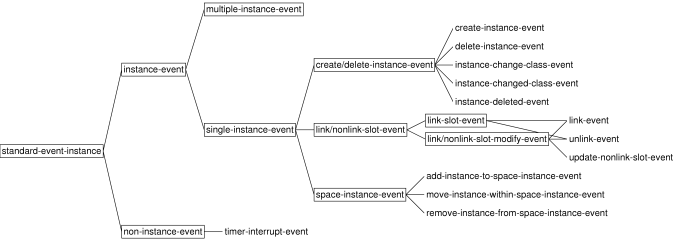
\includegraphics[scale=0.85]{gbbopen-events}
\end{center}
\W\end{iftex}

\noindent The event classes shown within rectangles are abstract classes
that cannot be signaled.

\W\xml{p}

Here are the defined event subclasses when both the \code{:gbbopen-core} and
\code{:agenda-shell} \glref{modules} have been loaded:
%
\T\begin{ifhtml}
\xml{br}
\xml{img align="center" src="agenda-shell-events.png"}
\xml{br clear="both"}
\T\end{ifhtml}
\W\begin{iftex} 
\begin{center}
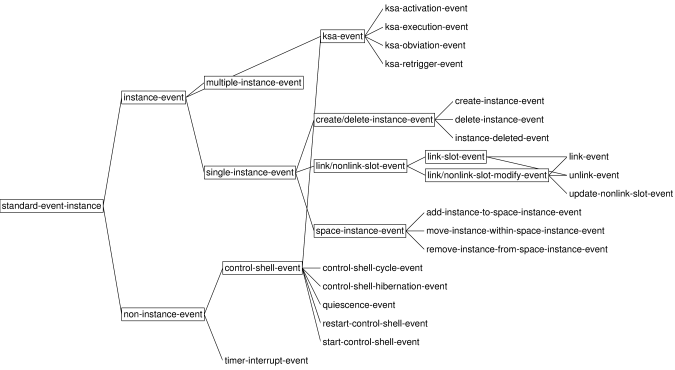
\includegraphics[scale=0.85]{agenda-shell-events}
\end{center}
\W\end{iftex}
%
The additional \code{control-shell-event} classes are defined and signaled by
the Agenda Shell.  Again classes shown within rectangles are abstract classes
that cannot be signaled.

\W\entities
\T\clearpage

%% ------------------------------------------------------------------------

\begin{functiondoc}{Function}{add-event-function}%
  {\var{function\/} [\var{event-class-specifier\/} 
    [\var{unit-class-or-instance-specifier\/}]] \\
    \code{\&key} \var{slot-names paths permanent priority\/}}
\index{event function!adding}%

%% Although the [] syntax is normally used for macros to denote optional
%% arguments, here we use them rather than &optional because of the 
%% keyword-driven argument parsing used in this function.

\fnsyntax

\fnpurpose Add an \glref{event~function} for one or more \glref{event~classes}.

\fnpackage \code{:gbbopen}

\fnmodule \code{:gbbopen-core}

\fnargs
\begin{args}{unit-class-or-instance-specifier}
\arg[function] A \glref{function~designator}
\arg[event-class-specifier] An \glref{extended~event-class~specification} 
(see below; default is \code{t})
\arg[unit-class-or-instance-specifier] An 
\glref{extended~unit-class~or~instance~specification} 
(see below; default is \code{t})
\arg[slot-names\/ \textrm{or} slot-name \T\hfil] A slot-name or list
of slot-names (default is \code{t})
\arg[paths\/ \textrm{or} path \T\hfil] A \glref{space-instance~path}
regular expression 
(default is \code{(*)})
\arg[permanent] A \glref{generalized~boolean} (default is \nil)
\arg[priority] An integer between -127 and 127, inclusive (default is \code{0})
\end{args}

\fndsyntax
\W\supp\tabletop
\eventclassspec
\subeventingspec
\syntaxsep
\unitclassinstancespec
\subclassingspec

\fndescription 
The specified \var{function\/} must accept the arguments associated with every
\glref{event~class} to which it is added.  In addition, \var{function\/}
should accept additional arguments that are associated with all
\glref{subevents} of the specified \glref{event~classes}. (This can be
achieved by specifying \code{\&allow-other-keys} in the lambda list of
\var{function}.)

The \var{paths\/} argument is either the symbol \code{t} (indicating
all \glref{space~instances}) or a list representing a regular
expression where the following reserved symbols are interpreted as
follows:
\spaceinstanceregexp

\begin{alsos}{remove-all-event-functions}
\also[remove-event-function]
\also[remove-all-event-functions]
\end{alsos}

\fnexamples
\bfindexit{evfn-printer}%
Add the event \glref{function} \entlink{evfn-printv} to the set of functions
to be invoked when \code{create-instance-event} is signaled on a
\code{hyp} \glref{unit~instance}:
%
\W\supp
\begin{example}
  (add-event-function 'evfn-printv 'create-instance-event 'hyp)
\end{example}
%
Add the event \glref{function} \entlink{evfn-printv} to the set of functions
to be invoked when \code{create-instance-event} is signaled on a
\code{hyp} \glref{unit~instance} or its subclasses:
%
\W\supp\notpretop
\begin{example}
  (add-event-function 'evfn-printv 'create-instance-event '(hyp :plus-subclasses))
\end{example}

\fnnote
\instanceevfnsnyi

\end{functiondoc}

%% ------------------------------------------------------------------------

\begin{functiondoc}{Macro}{define-event-class}{\var{event-class-name\/} 
   \code{(}\{\var{superclass-name\/}\}\superstar\code{)}
   [\var{documentation\/}] \\
   \code{(}\{\var{slot-specifier\/}\}\superstar\code{)}
   \{\var{class-option\/}\}\superstar{} 
   \returns{} \var{new-event-class\/}}
\index{event class!defining/redefining}%
\index{defining!an event class}%
\index{redefining!an event class}%

\fnsyntax

\fnpurpose Define or redefine an \glref{event~class}.

\fnpackage \code{:gbbopen}

\fnmodule \code{:gbbopen-core}

\fnargs
\begin{args}{event-class-name}
\arg[event-class-name] A non-\nil, \glref{non-keyword~symbol} that names the
\glref{event~class} 
\arg[superclass-name] A non-\nil, \glref{non-keyword~symbol} that specifies a
direct superclass of the \glref{event~class} \var{event-class-name\/}  
\arg[documentation] A documentation string
\arg[slot-specifiers] See below
\arg[class-options] See below
\arg[new-event-class] A new or modified \glref{event~class} object. 
\end{args}

\fnreturns The newly defined or modified \glref{event~class} object. 

\fndsyntax
\W\supp\tabletop
\begin{tabular}{@{~}l@{~}l}
\mbox{\var{slot-specifier\/} ::=}
 & \var{slot-name\/} \vbar{}
   \code{(}\var{slot-name\/} [[\var{slot-option\/}]]\code{)} \\
\end{tabular}
\T\\
\begin{tabular}{@{~}l@{~}l}
\mbox{\var{slot-option\/} ::=}
 & \{\code{:accessor} \var{reader-function-name\/}\}\superstar{} \vbar \\
 & \{\code{:allocation} \var{allocation-type\/}\} \vbar \\
 & \{\code{:documentation} \var{string\/}\} \vbar \\
 & \{\code{:initarg} \var{initarg-name\/}\}\superstar{} \vbar \\
 & \{\code{:initform} \var{form\/}\} \vbar \\
 & \{\code{:reader} \var{reader-function-name\/}\}\superstar{} \vbar \\
 & \{\code{:type} \var{type-specifier\/}\} \vbar{} \\
 & \{\code{:writer} \var{writer-function-name\/}\}\superstar{} \\
\end{tabular}
\T\\
\begin{tabular}{@{~}l@{~}l}
\mbox{\var{class-option\/} ::=}
 & \code{(:abstract} \var{boolean\/}\code{)} \vbar \\
 & \code{(:default-initargs .} \var{initarg-list\/}\code{)} \vbar \\
 & \code{(:documentation} \var{string\/}\code{)} \vbar \\
 & \code{(:event-metaclass} \var{event-metaclass-specifier\/}\code{)} \vbar \\
 & \code{(:event-printing} \var{event-printing-specifier\/}/code{)} \vbar \\
 & \code{(:export-class-name} \var{boolean\/}\code{)} \vbar \\
 & \code{(:export-accessors} \var{boolean\/}\code{)} \vbar \\
 & \code{(:generate-accessors} \var{direct-slots-specifier\/}\code{)} \vbar \\
 & \code{(:generate-accessors-format} 
     \{\code{:prefix} \vbar{} \code{:suffix}\} \vbar \\
 & \code{(:generate-accessors-prefix} \{\var{string\/} \vbar{}
     \var{symbol\/}\}\var\code{)} \vbar \\
 & \code{(:generate-accessors-suffix} \{\var{string\/} \vbar{}
     \var{symbol\/}\}\var\code{)} \vbar \\
 & \code{(:generate-initargs} \var{direct-slots-specifier\/}\code{)} \vbar \\
 & \code{(:metaclass} \var{class-name\/}\code{)} \\
\end{tabular}
\T\\
\begin{tabular}{@{~}l@{~}l}
\mbox{\var{event-metaclass-specifier\/} ::=}
  & non-instance-event-class \vbar{} instance-event-class \vbar{} \\
  & space-instance-event-class \vbar{} \\
  & nonlink-slot-event-class \vbar{} link-slot-event-class \\
\end{tabular}
\T\\
\begin{tabular}{@{~}l@{~}l}
\mbox{\var{direct-slots-specifier\/} ::=} & \nil{} \vbar{} \code{t} \vbar{}
  \var{included-slot-name\/}\superstar{} \vbar \\
  & \{\code{t :exclude} \var{excluded-slot-name\/}\superstar{}\} \\
\end{tabular}

\fnterms
\begin{args}{class-name}
\arg[class-name] A non-\nil, \glref{non-keyword~symbol} that names a
\glref{class} 
\arg[initarg-list] An \glref{initialization~argument~list}
\arg[slot-name] A non-\nil, \glref{non-keyword~symbol}
\end{args}

\fndescription 
\bfindexit{standard-event-class}%
Each \var{superclass-name} argument specifies a direct superclass of the new
class. If the superclass list is empty, then the direct superclass defaults to the
single class \textbf{\entlink{standard-event-instance}}.

\bfindexit{standard-event-class}%
The \code{:metaclass} \var{class-name\/} class option, if specified, must be a
subclass of \textbf{\entlinknoex{standard-event-class}}.  The default
metaclass value is the metaclass of the event superclasses of
\var{event-class-name} if they all have the same metaclass.  If the event
superclasses have multiple metaclasses, the metaclass of
\var{event-class-name} must be provided. The following table lists the
compatible event-superclass metaclasses for each \glref{event~metaclass}:

\begin{center}
\begin{tabular}{@{}l@{}l@{}c@{}l@{}c@{}l@{}c@{}l@{}c@{}l@{}c@{}}
& & \multicolumn{9}{c}{\textbf{Compatible Event-Superclass Metaclasses}}\\[4pt]
\multicolumn{1}{c}{\textbf{Event}}&~~~~~~&\code{non-}&~~&&~~&\code{space-}&~~& 
  \code{nonlink-}&~~&\code{link-}\\
\multicolumn{1}{c}{\textbf{Metaclass}}&&\code{instance}&&\code{instance}&&
   \code{instance}&&\code{slot}&&\code{slot}\\[4pt]
\code{non-instance-event-class}
   &&\textbf{X}&&          &&          &&          &&          \\
\code{instance-event-class}
   &&\textbf{X}&&\textbf{X}&&          &&          &&          \\
\code{space-instance-event-class}
   &&\textbf{X}&&\textbf{X}&&\textbf{X}&&          &&          \\
\code{nonlink-slot-event-class}
   &&\textbf{X}&&\textbf{X}&&          &&\textbf{X}&&          \\
\code{link-slot-event-class}
   &&\textbf{X}&&\textbf{X}&&          &&          &&\textbf{X}\\
\end{tabular}
\end{center}

The table in the documentation for \textbf{signal-event}
lists the \glref{initialization~arguments} that are required when
signaling an event.  These required \glref{initialization~arguments}
are based on the \glref{event~metaclass} of the \glref{event~class} of
the \glref{event} that is being signaled.

\begin{alsos}{with-generate-accessors-format}
\also[signal-event]
\also[standard-event-class]
\also[standard-event-instance]
\also[with-generate-accessors-format]
\end{alsos}

\bfindexit{non-instance-event}%
\fnexample
%
\W\supp
\begin{example}
> (define-event-class my-event (non-instance-event)
    ((my-event-arg1 :initform nil)
     (my-event-arg2 :initform nil)))
#<non-instance-event-class my-event>
\end{example}

\end{functiondoc}

%% ------------------------------------------------------------------------

\begin{functiondoc}{Function}{describe-event-printing}%
  {[\var{event-class-specifier\/} 
    [\var{unit-class-or-instance-specifier\/}]] \\
    \code{\&key} \var{slot-names paths\/}}
\index{event printing!printing information about}%
\index{printing!information about!event printing}%

%% Although the [] syntax is normally used for macros to denote optional
%% arguments, here we use them rather than &optional because of the 
%% keyword-driven argument parsing used in this function.

\fnsyntax

\fnpurpose Describe the printing of events for one or more
\glref{event~classes}. 

\fnpackage \code{:gbbopen}

\fnmodule \code{:gbbopen-core}

\fnargs
\begin{args}{unit-class-or-instance-specifier}
\arg[event-class-specifier] An \glref{extended~event-class~specification} 
(see below; default is \code{t})
\arg[unit-class-or-instance-specifier] An 
\glref{extended~unit-class~or~instance~specification} 
(see below; default is \code{t})
\arg[slot-names\/ \textrm{or} slot-name \T\hfil] A slot-name or list of
slot-names (default is \code{t})
\arg[paths\/ \textrm{or} path \T\hfil] A \glref{space-instance~path} regular
expression (default is \code{(*)})
\end{args}

\fndsyntax
\W\supp\tabletop
\eventclassspec
\subeventingspec
\syntaxsep
\unitclassinstancespec
\subclassingspec

\fndescription 
\bfindexit{*standard-output*}%
The \var{paths\/} argument is either the symbol \code{t} (indicating
all \glref{space~instances}) or a list representing a regular
expression where the following reserved symbols are interpreted as
follows:
\spaceinstanceregexp
The description is printed to the {\bf *standard-output*} stream.

\begin{alsos}{suspend-event-printing}
\also[disable-event-printing]
\also[enable-event-printing]
\also[resume-event-printing]
\also[suspend-event-printing]
\end{alsos}

\fnexample
Describe all event printing:
%
\W\supp
\begin{example}
> (describe-event-printing 'instance-event)
instance-event
  standard-unit-instance
  uc-2 [suspended]
  uc-1 [suspended]
  ksa
  ks
  root-space-instance
  standard-space-instance
\end{example}

\fnnote
\instanceevfnsnyi

\end{functiondoc}

%% ------------------------------------------------------------------------

\begin{functiondoc}{Function}{disable-event-printing}%
  {[\var{event-class-specifier\/} 
    [\var{unit-class-or-instance-specifier\/}]] \\
    \code{\&key} \var{slot-names paths\/}}
\index{event printing!disabling}%
\index{disabling!event printing}%

%% Although the [] syntax is normally used for macros to denote optional
%% arguments, here we use them rather than &optional because of the 
%% keyword-driven argument parsing used in this function.

\fnsyntax

\fnpurpose Disable the printing of events for one or more
\glref{event~classes}. 

\fnpackage \code{:gbbopen}

\fnmodule \code{:gbbopen-core}

\fnargs
\begin{args}{unit-class-or-instance-specifier}
\arg[event-class-specifier] An \glref{extended~event-class~specification} 
(see below; default is \code{t})
\arg[unit-class-or-instance-specifier] An 
\glref{extended~unit-class~or~instance~specification} 
(see below; default is \code{t})
\arg[slot-names\/ \textrm{or} slot-name \T\hfil] A slot-name or list of slot-names
(default is \code{t})
\arg[paths\/ \textrm{or} path \T\hfil] A \glref{space-instance~path} regular expression
(default is \code{(*)})
\end{args}

\fndsyntax
\W\supp\tabletop
\eventclassspec
\subeventingspec
\syntaxsep
\unitclassinstancespec
\subclassingspec

\fndescription 
The \var{paths\/} argument is either the symbol \code{t} (indicating
all \glref{space~instances}) or a list representing a regular
expression where the following reserved symbols are interpreted as
follows:
\spaceinstanceregexp

\begin{alsos}{describe-event-printing}
\also[describe-event-printing]
\also[enable-event-printing]
\also[resume-event-printing]
\also[suspend-event-printing]
\end{alsos}

\fnexample
Disable all event printing:
%
\W\supp
\begin{example}
  (disable-event-printing)
\end{example}

\fnnote
\instanceevfnsnyi

\end{functiondoc}

%% ------------------------------------------------------------------------

\begin{functiondoc}{Function}{enable-event-printing}%
{[\var{event-class-specifier\/} 
[\var{unit-class-or-instance-specifier\/}]] \\
\code{\&key} \var{slot-names paths\/}}
\index{event printing!enabling}%

%% Although the [] syntax is normally used for macros to denote optional
%% arguments, here we use them rather than &optional because of the 
%% keyword-driven argument parsing used in this function.

\fnsyntax

\fnpurpose Enable the printing of events for one or more \glref{event~classes}.

\fnpackage \code{:gbbopen}

\fnmodule \code{:gbbopen-core}

\fnargs
\begin{args}{unit-class-or-instance-specifier}
\arg[event-class-specifier] An \glref{extended~event-class~specification} 
(see below; default is \code{t})
\arg[unit-class-or-instance-specifier] An 
\glref{extended~unit-class~or~instance~specification} 
(see below; default is \code{t})
\arg[slot-names\/ \textrm{or} slot-name \T\hfil] A slot-name or list of slot-names
(default is \code{t})
\arg[paths\/ \textrm{or} path \T\hfil] A \glref{space-instance~path} regular expression
(default is \code{(*)})
\end{args}

\fndsyntax
\W\supp\tabletop
\eventclassspec
\subeventingspec
\syntaxsep
\unitclassinstancespec
\subclassingspec

\fndescription 
The \var{paths\/} argument is either the symbol \code{t} (indicating
all \glref{space~instances}) or a list representing a regular
expression where the following reserved symbols are interpreted as
follows:
\spaceinstanceregexp

\begin{alsos}{describe-event-printing}
\also[describe-event-printing]
\also[disable-event-printing]
\also[resume-event-printing]
\also[suspend-event-printing]
\end{alsos}

\fnexample
Enable event printing on all \glref{space-instance} events of
\code{hyp} \glref{unit~instances}:
%
\W\supp
\begin{example}
  (enable-event-printing '(space-instance-event :plus-subevents)
                         '(hyp :plus-subclasses))
\end{example}

\fnnote
\instanceevfnsnyi

\end{functiondoc}

%% ------------------------------------------------------------------------

\begin{functiondoc}{Function}{evfn-printv}{\var{event-class\/} 
    \&rest \var{args\/}}
\index{debugging, using evfn-printv@using \textbf{evfn-printv}}% 

\fnsyntax

\fnpurpose Assist debugging by printing forms and the results of
evaluating them to \code{*trace-output*}.

\fnpackage \code{:gbbopen}

\fnmodule \code{:gbbopen-core}

\fnargs
\begin{args}{results}
\arg[forms] An implicit \textbf{progn} of \glref{forms} to be
evaluated and printed  
\end{args}

\fnreturns The values returned by evaluating the last \var{form}.

\fndescription Evaluates \var{forms\/}, printing the \var{form\/} and the
result values of each evaluation to \code{*trace-output*}.  Any\var{form\/}
that is a string (before evaluation) is simply printed without enclosing
double-quote characters.

\fnexamples
\bfindexit{evfn-printer}%
Add the event \glref{function} \entlink{evfn-printv} to the set of functions
to be invoked when \code{create-instance-event} is signaled on a
\code{hyp} \glref{unit~instance}:
%
\W\supp
\begin{example}
  (add-event-function 'evfn-printv 'create-instance-event 'hyp)
\end{example}

\end{functiondoc}

%% ------------------------------------------------------------------------

\begin{functiondoc}{Function}{remove-all-event-functions}%
{[\var{event-class-specifier\/} 
[\var{unit-class-or-instance-specifier\/}]] \\
\code{\&key} \var{slot-names paths permanent\/}}
\index{event function!removing all}%

%% Although the [] syntax is normally used for macros to denote optional
%% arguments, here we use them rather than &optional because of the 
%% keyword-driven argument parsing used in this function.

\fnsyntax

\fnpurpose Remove all \glref{event~functions} for one or more \glref{event~classes}.

\fnpackage \code{:gbbopen}

\fnmodule \code{:gbbopen-core}

\fnargs
\begin{args}{unit-class-or-instance-specifier}
\arg[event-class-specifier] An \glref{extended~event-class~specification} 
(see below; default is \code{t})
\arg[unit-class-or-instance-specifier] An 
\glref{extended~unit-class~or~instance~specification}
(see below; default is \code{t})
\arg[slot-names\/ \textrm{or} slot-name \T\hfil] A slot-name or list of slot-names
(default is \code{t})
\arg[paths\/ \textrm{or} path \T\hfil] A \glref{space-instance~path} regular expression
(default is \code{(*)})
\arg[permanent] A \glref{generalized~boolean} (default is \nil)
\end{args}

\fndsyntax
\W\supp\tabletop
\eventclassspec
\subeventingspec
\syntaxsep
\unitclassinstancespec
\subclassingspec

\begin{alsos}{remove-event-function}
\also[add-event-function]
\also[remove-event-function]
\end{alsos}

\fnexamples
\bfindexit{evfn-printer}%
Remove all event functions associated with a
\code{create-instance-event} on a \code{hyp} \glref{unit~instance}:
%
\W\supp
\begin{example}
  (remove-all-event-functions 'create-instance-event 'hyp)
\end{example}
%
Remove all event functions associated with a
\code{create-instance-event} on a \code{hyp} \glref{unit~instance} or
its subclasses:
%
\W\supp\notpretop
\begin{example}
  (remove-all-event-functions 'create-instance-event '(hyp :plus-subclasses))
\end{example}

\fnnote
\instanceevfnsnyi

\end{functiondoc}

%% ------------------------------------------------------------------------

\begin{functiondoc}{Function}{remove-event-function}%
{\var{function\/} [\var{event-class-specifier\/} 
[\var{unit-class-or-instance-specifier\/}]] \\
\code{\&key} \var{slot-names paths permanent\/}}
\index{event function!removing}%

%% Although the [] syntax is normally used for macros to denote optional
%% arguments, here we use them rather than &optional because of the 
%% keyword-driven argument parsing used in this function.

\fnsyntax

\fnpurpose Remove an \glref{event~function} for one or more \glref{event~classes}.

\fnpackage \code{:gbbopen}

\fnmodule \code{:gbbopen-core}

\fnargs
\begin{args}{space-instance}
\arg[function] A \glref{function~designator}
\arg[event-class-specifier] An \glref{extended~event-class~specification} 
(see below; default is \code{t})
\arg[unit-class-or-instance-specifier] An 
\glref{extended~unit-class~or~instance~specification}
(see below; default is \code{t})
\arg[slot-names\/ \textrm{or} slot-name \T\hfil] A slot-name or list of slot-names
(default is \code{t})
\arg[paths\/ \textrm{or} path \T\hfil] A \glref{space-instance~path} regular expression
(default is \code{(*)})
\arg[permanent] A \glref{generalized~boolean} (default is \nil)
\end{args}

\fndsyntax
\W\supp\tabletop
\eventclassspec
\subeventingspec
\syntaxsep
\unitclassinstancespec
\subclassingspec

\begin{alsos}{remove-all-event-functions}
\also[add-event-function]
\also[remove-all-event-functions]
\end{alsos}

\fnexamples
\bfindexit{evfn-printer}%
Remove the event \glref{function} \entlink{evfn-printv} from the set of functions
to be invoked when \code{create-instance-event} is signaled on a
\code{hyp} \glref{unit~instance}:
%
\W\supp
\begin{example}
  (remove-event-function 'evfn-printv 'create-instance-event 'hyp)
\end{example}
%
Remove the event \glref{function} \entlink{evfn-printv} from the set of
functions to be invoked when \code{create-instance-event} is signaled on a
\code{hyp} \glref{unit~instance} or its subclasses:
%
\W\supp\notpretop
\begin{example}
  (remove-event-function 'evfn-printv 'create-instance-event '(hyp :plus-subclasses))
\end{example}

\fnnote
\instanceevfnsnyi

\end{functiondoc}

%% ------------------------------------------------------------------------

\begin{functiondoc}{Function}{resume-event-printing}%
{[\var{event-class-specifier\/} 
[\var{unit-class-or-instance-specifier\/}]] \\
\code{\&key} \var{slot-names paths\/}}
\index{event printing!resuming}%

%% Although the [] syntax is normally used for macros to denote optional
%% arguments, here we use them rather than &optional because of the 
%% keyword-driven argument parsing used in this function.

\fnsyntax

\fnpurpose Resume the printing of printing-enabled events for one or more
\glref{event~classes}. 

\fnpackage \code{:gbbopen}

\fnmodule \code{:gbbopen-core}

\fnargs
\begin{args}{unit-class-or-instance-specifier}
\arg[event-class-specifier] An \glref{extended~event-class~specification} 
(see below; default is \code{t})
\arg[unit-class-or-instance-specifier] An 
\glref{extended~unit-class~or~instance~specification} 
(see below; default is \code{t})
\arg[slot-names\/ \textrm{or} slot-name \T\hfil] A slot-name or list of slot-names
(default is \code{t})
\arg[paths\/ \textrm{or} path \T\hfil] A \glref{space-instance~path} regular expression
(default is \code{(*)})
\end{args}

\fndsyntax
\W\supp\tabletop
\eventclassspec
\subeventingspec
\syntaxsep
\unitclassinstancespec
\subclassingspec

\fndescription 
The \var{paths\/} argument is either the symbol \code{t} (indicating
all \glref{space~instances}) or a list representing a regular
expression where the following reserved symbols are interpreted as
follows:
\spaceinstanceregexp

\begin{alsos}{describe-event-printing}
\also[describe-event-printing]
\also[disable-event-printing]
\also[enable-event-printing]
\also[suspend-event-printing]
\end{alsos}

\fnexample
Resume all suspended event printing:
%
\W\supp
\begin{example}
  (resume-event-printing)
\end{example}

\fnnote
Resuming event printing does not enable event printing that is disabled.

\instanceevfnsnyi

\end{functiondoc}

%% ------------------------------------------------------------------------

\begin{functiondoc}{Function}{signal-event}{\var{event-class\/}
  \code{\&rest} \var{initargs\/}}
\index{event!signaling}%
\index{signaling!an event}%

\fnsyntax

\fnpurpose Signal an event

\fnpackage \code{:gbbopen}

\fnmodule \code{:gbbopen-core}

\fnargs
\begin{args}{initargs}
\arg[event-class] An \glref{event~class} or a non-\nil, \glref{non-keyword~symbol} that 
names an \glref{event~class} 
\arg[initargs] An \glref{initialization~argument~list}
\end{args}

\fndescription

\index{event function!required arguments}%
\index{function!event!required arguments}%
The following table lists the \glref{initialization~arguments} that
are required for specific event metaclasses:
\begin{center}
  \begin{tabular}{@{}l@{}l@{}}
  \textbf{Event metaclass} & \textbf{Required initargs} \\ \hline
  \code{non-instance-event-class} 
  & None \\
  \code{instance-event-class} 
  & \code{:instance} \var{unit-instance\/} \\
  \code{space-instance-event-class}~~~~~
  & \code{:instance} \var{unit-instance\/} \\
  & \code{:space-instance} \var{space-instance\/} \\ 
  \code{nonlink-slot-event-class}
  & \code{:instance} \var{unit-instance\/} \\
  & \code{:slot} \var{effective-nonlink-slot-definition\/} \\
  \code{link-slot-event-class}
  & \code{:instance} \var{unit-instance\/} \\
  & \code{:slot} \var{effective-link-definition\/} \\ \hline
\end{tabular}
\end{center}

\begin{alsos}{with-events-disabled}
\also[define-event-class]
\also[with-events-disabled]
\also[with-events-enabled]
\end{alsos}

\fnexample
%
\W\supp
\begin{example}
  (signal-event 'my-event :my-event-arg1 3)
\end{example}
\end{functiondoc}

%% ------------------------------------------------------------------------

\begin{functiondoc}{Class}{standard-event-class}{}
\index{class!standard-event-class@\textbf{standard-event-class}}%

\fnsyntax

\fnpackage \code{:gbbopen}

\fnmodule \code{:gbbopen-core}

\fndescription 
\bfindexit{define-event-class}%
The class \textbf{standard-event-class} is the superclass of classes defined
by \textbf{\entlinknoex{define-event-class}}.  It is a subclass of
\code{standard-class}.

\begin{alsos}{standard-event-instance}
\also[define-event-class]
\also[standard-event-instance]
\end{alsos}

\end{functiondoc}

%% ------------------------------------------------------------------------

\begin{functiondoc}{Event~Class}{standard-event-instance}{}
\index{class!standard-event-instance@\textbf{standard-event-instance}}%
\index{event class!standard-event-instance@\textbf{standard-event-instance}}%
  
\fnsyntax

\fnpackage \code{:gbbopen}

\fnmodule \code{:gbbopen-core}

\fndescription 
\bfindexit{standard-event-class}%
The class \textbf{standard-event-instance} is an \glref{instance} of
\textbf{\entlinknoex{standard-event-class}} and is a superclass of every
\glref{event~class} that is an \glref{instance} of
\textbf{\entlinknoex{standard-event-class}} except itself.  It is a subclass
of \textbf{\glref{standard-gbbopen-instance}}.

\begin{alsos}{standard-event-class}
\also[print-instance-slots]
\also[standard-gbbopen-instance]
\also[standard-event-class]
\end{alsos}

\end{functiondoc}

%% ------------------------------------------------------------------------

\begin{functiondoc}{Function}{suspend-event-printing}%
{[\var{event-class-specifier\/} 
[\var{unit-class-or-instance-specifier\/}]] \\
\code{\&key} \var{slot-names paths\/}}
\index{event printing!suspending}%

%% Although the [] syntax is normally used for macros to denote optional
%% arguments, here we use them rather than &optional because of the 
%% keyword-driven argument parsing used in this function.

\fnsyntax

\fnpurpose Suspend the printing of printing-enabled events for one or more
\glref{event~classes}. 

\fnpackage \code{:gbbopen}

\fnmodule \code{:gbbopen-core}

\fnargs
\begin{args}{unit-class-or-instance-specifier}
\arg[event-class-specifier] An \glref{extended~event-class~specification} 
(see below; default is \code{t})
\arg[unit-class-or-instance-specifier] An 
\glref{extended~unit-class~or~instance~specification} 
(see below; default is \code{t})
\arg[slot-names\/ \textrm{or} slot-name \T\hfil] A slot-name or list of slot-names
(default is \code{t})
\arg[paths\/ \textrm{or} path \T\hfil] A \glref{space-instance~path} regular expression
(default is \code{(*)})
\end{args}

\fndsyntax
\W\supp\tabletop
\eventclassspec
\subeventingspec
\syntaxsep
\unitclassinstancespec
\subclassingspec

\fndescription 
Suspending event printing is a convenient way of switching off event
printing without losing event-printing enabled/disabled settings.
Disabled event printing remains disabled if event printing is
resumed (by using \textbf{\entlinknoex{resume-event-printing}}).

The \var{paths\/} argument is either the symbol \code{t} (indicating
all \glref{space~instances}) or a list representing a regular
expression where the following reserved symbols are interpreted as
follows:
\spaceinstanceregexp

\begin{alsos}{describe-event-printing}
\also[describe-event-printing]
\also[disable-event-printing]
\also[enable-event-printing]
\also[resume-event-printing]
\end{alsos}

\fnexample
Suspend all event printing associated with \code{possible-hyp}
\glref{unit~instances}: 
%
\W\supp
\begin{example}
  (suspend-event-printing 't 'possible-hyp)
\end{example}

\fnnote
\instanceevfnsnyi

\end{functiondoc}

%% ------------------------------------------------------------------------

\begin{functiondoc}{Macro}{with-events-disabled}%
  {\code{(}\var{option\/}\superstar{}\code{)}
    \var{declaration\/}\superstar{}
    \var{form\/}\superstar{}
    \returns{} \var{result\/}\superstar}
\index{disabling!event signaling}%
\index{events!disabling signaling of}%
  
\fnsyntax

\fnpurpose Disable event signaling during evaluation of \var{forms}.

\fnpackage \code{:gbbopen}

\fnmodule \code{:gbbopen-core}

\fnargs
\begin{args}{options}
\arg[option] No options are currently supported
\arg[declaration] A declare expression
\arg[forms] An implicit \textbf{progn} of \glref{forms} to be evaluated
\arg[results] The values returned by evaluating the last \var{form}
\end{args}

\fnreturns The values returned by evaluating the last \var{form}.

\begin{alsos}{with-events-enabled}
\also[signal-event]
\also[with-events-enabled]
\end{alsos}

\fnexample
\bfindexit{make-instance}%
Create a \code{hyp} without signaling any events:
%
\W\supp
\begin{example}
> (with-events-disabled ()
     (\entlink{make-instance} 'hyp 
        :location (list x y)
        :classification '(:car :truck)
        :color ':red
        :belief .85
        :velocity-range '(5 35)
        :supporting-hyps supporting-hyps))
#<hyp 419 (1835 4791) 0.85 [5..35]>
\end{example}

\end{functiondoc}

%% ------------------------------------------------------------------------

\begin{functiondoc}{Macro}{with-events-enabled}%
  {\code{(}\var{option\/}\superstar{}\code{)}
    \var{declaration\/}\superstar{}
    \var{form\/}\superstar{}
    \returns{} \var{result\/}\superstar}
\index{enabling event signaling}%
\index{events!enabling signaling of}%
  
\fnsyntax

\fnpurpose Restore event signaling during evaluation of \var{forms}.

\fnpackage \code{:gbbopen}

\fnmodule \code{:gbbopen-core}

\fnargs
\begin{args}{options}
\arg[option] No options are currently supported
\arg[declaration] A declare expression
\arg[forms] An implicit \textbf{progn} of \glref{forms} to be evaluated
\arg[results] The values returned by evaluating the last \var{form}
\end{args}

\fnreturns The values returned by evaluating the last \var{form}.

\begin{alsos}{with-events-disabled}
\also[signal-event]
\also[with-events-disabled]
\end{alsos}

\fnexample
\bfindexit{make-instance}%
Create a \code{hyp} without signaling any events, then add
supporting-hypothesis links with events enabled:
%
\W\supp
\begin{example}
> (\entlink{with-events-disabled}
     (let ((hyp (\entlink{make-instance} 'hyp 
                   :location (list x y)
                   :classification '(:car :truck)
                   :color ':red
                   :belief .85
                   :velocity-range '(5 35))))
        (with-events-enabled ()
           (linkf (supporting-hyps-of hyp) supporting-hyps))
        hyp))
#<hyp 419 (1835 4791) 0.85 [5..35]>
\end{example}

\end{functiondoc}

%% ------------------------------------------------------------------------

\T\markright{}%
\T\pagestyle{plain}
\T\clearpage
\W\xname{ref-interval-entities}
\T\pagestyle{fancy}
\T\thispagestyle{fancybottom}
\T\global\def\fnlastname{ }%

\subsection{Intervals}
\label{sec:interval}%

This section contains \code{:gbbopen-core} entities that pertain to
\glref{intervals}. An interval $[a,b]$ is the set of real numbers between the
start value of the interval, $a$, and the end value, $b$, inclusive. The
interval $[x,x]$ represents the single point $x$.

An interval is represented as either a \glref{cons}, a two-element list, or a
two-element array containing the start and end values of the interval.  So, a
representation for the interval $[0,100]$ can be created as any of the
following:
\begin{tightitemize}
\item \code{(cons 0 100)}
\item \code{(list 0 100)}
\item \code{(vector 0 100)}
\end{tightitemize}
%
The function \textbf{\entlink{make-interval}} is provided for stylistic
clarity in creating an interval.

\bfindexit{make-interval}%
%
Intervals also include the unbounded intervals:
\begin{tightitemize}
\item $(-\infty,\infty)$ ~ (provided as the constant 
  \textbf{\entlink{infinite-interval}})
\item $(-\infty,x]$      ~ (for example, 
   \code{(\entlink{make-interval} x infinity)})
\item $[x,\infty)$       ~ (for example, 
   \code{(\entlink{make-interval} -infinity x)})
\end{tightitemize}

It is an error for the start value of an interval to be greater than the end
value.

\W\entities
\T\clearpage

%% ------------------------------------------------------------------------

\begin{functiondoc}[coerce-contracted-interval-rationals-to-floats-var]%
  {Variable}%
  {*coerce-contracted-interval-rationals-to-floats*}{}%

\fnsyntax

\fnpurpose Control automatic coercion of non-integer rationals to floats when
an interval is contracted into a non-integral point range by
\textbf{\entlink{expand-interval}} and \textbf{\entlink{nexpand-interval}}.

\fnpackage \code{:gbbopen}

\fnmodule \code{:gbbopen-core}

\fnvaluetype A \glref{generalized~boolean}

\fninitialvalue \nil{}

\begin{alsos}{nexpand-interval}
\also[expand-interval]
\also[nexpand-interval]
\end{alsos}

\fnexamples
%
\bfindexit{expand-interval}%
%
\W\supp
\begin{example}
> (let ((*coerce-contracted-interval-rationals-to-floats* 't))
     (expand-interval '(2 . 5) -3))
(3.5 . 3.5)
> (let ((*coerce-contracted-interval-rationals-to-floats* nil))
     (expand-interval '(2 . 5) -3))
(7/2 . 7/2)
>
\end{example}

\end{functiondoc}

%% ------------------------------------------------------------------------

\begin{functiondoc}{Function}{copy-interval}%
  {\var{interval\/}
    \returns{} \var{new-interval\/}}
\index{copy, an interval}%
\index{interval!copying}%

\fnsyntax

\fnpurpose Create a new \glref{interval} by copying \var{interval}.

\fnpackage \code{:gbbopen}

\fnmodule \code{:gbbopen-core}

\fnargs
\begin{args}{new-interval}
\arg[interval] An \glref{interval}
\arg[new-interval] An \glref{interval}
\end{args}

\fnreturns The new \glref{interval}.

\fndescription The structure of the original \var{interval\/} (\glref{cons},
two-element list, or two-element array) is maintained in the newly allocated
\var{new-interval}.

\begin{alsos}{infinite-interval}
\also[expand-interval]
\also[infinite-interval]
\also[interval-start]
\also[interval-end]
\also[make-interval]
\also[nexpand-interval]
\also[nshift-interval]
\also[shift-interval]
\end{alsos}

\fnexamples
%
\W\supp
\begin{example}
> (copy-interval '(2 5))
(2 5)
> (copy-interval '(2 . 5))
(2 . 5)
> (expand-interval #(2 5))
#(2 5)
\end{example}

\end{functiondoc}

%% ------------------------------------------------------------------------

\begin{functiondoc}{Function}{expand-interval}%
  {\var{interval amount\/}
    \returns{} \var{new-interval\/}}
\index{expand, an interval}%
\index{interval!expanding}%

\fnsyntax

\fnpurpose Create a new \glref{interval} by expanding \var{interval\/} by
\var{amount}.

\fnpackage \code{:gbbopen}

\fnmodule \code{:gbbopen-core}

\fnargs
\begin{args}{new-interval}
\arg[interval] An \glref{interval}
\arg[amount] A numbe
\arg[new-interval] An \glref{interval}
\end{args}

\fnreturns A new, expanded \glref{interval}.

\fndescription The structure of the original \var{interval\/}
(\glref{cons}, two-element list, or two-element array) is maintained in the
newly allocated, expanded \var{new-interval}.

An interval that is contracted (expanded negatively) by an amount greater than
one-half of its width will result in a zero-width \var{new-interval\/} at the
center point of the original \var{interval}.

\begin{alsos}{*coerce-contracted-interval-rationals-to-floats*}
\also[*coerce-contracted-interval-rationals-to-floats*]
\also[copy-interval]
\also[infinite-interval]
\also[interval-start]
\also[interval-end]
\also[interval-values]
\also[make-interval]
\also[nexpand-interval]
\also[nshift-interval]
\also[shift-interval]
\end{alsos}

\fnexamples
%
\W\supp
\begin{example}
> (expand-interval '(2 5) 2)
(0 7)
> (expand-interval '(2 . 5) -1)
(3 . 4)\goodpagebreak
> (expand-interval #(2 5) .5)
#(1.5 5.5)
> (expand-interval '(2 . 5) -3)
(3.5 . 3.5)
\end{example}

\end{functiondoc}

%% ------------------------------------------------------------------------

\begin{functiondoc}{Function}{expand-point}%
  {\var{point amount\/}
    \code{\&optional} \var{type-specifier\/} 
    \returns{} \var{new-interval\/}}
\index{expand, a point into an interval}%
\index{point!expanding into an interval}%

\fnsyntax

\fnpurpose Create a new \glref{interval} by expanding \var{point\/} by
\var{amount}.

\fnpackage \code{:gbbopen}

\fnmodule \code{:gbbopen-core}

\fnargs
\begin{args}{type-specifier}
\arg[point] A number
\arg[amount] A number
\arg[type-specifier] One of: \code{cons}, \code{list}, or \code{array}.
  (Default is \code{cons}.)
\arg[new-interval] An \glref{interval}
\end{args}

\fnreturns The new \glref{interval}.

\begin{alsos}{nexpand-interval}
\also[expand-interval]
\also[interval-start]
\also[interval-end]
\also[interval-values]
\also[make-interval]
\also[nexpand-interval]
\also[nshift-interval]
\also[shift-interval]
\end{alsos}

\fnexamples
%
\W\supp
\begin{example}
> (expand-point 3 2)
(1 . 5)
> (expand-point 3 2 'cons)
(1 . 5)
> (expand-point 3 2 'list)
(1 5)
> (expand-point 3 2 'array)
#(1 5)
\end{example}

\fnnote
%
\bfindex{expand-point\&}%
\bfindex{expand-point\$\&}%
\bfindex{expand-point\$}%
\bfindex{expand-point\$\$}%
\bfindex{expand-point\$\$\$}%
%
\reflink{Declared numeric}{sec:declared-numerics} versions of
\textbf{expand-point} are also provided: \textbf{expand-point\&},
\textbf{expand-point\$\&}, \textbf{expand-point\$},
\textbf{expand-point\$\$}, and \textbf{expand-point\$\$\$}.

\end{functiondoc}

%% ------------------------------------------------------------------------

\begin{functiondoc}{Constant}{infinite-interval}{}%

\fnsyntax

\fnpurpose An interval (represented as a cons) from \code{-infinity} to
\code{infinity}.

\fnpackage \code{:gbbopen}

\fnmodule \code{:gbbopen-core}

\begin{alsos}{nexpand-interval}
\also[copy-interval]
\also[expand-interval]
\also[interval-end]
\also[interval-start]
\also[interval-values]
\also[make-interval]
\also[nexpand-interval]
\also[nshift-interval]
\also[shift-interval]
\end{alsos}

\fnexample
%
\bfindexit{define-unit-class}%
\bfindexit{copy-interval}%
%
Define a \glref{unit~class}, \code{temporal-duration-mixin}, that contains a
\code{temporal-duration} slot and \glref{dimension~value} declaration:
%
\W\supp
\begin{example}
> (define-unit-class temporal-duration-mixin ()
    ((temporal-duration 
       ;; Copy the interval to allow destructive changes by
       ;; GBBopen's interval operators:
       :initform (copy-interval infinite-interval)))
    (:dimensional-values
     (temporal-duration :interval temporal-duration)))
#<standard-unit-class temporal-duration-mixin>
\end{example}

\end{functiondoc}

%% ------------------------------------------------------------------------

\begin{functiondoc}{Function}{interval-end}%
  {\var{interval\/}
    \returns{} \var{end-value\/}}
\index{end value, of an interval}%
\index{interval!obtaining the end value}%

\fnsyntax

\fnpurpose Obtain the end value of an \glref{interval}.

\fnsetf
\fnsetfsyntax{interval-end}{\var{interval\/}}{\var{end-value\/}}

\fnpackage \code{:gbbopen}

\fnmodule \code{:gbbopen-core}

\fnargs
\begin{args}{interval}
\arg[interval] An \glref{interval}
\arg[end-value] A number
\end{args}

\fnreturns The end value of the \glref{interval}.

\begin{alsos}{interval-values}
\also[interval-start]
\also[interval-values]
\end{alsos}

\fnexamples
%
\bfindexit{make-interval}
%
\W\supp
\begin{example}
> (interval-end '(1 2))
2
> (interval-end '(1 . 2))
2
> (interval-end #(1  2))
2\goodpagebreak
> (defparameter *x* (\entlink{make-interval} 1 2))
(1 . 2)
> (setf (interval-end *x*) 4)
4
> *x*
(1 . 4)
\end{example}

\end{functiondoc}

%% ------------------------------------------------------------------------

\begin{functiondoc}{Function}{interval-start}%
  {\var{interval\/} 
    \returns{} \var{start-value\/}}
\index{start value, of an interval}%
\index{interval!obtaining the start value}%

\fnsyntax

\fnpurpose Obtain the start value of an \glref{interval}.

\fnsetf
\fnsetfsyntax{interval-start}{\var{interval\/}}{\var{start-value\/}}

\fnpackage \code{:gbbopen}

\fnmodule \code{:gbbopen-core}

\fnargs
\begin{args}{interval}
\arg[interval] An \glref{interval}
\arg[start-value] A number
\end{args}

\fnreturns The start value of the \glref{interval}.

\begin{alsos}{interval-values}
\also[interval-end]
\also[interval-values]
\end{alsos}

\fnexamples
%
\bfindexit{make-interval}
%
\W\supp
\begin{example}
> (interval-start '(1 2))
1
> (interval-start '(1 . 2))
1
> (interval-start #(1 2))
1\goodpagebreak
> (defparameter *x* (\entlink{make-interval} 1 2))
(1 . 2)
> (setf (interval-start *x*) -1)
-1
> *x*
(-1 . 4)

\end{example}

\end{functiondoc}

%% ------------------------------------------------------------------------

\begin{functiondoc}{Function}{interval-values}%
  {\var{interval\/} 
    \returns{} \var{start-value, end-value\/}}
\index{start value, of an interval}%
\index{end value, of an interval}%
\index{values, start and end, of an interval}%
\index{interval!obtaining the start value}%
\index{interval!obtaining the end value}%
\index{interval!obtaining the start and end values}%

\fnsyntax

\fnpurpose Obtain the start and end values of an \glref{interval}.

\fnsetf
\fnsetfsyntax{interval-values}{\var{interval\/}}{\var{source-interval\/}}

\fnpackage \code{:gbbopen}

\fnmodule \code{:gbbopen-core}

\fnargs
\begin{args}{source-interval}
\arg[interval] An \glref{interval}
\arg[source-interval] An \glref{interval}
\arg[start-value] A number
\arg[end-value] A number
\end{args}

\fnreturns Two values: the start value and the end value of the \glref{interval}.

\begin{alsos}{interval-start}
\also[interval-end]
\also[interval-start]
\end{alsos}

\fnexamples
%
\bfindexit{make-interval}
%
\W\supp
\begin{example}
> (interval-values '(1 2))
1
2
> (interval-values '(1 . 2))
1
2
> (interval-values #(1  2))
1
2\goodpagebreak
> (defparameter *x* (\entlink{make-interval} 1 2))
(1 . 2)
> (setf (interval-values *x*) #(3 4))
#(3 4)
> *x*
(3 . 4)
\end{example}

\end{functiondoc}

%% ------------------------------------------------------------------------

\begin{functiondoc}{Function}{make-interval}%
  {\var{start end\/} 
    \code{\&optional} \var{type-specifier\/} 
    \returns{} \var{new-interval\/}}
\index{make, an interval}%
\index{interval!making}%

\fnsyntax

\fnpurpose Create a new \glref{interval} of type \var{type-specifier}.

\fnpackage \code{:gbbopen}

\fnmodule \code{:gbbopen-core}

\fnargs
\begin{args}{type-specifier}
\arg[start] A number
\arg[end] A number
\arg[type-specifier] One of: \code{cons}, \code{list}, or \code{array}.
  (Default is \code{cons}.)
\arg[new-interval] An \glref{interval}
\end{args}

\fnreturns The new \glref{interval}.

\begin{alsos}{infinite-interval}
\also[copy-interval]
\also[expand-interval]
\also[expand-point]
\also[infinite-interval]
\also[interval-start]
\also[interval-end]
\also[nexpand-interval]
\also[nshift-interval]
\also[shift-interval]
\end{alsos}

\fnexamples
%
\W\supp
\begin{example}
> (make-interval 2 5)
(2 . 5)
> (make-interval 2 5 'list)
(2 5)
> (make-interval 2 5 'cons)
(2 . 5)
> (make-interval 2 5 'array)
#(2 5)
\end{example}

\end{functiondoc}

%% ------------------------------------------------------------------------

\begin{functiondoc}{Function}{nexpand-interval}%
  {\var{interval amount\/}
    \returns{} \var{interval\/}}
\index{expand, an interval}%
\index{interval!expanding}%

\fnsyntax

\fnpurpose Expand an \glref{interval} by \var{amount}.

\fnpackage \code{:gbbopen}

\fnmodule \code{:gbbopen-core}

\fnargs
\begin{args}{interval}
\arg[interval] An \glref{interval}
\arg[amount] A number
\end{args}

\fnreturns The expanded \var{interval}.

\fndescription An interval that is contracted (expanded negatively) by an
amount greater than one-half of its width will result in a zero-width
\var{interval\/} at the center point of the original \var{interval}.

\begin{alsos}{*coerce-contracted-interval-rationals-to-floats*}
\also[*coerce-contracted-interval-rationals-to-floats*]
\also[copy-interval]
\also[expand-interval]
\also[expand-point]
\also[infinite-interval]
\also[interval-start]
\also[interval-values]
\also[interval-end]
\also[make-interval]
\also[nshift-interval]
\also[shift-interval]
\end{alsos}

\fnexamples
%
\W\supp
\begin{example}
> (nexpand-interval '(2 5) 2)
(0 7)
> (nexpand-interval '(2 . 5) -1)
(3 . 4)\goodpagebreak
> (nexpand-interval #(2 5) .5)
#(1.5 5.5)
> (nexpand-interval '(2 . 5) -3)
(3.5 . 3.5)
\end{example}

\end{functiondoc}

%% ------------------------------------------------------------------------

\begin{functiondoc}{Function}{nshift-interval}%
  {\var{interval amount\/}
    \returns{} \var{interval\/}}
\index{shift, an interval}%
\index{interval!shifting}%

\fnsyntax

\fnpurpose Shift an \glref{interval} by \var{amount}.

\fnpackage \code{:gbbopen}

\fnmodule \code{:gbbopen-core}

\fnargs
\begin{args}{interval}
\arg[interval] An \glref{interval}
\arg[amount] A number
\end{args}

\fnreturns The shifted \var{interval}.

\begin{alsos}{infinite-interval}
\also[copy-interval]
\also[expand-interval]
\also[expand-point]
\also[infinite-interval]
\also[interval-end]
\also[interval-start]
\also[interval-values]
\also[make-interval]
\also[nexpand-interval]
\also[shift-interval]
\end{alsos}

\fnexamples
%
\W\supp
\begin{example}
> (nshift-interval '(2 5) 2)
(4 7)
> (nshift-interval '(2 . 5) -1)
(1 . 4)
> (nshift-interval #(2 5) .5)
#(2.5 5.5)
\end{example}

\end{functiondoc}

%% ------------------------------------------------------------------------

\begin{functiondoc}{Function}{shift-interval}%
  {\var{interval amount\/}
    \returns{} \var{new-interval\/}}
\index{shift, an interval}%
\index{interval!shifting}%

\fnsyntax

\fnpurpose Create a new \glref{interval} by shifting \var{interval\/} by
\var{amount}.

\fnpackage \code{:gbbopen}

\fnmodule \code{:gbbopen-core}

\fnargs
\begin{args}{new-interval}
\arg[interval] An \glref{interval}
\arg[amount] A number
\arg[new-interval] An \glref{interval}
\end{args}

\fnreturns A new, shifted \glref{interval}.

\fndescription The structure of the original \var{interval\/}
(\glref{cons}, two-element list, or two-element array) is maintained in the
newly allocated, shifted \var{new-interval}.

\begin{alsos}{infinite-interval}
\also[copy-interval]
\also[expand-interval]
\also[expand-point]
\also[infinite-interval]
\also[interval-end]
\also[interval-start]
\also[interval-values]
\also[make-interval]
\also[nexpand-interval]
\also[nshift-interval]
\end{alsos}

\fnexamples
%
\W\supp
\begin{example}
> (shift-interval '(2 5) 2)
(4 7)
> (shift-interval '(2 . 5) -1)
(1 . 4)
> (shift-interval #(2 5) .5)
#(2.5 5.5)
\end{example}

\end{functiondoc}

%% ------------------------------------------------------------------------

\T\markright{}%
\T\pagestyle{plain}
\T\clearpage
\W\xname{ref-bb-repository-entities}
\T\pagestyle{fancy}
\T\thispagestyle{fancybottom}
\T\global\def\fnlastname{ }%

\subsection{Blackboard Repository}
\label{sec:bb-repository}%

This section contains \code{:gbbopen-core} entities that pertain to
\glref{space~instances} and the blackboard repository.

\W\entities
\T\clearpage

%% ------------------------------------------------------------------------

\begin{functiondoc}{Generic~Function}{add-instance-to-space-instance}%
  {\var{unit-instance space-instance-or-path\/}
    \returns{} \var{unit-instance\/}}
\index{unit instance!adding to a space instance}%
\index{space instance!adding unit instance to}%

\fnsyntax

\fnpurpose Add a \glref{unit~instance} to a \glref{space~instance}.

\fnmethods
\fnalternate{add-instance-to-space-instance}%
  {\code{(}\var{unit-instance\/} \code{standard-unit-instance)%
         (}\var{space-instance-path\/} \code{cons)}%
       \returns{} \var{unit-instance\/}}
\fnalternate{add-instance-to-space-instance}%
  {\code{(}\var{unit-instance\/} \code{standard-unit-instance)%
         (}\var{space-instance\/} \code{standard-space-instance)}%
       \returns{} \var{unit-instance\/}}

\fnpackage \code{:gbbopen}

\fnmodule \code{:gbbopen-core}

\fnargs
\begin{args}{space-instance}
\arg[unit-instance] The \glref{unit~instance} to be added
\arg[space-instance-or-path] The \glref{space~instance} or 
  \glref{space-instance~path} to which the \glref{unit~instance} is to be added
\end{args}

\fnreturns The supplied \var{unit-instance}

\fnevents
\index{events!generated by!add-instance-to-space-instance@\textbf{add-instance-to-space-instance}}%
%
\codeindexit{add-instance-to-space-instance-event}%
%
\index{events!add-instance-to-space-instance-event@\code{add-instance-to-space-instance-event}|itidx}%
%
An \code{add-instance-to-space-instance-event} is signaled.

\begin{alsos}{remove-instance-from-space-instance}
\also[define-unit-class]
\also[make-instance]
\also[make-space-instance]
\also[remove-instance-from-space-instance]
\end{alsos}

\fnexamples
\bfindexit{find-space-instance-by-path}%
Add a highly plausible hypothesis \glref{unit~instance},
\code{good-hyp}, to the \code{hyps} \glref{space~instance}:
%
\W\supp
\begin{example}
> (add-instance-to-space-instance 
    good-hyp (\entlink{find-space-instance-by-path} '(bb hyps)))
#<hyp 419 (1835 4791) 0.85 [5..35]>
\end{example}
%
or
%
\W\supp\notpretop
\begin{example}
> (add-instance-to-space-instance good-hyp '(bb hyps))
#<hyp 419 (1835 4791) 0.85 [5..35]>
\end{example}

\end{functiondoc}

%% ------------------------------------------------------------------------

\begin{functiondoc}{Generic~Function}{allowed-unit-classes-of}%
  {\var{space-instance\/}
    \returns{} \var{extended-unit-classes-specification-list\/}}
\index{space instance!allowed unit classes}%

\fnsyntax

\fnpurpose Return the \glref{extended~unit-classes~specifications} of
\glref{unit~classes} whose \glref{instances} are allowed on a
\glref{space~instance}.

\fnmethods
\fnalternate{allowed-unit-classes-of}%
  {\code{(}\var{space-instance\/} \code{standard-space-instance)}
    \returns{} \var{extended-unit-class-specification-list\/}}

\fnpackage \code{:gbbopen}

\fnmodule \code{:gbbopen-core}

\fnargs
\begin{args}{extended-unit-classes-specification-list}
\arg[space-instance] A \glref{space~instance}
\arg[extended-unit-classes-specification-list] A proper list
\end{args}

\fnreturns A list of \glref{extended~unit-classes~specifications}; \code{t},
if instances of any \glref{unit~class} are allowed on the
\glref{space~instance}; or \nil, if no \glref{unit~instances} are allowed on
the \glref{space~instance}

\begin{alsos}{make-space-instance}
\also[make-space-instance]
\end{alsos}

\fnexample
Return the \glref{extended~unit-classes~specifications} describing the allowed
classes that can have their \glref{unit~instances} stored on the \code{(bb
  hyps)} \glref{space~instance}:
%
\W\supp
\begin{example}
> (allowed-unit-classes-of '(bb hyps))
((hyp :plus-subclasses))
\end{example}

\end{functiondoc}

%% ------------------------------------------------------------------------

\begin{functiondoc}{Function}{change-space-instance}{%
    \var{space-instance\/}
    \code{\&key} \var{allowed-unit-classes dimensions storage\/}
    \returns{} \var{space-instance\/}}
\index{changing!a space instance characteristics}%
\index{allowed unit classes!of a space instance!changing}%
\index{dimensions!of a space instance!changing}%
\index{storage!of a space instance!changing}%
\index{space instance!changing!allowed unit classes}%
\index{space instance!changing!dimensions}%
\index{space instance!changing!storage}%
 
\fnsyntax

\fnpurpose Change the dimensions, allowed unit classes, and storage of a
\glref{space~instance}.

\fnpackage \code{:gbbopen}

\fnmodule \code{:gbbopen-core}

\fnargs
\begin{args}{allowed-unit-classes}
\arg[space-instance-or-path] The \glref{space~instance} or
  \glref{space-instance~path} to be changed
\arg[allowed-unit-classes] An \glref{extended~unit-classes~specification} 
  or \nil{} (see below; default is \code{t})
\arg[dimensions] A list of \code{(}\var{\glref{dimension-name}}
 \var{dimension-type-specifier\/}\code{)} pairs (default is \nil)  
\arg[storage] A \glref{storage~specification}
(see below; default is \mbox{\code{(t t unstructured)}} or \nil{} if
\var{allowed-unit-classes\/} is \nil) 
\arg[space-instance] The \glref{space~instance}
\end{args}

\fnreturns
The \glref{space~instance} that was changed.

\fnevents
\index{events!generated by!change-space-instance@\textbf{change-space-instance}}%
%
\codeindexit{remove-instance-from-space-instance-event}%
%
\index{events!remove-instance-from-space-instance-event@\code{remove-instance-from-space-instance-event}|itidx}%
%
When the allowed unit classes of \var{space-instance\/} are made more
restrictive, \glref{unit~instances} that are no longer allowed on the
\glref{space~instance} are removed from \var{space-instance\/}, signaling a
\code{remove-instance-from-space-instance-event} for each removed unit
instance.

\fndsyntax
\W\supp\tabletop
\begin{tabular}{@{~}l@{~}l}
\mbox{\var{allowed-unit-classes\/} ::=} \var{unit-classes-specifier\/}
  \vbar{} \nil\\
\end{tabular}
\T\\[4pt]
\begin{tabular}{@{~}l@{~}l}
\mbox{\var{dimension-type-specifier\/} ::=}
  & \code{:ordered} \vbar{} 
    \code{(:ordered} [\var{ordered-comparison-type\/}]\code{)} \vbar{} \\
  & \code{:enumerated} \vbar{}
    \code{(:enumerated} [\var{enumerated-comparison-type\/}]\code{)} \vbar{} \\
  & \code{:boolean} \vbar{}
    \code{(:boolean} [\var{boolean-comparison-type\/}]\code{)} \\
\end{tabular}
\T\\
\comparisontypespecs
\T\\[4pt]
\unitclassesspec
\syntaxsep
\storagespec
\T\\[4pt]
\comparisontypenote

\fnterms
\begin{args}{dimension-name}
\arg[dimension-name] A symbol specifying a \glref{dimension} 
\end{args}

\begin{alsos}{make-space-instance}
\also[make-space-instance]
\end{alsos}

\fnexamples
%
Change the storage of \glref{space~instance} \code{(bb hyp}) to the default
unstructured storage for all \glref{unit~instances}:
%
\W\supp
\begin{example}
> (change-space-instance '(bb hyps) :storage nil)
#<standard-space-instance (bb hyps)>
>
\end{example}
%
Now change it to store \code{hyp} \glref{unit~instances} with uniform-bucket
storage for indexing in the \code{x} and \code{y} dimensions and hashed
storage in the \code{classification} dimension:
%
\W\supp\notpretop
\begin{example}
> (change-space-instance-storage '(bb hyps)
     :storage '(((hyp :plus-subclasses) (x y) 
                  uniform-buckets :layout ((0 10000 100)
                                           (0 10000 100)))
                ((hyp :plus-subclasses) (classification) 
                  hashed)))
#<standard-space-instance (bb hyps)>
>
\end{example}
%
Now change it to store only \code{hyp} \glref{unit~instances} (no subclasses)
with uniform-bucket storage for indexing in the \code{x} and \code{y}
dimensions and hashed storage in the \code{classification} dimension:
%
\W\supp\notpretop
\begin{example}
> (change-space-instance-storage '(bb hyps)
     :allowed-unit-classes 'hyp     
     :storage '((hyp (x y) 
                 uniform-buckets :layout ((0 10000 100)
                                          (0 10000 100)))
                (hyp (classification) hashed)))
#<standard-space-instance (bb hyps)>
> 
\end{example}
%
Any \glref{unit~instances} that are subclasses of \code{hyp} are removed from
the \code{(bb hyps)} \glref{space~instance} by the above change in allowed
unit classes.

\end{functiondoc}

%% ------------------------------------------------------------------------

\begin{functiondoc}{Generic~Function}{children-of}%
  {\var{space-instance\/}
    \returns{} \var{space-instances\/}}
\index{space instance!finding children of}%

\fnsyntax

\fnpurpose Return the child space instances of a \glref{space~instance}.

\fnmethods
\fnalternate{children-of}%
  {\code{(}\var{space-instance\/} \code{root-space-instance)}
    \returns{} \var{space-instances\/}}

\fnpackage \code{:gbbopen}

\fnmodule \code{:gbbopen-core}

\fnargs
\begin{args}{space-instances}
\arg[space-instance] A \glref{space~instance}
\arg[space-instances] A proper list
\end{args}

\fnreturns A list of the child space instances.

\begin{alsos}{make-space-instance}
\also[make-space-instance]
\also[parent-of]
\end{alsos}

\fnexample
\bfindexit{find-space-instance-by-path}%
Return the child space instances  of the \code{(bb)} \glref{space~instance}:
%
\W\supp
\begin{example}
> (children-of (\entlink{find-space-instance-by-path} '(bb))
(#<standard-space-instance (bb hyps)>
 #<standard-space-instance (bb probable-hyps)>
 #<standard-space-instance (bb rejected-hyps)>)
\end{example}

\fnnote The returned list of child \glref{space~instances} should not be
destructively altered.

\end{functiondoc}

%% ------------------------------------------------------------------------

\begin{functiondoc}{Function}{clear-space-instances}%
{\var{space-instances\/}}
\index{space instance!removing all unit instances from}%

\fnsyntax

\fnpurpose Remove (but not delete) all \glref{unit~instances} from
\glref{space~instances}.

\fnpackage \code{:gbbopen}

\fnmodule \code{:gbbopen-core}

\fnargs
\begin{args}{space-instances}
\arg[space-instances] A \glref{space~instance}, a list of
  \glref{space~instances}, a \glref{space-instance~path} regular
  expression, or \code{t} (indicating all space instances)
\end{args}

\fnevents
\index{events!generated by!remove-instance-from-space-instance@\textbf{remove-instance-from-space-instance}}%
%
\codeindexit{remove-instance-from-space-instance-event}%
%
\index{events!remove-instance-from-space-instance-event@\code{remove-instance-from-space-instance-event}|itidx}%
%
A \code{remove-instance-from-space-instance-event} is signaled
for each \glref{unit~instance} that is removed from a \glref{space~instance}.

\begin{alsos}{map-instances-on-space-instances}
\also[do-instances-on-space-instances]
\also[map-instances-on-space-instances]
\end{alsos}

\fnexamples
\index{events!remove-instance-from-space-instance-event@\code{remove-instance-from-space-instance-event}|itidx}%
\bfindexit{remove-instance-from-space-instance}%
Remove all the \glref{unit~instances} that
reside on the \code{(bb probable-hyps)} \glref{space~instance}:
%
\W\supp
\begin{example}
  (clear-space-instances
    (\entlink{find-space-instance-by-path} '(bb probable-hyps)))
\end{example}
%
or
%
\W\supp\notpretop
\begin{example}
  (clear-space-instances '(bb probable-hyps))
\end{example}
%
or
%
\W\supp\notpretop
\begin{example}
  (clear-space-instances
    (\entlink{find-space-instances} '(bb probable-hyps)))
\end{example}

\end{functiondoc}

%% ------------------------------------------------------------------------

\begin{functiondoc}{Macro}{define-space-class}%
   {\var{space-class-name\/} 
   \code{(}\{\var{superclass-name\/}\}\superstar\code{)}
   [\var{documentation\/}] \\
   \code{(}\{\var{slot-specifier\/}\}\superstar\code{)}
   \{\var{class-option\/}\}\superstar{}
   \returns{} \var{new-space-class\/}}
\index{space class!defining/redefining}%
\index{defining!a space class}%
\index{redefining!a space class}%

\fnsyntax

\fnpurpose Define or redefine a \glref{space~class}.

\fnpackage \code{:gbbopen}

\fnmodule \code{:gbbopen-core}

\fnargs
\begin{args}{space-class-name}
\arg[space-class-name] A non-\nil, \glref{non-keyword~symbol} that names the
\glref{space~class} 
\arg[superclass-name] A non-\nil, \glref{non-keyword~symbol} that specifies a
direct superclass of the \glref{space~class} \var{space-class-name\/}  
\arg[documentation] A documentation string
\arg[slot-specifiers] See below
\arg[class-options] See below
\arg[new-space-class] A new or modified \glref{space~class} object
\end{args}

\fnreturns The newly defined or modified \glref{space~class} object.

\fnerrors The specified \var{superclass-names\/} do not include at least
one \glref{space~class} name.  This error is signaled on class finalization.

\fndsyntaxwgray
\W\supp\tabletop
\begin{tabular}{@{~}l@{~}l}
\mbox{\var{slot-specifier\/} ::=}
 & \var{slot-name\/} \vbar \\
 & \code{(}\var{nonlink-slot-name\/}
   [[\var{nonlink-slot-option\/}]]\code{)} \vbar \\
 & \code{(}\var{link-slot-name\/} [[\var{link-slot-option\/}]]\code{)} \\
\end{tabular}
\T\\
\begin{tabular}{@{~}l@{~}l}
\mbox{\var{nonlink-slot-name\/} ::=} & \var{slot-name}\\
\end{tabular}
\T\\
\begin{tabular}{@{~}l@{~}l}
\mbox{\var{link-slot-name\/} ::=} & \var{slot-name}\\
\end{tabular}
\T\\
\begin{tabular}{@{~}l@{~}l}
\mbox{\var{link-slot-option\/} ::=}
 & \var{slot-option\/} \vbar \\
 & \{\code{:link} \var{inverse-link-slot-specifier\/}\} \vbar \\
 & \{\code{:singular} \var{boolean\/}\} \vbar \\
 & \{\code{:sort-function} \var{function\/}\} \vbar \\
 & \{\code{:sort-key} \var{function\/}\} \\
\end{tabular}
\T\\
\begin{tabular}{@{~}l@{~}l}
\mbox{\var{inverse-link-slot-specifier\/} ::=} & 
  \code{(}\var{unit-class-name link-slot-name\/} 
    [\code{:singular} \var{boolean\/}]\code{)} \vbar{} \\
  & \code{:reflexive} \\
\end{tabular}
\T\\
\begin{tabular}{@{~}l@{~}l}
\mbox{\var{nonlink-slot-option\/} ::=}
 & \var{slot-option\/} \vbar \\
 & \{\code{:reader} \var{reader-function-name\/}\}\superstar{} \vbar \\
 & \{\code{:writer} \var{writer-function-name\/}\}\superstar{} \\
\end{tabular}
\T\\
\begin{tabular}{@{~}l@{~}l}
\mbox{\var{slot-option\/} ::=}
 & \{\code{:accessor} \var{reader-function-name\/}\}\superstar{} \vbar \\
 & \{\code{:allocation} \var{allocation-type\/}\} \vbar \\
 & \{\code{:documentation} \var{string\/}\} \vbar \\
 & \{\code{:initarg} \var{initarg-name\/}\}\superstar{} \vbar \\
 & \{\code{:initform} \var{form\/}\} \vbar \\
 & \{\code{:type} \var{type-specifier\/}\} \\
\end{tabular}
\T\\
\begin{tabular}{@{~}l@{~}l}
\mbox{\var{class-option\/} ::=}
 & \code{(:abstract} \var{boolean\/}\code{)} \vbar \\
 & \code{(:default-initargs .} \var{initarg-list\/}\code{)} \vbar \\
 & \code{(:dimensional-values} 
   \var{dimensional-value-specifier\/}\superstar\code{)} \vbar \\
 & \code{(:documentation} \var{string\/}\code{)} \vbar \\
 & \code{(:export-class-name} \var{boolean\/}\code{)} \vbar \\
 & \code{(:export-accessors} \var{boolean\/}\code{)} \vbar \\
 & \code{(:generate-accessors} \var{direct-slots-specifier\/}\code{)} \vbar \\
 & \code{(:generate-accessors-format} 
     \{\code{:prefix} \vbar{} \code{:suffix}\} \vbar \\
 & \code{(:generate-accessors-prefix} \{\var{string\/} \vbar{}
     \var{symbol\/}\}\var\code{)} \vbar \\
 & \code{(:generate-accessors-suffix} \{\var{string\/} \vbar{}
     \var{symbol\/}\}\var\code{)} \vbar \\
 & \code{(:generate-initargs} \var{direct-slots-specifier\/}\code{)} \vbar \\
 & \code{(:initial-space-instances}
     \var{initial-space-instance-specifier\/}\code{)} \vbar \\
 & \code{(:instance-name-comparison-test}
     \var{instance-name-comparison-test\/}\code{)} \vbar \\
 & \code{(:metaclass} \var{class-name\/}\code{)}  \vbar \\
 & \code{(:retain} \{\var{boolean\/} \vbar{} \code{:propagate}\}\code{)} \\
\end{tabular}
\T\\
\begin{tabular}{@{~}l@{~}l}
\mbox{\var{initial-space-instance-specifier\/} ::=}
  & \{\var{space-instance-path\/}\superplus{} \vbar{}
  \var{function\/}\} \\ 
\end{tabular}
\T\\
\dimensionalvaluesspec
\T\\
\begin{tabular}{@{~}l@{~}l}
\mbox{\var{direct-slots-specifier\/} ::=} & \nil{} \vbar{} \code{t} \vbar{}
  \var{included-slot-name\/}\superstar{} \vbar \\
  & \{\code{t :exclude} \var{excluded-slot-name\/}\superstar{}\} \\
\end{tabular}
\T\\[4pt]
\comparisontypenote
\T\\
\dimensionalspecnote

\fnterms
\begin{args}{instance-name-comparison-test}
\arg[class-name] A non-\nil, \glref{non-keyword~symbol} that names a
\glref{class} 
\arg[initarg-list] An \glref{initialization~argument~list}
\arg[slot-name] A non-\nil, \glref{non-keyword~symbol}
\arg[instance-name-comparison-test] One of the four standardized hash table
test function names: \code{eq}, \code{eql}, \code{equal}, or \code{equalp}
(default for classes of metaclass \textbf{\entlinknoex{standard-unit-class}}
is \code{eql})
\end{args}

\fndescription A \var{dimension-value-place\/} with two
\var{slot-names\/} can be specified only for \code{:interval}
dimension-value types.

\bfindexit{standard-space-class}%
Each \var{superclass-name} argument specifies a direct superclass of the new
class. If the superclass list is empty, then the direct superclass defaults to the
single class \textbf{\entlink{standard-space-instance}}.

\bfindexit{standard-space-class}%
The \code{:metaclass} \var{class-name\/} class option, if specified, must be a
subclass of \textbf{\entlinknoex{standard-space-class}}.  The default
metaclass value is \textbf{\entlinknoex{standard-space-class}}.

\fndspar{Inheritance of class options}
\classoptioninheritance

\begin{alsos}{with-generate-accessors-format}
\also[define-unit-class]
\also[delete-blackboard-repository]
\also[make-space-instance]
\also[standard-space-class]
\also[standard-space-instance]
\also[with-generate-accessors-format]
\end{alsos}

\fnexample 
\bfindexit{make-space-instance}%
Define a \glref{space~class},
\code{space-instance-with-lock}, that has an additional \glref{slot}
containing a \glref{lock} that can be used to synchronize
operations on each \glref{space~instance} of that class. Then, create
one \glref{instance} of the \code{space-instance-with-lock}
\glref{space~class}.
%
\W\supp
\begin{example}
> (define-space-class space-with-lock ()
    ((lock :initform (\entlink{make-lock} :name "Space-Instance Lock"))))
#<standard-space-class space-with-lock>
> (\entlink{make-space-instance} '(bb hyps) 
    :class 'space-with-lock)
#<space-with-lock (bb hyps)>
\end{example}

\end{functiondoc}

%% ------------------------------------------------------------------------

\begin{functiondoc}{Function}{delete-blackboard-repository}%
  {\code{\&key} \var{all-classes
                     disable-events 
                     retain-classes\/}}
\index{unit instance!deleting all}%
\index{space instance!deleting all}%

\fnsyntax

\fnpurpose Delete all \glref{unit} and \glref{space~instances}.

\fnpackage \code{:gbbopen}

\fnmodule \code{:gbbopen-core}

\fnargs
\begin{args}{disable-events}
\arg[all-classes] A \glref{generalized~boolean} (default is \nil)
\arg[disable-events] A \glref{generalized~boolean} (default is \code{t})
\arg[retain-classes] An \glref{extended~unit-classes~specification}
  (see below)
\end{args}

\fnevents
\index{events!generated by!delete-blackboard-repository@\textbf{delete-blackboard-repository}}%
%
\codeindexit{delete-instance-event}%
\codeindexit{instance-deleted-event}%
\codeindexit{remove-instance-from-space-instance-event}%
\codeindexit{unlink-event}%
%
\index{events!delete-instance-event@\code{delete-instance-event}|itidx}%
\index{events!instance-deleted-event@\code{instance-deleted-event}|itidx}%
\index{events!remove-instance-from-space-instance-event@\code{remove-instance-from-space-instance-event}|itidx}%
\index{events!unlink-event@\code{unlink-event}|itidx}%
%
If \var{disable-events} is \nil, the following events may be signaled as
\glref{unit~instances} and \glref{space~instances} are deleted:
\begin{tightitemize}
\item \code{delete-instance-event}
\item \code{unlink-event}
\item \code{remove-instance-from-space-instance-event}
\item \code{instance-deleted-event}
\end{tightitemize}

\fndsyntax
\W\supp\tabletop
\unitclassesspec

\fndescription Calling \textbf{delete-blackboard-repository} deletes all
\glref{unit~instances} and \glref{space~instances} that have not been defined
with a \code{:retain} class option (unless overridden by \var{all-classes\/}).
All \glref{unit~instances} of \glref{unit~classes} specified by
\var{retain-classes\/} are also retained.  If both \var{all-classes\/} and
\var{retain-classes\/} are specified, the classes specified
\var{retain-classes\/} are retained, but all other \glref{unit~instances} are
deleted.  The instance-name counters of all non-retained \glref{unit~classes}
are reset to their initial values.

\textbf{Delete-blackboard-repository} does not undefine any class
definitions, functions, methods, etc.

\begin{alsos}{initial-class-instance-number}
\also[delete-instance]
\also[delete-all-space-instances]
\also[delete-space-instance]
\also[initial-class-instance-number]
\end{alsos}

\fnexamples 

Delete all \glref{unit~instances} and \glref{space~instances}
(except for the \glref{unit~instances} of \glref{unit~classes} that have been
defined to be retained by default):
%
\W\supp
\begin{example}
  (delete-blackboard-repository)
\end{example}
%
As above, but also delete all \glref{unit~instances} of \glref{unit~classes}
that have been defined to be retained by default:
%
\W\supp\notpretop
\begin{example}
  (delete-blackboard-repository :all-classes t)
\end{example}

\fnnote 
\bfindexit{with-events-disabled}%
\bfindexit{with-events-enabled}%
This function and \textbf{\entlink{reset-gbbopen}} are the only GBBopen
functions that disable \glref{event} signaling by default.  This conflicts
with the normal use of \textbf{\entlinknoex{with-events-disabled}} and
\textbf{\entlinknoex{with-events-enabled}} macros for controlling
\glref{event} signaling, but having \glref{events} disabled is the desired
behavior in almost every \code{delete-blackboard-repository} situation.

\end{functiondoc}

%% ------------------------------------------------------------------------

\begin{functiondoc}{Function}{delete-all-space-instances}{\noargs}
\index{deleting!all space instances}%
\index{space instance!deleting}%

\fnsyntax

\fnpurpose Delete all \glref{space~instances}.

\fnpackage \code{:gbbopen}

\fnmodule \code{:gbbopen-core}

\fnevents \codeindexit{delete-instance-event}%
\index{events!generated by!delete-all-space-instances@\textbf{delete-all-space-instances}}%
%
\codeindexit{delete-instance-event}%
\codeindexit{instance-deleted-event}%
\codeindexit{remove-instance-from-space-instance-event}%
\codeindexit{unlink-event}%
%
\index{events!delete-instance-event@\code{delete-instance-event}|itidx}%
\index{events!instance-deleted-event@\code{instance-deleted-event}|itidx}%
\index{events!remove-instance-from-space-instance-event@\code{remove-instance-from-space-instance-event}|itidx}%
\index{events!unlink-event@\code{unlink-event}|itidx}%
%
A \code{delete-instance-event} is signaled at the start of the deletion
process of each \glref{space~instance} and an \code{instance-deleted-event} is
signaled when the deletion of each \glref{space~instance} has been completed.
The following events may also be signaled if a \var{space-instance} is,
itself, on a \glref{space~instance} or is linked to other
\glref{unit~instances}:
%
\begin{tightitemize}
\item \code{unlink-event}
\item \code{remove-instance-from-space-instance-event}
\end{tightitemize}

\begin{alsos}{delete-blackboard-repository}
\also[delete-all-space-instances]
\also[delete-blackboard-repository]
\also[delete-space-instance]
\also[make-space-instance]
\also[reset-gbbopen]
\also[reset-unit-class]
\end{alsos}

\fnexample
Delete every space instance:
%
\W\supp
\begin{example}
  (delete-all-space-instances)
\end{example}

\end{functiondoc}

%% ------------------------------------------------------------------------

\begin{functiondoc}{Generic~Function}{delete-space-instance}%
    {\var{space-instance-or-path\/}
    \returns{} \var{deleted-space-instance\/}}
\index{deleting!a space instance}%
\index{space instance!deleting}%

\fnsyntax

\fnpurpose Delete a \glref{space~instance}.

\fnmethods
\fnalternate{delete-space-instance}%
  {\code{(}\var{space-instance-path\/} \code{cons)}
    \returns{} \var{deleted-space-instance\/}}
\fnalternate{delete-space-instance}%
  {\code{(}\var{space-instance\/} \code{standard-space-instance)}
    \returns{} \var{deleted-space-instance\/}}

\fnpackage \code{:gbbopen}

\fnmodule \code{:gbbopen-core}

\fnargs
\begin{args}{space-instance-or-path}
\arg[space-instance-or-path] The \glref{space~instance} or
  \glref{space-instance~path} to be deleted
\arg[deleted-space-instance] A \glref{space~instance}
\end{args}

\fnreturns The deleted \glref{space~instance}.

\fnevents
\index{events!generated by!delete-space-instance@\textbf{delete-space-instance}}%
%
\codeindexit{delete-instance-event}%
\codeindexit{instance-deleted-event}%
\codeindexit{remove-instance-from-space-instance-event}%
\codeindexit{unlink-event}%
%
\index{events!delete-instance-event@\code{delete-instance-event}|itidx}%
\index{events!instance-deleted-event@\code{instance-deleted-event}|itidx}%
\index{events!remove-instance-from-space-instance-event@\code{remove-instance-from-space-instance-event}|itidx}%
\index{events!unlink-event@\code{unlink-event}|itidx}%
%
A \code{delete-instance-event} is signaled at the start of the
deletion process and an \code{instance-deleted-event} is
signaled when the deletion has been completed.  The following events
may also be signaled if the \var{space-instance} is, itself, on a
\glref{space~instance} or is linked to other \glref{unit~instances}:
\begin{tightitemize}
\item \code{unlink-event}
\item \code{remove-instance-from-space-instance-event}
\end{tightitemize}

\begin{alsos}{delete-blackboard-repository}
\also[delete-all-space-instances]
\also[delete-blackboard-repository]
\also[delete-instance]
\also[make-space-instance]
\also[reset-gbbopen]
\also[reset-unit-class]
\end{alsos}

\fnexamples
\bfindexit{find-space-instance-by-path}%
Delete the \code{(bb hyps)} \glref{space~instance}:
%
\W\supp
\begin{example}
> (delete-space-instance (\entlink{find-space-instance-by-path} '(bb hyps))
#<standard-space-instance (bb hyps) [Deleted]>
\end{example}
%
or simply
%
\W\supp\notpretop
\begin{example}
> (delete-space-instance '(bb hyps)
#<standard-space-instance (bb hyps) [Deleted]>
\end{example}

\end{functiondoc}

%% ------------------------------------------------------------------------

\begin{functiondoc}{Function}{describe-blackboard-repository}{\noargs}

\fnsyntax

\fnpurpose \index{space instance!printing information about}%
\index{blackboard repository!printing information about}%
\index{printing!information about!the blackboard repository}%
Print information about the \glref{unit} and \glref{space~instances} in the
blackboard repository.

\fnpackage \code{:gbbopen}

\fnmodule \code{:gbbopen-core}

\fndescription
\bfindexit{delete-blackboard-repository}%
\bfindexit{*standard-output*}%
Information is printed about the \glref{space~instances} in the blackboard
repository and their contents.  The total count of the
\glref{unit~instances} of each \glref{unit~class} (including ones that
do not reside on any \glref{space~instance}) is also printed, as well
as a character that indicates if the \glref{unit~class} has been
defined to be \textit{retained} by
\textbf{\entlink{delete-blackboard-repository}}.  A plus sign
indicates that the retention status will be propagated to subclasses
of the unit class, while an asterisk (\code{*}) indicates a retain,
But not propagated, status for the \glref{unit~class}.

The description is printed to the {\bf *standard-output*} stream.

\fnexample
%
\W\supp
\begin{example}
> (describe-blackboard-repository)

Space Instance                Contents
--------------                --------
bb                            
   hyps                       15223 Instances (hyp 1479; sensor-report 13744)
   probable-hyps              Empty
   rejected-hyps              216 Instances (hyp 216)

Unit Class                    Instances
----------                    ---------
control-shell                         1 *
hyp                                1695
ks                                   13 + 
ksa                                 891 +
ksa-queue                             2 +
ordered-ksa-queue                     1 +
sensor-report                     13744
standard-space-instance               3
                              ---------
                                  16350 instances
\end{example}

\fnnote 
%
\REPLindex{:dsbb}%
%
\textbf{Describe-blackboard-repository} can be invoked using the
\glref{REPL~command} \code{:dsbb}.

\end{functiondoc}

%% ------------------------------------------------------------------------

\begin{functiondoc}{Generic~Function}{describe-space-instance}%
  {\var{space-instance-or-path\/}}
\index{space instance!printing information about}%
\index{printing!information about!space instance}%

\fnsyntax

\fnpurpose Describe a \glref{space~instance}.

\fnmethods
\fnalternate{describe-space-instance}%
  {\code{(}\var{space-instance-path\/} \code{cons)}}
\fnalternate{describe-space-instance}%
  {\code{(}\var{space-instance\/} \code{standard-space-instance)}}

\fnpackage \code{:gbbopen}

\fnmodule \code{:gbbopen-core}

\fnargs
\begin{args}{space-instance}
\arg[space-instance-or-path] A \glref{space~instance} or a 
  \glref{space-instance~path}
\end{args}

\fndescription
\bfindexit{*standard-output*}%
The description is printed to the {\bf *standard-output*} stream.

\begin{alsos}{describe-space-instance-storage}
\also[describe-instance]
\also[describe-space-instance-storage]
\also[make-space-instance]
\end{alsos}

\fnexample
Describe the \code{hyps} \glref{space~instance}:
%
\W\supp
\begin{example}
> (describe-space-instance '(bb hyps))
  Standard-space-instance #<standard-space-instance (bb hyps)>
    Path: (bb hyps)
    Allowed unit classes:
      (hyp :plus-subclasses)
    Dimensions:
      (belief (:ordered number))
      (velocity-range (:ordered number))
      (color (:enumerated eq))
      (classification (:enumerated eq))
      (x (:ordered fixnum))
      (y (:ordered fixnum))
\end{example}

\fnnote 
%
\REPLindex{:dsi}%
%
\textbf{Describe-space-instance} can be invoked using the \glref{REPL~command}
\code{:dsi}, which also sets \code{=} to the described \glref{space~instance}.

\end{functiondoc}

%% ------------------------------------------------------------------------

\begin{functiondoc}{Generic~Function}{describe-space-instance-storage}%
  {\var{space-instance-or-path\/}}
\index{space instance!printing information about}%
\index{printing!information about!space instance}%

\fnsyntax

\fnpurpose Describe the storage structure of a \glref{space~instance}.

\fnmethods
\fnalternate{describe-space-instance-storage}%
  {\code{(}\var{space-instance-path\/} \code{cons)}}
\fnalternate{describe-space-instance-storage}%
  {\code{(}\var{space-instance\/} \code{standard-space-instance)}}

\fnpackage \code{:gbbopen}

\fnmodule \code{:gbbopen-core}

\fnargs
\begin{args}{space-instance}
\arg[space-instance-or-path] A \glref{space~instance} or a 
  \glref{space-instance~path}
\end{args}

\fndescription
\bfindexit{*standard-output*}%
The description is printed to the {\bf *standard-output*} stream.

\begin{alsos}{describe-space-instance}
\also[describe-space-instance]
\also[describe-instance]
\also[make-space-instance]
\end{alsos}

\fnexample
Describe the storage structure of the \code{hyps} \glref{space~instance}:
%
\W\supp
\begin{example}
> (describe-space-instance-storage '(bb hyps))
  Standard-space-instance #<standard-space-instance (bb hyps)>
  2d-Uniform-Buckets (hyp+) (x y) 1.4 (857/611)
     hyp             479
     sub-hyp         132
  Unstructured-Storage (t) t N/A
\end{example}

\fnnote 
%
\REPLindex{:dsis}%
%
\textbf{Describe-space-instance-storage} can be invoked using the
\glref{REPL~command} \code{:dsis}, which also sets \code{=} to the described
\glref{space~instance}.

\end{functiondoc}

%% ------------------------------------------------------------------------

\begin{functiondoc}{Macro}{do-space-instances}%
  {(\var{var space-instance-regexp\/})
    \mbox{\{\var{tag\/} \vbar{} \var{form\/}\}\superstar}}

\fnsyntax

\fnpurpose Iterate over each \glref{space~instance} that matches a
\glref{path-expression} pattern.

\fnpackage \code{:gbbopen}

\fnmodule \code{:gbbopen-core}

\fnargs
\begin{args}{space-instance-regexp}
\arg[var] A \glref{variable~symbol}
\arg[space-instance-regexp] A \glref{space-instance~path} regular expression
specifying the \glref{space~instances} to be mapped over
\arg[declaration] A declare expression
\arg[tag] A \code{go} tag (not evaluated)
\arg[form] A \glref{form}
\end{args}

\fndescription 
The \var{space-instance-regexp\/} argument is either the symbol
\code{t} (indicating all \glref{space~instances}) or a list
representing a regular expression where the following reserved symbols
are interpreted as follows:
\spaceinstanceregexp

A \var{space-instance-regexp\/} value consisting of a list of
\glref{space~instances} mapped over as supplied.

\begin{alsos}{find-space-instances}
\also[find-space-instances]
\also[map-space-instances]
\end{alsos}

\fnexample 
\bfindexit{remove-instance-from-space-instance}%
\bfindexit{map-instances-on-space-instances}%
Remove all \code{hyp} \glref{unit~instances} from
\glref{space~instances} that are rooted at \code{(bb)}:
%
\W\supp
\begin{example}
  (do-space-instances (space-instance '(bb +))
    (\entlink{do-instances-on-space-instances} (unit-instance 'hyp space-instance)
      (\entlink{remove-instance-from-space-instance} unit-instance space-instance)))
\end{example}

\end{functiondoc}

%% ------------------------------------------------------------------------

\begin{functiondoc}{Function}{find-space-instance-by-path}%
  {\var{space-instance-path\/}
    \returns{} \var{space-instance\/}}

\fnsyntax

\fnpurpose Return the \glref{space~instance} with the specified
\glref{space-instance~path}. 

\fnpackage \code{:gbbopen}

\fnmodule \code{:gbbopen-core}

\fnargs
\begin{args}{space-instance-path}
\arg[space-instance-path] A \glref{space-instance~path} specifying the
\glref{space~instance} to be returned 
\arg[space-instance] A \glref{space~instance} or \nil{}
\end{args}

\fnreturns The specified \glref{space~instance} if it exists; \nil{}
otherwise.

\begin{alsos}{find-space-instances}
\also[find-space-instances]
\end{alsos}

\fnexample
Find the \glref{space~instance} with path \code{(bb hyps)}:
%
\W\supp
\begin{example}
> (find-space-instance-by-path '(bb hyps))
#<standard-space-instance (bb hyps)>
\end{example}

\end{functiondoc}

%% ------------------------------------------------------------------------

\begin{functiondoc}{Function}{find-space-instances}%
  {\var{space-instance-regexp\/}
    \returns{} \var{space-instances\/}}

\fnsyntax

\fnpurpose Return the \glref{space~instances} that match a
\glref{path-expression} pattern.

\fnpackage \code{:gbbopen}

\fnmodule \code{:gbbopen-core}

\fnargs
\begin{args}{space-instance-regexp}
\arg[space-instance-regexp] A \glref{space-instance~path} regular expression
specifying the \glref{space~instances} to be returned 
\arg[space-instances] A proper list
\end{args}

\fnreturns The specified \glref{space~instances}.

\fndescription 
\index{space instance!returning all}%
The \var{space-instance-regexp\/} argument is either the symbol
\code{t} (indicating all \glref{space~instances}) or a list
representing a regular expression where the following reserved symbols
are interpreted as follows: 
\spaceinstanceregexp
Thus both \code{(find-space-instances '(*))} and
\code{(find-space-instances 't)} return all \glref{space~instances}.

A \var{space-instance-regexp\/} value consisting of a list of
\glref{space~instances} is returned unchanged.

\begin{alsos}{find-space-instance-by-path}
\also[find-space-instance-by-path]
\also[map-space-instances]
\end{alsos}

\fnexamples
Return the \glref{space~instances} that are rooted at \code{(bb)}:
%
\W\supp
\begin{example}
> (find-space-instances '(bb +))
(#<standard-space-instance (bb hyps)>
 #<standard-space-instance (bb probable-hyps)>)
 #<standard-space-instance (bb rejected-hyps)>)
\end{example}
%
Return all the \glref{space~instances} \code{(bb)} and below:
%
\W\supp\notpretop
\begin{example}
> (find-space-instances '(bb *))
(#<standard-space-instance (bb hyps)>
 #<standard-space-instance (bb probable-hyps)>)
 #<standard-space-instance (bb rejected-hyps)>
 #<standard-space-instance (bb)>)
\end{example}

\end{functiondoc}

%% ------------------------------------------------------------------------

\begin{functiondoc}{Function}{make-space-instance}{\var{path\/}
    \code{\&rest} \var{initargs\/} \\ 
    \code{\&key} \var{allowed-unit-classes dimensions storage 
      make-parents class\/} \\
    \returns{} \var{space-instance\/}}
\index{creating!a space instance}%
\index{making!a space instance}%
\index{space instance!creating}%
 
\fnsyntax

\fnpurpose Create a new \glref{space~instance}.

\fnpackage \code{:gbbopen}

\fnmodule \code{:gbbopen-core}

\fnargs
\begin{args}{allowed-unit-classes}
\arg[path] A \glref{space-instance~path} specifying the location in
the \glref{blackboard~repository} where the new \glref{space~instance}
is to be created
\arg[initargs] An \glref{initialization~argument~list}
\arg[allowed-unit-classes] An \glref{extended~unit-classes~specification} 
  or \nil{} (see below; default is \code{t})
\arg[dimensions] A list of \code{(}\var{\glref{dimension-name}}
 \var{dimension-type-specifier\/}\code{)} pairs (default is \nil)  
\arg[storage] A \glref{storage~specification}
(see below; default is \mbox{\code{(t t unstructured)}} or \nil{} if
\var{allowed-unit-classes\/} is \nil) 
\arg[make-parents] A \glref{generalized~boolean} (default is \nil)
\arg[class] The name of the \glref{space~class} for the created
\glref{space~instance} (default is \code{standard-space-instance})
\arg[space-instance] A \glref{space~instance}
\end{args}

\fnreturns
The created \glref{space~instance}.

\fnevents
\index{events!generated by!make-space-instance@\textbf{make-space-instance}}%
%
\codeindexit{add-instance-to-space-instance-event}%
\codeindexit{create-instance-event}%
\codeindexit{link-event}%
\codeindexit{update-nonlink-slot-event}%
%
\index{events!add-instance-to-space-instance-event@\code{add-instance-to-space-instance-event}|itidx}%
\index{events!create-instance-event@\code{create-instance-event}|itidx}%
\index{events!link-event@\code{link-event}|itidx}%
\index{events!update-nonlink-slot-event@\code{update-nonlink-slot-event}|itidx}%
%
When a \glref{space~instance} is created, events are signaled in the
following sequence: 
\begin{tightenumerate}
\item An \code{update-nonlink-slot-event} or
  \code{link-event} is signaled for each slot in
  the newly created \glref{space~instance}. A \code{link-event}
  is also signaled for each inverse pointer from an existing
  \glref{space~instance} or \glref{unit~instance} to the newly created
  \glref{space~instance}.
\item An \code{add-instance-to-space-instance-event} is signaled
  for each \glref{space~instance} on which the newly created
  \glref{space~instance} is added.
\item A \code{create-instance-event} is signaled.
\end{tightenumerate}

\fndsyntax
\W\supp\tabletop
\begin{tabular}{@{~}l@{~}l}
\mbox{\var{allowed-unit-classes\/} ::=} \var{unit-classes-specifier\/}
  \vbar{} \nil\\
\end{tabular}
\T\\[4pt]
\begin{tabular}{@{~}l@{~}l}
\mbox{\var{dimension-type-specifier\/} ::=}
  & \code{:ordered} \vbar{} 
    \code{(:ordered} [\var{ordered-comparison-type\/}]\code{)} \vbar{} \\
  & \code{:enumerated} \vbar{}
    \code{(:enumerated} [\var{enumerated-comparison-type\/}]\code{)} \vbar{} \\
  & \code{:boolean} \vbar{}
    \code{(:boolean} [\var{boolean-comparison-type\/}]\code{)} \\
\end{tabular}
\T\\
\comparisontypespecs
\T\\[4pt]
\unitclassesspec
\syntaxsep
\storagespec
\T\\[4pt]
\comparisontypenote

\fnterms
\begin{args}{dimension-name}
\arg[dimension-name] A symbol specifying a \glref{dimension} 
\end{args}

\fndescription 
%
\codeindexit{:space-instances}%
\codeindexit{:initial-space-instances}%
%
Specifying a \code{:space-instances} initialization argument
causes that value to be used instead of any \code{:initial-space-instances}
specification associated with the \glref{space~class}.  However, note that
placing a \glref{space~instance} on other \glref{space~instances} is unrelated
to the layout of \glref{blackboard~repository} hierarchy, which is specified
by the \code{:paths} initialization argument.  Placing a
\glref{space~instance} on other \glref{space~instances} is no different from
placing any other \glref{unit~instance} on a \glref{space~instance}.

\begin{alsos}{describe-space-instance-storage}
\also[allowed-unit-classes-of]
\also[change-space-instance]
\also[children-of]
\also[define-space-class]
\also[delete-all-space-instances]
\also[delete-space-instance]
\also[describe-instance]
\also[describe-space-instance]
\also[describe-space-instance-storage]
\also[dimensions-of]
\also[make-instance]
\also[parent-of]
\end{alsos}

\fnexamples
Create a top-level \glref{space~instance}, \code{bb},
that cannot store any \glref{unit~instances}:
%
\W\supp
\begin{example}
> (make-space-instance '(bb) 
     :allowed-unit-classes nil)
#<standard-space-instance (bb)>
\end{example}
%
\bfindexit{dimensions-of}%
%
Now create a \glref{space~instance} for \code{hyp} \glref{unit~instances},
named \code{hyps}, as a child of \code{bb}, with uniform, 100-wide, bucket
storage for indexing \glref{unit~instances} with dimensional values between 
0--10,000 in the \code{x} and \code{y} dimensions:
%
\W\supp\notpretop
\begin{example}
> (make-space-instance '(bb hyps)
     :dimensions (\entlink{dimensions-of} 'hyp)
     :allowed-unit-classes '((hyp :plus-subclasses))
     :storage '(((hyp :plus-subclasses) (x y) 
                 uniform-buckets :layout ((0 10000 100)
                                          (0 10000 100)))))
#<standard-space-instance (bb hyps)>
\end{example}

Here is an improved \glref{space~instance} for \code{hyp}
\glref{unit~instances} named \code{hyps}, with both uniform-bucket storage for
indexing in the \code{x} and \code{y} dimensions and hashed storage to
retrieve match candidates via \code{classification} dimensional values:
%
\W\supp
\begin{example}
> (make-space-instance '(bb hyps)
     :dimensions (\entlink{dimensions-of} 'hyp)
     :allowed-unit-classes '((hyp :plus-subclasses))
     :storage '(((hyp :plus-subclasses) (x y) 
                 uniform-buckets :layout ((0 10000 100)
                                          (0 10000 100)))
                ((hyp :plus-subclasses) (classification) 
                 hashed)))
#<standard-space-instance (bb hyps)>
\end{example}

\fnnote The \textbf{make-space-instance} function is equivalent to using
\textbf{\entlinknoex{make-instance}} with the desired \glref{space~class} and
with the initialization argument \code{:instance-name} containing the
\glref{space-instance~path}.  However, using \textbf{make-space-instance}
provides a convenient shorthand and is preferable stylistically.

\end{functiondoc}

%% ------------------------------------------------------------------------

\begin{functiondoc}{Function}{map-space-instances}%
  {\var{function space-instance-regexp\/}}

\fnsyntax

\fnpurpose Apply a \glref{function} once to each
\glref{space~instance} that matches a \glref{path-expression} pattern.

\fnpackage \code{:gbbopen}

\fnmodule \code{:gbbopen-core}

\fnargs
\begin{args}{space-instance-regexp}
\arg[function] A \glref{function~designator} specifying a 
 \glref{function~object} of one argument
\arg[space-instance-regexp] A \glref{space-instance~path} regular expression
specifying the \glref{space~instances} to be mapped over
\end{args}

\fndescription 
The \var{space-instance-regexp\/} argument is either the symbol
\code{t} (indicating all \glref{space~instances}) or a list
representing a regular expression where the following reserved symbols
are interpreted as follows:
\spaceinstanceregexp

A \var{space-instance-regexp\/} value consisting of a list of
\glref{space~instances} mapped over as supplied.

\begin{alsos}{find-space-instances}
\also[do-space-instances]
\also[find-space-instances]
\end{alsos}

\fnexample 
\bfindexit{remove-instance-from-space-instance}%
\bfindexit{map-instances-on-space-instances}%
Remove all \code{hyp} \glref{unit~instances} from
\glref{space~instances} that are rooted at \code{(bb)}:
%
\W\supp
\begin{example}
  (map-space-instances 
    #'(lambda (space-instance)
        (\entlink{map-instances-on-space-instances}
          #'(lambda (unit-instance)
              (\entlink{remove-instance-from-space-instance} unit-instance space-instance))
          'hyp
          space-instance))
    '(bb +))
\end{example}

\end{functiondoc}

%% ------------------------------------------------------------------------

\begin{functiondoc}{Generic~Function}{parent-of}%
  {\var{space-instance\/}
    \returns{} \var{space-instances\/}}
\index{space instance!finding parent of}%

\fnsyntax

\fnpurpose Return the parent space instance of a \glref{space~instance}.

\fnmethods
\fnalternate{parent-of}%
  {\code{(}\var{space-instance\/} \code{standard-space-instance)}
    \returns{} \var{space-instance\/}}

\fnpackage \code{:gbbopen}

\fnmodule \code{:gbbopen-core}

\fnargs
\begin{args}{space-instances}
\arg[space-instance] A \glref{space~instance}
\arg[space-instances] A proper list
\end{args}

\fnreturns The parent space instance or the special
\code{root-space-instance}, if \var{space-instance} does not have a
parent.

\fndescription If \var{space-instance} does not have a parent, the
\code{root-space-instance} is returned.  The function
\textbf{children-of} can be called on the returned
\code{root-space-instance} to obtain siblings of a parent-less
\var{space-instance}.

\begin{alsos}{make-space-instance}
\also[children-of]
\also[make-space-instance]
\end{alsos}

\fnexamples
\bfindexit{find-space-instance-by-path}%
\bfindexit{children-of}%
Return the parent space instances of the \code{(bb hyp)} 
\glref{space~instance}:
%
\W\supp
\begin{example}
> (parent-of (\entlink{find-space-instance-by-path} '(bb hyp))
#<standard-space-instance (bb)>
\end{example}
%
Return the parent space instances (the \code{root-space-instance}) of
the \code{(bb)} \glref{space~instance}:
%
\W\supp\notpretop
\begin{example}
> (parent-of (\entlink{find-space-instance-by-path} '(bb))
#<root-space-instance root-space-instance>
\end{example}
%
Return the siblings of the \code{(bb)} \glref{space~instance}:
%
\W\supp\notpretop
\begin{example}
> (children-of
    (\entlink{parent-of} (\entlink{find-space-instance-by-path} '(bb))
(#<standard-space-instance (bb)>
 #<standard-space-instance (control-shell)>)
\end{example}

\end{functiondoc}

%% ------------------------------------------------------------------------

\begin{functiondoc}{Generic~Function}{remove-instance-from-space-instance}%
  {\var{unit-instance space-instance\/}}
\index{unit instance!removing from a space instance}%
\index{space instance!removing unit instance from}%

\fnsyntax

\fnpurpose Remove a \glref{unit~instance} from a \glref{space~instance}.

\fnmethods
\fnalternate{remove-instance-from-space-instance}%
  {\code{(}\var{unit-instance\/} \code{standard-unit-instance)%
         (}\var{space-instance-path\/} \code{cons)}}
\fnalternate{remove-instance-from-space-instance}%
  {\code{(}\var{unit-instance\/} \code{standard-unit-instance)%
         (}\var{space-instance\/} \code{standard-space-instance)}}

\fnpackage \code{:gbbopen}

\fnmodule \code{:gbbopen-core}

\fnargs
\begin{args}{space-instance}
\arg[unit-instance] The \glref{unit~instance} to be removed
\arg[space-instance-or-path] The \glref{space~instance} or
\glref{space-instance~path} from which the \glref{unit~instance} is to be
removed
\end{args}

\fnevents
\index{events!generated by!remove-instance-from-space-instance@\textbf{remove-instance-from-space-instance}}%
%
\codeindexit{remove-instance-from-space-instance-event}%
%
\index{events!remove-instance-from-space-instance-event@\code{remove-instance-from-space-instance-event}|itidx}%
%
A \code{remove-instance-from-space-instance-event} is signaled.

\begin{alsos}{add-instance-to-space-instance}
\also[add-instance-to-space-instance]
\end{alsos}

\fnexamples
\bfindexit{find-space-instance-by-path}%
Remove an incorrect hypothesis \glref{unit~instance},
\code{incorrect-hyp}, from the \code{hyps} \glref{space~instance}:
%
\W\supp
\begin{example}
> (remove-instance-from-space-instance 
    incorrect-hyp (\entlink{find-space-instance-by-path} '(bb hyps)))
#<hyp 311 (896 388) 0.68 [0..6]>
\end{example}
%
or 
%
\W\supp\notpretop
\begin{example}
> (remove-instance-from-space-instance incorrect-hyp '(bb hyps))
#<hyp 311 (896 388) 0.68 [0..6]>
\end{example}

\end{functiondoc}

%% ------------------------------------------------------------------------

\begin{functiondoc}{Function}{reset-gbbopen}%
  {\code{\&key} \var{disable-events\/}}
\index{unit instance!deleting all}%
\index{space instance!deleting all}%

\fnsyntax

\fnpurpose Unconditionally delete all \glref{unit} and
\glref{space~instances}, remove all \glref{event~functions}, and disable event
printing.

\fnpackage \code{:gbbopen}

\fnmodule \code{:gbbopen-core}

\fnargs
\begin{args}{retain-event-functions}
\arg[disable-events] A \glref{generalized~boolean} (default is \code{t})
\end{args}

\fnevents
\index{events!generated by!reset-gbbopen@\textbf{reset-gbbopen}}%
%
\codeindexit{delete-instance-event}%
\codeindexit{instance-deleted-event}%
\codeindexit{remove-instance-from-space-instance-event}%
\codeindexit{unlink-event}%
%
\index{events!delete-instance-event@\code{delete-instance-event}|itidx}%
\index{events!instance-deleted-event@\code{instance-deleted-event}|itidx}%
\index{events!remove-instance-from-space-instance-event@\code{remove-instance-from-space-instance-event}|itidx}%
\index{events!unlink-event@\code{unlink-event}|itidx}%
%
If \var{disable-events} is \nil, the following events may be signaled (in
order) as \glref{unit~instances} and \glref{space~instances} are deleted:
\begin{tightitemize}
\item \code{delete-instance-event}
\item \code{unlink-event}
\item \code{remove-instance-from-space-instance-event}
\item \code{instance-deleted-event}
\end{tightitemize}

\fndescription Calling \textbf{reset-gbbopen} deletes all
\glref{unit~instances} and \glref{space~instances}, disables all event
printing, removes all event functions, and resets all \glref{unit-class}
instance-name counters to their initial values.  \textbf{Reset-gbbopen} does
not undefine any class definitions, functions, methods, etc.

\begin{alsos}{initial-class-instance-number}
\also[delete-all-space-instances]
\also[delete-instance]
\also[delete-space-instance]
\also[define-ks-class]
\also[define-ksa-class]
\also[define-space-class]
\also[define-unit-class]
\also[initial-class-instance-number]
\also[reset-gbbopen]
\also[reset-unit-class]
\end{alsos}

\fnexample

Prepare for a new application by resetting GBBopen:
%
\W\supp
\begin{example}
  (reset-gbbopen)
\end{example}

\fnnote 
\bfindexit{with-events-disabled}%
\bfindexit{with-events-enabled}%
This function and \textbf{\entlink{delete-blackboard-repository}} are the only
GBBopen functions that disable \glref{event} signaling by default.  This
conflicts with the normal use of \textbf{\entlinknoex{with-events-disabled}}
and \textbf{\entlinknoex{with-events-enabled}} macros for controlling
\glref{event} signaling, but having \glref{events} disabled is the desired
behavior in almost every reset situation.

\end{functiondoc}

%% ------------------------------------------------------------------------

\begin{functiondoc}{Space~Class}{standard-space-class}{}
\index{class!standard-space-class@\textbf{standard-space-class}}%
\index{unit class!standard-space-class@\textbf{standard-space-class}}%
\index{space class!standard-space-class@\textbf{standard-space-class}}%
  
\fnsyntax

\fnpackage \code{:gbbopen}

\fnmodule \code{:gbbopen-core}

\fndescription 
\bfindexit{define-space-class}%
\bfindexit{standard-unit-class}%
The class \textbf{standard-space-class} is the default class of
\glref{space~classes} defined by \textbf{\entlinknoex{define-space-class}}.
It is a subclass of \textbf{\entlinknoex{standard-unit-class}}.

\begin{alsos}{standard-space-instance}
\also[standard-space-instance]
\also[standard-unit-class]
\end{alsos}

\end{functiondoc}

%% ------------------------------------------------------------------------

\begin{functiondoc}{Unit~Class}{standard-space-instance}{}
\index{class!standard-space-instance@\textbf{standard-space-instance}}%
\index{unit class!standard-space-instance@\textbf{standard-space-instance}}%

\fnsyntax

\fnpackage \code{:gbbopen}

\fnmodule \code{:gbbopen-core}

\fndescription \bfindexit{make-space-instance}%
\bfindexit{standard-unit-instance}%
The class \textbf{standard-space-instance} is the default \glref{class} of
\glref{instances} created by \textbf{\entlinknoex{make-space-instance}}.  A
\glref{space~instance} is also a \glref{unit~instance}, so
\textbf{standard-space-instance} is a subclass of
\textbf{\entlinknoex{standard-unit-instance}}.

\begin{alsos}{standard-unit-instance}
\also[print-instance-slots]
\also[standard-space-class]
\also[standard-unit-instance]
\end{alsos}

\end{functiondoc}

%% ------------------------------------------------------------------------

\T\markright{}%
\T\pagestyle{plain}
\T\clearpage
\W\xname{ref-retrieval-entities}
\T\pagestyle{fancy}
\T\thispagestyle{fancybottom}
\T\global\def\fnlastname{ }%

\subsection{Instance Retrieval}
\label{sec:retrieval}%

This section contains \code{:gbbopen-core} entities that pertain to
\glref{unit-instance} retrieval and \glref{unit-instance} iteration and
mapping.


\W\entities
\T\clearpage

%% ------------------------------------------------------------------------

\begin{functiondoc}[warn-about-unusual-requests-var]{Variable}%
{*warn-about-unusual-requests*}{}%

\fnsyntax

\fnpurpose Control warning messages of ``unusual''
\textbf{\entlink{find-instances}} and \textbf{\entlink{filter-instances}}
requests that are likely to be mistakes.

\fnpackage \code{:gbbopen}

\fnmodule \code{:gbbopen-core}

\fnvaluetype A \glref{generalized~boolean}

\fninitialvalue True

\begin{alsos}{filter-instances}
\also[filter-instances]
\also[find-instances]
\end{alsos}

\fnexample
Suppress the warning message associated with an unachievable retrieval pattern:
%
\W\supp
\begin{example}
> (\entlink{filter-instances} nil '(and (> x 3) (< x 2)))
Warning: Pattern (and (> X 3) (< X 2)) can not be satisfied.
nil
> (let ((*warn-about-unusual-requests* nil))
    (\entlink{filter-instances} nil '(and (> x 3) (< x 2))))
nil
\end{example}

\end{functiondoc}

%% ------------------------------------------------------------------------

\begin{functiondoc}{Macro}{do-instances-of-class}%
{(\var{var unit-classes-specifier\/})   
  \var{declaration\/}\superstar{} 
  \mbox{\{\var{tag\/} \vbar{} \var{form\/}\}\superstar}}
\index{unit class!operating on all instances of}%
\index{unit instance!operating on}%

\fnsyntax

\fnpurpose Iterate over all \glref{unit~instances} of the specified
\glref{unit~classes}.

\fnpackage \code{:gbbopen}

\fnmodule \code{:gbbopen-core}

\fnargs
\begin{args}{unit-classes-specifier}
\arg[var] A \glref{variable~symbol}
\arg[unit-classes-specifier] An \glref{extended~unit-classes~specification}
(see below)
\arg[declaration] A declare expression
\arg[tag] A \code{go} tag (not evaluated)
\arg[form] A \glref{form}
\end{args}

\fndsyntax
\W\supp\tabletop
\unitclassesspec
\subclassingspec

\fndescription The iteration over the \glref{unit~instances} of the specified
\glref{unit~classes} is performed once for each \glref{unit~instance}, whether
or not the instances reside on any \glref{space~instances}.

\begin{alsos}{map-instances-on-space-instances}
\also[class-instances-count]
\also[clear-space-instances]
\also[do-instances-on-space-instances]
\also[find-instances-of-class]
\also[map-instances-of-class]
\also[map-instances-on-space-instances]
\also[map-sorted-instances-of-class]
\end{alsos}

\fnexamples
Delete all \glref{unit~instances} of the class \code{hyp}:
%
\W\supp
\begin{example}
  (do-instances-of-class (instance 'hyp)
    (\entlink{delete-instance} instance))
\end{example} 
%
Delete all \glref{unit~instances} of the class \code{hyp} and
instances of subclasses of \code{hyp}:
%
\W\supp\notpretop
\begin{example}
  (do-instances-of-class (instance '(hyp :plus-subclasses))
    (\entlink{delete-instance} instance))
\end{example} 

\fnnote \bfindexit{delete-space-instance}%
\bfindexit{standard-space-instance}%
The consequences are unspecified if an attempt is made to add or delete a
\glref{unit~instance} while \textbf{do-instances-of-class} is in progress.
There is one exception to this restriction: the current \glref{unit~instance}
in the iteration (bound to \var{var\/}) can be deleted, provided that the
deletion does not trigger the deletion of any other \glref{unit~instances}.
For example, the following form intended to delete all \glref{space~instances}
violates this restriction:
%
\W\supp
\begin{example}
   \textcolor{red}{(do-instances-of-class (space-instance '(\entlink{standard-space-instance} :plus-subclasses))
     (\entlink{delete-space-instance} space-instance))}
\end{example}
%
because deletion of a \glref{space~instance} with children automatically
deletes those child \glref{space~instances}.  The function
\textbf{\entlink{delete-all-space-instances}} provides an efficient means of
deleting all \glref{space~instances} without violating this rule.

\end{functiondoc}

%% ------------------------------------------------------------------------

\begin{functiondoc}{Macro}{do-instances-on-space-instances}%
  {(\var{var unit-classes-specifier space-instances\/} 
    \code{\&key} \var{pattern filter-before filter-after\/})
    \mbox{\{\var{tag\/} \vbar{} \var{form\/}\}\superstar}}
\index{unit class!operating on instances of}%
\index{unit instance!operating on}%
\index{space instance!operating on unit instances on}%
\index{pattern-based!mapping}%
\index{mapping, pattern-based!of unit instances}%

\fnsyntax

\fnpurpose Iterate over each \glref{unit~instance} on \glref{space~instances},
optionally selected by a \glref{retrieval~pattern}.

\fnpackage \code{:gbbopen}

\fnmodule \code{:gbbopen-core}

\fnargs
\begin{args}{unit-classes-specifier}
\arg[var] A \glref{variable~symbol}
\arg[unit-classes-specifier] An \glref{extended~unit-classes~specification}
  (see below)
\arg[space-instances] A \glref{space~instance}, a list of
  \glref{space~instances}, a \glref{space-instance~path} regular expression, or
  \code{t} (indicating all space instances)
\arg[pattern] A \glref{retrieval~pattern} (see below; default is \code{t})
\arg[filter-before] A single-argument predicate to be applied before
  pattern-matching tests occur
\arg[filter-after] A single-argument predicate to be
  applied after pattern-matching tests occur
\arg[declaration] A declare expression
\arg[tag] A \code{go} tag (not evaluated)
\arg[form] A \glref{form}
\end{args}

\fndsyntax
\index{pattern!specification!map-instances-on-space-instances@\textbf{map-instances-on-instances}}%
\index{map-instances-on-space-instances@\textbf{map-instances-on-space-instances}!pattern specification}%
%
\W\supp\tabletop
\unitclassesspec
\subclassingspec
\syntaxsep
%
\index{pattern!:all@\code{:all}}%
\index{:all@\code{:all} pattern|itidx}%
%
\patternspec{\vbar{} \code{:all}}

\fnterms
\W\supp\tabletop
\patternterms

\fndescription The iteration is performed only once for each selected
\glref{unit~instance}, even if the \glref{unit~instance} resides on multiple
\glref{space~instances}.

The \var{pattern\/} \code{t} matches all \glref{unit~instances} whose
\glref{dimension~values} overlap the \glref{dimensional~extent} of at least
one \glref{space~instance} in \var{space-instances}. The \var{pattern\/}
\code{:all} matches every \glref{unit~instance} on a \glref{space~instance} in
\var{space-instances}, regardless of dimensional overlap.

\reflink{Declared numeric}{sec:declared-numerics} pattern operators are also
supported, for example: \code{=\&}, \code{=\$\&}, \code{=\$}, \code{=\$\$},
and \code{=\$\$\$} and \code{within\&}, \code{within\$\&}, \code{within\$},
\code{within\$\$}, and \code{within\$\$\$}.

\begin{alsos}{map-instances-of-class}
\also[do-instances-of-class]
\also[find-instances]
\also[find-instances-of-class]
\also[map-instances-of-class]
\also[map-instances-on-space-instances]
\also[with-find-stats]
\secalso[Declared numerics]{sec:declared-numerics}
\end{alsos}

\fnexamples 
\bfindexit{space-instances-of}%
\bfindexit{find-space-instance-by-path}%
\bfindexit{delete-instance}%
\index{events!remove-instance-from-space-instance-event@\code{remove-instance-from-space-instance-event}|itidx}%
%
\bfindexit{remove-instance-from-space-instance}%
Remove all the \code{hyp} \glref{unit~instances} that
reside on the \code{(bb probable-hyps)} \glref{space~instance},
deleting those \glref{unit~instances} that do not reside on any other
\glref{space~instance}:
%
\W\supp
\begin{example}
  (let ((space-instance 
           (\entlink{find-space-instance-by-path} '(bb probable-hyps))))
    (do-instances-on-space-instances (instance 'hyp space-instance)
       (if (>= (length (\entlink{space-instances-of} instance) 1))
               (\entlink{remove-instance-from-space-instance}
                  instance space-instance)
               (\entlink{delete-instance} instance))))
\end{example}

\bfindexit{find-space-instance-by-path}%
\bfindexit{delete-instance}%
Delete \code{hyp} \glref{unit~instances} that
reside on the \code{(bb probable-hyps)} \glref{space~instance} that
have a belief value of less than 0.5:
%
\W\supp
\begin{example}
  (do-instances-on-space-instances (instance 'hyp '(bb probable-hyps)
                                    :pattern '(< belief .5))
     (\entlink{delete-instance} instance))
\end{example}

\end{functiondoc}

%% ------------------------------------------------------------------------

\begin{functiondoc}{Macro}{do-sorted-instances-of-class}%
  {(\var{var unit-classes-specifier predicate\/} \&key \var{key\/})
    \mbox{\{\var{tag\/} \vbar{} \var{form\/}\}\superstar}}
\index{unit class!operating on instances of}%
\index{unit instance!operating on}%

\fnsyntax

\fnpurpose Iterate over each \glref{unit~instance} of the specified
\glref{unit~classes}, in sorted order.

\fnpackage \code{:gbbopen}

\fnmodule \code{:gbbopen-core}

\fnargs
\begin{args}{unit-classes-specifier}
\arg[var] A \glref{variable~symbol}
\arg[unit-classes-specifier] An \glref{extended~unit-classes~specification}
(see below)
\arg[predicate] A \glref{function} of two arguments that returns a
\glref{generalized~boolean}
\arg[key] A \glref{function} of one argument, or \nil{} (default is \nil)
\arg[declaration] A declare expression
\arg[tag] A \code{go} tag (not evaluated)
\arg[form] A \glref{form}
\end{args}

\fndsyntax
\W\supp\tabletop
\unitclassesspec
\subclassingspec

\fndescription The iteration is performed once for each \glref{unit~instance}
of the specified \glref{unit~classes}, whether or not the instances reside on
any \glref{space~instances}.

\begin{alsos}{map-sorted-instances-of-class}
\also[do-instances-of-class]
\also[find-instances-of-class]
\also[map-instances-of-class]
\also[map-sorted-instances-of-class]
\end{alsos}

\fnexample
Print a list of all \code{hyp} \glref{instance~names}, in ascending order:
%
\W\supp
\begin{example}
  (do-sorted-instances-of-class (instance 'hyp #'< :key #'\entlink{instance-name-of})
     (print (\entlink{instance-name-of} instance)))
\end{example} 

\end{functiondoc}

%% ------------------------------------------------------------------------

\begin{functiondoc}{Function}{filter-instances}%
  {\var{unit-instances pattern\/}
    \code{\&key} \var{filter-before filter-after\/}
    \returns{} \var{matching-unit-instances\/}}
\index{unit instance!pattern-based filtering of}%
\index{pattern-based!filtering}%
\index{filtering, pattern-based, of unit instances}%

\fnsyntax

\fnpurpose Select matching \glref{unit~instances} from a list of
\glref{unit~instances} based on a \glref{retrieval~pattern}.

\fnpackage \code{:gbbopen}

\fnmodule \code{:gbbopen-core}

\fnargs
\begin{args}{matching-unit-instances}
\arg[unit-instances] A list of \glref{unit~instances}
\arg[pattern] A \glref{retrieval~pattern} (see below)
\arg[filter-before] A single-argument predicate to be applied before
pattern-matching tests occur
\arg[filter-after] A single-argument predicate to be
applied after pattern-matching tests occur
\arg[matching-unit-instances] A proper list of \glref{unit~instances}
\end{args}

\index{pattern!specification!filter-instances@\textbf{filter-instances}}%
\index{filter-instances@\textbf{filter-instances}!pattern specification}%
\fnreturns A newly consed list of \glref{unit~instances} that satisfy
the specified pattern and predicate filters.

\fndsyntax
\W\supp\tabletop
\patternspec{}

\fnterms
\W\supp\tabletop
\patternterms

\fndescription If a \glref{unit~instance} appears more than once in
\var{unit-instances}, it will be checked for selection---and potentially
included in the result---multiple times.

\reflink{Declared numeric}{sec:declared-numerics} pattern operators are also
supported, for example: \code{=\&}, \code{=\$\&}, \code{=\$}, \code{=\$\$},
and \code{=\$\$\$} and \code{within\&}, \code{within\$\&}, \code{within\$},
\code{within\$\$}, and \code{within\$\$\$}.

\begin{alsos}{*warn-about-unusual-requests*}
\also[*warn-about-unusual-requests*]
\also[find-all-instances-by-name]
\also[find-instance-by-name]
\also[find-instances]
\secalso[Declared numerics]{sec:declared-numerics}
\end{alsos}

\fnexamples
%
\W\supp
\begin{example}
> (filter-instances (supporting-hyps-of hyp) '(> belief .8))
(#<hyp 183 (1835 4791) 0.82 [0..35]>
 #<hyp 233 (1835 4791) 0.89 [5..35]>
 #<hyp 419 (1835 4791) 0.85 [5..35]>)\goodpagebreak
> (filter-instances (supporting-hyps-of hyp) `(within belief (.85 ,infinity)))
(#<hyp 233 (1835 4791) 0.89 [5..35]>
 #<hyp 419 (1835 4791) 0.85 [5..35]>)
\end{example}

\end{functiondoc}

%% ------------------------------------------------------------------------

\begin{functiondoc}{Function}{find-all-instances-by-name}%
  {\var{instance-name\/}
    \code{\&optional} \var{unit-class-specifier\/} 
    \returns{} \var{unit-instances\/}} 
\index{unit instance!retrieving by instance name}%
\index{name-based retrieval}%
\index{retrieval!name-based, of unit instances}%

\fnsyntax

\fnpurpose Retrieve \glref{unit~instances} with a given \var{name}.

\fnpackage \code{:gbbopen}

\fnmodule \code{:gbbopen-core}

\fnargs
\begin{args}{unit-classes-specifier}
\arg[instance-name] The \glref{instance~name} for the retrieval
\arg[unit-class-specifier] An \glref{extended~unit-class~specification}
(see below; default is \code{t})
\arg[unit-instances] A proper list of \glref{unit~instances}
\end{args}

\fnreturns A list of the \glref{unit~instances} with the specified
\var{name\/} of the specified \var{classes\/} if any exist; \nil{} otherwise.

\fndsyntax
\W\supp\tabletop
\unitclassspec
\subclassingspec

\fndescription The \code{:instance-name-comparison-test} function (\code{eq},
\code{eql}, \code{equal}, or \code{equalp}) specified in
\textbf{\entlink{define-unit-class}} is used to match \var{instance-name\/}
with the \glref{unit-instance}'s instance name.  If you are using strings as
the names of unit instances, you should specify \code{equal} (case sensitive)
or \code{equalp} (case insensitive) as the comparison \glref{function} in the
\glref{unit~classes} of those unit instances.

\begin{alsos}{find-all-instances-by-name}
\also[define-unit-class]
\also[filter-instances]
\also[find-all-instances-by-name]
\also[find-instance-by-name]
\also[find-instances]
\end{alsos}

\fnexamples
Find all \glref{unit~instances} (of any \glref{unit~class}) that are named
419:
%
\W\supp
\begin{example}
> (find-instances-by-name 419 't)
(#<hyp 419 (1835 4791) 0.85 [5..35]>)
\end{example}
%
Find all \glref{unit~instances} (of any \glref{unit~class}) that are named
419:
%
\W\supp\notpretop
\begin{example}
> (find-instances-by-name 419 '(hyp :plus-subclasses))
(#<hyp 419 (1835 4791) 0.85 [5..35]>)
\end{example}

\end{functiondoc}

%% ------------------------------------------------------------------------

\begin{functiondoc}{Function}{find-instance-by-name}{\var{instance-name\/}
    \code{\&optional} \var{unit-class-specifier\/} 
    \returns{} \var{unit-instance\/}} 
\index{unit instance!retrieving by instance name}%
\index{name-based retrieval}%
\index{retrieval!name-based, of unit instances}%

\fnsyntax

\fnpurpose Retrieve a \glref{unit~instance} by its \glref{instance~name}.

\fnpackage \code{:gbbopen}

\fnmodule \code{:gbbopen-core}

\fnargs
\begin{args}{unit-classes-specifier}
\arg[instance-name] The \glref{instance~name} for the retrieval
\arg[unit-class-specifier] An \glref{extended~unit-class~specification}
(see below; default is \code{t})
\arg[unit-instance] A \glref{unit~instance} or \nil{}
\end{args}

\fnreturns The first \glref{unit~instance} found of the specified
\var{class(es)\/} that has the specified \var{instance-name\/} if one exists;
\nil{} otherwise.

\fndsyntax
\W\supp\tabletop
\unitclassspec
\subclassingspec

\fndescription The \code{:instance-name-comparison-test} function (\code{eq},
\code{eql}, \code{equal}, or \code{equalp}) specified in
\textbf{\entlink{define-unit-class}} is used to match \var{instance-name\/}
with the \glref{unit-instance}'s instance name.  If you are using strings as
the names of unit instances, you should specify \code{equal} (case sensitive)
or \code{equalp} (case insensitive) as the comparison \glref{function} in the
\glref{unit~classes} of those unit instances.

\begin{alsos}{find-all-instances-by-name}
\also[define-unit-class]
\also[filter-instances]
\also[find-instances]
\also[find-all-instances-by-name]
\end{alsos}

\fnexample
Find the \code{hyp} \glref{unit~instance} 419:
%
\W\supp
\begin{example}
> (find-instance-by-name 419 'hyp)
#<hyp 419 (1835 4791) 0.85 [5..35]>
\end{example}

\fnnote 
%
\REPLindex{:fi}%
%
\textbf{Find-instance-by-name} can be invoked using the \glref{REPL~command}:
%
\W\supp
\begin{example}
  :fi \textrm{[}\var{instance-name\/} \textrm{[}\var{class-name\/}\textrm{]]}
\end{example}
%
which sets \code{=} to be the found \glref{unit~instance}.

\end{functiondoc}

%% ------------------------------------------------------------------------

\begin{functiondoc}{Function}{find-instances}%
  {\var{unit-classes-specifier space-instances pattern\/} \\ 
    \code{\&key} \var{filter-before filter-after\/} 
    \returns{} \var{unit-instances\/}}
\index{unit instance!retrieving from space instances}%
\index{space instance!retrieving unit instances on}%
\index{pattern-based!retrieval}%
\index{retrieval!pattern-based, of unit instances}%

\fnsyntax

\fnpurpose Retrieve \glref{unit~instances} from
\glref{space~instances} based on a \glref{retrieval~pattern}.

\fnpackage \code{:gbbopen}

\fnmodule \code{:gbbopen-core}

\fnargs
\begin{args}{unit-class-specifier}
\arg[unit-classes-specifier] An \glref{extended~unit-classes~specification}
  (see below)
\arg[space-instances] A \glref{space~instance}, a list of
  \glref{space~instances}, a \glref{space-instance~path} regular expression,
  or \code{t} (indicating all \glref{space~instances})
\arg[pattern] A \glref{retrieval~pattern} (see below)
\arg[filter-before] A single-argument predicate to be applied before
  pattern-matching tests occur
\arg[filter-after] A single-argument predicate to be applied after
  pattern-matching tests occur
\arg[unit-instances] A proper list of \glref{unit~instances}
\end{args}

\fnreturns 
\index{pattern!specification!find-instances@\textbf{find-instances}}%
\index{find-instances@\textbf{find-instances}!pattern specification}%
A newly consed list of \glref{unit~instances} specified by
\var{unit-class-specifier\/} that reside on \var{space-instances} and
satisfy the specified \var{pattern\/} and any predicate filters.

\fndsyntax
\W\supp\tabletop
\unitclassesspec
\subclassingspec
\syntaxsep
\index{pattern!:all@\code{:all}}%
\index{:all@\code{:all} pattern|itidx}%
\patternspec{\vbar{} \code{:all}}

\fnterms
\W\supp\tabletop
\patternterms

\fndescription The \var{pattern\/} \code{t} matches all
\glref{unit~instances} whose \glref{dimension~values} overlap the
\glref{dimensional~extent} of at least one \glref{space~instance} in
\var{space-instances}. The \var{pattern\/} \code{:all} matches every
\glref{unit~instance} on a \glref{space~instance} in
\var{space-instances}, regardless of dimensional overlap.

\reflink{Declared numeric}{sec:declared-numerics} pattern operators are also
supported, for example: \code{=\&}, \code{=\$\&}, \code{=\$}, \code{=\$\$},
and \code{=\$\$\$} and \code{within\&}, \code{within\$\&}, \code{within\$},
\code{within\$\$}, and \code{within\$\$\$}.

\begin{alsos}{map-sorted-instances-of-class}
\also[*warn-about-unusual-requests*]
\also[do-instances-of-class]
\also[do-sorted-instances-of-class]
\also[filter-instances]
\also[find-all-instances-by-name]
\also[find-instance-by-name]
\also[find-instances-of-class]
\also[map-instances-of-class]
\also[map-sorted-instances-of-class]
\secalso[Declared numerics]{sec:declared-numerics}
\end{alsos}

\fnexamples
\bfindexit{find-space-instance-by-path}%
\bfindexit{find-instance-by-name}%
%
Here are some basic examples of finding \code{hyp} \glref{unit~instances}:
%
\W\supp
\begin{example}
> (find-instances 'hyp (\entlink{find-space-instance-by-path} '(bb hyps)) 
    '(and (= x 1835) (> belief .8)))
(#<hyp 319 (1835 8419) 0.91 [4..12]>
 #<hyp 331 (1835 8419) 0.88 [15..30]>
 #<hyp 335 (1835 8419) 0.92 [15..35]>
 #<hyp 183 (1835 4791) 0.82 [0..35]>
 #<hyp 233 (1835 4791) 0.89 [5..35]>
 #<hyp 419 (1835 4791) 0.85 [5..35]>)\goodpagebreak
> (find-instances 'hyp '(bb hyps)
    `(and (= x 1835) 
          (> belief ,(belief-of (\entlink{find-instance-by-name} 331 'hyp)))))
(#<hyp 319 (1835 8419) 0.91 [4..12]>
 #<hyp 335 (1835 8419) 0.92 [15..35]>
 #<hyp 233 (1835 4791) 0.89 [5..35]>)\goodpagebreak
> (find-instances '(hyp :no-subclasses) '(bb hyps)
    '(=\& (x y) (1835 8419)))
(#<hyp 319 (1835 8419) 0.91 [4..12]>
 #<hyp 331 (1835 8419) 0.88 [15..30]>
 #<hyp 335 (1835 8419) 0.92 [15..35]>)\goodpagebreak
> (find-instances 'hyp '(bb hyps) 
    '(and (= x 1835) (within belief (.85 .9))))
(#<hyp 331 (1835 8419) 0.88 [15..30]>
 #<hyp 233 (1835 4791) 0.89 [5..35]>
 #<hyp 419 (1835 4791) 0.85 [5..35]>)\goodpagebreak
> (find-instances 'hyp '(bb hyps) 
    '(and (= x 1835) (overlaps velocity-range (0 10))))
(#<hyp 319 (1835 8419) 0.91 [4..12]>
 #<hyp 183 (1835 4791) 0.82 [0..35]>
 #<hyp 233 (1835 4791) 0.89 [5..35]>
 #<hyp 419 (1835 4791) 0.85 [5..35]>)\goodpagebreak
> (find-instances 'hyp '(bb hyps) 
    '(and (= x 1835) (overlaps velocity-range (35 40))))
(#<hyp 335 (1835 8419) 0.92 [15..35]>
 #<hyp 183 (1835 4791) 0.82 [0..35]>
 #<hyp 233 (1835 4791) 0.89 [5..35]>
 #<hyp 419 (1835 4791) 0.85 [5..35]>)\goodpagebreak
> (find-instances 'hyp '(bb hyps) 
    '(and (= x 1835) (covers velocity-range (0 10))))
(#<hyp 183 (1835 4791) 0.82 [0..35]>)
> (find-instances 'hyp '(bb hyps) 
    '(and (= x 1835) (covers velocity-range (4 10))))
(#<hyp 319 (1835 8419) 0.91 [4..12]>
 #<hyp 183 (1835 4791) 0.82 [0..35]>)\goodpagebreak
> (find-instances 'hyp '(bb hyps) 
    '(and (= x 1835) (within velocity-range (0 10))))
nil
> (find-instances 'hyp '(bb hyps) 
    '(and (= x 1835) (within velocity-range (0 20))))
(#<hyp 319 (1835 8419) 0.91 [4..12]>)\goodpagebreak
> (find-instances 'hyp '(bb hyps) 
    '(and (= x 1835) (starts velocity-range 5)))
(#<hyp 233 (1835 4791) 0.89 [5..35]>
 #<hyp 419 (1835 4791) 0.85 [5..35]>)\goodpagebreak
> (find-instances 'hyp '(bb hyps) 
    '(and (= x 1835) (ends velocity-range 30)))
(#<hyp 331 (1835 8419) 0.88 [15..30]>)
> (find-instances 'hyp '(bb hyps) 
    '(is color :silver))
(#<hyp 183 (1835 4791) 0.82 [0..35]> 
 #<hyp 233 (1835 4791) 0.89 [5..35]>
 #<hyp 231 (1488 7405) 0.63 [0..8]>)
> (find-instances 'hyp '(bb hyps) 
    '(is-eq color :yellow))
(#<hyp 331 (1835 8419) 0.88 [15..30]> 
 #<hyp 311 (896 388) 0.68 [0..6]>)
\end{example}

Some examples finding a \code{word} \glref{unit~instance}:
%
\W\supp
\begin{verbatim}
> (find-instances 'word '(words) '(is character #\s))
(#<word 1>)
> (find-instances 'word '(words) '(is character #\x))
nil
\end{verbatim}
%
Find \code{word} \glref{unit~instances} with special characters in them:
%
\W\supp\notpretop
\begin{example}
> (find-instances 'word '(words) '(overlaps char-code (0 64)))
(#<word 1>)
\end{example}

\end{functiondoc}

%% ------------------------------------------------------------------------

\begin{functiondoc}{Function}{find-instances-of-class}%
  {\var{unit-classes-specifier\/}
    \returns{} \var{unit-instances\/}}
\index{unit class!retrieving all instances of}%
\index{unit instance!of a unit class, retrieving all}%
\index{retrieval!all unit instances of a unit class}%

\fnsyntax

\fnpurpose Return a list of all \glref{unit~instances} of the
specified \glref{unit~classes}.

\fnpackage \code{:gbbopen}

\fnmodule \code{:gbbopen-core}

\fnargs
\begin{args}{unit-classes-specifier}
\arg[unit-classes-specifier] An \glref{extended~unit-classes~specification}
(see below)
\arg[unit-instances] A proper list of \glref{unit~instances}
\end{args}

\fnreturns
\index{pattern!specification!find-instances@\textbf{find-instances}}%
\index{find-instances@\textbf{find-instances}!pattern specification}%
A newly consed list of all \glref{unit~instances} of the
\glref{unit~classes} specified by \var{unit-class-specifier\/},
whether or not they reside on any \glref{space~instance}.

\fndsyntax
\W\supp\tabletop
\unitclassesspec
\subclassingspec

\begin{alsos}{map-instances-on-space-instances}
\also[class-instances-count]
\also[do-instances-of-class]
\also[map-instances-of-class]
\also[map-instances-on-space-instances]
\also[map-sorted-instances-of-class]
\end{alsos}

\fnexample
Return the list of all \code{hyp} \glref{unit~instances}:
%
\W\supp
\begin{example}
> (find-instances-of-class 'hyp)
(#<hyp 233 (1835 4791) 0.89 [5..35]>
 #<hyp 319 (1835 8419) 0.91 [4..12]>
 #<hyp 419 (1835 4791) 0.85 [5..35]>
 #<hyp 231 (1488 7405) 0.63 [0..8]>
 #<hyp 311 (896 388) 0.68 [0..6]> 
   \textrm{\ldots{}}
 #<hyp 331 (1835 8419) 0.88 [15..30]>
 #<hyp 183 (1835 4791) 0.82 [0..35]>
 #<hyp 335 (1835 8419) 0.92 [15..35]>)
\end{example} 

\fnnote In general, \textbf{\entlink{do-instances-of-class}} or
\textbf{\entlink{map-instances-of-class}} is preferred over operating
on the list created by \textbf{find-instances-of-class}.

\end{functiondoc}

%% ------------------------------------------------------------------------

\begin{functiondoc}{Function}{map-instances-of-class}%
{\var{function unit-classes-specifier\/}}
\index{unit class!applying a function to instances of}%
\index{unit instance!applying a function to}%

\fnsyntax

\fnpurpose Apply a \glref{function} once to each \glref{unit~instance} of the
specified \glref{unit~classes}. 

\fnpackage \code{:gbbopen}

\fnmodule \code{:gbbopen-core}

\fnargs
\begin{args}{unit-classes-specifier}
\arg[function] A \glref{function~designator} specifying a
 \glref{function~object} of one argument
\arg[unit-classes-specifier] An \glref{extended~unit-classes~specification}
(see below)
\end{args}

\fndsyntax
\W\supp\tabletop
\unitclassesspec
\subclassingspec

\fndescription The specified \glref{function} is applied once to each
\glref{unit~instance} of the specified \glref{unit~classes}, whether
or not the instances reside on any \glref{space~instances}.

\begin{alsos}{map-instances-on-space-instances}
\also[class-instances-count]
\also[clear-space-instances]
\also[do-instances-of-class]
\also[find-instances-of-class]
\also[map-instances-on-space-instances]
\also[map-sorted-instances-of-class]
\end{alsos}

\fnexamples
Delete all \glref{unit~instances} of the class \code{hyp}:
%
\W\supp
\begin{example}
  (map-instances-of-class #'\entlink{delete-instance} 'hyp)
\end{example} 
%
Delete all \glref{unit~instances} of the class \code{hyp} and
instances of subclasses of \code{hyp}:
%
\W\supp\notpretop
\begin{example}
  (map-instances-of-class #'\entlink{delete-instance} '(hyp :plus-subclasses))
\end{example} 

\fnnote
\bfindexit{delete-space-instance}%
\bfindexit{standard-space-instance}%
%
The consequences are unspecified if an attempt is made to add or delete a
\glref{unit~instance} while \textbf{map-instances-of-class} is in progress.
There is one exception to this restriction: \var{function\/} may delete its
\glref{unit~instance} argument, provided that deletion does not trigger the
deletion of any other \glref{unit~instances}.  For example, the following form
intended to delete all \glref{space~instances} violates this restriction:
%
\W\supp
\begin{example}
   \textcolor{red}{(map-instances-of-class 
     #'\entlink{delete-space-instance} '(\entlink{standard-space-instance} :plus-subclasses))}
\end{example}
%
because deletion of a \glref{space~instance} with children automatically
deletes those child \glref{space~instances}.  The function
\textbf{\entlink{delete-all-space-instances}} provides an efficient means of
deleting all \glref{space~instances} without violating this rule.

\end{functiondoc}

%% ------------------------------------------------------------------------

\begin{functiondoc}{Function}{map-instances-on-space-instances}%
{\var{function unit-classes-specifier space-instances\/} 
\code{\&key} \var{pattern filter-before filter-after\/}}
\index{unit class!applying a function to instances of}%
\index{unit instance!applying a function to}%
\index{space instance!applying a function to unit instances on}%
\index{pattern-based!mapping}%
\index{mapping, pattern-based!of unit instances}%

\fnsyntax

\fnpurpose Apply a \glref{function} once to each \glref{unit~instance} on
\glref{space~instances}, optionally selected by a
\glref{retrieval~pattern}. 

\fnpackage \code{:gbbopen}

\fnmodule \code{:gbbopen-core}

\fnargs
\begin{args}{unit-classes-specifier}
\arg[function] A \glref{function~designator} specifying a
  \glref{function~object} of one argument
\arg[unit-classes-specifier] An \glref{extended~unit-classes~specification}
  (see below)
\arg[space-instances] A \glref{space~instance}, a list of
  \glref{space~instances}, a \glref{space-instance~path} regular expression, or
  \code{t} (indicating all space instances)
\arg[pattern] A \glref{retrieval~pattern} (see below; default is \code{t})
\arg[filter-before] A single-argument predicate to be applied before
  pattern-matching tests occur
\arg[filter-after] A single-argument predicate to be
  applied after pattern-matching tests occur
\end{args}

\fndsyntax
%
\index{pattern!specification!map-instances-on-space-instances@\textbf{map-instances-on-instances}}%
\index{map-instances-on-space-instances@\textbf{map-instances-on-space-instances}!pattern specification}%
%
\W\supp\tabletop
\unitclassesspec
\subclassingspec
\syntaxsep
\index{pattern!:all@\code{:all}}%
\index{:all@\code{:all} pattern|itidx}%
\patternspec{\vbar{} \code{:all}}

\fnterms
\W\supp\tabletop
\patternterms

\fndescription The \var{function\/} will be applied only once to each
\glref{unit~instance}, even if the \glref{unit~instance} resides on
multiple \glref{space~instances}.

The \var{pattern\/} \code{t} matches all \glref{unit~instances} whose
\glref{dimension~values} overlap the \glref{dimensional~extent} of at
least one \glref{space~instance} in \var{space-instances}. The
\var{pattern\/} \code{:all} matches every \glref{unit~instance} on a
\glref{space~instance} in \var{space-instances}, regardless of
dimensional overlap.

\reflink{Declared numeric}{sec:declared-numerics} pattern operators are also
supported, for example: \code{=\&}, \code{=\$\&}, \code{=\$}, \code{=\$\$},
and \code{=\$\$\$} and \code{within\&}, \code{within\$\&}, \code{within\$},
\code{within\$\$}, and \code{within\$\$\$}.

\begin{alsos}{map-instances-of-class}
\also[do-instances-of-class]
\also[do-instances-on-space-instances]
\also[find-instances]
\also[find-instances-of-class]
\also[map-instances-of-class]
\also[with-find-stats]
\secalso[Declared numerics]{sec:declared-numerics}
\end{alsos}

\fnexamples 
\bfindexit{space-instances-of}%
\bfindexit{find-space-instance-by-path}%
\bfindexit{delete-instance}%
\index{events!remove-instance-from-space-instance-event@\code{remove-instance-from-space-instance-event}|itidx}%
\bfindexit{remove-instance-from-space-instance}%
%
Remove all the \code{hyp} \glref{unit~instances} that reside on the \code{(bb
  probable-hyps)} \glref{space~instance}, deleting those
\glref{unit~instances} that do not reside on any other \glref{space~instance}:
%
\W\supp
\begin{example}
  (let ((space-instance 
           (\entlink{find-space-instance-by-path} '(bb probable-hyps))))
    (map-instances-on-space-instances
       #'(lambda (instance)
            (if (>= (length (\entlink{space-instances-of} instance) 1))
                    (\entlink{remove-instance-from-space-instance} instance space-instance)
                    (\entlink{delete-instance} instance)))
       'hyp
       space-instance))
\end{example}

\bfindexit{find-space-instance-by-path}%
\bfindexit{delete-instance}%
%
Delete \code{hyp} \glref{unit~instances} that reside on the \code{(bb
  probable-hyps)} \glref{space~instance} that have a belief value of less than
0.5:
%
\W\supp
\begin{example}
  (map-instances-on-space-instances
     #'\entlink{delete-instance} 
     'hyp '(bb probable-hyps) :pattern '(< belief .5))
\end{example}

\end{functiondoc}

%% ------------------------------------------------------------------------

\begin{functiondoc}{Function}{map-sorted-instances-of-class}%
{\var{function unit-classes-specifier predicate\/} \&key \var{key\/}}
\index{unit class!applying a function to instances of}%
\index{unit instance!applying a function to}%

\fnsyntax

\fnpurpose Apply a \glref{function} once to each \glref{unit~instance}
of the specified \glref{unit~classes}, in sorted order.

\fnpackage \code{:gbbopen}

\fnmodule \code{:gbbopen-core}

\fnargs
\begin{args}{unit-classes-specifier}
\arg[function] A \glref{function~designator} specifying a
 \glref{function~object} of one argument
\arg[unit-classes-specifier] An \glref{extended~unit-classes~specification}
(see below)
\arg[predicate] A \glref{function} of two arguments that returns a
\glref{generalized~boolean}
\arg[key] A \glref{function} of one argument, or \nil{} (default is \nil)
\end{args}

\fndsyntax
\W\supp\tabletop
\unitclassesspec
\subclassingspec

\fndescription  The specified \glref{function} is applied once to each
\glref{unit~instance} of the specified \glref{unit~classes}, whether
or not the instances reside on any \glref{space~instances}.

\begin{alsos}{do-sorted-instances-of-class}
\also[do-sorted-instances-of-class]
\also[map-instances-of-class]
\end{alsos}

\fnexample
Print a list of all \code{hyp} \glref{instance~names}, in ascending order:
%
\W\supp
\begin{example}
  (map-sorted-instances-of-class 
     #'(lambda (instance)
         (print (\entlink{instance-name-of} instance)))
     'hyp #'< :key #'\entlink{instance-name-of})
\end{example} 

\end{functiondoc}

%% ------------------------------------------------------------------------

\begin{functiondoc}{Function}{report-find-stats}{\code{\&key} \var{reset\/}}
\index{displaying retrieval statistics}%
\index{find statistics!displaying}%
\index{retrieval!statistics, displaying}%
  
\fnsyntax

\fnpurpose 
\bfindexit{find-instances}%
\bfindexit{map-instances-on-space-instances}%
Display the retrieval statistics collected for
\textbf{\entlinknoex{find-instances}} and
\textbf{\entlinknoex{map-instances-on-space-instances}}.

\fnpackage \code{:gbbopen}

\fnmodule \code{:gbbopen-core}

\fnargs
\begin{args}{reset}
\arg[reset] A \glref{generalized~boolean} (default is \nil)
\end{args}

\fndescription 
\bfindexit{with-find-stats}%
\textbf{Report-find-stats} displays the retrieval statistics within
the scope of an active \textbf{\entlinknoex{with-find-stats}}.

If \var{reset} is non-\nil, the statistics are cleared after the
report is displayed.

\begin{alsos}{with-find-stats}
\also[with-find-stats]
\end{alsos}

\bfindexit{find-instance-by-name}%
\bfindexit{with-find-stats}%
\fnexamples
%
\W\supp
\begin{example}
> (\entlink{with-find-stats} ()
    (scanner (\entlink{find-instance-by-name} 471 'hyp))
    (report-find-stats)
    (scanner (\entlink{find-instance-by-name} 632 'hyp)))
;; Find/Map Statistics:
;;        20 find/map operations (0 using marking, 20 using hashing)
;;       100 buckets scanned
;;      9240 instances touched
;;      9240 instances considered
;;       521 instances accepted
;;      0.16 seconds (0.80 msec/operation)
;; Find/Map Statistics:
;;        40 find/map operations (0 using marking, 40 using hashing)
;;       200 buckets scanned
;;     18480 instances touched
;;     18480 instances considered
;;      1042 instances accepted
;;      0.32 seconds (0.80 msec/operation)
(#<hyp 319 (1835 8419) 0.91 [4..12]>
 #<hyp 331 (1835 8419) 0.88 [15..30]>)
> (report-find-stats)
;; No find/map statistics are available.
\end{example}

\end{functiondoc}

%% ------------------------------------------------------------------------

\begin{functiondoc}{Macro}{with-find-stats}%
  {\code{(}\code{\&key} \var{initialize report\/}\code{)}
    \var{declaration\/}\superstar{}
    \var{form\/}\superstar{} 
    \returns{} \var{result\/}\superstar}
\index{enabling retrieval statistics gathering}%
\index{displaying retrieval statistics}%
\index{find statistics!collecting and displaying}%
\index{retrieval!statistics, collecting and displaying}%
  
\fnsyntax

\fnpurpose 
\bfindexit{find-instances}%
\bfindexit{map-instances-on-space-instances}%
Record and optionally display retrieval statistics for 
\textbf{\entlinknoex{find-instances}} and
\textbf{\entlinknoex{map-instances-on-space-instances}}.

\fnpackage \code{:gbbopen}

\fnmodule \code{:gbbopen-core}

\fnargs
\begin{args}{initialize}
\arg[initialize] A \glref{generalized~boolean}(default is \code{t})
\arg[report] A \glref{generalized~boolean}(default is \code{t})
\arg[declaration] A declare expression
\arg[forms] An implicit \textbf{progn} of \glref{forms} to be evaluated
\arg[results] The values returned by evaluating the last \var{form}
\end{args}

\fnreturns The values returned by evaluating the last \var{form}.

\begin{alsos}{map-instances-on-space-instances}
\also[find-instances]
\also[map-instances-on-space-instances]
\also[report-find-stats]
\also[without-find-stats]
\end{alsos}

\fnexample
\bfindexit{find-instance-by-name}%
Collect and display the retrieval statistics associated with
running an application \glref{function} \code{scanner}:
%
\W\supp
\begin{example}
> (with-find-stats ()
     (scanner (\entlink{find-instance-by-name} 471 'hyp)))
;; Find/Map Statistics:
;;        20 find/map operations (0 using marking, 20 using hashing)
;;       100 buckets scanned
;;      9240 instances touched
;;      9240 instances considered
;;       521 instances accepted
;;      0.16 seconds (0.80 msec/operation)
(#<hyp 419 (1835 4791) 0.85 [5..35]>
 #<hyp 233 (1835 4791) 0.89 [5..35]>)
\end{example}

\end{functiondoc}

%% ------------------------------------------------------------------------

\begin{functiondoc}{Macro}{without-find-stats}%
  {\var{declaration\/}\superstar{}
    \var{form\/}\superstar{}
    \returns{} \var{result\/}\superstar} 
\index{disabling!retrieval statistics gathering}%
\index{find statistics!disabling collection of}%
\index{retrieval!statistics, disabling collection of}%
  
\fnsyntax

\fnpurpose 
\bfindexit{find-instances}%
\bfindexit{map-instances-on-space-instances}%
Disable the collecting of retrieval statistics while executing \var{forms}.

\fnpackage \code{:gbbopen}

\fnmodule \code{:gbbopen-core}

\fnargs
\begin{args}{forms}
\arg[declaration] A declare expression
\arg[forms] An implicit \textbf{progn} of \glref{forms} to be evaluated
\arg[results] The values returned by evaluating the last \var{form}
\end{args}

\fnreturns The values returned by evaluating the last \var{form}.

\begin{alsos}{with-find-stats}
\also[with-find-stats]
\end{alsos}

\fnexample
\bfindexit{find-instance-by-name}%
\bfindexit{with-find-stats}%
Collect and display the retrieval statistics associated with
running an application \glref{function} \code{scanner}:
%
\W\supp
\begin{example}
> (\entlink{with-find-stats} ()
     (scanner (\entlink{find-instance-by-name} 471 'hyp))
     (without-find-stats
        (scanner (\entlink{find-instance-by-name} 632 'hyp))))
;; Find/Map Statistics:
;;        20 find/map operations (0 using marking, 20 using hashing)
;;       100 buckets scanned
;;      9240 instances touched
;;      9240 instances considered
;;       521 instances accepted
;;      0.16 seconds (0.80 msec/operation)
(#<hyp 319 (1835 8419) 0.91 [4..12]>
 #<hyp 331 (1835 8419) 0.88 [15..30]>)
\end{example}

\end{functiondoc}

%% ------------------------------------------------------------------------

\T\markright{}%
\T\pagestyle{plain}
\T\clearpage
\W\xname{ref-saving-sending-entities}
\T\pagestyle{fancy}
\T\thispagestyle{fancybottom}
\T\global\def\fnlastname{ }%

\subsection{Saving and Sending}
\label{sec:saving-sending}%

This section contains \code{:gbbopen-core} entities that pertain to
saving/sending and loading/reading objects.

\W\entities
\T\clearpage

%% ------------------------------------------------------------------------

\begin{functiondoc}[print-object-for-sending-var]{Variable}%
{*print-object-for-sending*}{}%

\fnsyntax

\fnpurpose Controls \textbf{\entlink{print-object-for-saving/sending}}
printing customization for sending versus for saving.

\fnpackage \code{:gbbopen-tools}

\fnmodule \code{:gbbopen-tools}

\fnvaluetype A \glref{generalized~boolean}

\fninitialvalue \nil

\begin{alsos}{print-object-for-saving/sending}
\also[omitted-slots-for-saving/sending]
\also[print-object-for-saving/sending]
\also[print-slot-for-saving/sending]
\end{alsos}

\fnexample
\bfindexit{with-saving/sending-block}%
\bfindexit{*save/send-references-only*}%
\bfindexit{do-instances-of-class}%
\bfindexit{print-object-for-saving/sending}%
Send some \code{hyp} \glref{unit~instances} to another agent:
%
\W\supp
\begin{example}
> (let ((*print-object-for-sending* 't))
    (\entlink{with-saving/sending-block} (stream :package ':my-app)
      (let ((\entlink{*save/send-references-only*} nil))
        (\entlink{do-instances-of-class} (instance 'hyp :plus-subclasses)
          (\entlink{print-object-for-saving/sending} instance stream)))))
nil
\end{example}

\end{functiondoc}

%% ------------------------------------------------------------------------

\begin{functiondoc}[save-send-references-only-var]{Variable}%
{*save/send-references-only*}{}%

\fnsyntax

\fnpurpose Controls whether \textbf{\entlink{print-object-for-saving/sending}}
prints references to instances or the instance contents.

\fnpackage \code{:gbbopen-tools}

\fnmodule \code{:gbbopen-tools}

\fnvaluetype A \glref{generalized~boolean}

\fninitialvalue True

\begin{alsos}{print-object-for-saving/sending}
\also[omitted-slots-for-saving/sending]
\also[print-object-for-saving/sending]
\also[print-slot-for-saving/sending]
\end{alsos}

\fnexample
\bfindexit{with-saving/sending-block}%
\bfindexit{*print-object-for-sending*}%
\bfindexit{do-instances-of-class}%
\bfindexit{print-object-for-saving/sending}%
Send some \code{hyp} \glref{unit~instances} to another agent:
%
\W\supp
\begin{example}
> (let ((\entlink{*print-object-for-sending*} 't))
    (\entlink{with-saving/sending-block} (stream :package ':my-app)
      (let ((*save/send-references-only* nil))
        (\entlink{do-instances-of-class} (instance 'hyp :plus-subclasses)
          (\entlink{print-object-for-saving/sending} instance stream)))))
nil
\end{example}

\end{functiondoc}

%% ------------------------------------------------------------------------

\begin{functiondoc}[initialize-saved-sent-instance]{Generic~Function}%
  {initialize-saved/sent-instance}%
  {\var{instance slots slot-values 
      missing-slot-names\/}
    \returns{} \var{instance\/}}

\fnsyntax 

\fnpurpose Load the blackboard repository (all \glref{unit~instances} and
\glref{space~instances}) that has been saved to a file previously by
\textbf{\entlink{save-blackboard-repository}}.

\fnmethods
\fnalternate{initialize-saved/sent-instance}%
  {\code{(}\var{instance\/} \code{standard-object)}
    \var{slots slot-values missing-slot-names\/}
    \returns{} \var{instance\/}}
\fnalternate{initialize-saved/sent-instance}%
  {\code{(}\var{instance\/} \code{standard-unit-instance)}
    \var{slots slot-values missing-slot-names\/}
    \returns{} \var{instance\/}}
\fnalternate{initialize-saved/sent-instance}%
  {\code{(}\var{instance\/} \code{standard-space-instance)}
    \var{slots slot-values missing-slot-names\/}
    \returns{} \var{instance\/}}

\fnpackage \code{:gbbopen-tools}

\fnmodule \code{:gbbopen-tools} (the \glref{unit-instance} and
\glref{space-instance} methods are added by \code{:gbbopen-core})

\fnargs
\begin{args}{missing-slot-names}
\arg[instance] A \code{standard-object} \glref{instance}
\arg[slots] A list of \code{effective-slot-definition} objects
\arg[slot-values] A list of values (corresponding to the slots in \var{slots\/})
\arg[missing-slot-names] A list of symbols naming slots and slot values that
were saved/sent, but which are no longer present in the class definition of
\var{instance}.

\end{args}

\fnreturns The \var{instance}.

\begin{alsos}{with-reading-saved/sent-objects-block}
\also[load-blackboard-repository]
\also[with-reading-saved/sent-objects-block]
\end{alsos}


\fnexamples
\label{ex:song-read}
%
Restore the binary value of slot \code{song} in \glref{unit~instances} of
\code{bird} that was saved/sent as a Base64 portable string (see the companion
\texorhtml{encoding example on page~\pageref{ex:song-save}}{\link{encoding
    example}{ex:song-save}}):
%
\W\supp
\begin{example}
  (defmethod initialize-saved/sent-instance :after ((bird bird)
                                                    slots slot-values 
                                                    missing-slot-names)
    (declare (ignore slots slot-values missing-slot-names))
    (setf (song-of bird) (base64-decode (song-of bird))))
\end{example}
%
Transfer the slot value that was saved/sent as the slot named \code{old-slot}
to the slot named \code{new-slot} in the current class definition of
\code{hyp}:
%
\W\supp\notpretop
\begin{example}
  (defmethod initialize-saved/sent-instance :after ((hyp hyp)
                                                    slots slot-values 
                                                    missing-slot-names)
    (declare (ignore missing-slot-names))
    (let ((position (position 'old-slot slots 
                              :key #'slot-definition-name
                              :test #'eq)))
       (setf (new-slot-of hyp) (nth position slot-values))))
\end{example}

\end{functiondoc}

%% ------------------------------------------------------------------------

\begin{functiondoc}{Function}{load-blackboard-repository}{\var{pathname\/}
    \code{\&key} \var{class-name-translations
                      confirm-if-not-empty
                      disable-events 
                      external-format
                      ignore-after-loading-function
                      readtable
                      read-eval
                      retain-classes 
                      retain-event-functions
                      retain-event-printing\/} 
    \returns{} \var{pathname, result\/}\superstar}
\index{blackboard repository!loading from a file}%
\index{loading!the blackboard repository from a file}% 
\index{restoring!the blackboard repository from a file}% 

\fnsyntax 

\fnpurpose Load the blackboard repository (all \glref{unit~instances} and
\glref{space~instances}) that has been saved to a file previously by
\textbf{\entlink{save-blackboard-repository}}.

\fnpackage \code{:gbbopen}

\fnmodule \code{:gbbopen-core}

\fnargs
\begin{args}{ignore-after-loading-function}
\arg[pathname] A \glref{pathname~designator}
\arg[class-name-translations] An \glref{association~list} (default is \nil)
\arg[confirm-if-not-empty] A \glref{generalized~boolean} (default is true)
\arg[disable-events] A \glref{generalized~boolean} (default is \code{t})
\arg[external-format] An external-file-format designator (default is
  \code{:default})
\arg[ignore-after-loading-function] A \glref{generalized~boolean} (default is \nil)
\arg[readtable] A readtable (default is 
  \code{*reading-saved/sent-objects-readtable*})
\arg[read-eval] A \glref{generalized~boolean} (default is \nil)
\arg[retain-classes] An \glref{extended~unit-classes~specification}
  (see below)
\arg[retain-event-functions] A \glref{generalized~boolean} (default is \nil)
\arg[retain-event-printing] A \glref{generalized~boolean} (default is \nil)
\arg[pathname] A \glref{pathname}
\arg[results] The values returned by evaluating the after-loading function, 
if one was specified when the repository was saved
\end{args}

\fnreturns The pathname of the saved blackboard-repository data file
(or \nil{} if replacing a non-empty blackboard repository is not
confirmed) followed by the values returned by evaluating the
\var{after-loading-function\/}, if one was specified when the
repository was saved by using \textbf{\entlink{save-blackboard-repository}}.

\fnevents
\index{events!generated by!load-blackboard-repository@\textbf{load-blackboard-repository}}%
%
\codeindexit{delete-instance-event}%
\codeindexit{instance-deleted-event}%
\codeindexit{remove-instance-from-space-instance-event}%
\codeindexit{unlink-event}%
%
\index{events!delete-instance-event@\code{delete-instance-event}|itidx}%
\index{events!instance-deleted-event@\code{instance-deleted-event}|itidx}%
\index{events!remove-instance-from-space-instance-event@\code{remove-instance-from-space-instance-event}|itidx}%
\index{events!unlink-event@\code{unlink-event}|itidx}%
%
If \var{disable-events} is \nil, the following events may be signaled (in
order) as \glref{unit~instances} and \glref{space~instances} are deleted prior
to loading:
\begin{tightitemize}
\item \code{delete-instance-event}
\item \code{unlink-event}
\item \code{remove-instance-from-space-instance-event}
\item \code{instance-deleted-event}
\end{tightitemize}

\fndescription If \var{pathname\/} does not specify a file type, the type
\code{bb} is added to it.  Then, \code{(user-homedir-pathname)} is used to
supply any missing components to \var{pathname}.

The \var{class-name-translations\/} \glref{association~list}, if specified,
should contain \glref{conses} of the form:\\
%
~~~~~~~~\texttt{(\var{class-name\/} . \var{new-class-name\/})}\\
%
for any \glref{class} translations that should occur during repository
loading.

If \var{confirm-if-not-empty} is true, the user must confirm loading when the
current blackboard repository contains \glref{unit~instances}.

If \var{ignore-after-loading-function\/} is true, the
\var{after-loading-function\/} (if one was specified when the repository was
saved) is not executed.  Otherwise, the \var{after-loading-function\/} is
executed at the conclusion of repository loading.

\begin{alsos}{with-reading-saved/sent-objects-block}
\also[save-blackboard-repository]
\also[with-reading-saved/sent-objects-block]
\end{alsos}

\fnexamples Load the GBBopen Tutorial Example application (without running it)
and then load a blackboard repository that was saved previously:
%
\W\supp
\begin{example}
  > :tutorial-example :noautorun 
  > (load-blackboard-repository "tutorial")
  #P"\var{<homedir>\/}/tutorial.bb"
  #<path 1>
\end{example}
%
Try loading the repository again:
%
\W\supp\notpretop
\begin{example}
  > (load-blackboard-repository "tutorial")
  The blackboard repository is not empty.
  Continue anyway (the current contents will be deleted) [y or n]? n
  nil
\end{example}
%
Load the repository again, but without executing its
\var{after-loading-function\/}:
%
\W\supp\notpretop
\begin{example}
  > (load-blackboard-repository "tutorial" 
      :confirm-if-not-empty nil
      :ignore-after-loading-function 't)
  #P"\var{<homedir>\/}/tutorial.bb"
\end{example}
%
Define a new \glref{unit~class}, \code{new-location}, and then load the
repository again, translating all \code{location} \glref{unit~instances} to
\code{new-location} \glref{unit~instances}:
%
\W\supp\notpretop
\begin{example}
  > (define-unit-class new-location (location) ())
  #<standard-unit-class new-location>
  > (load-blackboard-repository "tutorial"
      :class-name-translations '((location . new-location))
      :confirm-if-not-empty nil)
  #P"\var{<homedir>\/}/tutorial.bb"
  > :dsbb

  Space Instance                Contents
  --------------                --------
  known-world                   54 instances (53 new-location; 1 path)

  Unit Class                    Instances
  ----------                    ---------
  control-shell                         1 *
  ks                                    4 +
  ksa-queue                             2 +
  new-location                         53  
  ordered-ksa-queue                     1 +
  path                                  1  
  standard-space-instance               1  
                                ---------
                                       63 instances
\end{example}

\end{functiondoc}

%% ------------------------------------------------------------------------

\begin{functiondoc}[omitted-slots-for-saving-sending]{Generic~Function}%
  {omitted-slots-for-saving/sending}{%
    \var{instance\/}
    \returns{} \var{omitted-slot-names\/}}
\index{instance!saving and sending!specifying omitted slots}%
\index{unit instance!saving and sending!specifying omitted slots}%
\index{saving!instance!specifying omitted slots}%
\index{sending!instance!specifying omitted slots}%

\fnsyntax

\fnpurpose Add slot names of a \glref{class} to the list of slots that
are not saved or sent.

\fnmethods
\fnalternate{omitted-slots-for-saving/sending}%
  {\code{(}\var{instance\/} \code{standard-space-instance)}
    \returns{} \var{omitted-slot-names\/}}
\fnalternate{omitted-slots-for-saving/sending}%
  {\code{(}\var{instance\/} \code{standard-unit-instance)}
    \returns{} \var{omitted-slot-names\/}}
\fnalternate{omitted-slots-for-saving/sending}%
  {\code{(}\var{instance\/} \code{t)}
    \returns{} \nil}

\fnpackage \code{:gbbopen-tools}

\fnmodule \code{:gbbopen-tools} (the \glref{unit-instance} and
\glref{space-instance} methods are added by \code{:gbbopen-core})

\fnargs
\begin{args}{omitted-slot-names}
\arg[instance] An \glref{instance}
\arg[omitted-slot-names] A proper list
\end{args}

\fnreturns A list of omitted slot names for the \glref{class} of 
\var{instance}.

\begin{alsos}{save-blackboard-repository}
\also[*print-object-for-sending*]
\also[load-blackboard-repository]
\also[print-object-for-saving/sending]
\also[print-slot-for-saving/sending]
\also[save-blackboard-repository]
\end{alsos}

\fnexample
%
Specify that slot \code{complex-unsaved-slot} in \code{my-unit-instance}
should be added to the list of slots that are not saved or sent:
%
\W\supp
\begin{example}
  (defmethod omitted-slots-for-saving/sending ((instance my-unit-instance))
    (cons 'complex-unsaved-slot (call-next-method)))
\end{example}

\end{functiondoc}

%% ------------------------------------------------------------------------

\begin{functiondoc}[print-object-for-saving-sending]{Generic~Function}%
  {print-object-for-saving/sending}%
  {\var{object stream\/}
    \returns{} \var{object\/}}

\index{saving!an object}%
\index{sending!an object}%
\index{object!saving}%
\index{object!sending}%

\fnsyntax

\fnpurpose Write the printed representation of \var{object\/} to
\var{stream\/} when saving or sending.

\fnmethods
\fnalternate{print-object-for-saving/sending}%
  {\code{(}\var{object\/} \code{array)}
    \var{stream\/}
    \returns{} \var{object\/}}
\fnalternate{print-object-for-saving/sending}%
  {\code{(}\var{object\/} \code{bit-vector)}
    \var{stream\/}
    \returns{} \var{object\/}}
\fnalternate{print-object-for-saving/sending}%
  {\code{(}\var{object\/} \code{cons)}
    \var{stream\/}
    \returns{} \var{object\/}}
\fnalternate{print-object-for-saving/sending}%
  {\code{(}\var{object\/} \code{function)}
    \var{stream\/}
    \returns{} \var{object\/}}
\fnalternate{print-object-for-saving/sending}%
  {\code{(}\var{object\/} \code{generic-function)}
    \var{stream\/}
    \returns{} \var{object\/}}
\fnalternate{print-object-for-saving/sending}%
  {\code{(}\var{object\/} \code{hash-table)}
    \var{stream\/}
    \returns{} \var{object\/}}
\fnalternate{print-object-for-saving/sending}%
  {\code{(}\var{object\/} \code{package)}
    \var{stream\/}
    \returns{} \var{object\/}}
\fnalternate{print-object-for-saving/sending}%
  {\code{(}\var{object\/} \code{standard-class)}
    \var{stream\/}
    \returns{} \var{object\/}}
\fnalternate{print-object-for-saving/sending}%
  {\code{(}\var{object\/} \code{standard-generic-function)}
    \var{stream\/}
    \returns{} \var{object\/}}
\fnalternate{print-object-for-saving/sending}%
  {\code{(}\var{object\/} \code{standard-object)}
    \var{stream\/}
    \returns{} \var{object\/}}
\fnalternate{print-object-for-saving/sending}%
  {\code{(}\var{object\/} \code{standard-unit-instance)}
    \var{stream\/}
    \returns{} \var{object\/}}
\fnalternate{print-object-for-saving/sending}%
  {\code{(}\var{object\/} \code{string)}
    \var{stream\/}
    \returns{} \var{object\/}}
\fnalternate{print-object-for-saving/sending}%
  {\code{(}\var{object\/} \code{structure-object)}
    \var{stream\/}
    \returns{} \var{object\/}}
\fnalternate{print-object-for-saving/sending}%
  {\code{(}\var{object\/} \code{vector)}
    \var{stream\/}
    \returns{} \var{object\/}}
\fnalternate{print-object-for-saving/sending}%
  {\code{(}\var{object\/} \code{t)}
    \var{stream\/}
    \returns{} \var{object\/}}

\fnpackage \code{:gbbopen-tools}

\fnmodule \code{:gbbopen-tools} (the \glref{unit-instance} method is added by
\code{:gbbopen-core})

\fnargs
\begin{args}{stream}
\arg[object] An object
\arg[stream] A stream
\end{args}

\fnreturns The \var{object}.

\fnerrors A call to \textbf{print-object-for-saving/sending} was made outside
the dynamic scope of a \textbf{\entlink{with-saving/sending-block}}.

\begin{alsos}{omitted-slots-for-saving/sending}
\also[*print-object-for-sending*]
\also[omitted-slots-for-saving/sending]
\also[print-slot-for-saving/sending]
\also[save-blackboard-repository]
\also[with-saving/sending-block]
\end{alsos}

\fnexample Define a method to save/send compiled-function references,
when possible:
%
\W\supp
\begin{example}
  (defmethod print-object-for-saving/sending ((fn function)
                                              stream)
    (flet ((save/send-error ()
             (let ((*print-readably* nil))
               (error "Unable to save/send ~s reliably." fn))))
      (typecase fn
        (compiled-function
         (multiple-value-bind (lambda-expression closure-p name)
             (function-lambda-expression fn)
           (declare (ignore lambda-expression)
                    #+(or cmu sbcl)
                    (ignore closure-p))
           (when (or 
                  ;; CMUCL and SBCL always return that
                  ;; closure-p is true, so we ignore their
                  ;; closure-p value and risk that `fn' might
                  ;; be a non-trivial closure that can't be
                  ;; represented externally:
                  #-(or cmu sbcl)
                  closure-p
                  ;; Implementations are free to always return
                  ;; nil as name or return an object that is
                  ;; not valid for use as a name in function.
                  ;; Fortunately, implementations usually
                  ;; provide a useful name value:
                  (not (symbolp name))
                  (not name))
             (save/send-error))
           (format stream "#'~s" name)))
        (otherwise (save/send-error))))
    fn)
\end{example}
Note that the above method is not without risk, but it will work in
many situations.
\end{functiondoc}

%% ------------------------------------------------------------------------

\begin{functiondoc}[print-slot-for-saving-sending]{Generic~Function}%
  {print-slot-for-saving/sending}%
  {\var{instance slot-name stream\/}}

\index{printing!a slot, for saving}%
\index{printing!a slot, for sending}%
\index{slot!printing for saving}%
\index{slot!printing for sending}%

\fnsyntax

\fnpurpose Write the printed representation of slot \var{slot-name\/} in
\var{object\/} to \var{stream\/} when saving or sending.

\fnmethods
\fnalternate{print-slot-for-saving/sending}%
  {\code{(}\var{instance\/} \code{standard-object)}
    \var{slot-name stream\/}}
\fnalternate{print-slot-for-saving/sending}%
  {\code{(}\var{instance\/} \code{standard-unit-instance)}
    \code{(}\var{slot-name\/} \code{(eql gbbopen::\%\%space-instances\%\%)}
    \var{stream\/}}
  
\fnpackage \code{:gbbopen-tools}

\fnmodule \code{:gbbopen-tools} (the \glref{unit-instance} method is added by
\code{:gbbopen-core})

\fnargs
\begin{args}{stream}
\arg[instance] A \code{standard-object} \glref{instance}
\arg[slot-name] A non-\nil, \glref{non-keyword~symbol}
\arg[stream] A stream
\end{args}

\fnerrors A call to \textbf{print-slot-for-saving/sending} was made outside
the dynamic scope of a \textbf{\entlink{with-saving/sending-block}}.

\begin{alsos}{omitted-slots-for-saving/sending}
\also[*print-object-for-sending*]
\also[omitted-slots-for-saving/sending]
\also[print-object-for-saving/sending]
\also[print-slot-for-saving/sending]
\also[save-blackboard-repository]
\end{alsos}

\label{ex:song-save}
\fnexample 
\bfindexit{print-object-for-saving/sending}%
%
Write the binary value of slot \code{song} in \glref{unit~instances} of
\code{bird} as a Base64 portable string (see the companion \texorhtml{decoding
  example on page~\pageref{ex:song-read}}{\link{decoding
    example}{ex:song-read}}):
%
\W\supp
\begin{example}
  (defmethod print-slot-for-saving/sending ((bird bird) (slot-name (eql 'song)) stream)
    (\entlink{print-object-for-saving/sending} (base64-encode (song-of bird)) stream))
\end{example}

\end{functiondoc}

%% ------------------------------------------------------------------------

\begin{functiondoc}{Function}{save-blackboard-repository}%
  {\var{after-loading-function pathname\/}
    \code{\&key} \var{external-format package read-default-float-format\/} 
    \returns{} \var{saved-repository-pathname\/}}
\index{blackboard repository!saving to a file}%
\index{saving!the blackboard repository to a file}% 

\fnsyntax 

\fnpurpose Save the blackboard repository (all \glref{unit~instances} and
\glref{space~instances} to a file.

\fnpackage \code{:gbbopen}

\fnmodule \code{:gbbopen-core}

\fnargs
\begin{args}{read-default-float-format}
\arg[pathname] A \glref{pathname~designator}
\arg[external-format] An external-file-format designator (default is
  \code{:default})
\arg[after-loading-function] A \glref{function} of no arguments, or
  \nil{} (default is \nil)
\arg[package] A \glref{package~designator} indicating the package to be used
when saving and loading the blackboard repository (default is
\code{:common-lisp-user})
\arg[read-default-float-format] One of the atomic type specifiers
\code{short-float}, \code{single-float}, \code{double-float}, or
\code{long-float} to be used when saving and loading the blackboard repository
(default is \code{single-float})
\arg[saved-repository-pathname] A \glref{pathname}
\end{args}

\fnreturns The pathname of the saved blackboard-repository data file.

\fndescription If \var{pathname\/} does not specify a file type, the type
\code{bb} is added to it.  Then, \code{(user-homedir-pathname)} is used to
supply any missing components to \var{pathname}.

The size of the blackboard-repository data file can be reduced by specifying a
\var{package\/} containing the majority of the symbols that are written to the
file.

A \textbf{\entlink{with-saving/sending-block}}, with the
\var{package\/} and \var{read-default-float-format\/} values, is
established when saving the blackboard repository.

\begin{alsos}{omitted-slots-for-saving/sending}
\also[load-blackboard-repository]
\also[omitted-slots-for-saving/sending]
\also[print-object-for-saving/sending]
\also[print-slot-for-saving/sending]
\also[with-saving/sending-block]
\end{alsos}

\fnexample Run the GBBopen Tutorial Example application and then save the
resulting blackboard repository:
%
\W\supp
\begin{example}
  > :tutorial-example
      \textrm{\ldots{}}
  ;; No executable KSAs remain, exiting control shell
  ;; Control shell 1 exited: 63 cycles completed
  ;; Run time: 0.04 seconds
  ;; Elapsed time: 0 seconds
  :quiescence
  > (save-blackboard-repository "tutorial" :package ':gbbopen-user)
  #P"\var{<homedir>\/}/tutorial.bb"
\end{example}

\end{functiondoc}

%% ------------------------------------------------------------------------

\begin{functiondoc}[with-reading-saved-sent-objects-block]{Macro}%
  {with-reading-saved/sent-objects-block}%
  {\code{(}\var{stream\/} 
    \code{\&key} \var{class-name-translations readtable read-eval\/}\code{)}
    \var{form\/}\superstar
    \returns{} \var{result\/}\superstar}
  
\fnsyntax

\fnpurpose Bind reader and GBBopen reading-saved/sent-objects control
variables) to values that produce standard GBBopen
reading-saved/sent-objects behavior when evaluating \var{forms}.

\fnpackage \code{:gbbopen-tools}

\fnmodule \code{:gbbopen-tools}

\fnargs
\begin{args}{read-default-float-format}
\arg[stream] A stream
\arg[class-name-translations] An \glref{association~list} (default is \nil)
\arg[readtable] A readtable (default is 
  \code{*reading-saved/sent-objects-readtable*})
\arg[read-eval] A \glref{generalized~boolean} (default is \nil)
\arg[forms] An implicit \textbf{progn} of \glref{forms} to be evaluated
\arg[results] The values returned by evaluating the last \var{form}
\end{args}

\fnreturns The values returned by evaluating the last \var{form}.

\fndescription Within the dynamic extent of the body of \var{forms},
all Common Lisp reader control variables (including any
implementation-defined ones) and GBBopen reading-saved/sent-objects
control variables are bound to values that produce standard GBBopen
reading-saved/sent-objects behavior.  The function
\textbf{\entlink{load-blackboard-repository}} establishes a
\textbf{with-reading-saved/sent-objects-block} when loading the
blackboard repository, and this macro can be used in constructing
specialized reading-saved/sent-objects operations.

The \var{class-name-translations\/} \glref{association~list}, if specified,
should contain \glref{conses} of the form:\\
%
~~~~~~~~\texttt{(\var{class-name\/} . \var{new-class-name\/})}\\
%
for any \glref{class} translations that should occur during reading.

\begin{alsos}{load-blackboard-repository}
\also[load-blackboard-repository]
\also[with-saving/sending-block]
\end{alsos}

\end{functiondoc}

%% ------------------------------------------------------------------------

\begin{functiondoc}[with-saving-sending-block]{Macro}%
  {with-saving/sending-block}%
  {\code{(}\var{stream\/} 
    \code{\&key} \var{package read-default-float-format\/}\code{)}
    \var{form\/}\superstar
    \returns{} \var{result\/}\superstar}
  
\fnsyntax

\fnpurpose Bind printer and GBBopen save/send control variables) to
values that produce standard GBBopen save/send-object behavior when
evaluating \var{forms}.

\fnpackage \code{:gbbopen-tools}

\fnmodule \code{:gbbopen-tools}

\fnargs
\begin{args}{read-default-float-format}
\arg[stream] A stream
\arg[package] A \glref{package~designator} indicating the package to
be used when saving/sending and when loading/receiving (default is
\code{:common-lisp-user})
\arg[read-default-float-format] One of the atomic type specifiers
\code{short-float}, \code{single-float}, \code{double-float}, or
\code{long-float} (default is \code{single-float})
\arg[forms] An implicit \textbf{progn} of \glref{forms} to be evaluated
\arg[results] The values returned by evaluating the last \var{form}
\end{args}

\fnreturns The values returned by evaluating the last \var{form}.

\fndescription 
Within the dynamic extent of the body of \var{forms}, all Common Lisp
printer control variables (including any implementation-defined ones)
and GBBopen save/send control variables are bound to values that
produce standard GBBopen save/send-object behavior.  The function
\textbf{\entlink{save-blackboard-repository}} establishes a
\textbf{with-saving/sending-block} when saving the blackboard
repository, and this macro can be used in constructing specialized
saving/sending operations.

\begin{alsos}{with-reading-saved/sent-objects-block}
\also[save-blackboard-repository]
\also[print-object-for-saving/sending]
\also[with-reading-saved/sent-objects-block]
\end{alsos}

\end{functiondoc}

%% ------------------------------------------------------------------------

\T\markright{}%
\T\pagestyle{plain}
\T\clearpage
\W\xname{ref-queue-entities}
\T\pagestyle{fancy}
\T\thispagestyle{fancybottom}
\T\global\def\fnlastname{ }%
\subsection{Queue Management}
\label{sec:queue}%

\index{module!:queue@\code{:queue}}%
\index{:queue@\code{:queue} module}%
%
The \code{:queue} \glref{module} provides queue-management objects and
operators.

\W\entities
\T\clearpage

%% ------------------------------------------------------------------------

\begin{functiondoc}{Macro}{do-queue}{(\var{var queue\/})
    \var{declaration\/}\superstar{} 
    \mbox{\{\var{tag\/} \vbar{} \var{form\/}\}\superstar}}
\index{queue!operating on all elements elements of}%
\index{queue!elements, operating on all elements of}%

\fnsyntax

\fnpurpose Iterate over each \glref{queue~element} on the
specified \var{queue\/}.

\fnpackage \code{:gbbopen}

\fnmodule \code{:queue}

\fnargs
\begin{args}{function}
\arg[var] A \glref{variable~symbol}
\arg[queue] A GBBopen \glref{queue}
\arg[declaration] A declare expression
\arg[tag] A \code{go} tag (not evaluated)
\arg[form] A \glref{form}
\end{args}

\fndescription The iteration over \glref{queue~elements} is performed
in queue order (first to last).

\begin{alsos}{ordered-queue}
\also[map-queue]
\also[queue]
\also[ordered-queue]
\end{alsos}

\fnexample
\bfindexit{incf\&}%
\bfindexit{memq}%
\bfindexit{collect-trigger-instances}%
%
Count the number of \glref{pending~KSAs} that were triggered by \code{hyp}:
%
\W\supp
\begin{example}
> (let ((count 0))
    (do-queue (ksa pending-ksas)
      (when (\entlink{memq} hyp (collect-trigger-instances ksa))
        (\link{incf&}{ent:incfAMP} count)))
     count)
31
\end{example}

\end{functiondoc}

%% ------------------------------------------------------------------------

\begin{functiondoc}{Generic~Function}{first-queue-element}{\var{queue\/}
    \returns{} \var{queue-element\/}}
\index{queue!returning first element}%
\index{first element! of a queue, returning}%

\fnsyntax

\fnpurpose Return the first \glref{queue~element} on \var{queue}.

\fnmethods
\fnalternate{first-queue-element}{\code{(}\var{queue\/} \code{queue)}
  \returns{} \var{queue-element}}

\fnpackage \code{:gbbopen}

\fnmodule \code{:queue}

\fnargs
\begin{args}{queue-element}
\arg[queue] A GBBopen \glref{queue}
\arg[queue-element] A GBBopen \glref{queue~element} object
\end{args}

\fnreturns The first \glref{queue~element} on \var{queue}.
  
\begin{alsos}{last-queue-element}
\also[last-queue-element]
\also[nth-queue-element]
\end{alsos}

\fnexample
%
\W\supp
\begin{example}
> (first-queue-element pending-ksas)
#<ksa 2217>
\end{example}

\end{functiondoc}

%% ------------------------------------------------------------------------

\begin{functiondoc}{Generic~Function}{insert-on-queue}%
  {\var{queue-element queue\/}
    \returns{} \var{queue-element\/}}
\index{queue!inserting an element on}%
\index{inserting an item!onto a queue}%
\index{inserting an item!into an ordered queue}%

\fnsyntax

\fnpurpose Insert a \glref{queue~element} on \var{queue}.

\fnmethods
\fnalternate{insert-on-queue}%
  {\code{(}\var{queue-element\/} queue-element\code{)}
  \code{(}\var{queue\/} \code{queue)}
  \returns{} \var{queue-element}}
\fnalternate{insert-on-queue}%
  {\code{(}\var{queue-element\/} \code{queue-element)}
  \code{(}\var{queue\/} \code{ordered-queue)} 
  \returns{} \var{queue-element}}

\fnpackage \code{:gbbopen}

\fnmodule \code{:queue}

\fnargs
\begin{args}{queue-element}
\arg[queue-element] A GBBopen \glref{queue~element} object
\arg[queue] A GBBopen \glref{queue}
\end{args}

\fnreturns The supplied \var{queue-element}.

\fndescription If \var{queue} is an
\glref{ordered~queue}, the position of \var{queue-element} in
\var{queue} is based on the key and test functions provided when the
queue was created.  If \var{queue} is a standard \glref{queue},
\var{queue-element} is inserted at the end of the queue.
  
\begin{alsos}{remove-from-queue}
\also[make-queue]
\also[remove-from-queue]
\end{alsos}

\fnexample
%
\W\supp
\begin{example}
> (insert-on-queue ksa pending-ksas)
#<ksa 2372>
\end{example}

\end{functiondoc}

%% ------------------------------------------------------------------------

\begin{functiondoc}{Generic~Function}{last-queue-element}{\var{queue\/}
    \returns{} \var{queue-element\/}}
\index{queue!returning last element}%

\fnsyntax

\fnpurpose Return the last \glref{queue~element} on \var{queue}.

\fnmethods
\fnalternate{last-queue-element}{\code{(}\var{queue\/} \code{queue)}
  \returns{} \var{queue-element}}

\fnpackage \code{:gbbopen}

\fnmodule \code{:queue}

\fnargs
\begin{args}{queue-element}
\arg[queue] A GBBopen \glref{queue}
\arg[queue-element] A GBBopen \glref{queue~element} object
\end{args}

\fnreturns The last \glref{queue~element} on \var{queue}.
  
\begin{alsos}{first-queue-element}
\also[first-queue-element]
\also[nth-queue-element]
\end{alsos}

\fnexample
%
\W\supp
\begin{example}
> (last-queue-element pending-ksas)
#<ksa 2372>
\end{example}

\end{functiondoc}

%% ------------------------------------------------------------------------

\begin{functiondoc}{Function}{make-queue}{\code{\&rest} \var{initargs\/}
    \returns{} \var{queue\/}}
\index{creating!a queue}%
\index{making!a queue}%
\index{queue!making a}%

\fnsyntax

\fnpurpose Make a GBBopen \glref{queue}.

\fnpackage \code{:gbbopen}

\fnmodule \code{:queue}

\fnargs
\begin{args}{initargs}
\arg[initargs] An \glref{initialization~argument~list}
\arg[queue] A GBBopen \glref{queue}
\end{args}

\fnreturns The newly created \glref{queue}.
  
\begin{alsos}{ordered-queue}
\also[queue]
\also[ordered-queue]
\end{alsos}

\fnexample
\bfindexit{ordered-queue}%
\bfindexit{rating-of}%
%
\W\supp
\begin{example}
> (setf pending-ksas (make-queue :class '\entlink{ordered-queue}
                                 :key #'\entlink{rating-of}))
#<ordered-queue>
\end{example}

\end{functiondoc}

%% ------------------------------------------------------------------------

\begin{functiondoc}{Generic~Function}{map-queue}{\var{function queue\/}}
\index{queue!applying a function to elements of}%
\index{queue!elements, applying a function to}%

\fnsyntax

\fnpurpose Apply a \glref{function} to each \glref{queue~element} on the
specified \var{queue\/}.

\fnmethods
\fnalternate{map-queue}{\code{(}\var{function\/} \code{t)}
   \code{(}\var{queue\/} \code{queue)}}

\fnpackage \code{:gbbopen}

\fnmodule \code{:queue}

\fnargs
\begin{args}{function}
\arg[function] A \glref{function~designator} specifying a
  \glref{function~object} of one argument
\arg[queue] A GBBopen \glref{queue}
\end{args}

\fndescription The \var{function\/} is applied to the
\glref{queue~elements} in queue order (first to last).

\begin{alsos}{ordered-queue}
\also[do-queue]
\also[queue]
\also[ordered-queue]
\end{alsos}

\fnexample
\bfindexit{incf\&}%
\bfindexit{memq}%
\bfindexit{collect-trigger-instances}%
Count the number of \glref{pending~KSAs} that were triggered by
\code{hyp}: 
%
\W\supp
\begin{example}
> (let ((count 0))
    (map-queue #'(lambda (ksa)
                   (when (\entlink{memq} hyp (\entlink{collect-trigger-instances} ksa))
                     (\link{incf&}{ent:incfAMP} count)))
               pending-ksas)
     count)
31
\end{example}

\end{functiondoc}

%% ------------------------------------------------------------------------

\begin{functiondoc}{Generic~Function}{next-queue-element}{\var{queue-element\/}
   \returns{} \var{next-queue-element\/}}
\index{queue!returning next element}%

\fnsyntax

\fnpurpose Return the \glref{queue~element} that follows \var{queue-element}
on a GBBopen queue.

\fnmethods
\fnalternate{next-queue-element}%
  {\code{(}\var{queue-element\/} \code{queue-element)}
  \returns{} \var{next-queue-element}}

\fnpackage \code{:gbbopen}

\fnmodule \code{:queue}

\fnargs
\begin{args}{next-queue-element}
\arg[queue-element] A GBBopen \glref{queue~element} object
\arg[next-queue-element] A GBBopen \glref{queue~element} object
\end{args}

\fnreturns The \glref{queue~element} that follows
\var{queue-element}. 
  
\begin{alsos}{previous-queue-element}
\also[previous-queue-element]
\end{alsos}

\fnexample
%
\W\supp
\begin{example}
> (next-queue-element ksa)
#<ksa 2166>
\end{example}

\end{functiondoc}

%% ------------------------------------------------------------------------

\begin{functiondoc}{Generic~Function}{nth-queue-element}{\var{n queue\/} 
    \returns{} \var{queue-element\/}}
\index{queue!returning nth element}%

\fnsyntax

\fnpurpose Return the nth \glref{queue~element} on \var{queue}.

\fnmethods
\fnalternate{nth-queue-element}{\code{(}\var{n} \code{fixnum)}
  \code{(}\var{queue\/} \code{queue)}
  \returns{} \var{queue-element}}

\fnpackage \code{:gbbopen}

\fnmodule \code{:queue}

\fnargs
\begin{args}{queue-element}
\arg[n] A \glref{fixnum}
\arg[queue] A GBBopen \glref{queue}
\arg[queue-element] A GBBopen \glref{queue~element} objec
\end{args}

\fnreturns The specified \glref{queue~element} or \nil{} if none exists.
  
\fndescription Returns the nth element in \var{queue\/} (zero origin) or
\nil{} if the queue is shorter than \var{n}.  If \var{n\/} is negative,
return the nth element counting backward from the end of the queue (one
origin).

\begin{alsos}{first-queue-element}
\also[first-queue-element]
\also[last-queue-element]
\end{alsos}

\bfindexit{first-queue-element}%
\bfindexit{last-queue-element}%
\fnexamples
Return the first element on \code{pending-ksas} (equivalent to
\textbf{\entlinknoex{first-queue-element}}):
%
\W\supp
\begin{example}
> (nth-queue-element 0 pending-ksas)
#<ksa 2217>
\end{example}
%
Return the last element on \code{pending-ksas} (equivalent to
\textbf{\entlinknoex{last-queue-element}}):
%
\W\supp\notpretop
\begin{example}
> (nth-queue-element -1 pending-ksas)
#<ksa 2372>
\end{example}

\end{functiondoc}

%% ------------------------------------------------------------------------

\begin{functiondoc}{Generic~Function}{on-queue-p}{\var{queue-element\/} 
    \returns{} \var{queue\/}}
\index{queue!determining membership on}%
\index{queue element!determining queue membership of}%

\fnsyntax

\fnpurpose Determine if \var{queue-element\/} resides on a
 \glref{queue} by returning the \glref{queue} or \nil.

\fnmethods
\fnalternate{on-queue-p}{\code{(}\var{queue-element\/} \code{queue-element)}
  \returns{} \var{queue}}

\fnpackage \code{:gbbopen}

\fnmodule \code{:queue}

\fnargs
\begin{args}{queue}
\arg[queue-element] A GBBopen \glref{queue~element} object
\arg[queue] A GBBopen \glref{queue}
\end{args}

\fnreturns The \glref{queue} queue on which \var{queue-element\/}
resides or \nil{} if \var{queue-element\/} is not on a queue.
  
\begin{alsos}{queue-element}
\also[queue-element]
\also[show-queue]
\end{alsos}

\fnexample
Return the queue on which \code{ksa} resides:
%
\W\supp
\begin{example}
> (on-queue-p ksa)
#<ordered-queue>
\end{example}

\end{functiondoc}

%% ------------------------------------------------------------------------

\begin{functiondoc}{Unit~Class}{ordered-queue}{}
\index{class!ordered-queue@\textbf{ordered-queue}}%
\index{unit class!ordered-queue@\textbf{ordered-queue}}%

\fnsyntax

\fnpackage \code{:gbbopen}

\fnmodule \code{:queue}

\fndescription The \glref{unit~class} whose \glref{instances} are used 
as the header of ordered (sorted) GBBopen queues.

\begin{alsos}{queue-element}
\also[ordered-ksa-queue]
\also[make-queue]
\also[queue]
\also[queue-element]
\also[show-queue]
\end{alsos}

\end{functiondoc}

%% ------------------------------------------------------------------------

\begin{functiondoc}{Generic~Function}{previous-queue-element}%
  {\var{queue-element\/}
    \returns{} \var{previous-queue-element\/}}
\index{queue!returning previous element}%

\fnsyntax

\fnpurpose Return the \glref{queue~element} that precedes
\var{queue-element} on a GBBopen queue.

\fnmethods
\fnalternate{previous-queue-element}%
  {\code{(}\var{queue-element\/} \code{queue-element)}
  \returns{} \var{previous-queue-element}}

\fnpackage \code{:gbbopen}

\fnmodule \code{:queue}

\fnargs
\begin{args}{previous-queue-element}
\arg[queue-element] A GBBopen \glref{queue~element} object
\arg[previuos-queue-element] A GBBopen \glref{queue~element} object
\end{args}

\fnreturns The \glref{queue~element} that precedes
\var{queue-element}. 
  
\begin{alsos}{next-queue-element}
\also[next-queue-element]
\end{alsos}

\fnexample
%
\W\supp
\begin{example}
> (previous-queue-element ksa)
#<ksa 2166>
\end{example}

\end{functiondoc}

%% ------------------------------------------------------------------------

\begin{functiondoc}{Unit~Class}{queue}{}
\index{class!queue@\textbf{queue}}%
\index{unit class!queue@\textbf{queue}}%
  
\fnsyntax

\fnpackage \code{:gbbopen}

\fnmodule \code{:queue}

\fndescription The \glref{unit~class} whose \glref{instances} are used as
the header of GBBopen queues.

\begin{alsos}{queue-element}
\also[ksa-queue]
\also[make-queue]
\also[ordered-queue]
\also[queue-element]
\also[show-queue]
\end{alsos}

\end{functiondoc}

%% ------------------------------------------------------------------------

\begin{functiondoc}{Unit~Class}{queue-element}{}
\index{class!queue-element@\textbf{queue-element}}%
\index{unit class!queue-element@\textbf{queue-element}}%
  
\fnsyntax

\fnpackage \code{:gbbopen}

\fnmodule \code{:queue}

\fndescription Objects that inherit from the \glref{unit~class}
\textbf{queue-element} can be elements of GBBopen queues.

\begin{alsos}{ordered-queue}
\also[on-queue-p]
\also[ordered-queue]
\also[queue]
\end{alsos}

\fnexample 
\bfindexit{standard-unit-instance}%
%
Define a \glref{KS~activation} class whose \glref{instances} can be kept in a
queue of \glref{pending~KSAs}:
%
\W\supp
\begin{example}
  (define-unit-class ksa (\entlink{standard-unit-instance} queue-element)
    ((rating
      :initform -1
      :type rating)
      \textrm{\ldots{}} ))
\end{example}

\end{functiondoc}

%% ------------------------------------------------------------------------

\begin{functiondoc}{Generic~Function}{queue-length}{\var{queue\/}
    \code{\&optional} \var{recount-p\/} 
    \returns{} \var{integer\/}}
\index{length!of a queue}%
\index{queue!obtaining the length of}%

\fnsyntax

\fnpurpose Return the length of \var{queue\/}.

\fnmethods
\fnalternate{queue-length}{\code{(}\var{queue\/} \code{queue)}
  \code{\&optional} \var{recount-p\/}
  \returns{} \var{integer\/}} 

\fnpackage \code{:gbbopen}

\fnmodule \code{:queue}

\fnargs
\begin{args}{function}
\arg[queue] A GBBopen \glref{queue}
\arg[recount-p] If true, actually counts the individual
\glref{queue~elements} (default is \nil) 
\arg[integer] An integer
\end{args}

\fnreturns The \var{queue\/} length.

\fndescription Normally \textbf{queue-length} simply returns a count
that is maintained with the queue.  Although highly unlikely, this
count could become inaccurate if \glref{queue-element} insertion or
deletion operations are aborted in process. If \var{recount-p} is
true, the elements are actually counted and then the count maintained
with the queue is updated and returned.

\fnexamples
Return the number of \glref{KSAs} in the queue \code{pending-ksas}:
%
\W\supp
\begin{example}
> (queue-length pending-ksas)
896
\end{example}
%
Count and then return the actual number of \glref{KSAs} in the
queue \code{pending-ksas}:
%
\W\supp\notpretop
\begin{example}
> (queue-length pending-ksas 't)
896
\end{example}

\end{functiondoc}

%% ------------------------------------------------------------------------

\begin{functiondoc}{Generic~Function}{remove-from-queue}%
  {\var{queue-element\/} 
    \returns{} \var{queue-element\/}}
\index{queue!removing an element from}%

\fnsyntax

\fnpurpose Remove a \glref{queue~element} from its \glref{queue}.

\fnmethods
\fnalternate{remove-from-queue}%
  {\code{(}\var{queue-element\/} \code{queue-element)}
   \returns{} \var{queue-element\/}}

\fnpackage \code{:gbbopen}

\fnmodule \code{:queue}

\fnargs
\begin{args}{queue-element}
\arg[queue-element] A GBBopen \glref{queue~element} object
\end{args}

\fnreturns The supplied \var{queue-element}.

\begin{alsos}{insert-on-queue}
\also[insert-on-queue]
\end{alsos}

\fnexample
%
\W\supp
\begin{example}
> (remove-from-queue ksa)
#<ksa 2372>
\end{example}

\end{functiondoc}

%% ------------------------------------------------------------------------

\begin{functiondoc}{Generic~Function}{show-queue}{\var{queue\/}
    \code{\&key} \var{start end show-element-function\/}}
\index{queue!printing elements of}%
\index{printing!queue, elements of}%
\index{elements!on a queue, printing}%

\fnsyntax

\fnpurpose Print the elements on \var{queue}.

\fnmethods
\fnalternate{show-queue}{\code{(}\var{queue\/} \code{queue)}
  \code{\&key} \var{start end show-element-function\/}}

\fnpackage \code{:gbbopen}

\fnmodule \code{:queue}

\fnargs
\begin{args}{show-element-function}
\arg[queue] A GBBopen \glref{queue}
\arg[start] An integer specifying the first \glref{queue~element} to
be shown (default is \code{0})
\arg[end] An integer specifying the last \glref{queue~element} to
be shown or \nil{} indicating that the last \glref{queue~element} is
to be shown (default is \nil) 
\arg[show-element-function] A two-argument \glref{function} used to print each
\glref{queue~element} line (default is \code{\#'standard-show-queue-element})
\end{args}

\begin{alsos}{on-queue-p}
\also[on-queue-p]
\end{alsos}

\fnexample
Show the first five \glref{KSAs} on the queue \code{pending-ksas}:
%
\W\supp
\begin{example}
> (show-queue pending-ksas :end 5)
    0. #<ksa 2217>
    1. #<ksa 2293>
    2. #<ksa 2303>
    3. #<ksa 2280>
    4. #<ksa 2249>
\end{example}

\end{functiondoc}

%% ========================================================================
%%  Agenda Control Shell

% Clear subsubentities indicator
\W\renewcommand{\subsubentities}{}

\T\markright{}%
\T\pagestyle{plain}
\T\cleardoublepage
\W\xname{ref-agenda-shell-entities}
\T\pagestyle{fancy}
\T\thispagestyle{fancybottom}
\T\global\def\fnlastname{ }%
\T\renewcommand{\headrulewidth}{0pt}
\section{Agenda Control Shell}

\index{module!:agenda-shell@\code{:agenda-shell}}%
\index{:agenda-shell@\code{:agenda-shell} module}%
%
The Agenda Shell \glref{module}, \code{:agenda-shell}, provides a responsive,
agenda-based control shell.

Note that the Agenda Shell requires that the idle-loop process has been
started on \xsitelink{CMUCL}{http://www.cons.org/cmucl/} and that
multiprocessing has been started on
\xsitelink{LispWorks}{http://www.lispworks.com}.  (An error message when the
Agenda Shell is started will instruct you on what to do if this is not the
case.)

\W\entities
\T\clearpage
\T\renewcommand{\headrulewidth}{0.01pt}

%% ------------------------------------------------------------------------

\begin{functiondoc}{Function}{abort-ks-execution}{\noargs}
\index{knowledge source execution!aborting}%

\fnsyntax

\fnpurpose Abort the currently executing KSA.

\fnpackage \code{:agenda-shell}

\fnmodule \code{:agenda-shell}

\begin{alsos}{exit-control-shell}
\also[exit-control-shell]
\end{alsos}

\fnexample
Abort the currently executing KSA::
%
\W\supp
\begin{example}
  (abort-ks-execution)
\end{example}

\end{functiondoc}

%% ------------------------------------------------------------------------

\begin{functiondoc}{Generic~Reader}{activation-cycle-of}{\var{ksa\/} 
    \returns{} \var{cycle-number\/}}
\index{activation cycle, of a KSA}%
\index{KSA!activation cycle of}%

\fnsyntax

\fnpurpose Returns the cycle number when a \glref{KSA} was activated

\fnmethods
\fnalternate{activation-cycle-of}{\code{(}\var{ksa\/} \code{ksa)}
  \returns{} \var{cycle-number\/}}

\fnpackage \code{:agenda-shell}

\fnmodule \code{:agenda-shell}

\fnargs
\begin{args}{cycle-number}
\arg[ksa] A \glref{KSA}
\arg[cycle-number] An integer
\end{args}

\fnreturns The activation cycle number of \var{ksa}
  
\fndescription 
This \glref{generic~function} accesses the value stored in the 
\code{activation-cycle} nonlink slot of \var{ksa}.  This value is
maintained by the Agenda Shell and should not be changed.

\begin{alsos}{ksa}
\also[ksa]
\end{alsos}

\fnexample
Return the activation cycle of \code{ksa}:
%
\W\supp
\begin{example}
> (activation-cycle-of ksa)
1192
\end{example}

\end{functiondoc}

%% ------------------------------------------------------------------------

\begin{functiondoc}{Generic~Function}{collect-trigger-instances}{\var{source\/}
    \returns{} \var{trigger-instances\/}} 
\index{trigger unit instance, of a KSA or event}%
\index{KSA!collecting trigger unit instances of}%
\index{event!collecting trigger unit instances of}%

\fnsyntax

\fnpurpose Return the trigger \glref{unit~instances} of a \glref{KSA}, an
\glref{event}, or a list of \glref{KSAs} or \glref{events}

\fnmethods
\fnalternate{collect-trigger-instances}%
  {\code{(}\var{cons\/} \code{cons)}
  \returns{} \var{trigger-instances}}
\fnalternate{collect-trigger-instances}%
  {\code{(}\var{event\/} \code{single-instance-event)}
  \returns{} \var{trigger-instances}}
\fnalternate{collect-trigger-instances}%
  {\code{(}\var{ksa\/} \code{ksa)}
  \returns{} \var{trigger-instances}}
\fnalternate{collect-trigger-instances}%
  {\code{(}\var{event\/} \code{multiple-instance-event)}
    \returns{} \var{trigger-instances}}
\fnalternate{collect-trigger-instances}%
  {\code{(}\var{event\/} \code{non-instance-event)}
  \returns{} \nil}

\fnpackage \code{:agenda-shell}

\fnmodule \code{:agenda-shell}

\fnargs
\begin{args}{trigger-instances}
\arg[source] A \glref{KSA}, \glref{event},
or a list of \glref{KSAs} or \glref{events}
\arg[trigger-instances] A proper list
\end{args}

\fnreturns The list of trigger \glref{unit~instances}
  
\begin{alsos}{sole-trigger-instance-of}
\also[sole-trigger-instance-of]
\end{alsos}

\fnexample
Return the trigger \glref{unit~instances} of a KSA:
%
\W\supp
\begin{example}
> (collect-trigger-instances ksa)
(#<hyp 419 (1835 4791) 0.85 [5..35]>
 #<hyp 233 (1835 4791) 0.89 [5..35]>)
\end{example}

\end{functiondoc}

%% ------------------------------------------------------------------------

\begin{functiondoc}{Function}{control-shell-running-p}{\noargs{}
    \returns{} \var{boolean\/}}

\fnsyntax

\fnpurpose Return a value indicating whether a control shell is running.

\fnpackage \code{:agenda-shell}

\fnmodule \code{:agenda-shell}

\fnargs
\begin{args}{boolean}
\arg[boolean] A \glref{generalized~boolean}
\end{args}

\fnreturns True if the control shell is running; \nil{} otherwise.

\begin{alsos}{restart-control-shell}
\also[start-control-shell]
\also[restart-control-shell]
\end{alsos}

\fnexample
See if the control shell is running:
%
\W\supp
\begin{example}
> (control-shell-running-p)
nil
\end{example}

\end{functiondoc}

%% ------------------------------------------------------------------------

\begin{functiondoc}{Macro}{define-ks}{\var{ks-name\/} \code{\&key}
  \var{activation-predicate enabled execution-function 
       ks-class ksa-class
       obviation-events obviation-predicate 
       precondition-function rating
       retrigger-events retrigger-function 
       revalidation-predicate trigger-events\/} 
   \returns{} \var{ks\/}}
\index{knowledge source!defining/redefining}%
\index{defining!a knowledge source}%
\index{redefining!a knowledge source}%

\fnsyntax

\fnpurpose Define or redefine a \glref{knowledge~source} (KS).

\fnpackage \code{:agenda-shell}

\fnmodule \code{:agenda-shell}

\fnargs
\begin{args}{revalidation-predicate}
\arg[ks-name] A symbol naming the \glref{KS} (not evaluated)
\arg[activation-predicate] A \glref{function} of two arguments (the
\glref{KS} \glref{unit~instance} and the \glref{event} object) that returns a
\glref{generalized~boolean} or \nil{}
(default is \nil) 
\arg[enabled] A \glref{generalized~boolean} (default is \code{t})
\arg[execution-function]  A \glref{function} of one argument (the
\glref{KSA} \glref{unit~instance}) or \nil{} (default is \nil)
\arg[ks-class] A class or a symbol specifying a class (not evaluated)
\arg[ksa-class] A class or a symbol specifying a class (not evaluated)
\arg[obviation-events] An \var{event-specification\/} (see below, 
not evaluated)
\arg[obviation-predicate]  A \glref{function} of two arguments (the
\glref{KSA} \glref{unit~instance} and the \glref{event} object) that returns a
\glref{generalized~boolean} or \nil{}
(default is \nil) 
\arg[precondition-function] A \glref{function} of two arguments (the
\glref{KS} \glref{unit~instance} and the \glref{event} object) or \nil{}
(default is \nil) 
\arg[rating] A \glref{rating} (default is \code{1})
\arg[retrigger-events] An \var{event-specification\/} (see below, 
not evaluated)
\arg[retrigger-function] A \glref{function} of two arguments (the
\glref{KSA} \glref{unit~instance} and the \glref{event} object) or \nil{}
(default is \nil) 
\arg[revalidation-predicate] A \glref{function} of one argument (the
\glref{KSA} \glref{unit~instance}) that returns a
\glref{generalized~boolean} or \nil{} (default is \nil)
\arg[trigger-events] An \var{event-specification\/} (see below, not evaluated)
\arg[ks] A \glref{KS}
\end{args}

\fnreturns The \glref{unit~instance} representing the \glref{KS}

\fndsyntax
\W\supp\tabletop
\begin{tabular}{@{~}l@{~}l}
\mbox{\var{event-specification\/} ::=}
  & \code{(}\var{event-signature\/}\superstar\code{)} \\
\end{tabular}
\T\\
\begin{tabular}{@{~}l@{~}l}
\mbox{\var{event-signature\/} ::=}
  & \code{(}\var{event-class-specifier\/} \\
  & ~ ~  [\var{unit-class-or-instance-specifier\/} \\
  & ~ ~ ~ ~ [\{\code{:slot-name} \var{slot-name\/}\} \vbar{} 
             \{\code{:slot-names} \var{slot-names\/}\} \vbar{} \\
  & ~ ~ ~ ~ ~ \{\code{:path} \var{path\/}\} \vbar{} 
              \{\code{:paths} \var{paths\/}\}]]\code{)} \\
\end{tabular}
\syntaxsep
\eventclassspec
\subeventingspec
\syntaxsep
\unitclassinstancespec
\subclassingspec

\fndescription
A \glref{KS} definition creates a \glref{unit~instance} of class
\var{ks-class\/} which specifies how \glref{activations} of the \glref{KS} are
created and executed.  The lifetime of each \glref{KS~activation} involves the
following sequence:

\begin{tightitemize}
\item When an \glref{event} matching one of the event specifications in
  \var{trigger-events\/} occurs and the \glref{KS} is enabled:
\begin{tightitemize}
\item the \var{activation-predicate\/}, if specified, is called and must
  return true for potential \glref{activation} to continue
\item the \var{precondition-function\/}, if specified, is called and must
  return an integer rating for potential \glref{activation} to continue
\end{tightitemize}
\item The \glref{KS} is activated (a \glref{unit~instance} of class
  \var{ksa-class\/} is created) and given the rating returned by the
  \var{precondition-function\/} or the constant \var{rating} value defined for
  the \glref{KS} if no \var{precondition-function\/} was specified.  The
  current control-shell cycle number is stored in the \code{activation-cycle}
  slot of the \glref{KSA} \glref{unit~instance}.
\item The \glref{KSA} is placed on the queue of
  \glref{pending~KSAs}.
\item If an \glref{event} matching one of the event specifications in
  \var{obviation-events\/} occurs, the \var{obviation-predicate\/}, if
  specified, is called.  If it returns true, the \glref{pending~KSA} is
  removed from the \glref{pending~KSAs} queue, the current
  control-shell cycle number is stored in the \code{obviation-cycle} slot of
  the \glref{KSA}, and the \glref{KSA} is placed on the queue of
  \glref{obviated~KSAs}.
\item If an \glref{event} matching one of the event specifications in
  \var{retrigger-events\/} occurs, the \var{retrigger-function\/}, if
  specified, is called.  A \var{retrigger-function\/} is often used to change
  the triggering context of the \glref{KSA} or its rating.
\indexit{minimum-ksa-execution-rating}%
\item When the \glref{pending~KSA} is selected for execution (typically
  because has the highest rating above the \var{minimum-ksa-execution-rating\/}
  currently in effect for the control shell), the
  \var{revalidation-predicate\/}, if specified, is called. If the
  \var{revalidation-predicate\/} returns \nil, the \glref{pending~KSA} is
  removed from the \glref{pending~KSAs} queue, the current
  control-shell cycle number is stored in the \code{obviation-cycle} slot of
  the \glref{KSA}, and the \glref{KSA}is placed on the queue of
  \glref{obviated~KSAs}.
\item The \glref{pending~KSA} is removed from the
  \glref{pending~KSAs} queue, the current control-shell cycle number
  is stored in the \code{execution-cycle} slot of the \glref{KSA}
  \glref{unit~instance}, and the \var{execution-function\/} is called.
\item The executed \glref{KSA} is placed on the queue of
  \glref{executed~KSAs}.
\end{tightitemize}

\fndspar{KS functions and predicates}

\codeindexqual{:stop}{value returned by a \glref{KS-execution} function}%
\index{agenda shell!exiting}%
\index{control shell!exiting}%
\index{exiting, agenda shell}%
\index{stopping, agenda shell}%
\index{KS!execution function}%
\index{execution function, of a KS}%
The Agenda Shell provides a rich set of \glref{KS} functions and predicates to
manage the progression of \glref{KSAs} from initial triggering and activation
through \glref{obviation} or execution.  A typical \glref{KS} will only
require a subset of these functions and predicates.

An \var{activation-predicate\/} is a \glref{function} that is called with two
arguments, the \glref{unit~instance} representing the \glref{KS} and the
object representing the triggering event.  The \var{activation-predicate\/}
should return a \glref{generalized~boolean} that indicates whether the
\glref{KS} should continue to be considered for activation in response to the
event.  Typically, an \var{activation-predicate\/} is specified for a
\glref{KS} that does not require a \var{precondition-function\/} rating
computation, but that does require an activate/don't-activate decision.

A \var{precondition-function\/} is a \glref{function} that is called with two
arguments, the \glref{unit~instance} representing the \glref{KS} and the
object representing the triggering event.  The \var{precondition-function\/}
should return one of the following sets of values:
\begin{tightitemize}
\item \nil{} indicating the \glref{KS} is not to be activated in response to
  the event
\item \code{:stop} (and, optionally, additional values to be returned by the
  control shell) indicating that the control shell is to exit immediately
\item An integer execution \glref{rating} for the \glref{KSA} (and,
  optionally, initialization arguments to be used when creating the
  \glref{KSA} \glref{unit~instance})
\end{tightitemize}

An \var{execution-function\/} is a \glref{function} that implements the
\glref{KS}.  When an activation of the \glref{KS} is executed, this
\glref{function} is called with one argument, the \glref{unit~instance}
representing the \glref{KSA}. If the execution \glref{function} returns the value
\code{:stop} (and, optionally, a additional values to be returned by the
control shell), the control shell will exit immediately.

An \var{obviation-predicate\/} is a \glref{function} that is called with two
arguments, the \glref{unit~instance} representing the \glref{KSA} and the
object representing the \glref{obviation} event.  The \var{obviation-predicate\/}
should return a \glref{generalized~boolean} that indicates whether the
\glref{KSA} should be \glref{obviated}.

A \var{retrigger-function\/} is a \glref{function} that is called with
two arguments, the \glref{unit~instance} representing the \glref{KSA}
and the object representing the retrigger event.  The
\var{retrigger-function\/} can perform whatever activities are needed
in response to the event.  Typically this involves augmenting the
triggering context of the \glref{KSA} or changing its execution rating.

A \var{revalidation-predicate\/} is a \glref{function} that is called with one
argument, the \glref{unit~instance} representing the \glref{KSA}.  The
\var{revalidation-predicate\/} is called immediately before a \glref{KSA} is
executed and should return a \glref{generalized~boolean} that indicates
whether the \glref{KSA} should be executed (if true) or \glref{obviated} (if
false).

\begin{alsos}{standard-event-instance}
\also[define-ks-class]
\also[define-ksa-class]
\also[describe-ks]
\also[ensure-ks]
\also[ks]
\also[ks-enabled-p]
\also[standard-event-instance]
\also[undefine-ks]
\end{alsos}

\fnexamples
Define an initial \glref{KS} that is triggered when the control shell is started:
%
\W\supp
\begin{example}
  (define-ks initial
     :trigger-events ((start-control-shell-event)) 
     :execution-function #'initial-ks-function)
\end{example}

Define a \glref{KS} named \code{aggregate-hyps} that is triggered whenever a
\code{hyp} \glref{unit~instance} is created:
%
\W\supp
\begin{example}
  (define-ks aggregate-hyps
     :trigger-events ((create-instance-event hyp))
     :precondition-function #'aggregate-hyps-precondition-function
     :execution-function #'aggregate-hyps-ks-function)
\end{example}

\fnnote
\instancekstriggersnyi

\end{functiondoc}

%% ------------------------------------------------------------------------

\begin{functiondoc}{Macro}{define-ks-class}%
   {\var{ks-class-name\/} 
   \code{(}\{\var{superclass-name\/}\}\superstar\code{)}
   [\var{documentation\/}] \\
   \code{(}\{\var{slot-specifier\/}\}\superstar\code{)}
   \{\var{class-option\/}\}\superstar{}
   \returns{} \var{new-ks-class\/}}
\index{ks class!defining/redefining}%
\index{defining!a ks class}%
\index{redefining!a ks class}%

\fnsyntax

\fnpurpose Define or redefine a \glref{ks~class}.

\fnpackage \code{:agenda-shell}

\fnmodule \code{:agenda-shell}

\fnargs
\begin{args}{ks-class-name}
\arg[ks-class-name] A non-\nil, \glref{non-keyword~symbol} that names the
\glref{ks~class} 
\arg[superclass-name] A non-\nil, \glref{non-keyword~symbol} that specifies a
direct superclass of the \glref{ks~class} \var{ks-class-name\/}  
\arg[documentation] A documentation string
\arg[slot-specifiers] See below
\arg[class-options] See below
\arg[new-ks-class] A new or modified \glref{ks~class} object
\end{args}

\fnreturns The newly defined or modified \glref{ks~class} object.

\fnerrors The specified \var{superclass-names\/} do not include at least
one \glref{ks~class} name.  This error is signaled on class finalization.

\fndsyntaxwgray
\W\supp\tabletop
\begin{tabular}{@{~}l@{~}l}
\mbox{\var{slot-specifier\/} ::=}
 & \var{slot-name\/} \vbar \\
 & \code{(}\var{nonlink-slot-name\/}
   [[\var{nonlink-slot-option\/}]]\code{)} \vbar \\
 & \code{(}\var{link-slot-name\/} [[\var{link-slot-option\/}]]\code{)} \\
\end{tabular}
\T\\
\begin{tabular}{@{~}l@{~}l}
\mbox{\var{nonlink-slot-name\/} ::=} & \var{slot-name}\\
\end{tabular}
\T\\
\begin{tabular}{@{~}l@{~}l}
\mbox{\var{link-slot-name\/} ::=} & \var{slot-name}\\
\end{tabular}
\T\\
\begin{tabular}{@{~}l@{~}l}
\mbox{\var{link-slot-option\/} ::=}
 & \var{slot-option\/} \vbar \\
 & \{\code{:link} \var{inverse-link-slot-specifier\/}\} \vbar \\
 & \{\code{:singular} \var{boolean\/}\} \vbar \\
 & \{\code{:sort-function} \var{function\/}\} \vbar \\
 & \{\code{:sort-key} \var{function\/}\} \\
\end{tabular}
\T\\
\begin{tabular}{@{~}l@{~}l}
\mbox{\var{inverse-link-slot-specifier\/} ::=} & 
  \code{(}\var{unit-class-name link-slot-name\/} 
    [\code{:singular} \var{boolean\/}]\code{)} \vbar{} \\
  & \code{:reflexive} \\
\end{tabular}
\T\\
\begin{tabular}{@{~}l@{~}l}
\mbox{\var{nonlink-slot-option\/} ::=}
 & \var{slot-option\/} \vbar \\
 & \{\code{:reader} \var{reader-function-name\/}\}\superstar{} \vbar \\
 & \{\code{:writer} \var{writer-function-name\/}\}\superstar{} \\
\end{tabular}
\T\\
\begin{tabular}{@{~}l@{~}l}
\mbox{\var{slot-option\/} ::=}
 & \{\code{:accessor} \var{reader-function-name\/}\}\superstar{} \vbar \\
 & \{\code{:allocation} \var{allocation-type\/}\} \vbar \\
 & \{\code{:documentation} \var{string\/}\} \vbar \\
 & \{\code{:initarg} \var{initarg-name\/}\}\superstar{} \vbar \\
 & \{\code{:initform} \var{form\/}\} \vbar \\
 & \{\code{:type} \var{type-specifier\/}\} \\
\end{tabular}
\T\\
\begin{tabular}{@{~}l@{~}l}
\mbox{\var{class-option\/} ::=}
 & \code{(:abstract} \var{boolean\/}\code{)} \vbar \\
 & \code{(:default-initargs .} \var{initarg-list\/}\code{)} \vbar \\
 & \code{(:dimensional-values} 
   \var{dimensional-value-specifier\/}\superstar\code{)} \vbar \\
 & \code{(:documentation} \var{string\/}\code{)} \vbar \\
 & \code{(:export-class-name} \var{boolean\/}\code{)} \vbar \\
 & \code{(:export-accessors} \var{boolean\/}\code{)} \vbar \\
 & \code{(:generate-accessors} \var{direct-slots-specifier\/}\code{)} \vbar \\
 & \code{(:generate-accessors-format} 
     \{\code{:prefix} \vbar{} \code{:suffix}\} \vbar \\
 & \code{(:generate-accessors-prefix} \{\var{string\/} \vbar{}
     \var{symbol\/}\}\var\code{)} \vbar \\
 & \code{(:generate-accessors-suffix} \{\var{string\/} \vbar{}
     \var{symbol\/}\}\var\code{)} \vbar \\
 & \code{(:generate-initargs} \var{direct-slots-specifier\/}\code{)} \vbar \\
 & \code{(:initial-space-instances}
     \var{initial-space-instance-specifier\/}\code{)} \vbar \\
 & \code{(:instance-name-comparison-test}
     \var{instance-name-comparison-test\/}\code{)} \vbar \\
 & \code{(:metaclass} \var{class-name\/}\code{)}  \vbar \\
 & \code{(:retain} \{\var{boolean\/} \vbar{} \code{:propagate}\}\code{)} \\
\end{tabular}
\T\\
\begin{tabular}{@{~}l@{~}l}
\mbox{\var{initial-space-instance-specifier\/} ::=}
  & \{\var{space-instance-path\/}\superplus{} \vbar{}
  \var{function\/}\} \\ 
\end{tabular}
\T\\
\dimensionalvaluesspec
\T\\
\begin{tabular}{@{~}l@{~}l}
\mbox{\var{direct-slots-specifier\/} ::=} & \nil{} \vbar{} \code{t} \vbar{}
  \var{included-slot-name\/}\superstar{} \vbar \\
  & \{\code{t :exclude} \var{excluded-slot-name\/}\superstar{}\} \\
\end{tabular}
\T\\[4pt]
\comparisontypenote
\T\\
\dimensionalspecnote

\fnterms
\begin{args}{instance-name-comparison-test}
\arg[class-name] A non-\nil, \glref{non-keyword~symbol} that names a
\glref{class} 
\arg[initarg-list] An \glref{initialization~argument~list}
\arg[slot-name] A non-\nil, \glref{non-keyword~symbol}
\arg[instance-name-comparison-test] One of the four standardized hash table
test function names: \code{eq}, \code{eql}, \code{equal}, or \code{equalp}
(default for classes of metaclass \textbf{\entlinknoex{standard-unit-class}}
is \code{eql})
\end{args}

\fndescription A \var{dimension-value-place\/} with two
\var{slot-names\/} can be specified only for \code{:interval}
dimension-value types.

\bfindexit{ks}%
Each \var{superclass-name} argument specifies a direct superclass of the new
class. If the superclass list is empty, then the direct superclass defaults to the
single class \textbf{\entlink{ks}}.

\bfindexit{standard-unit-class}%
The \code{:metaclass} \var{class-name\/} class option, if specified, must be a
subclass of \textbf{\entlinknoex{standard-unit-class}}.  The default metaclass
value is also \textbf{\entlinknoex{standard-unit-class}}.

\fndspar{Inheritance of class options}
\classoptioninheritance

\begin{alsos}{with-generate-accessors-format}
\also[define-ks]
\also[delete-blackboard-repository]
\also[standard-unit-class]
\also[with-generate-accessors-format]
\end{alsos}

\fnexamples
Define a \glref{ks~class},
\code{ks-with-lock}, that has an additional \glref{slot}
containing a \glref{lock} that can be used to synchronize
operations on each defined \glref{KS} of that class.
%
\W\supp
\begin{example}
> (define-ks-class ks-with-lock ()
    ((lock :initform (\entlink{make-lock} :name "KS Lock"))))
#<standard-unit-class ks-with-lock>
\end{example}
%
Do the same, but with a mixin class:
%
\W\supp\notpretop
\begin{example}
> (define-unit-class ks-lock-mixin ()
    ((lock :initform (\entlink{make-lock} :name "KS Lock"))))
#<standard-unit-class ks-lock-mixin>
> (define-ks-class ks-with-lock (ks ks-lock-mixin)
    ())
#<standard-unit-class ks-with-lock>
\end{example}

\end{functiondoc}

%% ------------------------------------------------------------------------

\begin{functiondoc}{Macro}{define-ksa-class}%
   {\var{ksa-class-name\/} 
   \code{(}\{\var{superclass-name\/}\}\superstar\code{)}
   [\var{documentation\/}] \\
   \code{(}\{\var{slot-specifier\/}\}\superstar\code{)}
   \{\var{class-option\/}\}\superstar{}
   \returns{} \var{new-ksa-class\/}}
\index{ksa class!defining/redefining}%
\index{defining!a ksa class}%
\index{redefining!a ksa class}%

\fnsyntax

\fnpurpose Define or redefine a \glref{ksa~class}.

\fnpackage \code{:agenda-shell}

\fnmodule \code{:agenda-shell}

\fnargs
\begin{args}{ksa-class-name}
\arg[ksa-class-name] A non-\nil, \glref{non-keyword~symbol} that names the
\glref{ksa~class} 
\arg[superclass-name] A non-\nil, \glref{non-keyword~symbol} that specifies a
direct superclass of the \glref{ksa~class} \var{ksa-class-name\/}  
\arg[documentation] A documentation string
\arg[slot-specifiers] See below
\arg[class-options] See below
\arg[new-ksa-class] A new or modified \glref{ksa~class} object
\end{args}

\fnreturns The newly defined or modified \glref{ksa~class} object.

\fnerrors The specified \var{superclass-names\/} do not include at least
one \glref{ksa~class} name.  This error is signaled on class finalization.

\fndsyntax
\W\supp\tabletop
\begin{tabular}{@{~}l@{~}l}
\mbox{\var{slot-specifier\/} ::=}
 & \var{slot-name\/} \vbar \\
 & \code{(}\var{nonlink-slot-name\/}
   [[\var{nonlink-slot-option\/}]]\code{)} \vbar \\
 & \code{(}\var{link-slot-name\/} [[\var{link-slot-option\/}]]\code{)} \\
\end{tabular}
\T\\
\begin{tabular}{@{~}l@{~}l}
\mbox{\var{nonlink-slot-name\/} ::=} & \var{slot-name}\\
\end{tabular}
\T\\
\begin{tabular}{@{~}l@{~}l}
\mbox{\var{link-slot-name\/} ::=} & \var{slot-name}\\
\end{tabular}
\T\\
\begin{tabular}{@{~}l@{~}l}
\mbox{\var{link-slot-option\/} ::=}
 & \var{slot-option\/} \vbar \\
 & \{\code{:link} \var{inverse-link-slot-specifier\/}\} \vbar \\
 & \{\code{:singular} \var{boolean\/}\} \vbar \\
 & \{\code{:sort-function} \var{function\/}\} \vbar \\
 & \{\code{:sort-key} \var{function\/}\} \\
\end{tabular}
\T\\
\begin{tabular}{@{~}l@{~}l}
\mbox{\var{inverse-link-slot-specifier\/} ::=} & 
  \code{(}\var{unit-class-name link-slot-name\/} 
    [\code{:singular} \var{boolean\/}]\code{)} \vbar{} \\
  & \code{:reflexive} \\
\end{tabular}
\T\\
\begin{tabular}{@{~}l@{~}l}
\mbox{\var{nonlink-slot-option\/} ::=}
 & \var{slot-option\/} \vbar \\
 & \{\code{:reader} \var{reader-function-name\/}\}\superstar{} \vbar \\
 & \{\code{:writer} \var{writer-function-name\/}\}\superstar{} \\
\end{tabular}
\T\\
\begin{tabular}{@{~}l@{~}l}
\mbox{\var{slot-option\/} ::=}
 & \{\code{:accessor} \var{reader-function-name\/}\}\superstar{} \vbar \\
 & \{\code{:allocation} \var{allocation-type\/}\} \vbar \\
 & \{\code{:documentation} \var{string\/}\} \vbar \\
 & \{\code{:initarg} \var{initarg-name\/}\}\superstar{} \vbar \\
 & \{\code{:initform} \var{form\/}\} \vbar \\
 & \{\code{:type} \var{type-specifier\/}\} \\
\end{tabular}
\T\\
\begin{tabular}{@{~}l@{~}l}
\mbox{\var{class-option\/} ::=}
 & \code{(:abstract} \var{boolean\/}\code{)} \vbar \\
 & \code{(:default-initargs .} \var{initarg-list\/}\code{)} \vbar \\
 & \code{(:dimensional-values} 
   \var{dimensional-value-specifier\/}\superstar\code{)} \vbar \\
 & \code{(:documentation} \var{string\/}\code{)} \vbar \\
 & \code{(:export-class-name} \var{boolean\/}\code{)} \vbar \\
 & \code{(:export-accessors} \var{boolean\/}\code{)} \vbar \\
 & \code{(:generate-accessors} \var{direct-slots-specifier\/}\code{)} \vbar \\
 & \code{(:generate-accessors-format} 
     \{\code{:prefix} \vbar{} \code{:suffix}\} \vbar \\
 & \code{(:generate-accessors-prefix} \{\var{string\/} \vbar{}
     \var{symbol\/}\}\var\code{)} \vbar \\
 & \code{(:generate-accessors-suffix} \{\var{string\/} \vbar{}
     \var{symbol\/}\}\var\code{)} \vbar \\
 & \code{(:generate-initargs} \var{direct-slots-specifier\/}\code{)} \vbar \\
 & \code{(:initial-space-instances}
     \var{initial-space-instance-specifier\/}\code{)} \vbar \\
 & \code{(:instance-name-comparison-test}
     \var{instance-name-comparison-test\/}\code{)} \vbar \\
 & \code{(:metaclass} \var{class-name\/}\code{)}  \vbar \\
 & \code{(:retain} \{\var{boolean\/} \vbar{} \code{:propagate}\}\code{)} \\
\end{tabular}
\T\\
\begin{tabular}{@{~}l@{~}l}
\mbox{\var{initial-space-instance-specifier\/} ::=}
  & \{\var{space-instance-path\/}\superplus{} \vbar{}
  \var{function\/}\} \\ 
\end{tabular}
\T\\
\dimensionalvaluesspec
\T\\
\begin{tabular}{@{~}l@{~}l}
\mbox{\var{direct-slots-specifier\/} ::=} & \nil{} \vbar{} \code{t} \vbar{}
  \var{included-slot-name\/}\superstar{} \vbar \\
  & \{\code{t :exclude} \var{excluded-slot-name\/}\superstar{}\} \\
\end{tabular}
\T\\[4pt]
\comparisontypenote
\T\\
\dimensionalspecnote

\fnterms
\begin{args}{instance-name-comparison-test}
\arg[class-name] A non-\nil, \glref{non-keyword~symbol} that names a
\glref{class} 
\arg[initarg-list] An \glref{initialization~argument~list}
\arg[slot-name] A non-\nil, \glref{non-keyword~symbol}
\arg[instance-name-comparison-test] One of the four standardized hash table
test function names: \code{eq}, \code{eql}, \code{equal}, or \code{equalp}
(default for classes of metaclass \textbf{\entlinknoex{standard-unit-class}}
is \code{eql})
\end{args}

\fndescription A \var{dimension-value-place\/} with two
\var{slot-names\/} can be specified only for \code{:interval}
dimension-value types.

\bfindexit{ksa}%
Each \var{superclass-name} argument specifies a direct superclass of the new
class. If the superclass list is empty, then the direct superclass defaults to the
single class \textbf{\entlink{ksa}}.

\bfindexit{standard-unit-class}%
The \code{:metaclass} \var{class-name\/} class option, if specified, must be a
subclass of \textbf{\entlinknoex{standard-ksa-class}}.  The default metaclass
value is also \textbf{\entlinknoex{standard-ksa-class}}.

\fndspar{Inheritance of class options}
\classoptioninheritance

\begin{alsos}{with-generate-accessors-format}
\also[define-ks]
\also[delete-blackboard-repository]
\also[standard-ksa-class]
\also[with-generate-accessors-format]
\end{alsos}

\fnexamples
Define a \glref{ksa~class},
\code{ksa-with-lock}, that has an additional \glref{slot}
containing a \glref{lock} that can be used to synchronize
operations on each \glref{KSA} of that class.
%
\W\supp
\begin{example}
> (define-ksa-class ksa-with-lock ()
    ((lock :initform (\entlink{make-lock} :name "KSA Lock"))))
#<standard-ksa-class ksa-with-lock>
\end{example}
%
Do the same, but with a mixin class:
%
\W\supp\notpretop
\begin{example}
> (define-unit-class ksa-lock-mixin ()
    ((lock :initform (\entlink{make-lock} :name "KSA Lock"))))
#<standard-unit-class ksa-lock-mixin>
> (define-ksa-class ksa-with-lock (ksa ksa-lock-mixin)
    ())
#<standard-ksa-class ksa-with-lock>
\end{example}

\end{functiondoc}

%% ------------------------------------------------------------------------

\begin{functiondoc}{Generic~Function}{describe-ks}%
  {\var{ks-name\/}}
\index{KS!printing information about}%
\index{printing!information about!a KS}%

\fnsyntax

\fnpurpose
Print information about a \glref{knowledge~source} (KS).
 
\fnmethods
\fnalternate{describe-ks}{\code{(}\var{ks-name\/} \code{symbol)}}
\fnalternate{describe-ks}{\code{(}\var{ks\/} \code{ks)}}

\fnpackage \code{:agenda-shell}

\fnmodule \code{:agenda-shell}

\fnargs
\begin{args}{unit-class-name}
  \arg[unit-class-name] A \glref{unit-class} or a symbol specifying a
  \glref{unit~class}.
\end{args}

\fndescription
\bfindexit{*standard-output*}%
The description is printed to the {\bf *standard-output*} stream.

\begin{alsos}{define-ks}
\also[define-ks]
\also[ks]
\end{alsos}

\fnexample
%
\W\supp
\begin{example}
> (describe-ks 'start-control-shell-ks)

KS: start-control-shell-ks
  Trigger events:        ((start-control-shell-event))
  Precondition function: #<Function scse-precondition>
  Execution function:    #<Function scse-fn>
\end{example}

\end{functiondoc}

%% ------------------------------------------------------------------------

\begin{functiondoc}{Function}{ensure-ks}{\var{ks-name\/} \code{\&key}
  \var{activation-predicate enabled execution-function 
       ks-class ksa-class
       obviation-events obviation-predicate 
       precondition-function rating
       retrigger-events retrigger-function 
       revalidation-predicate trigger-events\/} 
   \returns{} \var{ks\/}}
\index{knowledge source!defining/redefining}%
\index{defining!a knowledge source}%
\index{redefining!a knowledge source}%

\fnsyntax

\fnpurpose Programmatically define or redefine a \glref{knowledge~source} (KS).

\fnpackage \code{:agenda-shell}

\fnmodule \code{:agenda-shell}

\fnargs
\begin{args}{revalidation-predicate}
\arg[ks-name] A symbol naming the \glref{KS}
\arg[activation-predicate] A \glref{function} of two arguments (the
\glref{KS} \glref{unit~instance} and the \glref{event} object) that returns a
\glref{generalized~boolean} or \nil{}
(default is \nil) 
\arg[enabled] A \glref{generalized~boolean} (default is \code{t})
\arg[execution-function]  A \glref{function} of one argument (the
\glref{KSA} \glref{unit~instance}) or \nil{} (default is \nil)
\arg[ks-class] A class or a symbol specifying a class
\arg[ksa-class] A class or a symbol specifying a class
\arg[obviation-events] An \var{event-specification\/} (see below)
\arg[obviation-predicate]  A \glref{function} of two arguments (the
\glref{KSA} \glref{unit~instance} and the \glref{event} object) that returns a
\glref{generalized~boolean} or \nil{}
(default is \nil) 
\arg[precondition-function] A \glref{function} of two arguments (the
\glref{KS} \glref{unit~instance} and the \glref{event} object) or \nil{}
(default is \nil) 
\arg[rating] A \glref{rating} (default is \code{1})
\arg[retrigger-events] An \var{event-specification\/} (see below)
\arg[retrigger-function] A \glref{function} of two arguments (the
\glref{KSA} \glref{unit~instance} and the \glref{event} object) or \nil{}
(default is \nil) 
\arg[revalidation-predicate] A \glref{function} of one argument (the
\glref{KSA} \glref{unit~instance}) that returns a
\glref{generalized~boolean} or \nil{} (default is \nil)
\arg[trigger-events] An \var{event-specification\/} (see below)
\arg[ks] A \glref{KS}
\end{args}

\fnreturns The \glref{unit~instance} representing the \glref{KS}

\fndsyntax
\W\supp\tabletop
\begin{tabular}{@{~}l@{~}l}
\mbox{\var{event-specification\/} ::=}
  & \code{(}\var{event-signature\/}\superstar\code{)} \\
\end{tabular}
\T\\
\begin{tabular}{@{~}l@{~}l}
\mbox{\var{event-signature\/} ::=}
  & \code{(}\var{event-class-specifier\/} \\
  & ~ ~  [\var{unit-class-or-instance-specifier\/} \\
  & ~ ~ ~ ~ [\{\code{:slot-name} \var{slot-name\/}\} \vbar{} 
             \{\code{:slot-names} \var{slot-names\/}\} \vbar{} \\
  & ~ ~ ~ ~ ~ \{\code{:path} \var{path\/}\} \vbar{} 
              \{\code{:paths} \var{paths\/}\}]]\code{)} \\
\end{tabular}
\syntaxsep
\eventclassspec
\subeventingspec
\syntaxsep
\unitclassinstancespec
\subclassingspec

\fndescription This function is called to define or redefine a \glref{KS}. It
is the functional equivalent of \textbf{\entlink{define-ks}} and is called by
the expansion of the \textbf{\entlink{define-ks}} macro.  (See the description
of \textbf{\entlink{define-ks}} for details of \glref{KS} definition and
redefinition.)

\begin{alsos}{define-ks}
\also[define-ks]
\also[ks]
\also[ks-enabled-p]
\also[undefine-ks]
\end{alsos}

\fnexample
%
Define an initial \glref{KS} that is triggered when the control shell is
started:
%
\W\supp
\begin{example}
  (ensure-ks 'initial
     :trigger-events '((start-control-shell-event)) 
     :execution-function #'initial-ks-function)
\end{example}

\end{functiondoc}

%% ------------------------------------------------------------------------

\begin{functiondoc}{Generic~Reader}{execution-cycle-of}{\var{ksa\/} 
    \returns{} \var{cycle-number\/}}
\index{execution cycle, of a KSA}%
\index{KSA!execution cycle of}%

\fnsyntax

\fnpurpose Returns the cycle number when a \glref{KSA} was executed

\fnmethods
\fnalternate{execution-cycle-of}{\code{(}\var{ksa\/} \code{ksa)}
  \returns{} \var{cycle-number\/}}

\fnpackage \code{:agenda-shell}

\fnmodule \code{:agenda-shell}

\fnargs
\begin{args}{cycle-number}
\arg[ksa] A \glref{KSA}
\arg[cycle-number] An integer or \nil{}
\end{args}

\fnreturns The execution cycle number of \var{ksa\/} or \nil, if \var{ksa\/} has
not been executed
  
\fndescription 
This \glref{generic~function} accesses the value stored in the 
\code{execution-cycle} nonlink slot of \var{ksa}. This value is
maintained by the Agenda Shell and should not be changed.

\begin{alsos}{ksa}
\also[ksa]
\end{alsos}

\fnexample
Return the execution cycle of \code{ksa}:
%
\W\supp
\begin{example}
> (execution-cycle-of ksa)
1237
\end{example}

\end{functiondoc}

%% ------------------------------------------------------------------------
 
\begin{functiondoc}{Function}{exit-control-shell}%
  {\code{\&rest} \var{result-form\/}\superstar}
\index{agenda shell!exiting}%
\index{control shell!exiting}%
\index{exiting, agenda shell}%
\index{stopping, agenda shell}%

\fnsyntax

\fnpurpose Exit the Agenda Shell.

\fnpackage \code{:agenda-shell}

\fnmodule \code{:agenda-shell}

\fnargs
\begin{args}{result-form}
\arg[result-form] A \glref{form}
\end{args}

\fnerrors \textbf{Exit-control-shell} called outside the context of an
executing control shell.

\begin{alsos}{control-shell-running-p}
\also[abort-ks-execution]
\also[control-shell-running-p]
\also[restart-control-shell]
\also[start-control-shell]
\end{alsos}

\fnexample Exit the Agenda Shell, indicating that a solution, 
\code{solution}, was found:
%
\W\supp
\begin{example}
  (exit-control-shell ':solution-found solution)
\end{example}

\end{functiondoc}

%% ------------------------------------------------------------------------
 
\begin{functiondoc}{Function}{find-ks-by-name}{\var{ks-name\/} 
  \returns{} \var{ks\/}}
\index{KS!finding by name}%

\fnsyntax

\fnpurpose Return a ~\glref{KS} \glref{unit~instance} given its name

\fnpackage \code{:agenda-shell}

\fnmodule \code{:agenda-shell}

\fnargs
\begin{args}{ks-name}
\arg[ks-name] A symbol naming the \glref{KS}.
\arg[ks] A \glref{KS}
\end{args}

\fnreturns The \glref{KS} \glref{unit~instance} named \var{ks-name\/}
or \nil, if none has been defined.

\begin{alsos}{define-ks}
\also[define-ks]
\also[ks]
\end{alsos}

\fnexample Return the \glref{KS} named \code{start-control-shell-ks}:
%
\W\supp
\begin{example}
> (find-ks-by-name 'start-control-shell-ks)
#<ks start-control-shell-ks>
\end{example}

\end{functiondoc}

%% ------------------------------------------------------------------------

\begin{functiondoc}{Unit~Class}{ks}{}
\index{class!ks@\textbf{ks}}%
\index{unit class!ks@\textbf{ks}}%

\fnsyntax

\fnpackage \code{:agenda-shell}

\fnmodule \code{:agenda-shell}

\fndescription 
\bfindexit{define-ks}%
The class \textbf{ks} is the default \glref{class} of
\glref{instances} created by \textbf{\entlinknoex{define-ks}}.

\begin{alsos}{define-ks}
\also[define-ks]
\also[ksa]
\end{alsos}

\end{functiondoc}

%% ------------------------------------------------------------------------

\begin{functiondoc}{Generic~Function}{ks-enabled-p}{\var{ks\/} 
    \returns{} \var{boolean\/}}
\index{KS!enabled}%

\fnsyntax

\fnpurpose Determine if the specified \glref{KS} is enabled for
execution

\fnsetf
\fnsetfsyntax{ks-enabled-p}{\var{ks\/}}{\var{boolean\/}}

\fnmethods
\fnalternate{ks-enabled-p}{\code{(}\var{ks\/} \code{ks)} 
  \returns{} \var{boolean\/}}
\fnalternate{(setf ks-enabled-p)}{\var{boolean\/} \code{(}\var{ks\/} \code{ks)}
  \returns{} \var{boolean\/}} 

\fnpackage \code{:agenda-shell}

\fnmodule \code{:agenda-shell}

\fnargs
\begin{args}{ks}
\arg[ks] A \glref{KS}
\arg[boolean] A \glref{generalized~boolean}
\end{args}

\fnreturns True if the \glref{KS} is enabled for execution; nil otherwise.
  
\fndescription 
This \glref{generic~function} accesses the value stored in the 
\code{enabled} nonlink slot of \var{ks\/}.

\begin{alsos}{undefine-ks}
\also[define-ks]
\also[ks]
\also[undefine-ks]
\end{alsos}

\fnexamples
See if \glref{KS} \var{ks} is enabled for execution:
%
\W\supp
\begin{example}
> (ks-enabled-p ks)
t
\end{example}
%
Now disable \glref{KS} \code{ks}:
%
\W\supp\notpretop
\begin{example}
  (setf (ks-enabled-p ks) nil)
\end{example}
%
Check once again:
%
\W\supp\notpretop
\begin{example}
> (ks-enabled-p ks)
nil
\end{example}

\end{functiondoc}

%% ------------------------------------------------------------------------

\begin{functiondoc}{Generic~Reader}{ks-of}{\var{ksa\/} 
    \returns{} \var{ks\/}}
\index{knowledge source!of a KSA}%
\index{KS!of a KSA}%
\index{KSA!KS of}%

\fnsyntax

\fnpurpose Returns the \glref{knowledge~source} (KS) \glref{unit~instance}
of a \glref{KSA}

\fnmethods
\fnalternate{ks-of}{\code{(}\var{ksa\/} \code{ksa)}
  \returns{} \var{ks\/}}

\fnpackage \code{:agenda-shell}

\fnmodule \code{:agenda-shell}

\fnargs
\begin{args}{ksa}
\arg[ksa] A \glref{KSA}
\arg[ks] A \glref{KS}
\end{args}

\fnreturns The \glref{KS} \glref{unit~instance} of \var{ksa}
  
\fndescription 
This \glref{generic~function} accesses the value stored in the
\code{ks} link slot of \var{ksa}.  This value is
maintained by the Agenda Shell and should not be changed.

\begin{alsos}{ksa}
\also[ks]
\also[ksa]
\end{alsos}

\fnexample
Return the \glref{KS} of a \glref{KSA}:
%
\W\supp
\begin{example}
> (ks-of ksa)
#<ks start-control-shell-ks>
\end{example}

\end{functiondoc}

%% ------------------------------------------------------------------------

\begin{functiondoc}{Unit~Class}{ksa}{}
\index{class!ksa@\textbf{ksa}}%
\index{unit class!ksa@\textbf{ksa}}%

\fnsyntax

\fnpackage \code{:agenda-shell}

\fnmodule \code{:agenda-shell}

\fndescription 
The class \textbf{ksa} is the default \glref{class} of
\glref{unit~instances} representing \glref{KS~activations}.

\begin{alsos}{ks}
\also[ks]
\end{alsos}

\end{functiondoc}

%% ------------------------------------------------------------------------

\begin{functiondoc}{Unit~Class}{ksa-queue}{}
\index{class!ksa-queue@\textbf{ksa-queue}}%
\index{unit class!ksa-queue@\textbf{ksa-queue}}%
  
\fnsyntax

\fnpackage \code{:agenda-shell}

\fnmodule \code{:agenda-shell}

\fndescription The \glref{unit~class} whose \glref{instances} are used as
the header of \glref{KSA} queues.

\begin{alsos}{queue-element}
\also[make-queue]
\also[ordered-ksa-queue]
\also[ordered-queue]
\also[queue]
\also[queue-element]
\also[show-queue]
\end{alsos}

\end{functiondoc}

%% ------------------------------------------------------------------------

\begin{functiondoc}{Generic~Reader}{obviation-cycle-of}{\var{ksa\/} 
    \returns{} \var{cycle-number\/}}
\index{KSA!obviation cycle of}%

\fnsyntax

\fnpurpose Returns the cycle number when a \glref{KSA} was \glref{obviated}

\fnmethods
\fnalternate{obviation-cycle-of}{\code{(}\var{ksa\/} \code{ksa)}
  \returns{} \var{cycle-number\/}}

\fnpackage \code{:agenda-shell}

\fnmodule \code{:agenda-shell}

\fnargs
\begin{args}{cycle-number}
\arg[ksa] A \glref{KSA}
\arg[cycle-number] An integer or \nil{}
\end{args}

\fnreturns The \glref{obviation} cycle number of \var{ksa\/} or \nil,
if \var{ksa\/} has not been \glref{obviated}
  
\fndescription 
This \glref{generic~function} accesses the value stored in the 
\code{obviation-cycle} nonlink slot of \var{ksa}.  This value is
maintained by the Agenda Shell and should not be changed.

\begin{alsos}{ksa}
\also[ksa]
\end{alsos}

\fnexample
Return the \glref{obviation} cycle of \code{ksa}:
%
\W\supp
\begin{example}
> (obviation-cycle-of ksa)
1211
\end{example}

\end{functiondoc}

%% ------------------------------------------------------------------------

\begin{functiondoc}{Unit~Class}{ordered-ksa-queue}{}
\index{class!ordered-queue@\textbf{ordered-queue}}%
\index{unit class!ordered-queue@\textbf{ordered-queue}}%

\fnsyntax

\fnpackage \code{:agenda-shell}

\fnmodule \code{:agenda-shell}

\fndescription The \glref{unit~class} whose \glref{instances} are used as
the header of ordered (sorted) \glref{KSA} queues.

\begin{alsos}{queue-element}
\also[ksa-queue]
\also[make-queue]
\also[queue]
\also[queue-element]
\also[show-queue]
\end{alsos}

\end{functiondoc}

%% ------------------------------------------------------------------------

\begin{functiondoc}{Type}{rating}{}
\index{types!rating@\textbf{rating}}%

\fnsyntax

\fnpackage \code{:agenda-shell}

\fnmodule \code{:agenda-shell}

\fndescription An integer between \code{most-negative-rating} (-32768)
and \code{most-positive-rating} (32767), inclusive. Ratings are used
by the Agenda Shell to order \glref{pending~KSAs}.

\end{functiondoc}

%% ------------------------------------------------------------------------

\begin{functiondoc}{Generic~Accessor}{rating-of}{\var{ksa\/} 
    \returns{} \var{rating\/}}
\index{KSA!rating of}%

\fnsyntax

\fnpurpose Accesses the rating of a \glref{KSA}

\fnsetf
\fnsetfsyntax{rating-of}{\var{ksa\/}}{\var{rating}}

\fnmethods
\fnalternate{rating-of}{\code{(}\var{ksa\/} \code{ksa)}
  \returns{} \var{rating\/}}
\fnalternate{(setf rating-of)}{\var{rating\/}
   \code{(}\var{ksa\/} \code{ksa)}
   \returns{} \var{rating\/}}

\fnpackage \code{:agenda-shell}

\fnmodule \code{:agenda-shell}

\fnargs
\begin{args}{ksa}
\arg[ksa] A \glref{KSA}
\arg[rating] A \glref{rating}
\end{args}

\fnreturns The rating of \var{ksa}
  
\fndescription 
This \glref{generic~function} accesses the value stored in the
\code{rating} nonlink slot of \var{ksa\/}.  This value is used by the
Agenda Shell to determine when to execute the \glref{KSA}.

\begin{alsos}{define-ks}
\also[define-ks]
\also[ks]
\also[ksa]
\end{alsos}

\fnexamples
Return the rating of a \glref{KSA}:
%
\W\supp
\begin{example}
> (rating-of ksa)
58
> (setf (rating-of ksa) 80)
80
> (rating-of ksa)
80
\end{example}

\fnnote 
The rating of a \glref{pending~KSA} can be changed by using {\bf setf} or
related macros with this accessor.

\end{functiondoc}

%% ------------------------------------------------------------------------

\begin{functiondoc}{Function}{restart-control-shell}{%
    \code{\&key} \var{instance-name\/}
    \returns{} \var{result\/}\superstar}
\index{agenda shell, restarting}%
\index{control shell!restarting}%
\index{restart, agenda shell}%

\fnsyntax

\fnpurpose Restart the agenda shell named \var{instance-name\/}.

\fnpackage \code{:agenda-shell}

\fnmodule \code{:agenda-shell}

\codeindexqualit{:name}{\textbf{restart-control-shell} initarg}%
\fnargs
\begin{args}{instance-name}
\arg[instance-name] An object naming a control-shell instance (default is 
\code{1}) 
\arg[results] (see below)
\end{args}

\fnreturns
One of the following sets of multiple values: 
\begin{tightitemize}
\item \code{:quiescence}---If the control-shell scheduling loop is terminated
  due to \glref{quiescence} (that is, no more \glref{executable~KSAs} remain 
  in the queue of \glref{pending~KSAs}) 
\item \code{:stop} and (optionally) associated reasons, as multiple
  values---If one of the following conditions occurs:
\begin{tightitemize}
\item The \textbf{\entlinknoex{exit-control-shell}} \glref{function} is
  called.
\item A precondition \glref{function} or \glref{KS-execution} \glref{function}
  returns \code{:stop} and, optionally, associated reasons.
\end{tightitemize}
\item \var{Result-values\/}---If the control-shell is terminated by
  calling \textbf{\entlinknoex{exit-control-shell}}.
\end{tightitemize}

\fnevents
\index{events!generated by!restart-control-shell@\textbf{restart-control-shell}}%
%
\codeindexit{restart-control-shell-event}%
%
\index{events!restart-control-shell-event@\code{restart-control-shell-event}|itidx}%
%
A \code{restart-control-shell-event} is signaled.
 
\fnerrors
\threadsnotstarted

\begin{alsos}{control-shell-running-p}
\also[abort-ks-execution]
\also[control-shell-running-p]
\also[exit-control-shell]
\also[run-polling-functions]
\also[start-control-shell]
\end{alsos}

\fnexample
Restart the Agenda Shell (in this case, without any \glref{KSs} defined):
%
\W\supp
\begin{example}
> (restart-control-shell)
;; Control shell 1 restarting after cycle 2
;; No executable KSAs remain, exiting control shell
;; Control shell 1 exited: 4 cycles completed
;; Run time: 0 seconds
;; Elapsed time: 0 seconds
:quiescence
\end{example}

\bfindexit{run-polling-functions}%
\fnnote \pollingnote

\end{functiondoc}

%% ------------------------------------------------------------------------

\begin{functiondoc}{Generic~Function}{sole-trigger-event-of}{\var{ksa\/} 
    \returns{} \var{event\/}}
\index{trigger event, of a KSA or event}%
\index{KSA!trigger event of}%
\index{event!trigger event of}%

\fnsyntax

\fnpurpose Return the sole trigger \glref{event} of a \glref{KSA}

\fnmethods
\fnalternate{sole-trigger-event-of}%
  {\code{(}\var{ksa\/} \code{ksa)}
  \returns{} \var{event\/} or \nil}

\fnpackage \code{:agenda-shell}

\fnmodule \code{:agenda-shell}

\fnargs
\begin{args}{event}
\arg[ksa] A \glref{KSA}
\arg[event] An \glref{event} object or \nil{}
\end{args}

\fnreturns The trigger \glref{event} or \nil, if one was not found for
\var{ksa}
  
\fndescription If more than one trigger \glref{event} is found for
\var{ksa}, an error is signaled.

\begin{alsos}{sole-trigger-instance-of}
\also[sole-trigger-instance-of]
\end{alsos}

\fnexample
Return the (sole) trigger \glref{event} of a \glref{KSA}:
%
\W\supp
\begin{example}
> (sole-trigger-event-of ksa)
#<create-instance-event hyp>
\end{example}

\end{functiondoc}

%% ------------------------------------------------------------------------

\begin{functiondoc}{Generic~Function}{sole-trigger-instance-of}%
  {\var{source\/} 
    \returns{} \var{trigger-instance\/}}
\index{trigger unit instance, of a KSA or event}%
\index{KSA!trigger unit instance of}%
\index{event!trigger unit instance of}%

\fnsyntax

\fnpurpose Return the trigger \glref{unit~instance} of a \glref{KSA},
\glref{event}, or a list of \glref{KSAs} or \glref{events}

\fnmethods
\fnalternate{sole-trigger-instance-of}%
  {\code{(}\var{cons\/} \code{cons)}
  \returns{} \var{trigger-instance\/} or \nil}
\fnalternate{sole-trigger-instance-of}%
  {\code{(}\var{event\/} \code{single-instance-event)}
  \returns{} \var{trigger-instance\/} or \nil}
\fnalternate{sole-trigger-instance-of}%
  {\code{(}\var{ksa\/} \code{ksa)}
  \returns{} \var{trigger-instance\/} or \nil}
\fnalternate{sole-trigger-instance-of}%
  {\code{(}\var{event\/} \code{multiple-instance-event)}
  \returns{} \var{trigger-instance\/} or \nil}
\fnalternate{sole-trigger-instance-of}%
  {\code{(}\var{event\/} \code{non-instance-event)}
  \returns{} \nil}

\fnpackage \code{:agenda-shell}

\fnmodule \code{:agenda-shell}

\fnargs
\begin{args}{trigger-instance}
\arg[source] A \glref{KSA}, \glref{event}, or a list of \glref{KSAs} or
  \glref{events}
\arg[trigger-instance] A \glref{unit~instance} or \nil{}
\end{args}

\fnreturns The trigger \glref{unit~instance} or \nil, if one was not found in
\var{source}
  
\fndescription Typically, \textbf{sole-trigger-instance-of} is called with a
single \glref{KSA} or single-instance \glref{event}.  If more than one
trigger \glref{unit~instance} is found in \var{source}, an error is signaled.

\begin{alsos}{collect-trigger-instances}
\also[collect-trigger-instances]
\also[sole-trigger-event-of]
\end{alsos}

\fnexample
Return the (sole) trigger \glref{unit~instance} of a \glref{KSA}:
%
\W\supp
\begin{example}
> (sole-trigger-instance-of ksa)
#<hyp 419 (1835 4791) 0.85 [5..35]>
\end{example}

\end{functiondoc}

%% ------------------------------------------------------------------------

\begin{functiondoc}{Unit~Class}{standard-ksa-class}{}
\index{class!standard-ksa-class@\textbf{standard-ksa-class}}%
\index{unit class!standard-ksa-class@\textbf{standard-ksa-class}}%
  
\fnsyntax

\fnpackage \code{:agenda-shell}

\fnmodule \code{:agenda-shell}

\fndescription 
\bfindexit{define-ksa-class}%
\bfindexit{standard-unit-class}%
The class \textbf{standard-ksa-class} is the default class of
\glref{ksa~classes} defined by \textbf{\entlinknoex{define-ksa-class}}.
It is a subclass of \textbf{\entlinknoex{standard-unit-class}}.

\begin{alsos}{print-instance-slots}
\also[define-ksa-class]
\also[print-instance-slots]
\also[standard-unit-class]
\end{alsos}

\end{functiondoc}

%% ------------------------------------------------------------------------

\begin{functiondoc}{Function}{start-control-shell}%
  {\code{\&rest} \var{initargs\/}
    \returns{} \var{result\/}\superstar}
\index{agenda shell!starting}%
\index{control shell!starting}%
\index{starting!agenda shell}%
\index{starting!control shell}%

\fnsyntax

\fnpurpose Start the Agenda Shell.

\fnpackage \code{:agenda-shell}

\fnmodule \code{:agenda-shell}

\fnargs
\begin{args}{initargs}
\arg[initargs] An \glref{initialization~argument~list} (see below)
\arg[results] (See below)
\end{args}

\fnreturns
One of the following sets of multiple values: 

\begin{tightitemize}
\item \code{:quiescence}---If the control-shell scheduling loop is terminated
  due to \glref{quiescence} (that is, no more \glref{executable~KSAs} remain
  in the queue of \glref{pending~KSAs})
\item \code{:stop} and (optionally) associated reasons, as multiple
  values---If one of the following conditions occurs:
\begin{tightitemize}
\item The \textbf{\entlinknoex{exit-control-shell}} \glref{function} is
  called.
\item A precondition \glref{function} or \glref{KS-execution} \glref{function}
  returns \code{:stop} and, optionally, associated reasons.
\end{tightitemize}
\item \var{Result-values\/}---If the control-shell is terminated by
  calling \textbf{\entlinknoex{exit-control-shell}}.
\end{tightitemize}

\fnevents
\index{events!generated by!start-control-shell@\textbf{start-control-shell}}%
%
\codeindexit{start-control-shell-event}%
%
\index{events!start-control-shell-event@\code{start-control-shell-event}|itidx}%
%
A \code{start-control-shell-event} is signaled.
 
\fnerrors
\threadsnotstarted

\fndsyntax
Available \var{initargs\/} are:
\W\\~\\
\begin{args}{minimum-ksa-execution-rating}
\codeindexqualit{:awaken-on-event}{\textbf{start-control-shell} initarg}%
\codeindexqualit{:continue-past-quiescence}{\textbf{start-control-shell}
  initarg}% 
\codeindexqualit{:fifo-queue}{\textbf{start-control-shell} initarg}%
\codeindexqualit{:hibernate-on-quiescence}{\textbf{start-control-shell}
  initarg}% 
\codeindexqualit{:minimum-ksa-execution-rating}{\textbf{start-control-shell}
  initarg}% 
\codeindexqualit{:instance-name}{\textbf{start-control-shell} initarg}%
\codeindexqualit{:output-stream}{\textbf{start-control-shell} initarg}%
\codeindexqualit{:pause}{\textbf{start-control-shell} initarg}%
\codeindexqualit{:print}{\textbf{start-control-shell} initarg}%
\codeindexqualit{:run-polling-functions}{\textbf{start-control-shell}
  initarg}% 
\codeindexqualit{:save-executed-ksas}{\textbf{start-control-shell} initarg}%
\codeindexqualit{:save-obviated-ksas}{\textbf{start-control-shell} initarg}%
\codeindexqualit{:stepping}{\textbf{start-control-shell} initarg}%
\codeindexqualit{:stepping-stream}{\textbf{start-control-shell} initarg}%
\arg[awaken-on-event] A \glref{generalized~boolean} (default is \code{t}) 
\arg[continue-past-quiescence] A \glref{generalized~boolean} (default
is \nil) 
\arg[fifo-queue-ordering] A \glref{generalized~boolean} (default is \code{t}) 
\arg[hibernate-on-quiescence] A \glref{generalized~boolean} (default is \nil) 
\arg[minimum-ksa-execution-rating] A \glref{rating} (default is \code{1}) 
\arg[instance-name] An object naming this control-shell instance (default is 
\code{1}) 
\arg[output-stream] Control-shell output stream (default is
\code{*trace-output*}) 
\arg[pause] A \glref{generalized~boolean} (default is \nil) 
\arg[print] A \glref{generalized~boolean} (default is \code{t}) 
\arg[run-polling-functions] A \glref{generalized~boolean} (default is 
  \code{t} on non-threaded Common Lisp implementations; \nil{} otherwise) 
\arg[save-executed-ksas] A \glref{generalized~boolean} (default is \nil) 
\arg[save-obviated-ksas] A \glref{generalized~boolean} (default is \nil) 
\arg[stepping] Control-shell stepping options (default is \nil) 
\arg[stepping-stream] Control-shell stepping stream (default is
\code{*query-io*}) 
\end{args}

\fndescription
Many Agenda Shell behaviors can be customized by providing
non-default values for the following \var{initargs}:
\begin{keywords}{:minimum-ksa-execution-rating}

  \keyword[:awaken-on-event] A \glref{generalized~boolean} value indicating
  whether the control shell is to be awakened from hibernation when any event
  is signaled

  \keyword[:continue-past-quiescence] A \glref{generalized~boolean} value
  indicating whether the control shell loop should continue even when
  quiescence-event processing has failed to produce any
  \glref{executable~KSAs}; use with caution, as the control shell will only
  exit by an explicit call to \textbf{\entlinknoex{exit-control-shell}}

  \keyword[:fifo-queue-ordering] A \glref{generalized~boolean} value that
  indicates a newly rated \glref{pending~KSA} is to be placed ahead of equally
  rated \glref{KSAs} (first-in, first out) or after them (last-in, first out)

  \keyword[:hibernate-on-quiescence] A \glref{generalized~boolean} value that
  determines whether the control-shell will hibernate rather than exit
  when no executable \glref{KSA} exists; this decision point is never reached when
  \code{:continue-past-quiescence} is true

  \keyword[:minimum-ksa-execution-rating] The minimum \glref{rating} value
  that a \glref{pending~KSA} must have to be executed

  \keyword[:output-stream] The stream to be used for control shell 
  output

  \keyword[:pause] A \glref{generalized~boolean} that determines
  whether the control shell should hibernate until awakened at the
  start of each cycle

  \keyword[:print] A \glref{generalized~boolean} that determines
  whether start, restart, and termination messages are printed by the
  control shell 

  \keyword[:run-polling-functions] A \glref{generalized~boolean} that
  determines whether polling functions (provided by the
  \reflink{\code{:polling-functions} module}{sec:pollingfunctions})
  are to be run at the start of each control-shell cycle

  \keyword[:save-executed-ksas] A \glref{generalized~boolean} that determines
  whether \glref{executed~KSA} instances are to be saved on the executed-ksas
  queue

  \keyword[:save-obviated-ksas] A \glref{generalized~boolean} that determines
  whether \glref{obviated~KSA} instances are to be saved on the obviated-ksas
  queue

  \keyword[:stepping] A list of stepping options (see below) indicating the
  kinds of control-shell stepping that are to be enabled initially, or the
  symbol \code{t}, indicating all stepping options are enabled

  \keyword[:stepping-stream] The stream to be used for control shell stepping

\end{keywords}

\fndspar{Stepping options}

\index{agenda shell!stepping options}%
\index{control shell!stepping options}%
\index{stepping options, agenda shell}%
The supported stepping options and their interpretations are as follows:
\begin{keywords}{:precondition-function}
\keyword[:activation-predicate] about to execute the activation
predicate of a \glref{KS}
\keyword[:ks-activation] about to create a \glref{KS~activation}
\keyword[:ksa-execution] about to execute a \glref{KS~activation}
\keyword[:obviation-predicate] about to execute the \glref{obviation}
predicate of a \glref{KS}
\keyword[:precondition-function] about to execute the precondition
function of a \glref{KS} 
\keyword[:process-event] about to perform control-shell processing
associated with an \glref{event}
\keyword[:quiescence] about to perform activities triggered by 
control-shell \glref{quiescence} 
\keyword[:retrigger-function] about to execute the retrigger
function of a \glref{KS} 
\keyword[:retrigger-function] about to execute the revalidation predicate
of a \glref{KS} 
\end{keywords}


\begin{alsos}{control-shell-running-p}
\also[control-shell-running-p]
\also[exit-control-shell]
\also[run-polling-functions]
\also[restart-control-shell]
\end{alsos}

\fnexamples
Start the Agenda Shell (in this case, without any \glref{KSs} defined):
%
\W\supp
\begin{example}
> (start-control-shell)
;; Control shell 1 started
;; No executable KSAs remain, exiting control shell
;; Control shell 1 exited: 2 cycles completed
;; Run time: 0 seconds
;; Elapsed time: 0 seconds
:quiescence
\end{example}

Start the Agenda Shell (again without any \glref{KSs} defined, but with
stepping enabled):
%
\W\supp
\begin{example}
> (start-control-shell :stepping 't)
;; Control shell 1 started
>> CS Step (cycle 1):
   About to signal quiescence... \entered{?}
Stepping commands (follow with <Return>):
   d       Disable this kind of stepping (:quiescence)
   e       Enable another kind of stepping
   f       Evaluate a form
   h or ?  Help (this text)
   q       Quit (disable all stepping and continue)
   s       Show enabled stepping kinds
   x       Exit control shell
   =       Describe the object of interest (bound to ==)
   +       Enable all stepping
   -       Disable all stepping
   <Space> Continue (resume processing)
>> CS Step (cycle 1):
   About to signal quiescence... \entered{d}
:quiescence stepping disabled
>> CS Step (cycle 1):
   About to signal quiescence... \entered{q}
All stepping disabled
;; No executable KSAs remain, exiting control shell
;; Control shell 1 exited: 2 cycles completed
;; Run time: 0 seconds
;; Elapsed time: 54 seconds
:quiescence
\end{example}

\bfindexit{run-polling-functions}%
\fnnote \pollingnote

\end{functiondoc}

%% ------------------------------------------------------------------------

\begin{functiondoc}{Generic~Function}{trigger-events-of}{\var{ksa\/} 
    \returns{} \var{events\/}}
\index{events!that triggered a KSA}%
\index{KSA!triggering events of}%

\fnsyntax

\fnpurpose Returns the list of events that triggered a \glref{KSA}

\fnmethods
\fnalternate{trigger-events-of}{\code{(}\var{ksa\/} \code{ksa)}
  \returns{} \var{events\/}}

\fnpackage \code{:agenda-shell}

\fnmodule \code{:agenda-shell}

\fnargs
\begin{args}{events}
\arg[ksa] A \glref{KSA}
\arg[events] A proper list
\end{args}

\fnreturns The list of events that triggered \var{ksa}
  
\fndescription 
This \glref{generic~function} accesses the value stored in the
\code{trigger-events} link slot of \var{ksa\/}.

\begin{alsos}{define-ks}
\also[define-ks]
\also[ks]
\also[ksa]
\end{alsos}

\fnexample
Return the events that triggered a \glref{KSA}:
%
\W\supp
\begin{example}
> (trigger-events-of ksa)
(#<create-instance-event #<hyp 233 (1835 4791) 0.89 [5..35]>)
\end{example}

\end{functiondoc}

%% ------------------------------------------------------------------------

\begin{functiondoc}{Macro}{undefine-ks}{\var{ks-name\/}
    \code{\&rest} \var{ignored-initargs\/} 
    \returns{} \var{deleted-ks-unit-instance\/}}
\index{knowledge source!undefining}%
\index{undefining!a knowledge source}%
\index{deleting!a knowledge source}%

\fnsyntax

\fnpurpose Undefine (delete) a \glref{knowledge~source} (KS).

\fnpackage \code{:agenda-shell}

\fnmodule \code{:agenda-shell}

\fnargs
\begin{args}{deleted-ks-unit-instance}
\arg[ks-name] A symbol naming the \glref{KS} (not evaluated, but the remaining
arguments are evaluated)
\arg[ignored-initargs] The remaining initialization arguments are ignored
\arg[deleted-ks-unit-instance] A \glref{KS} \glref{unit~instance} or \nil{}
\end{args}

\fnreturns The deleted \glref{KS} \glref{unit~instance}, if
\glref{KS} \var{ks-name\/} was undefined (deleted).

\fndescription A \glref{KS} is undefined by deleting the \glref{unit~instance}
corresponding to the \glref{KS}.  The \textbf{undefine-ks} macro provides a
convenient shortcut for undefining a \glref{KS} by minimally editing the
defining form (such as from within an editor buffer).

\begin{alsos}{ks-enabled-p}
\also[define-ks]
\also[ks-enabled-p]
\end{alsos}

\fnexamples
Undefine the \glref{KS} named \code{initial}. The following forms are all
equivalent:
%
\W\supp
\begin{example}
> (undefine-ks initial
     :trigger-events '((start-control-shell-event)) 
     :execution-function #'initial-ks-function)
#<ks initial [Deleted]>\goodpagebreak
> (undefine-ks initial)
#<ks initial [Deleted]>\goodpagebreak
> (\entlink{delete-instance} 
     (\entlink{find-instance-by-name} 'initial '(ks :plus-subclasses)))
#<ks initial [Deleted]>
\end{example}

\end{functiondoc}

%% ========================================================================
%%  Glossary

\T\markright{}%
\T\pagestyle{plain}
\T\cleardoublepage
\T\markboth{Glossary}%
\T\markright{}%
\W\xname{ref-glossary}
\T\pagestyle{fancy}
\T\thispagestyle{fancybottom}
\T\addcontentsline{toc}{section}{\textbf{Glossary}}%
\T\global\def\fnlastname{ }%
\T\renewcommand{\headrulewidth}{0pt}
\section*{Glossary}

\input{glossary}

%% ========================================================================
%%  Index

\T\markright{}%
\T\pagestyle{plain}
\T\cleardoublepage
\W\xname{ref-index}
\T\pagestyle{fancy}
\T\thispagestyle{fancybottom}
\T\fancyhead[er,ol]{}
\T\small
\T\addcontentsline{toc}{section}{\textbf{Index}}%

\T\twocolumn
%\printindex standin:
\htmlonly{\HlxSection{-5}{}*{\indexname}\label{hlxindex}}%
\texonly{\section*{\indexname}}%
% 
Page references are shown in \textbf{bold} when they refer to the definition
or main source of information on the entry. A page reference that is given in
\textit{\textcolor{verydarkgreen}{green italics}\/} indicates an instructive
example of the use of that entity.
%
\W\\~\\
\T\bigskip
%
\texorhtml{\input{reference.ind}}{\htmlprintindex}

%% ========================================================================

\end{document}
}{\htmlprintindex}

%% ========================================================================

\end{document}
}{\htmlprintindex}

%% ========================================================================

\end{document}
}{\htmlprintindex}}

\T\markright{}%
\T\pagestyle{plain}
\T\cleardoublepage
\W\xname{ref-index}
\T\pagestyle{fancy}
\T\thispagestyle{fancybottom}
\T\fancyhead[er,ol]{}
\T\small
\T\addcontentsline{toc}{section}{\textbf{Index}}%
\printindex

%% ========================================================================

\end{document}
